\documentclass[a4paper]{book}
\usepackage{amssymb}
\usepackage{amsmath}
\usepackage{graphicx}
\usepackage{tikz}
\usepackage{a4wide}
\usepackage{url}
\usepackage[pdftex,colorlinks=true,linkcolor=black]{hyperref} %Per fer PDF amb index
\usepackage[spanish]{babel} % Selecció d'idioma
\usepackage[utf8]{inputenc}    % Selecció de codepage
\usepackage{mathptmx}
\usepackage{multirow}
\graphicspath{{imagenes/}{diagramas/}}

\pagestyle{headings} % Cap i Peu de pàgines 

\newcommand{\HRule}{\rule{\linewidth}{0.5mm}}

\def\eup{\,\hbox{\raise .36em\hbox to0pt{\vrule height0.5pt% 
width.55em depth0pt\hss}% 
\raise .25em\hbox to0pt{\vrule height0.5pt width.5em% 
depth0pt\hss}\hskip.02em\sf C}}

\begin{document}

\frontmatter
\title {Control de accesos a partir de rasgos faciales \\ \Large{Memoria del Proyecto} \\ PFM1 - Entrega del primer semestre}
\author {A. Bruno Rodríguez Rodríguez \\ \normalsize{Máster oficial en Software libre - Universitat Oberta de Catalunya}}
\date{}

\begin{titlepage}
\begin{center}
	% Upper part of the page
	
\includegraphics[width=8cm]{uoc.png}\\[1.5cm]
 
	\textsc{\LARGE Universitat oberta de Catalunya}\\[2cm]

	\textsc{\Huge Proyecto final de máster}\\[1cm]
	\textsc{\large PFM 1 - Entrega de primer semestre}\\[1cm]

 	% Title
	\HRule \\[1cm]
	{ \LARGE \bfseries Control de accesos mediante reconocimiento facial}\\[1cm]
	\HRule \\[2cm]

	\textsc{\Large Máster oficial en software Libre}\\[1cm]

	\textsc{\Large Memoria del proyecto}\\[4cm]
 
	% Author and supervisor
	\begin{minipage}{0.4\textwidth}
	\begin{flushleft} \large
	\emph{Autor:}\\
	\small{A. Bruno \textsc{Rodríguez Rodríguez}}
	\end{flushleft}
	\end{minipage}
	\begin{minipage}{0.4\textwidth}
	\begin{flushright} \large
	\emph{Director:} \\
	Gregorio \textsc{Robles}
	\end{flushright}
	\end{minipage}

	\vfill
 
	% Bottom of the page
	{\large \today}
 
\end{center}
\end{titlepage}

\newpage{\pagestyle{empty}\cleardoublepage}
% This file was converted from HTML to LaTeX with
% Tomasz Wegrzanowski's <maniek@beer.com> gnuhtml2latex program
% Version : 0.1
\begin{center}
\Huge{Resumen de la licencia de la memoria}\\
\Large{Creative Commons - Reconocimiento - Compartir Igual}\\[1cm]

\includegraphics{imagenes/cc-by-sa.png}
\end{center}
          	       
Usted es libre de:
      \begin{itemize}
	\item{copiar, distribuir y comunicar públicamente la obra}
	\item{hacer obras derivadas}
      \end{itemize}
        
Bajo las condiciones siguientes:

	  \begin{itemize} 
            \item {\textbf{Reconocimiento}\\
		Debe reconocer los créditos de la obra de la manera especificada por el autor o el licenciador (pero no de una manera que sugiera que tiene su apoyo o apoyan el uso que hace de su obra).}
            
            \item {\par \textbf{Compartir bajo la misma licencia}\\
		Si transforma o modifica esta obra para crear una obra derivada, sólo puede distribuir la obra resultante bajo la misma licencia, una similar o una compatible.}

	  \end{itemize}
	
Entendiendo que:

	  \begin{itemize}
            \item {\textbf{Renuncia}\\
	      Alguna de estas condiciones puede no aplicarse si se obtiene el permiso del titular de los derechos de autor}
	    
	    \item {\textbf{Dominio Público}\\
		Donde la obra o alguno de sus elementos pertenece al dominio público bajo la ley aplicable, y el status de los primeros no debe ser modificado en manera alguna}
	    
	    \item {\textbf{Otros derechos}\\
	      Los derechos siguientes no quedan afectados por la licencia de ninguna manera:
	     
	      \begin{itemize}

		\item{Los derechos derivados de usos legítimos u otras limitaciones reconocidas por ley no se ven afectados por lo anterior.}
		\item{Los derechos morales del autor}
		\item{Los derechos que otras personas puedan tener sobre la obra en sí o sobre como la obra pueda ser utilizada, como pueden ser derechos de privacidad o de publicidad.}
	      \end{itemize}
	    }
	    
            \item{\textbf{Aviso}
	      Al reutilizar o distribuir la obra, tiene que dejar bien claro los términos de la licencia de ésta.}
	    

          \end{itemize}
          
Este resumen no es una licencia, por si mismo no tiene valor legal y es simplemente una referencia práctica para entender el Texto Legal (la licencia completa) que se encuentra en el apéndice \ref{app:docLicense} del presente documento, y en la cual no aparece este resumen.


\newpage{\pagestyle{empty}\cleardoublepage}
\begin{center}
\Huge{Resumen}\\
\end{center}

En esta memoria se intentará exponer todo el trabajo que se ha llevado a cabo en pos de intentar crear un sistema de reconocimiento facial con las siguientes características:
\begin{itemize}
	\item{\textbf{Basado en software libre}\\
	Las herramientas libres de que se dispone hoy día hacen este punto quizá más sencillo que el tratarlo de hacer con software no liberado.}
	\item{\textbf{Económico}\\
	Los elementos hardware necesarios para la realización del proyecto son componentes domésticos cuyo precio en el mercado es asequible. No se ha dispuesto de ningún hardware especial. }
	\item{\textbf{Extensible/sencillo de mantener}\\
	El proyectista es ingeniero informático, y ha intentado aplicar los conocimientos que obtuvo en su carrera a la realización de este proyecto.}
	\item{\textbf{Experimental}\\
	Aunque se han empleado partes correspondientes a otras investigaciones, se ha intentado huir de las alternativas existentes para el reconocimiento facial (en parte para esquivar patentes, en parte por ánimo investigador). Se ha utilizado un sistema basado en la comparación del resultado de realizar el análisis frecuencial con filtros de Gabor de ciertas regiones faciales (ojos, nariz y boca).}
	\item{\textbf{Estadísticamente probado}\\
	En la búsqueda de los límites del sistema se han extraído estadísticas para comprobar el funcionamiento del sistema.}
\end{itemize}
Bajo estas premisas se ha realizado un desarrollo que en este primer semestre todavía no está finalizado, pero cuyas premisas quedan sentada para que el segundo semestre requiera de menos trabajo que este primero.\\[2cm]

\begin{center}
\Large{Agradecimientos}
\end{center}

Quisiera agradecer al director de proyecto (Gregorio Robles) el apoyo prestado, así como a toda mi familia y a todos mis compañeros de facultad de la FIB (Facultad de informática de Barcelona). También quiero agradecer al lector su interés por este proyecto, la lectura de la memoria del cual espero que sea ameno y comprensible. \\



%\maketitle
\setcounter{tocdepth}{3}
% Numerem fins a la subsecció
\setcounter{secnumdepth}{3}

\tableofcontents % Índex
\newpage
\listoffigures % Llista de figures
\listoftables

\mainmatter

%%%%%%%%%%%%%%%%%%%%%%%%%%%%%%%%%%%%%%%%%%%%%%
%
% Capítulo 1: Introducción
%
%%%%%%%%%%%%%%%%%%%%%%%%%%%%%%%%%%%%%%%%%%%%%%

\chapter{Introducción}

%%%%%%%%%%%%%%%%%%%%%%%%%%%%%%%%%%%%%%%%%%%%%%

\section{Antecedentes}
El análisis de patrones biométricos durante los últimos años ha tenido un gran número de aplicaciones: desde la comprobación de la identidad personal en aduanas hasta el reconocimiento de sonrisas en el momento de tomar una fotografía. El primer paso para llevarlo a cabo, es el reconocimiento de la cara en la imagen (técnicamente denominado determinación de la región de interés). Una vez disponemos de ella, se procede a la extracción de características de la imagen (almacenamiento en base de datos de una representación de la imagen). Ello se lleva a cabo a partir del reconocimiento de varios puntos característicos de la cara humana, entre los cuales podríamos destacar:

\begin{itemize}
	\item{Distancia entre ojos}
	\item{Ancho de la nariz}
	\item{Profundidad de las cuencas de los ojos}
	\item{Silueta marcada por los pómulos}
	\item{Ancho del mentón}
\end{itemize}


A partir de estos puntos característicos se crea una huella facial\footnote{Se ha considerado que es la mejor traducción del término inglés \textit{faceprint}} que es la representación numérica de los rasgos de un individuo.

%%%%%%%%%%%%%%%%%%%%%%%%%%%%%%%%%%%%%%%%%%%%%%

\subsection{Evolución de los métodos de reconocimiento}
La representación de las huellas faciales ha evolucionado con el tiempo hacia técnicas con menor probabilidad de fallo:
\begin{itemize}
	\item{Originalmente, la huella facial se obtenía a partir de una imagen en 2D comparada directamente con otra imagen 2D. Lamentablemente, este sistema requería que la expresión facial del evaluado fuese similar y el reconocimiento se veía muy influido por la iluminación ambiental. Este método se vendría a llamar PCA (de \textit{Principal Components Analysis}), y matemáticamente se basa en la extracción de eigenfaces (representaciones difusas de una matriz bidimensional). }
	\item{La evolución al sistema anterior fue el LDA (\textit{Linear Discriminant Analysis}) que ya se encarga de tomar la ubicación de los puntos característicos de la cara del individuo y calcular la distancia entre ellos. Tiene por mejoras la pérdida de sensitividad hacia la expresión facial y la menor dependencia de las condiciones de iluminación.}
	\item{El siguiente paso fue el uso de EBGM (del inglés \textit{ellastic bunch graph matching}) que consiste en, una vez tomadas las distancias entre puntos del método anterior, obtener los coeficientes de una transformada (normalmente Gabor) local a cada punto.}
	\item{El siguiente avance que se llevó a cabo fue la implementación de una malla tridimensional para el reconocimiento facial. Las ventajas son evidentes: reconocimiento en cualquier ángulo, independencia cuasi total de la iluminación y de la expresión facial. El principal incoveniente es la captura de la imagen original (tiene que obtenerse y componerse la imagen tridimensional).}
	\item{Actualmente los métodos empleados en los sistemas comerciales son mixtos. No se basan únicamente en las tecnologías previamente citadas, sino que además emplean técnicas para el reconocimiento de patrones dérmicos, obteniendo a la par que una \textit{faceprint}, una "huella dérmica" (\textit{skinprint}). Éste sistema, a partir de imágenes de alta resolución, detecta imperfecciones en la piel (poros, arrugas, etc.) hasta el punto de que es capaz de distinguir con una alta probabilidad hasta a gemelos idénticos.}
\end{itemize}

El software FaceIt® de \href{http://www.l1id.com/}{Identix} implementa la biometría dérmica previamente citada. Otras compañías que desarrollan software al respecto son \href{http://www.cognitec.com}{Cognitec}, \href{http://www.facerec.com/}{Aurora}, \href{http://www.id-arts.com/}{Id-arts} e \href{http://www.iwsinc.com}{ImageWare}.

%%%%%%%%%%%%%%%%%%%%%%%%%%%%%%%%%%%%

\section {Objetivos}
El objetivo de este proyecto es implementar un sistema de reconocimiento biométrico a partir del reconocimiento de patrones faciales. Mediante este, se implementará un sistema de control de accesos (Reloj de fichajes) para demostrar su correcto funcionamiento. Esta es una aplicación de ``relativa'' sencillez pero que muestra una de las utilidades que puede dar este sistema. 

Como subobjetivos podríamos mentar:
\begin{itemize}
	\item{Open Source: Todos los componentes empleados deben de tener disponible su código fuente.}
	\item{Establecer un esquema de BBDD ``genérico'' reaprovechable para la captura de otros rasgos biométricos (voz, iris, etc.). }
	\item{Modularidad: Con objeto de poder aislar mejor los problemas que pueda dar un componente y la reutilización de código se encapsulará este en clases que doten de la mayor independencia posible de otros componentes. }
	\item{Extensibilidad: Implementación bajo herramientas que faciliten añadir nuevas funcionalidades y mejorar las existentes. }
	\item{Inteligibilidad y documentación de código: Documentación de código para todas las partes que sea posible y uso de nombres de variables explícitos.}
\end{itemize}

%%%%%%%%%%%%%%%%%%%%%%%%%%%%%%%%%%%%

\subsection{Motivación y justificación}
La motivación y justificación del proyecto se basan en los siguientes puntos:
\begin{itemize}
	\item{\textbf{Reducción de costes}:} El equipamiento necesario por parte del usuario es inexistente (en el caso del reloj de fichajes, la tarjeta de identificación). Por parte del propietario, el equipamiento es muy económico (en el mismo caso,sería suficiente con una cámara y un equipo informático doméstico).
	\item{\textbf{Facilidad de uso}:} Debido al reconocimiento a partir de una parte normalmente a la vista como es la cara la identificación del individuo es sencilla.
\end{itemize}

%%%%%%%%%%%%%%%%%%%%%%%%%%%%%%%%%%%%

\subsection{Alcance}
La aplicación realizada no debería, emplearse en entornos críticos en cuanto a identificación de personal. Se debe tener en cuenta que el reconocimiento facial mediante el equipamiento que va a ser empleado es una técnica muy susceptible a posibles falsificaciones debido a los siguientes factores:
\begin{itemize}
	\item{\textbf{Autenticación a partir de imagen}:} Se podría dar como válida una fotografía impresa en lugar de la cara del individuo a identificar, dando lugar a falsos negativos tanto en la detección de rostros como en el reconocimiento del individuo.
	\item{\textbf{Oclusión/ocultación de rasgos faciales}:} Las bufandas, gafas de sol... así como la simple ocultación mediante las manos pueden reducir considerablemente el área facial a partir de la cual reconocer al individuo, propiciando así los falsos negativos en la detección de rostros.
	\item{\textbf{Variabilidad de rasgos faciales}:} Los accidentes, las operaciones estomatológicas (extracciones dentales, implantes, etc), la cirugía plástica, etc. pueden llevar a cabo modificaciones en los rasgos de un individuo, y por tanto dar falsos negativos en el reconocimiento de éste.
\end{itemize}

Como se ha comentado anteriormente, se busca construir un sistema basado en la modularidad (separación de funcionalidades en capas) y la extensibilidad (facilitar la adición de nuevas funcionalidades y mejora de los algoritmos). En el diseño se han considerado necesarias dos bases de datos y tres aplicaciones para cumplir el objetivo propuesto. Esto dota de mayor flexibilidad a la hora de implantar el sistema: número de puestos de captura, centralización, distribución, etc.

%%%%%%%%%%%%%%%%%%%%%%%%%%%%%%%%%%%%

\section{Software empleado}

Se ha empleado el siguiente software (cuya licencia se especifica también a continuación) para la implementación del proyecto. En los casos en los que se emplea el símbolo \textgreater (mayor que) es debido a que se han ido aplicando actualizaciones y parches de seguridad sobre dicho software durante el desarrollo del proyecto y la versión puede ser posterior a la indicada.
\begin{itemize}
	\item{\textbf{GNU/Linux} es el sistema operativo sobre el que todo se ha desarrollado y se sustenta. Salvo excepciones, la licencia de la gran mayoría de librerías y aplicaciones disponibles para éste es GPLv2 o superior\footnote{Actualmente sólo se ha testeado sobre la distribución Ubuntu.}.}
	\item{\textbf{Python} en su versión \textgreater2.6 como lenguaje de programación. La licencia aplicada sobre éste es PSFL (Python software foundation license), la cual es compatible con GPLv2 en esta versión del lenguaje.}
	\item{\textbf{GTK+ y Glade} en sus versiones \textgreater2.16 y \textgreater3.6 para diseñar el entorno gráfico. Los bindings de ésta librería para Python se encapsulan en la librería pygtk. La licencia de todos los componentes es GPLv2 o superior.}
	\item{\textbf{OpenCV} en su versión \textgreater1.0 como librería principal para la captura y la localización de la región de interés en la imagen. La licencia de dicho software es BSD, lo que permite que pueda ser empleada en proyectos GPL.}
\end{itemize}
Asímismo, para la realización de la documentación, gráficas, estadísticas y demás trabajo sobre imágenes se ha empleado el siguiente software:
\begin{itemize}
	\item{\textbf{Vim} como editor principal para la realización tanto de la documentación como de la gran mayoría del código fuente. Licencia CharityWare, compatible con GPLv2.}
	\item{\LaTeX{} para la documentación, concretamente en la distribución Texlive. Licencia GPLv2 o superior.}
	\item{\textbf{Doxygen} para la documentación del código. Licencia GPLv2 o superior. También se ha empleado el plugin \textit{Doxypy} que es un filtro para poder incluir tags de doxygen en los comentarios habituales de python y cuya licencia también es GPLv2.}
	\item{\textbf{Dia} para la elaboración de diagramas. Licencia GPLv2 o superior. Los diagramas se han exportado a \textit{tikz} que es una librería para generación de gráficos vectoriales en \LaTeX{}, licencia GPLv2. }
	\item{\textbf{Gnuplot} para la elaboración de gráficas estadísticas, exportadas a formato \LaTeX{}. La licencia NO es GPLv2, aunque sí que es Free Software y sólo se empleará para realizar gráficas.}
	\item{\textbf{Gimp} para el retoque de imágenes (principalmente pantallazos y similares). Licencia GPLv2 o superior.}
\end{itemize}

La gran mayoría (si no todo) el software empleado tiene una comunidad activa de colaboradores, soporte vía foros, manuales y documentación disponible en internet. 
	
%%%%%%%%%%%%%%%%%%%%%%%%%%%%%%%%%%%%

\subsection{Herramientas colaborativas y repositorios}
El sistema de control de versiones a emplear es GIT. GitHUB se ha considerado la mejor opción como comunidad para hospedar el proyecto por ofrece las siguientes funcionalidades:
\begin{itemize}
	\item{Repositorio para almacenar el proyecto}
	\item{Cuenta SSH desde las que hacer los Push y Pull de las revisiones}
	\item{Tablón para colgar anuncios en cuanto a la evolución del proyecto}
	\item{Interfaces web para editar código online, mostrar grafos de versionado, portapapeles de copiado web (pastebin), etc.}
\end{itemize}
Se ha decidido emplear una cuenta gratuíta en GitHUB, la cual ofrece hasta 300 Mb de almacenamiento, aun en las previsiones más extremas el tamaño del código no llega a ese nivel, y se creará un repositorio en dicha cuenta (el tiempo de creación es despreciable). Una de las múltiples vistas de este sitio aparece en la figura \ref{fig:interface_git}.  Los datos del usuario que se emplearán son los siguientes:
\begin{itemize}
	\item{\textbf{Nombre de usuario}: brunorro}
	\item{\textbf{Cuenta de correo}: br1.rdgz@gmail.com}
\end{itemize}

Para realizar un clone del proyecto en el estado actual (contiene también una copia de esta memoria en formato latex), se debe de ejecutar la siguiente línea de comandos (o el equivalente si se ejecuta un gestor de versiones en modo gráfico):

\begin{verbatim}
	~$ git clone git://github.com/brunorro/PFM_UOC	
\end{verbatim}

\begin{figure}
	\centering
	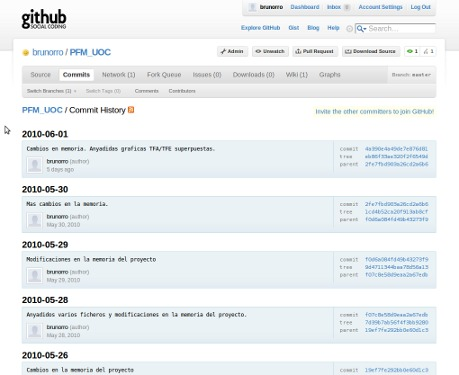
\includegraphics[width=11cm]{imagenes/interfazGit.jpg}
	\caption{Lista de commits de GitHub}
	\label{fig:interface_git}
\end{figure}

%%%%%%%%%%%%%%%%%%%%%%%%%%%%%%%%%%%%

\section{Planificación}
Se han estimado los siguientes puntos a los que imputar el tiempo empleado:
\begin{itemize}
	\item{\textbf{Diseño de la aplicación de gestión, captura y reconocimiento}: Tiempo durante el que se diseñarán los prototipos de las aplicaciones de las que consta el proyecto.}
	\item{\textbf{Diseño de la base de datos de gestión}: Tiempo empleado en diseñar la BD relacional que contendrá la información sobre el control de accesos.}
	\item{\textbf{Diseño de la base de datos de características}: Periodo durante el que se diseñará la BD relacional en la que se almacenará la representación facial de cada individuo.}
	\item{\textbf{Determinación de la representación en la BD}: Referente a la base de datos previa, durante este tiempo se investigará el método de almacenamiento para la representación facial.}
	\item{\textbf{Estadísticas}: Toma de datos y cálculos (gráficas) de eficiencia temporal, espacial y de funcionamiento.}
\end{itemize}
En la sección \ref{sec:cost_estimation} se definen los roles necesarios para llevar el proyecto, sus funciones y las estimaciones de tiempo de trabajo para cada uno de ellos. Tras la liberación se espera que los aspectos del desarrollo que no ha dado tiempo a finalizar (por falta de tiempo) se puedan pulir.

\chapter{Entorno del proyecto}

\section{Análisis de requerimientos}
%Condiciones de iluminación, fondo, fotografías, etc.
En la realización del proyecto se tomarán las siguientes consideraciones:
\begin{itemize}
	\item{Las condiciones de iluminación serán constantes o similares.}
	\item{Cuanto menos variaciones tenga el fondo sobre el que se capturará la imagen del sujeto en cuestión también será mejor la robustez del sistema}
	\item{Se debe de tener en cuenta que el sistema reconoce fotografías de individuos puestas frente a la cámara como tales. Habría que mantener algún tipo de control sobre este problema.}
\end{itemize}
	
Asimismo, también tenemos que tener en cuenta los problemas inherentes a todo sistema electrónico. La previsión de ellos incrementa el coste de implantación, a costa de mejorar la disponibilidad en todos los aspectos\cite{hiAvailability}:
\begin{itemize}
	\item{Fallos hardware (por desgaste). Para prevenir estos problemas, se debería replicar los componentes hardware que tengan posibilidad de fallo para dotar de alta disponibilidad a la infraestructura}
	\begin{itemize}
		\item{Duplicidad de fuentes de alimentación }
		\item{Replicación de discos duros: RAID1, RAID5, RAID10 o RAID01. }
		\item{Multiplicidad de accesos a red, lo cual no únicamente hace la infraestructura tolerante a fallos sino que puede agregar varias tarjetas de red (vía bonding o etherchannel/etherstack) }
		\item{En caso de almacenamiento compartido vía fibra óptica, replicación de HBA's\footnote{Host bus adapter, tarjetas que sirven para conectar las máquinas a la SAN.}. La replicación de switches de SAN también sería una alternativa a tener en cuenta, pero dispara el coste del sistema. }
	\end{itemize}

	\item{Cortes eléctricos}
	\begin{itemize}
		\item{Se hace necesaria la presencia de sistemas de alimentación ininterrumpida (SAIs) de capacidad calculada para la infraestructura.}
		\item{En caso de problemas más graves sería necesario tener un circuito alimentado por generadores o similares.}
	\end{itemize}

	\item{Infraestructura de comunicaciones: aquí los problemas no vienen dados sólo por el desgaste de los componentes, sino que además tenemos que tener en cuenta vulnerabilidades y ataques externos\footnote{A tener en cuenta el uso de rodenticidas. Los roedores tienen una afición especial por los cables UTP-5.}}
	\begin{itemize}
		\item{Contra los cortes en comunicaciones, se deberían tener replicadas las conexiones entre todos los switches utilizando STP (802.1W). Un ejemplo de redundancia se puede ver en la figura }
		\item{Uso de conexiones Gigabit o 10GbE }
		\item{Particionar la red de manera correcta en cuanto a VLAN's}
		\item{En caso de uso de redes inalámbricas, uso de encriptación WPA2 PSK o mejor. A ser posible, utilizar 802.1Q}
		\item{Tener bien separadas las máquinas de acceso externo en DMZs y utilizar VPN para accesos a la red interna. Comprobar la configuración de firewalls.}
	\end{itemize}

	\begin{figure}[h!]
        	\centering
		% Graphic for TeX using PGF
% Title: /home/bruno/pfc_UOC/PFM_UOC/memoria/diagramas/esquema_red.dia
% Creator: Dia v0.97
% CreationDate: Fri May 28 10:59:23 2010
% For: bruno
% \usepackage{tikz}
% The following commands are not supported in PSTricks at present
% We define them conditionally, so when they are implemented,
% this pgf file will use them.
\ifx\du\undefined
  \newlength{\du}
\fi
\setlength{\du}{15\unitlength}
\begin{tikzpicture}
\pgftransformxscale{1.000000}
\pgftransformyscale{-1.000000}
\definecolor{dialinecolor}{rgb}{0.000000, 0.000000, 0.000000}
\pgfsetstrokecolor{dialinecolor}
\definecolor{dialinecolor}{rgb}{1.000000, 1.000000, 1.000000}
\pgfsetfillcolor{dialinecolor}
\pgfsetlinewidth{0.100000\du}
\pgfsetdash{}{0pt}
\pgfsetdash{}{0pt}
\pgfsetroundjoin
{\pgfsetcornersarced{\pgfpoint{0.300000\du}{0.300000\du}}\definecolor{dialinecolor}{rgb}{0.960784, 0.980392, 0.764706}
\pgfsetfillcolor{dialinecolor}
\fill (1.000000\du,3.000000\du)--(1.000000\du,16.000000\du)--(15.000000\du,16.000000\du)--(15.000000\du,3.000000\du)--cycle;
}{\pgfsetcornersarced{\pgfpoint{0.300000\du}{0.300000\du}}\definecolor{dialinecolor}{rgb}{0.000000, 0.000000, 0.000000}
\pgfsetstrokecolor{dialinecolor}
\draw (1.000000\du,3.000000\du)--(1.000000\du,16.000000\du)--(15.000000\du,16.000000\du)--(15.000000\du,3.000000\du)--cycle;
}\pgfsetlinewidth{0.100000\du}
\pgfsetdash{}{0pt}
\pgfsetdash{}{0pt}
\pgfsetroundjoin
{\pgfsetcornersarced{\pgfpoint{0.300000\du}{0.300000\du}}\definecolor{dialinecolor}{rgb}{0.960784, 0.980392, 0.764706}
\pgfsetfillcolor{dialinecolor}
\fill (18.000000\du,3.000000\du)--(18.000000\du,16.000000\du)--(32.000000\du,16.000000\du)--(32.000000\du,3.000000\du)--cycle;
}{\pgfsetcornersarced{\pgfpoint{0.300000\du}{0.300000\du}}\definecolor{dialinecolor}{rgb}{0.000000, 0.000000, 0.000000}
\pgfsetstrokecolor{dialinecolor}
\draw (18.000000\du,3.000000\du)--(18.000000\du,16.000000\du)--(32.000000\du,16.000000\du)--(32.000000\du,3.000000\du)--cycle;
}\pgfsetlinewidth{0.100000\du}
\pgfsetdash{{\pgflinewidth}{0.200000\du}}{0cm}
\pgfsetdash{{\pgflinewidth}{0.200000\du}}{0cm}
\pgfsetbuttcap
\pgfsetmiterjoin
\pgfsetlinewidth{0.001000\du}
\pgfsetbuttcap
\pgfsetmiterjoin
\pgfsetdash{{\pgflinewidth}{0.200000\du}}{0cm}
\definecolor{dialinecolor}{rgb}{0.000000, 0.482353, 0.709804}
\pgfsetfillcolor{dialinecolor}
\pgfpathmoveto{\pgfpoint{9.374580\du}{5.588145\du}}
\pgfpathlineto{\pgfpoint{9.373052\du}{5.608921\du}}
\pgfpathlineto{\pgfpoint{9.368469\du}{5.629392\du}}
\pgfpathlineto{\pgfpoint{9.361137\du}{5.649557\du}}
\pgfpathlineto{\pgfpoint{9.350443\du}{5.669722\du}}
\pgfpathlineto{\pgfpoint{9.337000\du}{5.688970\du}}
\pgfpathlineto{\pgfpoint{9.321418\du}{5.708524\du}}
\pgfpathlineto{\pgfpoint{9.302475\du}{5.726856\du}}
\pgfpathlineto{\pgfpoint{9.281088\du}{5.745493\du}}
\pgfpathlineto{\pgfpoint{9.258173\du}{5.763520\du}}
\pgfpathlineto{\pgfpoint{9.231592\du}{5.780629\du}}
\pgfpathlineto{\pgfpoint{9.202872\du}{5.798045\du}}
\pgfpathlineto{\pgfpoint{9.172013\du}{5.814238\du}}
\pgfpathlineto{\pgfpoint{9.139627\du}{5.830431\du}}
\pgfpathlineto{\pgfpoint{9.103880\du}{5.845402\du}}
\pgfpathlineto{\pgfpoint{9.066911\du}{5.860373\du}}
\pgfpathlineto{\pgfpoint{9.027803\du}{5.874122\du}}
\pgfpathlineto{\pgfpoint{8.986557\du}{5.887565\du}}
\pgfpathlineto{\pgfpoint{8.943782\du}{5.900092\du}}
\pgfpathlineto{\pgfpoint{8.898870\du}{5.912313\du}}
\pgfpathlineto{\pgfpoint{8.853040\du}{5.923617\du}}
\pgfpathlineto{\pgfpoint{8.804155\du}{5.934005\du}}
\pgfpathlineto{\pgfpoint{8.754659\du}{5.943782\du}}
\pgfpathlineto{\pgfpoint{8.703941\du}{5.952948\du}}
\pgfpathlineto{\pgfpoint{8.651085\du}{5.961198\du}}
\pgfpathlineto{\pgfpoint{8.597617\du}{5.967919\du}}
\pgfpathlineto{\pgfpoint{8.542621\du}{5.974641\du}}
\pgfpathlineto{\pgfpoint{8.486709\du}{5.979835\du}}
\pgfpathlineto{\pgfpoint{8.429270\du}{5.984112\du}}
\pgfpathlineto{\pgfpoint{8.370608\du}{5.987779\du}}
\pgfpathlineto{\pgfpoint{8.311641\du}{5.990529\du}}
\pgfpathlineto{\pgfpoint{8.251757\du}{5.992362\du}}
\pgfpathlineto{\pgfpoint{8.190651\du}{5.992667\du}}
\pgfpathlineto{\pgfpoint{8.129850\du}{5.992362\du}}
\pgfpathlineto{\pgfpoint{8.069966\du}{5.990529\du}}
\pgfpathlineto{\pgfpoint{8.010999\du}{5.987779\du}}
\pgfpathlineto{\pgfpoint{7.952032\du}{5.984112\du}}
\pgfpathlineto{\pgfpoint{7.894898\du}{5.979835\du}}
\pgfpathlineto{\pgfpoint{7.838680\du}{5.974641\du}}
\pgfpathlineto{\pgfpoint{7.783685\du}{5.967919\du}}
\pgfpathlineto{\pgfpoint{7.730217\du}{5.961198\du}}
\pgfpathlineto{\pgfpoint{7.677971\du}{5.952948\du}}
\pgfpathlineto{\pgfpoint{7.626642\du}{5.943782\du}}
\pgfpathlineto{\pgfpoint{7.577452\du}{5.934005\du}}
\pgfpathlineto{\pgfpoint{7.528873\du}{5.923617\du}}
\pgfpathlineto{\pgfpoint{7.482432\du}{5.912313\du}}
\pgfpathlineto{\pgfpoint{7.437519\du}{5.900092\du}}
\pgfpathlineto{\pgfpoint{7.395050\du}{5.887565\du}}
\pgfpathlineto{\pgfpoint{7.353498\du}{5.874122\du}}
\pgfpathlineto{\pgfpoint{7.315002\du}{5.860373\du}}
\pgfpathlineto{\pgfpoint{7.277116\du}{5.845402\du}}
\pgfpathlineto{\pgfpoint{7.241980\du}{5.830431\du}}
\pgfpathlineto{\pgfpoint{7.209288\du}{5.814238\du}}
\pgfpathlineto{\pgfpoint{7.178430\du}{5.798045\du}}
\pgfpathlineto{\pgfpoint{7.149710\du}{5.780629\du}}
\pgfpathlineto{\pgfpoint{7.123434\du}{5.763520\du}}
\pgfpathlineto{\pgfpoint{7.100214\du}{5.745493\du}}
\pgfpathlineto{\pgfpoint{7.079132\du}{5.726856\du}}
\pgfpathlineto{\pgfpoint{7.059884\du}{5.708524\du}}
\pgfpathlineto{\pgfpoint{7.044302\du}{5.688970\du}}
\pgfpathlineto{\pgfpoint{7.030859\du}{5.669722\du}}
\pgfpathlineto{\pgfpoint{7.020471\du}{5.649557\du}}
\pgfpathlineto{\pgfpoint{7.013138\du}{5.629392\du}}
\pgfpathlineto{\pgfpoint{7.008555\du}{5.608921\du}}
\pgfpathlineto{\pgfpoint{7.007027\du}{5.588145\du}}
\pgfpathlineto{\pgfpoint{7.008555\du}{5.567064\du}}
\pgfpathlineto{\pgfpoint{7.013138\du}{5.546593\du}}
\pgfpathlineto{\pgfpoint{7.020471\du}{5.525817\du}}
\pgfpathlineto{\pgfpoint{7.030859\du}{5.506569\du}}
\pgfpathlineto{\pgfpoint{7.044302\du}{5.486709\du}}
\pgfpathlineto{\pgfpoint{7.059884\du}{5.467461\du}}
\pgfpathlineto{\pgfpoint{7.079132\du}{5.448518\du}}
\pgfpathlineto{\pgfpoint{7.100214\du}{5.430186\du}}
\pgfpathlineto{\pgfpoint{7.123434\du}{5.412466\du}}
\pgfpathlineto{\pgfpoint{7.149710\du}{5.395050\du}}
\pgfpathlineto{\pgfpoint{7.178430\du}{5.378246\du}}
\pgfpathlineto{\pgfpoint{7.209288\du}{5.361442\du}}
\pgfpathlineto{\pgfpoint{7.241980\du}{5.345860\du}}
\pgfpathlineto{\pgfpoint{7.277116\du}{5.330584\du}}
\pgfpathlineto{\pgfpoint{7.315002\du}{5.315613\du}}
\pgfpathlineto{\pgfpoint{7.353498\du}{5.301864\du}}
\pgfpathlineto{\pgfpoint{7.395050\du}{5.288420\du}}
\pgfpathlineto{\pgfpoint{7.437519\du}{5.275588\du}}
\pgfpathlineto{\pgfpoint{7.482432\du}{5.263367\du}}
\pgfpathlineto{\pgfpoint{7.528873\du}{5.252368\du}}
\pgfpathlineto{\pgfpoint{7.577452\du}{5.241674\du}}
\pgfpathlineto{\pgfpoint{7.626642\du}{5.231592\du}}
\pgfpathlineto{\pgfpoint{7.677971\du}{5.223342\du}}
\pgfpathlineto{\pgfpoint{7.730217\du}{5.215093\du}}
\pgfpathlineto{\pgfpoint{7.783685\du}{5.207760\du}}
\pgfpathlineto{\pgfpoint{7.838680\du}{5.201039\du}}
\pgfpathlineto{\pgfpoint{7.894898\du}{5.195845\du}}
\pgfpathlineto{\pgfpoint{7.952032\du}{5.191262\du}}
\pgfpathlineto{\pgfpoint{8.010999\du}{5.187595\du}}
\pgfpathlineto{\pgfpoint{8.069966\du}{5.185151\du}}
\pgfpathlineto{\pgfpoint{8.129850\du}{5.183318\du}}
\pgfpathlineto{\pgfpoint{8.190651\du}{5.183013\du}}
\pgfpathlineto{\pgfpoint{8.251757\du}{5.183318\du}}
\pgfpathlineto{\pgfpoint{8.311641\du}{5.185151\du}}
\pgfpathlineto{\pgfpoint{8.370608\du}{5.187595\du}}
\pgfpathlineto{\pgfpoint{8.429270\du}{5.191262\du}}
\pgfpathlineto{\pgfpoint{8.486709\du}{5.195845\du}}
\pgfpathlineto{\pgfpoint{8.542621\du}{5.201039\du}}
\pgfpathlineto{\pgfpoint{8.597617\du}{5.207760\du}}
\pgfpathlineto{\pgfpoint{8.651085\du}{5.215093\du}}
\pgfpathlineto{\pgfpoint{8.703941\du}{5.223342\du}}
\pgfpathlineto{\pgfpoint{8.754659\du}{5.231592\du}}
\pgfpathlineto{\pgfpoint{8.804155\du}{5.241674\du}}
\pgfpathlineto{\pgfpoint{8.853040\du}{5.252368\du}}
\pgfpathlineto{\pgfpoint{8.898870\du}{5.263367\du}}
\pgfpathlineto{\pgfpoint{8.943782\du}{5.275588\du}}
\pgfpathlineto{\pgfpoint{8.986557\du}{5.288420\du}}
\pgfpathlineto{\pgfpoint{9.027803\du}{5.301864\du}}
\pgfpathlineto{\pgfpoint{9.066911\du}{5.315613\du}}
\pgfpathlineto{\pgfpoint{9.103880\du}{5.330584\du}}
\pgfpathlineto{\pgfpoint{9.139627\du}{5.345860\du}}
\pgfpathlineto{\pgfpoint{9.172013\du}{5.361442\du}}
\pgfpathlineto{\pgfpoint{9.202872\du}{5.378246\du}}
\pgfpathlineto{\pgfpoint{9.231592\du}{5.395050\du}}
\pgfpathlineto{\pgfpoint{9.258173\du}{5.412466\du}}
\pgfpathlineto{\pgfpoint{9.281088\du}{5.430186\du}}
\pgfpathlineto{\pgfpoint{9.302475\du}{5.448518\du}}
\pgfpathlineto{\pgfpoint{9.321418\du}{5.467461\du}}
\pgfpathlineto{\pgfpoint{9.337000\du}{5.486709\du}}
\pgfpathlineto{\pgfpoint{9.350443\du}{5.506569\du}}
\pgfpathlineto{\pgfpoint{9.361137\du}{5.525817\du}}
\pgfpathlineto{\pgfpoint{9.368469\du}{5.546593\du}}
\pgfpathlineto{\pgfpoint{9.373052\du}{5.567064\du}}
\pgfpathlineto{\pgfpoint{9.374580\du}{5.588145\du}}
\pgfusepath{fill}
\pgfsetbuttcap
\pgfsetmiterjoin
\pgfsetdash{{\pgflinewidth}{0.200000\du}}{0cm}
\definecolor{dialinecolor}{rgb}{0.552941, 0.792157, 0.937255}
\pgfsetfillcolor{dialinecolor}
\pgfpathmoveto{\pgfpoint{8.190651\du}{6.000000\du}}
\pgfpathlineto{\pgfpoint{8.190651\du}{6.000000\du}}
\pgfpathlineto{\pgfpoint{8.221509\du}{6.000000\du}}
\pgfpathlineto{\pgfpoint{8.251757\du}{5.999389\du}}
\pgfpathlineto{\pgfpoint{8.282310\du}{5.998778\du}}
\pgfpathlineto{\pgfpoint{8.311641\du}{5.997861\du}}
\pgfpathlineto{\pgfpoint{8.341583\du}{5.996639\du}}
\pgfpathlineto{\pgfpoint{8.371525\du}{5.995112\du}}
\pgfpathlineto{\pgfpoint{8.400550\du}{5.993584\du}}
\pgfpathlineto{\pgfpoint{8.429881\du}{5.991751\du}}
\pgfpathlineto{\pgfpoint{8.458601\du}{5.989612\du}}
\pgfpathlineto{\pgfpoint{8.487321\du}{5.987168\du}}
\pgfpathlineto{\pgfpoint{8.515429\du}{5.984112\du}}
\pgfpathlineto{\pgfpoint{8.543538\du}{5.981668\du}}
\pgfpathlineto{\pgfpoint{8.570730\du}{5.978307\du}}
\pgfpathlineto{\pgfpoint{8.598228\du}{5.975558\du}}
\pgfpathlineto{\pgfpoint{8.625726\du}{5.971586\du}}
\pgfpathlineto{\pgfpoint{8.652612\du}{5.967919\du}}
\pgfpathlineto{\pgfpoint{8.678888\du}{5.963947\du}}
\pgfpathlineto{\pgfpoint{8.704858\du}{5.959976\du}}
\pgfpathlineto{\pgfpoint{8.731134\du}{5.955393\du}}
\pgfpathlineto{\pgfpoint{8.756187\du}{5.951115\du}}
\pgfpathlineto{\pgfpoint{8.781240\du}{5.945921\du}}
\pgfpathlineto{\pgfpoint{8.805988\du}{5.941338\du}}
\pgfpathlineto{\pgfpoint{8.830431\du}{5.936144\du}}
\pgfpathlineto{\pgfpoint{8.854568\du}{5.930645\du}}
\pgfpathlineto{\pgfpoint{8.877788\du}{5.924840\du}}
\pgfpathlineto{\pgfpoint{8.901008\du}{5.919035\du}}
\pgfpathlineto{\pgfpoint{8.923312\du}{5.913535\du}}
\pgfpathlineto{\pgfpoint{8.945310\du}{5.907424\du}}
\pgfpathlineto{\pgfpoint{8.956309\du}{5.903758\du}}
\pgfpathlineto{\pgfpoint{8.967308\du}{5.900703\du}}
\pgfpathlineto{\pgfpoint{8.978002\du}{5.897953\du}}
\pgfpathlineto{\pgfpoint{8.988695\du}{5.894287\du}}
\pgfpathlineto{\pgfpoint{8.999083\du}{5.891231\du}}
\pgfpathlineto{\pgfpoint{9.009471\du}{5.887565\du}}
\pgfpathlineto{\pgfpoint{9.019859\du}{5.884510\du}}
\pgfpathlineto{\pgfpoint{9.030247\du}{5.880843\du}}
\pgfpathlineto{\pgfpoint{9.040330\du}{5.877177\du}}
\pgfpathlineto{\pgfpoint{9.049801\du}{5.874122\du}}
\pgfpathlineto{\pgfpoint{9.059884\du}{5.870455\du}}
\pgfpathlineto{\pgfpoint{9.069050\du}{5.866789\du}}
\pgfpathlineto{\pgfpoint{9.079132\du}{5.863123\du}}
\pgfpathlineto{\pgfpoint{9.088298\du}{5.859762\du}}
\pgfpathlineto{\pgfpoint{9.097770\du}{5.855790\du}}
\pgfpathlineto{\pgfpoint{9.107241\du}{5.852123\du}}
\pgfpathlineto{\pgfpoint{9.116101\du}{5.848457\du}}
\pgfpathlineto{\pgfpoint{9.124656\du}{5.844791\du}}
\pgfpathlineto{\pgfpoint{9.133822\du}{5.840513\du}}
\pgfpathlineto{\pgfpoint{9.142071\du}{5.836847\du}}
\pgfpathlineto{\pgfpoint{9.151237\du}{5.832875\du}}
\pgfpathlineto{\pgfpoint{9.158876\du}{5.828598\du}}
\pgfpathlineto{\pgfpoint{9.167125\du}{5.824931\du}}
\pgfpathlineto{\pgfpoint{9.175680\du}{5.820348\du}}
\pgfpathlineto{\pgfpoint{9.183624\du}{5.816682\du}}
\pgfpathlineto{\pgfpoint{9.191262\du}{5.812099\du}}
\pgfpathlineto{\pgfpoint{9.199206\du}{5.808127\du}}
\pgfpathlineto{\pgfpoint{9.206538\du}{5.804155\du}}
\pgfpathlineto{\pgfpoint{9.214177\du}{5.799878\du}}
\pgfpathlineto{\pgfpoint{9.221509\du}{5.795600\du}}
\pgfpathlineto{\pgfpoint{9.228231\du}{5.791323\du}}
\pgfpathlineto{\pgfpoint{9.235258\du}{5.786740\du}}
\pgfpathlineto{\pgfpoint{9.242591\du}{5.782768\du}}
\pgfpathlineto{\pgfpoint{9.248701\du}{5.777880\du}}
\pgfpathlineto{\pgfpoint{9.255729\du}{5.773602\du}}
\pgfpathlineto{\pgfpoint{9.261839\du}{5.769325\du}}
\pgfpathlineto{\pgfpoint{9.267950\du}{5.764436\du}}
\pgfpathlineto{\pgfpoint{9.274672\du}{5.760159\du}}
\pgfpathlineto{\pgfpoint{9.279866\du}{5.755576\du}}
\pgfpathlineto{\pgfpoint{9.286587\du}{5.750993\du}}
\pgfpathlineto{\pgfpoint{9.291781\du}{5.746716\du}}
\pgfpathlineto{\pgfpoint{9.296670\du}{5.741522\du}}
\pgfpathlineto{\pgfpoint{9.302475\du}{5.737244\du}}
\pgfpathlineto{\pgfpoint{9.307669\du}{5.732050\du}}
\pgfpathlineto{\pgfpoint{9.312252\du}{5.727467\du}}
\pgfpathlineto{\pgfpoint{9.317446\du}{5.722884\du}}
\pgfpathlineto{\pgfpoint{9.321723\du}{5.717996\du}}
\pgfpathlineto{\pgfpoint{9.326917\du}{5.712802\du}}
\pgfpathlineto{\pgfpoint{9.330889\du}{5.708219\du}}
\pgfpathlineto{\pgfpoint{9.334861\du}{5.703330\du}}
\pgfpathlineto{\pgfpoint{9.339138\du}{5.698442\du}}
\pgfpathlineto{\pgfpoint{9.343416\du}{5.693248\du}}
\pgfpathlineto{\pgfpoint{9.346471\du}{5.688054\du}}
\pgfpathlineto{\pgfpoint{9.350137\du}{5.683471\du}}
\pgfpathlineto{\pgfpoint{9.353498\du}{5.678277\du}}
\pgfpathlineto{\pgfpoint{9.356859\du}{5.673388\du}}
\pgfpathlineto{\pgfpoint{9.359609\du}{5.667889\du}}
\pgfpathlineto{\pgfpoint{9.362664\du}{5.663000\du}}
\pgfpathlineto{\pgfpoint{9.365108\du}{5.657501\du}}
\pgfpathlineto{\pgfpoint{9.367247\du}{5.652307\du}}
\pgfpathlineto{\pgfpoint{9.369691\du}{5.647418\du}}
\pgfpathlineto{\pgfpoint{9.372136\du}{5.642224\du}}
\pgfpathlineto{\pgfpoint{9.373358\du}{5.636419\du}}
\pgfpathlineto{\pgfpoint{9.375191\du}{5.631531\du}}
\pgfpathlineto{\pgfpoint{9.376719\du}{5.626031\du}}
\pgfpathlineto{\pgfpoint{9.378246\du}{5.620837\du}}
\pgfpathlineto{\pgfpoint{9.379163\du}{5.615032\du}}
\pgfpathlineto{\pgfpoint{9.380385\du}{5.609838\du}}
\pgfpathlineto{\pgfpoint{9.380996\du}{5.604033\du}}
\pgfpathlineto{\pgfpoint{9.381607\du}{5.599145\du}}
\pgfpathlineto{\pgfpoint{9.381913\du}{5.593339\du}}
\pgfpathlineto{\pgfpoint{9.381913\du}{5.588145\du}}
\pgfpathlineto{\pgfpoint{9.367247\du}{5.588145\du}}
\pgfpathlineto{\pgfpoint{9.366942\du}{5.593034\du}}
\pgfpathlineto{\pgfpoint{9.366942\du}{5.597922\du}}
\pgfpathlineto{\pgfpoint{9.366942\du}{5.602811\du}}
\pgfpathlineto{\pgfpoint{9.365720\du}{5.607699\du}}
\pgfpathlineto{\pgfpoint{9.365108\du}{5.612588\du}}
\pgfpathlineto{\pgfpoint{9.364497\du}{5.617476\du}}
\pgfpathlineto{\pgfpoint{9.362970\du}{5.622365\du}}
\pgfpathlineto{\pgfpoint{9.361748\du}{5.626948\du}}
\pgfpathlineto{\pgfpoint{9.359914\du}{5.632447\du}}
\pgfpathlineto{\pgfpoint{9.358692\du}{5.636419\du}}
\pgfpathlineto{\pgfpoint{9.356248\du}{5.641613\du}}
\pgfpathlineto{\pgfpoint{9.354109\du}{5.646807\du}}
\pgfpathlineto{\pgfpoint{9.351665\du}{5.651696\du}}
\pgfpathlineto{\pgfpoint{9.349832\du}{5.655668\du}}
\pgfpathlineto{\pgfpoint{9.346777\du}{5.660862\du}}
\pgfpathlineto{\pgfpoint{9.344332\du}{5.666056\du}}
\pgfpathlineto{\pgfpoint{9.341888\du}{5.670333\du}}
\pgfpathlineto{\pgfpoint{9.338222\du}{5.675222\du}}
\pgfpathlineto{\pgfpoint{9.334861\du}{5.680416\du}}
\pgfpathlineto{\pgfpoint{9.331195\du}{5.684693\du}}
\pgfpathlineto{\pgfpoint{9.328139\du}{5.689276\du}}
\pgfpathlineto{\pgfpoint{9.323862\du}{5.693859\du}}
\pgfpathlineto{\pgfpoint{9.320501\du}{5.698747\du}}
\pgfpathlineto{\pgfpoint{9.316224\du}{5.703330\du}}
\pgfpathlineto{\pgfpoint{9.311641\du}{5.708219\du}}
\pgfpathlineto{\pgfpoint{9.307363\du}{5.712802\du}}
\pgfpathlineto{\pgfpoint{9.302475\du}{5.716774\du}}
\pgfpathlineto{\pgfpoint{9.297892\du}{5.721662\du}}
\pgfpathlineto{\pgfpoint{9.292698\du}{5.726245\du}}
\pgfpathlineto{\pgfpoint{9.288115\du}{5.730828\du}}
\pgfpathlineto{\pgfpoint{9.282615\du}{5.735716\du}}
\pgfpathlineto{\pgfpoint{9.277116\du}{5.739688\du}}
\pgfpathlineto{\pgfpoint{9.271311\du}{5.744271\du}}
\pgfpathlineto{\pgfpoint{9.265506\du}{5.748854\du}}
\pgfpathlineto{\pgfpoint{9.259701\du}{5.753132\du}}
\pgfpathlineto{\pgfpoint{9.253590\du}{5.757409\du}}
\pgfpathlineto{\pgfpoint{9.247174\du}{5.761992\du}}
\pgfpathlineto{\pgfpoint{9.241063\du}{5.766269\du}}
\pgfpathlineto{\pgfpoint{9.234647\du}{5.770241\du}}
\pgfpathlineto{\pgfpoint{9.227620\du}{5.774824\du}}
\pgfpathlineto{\pgfpoint{9.221204\du}{5.779102\du}}
\pgfpathlineto{\pgfpoint{9.214177\du}{5.783074\du}}
\pgfpathlineto{\pgfpoint{9.206538\du}{5.787351\du}}
\pgfpathlineto{\pgfpoint{9.199511\du}{5.791628\du}}
\pgfpathlineto{\pgfpoint{9.192484\du}{5.795600\du}}
\pgfpathlineto{\pgfpoint{9.184846\du}{5.799878\du}}
\pgfpathlineto{\pgfpoint{9.177207\du}{5.803544\du}}
\pgfpathlineto{\pgfpoint{9.168958\du}{5.807822\du}}
\pgfpathlineto{\pgfpoint{9.161014\du}{5.811793\du}}
\pgfpathlineto{\pgfpoint{9.153071\du}{5.815460\du}}
\pgfpathlineto{\pgfpoint{9.144821\du}{5.819737\du}}
\pgfpathlineto{\pgfpoint{9.135961\du}{5.823709\du}}
\pgfpathlineto{\pgfpoint{9.128017\du}{5.827375\du}}
\pgfpathlineto{\pgfpoint{9.118851\du}{5.831042\du}}
\pgfpathlineto{\pgfpoint{9.110602\du}{5.835014\du}}
\pgfpathlineto{\pgfpoint{9.101436\du}{5.838986\du}}
\pgfpathlineto{\pgfpoint{9.092270\du}{5.842652\du}}
\pgfpathlineto{\pgfpoint{9.083104\du}{5.846013\du}}
\pgfpathlineto{\pgfpoint{9.073633\du}{5.849985\du}}
\pgfpathlineto{\pgfpoint{9.064161\du}{5.853346\du}}
\pgfpathlineto{\pgfpoint{9.054995\du}{5.857012\du}}
\pgfpathlineto{\pgfpoint{9.044913\du}{5.860678\du}}
\pgfpathlineto{\pgfpoint{9.035136\du}{5.863734\du}}
\pgfpathlineto{\pgfpoint{9.025359\du}{5.867094\du}}
\pgfpathlineto{\pgfpoint{9.015277\du}{5.870761\du}}
\pgfpathlineto{\pgfpoint{9.005500\du}{5.874122\du}}
\pgfpathlineto{\pgfpoint{8.994806\du}{5.877177\du}}
\pgfpathlineto{\pgfpoint{8.984723\du}{5.880843\du}}
\pgfpathlineto{\pgfpoint{8.973724\du}{5.883899\du}}
\pgfpathlineto{\pgfpoint{8.963642\du}{5.887259\du}}
\pgfpathlineto{\pgfpoint{8.952643\du}{5.890009\du}}
\pgfpathlineto{\pgfpoint{8.941644\du}{5.893370\du}}
\pgfpathlineto{\pgfpoint{8.919646\du}{5.899481\du}}
\pgfpathlineto{\pgfpoint{8.897036\du}{5.905286\du}}
\pgfpathlineto{\pgfpoint{8.874427\du}{5.911091\du}}
\pgfpathlineto{\pgfpoint{8.851207\du}{5.916896\du}}
\pgfpathlineto{\pgfpoint{8.826764\du}{5.921784\du}}
\pgfpathlineto{\pgfpoint{8.803239\du}{5.926673\du}}
\pgfpathlineto{\pgfpoint{8.778796\du}{5.931867\du}}
\pgfpathlineto{\pgfpoint{8.753743\du}{5.936755\du}}
\pgfpathlineto{\pgfpoint{8.728689\du}{5.941338\du}}
\pgfpathlineto{\pgfpoint{8.702414\du}{5.945616\du}}
\pgfpathlineto{\pgfpoint{8.677055\du}{5.949588\du}}
\pgfpathlineto{\pgfpoint{8.650779\du}{5.953559\du}}
\pgfpathlineto{\pgfpoint{8.624198\du}{5.957226\du}}
\pgfpathlineto{\pgfpoint{8.597006\du}{5.961198\du}}
\pgfpathlineto{\pgfpoint{8.569203\du}{5.964253\du}}
\pgfpathlineto{\pgfpoint{8.542010\du}{5.967308\du}}
\pgfpathlineto{\pgfpoint{8.513902\du}{5.970058\du}}
\pgfpathlineto{\pgfpoint{8.485487\du}{5.972502\du}}
\pgfpathlineto{\pgfpoint{8.457684\du}{5.974947\du}}
\pgfpathlineto{\pgfpoint{8.428964\du}{5.977391\du}}
\pgfpathlineto{\pgfpoint{8.400244\du}{5.979529\du}}
\pgfpathlineto{\pgfpoint{8.370608\du}{5.981057\du}}
\pgfpathlineto{\pgfpoint{8.341583\du}{5.982279\du}}
\pgfpathlineto{\pgfpoint{8.311335\du}{5.983501\du}}
\pgfpathlineto{\pgfpoint{8.281699\du}{5.984112\du}}
\pgfpathlineto{\pgfpoint{8.251757\du}{5.985335\du}}
\pgfpathlineto{\pgfpoint{8.221204\du}{5.985335\du}}
\pgfpathlineto{\pgfpoint{8.190651\du}{5.985640\du}}
\pgfpathlineto{\pgfpoint{8.190651\du}{5.985640\du}}
\pgfpathlineto{\pgfpoint{8.190651\du}{5.985640\du}}
\pgfpathlineto{\pgfpoint{8.190040\du}{5.985640\du}}
\pgfpathlineto{\pgfpoint{8.189123\du}{5.985640\du}}
\pgfpathlineto{\pgfpoint{8.188512\du}{5.985640\du}}
\pgfpathlineto{\pgfpoint{8.187290\du}{5.985946\du}}
\pgfpathlineto{\pgfpoint{8.186984\du}{5.986557\du}}
\pgfpathlineto{\pgfpoint{8.186373\du}{5.986862\du}}
\pgfpathlineto{\pgfpoint{8.185762\du}{5.987168\du}}
\pgfpathlineto{\pgfpoint{8.185151\du}{5.987779\du}}
\pgfpathlineto{\pgfpoint{8.184846\du}{5.989001\du}}
\pgfpathlineto{\pgfpoint{8.184235\du}{5.990223\du}}
\pgfpathlineto{\pgfpoint{8.183624\du}{5.991445\du}}
\pgfpathlineto{\pgfpoint{8.183624\du}{5.992667\du}}
\pgfpathlineto{\pgfpoint{8.183624\du}{5.994195\du}}
\pgfpathlineto{\pgfpoint{8.184235\du}{5.995417\du}}
\pgfpathlineto{\pgfpoint{8.184846\du}{5.996639\du}}
\pgfpathlineto{\pgfpoint{8.185151\du}{5.997861\du}}
\pgfpathlineto{\pgfpoint{8.185762\du}{5.998472\du}}
\pgfpathlineto{\pgfpoint{8.186373\du}{5.998778\du}}
\pgfpathlineto{\pgfpoint{8.186984\du}{5.999083\du}}
\pgfpathlineto{\pgfpoint{8.187290\du}{5.999389\du}}
\pgfpathlineto{\pgfpoint{8.188512\du}{5.999389\du}}
\pgfpathlineto{\pgfpoint{8.189123\du}{6.000000\du}}
\pgfpathlineto{\pgfpoint{8.190040\du}{6.000000\du}}
\pgfpathlineto{\pgfpoint{8.190651\du}{6.000000\du}}
\pgfusepath{fill}
\pgfsetbuttcap
\pgfsetmiterjoin
\pgfsetdash{{\pgflinewidth}{0.200000\du}}{0cm}
\definecolor{dialinecolor}{rgb}{0.552941, 0.792157, 0.937255}
\pgfsetfillcolor{dialinecolor}
\pgfpathmoveto{\pgfpoint{7.000000\du}{5.588145\du}}
\pgfpathlineto{\pgfpoint{7.000000\du}{5.588145\du}}
\pgfpathlineto{\pgfpoint{7.000000\du}{5.593339\du}}
\pgfpathlineto{\pgfpoint{7.000000\du}{5.599145\du}}
\pgfpathlineto{\pgfpoint{7.000306\du}{5.604033\du}}
\pgfpathlineto{\pgfpoint{7.001222\du}{5.609838\du}}
\pgfpathlineto{\pgfpoint{7.002139\du}{5.615032\du}}
\pgfpathlineto{\pgfpoint{7.003666\du}{5.620837\du}}
\pgfpathlineto{\pgfpoint{7.004583\du}{5.626031\du}}
\pgfpathlineto{\pgfpoint{7.006111\du}{5.631531\du}}
\pgfpathlineto{\pgfpoint{7.007638\du}{5.636419\du}}
\pgfpathlineto{\pgfpoint{7.009471\du}{5.642224\du}}
\pgfpathlineto{\pgfpoint{7.011610\du}{5.647418\du}}
\pgfpathlineto{\pgfpoint{7.014054\du}{5.652307\du}}
\pgfpathlineto{\pgfpoint{7.016499\du}{5.657501\du}}
\pgfpathlineto{\pgfpoint{7.018943\du}{5.663000\du}}
\pgfpathlineto{\pgfpoint{7.021693\du}{5.667889\du}}
\pgfpathlineto{\pgfpoint{7.024748\du}{5.673388\du}}
\pgfpathlineto{\pgfpoint{7.027803\du}{5.678277\du}}
\pgfpathlineto{\pgfpoint{7.031470\du}{5.683471\du}}
\pgfpathlineto{\pgfpoint{7.035136\du}{5.688054\du}}
\pgfpathlineto{\pgfpoint{7.038191\du}{5.693248\du}}
\pgfpathlineto{\pgfpoint{7.042163\du}{5.698442\du}}
\pgfpathlineto{\pgfpoint{7.046746\du}{5.703330\du}}
\pgfpathlineto{\pgfpoint{7.050412\du}{5.708219\du}}
\pgfpathlineto{\pgfpoint{7.054384\du}{5.712802\du}}
\pgfpathlineto{\pgfpoint{7.059578\du}{5.717996\du}}
\pgfpathlineto{\pgfpoint{7.063856\du}{5.722884\du}}
\pgfpathlineto{\pgfpoint{7.068744\du}{5.727467\du}}
\pgfpathlineto{\pgfpoint{7.073938\du}{5.732050\du}}
\pgfpathlineto{\pgfpoint{7.079132\du}{5.737244\du}}
\pgfpathlineto{\pgfpoint{7.084326\du}{5.741522\du}}
\pgfpathlineto{\pgfpoint{7.089826\du}{5.746716\du}}
\pgfpathlineto{\pgfpoint{7.095325\du}{5.750993\du}}
\pgfpathlineto{\pgfpoint{7.101436\du}{5.755576\du}}
\pgfpathlineto{\pgfpoint{7.106936\du}{5.760159\du}}
\pgfpathlineto{\pgfpoint{7.113046\du}{5.764436\du}}
\pgfpathlineto{\pgfpoint{7.119462\du}{5.769325\du}}
\pgfpathlineto{\pgfpoint{7.125878\du}{5.773602\du}}
\pgfpathlineto{\pgfpoint{7.132600\du}{5.777880\du}}
\pgfpathlineto{\pgfpoint{7.139322\du}{5.782768\du}}
\pgfpathlineto{\pgfpoint{7.146043\du}{5.786740\du}}
\pgfpathlineto{\pgfpoint{7.153071\du}{5.791323\du}}
\pgfpathlineto{\pgfpoint{7.159792\du}{5.795600\du}}
\pgfpathlineto{\pgfpoint{7.167430\du}{5.799878\du}}
\pgfpathlineto{\pgfpoint{7.174763\du}{5.804155\du}}
\pgfpathlineto{\pgfpoint{7.182096\du}{5.808127\du}}
\pgfpathlineto{\pgfpoint{7.189734\du}{5.812099\du}}
\pgfpathlineto{\pgfpoint{7.197984\du}{5.816682\du}}
\pgfpathlineto{\pgfpoint{7.206233\du}{5.820348\du}}
\pgfpathlineto{\pgfpoint{7.214177\du}{5.824931\du}}
\pgfpathlineto{\pgfpoint{7.222426\du}{5.828598\du}}
\pgfpathlineto{\pgfpoint{7.230370\du}{5.832875\du}}
\pgfpathlineto{\pgfpoint{7.239536\du}{5.836847\du}}
\pgfpathlineto{\pgfpoint{7.248090\du}{5.840513\du}}
\pgfpathlineto{\pgfpoint{7.256645\du}{5.844791\du}}
\pgfpathlineto{\pgfpoint{7.265200\du}{5.848457\du}}
\pgfpathlineto{\pgfpoint{7.274366\du}{5.852123\du}}
\pgfpathlineto{\pgfpoint{7.283837\du}{5.855790\du}}
\pgfpathlineto{\pgfpoint{7.293003\du}{5.859762\du}}
\pgfpathlineto{\pgfpoint{7.302475\du}{5.863123\du}}
\pgfpathlineto{\pgfpoint{7.312252\du}{5.866789\du}}
\pgfpathlineto{\pgfpoint{7.321723\du}{5.870455\du}}
\pgfpathlineto{\pgfpoint{7.331500\du}{5.874122\du}}
\pgfpathlineto{\pgfpoint{7.341277\du}{5.877177\du}}
\pgfpathlineto{\pgfpoint{7.351360\du}{5.880843\du}}
\pgfpathlineto{\pgfpoint{7.361748\du}{5.884510\du}}
\pgfpathlineto{\pgfpoint{7.371830\du}{5.887565\du}}
\pgfpathlineto{\pgfpoint{7.382218\du}{5.891231\du}}
\pgfpathlineto{\pgfpoint{7.392606\du}{5.894287\du}}
\pgfpathlineto{\pgfpoint{7.403300\du}{5.897953\du}}
\pgfpathlineto{\pgfpoint{7.414299\du}{5.900703\du}}
\pgfpathlineto{\pgfpoint{7.424992\du}{5.903758\du}}
\pgfpathlineto{\pgfpoint{7.436297\du}{5.907424\du}}
\pgfpathlineto{\pgfpoint{7.458295\du}{5.913535\du}}
\pgfpathlineto{\pgfpoint{7.480599\du}{5.919035\du}}
\pgfpathlineto{\pgfpoint{7.503514\du}{5.924840\du}}
\pgfpathlineto{\pgfpoint{7.527039\du}{5.930645\du}}
\pgfpathlineto{\pgfpoint{7.551176\du}{5.936144\du}}
\pgfpathlineto{\pgfpoint{7.575619\du}{5.941338\du}}
\pgfpathlineto{\pgfpoint{7.600367\du}{5.945921\du}}
\pgfpathlineto{\pgfpoint{7.625420\du}{5.951115\du}}
\pgfpathlineto{\pgfpoint{7.650474\du}{5.955393\du}}
\pgfpathlineto{\pgfpoint{7.676749\du}{5.959976\du}}
\pgfpathlineto{\pgfpoint{7.702719\du}{5.963947\du}}
\pgfpathlineto{\pgfpoint{7.728689\du}{5.967919\du}}
\pgfpathlineto{\pgfpoint{7.756187\du}{5.971586\du}}
\pgfpathlineto{\pgfpoint{7.783074\du}{5.975558\du}}
\pgfpathlineto{\pgfpoint{7.810571\du}{5.978307\du}}
\pgfpathlineto{\pgfpoint{7.837764\du}{5.981668\du}}
\pgfpathlineto{\pgfpoint{7.865872\du}{5.984112\du}}
\pgfpathlineto{\pgfpoint{7.893981\du}{5.987168\du}}
\pgfpathlineto{\pgfpoint{7.922701\du}{5.989612\du}}
\pgfpathlineto{\pgfpoint{7.951726\du}{5.991751\du}}
\pgfpathlineto{\pgfpoint{7.980752\du}{5.993584\du}}
\pgfpathlineto{\pgfpoint{8.010082\du}{5.995112\du}}
\pgfpathlineto{\pgfpoint{8.039719\du}{5.996639\du}}
\pgfpathlineto{\pgfpoint{8.069966\du}{5.997861\du}}
\pgfpathlineto{\pgfpoint{8.099297\du}{5.998778\du}}
\pgfpathlineto{\pgfpoint{8.129545\du}{5.999389\du}}
\pgfpathlineto{\pgfpoint{8.160403\du}{6.000000\du}}
\pgfpathlineto{\pgfpoint{8.190651\du}{6.000000\du}}
\pgfpathlineto{\pgfpoint{8.190651\du}{5.985640\du}}
\pgfpathlineto{\pgfpoint{8.160403\du}{5.985335\du}}
\pgfpathlineto{\pgfpoint{8.129850\du}{5.985335\du}}
\pgfpathlineto{\pgfpoint{8.100214\du}{5.984112\du}}
\pgfpathlineto{\pgfpoint{8.070272\du}{5.983501\du}}
\pgfpathlineto{\pgfpoint{8.040024\du}{5.982279\du}}
\pgfpathlineto{\pgfpoint{8.010999\du}{5.981057\du}}
\pgfpathlineto{\pgfpoint{7.981363\du}{5.979529\du}}
\pgfpathlineto{\pgfpoint{7.952948\du}{5.977391\du}}
\pgfpathlineto{\pgfpoint{7.924229\du}{5.974947\du}}
\pgfpathlineto{\pgfpoint{7.895814\du}{5.972502\du}}
\pgfpathlineto{\pgfpoint{7.867705\du}{5.970058\du}}
\pgfpathlineto{\pgfpoint{7.839597\du}{5.967308\du}}
\pgfpathlineto{\pgfpoint{7.812405\du}{5.964253\du}}
\pgfpathlineto{\pgfpoint{7.784907\du}{5.961198\du}}
\pgfpathlineto{\pgfpoint{7.757409\du}{5.957226\du}}
\pgfpathlineto{\pgfpoint{7.730828\du}{5.953559\du}}
\pgfpathlineto{\pgfpoint{7.704552\du}{5.949588\du}}
\pgfpathlineto{\pgfpoint{7.678888\du}{5.945616\du}}
\pgfpathlineto{\pgfpoint{7.652918\du}{5.941338\du}}
\pgfpathlineto{\pgfpoint{7.628170\du}{5.936755\du}}
\pgfpathlineto{\pgfpoint{7.602811\du}{5.931867\du}}
\pgfpathlineto{\pgfpoint{7.578368\du}{5.926673\du}}
\pgfpathlineto{\pgfpoint{7.554537\du}{5.921784\du}}
\pgfpathlineto{\pgfpoint{7.530706\du}{5.916896\du}}
\pgfpathlineto{\pgfpoint{7.506874\du}{5.911091\du}}
\pgfpathlineto{\pgfpoint{7.484265\du}{5.905286\du}}
\pgfpathlineto{\pgfpoint{7.461962\du}{5.899481\du}}
\pgfpathlineto{\pgfpoint{7.439963\du}{5.893370\du}}
\pgfpathlineto{\pgfpoint{7.428964\du}{5.890009\du}}
\pgfpathlineto{\pgfpoint{7.417965\du}{5.887259\du}}
\pgfpathlineto{\pgfpoint{7.407577\du}{5.883899\du}}
\pgfpathlineto{\pgfpoint{7.397189\du}{5.880843\du}}
\pgfpathlineto{\pgfpoint{7.386496\du}{5.877177\du}}
\pgfpathlineto{\pgfpoint{7.376108\du}{5.874122\du}}
\pgfpathlineto{\pgfpoint{7.366636\du}{5.870761\du}}
\pgfpathlineto{\pgfpoint{7.355943\du}{5.867094\du}}
\pgfpathlineto{\pgfpoint{7.346471\du}{5.863734\du}}
\pgfpathlineto{\pgfpoint{7.336389\du}{5.860678\du}}
\pgfpathlineto{\pgfpoint{7.326306\du}{5.857012\du}}
\pgfpathlineto{\pgfpoint{7.317140\du}{5.853346\du}}
\pgfpathlineto{\pgfpoint{7.307669\du}{5.849985\du}}
\pgfpathlineto{\pgfpoint{7.298197\du}{5.846013\du}}
\pgfpathlineto{\pgfpoint{7.289031\du}{5.842652\du}}
\pgfpathlineto{\pgfpoint{7.280171\du}{5.838986\du}}
\pgfpathlineto{\pgfpoint{7.271005\du}{5.835014\du}}
\pgfpathlineto{\pgfpoint{7.262450\du}{5.831042\du}}
\pgfpathlineto{\pgfpoint{7.253896\du}{5.827375\du}}
\pgfpathlineto{\pgfpoint{7.245341\du}{5.823709\du}}
\pgfpathlineto{\pgfpoint{7.236786\du}{5.819737\du}}
\pgfpathlineto{\pgfpoint{7.228537\du}{5.815460\du}}
\pgfpathlineto{\pgfpoint{7.220287\du}{5.811793\du}}
\pgfpathlineto{\pgfpoint{7.212343\du}{5.807822\du}}
\pgfpathlineto{\pgfpoint{7.204094\du}{5.803544\du}}
\pgfpathlineto{\pgfpoint{7.196761\du}{5.799878\du}}
\pgfpathlineto{\pgfpoint{7.189123\du}{5.795600\du}}
\pgfpathlineto{\pgfpoint{7.181790\du}{5.791628\du}}
\pgfpathlineto{\pgfpoint{7.174763\du}{5.787351\du}}
\pgfpathlineto{\pgfpoint{7.167430\du}{5.783074\du}}
\pgfpathlineto{\pgfpoint{7.160403\du}{5.779102\du}}
\pgfpathlineto{\pgfpoint{7.153682\du}{5.774824\du}}
\pgfpathlineto{\pgfpoint{7.146960\du}{5.770241\du}}
\pgfpathlineto{\pgfpoint{7.140238\du}{5.765964\du}}
\pgfpathlineto{\pgfpoint{7.134433\du}{5.761992\du}}
\pgfpathlineto{\pgfpoint{7.128017\du}{5.757409\du}}
\pgfpathlineto{\pgfpoint{7.122212\du}{5.753132\du}}
\pgfpathlineto{\pgfpoint{7.115490\du}{5.748854\du}}
\pgfpathlineto{\pgfpoint{7.109991\du}{5.744271\du}}
\pgfpathlineto{\pgfpoint{7.104491\du}{5.739688\du}}
\pgfpathlineto{\pgfpoint{7.098686\du}{5.735716\du}}
\pgfpathlineto{\pgfpoint{7.093492\du}{5.730828\du}}
\pgfpathlineto{\pgfpoint{7.088604\du}{5.726245\du}}
\pgfpathlineto{\pgfpoint{7.084021\du}{5.721662\du}}
\pgfpathlineto{\pgfpoint{7.079132\du}{5.716774\du}}
\pgfpathlineto{\pgfpoint{7.074244\du}{5.712802\du}}
\pgfpathlineto{\pgfpoint{7.069661\du}{5.708219\du}}
\pgfpathlineto{\pgfpoint{7.065078\du}{5.703330\du}}
\pgfpathlineto{\pgfpoint{7.061106\du}{5.698747\du}}
\pgfpathlineto{\pgfpoint{7.057440\du}{5.693859\du}}
\pgfpathlineto{\pgfpoint{7.053468\du}{5.689276\du}}
\pgfpathlineto{\pgfpoint{7.050412\du}{5.684693\du}}
\pgfpathlineto{\pgfpoint{7.046746\du}{5.680416\du}}
\pgfpathlineto{\pgfpoint{7.043080\du}{5.675222\du}}
\pgfpathlineto{\pgfpoint{7.040024\du}{5.670333\du}}
\pgfpathlineto{\pgfpoint{7.036969\du}{5.666056\du}}
\pgfpathlineto{\pgfpoint{7.034525\du}{5.660862\du}}
\pgfpathlineto{\pgfpoint{7.031470\du}{5.655668\du}}
\pgfpathlineto{\pgfpoint{7.029025\du}{5.651696\du}}
\pgfpathlineto{\pgfpoint{7.027498\du}{5.646807\du}}
\pgfpathlineto{\pgfpoint{7.025053\du}{5.641613\du}}
\pgfpathlineto{\pgfpoint{7.022915\du}{5.636419\du}}
\pgfpathlineto{\pgfpoint{7.021387\du}{5.632447\du}}
\pgfpathlineto{\pgfpoint{7.019859\du}{5.626948\du}}
\pgfpathlineto{\pgfpoint{7.018332\du}{5.622365\du}}
\pgfpathlineto{\pgfpoint{7.017110\du}{5.617476\du}}
\pgfpathlineto{\pgfpoint{7.016499\du}{5.612588\du}}
\pgfpathlineto{\pgfpoint{7.015582\du}{5.607699\du}}
\pgfpathlineto{\pgfpoint{7.014665\du}{5.602811\du}}
\pgfpathlineto{\pgfpoint{7.014360\du}{5.597922\du}}
\pgfpathlineto{\pgfpoint{7.014360\du}{5.593034\du}}
\pgfpathlineto{\pgfpoint{7.014054\du}{5.588145\du}}
\pgfpathlineto{\pgfpoint{7.014054\du}{5.588145\du}}
\pgfpathlineto{\pgfpoint{7.014054\du}{5.588145\du}}
\pgfpathlineto{\pgfpoint{7.014054\du}{5.586923\du}}
\pgfpathlineto{\pgfpoint{7.014054\du}{5.586312\du}}
\pgfpathlineto{\pgfpoint{7.013443\du}{5.585701\du}}
\pgfpathlineto{\pgfpoint{7.013443\du}{5.584785\du}}
\pgfpathlineto{\pgfpoint{7.013138\du}{5.584479\du}}
\pgfpathlineto{\pgfpoint{7.012832\du}{5.583562\du}}
\pgfpathlineto{\pgfpoint{7.012221\du}{5.582951\du}}
\pgfpathlineto{\pgfpoint{7.012221\du}{5.582646\du}}
\pgfpathlineto{\pgfpoint{7.010694\du}{5.582035\du}}
\pgfpathlineto{\pgfpoint{7.009471\du}{5.581118\du}}
\pgfpathlineto{\pgfpoint{7.008555\du}{5.580507\du}}
\pgfpathlineto{\pgfpoint{7.007027\du}{5.580507\du}}
\pgfpathlineto{\pgfpoint{7.005194\du}{5.580507\du}}
\pgfpathlineto{\pgfpoint{7.003972\du}{5.581118\du}}
\pgfpathlineto{\pgfpoint{7.002750\du}{5.582035\du}}
\pgfpathlineto{\pgfpoint{7.001833\du}{5.582646\du}}
\pgfpathlineto{\pgfpoint{7.001222\du}{5.582951\du}}
\pgfpathlineto{\pgfpoint{7.000917\du}{5.583562\du}}
\pgfpathlineto{\pgfpoint{7.000306\du}{5.584479\du}}
\pgfpathlineto{\pgfpoint{7.000000\du}{5.584785\du}}
\pgfpathlineto{\pgfpoint{7.000000\du}{5.585701\du}}
\pgfpathlineto{\pgfpoint{7.000000\du}{5.586312\du}}
\pgfpathlineto{\pgfpoint{7.000000\du}{5.586923\du}}
\pgfpathlineto{\pgfpoint{7.000000\du}{5.588145\du}}
\pgfusepath{fill}
\pgfsetbuttcap
\pgfsetmiterjoin
\pgfsetdash{{\pgflinewidth}{0.200000\du}}{0cm}
\definecolor{dialinecolor}{rgb}{0.552941, 0.792157, 0.937255}
\pgfsetfillcolor{dialinecolor}
\pgfpathmoveto{\pgfpoint{8.190651\du}{5.175985\du}}
\pgfpathlineto{\pgfpoint{8.190651\du}{5.175985\du}}
\pgfpathlineto{\pgfpoint{8.160403\du}{5.175985\du}}
\pgfpathlineto{\pgfpoint{8.129545\du}{5.176291\du}}
\pgfpathlineto{\pgfpoint{8.099297\du}{5.176902\du}}
\pgfpathlineto{\pgfpoint{8.069966\du}{5.178124\du}}
\pgfpathlineto{\pgfpoint{8.039719\du}{5.179346\du}}
\pgfpathlineto{\pgfpoint{8.010082\du}{5.180568\du}}
\pgfpathlineto{\pgfpoint{7.980752\du}{5.182096\du}}
\pgfpathlineto{\pgfpoint{7.951726\du}{5.183929\du}}
\pgfpathlineto{\pgfpoint{7.922701\du}{5.186373\du}}
\pgfpathlineto{\pgfpoint{7.893981\du}{5.188818\du}}
\pgfpathlineto{\pgfpoint{7.865872\du}{5.191262\du}}
\pgfpathlineto{\pgfpoint{7.837764\du}{5.194012\du}}
\pgfpathlineto{\pgfpoint{7.810571\du}{5.197372\du}}
\pgfpathlineto{\pgfpoint{7.783074\du}{5.200733\du}}
\pgfpathlineto{\pgfpoint{7.756187\du}{5.204094\du}}
\pgfpathlineto{\pgfpoint{7.728689\du}{5.208066\du}}
\pgfpathlineto{\pgfpoint{7.702719\du}{5.211732\du}}
\pgfpathlineto{\pgfpoint{7.676749\du}{5.215704\du}}
\pgfpathlineto{\pgfpoint{7.650474\du}{5.220287\du}}
\pgfpathlineto{\pgfpoint{7.625420\du}{5.224870\du}}
\pgfpathlineto{\pgfpoint{7.600367\du}{5.229759\du}}
\pgfpathlineto{\pgfpoint{7.575619\du}{5.234647\du}}
\pgfpathlineto{\pgfpoint{7.551176\du}{5.240147\du}}
\pgfpathlineto{\pgfpoint{7.527039\du}{5.245035\du}}
\pgfpathlineto{\pgfpoint{7.503514\du}{5.250840\du}}
\pgfpathlineto{\pgfpoint{7.480599\du}{5.256340\du}}
\pgfpathlineto{\pgfpoint{7.458295\du}{5.262145\du}}
\pgfpathlineto{\pgfpoint{7.436297\du}{5.268561\du}}
\pgfpathlineto{\pgfpoint{7.414299\du}{5.274977\du}}
\pgfpathlineto{\pgfpoint{7.392606\du}{5.281393\du}}
\pgfpathlineto{\pgfpoint{7.382218\du}{5.284754\du}}
\pgfpathlineto{\pgfpoint{7.371830\du}{5.288115\du}}
\pgfpathlineto{\pgfpoint{7.361748\du}{5.291781\du}}
\pgfpathlineto{\pgfpoint{7.351360\du}{5.294837\du}}
\pgfpathlineto{\pgfpoint{7.341277\du}{5.298197\du}}
\pgfpathlineto{\pgfpoint{7.331500\du}{5.301864\du}}
\pgfpathlineto{\pgfpoint{7.321723\du}{5.305530\du}}
\pgfpathlineto{\pgfpoint{7.312252\du}{5.309196\du}}
\pgfpathlineto{\pgfpoint{7.302475\du}{5.312557\du}}
\pgfpathlineto{\pgfpoint{7.293003\du}{5.316224\du}}
\pgfpathlineto{\pgfpoint{7.283837\du}{5.319584\du}}
\pgfpathlineto{\pgfpoint{7.274366\du}{5.324167\du}}
\pgfpathlineto{\pgfpoint{7.265200\du}{5.327834\du}}
\pgfpathlineto{\pgfpoint{7.256645\du}{5.331500\du}}
\pgfpathlineto{\pgfpoint{7.248090\du}{5.335472\du}}
\pgfpathlineto{\pgfpoint{7.239536\du}{5.339138\du}}
\pgfpathlineto{\pgfpoint{7.230370\du}{5.343416\du}}
\pgfpathlineto{\pgfpoint{7.222426\du}{5.347388\du}}
\pgfpathlineto{\pgfpoint{7.214177\du}{5.351054\du}}
\pgfpathlineto{\pgfpoint{7.206233\du}{5.355332\du}}
\pgfpathlineto{\pgfpoint{7.197984\du}{5.359303\du}}
\pgfpathlineto{\pgfpoint{7.189734\du}{5.363275\du}}
\pgfpathlineto{\pgfpoint{7.182096\du}{5.367247\du}}
\pgfpathlineto{\pgfpoint{7.174763\du}{5.371525\du}}
\pgfpathlineto{\pgfpoint{7.167430\du}{5.376108\du}}
\pgfpathlineto{\pgfpoint{7.159792\du}{5.380079\du}}
\pgfpathlineto{\pgfpoint{7.153071\du}{5.384357\du}}
\pgfpathlineto{\pgfpoint{7.146043\du}{5.388940\du}}
\pgfpathlineto{\pgfpoint{7.139322\du}{5.393217\du}}
\pgfpathlineto{\pgfpoint{7.132600\du}{5.397800\du}}
\pgfpathlineto{\pgfpoint{7.125878\du}{5.402383\du}}
\pgfpathlineto{\pgfpoint{7.119462\du}{5.406355\du}}
\pgfpathlineto{\pgfpoint{7.113046\du}{5.410938\du}}
\pgfpathlineto{\pgfpoint{7.106936\du}{5.415826\du}}
\pgfpathlineto{\pgfpoint{7.101436\du}{5.420409\du}}
\pgfpathlineto{\pgfpoint{7.095325\du}{5.424992\du}}
\pgfpathlineto{\pgfpoint{7.089826\du}{5.429270\du}}
\pgfpathlineto{\pgfpoint{7.084326\du}{5.434158\du}}
\pgfpathlineto{\pgfpoint{7.079132\du}{5.438741\du}}
\pgfpathlineto{\pgfpoint{7.073938\du}{5.443630\du}}
\pgfpathlineto{\pgfpoint{7.068744\du}{5.448213\du}}
\pgfpathlineto{\pgfpoint{7.063856\du}{5.453101\du}}
\pgfpathlineto{\pgfpoint{7.059578\du}{5.457990\du}}
\pgfpathlineto{\pgfpoint{7.054384\du}{5.462573\du}}
\pgfpathlineto{\pgfpoint{7.050412\du}{5.467461\du}}
\pgfpathlineto{\pgfpoint{7.046746\du}{5.472350\du}}
\pgfpathlineto{\pgfpoint{7.042163\du}{5.477238\du}}
\pgfpathlineto{\pgfpoint{7.038191\du}{5.482738\du}}
\pgfpathlineto{\pgfpoint{7.035136\du}{5.487626\du}}
\pgfpathlineto{\pgfpoint{7.031470\du}{5.492515\du}}
\pgfpathlineto{\pgfpoint{7.027803\du}{5.497097\du}}
\pgfpathlineto{\pgfpoint{7.024748\du}{5.502903\du}}
\pgfpathlineto{\pgfpoint{7.021693\du}{5.507791\du}}
\pgfpathlineto{\pgfpoint{7.018943\du}{5.512985\du}}
\pgfpathlineto{\pgfpoint{7.016499\du}{5.517874\du}}
\pgfpathlineto{\pgfpoint{7.014054\du}{5.523373\du}}
\pgfpathlineto{\pgfpoint{7.011610\du}{5.528567\du}}
\pgfpathlineto{\pgfpoint{7.009471\du}{5.534067\du}}
\pgfpathlineto{\pgfpoint{7.007638\du}{5.539261\du}}
\pgfpathlineto{\pgfpoint{7.006111\du}{5.544455\du}}
\pgfpathlineto{\pgfpoint{7.004583\du}{5.549954\du}}
\pgfpathlineto{\pgfpoint{7.003666\du}{5.555148\du}}
\pgfpathlineto{\pgfpoint{7.002139\du}{5.560648\du}}
\pgfpathlineto{\pgfpoint{7.001222\du}{5.565842\du}}
\pgfpathlineto{\pgfpoint{7.000306\du}{5.571647\du}}
\pgfpathlineto{\pgfpoint{7.000000\du}{5.576841\du}}
\pgfpathlineto{\pgfpoint{7.000000\du}{5.582340\du}}
\pgfpathlineto{\pgfpoint{7.000000\du}{5.588145\du}}
\pgfpathlineto{\pgfpoint{7.014054\du}{5.588145\du}}
\pgfpathlineto{\pgfpoint{7.014360\du}{5.582951\du}}
\pgfpathlineto{\pgfpoint{7.014360\du}{5.577757\du}}
\pgfpathlineto{\pgfpoint{7.014665\du}{5.572869\du}}
\pgfpathlineto{\pgfpoint{7.015582\du}{5.567675\du}}
\pgfpathlineto{\pgfpoint{7.016499\du}{5.563092\du}}
\pgfpathlineto{\pgfpoint{7.017110\du}{5.558203\du}}
\pgfpathlineto{\pgfpoint{7.018332\du}{5.553621\du}}
\pgfpathlineto{\pgfpoint{7.019859\du}{5.548732\du}}
\pgfpathlineto{\pgfpoint{7.021387\du}{5.543844\du}}
\pgfpathlineto{\pgfpoint{7.022915\du}{5.538955\du}}
\pgfpathlineto{\pgfpoint{7.025053\du}{5.534067\du}}
\pgfpathlineto{\pgfpoint{7.027498\du}{5.529484\du}}
\pgfpathlineto{\pgfpoint{7.029025\du}{5.524595\du}}
\pgfpathlineto{\pgfpoint{7.031470\du}{5.519707\du}}
\pgfpathlineto{\pgfpoint{7.034525\du}{5.514207\du}}
\pgfpathlineto{\pgfpoint{7.036969\du}{5.510235\du}}
\pgfpathlineto{\pgfpoint{7.040024\du}{5.505347\du}}
\pgfpathlineto{\pgfpoint{7.043080\du}{5.500764\du}}
\pgfpathlineto{\pgfpoint{7.046746\du}{5.495875\du}}
\pgfpathlineto{\pgfpoint{7.050412\du}{5.491292\du}}
\pgfpathlineto{\pgfpoint{7.053468\du}{5.486404\du}}
\pgfpathlineto{\pgfpoint{7.057440\du}{5.481821\du}}
\pgfpathlineto{\pgfpoint{7.061106\du}{5.477238\du}}
\pgfpathlineto{\pgfpoint{7.065078\du}{5.472350\du}}
\pgfpathlineto{\pgfpoint{7.069661\du}{5.468072\du}}
\pgfpathlineto{\pgfpoint{7.074244\du}{5.462878\du}}
\pgfpathlineto{\pgfpoint{7.079132\du}{5.458906\du}}
\pgfpathlineto{\pgfpoint{7.084021\du}{5.454018\du}}
\pgfpathlineto{\pgfpoint{7.088604\du}{5.449435\du}}
\pgfpathlineto{\pgfpoint{7.093492\du}{5.444852\du}}
\pgfpathlineto{\pgfpoint{7.098686\du}{5.440574\du}}
\pgfpathlineto{\pgfpoint{7.104491\du}{5.435991\du}}
\pgfpathlineto{\pgfpoint{7.109991\du}{5.431408\du}}
\pgfpathlineto{\pgfpoint{7.115490\du}{5.427437\du}}
\pgfpathlineto{\pgfpoint{7.122212\du}{5.422548\du}}
\pgfpathlineto{\pgfpoint{7.128017\du}{5.418271\du}}
\pgfpathlineto{\pgfpoint{7.134433\du}{5.414299\du}}
\pgfpathlineto{\pgfpoint{7.140238\du}{5.409716\du}}
\pgfpathlineto{\pgfpoint{7.146960\du}{5.405438\du}}
\pgfpathlineto{\pgfpoint{7.153682\du}{5.401161\du}}
\pgfpathlineto{\pgfpoint{7.160403\du}{5.396884\du}}
\pgfpathlineto{\pgfpoint{7.167430\du}{5.392912\du}}
\pgfpathlineto{\pgfpoint{7.174763\du}{5.388940\du}}
\pgfpathlineto{\pgfpoint{7.181790\du}{5.384357\du}}
\pgfpathlineto{\pgfpoint{7.189123\du}{5.380079\du}}
\pgfpathlineto{\pgfpoint{7.196761\du}{5.376108\du}}
\pgfpathlineto{\pgfpoint{7.204094\du}{5.372136\du}}
\pgfpathlineto{\pgfpoint{7.212343\du}{5.367858\du}}
\pgfpathlineto{\pgfpoint{7.220287\du}{5.364192\du}}
\pgfpathlineto{\pgfpoint{7.228537\du}{5.360220\du}}
\pgfpathlineto{\pgfpoint{7.236786\du}{5.356554\du}}
\pgfpathlineto{\pgfpoint{7.245341\du}{5.351971\du}}
\pgfpathlineto{\pgfpoint{7.253896\du}{5.348610\du}}
\pgfpathlineto{\pgfpoint{7.262450\du}{5.344332\du}}
\pgfpathlineto{\pgfpoint{7.271005\du}{5.340972\du}}
\pgfpathlineto{\pgfpoint{7.280171\du}{5.337305\du}}
\pgfpathlineto{\pgfpoint{7.289031\du}{5.333333\du}}
\pgfpathlineto{\pgfpoint{7.298197\du}{5.329667\du}}
\pgfpathlineto{\pgfpoint{7.307669\du}{5.326001\du}}
\pgfpathlineto{\pgfpoint{7.317140\du}{5.322334\du}}
\pgfpathlineto{\pgfpoint{7.326306\du}{5.319279\du}}
\pgfpathlineto{\pgfpoint{7.336389\du}{5.315307\du}}
\pgfpathlineto{\pgfpoint{7.346471\du}{5.311641\du}}
\pgfpathlineto{\pgfpoint{7.355943\du}{5.308585\du}}
\pgfpathlineto{\pgfpoint{7.366636\du}{5.305225\du}}
\pgfpathlineto{\pgfpoint{7.376108\du}{5.301864\du}}
\pgfpathlineto{\pgfpoint{7.386496\du}{5.298503\du}}
\pgfpathlineto{\pgfpoint{7.397189\du}{5.295448\du}}
\pgfpathlineto{\pgfpoint{7.417965\du}{5.288726\du}}
\pgfpathlineto{\pgfpoint{7.439963\du}{5.282615\du}}
\pgfpathlineto{\pgfpoint{7.461962\du}{5.276505\du}}
\pgfpathlineto{\pgfpoint{7.484265\du}{5.270700\du}}
\pgfpathlineto{\pgfpoint{7.506874\du}{5.264895\du}}
\pgfpathlineto{\pgfpoint{7.530706\du}{5.259395\du}}
\pgfpathlineto{\pgfpoint{7.554537\du}{5.253896\du}}
\pgfpathlineto{\pgfpoint{7.578368\du}{5.248701\du}}
\pgfpathlineto{\pgfpoint{7.602811\du}{5.244119\du}}
\pgfpathlineto{\pgfpoint{7.628170\du}{5.239230\du}}
\pgfpathlineto{\pgfpoint{7.652918\du}{5.234647\du}}
\pgfpathlineto{\pgfpoint{7.678888\du}{5.229759\du}}
\pgfpathlineto{\pgfpoint{7.704552\du}{5.225787\du}}
\pgfpathlineto{\pgfpoint{7.730828\du}{5.222120\du}}
\pgfpathlineto{\pgfpoint{7.757409\du}{5.218148\du}}
\pgfpathlineto{\pgfpoint{7.784907\du}{5.215093\du}}
\pgfpathlineto{\pgfpoint{7.812405\du}{5.211732\du}}
\pgfpathlineto{\pgfpoint{7.839597\du}{5.208372\du}}
\pgfpathlineto{\pgfpoint{7.867705\du}{5.205622\du}}
\pgfpathlineto{\pgfpoint{7.895814\du}{5.202872\du}}
\pgfpathlineto{\pgfpoint{7.924229\du}{5.200733\du}}
\pgfpathlineto{\pgfpoint{7.952948\du}{5.198595\du}}
\pgfpathlineto{\pgfpoint{7.981363\du}{5.196456\du}}
\pgfpathlineto{\pgfpoint{8.010999\du}{5.194928\du}}
\pgfpathlineto{\pgfpoint{8.040024\du}{5.193401\du}}
\pgfpathlineto{\pgfpoint{8.070272\du}{5.192484\du}}
\pgfpathlineto{\pgfpoint{8.100214\du}{5.191567\du}}
\pgfpathlineto{\pgfpoint{8.129850\du}{5.190956\du}}
\pgfpathlineto{\pgfpoint{8.160403\du}{5.190345\du}}
\pgfpathlineto{\pgfpoint{8.190651\du}{5.190345\du}}
\pgfpathlineto{\pgfpoint{8.190651\du}{5.190345\du}}
\pgfpathlineto{\pgfpoint{8.190651\du}{5.190345\du}}
\pgfpathlineto{\pgfpoint{8.191873\du}{5.190345\du}}
\pgfpathlineto{\pgfpoint{8.192484\du}{5.189734\du}}
\pgfpathlineto{\pgfpoint{8.193095\du}{5.189734\du}}
\pgfpathlineto{\pgfpoint{8.194317\du}{5.189734\du}}
\pgfpathlineto{\pgfpoint{8.194317\du}{5.189734\du}}
\pgfpathlineto{\pgfpoint{8.195234\du}{5.189123\du}}
\pgfpathlineto{\pgfpoint{8.195845\du}{5.188512\du}}
\pgfpathlineto{\pgfpoint{8.196150\du}{5.187595\du}}
\pgfpathlineto{\pgfpoint{8.196761\du}{5.186984\du}}
\pgfpathlineto{\pgfpoint{8.197984\du}{5.185762\du}}
\pgfpathlineto{\pgfpoint{8.197984\du}{5.184540\du}}
\pgfpathlineto{\pgfpoint{8.198289\du}{5.183013\du}}
\pgfpathlineto{\pgfpoint{8.197984\du}{5.181790\du}}
\pgfpathlineto{\pgfpoint{8.197984\du}{5.180568\du}}
\pgfpathlineto{\pgfpoint{8.196761\du}{5.179346\du}}
\pgfpathlineto{\pgfpoint{8.196150\du}{5.178124\du}}
\pgfpathlineto{\pgfpoint{8.195845\du}{5.177819\du}}
\pgfpathlineto{\pgfpoint{8.195234\du}{5.177207\du}}
\pgfpathlineto{\pgfpoint{8.194317\du}{5.176902\du}}
\pgfpathlineto{\pgfpoint{8.194317\du}{5.176291\du}}
\pgfpathlineto{\pgfpoint{8.193095\du}{5.176291\du}}
\pgfpathlineto{\pgfpoint{8.192484\du}{5.175985\du}}
\pgfpathlineto{\pgfpoint{8.191873\du}{5.175985\du}}
\pgfpathlineto{\pgfpoint{8.190651\du}{5.175985\du}}
\pgfusepath{fill}
\pgfsetbuttcap
\pgfsetmiterjoin
\pgfsetdash{{\pgflinewidth}{0.200000\du}}{0cm}
\definecolor{dialinecolor}{rgb}{0.552941, 0.792157, 0.937255}
\pgfsetfillcolor{dialinecolor}
\pgfpathmoveto{\pgfpoint{9.381913\du}{5.588145\du}}
\pgfpathlineto{\pgfpoint{9.381913\du}{5.582340\du}}
\pgfpathlineto{\pgfpoint{9.381607\du}{5.576841\du}}
\pgfpathlineto{\pgfpoint{9.380996\du}{5.571647\du}}
\pgfpathlineto{\pgfpoint{9.380385\du}{5.565842\du}}
\pgfpathlineto{\pgfpoint{9.379163\du}{5.560648\du}}
\pgfpathlineto{\pgfpoint{9.378246\du}{5.555148\du}}
\pgfpathlineto{\pgfpoint{9.376719\du}{5.549954\du}}
\pgfpathlineto{\pgfpoint{9.375191\du}{5.544455\du}}
\pgfpathlineto{\pgfpoint{9.373358\du}{5.539261\du}}
\pgfpathlineto{\pgfpoint{9.372136\du}{5.534067\du}}
\pgfpathlineto{\pgfpoint{9.369691\du}{5.528567\du}}
\pgfpathlineto{\pgfpoint{9.367247\du}{5.523373\du}}
\pgfpathlineto{\pgfpoint{9.365108\du}{5.517874\du}}
\pgfpathlineto{\pgfpoint{9.362664\du}{5.512985\du}}
\pgfpathlineto{\pgfpoint{9.359609\du}{5.507791\du}}
\pgfpathlineto{\pgfpoint{9.356859\du}{5.502903\du}}
\pgfpathlineto{\pgfpoint{9.353498\du}{5.497097\du}}
\pgfpathlineto{\pgfpoint{9.350137\du}{5.492515\du}}
\pgfpathlineto{\pgfpoint{9.346471\du}{5.487626\du}}
\pgfpathlineto{\pgfpoint{9.343416\du}{5.482738\du}}
\pgfpathlineto{\pgfpoint{9.339138\du}{5.477238\du}}
\pgfpathlineto{\pgfpoint{9.334861\du}{5.472350\du}}
\pgfpathlineto{\pgfpoint{9.330889\du}{5.467461\du}}
\pgfpathlineto{\pgfpoint{9.326917\du}{5.462573\du}}
\pgfpathlineto{\pgfpoint{9.321723\du}{5.457990\du}}
\pgfpathlineto{\pgfpoint{9.317446\du}{5.453101\du}}
\pgfpathlineto{\pgfpoint{9.312252\du}{5.448213\du}}
\pgfpathlineto{\pgfpoint{9.307669\du}{5.443630\du}}
\pgfpathlineto{\pgfpoint{9.302475\du}{5.438741\du}}
\pgfpathlineto{\pgfpoint{9.296670\du}{5.434158\du}}
\pgfpathlineto{\pgfpoint{9.291781\du}{5.429270\du}}
\pgfpathlineto{\pgfpoint{9.286587\du}{5.424992\du}}
\pgfpathlineto{\pgfpoint{9.279866\du}{5.420409\du}}
\pgfpathlineto{\pgfpoint{9.274672\du}{5.415826\du}}
\pgfpathlineto{\pgfpoint{9.267950\du}{5.410938\du}}
\pgfpathlineto{\pgfpoint{9.261839\du}{5.406355\du}}
\pgfpathlineto{\pgfpoint{9.255729\du}{5.402383\du}}
\pgfpathlineto{\pgfpoint{9.248701\du}{5.397800\du}}
\pgfpathlineto{\pgfpoint{9.242591\du}{5.393217\du}}
\pgfpathlineto{\pgfpoint{9.235258\du}{5.388940\du}}
\pgfpathlineto{\pgfpoint{9.228231\du}{5.384357\du}}
\pgfpathlineto{\pgfpoint{9.221509\du}{5.380079\du}}
\pgfpathlineto{\pgfpoint{9.214177\du}{5.376108\du}}
\pgfpathlineto{\pgfpoint{9.206538\du}{5.371525\du}}
\pgfpathlineto{\pgfpoint{9.199206\du}{5.367247\du}}
\pgfpathlineto{\pgfpoint{9.191262\du}{5.363275\du}}
\pgfpathlineto{\pgfpoint{9.183624\du}{5.359303\du}}
\pgfpathlineto{\pgfpoint{9.175680\du}{5.355332\du}}
\pgfpathlineto{\pgfpoint{9.167125\du}{5.351054\du}}
\pgfpathlineto{\pgfpoint{9.158876\du}{5.347388\du}}
\pgfpathlineto{\pgfpoint{9.151237\du}{5.343416\du}}
\pgfpathlineto{\pgfpoint{9.142071\du}{5.339138\du}}
\pgfpathlineto{\pgfpoint{9.133822\du}{5.335472\du}}
\pgfpathlineto{\pgfpoint{9.124656\du}{5.331500\du}}
\pgfpathlineto{\pgfpoint{9.116101\du}{5.327834\du}}
\pgfpathlineto{\pgfpoint{9.107241\du}{5.324167\du}}
\pgfpathlineto{\pgfpoint{9.097770\du}{5.319584\du}}
\pgfpathlineto{\pgfpoint{9.088298\du}{5.316224\du}}
\pgfpathlineto{\pgfpoint{9.079132\du}{5.312557\du}}
\pgfpathlineto{\pgfpoint{9.069050\du}{5.309196\du}}
\pgfpathlineto{\pgfpoint{9.059884\du}{5.305530\du}}
\pgfpathlineto{\pgfpoint{9.049801\du}{5.301864\du}}
\pgfpathlineto{\pgfpoint{9.040330\du}{5.298197\du}}
\pgfpathlineto{\pgfpoint{9.030247\du}{5.294837\du}}
\pgfpathlineto{\pgfpoint{9.019859\du}{5.291781\du}}
\pgfpathlineto{\pgfpoint{9.009471\du}{5.288115\du}}
\pgfpathlineto{\pgfpoint{8.999083\du}{5.284754\du}}
\pgfpathlineto{\pgfpoint{8.988695\du}{5.281393\du}}
\pgfpathlineto{\pgfpoint{8.967308\du}{5.274977\du}}
\pgfpathlineto{\pgfpoint{8.945310\du}{5.268561\du}}
\pgfpathlineto{\pgfpoint{8.923312\du}{5.262145\du}}
\pgfpathlineto{\pgfpoint{8.901008\du}{5.256340\du}}
\pgfpathlineto{\pgfpoint{8.877788\du}{5.250840\du}}
\pgfpathlineto{\pgfpoint{8.854568\du}{5.245035\du}}
\pgfpathlineto{\pgfpoint{8.830431\du}{5.240147\du}}
\pgfpathlineto{\pgfpoint{8.805988\du}{5.234647\du}}
\pgfpathlineto{\pgfpoint{8.781240\du}{5.229759\du}}
\pgfpathlineto{\pgfpoint{8.756187\du}{5.224870\du}}
\pgfpathlineto{\pgfpoint{8.731134\du}{5.220287\du}}
\pgfpathlineto{\pgfpoint{8.704858\du}{5.215704\du}}
\pgfpathlineto{\pgfpoint{8.678888\du}{5.211732\du}}
\pgfpathlineto{\pgfpoint{8.652612\du}{5.208066\du}}
\pgfpathlineto{\pgfpoint{8.625726\du}{5.204094\du}}
\pgfpathlineto{\pgfpoint{8.598228\du}{5.200733\du}}
\pgfpathlineto{\pgfpoint{8.570730\du}{5.197372\du}}
\pgfpathlineto{\pgfpoint{8.543538\du}{5.194012\du}}
\pgfpathlineto{\pgfpoint{8.515429\du}{5.191262\du}}
\pgfpathlineto{\pgfpoint{8.487321\du}{5.188818\du}}
\pgfpathlineto{\pgfpoint{8.458601\du}{5.186373\du}}
\pgfpathlineto{\pgfpoint{8.429881\du}{5.183929\du}}
\pgfpathlineto{\pgfpoint{8.400550\du}{5.182096\du}}
\pgfpathlineto{\pgfpoint{8.371525\du}{5.180568\du}}
\pgfpathlineto{\pgfpoint{8.341583\du}{5.179346\du}}
\pgfpathlineto{\pgfpoint{8.311641\du}{5.178124\du}}
\pgfpathlineto{\pgfpoint{8.282310\du}{5.176902\du}}
\pgfpathlineto{\pgfpoint{8.251757\du}{5.176291\du}}
\pgfpathlineto{\pgfpoint{8.221509\du}{5.175985\du}}
\pgfpathlineto{\pgfpoint{8.190651\du}{5.175985\du}}
\pgfpathlineto{\pgfpoint{8.190651\du}{5.190345\du}}
\pgfpathlineto{\pgfpoint{8.221204\du}{5.190345\du}}
\pgfpathlineto{\pgfpoint{8.251757\du}{5.190956\du}}
\pgfpathlineto{\pgfpoint{8.281699\du}{5.191567\du}}
\pgfpathlineto{\pgfpoint{8.311335\du}{5.192484\du}}
\pgfpathlineto{\pgfpoint{8.341583\du}{5.193401\du}}
\pgfpathlineto{\pgfpoint{8.370608\du}{5.194928\du}}
\pgfpathlineto{\pgfpoint{8.400244\du}{5.196456\du}}
\pgfpathlineto{\pgfpoint{8.428964\du}{5.198595\du}}
\pgfpathlineto{\pgfpoint{8.457684\du}{5.200733\du}}
\pgfpathlineto{\pgfpoint{8.485487\du}{5.202872\du}}
\pgfpathlineto{\pgfpoint{8.513902\du}{5.205622\du}}
\pgfpathlineto{\pgfpoint{8.542010\du}{5.208372\du}}
\pgfpathlineto{\pgfpoint{8.569203\du}{5.211732\du}}
\pgfpathlineto{\pgfpoint{8.597006\du}{5.215093\du}}
\pgfpathlineto{\pgfpoint{8.624198\du}{5.218148\du}}
\pgfpathlineto{\pgfpoint{8.650779\du}{5.222120\du}}
\pgfpathlineto{\pgfpoint{8.677055\du}{5.225787\du}}
\pgfpathlineto{\pgfpoint{8.702414\du}{5.229759\du}}
\pgfpathlineto{\pgfpoint{8.728689\du}{5.234647\du}}
\pgfpathlineto{\pgfpoint{8.753743\du}{5.239230\du}}
\pgfpathlineto{\pgfpoint{8.778796\du}{5.244119\du}}
\pgfpathlineto{\pgfpoint{8.803239\du}{5.248701\du}}
\pgfpathlineto{\pgfpoint{8.826764\du}{5.253896\du}}
\pgfpathlineto{\pgfpoint{8.851207\du}{5.259395\du}}
\pgfpathlineto{\pgfpoint{8.874427\du}{5.264895\du}}
\pgfpathlineto{\pgfpoint{8.897036\du}{5.270700\du}}
\pgfpathlineto{\pgfpoint{8.919646\du}{5.276505\du}}
\pgfpathlineto{\pgfpoint{8.941644\du}{5.282615\du}}
\pgfpathlineto{\pgfpoint{8.963642\du}{5.288726\du}}
\pgfpathlineto{\pgfpoint{8.984723\du}{5.295448\du}}
\pgfpathlineto{\pgfpoint{8.994806\du}{5.298503\du}}
\pgfpathlineto{\pgfpoint{9.005500\du}{5.301864\du}}
\pgfpathlineto{\pgfpoint{9.015277\du}{5.305225\du}}
\pgfpathlineto{\pgfpoint{9.025359\du}{5.308585\du}}
\pgfpathlineto{\pgfpoint{9.035136\du}{5.311641\du}}
\pgfpathlineto{\pgfpoint{9.044913\du}{5.315307\du}}
\pgfpathlineto{\pgfpoint{9.054995\du}{5.319279\du}}
\pgfpathlineto{\pgfpoint{9.064161\du}{5.322334\du}}
\pgfpathlineto{\pgfpoint{9.073633\du}{5.326001\du}}
\pgfpathlineto{\pgfpoint{9.083104\du}{5.329667\du}}
\pgfpathlineto{\pgfpoint{9.092270\du}{5.333333\du}}
\pgfpathlineto{\pgfpoint{9.101436\du}{5.337305\du}}
\pgfpathlineto{\pgfpoint{9.110602\du}{5.340972\du}}
\pgfpathlineto{\pgfpoint{9.118851\du}{5.344332\du}}
\pgfpathlineto{\pgfpoint{9.128017\du}{5.348610\du}}
\pgfpathlineto{\pgfpoint{9.135961\du}{5.351971\du}}
\pgfpathlineto{\pgfpoint{9.144821\du}{5.356554\du}}
\pgfpathlineto{\pgfpoint{9.153071\du}{5.360220\du}}
\pgfpathlineto{\pgfpoint{9.161014\du}{5.364192\du}}
\pgfpathlineto{\pgfpoint{9.168958\du}{5.367858\du}}
\pgfpathlineto{\pgfpoint{9.177207\du}{5.372136\du}}
\pgfpathlineto{\pgfpoint{9.184846\du}{5.376108\du}}
\pgfpathlineto{\pgfpoint{9.192484\du}{5.380079\du}}
\pgfpathlineto{\pgfpoint{9.199511\du}{5.384357\du}}
\pgfpathlineto{\pgfpoint{9.206538\du}{5.388940\du}}
\pgfpathlineto{\pgfpoint{9.214177\du}{5.392912\du}}
\pgfpathlineto{\pgfpoint{9.221204\du}{5.396884\du}}
\pgfpathlineto{\pgfpoint{9.227620\du}{5.401161\du}}
\pgfpathlineto{\pgfpoint{9.234647\du}{5.405438\du}}
\pgfpathlineto{\pgfpoint{9.241063\du}{5.409716\du}}
\pgfpathlineto{\pgfpoint{9.247174\du}{5.414299\du}}
\pgfpathlineto{\pgfpoint{9.253590\du}{5.418271\du}}
\pgfpathlineto{\pgfpoint{9.259701\du}{5.422548\du}}
\pgfpathlineto{\pgfpoint{9.265506\du}{5.427437\du}}
\pgfpathlineto{\pgfpoint{9.271311\du}{5.431408\du}}
\pgfpathlineto{\pgfpoint{9.277116\du}{5.435991\du}}
\pgfpathlineto{\pgfpoint{9.282615\du}{5.440574\du}}
\pgfpathlineto{\pgfpoint{9.288115\du}{5.444852\du}}
\pgfpathlineto{\pgfpoint{9.292698\du}{5.449435\du}}
\pgfpathlineto{\pgfpoint{9.297892\du}{5.454018\du}}
\pgfpathlineto{\pgfpoint{9.302475\du}{5.458906\du}}
\pgfpathlineto{\pgfpoint{9.307363\du}{5.462878\du}}
\pgfpathlineto{\pgfpoint{9.311641\du}{5.468072\du}}
\pgfpathlineto{\pgfpoint{9.316224\du}{5.472350\du}}
\pgfpathlineto{\pgfpoint{9.320501\du}{5.477238\du}}
\pgfpathlineto{\pgfpoint{9.323862\du}{5.481821\du}}
\pgfpathlineto{\pgfpoint{9.328139\du}{5.486404\du}}
\pgfpathlineto{\pgfpoint{9.331195\du}{5.491292\du}}
\pgfpathlineto{\pgfpoint{9.334861\du}{5.495875\du}}
\pgfpathlineto{\pgfpoint{9.338222\du}{5.500764\du}}
\pgfpathlineto{\pgfpoint{9.341888\du}{5.505347\du}}
\pgfpathlineto{\pgfpoint{9.344332\du}{5.510235\du}}
\pgfpathlineto{\pgfpoint{9.346777\du}{5.514207\du}}
\pgfpathlineto{\pgfpoint{9.349832\du}{5.519707\du}}
\pgfpathlineto{\pgfpoint{9.351665\du}{5.524595\du}}
\pgfpathlineto{\pgfpoint{9.354109\du}{5.529484\du}}
\pgfpathlineto{\pgfpoint{9.356248\du}{5.534067\du}}
\pgfpathlineto{\pgfpoint{9.358692\du}{5.538955\du}}
\pgfpathlineto{\pgfpoint{9.359914\du}{5.543844\du}}
\pgfpathlineto{\pgfpoint{9.361748\du}{5.548732\du}}
\pgfpathlineto{\pgfpoint{9.362970\du}{5.553621\du}}
\pgfpathlineto{\pgfpoint{9.364497\du}{5.558203\du}}
\pgfpathlineto{\pgfpoint{9.365108\du}{5.563092\du}}
\pgfpathlineto{\pgfpoint{9.365720\du}{5.567675\du}}
\pgfpathlineto{\pgfpoint{9.366942\du}{5.572869\du}}
\pgfpathlineto{\pgfpoint{9.366942\du}{5.577757\du}}
\pgfpathlineto{\pgfpoint{9.366942\du}{5.582951\du}}
\pgfpathlineto{\pgfpoint{9.367247\du}{5.588145\du}}
\pgfpathlineto{\pgfpoint{9.381913\du}{5.588145\du}}
\pgfusepath{fill}
\pgfsetbuttcap
\pgfsetmiterjoin
\pgfsetdash{{\pgflinewidth}{0.200000\du}}{0cm}
\definecolor{dialinecolor}{rgb}{0.000000, 0.482353, 0.709804}
\pgfsetfillcolor{dialinecolor}
\pgfpathmoveto{\pgfpoint{7.003666\du}{4.760464\du}}
\pgfpathlineto{\pgfpoint{7.003666\du}{5.598839\du}}
\pgfpathlineto{\pgfpoint{9.374580\du}{5.598839\du}}
\pgfpathlineto{\pgfpoint{9.374580\du}{4.760770\du}}
\pgfpathlineto{\pgfpoint{7.003666\du}{4.760464\du}}
\pgfusepath{fill}
\pgfsetbuttcap
\pgfsetmiterjoin
\pgfsetdash{{\pgflinewidth}{0.200000\du}}{0cm}
\definecolor{dialinecolor}{rgb}{0.000000, 0.607843, 0.874510}
\pgfsetfillcolor{dialinecolor}
\pgfpathmoveto{\pgfpoint{9.374580\du}{4.735105\du}}
\pgfpathlineto{\pgfpoint{9.373052\du}{4.755881\du}}
\pgfpathlineto{\pgfpoint{9.368469\du}{4.776352\du}}
\pgfpathlineto{\pgfpoint{9.361137\du}{4.796211\du}}
\pgfpathlineto{\pgfpoint{9.350443\du}{4.816682\du}}
\pgfpathlineto{\pgfpoint{9.337000\du}{4.835930\du}}
\pgfpathlineto{\pgfpoint{9.321418\du}{4.855179\du}}
\pgfpathlineto{\pgfpoint{9.302475\du}{4.873816\du}}
\pgfpathlineto{\pgfpoint{9.281088\du}{4.892453\du}}
\pgfpathlineto{\pgfpoint{9.258173\du}{4.910480\du}}
\pgfpathlineto{\pgfpoint{9.231592\du}{4.927895\du}}
\pgfpathlineto{\pgfpoint{9.202872\du}{4.945005\du}}
\pgfpathlineto{\pgfpoint{9.172013\du}{4.961198\du}}
\pgfpathlineto{\pgfpoint{9.139627\du}{4.977391\du}}
\pgfpathlineto{\pgfpoint{9.103880\du}{4.992362\du}}
\pgfpathlineto{\pgfpoint{9.066911\du}{5.007027\du}}
\pgfpathlineto{\pgfpoint{9.027803\du}{5.021082\du}}
\pgfpathlineto{\pgfpoint{8.986557\du}{5.034525\du}}
\pgfpathlineto{\pgfpoint{8.943782\du}{5.047357\du}}
\pgfpathlineto{\pgfpoint{8.898870\du}{5.059273\du}}
\pgfpathlineto{\pgfpoint{8.853040\du}{5.070577\du}}
\pgfpathlineto{\pgfpoint{8.804155\du}{5.081271\du}}
\pgfpathlineto{\pgfpoint{8.754659\du}{5.090437\du}}
\pgfpathlineto{\pgfpoint{8.703941\du}{5.099908\du}}
\pgfpathlineto{\pgfpoint{8.651085\du}{5.108158\du}}
\pgfpathlineto{\pgfpoint{8.597617\du}{5.114879\du}}
\pgfpathlineto{\pgfpoint{8.542621\du}{5.121601\du}}
\pgfpathlineto{\pgfpoint{8.486709\du}{5.126489\du}}
\pgfpathlineto{\pgfpoint{8.429270\du}{5.131378\du}}
\pgfpathlineto{\pgfpoint{8.370608\du}{5.135044\du}}
\pgfpathlineto{\pgfpoint{8.311641\du}{5.137489\du}}
\pgfpathlineto{\pgfpoint{8.251757\du}{5.139322\du}}
\pgfpathlineto{\pgfpoint{8.190651\du}{5.139627\du}}
\pgfpathlineto{\pgfpoint{8.129850\du}{5.139322\du}}
\pgfpathlineto{\pgfpoint{8.069966\du}{5.137489\du}}
\pgfpathlineto{\pgfpoint{8.010999\du}{5.135044\du}}
\pgfpathlineto{\pgfpoint{7.952032\du}{5.131378\du}}
\pgfpathlineto{\pgfpoint{7.894898\du}{5.126489\du}}
\pgfpathlineto{\pgfpoint{7.838680\du}{5.121601\du}}
\pgfpathlineto{\pgfpoint{7.783685\du}{5.114879\du}}
\pgfpathlineto{\pgfpoint{7.730217\du}{5.108158\du}}
\pgfpathlineto{\pgfpoint{7.677971\du}{5.099908\du}}
\pgfpathlineto{\pgfpoint{7.626642\du}{5.090437\du}}
\pgfpathlineto{\pgfpoint{7.577452\du}{5.081271\du}}
\pgfpathlineto{\pgfpoint{7.528873\du}{5.070577\du}}
\pgfpathlineto{\pgfpoint{7.482432\du}{5.059273\du}}
\pgfpathlineto{\pgfpoint{7.437519\du}{5.047357\du}}
\pgfpathlineto{\pgfpoint{7.395050\du}{5.034525\du}}
\pgfpathlineto{\pgfpoint{7.353498\du}{5.021082\du}}
\pgfpathlineto{\pgfpoint{7.315002\du}{5.007027\du}}
\pgfpathlineto{\pgfpoint{7.277116\du}{4.992362\du}}
\pgfpathlineto{\pgfpoint{7.241980\du}{4.977391\du}}
\pgfpathlineto{\pgfpoint{7.209288\du}{4.961198\du}}
\pgfpathlineto{\pgfpoint{7.178430\du}{4.945005\du}}
\pgfpathlineto{\pgfpoint{7.149710\du}{4.927895\du}}
\pgfpathlineto{\pgfpoint{7.123434\du}{4.910480\du}}
\pgfpathlineto{\pgfpoint{7.100214\du}{4.892453\du}}
\pgfpathlineto{\pgfpoint{7.079132\du}{4.873816\du}}
\pgfpathlineto{\pgfpoint{7.059884\du}{4.855179\du}}
\pgfpathlineto{\pgfpoint{7.044302\du}{4.835930\du}}
\pgfpathlineto{\pgfpoint{7.030859\du}{4.816682\du}}
\pgfpathlineto{\pgfpoint{7.020471\du}{4.796211\du}}
\pgfpathlineto{\pgfpoint{7.013138\du}{4.776352\du}}
\pgfpathlineto{\pgfpoint{7.008555\du}{4.755881\du}}
\pgfpathlineto{\pgfpoint{7.007027\du}{4.735105\du}}
\pgfpathlineto{\pgfpoint{7.008555\du}{4.714024\du}}
\pgfpathlineto{\pgfpoint{7.013138\du}{4.693248\du}}
\pgfpathlineto{\pgfpoint{7.020471\du}{4.673388\du}}
\pgfpathlineto{\pgfpoint{7.030859\du}{4.653529\du}}
\pgfpathlineto{\pgfpoint{7.044302\du}{4.633669\du}}
\pgfpathlineto{\pgfpoint{7.059884\du}{4.614421\du}}
\pgfpathlineto{\pgfpoint{7.079132\du}{4.595478\du}}
\pgfpathlineto{\pgfpoint{7.100214\du}{4.577452\du}}
\pgfpathlineto{\pgfpoint{7.123434\du}{4.559426\du}}
\pgfpathlineto{\pgfpoint{7.149710\du}{4.542010\du}}
\pgfpathlineto{\pgfpoint{7.178430\du}{4.524901\du}}
\pgfpathlineto{\pgfpoint{7.209288\du}{4.508708\du}}
\pgfpathlineto{\pgfpoint{7.241980\du}{4.492515\du}}
\pgfpathlineto{\pgfpoint{7.277116\du}{4.477238\du}}
\pgfpathlineto{\pgfpoint{7.315002\du}{4.462878\du}}
\pgfpathlineto{\pgfpoint{7.353498\du}{4.448518\du}}
\pgfpathlineto{\pgfpoint{7.395050\du}{4.435380\du}}
\pgfpathlineto{\pgfpoint{7.437519\du}{4.422548\du}}
\pgfpathlineto{\pgfpoint{7.482432\du}{4.410327\du}}
\pgfpathlineto{\pgfpoint{7.528873\du}{4.399022\du}}
\pgfpathlineto{\pgfpoint{7.577452\du}{4.388940\du}}
\pgfpathlineto{\pgfpoint{7.626642\du}{4.379163\du}}
\pgfpathlineto{\pgfpoint{7.677971\du}{4.370302\du}}
\pgfpathlineto{\pgfpoint{7.730217\du}{4.362053\du}}
\pgfpathlineto{\pgfpoint{7.783685\du}{4.354720\du}}
\pgfpathlineto{\pgfpoint{7.838680\du}{4.348304\du}}
\pgfpathlineto{\pgfpoint{7.894898\du}{4.342805\du}}
\pgfpathlineto{\pgfpoint{7.952032\du}{4.337916\du}}
\pgfpathlineto{\pgfpoint{8.010999\du}{4.334861\du}}
\pgfpathlineto{\pgfpoint{8.069966\du}{4.332111\du}}
\pgfpathlineto{\pgfpoint{8.129850\du}{4.330889\du}}
\pgfpathlineto{\pgfpoint{8.190651\du}{4.329973\du}}
\pgfpathlineto{\pgfpoint{8.251757\du}{4.330889\du}}
\pgfpathlineto{\pgfpoint{8.311641\du}{4.332111\du}}
\pgfpathlineto{\pgfpoint{8.370608\du}{4.334861\du}}
\pgfpathlineto{\pgfpoint{8.429270\du}{4.337916\du}}
\pgfpathlineto{\pgfpoint{8.486709\du}{4.342805\du}}
\pgfpathlineto{\pgfpoint{8.542621\du}{4.348304\du}}
\pgfpathlineto{\pgfpoint{8.597617\du}{4.354720\du}}
\pgfpathlineto{\pgfpoint{8.651085\du}{4.362053\du}}
\pgfpathlineto{\pgfpoint{8.703941\du}{4.370302\du}}
\pgfpathlineto{\pgfpoint{8.754659\du}{4.379163\du}}
\pgfpathlineto{\pgfpoint{8.804155\du}{4.388940\du}}
\pgfpathlineto{\pgfpoint{8.853040\du}{4.399022\du}}
\pgfpathlineto{\pgfpoint{8.898870\du}{4.410327\du}}
\pgfpathlineto{\pgfpoint{8.943782\du}{4.422548\du}}
\pgfpathlineto{\pgfpoint{8.986557\du}{4.435380\du}}
\pgfpathlineto{\pgfpoint{9.027803\du}{4.448518\du}}
\pgfpathlineto{\pgfpoint{9.066911\du}{4.462878\du}}
\pgfpathlineto{\pgfpoint{9.103880\du}{4.477238\du}}
\pgfpathlineto{\pgfpoint{9.139627\du}{4.492515\du}}
\pgfpathlineto{\pgfpoint{9.172013\du}{4.508708\du}}
\pgfpathlineto{\pgfpoint{9.202872\du}{4.524901\du}}
\pgfpathlineto{\pgfpoint{9.231592\du}{4.542010\du}}
\pgfpathlineto{\pgfpoint{9.258173\du}{4.559426\du}}
\pgfpathlineto{\pgfpoint{9.281088\du}{4.577452\du}}
\pgfpathlineto{\pgfpoint{9.302475\du}{4.595478\du}}
\pgfpathlineto{\pgfpoint{9.321418\du}{4.614421\du}}
\pgfpathlineto{\pgfpoint{9.337000\du}{4.633669\du}}
\pgfpathlineto{\pgfpoint{9.350443\du}{4.653529\du}}
\pgfpathlineto{\pgfpoint{9.361137\du}{4.673388\du}}
\pgfpathlineto{\pgfpoint{9.368469\du}{4.693248\du}}
\pgfpathlineto{\pgfpoint{9.373052\du}{4.714024\du}}
\pgfpathlineto{\pgfpoint{9.374580\du}{4.735105\du}}
\pgfusepath{fill}
\pgfsetbuttcap
\pgfsetmiterjoin
\pgfsetdash{{\pgflinewidth}{0.200000\du}}{0cm}
\definecolor{dialinecolor}{rgb}{0.552941, 0.792157, 0.937255}
\pgfsetfillcolor{dialinecolor}
\pgfpathmoveto{\pgfpoint{8.190651\du}{5.146960\du}}
\pgfpathlineto{\pgfpoint{8.190651\du}{5.146960\du}}
\pgfpathlineto{\pgfpoint{8.221509\du}{5.146960\du}}
\pgfpathlineto{\pgfpoint{8.251757\du}{5.146654\du}}
\pgfpathlineto{\pgfpoint{8.282310\du}{5.145738\du}}
\pgfpathlineto{\pgfpoint{8.311641\du}{5.144821\du}}
\pgfpathlineto{\pgfpoint{8.341583\du}{5.143599\du}}
\pgfpathlineto{\pgfpoint{8.371525\du}{5.141766\du}}
\pgfpathlineto{\pgfpoint{8.400550\du}{5.140849\du}}
\pgfpathlineto{\pgfpoint{8.429881\du}{5.138711\du}}
\pgfpathlineto{\pgfpoint{8.458601\du}{5.136266\du}}
\pgfpathlineto{\pgfpoint{8.487321\du}{5.134128\du}}
\pgfpathlineto{\pgfpoint{8.515429\du}{5.131378\du}}
\pgfpathlineto{\pgfpoint{8.543538\du}{5.128628\du}}
\pgfpathlineto{\pgfpoint{8.570730\du}{5.125573\du}}
\pgfpathlineto{\pgfpoint{8.598228\du}{5.122518\du}}
\pgfpathlineto{\pgfpoint{8.625726\du}{5.118546\du}}
\pgfpathlineto{\pgfpoint{8.652612\du}{5.114879\du}}
\pgfpathlineto{\pgfpoint{8.678888\du}{5.111213\du}}
\pgfpathlineto{\pgfpoint{8.704858\du}{5.106936\du}}
\pgfpathlineto{\pgfpoint{8.731134\du}{5.102658\du}}
\pgfpathlineto{\pgfpoint{8.756187\du}{5.098075\du}}
\pgfpathlineto{\pgfpoint{8.781240\du}{5.093187\du}}
\pgfpathlineto{\pgfpoint{8.805988\du}{5.088298\du}}
\pgfpathlineto{\pgfpoint{8.830431\du}{5.082799\du}}
\pgfpathlineto{\pgfpoint{8.854568\du}{5.077605\du}}
\pgfpathlineto{\pgfpoint{8.877788\du}{5.071800\du}}
\pgfpathlineto{\pgfpoint{8.901008\du}{5.066300\du}}
\pgfpathlineto{\pgfpoint{8.923312\du}{5.060495\du}}
\pgfpathlineto{\pgfpoint{8.945310\du}{5.054079\du}}
\pgfpathlineto{\pgfpoint{8.956309\du}{5.051024\du}}
\pgfpathlineto{\pgfpoint{8.967308\du}{5.048274\du}}
\pgfpathlineto{\pgfpoint{8.978002\du}{5.044607\du}}
\pgfpathlineto{\pgfpoint{8.988695\du}{5.041552\du}}
\pgfpathlineto{\pgfpoint{8.999083\du}{5.038191\du}}
\pgfpathlineto{\pgfpoint{9.009471\du}{5.034525\du}}
\pgfpathlineto{\pgfpoint{9.019859\du}{5.031164\du}}
\pgfpathlineto{\pgfpoint{9.030247\du}{5.028109\du}}
\pgfpathlineto{\pgfpoint{9.040330\du}{5.024442\du}}
\pgfpathlineto{\pgfpoint{9.049801\du}{5.021082\du}}
\pgfpathlineto{\pgfpoint{9.059884\du}{5.017415\du}}
\pgfpathlineto{\pgfpoint{9.069050\du}{5.013749\du}}
\pgfpathlineto{\pgfpoint{9.079132\du}{5.010082\du}}
\pgfpathlineto{\pgfpoint{9.088298\du}{5.006416\du}}
\pgfpathlineto{\pgfpoint{9.097770\du}{5.003055\du}}
\pgfpathlineto{\pgfpoint{9.107241\du}{4.998778\du}}
\pgfpathlineto{\pgfpoint{9.116101\du}{4.995417\du}}
\pgfpathlineto{\pgfpoint{9.124656\du}{4.991751\du}}
\pgfpathlineto{\pgfpoint{9.133822\du}{4.987168\du}}
\pgfpathlineto{\pgfpoint{9.142071\du}{4.983501\du}}
\pgfpathlineto{\pgfpoint{9.151237\du}{4.979529\du}}
\pgfpathlineto{\pgfpoint{9.158876\du}{4.975558\du}}
\pgfpathlineto{\pgfpoint{9.167125\du}{4.971891\du}}
\pgfpathlineto{\pgfpoint{9.175680\du}{4.967919\du}}
\pgfpathlineto{\pgfpoint{9.183624\du}{4.963642\du}}
\pgfpathlineto{\pgfpoint{9.191262\du}{4.959670\du}}
\pgfpathlineto{\pgfpoint{9.199206\du}{4.954782\du}}
\pgfpathlineto{\pgfpoint{9.206538\du}{4.950810\du}}
\pgfpathlineto{\pgfpoint{9.214177\du}{4.946838\du}}
\pgfpathlineto{\pgfpoint{9.221509\du}{4.942560\du}}
\pgfpathlineto{\pgfpoint{9.228231\du}{4.938283\du}}
\pgfpathlineto{\pgfpoint{9.235258\du}{4.933700\du}}
\pgfpathlineto{\pgfpoint{9.242591\du}{4.929728\du}}
\pgfpathlineto{\pgfpoint{9.248701\du}{4.925145\du}}
\pgfpathlineto{\pgfpoint{9.255729\du}{4.920257\du}}
\pgfpathlineto{\pgfpoint{9.261839\du}{4.916285\du}}
\pgfpathlineto{\pgfpoint{9.267950\du}{4.911702\du}}
\pgfpathlineto{\pgfpoint{9.274672\du}{4.907119\du}}
\pgfpathlineto{\pgfpoint{9.279866\du}{4.902536\du}}
\pgfpathlineto{\pgfpoint{9.286587\du}{4.898258\du}}
\pgfpathlineto{\pgfpoint{9.291781\du}{4.893676\du}}
\pgfpathlineto{\pgfpoint{9.296670\du}{4.888787\du}}
\pgfpathlineto{\pgfpoint{9.302475\du}{4.884204\du}}
\pgfpathlineto{\pgfpoint{9.307669\du}{4.879316\du}}
\pgfpathlineto{\pgfpoint{9.312252\du}{4.874427\du}}
\pgfpathlineto{\pgfpoint{9.317446\du}{4.869844\du}}
\pgfpathlineto{\pgfpoint{9.321723\du}{4.864956\du}}
\pgfpathlineto{\pgfpoint{9.326917\du}{4.860067\du}}
\pgfpathlineto{\pgfpoint{9.330889\du}{4.855179\du}}
\pgfpathlineto{\pgfpoint{9.334861\du}{4.850290\du}}
\pgfpathlineto{\pgfpoint{9.339138\du}{4.845402\du}}
\pgfpathlineto{\pgfpoint{9.343416\du}{4.840208\du}}
\pgfpathlineto{\pgfpoint{9.346471\du}{4.835319\du}}
\pgfpathlineto{\pgfpoint{9.350137\du}{4.830431\du}}
\pgfpathlineto{\pgfpoint{9.353498\du}{4.824931\du}}
\pgfpathlineto{\pgfpoint{9.356859\du}{4.820348\du}}
\pgfpathlineto{\pgfpoint{9.359609\du}{4.814849\du}}
\pgfpathlineto{\pgfpoint{9.362664\du}{4.809655\du}}
\pgfpathlineto{\pgfpoint{9.365108\du}{4.804766\du}}
\pgfpathlineto{\pgfpoint{9.367247\du}{4.799878\du}}
\pgfpathlineto{\pgfpoint{9.369691\du}{4.794073\du}}
\pgfpathlineto{\pgfpoint{9.372136\du}{4.789184\du}}
\pgfpathlineto{\pgfpoint{9.373358\du}{4.783685\du}}
\pgfpathlineto{\pgfpoint{9.375191\du}{4.778491\du}}
\pgfpathlineto{\pgfpoint{9.376719\du}{4.772991\du}}
\pgfpathlineto{\pgfpoint{9.378246\du}{4.767492\du}}
\pgfpathlineto{\pgfpoint{9.379163\du}{4.761992\du}}
\pgfpathlineto{\pgfpoint{9.380385\du}{4.756798\du}}
\pgfpathlineto{\pgfpoint{9.380996\du}{4.751299\du}}
\pgfpathlineto{\pgfpoint{9.381607\du}{4.746104\du}}
\pgfpathlineto{\pgfpoint{9.381913\du}{4.740299\du}}
\pgfpathlineto{\pgfpoint{9.381913\du}{4.735105\du}}
\pgfpathlineto{\pgfpoint{9.367247\du}{4.735105\du}}
\pgfpathlineto{\pgfpoint{9.366942\du}{4.739994\du}}
\pgfpathlineto{\pgfpoint{9.366942\du}{4.744577\du}}
\pgfpathlineto{\pgfpoint{9.366942\du}{4.749771\du}}
\pgfpathlineto{\pgfpoint{9.365720\du}{4.754354\du}}
\pgfpathlineto{\pgfpoint{9.365108\du}{4.759548\du}}
\pgfpathlineto{\pgfpoint{9.364497\du}{4.764436\du}}
\pgfpathlineto{\pgfpoint{9.362970\du}{4.769325\du}}
\pgfpathlineto{\pgfpoint{9.361748\du}{4.774213\du}}
\pgfpathlineto{\pgfpoint{9.359914\du}{4.779102\du}}
\pgfpathlineto{\pgfpoint{9.358692\du}{4.783685\du}}
\pgfpathlineto{\pgfpoint{9.356248\du}{4.788573\du}}
\pgfpathlineto{\pgfpoint{9.354109\du}{4.793462\du}}
\pgfpathlineto{\pgfpoint{9.351665\du}{4.798656\du}}
\pgfpathlineto{\pgfpoint{9.349832\du}{4.803544\du}}
\pgfpathlineto{\pgfpoint{9.346777\du}{4.807822\du}}
\pgfpathlineto{\pgfpoint{9.344332\du}{4.813016\du}}
\pgfpathlineto{\pgfpoint{9.341888\du}{4.817293\du}}
\pgfpathlineto{\pgfpoint{9.338222\du}{4.822181\du}}
\pgfpathlineto{\pgfpoint{9.334861\du}{4.827375\du}}
\pgfpathlineto{\pgfpoint{9.331195\du}{4.831653\du}}
\pgfpathlineto{\pgfpoint{9.328139\du}{4.836236\du}}
\pgfpathlineto{\pgfpoint{9.323862\du}{4.841124\du}}
\pgfpathlineto{\pgfpoint{9.320501\du}{4.845707\du}}
\pgfpathlineto{\pgfpoint{9.316224\du}{4.850596\du}}
\pgfpathlineto{\pgfpoint{9.311641\du}{4.855179\du}}
\pgfpathlineto{\pgfpoint{9.307363\du}{4.859151\du}}
\pgfpathlineto{\pgfpoint{9.302475\du}{4.864039\du}}
\pgfpathlineto{\pgfpoint{9.297892\du}{4.868622\du}}
\pgfpathlineto{\pgfpoint{9.292698\du}{4.873511\du}}
\pgfpathlineto{\pgfpoint{9.288115\du}{4.878093\du}}
\pgfpathlineto{\pgfpoint{9.282615\du}{4.882065\du}}
\pgfpathlineto{\pgfpoint{9.277116\du}{4.886648\du}}
\pgfpathlineto{\pgfpoint{9.271311\du}{4.891537\du}}
\pgfpathlineto{\pgfpoint{9.265506\du}{4.895509\du}}
\pgfpathlineto{\pgfpoint{9.259701\du}{4.900092\du}}
\pgfpathlineto{\pgfpoint{9.253590\du}{4.904675\du}}
\pgfpathlineto{\pgfpoint{9.247174\du}{4.908647\du}}
\pgfpathlineto{\pgfpoint{9.241063\du}{4.913229\du}}
\pgfpathlineto{\pgfpoint{9.234647\du}{4.917507\du}}
\pgfpathlineto{\pgfpoint{9.227620\du}{4.921784\du}}
\pgfpathlineto{\pgfpoint{9.221204\du}{4.926062\du}}
\pgfpathlineto{\pgfpoint{9.214177\du}{4.930034\du}}
\pgfpathlineto{\pgfpoint{9.206538\du}{4.934617\du}}
\pgfpathlineto{\pgfpoint{9.199511\du}{4.938588\du}}
\pgfpathlineto{\pgfpoint{9.192484\du}{4.942560\du}}
\pgfpathlineto{\pgfpoint{9.184846\du}{4.946838\du}}
\pgfpathlineto{\pgfpoint{9.177207\du}{4.950504\du}}
\pgfpathlineto{\pgfpoint{9.168958\du}{4.954782\du}}
\pgfpathlineto{\pgfpoint{9.161014\du}{4.958448\du}}
\pgfpathlineto{\pgfpoint{9.153071\du}{4.963031\du}}
\pgfpathlineto{\pgfpoint{9.144821\du}{4.966697\du}}
\pgfpathlineto{\pgfpoint{9.135961\du}{4.970669\du}}
\pgfpathlineto{\pgfpoint{9.128017\du}{4.974335\du}}
\pgfpathlineto{\pgfpoint{9.118851\du}{4.977696\du}}
\pgfpathlineto{\pgfpoint{9.110602\du}{4.982279\du}}
\pgfpathlineto{\pgfpoint{9.101436\du}{4.985946\du}}
\pgfpathlineto{\pgfpoint{9.092270\du}{4.989612\du}}
\pgfpathlineto{\pgfpoint{9.083104\du}{4.992973\du}}
\pgfpathlineto{\pgfpoint{9.073633\du}{4.996639\du}}
\pgfpathlineto{\pgfpoint{9.064161\du}{5.000306\du}}
\pgfpathlineto{\pgfpoint{9.054995\du}{5.003972\du}}
\pgfpathlineto{\pgfpoint{9.044913\du}{5.007027\du}}
\pgfpathlineto{\pgfpoint{9.035136\du}{5.010999\du}}
\pgfpathlineto{\pgfpoint{9.025359\du}{5.014665\du}}
\pgfpathlineto{\pgfpoint{9.015277\du}{5.017721\du}}
\pgfpathlineto{\pgfpoint{9.005500\du}{5.021082\du}}
\pgfpathlineto{\pgfpoint{8.994806\du}{5.024442\du}}
\pgfpathlineto{\pgfpoint{8.984723\du}{5.027803\du}}
\pgfpathlineto{\pgfpoint{8.973724\du}{5.030859\du}}
\pgfpathlineto{\pgfpoint{8.963642\du}{5.034219\du}}
\pgfpathlineto{\pgfpoint{8.952643\du}{5.036969\du}}
\pgfpathlineto{\pgfpoint{8.941644\du}{5.040330\du}}
\pgfpathlineto{\pgfpoint{8.919646\du}{5.046441\du}}
\pgfpathlineto{\pgfpoint{8.897036\du}{5.052246\du}}
\pgfpathlineto{\pgfpoint{8.874427\du}{5.057745\du}}
\pgfpathlineto{\pgfpoint{8.851207\du}{5.063550\du}}
\pgfpathlineto{\pgfpoint{8.826764\du}{5.068744\du}}
\pgfpathlineto{\pgfpoint{8.803239\du}{5.073938\du}}
\pgfpathlineto{\pgfpoint{8.778796\du}{5.078827\du}}
\pgfpathlineto{\pgfpoint{8.753743\du}{5.083715\du}}
\pgfpathlineto{\pgfpoint{8.728689\du}{5.088298\du}}
\pgfpathlineto{\pgfpoint{8.702414\du}{5.092881\du}}
\pgfpathlineto{\pgfpoint{8.677055\du}{5.096853\du}}
\pgfpathlineto{\pgfpoint{8.650779\du}{5.101130\du}}
\pgfpathlineto{\pgfpoint{8.624198\du}{5.104797\du}}
\pgfpathlineto{\pgfpoint{8.597006\du}{5.108158\du}}
\pgfpathlineto{\pgfpoint{8.569203\du}{5.111213\du}}
\pgfpathlineto{\pgfpoint{8.542010\du}{5.114574\du}}
\pgfpathlineto{\pgfpoint{8.513902\du}{5.117018\du}}
\pgfpathlineto{\pgfpoint{8.485487\du}{5.119768\du}}
\pgfpathlineto{\pgfpoint{8.457684\du}{5.121907\du}}
\pgfpathlineto{\pgfpoint{8.428964\du}{5.124351\du}}
\pgfpathlineto{\pgfpoint{8.400244\du}{5.126489\du}}
\pgfpathlineto{\pgfpoint{8.370608\du}{5.128017\du}}
\pgfpathlineto{\pgfpoint{8.341583\du}{5.129239\du}}
\pgfpathlineto{\pgfpoint{8.311335\du}{5.130461\du}}
\pgfpathlineto{\pgfpoint{8.281699\du}{5.131378\du}}
\pgfpathlineto{\pgfpoint{8.251757\du}{5.131683\du}}
\pgfpathlineto{\pgfpoint{8.221204\du}{5.132295\du}}
\pgfpathlineto{\pgfpoint{8.190651\du}{5.132295\du}}
\pgfpathlineto{\pgfpoint{8.190651\du}{5.132295\du}}
\pgfpathlineto{\pgfpoint{8.190651\du}{5.146960\du}}
\pgfpathlineto{\pgfpoint{8.190651\du}{5.146960\du}}
\pgfpathlineto{\pgfpoint{8.190651\du}{5.146960\du}}
\pgfusepath{fill}
\pgfsetbuttcap
\pgfsetmiterjoin
\pgfsetdash{{\pgflinewidth}{0.200000\du}}{0cm}
\definecolor{dialinecolor}{rgb}{0.552941, 0.792157, 0.937255}
\pgfsetfillcolor{dialinecolor}
\pgfpathmoveto{\pgfpoint{7.000000\du}{4.735105\du}}
\pgfpathlineto{\pgfpoint{7.000000\du}{4.735105\du}}
\pgfpathlineto{\pgfpoint{7.000000\du}{4.740299\du}}
\pgfpathlineto{\pgfpoint{7.000000\du}{4.746104\du}}
\pgfpathlineto{\pgfpoint{7.000306\du}{4.751299\du}}
\pgfpathlineto{\pgfpoint{7.001222\du}{4.756798\du}}
\pgfpathlineto{\pgfpoint{7.002139\du}{4.761992\du}}
\pgfpathlineto{\pgfpoint{7.003666\du}{4.767492\du}}
\pgfpathlineto{\pgfpoint{7.004583\du}{4.772991\du}}
\pgfpathlineto{\pgfpoint{7.006111\du}{4.778491\du}}
\pgfpathlineto{\pgfpoint{7.007638\du}{4.783685\du}}
\pgfpathlineto{\pgfpoint{7.009471\du}{4.789184\du}}
\pgfpathlineto{\pgfpoint{7.011610\du}{4.794378\du}}
\pgfpathlineto{\pgfpoint{7.014054\du}{4.799878\du}}
\pgfpathlineto{\pgfpoint{7.016499\du}{4.804766\du}}
\pgfpathlineto{\pgfpoint{7.018943\du}{4.809655\du}}
\pgfpathlineto{\pgfpoint{7.021693\du}{4.814849\du}}
\pgfpathlineto{\pgfpoint{7.024748\du}{4.820348\du}}
\pgfpathlineto{\pgfpoint{7.027803\du}{4.824931\du}}
\pgfpathlineto{\pgfpoint{7.031470\du}{4.830431\du}}
\pgfpathlineto{\pgfpoint{7.035136\du}{4.835319\du}}
\pgfpathlineto{\pgfpoint{7.038191\du}{4.840208\du}}
\pgfpathlineto{\pgfpoint{7.042163\du}{4.845402\du}}
\pgfpathlineto{\pgfpoint{7.046746\du}{4.850290\du}}
\pgfpathlineto{\pgfpoint{7.050412\du}{4.855179\du}}
\pgfpathlineto{\pgfpoint{7.054384\du}{4.860067\du}}
\pgfpathlineto{\pgfpoint{7.059578\du}{4.864956\du}}
\pgfpathlineto{\pgfpoint{7.063856\du}{4.869844\du}}
\pgfpathlineto{\pgfpoint{7.068744\du}{4.874427\du}}
\pgfpathlineto{\pgfpoint{7.073938\du}{4.879316\du}}
\pgfpathlineto{\pgfpoint{7.079132\du}{4.884204\du}}
\pgfpathlineto{\pgfpoint{7.084326\du}{4.888787\du}}
\pgfpathlineto{\pgfpoint{7.089826\du}{4.893676\du}}
\pgfpathlineto{\pgfpoint{7.095325\du}{4.898258\du}}
\pgfpathlineto{\pgfpoint{7.101436\du}{4.902536\du}}
\pgfpathlineto{\pgfpoint{7.106936\du}{4.907119\du}}
\pgfpathlineto{\pgfpoint{7.113046\du}{4.911702\du}}
\pgfpathlineto{\pgfpoint{7.119462\du}{4.916285\du}}
\pgfpathlineto{\pgfpoint{7.125878\du}{4.920257\du}}
\pgfpathlineto{\pgfpoint{7.132600\du}{4.925145\du}}
\pgfpathlineto{\pgfpoint{7.139322\du}{4.929728\du}}
\pgfpathlineto{\pgfpoint{7.146043\du}{4.933700\du}}
\pgfpathlineto{\pgfpoint{7.153071\du}{4.938283\du}}
\pgfpathlineto{\pgfpoint{7.159792\du}{4.942560\du}}
\pgfpathlineto{\pgfpoint{7.167430\du}{4.946838\du}}
\pgfpathlineto{\pgfpoint{7.174763\du}{4.950810\du}}
\pgfpathlineto{\pgfpoint{7.182096\du}{4.954782\du}}
\pgfpathlineto{\pgfpoint{7.189734\du}{4.959670\du}}
\pgfpathlineto{\pgfpoint{7.197984\du}{4.963642\du}}
\pgfpathlineto{\pgfpoint{7.206233\du}{4.967919\du}}
\pgfpathlineto{\pgfpoint{7.214177\du}{4.971891\du}}
\pgfpathlineto{\pgfpoint{7.222426\du}{4.975558\du}}
\pgfpathlineto{\pgfpoint{7.230370\du}{4.979529\du}}
\pgfpathlineto{\pgfpoint{7.239536\du}{4.983501\du}}
\pgfpathlineto{\pgfpoint{7.248090\du}{4.987168\du}}
\pgfpathlineto{\pgfpoint{7.256645\du}{4.991751\du}}
\pgfpathlineto{\pgfpoint{7.265200\du}{4.995417\du}}
\pgfpathlineto{\pgfpoint{7.274366\du}{4.998778\du}}
\pgfpathlineto{\pgfpoint{7.283837\du}{5.003055\du}}
\pgfpathlineto{\pgfpoint{7.293003\du}{5.006416\du}}
\pgfpathlineto{\pgfpoint{7.302475\du}{5.010082\du}}
\pgfpathlineto{\pgfpoint{7.312252\du}{5.013749\du}}
\pgfpathlineto{\pgfpoint{7.321723\du}{5.017415\du}}
\pgfpathlineto{\pgfpoint{7.331500\du}{5.021082\du}}
\pgfpathlineto{\pgfpoint{7.341277\du}{5.024442\du}}
\pgfpathlineto{\pgfpoint{7.351360\du}{5.028109\du}}
\pgfpathlineto{\pgfpoint{7.361748\du}{5.031164\du}}
\pgfpathlineto{\pgfpoint{7.371830\du}{5.034525\du}}
\pgfpathlineto{\pgfpoint{7.382218\du}{5.038191\du}}
\pgfpathlineto{\pgfpoint{7.392606\du}{5.041552\du}}
\pgfpathlineto{\pgfpoint{7.403300\du}{5.044607\du}}
\pgfpathlineto{\pgfpoint{7.414299\du}{5.048274\du}}
\pgfpathlineto{\pgfpoint{7.424992\du}{5.051024\du}}
\pgfpathlineto{\pgfpoint{7.436297\du}{5.054079\du}}
\pgfpathlineto{\pgfpoint{7.458295\du}{5.060495\du}}
\pgfpathlineto{\pgfpoint{7.480599\du}{5.066300\du}}
\pgfpathlineto{\pgfpoint{7.503514\du}{5.071800\du}}
\pgfpathlineto{\pgfpoint{7.527039\du}{5.077605\du}}
\pgfpathlineto{\pgfpoint{7.551176\du}{5.082799\du}}
\pgfpathlineto{\pgfpoint{7.575619\du}{5.088298\du}}
\pgfpathlineto{\pgfpoint{7.600367\du}{5.093187\du}}
\pgfpathlineto{\pgfpoint{7.625420\du}{5.098075\du}}
\pgfpathlineto{\pgfpoint{7.650474\du}{5.102658\du}}
\pgfpathlineto{\pgfpoint{7.676749\du}{5.106936\du}}
\pgfpathlineto{\pgfpoint{7.702719\du}{5.111213\du}}
\pgfpathlineto{\pgfpoint{7.728689\du}{5.114879\du}}
\pgfpathlineto{\pgfpoint{7.756187\du}{5.118546\du}}
\pgfpathlineto{\pgfpoint{7.783074\du}{5.122518\du}}
\pgfpathlineto{\pgfpoint{7.810571\du}{5.125573\du}}
\pgfpathlineto{\pgfpoint{7.837764\du}{5.128628\du}}
\pgfpathlineto{\pgfpoint{7.865872\du}{5.131378\du}}
\pgfpathlineto{\pgfpoint{7.893981\du}{5.134128\du}}
\pgfpathlineto{\pgfpoint{7.922701\du}{5.136266\du}}
\pgfpathlineto{\pgfpoint{7.951726\du}{5.138711\du}}
\pgfpathlineto{\pgfpoint{7.980752\du}{5.140849\du}}
\pgfpathlineto{\pgfpoint{8.010082\du}{5.141766\du}}
\pgfpathlineto{\pgfpoint{8.039719\du}{5.143599\du}}
\pgfpathlineto{\pgfpoint{8.069966\du}{5.144821\du}}
\pgfpathlineto{\pgfpoint{8.099297\du}{5.145738\du}}
\pgfpathlineto{\pgfpoint{8.129545\du}{5.146654\du}}
\pgfpathlineto{\pgfpoint{8.160403\du}{5.146960\du}}
\pgfpathlineto{\pgfpoint{8.190651\du}{5.146960\du}}
\pgfpathlineto{\pgfpoint{8.190651\du}{5.132295\du}}
\pgfpathlineto{\pgfpoint{8.160403\du}{5.132295\du}}
\pgfpathlineto{\pgfpoint{8.129850\du}{5.131683\du}}
\pgfpathlineto{\pgfpoint{8.100214\du}{5.131378\du}}
\pgfpathlineto{\pgfpoint{8.070272\du}{5.130461\du}}
\pgfpathlineto{\pgfpoint{8.040024\du}{5.129239\du}}
\pgfpathlineto{\pgfpoint{8.010999\du}{5.128017\du}}
\pgfpathlineto{\pgfpoint{7.981363\du}{5.126489\du}}
\pgfpathlineto{\pgfpoint{7.952948\du}{5.124351\du}}
\pgfpathlineto{\pgfpoint{7.924229\du}{5.121907\du}}
\pgfpathlineto{\pgfpoint{7.895814\du}{5.119768\du}}
\pgfpathlineto{\pgfpoint{7.867705\du}{5.117018\du}}
\pgfpathlineto{\pgfpoint{7.839597\du}{5.114574\du}}
\pgfpathlineto{\pgfpoint{7.812405\du}{5.111213\du}}
\pgfpathlineto{\pgfpoint{7.784907\du}{5.108158\du}}
\pgfpathlineto{\pgfpoint{7.757409\du}{5.104797\du}}
\pgfpathlineto{\pgfpoint{7.730828\du}{5.101130\du}}
\pgfpathlineto{\pgfpoint{7.704552\du}{5.096853\du}}
\pgfpathlineto{\pgfpoint{7.678888\du}{5.092881\du}}
\pgfpathlineto{\pgfpoint{7.652918\du}{5.088298\du}}
\pgfpathlineto{\pgfpoint{7.628170\du}{5.083715\du}}
\pgfpathlineto{\pgfpoint{7.602811\du}{5.078827\du}}
\pgfpathlineto{\pgfpoint{7.578368\du}{5.073938\du}}
\pgfpathlineto{\pgfpoint{7.554537\du}{5.068744\du}}
\pgfpathlineto{\pgfpoint{7.530706\du}{5.063550\du}}
\pgfpathlineto{\pgfpoint{7.506874\du}{5.057745\du}}
\pgfpathlineto{\pgfpoint{7.484265\du}{5.052246\du}}
\pgfpathlineto{\pgfpoint{7.461962\du}{5.046441\du}}
\pgfpathlineto{\pgfpoint{7.439963\du}{5.040330\du}}
\pgfpathlineto{\pgfpoint{7.428964\du}{5.036969\du}}
\pgfpathlineto{\pgfpoint{7.417965\du}{5.034219\du}}
\pgfpathlineto{\pgfpoint{7.407577\du}{5.030859\du}}
\pgfpathlineto{\pgfpoint{7.397189\du}{5.027803\du}}
\pgfpathlineto{\pgfpoint{7.386496\du}{5.024442\du}}
\pgfpathlineto{\pgfpoint{7.376108\du}{5.021082\du}}
\pgfpathlineto{\pgfpoint{7.366636\du}{5.017721\du}}
\pgfpathlineto{\pgfpoint{7.355943\du}{5.014665\du}}
\pgfpathlineto{\pgfpoint{7.346471\du}{5.010999\du}}
\pgfpathlineto{\pgfpoint{7.336389\du}{5.007027\du}}
\pgfpathlineto{\pgfpoint{7.326306\du}{5.003972\du}}
\pgfpathlineto{\pgfpoint{7.317140\du}{5.000306\du}}
\pgfpathlineto{\pgfpoint{7.307669\du}{4.996639\du}}
\pgfpathlineto{\pgfpoint{7.298197\du}{4.992973\du}}
\pgfpathlineto{\pgfpoint{7.289031\du}{4.989612\du}}
\pgfpathlineto{\pgfpoint{7.280171\du}{4.985946\du}}
\pgfpathlineto{\pgfpoint{7.271005\du}{4.982279\du}}
\pgfpathlineto{\pgfpoint{7.262450\du}{4.977696\du}}
\pgfpathlineto{\pgfpoint{7.253896\du}{4.974335\du}}
\pgfpathlineto{\pgfpoint{7.245341\du}{4.970669\du}}
\pgfpathlineto{\pgfpoint{7.236786\du}{4.966697\du}}
\pgfpathlineto{\pgfpoint{7.228537\du}{4.963031\du}}
\pgfpathlineto{\pgfpoint{7.220287\du}{4.958448\du}}
\pgfpathlineto{\pgfpoint{7.212343\du}{4.954782\du}}
\pgfpathlineto{\pgfpoint{7.204094\du}{4.950504\du}}
\pgfpathlineto{\pgfpoint{7.196761\du}{4.946838\du}}
\pgfpathlineto{\pgfpoint{7.189123\du}{4.942560\du}}
\pgfpathlineto{\pgfpoint{7.181790\du}{4.938588\du}}
\pgfpathlineto{\pgfpoint{7.174763\du}{4.934617\du}}
\pgfpathlineto{\pgfpoint{7.167430\du}{4.930034\du}}
\pgfpathlineto{\pgfpoint{7.160403\du}{4.926062\du}}
\pgfpathlineto{\pgfpoint{7.153682\du}{4.921784\du}}
\pgfpathlineto{\pgfpoint{7.146960\du}{4.917507\du}}
\pgfpathlineto{\pgfpoint{7.140238\du}{4.913229\du}}
\pgfpathlineto{\pgfpoint{7.134433\du}{4.908647\du}}
\pgfpathlineto{\pgfpoint{7.128017\du}{4.904675\du}}
\pgfpathlineto{\pgfpoint{7.122212\du}{4.900092\du}}
\pgfpathlineto{\pgfpoint{7.115490\du}{4.895509\du}}
\pgfpathlineto{\pgfpoint{7.109991\du}{4.891537\du}}
\pgfpathlineto{\pgfpoint{7.104491\du}{4.886648\du}}
\pgfpathlineto{\pgfpoint{7.098686\du}{4.882065\du}}
\pgfpathlineto{\pgfpoint{7.093492\du}{4.878093\du}}
\pgfpathlineto{\pgfpoint{7.088604\du}{4.873511\du}}
\pgfpathlineto{\pgfpoint{7.084021\du}{4.868622\du}}
\pgfpathlineto{\pgfpoint{7.079132\du}{4.864039\du}}
\pgfpathlineto{\pgfpoint{7.074244\du}{4.859151\du}}
\pgfpathlineto{\pgfpoint{7.069661\du}{4.855179\du}}
\pgfpathlineto{\pgfpoint{7.065078\du}{4.850596\du}}
\pgfpathlineto{\pgfpoint{7.061106\du}{4.845707\du}}
\pgfpathlineto{\pgfpoint{7.057440\du}{4.841124\du}}
\pgfpathlineto{\pgfpoint{7.053468\du}{4.836236\du}}
\pgfpathlineto{\pgfpoint{7.050412\du}{4.831653\du}}
\pgfpathlineto{\pgfpoint{7.046746\du}{4.827375\du}}
\pgfpathlineto{\pgfpoint{7.043080\du}{4.822181\du}}
\pgfpathlineto{\pgfpoint{7.040024\du}{4.817293\du}}
\pgfpathlineto{\pgfpoint{7.036969\du}{4.813016\du}}
\pgfpathlineto{\pgfpoint{7.034525\du}{4.807822\du}}
\pgfpathlineto{\pgfpoint{7.031470\du}{4.803544\du}}
\pgfpathlineto{\pgfpoint{7.029025\du}{4.798656\du}}
\pgfpathlineto{\pgfpoint{7.027498\du}{4.793462\du}}
\pgfpathlineto{\pgfpoint{7.025053\du}{4.788573\du}}
\pgfpathlineto{\pgfpoint{7.022915\du}{4.783685\du}}
\pgfpathlineto{\pgfpoint{7.021387\du}{4.779102\du}}
\pgfpathlineto{\pgfpoint{7.019859\du}{4.774213\du}}
\pgfpathlineto{\pgfpoint{7.018332\du}{4.769325\du}}
\pgfpathlineto{\pgfpoint{7.017110\du}{4.764436\du}}
\pgfpathlineto{\pgfpoint{7.016499\du}{4.759548\du}}
\pgfpathlineto{\pgfpoint{7.015582\du}{4.754354\du}}
\pgfpathlineto{\pgfpoint{7.014665\du}{4.749771\du}}
\pgfpathlineto{\pgfpoint{7.014360\du}{4.744577\du}}
\pgfpathlineto{\pgfpoint{7.014360\du}{4.739994\du}}
\pgfpathlineto{\pgfpoint{7.014054\du}{4.735105\du}}
\pgfpathlineto{\pgfpoint{7.014054\du}{4.735105\du}}
\pgfpathlineto{\pgfpoint{7.000000\du}{4.735105\du}}
\pgfpathlineto{\pgfpoint{7.000000\du}{4.735105\du}}
\pgfpathlineto{\pgfpoint{7.000000\du}{4.735105\du}}
\pgfusepath{fill}
\pgfsetbuttcap
\pgfsetmiterjoin
\pgfsetdash{{\pgflinewidth}{0.200000\du}}{0cm}
\definecolor{dialinecolor}{rgb}{0.552941, 0.792157, 0.937255}
\pgfsetfillcolor{dialinecolor}
\pgfpathmoveto{\pgfpoint{8.190651\du}{4.322640\du}}
\pgfpathlineto{\pgfpoint{8.190651\du}{4.322640\du}}
\pgfpathlineto{\pgfpoint{8.160403\du}{4.322640\du}}
\pgfpathlineto{\pgfpoint{8.129545\du}{4.323556\du}}
\pgfpathlineto{\pgfpoint{8.099297\du}{4.324167\du}}
\pgfpathlineto{\pgfpoint{8.069966\du}{4.325084\du}}
\pgfpathlineto{\pgfpoint{8.039719\du}{4.326306\du}}
\pgfpathlineto{\pgfpoint{8.010082\du}{4.327528\du}}
\pgfpathlineto{\pgfpoint{7.980752\du}{4.329056\du}}
\pgfpathlineto{\pgfpoint{7.951726\du}{4.331195\du}}
\pgfpathlineto{\pgfpoint{7.922701\du}{4.333333\du}}
\pgfpathlineto{\pgfpoint{7.893981\du}{4.335778\du}}
\pgfpathlineto{\pgfpoint{7.865872\du}{4.337916\du}}
\pgfpathlineto{\pgfpoint{7.837764\du}{4.340972\du}}
\pgfpathlineto{\pgfpoint{7.810571\du}{4.344332\du}}
\pgfpathlineto{\pgfpoint{7.783074\du}{4.347388\du}}
\pgfpathlineto{\pgfpoint{7.756187\du}{4.350749\du}}
\pgfpathlineto{\pgfpoint{7.728689\du}{4.354720\du}}
\pgfpathlineto{\pgfpoint{7.702719\du}{4.358692\du}}
\pgfpathlineto{\pgfpoint{7.676749\du}{4.362664\du}}
\pgfpathlineto{\pgfpoint{7.650474\du}{4.367247\du}}
\pgfpathlineto{\pgfpoint{7.625420\du}{4.371830\du}}
\pgfpathlineto{\pgfpoint{7.600367\du}{4.376719\du}}
\pgfpathlineto{\pgfpoint{7.575619\du}{4.381607\du}}
\pgfpathlineto{\pgfpoint{7.551176\du}{4.387107\du}}
\pgfpathlineto{\pgfpoint{7.527039\du}{4.392301\du}}
\pgfpathlineto{\pgfpoint{7.503514\du}{4.398106\du}}
\pgfpathlineto{\pgfpoint{7.480599\du}{4.403911\du}}
\pgfpathlineto{\pgfpoint{7.458295\du}{4.409410\du}}
\pgfpathlineto{\pgfpoint{7.436297\du}{4.415521\du}}
\pgfpathlineto{\pgfpoint{7.414299\du}{4.421937\du}}
\pgfpathlineto{\pgfpoint{7.392606\du}{4.428353\du}}
\pgfpathlineto{\pgfpoint{7.382218\du}{4.431408\du}}
\pgfpathlineto{\pgfpoint{7.371830\du}{4.435380\du}}
\pgfpathlineto{\pgfpoint{7.361748\du}{4.438741\du}}
\pgfpathlineto{\pgfpoint{7.351360\du}{4.441797\du}}
\pgfpathlineto{\pgfpoint{7.341277\du}{4.445463\du}}
\pgfpathlineto{\pgfpoint{7.331500\du}{4.448518\du}}
\pgfpathlineto{\pgfpoint{7.321723\du}{4.452490\du}}
\pgfpathlineto{\pgfpoint{7.312252\du}{4.456156\du}}
\pgfpathlineto{\pgfpoint{7.302475\du}{4.459517\du}}
\pgfpathlineto{\pgfpoint{7.293003\du}{4.463489\du}}
\pgfpathlineto{\pgfpoint{7.283837\du}{4.467461\du}}
\pgfpathlineto{\pgfpoint{7.274366\du}{4.471127\du}}
\pgfpathlineto{\pgfpoint{7.265200\du}{4.474794\du}}
\pgfpathlineto{\pgfpoint{7.256645\du}{4.478460\du}}
\pgfpathlineto{\pgfpoint{7.248090\du}{4.482432\du}}
\pgfpathlineto{\pgfpoint{7.239536\du}{4.486098\du}}
\pgfpathlineto{\pgfpoint{7.230370\du}{4.490376\du}}
\pgfpathlineto{\pgfpoint{7.222426\du}{4.494348\du}}
\pgfpathlineto{\pgfpoint{7.214177\du}{4.498014\du}}
\pgfpathlineto{\pgfpoint{7.206233\du}{4.501986\du}}
\pgfpathlineto{\pgfpoint{7.197984\du}{4.505958\du}}
\pgfpathlineto{\pgfpoint{7.189734\du}{4.509930\du}}
\pgfpathlineto{\pgfpoint{7.182096\du}{4.514513\du}}
\pgfpathlineto{\pgfpoint{7.174763\du}{4.519096\du}}
\pgfpathlineto{\pgfpoint{7.167430\du}{4.523068\du}}
\pgfpathlineto{\pgfpoint{7.159792\du}{4.527039\du}}
\pgfpathlineto{\pgfpoint{7.153071\du}{4.531622\du}}
\pgfpathlineto{\pgfpoint{7.146043\du}{4.535900\du}}
\pgfpathlineto{\pgfpoint{7.139322\du}{4.540177\du}}
\pgfpathlineto{\pgfpoint{7.132600\du}{4.544760\du}}
\pgfpathlineto{\pgfpoint{7.125878\du}{4.549343\du}}
\pgfpathlineto{\pgfpoint{7.119462\du}{4.553621\du}}
\pgfpathlineto{\pgfpoint{7.113046\du}{4.557592\du}}
\pgfpathlineto{\pgfpoint{7.106936\du}{4.562786\du}}
\pgfpathlineto{\pgfpoint{7.101436\du}{4.567064\du}}
\pgfpathlineto{\pgfpoint{7.095325\du}{4.571952\du}}
\pgfpathlineto{\pgfpoint{7.089826\du}{4.576230\du}}
\pgfpathlineto{\pgfpoint{7.084326\du}{4.581424\du}}
\pgfpathlineto{\pgfpoint{7.079132\du}{4.585701\du}}
\pgfpathlineto{\pgfpoint{7.073938\du}{4.590590\du}}
\pgfpathlineto{\pgfpoint{7.068744\du}{4.595173\du}}
\pgfpathlineto{\pgfpoint{7.063856\du}{4.600061\du}}
\pgfpathlineto{\pgfpoint{7.059578\du}{4.604950\du}}
\pgfpathlineto{\pgfpoint{7.054384\du}{4.609227\du}}
\pgfpathlineto{\pgfpoint{7.050412\du}{4.614421\du}}
\pgfpathlineto{\pgfpoint{7.046746\du}{4.619310\du}}
\pgfpathlineto{\pgfpoint{7.042163\du}{4.624198\du}}
\pgfpathlineto{\pgfpoint{7.038191\du}{4.629698\du}}
\pgfpathlineto{\pgfpoint{7.035136\du}{4.634586\du}}
\pgfpathlineto{\pgfpoint{7.031470\du}{4.639474\du}}
\pgfpathlineto{\pgfpoint{7.027803\du}{4.644363\du}}
\pgfpathlineto{\pgfpoint{7.024748\du}{4.649863\du}}
\pgfpathlineto{\pgfpoint{7.021693\du}{4.655057\du}}
\pgfpathlineto{\pgfpoint{7.018943\du}{4.659945\du}}
\pgfpathlineto{\pgfpoint{7.016499\du}{4.665445\du}}
\pgfpathlineto{\pgfpoint{7.014054\du}{4.670333\du}}
\pgfpathlineto{\pgfpoint{7.011610\du}{4.675527\du}}
\pgfpathlineto{\pgfpoint{7.009471\du}{4.681027\du}}
\pgfpathlineto{\pgfpoint{7.007638\du}{4.686221\du}}
\pgfpathlineto{\pgfpoint{7.006111\du}{4.691109\du}}
\pgfpathlineto{\pgfpoint{7.004583\du}{4.696914\du}}
\pgfpathlineto{\pgfpoint{7.003666\du}{4.702108\du}}
\pgfpathlineto{\pgfpoint{7.002139\du}{4.707608\du}}
\pgfpathlineto{\pgfpoint{7.001222\du}{4.713413\du}}
\pgfpathlineto{\pgfpoint{7.000306\du}{4.718607\du}}
\pgfpathlineto{\pgfpoint{7.000000\du}{4.723801\du}}
\pgfpathlineto{\pgfpoint{7.000000\du}{4.729300\du}}
\pgfpathlineto{\pgfpoint{7.000000\du}{4.735105\du}}
\pgfpathlineto{\pgfpoint{7.014054\du}{4.735105\du}}
\pgfpathlineto{\pgfpoint{7.014360\du}{4.730217\du}}
\pgfpathlineto{\pgfpoint{7.014360\du}{4.725023\du}}
\pgfpathlineto{\pgfpoint{7.014665\du}{4.719829\du}}
\pgfpathlineto{\pgfpoint{7.015582\du}{4.715246\du}}
\pgfpathlineto{\pgfpoint{7.016499\du}{4.710357\du}}
\pgfpathlineto{\pgfpoint{7.017110\du}{4.705469\du}}
\pgfpathlineto{\pgfpoint{7.018332\du}{4.700581\du}}
\pgfpathlineto{\pgfpoint{7.019859\du}{4.695692\du}}
\pgfpathlineto{\pgfpoint{7.021387\du}{4.690804\du}}
\pgfpathlineto{\pgfpoint{7.022915\du}{4.685610\du}}
\pgfpathlineto{\pgfpoint{7.025053\du}{4.681027\du}}
\pgfpathlineto{\pgfpoint{7.027498\du}{4.676444\du}}
\pgfpathlineto{\pgfpoint{7.029025\du}{4.671555\du}}
\pgfpathlineto{\pgfpoint{7.031470\du}{4.666361\du}}
\pgfpathlineto{\pgfpoint{7.034525\du}{4.662084\du}}
\pgfpathlineto{\pgfpoint{7.036969\du}{4.656890\du}}
\pgfpathlineto{\pgfpoint{7.040024\du}{4.652307\du}}
\pgfpathlineto{\pgfpoint{7.043080\du}{4.647418\du}}
\pgfpathlineto{\pgfpoint{7.046746\du}{4.642835\du}}
\pgfpathlineto{\pgfpoint{7.050412\du}{4.638252\du}}
\pgfpathlineto{\pgfpoint{7.053468\du}{4.633364\du}}
\pgfpathlineto{\pgfpoint{7.057440\du}{4.628781\du}}
\pgfpathlineto{\pgfpoint{7.061106\du}{4.624198\du}}
\pgfpathlineto{\pgfpoint{7.065078\du}{4.619310\du}}
\pgfpathlineto{\pgfpoint{7.069661\du}{4.614727\du}}
\pgfpathlineto{\pgfpoint{7.074244\du}{4.610449\du}}
\pgfpathlineto{\pgfpoint{7.079132\du}{4.605255\du}}
\pgfpathlineto{\pgfpoint{7.084021\du}{4.600978\du}}
\pgfpathlineto{\pgfpoint{7.088604\du}{4.596395\du}}
\pgfpathlineto{\pgfpoint{7.093492\du}{4.591812\du}}
\pgfpathlineto{\pgfpoint{7.098686\du}{4.587534\du}}
\pgfpathlineto{\pgfpoint{7.104491\du}{4.582951\du}}
\pgfpathlineto{\pgfpoint{7.109991\du}{4.578368\du}}
\pgfpathlineto{\pgfpoint{7.115490\du}{4.574397\du}}
\pgfpathlineto{\pgfpoint{7.122212\du}{4.569814\du}}
\pgfpathlineto{\pgfpoint{7.128017\du}{4.565231\du}}
\pgfpathlineto{\pgfpoint{7.134433\du}{4.561259\du}}
\pgfpathlineto{\pgfpoint{7.140238\du}{4.556676\du}}
\pgfpathlineto{\pgfpoint{7.146960\du}{4.552704\du}}
\pgfpathlineto{\pgfpoint{7.153682\du}{4.547815\du}}
\pgfpathlineto{\pgfpoint{7.160403\du}{4.543844\du}}
\pgfpathlineto{\pgfpoint{7.167430\du}{4.539872\du}}
\pgfpathlineto{\pgfpoint{7.174763\du}{4.535289\du}}
\pgfpathlineto{\pgfpoint{7.181790\du}{4.531317\du}}
\pgfpathlineto{\pgfpoint{7.189123\du}{4.527039\du}}
\pgfpathlineto{\pgfpoint{7.196761\du}{4.523068\du}}
\pgfpathlineto{\pgfpoint{7.204094\du}{4.519096\du}}
\pgfpathlineto{\pgfpoint{7.212343\du}{4.515124\du}}
\pgfpathlineto{\pgfpoint{7.220287\du}{4.511152\du}}
\pgfpathlineto{\pgfpoint{7.228537\du}{4.507180\du}}
\pgfpathlineto{\pgfpoint{7.236786\du}{4.503514\du}}
\pgfpathlineto{\pgfpoint{7.245341\du}{4.499236\du}}
\pgfpathlineto{\pgfpoint{7.253896\du}{4.495570\du}}
\pgfpathlineto{\pgfpoint{7.262450\du}{4.491903\du}}
\pgfpathlineto{\pgfpoint{7.271005\du}{4.487932\du}}
\pgfpathlineto{\pgfpoint{7.280171\du}{4.484265\du}}
\pgfpathlineto{\pgfpoint{7.289031\du}{4.480293\du}}
\pgfpathlineto{\pgfpoint{7.298197\du}{4.476627\du}}
\pgfpathlineto{\pgfpoint{7.307669\du}{4.472961\du}}
\pgfpathlineto{\pgfpoint{7.317140\du}{4.469294\du}}
\pgfpathlineto{\pgfpoint{7.326306\du}{4.465933\du}}
\pgfpathlineto{\pgfpoint{7.336389\du}{4.461962\du}}
\pgfpathlineto{\pgfpoint{7.346471\du}{4.459212\du}}
\pgfpathlineto{\pgfpoint{7.355943\du}{4.455545\du}}
\pgfpathlineto{\pgfpoint{7.366636\du}{4.452185\du}}
\pgfpathlineto{\pgfpoint{7.376108\du}{4.448518\du}}
\pgfpathlineto{\pgfpoint{7.386496\du}{4.445463\du}}
\pgfpathlineto{\pgfpoint{7.397189\du}{4.442408\du}}
\pgfpathlineto{\pgfpoint{7.417965\du}{4.435380\du}}
\pgfpathlineto{\pgfpoint{7.439963\du}{4.429575\du}}
\pgfpathlineto{\pgfpoint{7.461962\du}{4.423465\du}}
\pgfpathlineto{\pgfpoint{7.484265\du}{4.417660\du}}
\pgfpathlineto{\pgfpoint{7.506874\du}{4.411855\du}}
\pgfpathlineto{\pgfpoint{7.530706\du}{4.406355\du}}
\pgfpathlineto{\pgfpoint{7.554537\du}{4.400855\du}}
\pgfpathlineto{\pgfpoint{7.578368\du}{4.395967\du}}
\pgfpathlineto{\pgfpoint{7.602811\du}{4.391079\du}}
\pgfpathlineto{\pgfpoint{7.628170\du}{4.386190\du}}
\pgfpathlineto{\pgfpoint{7.652918\du}{4.381607\du}}
\pgfpathlineto{\pgfpoint{7.678888\du}{4.377024\du}}
\pgfpathlineto{\pgfpoint{7.704552\du}{4.373052\du}}
\pgfpathlineto{\pgfpoint{7.730828\du}{4.369080\du}}
\pgfpathlineto{\pgfpoint{7.757409\du}{4.364803\du}}
\pgfpathlineto{\pgfpoint{7.784907\du}{4.362053\du}}
\pgfpathlineto{\pgfpoint{7.812405\du}{4.358692\du}}
\pgfpathlineto{\pgfpoint{7.839597\du}{4.355026\du}}
\pgfpathlineto{\pgfpoint{7.867705\du}{4.352582\du}}
\pgfpathlineto{\pgfpoint{7.895814\du}{4.350137\du}}
\pgfpathlineto{\pgfpoint{7.924229\du}{4.347388\du}}
\pgfpathlineto{\pgfpoint{7.952948\du}{4.345555\du}}
\pgfpathlineto{\pgfpoint{7.981363\du}{4.343721\du}}
\pgfpathlineto{\pgfpoint{8.010999\du}{4.341583\du}}
\pgfpathlineto{\pgfpoint{8.040024\du}{4.340666\du}}
\pgfpathlineto{\pgfpoint{8.070272\du}{4.339444\du}}
\pgfpathlineto{\pgfpoint{8.100214\du}{4.338527\du}}
\pgfpathlineto{\pgfpoint{8.129850\du}{4.337916\du}}
\pgfpathlineto{\pgfpoint{8.160403\du}{4.337305\du}}
\pgfpathlineto{\pgfpoint{8.190651\du}{4.337305\du}}
\pgfpathlineto{\pgfpoint{8.190651\du}{4.337305\du}}
\pgfpathlineto{\pgfpoint{8.190651\du}{4.322640\du}}
\pgfpathlineto{\pgfpoint{8.190651\du}{4.322640\du}}
\pgfpathlineto{\pgfpoint{8.190651\du}{4.322640\du}}
\pgfusepath{fill}
\pgfsetbuttcap
\pgfsetmiterjoin
\pgfsetdash{{\pgflinewidth}{0.200000\du}}{0cm}
\definecolor{dialinecolor}{rgb}{0.552941, 0.792157, 0.937255}
\pgfsetfillcolor{dialinecolor}
\pgfpathmoveto{\pgfpoint{9.381913\du}{4.735105\du}}
\pgfpathlineto{\pgfpoint{9.381913\du}{4.735105\du}}
\pgfpathlineto{\pgfpoint{9.381913\du}{4.729300\du}}
\pgfpathlineto{\pgfpoint{9.381607\du}{4.723801\du}}
\pgfpathlineto{\pgfpoint{9.380996\du}{4.718607\du}}
\pgfpathlineto{\pgfpoint{9.380385\du}{4.713413\du}}
\pgfpathlineto{\pgfpoint{9.379163\du}{4.707608\du}}
\pgfpathlineto{\pgfpoint{9.378246\du}{4.702108\du}}
\pgfpathlineto{\pgfpoint{9.376719\du}{4.696914\du}}
\pgfpathlineto{\pgfpoint{9.375191\du}{4.691109\du}}
\pgfpathlineto{\pgfpoint{9.373358\du}{4.686221\du}}
\pgfpathlineto{\pgfpoint{9.372136\du}{4.681027\du}}
\pgfpathlineto{\pgfpoint{9.369691\du}{4.675527\du}}
\pgfpathlineto{\pgfpoint{9.367247\du}{4.670333\du}}
\pgfpathlineto{\pgfpoint{9.365108\du}{4.665445\du}}
\pgfpathlineto{\pgfpoint{9.362664\du}{4.659945\du}}
\pgfpathlineto{\pgfpoint{9.359609\du}{4.655057\du}}
\pgfpathlineto{\pgfpoint{9.356859\du}{4.649863\du}}
\pgfpathlineto{\pgfpoint{9.353498\du}{4.644363\du}}
\pgfpathlineto{\pgfpoint{9.350137\du}{4.639474\du}}
\pgfpathlineto{\pgfpoint{9.346471\du}{4.634586\du}}
\pgfpathlineto{\pgfpoint{9.343416\du}{4.629698\du}}
\pgfpathlineto{\pgfpoint{9.339138\du}{4.624198\du}}
\pgfpathlineto{\pgfpoint{9.334861\du}{4.619310\du}}
\pgfpathlineto{\pgfpoint{9.330889\du}{4.614421\du}}
\pgfpathlineto{\pgfpoint{9.326917\du}{4.609227\du}}
\pgfpathlineto{\pgfpoint{9.321723\du}{4.604950\du}}
\pgfpathlineto{\pgfpoint{9.317446\du}{4.600061\du}}
\pgfpathlineto{\pgfpoint{9.312252\du}{4.595173\du}}
\pgfpathlineto{\pgfpoint{9.307669\du}{4.590590\du}}
\pgfpathlineto{\pgfpoint{9.302475\du}{4.585701\du}}
\pgfpathlineto{\pgfpoint{9.296670\du}{4.581424\du}}
\pgfpathlineto{\pgfpoint{9.291781\du}{4.576230\du}}
\pgfpathlineto{\pgfpoint{9.286587\du}{4.571952\du}}
\pgfpathlineto{\pgfpoint{9.279866\du}{4.567064\du}}
\pgfpathlineto{\pgfpoint{9.274672\du}{4.562786\du}}
\pgfpathlineto{\pgfpoint{9.267950\du}{4.557592\du}}
\pgfpathlineto{\pgfpoint{9.261839\du}{4.553621\du}}
\pgfpathlineto{\pgfpoint{9.255729\du}{4.549343\du}}
\pgfpathlineto{\pgfpoint{9.248701\du}{4.544760\du}}
\pgfpathlineto{\pgfpoint{9.242591\du}{4.540177\du}}
\pgfpathlineto{\pgfpoint{9.235258\du}{4.535900\du}}
\pgfpathlineto{\pgfpoint{9.228231\du}{4.531622\du}}
\pgfpathlineto{\pgfpoint{9.221509\du}{4.527039\du}}
\pgfpathlineto{\pgfpoint{9.214177\du}{4.523068\du}}
\pgfpathlineto{\pgfpoint{9.206538\du}{4.519096\du}}
\pgfpathlineto{\pgfpoint{9.199206\du}{4.514513\du}}
\pgfpathlineto{\pgfpoint{9.191262\du}{4.509930\du}}
\pgfpathlineto{\pgfpoint{9.183624\du}{4.505958\du}}
\pgfpathlineto{\pgfpoint{9.175680\du}{4.501986\du}}
\pgfpathlineto{\pgfpoint{9.167125\du}{4.498014\du}}
\pgfpathlineto{\pgfpoint{9.158876\du}{4.494348\du}}
\pgfpathlineto{\pgfpoint{9.151237\du}{4.490376\du}}
\pgfpathlineto{\pgfpoint{9.142071\du}{4.486098\du}}
\pgfpathlineto{\pgfpoint{9.133822\du}{4.482432\du}}
\pgfpathlineto{\pgfpoint{9.124656\du}{4.478460\du}}
\pgfpathlineto{\pgfpoint{9.116101\du}{4.474794\du}}
\pgfpathlineto{\pgfpoint{9.107241\du}{4.471127\du}}
\pgfpathlineto{\pgfpoint{9.097770\du}{4.467461\du}}
\pgfpathlineto{\pgfpoint{9.088298\du}{4.463489\du}}
\pgfpathlineto{\pgfpoint{9.079132\du}{4.459517\du}}
\pgfpathlineto{\pgfpoint{9.069050\du}{4.456156\du}}
\pgfpathlineto{\pgfpoint{9.059884\du}{4.452490\du}}
\pgfpathlineto{\pgfpoint{9.049801\du}{4.448518\du}}
\pgfpathlineto{\pgfpoint{9.040330\du}{4.445463\du}}
\pgfpathlineto{\pgfpoint{9.030247\du}{4.441797\du}}
\pgfpathlineto{\pgfpoint{9.019859\du}{4.438741\du}}
\pgfpathlineto{\pgfpoint{9.009471\du}{4.435380\du}}
\pgfpathlineto{\pgfpoint{8.999083\du}{4.431408\du}}
\pgfpathlineto{\pgfpoint{8.988695\du}{4.428353\du}}
\pgfpathlineto{\pgfpoint{8.967308\du}{4.421937\du}}
\pgfpathlineto{\pgfpoint{8.945310\du}{4.415521\du}}
\pgfpathlineto{\pgfpoint{8.923312\du}{4.409410\du}}
\pgfpathlineto{\pgfpoint{8.901008\du}{4.403911\du}}
\pgfpathlineto{\pgfpoint{8.877788\du}{4.398106\du}}
\pgfpathlineto{\pgfpoint{8.854568\du}{4.392301\du}}
\pgfpathlineto{\pgfpoint{8.830431\du}{4.387107\du}}
\pgfpathlineto{\pgfpoint{8.805988\du}{4.381607\du}}
\pgfpathlineto{\pgfpoint{8.781240\du}{4.376719\du}}
\pgfpathlineto{\pgfpoint{8.756187\du}{4.371830\du}}
\pgfpathlineto{\pgfpoint{8.731134\du}{4.367247\du}}
\pgfpathlineto{\pgfpoint{8.704858\du}{4.362664\du}}
\pgfpathlineto{\pgfpoint{8.678888\du}{4.358692\du}}
\pgfpathlineto{\pgfpoint{8.652612\du}{4.354720\du}}
\pgfpathlineto{\pgfpoint{8.625726\du}{4.350749\du}}
\pgfpathlineto{\pgfpoint{8.598228\du}{4.347388\du}}
\pgfpathlineto{\pgfpoint{8.570730\du}{4.344332\du}}
\pgfpathlineto{\pgfpoint{8.543538\du}{4.340972\du}}
\pgfpathlineto{\pgfpoint{8.515429\du}{4.337916\du}}
\pgfpathlineto{\pgfpoint{8.487321\du}{4.335778\du}}
\pgfpathlineto{\pgfpoint{8.458601\du}{4.333333\du}}
\pgfpathlineto{\pgfpoint{8.429881\du}{4.331195\du}}
\pgfpathlineto{\pgfpoint{8.400550\du}{4.329056\du}}
\pgfpathlineto{\pgfpoint{8.371525\du}{4.327528\du}}
\pgfpathlineto{\pgfpoint{8.341583\du}{4.326306\du}}
\pgfpathlineto{\pgfpoint{8.311641\du}{4.325084\du}}
\pgfpathlineto{\pgfpoint{8.282310\du}{4.324167\du}}
\pgfpathlineto{\pgfpoint{8.251757\du}{4.323556\du}}
\pgfpathlineto{\pgfpoint{8.221509\du}{4.322640\du}}
\pgfpathlineto{\pgfpoint{8.190651\du}{4.322640\du}}
\pgfpathlineto{\pgfpoint{8.190651\du}{4.337305\du}}
\pgfpathlineto{\pgfpoint{8.221204\du}{4.337305\du}}
\pgfpathlineto{\pgfpoint{8.251757\du}{4.337916\du}}
\pgfpathlineto{\pgfpoint{8.281699\du}{4.338527\du}}
\pgfpathlineto{\pgfpoint{8.311335\du}{4.339444\du}}
\pgfpathlineto{\pgfpoint{8.341583\du}{4.340666\du}}
\pgfpathlineto{\pgfpoint{8.370608\du}{4.341583\du}}
\pgfpathlineto{\pgfpoint{8.400244\du}{4.343721\du}}
\pgfpathlineto{\pgfpoint{8.428964\du}{4.345555\du}}
\pgfpathlineto{\pgfpoint{8.457684\du}{4.347388\du}}
\pgfpathlineto{\pgfpoint{8.485487\du}{4.350137\du}}
\pgfpathlineto{\pgfpoint{8.513902\du}{4.352582\du}}
\pgfpathlineto{\pgfpoint{8.542010\du}{4.355026\du}}
\pgfpathlineto{\pgfpoint{8.569203\du}{4.358692\du}}
\pgfpathlineto{\pgfpoint{8.597006\du}{4.362053\du}}
\pgfpathlineto{\pgfpoint{8.624198\du}{4.364803\du}}
\pgfpathlineto{\pgfpoint{8.650779\du}{4.369080\du}}
\pgfpathlineto{\pgfpoint{8.677055\du}{4.373052\du}}
\pgfpathlineto{\pgfpoint{8.702414\du}{4.377024\du}}
\pgfpathlineto{\pgfpoint{8.728689\du}{4.381607\du}}
\pgfpathlineto{\pgfpoint{8.753743\du}{4.386190\du}}
\pgfpathlineto{\pgfpoint{8.778796\du}{4.391079\du}}
\pgfpathlineto{\pgfpoint{8.803239\du}{4.395967\du}}
\pgfpathlineto{\pgfpoint{8.826764\du}{4.400855\du}}
\pgfpathlineto{\pgfpoint{8.851207\du}{4.406355\du}}
\pgfpathlineto{\pgfpoint{8.874427\du}{4.411855\du}}
\pgfpathlineto{\pgfpoint{8.897036\du}{4.417660\du}}
\pgfpathlineto{\pgfpoint{8.919646\du}{4.423465\du}}
\pgfpathlineto{\pgfpoint{8.941644\du}{4.429575\du}}
\pgfpathlineto{\pgfpoint{8.963642\du}{4.435380\du}}
\pgfpathlineto{\pgfpoint{8.984723\du}{4.442408\du}}
\pgfpathlineto{\pgfpoint{8.994806\du}{4.445463\du}}
\pgfpathlineto{\pgfpoint{9.005500\du}{4.448518\du}}
\pgfpathlineto{\pgfpoint{9.015277\du}{4.452185\du}}
\pgfpathlineto{\pgfpoint{9.025359\du}{4.455545\du}}
\pgfpathlineto{\pgfpoint{9.035136\du}{4.459212\du}}
\pgfpathlineto{\pgfpoint{9.044913\du}{4.461962\du}}
\pgfpathlineto{\pgfpoint{9.054995\du}{4.465933\du}}
\pgfpathlineto{\pgfpoint{9.064161\du}{4.469294\du}}
\pgfpathlineto{\pgfpoint{9.073633\du}{4.472961\du}}
\pgfpathlineto{\pgfpoint{9.083104\du}{4.476627\du}}
\pgfpathlineto{\pgfpoint{9.092270\du}{4.480293\du}}
\pgfpathlineto{\pgfpoint{9.101436\du}{4.484265\du}}
\pgfpathlineto{\pgfpoint{9.110602\du}{4.487932\du}}
\pgfpathlineto{\pgfpoint{9.118851\du}{4.491903\du}}
\pgfpathlineto{\pgfpoint{9.128017\du}{4.495570\du}}
\pgfpathlineto{\pgfpoint{9.135961\du}{4.499236\du}}
\pgfpathlineto{\pgfpoint{9.144821\du}{4.503514\du}}
\pgfpathlineto{\pgfpoint{9.153071\du}{4.507180\du}}
\pgfpathlineto{\pgfpoint{9.161014\du}{4.511152\du}}
\pgfpathlineto{\pgfpoint{9.168958\du}{4.515124\du}}
\pgfpathlineto{\pgfpoint{9.177207\du}{4.519096\du}}
\pgfpathlineto{\pgfpoint{9.184846\du}{4.523068\du}}
\pgfpathlineto{\pgfpoint{9.192484\du}{4.527039\du}}
\pgfpathlineto{\pgfpoint{9.199511\du}{4.531317\du}}
\pgfpathlineto{\pgfpoint{9.206538\du}{4.535289\du}}
\pgfpathlineto{\pgfpoint{9.214177\du}{4.539872\du}}
\pgfpathlineto{\pgfpoint{9.221204\du}{4.543844\du}}
\pgfpathlineto{\pgfpoint{9.227620\du}{4.547815\du}}
\pgfpathlineto{\pgfpoint{9.234647\du}{4.552704\du}}
\pgfpathlineto{\pgfpoint{9.241063\du}{4.556676\du}}
\pgfpathlineto{\pgfpoint{9.247174\du}{4.561259\du}}
\pgfpathlineto{\pgfpoint{9.253590\du}{4.565231\du}}
\pgfpathlineto{\pgfpoint{9.259701\du}{4.569814\du}}
\pgfpathlineto{\pgfpoint{9.265506\du}{4.574397\du}}
\pgfpathlineto{\pgfpoint{9.271311\du}{4.578368\du}}
\pgfpathlineto{\pgfpoint{9.277116\du}{4.582951\du}}
\pgfpathlineto{\pgfpoint{9.282615\du}{4.587534\du}}
\pgfpathlineto{\pgfpoint{9.288115\du}{4.591812\du}}
\pgfpathlineto{\pgfpoint{9.292698\du}{4.596395\du}}
\pgfpathlineto{\pgfpoint{9.297892\du}{4.600978\du}}
\pgfpathlineto{\pgfpoint{9.302475\du}{4.605255\du}}
\pgfpathlineto{\pgfpoint{9.307363\du}{4.610449\du}}
\pgfpathlineto{\pgfpoint{9.311641\du}{4.614727\du}}
\pgfpathlineto{\pgfpoint{9.316224\du}{4.619310\du}}
\pgfpathlineto{\pgfpoint{9.320501\du}{4.624198\du}}
\pgfpathlineto{\pgfpoint{9.323862\du}{4.628781\du}}
\pgfpathlineto{\pgfpoint{9.328139\du}{4.633364\du}}
\pgfpathlineto{\pgfpoint{9.331195\du}{4.638252\du}}
\pgfpathlineto{\pgfpoint{9.334861\du}{4.642835\du}}
\pgfpathlineto{\pgfpoint{9.338222\du}{4.647418\du}}
\pgfpathlineto{\pgfpoint{9.341888\du}{4.652307\du}}
\pgfpathlineto{\pgfpoint{9.344332\du}{4.656890\du}}
\pgfpathlineto{\pgfpoint{9.346777\du}{4.662084\du}}
\pgfpathlineto{\pgfpoint{9.349832\du}{4.666361\du}}
\pgfpathlineto{\pgfpoint{9.351665\du}{4.671555\du}}
\pgfpathlineto{\pgfpoint{9.354109\du}{4.676444\du}}
\pgfpathlineto{\pgfpoint{9.356248\du}{4.681027\du}}
\pgfpathlineto{\pgfpoint{9.358692\du}{4.685610\du}}
\pgfpathlineto{\pgfpoint{9.359914\du}{4.690804\du}}
\pgfpathlineto{\pgfpoint{9.361748\du}{4.695692\du}}
\pgfpathlineto{\pgfpoint{9.362970\du}{4.700581\du}}
\pgfpathlineto{\pgfpoint{9.364497\du}{4.705469\du}}
\pgfpathlineto{\pgfpoint{9.365108\du}{4.710357\du}}
\pgfpathlineto{\pgfpoint{9.365720\du}{4.715246\du}}
\pgfpathlineto{\pgfpoint{9.366942\du}{4.719829\du}}
\pgfpathlineto{\pgfpoint{9.366942\du}{4.725023\du}}
\pgfpathlineto{\pgfpoint{9.366942\du}{4.730217\du}}
\pgfpathlineto{\pgfpoint{9.367247\du}{4.735105\du}}
\pgfpathlineto{\pgfpoint{9.367247\du}{4.735105\du}}
\pgfpathlineto{\pgfpoint{9.381913\du}{4.735105\du}}
\pgfpathlineto{\pgfpoint{9.381913\du}{4.735105\du}}
\pgfpathlineto{\pgfpoint{9.381913\du}{4.735105\du}}
\pgfusepath{fill}
\pgfsetbuttcap
\pgfsetmiterjoin
\pgfsetdash{{\pgflinewidth}{0.200000\du}}{0cm}
\definecolor{dialinecolor}{rgb}{0.552941, 0.792157, 0.937255}
\pgfsetfillcolor{dialinecolor}
\pgfpathmoveto{\pgfpoint{7.014054\du}{4.759853\du}}
\pgfpathlineto{\pgfpoint{7.014054\du}{4.752215\du}}
\pgfpathlineto{\pgfpoint{7.000000\du}{4.752215\du}}
\pgfpathlineto{\pgfpoint{7.000000\du}{4.759853\du}}
\pgfpathlineto{\pgfpoint{7.014054\du}{4.759853\du}}
\pgfusepath{fill}
\pgfsetbuttcap
\pgfsetmiterjoin
\pgfsetdash{{\pgflinewidth}{0.200000\du}}{0cm}
\definecolor{dialinecolor}{rgb}{0.552941, 0.792157, 0.937255}
\pgfsetfillcolor{dialinecolor}
\pgfpathmoveto{\pgfpoint{7.014054\du}{5.595784\du}}
\pgfpathlineto{\pgfpoint{7.014054\du}{4.759853\du}}
\pgfpathlineto{\pgfpoint{7.000000\du}{4.759853\du}}
\pgfpathlineto{\pgfpoint{7.000000\du}{5.595784\du}}
\pgfpathlineto{\pgfpoint{7.014054\du}{5.595784\du}}
\pgfusepath{fill}
\pgfsetbuttcap
\pgfsetmiterjoin
\pgfsetdash{{\pgflinewidth}{0.200000\du}}{0cm}
\definecolor{dialinecolor}{rgb}{0.552941, 0.792157, 0.937255}
\pgfsetfillcolor{dialinecolor}
\pgfpathmoveto{\pgfpoint{7.000000\du}{5.595784\du}}
\pgfpathlineto{\pgfpoint{7.000000\du}{5.602811\du}}
\pgfpathlineto{\pgfpoint{7.014054\du}{5.602811\du}}
\pgfpathlineto{\pgfpoint{7.014054\du}{5.595784\du}}
\pgfpathlineto{\pgfpoint{7.000000\du}{5.595784\du}}
\pgfusepath{fill}
\pgfsetbuttcap
\pgfsetmiterjoin
\pgfsetdash{{\pgflinewidth}{0.200000\du}}{0cm}
\definecolor{dialinecolor}{rgb}{0.552941, 0.792157, 0.937255}
\pgfsetfillcolor{dialinecolor}
\pgfpathmoveto{\pgfpoint{9.381913\du}{4.759853\du}}
\pgfpathlineto{\pgfpoint{9.381913\du}{4.752215\du}}
\pgfpathlineto{\pgfpoint{9.367247\du}{4.752215\du}}
\pgfpathlineto{\pgfpoint{9.367247\du}{4.759853\du}}
\pgfpathlineto{\pgfpoint{9.381913\du}{4.759853\du}}
\pgfusepath{fill}
\pgfsetbuttcap
\pgfsetmiterjoin
\pgfsetdash{{\pgflinewidth}{0.200000\du}}{0cm}
\definecolor{dialinecolor}{rgb}{0.552941, 0.792157, 0.937255}
\pgfsetfillcolor{dialinecolor}
\pgfpathmoveto{\pgfpoint{9.381913\du}{5.595784\du}}
\pgfpathlineto{\pgfpoint{9.381913\du}{4.759853\du}}
\pgfpathlineto{\pgfpoint{9.367247\du}{4.759853\du}}
\pgfpathlineto{\pgfpoint{9.367247\du}{5.595784\du}}
\pgfpathlineto{\pgfpoint{9.381913\du}{5.595784\du}}
\pgfusepath{fill}
\pgfsetbuttcap
\pgfsetmiterjoin
\pgfsetdash{{\pgflinewidth}{0.200000\du}}{0cm}
\definecolor{dialinecolor}{rgb}{0.552941, 0.792157, 0.937255}
\pgfsetfillcolor{dialinecolor}
\pgfpathmoveto{\pgfpoint{9.367247\du}{5.595784\du}}
\pgfpathlineto{\pgfpoint{9.367247\du}{5.602811\du}}
\pgfpathlineto{\pgfpoint{9.381913\du}{5.602811\du}}
\pgfpathlineto{\pgfpoint{9.381913\du}{5.595784\du}}
\pgfpathlineto{\pgfpoint{9.367247\du}{5.595784\du}}
\pgfusepath{fill}
\pgfsetbuttcap
\pgfsetmiterjoin
\pgfsetdash{{\pgflinewidth}{0.200000\du}}{0cm}
\definecolor{dialinecolor}{rgb}{0.627451, 0.309804, 0.360784}
\pgfsetfillcolor{dialinecolor}
\pgfpathmoveto{\pgfpoint{9.374580\du}{4.684082\du}}
\pgfpathlineto{\pgfpoint{9.373052\du}{4.705163\du}}
\pgfpathlineto{\pgfpoint{9.368469\du}{4.725634\du}}
\pgfpathlineto{\pgfpoint{9.361137\du}{4.746104\du}}
\pgfpathlineto{\pgfpoint{9.350443\du}{4.765658\du}}
\pgfpathlineto{\pgfpoint{9.337000\du}{4.785518\du}}
\pgfpathlineto{\pgfpoint{9.321418\du}{4.804766\du}}
\pgfpathlineto{\pgfpoint{9.302475\du}{4.823098\du}}
\pgfpathlineto{\pgfpoint{9.281088\du}{4.842041\du}}
\pgfpathlineto{\pgfpoint{9.258173\du}{4.860067\du}}
\pgfpathlineto{\pgfpoint{9.231592\du}{4.877177\du}}
\pgfpathlineto{\pgfpoint{9.202872\du}{4.893676\du}}
\pgfpathlineto{\pgfpoint{9.172013\du}{4.910480\du}}
\pgfpathlineto{\pgfpoint{9.139627\du}{4.926062\du}}
\pgfpathlineto{\pgfpoint{9.103880\du}{4.941338\du}}
\pgfpathlineto{\pgfpoint{9.066911\du}{4.956309\du}}
\pgfpathlineto{\pgfpoint{9.027803\du}{4.970669\du}}
\pgfpathlineto{\pgfpoint{8.986557\du}{4.983501\du}}
\pgfpathlineto{\pgfpoint{8.943782\du}{4.996639\du}}
\pgfpathlineto{\pgfpoint{8.898870\du}{5.008860\du}}
\pgfpathlineto{\pgfpoint{8.853040\du}{5.019554\du}}
\pgfpathlineto{\pgfpoint{8.804155\du}{5.030553\du}}
\pgfpathlineto{\pgfpoint{8.754659\du}{5.040330\du}}
\pgfpathlineto{\pgfpoint{8.703941\du}{5.049496\du}}
\pgfpathlineto{\pgfpoint{8.651085\du}{5.057134\du}}
\pgfpathlineto{\pgfpoint{8.597617\du}{5.064467\du}}
\pgfpathlineto{\pgfpoint{8.542621\du}{5.071189\du}}
\pgfpathlineto{\pgfpoint{8.486709\du}{5.076383\du}}
\pgfpathlineto{\pgfpoint{8.429270\du}{5.080660\du}}
\pgfpathlineto{\pgfpoint{8.370608\du}{5.084632\du}}
\pgfpathlineto{\pgfpoint{8.311641\du}{5.087076\du}}
\pgfpathlineto{\pgfpoint{8.251757\du}{5.088298\du}}
\pgfpathlineto{\pgfpoint{8.190651\du}{5.089215\du}}
\pgfpathlineto{\pgfpoint{8.129850\du}{5.088298\du}}
\pgfpathlineto{\pgfpoint{8.069966\du}{5.087076\du}}
\pgfpathlineto{\pgfpoint{8.010999\du}{5.084632\du}}
\pgfpathlineto{\pgfpoint{7.952032\du}{5.080660\du}}
\pgfpathlineto{\pgfpoint{7.894898\du}{5.076383\du}}
\pgfpathlineto{\pgfpoint{7.838680\du}{5.071189\du}}
\pgfpathlineto{\pgfpoint{7.783685\du}{5.064467\du}}
\pgfpathlineto{\pgfpoint{7.730217\du}{5.057134\du}}
\pgfpathlineto{\pgfpoint{7.677971\du}{5.049496\du}}
\pgfpathlineto{\pgfpoint{7.626642\du}{5.040330\du}}
\pgfpathlineto{\pgfpoint{7.577452\du}{5.030553\du}}
\pgfpathlineto{\pgfpoint{7.528873\du}{5.019554\du}}
\pgfpathlineto{\pgfpoint{7.482432\du}{5.008860\du}}
\pgfpathlineto{\pgfpoint{7.437519\du}{4.996639\du}}
\pgfpathlineto{\pgfpoint{7.395050\du}{4.983501\du}}
\pgfpathlineto{\pgfpoint{7.353498\du}{4.970669\du}}
\pgfpathlineto{\pgfpoint{7.315002\du}{4.956309\du}}
\pgfpathlineto{\pgfpoint{7.277116\du}{4.941338\du}}
\pgfpathlineto{\pgfpoint{7.241980\du}{4.926062\du}}
\pgfpathlineto{\pgfpoint{7.209288\du}{4.910480\du}}
\pgfpathlineto{\pgfpoint{7.178430\du}{4.893676\du}}
\pgfpathlineto{\pgfpoint{7.149710\du}{4.877177\du}}
\pgfpathlineto{\pgfpoint{7.123434\du}{4.860067\du}}
\pgfpathlineto{\pgfpoint{7.100214\du}{4.842041\du}}
\pgfpathlineto{\pgfpoint{7.079132\du}{4.823098\du}}
\pgfpathlineto{\pgfpoint{7.059884\du}{4.804766\du}}
\pgfpathlineto{\pgfpoint{7.044302\du}{4.785518\du}}
\pgfpathlineto{\pgfpoint{7.030859\du}{4.765658\du}}
\pgfpathlineto{\pgfpoint{7.020471\du}{4.746104\du}}
\pgfpathlineto{\pgfpoint{7.013138\du}{4.725634\du}}
\pgfpathlineto{\pgfpoint{7.008555\du}{4.705163\du}}
\pgfpathlineto{\pgfpoint{7.007027\du}{4.684082\du}}
\pgfpathlineto{\pgfpoint{7.008555\du}{4.663611\du}}
\pgfpathlineto{\pgfpoint{7.013138\du}{4.642835\du}}
\pgfpathlineto{\pgfpoint{7.020471\du}{4.622365\du}}
\pgfpathlineto{\pgfpoint{7.030859\du}{4.602505\du}}
\pgfpathlineto{\pgfpoint{7.044302\du}{4.582951\du}}
\pgfpathlineto{\pgfpoint{7.059884\du}{4.563397\du}}
\pgfpathlineto{\pgfpoint{7.079132\du}{4.544760\du}}
\pgfpathlineto{\pgfpoint{7.100214\du}{4.526428\du}}
\pgfpathlineto{\pgfpoint{7.123434\du}{4.508708\du}}
\pgfpathlineto{\pgfpoint{7.149710\du}{4.490681\du}}
\pgfpathlineto{\pgfpoint{7.178430\du}{4.473572\du}}
\pgfpathlineto{\pgfpoint{7.209288\du}{4.457379\du}}
\pgfpathlineto{\pgfpoint{7.241980\du}{4.441185\du}}
\pgfpathlineto{\pgfpoint{7.277116\du}{4.425909\du}}
\pgfpathlineto{\pgfpoint{7.315002\du}{4.411549\du}}
\pgfpathlineto{\pgfpoint{7.353498\du}{4.397189\du}}
\pgfpathlineto{\pgfpoint{7.395050\du}{4.383746\du}}
\pgfpathlineto{\pgfpoint{7.437519\du}{4.371525\du}}
\pgfpathlineto{\pgfpoint{7.482432\du}{4.359609\du}}
\pgfpathlineto{\pgfpoint{7.528873\du}{4.347999\du}}
\pgfpathlineto{\pgfpoint{7.577452\du}{4.337916\du}}
\pgfpathlineto{\pgfpoint{7.626642\du}{4.327834\du}}
\pgfpathlineto{\pgfpoint{7.677971\du}{4.318668\du}}
\pgfpathlineto{\pgfpoint{7.730217\du}{4.310724\du}}
\pgfpathlineto{\pgfpoint{7.783685\du}{4.303391\du}}
\pgfpathlineto{\pgfpoint{7.838680\du}{4.297281\du}}
\pgfpathlineto{\pgfpoint{7.894898\du}{4.291476\du}}
\pgfpathlineto{\pgfpoint{7.952032\du}{4.287504\du}}
\pgfpathlineto{\pgfpoint{8.010999\du}{4.283532\du}}
\pgfpathlineto{\pgfpoint{8.069966\du}{4.280782\du}}
\pgfpathlineto{\pgfpoint{8.129850\du}{4.279560\du}}
\pgfpathlineto{\pgfpoint{8.190651\du}{4.279255\du}}
\pgfpathlineto{\pgfpoint{8.251757\du}{4.279560\du}}
\pgfpathlineto{\pgfpoint{8.311641\du}{4.280782\du}}
\pgfpathlineto{\pgfpoint{8.370608\du}{4.283532\du}}
\pgfpathlineto{\pgfpoint{8.429270\du}{4.287504\du}}
\pgfpathlineto{\pgfpoint{8.486709\du}{4.291476\du}}
\pgfpathlineto{\pgfpoint{8.542621\du}{4.297281\du}}
\pgfpathlineto{\pgfpoint{8.597617\du}{4.303391\du}}
\pgfpathlineto{\pgfpoint{8.651085\du}{4.310724\du}}
\pgfpathlineto{\pgfpoint{8.703941\du}{4.318668\du}}
\pgfpathlineto{\pgfpoint{8.754659\du}{4.327834\du}}
\pgfpathlineto{\pgfpoint{8.804155\du}{4.337916\du}}
\pgfpathlineto{\pgfpoint{8.853040\du}{4.347999\du}}
\pgfpathlineto{\pgfpoint{8.898870\du}{4.359609\du}}
\pgfpathlineto{\pgfpoint{8.943782\du}{4.371525\du}}
\pgfpathlineto{\pgfpoint{8.986557\du}{4.383746\du}}
\pgfpathlineto{\pgfpoint{9.027803\du}{4.397189\du}}
\pgfpathlineto{\pgfpoint{9.066911\du}{4.411549\du}}
\pgfpathlineto{\pgfpoint{9.103880\du}{4.425909\du}}
\pgfpathlineto{\pgfpoint{9.139627\du}{4.441185\du}}
\pgfpathlineto{\pgfpoint{9.172013\du}{4.457379\du}}
\pgfpathlineto{\pgfpoint{9.202872\du}{4.473572\du}}
\pgfpathlineto{\pgfpoint{9.231592\du}{4.490681\du}}
\pgfpathlineto{\pgfpoint{9.258173\du}{4.508708\du}}
\pgfpathlineto{\pgfpoint{9.281088\du}{4.526428\du}}
\pgfpathlineto{\pgfpoint{9.302475\du}{4.544760\du}}
\pgfpathlineto{\pgfpoint{9.321418\du}{4.563397\du}}
\pgfpathlineto{\pgfpoint{9.337000\du}{4.582951\du}}
\pgfpathlineto{\pgfpoint{9.350443\du}{4.602505\du}}
\pgfpathlineto{\pgfpoint{9.361137\du}{4.622365\du}}
\pgfpathlineto{\pgfpoint{9.368469\du}{4.642835\du}}
\pgfpathlineto{\pgfpoint{9.373052\du}{4.663611\du}}
\pgfpathlineto{\pgfpoint{9.374580\du}{4.684082\du}}
\pgfusepath{fill}
\pgfsetbuttcap
\pgfsetmiterjoin
\pgfsetdash{{\pgflinewidth}{0.200000\du}}{0cm}
\definecolor{dialinecolor}{rgb}{0.850980, 0.556863, 0.603922}
\pgfsetfillcolor{dialinecolor}
\pgfpathmoveto{\pgfpoint{8.190651\du}{5.096548\du}}
\pgfpathlineto{\pgfpoint{8.190651\du}{5.096548\du}}
\pgfpathlineto{\pgfpoint{8.221509\du}{5.095936\du}}
\pgfpathlineto{\pgfpoint{8.251757\du}{5.095631\du}}
\pgfpathlineto{\pgfpoint{8.282310\du}{5.095325\du}}
\pgfpathlineto{\pgfpoint{8.311641\du}{5.094103\du}}
\pgfpathlineto{\pgfpoint{8.341583\du}{5.093187\du}}
\pgfpathlineto{\pgfpoint{8.371525\du}{5.091659\du}}
\pgfpathlineto{\pgfpoint{8.400550\du}{5.090131\du}}
\pgfpathlineto{\pgfpoint{8.429881\du}{5.087993\du}}
\pgfpathlineto{\pgfpoint{8.458601\du}{5.085854\du}}
\pgfpathlineto{\pgfpoint{8.487321\du}{5.083410\du}}
\pgfpathlineto{\pgfpoint{8.515429\du}{5.080660\du}}
\pgfpathlineto{\pgfpoint{8.543538\du}{5.078216\du}}
\pgfpathlineto{\pgfpoint{8.570730\du}{5.075160\du}}
\pgfpathlineto{\pgfpoint{8.598228\du}{5.071189\du}}
\pgfpathlineto{\pgfpoint{8.625726\du}{5.068133\du}}
\pgfpathlineto{\pgfpoint{8.652612\du}{5.064467\du}}
\pgfpathlineto{\pgfpoint{8.678888\du}{5.060495\du}}
\pgfpathlineto{\pgfpoint{8.704858\du}{5.055912\du}}
\pgfpathlineto{\pgfpoint{8.731134\du}{5.051940\du}}
\pgfpathlineto{\pgfpoint{8.756187\du}{5.047357\du}}
\pgfpathlineto{\pgfpoint{8.781240\du}{5.042469\du}}
\pgfpathlineto{\pgfpoint{8.805988\du}{5.037580\du}}
\pgfpathlineto{\pgfpoint{8.830431\du}{5.032081\du}}
\pgfpathlineto{\pgfpoint{8.854568\du}{5.026887\du}}
\pgfpathlineto{\pgfpoint{8.877788\du}{5.021387\du}}
\pgfpathlineto{\pgfpoint{8.901008\du}{5.015888\du}}
\pgfpathlineto{\pgfpoint{8.923312\du}{5.009777\du}}
\pgfpathlineto{\pgfpoint{8.945310\du}{5.003361\du}}
\pgfpathlineto{\pgfpoint{8.956309\du}{5.000611\du}}
\pgfpathlineto{\pgfpoint{8.967308\du}{4.997250\du}}
\pgfpathlineto{\pgfpoint{8.978002\du}{4.994195\du}}
\pgfpathlineto{\pgfpoint{8.988695\du}{4.990834\du}}
\pgfpathlineto{\pgfpoint{8.999083\du}{4.987168\du}}
\pgfpathlineto{\pgfpoint{9.009471\du}{4.984112\du}}
\pgfpathlineto{\pgfpoint{9.019859\du}{4.980446\du}}
\pgfpathlineto{\pgfpoint{9.030247\du}{4.977391\du}}
\pgfpathlineto{\pgfpoint{9.040330\du}{4.973724\du}}
\pgfpathlineto{\pgfpoint{9.049801\du}{4.970058\du}}
\pgfpathlineto{\pgfpoint{9.059884\du}{4.967003\du}}
\pgfpathlineto{\pgfpoint{9.069050\du}{4.963336\du}}
\pgfpathlineto{\pgfpoint{9.079132\du}{4.959670\du}}
\pgfpathlineto{\pgfpoint{9.088298\du}{4.956004\du}}
\pgfpathlineto{\pgfpoint{9.097770\du}{4.952337\du}}
\pgfpathlineto{\pgfpoint{9.107241\du}{4.948671\du}}
\pgfpathlineto{\pgfpoint{9.116101\du}{4.945005\du}}
\pgfpathlineto{\pgfpoint{9.124656\du}{4.940727\du}}
\pgfpathlineto{\pgfpoint{9.133822\du}{4.937061\du}}
\pgfpathlineto{\pgfpoint{9.142071\du}{4.933089\du}}
\pgfpathlineto{\pgfpoint{9.151237\du}{4.928811\du}}
\pgfpathlineto{\pgfpoint{9.158876\du}{4.925145\du}}
\pgfpathlineto{\pgfpoint{9.167125\du}{4.921173\du}}
\pgfpathlineto{\pgfpoint{9.175680\du}{4.916590\du}}
\pgfpathlineto{\pgfpoint{9.183624\du}{4.912618\du}}
\pgfpathlineto{\pgfpoint{9.191262\du}{4.908647\du}}
\pgfpathlineto{\pgfpoint{9.199206\du}{4.904675\du}}
\pgfpathlineto{\pgfpoint{9.206538\du}{4.900703\du}}
\pgfpathlineto{\pgfpoint{9.214177\du}{4.896425\du}}
\pgfpathlineto{\pgfpoint{9.221509\du}{4.891842\du}}
\pgfpathlineto{\pgfpoint{9.228231\du}{4.887565\du}}
\pgfpathlineto{\pgfpoint{9.235258\du}{4.883288\du}}
\pgfpathlineto{\pgfpoint{9.242591\du}{4.879010\du}}
\pgfpathlineto{\pgfpoint{9.248701\du}{4.874427\du}}
\pgfpathlineto{\pgfpoint{9.255729\du}{4.870150\du}}
\pgfpathlineto{\pgfpoint{9.261839\du}{4.865872\du}}
\pgfpathlineto{\pgfpoint{9.267950\du}{4.861289\du}}
\pgfpathlineto{\pgfpoint{9.274672\du}{4.856706\du}}
\pgfpathlineto{\pgfpoint{9.279866\du}{4.852123\du}}
\pgfpathlineto{\pgfpoint{9.286587\du}{4.847235\du}}
\pgfpathlineto{\pgfpoint{9.291781\du}{4.842652\du}}
\pgfpathlineto{\pgfpoint{9.296670\du}{4.838375\du}}
\pgfpathlineto{\pgfpoint{9.302475\du}{4.833486\du}}
\pgfpathlineto{\pgfpoint{9.307669\du}{4.828598\du}}
\pgfpathlineto{\pgfpoint{9.312252\du}{4.824015\du}}
\pgfpathlineto{\pgfpoint{9.317446\du}{4.819126\du}}
\pgfpathlineto{\pgfpoint{9.321723\du}{4.814543\du}}
\pgfpathlineto{\pgfpoint{9.326917\du}{4.809655\du}}
\pgfpathlineto{\pgfpoint{9.330889\du}{4.804766\du}}
\pgfpathlineto{\pgfpoint{9.334861\du}{4.799878\du}}
\pgfpathlineto{\pgfpoint{9.339138\du}{4.794989\du}}
\pgfpathlineto{\pgfpoint{9.343416\du}{4.789795\du}}
\pgfpathlineto{\pgfpoint{9.346471\du}{4.784907\du}}
\pgfpathlineto{\pgfpoint{9.350137\du}{4.779713\du}}
\pgfpathlineto{\pgfpoint{9.353498\du}{4.774824\du}}
\pgfpathlineto{\pgfpoint{9.356859\du}{4.769630\du}}
\pgfpathlineto{\pgfpoint{9.359609\du}{4.764436\du}}
\pgfpathlineto{\pgfpoint{9.362664\du}{4.759242\du}}
\pgfpathlineto{\pgfpoint{9.365108\du}{4.754354\du}}
\pgfpathlineto{\pgfpoint{9.367247\du}{4.748549\du}}
\pgfpathlineto{\pgfpoint{9.369691\du}{4.743660\du}}
\pgfpathlineto{\pgfpoint{9.372136\du}{4.738161\du}}
\pgfpathlineto{\pgfpoint{9.373358\du}{4.732967\du}}
\pgfpathlineto{\pgfpoint{9.375191\du}{4.727467\du}}
\pgfpathlineto{\pgfpoint{9.376719\du}{4.722273\du}}
\pgfpathlineto{\pgfpoint{9.378246\du}{4.717079\du}}
\pgfpathlineto{\pgfpoint{9.379163\du}{4.711580\du}}
\pgfpathlineto{\pgfpoint{9.380385\du}{4.706386\du}}
\pgfpathlineto{\pgfpoint{9.380996\du}{4.700581\du}}
\pgfpathlineto{\pgfpoint{9.381607\du}{4.695081\du}}
\pgfpathlineto{\pgfpoint{9.381913\du}{4.689887\du}}
\pgfpathlineto{\pgfpoint{9.381913\du}{4.684082\du}}
\pgfpathlineto{\pgfpoint{9.367247\du}{4.684082\du}}
\pgfpathlineto{\pgfpoint{9.366942\du}{4.688970\du}}
\pgfpathlineto{\pgfpoint{9.366942\du}{4.694470\du}}
\pgfpathlineto{\pgfpoint{9.366942\du}{4.699358\du}}
\pgfpathlineto{\pgfpoint{9.365720\du}{4.704247\du}}
\pgfpathlineto{\pgfpoint{9.365108\du}{4.709135\du}}
\pgfpathlineto{\pgfpoint{9.364497\du}{4.714024\du}}
\pgfpathlineto{\pgfpoint{9.362970\du}{4.718607\du}}
\pgfpathlineto{\pgfpoint{9.361748\du}{4.723495\du}}
\pgfpathlineto{\pgfpoint{9.359914\du}{4.728384\du}}
\pgfpathlineto{\pgfpoint{9.358692\du}{4.733272\du}}
\pgfpathlineto{\pgfpoint{9.356248\du}{4.738161\du}}
\pgfpathlineto{\pgfpoint{9.354109\du}{4.742744\du}}
\pgfpathlineto{\pgfpoint{9.351665\du}{4.747632\du}}
\pgfpathlineto{\pgfpoint{9.349832\du}{4.752215\du}}
\pgfpathlineto{\pgfpoint{9.346777\du}{4.757409\du}}
\pgfpathlineto{\pgfpoint{9.344332\du}{4.761992\du}}
\pgfpathlineto{\pgfpoint{9.341888\du}{4.766881\du}}
\pgfpathlineto{\pgfpoint{9.338222\du}{4.771463\du}}
\pgfpathlineto{\pgfpoint{9.334861\du}{4.776352\du}}
\pgfpathlineto{\pgfpoint{9.331195\du}{4.780935\du}}
\pgfpathlineto{\pgfpoint{9.328139\du}{4.785823\du}}
\pgfpathlineto{\pgfpoint{9.323862\du}{4.790406\du}}
\pgfpathlineto{\pgfpoint{9.320501\du}{4.795295\du}}
\pgfpathlineto{\pgfpoint{9.316224\du}{4.799878\du}}
\pgfpathlineto{\pgfpoint{9.311641\du}{4.803850\du}}
\pgfpathlineto{\pgfpoint{9.307363\du}{4.809044\du}}
\pgfpathlineto{\pgfpoint{9.302475\du}{4.813321\du}}
\pgfpathlineto{\pgfpoint{9.297892\du}{4.818210\du}}
\pgfpathlineto{\pgfpoint{9.292698\du}{4.822793\du}}
\pgfpathlineto{\pgfpoint{9.288115\du}{4.827375\du}}
\pgfpathlineto{\pgfpoint{9.282615\du}{4.831653\du}}
\pgfpathlineto{\pgfpoint{9.277116\du}{4.836236\du}}
\pgfpathlineto{\pgfpoint{9.271311\du}{4.840819\du}}
\pgfpathlineto{\pgfpoint{9.265506\du}{4.845402\du}}
\pgfpathlineto{\pgfpoint{9.259701\du}{4.849679\du}}
\pgfpathlineto{\pgfpoint{9.253590\du}{4.853651\du}}
\pgfpathlineto{\pgfpoint{9.247174\du}{4.858234\du}}
\pgfpathlineto{\pgfpoint{9.241063\du}{4.862511\du}}
\pgfpathlineto{\pgfpoint{9.234647\du}{4.866789\du}}
\pgfpathlineto{\pgfpoint{9.227620\du}{4.870761\du}}
\pgfpathlineto{\pgfpoint{9.221204\du}{4.875038\du}}
\pgfpathlineto{\pgfpoint{9.214177\du}{4.879621\du}}
\pgfpathlineto{\pgfpoint{9.206538\du}{4.883899\du}}
\pgfpathlineto{\pgfpoint{9.199511\du}{4.887870\du}}
\pgfpathlineto{\pgfpoint{9.192484\du}{4.891842\du}}
\pgfpathlineto{\pgfpoint{9.184846\du}{4.896120\du}}
\pgfpathlineto{\pgfpoint{9.177207\du}{4.900092\du}}
\pgfpathlineto{\pgfpoint{9.168958\du}{4.904369\du}}
\pgfpathlineto{\pgfpoint{9.161014\du}{4.908341\du}}
\pgfpathlineto{\pgfpoint{9.153071\du}{4.912007\du}}
\pgfpathlineto{\pgfpoint{9.144821\du}{4.916285\du}}
\pgfpathlineto{\pgfpoint{9.135961\du}{4.919951\du}}
\pgfpathlineto{\pgfpoint{9.128017\du}{4.923923\du}}
\pgfpathlineto{\pgfpoint{9.118851\du}{4.927589\du}}
\pgfpathlineto{\pgfpoint{9.110602\du}{4.931256\du}}
\pgfpathlineto{\pgfpoint{9.101436\du}{4.934922\du}}
\pgfpathlineto{\pgfpoint{9.092270\du}{4.938588\du}}
\pgfpathlineto{\pgfpoint{9.083104\du}{4.942560\du}}
\pgfpathlineto{\pgfpoint{9.073633\du}{4.946227\du}}
\pgfpathlineto{\pgfpoint{9.064161\du}{4.949893\du}}
\pgfpathlineto{\pgfpoint{9.054995\du}{4.953559\du}}
\pgfpathlineto{\pgfpoint{9.044913\du}{4.956615\du}}
\pgfpathlineto{\pgfpoint{9.035136\du}{4.960587\du}}
\pgfpathlineto{\pgfpoint{9.025359\du}{4.963642\du}}
\pgfpathlineto{\pgfpoint{9.015277\du}{4.967003\du}}
\pgfpathlineto{\pgfpoint{9.005500\du}{4.970058\du}}
\pgfpathlineto{\pgfpoint{8.994806\du}{4.973419\du}}
\pgfpathlineto{\pgfpoint{8.984723\du}{4.976780\du}}
\pgfpathlineto{\pgfpoint{8.973724\du}{4.980141\du}}
\pgfpathlineto{\pgfpoint{8.963642\du}{4.983501\du}}
\pgfpathlineto{\pgfpoint{8.952643\du}{4.986557\du}}
\pgfpathlineto{\pgfpoint{8.941644\du}{4.989612\du}}
\pgfpathlineto{\pgfpoint{8.919646\du}{4.995723\du}}
\pgfpathlineto{\pgfpoint{8.897036\du}{5.001833\du}}
\pgfpathlineto{\pgfpoint{8.874427\du}{5.007027\du}}
\pgfpathlineto{\pgfpoint{8.851207\du}{5.012832\du}}
\pgfpathlineto{\pgfpoint{8.826764\du}{5.018332\du}}
\pgfpathlineto{\pgfpoint{8.803239\du}{5.023526\du}}
\pgfpathlineto{\pgfpoint{8.778796\du}{5.028414\du}}
\pgfpathlineto{\pgfpoint{8.753743\du}{5.032997\du}}
\pgfpathlineto{\pgfpoint{8.728689\du}{5.037886\du}}
\pgfpathlineto{\pgfpoint{8.702414\du}{5.042163\du}}
\pgfpathlineto{\pgfpoint{8.677055\du}{5.046135\du}}
\pgfpathlineto{\pgfpoint{8.650779\du}{5.050107\du}}
\pgfpathlineto{\pgfpoint{8.624198\du}{5.053773\du}}
\pgfpathlineto{\pgfpoint{8.597006\du}{5.057745\du}}
\pgfpathlineto{\pgfpoint{8.569203\du}{5.060495\du}}
\pgfpathlineto{\pgfpoint{8.542010\du}{5.063550\du}}
\pgfpathlineto{\pgfpoint{8.513902\du}{5.066606\du}}
\pgfpathlineto{\pgfpoint{8.485487\du}{5.069050\du}}
\pgfpathlineto{\pgfpoint{8.457684\du}{5.071189\du}}
\pgfpathlineto{\pgfpoint{8.428964\du}{5.073633\du}}
\pgfpathlineto{\pgfpoint{8.400244\du}{5.075771\du}}
\pgfpathlineto{\pgfpoint{8.370608\du}{5.076994\du}}
\pgfpathlineto{\pgfpoint{8.341583\du}{5.078521\du}}
\pgfpathlineto{\pgfpoint{8.311335\du}{5.079743\du}}
\pgfpathlineto{\pgfpoint{8.281699\du}{5.080660\du}}
\pgfpathlineto{\pgfpoint{8.251757\du}{5.081271\du}}
\pgfpathlineto{\pgfpoint{8.221204\du}{5.081882\du}}
\pgfpathlineto{\pgfpoint{8.190651\du}{5.081882\du}}
\pgfpathlineto{\pgfpoint{8.190651\du}{5.081882\du}}
\pgfpathlineto{\pgfpoint{8.190651\du}{5.096548\du}}
\pgfpathlineto{\pgfpoint{8.190651\du}{5.096548\du}}
\pgfpathlineto{\pgfpoint{8.190651\du}{5.096548\du}}
\pgfusepath{fill}
\pgfsetbuttcap
\pgfsetmiterjoin
\pgfsetdash{{\pgflinewidth}{0.200000\du}}{0cm}
\definecolor{dialinecolor}{rgb}{0.850980, 0.556863, 0.603922}
\pgfsetfillcolor{dialinecolor}
\pgfpathmoveto{\pgfpoint{7.000000\du}{4.684082\du}}
\pgfpathlineto{\pgfpoint{7.000000\du}{4.684082\du}}
\pgfpathlineto{\pgfpoint{7.000000\du}{4.689887\du}}
\pgfpathlineto{\pgfpoint{7.000000\du}{4.695081\du}}
\pgfpathlineto{\pgfpoint{7.000306\du}{4.700581\du}}
\pgfpathlineto{\pgfpoint{7.001222\du}{4.706386\du}}
\pgfpathlineto{\pgfpoint{7.002139\du}{4.711580\du}}
\pgfpathlineto{\pgfpoint{7.003666\du}{4.717079\du}}
\pgfpathlineto{\pgfpoint{7.004583\du}{4.722273\du}}
\pgfpathlineto{\pgfpoint{7.006111\du}{4.727467\du}}
\pgfpathlineto{\pgfpoint{7.007638\du}{4.732967\du}}
\pgfpathlineto{\pgfpoint{7.009471\du}{4.738161\du}}
\pgfpathlineto{\pgfpoint{7.011610\du}{4.743660\du}}
\pgfpathlineto{\pgfpoint{7.014054\du}{4.748549\du}}
\pgfpathlineto{\pgfpoint{7.016499\du}{4.754354\du}}
\pgfpathlineto{\pgfpoint{7.018943\du}{4.759242\du}}
\pgfpathlineto{\pgfpoint{7.021693\du}{4.764436\du}}
\pgfpathlineto{\pgfpoint{7.024748\du}{4.769630\du}}
\pgfpathlineto{\pgfpoint{7.027803\du}{4.774824\du}}
\pgfpathlineto{\pgfpoint{7.031470\du}{4.779713\du}}
\pgfpathlineto{\pgfpoint{7.035136\du}{4.784907\du}}
\pgfpathlineto{\pgfpoint{7.038191\du}{4.789795\du}}
\pgfpathlineto{\pgfpoint{7.042163\du}{4.794989\du}}
\pgfpathlineto{\pgfpoint{7.046746\du}{4.799878\du}}
\pgfpathlineto{\pgfpoint{7.050412\du}{4.804766\du}}
\pgfpathlineto{\pgfpoint{7.054384\du}{4.809655\du}}
\pgfpathlineto{\pgfpoint{7.059578\du}{4.814543\du}}
\pgfpathlineto{\pgfpoint{7.063856\du}{4.819126\du}}
\pgfpathlineto{\pgfpoint{7.068744\du}{4.824015\du}}
\pgfpathlineto{\pgfpoint{7.073938\du}{4.828598\du}}
\pgfpathlineto{\pgfpoint{7.079132\du}{4.833486\du}}
\pgfpathlineto{\pgfpoint{7.084326\du}{4.838375\du}}
\pgfpathlineto{\pgfpoint{7.089826\du}{4.842652\du}}
\pgfpathlineto{\pgfpoint{7.095325\du}{4.847235\du}}
\pgfpathlineto{\pgfpoint{7.101436\du}{4.852123\du}}
\pgfpathlineto{\pgfpoint{7.106936\du}{4.856706\du}}
\pgfpathlineto{\pgfpoint{7.113046\du}{4.861289\du}}
\pgfpathlineto{\pgfpoint{7.119462\du}{4.865872\du}}
\pgfpathlineto{\pgfpoint{7.125878\du}{4.870150\du}}
\pgfpathlineto{\pgfpoint{7.132600\du}{4.874427\du}}
\pgfpathlineto{\pgfpoint{7.139322\du}{4.879010\du}}
\pgfpathlineto{\pgfpoint{7.146043\du}{4.883288\du}}
\pgfpathlineto{\pgfpoint{7.153071\du}{4.887565\du}}
\pgfpathlineto{\pgfpoint{7.159792\du}{4.891842\du}}
\pgfpathlineto{\pgfpoint{7.167430\du}{4.896425\du}}
\pgfpathlineto{\pgfpoint{7.174763\du}{4.900703\du}}
\pgfpathlineto{\pgfpoint{7.182096\du}{4.904675\du}}
\pgfpathlineto{\pgfpoint{7.189734\du}{4.908647\du}}
\pgfpathlineto{\pgfpoint{7.197984\du}{4.912618\du}}
\pgfpathlineto{\pgfpoint{7.206233\du}{4.916590\du}}
\pgfpathlineto{\pgfpoint{7.214177\du}{4.921173\du}}
\pgfpathlineto{\pgfpoint{7.222426\du}{4.925145\du}}
\pgfpathlineto{\pgfpoint{7.230370\du}{4.928811\du}}
\pgfpathlineto{\pgfpoint{7.239536\du}{4.933089\du}}
\pgfpathlineto{\pgfpoint{7.248090\du}{4.937061\du}}
\pgfpathlineto{\pgfpoint{7.256645\du}{4.940727\du}}
\pgfpathlineto{\pgfpoint{7.265200\du}{4.945005\du}}
\pgfpathlineto{\pgfpoint{7.274366\du}{4.948671\du}}
\pgfpathlineto{\pgfpoint{7.283837\du}{4.952337\du}}
\pgfpathlineto{\pgfpoint{7.293003\du}{4.956004\du}}
\pgfpathlineto{\pgfpoint{7.302475\du}{4.959670\du}}
\pgfpathlineto{\pgfpoint{7.312252\du}{4.963336\du}}
\pgfpathlineto{\pgfpoint{7.321723\du}{4.967003\du}}
\pgfpathlineto{\pgfpoint{7.331500\du}{4.970058\du}}
\pgfpathlineto{\pgfpoint{7.341277\du}{4.973724\du}}
\pgfpathlineto{\pgfpoint{7.351360\du}{4.977391\du}}
\pgfpathlineto{\pgfpoint{7.361748\du}{4.980446\du}}
\pgfpathlineto{\pgfpoint{7.371830\du}{4.984112\du}}
\pgfpathlineto{\pgfpoint{7.382218\du}{4.987168\du}}
\pgfpathlineto{\pgfpoint{7.392606\du}{4.990834\du}}
\pgfpathlineto{\pgfpoint{7.403300\du}{4.994195\du}}
\pgfpathlineto{\pgfpoint{7.414299\du}{4.997250\du}}
\pgfpathlineto{\pgfpoint{7.424992\du}{5.000611\du}}
\pgfpathlineto{\pgfpoint{7.436297\du}{5.003361\du}}
\pgfpathlineto{\pgfpoint{7.458295\du}{5.009777\du}}
\pgfpathlineto{\pgfpoint{7.480599\du}{5.015888\du}}
\pgfpathlineto{\pgfpoint{7.503514\du}{5.021387\du}}
\pgfpathlineto{\pgfpoint{7.527039\du}{5.026887\du}}
\pgfpathlineto{\pgfpoint{7.551176\du}{5.032081\du}}
\pgfpathlineto{\pgfpoint{7.575619\du}{5.037580\du}}
\pgfpathlineto{\pgfpoint{7.600367\du}{5.042469\du}}
\pgfpathlineto{\pgfpoint{7.625420\du}{5.047357\du}}
\pgfpathlineto{\pgfpoint{7.650474\du}{5.051940\du}}
\pgfpathlineto{\pgfpoint{7.676749\du}{5.055912\du}}
\pgfpathlineto{\pgfpoint{7.702719\du}{5.060495\du}}
\pgfpathlineto{\pgfpoint{7.728689\du}{5.064467\du}}
\pgfpathlineto{\pgfpoint{7.756187\du}{5.068133\du}}
\pgfpathlineto{\pgfpoint{7.783074\du}{5.071189\du}}
\pgfpathlineto{\pgfpoint{7.810571\du}{5.075160\du}}
\pgfpathlineto{\pgfpoint{7.837764\du}{5.078216\du}}
\pgfpathlineto{\pgfpoint{7.865872\du}{5.080660\du}}
\pgfpathlineto{\pgfpoint{7.893981\du}{5.083410\du}}
\pgfpathlineto{\pgfpoint{7.922701\du}{5.085854\du}}
\pgfpathlineto{\pgfpoint{7.951726\du}{5.087993\du}}
\pgfpathlineto{\pgfpoint{7.980752\du}{5.090131\du}}
\pgfpathlineto{\pgfpoint{8.010082\du}{5.091659\du}}
\pgfpathlineto{\pgfpoint{8.039719\du}{5.093187\du}}
\pgfpathlineto{\pgfpoint{8.069966\du}{5.094103\du}}
\pgfpathlineto{\pgfpoint{8.099297\du}{5.095325\du}}
\pgfpathlineto{\pgfpoint{8.129545\du}{5.095631\du}}
\pgfpathlineto{\pgfpoint{8.160403\du}{5.095936\du}}
\pgfpathlineto{\pgfpoint{8.190651\du}{5.096548\du}}
\pgfpathlineto{\pgfpoint{8.190651\du}{5.081882\du}}
\pgfpathlineto{\pgfpoint{8.160403\du}{5.081882\du}}
\pgfpathlineto{\pgfpoint{8.129850\du}{5.081271\du}}
\pgfpathlineto{\pgfpoint{8.100214\du}{5.080660\du}}
\pgfpathlineto{\pgfpoint{8.070272\du}{5.079743\du}}
\pgfpathlineto{\pgfpoint{8.040024\du}{5.078521\du}}
\pgfpathlineto{\pgfpoint{8.010999\du}{5.076994\du}}
\pgfpathlineto{\pgfpoint{7.981363\du}{5.075771\du}}
\pgfpathlineto{\pgfpoint{7.952948\du}{5.073633\du}}
\pgfpathlineto{\pgfpoint{7.924229\du}{5.071189\du}}
\pgfpathlineto{\pgfpoint{7.895814\du}{5.069050\du}}
\pgfpathlineto{\pgfpoint{7.867705\du}{5.066606\du}}
\pgfpathlineto{\pgfpoint{7.839597\du}{5.063550\du}}
\pgfpathlineto{\pgfpoint{7.812405\du}{5.060495\du}}
\pgfpathlineto{\pgfpoint{7.784907\du}{5.057745\du}}
\pgfpathlineto{\pgfpoint{7.757409\du}{5.053773\du}}
\pgfpathlineto{\pgfpoint{7.730828\du}{5.050107\du}}
\pgfpathlineto{\pgfpoint{7.704552\du}{5.046135\du}}
\pgfpathlineto{\pgfpoint{7.678888\du}{5.042163\du}}
\pgfpathlineto{\pgfpoint{7.652918\du}{5.037886\du}}
\pgfpathlineto{\pgfpoint{7.628170\du}{5.032997\du}}
\pgfpathlineto{\pgfpoint{7.602811\du}{5.028414\du}}
\pgfpathlineto{\pgfpoint{7.578368\du}{5.023526\du}}
\pgfpathlineto{\pgfpoint{7.554537\du}{5.018332\du}}
\pgfpathlineto{\pgfpoint{7.530706\du}{5.012832\du}}
\pgfpathlineto{\pgfpoint{7.506874\du}{5.007027\du}}
\pgfpathlineto{\pgfpoint{7.484265\du}{5.001833\du}}
\pgfpathlineto{\pgfpoint{7.461962\du}{4.995723\du}}
\pgfpathlineto{\pgfpoint{7.439963\du}{4.989612\du}}
\pgfpathlineto{\pgfpoint{7.428964\du}{4.986557\du}}
\pgfpathlineto{\pgfpoint{7.417965\du}{4.983501\du}}
\pgfpathlineto{\pgfpoint{7.407577\du}{4.980141\du}}
\pgfpathlineto{\pgfpoint{7.397189\du}{4.976780\du}}
\pgfpathlineto{\pgfpoint{7.386496\du}{4.973419\du}}
\pgfpathlineto{\pgfpoint{7.376108\du}{4.970058\du}}
\pgfpathlineto{\pgfpoint{7.366636\du}{4.967003\du}}
\pgfpathlineto{\pgfpoint{7.355943\du}{4.963642\du}}
\pgfpathlineto{\pgfpoint{7.346471\du}{4.960587\du}}
\pgfpathlineto{\pgfpoint{7.336389\du}{4.956615\du}}
\pgfpathlineto{\pgfpoint{7.326306\du}{4.953559\du}}
\pgfpathlineto{\pgfpoint{7.317140\du}{4.949893\du}}
\pgfpathlineto{\pgfpoint{7.307669\du}{4.946227\du}}
\pgfpathlineto{\pgfpoint{7.298197\du}{4.942560\du}}
\pgfpathlineto{\pgfpoint{7.289031\du}{4.938588\du}}
\pgfpathlineto{\pgfpoint{7.280171\du}{4.934922\du}}
\pgfpathlineto{\pgfpoint{7.271005\du}{4.931256\du}}
\pgfpathlineto{\pgfpoint{7.262450\du}{4.927589\du}}
\pgfpathlineto{\pgfpoint{7.253896\du}{4.923923\du}}
\pgfpathlineto{\pgfpoint{7.245341\du}{4.919951\du}}
\pgfpathlineto{\pgfpoint{7.236786\du}{4.916285\du}}
\pgfpathlineto{\pgfpoint{7.228537\du}{4.912007\du}}
\pgfpathlineto{\pgfpoint{7.220287\du}{4.908341\du}}
\pgfpathlineto{\pgfpoint{7.212343\du}{4.904369\du}}
\pgfpathlineto{\pgfpoint{7.204094\du}{4.900092\du}}
\pgfpathlineto{\pgfpoint{7.196761\du}{4.896120\du}}
\pgfpathlineto{\pgfpoint{7.189123\du}{4.891842\du}}
\pgfpathlineto{\pgfpoint{7.181790\du}{4.887870\du}}
\pgfpathlineto{\pgfpoint{7.174763\du}{4.883899\du}}
\pgfpathlineto{\pgfpoint{7.167430\du}{4.879621\du}}
\pgfpathlineto{\pgfpoint{7.160403\du}{4.875038\du}}
\pgfpathlineto{\pgfpoint{7.153682\du}{4.870761\du}}
\pgfpathlineto{\pgfpoint{7.146960\du}{4.866789\du}}
\pgfpathlineto{\pgfpoint{7.140238\du}{4.862511\du}}
\pgfpathlineto{\pgfpoint{7.134433\du}{4.858234\du}}
\pgfpathlineto{\pgfpoint{7.128017\du}{4.853651\du}}
\pgfpathlineto{\pgfpoint{7.122212\du}{4.849679\du}}
\pgfpathlineto{\pgfpoint{7.115490\du}{4.845402\du}}
\pgfpathlineto{\pgfpoint{7.109991\du}{4.840819\du}}
\pgfpathlineto{\pgfpoint{7.104491\du}{4.836236\du}}
\pgfpathlineto{\pgfpoint{7.098686\du}{4.831653\du}}
\pgfpathlineto{\pgfpoint{7.093492\du}{4.827375\du}}
\pgfpathlineto{\pgfpoint{7.088604\du}{4.822793\du}}
\pgfpathlineto{\pgfpoint{7.084021\du}{4.818210\du}}
\pgfpathlineto{\pgfpoint{7.079132\du}{4.813321\du}}
\pgfpathlineto{\pgfpoint{7.074244\du}{4.809044\du}}
\pgfpathlineto{\pgfpoint{7.069661\du}{4.803850\du}}
\pgfpathlineto{\pgfpoint{7.065078\du}{4.799878\du}}
\pgfpathlineto{\pgfpoint{7.061106\du}{4.795295\du}}
\pgfpathlineto{\pgfpoint{7.057440\du}{4.790406\du}}
\pgfpathlineto{\pgfpoint{7.053468\du}{4.785823\du}}
\pgfpathlineto{\pgfpoint{7.050412\du}{4.780935\du}}
\pgfpathlineto{\pgfpoint{7.046746\du}{4.776352\du}}
\pgfpathlineto{\pgfpoint{7.043080\du}{4.771463\du}}
\pgfpathlineto{\pgfpoint{7.040024\du}{4.766881\du}}
\pgfpathlineto{\pgfpoint{7.036969\du}{4.761992\du}}
\pgfpathlineto{\pgfpoint{7.034525\du}{4.757409\du}}
\pgfpathlineto{\pgfpoint{7.031470\du}{4.752215\du}}
\pgfpathlineto{\pgfpoint{7.029025\du}{4.747632\du}}
\pgfpathlineto{\pgfpoint{7.027498\du}{4.742744\du}}
\pgfpathlineto{\pgfpoint{7.025053\du}{4.738161\du}}
\pgfpathlineto{\pgfpoint{7.022915\du}{4.733272\du}}
\pgfpathlineto{\pgfpoint{7.021387\du}{4.728384\du}}
\pgfpathlineto{\pgfpoint{7.019859\du}{4.723495\du}}
\pgfpathlineto{\pgfpoint{7.018332\du}{4.718607\du}}
\pgfpathlineto{\pgfpoint{7.017110\du}{4.714024\du}}
\pgfpathlineto{\pgfpoint{7.016499\du}{4.709135\du}}
\pgfpathlineto{\pgfpoint{7.015582\du}{4.704247\du}}
\pgfpathlineto{\pgfpoint{7.014665\du}{4.699358\du}}
\pgfpathlineto{\pgfpoint{7.014360\du}{4.694470\du}}
\pgfpathlineto{\pgfpoint{7.014360\du}{4.688970\du}}
\pgfpathlineto{\pgfpoint{7.014054\du}{4.684082\du}}
\pgfpathlineto{\pgfpoint{7.014054\du}{4.684082\du}}
\pgfpathlineto{\pgfpoint{7.000000\du}{4.684082\du}}
\pgfpathlineto{\pgfpoint{7.000000\du}{4.684082\du}}
\pgfpathlineto{\pgfpoint{7.000000\du}{4.684082\du}}
\pgfusepath{fill}
\pgfsetbuttcap
\pgfsetmiterjoin
\pgfsetdash{{\pgflinewidth}{0.200000\du}}{0cm}
\definecolor{dialinecolor}{rgb}{0.850980, 0.556863, 0.603922}
\pgfsetfillcolor{dialinecolor}
\pgfpathmoveto{\pgfpoint{8.190651\du}{4.271922\du}}
\pgfpathlineto{\pgfpoint{8.190651\du}{4.271922\du}}
\pgfpathlineto{\pgfpoint{8.160403\du}{4.271922\du}}
\pgfpathlineto{\pgfpoint{8.129545\du}{4.272227\du}}
\pgfpathlineto{\pgfpoint{8.099297\du}{4.272838\du}}
\pgfpathlineto{\pgfpoint{8.069966\du}{4.273755\du}}
\pgfpathlineto{\pgfpoint{8.039719\du}{4.274977\du}}
\pgfpathlineto{\pgfpoint{8.010082\du}{4.276199\du}}
\pgfpathlineto{\pgfpoint{7.980752\du}{4.278032\du}}
\pgfpathlineto{\pgfpoint{7.951726\du}{4.279866\du}}
\pgfpathlineto{\pgfpoint{7.922701\du}{4.282004\du}}
\pgfpathlineto{\pgfpoint{7.893981\du}{4.284449\du}}
\pgfpathlineto{\pgfpoint{7.865872\du}{4.287504\du}}
\pgfpathlineto{\pgfpoint{7.837764\du}{4.289948\du}}
\pgfpathlineto{\pgfpoint{7.810571\du}{4.293003\du}}
\pgfpathlineto{\pgfpoint{7.783074\du}{4.296059\du}}
\pgfpathlineto{\pgfpoint{7.756187\du}{4.299725\du}}
\pgfpathlineto{\pgfpoint{7.728689\du}{4.303391\du}}
\pgfpathlineto{\pgfpoint{7.702719\du}{4.307363\du}}
\pgfpathlineto{\pgfpoint{7.676749\du}{4.311335\du}}
\pgfpathlineto{\pgfpoint{7.650474\du}{4.315918\du}}
\pgfpathlineto{\pgfpoint{7.625420\du}{4.320807\du}}
\pgfpathlineto{\pgfpoint{7.600367\du}{4.325390\du}}
\pgfpathlineto{\pgfpoint{7.575619\du}{4.330278\du}}
\pgfpathlineto{\pgfpoint{7.551176\du}{4.335778\du}}
\pgfpathlineto{\pgfpoint{7.527039\du}{4.340972\du}}
\pgfpathlineto{\pgfpoint{7.503514\du}{4.346777\du}}
\pgfpathlineto{\pgfpoint{7.480599\du}{4.352582\du}}
\pgfpathlineto{\pgfpoint{7.458295\du}{4.358387\du}}
\pgfpathlineto{\pgfpoint{7.436297\du}{4.364497\du}}
\pgfpathlineto{\pgfpoint{7.424992\du}{4.367553\du}}
\pgfpathlineto{\pgfpoint{7.414299\du}{4.370914\du}}
\pgfpathlineto{\pgfpoint{7.403300\du}{4.374274\du}}
\pgfpathlineto{\pgfpoint{7.392606\du}{4.377635\du}}
\pgfpathlineto{\pgfpoint{7.382218\du}{4.380690\du}}
\pgfpathlineto{\pgfpoint{7.371830\du}{4.383746\du}}
\pgfpathlineto{\pgfpoint{7.361748\du}{4.387412\du}}
\pgfpathlineto{\pgfpoint{7.351360\du}{4.390773\du}}
\pgfpathlineto{\pgfpoint{7.341277\du}{4.394439\du}}
\pgfpathlineto{\pgfpoint{7.331500\du}{4.397189\du}}
\pgfpathlineto{\pgfpoint{7.321723\du}{4.401467\du}}
\pgfpathlineto{\pgfpoint{7.312252\du}{4.404827\du}}
\pgfpathlineto{\pgfpoint{7.302475\du}{4.408494\du}}
\pgfpathlineto{\pgfpoint{7.293003\du}{4.412466\du}}
\pgfpathlineto{\pgfpoint{7.283837\du}{4.416132\du}}
\pgfpathlineto{\pgfpoint{7.274366\du}{4.419798\du}}
\pgfpathlineto{\pgfpoint{7.265200\du}{4.423465\du}}
\pgfpathlineto{\pgfpoint{7.256645\du}{4.427437\du}}
\pgfpathlineto{\pgfpoint{7.248090\du}{4.431103\du}}
\pgfpathlineto{\pgfpoint{7.239536\du}{4.435380\du}}
\pgfpathlineto{\pgfpoint{7.230370\du}{4.439047\du}}
\pgfpathlineto{\pgfpoint{7.222426\du}{4.443019\du}}
\pgfpathlineto{\pgfpoint{7.214177\du}{4.447296\du}}
\pgfpathlineto{\pgfpoint{7.206233\du}{4.451268\du}}
\pgfpathlineto{\pgfpoint{7.197984\du}{4.455545\du}}
\pgfpathlineto{\pgfpoint{7.189734\du}{4.459517\du}}
\pgfpathlineto{\pgfpoint{7.182096\du}{4.463489\du}}
\pgfpathlineto{\pgfpoint{7.174763\du}{4.467767\du}}
\pgfpathlineto{\pgfpoint{7.167430\du}{4.472350\du}}
\pgfpathlineto{\pgfpoint{7.159792\du}{4.476321\du}}
\pgfpathlineto{\pgfpoint{7.153071\du}{4.480293\du}}
\pgfpathlineto{\pgfpoint{7.146043\du}{4.484876\du}}
\pgfpathlineto{\pgfpoint{7.139322\du}{4.489459\du}}
\pgfpathlineto{\pgfpoint{7.132600\du}{4.494042\du}}
\pgfpathlineto{\pgfpoint{7.125878\du}{4.498014\du}}
\pgfpathlineto{\pgfpoint{7.119462\du}{4.502291\du}}
\pgfpathlineto{\pgfpoint{7.113046\du}{4.507180\du}}
\pgfpathlineto{\pgfpoint{7.106936\du}{4.511457\du}}
\pgfpathlineto{\pgfpoint{7.101436\du}{4.516040\du}}
\pgfpathlineto{\pgfpoint{7.095325\du}{4.520929\du}}
\pgfpathlineto{\pgfpoint{7.089826\du}{4.525206\du}}
\pgfpathlineto{\pgfpoint{7.084326\du}{4.530095\du}}
\pgfpathlineto{\pgfpoint{7.079132\du}{4.534678\du}}
\pgfpathlineto{\pgfpoint{7.073938\du}{4.539566\du}}
\pgfpathlineto{\pgfpoint{7.068744\du}{4.544149\du}}
\pgfpathlineto{\pgfpoint{7.063856\du}{4.549343\du}}
\pgfpathlineto{\pgfpoint{7.059578\du}{4.553621\du}}
\pgfpathlineto{\pgfpoint{7.054384\du}{4.558815\du}}
\pgfpathlineto{\pgfpoint{7.050412\du}{4.563397\du}}
\pgfpathlineto{\pgfpoint{7.046746\du}{4.568592\du}}
\pgfpathlineto{\pgfpoint{7.042163\du}{4.573786\du}}
\pgfpathlineto{\pgfpoint{7.038191\du}{4.578368\du}}
\pgfpathlineto{\pgfpoint{7.035136\du}{4.583868\du}}
\pgfpathlineto{\pgfpoint{7.031470\du}{4.588756\du}}
\pgfpathlineto{\pgfpoint{7.027803\du}{4.593645\du}}
\pgfpathlineto{\pgfpoint{7.024748\du}{4.598839\du}}
\pgfpathlineto{\pgfpoint{7.021693\du}{4.603422\du}}
\pgfpathlineto{\pgfpoint{7.018943\du}{4.608921\du}}
\pgfpathlineto{\pgfpoint{7.016499\du}{4.614421\du}}
\pgfpathlineto{\pgfpoint{7.014054\du}{4.619310\du}}
\pgfpathlineto{\pgfpoint{7.011610\du}{4.625115\du}}
\pgfpathlineto{\pgfpoint{7.009471\du}{4.630003\du}}
\pgfpathlineto{\pgfpoint{7.007638\du}{4.635503\du}}
\pgfpathlineto{\pgfpoint{7.006111\du}{4.640697\du}}
\pgfpathlineto{\pgfpoint{7.004583\du}{4.645891\du}}
\pgfpathlineto{\pgfpoint{7.003666\du}{4.651696\du}}
\pgfpathlineto{\pgfpoint{7.002139\du}{4.656890\du}}
\pgfpathlineto{\pgfpoint{7.001222\du}{4.662389\du}}
\pgfpathlineto{\pgfpoint{7.000306\du}{4.667889\du}}
\pgfpathlineto{\pgfpoint{7.000000\du}{4.673388\du}}
\pgfpathlineto{\pgfpoint{7.000000\du}{4.678888\du}}
\pgfpathlineto{\pgfpoint{7.000000\du}{4.684082\du}}
\pgfpathlineto{\pgfpoint{7.014054\du}{4.684082\du}}
\pgfpathlineto{\pgfpoint{7.014360\du}{4.679193\du}}
\pgfpathlineto{\pgfpoint{7.014360\du}{4.673999\du}}
\pgfpathlineto{\pgfpoint{7.014665\du}{4.669416\du}}
\pgfpathlineto{\pgfpoint{7.015582\du}{4.664528\du}}
\pgfpathlineto{\pgfpoint{7.016499\du}{4.659639\du}}
\pgfpathlineto{\pgfpoint{7.017110\du}{4.654751\du}}
\pgfpathlineto{\pgfpoint{7.018332\du}{4.649863\du}}
\pgfpathlineto{\pgfpoint{7.019859\du}{4.644668\du}}
\pgfpathlineto{\pgfpoint{7.021387\du}{4.639780\du}}
\pgfpathlineto{\pgfpoint{7.022915\du}{4.635503\du}}
\pgfpathlineto{\pgfpoint{7.025053\du}{4.630614\du}}
\pgfpathlineto{\pgfpoint{7.027498\du}{4.625420\du}}
\pgfpathlineto{\pgfpoint{7.029025\du}{4.620532\du}}
\pgfpathlineto{\pgfpoint{7.031470\du}{4.615643\du}}
\pgfpathlineto{\pgfpoint{7.034525\du}{4.611060\du}}
\pgfpathlineto{\pgfpoint{7.036969\du}{4.606172\du}}
\pgfpathlineto{\pgfpoint{7.040024\du}{4.601589\du}}
\pgfpathlineto{\pgfpoint{7.043080\du}{4.596700\du}}
\pgfpathlineto{\pgfpoint{7.046746\du}{4.591812\du}}
\pgfpathlineto{\pgfpoint{7.050412\du}{4.587534\du}}
\pgfpathlineto{\pgfpoint{7.053468\du}{4.582340\du}}
\pgfpathlineto{\pgfpoint{7.057440\du}{4.578063\du}}
\pgfpathlineto{\pgfpoint{7.061106\du}{4.573480\du}}
\pgfpathlineto{\pgfpoint{7.065078\du}{4.568592\du}}
\pgfpathlineto{\pgfpoint{7.069661\du}{4.564009\du}}
\pgfpathlineto{\pgfpoint{7.074244\du}{4.559120\du}}
\pgfpathlineto{\pgfpoint{7.079132\du}{4.554537\du}}
\pgfpathlineto{\pgfpoint{7.084021\du}{4.549954\du}}
\pgfpathlineto{\pgfpoint{7.088604\du}{4.545677\du}}
\pgfpathlineto{\pgfpoint{7.093492\du}{4.541094\du}}
\pgfpathlineto{\pgfpoint{7.098686\du}{4.536511\du}}
\pgfpathlineto{\pgfpoint{7.104491\du}{4.531928\du}}
\pgfpathlineto{\pgfpoint{7.109991\du}{4.527650\du}}
\pgfpathlineto{\pgfpoint{7.115490\du}{4.523068\du}}
\pgfpathlineto{\pgfpoint{7.122212\du}{4.519096\du}}
\pgfpathlineto{\pgfpoint{7.128017\du}{4.514513\du}}
\pgfpathlineto{\pgfpoint{7.134433\du}{4.509624\du}}
\pgfpathlineto{\pgfpoint{7.140238\du}{4.505958\du}}
\pgfpathlineto{\pgfpoint{7.146960\du}{4.501375\du}}
\pgfpathlineto{\pgfpoint{7.153682\du}{4.497097\du}}
\pgfpathlineto{\pgfpoint{7.160403\du}{4.492515\du}}
\pgfpathlineto{\pgfpoint{7.167430\du}{4.488543\du}}
\pgfpathlineto{\pgfpoint{7.174763\du}{4.484571\du}}
\pgfpathlineto{\pgfpoint{7.181790\du}{4.480293\du}}
\pgfpathlineto{\pgfpoint{7.189123\du}{4.476321\du}}
\pgfpathlineto{\pgfpoint{7.196761\du}{4.472350\du}}
\pgfpathlineto{\pgfpoint{7.204094\du}{4.467767\du}}
\pgfpathlineto{\pgfpoint{7.212343\du}{4.463795\du}}
\pgfpathlineto{\pgfpoint{7.220287\du}{4.459823\du}}
\pgfpathlineto{\pgfpoint{7.228537\du}{4.456156\du}}
\pgfpathlineto{\pgfpoint{7.236786\du}{4.452185\du}}
\pgfpathlineto{\pgfpoint{7.245341\du}{4.447907\du}}
\pgfpathlineto{\pgfpoint{7.253896\du}{4.444241\du}}
\pgfpathlineto{\pgfpoint{7.262450\du}{4.440574\du}}
\pgfpathlineto{\pgfpoint{7.271005\du}{4.436908\du}}
\pgfpathlineto{\pgfpoint{7.280171\du}{4.432936\du}}
\pgfpathlineto{\pgfpoint{7.289031\du}{4.429270\du}}
\pgfpathlineto{\pgfpoint{7.298197\du}{4.425603\du}}
\pgfpathlineto{\pgfpoint{7.307669\du}{4.421937\du}}
\pgfpathlineto{\pgfpoint{7.317140\du}{4.418271\du}}
\pgfpathlineto{\pgfpoint{7.326306\du}{4.414910\du}}
\pgfpathlineto{\pgfpoint{7.336389\du}{4.411244\du}}
\pgfpathlineto{\pgfpoint{7.346471\du}{4.407883\du}}
\pgfpathlineto{\pgfpoint{7.355943\du}{4.404522\du}}
\pgfpathlineto{\pgfpoint{7.366636\du}{4.400855\du}}
\pgfpathlineto{\pgfpoint{7.376108\du}{4.397189\du}}
\pgfpathlineto{\pgfpoint{7.386496\du}{4.394439\du}}
\pgfpathlineto{\pgfpoint{7.397189\du}{4.391079\du}}
\pgfpathlineto{\pgfpoint{7.407577\du}{4.387412\du}}
\pgfpathlineto{\pgfpoint{7.417965\du}{4.384357\du}}
\pgfpathlineto{\pgfpoint{7.428964\du}{4.381607\du}}
\pgfpathlineto{\pgfpoint{7.439963\du}{4.377941\du}}
\pgfpathlineto{\pgfpoint{7.461962\du}{4.372136\du}}
\pgfpathlineto{\pgfpoint{7.484265\du}{4.366331\du}}
\pgfpathlineto{\pgfpoint{7.506874\du}{4.360831\du}}
\pgfpathlineto{\pgfpoint{7.530706\du}{4.355026\du}}
\pgfpathlineto{\pgfpoint{7.554537\du}{4.349221\du}}
\pgfpathlineto{\pgfpoint{7.578368\du}{4.344638\du}}
\pgfpathlineto{\pgfpoint{7.602811\du}{4.339749\du}}
\pgfpathlineto{\pgfpoint{7.628170\du}{4.334861\du}}
\pgfpathlineto{\pgfpoint{7.652918\du}{4.330278\du}}
\pgfpathlineto{\pgfpoint{7.678888\du}{4.326001\du}}
\pgfpathlineto{\pgfpoint{7.704552\du}{4.321723\du}}
\pgfpathlineto{\pgfpoint{7.730828\du}{4.318057\du}}
\pgfpathlineto{\pgfpoint{7.757409\du}{4.314085\du}}
\pgfpathlineto{\pgfpoint{7.784907\du}{4.310724\du}}
\pgfpathlineto{\pgfpoint{7.812405\du}{4.307363\du}}
\pgfpathlineto{\pgfpoint{7.839597\du}{4.304308\du}}
\pgfpathlineto{\pgfpoint{7.867705\du}{4.301253\du}}
\pgfpathlineto{\pgfpoint{7.895814\du}{4.298808\du}}
\pgfpathlineto{\pgfpoint{7.924229\du}{4.296059\du}}
\pgfpathlineto{\pgfpoint{7.952948\du}{4.293920\du}}
\pgfpathlineto{\pgfpoint{7.981363\du}{4.292698\du}}
\pgfpathlineto{\pgfpoint{8.010999\du}{4.290254\du}}
\pgfpathlineto{\pgfpoint{8.040024\du}{4.289337\du}}
\pgfpathlineto{\pgfpoint{8.070272\du}{4.288115\du}}
\pgfpathlineto{\pgfpoint{8.100214\du}{4.287504\du}}
\pgfpathlineto{\pgfpoint{8.129850\du}{4.286282\du}}
\pgfpathlineto{\pgfpoint{8.160403\du}{4.285976\du}}
\pgfpathlineto{\pgfpoint{8.190651\du}{4.285976\du}}
\pgfpathlineto{\pgfpoint{8.190651\du}{4.285976\du}}
\pgfpathlineto{\pgfpoint{8.190651\du}{4.271922\du}}
\pgfpathlineto{\pgfpoint{8.190651\du}{4.271922\du}}
\pgfpathlineto{\pgfpoint{8.190651\du}{4.271922\du}}
\pgfusepath{fill}
\pgfsetbuttcap
\pgfsetmiterjoin
\pgfsetdash{{\pgflinewidth}{0.200000\du}}{0cm}
\definecolor{dialinecolor}{rgb}{0.850980, 0.556863, 0.603922}
\pgfsetfillcolor{dialinecolor}
\pgfpathmoveto{\pgfpoint{9.381913\du}{4.684082\du}}
\pgfpathlineto{\pgfpoint{9.381913\du}{4.684082\du}}
\pgfpathlineto{\pgfpoint{9.381913\du}{4.678888\du}}
\pgfpathlineto{\pgfpoint{9.381607\du}{4.673388\du}}
\pgfpathlineto{\pgfpoint{9.380996\du}{4.667889\du}}
\pgfpathlineto{\pgfpoint{9.380385\du}{4.662389\du}}
\pgfpathlineto{\pgfpoint{9.379163\du}{4.656890\du}}
\pgfpathlineto{\pgfpoint{9.378246\du}{4.651696\du}}
\pgfpathlineto{\pgfpoint{9.376719\du}{4.645891\du}}
\pgfpathlineto{\pgfpoint{9.375191\du}{4.640697\du}}
\pgfpathlineto{\pgfpoint{9.373358\du}{4.635503\du}}
\pgfpathlineto{\pgfpoint{9.372136\du}{4.630003\du}}
\pgfpathlineto{\pgfpoint{9.369691\du}{4.625115\du}}
\pgfpathlineto{\pgfpoint{9.367247\du}{4.619310\du}}
\pgfpathlineto{\pgfpoint{9.365108\du}{4.614421\du}}
\pgfpathlineto{\pgfpoint{9.362664\du}{4.608921\du}}
\pgfpathlineto{\pgfpoint{9.359609\du}{4.604339\du}}
\pgfpathlineto{\pgfpoint{9.356859\du}{4.598839\du}}
\pgfpathlineto{\pgfpoint{9.353498\du}{4.593645\du}}
\pgfpathlineto{\pgfpoint{9.350137\du}{4.588756\du}}
\pgfpathlineto{\pgfpoint{9.346471\du}{4.583868\du}}
\pgfpathlineto{\pgfpoint{9.343416\du}{4.578368\du}}
\pgfpathlineto{\pgfpoint{9.339138\du}{4.573786\du}}
\pgfpathlineto{\pgfpoint{9.334861\du}{4.568592\du}}
\pgfpathlineto{\pgfpoint{9.330889\du}{4.563397\du}}
\pgfpathlineto{\pgfpoint{9.326917\du}{4.558815\du}}
\pgfpathlineto{\pgfpoint{9.321723\du}{4.553621\du}}
\pgfpathlineto{\pgfpoint{9.317446\du}{4.549343\du}}
\pgfpathlineto{\pgfpoint{9.312252\du}{4.544149\du}}
\pgfpathlineto{\pgfpoint{9.307669\du}{4.539566\du}}
\pgfpathlineto{\pgfpoint{9.302475\du}{4.534678\du}}
\pgfpathlineto{\pgfpoint{9.296670\du}{4.530095\du}}
\pgfpathlineto{\pgfpoint{9.291781\du}{4.525206\du}}
\pgfpathlineto{\pgfpoint{9.286587\du}{4.520929\du}}
\pgfpathlineto{\pgfpoint{9.279866\du}{4.516040\du}}
\pgfpathlineto{\pgfpoint{9.274672\du}{4.511457\du}}
\pgfpathlineto{\pgfpoint{9.267950\du}{4.507180\du}}
\pgfpathlineto{\pgfpoint{9.261839\du}{4.502291\du}}
\pgfpathlineto{\pgfpoint{9.255729\du}{4.498014\du}}
\pgfpathlineto{\pgfpoint{9.248701\du}{4.494042\du}}
\pgfpathlineto{\pgfpoint{9.242591\du}{4.489459\du}}
\pgfpathlineto{\pgfpoint{9.235258\du}{4.484876\du}}
\pgfpathlineto{\pgfpoint{9.228231\du}{4.480293\du}}
\pgfpathlineto{\pgfpoint{9.221509\du}{4.476321\du}}
\pgfpathlineto{\pgfpoint{9.214177\du}{4.472350\du}}
\pgfpathlineto{\pgfpoint{9.206538\du}{4.467767\du}}
\pgfpathlineto{\pgfpoint{9.199206\du}{4.463489\du}}
\pgfpathlineto{\pgfpoint{9.191262\du}{4.459517\du}}
\pgfpathlineto{\pgfpoint{9.183624\du}{4.455545\du}}
\pgfpathlineto{\pgfpoint{9.175680\du}{4.451268\du}}
\pgfpathlineto{\pgfpoint{9.167125\du}{4.447296\du}}
\pgfpathlineto{\pgfpoint{9.158876\du}{4.443019\du}}
\pgfpathlineto{\pgfpoint{9.151237\du}{4.439047\du}}
\pgfpathlineto{\pgfpoint{9.142071\du}{4.435380\du}}
\pgfpathlineto{\pgfpoint{9.133822\du}{4.431103\du}}
\pgfpathlineto{\pgfpoint{9.124656\du}{4.427437\du}}
\pgfpathlineto{\pgfpoint{9.116101\du}{4.423465\du}}
\pgfpathlineto{\pgfpoint{9.107241\du}{4.419798\du}}
\pgfpathlineto{\pgfpoint{9.097770\du}{4.416132\du}}
\pgfpathlineto{\pgfpoint{9.088298\du}{4.412466\du}}
\pgfpathlineto{\pgfpoint{9.079132\du}{4.408494\du}}
\pgfpathlineto{\pgfpoint{9.069050\du}{4.404827\du}}
\pgfpathlineto{\pgfpoint{9.059884\du}{4.401467\du}}
\pgfpathlineto{\pgfpoint{9.049801\du}{4.397189\du}}
\pgfpathlineto{\pgfpoint{9.040330\du}{4.394439\du}}
\pgfpathlineto{\pgfpoint{9.030247\du}{4.390773\du}}
\pgfpathlineto{\pgfpoint{9.019859\du}{4.387412\du}}
\pgfpathlineto{\pgfpoint{9.009471\du}{4.383746\du}}
\pgfpathlineto{\pgfpoint{8.999083\du}{4.380690\du}}
\pgfpathlineto{\pgfpoint{8.988695\du}{4.377635\du}}
\pgfpathlineto{\pgfpoint{8.967308\du}{4.370914\du}}
\pgfpathlineto{\pgfpoint{8.945310\du}{4.364497\du}}
\pgfpathlineto{\pgfpoint{8.923312\du}{4.358387\du}}
\pgfpathlineto{\pgfpoint{8.901008\du}{4.352582\du}}
\pgfpathlineto{\pgfpoint{8.877788\du}{4.346777\du}}
\pgfpathlineto{\pgfpoint{8.854568\du}{4.340972\du}}
\pgfpathlineto{\pgfpoint{8.830431\du}{4.335778\du}}
\pgfpathlineto{\pgfpoint{8.805988\du}{4.330278\du}}
\pgfpathlineto{\pgfpoint{8.781240\du}{4.325390\du}}
\pgfpathlineto{\pgfpoint{8.756187\du}{4.320807\du}}
\pgfpathlineto{\pgfpoint{8.731134\du}{4.315918\du}}
\pgfpathlineto{\pgfpoint{8.704858\du}{4.311335\du}}
\pgfpathlineto{\pgfpoint{8.678888\du}{4.307363\du}}
\pgfpathlineto{\pgfpoint{8.652612\du}{4.303391\du}}
\pgfpathlineto{\pgfpoint{8.625726\du}{4.299725\du}}
\pgfpathlineto{\pgfpoint{8.598228\du}{4.296059\du}}
\pgfpathlineto{\pgfpoint{8.570730\du}{4.293003\du}}
\pgfpathlineto{\pgfpoint{8.543538\du}{4.289948\du}}
\pgfpathlineto{\pgfpoint{8.515429\du}{4.287504\du}}
\pgfpathlineto{\pgfpoint{8.487321\du}{4.284449\du}}
\pgfpathlineto{\pgfpoint{8.458601\du}{4.282004\du}}
\pgfpathlineto{\pgfpoint{8.429881\du}{4.279866\du}}
\pgfpathlineto{\pgfpoint{8.400550\du}{4.278032\du}}
\pgfpathlineto{\pgfpoint{8.371525\du}{4.276199\du}}
\pgfpathlineto{\pgfpoint{8.341583\du}{4.274977\du}}
\pgfpathlineto{\pgfpoint{8.311641\du}{4.273755\du}}
\pgfpathlineto{\pgfpoint{8.282310\du}{4.272838\du}}
\pgfpathlineto{\pgfpoint{8.251757\du}{4.272227\du}}
\pgfpathlineto{\pgfpoint{8.221509\du}{4.271922\du}}
\pgfpathlineto{\pgfpoint{8.190651\du}{4.271922\du}}
\pgfpathlineto{\pgfpoint{8.190651\du}{4.285976\du}}
\pgfpathlineto{\pgfpoint{8.221204\du}{4.285976\du}}
\pgfpathlineto{\pgfpoint{8.251757\du}{4.286282\du}}
\pgfpathlineto{\pgfpoint{8.281699\du}{4.287504\du}}
\pgfpathlineto{\pgfpoint{8.311335\du}{4.288115\du}}
\pgfpathlineto{\pgfpoint{8.341583\du}{4.289337\du}}
\pgfpathlineto{\pgfpoint{8.370608\du}{4.290254\du}}
\pgfpathlineto{\pgfpoint{8.400244\du}{4.292698\du}}
\pgfpathlineto{\pgfpoint{8.428964\du}{4.293920\du}}
\pgfpathlineto{\pgfpoint{8.457684\du}{4.296059\du}}
\pgfpathlineto{\pgfpoint{8.485487\du}{4.298808\du}}
\pgfpathlineto{\pgfpoint{8.513902\du}{4.301253\du}}
\pgfpathlineto{\pgfpoint{8.542010\du}{4.304308\du}}
\pgfpathlineto{\pgfpoint{8.569203\du}{4.307363\du}}
\pgfpathlineto{\pgfpoint{8.597006\du}{4.310724\du}}
\pgfpathlineto{\pgfpoint{8.624198\du}{4.314085\du}}
\pgfpathlineto{\pgfpoint{8.650779\du}{4.318057\du}}
\pgfpathlineto{\pgfpoint{8.677055\du}{4.321723\du}}
\pgfpathlineto{\pgfpoint{8.702414\du}{4.326001\du}}
\pgfpathlineto{\pgfpoint{8.728689\du}{4.330278\du}}
\pgfpathlineto{\pgfpoint{8.753743\du}{4.334861\du}}
\pgfpathlineto{\pgfpoint{8.778796\du}{4.339749\du}}
\pgfpathlineto{\pgfpoint{8.803239\du}{4.344638\du}}
\pgfpathlineto{\pgfpoint{8.826764\du}{4.349221\du}}
\pgfpathlineto{\pgfpoint{8.851207\du}{4.355026\du}}
\pgfpathlineto{\pgfpoint{8.874427\du}{4.360831\du}}
\pgfpathlineto{\pgfpoint{8.897036\du}{4.366331\du}}
\pgfpathlineto{\pgfpoint{8.919646\du}{4.372136\du}}
\pgfpathlineto{\pgfpoint{8.941644\du}{4.377941\du}}
\pgfpathlineto{\pgfpoint{8.963642\du}{4.384357\du}}
\pgfpathlineto{\pgfpoint{8.984723\du}{4.391079\du}}
\pgfpathlineto{\pgfpoint{8.994806\du}{4.394439\du}}
\pgfpathlineto{\pgfpoint{9.005500\du}{4.397189\du}}
\pgfpathlineto{\pgfpoint{9.015277\du}{4.400855\du}}
\pgfpathlineto{\pgfpoint{9.025359\du}{4.404522\du}}
\pgfpathlineto{\pgfpoint{9.035136\du}{4.407883\du}}
\pgfpathlineto{\pgfpoint{9.044913\du}{4.411244\du}}
\pgfpathlineto{\pgfpoint{9.054995\du}{4.414910\du}}
\pgfpathlineto{\pgfpoint{9.064161\du}{4.418271\du}}
\pgfpathlineto{\pgfpoint{9.073633\du}{4.421937\du}}
\pgfpathlineto{\pgfpoint{9.083104\du}{4.425603\du}}
\pgfpathlineto{\pgfpoint{9.092270\du}{4.429270\du}}
\pgfpathlineto{\pgfpoint{9.101436\du}{4.432936\du}}
\pgfpathlineto{\pgfpoint{9.110602\du}{4.436908\du}}
\pgfpathlineto{\pgfpoint{9.118851\du}{4.440574\du}}
\pgfpathlineto{\pgfpoint{9.128017\du}{4.444241\du}}
\pgfpathlineto{\pgfpoint{9.135961\du}{4.447907\du}}
\pgfpathlineto{\pgfpoint{9.144821\du}{4.452185\du}}
\pgfpathlineto{\pgfpoint{9.153071\du}{4.456156\du}}
\pgfpathlineto{\pgfpoint{9.161014\du}{4.459823\du}}
\pgfpathlineto{\pgfpoint{9.168958\du}{4.463795\du}}
\pgfpathlineto{\pgfpoint{9.177207\du}{4.467767\du}}
\pgfpathlineto{\pgfpoint{9.184846\du}{4.472350\du}}
\pgfpathlineto{\pgfpoint{9.192484\du}{4.476321\du}}
\pgfpathlineto{\pgfpoint{9.199511\du}{4.480293\du}}
\pgfpathlineto{\pgfpoint{9.206538\du}{4.484571\du}}
\pgfpathlineto{\pgfpoint{9.214177\du}{4.488543\du}}
\pgfpathlineto{\pgfpoint{9.221204\du}{4.492515\du}}
\pgfpathlineto{\pgfpoint{9.227620\du}{4.497097\du}}
\pgfpathlineto{\pgfpoint{9.234647\du}{4.501375\du}}
\pgfpathlineto{\pgfpoint{9.241063\du}{4.505958\du}}
\pgfpathlineto{\pgfpoint{9.247174\du}{4.509624\du}}
\pgfpathlineto{\pgfpoint{9.253590\du}{4.514513\du}}
\pgfpathlineto{\pgfpoint{9.259701\du}{4.519096\du}}
\pgfpathlineto{\pgfpoint{9.265506\du}{4.523068\du}}
\pgfpathlineto{\pgfpoint{9.271311\du}{4.527650\du}}
\pgfpathlineto{\pgfpoint{9.277116\du}{4.531928\du}}
\pgfpathlineto{\pgfpoint{9.282615\du}{4.536511\du}}
\pgfpathlineto{\pgfpoint{9.288115\du}{4.541094\du}}
\pgfpathlineto{\pgfpoint{9.292698\du}{4.545677\du}}
\pgfpathlineto{\pgfpoint{9.297892\du}{4.549954\du}}
\pgfpathlineto{\pgfpoint{9.302475\du}{4.554537\du}}
\pgfpathlineto{\pgfpoint{9.307363\du}{4.559120\du}}
\pgfpathlineto{\pgfpoint{9.311641\du}{4.564009\du}}
\pgfpathlineto{\pgfpoint{9.316224\du}{4.568592\du}}
\pgfpathlineto{\pgfpoint{9.320501\du}{4.573480\du}}
\pgfpathlineto{\pgfpoint{9.323862\du}{4.578063\du}}
\pgfpathlineto{\pgfpoint{9.328139\du}{4.582340\du}}
\pgfpathlineto{\pgfpoint{9.331195\du}{4.587534\du}}
\pgfpathlineto{\pgfpoint{9.334861\du}{4.591812\du}}
\pgfpathlineto{\pgfpoint{9.338222\du}{4.596700\du}}
\pgfpathlineto{\pgfpoint{9.340972\du}{4.601589\du}}
\pgfpathlineto{\pgfpoint{9.344332\du}{4.606172\du}}
\pgfpathlineto{\pgfpoint{9.346777\du}{4.611060\du}}
\pgfpathlineto{\pgfpoint{9.349832\du}{4.615643\du}}
\pgfpathlineto{\pgfpoint{9.351665\du}{4.620532\du}}
\pgfpathlineto{\pgfpoint{9.354109\du}{4.625420\du}}
\pgfpathlineto{\pgfpoint{9.356248\du}{4.630614\du}}
\pgfpathlineto{\pgfpoint{9.358692\du}{4.635503\du}}
\pgfpathlineto{\pgfpoint{9.359914\du}{4.639780\du}}
\pgfpathlineto{\pgfpoint{9.361748\du}{4.644668\du}}
\pgfpathlineto{\pgfpoint{9.362970\du}{4.649863\du}}
\pgfpathlineto{\pgfpoint{9.364497\du}{4.654751\du}}
\pgfpathlineto{\pgfpoint{9.365108\du}{4.659639\du}}
\pgfpathlineto{\pgfpoint{9.365720\du}{4.664528\du}}
\pgfpathlineto{\pgfpoint{9.366942\du}{4.669416\du}}
\pgfpathlineto{\pgfpoint{9.366942\du}{4.673999\du}}
\pgfpathlineto{\pgfpoint{9.366942\du}{4.679193\du}}
\pgfpathlineto{\pgfpoint{9.367247\du}{4.684082\du}}
\pgfpathlineto{\pgfpoint{9.367247\du}{4.684082\du}}
\pgfpathlineto{\pgfpoint{9.381913\du}{4.684082\du}}
\pgfpathlineto{\pgfpoint{9.381913\du}{4.684082\du}}
\pgfpathlineto{\pgfpoint{9.381913\du}{4.684082\du}}
\pgfusepath{fill}
\pgfsetbuttcap
\pgfsetmiterjoin
\pgfsetdash{{\pgflinewidth}{0.200000\du}}{0cm}
\definecolor{dialinecolor}{rgb}{0.627451, 0.309804, 0.360784}
\pgfsetfillcolor{dialinecolor}
\pgfpathmoveto{\pgfpoint{7.003666\du}{4.423159\du}}
\pgfpathlineto{\pgfpoint{7.003666\du}{4.697831\du}}
\pgfpathlineto{\pgfpoint{9.374580\du}{4.697831\du}}
\pgfpathlineto{\pgfpoint{9.374580\du}{4.423159\du}}
\pgfpathlineto{\pgfpoint{7.003666\du}{4.423159\du}}
\pgfusepath{fill}
\pgfsetbuttcap
\pgfsetmiterjoin
\pgfsetdash{{\pgflinewidth}{0.200000\du}}{0cm}
\definecolor{dialinecolor}{rgb}{0.823529, 0.368627, 0.423529}
\pgfsetfillcolor{dialinecolor}
\pgfpathmoveto{\pgfpoint{9.374580\du}{4.411855\du}}
\pgfpathlineto{\pgfpoint{9.373052\du}{4.432936\du}}
\pgfpathlineto{\pgfpoint{9.368469\du}{4.453407\du}}
\pgfpathlineto{\pgfpoint{9.361137\du}{4.473572\du}}
\pgfpathlineto{\pgfpoint{9.350443\du}{4.493431\du}}
\pgfpathlineto{\pgfpoint{9.337000\du}{4.513291\du}}
\pgfpathlineto{\pgfpoint{9.321418\du}{4.532539\du}}
\pgfpathlineto{\pgfpoint{9.302475\du}{4.551482\du}}
\pgfpathlineto{\pgfpoint{9.281088\du}{4.569508\du}}
\pgfpathlineto{\pgfpoint{9.258173\du}{4.587534\du}}
\pgfpathlineto{\pgfpoint{9.231592\du}{4.604950\du}}
\pgfpathlineto{\pgfpoint{9.202872\du}{4.621754\du}}
\pgfpathlineto{\pgfpoint{9.172013\du}{4.638252\du}}
\pgfpathlineto{\pgfpoint{9.139627\du}{4.654140\du}}
\pgfpathlineto{\pgfpoint{9.103880\du}{4.669416\du}}
\pgfpathlineto{\pgfpoint{9.066911\du}{4.684082\du}}
\pgfpathlineto{\pgfpoint{9.027803\du}{4.698442\du}}
\pgfpathlineto{\pgfpoint{8.986557\du}{4.711580\du}}
\pgfpathlineto{\pgfpoint{8.943782\du}{4.724412\du}}
\pgfpathlineto{\pgfpoint{8.898870\du}{4.736633\du}}
\pgfpathlineto{\pgfpoint{8.853040\du}{4.747632\du}}
\pgfpathlineto{\pgfpoint{8.804155\du}{4.758020\du}}
\pgfpathlineto{\pgfpoint{8.754659\du}{4.768103\du}}
\pgfpathlineto{\pgfpoint{8.703941\du}{4.776658\du}}
\pgfpathlineto{\pgfpoint{8.651085\du}{4.784907\du}}
\pgfpathlineto{\pgfpoint{8.597617\du}{4.792240\du}}
\pgfpathlineto{\pgfpoint{8.542621\du}{4.798656\du}}
\pgfpathlineto{\pgfpoint{8.486709\du}{4.803850\du}}
\pgfpathlineto{\pgfpoint{8.429270\du}{4.808738\du}}
\pgfpathlineto{\pgfpoint{8.370608\du}{4.812099\du}}
\pgfpathlineto{\pgfpoint{8.311641\du}{4.814849\du}}
\pgfpathlineto{\pgfpoint{8.251757\du}{4.816682\du}}
\pgfpathlineto{\pgfpoint{8.190651\du}{4.816987\du}}
\pgfpathlineto{\pgfpoint{8.129850\du}{4.816682\du}}
\pgfpathlineto{\pgfpoint{8.069966\du}{4.814849\du}}
\pgfpathlineto{\pgfpoint{8.010999\du}{4.812099\du}}
\pgfpathlineto{\pgfpoint{7.952032\du}{4.808738\du}}
\pgfpathlineto{\pgfpoint{7.894898\du}{4.803850\du}}
\pgfpathlineto{\pgfpoint{7.838680\du}{4.798656\du}}
\pgfpathlineto{\pgfpoint{7.783685\du}{4.792240\du}}
\pgfpathlineto{\pgfpoint{7.730217\du}{4.784907\du}}
\pgfpathlineto{\pgfpoint{7.677971\du}{4.776658\du}}
\pgfpathlineto{\pgfpoint{7.626642\du}{4.768103\du}}
\pgfpathlineto{\pgfpoint{7.577452\du}{4.758020\du}}
\pgfpathlineto{\pgfpoint{7.528873\du}{4.747632\du}}
\pgfpathlineto{\pgfpoint{7.482432\du}{4.736633\du}}
\pgfpathlineto{\pgfpoint{7.437519\du}{4.724412\du}}
\pgfpathlineto{\pgfpoint{7.395050\du}{4.711580\du}}
\pgfpathlineto{\pgfpoint{7.353498\du}{4.698442\du}}
\pgfpathlineto{\pgfpoint{7.315002\du}{4.684082\du}}
\pgfpathlineto{\pgfpoint{7.277116\du}{4.669416\du}}
\pgfpathlineto{\pgfpoint{7.241980\du}{4.654140\du}}
\pgfpathlineto{\pgfpoint{7.209288\du}{4.638252\du}}
\pgfpathlineto{\pgfpoint{7.178430\du}{4.621754\du}}
\pgfpathlineto{\pgfpoint{7.149710\du}{4.604950\du}}
\pgfpathlineto{\pgfpoint{7.123434\du}{4.587534\du}}
\pgfpathlineto{\pgfpoint{7.100214\du}{4.569508\du}}
\pgfpathlineto{\pgfpoint{7.079132\du}{4.551482\du}}
\pgfpathlineto{\pgfpoint{7.059884\du}{4.532539\du}}
\pgfpathlineto{\pgfpoint{7.044302\du}{4.513291\du}}
\pgfpathlineto{\pgfpoint{7.030859\du}{4.493431\du}}
\pgfpathlineto{\pgfpoint{7.020471\du}{4.473572\du}}
\pgfpathlineto{\pgfpoint{7.013138\du}{4.453407\du}}
\pgfpathlineto{\pgfpoint{7.008555\du}{4.432936\du}}
\pgfpathlineto{\pgfpoint{7.007027\du}{4.411855\du}}
\pgfpathlineto{\pgfpoint{7.008555\du}{4.391079\du}}
\pgfpathlineto{\pgfpoint{7.013138\du}{4.370302\du}}
\pgfpathlineto{\pgfpoint{7.020471\du}{4.350443\du}}
\pgfpathlineto{\pgfpoint{7.030859\du}{4.330278\du}}
\pgfpathlineto{\pgfpoint{7.044302\du}{4.311030\du}}
\pgfpathlineto{\pgfpoint{7.059884\du}{4.291781\du}}
\pgfpathlineto{\pgfpoint{7.079132\du}{4.272838\du}}
\pgfpathlineto{\pgfpoint{7.100214\du}{4.254507\du}}
\pgfpathlineto{\pgfpoint{7.123434\du}{4.236480\du}}
\pgfpathlineto{\pgfpoint{7.149710\du}{4.219371\du}}
\pgfpathlineto{\pgfpoint{7.178430\du}{4.201955\du}}
\pgfpathlineto{\pgfpoint{7.209288\du}{4.185762\du}}
\pgfpathlineto{\pgfpoint{7.241980\du}{4.169569\du}}
\pgfpathlineto{\pgfpoint{7.277116\du}{4.154598\du}}
\pgfpathlineto{\pgfpoint{7.315002\du}{4.139933\du}}
\pgfpathlineto{\pgfpoint{7.353498\du}{4.125878\du}}
\pgfpathlineto{\pgfpoint{7.395050\du}{4.112435\du}}
\pgfpathlineto{\pgfpoint{7.437519\du}{4.099297\du}}
\pgfpathlineto{\pgfpoint{7.482432\du}{4.087687\du}}
\pgfpathlineto{\pgfpoint{7.528873\du}{4.076383\du}}
\pgfpathlineto{\pgfpoint{7.577452\du}{4.065995\du}}
\pgfpathlineto{\pgfpoint{7.626642\du}{4.056218\du}}
\pgfpathlineto{\pgfpoint{7.677971\du}{4.047052\du}}
\pgfpathlineto{\pgfpoint{7.730217\du}{4.038802\du}}
\pgfpathlineto{\pgfpoint{7.783685\du}{4.032081\du}}
\pgfpathlineto{\pgfpoint{7.838680\du}{4.025359\du}}
\pgfpathlineto{\pgfpoint{7.894898\du}{4.020165\du}}
\pgfpathlineto{\pgfpoint{7.952032\du}{4.015277\du}}
\pgfpathlineto{\pgfpoint{8.010999\du}{4.011916\du}}
\pgfpathlineto{\pgfpoint{8.069966\du}{4.009471\du}}
\pgfpathlineto{\pgfpoint{8.129850\du}{4.007638\du}}
\pgfpathlineto{\pgfpoint{8.190651\du}{4.007333\du}}
\pgfpathlineto{\pgfpoint{8.251757\du}{4.007638\du}}
\pgfpathlineto{\pgfpoint{8.311641\du}{4.009471\du}}
\pgfpathlineto{\pgfpoint{8.370608\du}{4.011916\du}}
\pgfpathlineto{\pgfpoint{8.429270\du}{4.015277\du}}
\pgfpathlineto{\pgfpoint{8.486709\du}{4.020165\du}}
\pgfpathlineto{\pgfpoint{8.542621\du}{4.025359\du}}
\pgfpathlineto{\pgfpoint{8.597617\du}{4.032081\du}}
\pgfpathlineto{\pgfpoint{8.651085\du}{4.038802\du}}
\pgfpathlineto{\pgfpoint{8.703941\du}{4.047052\du}}
\pgfpathlineto{\pgfpoint{8.754659\du}{4.056218\du}}
\pgfpathlineto{\pgfpoint{8.804155\du}{4.065995\du}}
\pgfpathlineto{\pgfpoint{8.853040\du}{4.076383\du}}
\pgfpathlineto{\pgfpoint{8.898870\du}{4.087687\du}}
\pgfpathlineto{\pgfpoint{8.943782\du}{4.099297\du}}
\pgfpathlineto{\pgfpoint{8.986557\du}{4.112435\du}}
\pgfpathlineto{\pgfpoint{9.027803\du}{4.125878\du}}
\pgfpathlineto{\pgfpoint{9.066911\du}{4.139933\du}}
\pgfpathlineto{\pgfpoint{9.103880\du}{4.154598\du}}
\pgfpathlineto{\pgfpoint{9.139627\du}{4.169569\du}}
\pgfpathlineto{\pgfpoint{9.172013\du}{4.185762\du}}
\pgfpathlineto{\pgfpoint{9.202872\du}{4.201955\du}}
\pgfpathlineto{\pgfpoint{9.231592\du}{4.219371\du}}
\pgfpathlineto{\pgfpoint{9.258173\du}{4.236480\du}}
\pgfpathlineto{\pgfpoint{9.281088\du}{4.254507\du}}
\pgfpathlineto{\pgfpoint{9.302475\du}{4.272838\du}}
\pgfpathlineto{\pgfpoint{9.321418\du}{4.291781\du}}
\pgfpathlineto{\pgfpoint{9.337000\du}{4.311030\du}}
\pgfpathlineto{\pgfpoint{9.350443\du}{4.330278\du}}
\pgfpathlineto{\pgfpoint{9.361137\du}{4.350443\du}}
\pgfpathlineto{\pgfpoint{9.368469\du}{4.370302\du}}
\pgfpathlineto{\pgfpoint{9.373052\du}{4.391079\du}}
\pgfpathlineto{\pgfpoint{9.374580\du}{4.411855\du}}
\pgfusepath{fill}
\pgfsetbuttcap
\pgfsetmiterjoin
\pgfsetdash{{\pgflinewidth}{0.200000\du}}{0cm}
\definecolor{dialinecolor}{rgb}{0.850980, 0.556863, 0.603922}
\pgfsetfillcolor{dialinecolor}
\pgfpathmoveto{\pgfpoint{8.190651\du}{4.824015\du}}
\pgfpathlineto{\pgfpoint{8.190651\du}{4.824015\du}}
\pgfpathlineto{\pgfpoint{8.221509\du}{4.824015\du}}
\pgfpathlineto{\pgfpoint{8.251757\du}{4.823098\du}}
\pgfpathlineto{\pgfpoint{8.282310\du}{4.823098\du}}
\pgfpathlineto{\pgfpoint{8.311641\du}{4.821876\du}}
\pgfpathlineto{\pgfpoint{8.341583\du}{4.820654\du}}
\pgfpathlineto{\pgfpoint{8.371525\du}{4.819126\du}}
\pgfpathlineto{\pgfpoint{8.400550\du}{4.817904\du}}
\pgfpathlineto{\pgfpoint{8.429881\du}{4.815460\du}}
\pgfpathlineto{\pgfpoint{8.458601\du}{4.813321\du}}
\pgfpathlineto{\pgfpoint{8.487321\du}{4.811182\du}}
\pgfpathlineto{\pgfpoint{8.515429\du}{4.808738\du}}
\pgfpathlineto{\pgfpoint{8.543538\du}{4.805683\du}}
\pgfpathlineto{\pgfpoint{8.570730\du}{4.802933\du}}
\pgfpathlineto{\pgfpoint{8.598228\du}{4.799267\du}}
\pgfpathlineto{\pgfpoint{8.625726\du}{4.796211\du}}
\pgfpathlineto{\pgfpoint{8.652612\du}{4.792240\du}}
\pgfpathlineto{\pgfpoint{8.678888\du}{4.788268\du}}
\pgfpathlineto{\pgfpoint{8.704858\du}{4.784296\du}}
\pgfpathlineto{\pgfpoint{8.731134\du}{4.779713\du}}
\pgfpathlineto{\pgfpoint{8.756187\du}{4.775130\du}}
\pgfpathlineto{\pgfpoint{8.781240\du}{4.770241\du}}
\pgfpathlineto{\pgfpoint{8.805988\du}{4.765353\du}}
\pgfpathlineto{\pgfpoint{8.830431\du}{4.759853\du}}
\pgfpathlineto{\pgfpoint{8.854568\du}{4.754354\du}}
\pgfpathlineto{\pgfpoint{8.877788\du}{4.749465\du}}
\pgfpathlineto{\pgfpoint{8.901008\du}{4.743660\du}}
\pgfpathlineto{\pgfpoint{8.923312\du}{4.737550\du}}
\pgfpathlineto{\pgfpoint{8.945310\du}{4.731439\du}}
\pgfpathlineto{\pgfpoint{8.956309\du}{4.728384\du}}
\pgfpathlineto{\pgfpoint{8.967308\du}{4.725023\du}}
\pgfpathlineto{\pgfpoint{8.978002\du}{4.721662\du}}
\pgfpathlineto{\pgfpoint{8.988695\du}{4.718607\du}}
\pgfpathlineto{\pgfpoint{8.999083\du}{4.715246\du}}
\pgfpathlineto{\pgfpoint{9.009471\du}{4.711885\du}}
\pgfpathlineto{\pgfpoint{9.019859\du}{4.708219\du}}
\pgfpathlineto{\pgfpoint{9.030247\du}{4.705163\du}}
\pgfpathlineto{\pgfpoint{9.040330\du}{4.701803\du}}
\pgfpathlineto{\pgfpoint{9.049801\du}{4.698136\du}}
\pgfpathlineto{\pgfpoint{9.059884\du}{4.694470\du}}
\pgfpathlineto{\pgfpoint{9.069050\du}{4.690804\du}}
\pgfpathlineto{\pgfpoint{9.079132\du}{4.687443\du}}
\pgfpathlineto{\pgfpoint{9.088298\du}{4.683471\du}}
\pgfpathlineto{\pgfpoint{9.097770\du}{4.679804\du}}
\pgfpathlineto{\pgfpoint{9.107241\du}{4.675833\du}}
\pgfpathlineto{\pgfpoint{9.116101\du}{4.672166\du}}
\pgfpathlineto{\pgfpoint{9.124656\du}{4.668194\du}}
\pgfpathlineto{\pgfpoint{9.133822\du}{4.664528\du}}
\pgfpathlineto{\pgfpoint{9.142071\du}{4.660556\du}}
\pgfpathlineto{\pgfpoint{9.151237\du}{4.656584\du}}
\pgfpathlineto{\pgfpoint{9.158876\du}{4.652918\du}}
\pgfpathlineto{\pgfpoint{9.167125\du}{4.648946\du}}
\pgfpathlineto{\pgfpoint{9.175680\du}{4.644668\du}}
\pgfpathlineto{\pgfpoint{9.183624\du}{4.640697\du}}
\pgfpathlineto{\pgfpoint{9.191262\du}{4.636725\du}}
\pgfpathlineto{\pgfpoint{9.199206\du}{4.632142\du}}
\pgfpathlineto{\pgfpoint{9.206538\du}{4.628170\du}}
\pgfpathlineto{\pgfpoint{9.214177\du}{4.623892\du}}
\pgfpathlineto{\pgfpoint{9.221509\du}{4.619921\du}}
\pgfpathlineto{\pgfpoint{9.228231\du}{4.615338\du}}
\pgfpathlineto{\pgfpoint{9.235258\du}{4.611060\du}}
\pgfpathlineto{\pgfpoint{9.242591\du}{4.606783\du}}
\pgfpathlineto{\pgfpoint{9.248701\du}{4.602200\du}}
\pgfpathlineto{\pgfpoint{9.255729\du}{4.597617\du}}
\pgfpathlineto{\pgfpoint{9.261839\du}{4.593645\du}}
\pgfpathlineto{\pgfpoint{9.267950\du}{4.589062\du}}
\pgfpathlineto{\pgfpoint{9.274672\du}{4.584174\du}}
\pgfpathlineto{\pgfpoint{9.279866\du}{4.579591\du}}
\pgfpathlineto{\pgfpoint{9.286587\du}{4.574702\du}}
\pgfpathlineto{\pgfpoint{9.291781\du}{4.570730\du}}
\pgfpathlineto{\pgfpoint{9.296670\du}{4.565842\du}}
\pgfpathlineto{\pgfpoint{9.302475\du}{4.561259\du}}
\pgfpathlineto{\pgfpoint{9.307669\du}{4.556370\du}}
\pgfpathlineto{\pgfpoint{9.312252\du}{4.551787\du}}
\pgfpathlineto{\pgfpoint{9.317446\du}{4.546899\du}}
\pgfpathlineto{\pgfpoint{9.321723\du}{4.542316\du}}
\pgfpathlineto{\pgfpoint{9.326917\du}{4.537427\du}}
\pgfpathlineto{\pgfpoint{9.330889\du}{4.532539\du}}
\pgfpathlineto{\pgfpoint{9.334861\du}{4.527650\du}}
\pgfpathlineto{\pgfpoint{9.339138\du}{4.522762\du}}
\pgfpathlineto{\pgfpoint{9.343416\du}{4.517568\du}}
\pgfpathlineto{\pgfpoint{9.346471\du}{4.512374\du}}
\pgfpathlineto{\pgfpoint{9.350137\du}{4.507485\du}}
\pgfpathlineto{\pgfpoint{9.353498\du}{4.502291\du}}
\pgfpathlineto{\pgfpoint{9.356859\du}{4.497097\du}}
\pgfpathlineto{\pgfpoint{9.359609\du}{4.492209\du}}
\pgfpathlineto{\pgfpoint{9.362664\du}{4.486709\du}}
\pgfpathlineto{\pgfpoint{9.365108\du}{4.482126\du}}
\pgfpathlineto{\pgfpoint{9.367247\du}{4.476627\du}}
\pgfpathlineto{\pgfpoint{9.369691\du}{4.471433\du}}
\pgfpathlineto{\pgfpoint{9.372136\du}{4.465933\du}}
\pgfpathlineto{\pgfpoint{9.373358\du}{4.460739\du}}
\pgfpathlineto{\pgfpoint{9.375191\du}{4.455545\du}}
\pgfpathlineto{\pgfpoint{9.376719\du}{4.450046\du}}
\pgfpathlineto{\pgfpoint{9.378246\du}{4.444852\du}}
\pgfpathlineto{\pgfpoint{9.379163\du}{4.439047\du}}
\pgfpathlineto{\pgfpoint{9.380385\du}{4.434158\du}}
\pgfpathlineto{\pgfpoint{9.380996\du}{4.428353\du}}
\pgfpathlineto{\pgfpoint{9.381607\du}{4.423159\du}}
\pgfpathlineto{\pgfpoint{9.381913\du}{4.417660\du}}
\pgfpathlineto{\pgfpoint{9.381913\du}{4.411855\du}}
\pgfpathlineto{\pgfpoint{9.367247\du}{4.411855\du}}
\pgfpathlineto{\pgfpoint{9.366942\du}{4.416743\du}}
\pgfpathlineto{\pgfpoint{9.366942\du}{4.421937\du}}
\pgfpathlineto{\pgfpoint{9.366942\du}{4.427131\du}}
\pgfpathlineto{\pgfpoint{9.365720\du}{4.432020\du}}
\pgfpathlineto{\pgfpoint{9.365108\du}{4.436908\du}}
\pgfpathlineto{\pgfpoint{9.364497\du}{4.441185\du}}
\pgfpathlineto{\pgfpoint{9.362970\du}{4.446379\du}}
\pgfpathlineto{\pgfpoint{9.361748\du}{4.451268\du}}
\pgfpathlineto{\pgfpoint{9.359914\du}{4.456156\du}}
\pgfpathlineto{\pgfpoint{9.358692\du}{4.461045\du}}
\pgfpathlineto{\pgfpoint{9.356248\du}{4.465933\du}}
\pgfpathlineto{\pgfpoint{9.354109\du}{4.470516\du}}
\pgfpathlineto{\pgfpoint{9.351665\du}{4.475405\du}}
\pgfpathlineto{\pgfpoint{9.349832\du}{4.480293\du}}
\pgfpathlineto{\pgfpoint{9.346777\du}{4.485487\du}}
\pgfpathlineto{\pgfpoint{9.344332\du}{4.489765\du}}
\pgfpathlineto{\pgfpoint{9.341888\du}{4.494348\du}}
\pgfpathlineto{\pgfpoint{9.338222\du}{4.499236\du}}
\pgfpathlineto{\pgfpoint{9.334861\du}{4.504125\du}}
\pgfpathlineto{\pgfpoint{9.331195\du}{4.508708\du}}
\pgfpathlineto{\pgfpoint{9.328139\du}{4.513596\du}}
\pgfpathlineto{\pgfpoint{9.323862\du}{4.518179\du}}
\pgfpathlineto{\pgfpoint{9.320501\du}{4.523068\du}}
\pgfpathlineto{\pgfpoint{9.316224\du}{4.527650\du}}
\pgfpathlineto{\pgfpoint{9.311641\du}{4.531928\du}}
\pgfpathlineto{\pgfpoint{9.307363\du}{4.537122\du}}
\pgfpathlineto{\pgfpoint{9.302475\du}{4.541399\du}}
\pgfpathlineto{\pgfpoint{9.297892\du}{4.545982\du}}
\pgfpathlineto{\pgfpoint{9.292698\du}{4.550565\du}}
\pgfpathlineto{\pgfpoint{9.288115\du}{4.555148\du}}
\pgfpathlineto{\pgfpoint{9.282615\du}{4.559426\du}}
\pgfpathlineto{\pgfpoint{9.277116\du}{4.564009\du}}
\pgfpathlineto{\pgfpoint{9.271311\du}{4.568592\du}}
\pgfpathlineto{\pgfpoint{9.265506\du}{4.572563\du}}
\pgfpathlineto{\pgfpoint{9.259701\du}{4.577146\du}}
\pgfpathlineto{\pgfpoint{9.253590\du}{4.581729\du}}
\pgfpathlineto{\pgfpoint{9.247174\du}{4.585701\du}}
\pgfpathlineto{\pgfpoint{9.241063\du}{4.589979\du}}
\pgfpathlineto{\pgfpoint{9.234647\du}{4.593951\du}}
\pgfpathlineto{\pgfpoint{9.227620\du}{4.598839\du}}
\pgfpathlineto{\pgfpoint{9.221204\du}{4.603116\du}}
\pgfpathlineto{\pgfpoint{9.214177\du}{4.607088\du}}
\pgfpathlineto{\pgfpoint{9.206538\du}{4.611671\du}}
\pgfpathlineto{\pgfpoint{9.199511\du}{4.615643\du}}
\pgfpathlineto{\pgfpoint{9.192484\du}{4.619921\du}}
\pgfpathlineto{\pgfpoint{9.184846\du}{4.623892\du}}
\pgfpathlineto{\pgfpoint{9.177207\du}{4.627864\du}}
\pgfpathlineto{\pgfpoint{9.168958\du}{4.632142\du}}
\pgfpathlineto{\pgfpoint{9.161014\du}{4.635808\du}}
\pgfpathlineto{\pgfpoint{9.153071\du}{4.639780\du}}
\pgfpathlineto{\pgfpoint{9.144821\du}{4.644057\du}}
\pgfpathlineto{\pgfpoint{9.135961\du}{4.647418\du}}
\pgfpathlineto{\pgfpoint{9.128017\du}{4.651696\du}}
\pgfpathlineto{\pgfpoint{9.118851\du}{4.655057\du}}
\pgfpathlineto{\pgfpoint{9.110602\du}{4.658723\du}}
\pgfpathlineto{\pgfpoint{9.101436\du}{4.662695\du}}
\pgfpathlineto{\pgfpoint{9.092270\du}{4.666361\du}}
\pgfpathlineto{\pgfpoint{9.083104\du}{4.670333\du}}
\pgfpathlineto{\pgfpoint{9.073633\du}{4.673999\du}}
\pgfpathlineto{\pgfpoint{9.064161\du}{4.677666\du}}
\pgfpathlineto{\pgfpoint{9.054995\du}{4.681027\du}}
\pgfpathlineto{\pgfpoint{9.044913\du}{4.684693\du}}
\pgfpathlineto{\pgfpoint{9.035136\du}{4.688359\du}}
\pgfpathlineto{\pgfpoint{9.025359\du}{4.691109\du}}
\pgfpathlineto{\pgfpoint{9.015277\du}{4.694775\du}}
\pgfpathlineto{\pgfpoint{9.005500\du}{4.698136\du}}
\pgfpathlineto{\pgfpoint{8.994806\du}{4.701497\du}}
\pgfpathlineto{\pgfpoint{8.984723\du}{4.704552\du}}
\pgfpathlineto{\pgfpoint{8.973724\du}{4.707913\du}}
\pgfpathlineto{\pgfpoint{8.963642\du}{4.711274\du}}
\pgfpathlineto{\pgfpoint{8.952643\du}{4.714635\du}}
\pgfpathlineto{\pgfpoint{8.941644\du}{4.717385\du}}
\pgfpathlineto{\pgfpoint{8.919646\du}{4.723495\du}}
\pgfpathlineto{\pgfpoint{8.897036\du}{4.729300\du}}
\pgfpathlineto{\pgfpoint{8.874427\du}{4.735105\du}}
\pgfpathlineto{\pgfpoint{8.851207\du}{4.740605\du}}
\pgfpathlineto{\pgfpoint{8.826764\du}{4.746104\du}}
\pgfpathlineto{\pgfpoint{8.803239\du}{4.750993\du}}
\pgfpathlineto{\pgfpoint{8.778796\du}{4.755881\du}}
\pgfpathlineto{\pgfpoint{8.753743\du}{4.760770\du}}
\pgfpathlineto{\pgfpoint{8.728689\du}{4.765353\du}}
\pgfpathlineto{\pgfpoint{8.702414\du}{4.769630\du}}
\pgfpathlineto{\pgfpoint{8.677055\du}{4.773908\du}}
\pgfpathlineto{\pgfpoint{8.650779\du}{4.778185\du}}
\pgfpathlineto{\pgfpoint{8.624198\du}{4.781852\du}}
\pgfpathlineto{\pgfpoint{8.597006\du}{4.784907\du}}
\pgfpathlineto{\pgfpoint{8.569203\du}{4.788268\du}}
\pgfpathlineto{\pgfpoint{8.542010\du}{4.791628\du}}
\pgfpathlineto{\pgfpoint{8.513902\du}{4.794378\du}}
\pgfpathlineto{\pgfpoint{8.485487\du}{4.796822\du}}
\pgfpathlineto{\pgfpoint{8.457684\du}{4.799267\du}}
\pgfpathlineto{\pgfpoint{8.428964\du}{4.801405\du}}
\pgfpathlineto{\pgfpoint{8.400244\du}{4.803544\du}}
\pgfpathlineto{\pgfpoint{8.370608\du}{4.805072\du}}
\pgfpathlineto{\pgfpoint{8.341583\du}{4.806294\du}}
\pgfpathlineto{\pgfpoint{8.311335\du}{4.807516\du}}
\pgfpathlineto{\pgfpoint{8.281699\du}{4.808433\du}}
\pgfpathlineto{\pgfpoint{8.251757\du}{4.809044\du}}
\pgfpathlineto{\pgfpoint{8.221204\du}{4.809655\du}}
\pgfpathlineto{\pgfpoint{8.190651\du}{4.809655\du}}
\pgfpathlineto{\pgfpoint{8.190651\du}{4.809655\du}}
\pgfpathlineto{\pgfpoint{8.190651\du}{4.809655\du}}
\pgfpathlineto{\pgfpoint{8.190040\du}{4.809655\du}}
\pgfpathlineto{\pgfpoint{8.189123\du}{4.809655\du}}
\pgfpathlineto{\pgfpoint{8.188512\du}{4.809655\du}}
\pgfpathlineto{\pgfpoint{8.187290\du}{4.810266\du}}
\pgfpathlineto{\pgfpoint{8.186984\du}{4.810266\du}}
\pgfpathlineto{\pgfpoint{8.186373\du}{4.810877\du}}
\pgfpathlineto{\pgfpoint{8.185762\du}{4.811488\du}}
\pgfpathlineto{\pgfpoint{8.185151\du}{4.812099\du}}
\pgfpathlineto{\pgfpoint{8.184846\du}{4.813016\du}}
\pgfpathlineto{\pgfpoint{8.184235\du}{4.814238\du}}
\pgfpathlineto{\pgfpoint{8.183624\du}{4.815460\du}}
\pgfpathlineto{\pgfpoint{8.183624\du}{4.816987\du}}
\pgfpathlineto{\pgfpoint{8.183624\du}{4.818210\du}}
\pgfpathlineto{\pgfpoint{8.184235\du}{4.819126\du}}
\pgfpathlineto{\pgfpoint{8.184846\du}{4.820654\du}}
\pgfpathlineto{\pgfpoint{8.185151\du}{4.821876\du}}
\pgfpathlineto{\pgfpoint{8.185762\du}{4.822181\du}}
\pgfpathlineto{\pgfpoint{8.186373\du}{4.822793\du}}
\pgfpathlineto{\pgfpoint{8.186984\du}{4.823098\du}}
\pgfpathlineto{\pgfpoint{8.187290\du}{4.823098\du}}
\pgfpathlineto{\pgfpoint{8.188512\du}{4.823098\du}}
\pgfpathlineto{\pgfpoint{8.189123\du}{4.824015\du}}
\pgfpathlineto{\pgfpoint{8.190040\du}{4.824015\du}}
\pgfpathlineto{\pgfpoint{8.190651\du}{4.824015\du}}
\pgfusepath{fill}
\pgfsetbuttcap
\pgfsetmiterjoin
\pgfsetdash{{\pgflinewidth}{0.200000\du}}{0cm}
\definecolor{dialinecolor}{rgb}{0.850980, 0.556863, 0.603922}
\pgfsetfillcolor{dialinecolor}
\pgfpathmoveto{\pgfpoint{7.000000\du}{4.411855\du}}
\pgfpathlineto{\pgfpoint{7.000000\du}{4.411855\du}}
\pgfpathlineto{\pgfpoint{7.000000\du}{4.417660\du}}
\pgfpathlineto{\pgfpoint{7.000000\du}{4.423159\du}}
\pgfpathlineto{\pgfpoint{7.000306\du}{4.428353\du}}
\pgfpathlineto{\pgfpoint{7.001222\du}{4.434158\du}}
\pgfpathlineto{\pgfpoint{7.002139\du}{4.439047\du}}
\pgfpathlineto{\pgfpoint{7.003666\du}{4.444852\du}}
\pgfpathlineto{\pgfpoint{7.004583\du}{4.450046\du}}
\pgfpathlineto{\pgfpoint{7.006111\du}{4.455545\du}}
\pgfpathlineto{\pgfpoint{7.007638\du}{4.460739\du}}
\pgfpathlineto{\pgfpoint{7.009471\du}{4.465933\du}}
\pgfpathlineto{\pgfpoint{7.011610\du}{4.471433\du}}
\pgfpathlineto{\pgfpoint{7.014054\du}{4.476627\du}}
\pgfpathlineto{\pgfpoint{7.016499\du}{4.482126\du}}
\pgfpathlineto{\pgfpoint{7.018943\du}{4.486709\du}}
\pgfpathlineto{\pgfpoint{7.021693\du}{4.492209\du}}
\pgfpathlineto{\pgfpoint{7.024748\du}{4.497097\du}}
\pgfpathlineto{\pgfpoint{7.027803\du}{4.502291\du}}
\pgfpathlineto{\pgfpoint{7.031470\du}{4.507485\du}}
\pgfpathlineto{\pgfpoint{7.035136\du}{4.512374\du}}
\pgfpathlineto{\pgfpoint{7.038191\du}{4.517262\du}}
\pgfpathlineto{\pgfpoint{7.042163\du}{4.522762\du}}
\pgfpathlineto{\pgfpoint{7.046746\du}{4.527650\du}}
\pgfpathlineto{\pgfpoint{7.050412\du}{4.532539\du}}
\pgfpathlineto{\pgfpoint{7.054384\du}{4.537427\du}}
\pgfpathlineto{\pgfpoint{7.059578\du}{4.542316\du}}
\pgfpathlineto{\pgfpoint{7.063856\du}{4.546899\du}}
\pgfpathlineto{\pgfpoint{7.068744\du}{4.551787\du}}
\pgfpathlineto{\pgfpoint{7.073938\du}{4.556370\du}}
\pgfpathlineto{\pgfpoint{7.079132\du}{4.561259\du}}
\pgfpathlineto{\pgfpoint{7.084326\du}{4.565842\du}}
\pgfpathlineto{\pgfpoint{7.089826\du}{4.570730\du}}
\pgfpathlineto{\pgfpoint{7.095325\du}{4.574702\du}}
\pgfpathlineto{\pgfpoint{7.101436\du}{4.579591\du}}
\pgfpathlineto{\pgfpoint{7.106936\du}{4.584174\du}}
\pgfpathlineto{\pgfpoint{7.113046\du}{4.589062\du}}
\pgfpathlineto{\pgfpoint{7.119462\du}{4.593645\du}}
\pgfpathlineto{\pgfpoint{7.125878\du}{4.597617\du}}
\pgfpathlineto{\pgfpoint{7.132600\du}{4.602200\du}}
\pgfpathlineto{\pgfpoint{7.139322\du}{4.606783\du}}
\pgfpathlineto{\pgfpoint{7.146043\du}{4.611060\du}}
\pgfpathlineto{\pgfpoint{7.153071\du}{4.615338\du}}
\pgfpathlineto{\pgfpoint{7.159792\du}{4.619921\du}}
\pgfpathlineto{\pgfpoint{7.167430\du}{4.623892\du}}
\pgfpathlineto{\pgfpoint{7.174763\du}{4.628170\du}}
\pgfpathlineto{\pgfpoint{7.182096\du}{4.632142\du}}
\pgfpathlineto{\pgfpoint{7.189734\du}{4.636725\du}}
\pgfpathlineto{\pgfpoint{7.197984\du}{4.640697\du}}
\pgfpathlineto{\pgfpoint{7.206233\du}{4.644668\du}}
\pgfpathlineto{\pgfpoint{7.214177\du}{4.648946\du}}
\pgfpathlineto{\pgfpoint{7.222426\du}{4.652918\du}}
\pgfpathlineto{\pgfpoint{7.230370\du}{4.656584\du}}
\pgfpathlineto{\pgfpoint{7.239536\du}{4.660556\du}}
\pgfpathlineto{\pgfpoint{7.248090\du}{4.664528\du}}
\pgfpathlineto{\pgfpoint{7.256645\du}{4.668194\du}}
\pgfpathlineto{\pgfpoint{7.265200\du}{4.672166\du}}
\pgfpathlineto{\pgfpoint{7.274366\du}{4.675833\du}}
\pgfpathlineto{\pgfpoint{7.283837\du}{4.679804\du}}
\pgfpathlineto{\pgfpoint{7.293003\du}{4.683471\du}}
\pgfpathlineto{\pgfpoint{7.302475\du}{4.687443\du}}
\pgfpathlineto{\pgfpoint{7.312252\du}{4.690804\du}}
\pgfpathlineto{\pgfpoint{7.321723\du}{4.694470\du}}
\pgfpathlineto{\pgfpoint{7.331500\du}{4.698136\du}}
\pgfpathlineto{\pgfpoint{7.341277\du}{4.701803\du}}
\pgfpathlineto{\pgfpoint{7.351360\du}{4.705163\du}}
\pgfpathlineto{\pgfpoint{7.361748\du}{4.708219\du}}
\pgfpathlineto{\pgfpoint{7.371830\du}{4.711885\du}}
\pgfpathlineto{\pgfpoint{7.382218\du}{4.715246\du}}
\pgfpathlineto{\pgfpoint{7.392606\du}{4.718607\du}}
\pgfpathlineto{\pgfpoint{7.403300\du}{4.721662\du}}
\pgfpathlineto{\pgfpoint{7.414299\du}{4.725023\du}}
\pgfpathlineto{\pgfpoint{7.424992\du}{4.728384\du}}
\pgfpathlineto{\pgfpoint{7.436297\du}{4.731439\du}}
\pgfpathlineto{\pgfpoint{7.458295\du}{4.737550\du}}
\pgfpathlineto{\pgfpoint{7.480599\du}{4.743660\du}}
\pgfpathlineto{\pgfpoint{7.503514\du}{4.749465\du}}
\pgfpathlineto{\pgfpoint{7.527039\du}{4.754354\du}}
\pgfpathlineto{\pgfpoint{7.551176\du}{4.759853\du}}
\pgfpathlineto{\pgfpoint{7.575619\du}{4.765353\du}}
\pgfpathlineto{\pgfpoint{7.600367\du}{4.770241\du}}
\pgfpathlineto{\pgfpoint{7.625420\du}{4.775130\du}}
\pgfpathlineto{\pgfpoint{7.650474\du}{4.779713\du}}
\pgfpathlineto{\pgfpoint{7.676749\du}{4.784296\du}}
\pgfpathlineto{\pgfpoint{7.702719\du}{4.788268\du}}
\pgfpathlineto{\pgfpoint{7.728689\du}{4.792240\du}}
\pgfpathlineto{\pgfpoint{7.756187\du}{4.796211\du}}
\pgfpathlineto{\pgfpoint{7.783074\du}{4.799267\du}}
\pgfpathlineto{\pgfpoint{7.810571\du}{4.802933\du}}
\pgfpathlineto{\pgfpoint{7.837764\du}{4.805683\du}}
\pgfpathlineto{\pgfpoint{7.865872\du}{4.808738\du}}
\pgfpathlineto{\pgfpoint{7.893981\du}{4.811182\du}}
\pgfpathlineto{\pgfpoint{7.922701\du}{4.813321\du}}
\pgfpathlineto{\pgfpoint{7.951726\du}{4.815460\du}}
\pgfpathlineto{\pgfpoint{7.980752\du}{4.817904\du}}
\pgfpathlineto{\pgfpoint{8.010082\du}{4.819126\du}}
\pgfpathlineto{\pgfpoint{8.039719\du}{4.820654\du}}
\pgfpathlineto{\pgfpoint{8.069966\du}{4.821876\du}}
\pgfpathlineto{\pgfpoint{8.099297\du}{4.823098\du}}
\pgfpathlineto{\pgfpoint{8.129545\du}{4.823098\du}}
\pgfpathlineto{\pgfpoint{8.160403\du}{4.824015\du}}
\pgfpathlineto{\pgfpoint{8.190651\du}{4.824015\du}}
\pgfpathlineto{\pgfpoint{8.190651\du}{4.809655\du}}
\pgfpathlineto{\pgfpoint{8.160403\du}{4.809655\du}}
\pgfpathlineto{\pgfpoint{8.129850\du}{4.809044\du}}
\pgfpathlineto{\pgfpoint{8.100214\du}{4.808433\du}}
\pgfpathlineto{\pgfpoint{8.070272\du}{4.807516\du}}
\pgfpathlineto{\pgfpoint{8.040024\du}{4.806294\du}}
\pgfpathlineto{\pgfpoint{8.010999\du}{4.805072\du}}
\pgfpathlineto{\pgfpoint{7.981363\du}{4.803544\du}}
\pgfpathlineto{\pgfpoint{7.952948\du}{4.801405\du}}
\pgfpathlineto{\pgfpoint{7.924229\du}{4.799267\du}}
\pgfpathlineto{\pgfpoint{7.895814\du}{4.796822\du}}
\pgfpathlineto{\pgfpoint{7.867705\du}{4.794378\du}}
\pgfpathlineto{\pgfpoint{7.839597\du}{4.791628\du}}
\pgfpathlineto{\pgfpoint{7.812405\du}{4.788268\du}}
\pgfpathlineto{\pgfpoint{7.784907\du}{4.784907\du}}
\pgfpathlineto{\pgfpoint{7.757409\du}{4.781852\du}}
\pgfpathlineto{\pgfpoint{7.730828\du}{4.778185\du}}
\pgfpathlineto{\pgfpoint{7.704552\du}{4.773908\du}}
\pgfpathlineto{\pgfpoint{7.678888\du}{4.769630\du}}
\pgfpathlineto{\pgfpoint{7.652918\du}{4.765353\du}}
\pgfpathlineto{\pgfpoint{7.628170\du}{4.760770\du}}
\pgfpathlineto{\pgfpoint{7.602811\du}{4.755881\du}}
\pgfpathlineto{\pgfpoint{7.578368\du}{4.750993\du}}
\pgfpathlineto{\pgfpoint{7.554537\du}{4.746104\du}}
\pgfpathlineto{\pgfpoint{7.530706\du}{4.740605\du}}
\pgfpathlineto{\pgfpoint{7.506874\du}{4.735105\du}}
\pgfpathlineto{\pgfpoint{7.484265\du}{4.729300\du}}
\pgfpathlineto{\pgfpoint{7.461962\du}{4.723495\du}}
\pgfpathlineto{\pgfpoint{7.439963\du}{4.717385\du}}
\pgfpathlineto{\pgfpoint{7.428964\du}{4.714635\du}}
\pgfpathlineto{\pgfpoint{7.417965\du}{4.711274\du}}
\pgfpathlineto{\pgfpoint{7.407577\du}{4.707913\du}}
\pgfpathlineto{\pgfpoint{7.397189\du}{4.704552\du}}
\pgfpathlineto{\pgfpoint{7.386496\du}{4.701497\du}}
\pgfpathlineto{\pgfpoint{7.376108\du}{4.698136\du}}
\pgfpathlineto{\pgfpoint{7.366636\du}{4.694775\du}}
\pgfpathlineto{\pgfpoint{7.355943\du}{4.691109\du}}
\pgfpathlineto{\pgfpoint{7.346471\du}{4.688359\du}}
\pgfpathlineto{\pgfpoint{7.336389\du}{4.684693\du}}
\pgfpathlineto{\pgfpoint{7.326306\du}{4.681027\du}}
\pgfpathlineto{\pgfpoint{7.317140\du}{4.677666\du}}
\pgfpathlineto{\pgfpoint{7.307669\du}{4.673999\du}}
\pgfpathlineto{\pgfpoint{7.298197\du}{4.670333\du}}
\pgfpathlineto{\pgfpoint{7.289031\du}{4.666361\du}}
\pgfpathlineto{\pgfpoint{7.280171\du}{4.662695\du}}
\pgfpathlineto{\pgfpoint{7.271005\du}{4.658723\du}}
\pgfpathlineto{\pgfpoint{7.262450\du}{4.655057\du}}
\pgfpathlineto{\pgfpoint{7.253896\du}{4.651696\du}}
\pgfpathlineto{\pgfpoint{7.245341\du}{4.647418\du}}
\pgfpathlineto{\pgfpoint{7.236786\du}{4.644057\du}}
\pgfpathlineto{\pgfpoint{7.228537\du}{4.639780\du}}
\pgfpathlineto{\pgfpoint{7.220287\du}{4.635808\du}}
\pgfpathlineto{\pgfpoint{7.212343\du}{4.632142\du}}
\pgfpathlineto{\pgfpoint{7.204094\du}{4.627864\du}}
\pgfpathlineto{\pgfpoint{7.196761\du}{4.623892\du}}
\pgfpathlineto{\pgfpoint{7.189123\du}{4.619921\du}}
\pgfpathlineto{\pgfpoint{7.181790\du}{4.615643\du}}
\pgfpathlineto{\pgfpoint{7.174763\du}{4.611671\du}}
\pgfpathlineto{\pgfpoint{7.167430\du}{4.607088\du}}
\pgfpathlineto{\pgfpoint{7.160403\du}{4.603116\du}}
\pgfpathlineto{\pgfpoint{7.153682\du}{4.598839\du}}
\pgfpathlineto{\pgfpoint{7.146960\du}{4.593951\du}}
\pgfpathlineto{\pgfpoint{7.140238\du}{4.589979\du}}
\pgfpathlineto{\pgfpoint{7.134433\du}{4.585701\du}}
\pgfpathlineto{\pgfpoint{7.128017\du}{4.581729\du}}
\pgfpathlineto{\pgfpoint{7.122212\du}{4.577146\du}}
\pgfpathlineto{\pgfpoint{7.115490\du}{4.572563\du}}
\pgfpathlineto{\pgfpoint{7.109991\du}{4.568592\du}}
\pgfpathlineto{\pgfpoint{7.104491\du}{4.564009\du}}
\pgfpathlineto{\pgfpoint{7.098686\du}{4.559426\du}}
\pgfpathlineto{\pgfpoint{7.093492\du}{4.555148\du}}
\pgfpathlineto{\pgfpoint{7.088604\du}{4.550565\du}}
\pgfpathlineto{\pgfpoint{7.084021\du}{4.545982\du}}
\pgfpathlineto{\pgfpoint{7.079132\du}{4.541399\du}}
\pgfpathlineto{\pgfpoint{7.074244\du}{4.537122\du}}
\pgfpathlineto{\pgfpoint{7.069661\du}{4.531928\du}}
\pgfpathlineto{\pgfpoint{7.065078\du}{4.527650\du}}
\pgfpathlineto{\pgfpoint{7.061106\du}{4.523068\du}}
\pgfpathlineto{\pgfpoint{7.057440\du}{4.518179\du}}
\pgfpathlineto{\pgfpoint{7.053468\du}{4.513596\du}}
\pgfpathlineto{\pgfpoint{7.050412\du}{4.508708\du}}
\pgfpathlineto{\pgfpoint{7.046746\du}{4.504125\du}}
\pgfpathlineto{\pgfpoint{7.043080\du}{4.499236\du}}
\pgfpathlineto{\pgfpoint{7.040024\du}{4.494348\du}}
\pgfpathlineto{\pgfpoint{7.036969\du}{4.489765\du}}
\pgfpathlineto{\pgfpoint{7.034525\du}{4.485487\du}}
\pgfpathlineto{\pgfpoint{7.031470\du}{4.480293\du}}
\pgfpathlineto{\pgfpoint{7.029025\du}{4.475405\du}}
\pgfpathlineto{\pgfpoint{7.027498\du}{4.470516\du}}
\pgfpathlineto{\pgfpoint{7.025053\du}{4.465933\du}}
\pgfpathlineto{\pgfpoint{7.022915\du}{4.461045\du}}
\pgfpathlineto{\pgfpoint{7.021387\du}{4.456156\du}}
\pgfpathlineto{\pgfpoint{7.019859\du}{4.451268\du}}
\pgfpathlineto{\pgfpoint{7.018332\du}{4.446379\du}}
\pgfpathlineto{\pgfpoint{7.017110\du}{4.441185\du}}
\pgfpathlineto{\pgfpoint{7.016499\du}{4.436908\du}}
\pgfpathlineto{\pgfpoint{7.015582\du}{4.432020\du}}
\pgfpathlineto{\pgfpoint{7.014665\du}{4.427131\du}}
\pgfpathlineto{\pgfpoint{7.014360\du}{4.421937\du}}
\pgfpathlineto{\pgfpoint{7.014360\du}{4.416743\du}}
\pgfpathlineto{\pgfpoint{7.014054\du}{4.411855\du}}
\pgfpathlineto{\pgfpoint{7.014054\du}{4.411855\du}}
\pgfpathlineto{\pgfpoint{7.014054\du}{4.411855\du}}
\pgfpathlineto{\pgfpoint{7.014054\du}{4.411244\du}}
\pgfpathlineto{\pgfpoint{7.014054\du}{4.410327\du}}
\pgfpathlineto{\pgfpoint{7.013443\du}{4.409410\du}}
\pgfpathlineto{\pgfpoint{7.013443\du}{4.409105\du}}
\pgfpathlineto{\pgfpoint{7.013138\du}{4.408188\du}}
\pgfpathlineto{\pgfpoint{7.012832\du}{4.407577\du}}
\pgfpathlineto{\pgfpoint{7.012221\du}{4.406661\du}}
\pgfpathlineto{\pgfpoint{7.012221\du}{4.406661\du}}
\pgfpathlineto{\pgfpoint{7.010694\du}{4.405744\du}}
\pgfpathlineto{\pgfpoint{7.009471\du}{4.405438\du}}
\pgfpathlineto{\pgfpoint{7.008555\du}{4.404827\du}}
\pgfpathlineto{\pgfpoint{7.007027\du}{4.404522\du}}
\pgfpathlineto{\pgfpoint{7.005194\du}{4.404827\du}}
\pgfpathlineto{\pgfpoint{7.003972\du}{4.405438\du}}
\pgfpathlineto{\pgfpoint{7.002750\du}{4.405744\du}}
\pgfpathlineto{\pgfpoint{7.001833\du}{4.406661\du}}
\pgfpathlineto{\pgfpoint{7.001222\du}{4.406661\du}}
\pgfpathlineto{\pgfpoint{7.000917\du}{4.407577\du}}
\pgfpathlineto{\pgfpoint{7.000306\du}{4.408188\du}}
\pgfpathlineto{\pgfpoint{7.000000\du}{4.409105\du}}
\pgfpathlineto{\pgfpoint{7.000000\du}{4.409410\du}}
\pgfpathlineto{\pgfpoint{7.000000\du}{4.410327\du}}
\pgfpathlineto{\pgfpoint{7.000000\du}{4.411244\du}}
\pgfpathlineto{\pgfpoint{7.000000\du}{4.411855\du}}
\pgfusepath{fill}
\pgfsetbuttcap
\pgfsetmiterjoin
\pgfsetdash{{\pgflinewidth}{0.200000\du}}{0cm}
\definecolor{dialinecolor}{rgb}{0.850980, 0.556863, 0.603922}
\pgfsetfillcolor{dialinecolor}
\pgfpathmoveto{\pgfpoint{8.190651\du}{4.000000\du}}
\pgfpathlineto{\pgfpoint{8.190651\du}{4.000000\du}}
\pgfpathlineto{\pgfpoint{8.160403\du}{4.000000\du}}
\pgfpathlineto{\pgfpoint{8.129545\du}{4.000000\du}}
\pgfpathlineto{\pgfpoint{8.099297\du}{4.001222\du}}
\pgfpathlineto{\pgfpoint{8.069966\du}{4.001833\du}}
\pgfpathlineto{\pgfpoint{8.039719\du}{4.003361\du}}
\pgfpathlineto{\pgfpoint{8.010082\du}{4.004888\du}}
\pgfpathlineto{\pgfpoint{7.980752\du}{4.006416\du}}
\pgfpathlineto{\pgfpoint{7.951726\du}{4.008249\du}}
\pgfpathlineto{\pgfpoint{7.922701\du}{4.010388\du}}
\pgfpathlineto{\pgfpoint{7.893981\du}{4.012832\du}}
\pgfpathlineto{\pgfpoint{7.865872\du}{4.015277\du}}
\pgfpathlineto{\pgfpoint{7.837764\du}{4.018332\du}}
\pgfpathlineto{\pgfpoint{7.810571\du}{4.021082\du}}
\pgfpathlineto{\pgfpoint{7.783074\du}{4.024748\du}}
\pgfpathlineto{\pgfpoint{7.756187\du}{4.028414\du}}
\pgfpathlineto{\pgfpoint{7.728689\du}{4.032081\du}}
\pgfpathlineto{\pgfpoint{7.702719\du}{4.036053\du}}
\pgfpathlineto{\pgfpoint{7.676749\du}{4.040024\du}}
\pgfpathlineto{\pgfpoint{7.650474\du}{4.043996\du}}
\pgfpathlineto{\pgfpoint{7.625420\du}{4.048885\du}}
\pgfpathlineto{\pgfpoint{7.600367\du}{4.053468\du}}
\pgfpathlineto{\pgfpoint{7.575619\du}{4.058662\du}}
\pgfpathlineto{\pgfpoint{7.551176\du}{4.063856\du}}
\pgfpathlineto{\pgfpoint{7.527039\du}{4.069355\du}}
\pgfpathlineto{\pgfpoint{7.503514\du}{4.075160\du}}
\pgfpathlineto{\pgfpoint{7.480599\du}{4.080660\du}}
\pgfpathlineto{\pgfpoint{7.458295\du}{4.086465\du}}
\pgfpathlineto{\pgfpoint{7.436297\du}{4.092576\du}}
\pgfpathlineto{\pgfpoint{7.414299\du}{4.099297\du}}
\pgfpathlineto{\pgfpoint{7.392606\du}{4.105102\du}}
\pgfpathlineto{\pgfpoint{7.382218\du}{4.108769\du}}
\pgfpathlineto{\pgfpoint{7.371830\du}{4.112435\du}}
\pgfpathlineto{\pgfpoint{7.361748\du}{4.115490\du}}
\pgfpathlineto{\pgfpoint{7.351360\du}{4.118851\du}}
\pgfpathlineto{\pgfpoint{7.341277\du}{4.122212\du}}
\pgfpathlineto{\pgfpoint{7.331500\du}{4.125878\du}}
\pgfpathlineto{\pgfpoint{7.321723\du}{4.129545\du}}
\pgfpathlineto{\pgfpoint{7.312252\du}{4.133211\du}}
\pgfpathlineto{\pgfpoint{7.302475\du}{4.136877\du}}
\pgfpathlineto{\pgfpoint{7.293003\du}{4.140544\du}}
\pgfpathlineto{\pgfpoint{7.283837\du}{4.144210\du}}
\pgfpathlineto{\pgfpoint{7.274366\du}{4.147877\du}}
\pgfpathlineto{\pgfpoint{7.265200\du}{4.151543\du}}
\pgfpathlineto{\pgfpoint{7.256645\du}{4.155515\du}}
\pgfpathlineto{\pgfpoint{7.248090\du}{4.159487\du}}
\pgfpathlineto{\pgfpoint{7.239536\du}{4.163153\du}}
\pgfpathlineto{\pgfpoint{7.230370\du}{4.167125\du}}
\pgfpathlineto{\pgfpoint{7.222426\du}{4.171402\du}}
\pgfpathlineto{\pgfpoint{7.214177\du}{4.175069\du}}
\pgfpathlineto{\pgfpoint{7.206233\du}{4.179346\du}}
\pgfpathlineto{\pgfpoint{7.197984\du}{4.183318\du}}
\pgfpathlineto{\pgfpoint{7.189734\du}{4.187595\du}}
\pgfpathlineto{\pgfpoint{7.182096\du}{4.191873\du}}
\pgfpathlineto{\pgfpoint{7.174763\du}{4.195845\du}}
\pgfpathlineto{\pgfpoint{7.167430\du}{4.200122\du}}
\pgfpathlineto{\pgfpoint{7.159792\du}{4.204400\du}}
\pgfpathlineto{\pgfpoint{7.153071\du}{4.208677\du}}
\pgfpathlineto{\pgfpoint{7.146043\du}{4.213260\du}}
\pgfpathlineto{\pgfpoint{7.139322\du}{4.217537\du}}
\pgfpathlineto{\pgfpoint{7.132600\du}{4.221509\du}}
\pgfpathlineto{\pgfpoint{7.125878\du}{4.226398\du}}
\pgfpathlineto{\pgfpoint{7.119462\du}{4.230675\du}}
\pgfpathlineto{\pgfpoint{7.113046\du}{4.234953\du}}
\pgfpathlineto{\pgfpoint{7.106936\du}{4.239841\du}}
\pgfpathlineto{\pgfpoint{7.101436\du}{4.244424\du}}
\pgfpathlineto{\pgfpoint{7.095325\du}{4.248701\du}}
\pgfpathlineto{\pgfpoint{7.089826\du}{4.253284\du}}
\pgfpathlineto{\pgfpoint{7.084326\du}{4.257867\du}}
\pgfpathlineto{\pgfpoint{7.079132\du}{4.262756\du}}
\pgfpathlineto{\pgfpoint{7.073938\du}{4.267339\du}}
\pgfpathlineto{\pgfpoint{7.068744\du}{4.272533\du}}
\pgfpathlineto{\pgfpoint{7.063856\du}{4.276810\du}}
\pgfpathlineto{\pgfpoint{7.059578\du}{4.282004\du}}
\pgfpathlineto{\pgfpoint{7.054384\du}{4.286893\du}}
\pgfpathlineto{\pgfpoint{7.050412\du}{4.291781\du}}
\pgfpathlineto{\pgfpoint{7.046746\du}{4.296670\du}}
\pgfpathlineto{\pgfpoint{7.042163\du}{4.301558\du}}
\pgfpathlineto{\pgfpoint{7.038191\du}{4.306752\du}}
\pgfpathlineto{\pgfpoint{7.035136\du}{4.311335\du}}
\pgfpathlineto{\pgfpoint{7.031470\du}{4.316529\du}}
\pgfpathlineto{\pgfpoint{7.027803\du}{4.321723\du}}
\pgfpathlineto{\pgfpoint{7.024748\du}{4.326306\du}}
\pgfpathlineto{\pgfpoint{7.021693\du}{4.332111\du}}
\pgfpathlineto{\pgfpoint{7.018943\du}{4.337000\du}}
\pgfpathlineto{\pgfpoint{7.016499\du}{4.341888\du}}
\pgfpathlineto{\pgfpoint{7.014054\du}{4.347388\du}}
\pgfpathlineto{\pgfpoint{7.011610\du}{4.352582\du}}
\pgfpathlineto{\pgfpoint{7.009471\du}{4.357776\du}}
\pgfpathlineto{\pgfpoint{7.007638\du}{4.363275\du}}
\pgfpathlineto{\pgfpoint{7.006111\du}{4.368469\du}}
\pgfpathlineto{\pgfpoint{7.004583\du}{4.373969\du}}
\pgfpathlineto{\pgfpoint{7.003666\du}{4.379163\du}}
\pgfpathlineto{\pgfpoint{7.002139\du}{4.384968\du}}
\pgfpathlineto{\pgfpoint{7.001222\du}{4.390162\du}}
\pgfpathlineto{\pgfpoint{7.000306\du}{4.395356\du}}
\pgfpathlineto{\pgfpoint{7.000000\du}{4.400855\du}}
\pgfpathlineto{\pgfpoint{7.000000\du}{4.406661\du}}
\pgfpathlineto{\pgfpoint{7.000000\du}{4.411855\du}}
\pgfpathlineto{\pgfpoint{7.014054\du}{4.411855\du}}
\pgfpathlineto{\pgfpoint{7.014360\du}{4.406661\du}}
\pgfpathlineto{\pgfpoint{7.014360\du}{4.402078\du}}
\pgfpathlineto{\pgfpoint{7.014665\du}{4.397189\du}}
\pgfpathlineto{\pgfpoint{7.015582\du}{4.392301\du}}
\pgfpathlineto{\pgfpoint{7.016499\du}{4.387412\du}}
\pgfpathlineto{\pgfpoint{7.017110\du}{4.382524\du}}
\pgfpathlineto{\pgfpoint{7.018332\du}{4.377635\du}}
\pgfpathlineto{\pgfpoint{7.019859\du}{4.372441\du}}
\pgfpathlineto{\pgfpoint{7.021387\du}{4.367553\du}}
\pgfpathlineto{\pgfpoint{7.022915\du}{4.363275\du}}
\pgfpathlineto{\pgfpoint{7.025053\du}{4.358387\du}}
\pgfpathlineto{\pgfpoint{7.027498\du}{4.353193\du}}
\pgfpathlineto{\pgfpoint{7.029025\du}{4.348304\du}}
\pgfpathlineto{\pgfpoint{7.031470\du}{4.343721\du}}
\pgfpathlineto{\pgfpoint{7.034525\du}{4.339138\du}}
\pgfpathlineto{\pgfpoint{7.036969\du}{4.333944\du}}
\pgfpathlineto{\pgfpoint{7.040024\du}{4.329667\du}}
\pgfpathlineto{\pgfpoint{7.043080\du}{4.324473\du}}
\pgfpathlineto{\pgfpoint{7.046746\du}{4.319890\du}}
\pgfpathlineto{\pgfpoint{7.050412\du}{4.315002\du}}
\pgfpathlineto{\pgfpoint{7.053468\du}{4.310724\du}}
\pgfpathlineto{\pgfpoint{7.057440\du}{4.305530\du}}
\pgfpathlineto{\pgfpoint{7.061106\du}{4.301253\du}}
\pgfpathlineto{\pgfpoint{7.065078\du}{4.296059\du}}
\pgfpathlineto{\pgfpoint{7.069661\du}{4.291781\du}}
\pgfpathlineto{\pgfpoint{7.074244\du}{4.287504\du}}
\pgfpathlineto{\pgfpoint{7.079132\du}{4.282615\du}}
\pgfpathlineto{\pgfpoint{7.084021\du}{4.278338\du}}
\pgfpathlineto{\pgfpoint{7.088604\du}{4.273144\du}}
\pgfpathlineto{\pgfpoint{7.093492\du}{4.269172\du}}
\pgfpathlineto{\pgfpoint{7.098686\du}{4.264895\du}}
\pgfpathlineto{\pgfpoint{7.104491\du}{4.260312\du}}
\pgfpathlineto{\pgfpoint{7.109991\du}{4.255729\du}}
\pgfpathlineto{\pgfpoint{7.115490\du}{4.251146\du}}
\pgfpathlineto{\pgfpoint{7.122212\du}{4.246868\du}}
\pgfpathlineto{\pgfpoint{7.128017\du}{4.242285\du}}
\pgfpathlineto{\pgfpoint{7.134433\du}{4.238313\du}}
\pgfpathlineto{\pgfpoint{7.140238\du}{4.234036\du}}
\pgfpathlineto{\pgfpoint{7.146960\du}{4.229148\du}}
\pgfpathlineto{\pgfpoint{7.153682\du}{4.225176\du}}
\pgfpathlineto{\pgfpoint{7.160403\du}{4.220898\du}}
\pgfpathlineto{\pgfpoint{7.167430\du}{4.216926\du}}
\pgfpathlineto{\pgfpoint{7.174763\du}{4.212649\du}}
\pgfpathlineto{\pgfpoint{7.181790\du}{4.208677\du}}
\pgfpathlineto{\pgfpoint{7.189123\du}{4.204400\du}}
\pgfpathlineto{\pgfpoint{7.196761\du}{4.200122\du}}
\pgfpathlineto{\pgfpoint{7.204094\du}{4.196456\du}}
\pgfpathlineto{\pgfpoint{7.212343\du}{4.192178\du}}
\pgfpathlineto{\pgfpoint{7.220287\du}{4.188207\du}}
\pgfpathlineto{\pgfpoint{7.228537\du}{4.184540\du}}
\pgfpathlineto{\pgfpoint{7.236786\du}{4.180263\du}}
\pgfpathlineto{\pgfpoint{7.245341\du}{4.176291\du}}
\pgfpathlineto{\pgfpoint{7.253896\du}{4.172625\du}}
\pgfpathlineto{\pgfpoint{7.262450\du}{4.168958\du}}
\pgfpathlineto{\pgfpoint{7.271005\du}{4.164681\du}}
\pgfpathlineto{\pgfpoint{7.280171\du}{4.161014\du}}
\pgfpathlineto{\pgfpoint{7.289031\du}{4.157348\du}}
\pgfpathlineto{\pgfpoint{7.298197\du}{4.153987\du}}
\pgfpathlineto{\pgfpoint{7.307669\du}{4.150015\du}}
\pgfpathlineto{\pgfpoint{7.317140\du}{4.146654\du}}
\pgfpathlineto{\pgfpoint{7.326306\du}{4.142988\du}}
\pgfpathlineto{\pgfpoint{7.336389\du}{4.139933\du}}
\pgfpathlineto{\pgfpoint{7.346471\du}{4.135655\du}}
\pgfpathlineto{\pgfpoint{7.355943\du}{4.132906\du}}
\pgfpathlineto{\pgfpoint{7.366636\du}{4.129239\du}}
\pgfpathlineto{\pgfpoint{7.376108\du}{4.125878\du}}
\pgfpathlineto{\pgfpoint{7.386496\du}{4.122212\du}}
\pgfpathlineto{\pgfpoint{7.397189\du}{4.119157\du}}
\pgfpathlineto{\pgfpoint{7.417965\du}{4.112741\du}}
\pgfpathlineto{\pgfpoint{7.439963\du}{4.106630\du}}
\pgfpathlineto{\pgfpoint{7.461962\du}{4.100519\du}}
\pgfpathlineto{\pgfpoint{7.484265\du}{4.094714\du}}
\pgfpathlineto{\pgfpoint{7.506874\du}{4.088909\du}}
\pgfpathlineto{\pgfpoint{7.530706\du}{4.083104\du}}
\pgfpathlineto{\pgfpoint{7.554537\du}{4.078216\du}}
\pgfpathlineto{\pgfpoint{7.578368\du}{4.073022\du}}
\pgfpathlineto{\pgfpoint{7.602811\du}{4.068133\du}}
\pgfpathlineto{\pgfpoint{7.628170\du}{4.062939\du}}
\pgfpathlineto{\pgfpoint{7.652918\du}{4.058662\du}}
\pgfpathlineto{\pgfpoint{7.678888\du}{4.054384\du}}
\pgfpathlineto{\pgfpoint{7.704552\du}{4.050107\du}}
\pgfpathlineto{\pgfpoint{7.730828\du}{4.046441\du}}
\pgfpathlineto{\pgfpoint{7.757409\du}{4.042774\du}}
\pgfpathlineto{\pgfpoint{7.784907\du}{4.038802\du}}
\pgfpathlineto{\pgfpoint{7.812405\du}{4.035747\du}}
\pgfpathlineto{\pgfpoint{7.839597\du}{4.032386\du}}
\pgfpathlineto{\pgfpoint{7.867705\du}{4.029942\du}}
\pgfpathlineto{\pgfpoint{7.895814\du}{4.027192\du}}
\pgfpathlineto{\pgfpoint{7.924229\du}{4.024748\du}}
\pgfpathlineto{\pgfpoint{7.952948\du}{4.022609\du}}
\pgfpathlineto{\pgfpoint{7.981363\du}{4.020471\du}}
\pgfpathlineto{\pgfpoint{8.010999\du}{4.018943\du}}
\pgfpathlineto{\pgfpoint{8.040024\du}{4.017721\du}}
\pgfpathlineto{\pgfpoint{8.070272\du}{4.016499\du}}
\pgfpathlineto{\pgfpoint{8.100214\du}{4.015277\du}}
\pgfpathlineto{\pgfpoint{8.129850\du}{4.015277\du}}
\pgfpathlineto{\pgfpoint{8.160403\du}{4.014665\du}}
\pgfpathlineto{\pgfpoint{8.190651\du}{4.014360\du}}
\pgfpathlineto{\pgfpoint{8.190651\du}{4.014360\du}}
\pgfpathlineto{\pgfpoint{8.190651\du}{4.014360\du}}
\pgfpathlineto{\pgfpoint{8.191873\du}{4.014360\du}}
\pgfpathlineto{\pgfpoint{8.192484\du}{4.014360\du}}
\pgfpathlineto{\pgfpoint{8.193095\du}{4.014360\du}}
\pgfpathlineto{\pgfpoint{8.194317\du}{4.014054\du}}
\pgfpathlineto{\pgfpoint{8.194317\du}{4.013138\du}}
\pgfpathlineto{\pgfpoint{8.195234\du}{4.013138\du}}
\pgfpathlineto{\pgfpoint{8.195845\du}{4.012832\du}}
\pgfpathlineto{\pgfpoint{8.196150\du}{4.012221\du}}
\pgfpathlineto{\pgfpoint{8.196761\du}{4.010999\du}}
\pgfpathlineto{\pgfpoint{8.197984\du}{4.009471\du}}
\pgfpathlineto{\pgfpoint{8.197984\du}{4.008555\du}}
\pgfpathlineto{\pgfpoint{8.198289\du}{4.007333\du}}
\pgfpathlineto{\pgfpoint{8.197984\du}{4.005805\du}}
\pgfpathlineto{\pgfpoint{8.197984\du}{4.004583\du}}
\pgfpathlineto{\pgfpoint{8.196761\du}{4.003361\du}}
\pgfpathlineto{\pgfpoint{8.196150\du}{4.001833\du}}
\pgfpathlineto{\pgfpoint{8.195845\du}{4.001528\du}}
\pgfpathlineto{\pgfpoint{8.195234\du}{4.001222\du}}
\pgfpathlineto{\pgfpoint{8.194317\du}{4.000917\du}}
\pgfpathlineto{\pgfpoint{8.194317\du}{4.000000\du}}
\pgfpathlineto{\pgfpoint{8.193095\du}{4.000000\du}}
\pgfpathlineto{\pgfpoint{8.192484\du}{4.000000\du}}
\pgfpathlineto{\pgfpoint{8.191873\du}{4.000000\du}}
\pgfpathlineto{\pgfpoint{8.190651\du}{4.000000\du}}
\pgfusepath{fill}
\pgfsetbuttcap
\pgfsetmiterjoin
\pgfsetdash{{\pgflinewidth}{0.200000\du}}{0cm}
\definecolor{dialinecolor}{rgb}{0.850980, 0.556863, 0.603922}
\pgfsetfillcolor{dialinecolor}
\pgfpathmoveto{\pgfpoint{9.381913\du}{4.411855\du}}
\pgfpathlineto{\pgfpoint{9.381913\du}{4.406661\du}}
\pgfpathlineto{\pgfpoint{9.381607\du}{4.400855\du}}
\pgfpathlineto{\pgfpoint{9.380996\du}{4.395356\du}}
\pgfpathlineto{\pgfpoint{9.380385\du}{4.390162\du}}
\pgfpathlineto{\pgfpoint{9.379163\du}{4.384968\du}}
\pgfpathlineto{\pgfpoint{9.378246\du}{4.379163\du}}
\pgfpathlineto{\pgfpoint{9.376719\du}{4.373969\du}}
\pgfpathlineto{\pgfpoint{9.375191\du}{4.368469\du}}
\pgfpathlineto{\pgfpoint{9.373358\du}{4.363275\du}}
\pgfpathlineto{\pgfpoint{9.372136\du}{4.357776\du}}
\pgfpathlineto{\pgfpoint{9.369691\du}{4.352887\du}}
\pgfpathlineto{\pgfpoint{9.367247\du}{4.347388\du}}
\pgfpathlineto{\pgfpoint{9.365108\du}{4.341888\du}}
\pgfpathlineto{\pgfpoint{9.362664\du}{4.337000\du}}
\pgfpathlineto{\pgfpoint{9.359609\du}{4.332111\du}}
\pgfpathlineto{\pgfpoint{9.356859\du}{4.326306\du}}
\pgfpathlineto{\pgfpoint{9.353498\du}{4.321723\du}}
\pgfpathlineto{\pgfpoint{9.350137\du}{4.316529\du}}
\pgfpathlineto{\pgfpoint{9.346471\du}{4.311335\du}}
\pgfpathlineto{\pgfpoint{9.343416\du}{4.306752\du}}
\pgfpathlineto{\pgfpoint{9.339138\du}{4.301558\du}}
\pgfpathlineto{\pgfpoint{9.334861\du}{4.296670\du}}
\pgfpathlineto{\pgfpoint{9.330889\du}{4.291781\du}}
\pgfpathlineto{\pgfpoint{9.326917\du}{4.286893\du}}
\pgfpathlineto{\pgfpoint{9.321723\du}{4.282004\du}}
\pgfpathlineto{\pgfpoint{9.317446\du}{4.276810\du}}
\pgfpathlineto{\pgfpoint{9.312252\du}{4.272533\du}}
\pgfpathlineto{\pgfpoint{9.307669\du}{4.267339\du}}
\pgfpathlineto{\pgfpoint{9.302475\du}{4.262756\du}}
\pgfpathlineto{\pgfpoint{9.296670\du}{4.257867\du}}
\pgfpathlineto{\pgfpoint{9.291781\du}{4.253284\du}}
\pgfpathlineto{\pgfpoint{9.286587\du}{4.248701\du}}
\pgfpathlineto{\pgfpoint{9.279866\du}{4.244424\du}}
\pgfpathlineto{\pgfpoint{9.274672\du}{4.239841\du}}
\pgfpathlineto{\pgfpoint{9.267950\du}{4.234953\du}}
\pgfpathlineto{\pgfpoint{9.261839\du}{4.230675\du}}
\pgfpathlineto{\pgfpoint{9.255729\du}{4.226398\du}}
\pgfpathlineto{\pgfpoint{9.248701\du}{4.221509\du}}
\pgfpathlineto{\pgfpoint{9.242591\du}{4.217537\du}}
\pgfpathlineto{\pgfpoint{9.235258\du}{4.213260\du}}
\pgfpathlineto{\pgfpoint{9.228231\du}{4.208677\du}}
\pgfpathlineto{\pgfpoint{9.221509\du}{4.204400\du}}
\pgfpathlineto{\pgfpoint{9.214177\du}{4.200122\du}}
\pgfpathlineto{\pgfpoint{9.206538\du}{4.195845\du}}
\pgfpathlineto{\pgfpoint{9.199206\du}{4.191873\du}}
\pgfpathlineto{\pgfpoint{9.191262\du}{4.187595\du}}
\pgfpathlineto{\pgfpoint{9.183624\du}{4.183318\du}}
\pgfpathlineto{\pgfpoint{9.175680\du}{4.179346\du}}
\pgfpathlineto{\pgfpoint{9.167125\du}{4.175069\du}}
\pgfpathlineto{\pgfpoint{9.158876\du}{4.171402\du}}
\pgfpathlineto{\pgfpoint{9.151237\du}{4.167125\du}}
\pgfpathlineto{\pgfpoint{9.142071\du}{4.163153\du}}
\pgfpathlineto{\pgfpoint{9.133822\du}{4.159487\du}}
\pgfpathlineto{\pgfpoint{9.124656\du}{4.155515\du}}
\pgfpathlineto{\pgfpoint{9.116101\du}{4.151543\du}}
\pgfpathlineto{\pgfpoint{9.107241\du}{4.147877\du}}
\pgfpathlineto{\pgfpoint{9.097770\du}{4.144210\du}}
\pgfpathlineto{\pgfpoint{9.088298\du}{4.140544\du}}
\pgfpathlineto{\pgfpoint{9.079132\du}{4.136877\du}}
\pgfpathlineto{\pgfpoint{9.069050\du}{4.133211\du}}
\pgfpathlineto{\pgfpoint{9.059884\du}{4.129545\du}}
\pgfpathlineto{\pgfpoint{9.049801\du}{4.125878\du}}
\pgfpathlineto{\pgfpoint{9.040330\du}{4.122212\du}}
\pgfpathlineto{\pgfpoint{9.030247\du}{4.118851\du}}
\pgfpathlineto{\pgfpoint{9.019859\du}{4.115490\du}}
\pgfpathlineto{\pgfpoint{9.009471\du}{4.112435\du}}
\pgfpathlineto{\pgfpoint{8.999083\du}{4.108769\du}}
\pgfpathlineto{\pgfpoint{8.988695\du}{4.105102\du}}
\pgfpathlineto{\pgfpoint{8.967308\du}{4.099297\du}}
\pgfpathlineto{\pgfpoint{8.945310\du}{4.092576\du}}
\pgfpathlineto{\pgfpoint{8.923312\du}{4.086465\du}}
\pgfpathlineto{\pgfpoint{8.901008\du}{4.080660\du}}
\pgfpathlineto{\pgfpoint{8.877788\du}{4.075160\du}}
\pgfpathlineto{\pgfpoint{8.854568\du}{4.069355\du}}
\pgfpathlineto{\pgfpoint{8.830431\du}{4.063856\du}}
\pgfpathlineto{\pgfpoint{8.805988\du}{4.058662\du}}
\pgfpathlineto{\pgfpoint{8.781240\du}{4.053468\du}}
\pgfpathlineto{\pgfpoint{8.756187\du}{4.048885\du}}
\pgfpathlineto{\pgfpoint{8.731134\du}{4.043996\du}}
\pgfpathlineto{\pgfpoint{8.704858\du}{4.040024\du}}
\pgfpathlineto{\pgfpoint{8.678888\du}{4.036053\du}}
\pgfpathlineto{\pgfpoint{8.652612\du}{4.032081\du}}
\pgfpathlineto{\pgfpoint{8.625726\du}{4.028414\du}}
\pgfpathlineto{\pgfpoint{8.598228\du}{4.024748\du}}
\pgfpathlineto{\pgfpoint{8.570730\du}{4.021082\du}}
\pgfpathlineto{\pgfpoint{8.543538\du}{4.018332\du}}
\pgfpathlineto{\pgfpoint{8.515429\du}{4.015277\du}}
\pgfpathlineto{\pgfpoint{8.487321\du}{4.012832\du}}
\pgfpathlineto{\pgfpoint{8.458601\du}{4.010388\du}}
\pgfpathlineto{\pgfpoint{8.429881\du}{4.008249\du}}
\pgfpathlineto{\pgfpoint{8.400550\du}{4.006416\du}}
\pgfpathlineto{\pgfpoint{8.371525\du}{4.004888\du}}
\pgfpathlineto{\pgfpoint{8.341583\du}{4.003361\du}}
\pgfpathlineto{\pgfpoint{8.311641\du}{4.001833\du}}
\pgfpathlineto{\pgfpoint{8.282310\du}{4.001222\du}}
\pgfpathlineto{\pgfpoint{8.251757\du}{4.000000\du}}
\pgfpathlineto{\pgfpoint{8.221509\du}{4.000000\du}}
\pgfpathlineto{\pgfpoint{8.190651\du}{4.000000\du}}
\pgfpathlineto{\pgfpoint{8.190651\du}{4.014360\du}}
\pgfpathlineto{\pgfpoint{8.221204\du}{4.014665\du}}
\pgfpathlineto{\pgfpoint{8.251757\du}{4.015277\du}}
\pgfpathlineto{\pgfpoint{8.281699\du}{4.015277\du}}
\pgfpathlineto{\pgfpoint{8.311335\du}{4.016499\du}}
\pgfpathlineto{\pgfpoint{8.341583\du}{4.017721\du}}
\pgfpathlineto{\pgfpoint{8.370608\du}{4.018943\du}}
\pgfpathlineto{\pgfpoint{8.400244\du}{4.020471\du}}
\pgfpathlineto{\pgfpoint{8.428964\du}{4.022609\du}}
\pgfpathlineto{\pgfpoint{8.457684\du}{4.024748\du}}
\pgfpathlineto{\pgfpoint{8.485487\du}{4.027192\du}}
\pgfpathlineto{\pgfpoint{8.513902\du}{4.029942\du}}
\pgfpathlineto{\pgfpoint{8.542010\du}{4.032386\du}}
\pgfpathlineto{\pgfpoint{8.569203\du}{4.035747\du}}
\pgfpathlineto{\pgfpoint{8.597006\du}{4.038802\du}}
\pgfpathlineto{\pgfpoint{8.624198\du}{4.042774\du}}
\pgfpathlineto{\pgfpoint{8.650779\du}{4.046441\du}}
\pgfpathlineto{\pgfpoint{8.677055\du}{4.050107\du}}
\pgfpathlineto{\pgfpoint{8.702414\du}{4.054384\du}}
\pgfpathlineto{\pgfpoint{8.728689\du}{4.058662\du}}
\pgfpathlineto{\pgfpoint{8.753743\du}{4.062939\du}}
\pgfpathlineto{\pgfpoint{8.778796\du}{4.068133\du}}
\pgfpathlineto{\pgfpoint{8.803239\du}{4.073022\du}}
\pgfpathlineto{\pgfpoint{8.826764\du}{4.078216\du}}
\pgfpathlineto{\pgfpoint{8.851207\du}{4.083104\du}}
\pgfpathlineto{\pgfpoint{8.874427\du}{4.088909\du}}
\pgfpathlineto{\pgfpoint{8.897036\du}{4.094714\du}}
\pgfpathlineto{\pgfpoint{8.919646\du}{4.100519\du}}
\pgfpathlineto{\pgfpoint{8.941644\du}{4.106630\du}}
\pgfpathlineto{\pgfpoint{8.963642\du}{4.112741\du}}
\pgfpathlineto{\pgfpoint{8.984723\du}{4.119157\du}}
\pgfpathlineto{\pgfpoint{8.994806\du}{4.122212\du}}
\pgfpathlineto{\pgfpoint{9.005500\du}{4.125878\du}}
\pgfpathlineto{\pgfpoint{9.015277\du}{4.129239\du}}
\pgfpathlineto{\pgfpoint{9.025359\du}{4.132906\du}}
\pgfpathlineto{\pgfpoint{9.035136\du}{4.135655\du}}
\pgfpathlineto{\pgfpoint{9.044913\du}{4.139933\du}}
\pgfpathlineto{\pgfpoint{9.054995\du}{4.142988\du}}
\pgfpathlineto{\pgfpoint{9.064161\du}{4.146654\du}}
\pgfpathlineto{\pgfpoint{9.073633\du}{4.150015\du}}
\pgfpathlineto{\pgfpoint{9.083104\du}{4.153987\du}}
\pgfpathlineto{\pgfpoint{9.092270\du}{4.157348\du}}
\pgfpathlineto{\pgfpoint{9.101436\du}{4.161014\du}}
\pgfpathlineto{\pgfpoint{9.110602\du}{4.164681\du}}
\pgfpathlineto{\pgfpoint{9.118851\du}{4.168958\du}}
\pgfpathlineto{\pgfpoint{9.128017\du}{4.172625\du}}
\pgfpathlineto{\pgfpoint{9.135961\du}{4.176291\du}}
\pgfpathlineto{\pgfpoint{9.144821\du}{4.180263\du}}
\pgfpathlineto{\pgfpoint{9.153071\du}{4.184540\du}}
\pgfpathlineto{\pgfpoint{9.161014\du}{4.188207\du}}
\pgfpathlineto{\pgfpoint{9.168958\du}{4.192178\du}}
\pgfpathlineto{\pgfpoint{9.177207\du}{4.196456\du}}
\pgfpathlineto{\pgfpoint{9.184846\du}{4.200122\du}}
\pgfpathlineto{\pgfpoint{9.192484\du}{4.204400\du}}
\pgfpathlineto{\pgfpoint{9.199511\du}{4.208677\du}}
\pgfpathlineto{\pgfpoint{9.206538\du}{4.212649\du}}
\pgfpathlineto{\pgfpoint{9.214177\du}{4.216926\du}}
\pgfpathlineto{\pgfpoint{9.221204\du}{4.220898\du}}
\pgfpathlineto{\pgfpoint{9.227620\du}{4.225176\du}}
\pgfpathlineto{\pgfpoint{9.234647\du}{4.229148\du}}
\pgfpathlineto{\pgfpoint{9.241063\du}{4.234036\du}}
\pgfpathlineto{\pgfpoint{9.247174\du}{4.238313\du}}
\pgfpathlineto{\pgfpoint{9.253590\du}{4.242285\du}}
\pgfpathlineto{\pgfpoint{9.259701\du}{4.246868\du}}
\pgfpathlineto{\pgfpoint{9.265506\du}{4.251146\du}}
\pgfpathlineto{\pgfpoint{9.271311\du}{4.255729\du}}
\pgfpathlineto{\pgfpoint{9.277116\du}{4.260312\du}}
\pgfpathlineto{\pgfpoint{9.282615\du}{4.264895\du}}
\pgfpathlineto{\pgfpoint{9.288115\du}{4.269172\du}}
\pgfpathlineto{\pgfpoint{9.292698\du}{4.273144\du}}
\pgfpathlineto{\pgfpoint{9.297892\du}{4.278338\du}}
\pgfpathlineto{\pgfpoint{9.302475\du}{4.282615\du}}
\pgfpathlineto{\pgfpoint{9.307363\du}{4.287504\du}}
\pgfpathlineto{\pgfpoint{9.311641\du}{4.291781\du}}
\pgfpathlineto{\pgfpoint{9.316224\du}{4.296059\du}}
\pgfpathlineto{\pgfpoint{9.320501\du}{4.301253\du}}
\pgfpathlineto{\pgfpoint{9.323862\du}{4.305530\du}}
\pgfpathlineto{\pgfpoint{9.328139\du}{4.310724\du}}
\pgfpathlineto{\pgfpoint{9.331195\du}{4.315002\du}}
\pgfpathlineto{\pgfpoint{9.334861\du}{4.319890\du}}
\pgfpathlineto{\pgfpoint{9.338222\du}{4.324473\du}}
\pgfpathlineto{\pgfpoint{9.341888\du}{4.329667\du}}
\pgfpathlineto{\pgfpoint{9.344332\du}{4.333944\du}}
\pgfpathlineto{\pgfpoint{9.346777\du}{4.339138\du}}
\pgfpathlineto{\pgfpoint{9.349832\du}{4.343721\du}}
\pgfpathlineto{\pgfpoint{9.351665\du}{4.348304\du}}
\pgfpathlineto{\pgfpoint{9.354109\du}{4.353193\du}}
\pgfpathlineto{\pgfpoint{9.356248\du}{4.358387\du}}
\pgfpathlineto{\pgfpoint{9.358692\du}{4.363275\du}}
\pgfpathlineto{\pgfpoint{9.359914\du}{4.367553\du}}
\pgfpathlineto{\pgfpoint{9.361748\du}{4.372441\du}}
\pgfpathlineto{\pgfpoint{9.362970\du}{4.377635\du}}
\pgfpathlineto{\pgfpoint{9.364497\du}{4.382524\du}}
\pgfpathlineto{\pgfpoint{9.365108\du}{4.387412\du}}
\pgfpathlineto{\pgfpoint{9.365720\du}{4.392301\du}}
\pgfpathlineto{\pgfpoint{9.366942\du}{4.397189\du}}
\pgfpathlineto{\pgfpoint{9.366942\du}{4.402078\du}}
\pgfpathlineto{\pgfpoint{9.366942\du}{4.406661\du}}
\pgfpathlineto{\pgfpoint{9.367247\du}{4.411855\du}}
\pgfpathlineto{\pgfpoint{9.381913\du}{4.411855\du}}
\pgfusepath{fill}
\pgfsetbuttcap
\pgfsetmiterjoin
\pgfsetdash{{\pgflinewidth}{0.200000\du}}{0cm}
\definecolor{dialinecolor}{rgb}{0.850980, 0.556863, 0.603922}
\pgfsetfillcolor{dialinecolor}
\pgfpathmoveto{\pgfpoint{7.014054\du}{4.414910\du}}
\pgfpathlineto{\pgfpoint{7.014054\du}{4.407883\du}}
\pgfpathlineto{\pgfpoint{7.000000\du}{4.407883\du}}
\pgfpathlineto{\pgfpoint{7.000000\du}{4.414910\du}}
\pgfpathlineto{\pgfpoint{7.014054\du}{4.414910\du}}
\pgfusepath{fill}
\pgfsetbuttcap
\pgfsetmiterjoin
\pgfsetdash{{\pgflinewidth}{0.200000\du}}{0cm}
\definecolor{dialinecolor}{rgb}{0.850980, 0.556863, 0.603922}
\pgfsetfillcolor{dialinecolor}
\pgfpathmoveto{\pgfpoint{7.014054\du}{4.701803\du}}
\pgfpathlineto{\pgfpoint{7.014054\du}{4.414910\du}}
\pgfpathlineto{\pgfpoint{7.000000\du}{4.414910\du}}
\pgfpathlineto{\pgfpoint{7.000000\du}{4.701803\du}}
\pgfpathlineto{\pgfpoint{7.014054\du}{4.701803\du}}
\pgfusepath{fill}
\pgfsetbuttcap
\pgfsetmiterjoin
\pgfsetdash{{\pgflinewidth}{0.200000\du}}{0cm}
\definecolor{dialinecolor}{rgb}{0.850980, 0.556863, 0.603922}
\pgfsetfillcolor{dialinecolor}
\pgfpathmoveto{\pgfpoint{7.000000\du}{4.701803\du}}
\pgfpathlineto{\pgfpoint{7.000000\du}{4.709135\du}}
\pgfpathlineto{\pgfpoint{7.014054\du}{4.709135\du}}
\pgfpathlineto{\pgfpoint{7.014054\du}{4.701803\du}}
\pgfpathlineto{\pgfpoint{7.000000\du}{4.701803\du}}
\pgfusepath{fill}
\pgfsetbuttcap
\pgfsetmiterjoin
\pgfsetdash{{\pgflinewidth}{0.200000\du}}{0cm}
\definecolor{dialinecolor}{rgb}{0.850980, 0.556863, 0.603922}
\pgfsetfillcolor{dialinecolor}
\pgfpathmoveto{\pgfpoint{9.381913\du}{4.414910\du}}
\pgfpathlineto{\pgfpoint{9.381913\du}{4.407883\du}}
\pgfpathlineto{\pgfpoint{9.367247\du}{4.407883\du}}
\pgfpathlineto{\pgfpoint{9.367247\du}{4.414910\du}}
\pgfpathlineto{\pgfpoint{9.381913\du}{4.414910\du}}
\pgfusepath{fill}
\pgfsetbuttcap
\pgfsetmiterjoin
\pgfsetdash{{\pgflinewidth}{0.200000\du}}{0cm}
\definecolor{dialinecolor}{rgb}{0.850980, 0.556863, 0.603922}
\pgfsetfillcolor{dialinecolor}
\pgfpathmoveto{\pgfpoint{9.381913\du}{4.701803\du}}
\pgfpathlineto{\pgfpoint{9.381913\du}{4.414910\du}}
\pgfpathlineto{\pgfpoint{9.367247\du}{4.414910\du}}
\pgfpathlineto{\pgfpoint{9.367247\du}{4.701803\du}}
\pgfpathlineto{\pgfpoint{9.381913\du}{4.701803\du}}
\pgfusepath{fill}
\pgfsetbuttcap
\pgfsetmiterjoin
\pgfsetdash{{\pgflinewidth}{0.200000\du}}{0cm}
\definecolor{dialinecolor}{rgb}{0.850980, 0.556863, 0.603922}
\pgfsetfillcolor{dialinecolor}
\pgfpathmoveto{\pgfpoint{9.367247\du}{4.701803\du}}
\pgfpathlineto{\pgfpoint{9.367247\du}{4.709135\du}}
\pgfpathlineto{\pgfpoint{9.381913\du}{4.709135\du}}
\pgfpathlineto{\pgfpoint{9.381913\du}{4.701803\du}}
\pgfpathlineto{\pgfpoint{9.367247\du}{4.701803\du}}
\pgfusepath{fill}
\pgfsetbuttcap
\pgfsetmiterjoin
\pgfsetdash{{\pgflinewidth}{0.200000\du}}{0cm}
\definecolor{dialinecolor}{rgb}{0.121569, 0.101961, 0.090196}
\pgfsetfillcolor{dialinecolor}
\pgfpathmoveto{\pgfpoint{7.657806\du}{4.259090\du}}
\pgfpathlineto{\pgfpoint{7.656890\du}{4.258784\du}}
\pgfpathlineto{\pgfpoint{7.655973\du}{4.257867\du}}
\pgfpathlineto{\pgfpoint{7.655362\du}{4.257867\du}}
\pgfpathlineto{\pgfpoint{7.654445\du}{4.257867\du}}
\pgfpathlineto{\pgfpoint{7.653834\du}{4.257867\du}}
\pgfpathlineto{\pgfpoint{7.652918\du}{4.257867\du}}
\pgfpathlineto{\pgfpoint{7.652918\du}{4.257867\du}}
\pgfpathlineto{\pgfpoint{7.652001\du}{4.258784\du}}
\pgfpathlineto{\pgfpoint{7.650474\du}{4.259395\du}}
\pgfpathlineto{\pgfpoint{7.649557\du}{4.260312\du}}
\pgfpathlineto{\pgfpoint{7.649251\du}{4.261534\du}}
\pgfpathlineto{\pgfpoint{7.648335\du}{4.262756\du}}
\pgfpathlineto{\pgfpoint{7.647724\du}{4.263978\du}}
\pgfpathlineto{\pgfpoint{7.647724\du}{4.265200\du}}
\pgfpathlineto{\pgfpoint{7.647724\du}{4.266422\du}}
\pgfpathlineto{\pgfpoint{7.647724\du}{4.267339\du}}
\pgfpathlineto{\pgfpoint{7.648335\du}{4.268561\du}}
\pgfpathlineto{\pgfpoint{7.648335\du}{4.269172\du}}
\pgfpathlineto{\pgfpoint{7.649251\du}{4.269783\du}}
\pgfpathlineto{\pgfpoint{7.649251\du}{4.270089\du}}
\pgfpathlineto{\pgfpoint{7.649557\du}{4.271005\du}}
\pgfpathlineto{\pgfpoint{7.650474\du}{4.271005\du}}
\pgfpathlineto{\pgfpoint{7.651085\du}{4.271922\du}}
\pgfpathlineto{\pgfpoint{7.652001\du}{4.272227\du}}
\pgfpathlineto{\pgfpoint{7.657806\du}{4.259090\du}}
\pgfusepath{fill}
\pgfsetbuttcap
\pgfsetmiterjoin
\pgfsetdash{{\pgflinewidth}{0.200000\du}}{0cm}
\definecolor{dialinecolor}{rgb}{0.121569, 0.101961, 0.090196}
\pgfsetfillcolor{dialinecolor}
\pgfpathmoveto{\pgfpoint{7.912618\du}{4.371525\du}}
\pgfpathlineto{\pgfpoint{7.657806\du}{4.259090\du}}
\pgfpathlineto{\pgfpoint{7.652001\du}{4.272227\du}}
\pgfpathlineto{\pgfpoint{7.907119\du}{4.384357\du}}
\pgfpathlineto{\pgfpoint{7.912618\du}{4.371525\du}}
\pgfusepath{fill}
\pgfsetbuttcap
\pgfsetmiterjoin
\pgfsetdash{{\pgflinewidth}{0.200000\du}}{0cm}
\definecolor{dialinecolor}{rgb}{0.121569, 0.101961, 0.090196}
\pgfsetfillcolor{dialinecolor}
\pgfpathmoveto{\pgfpoint{7.907119\du}{4.384357\du}}
\pgfpathlineto{\pgfpoint{7.908035\du}{4.384968\du}}
\pgfpathlineto{\pgfpoint{7.908341\du}{4.384968\du}}
\pgfpathlineto{\pgfpoint{7.909258\du}{4.385273\du}}
\pgfpathlineto{\pgfpoint{7.909869\du}{4.385273\du}}
\pgfpathlineto{\pgfpoint{7.910785\du}{4.385273\du}}
\pgfpathlineto{\pgfpoint{7.911702\du}{4.384968\du}}
\pgfpathlineto{\pgfpoint{7.911702\du}{4.384968\du}}
\pgfpathlineto{\pgfpoint{7.912618\du}{4.384357\du}}
\pgfpathlineto{\pgfpoint{7.913841\du}{4.383746\du}}
\pgfpathlineto{\pgfpoint{7.914757\du}{4.382829\du}}
\pgfpathlineto{\pgfpoint{7.915979\du}{4.381913\du}}
\pgfpathlineto{\pgfpoint{7.916590\du}{4.380690\du}}
\pgfpathlineto{\pgfpoint{7.916590\du}{4.379468\du}}
\pgfpathlineto{\pgfpoint{7.917507\du}{4.377941\du}}
\pgfpathlineto{\pgfpoint{7.917507\du}{4.377024\du}}
\pgfpathlineto{\pgfpoint{7.916590\du}{4.375496\du}}
\pgfpathlineto{\pgfpoint{7.916590\du}{4.375191\du}}
\pgfpathlineto{\pgfpoint{7.916590\du}{4.374274\du}}
\pgfpathlineto{\pgfpoint{7.915979\du}{4.373969\du}}
\pgfpathlineto{\pgfpoint{7.915063\du}{4.373052\du}}
\pgfpathlineto{\pgfpoint{7.914757\du}{4.372441\du}}
\pgfpathlineto{\pgfpoint{7.914146\du}{4.372136\du}}
\pgfpathlineto{\pgfpoint{7.913535\du}{4.371830\du}}
\pgfpathlineto{\pgfpoint{7.912618\du}{4.371525\du}}
\pgfpathlineto{\pgfpoint{7.907119\du}{4.384357\du}}
\pgfusepath{fill}
\pgfsetbuttcap
\pgfsetmiterjoin
\pgfsetdash{{\pgflinewidth}{0.200000\du}}{0cm}
\definecolor{dialinecolor}{rgb}{0.443137, 0.250980, 0.286275}
\pgfsetfillcolor{dialinecolor}
\pgfpathmoveto{\pgfpoint{8.204094\du}{4.528873\du}}
\pgfpathlineto{\pgfpoint{8.197984\du}{4.525817\du}}
\pgfpathlineto{\pgfpoint{8.192178\du}{4.538955\du}}
\pgfpathlineto{\pgfpoint{8.198289\du}{4.542010\du}}
\pgfpathlineto{\pgfpoint{8.204094\du}{4.528873\du}}
\pgfusepath{fill}
\pgfsetbuttcap
\pgfsetmiterjoin
\pgfsetdash{{\pgflinewidth}{0.200000\du}}{0cm}
\definecolor{dialinecolor}{rgb}{0.443137, 0.250980, 0.286275}
\pgfsetfillcolor{dialinecolor}
\pgfpathmoveto{\pgfpoint{8.457684\du}{4.640391\du}}
\pgfpathlineto{\pgfpoint{8.204094\du}{4.528873\du}}
\pgfpathlineto{\pgfpoint{8.198289\du}{4.542010\du}}
\pgfpathlineto{\pgfpoint{8.451879\du}{4.653529\du}}
\pgfpathlineto{\pgfpoint{8.457684\du}{4.640391\du}}
\pgfusepath{fill}
\pgfsetbuttcap
\pgfsetmiterjoin
\pgfsetdash{{\pgflinewidth}{0.200000\du}}{0cm}
\definecolor{dialinecolor}{rgb}{0.443137, 0.250980, 0.286275}
\pgfsetfillcolor{dialinecolor}
\pgfpathmoveto{\pgfpoint{8.451879\du}{4.653529\du}}
\pgfpathlineto{\pgfpoint{8.457990\du}{4.656584\du}}
\pgfpathlineto{\pgfpoint{8.463795\du}{4.643141\du}}
\pgfpathlineto{\pgfpoint{8.457684\du}{4.640391\du}}
\pgfpathlineto{\pgfpoint{8.451879\du}{4.653529\du}}
\pgfusepath{fill}
\pgfsetbuttcap
\pgfsetmiterjoin
\pgfsetdash{{\pgflinewidth}{0.200000\du}}{0cm}
\definecolor{dialinecolor}{rgb}{0.443137, 0.250980, 0.286275}
\pgfsetfillcolor{dialinecolor}
\pgfpathmoveto{\pgfpoint{7.056523\du}{4.509624\du}}
\pgfpathlineto{\pgfpoint{7.055606\du}{4.509930\du}}
\pgfpathlineto{\pgfpoint{7.055301\du}{4.510846\du}}
\pgfpathlineto{\pgfpoint{7.054384\du}{4.511152\du}}
\pgfpathlineto{\pgfpoint{7.053773\du}{4.511457\du}}
\pgfpathlineto{\pgfpoint{7.053468\du}{4.511763\du}}
\pgfpathlineto{\pgfpoint{7.052857\du}{4.512679\du}}
\pgfpathlineto{\pgfpoint{7.052857\du}{4.513291\du}}
\pgfpathlineto{\pgfpoint{7.052551\du}{4.513596\du}}
\pgfpathlineto{\pgfpoint{7.051940\du}{4.515124\du}}
\pgfpathlineto{\pgfpoint{7.051940\du}{4.516651\du}}
\pgfpathlineto{\pgfpoint{7.051940\du}{4.517568\du}}
\pgfpathlineto{\pgfpoint{7.052857\du}{4.519401\du}}
\pgfpathlineto{\pgfpoint{7.053468\du}{4.520623\du}}
\pgfpathlineto{\pgfpoint{7.054384\du}{4.521234\du}}
\pgfpathlineto{\pgfpoint{7.055301\du}{4.522762\du}}
\pgfpathlineto{\pgfpoint{7.056218\du}{4.523068\du}}
\pgfpathlineto{\pgfpoint{7.056523\du}{4.523068\du}}
\pgfpathlineto{\pgfpoint{7.057440\du}{4.523984\du}}
\pgfpathlineto{\pgfpoint{7.058356\du}{4.523984\du}}
\pgfpathlineto{\pgfpoint{7.058662\du}{4.523984\du}}
\pgfpathlineto{\pgfpoint{7.059578\du}{4.523984\du}}
\pgfpathlineto{\pgfpoint{7.060189\du}{4.523984\du}}
\pgfpathlineto{\pgfpoint{7.061106\du}{4.523068\du}}
\pgfpathlineto{\pgfpoint{7.062023\du}{4.523068\du}}
\pgfpathlineto{\pgfpoint{7.056523\du}{4.509624\du}}
\pgfusepath{fill}
\pgfsetbuttcap
\pgfsetmiterjoin
\pgfsetdash{{\pgflinewidth}{0.200000\du}}{0cm}
\definecolor{dialinecolor}{rgb}{0.443137, 0.250980, 0.286275}
\pgfsetfillcolor{dialinecolor}
\pgfpathmoveto{\pgfpoint{8.285671\du}{4.010388\du}}
\pgfpathlineto{\pgfpoint{7.056523\du}{4.509624\du}}
\pgfpathlineto{\pgfpoint{7.062023\du}{4.523068\du}}
\pgfpathlineto{\pgfpoint{8.290559\du}{4.023831\du}}
\pgfpathlineto{\pgfpoint{8.285671\du}{4.010388\du}}
\pgfusepath{fill}
\pgfsetbuttcap
\pgfsetmiterjoin
\pgfsetdash{{\pgflinewidth}{0.200000\du}}{0cm}
\definecolor{dialinecolor}{rgb}{0.443137, 0.250980, 0.286275}
\pgfsetfillcolor{dialinecolor}
\pgfpathmoveto{\pgfpoint{8.290559\du}{4.023831\du}}
\pgfpathlineto{\pgfpoint{8.291781\du}{4.022915\du}}
\pgfpathlineto{\pgfpoint{8.292087\du}{4.022915\du}}
\pgfpathlineto{\pgfpoint{8.292698\du}{4.021998\du}}
\pgfpathlineto{\pgfpoint{8.293614\du}{4.021693\du}}
\pgfpathlineto{\pgfpoint{8.293614\du}{4.021082\du}}
\pgfpathlineto{\pgfpoint{8.293920\du}{4.020471\du}}
\pgfpathlineto{\pgfpoint{8.294531\du}{4.020165\du}}
\pgfpathlineto{\pgfpoint{8.295142\du}{4.019554\du}}
\pgfpathlineto{\pgfpoint{8.295142\du}{4.018026\du}}
\pgfpathlineto{\pgfpoint{8.295448\du}{4.016804\du}}
\pgfpathlineto{\pgfpoint{8.295142\du}{4.015277\du}}
\pgfpathlineto{\pgfpoint{8.294531\du}{4.014360\du}}
\pgfpathlineto{\pgfpoint{8.293920\du}{4.013138\du}}
\pgfpathlineto{\pgfpoint{8.293614\du}{4.011916\du}}
\pgfpathlineto{\pgfpoint{8.292392\du}{4.010999\du}}
\pgfpathlineto{\pgfpoint{8.291476\du}{4.010388\du}}
\pgfpathlineto{\pgfpoint{8.290254\du}{4.009471\du}}
\pgfpathlineto{\pgfpoint{8.289643\du}{4.009471\du}}
\pgfpathlineto{\pgfpoint{8.289337\du}{4.009471\du}}
\pgfpathlineto{\pgfpoint{8.288115\du}{4.009471\du}}
\pgfpathlineto{\pgfpoint{8.287809\du}{4.009471\du}}
\pgfpathlineto{\pgfpoint{8.286893\du}{4.009471\du}}
\pgfpathlineto{\pgfpoint{8.285976\du}{4.009471\du}}
\pgfpathlineto{\pgfpoint{8.285671\du}{4.010388\du}}
\pgfpathlineto{\pgfpoint{8.290559\du}{4.023831\du}}
\pgfusepath{fill}
\pgfsetbuttcap
\pgfsetmiterjoin
\pgfsetdash{{\pgflinewidth}{0.200000\du}}{0cm}
\definecolor{dialinecolor}{rgb}{0.443137, 0.250980, 0.286275}
\pgfsetfillcolor{dialinecolor}
\pgfpathmoveto{\pgfpoint{7.269478\du}{4.663611\du}}
\pgfpathlineto{\pgfpoint{7.268561\du}{4.663611\du}}
\pgfpathlineto{\pgfpoint{7.268255\du}{4.664222\du}}
\pgfpathlineto{\pgfpoint{7.267339\du}{4.664528\du}}
\pgfpathlineto{\pgfpoint{7.266422\du}{4.665445\du}}
\pgfpathlineto{\pgfpoint{7.266117\du}{4.665750\du}}
\pgfpathlineto{\pgfpoint{7.265811\du}{4.666056\du}}
\pgfpathlineto{\pgfpoint{7.265200\du}{4.666972\du}}
\pgfpathlineto{\pgfpoint{7.265200\du}{4.667889\du}}
\pgfpathlineto{\pgfpoint{7.264895\du}{4.669111\du}}
\pgfpathlineto{\pgfpoint{7.264589\du}{4.670333\du}}
\pgfpathlineto{\pgfpoint{7.264895\du}{4.671555\du}}
\pgfpathlineto{\pgfpoint{7.265200\du}{4.672777\du}}
\pgfpathlineto{\pgfpoint{7.265811\du}{4.673999\du}}
\pgfpathlineto{\pgfpoint{7.267339\du}{4.675222\du}}
\pgfpathlineto{\pgfpoint{7.268255\du}{4.675833\du}}
\pgfpathlineto{\pgfpoint{7.269172\du}{4.676749\du}}
\pgfpathlineto{\pgfpoint{7.269478\du}{4.677055\du}}
\pgfpathlineto{\pgfpoint{7.270394\du}{4.677055\du}}
\pgfpathlineto{\pgfpoint{7.271005\du}{4.677666\du}}
\pgfpathlineto{\pgfpoint{7.271922\du}{4.677666\du}}
\pgfpathlineto{\pgfpoint{7.272227\du}{4.677666\du}}
\pgfpathlineto{\pgfpoint{7.273144\du}{4.677055\du}}
\pgfpathlineto{\pgfpoint{7.274060\du}{4.677055\du}}
\pgfpathlineto{\pgfpoint{7.274977\du}{4.676749\du}}
\pgfpathlineto{\pgfpoint{7.269478\du}{4.663611\du}}
\pgfusepath{fill}
\pgfsetbuttcap
\pgfsetmiterjoin
\pgfsetdash{{\pgflinewidth}{0.200000\du}}{0cm}
\definecolor{dialinecolor}{rgb}{0.443137, 0.250980, 0.286275}
\pgfsetfillcolor{dialinecolor}
\pgfpathmoveto{\pgfpoint{8.755881\du}{4.058967\du}}
\pgfpathlineto{\pgfpoint{7.269478\du}{4.663611\du}}
\pgfpathlineto{\pgfpoint{7.274977\du}{4.676749\du}}
\pgfpathlineto{\pgfpoint{8.761381\du}{4.072105\du}}
\pgfpathlineto{\pgfpoint{8.755881\du}{4.058967\du}}
\pgfusepath{fill}
\pgfsetbuttcap
\pgfsetmiterjoin
\pgfsetdash{{\pgflinewidth}{0.200000\du}}{0cm}
\definecolor{dialinecolor}{rgb}{0.443137, 0.250980, 0.286275}
\pgfsetfillcolor{dialinecolor}
\pgfpathmoveto{\pgfpoint{8.761381\du}{4.072105\du}}
\pgfpathlineto{\pgfpoint{8.761992\du}{4.071800\du}}
\pgfpathlineto{\pgfpoint{8.763214\du}{4.071800\du}}
\pgfpathlineto{\pgfpoint{8.763520\du}{4.071189\du}}
\pgfpathlineto{\pgfpoint{8.764131\du}{4.070577\du}}
\pgfpathlineto{\pgfpoint{8.764742\du}{4.069966\du}}
\pgfpathlineto{\pgfpoint{8.765047\du}{4.069661\du}}
\pgfpathlineto{\pgfpoint{8.765353\du}{4.068744\du}}
\pgfpathlineto{\pgfpoint{8.765658\du}{4.068133\du}}
\pgfpathlineto{\pgfpoint{8.765658\du}{4.066606\du}}
\pgfpathlineto{\pgfpoint{8.765964\du}{4.065689\du}}
\pgfpathlineto{\pgfpoint{8.765658\du}{4.064467\du}}
\pgfpathlineto{\pgfpoint{8.765353\du}{4.062939\du}}
\pgfpathlineto{\pgfpoint{8.765047\du}{4.062023\du}}
\pgfpathlineto{\pgfpoint{8.764131\du}{4.060800\du}}
\pgfpathlineto{\pgfpoint{8.763214\du}{4.059884\du}}
\pgfpathlineto{\pgfpoint{8.761687\du}{4.058967\du}}
\pgfpathlineto{\pgfpoint{8.761381\du}{4.058662\du}}
\pgfpathlineto{\pgfpoint{8.760464\du}{4.058662\du}}
\pgfpathlineto{\pgfpoint{8.759853\du}{4.058356\du}}
\pgfpathlineto{\pgfpoint{8.759548\du}{4.058356\du}}
\pgfpathlineto{\pgfpoint{8.758326\du}{4.058356\du}}
\pgfpathlineto{\pgfpoint{8.757715\du}{4.058662\du}}
\pgfpathlineto{\pgfpoint{8.756493\du}{4.058662\du}}
\pgfpathlineto{\pgfpoint{8.755881\du}{4.058967\du}}
\pgfpathlineto{\pgfpoint{8.761381\du}{4.072105\du}}
\pgfusepath{fill}
\pgfsetbuttcap
\pgfsetmiterjoin
\pgfsetdash{{\pgflinewidth}{0.200000\du}}{0cm}
\definecolor{dialinecolor}{rgb}{0.443137, 0.250980, 0.286275}
\pgfsetfillcolor{dialinecolor}
\pgfpathmoveto{\pgfpoint{7.608921\du}{4.761687\du}}
\pgfpathlineto{\pgfpoint{7.608310\du}{4.761992\du}}
\pgfpathlineto{\pgfpoint{7.607394\du}{4.762603\du}}
\pgfpathlineto{\pgfpoint{7.606477\du}{4.762909\du}}
\pgfpathlineto{\pgfpoint{7.606172\du}{4.763214\du}}
\pgfpathlineto{\pgfpoint{7.606172\du}{4.763825\du}}
\pgfpathlineto{\pgfpoint{7.605255\du}{4.764436\du}}
\pgfpathlineto{\pgfpoint{7.605255\du}{4.765353\du}}
\pgfpathlineto{\pgfpoint{7.605255\du}{4.765658\du}}
\pgfpathlineto{\pgfpoint{7.604644\du}{4.766881\du}}
\pgfpathlineto{\pgfpoint{7.604644\du}{4.768714\du}}
\pgfpathlineto{\pgfpoint{7.604644\du}{4.769630\du}}
\pgfpathlineto{\pgfpoint{7.605255\du}{4.771158\du}}
\pgfpathlineto{\pgfpoint{7.605255\du}{4.772380\du}}
\pgfpathlineto{\pgfpoint{7.606172\du}{4.773297\du}}
\pgfpathlineto{\pgfpoint{7.607394\du}{4.774213\du}}
\pgfpathlineto{\pgfpoint{7.608616\du}{4.775130\du}}
\pgfpathlineto{\pgfpoint{7.608921\du}{4.775130\du}}
\pgfpathlineto{\pgfpoint{7.610144\du}{4.775130\du}}
\pgfpathlineto{\pgfpoint{7.610144\du}{4.775130\du}}
\pgfpathlineto{\pgfpoint{7.611060\du}{4.775130\du}}
\pgfpathlineto{\pgfpoint{7.611977\du}{4.775130\du}}
\pgfpathlineto{\pgfpoint{7.612893\du}{4.775130\du}}
\pgfpathlineto{\pgfpoint{7.613810\du}{4.775130\du}}
\pgfpathlineto{\pgfpoint{7.614727\du}{4.775130\du}}
\pgfpathlineto{\pgfpoint{7.608921\du}{4.761687\du}}
\pgfusepath{fill}
\pgfsetbuttcap
\pgfsetmiterjoin
\pgfsetdash{{\pgflinewidth}{0.200000\du}}{0cm}
\definecolor{dialinecolor}{rgb}{0.443137, 0.250980, 0.286275}
\pgfsetfillcolor{dialinecolor}
\pgfpathmoveto{\pgfpoint{9.105102\du}{4.153376\du}}
\pgfpathlineto{\pgfpoint{7.608921\du}{4.761687\du}}
\pgfpathlineto{\pgfpoint{7.614727\du}{4.775130\du}}
\pgfpathlineto{\pgfpoint{9.110602\du}{4.166819\du}}
\pgfpathlineto{\pgfpoint{9.105102\du}{4.153376\du}}
\pgfusepath{fill}
\pgfsetbuttcap
\pgfsetmiterjoin
\pgfsetdash{{\pgflinewidth}{0.200000\du}}{0cm}
\definecolor{dialinecolor}{rgb}{0.443137, 0.250980, 0.286275}
\pgfsetfillcolor{dialinecolor}
\pgfpathmoveto{\pgfpoint{9.110602\du}{4.166819\du}}
\pgfpathlineto{\pgfpoint{9.110907\du}{4.166208\du}}
\pgfpathlineto{\pgfpoint{9.111824\du}{4.165903\du}}
\pgfpathlineto{\pgfpoint{9.113046\du}{4.165292\du}}
\pgfpathlineto{\pgfpoint{9.113046\du}{4.164681\du}}
\pgfpathlineto{\pgfpoint{9.113352\du}{4.164070\du}}
\pgfpathlineto{\pgfpoint{9.114268\du}{4.163459\du}}
\pgfpathlineto{\pgfpoint{9.114574\du}{4.163153\du}}
\pgfpathlineto{\pgfpoint{9.114574\du}{4.162848\du}}
\pgfpathlineto{\pgfpoint{9.114879\du}{4.161014\du}}
\pgfpathlineto{\pgfpoint{9.115185\du}{4.159792\du}}
\pgfpathlineto{\pgfpoint{9.114879\du}{4.158265\du}}
\pgfpathlineto{\pgfpoint{9.114574\du}{4.157042\du}}
\pgfpathlineto{\pgfpoint{9.114268\du}{4.156126\du}}
\pgfpathlineto{\pgfpoint{9.113046\du}{4.154598\du}}
\pgfpathlineto{\pgfpoint{9.111824\du}{4.153987\du}}
\pgfpathlineto{\pgfpoint{9.110907\du}{4.153376\du}}
\pgfpathlineto{\pgfpoint{9.110602\du}{4.152765\du}}
\pgfpathlineto{\pgfpoint{9.109380\du}{4.152765\du}}
\pgfpathlineto{\pgfpoint{9.109074\du}{4.152765\du}}
\pgfpathlineto{\pgfpoint{9.108463\du}{4.152765\du}}
\pgfpathlineto{\pgfpoint{9.107241\du}{4.152765\du}}
\pgfpathlineto{\pgfpoint{9.106936\du}{4.152765\du}}
\pgfpathlineto{\pgfpoint{9.105713\du}{4.152765\du}}
\pgfpathlineto{\pgfpoint{9.105102\du}{4.153376\du}}
\pgfpathlineto{\pgfpoint{9.110602\du}{4.166819\du}}
\pgfusepath{fill}
\pgfsetbuttcap
\pgfsetmiterjoin
\pgfsetdash{{\pgflinewidth}{0.200000\du}}{0cm}
\definecolor{dialinecolor}{rgb}{0.443137, 0.250980, 0.286275}
\pgfsetfillcolor{dialinecolor}
\pgfpathmoveto{\pgfpoint{7.070577\du}{4.293614\du}}
\pgfpathlineto{\pgfpoint{7.069661\du}{4.293920\du}}
\pgfpathlineto{\pgfpoint{7.069661\du}{4.293920\du}}
\pgfpathlineto{\pgfpoint{7.068744\du}{4.294837\du}}
\pgfpathlineto{\pgfpoint{7.068133\du}{4.295142\du}}
\pgfpathlineto{\pgfpoint{7.067522\du}{4.295753\du}}
\pgfpathlineto{\pgfpoint{7.066911\du}{4.296059\du}}
\pgfpathlineto{\pgfpoint{7.066911\du}{4.296670\du}}
\pgfpathlineto{\pgfpoint{7.066300\du}{4.297586\du}}
\pgfpathlineto{\pgfpoint{7.065995\du}{4.298808\du}}
\pgfpathlineto{\pgfpoint{7.065995\du}{4.299725\du}}
\pgfpathlineto{\pgfpoint{7.065995\du}{4.301558\du}}
\pgfpathlineto{\pgfpoint{7.066300\du}{4.303086\du}}
\pgfpathlineto{\pgfpoint{7.067217\du}{4.304308\du}}
\pgfpathlineto{\pgfpoint{7.068133\du}{4.304919\du}}
\pgfpathlineto{\pgfpoint{7.068744\du}{4.306141\du}}
\pgfpathlineto{\pgfpoint{7.069966\du}{4.306752\du}}
\pgfpathlineto{\pgfpoint{7.070883\du}{4.307058\du}}
\pgfpathlineto{\pgfpoint{7.071494\du}{4.307363\du}}
\pgfpathlineto{\pgfpoint{7.072411\du}{4.307363\du}}
\pgfpathlineto{\pgfpoint{7.073327\du}{4.307363\du}}
\pgfpathlineto{\pgfpoint{7.073327\du}{4.307363\du}}
\pgfpathlineto{\pgfpoint{7.074244\du}{4.307363\du}}
\pgfpathlineto{\pgfpoint{7.075160\du}{4.307363\du}}
\pgfpathlineto{\pgfpoint{7.075771\du}{4.307058\du}}
\pgfpathlineto{\pgfpoint{7.070577\du}{4.293614\du}}
\pgfusepath{fill}
\pgfsetbuttcap
\pgfsetmiterjoin
\pgfsetdash{{\pgflinewidth}{0.200000\du}}{0cm}
\definecolor{dialinecolor}{rgb}{0.443137, 0.250980, 0.286275}
\pgfsetfillcolor{dialinecolor}
\pgfpathmoveto{\pgfpoint{7.659028\du}{4.054384\du}}
\pgfpathlineto{\pgfpoint{7.070577\du}{4.293614\du}}
\pgfpathlineto{\pgfpoint{7.075771\du}{4.307058\du}}
\pgfpathlineto{\pgfpoint{7.664528\du}{4.067522\du}}
\pgfpathlineto{\pgfpoint{7.659028\du}{4.054384\du}}
\pgfusepath{fill}
\pgfsetbuttcap
\pgfsetmiterjoin
\pgfsetdash{{\pgflinewidth}{0.200000\du}}{0cm}
\definecolor{dialinecolor}{rgb}{0.443137, 0.250980, 0.286275}
\pgfsetfillcolor{dialinecolor}
\pgfpathmoveto{\pgfpoint{7.664528\du}{4.067522\du}}
\pgfpathlineto{\pgfpoint{7.665445\du}{4.066911\du}}
\pgfpathlineto{\pgfpoint{7.665750\du}{4.066606\du}}
\pgfpathlineto{\pgfpoint{7.666361\du}{4.066300\du}}
\pgfpathlineto{\pgfpoint{7.667278\du}{4.065995\du}}
\pgfpathlineto{\pgfpoint{7.667278\du}{4.064772\du}}
\pgfpathlineto{\pgfpoint{7.668194\du}{4.064772\du}}
\pgfpathlineto{\pgfpoint{7.668194\du}{4.064467\du}}
\pgfpathlineto{\pgfpoint{7.668500\du}{4.063550\du}}
\pgfpathlineto{\pgfpoint{7.669111\du}{4.062328\du}}
\pgfpathlineto{\pgfpoint{7.669111\du}{4.061106\du}}
\pgfpathlineto{\pgfpoint{7.669111\du}{4.059273\du}}
\pgfpathlineto{\pgfpoint{7.668500\du}{4.058356\du}}
\pgfpathlineto{\pgfpoint{7.667583\du}{4.057134\du}}
\pgfpathlineto{\pgfpoint{7.667278\du}{4.056218\du}}
\pgfpathlineto{\pgfpoint{7.666361\du}{4.054995\du}}
\pgfpathlineto{\pgfpoint{7.664833\du}{4.054384\du}}
\pgfpathlineto{\pgfpoint{7.663917\du}{4.054079\du}}
\pgfpathlineto{\pgfpoint{7.663611\du}{4.053468\du}}
\pgfpathlineto{\pgfpoint{7.662695\du}{4.053468\du}}
\pgfpathlineto{\pgfpoint{7.662084\du}{4.053468\du}}
\pgfpathlineto{\pgfpoint{7.661473\du}{4.053468\du}}
\pgfpathlineto{\pgfpoint{7.660862\du}{4.053468\du}}
\pgfpathlineto{\pgfpoint{7.659945\du}{4.054079\du}}
\pgfpathlineto{\pgfpoint{7.659028\du}{4.054384\du}}
\pgfpathlineto{\pgfpoint{7.664528\du}{4.067522\du}}
\pgfusepath{fill}
\pgfsetbuttcap
\pgfsetmiterjoin
\pgfsetdash{{\pgflinewidth}{0.200000\du}}{0cm}
\definecolor{dialinecolor}{rgb}{0.443137, 0.250980, 0.286275}
\pgfsetfillcolor{dialinecolor}
\pgfpathmoveto{\pgfpoint{8.066300\du}{4.803850\du}}
\pgfpathlineto{\pgfpoint{8.065995\du}{4.804766\du}}
\pgfpathlineto{\pgfpoint{8.064772\du}{4.805072\du}}
\pgfpathlineto{\pgfpoint{8.064467\du}{4.805377\du}}
\pgfpathlineto{\pgfpoint{8.063550\du}{4.805683\du}}
\pgfpathlineto{\pgfpoint{8.062939\du}{4.806599\du}}
\pgfpathlineto{\pgfpoint{8.062634\du}{4.807211\du}}
\pgfpathlineto{\pgfpoint{8.062634\du}{4.807516\du}}
\pgfpathlineto{\pgfpoint{8.062634\du}{4.808433\du}}
\pgfpathlineto{\pgfpoint{8.062023\du}{4.809655\du}}
\pgfpathlineto{\pgfpoint{8.062023\du}{4.810877\du}}
\pgfpathlineto{\pgfpoint{8.062023\du}{4.812405\du}}
\pgfpathlineto{\pgfpoint{8.062634\du}{4.813321\du}}
\pgfpathlineto{\pgfpoint{8.062939\du}{4.814849\du}}
\pgfpathlineto{\pgfpoint{8.064161\du}{4.815460\du}}
\pgfpathlineto{\pgfpoint{8.064772\du}{4.816987\du}}
\pgfpathlineto{\pgfpoint{8.066300\du}{4.817293\du}}
\pgfpathlineto{\pgfpoint{8.066300\du}{4.817904\du}}
\pgfpathlineto{\pgfpoint{8.067217\du}{4.818210\du}}
\pgfpathlineto{\pgfpoint{8.068439\du}{4.818210\du}}
\pgfpathlineto{\pgfpoint{8.068439\du}{4.818210\du}}
\pgfpathlineto{\pgfpoint{8.069661\du}{4.818210\du}}
\pgfpathlineto{\pgfpoint{8.070272\du}{4.818210\du}}
\pgfpathlineto{\pgfpoint{8.070883\du}{4.817904\du}}
\pgfpathlineto{\pgfpoint{8.072105\du}{4.817293\du}}
\pgfpathlineto{\pgfpoint{8.066300\du}{4.803850\du}}
\pgfusepath{fill}
\pgfsetbuttcap
\pgfsetmiterjoin
\pgfsetdash{{\pgflinewidth}{0.200000\du}}{0cm}
\definecolor{dialinecolor}{rgb}{0.443137, 0.250980, 0.286275}
\pgfsetfillcolor{dialinecolor}
\pgfpathmoveto{\pgfpoint{9.321418\du}{4.293920\du}}
\pgfpathlineto{\pgfpoint{8.066300\du}{4.803850\du}}
\pgfpathlineto{\pgfpoint{8.072105\du}{4.817293\du}}
\pgfpathlineto{\pgfpoint{9.326917\du}{4.307058\du}}
\pgfpathlineto{\pgfpoint{9.321418\du}{4.293920\du}}
\pgfusepath{fill}
\pgfsetbuttcap
\pgfsetmiterjoin
\pgfsetdash{{\pgflinewidth}{0.200000\du}}{0cm}
\definecolor{dialinecolor}{rgb}{0.443137, 0.250980, 0.286275}
\pgfsetfillcolor{dialinecolor}
\pgfpathmoveto{\pgfpoint{9.326917\du}{4.307058\du}}
\pgfpathlineto{\pgfpoint{9.327528\du}{4.306752\du}}
\pgfpathlineto{\pgfpoint{9.328750\du}{4.306141\du}}
\pgfpathlineto{\pgfpoint{9.329056\du}{4.305530\du}}
\pgfpathlineto{\pgfpoint{9.329973\du}{4.305530\du}}
\pgfpathlineto{\pgfpoint{9.330278\du}{4.304919\du}}
\pgfpathlineto{\pgfpoint{9.330584\du}{4.304308\du}}
\pgfpathlineto{\pgfpoint{9.330584\du}{4.303391\du}}
\pgfpathlineto{\pgfpoint{9.330889\du}{4.303086\du}}
\pgfpathlineto{\pgfpoint{9.331195\du}{4.301558\du}}
\pgfpathlineto{\pgfpoint{9.331195\du}{4.300336\du}}
\pgfpathlineto{\pgfpoint{9.331195\du}{4.299114\du}}
\pgfpathlineto{\pgfpoint{9.330889\du}{4.297586\du}}
\pgfpathlineto{\pgfpoint{9.330278\du}{4.296059\du}}
\pgfpathlineto{\pgfpoint{9.329056\du}{4.295448\du}}
\pgfpathlineto{\pgfpoint{9.328750\du}{4.294837\du}}
\pgfpathlineto{\pgfpoint{9.327223\du}{4.293920\du}}
\pgfpathlineto{\pgfpoint{9.326917\du}{4.293614\du}}
\pgfpathlineto{\pgfpoint{9.326306\du}{4.293614\du}}
\pgfpathlineto{\pgfpoint{9.325084\du}{4.293003\du}}
\pgfpathlineto{\pgfpoint{9.324778\du}{4.293003\du}}
\pgfpathlineto{\pgfpoint{9.323862\du}{4.293003\du}}
\pgfpathlineto{\pgfpoint{9.322945\du}{4.293003\du}}
\pgfpathlineto{\pgfpoint{9.322640\du}{4.293614\du}}
\pgfpathlineto{\pgfpoint{9.321418\du}{4.293920\du}}
\pgfpathlineto{\pgfpoint{9.326917\du}{4.307058\du}}
\pgfusepath{fill}
\pgfsetbuttcap
\pgfsetmiterjoin
\pgfsetdash{{\pgflinewidth}{0.200000\du}}{0cm}
\definecolor{dialinecolor}{rgb}{0.443137, 0.250980, 0.286275}
\pgfsetfillcolor{dialinecolor}
\pgfpathmoveto{\pgfpoint{8.891537\du}{4.727467\du}}
\pgfpathlineto{\pgfpoint{8.890315\du}{4.728384\du}}
\pgfpathlineto{\pgfpoint{8.890009\du}{4.728384\du}}
\pgfpathlineto{\pgfpoint{8.889398\du}{4.729300\du}}
\pgfpathlineto{\pgfpoint{8.889093\du}{4.729300\du}}
\pgfpathlineto{\pgfpoint{8.888176\du}{4.730217\du}}
\pgfpathlineto{\pgfpoint{8.887870\du}{4.730828\du}}
\pgfpathlineto{\pgfpoint{8.887565\du}{4.731439\du}}
\pgfpathlineto{\pgfpoint{8.887259\du}{4.732050\du}}
\pgfpathlineto{\pgfpoint{8.887259\du}{4.733272\du}}
\pgfpathlineto{\pgfpoint{8.887259\du}{4.734494\du}}
\pgfpathlineto{\pgfpoint{8.887259\du}{4.735716\du}}
\pgfpathlineto{\pgfpoint{8.887565\du}{4.737550\du}}
\pgfpathlineto{\pgfpoint{8.888176\du}{4.738772\du}}
\pgfpathlineto{\pgfpoint{8.889398\du}{4.739077\du}}
\pgfpathlineto{\pgfpoint{8.890009\du}{4.740299\du}}
\pgfpathlineto{\pgfpoint{8.891537\du}{4.740910\du}}
\pgfpathlineto{\pgfpoint{8.891842\du}{4.741522\du}}
\pgfpathlineto{\pgfpoint{8.892759\du}{4.741522\du}}
\pgfpathlineto{\pgfpoint{8.893370\du}{4.741522\du}}
\pgfpathlineto{\pgfpoint{8.893981\du}{4.741522\du}}
\pgfpathlineto{\pgfpoint{8.895203\du}{4.741522\du}}
\pgfpathlineto{\pgfpoint{8.895203\du}{4.741522\du}}
\pgfpathlineto{\pgfpoint{8.896120\du}{4.741522\du}}
\pgfpathlineto{\pgfpoint{8.897036\du}{4.740910\du}}
\pgfpathlineto{\pgfpoint{8.891537\du}{4.727467\du}}
\pgfusepath{fill}
\pgfsetbuttcap
\pgfsetmiterjoin
\pgfsetdash{{\pgflinewidth}{0.200000\du}}{0cm}
\definecolor{dialinecolor}{rgb}{0.443137, 0.250980, 0.286275}
\pgfsetfillcolor{dialinecolor}
\pgfpathmoveto{\pgfpoint{9.287504\du}{4.555454\du}}
\pgfpathlineto{\pgfpoint{8.891537\du}{4.727467\du}}
\pgfpathlineto{\pgfpoint{8.897036\du}{4.740910\du}}
\pgfpathlineto{\pgfpoint{9.293003\du}{4.568592\du}}
\pgfpathlineto{\pgfpoint{9.287504\du}{4.555454\du}}
\pgfusepath{fill}
\pgfsetbuttcap
\pgfsetmiterjoin
\pgfsetdash{{\pgflinewidth}{0.200000\du}}{0cm}
\definecolor{dialinecolor}{rgb}{0.443137, 0.250980, 0.286275}
\pgfsetfillcolor{dialinecolor}
\pgfpathmoveto{\pgfpoint{9.293003\du}{4.568592\du}}
\pgfpathlineto{\pgfpoint{9.294225\du}{4.568286\du}}
\pgfpathlineto{\pgfpoint{9.294225\du}{4.567675\du}}
\pgfpathlineto{\pgfpoint{9.295142\du}{4.567064\du}}
\pgfpathlineto{\pgfpoint{9.295753\du}{4.567064\du}}
\pgfpathlineto{\pgfpoint{9.296364\du}{4.566147\du}}
\pgfpathlineto{\pgfpoint{9.296364\du}{4.565842\du}}
\pgfpathlineto{\pgfpoint{9.296670\du}{4.564925\du}}
\pgfpathlineto{\pgfpoint{9.297586\du}{4.564314\du}}
\pgfpathlineto{\pgfpoint{9.297892\du}{4.562786\du}}
\pgfpathlineto{\pgfpoint{9.297892\du}{4.561259\du}}
\pgfpathlineto{\pgfpoint{9.297586\du}{4.560342\du}}
\pgfpathlineto{\pgfpoint{9.296670\du}{4.559120\du}}
\pgfpathlineto{\pgfpoint{9.296364\du}{4.557592\du}}
\pgfpathlineto{\pgfpoint{9.295142\du}{4.556676\du}}
\pgfpathlineto{\pgfpoint{9.294225\du}{4.555454\du}}
\pgfpathlineto{\pgfpoint{9.293003\du}{4.555454\du}}
\pgfpathlineto{\pgfpoint{9.292698\du}{4.555148\du}}
\pgfpathlineto{\pgfpoint{9.292087\du}{4.554537\du}}
\pgfpathlineto{\pgfpoint{9.291170\du}{4.554537\du}}
\pgfpathlineto{\pgfpoint{9.290559\du}{4.554537\du}}
\pgfpathlineto{\pgfpoint{9.290254\du}{4.554537\du}}
\pgfpathlineto{\pgfpoint{9.289031\du}{4.554537\du}}
\pgfpathlineto{\pgfpoint{9.288420\du}{4.555148\du}}
\pgfpathlineto{\pgfpoint{9.287504\du}{4.555454\du}}
\pgfpathlineto{\pgfpoint{9.293003\du}{4.568592\du}}
\pgfusepath{fill}
\pgfsetbuttcap
\pgfsetmiterjoin
\pgfsetdash{{\pgflinewidth}{0.200000\du}}{0cm}
\definecolor{dialinecolor}{rgb}{0.443137, 0.250980, 0.286275}
\pgfsetfillcolor{dialinecolor}
\pgfpathmoveto{\pgfpoint{7.183624\du}{4.255423\du}}
\pgfpathlineto{\pgfpoint{7.182401\du}{4.255118\du}}
\pgfpathlineto{\pgfpoint{7.182096\du}{4.254507\du}}
\pgfpathlineto{\pgfpoint{7.181179\du}{4.254507\du}}
\pgfpathlineto{\pgfpoint{7.180568\du}{4.254507\du}}
\pgfpathlineto{\pgfpoint{7.179652\du}{4.254507\du}}
\pgfpathlineto{\pgfpoint{7.178735\du}{4.254507\du}}
\pgfpathlineto{\pgfpoint{7.178430\du}{4.255118\du}}
\pgfpathlineto{\pgfpoint{7.177513\du}{4.255118\du}}
\pgfpathlineto{\pgfpoint{7.176596\du}{4.255729\du}}
\pgfpathlineto{\pgfpoint{7.175680\du}{4.256645\du}}
\pgfpathlineto{\pgfpoint{7.174763\du}{4.257562\du}}
\pgfpathlineto{\pgfpoint{7.173847\du}{4.259090\du}}
\pgfpathlineto{\pgfpoint{7.173541\du}{4.260312\du}}
\pgfpathlineto{\pgfpoint{7.173541\du}{4.261534\du}}
\pgfpathlineto{\pgfpoint{7.173541\du}{4.262756\du}}
\pgfpathlineto{\pgfpoint{7.173541\du}{4.264284\du}}
\pgfpathlineto{\pgfpoint{7.173847\du}{4.264895\du}}
\pgfpathlineto{\pgfpoint{7.174152\du}{4.265200\du}}
\pgfpathlineto{\pgfpoint{7.174763\du}{4.266117\du}}
\pgfpathlineto{\pgfpoint{7.175069\du}{4.266422\du}}
\pgfpathlineto{\pgfpoint{7.175680\du}{4.267339\du}}
\pgfpathlineto{\pgfpoint{7.176596\du}{4.267339\du}}
\pgfpathlineto{\pgfpoint{7.176902\du}{4.267950\du}}
\pgfpathlineto{\pgfpoint{7.178430\du}{4.268561\du}}
\pgfpathlineto{\pgfpoint{7.183624\du}{4.255423\du}}
\pgfusepath{fill}
\pgfsetbuttcap
\pgfsetmiterjoin
\pgfsetdash{{\pgflinewidth}{0.200000\du}}{0cm}
\definecolor{dialinecolor}{rgb}{0.443137, 0.250980, 0.286275}
\pgfsetfillcolor{dialinecolor}
\pgfpathmoveto{\pgfpoint{7.424076\du}{4.360831\du}}
\pgfpathlineto{\pgfpoint{7.183624\du}{4.255423\du}}
\pgfpathlineto{\pgfpoint{7.178430\du}{4.268561\du}}
\pgfpathlineto{\pgfpoint{7.417965\du}{4.374274\du}}
\pgfpathlineto{\pgfpoint{7.424076\du}{4.360831\du}}
\pgfusepath{fill}
\pgfsetbuttcap
\pgfsetmiterjoin
\pgfsetdash{{\pgflinewidth}{0.200000\du}}{0cm}
\definecolor{dialinecolor}{rgb}{0.443137, 0.250980, 0.286275}
\pgfsetfillcolor{dialinecolor}
\pgfpathmoveto{\pgfpoint{7.417965\du}{4.374274\du}}
\pgfpathlineto{\pgfpoint{7.419187\du}{4.374274\du}}
\pgfpathlineto{\pgfpoint{7.419493\du}{4.375191\du}}
\pgfpathlineto{\pgfpoint{7.420409\du}{4.375191\du}}
\pgfpathlineto{\pgfpoint{7.421326\du}{4.375496\du}}
\pgfpathlineto{\pgfpoint{7.421937\du}{4.375191\du}}
\pgfpathlineto{\pgfpoint{7.422854\du}{4.375191\du}}
\pgfpathlineto{\pgfpoint{7.423159\du}{4.374274\du}}
\pgfpathlineto{\pgfpoint{7.424076\du}{4.374274\du}}
\pgfpathlineto{\pgfpoint{7.424992\du}{4.373969\du}}
\pgfpathlineto{\pgfpoint{7.426214\du}{4.373052\du}}
\pgfpathlineto{\pgfpoint{7.426826\du}{4.372136\du}}
\pgfpathlineto{\pgfpoint{7.427742\du}{4.370914\du}}
\pgfpathlineto{\pgfpoint{7.427742\du}{4.369386\du}}
\pgfpathlineto{\pgfpoint{7.428048\du}{4.368164\du}}
\pgfpathlineto{\pgfpoint{7.428048\du}{4.366636\du}}
\pgfpathlineto{\pgfpoint{7.427742\du}{4.365720\du}}
\pgfpathlineto{\pgfpoint{7.427742\du}{4.364497\du}}
\pgfpathlineto{\pgfpoint{7.427742\du}{4.364497\du}}
\pgfpathlineto{\pgfpoint{7.426826\du}{4.363581\du}}
\pgfpathlineto{\pgfpoint{7.426826\du}{4.363275\du}}
\pgfpathlineto{\pgfpoint{7.426214\du}{4.362664\du}}
\pgfpathlineto{\pgfpoint{7.425298\du}{4.362359\du}}
\pgfpathlineto{\pgfpoint{7.424687\du}{4.361442\du}}
\pgfpathlineto{\pgfpoint{7.424076\du}{4.360831\du}}
\pgfpathlineto{\pgfpoint{7.417965\du}{4.374274\du}}
\pgfusepath{fill}
\pgfsetbuttcap
\pgfsetmiterjoin
\pgfsetdash{{\pgflinewidth}{0.200000\du}}{0cm}
\definecolor{dialinecolor}{rgb}{0.443137, 0.250980, 0.286275}
\pgfsetfillcolor{dialinecolor}
\pgfpathmoveto{\pgfpoint{7.667583\du}{4.058356\du}}
\pgfpathlineto{\pgfpoint{7.667278\du}{4.057745\du}}
\pgfpathlineto{\pgfpoint{7.666361\du}{4.057745\du}}
\pgfpathlineto{\pgfpoint{7.665445\du}{4.057134\du}}
\pgfpathlineto{\pgfpoint{7.664528\du}{4.057134\du}}
\pgfpathlineto{\pgfpoint{7.663611\du}{4.057134\du}}
\pgfpathlineto{\pgfpoint{7.663611\du}{4.057745\du}}
\pgfpathlineto{\pgfpoint{7.662695\du}{4.057745\du}}
\pgfpathlineto{\pgfpoint{7.661473\du}{4.058356\du}}
\pgfpathlineto{\pgfpoint{7.660556\du}{4.058662\du}}
\pgfpathlineto{\pgfpoint{7.659639\du}{4.059273\du}}
\pgfpathlineto{\pgfpoint{7.658723\du}{4.060800\du}}
\pgfpathlineto{\pgfpoint{7.658112\du}{4.062023\du}}
\pgfpathlineto{\pgfpoint{7.657806\du}{4.062939\du}}
\pgfpathlineto{\pgfpoint{7.657806\du}{4.064467\du}}
\pgfpathlineto{\pgfpoint{7.657806\du}{4.065995\du}}
\pgfpathlineto{\pgfpoint{7.657806\du}{4.066911\du}}
\pgfpathlineto{\pgfpoint{7.657806\du}{4.067522\du}}
\pgfpathlineto{\pgfpoint{7.658112\du}{4.068439\du}}
\pgfpathlineto{\pgfpoint{7.658723\du}{4.068744\du}}
\pgfpathlineto{\pgfpoint{7.659028\du}{4.069661\du}}
\pgfpathlineto{\pgfpoint{7.659639\du}{4.069966\du}}
\pgfpathlineto{\pgfpoint{7.660556\du}{4.070577\du}}
\pgfpathlineto{\pgfpoint{7.660862\du}{4.070577\du}}
\pgfpathlineto{\pgfpoint{7.662084\du}{4.071189\du}}
\pgfpathlineto{\pgfpoint{7.667583\du}{4.058356\du}}
\pgfusepath{fill}
\pgfsetbuttcap
\pgfsetmiterjoin
\pgfsetdash{{\pgflinewidth}{0.200000\du}}{0cm}
\definecolor{dialinecolor}{rgb}{0.443137, 0.250980, 0.286275}
\pgfsetfillcolor{dialinecolor}
\pgfpathmoveto{\pgfpoint{7.901314\du}{4.161014\du}}
\pgfpathlineto{\pgfpoint{7.667583\du}{4.058356\du}}
\pgfpathlineto{\pgfpoint{7.662084\du}{4.071189\du}}
\pgfpathlineto{\pgfpoint{7.895509\du}{4.173847\du}}
\pgfpathlineto{\pgfpoint{7.901314\du}{4.161014\du}}
\pgfusepath{fill}
\pgfsetbuttcap
\pgfsetmiterjoin
\pgfsetdash{{\pgflinewidth}{0.200000\du}}{0cm}
\definecolor{dialinecolor}{rgb}{0.443137, 0.250980, 0.286275}
\pgfsetfillcolor{dialinecolor}
\pgfpathmoveto{\pgfpoint{7.895509\du}{4.173847\du}}
\pgfpathlineto{\pgfpoint{7.896425\du}{4.174763\du}}
\pgfpathlineto{\pgfpoint{7.897342\du}{4.175069\du}}
\pgfpathlineto{\pgfpoint{7.897647\du}{4.175069\du}}
\pgfpathlineto{\pgfpoint{7.898564\du}{4.175069\du}}
\pgfpathlineto{\pgfpoint{7.898870\du}{4.175069\du}}
\pgfpathlineto{\pgfpoint{7.899786\du}{4.175069\du}}
\pgfpathlineto{\pgfpoint{7.900703\du}{4.174763\du}}
\pgfpathlineto{\pgfpoint{7.901314\du}{4.174763\du}}
\pgfpathlineto{\pgfpoint{7.902230\du}{4.173541\du}}
\pgfpathlineto{\pgfpoint{7.903452\du}{4.172930\du}}
\pgfpathlineto{\pgfpoint{7.904369\du}{4.171708\du}}
\pgfpathlineto{\pgfpoint{7.904980\du}{4.170791\du}}
\pgfpathlineto{\pgfpoint{7.905286\du}{4.169264\du}}
\pgfpathlineto{\pgfpoint{7.905897\du}{4.168042\du}}
\pgfpathlineto{\pgfpoint{7.905897\du}{4.166819\du}}
\pgfpathlineto{\pgfpoint{7.905286\du}{4.165292\du}}
\pgfpathlineto{\pgfpoint{7.904980\du}{4.164681\du}}
\pgfpathlineto{\pgfpoint{7.904980\du}{4.164070\du}}
\pgfpathlineto{\pgfpoint{7.904369\du}{4.163459\du}}
\pgfpathlineto{\pgfpoint{7.903452\du}{4.163153\du}}
\pgfpathlineto{\pgfpoint{7.903147\du}{4.162848\du}}
\pgfpathlineto{\pgfpoint{7.903147\du}{4.161931\du}}
\pgfpathlineto{\pgfpoint{7.902230\du}{4.161625\du}}
\pgfpathlineto{\pgfpoint{7.901314\du}{4.161014\du}}
\pgfpathlineto{\pgfpoint{7.895509\du}{4.173847\du}}
\pgfusepath{fill}
\pgfsetbuttcap
\pgfsetmiterjoin
\pgfsetdash{{\pgflinewidth}{0.200000\du}}{0cm}
\definecolor{dialinecolor}{rgb}{0.443137, 0.250980, 0.286275}
\pgfsetfillcolor{dialinecolor}
\pgfpathmoveto{\pgfpoint{7.179346\du}{4.467461\du}}
\pgfpathlineto{\pgfpoint{7.178430\du}{4.467461\du}}
\pgfpathlineto{\pgfpoint{7.177513\du}{4.466850\du}}
\pgfpathlineto{\pgfpoint{7.176902\du}{4.466850\du}}
\pgfpathlineto{\pgfpoint{7.175985\du}{4.466544\du}}
\pgfpathlineto{\pgfpoint{7.175069\du}{4.466850\du}}
\pgfpathlineto{\pgfpoint{7.174763\du}{4.466850\du}}
\pgfpathlineto{\pgfpoint{7.173847\du}{4.467461\du}}
\pgfpathlineto{\pgfpoint{7.173541\du}{4.467461\du}}
\pgfpathlineto{\pgfpoint{7.172625\du}{4.467767\du}}
\pgfpathlineto{\pgfpoint{7.171097\du}{4.468989\du}}
\pgfpathlineto{\pgfpoint{7.170180\du}{4.469600\du}}
\pgfpathlineto{\pgfpoint{7.169875\du}{4.471127\du}}
\pgfpathlineto{\pgfpoint{7.168958\du}{4.472655\du}}
\pgfpathlineto{\pgfpoint{7.168958\du}{4.473572\du}}
\pgfpathlineto{\pgfpoint{7.168958\du}{4.475099\du}}
\pgfpathlineto{\pgfpoint{7.169264\du}{4.476321\du}}
\pgfpathlineto{\pgfpoint{7.169875\du}{4.477238\du}}
\pgfpathlineto{\pgfpoint{7.169875\du}{4.477238\du}}
\pgfpathlineto{\pgfpoint{7.170180\du}{4.478460\du}}
\pgfpathlineto{\pgfpoint{7.170791\du}{4.478766\du}}
\pgfpathlineto{\pgfpoint{7.171708\du}{4.479071\du}}
\pgfpathlineto{\pgfpoint{7.171708\du}{4.479377\du}}
\pgfpathlineto{\pgfpoint{7.172625\du}{4.480293\du}}
\pgfpathlineto{\pgfpoint{7.173541\du}{4.480904\du}}
\pgfpathlineto{\pgfpoint{7.179346\du}{4.467461\du}}
\pgfusepath{fill}
\pgfsetbuttcap
\pgfsetmiterjoin
\pgfsetdash{{\pgflinewidth}{0.200000\du}}{0cm}
\definecolor{dialinecolor}{rgb}{0.443137, 0.250980, 0.286275}
\pgfsetfillcolor{dialinecolor}
\pgfpathmoveto{\pgfpoint{7.457684\du}{4.589979\du}}
\pgfpathlineto{\pgfpoint{7.179346\du}{4.467461\du}}
\pgfpathlineto{\pgfpoint{7.173541\du}{4.480904\du}}
\pgfpathlineto{\pgfpoint{7.451573\du}{4.603422\du}}
\pgfpathlineto{\pgfpoint{7.457684\du}{4.589979\du}}
\pgfusepath{fill}
\pgfsetbuttcap
\pgfsetmiterjoin
\pgfsetdash{{\pgflinewidth}{0.200000\du}}{0cm}
\definecolor{dialinecolor}{rgb}{0.443137, 0.250980, 0.286275}
\pgfsetfillcolor{dialinecolor}
\pgfpathmoveto{\pgfpoint{7.451573\du}{4.603422\du}}
\pgfpathlineto{\pgfpoint{7.452490\du}{4.603422\du}}
\pgfpathlineto{\pgfpoint{7.453407\du}{4.603422\du}}
\pgfpathlineto{\pgfpoint{7.454323\du}{4.604339\du}}
\pgfpathlineto{\pgfpoint{7.455240\du}{4.604339\du}}
\pgfpathlineto{\pgfpoint{7.455545\du}{4.604339\du}}
\pgfpathlineto{\pgfpoint{7.456156\du}{4.603422\du}}
\pgfpathlineto{\pgfpoint{7.456767\du}{4.603422\du}}
\pgfpathlineto{\pgfpoint{7.457684\du}{4.603422\du}}
\pgfpathlineto{\pgfpoint{7.458601\du}{4.603116\du}}
\pgfpathlineto{\pgfpoint{7.460128\du}{4.602200\du}}
\pgfpathlineto{\pgfpoint{7.460434\du}{4.600978\du}}
\pgfpathlineto{\pgfpoint{7.461350\du}{4.599450\du}}
\pgfpathlineto{\pgfpoint{7.461962\du}{4.598533\du}}
\pgfpathlineto{\pgfpoint{7.461962\du}{4.597311\du}}
\pgfpathlineto{\pgfpoint{7.461962\du}{4.595478\du}}
\pgfpathlineto{\pgfpoint{7.461350\du}{4.593951\du}}
\pgfpathlineto{\pgfpoint{7.461350\du}{4.593645\du}}
\pgfpathlineto{\pgfpoint{7.461045\du}{4.593034\du}}
\pgfpathlineto{\pgfpoint{7.460434\du}{4.592728\du}}
\pgfpathlineto{\pgfpoint{7.460128\du}{4.591812\du}}
\pgfpathlineto{\pgfpoint{7.460128\du}{4.591506\du}}
\pgfpathlineto{\pgfpoint{7.459212\du}{4.591201\du}}
\pgfpathlineto{\pgfpoint{7.458295\du}{4.590590\du}}
\pgfpathlineto{\pgfpoint{7.457684\du}{4.589979\du}}
\pgfpathlineto{\pgfpoint{7.451573\du}{4.603422\du}}
\pgfusepath{fill}
\pgfsetbuttcap
\pgfsetmiterjoin
\pgfsetdash{{\pgflinewidth}{0.200000\du}}{0cm}
\definecolor{dialinecolor}{rgb}{0.443137, 0.250980, 0.286275}
\pgfsetfillcolor{dialinecolor}
\pgfpathmoveto{\pgfpoint{7.669111\du}{4.269172\du}}
\pgfpathlineto{\pgfpoint{7.668194\du}{4.268866\du}}
\pgfpathlineto{\pgfpoint{7.667278\du}{4.268561\du}}
\pgfpathlineto{\pgfpoint{7.666361\du}{4.268561\du}}
\pgfpathlineto{\pgfpoint{7.665750\du}{4.268561\du}}
\pgfpathlineto{\pgfpoint{7.664833\du}{4.268561\du}}
\pgfpathlineto{\pgfpoint{7.663917\du}{4.268561\du}}
\pgfpathlineto{\pgfpoint{7.663611\du}{4.268561\du}}
\pgfpathlineto{\pgfpoint{7.663611\du}{4.268866\du}}
\pgfpathlineto{\pgfpoint{7.662084\du}{4.269783\du}}
\pgfpathlineto{\pgfpoint{7.660862\du}{4.270700\du}}
\pgfpathlineto{\pgfpoint{7.659945\du}{4.271922\du}}
\pgfpathlineto{\pgfpoint{7.659028\du}{4.272838\du}}
\pgfpathlineto{\pgfpoint{7.658723\du}{4.274366\du}}
\pgfpathlineto{\pgfpoint{7.658723\du}{4.275588\du}}
\pgfpathlineto{\pgfpoint{7.658723\du}{4.276810\du}}
\pgfpathlineto{\pgfpoint{7.659028\du}{4.278032\du}}
\pgfpathlineto{\pgfpoint{7.659028\du}{4.278643\du}}
\pgfpathlineto{\pgfpoint{7.659639\du}{4.279560\du}}
\pgfpathlineto{\pgfpoint{7.659945\du}{4.279866\du}}
\pgfpathlineto{\pgfpoint{7.660556\du}{4.280477\du}}
\pgfpathlineto{\pgfpoint{7.660862\du}{4.280782\du}}
\pgfpathlineto{\pgfpoint{7.661473\du}{4.281699\du}}
\pgfpathlineto{\pgfpoint{7.662695\du}{4.282004\du}}
\pgfpathlineto{\pgfpoint{7.663611\du}{4.282310\du}}
\pgfpathlineto{\pgfpoint{7.669111\du}{4.269172\du}}
\pgfusepath{fill}
\pgfsetbuttcap
\pgfsetmiterjoin
\pgfsetdash{{\pgflinewidth}{0.200000\du}}{0cm}
\definecolor{dialinecolor}{rgb}{0.443137, 0.250980, 0.286275}
\pgfsetfillcolor{dialinecolor}
\pgfpathmoveto{\pgfpoint{7.943171\du}{4.389551\du}}
\pgfpathlineto{\pgfpoint{7.669111\du}{4.269172\du}}
\pgfpathlineto{\pgfpoint{7.663611\du}{4.282310\du}}
\pgfpathlineto{\pgfpoint{7.937061\du}{4.402994\du}}
\pgfpathlineto{\pgfpoint{7.943171\du}{4.389551\du}}
\pgfusepath{fill}
\pgfsetbuttcap
\pgfsetmiterjoin
\pgfsetdash{{\pgflinewidth}{0.200000\du}}{0cm}
\definecolor{dialinecolor}{rgb}{0.443137, 0.250980, 0.286275}
\pgfsetfillcolor{dialinecolor}
\pgfpathmoveto{\pgfpoint{7.937061\du}{4.402994\du}}
\pgfpathlineto{\pgfpoint{7.937977\du}{4.403911\du}}
\pgfpathlineto{\pgfpoint{7.938894\du}{4.403911\du}}
\pgfpathlineto{\pgfpoint{7.939505\du}{4.404216\du}}
\pgfpathlineto{\pgfpoint{7.940422\du}{4.404216\du}}
\pgfpathlineto{\pgfpoint{7.941338\du}{4.404216\du}}
\pgfpathlineto{\pgfpoint{7.941644\du}{4.403911\du}}
\pgfpathlineto{\pgfpoint{7.942560\du}{4.403911\du}}
\pgfpathlineto{\pgfpoint{7.943171\du}{4.402994\du}}
\pgfpathlineto{\pgfpoint{7.944088\du}{4.402689\du}}
\pgfpathlineto{\pgfpoint{7.945310\du}{4.401772\du}}
\pgfpathlineto{\pgfpoint{7.946227\du}{4.400855\du}}
\pgfpathlineto{\pgfpoint{7.946532\du}{4.399633\du}}
\pgfpathlineto{\pgfpoint{7.947143\du}{4.398411\du}}
\pgfpathlineto{\pgfpoint{7.947449\du}{4.397189\du}}
\pgfpathlineto{\pgfpoint{7.947449\du}{4.395356\du}}
\pgfpathlineto{\pgfpoint{7.947143\du}{4.394439\du}}
\pgfpathlineto{\pgfpoint{7.946532\du}{4.393828\du}}
\pgfpathlineto{\pgfpoint{7.946532\du}{4.393217\du}}
\pgfpathlineto{\pgfpoint{7.946227\du}{4.392606\du}}
\pgfpathlineto{\pgfpoint{7.946227\du}{4.391995\du}}
\pgfpathlineto{\pgfpoint{7.945310\du}{4.391384\du}}
\pgfpathlineto{\pgfpoint{7.944699\du}{4.391079\du}}
\pgfpathlineto{\pgfpoint{7.944088\du}{4.390773\du}}
\pgfpathlineto{\pgfpoint{7.943171\du}{4.389551\du}}
\pgfpathlineto{\pgfpoint{7.937061\du}{4.402994\du}}
\pgfusepath{fill}
\pgfsetbuttcap
\pgfsetmiterjoin
\pgfsetdash{{\pgflinewidth}{0.200000\du}}{0cm}
\definecolor{dialinecolor}{rgb}{0.443137, 0.250980, 0.286275}
\pgfsetfillcolor{dialinecolor}
\pgfpathmoveto{\pgfpoint{8.163764\du}{4.066300\du}}
\pgfpathlineto{\pgfpoint{8.162848\du}{4.065995\du}}
\pgfpathlineto{\pgfpoint{8.161931\du}{4.065995\du}}
\pgfpathlineto{\pgfpoint{8.161320\du}{4.065689\du}}
\pgfpathlineto{\pgfpoint{8.160403\du}{4.065689\du}}
\pgfpathlineto{\pgfpoint{8.159792\du}{4.065689\du}}
\pgfpathlineto{\pgfpoint{8.159487\du}{4.065995\du}}
\pgfpathlineto{\pgfpoint{8.158265\du}{4.065995\du}}
\pgfpathlineto{\pgfpoint{8.157654\du}{4.066300\du}}
\pgfpathlineto{\pgfpoint{8.156737\du}{4.066606\du}}
\pgfpathlineto{\pgfpoint{8.155209\du}{4.068133\du}}
\pgfpathlineto{\pgfpoint{8.154598\du}{4.068744\du}}
\pgfpathlineto{\pgfpoint{8.153987\du}{4.069966\du}}
\pgfpathlineto{\pgfpoint{8.153682\du}{4.071189\du}}
\pgfpathlineto{\pgfpoint{8.153682\du}{4.072411\du}}
\pgfpathlineto{\pgfpoint{8.153682\du}{4.073938\du}}
\pgfpathlineto{\pgfpoint{8.153987\du}{4.075466\du}}
\pgfpathlineto{\pgfpoint{8.153987\du}{4.075771\du}}
\pgfpathlineto{\pgfpoint{8.154293\du}{4.076383\du}}
\pgfpathlineto{\pgfpoint{8.154598\du}{4.076994\du}}
\pgfpathlineto{\pgfpoint{8.154904\du}{4.077910\du}}
\pgfpathlineto{\pgfpoint{8.155209\du}{4.078216\du}}
\pgfpathlineto{\pgfpoint{8.156126\du}{4.078827\du}}
\pgfpathlineto{\pgfpoint{8.157042\du}{4.079132\du}}
\pgfpathlineto{\pgfpoint{8.157654\du}{4.079438\du}}
\pgfpathlineto{\pgfpoint{8.163764\du}{4.066300\du}}
\pgfusepath{fill}
\pgfsetbuttcap
\pgfsetmiterjoin
\pgfsetdash{{\pgflinewidth}{0.200000\du}}{0cm}
\definecolor{dialinecolor}{rgb}{0.443137, 0.250980, 0.286275}
\pgfsetfillcolor{dialinecolor}
\pgfpathmoveto{\pgfpoint{8.436603\du}{4.186984\du}}
\pgfpathlineto{\pgfpoint{8.163764\du}{4.066300\du}}
\pgfpathlineto{\pgfpoint{8.157654\du}{4.079438\du}}
\pgfpathlineto{\pgfpoint{8.430797\du}{4.200122\du}}
\pgfpathlineto{\pgfpoint{8.436603\du}{4.186984\du}}
\pgfusepath{fill}
\pgfsetbuttcap
\pgfsetmiterjoin
\pgfsetdash{{\pgflinewidth}{0.200000\du}}{0cm}
\definecolor{dialinecolor}{rgb}{0.443137, 0.250980, 0.286275}
\pgfsetfillcolor{dialinecolor}
\pgfpathmoveto{\pgfpoint{8.430797\du}{4.200122\du}}
\pgfpathlineto{\pgfpoint{8.431408\du}{4.200428\du}}
\pgfpathlineto{\pgfpoint{8.432631\du}{4.200428\du}}
\pgfpathlineto{\pgfpoint{8.433242\du}{4.200428\du}}
\pgfpathlineto{\pgfpoint{8.433853\du}{4.200428\du}}
\pgfpathlineto{\pgfpoint{8.435075\du}{4.200428\du}}
\pgfpathlineto{\pgfpoint{8.435075\du}{4.200428\du}}
\pgfpathlineto{\pgfpoint{8.436297\du}{4.200428\du}}
\pgfpathlineto{\pgfpoint{8.436908\du}{4.200122\du}}
\pgfpathlineto{\pgfpoint{8.437519\du}{4.199511\du}}
\pgfpathlineto{\pgfpoint{8.438741\du}{4.198289\du}}
\pgfpathlineto{\pgfpoint{8.439658\du}{4.197678\du}}
\pgfpathlineto{\pgfpoint{8.440269\du}{4.196456\du}}
\pgfpathlineto{\pgfpoint{8.440574\du}{4.195234\du}}
\pgfpathlineto{\pgfpoint{8.440880\du}{4.194012\du}}
\pgfpathlineto{\pgfpoint{8.440880\du}{4.192789\du}}
\pgfpathlineto{\pgfpoint{8.440574\du}{4.190956\du}}
\pgfpathlineto{\pgfpoint{8.440574\du}{4.190651\du}}
\pgfpathlineto{\pgfpoint{8.440269\du}{4.189734\du}}
\pgfpathlineto{\pgfpoint{8.439658\du}{4.189123\du}}
\pgfpathlineto{\pgfpoint{8.439047\du}{4.188512\du}}
\pgfpathlineto{\pgfpoint{8.438741\du}{4.188207\du}}
\pgfpathlineto{\pgfpoint{8.437825\du}{4.187595\du}}
\pgfpathlineto{\pgfpoint{8.437214\du}{4.186984\du}}
\pgfpathlineto{\pgfpoint{8.436603\du}{4.186984\du}}
\pgfpathlineto{\pgfpoint{8.430797\du}{4.200122\du}}
\pgfusepath{fill}
\pgfsetbuttcap
\pgfsetmiterjoin
\pgfsetdash{{\pgflinewidth}{0.200000\du}}{0cm}
\definecolor{dialinecolor}{rgb}{0.443137, 0.250980, 0.286275}
\pgfsetfillcolor{dialinecolor}
\pgfpathmoveto{\pgfpoint{7.703636\du}{4.492209\du}}
\pgfpathlineto{\pgfpoint{7.702719\du}{4.491903\du}}
\pgfpathlineto{\pgfpoint{7.701803\du}{4.491903\du}}
\pgfpathlineto{\pgfpoint{7.700886\du}{4.491903\du}}
\pgfpathlineto{\pgfpoint{7.699969\du}{4.491598\du}}
\pgfpathlineto{\pgfpoint{7.699664\du}{4.491903\du}}
\pgfpathlineto{\pgfpoint{7.698747\du}{4.491903\du}}
\pgfpathlineto{\pgfpoint{7.698136\du}{4.491903\du}}
\pgfpathlineto{\pgfpoint{7.697220\du}{4.492209\du}}
\pgfpathlineto{\pgfpoint{7.695998\du}{4.492515\du}}
\pgfpathlineto{\pgfpoint{7.695081\du}{4.494042\du}}
\pgfpathlineto{\pgfpoint{7.694470\du}{4.494348\du}}
\pgfpathlineto{\pgfpoint{7.693553\du}{4.495875\du}}
\pgfpathlineto{\pgfpoint{7.693248\du}{4.497097\du}}
\pgfpathlineto{\pgfpoint{7.693248\du}{4.498320\du}}
\pgfpathlineto{\pgfpoint{7.693248\du}{4.499847\du}}
\pgfpathlineto{\pgfpoint{7.693553\du}{4.501375\du}}
\pgfpathlineto{\pgfpoint{7.693553\du}{4.501986\du}}
\pgfpathlineto{\pgfpoint{7.694164\du}{4.502291\du}}
\pgfpathlineto{\pgfpoint{7.694470\du}{4.502903\du}}
\pgfpathlineto{\pgfpoint{7.695081\du}{4.503819\du}}
\pgfpathlineto{\pgfpoint{7.695081\du}{4.504125\du}}
\pgfpathlineto{\pgfpoint{7.695998\du}{4.504736\du}}
\pgfpathlineto{\pgfpoint{7.696914\du}{4.505041\du}}
\pgfpathlineto{\pgfpoint{7.697220\du}{4.505347\du}}
\pgfpathlineto{\pgfpoint{7.703636\du}{4.492209\du}}
\pgfusepath{fill}
\pgfsetbuttcap
\pgfsetmiterjoin
\pgfsetdash{{\pgflinewidth}{0.200000\du}}{0cm}
\definecolor{dialinecolor}{rgb}{0.443137, 0.250980, 0.286275}
\pgfsetfillcolor{dialinecolor}
\pgfpathmoveto{\pgfpoint{7.970058\du}{4.609838\du}}
\pgfpathlineto{\pgfpoint{7.703636\du}{4.492209\du}}
\pgfpathlineto{\pgfpoint{7.697220\du}{4.505347\du}}
\pgfpathlineto{\pgfpoint{7.964253\du}{4.622976\du}}
\pgfpathlineto{\pgfpoint{7.970058\du}{4.609838\du}}
\pgfusepath{fill}
\pgfsetbuttcap
\pgfsetmiterjoin
\pgfsetdash{{\pgflinewidth}{0.200000\du}}{0cm}
\definecolor{dialinecolor}{rgb}{0.443137, 0.250980, 0.286275}
\pgfsetfillcolor{dialinecolor}
\pgfpathmoveto{\pgfpoint{7.964253\du}{4.622976\du}}
\pgfpathlineto{\pgfpoint{7.965170\du}{4.623587\du}}
\pgfpathlineto{\pgfpoint{7.966086\du}{4.623892\du}}
\pgfpathlineto{\pgfpoint{7.967003\du}{4.623892\du}}
\pgfpathlineto{\pgfpoint{7.967003\du}{4.623892\du}}
\pgfpathlineto{\pgfpoint{7.968225\du}{4.623892\du}}
\pgfpathlineto{\pgfpoint{7.969141\du}{4.623892\du}}
\pgfpathlineto{\pgfpoint{7.969447\du}{4.623587\du}}
\pgfpathlineto{\pgfpoint{7.970058\du}{4.623587\du}}
\pgfpathlineto{\pgfpoint{7.971280\du}{4.622365\du}}
\pgfpathlineto{\pgfpoint{7.971891\du}{4.621754\du}}
\pgfpathlineto{\pgfpoint{7.973113\du}{4.620532\du}}
\pgfpathlineto{\pgfpoint{7.973724\du}{4.619310\du}}
\pgfpathlineto{\pgfpoint{7.974030\du}{4.618087\du}}
\pgfpathlineto{\pgfpoint{7.974641\du}{4.616560\du}}
\pgfpathlineto{\pgfpoint{7.974641\du}{4.615643\du}}
\pgfpathlineto{\pgfpoint{7.974030\du}{4.614115\du}}
\pgfpathlineto{\pgfpoint{7.973724\du}{4.613504\du}}
\pgfpathlineto{\pgfpoint{7.973724\du}{4.612893\du}}
\pgfpathlineto{\pgfpoint{7.973113\du}{4.612282\du}}
\pgfpathlineto{\pgfpoint{7.972808\du}{4.611977\du}}
\pgfpathlineto{\pgfpoint{7.971891\du}{4.611060\du}}
\pgfpathlineto{\pgfpoint{7.971891\du}{4.610755\du}}
\pgfpathlineto{\pgfpoint{7.970975\du}{4.610449\du}}
\pgfpathlineto{\pgfpoint{7.970058\du}{4.609838\du}}
\pgfpathlineto{\pgfpoint{7.964253\du}{4.622976\du}}
\pgfusepath{fill}
\pgfsetbuttcap
\pgfsetmiterjoin
\pgfsetdash{{\pgflinewidth}{0.200000\du}}{0cm}
\definecolor{dialinecolor}{rgb}{0.443137, 0.250980, 0.286275}
\pgfsetfillcolor{dialinecolor}
\pgfpathmoveto{\pgfpoint{8.198289\du}{4.293614\du}}
\pgfpathlineto{\pgfpoint{8.197067\du}{4.293003\du}}
\pgfpathlineto{\pgfpoint{8.196761\du}{4.293003\du}}
\pgfpathlineto{\pgfpoint{8.195845\du}{4.292698\du}}
\pgfpathlineto{\pgfpoint{8.195234\du}{4.292698\du}}
\pgfpathlineto{\pgfpoint{8.194317\du}{4.292698\du}}
\pgfpathlineto{\pgfpoint{8.193401\du}{4.292698\du}}
\pgfpathlineto{\pgfpoint{8.192789\du}{4.293003\du}}
\pgfpathlineto{\pgfpoint{8.192484\du}{4.293003\du}}
\pgfpathlineto{\pgfpoint{8.190956\du}{4.293920\du}}
\pgfpathlineto{\pgfpoint{8.190651\du}{4.294837\du}}
\pgfpathlineto{\pgfpoint{8.189429\du}{4.295753\du}}
\pgfpathlineto{\pgfpoint{8.188512\du}{4.297281\du}}
\pgfpathlineto{\pgfpoint{8.188512\du}{4.298503\du}}
\pgfpathlineto{\pgfpoint{8.188207\du}{4.299725\du}}
\pgfpathlineto{\pgfpoint{8.188207\du}{4.301253\du}}
\pgfpathlineto{\pgfpoint{8.188512\du}{4.302475\du}}
\pgfpathlineto{\pgfpoint{8.188512\du}{4.303086\du}}
\pgfpathlineto{\pgfpoint{8.189123\du}{4.303391\du}}
\pgfpathlineto{\pgfpoint{8.189429\du}{4.304308\du}}
\pgfpathlineto{\pgfpoint{8.190040\du}{4.304919\du}}
\pgfpathlineto{\pgfpoint{8.190651\du}{4.305530\du}}
\pgfpathlineto{\pgfpoint{8.190651\du}{4.305530\du}}
\pgfpathlineto{\pgfpoint{8.191873\du}{4.306141\du}}
\pgfpathlineto{\pgfpoint{8.192484\du}{4.306752\du}}
\pgfpathlineto{\pgfpoint{8.198289\du}{4.293614\du}}
\pgfusepath{fill}
\pgfsetbuttcap
\pgfsetmiterjoin
\pgfsetdash{{\pgflinewidth}{0.200000\du}}{0cm}
\definecolor{dialinecolor}{rgb}{0.443137, 0.250980, 0.286275}
\pgfsetfillcolor{dialinecolor}
\pgfpathmoveto{\pgfpoint{8.466239\du}{4.411549\du}}
\pgfpathlineto{\pgfpoint{8.198289\du}{4.293614\du}}
\pgfpathlineto{\pgfpoint{8.192484\du}{4.306752\du}}
\pgfpathlineto{\pgfpoint{8.460434\du}{4.424687\du}}
\pgfpathlineto{\pgfpoint{8.466239\du}{4.411549\du}}
\pgfusepath{fill}
\pgfsetbuttcap
\pgfsetmiterjoin
\pgfsetdash{{\pgflinewidth}{0.200000\du}}{0cm}
\definecolor{dialinecolor}{rgb}{0.443137, 0.250980, 0.286275}
\pgfsetfillcolor{dialinecolor}
\pgfpathmoveto{\pgfpoint{8.460434\du}{4.424687\du}}
\pgfpathlineto{\pgfpoint{8.461656\du}{4.424992\du}}
\pgfpathlineto{\pgfpoint{8.462267\du}{4.425603\du}}
\pgfpathlineto{\pgfpoint{8.463184\du}{4.425603\du}}
\pgfpathlineto{\pgfpoint{8.463795\du}{4.425603\du}}
\pgfpathlineto{\pgfpoint{8.464100\du}{4.425603\du}}
\pgfpathlineto{\pgfpoint{8.465322\du}{4.425603\du}}
\pgfpathlineto{\pgfpoint{8.465628\du}{4.425603\du}}
\pgfpathlineto{\pgfpoint{8.466239\du}{4.424992\du}}
\pgfpathlineto{\pgfpoint{8.467461\du}{4.424381\du}}
\pgfpathlineto{\pgfpoint{8.468378\du}{4.423465\du}}
\pgfpathlineto{\pgfpoint{8.469600\du}{4.421937\du}}
\pgfpathlineto{\pgfpoint{8.469905\du}{4.421020\du}}
\pgfpathlineto{\pgfpoint{8.470211\du}{4.419798\du}}
\pgfpathlineto{\pgfpoint{8.470211\du}{4.418271\du}}
\pgfpathlineto{\pgfpoint{8.470211\du}{4.417354\du}}
\pgfpathlineto{\pgfpoint{8.470211\du}{4.416132\du}}
\pgfpathlineto{\pgfpoint{8.469905\du}{4.415215\du}}
\pgfpathlineto{\pgfpoint{8.469905\du}{4.414910\du}}
\pgfpathlineto{\pgfpoint{8.469600\du}{4.413993\du}}
\pgfpathlineto{\pgfpoint{8.468989\du}{4.413688\du}}
\pgfpathlineto{\pgfpoint{8.468378\du}{4.412466\du}}
\pgfpathlineto{\pgfpoint{8.467767\du}{4.412466\du}}
\pgfpathlineto{\pgfpoint{8.467461\du}{4.411855\du}}
\pgfpathlineto{\pgfpoint{8.466239\du}{4.411549\du}}
\pgfpathlineto{\pgfpoint{8.460434\du}{4.424687\du}}
\pgfusepath{fill}
\pgfsetbuttcap
\pgfsetmiterjoin
\pgfsetdash{{\pgflinewidth}{0.200000\du}}{0cm}
\definecolor{dialinecolor}{rgb}{0.443137, 0.250980, 0.286275}
\pgfsetfillcolor{dialinecolor}
\pgfpathmoveto{\pgfpoint{8.689276\du}{4.088604\du}}
\pgfpathlineto{\pgfpoint{8.688970\du}{4.088604\du}}
\pgfpathlineto{\pgfpoint{8.687748\du}{4.087687\du}}
\pgfpathlineto{\pgfpoint{8.687137\du}{4.087687\du}}
\pgfpathlineto{\pgfpoint{8.686526\du}{4.087687\du}}
\pgfpathlineto{\pgfpoint{8.685304\du}{4.087687\du}}
\pgfpathlineto{\pgfpoint{8.685304\du}{4.087687\du}}
\pgfpathlineto{\pgfpoint{8.684082\du}{4.087687\du}}
\pgfpathlineto{\pgfpoint{8.683776\du}{4.088604\du}}
\pgfpathlineto{\pgfpoint{8.682249\du}{4.089215\du}}
\pgfpathlineto{\pgfpoint{8.681332\du}{4.089826\du}}
\pgfpathlineto{\pgfpoint{8.680721\du}{4.091353\du}}
\pgfpathlineto{\pgfpoint{8.679804\du}{4.092576\du}}
\pgfpathlineto{\pgfpoint{8.679499\du}{4.093492\du}}
\pgfpathlineto{\pgfpoint{8.679499\du}{4.095020\du}}
\pgfpathlineto{\pgfpoint{8.679499\du}{4.096242\du}}
\pgfpathlineto{\pgfpoint{8.679499\du}{4.097159\du}}
\pgfpathlineto{\pgfpoint{8.679499\du}{4.098381\du}}
\pgfpathlineto{\pgfpoint{8.679804\du}{4.098686\du}}
\pgfpathlineto{\pgfpoint{8.680721\du}{4.099297\du}}
\pgfpathlineto{\pgfpoint{8.681027\du}{4.099908\du}}
\pgfpathlineto{\pgfpoint{8.681332\du}{4.100519\du}}
\pgfpathlineto{\pgfpoint{8.681943\du}{4.101130\du}}
\pgfpathlineto{\pgfpoint{8.683165\du}{4.101742\du}}
\pgfpathlineto{\pgfpoint{8.683776\du}{4.102047\du}}
\pgfpathlineto{\pgfpoint{8.689276\du}{4.088604\du}}
\pgfusepath{fill}
\pgfsetbuttcap
\pgfsetmiterjoin
\pgfsetdash{{\pgflinewidth}{0.200000\du}}{0cm}
\definecolor{dialinecolor}{rgb}{0.443137, 0.250980, 0.286275}
\pgfsetfillcolor{dialinecolor}
\pgfpathmoveto{\pgfpoint{8.958753\du}{4.207760\du}}
\pgfpathlineto{\pgfpoint{8.689276\du}{4.088604\du}}
\pgfpathlineto{\pgfpoint{8.683776\du}{4.102047\du}}
\pgfpathlineto{\pgfpoint{8.952948\du}{4.220898\du}}
\pgfpathlineto{\pgfpoint{8.958753\du}{4.207760\du}}
\pgfusepath{fill}
\pgfsetbuttcap
\pgfsetmiterjoin
\pgfsetdash{{\pgflinewidth}{0.200000\du}}{0cm}
\definecolor{dialinecolor}{rgb}{0.443137, 0.250980, 0.286275}
\pgfsetfillcolor{dialinecolor}
\pgfpathmoveto{\pgfpoint{8.952948\du}{4.220898\du}}
\pgfpathlineto{\pgfpoint{8.954170\du}{4.221509\du}}
\pgfpathlineto{\pgfpoint{8.954782\du}{4.221509\du}}
\pgfpathlineto{\pgfpoint{8.956004\du}{4.221509\du}}
\pgfpathlineto{\pgfpoint{8.956309\du}{4.221509\du}}
\pgfpathlineto{\pgfpoint{8.957226\du}{4.221509\du}}
\pgfpathlineto{\pgfpoint{8.957837\du}{4.221509\du}}
\pgfpathlineto{\pgfpoint{8.958448\du}{4.221509\du}}
\pgfpathlineto{\pgfpoint{8.958753\du}{4.220898\du}}
\pgfpathlineto{\pgfpoint{8.960281\du}{4.219676\du}}
\pgfpathlineto{\pgfpoint{8.961503\du}{4.219371\du}}
\pgfpathlineto{\pgfpoint{8.962114\du}{4.218454\du}}
\pgfpathlineto{\pgfpoint{8.963336\du}{4.217232\du}}
\pgfpathlineto{\pgfpoint{8.963642\du}{4.215704\du}}
\pgfpathlineto{\pgfpoint{8.963642\du}{4.214482\du}}
\pgfpathlineto{\pgfpoint{8.963642\du}{4.213260\du}}
\pgfpathlineto{\pgfpoint{8.963336\du}{4.211732\du}}
\pgfpathlineto{\pgfpoint{8.963336\du}{4.211121\du}}
\pgfpathlineto{\pgfpoint{8.962420\du}{4.210816\du}}
\pgfpathlineto{\pgfpoint{8.962114\du}{4.209899\du}}
\pgfpathlineto{\pgfpoint{8.962114\du}{4.209594\du}}
\pgfpathlineto{\pgfpoint{8.961503\du}{4.208983\du}}
\pgfpathlineto{\pgfpoint{8.960587\du}{4.208066\du}}
\pgfpathlineto{\pgfpoint{8.959976\du}{4.207760\du}}
\pgfpathlineto{\pgfpoint{8.958753\du}{4.207760\du}}
\pgfpathlineto{\pgfpoint{8.952948\du}{4.220898\du}}
\pgfusepath{fill}
\pgfsetbuttcap
\pgfsetmiterjoin
\pgfsetdash{{\pgflinewidth}{0.200000\du}}{0cm}
\definecolor{dialinecolor}{rgb}{0.443137, 0.250980, 0.286275}
\pgfsetfillcolor{dialinecolor}
\pgfpathmoveto{\pgfpoint{8.736939\du}{4.320501\du}}
\pgfpathlineto{\pgfpoint{8.736328\du}{4.320196\du}}
\pgfpathlineto{\pgfpoint{8.735411\du}{4.319890\du}}
\pgfpathlineto{\pgfpoint{8.734800\du}{4.319890\du}}
\pgfpathlineto{\pgfpoint{8.733578\du}{4.319890\du}}
\pgfpathlineto{\pgfpoint{8.732967\du}{4.319890\du}}
\pgfpathlineto{\pgfpoint{8.732661\du}{4.319890\du}}
\pgfpathlineto{\pgfpoint{8.731745\du}{4.320196\du}}
\pgfpathlineto{\pgfpoint{8.731134\du}{4.320501\du}}
\pgfpathlineto{\pgfpoint{8.729606\du}{4.320807\du}}
\pgfpathlineto{\pgfpoint{8.728995\du}{4.322334\du}}
\pgfpathlineto{\pgfpoint{8.728078\du}{4.322640\du}}
\pgfpathlineto{\pgfpoint{8.727467\du}{4.324167\du}}
\pgfpathlineto{\pgfpoint{8.727162\du}{4.325390\du}}
\pgfpathlineto{\pgfpoint{8.726856\du}{4.326306\du}}
\pgfpathlineto{\pgfpoint{8.726856\du}{4.327834\du}}
\pgfpathlineto{\pgfpoint{8.727162\du}{4.329667\du}}
\pgfpathlineto{\pgfpoint{8.727162\du}{4.329973\du}}
\pgfpathlineto{\pgfpoint{8.727467\du}{4.330889\du}}
\pgfpathlineto{\pgfpoint{8.728078\du}{4.331195\du}}
\pgfpathlineto{\pgfpoint{8.728689\du}{4.331500\du}}
\pgfpathlineto{\pgfpoint{8.728995\du}{4.332111\du}}
\pgfpathlineto{\pgfpoint{8.729606\du}{4.332722\du}}
\pgfpathlineto{\pgfpoint{8.730828\du}{4.333333\du}}
\pgfpathlineto{\pgfpoint{8.731134\du}{4.333639\du}}
\pgfpathlineto{\pgfpoint{8.736939\du}{4.320501\du}}
\pgfusepath{fill}
\pgfsetbuttcap
\pgfsetmiterjoin
\pgfsetdash{{\pgflinewidth}{0.200000\du}}{0cm}
\definecolor{dialinecolor}{rgb}{0.443137, 0.250980, 0.286275}
\pgfsetfillcolor{dialinecolor}
\pgfpathmoveto{\pgfpoint{8.981668\du}{4.428659\du}}
\pgfpathlineto{\pgfpoint{8.736939\du}{4.320501\du}}
\pgfpathlineto{\pgfpoint{8.731134\du}{4.333639\du}}
\pgfpathlineto{\pgfpoint{8.975558\du}{4.441185\du}}
\pgfpathlineto{\pgfpoint{8.981668\du}{4.428659\du}}
\pgfusepath{fill}
\pgfsetbuttcap
\pgfsetmiterjoin
\pgfsetdash{{\pgflinewidth}{0.200000\du}}{0cm}
\definecolor{dialinecolor}{rgb}{0.443137, 0.250980, 0.286275}
\pgfsetfillcolor{dialinecolor}
\pgfpathmoveto{\pgfpoint{8.975558\du}{4.441185\du}}
\pgfpathlineto{\pgfpoint{8.977085\du}{4.442408\du}}
\pgfpathlineto{\pgfpoint{8.977391\du}{4.442408\du}}
\pgfpathlineto{\pgfpoint{8.978002\du}{4.442408\du}}
\pgfpathlineto{\pgfpoint{8.979224\du}{4.442408\du}}
\pgfpathlineto{\pgfpoint{8.979835\du}{4.442408\du}}
\pgfpathlineto{\pgfpoint{8.980752\du}{4.442408\du}}
\pgfpathlineto{\pgfpoint{8.981057\du}{4.442408\du}}
\pgfpathlineto{\pgfpoint{8.981668\du}{4.441797\du}}
\pgfpathlineto{\pgfpoint{8.983196\du}{4.440880\du}}
\pgfpathlineto{\pgfpoint{8.983807\du}{4.440269\du}}
\pgfpathlineto{\pgfpoint{8.985029\du}{4.439047\du}}
\pgfpathlineto{\pgfpoint{8.985640\du}{4.438130\du}}
\pgfpathlineto{\pgfpoint{8.986251\du}{4.436908\du}}
\pgfpathlineto{\pgfpoint{8.986557\du}{4.435380\du}}
\pgfpathlineto{\pgfpoint{8.986251\du}{4.434158\du}}
\pgfpathlineto{\pgfpoint{8.986251\du}{4.432936\du}}
\pgfpathlineto{\pgfpoint{8.985640\du}{4.432020\du}}
\pgfpathlineto{\pgfpoint{8.985029\du}{4.431408\du}}
\pgfpathlineto{\pgfpoint{8.985029\du}{4.430797\du}}
\pgfpathlineto{\pgfpoint{8.984723\du}{4.430492\du}}
\pgfpathlineto{\pgfpoint{8.983807\du}{4.429575\du}}
\pgfpathlineto{\pgfpoint{8.983196\du}{4.429270\du}}
\pgfpathlineto{\pgfpoint{8.982890\du}{4.428659\du}}
\pgfpathlineto{\pgfpoint{8.981668\du}{4.428659\du}}
\pgfpathlineto{\pgfpoint{8.975558\du}{4.441185\du}}
\pgfusepath{fill}
\pgfsetbuttcap
\pgfsetmiterjoin
\pgfsetdash{{\pgflinewidth}{0.200000\du}}{0cm}
\definecolor{dialinecolor}{rgb}{0.443137, 0.250980, 0.286275}
\pgfsetfillcolor{dialinecolor}
\pgfpathmoveto{\pgfpoint{8.253896\du}{4.731439\du}}
\pgfpathlineto{\pgfpoint{8.253284\du}{4.731439\du}}
\pgfpathlineto{\pgfpoint{8.252062\du}{4.730828\du}}
\pgfpathlineto{\pgfpoint{8.251757\du}{4.730828\du}}
\pgfpathlineto{\pgfpoint{8.250535\du}{4.730828\du}}
\pgfpathlineto{\pgfpoint{8.249618\du}{4.730828\du}}
\pgfpathlineto{\pgfpoint{8.249618\du}{4.730828\du}}
\pgfpathlineto{\pgfpoint{8.248396\du}{4.731439\du}}
\pgfpathlineto{\pgfpoint{8.247785\du}{4.731439\du}}
\pgfpathlineto{\pgfpoint{8.246563\du}{4.732050\du}}
\pgfpathlineto{\pgfpoint{8.245952\du}{4.732967\du}}
\pgfpathlineto{\pgfpoint{8.244730\du}{4.734189\du}}
\pgfpathlineto{\pgfpoint{8.244424\du}{4.735105\du}}
\pgfpathlineto{\pgfpoint{8.244119\du}{4.736633\du}}
\pgfpathlineto{\pgfpoint{8.243813\du}{4.737855\du}}
\pgfpathlineto{\pgfpoint{8.243813\du}{4.739077\du}}
\pgfpathlineto{\pgfpoint{8.244119\du}{4.740605\du}}
\pgfpathlineto{\pgfpoint{8.244119\du}{4.740910\du}}
\pgfpathlineto{\pgfpoint{8.244424\du}{4.741827\du}}
\pgfpathlineto{\pgfpoint{8.244730\du}{4.742438\du}}
\pgfpathlineto{\pgfpoint{8.245341\du}{4.742744\du}}
\pgfpathlineto{\pgfpoint{8.245952\du}{4.743660\du}}
\pgfpathlineto{\pgfpoint{8.246563\du}{4.743966\du}}
\pgfpathlineto{\pgfpoint{8.247479\du}{4.744271\du}}
\pgfpathlineto{\pgfpoint{8.247785\du}{4.744577\du}}
\pgfpathlineto{\pgfpoint{8.253896\du}{4.731439\du}}
\pgfusepath{fill}
\pgfsetbuttcap
\pgfsetmiterjoin
\pgfsetdash{{\pgflinewidth}{0.200000\du}}{0cm}
\definecolor{dialinecolor}{rgb}{0.443137, 0.250980, 0.286275}
\pgfsetfillcolor{dialinecolor}
\pgfpathmoveto{\pgfpoint{8.420409\du}{4.805072\du}}
\pgfpathlineto{\pgfpoint{8.253896\du}{4.731439\du}}
\pgfpathlineto{\pgfpoint{8.247785\du}{4.744577\du}}
\pgfpathlineto{\pgfpoint{8.414604\du}{4.818515\du}}
\pgfpathlineto{\pgfpoint{8.420409\du}{4.805072\du}}
\pgfusepath{fill}
\pgfsetbuttcap
\pgfsetmiterjoin
\pgfsetdash{{\pgflinewidth}{0.200000\du}}{0cm}
\definecolor{dialinecolor}{rgb}{0.443137, 0.250980, 0.286275}
\pgfsetfillcolor{dialinecolor}
\pgfpathmoveto{\pgfpoint{8.414604\du}{4.818515\du}}
\pgfpathlineto{\pgfpoint{8.415826\du}{4.818515\du}}
\pgfpathlineto{\pgfpoint{8.416132\du}{4.819126\du}}
\pgfpathlineto{\pgfpoint{8.417354\du}{4.819126\du}}
\pgfpathlineto{\pgfpoint{8.417965\du}{4.819126\du}}
\pgfpathlineto{\pgfpoint{8.418271\du}{4.819126\du}}
\pgfpathlineto{\pgfpoint{8.419493\du}{4.819126\du}}
\pgfpathlineto{\pgfpoint{8.419798\du}{4.818515\du}}
\pgfpathlineto{\pgfpoint{8.420409\du}{4.818515\du}}
\pgfpathlineto{\pgfpoint{8.421632\du}{4.817904\du}}
\pgfpathlineto{\pgfpoint{8.423159\du}{4.816987\du}}
\pgfpathlineto{\pgfpoint{8.423465\du}{4.815460\du}}
\pgfpathlineto{\pgfpoint{8.424076\du}{4.814849\du}}
\pgfpathlineto{\pgfpoint{8.424381\du}{4.813321\du}}
\pgfpathlineto{\pgfpoint{8.424992\du}{4.812099\du}}
\pgfpathlineto{\pgfpoint{8.424992\du}{4.810877\du}}
\pgfpathlineto{\pgfpoint{8.424381\du}{4.809044\du}}
\pgfpathlineto{\pgfpoint{8.424381\du}{4.808738\du}}
\pgfpathlineto{\pgfpoint{8.424076\du}{4.808433\du}}
\pgfpathlineto{\pgfpoint{8.423465\du}{4.807516\du}}
\pgfpathlineto{\pgfpoint{8.423465\du}{4.807211\du}}
\pgfpathlineto{\pgfpoint{8.422243\du}{4.806599\du}}
\pgfpathlineto{\pgfpoint{8.421937\du}{4.805683\du}}
\pgfpathlineto{\pgfpoint{8.421326\du}{4.805377\du}}
\pgfpathlineto{\pgfpoint{8.420409\du}{4.805072\du}}
\pgfpathlineto{\pgfpoint{8.414604\du}{4.818515\du}}
\pgfusepath{fill}
\pgfsetbuttcap
\pgfsetmiterjoin
\pgfsetdash{{\pgflinewidth}{0.200000\du}}{0cm}
\definecolor{dialinecolor}{rgb}{0.443137, 0.250980, 0.286275}
\pgfsetfillcolor{dialinecolor}
\pgfpathmoveto{\pgfpoint{8.745799\du}{4.532539\du}}
\pgfpathlineto{\pgfpoint{8.744271\du}{4.532539\du}}
\pgfpathlineto{\pgfpoint{8.744271\du}{4.531928\du}}
\pgfpathlineto{\pgfpoint{8.743049\du}{4.531928\du}}
\pgfpathlineto{\pgfpoint{8.742438\du}{4.531928\du}}
\pgfpathlineto{\pgfpoint{8.741827\du}{4.531928\du}}
\pgfpathlineto{\pgfpoint{8.740605\du}{4.531928\du}}
\pgfpathlineto{\pgfpoint{8.739994\du}{4.532539\du}}
\pgfpathlineto{\pgfpoint{8.739383\du}{4.532539\du}}
\pgfpathlineto{\pgfpoint{8.738466\du}{4.533456\du}}
\pgfpathlineto{\pgfpoint{8.737244\du}{4.534067\du}}
\pgfpathlineto{\pgfpoint{8.736633\du}{4.535289\du}}
\pgfpathlineto{\pgfpoint{8.735716\du}{4.536205\du}}
\pgfpathlineto{\pgfpoint{8.735411\du}{4.537733\du}}
\pgfpathlineto{\pgfpoint{8.734800\du}{4.538955\du}}
\pgfpathlineto{\pgfpoint{8.734800\du}{4.540177\du}}
\pgfpathlineto{\pgfpoint{8.735411\du}{4.542010\du}}
\pgfpathlineto{\pgfpoint{8.735716\du}{4.542316\du}}
\pgfpathlineto{\pgfpoint{8.736328\du}{4.542316\du}}
\pgfpathlineto{\pgfpoint{8.736633\du}{4.543538\du}}
\pgfpathlineto{\pgfpoint{8.736939\du}{4.543844\du}}
\pgfpathlineto{\pgfpoint{8.737244\du}{4.544760\du}}
\pgfpathlineto{\pgfpoint{8.738466\du}{4.545066\du}}
\pgfpathlineto{\pgfpoint{8.738772\du}{4.545677\du}}
\pgfpathlineto{\pgfpoint{8.739383\du}{4.545982\du}}
\pgfpathlineto{\pgfpoint{8.745799\du}{4.532539\du}}
\pgfusepath{fill}
\pgfsetbuttcap
\pgfsetmiterjoin
\pgfsetdash{{\pgflinewidth}{0.200000\du}}{0cm}
\definecolor{dialinecolor}{rgb}{0.443137, 0.250980, 0.286275}
\pgfsetfillcolor{dialinecolor}
\pgfpathmoveto{\pgfpoint{9.035136\du}{4.660556\du}}
\pgfpathlineto{\pgfpoint{8.745799\du}{4.532539\du}}
\pgfpathlineto{\pgfpoint{8.739383\du}{4.545982\du}}
\pgfpathlineto{\pgfpoint{9.029331\du}{4.673999\du}}
\pgfpathlineto{\pgfpoint{9.035136\du}{4.660556\du}}
\pgfusepath{fill}
\pgfsetbuttcap
\pgfsetmiterjoin
\pgfsetdash{{\pgflinewidth}{0.200000\du}}{0cm}
\definecolor{dialinecolor}{rgb}{0.443137, 0.250980, 0.286275}
\pgfsetfillcolor{dialinecolor}
\pgfpathmoveto{\pgfpoint{9.029331\du}{4.673999\du}}
\pgfpathlineto{\pgfpoint{9.030553\du}{4.673999\du}}
\pgfpathlineto{\pgfpoint{9.031164\du}{4.673999\du}}
\pgfpathlineto{\pgfpoint{9.032081\du}{4.673999\du}}
\pgfpathlineto{\pgfpoint{9.032692\du}{4.673999\du}}
\pgfpathlineto{\pgfpoint{9.032997\du}{4.673999\du}}
\pgfpathlineto{\pgfpoint{9.034219\du}{4.673999\du}}
\pgfpathlineto{\pgfpoint{9.034525\du}{4.673999\du}}
\pgfpathlineto{\pgfpoint{9.035136\du}{4.673999\du}}
\pgfpathlineto{\pgfpoint{9.036664\du}{4.673388\du}}
\pgfpathlineto{\pgfpoint{9.037275\du}{4.672166\du}}
\pgfpathlineto{\pgfpoint{9.038497\du}{4.671555\du}}
\pgfpathlineto{\pgfpoint{9.038802\du}{4.670333\du}}
\pgfpathlineto{\pgfpoint{9.039108\du}{4.669111\du}}
\pgfpathlineto{\pgfpoint{9.040024\du}{4.667278\du}}
\pgfpathlineto{\pgfpoint{9.040024\du}{4.666056\du}}
\pgfpathlineto{\pgfpoint{9.039108\du}{4.664528\du}}
\pgfpathlineto{\pgfpoint{9.038802\du}{4.664222\du}}
\pgfpathlineto{\pgfpoint{9.038802\du}{4.663611\du}}
\pgfpathlineto{\pgfpoint{9.038497\du}{4.663306\du}}
\pgfpathlineto{\pgfpoint{9.037886\du}{4.662389\du}}
\pgfpathlineto{\pgfpoint{9.037275\du}{4.662084\du}}
\pgfpathlineto{\pgfpoint{9.036664\du}{4.661167\du}}
\pgfpathlineto{\pgfpoint{9.036358\du}{4.660556\du}}
\pgfpathlineto{\pgfpoint{9.035136\du}{4.660556\du}}
\pgfpathlineto{\pgfpoint{9.029331\du}{4.673999\du}}
\pgfusepath{fill}
\pgfsetbuttcap
\pgfsetmiterjoin
\pgfsetdash{{\pgflinewidth}{0.200000\du}}{0cm}
\definecolor{dialinecolor}{rgb}{0.443137, 0.250980, 0.286275}
\pgfsetfillcolor{dialinecolor}
\pgfpathmoveto{\pgfpoint{9.244730\du}{4.331500\du}}
\pgfpathlineto{\pgfpoint{9.243507\du}{4.331500\du}}
\pgfpathlineto{\pgfpoint{9.242896\du}{4.331195\du}}
\pgfpathlineto{\pgfpoint{9.242285\du}{4.331195\du}}
\pgfpathlineto{\pgfpoint{9.241063\du}{4.331195\du}}
\pgfpathlineto{\pgfpoint{9.240452\du}{4.331195\du}}
\pgfpathlineto{\pgfpoint{9.239841\du}{4.331195\du}}
\pgfpathlineto{\pgfpoint{9.238925\du}{4.331500\du}}
\pgfpathlineto{\pgfpoint{9.238313\du}{4.331500\du}}
\pgfpathlineto{\pgfpoint{9.237397\du}{4.332111\du}}
\pgfpathlineto{\pgfpoint{9.236480\du}{4.333333\du}}
\pgfpathlineto{\pgfpoint{9.235258\du}{4.334250\du}}
\pgfpathlineto{\pgfpoint{9.234647\du}{4.335778\du}}
\pgfpathlineto{\pgfpoint{9.234036\du}{4.337000\du}}
\pgfpathlineto{\pgfpoint{9.234036\du}{4.337916\du}}
\pgfpathlineto{\pgfpoint{9.234036\du}{4.339444\du}}
\pgfpathlineto{\pgfpoint{9.234647\du}{4.340666\du}}
\pgfpathlineto{\pgfpoint{9.234647\du}{4.341583\du}}
\pgfpathlineto{\pgfpoint{9.235258\du}{4.341888\du}}
\pgfpathlineto{\pgfpoint{9.235258\du}{4.342805\du}}
\pgfpathlineto{\pgfpoint{9.235564\du}{4.343110\du}}
\pgfpathlineto{\pgfpoint{9.236480\du}{4.343721\du}}
\pgfpathlineto{\pgfpoint{9.237091\du}{4.344332\du}}
\pgfpathlineto{\pgfpoint{9.237702\du}{4.344638\du}}
\pgfpathlineto{\pgfpoint{9.238313\du}{4.345249\du}}
\pgfpathlineto{\pgfpoint{9.244730\du}{4.331500\du}}
\pgfusepath{fill}
\pgfsetbuttcap
\pgfsetmiterjoin
\pgfsetdash{{\pgflinewidth}{0.200000\du}}{0cm}
\definecolor{dialinecolor}{rgb}{0.443137, 0.250980, 0.286275}
\pgfsetfillcolor{dialinecolor}
\pgfpathmoveto{\pgfpoint{9.369386\du}{4.387412\du}}
\pgfpathlineto{\pgfpoint{9.244730\du}{4.331500\du}}
\pgfpathlineto{\pgfpoint{9.238313\du}{4.345249\du}}
\pgfpathlineto{\pgfpoint{9.363581\du}{4.400550\du}}
\pgfpathlineto{\pgfpoint{9.369386\du}{4.387412\du}}
\pgfusepath{fill}
\pgfsetbuttcap
\pgfsetmiterjoin
\pgfsetdash{{\pgflinewidth}{0.200000\du}}{0cm}
\definecolor{dialinecolor}{rgb}{0.443137, 0.250980, 0.286275}
\pgfsetfillcolor{dialinecolor}
\pgfpathmoveto{\pgfpoint{9.363581\du}{4.400550\du}}
\pgfpathlineto{\pgfpoint{9.364803\du}{4.400855\du}}
\pgfpathlineto{\pgfpoint{9.365414\du}{4.400855\du}}
\pgfpathlineto{\pgfpoint{9.366331\du}{4.400855\du}}
\pgfpathlineto{\pgfpoint{9.366942\du}{4.400855\du}}
\pgfpathlineto{\pgfpoint{9.368164\du}{4.400855\du}}
\pgfpathlineto{\pgfpoint{9.368469\du}{4.400855\du}}
\pgfpathlineto{\pgfpoint{9.369080\du}{4.400855\du}}
\pgfpathlineto{\pgfpoint{9.369691\du}{4.400550\du}}
\pgfpathlineto{\pgfpoint{9.370608\du}{4.399633\du}}
\pgfpathlineto{\pgfpoint{9.372136\du}{4.398717\du}}
\pgfpathlineto{\pgfpoint{9.372747\du}{4.398106\du}}
\pgfpathlineto{\pgfpoint{9.373052\du}{4.396884\du}}
\pgfpathlineto{\pgfpoint{9.373358\du}{4.395356\du}}
\pgfpathlineto{\pgfpoint{9.374274\du}{4.393828\du}}
\pgfpathlineto{\pgfpoint{9.374274\du}{4.392606\du}}
\pgfpathlineto{\pgfpoint{9.373358\du}{4.391384\du}}
\pgfpathlineto{\pgfpoint{9.373358\du}{4.390773\du}}
\pgfpathlineto{\pgfpoint{9.373052\du}{4.390162\du}}
\pgfpathlineto{\pgfpoint{9.372747\du}{4.389551\du}}
\pgfpathlineto{\pgfpoint{9.372441\du}{4.388940\du}}
\pgfpathlineto{\pgfpoint{9.371525\du}{4.388634\du}}
\pgfpathlineto{\pgfpoint{9.370914\du}{4.387412\du}}
\pgfpathlineto{\pgfpoint{9.370608\du}{4.387412\du}}
\pgfpathlineto{\pgfpoint{9.369386\du}{4.387412\du}}
\pgfpathlineto{\pgfpoint{9.363581\du}{4.400550\du}}
\pgfusepath{fill}
\pgfsetbuttcap
\pgfsetmiterjoin
\pgfsetdash{{\pgflinewidth}{0.200000\du}}{0cm}
\definecolor{dialinecolor}{rgb}{0.925490, 0.666667, 0.705882}
\pgfsetfillcolor{dialinecolor}
\pgfpathmoveto{\pgfpoint{8.194623\du}{4.522151\du}}
\pgfpathlineto{\pgfpoint{8.188207\du}{4.519401\du}}
\pgfpathlineto{\pgfpoint{8.182401\du}{4.532539\du}}
\pgfpathlineto{\pgfpoint{8.189123\du}{4.535289\du}}
\pgfpathlineto{\pgfpoint{8.194623\du}{4.522151\du}}
\pgfusepath{fill}
\pgfsetbuttcap
\pgfsetmiterjoin
\pgfsetdash{{\pgflinewidth}{0.200000\du}}{0cm}
\definecolor{dialinecolor}{rgb}{0.925490, 0.666667, 0.705882}
\pgfsetfillcolor{dialinecolor}
\pgfpathmoveto{\pgfpoint{8.447296\du}{4.633669\du}}
\pgfpathlineto{\pgfpoint{8.194623\du}{4.522151\du}}
\pgfpathlineto{\pgfpoint{8.189123\du}{4.535289\du}}
\pgfpathlineto{\pgfpoint{8.442102\du}{4.646807\du}}
\pgfpathlineto{\pgfpoint{8.447296\du}{4.633669\du}}
\pgfusepath{fill}
\pgfsetbuttcap
\pgfsetmiterjoin
\pgfsetdash{{\pgflinewidth}{0.200000\du}}{0cm}
\definecolor{dialinecolor}{rgb}{0.925490, 0.666667, 0.705882}
\pgfsetfillcolor{dialinecolor}
\pgfpathmoveto{\pgfpoint{8.442102\du}{4.646807\du}}
\pgfpathlineto{\pgfpoint{8.448518\du}{4.649863\du}}
\pgfpathlineto{\pgfpoint{8.454018\du}{4.636725\du}}
\pgfpathlineto{\pgfpoint{8.447296\du}{4.633669\du}}
\pgfpathlineto{\pgfpoint{8.442102\du}{4.646807\du}}
\pgfusepath{fill}
\pgfsetbuttcap
\pgfsetmiterjoin
\pgfsetdash{{\pgflinewidth}{0.200000\du}}{0cm}
\definecolor{dialinecolor}{rgb}{0.925490, 0.666667, 0.705882}
\pgfsetfillcolor{dialinecolor}
\pgfpathmoveto{\pgfpoint{7.046746\du}{4.502903\du}}
\pgfpathlineto{\pgfpoint{7.046746\du}{4.503514\du}}
\pgfpathlineto{\pgfpoint{7.045830\du}{4.503819\du}}
\pgfpathlineto{\pgfpoint{7.044607\du}{4.504125\du}}
\pgfpathlineto{\pgfpoint{7.044302\du}{4.505041\du}}
\pgfpathlineto{\pgfpoint{7.043996\du}{4.505347\du}}
\pgfpathlineto{\pgfpoint{7.043385\du}{4.505958\du}}
\pgfpathlineto{\pgfpoint{7.043080\du}{4.506569\du}}
\pgfpathlineto{\pgfpoint{7.042774\du}{4.507485\du}}
\pgfpathlineto{\pgfpoint{7.042774\du}{4.508708\du}}
\pgfpathlineto{\pgfpoint{7.042774\du}{4.509624\du}}
\pgfpathlineto{\pgfpoint{7.042774\du}{4.511152\du}}
\pgfpathlineto{\pgfpoint{7.043080\du}{4.512374\du}}
\pgfpathlineto{\pgfpoint{7.043385\du}{4.513596\du}}
\pgfpathlineto{\pgfpoint{7.044302\du}{4.514818\du}}
\pgfpathlineto{\pgfpoint{7.045218\du}{4.515429\du}}
\pgfpathlineto{\pgfpoint{7.046746\du}{4.516651\du}}
\pgfpathlineto{\pgfpoint{7.047052\du}{4.516957\du}}
\pgfpathlineto{\pgfpoint{7.047968\du}{4.516957\du}}
\pgfpathlineto{\pgfpoint{7.048579\du}{4.517262\du}}
\pgfpathlineto{\pgfpoint{7.049496\du}{4.517262\du}}
\pgfpathlineto{\pgfpoint{7.050412\du}{4.517262\du}}
\pgfpathlineto{\pgfpoint{7.050718\du}{4.516957\du}}
\pgfpathlineto{\pgfpoint{7.051635\du}{4.516957\du}}
\pgfpathlineto{\pgfpoint{7.052551\du}{4.516651\du}}
\pgfpathlineto{\pgfpoint{7.046746\du}{4.502903\du}}
\pgfusepath{fill}
\pgfsetbuttcap
\pgfsetmiterjoin
\pgfsetdash{{\pgflinewidth}{0.200000\du}}{0cm}
\definecolor{dialinecolor}{rgb}{0.925490, 0.666667, 0.705882}
\pgfsetfillcolor{dialinecolor}
\pgfpathmoveto{\pgfpoint{8.275894\du}{4.003666\du}}
\pgfpathlineto{\pgfpoint{7.046746\du}{4.502903\du}}
\pgfpathlineto{\pgfpoint{7.052551\du}{4.516651\du}}
\pgfpathlineto{\pgfpoint{8.280782\du}{4.016804\du}}
\pgfpathlineto{\pgfpoint{8.275894\du}{4.003666\du}}
\pgfusepath{fill}
\pgfsetbuttcap
\pgfsetmiterjoin
\pgfsetdash{{\pgflinewidth}{0.200000\du}}{0cm}
\definecolor{dialinecolor}{rgb}{0.925490, 0.666667, 0.705882}
\pgfsetfillcolor{dialinecolor}
\pgfpathmoveto{\pgfpoint{8.280782\du}{4.016804\du}}
\pgfpathlineto{\pgfpoint{8.282004\du}{4.016499\du}}
\pgfpathlineto{\pgfpoint{8.282615\du}{4.016499\du}}
\pgfpathlineto{\pgfpoint{8.282921\du}{4.015277\du}}
\pgfpathlineto{\pgfpoint{8.284143\du}{4.015277\du}}
\pgfpathlineto{\pgfpoint{8.284143\du}{4.014665\du}}
\pgfpathlineto{\pgfpoint{8.284449\du}{4.014054\du}}
\pgfpathlineto{\pgfpoint{8.284449\du}{4.013138\du}}
\pgfpathlineto{\pgfpoint{8.285060\du}{4.012832\du}}
\pgfpathlineto{\pgfpoint{8.285671\du}{4.011305\du}}
\pgfpathlineto{\pgfpoint{8.285671\du}{4.010388\du}}
\pgfpathlineto{\pgfpoint{8.285671\du}{4.008555\du}}
\pgfpathlineto{\pgfpoint{8.285060\du}{4.007638\du}}
\pgfpathlineto{\pgfpoint{8.284143\du}{4.006416\du}}
\pgfpathlineto{\pgfpoint{8.283532\du}{4.005194\du}}
\pgfpathlineto{\pgfpoint{8.282615\du}{4.004583\du}}
\pgfpathlineto{\pgfpoint{8.281699\du}{4.003666\du}}
\pgfpathlineto{\pgfpoint{8.280782\du}{4.003361\du}}
\pgfpathlineto{\pgfpoint{8.280477\du}{4.003361\du}}
\pgfpathlineto{\pgfpoint{8.279255\du}{4.002750\du}}
\pgfpathlineto{\pgfpoint{8.278949\du}{4.002750\du}}
\pgfpathlineto{\pgfpoint{8.278338\du}{4.002750\du}}
\pgfpathlineto{\pgfpoint{8.277116\du}{4.003361\du}}
\pgfpathlineto{\pgfpoint{8.276505\du}{4.003361\du}}
\pgfpathlineto{\pgfpoint{8.275894\du}{4.003666\du}}
\pgfpathlineto{\pgfpoint{8.280782\du}{4.016804\du}}
\pgfusepath{fill}
\pgfsetbuttcap
\pgfsetmiterjoin
\pgfsetdash{{\pgflinewidth}{0.200000\du}}{0cm}
\definecolor{dialinecolor}{rgb}{0.925490, 0.666667, 0.705882}
\pgfsetfillcolor{dialinecolor}
\pgfpathmoveto{\pgfpoint{7.259701\du}{4.656584\du}}
\pgfpathlineto{\pgfpoint{7.258784\du}{4.656890\du}}
\pgfpathlineto{\pgfpoint{7.258478\du}{4.657501\du}}
\pgfpathlineto{\pgfpoint{7.257562\du}{4.657806\du}}
\pgfpathlineto{\pgfpoint{7.257256\du}{4.658723\du}}
\pgfpathlineto{\pgfpoint{7.256645\du}{4.658723\du}}
\pgfpathlineto{\pgfpoint{7.256034\du}{4.659639\du}}
\pgfpathlineto{\pgfpoint{7.256034\du}{4.660251\du}}
\pgfpathlineto{\pgfpoint{7.255729\du}{4.660556\du}}
\pgfpathlineto{\pgfpoint{7.255118\du}{4.662389\du}}
\pgfpathlineto{\pgfpoint{7.255118\du}{4.663611\du}}
\pgfpathlineto{\pgfpoint{7.255118\du}{4.664528\du}}
\pgfpathlineto{\pgfpoint{7.255729\du}{4.666056\du}}
\pgfpathlineto{\pgfpoint{7.256645\du}{4.667278\du}}
\pgfpathlineto{\pgfpoint{7.257256\du}{4.668194\du}}
\pgfpathlineto{\pgfpoint{7.257867\du}{4.669416\du}}
\pgfpathlineto{\pgfpoint{7.259090\du}{4.670333\du}}
\pgfpathlineto{\pgfpoint{7.260006\du}{4.670333\du}}
\pgfpathlineto{\pgfpoint{7.260617\du}{4.670333\du}}
\pgfpathlineto{\pgfpoint{7.261534\du}{4.670333\du}}
\pgfpathlineto{\pgfpoint{7.262450\du}{4.670333\du}}
\pgfpathlineto{\pgfpoint{7.262450\du}{4.670333\du}}
\pgfpathlineto{\pgfpoint{7.263367\du}{4.670333\du}}
\pgfpathlineto{\pgfpoint{7.264284\du}{4.670333\du}}
\pgfpathlineto{\pgfpoint{7.264895\du}{4.670333\du}}
\pgfpathlineto{\pgfpoint{7.259701\du}{4.656584\du}}
\pgfusepath{fill}
\pgfsetbuttcap
\pgfsetmiterjoin
\pgfsetdash{{\pgflinewidth}{0.200000\du}}{0cm}
\definecolor{dialinecolor}{rgb}{0.925490, 0.666667, 0.705882}
\pgfsetfillcolor{dialinecolor}
\pgfpathmoveto{\pgfpoint{8.746410\du}{4.051635\du}}
\pgfpathlineto{\pgfpoint{7.259701\du}{4.656584\du}}
\pgfpathlineto{\pgfpoint{7.264895\du}{4.670333\du}}
\pgfpathlineto{\pgfpoint{8.751910\du}{4.065689\du}}
\pgfpathlineto{\pgfpoint{8.746410\du}{4.051635\du}}
\pgfusepath{fill}
\pgfsetbuttcap
\pgfsetmiterjoin
\pgfsetdash{{\pgflinewidth}{0.200000\du}}{0cm}
\definecolor{dialinecolor}{rgb}{0.925490, 0.666667, 0.705882}
\pgfsetfillcolor{dialinecolor}
\pgfpathmoveto{\pgfpoint{8.751910\du}{4.065689\du}}
\pgfpathlineto{\pgfpoint{8.752521\du}{4.064772\du}}
\pgfpathlineto{\pgfpoint{8.752826\du}{4.064772\du}}
\pgfpathlineto{\pgfpoint{8.754048\du}{4.064467\du}}
\pgfpathlineto{\pgfpoint{8.754048\du}{4.063856\du}}
\pgfpathlineto{\pgfpoint{8.754659\du}{4.063550\du}}
\pgfpathlineto{\pgfpoint{8.755270\du}{4.062634\du}}
\pgfpathlineto{\pgfpoint{8.755576\du}{4.062328\du}}
\pgfpathlineto{\pgfpoint{8.755881\du}{4.061106\du}}
\pgfpathlineto{\pgfpoint{8.756187\du}{4.060189\du}}
\pgfpathlineto{\pgfpoint{8.756187\du}{4.058662\du}}
\pgfpathlineto{\pgfpoint{8.755881\du}{4.057134\du}}
\pgfpathlineto{\pgfpoint{8.755881\du}{4.056218\du}}
\pgfpathlineto{\pgfpoint{8.755270\du}{4.054995\du}}
\pgfpathlineto{\pgfpoint{8.754048\du}{4.053468\du}}
\pgfpathlineto{\pgfpoint{8.753743\du}{4.052857\du}}
\pgfpathlineto{\pgfpoint{8.752215\du}{4.051635\du}}
\pgfpathlineto{\pgfpoint{8.751604\du}{4.051635\du}}
\pgfpathlineto{\pgfpoint{8.750993\du}{4.051329\du}}
\pgfpathlineto{\pgfpoint{8.750076\du}{4.051329\du}}
\pgfpathlineto{\pgfpoint{8.749465\du}{4.051329\du}}
\pgfpathlineto{\pgfpoint{8.748854\du}{4.051329\du}}
\pgfpathlineto{\pgfpoint{8.748243\du}{4.051329\du}}
\pgfpathlineto{\pgfpoint{8.747632\du}{4.051635\du}}
\pgfpathlineto{\pgfpoint{8.746410\du}{4.051635\du}}
\pgfpathlineto{\pgfpoint{8.751910\du}{4.065689\du}}
\pgfusepath{fill}
\pgfsetbuttcap
\pgfsetmiterjoin
\pgfsetdash{{\pgflinewidth}{0.200000\du}}{0cm}
\definecolor{dialinecolor}{rgb}{0.925490, 0.666667, 0.705882}
\pgfsetfillcolor{dialinecolor}
\pgfpathmoveto{\pgfpoint{7.599450\du}{4.754965\du}}
\pgfpathlineto{\pgfpoint{7.598533\du}{4.755576\du}}
\pgfpathlineto{\pgfpoint{7.597617\du}{4.755881\du}}
\pgfpathlineto{\pgfpoint{7.597006\du}{4.756187\du}}
\pgfpathlineto{\pgfpoint{7.596700\du}{4.756798\du}}
\pgfpathlineto{\pgfpoint{7.595784\du}{4.757104\du}}
\pgfpathlineto{\pgfpoint{7.595784\du}{4.758020\du}}
\pgfpathlineto{\pgfpoint{7.595173\du}{4.758020\du}}
\pgfpathlineto{\pgfpoint{7.595173\du}{4.759242\du}}
\pgfpathlineto{\pgfpoint{7.594867\du}{4.760464\du}}
\pgfpathlineto{\pgfpoint{7.594867\du}{4.761687\du}}
\pgfpathlineto{\pgfpoint{7.594867\du}{4.763214\du}}
\pgfpathlineto{\pgfpoint{7.595173\du}{4.764436\du}}
\pgfpathlineto{\pgfpoint{7.595784\du}{4.765658\du}}
\pgfpathlineto{\pgfpoint{7.596700\du}{4.766575\du}}
\pgfpathlineto{\pgfpoint{7.597617\du}{4.767492\du}}
\pgfpathlineto{\pgfpoint{7.598839\du}{4.768103\du}}
\pgfpathlineto{\pgfpoint{7.599756\du}{4.768714\du}}
\pgfpathlineto{\pgfpoint{7.600367\du}{4.768714\du}}
\pgfpathlineto{\pgfpoint{7.600978\du}{4.769019\du}}
\pgfpathlineto{\pgfpoint{7.601589\du}{4.769019\du}}
\pgfpathlineto{\pgfpoint{7.602505\du}{4.769019\du}}
\pgfpathlineto{\pgfpoint{7.602811\du}{4.769019\du}}
\pgfpathlineto{\pgfpoint{7.603727\du}{4.768714\du}}
\pgfpathlineto{\pgfpoint{7.604644\du}{4.768103\du}}
\pgfpathlineto{\pgfpoint{7.599450\du}{4.754965\du}}
\pgfusepath{fill}
\pgfsetbuttcap
\pgfsetmiterjoin
\pgfsetdash{{\pgflinewidth}{0.200000\du}}{0cm}
\definecolor{dialinecolor}{rgb}{0.925490, 0.666667, 0.705882}
\pgfsetfillcolor{dialinecolor}
\pgfpathmoveto{\pgfpoint{9.092576\du}{4.147571\du}}
\pgfpathlineto{\pgfpoint{7.599450\du}{4.754965\du}}
\pgfpathlineto{\pgfpoint{7.604644\du}{4.768103\du}}
\pgfpathlineto{\pgfpoint{9.097770\du}{4.161014\du}}
\pgfpathlineto{\pgfpoint{9.092576\du}{4.147571\du}}
\pgfusepath{fill}
\pgfsetbuttcap
\pgfsetmiterjoin
\pgfsetdash{{\pgflinewidth}{0.200000\du}}{0cm}
\definecolor{dialinecolor}{rgb}{0.925490, 0.666667, 0.705882}
\pgfsetfillcolor{dialinecolor}
\pgfpathmoveto{\pgfpoint{9.097770\du}{4.161014\du}}
\pgfpathlineto{\pgfpoint{9.099297\du}{4.160403\du}}
\pgfpathlineto{\pgfpoint{9.099603\du}{4.160403\du}}
\pgfpathlineto{\pgfpoint{9.100214\du}{4.159792\du}}
\pgfpathlineto{\pgfpoint{9.101130\du}{4.159487\du}}
\pgfpathlineto{\pgfpoint{9.101436\du}{4.158265\du}}
\pgfpathlineto{\pgfpoint{9.101436\du}{4.158265\du}}
\pgfpathlineto{\pgfpoint{9.102047\du}{4.157348\du}}
\pgfpathlineto{\pgfpoint{9.102353\du}{4.157042\du}}
\pgfpathlineto{\pgfpoint{9.102353\du}{4.155515\du}}
\pgfpathlineto{\pgfpoint{9.102964\du}{4.153987\du}}
\pgfpathlineto{\pgfpoint{9.102353\du}{4.152765\du}}
\pgfpathlineto{\pgfpoint{9.102047\du}{4.151543\du}}
\pgfpathlineto{\pgfpoint{9.101436\du}{4.150321\du}}
\pgfpathlineto{\pgfpoint{9.101130\du}{4.148793\du}}
\pgfpathlineto{\pgfpoint{9.099603\du}{4.148488\du}}
\pgfpathlineto{\pgfpoint{9.098992\du}{4.147571\du}}
\pgfpathlineto{\pgfpoint{9.097770\du}{4.147571\du}}
\pgfpathlineto{\pgfpoint{9.097770\du}{4.146960\du}}
\pgfpathlineto{\pgfpoint{9.096548\du}{4.146960\du}}
\pgfpathlineto{\pgfpoint{9.095936\du}{4.146960\du}}
\pgfpathlineto{\pgfpoint{9.095325\du}{4.146960\du}}
\pgfpathlineto{\pgfpoint{9.094103\du}{4.146960\du}}
\pgfpathlineto{\pgfpoint{9.093798\du}{4.147571\du}}
\pgfpathlineto{\pgfpoint{9.092576\du}{4.147571\du}}
\pgfpathlineto{\pgfpoint{9.097770\du}{4.161014\du}}
\pgfusepath{fill}
\pgfsetbuttcap
\pgfsetmiterjoin
\pgfsetdash{{\pgflinewidth}{0.200000\du}}{0cm}
\definecolor{dialinecolor}{rgb}{0.925490, 0.666667, 0.705882}
\pgfsetfillcolor{dialinecolor}
\pgfpathmoveto{\pgfpoint{7.061106\du}{4.286893\du}}
\pgfpathlineto{\pgfpoint{7.059884\du}{4.287504\du}}
\pgfpathlineto{\pgfpoint{7.059578\du}{4.287809\du}}
\pgfpathlineto{\pgfpoint{7.058662\du}{4.288115\du}}
\pgfpathlineto{\pgfpoint{7.058356\du}{4.288420\du}}
\pgfpathlineto{\pgfpoint{7.058051\du}{4.289337\du}}
\pgfpathlineto{\pgfpoint{7.057440\du}{4.289948\du}}
\pgfpathlineto{\pgfpoint{7.057134\du}{4.290254\du}}
\pgfpathlineto{\pgfpoint{7.056523\du}{4.291170\du}}
\pgfpathlineto{\pgfpoint{7.056523\du}{4.292087\du}}
\pgfpathlineto{\pgfpoint{7.056218\du}{4.293920\du}}
\pgfpathlineto{\pgfpoint{7.056523\du}{4.295142\du}}
\pgfpathlineto{\pgfpoint{7.057134\du}{4.296059\du}}
\pgfpathlineto{\pgfpoint{7.057440\du}{4.297586\du}}
\pgfpathlineto{\pgfpoint{7.058356\du}{4.298503\du}}
\pgfpathlineto{\pgfpoint{7.059578\du}{4.299725\du}}
\pgfpathlineto{\pgfpoint{7.060189\du}{4.299725\du}}
\pgfpathlineto{\pgfpoint{7.061106\du}{4.300336\du}}
\pgfpathlineto{\pgfpoint{7.062023\du}{4.300947\du}}
\pgfpathlineto{\pgfpoint{7.062328\du}{4.300947\du}}
\pgfpathlineto{\pgfpoint{7.063245\du}{4.300947\du}}
\pgfpathlineto{\pgfpoint{7.063856\du}{4.300947\du}}
\pgfpathlineto{\pgfpoint{7.064772\du}{4.300947\du}}
\pgfpathlineto{\pgfpoint{7.065689\du}{4.300336\du}}
\pgfpathlineto{\pgfpoint{7.066300\du}{4.299725\du}}
\pgfpathlineto{\pgfpoint{7.061106\du}{4.286893\du}}
\pgfusepath{fill}
\pgfsetbuttcap
\pgfsetmiterjoin
\pgfsetdash{{\pgflinewidth}{0.200000\du}}{0cm}
\definecolor{dialinecolor}{rgb}{0.925490, 0.666667, 0.705882}
\pgfsetfillcolor{dialinecolor}
\pgfpathmoveto{\pgfpoint{7.649251\du}{4.047663\du}}
\pgfpathlineto{\pgfpoint{7.061106\du}{4.286893\du}}
\pgfpathlineto{\pgfpoint{7.066300\du}{4.299725\du}}
\pgfpathlineto{\pgfpoint{7.654445\du}{4.061106\du}}
\pgfpathlineto{\pgfpoint{7.649251\du}{4.047663\du}}
\pgfusepath{fill}
\pgfsetbuttcap
\pgfsetmiterjoin
\pgfsetdash{{\pgflinewidth}{0.200000\du}}{0cm}
\definecolor{dialinecolor}{rgb}{0.925490, 0.666667, 0.705882}
\pgfsetfillcolor{dialinecolor}
\pgfpathmoveto{\pgfpoint{7.654445\du}{4.061106\du}}
\pgfpathlineto{\pgfpoint{7.655362\du}{4.060800\du}}
\pgfpathlineto{\pgfpoint{7.656279\du}{4.060189\du}}
\pgfpathlineto{\pgfpoint{7.656890\du}{4.059884\du}}
\pgfpathlineto{\pgfpoint{7.657806\du}{4.059273\du}}
\pgfpathlineto{\pgfpoint{7.657806\du}{4.058662\du}}
\pgfpathlineto{\pgfpoint{7.658112\du}{4.058356\du}}
\pgfpathlineto{\pgfpoint{7.658723\du}{4.057134\du}}
\pgfpathlineto{\pgfpoint{7.658723\du}{4.057134\du}}
\pgfpathlineto{\pgfpoint{7.659028\du}{4.055301\du}}
\pgfpathlineto{\pgfpoint{7.659028\du}{4.054079\du}}
\pgfpathlineto{\pgfpoint{7.659028\du}{4.052857\du}}
\pgfpathlineto{\pgfpoint{7.658723\du}{4.051329\du}}
\pgfpathlineto{\pgfpoint{7.658112\du}{4.050412\du}}
\pgfpathlineto{\pgfpoint{7.656890\du}{4.049190\du}}
\pgfpathlineto{\pgfpoint{7.656279\du}{4.048274\du}}
\pgfpathlineto{\pgfpoint{7.655057\du}{4.047663\du}}
\pgfpathlineto{\pgfpoint{7.654445\du}{4.047052\du}}
\pgfpathlineto{\pgfpoint{7.653834\du}{4.047052\du}}
\pgfpathlineto{\pgfpoint{7.653223\du}{4.047052\du}}
\pgfpathlineto{\pgfpoint{7.652918\du}{4.047052\du}}
\pgfpathlineto{\pgfpoint{7.652001\du}{4.047052\du}}
\pgfpathlineto{\pgfpoint{7.651085\du}{4.047052\du}}
\pgfpathlineto{\pgfpoint{7.650168\du}{4.047052\du}}
\pgfpathlineto{\pgfpoint{7.649251\du}{4.047663\du}}
\pgfpathlineto{\pgfpoint{7.654445\du}{4.061106\du}}
\pgfusepath{fill}
\pgfsetbuttcap
\pgfsetmiterjoin
\pgfsetdash{{\pgflinewidth}{0.200000\du}}{0cm}
\definecolor{dialinecolor}{rgb}{0.925490, 0.666667, 0.705882}
\pgfsetfillcolor{dialinecolor}
\pgfpathmoveto{\pgfpoint{8.038802\du}{4.805072\du}}
\pgfpathlineto{\pgfpoint{8.038191\du}{4.805072\du}}
\pgfpathlineto{\pgfpoint{8.037275\du}{4.805377\du}}
\pgfpathlineto{\pgfpoint{8.036358\du}{4.805683\du}}
\pgfpathlineto{\pgfpoint{8.036053\du}{4.806599\du}}
\pgfpathlineto{\pgfpoint{8.035747\du}{4.807211\du}}
\pgfpathlineto{\pgfpoint{8.035136\du}{4.807516\du}}
\pgfpathlineto{\pgfpoint{8.034830\du}{4.808433\du}}
\pgfpathlineto{\pgfpoint{8.034219\du}{4.808738\du}}
\pgfpathlineto{\pgfpoint{8.033914\du}{4.810266\du}}
\pgfpathlineto{\pgfpoint{8.033914\du}{4.811488\du}}
\pgfpathlineto{\pgfpoint{8.034219\du}{4.813016\du}}
\pgfpathlineto{\pgfpoint{8.034830\du}{4.814238\du}}
\pgfpathlineto{\pgfpoint{8.035136\du}{4.815460\du}}
\pgfpathlineto{\pgfpoint{8.036053\du}{4.816682\du}}
\pgfpathlineto{\pgfpoint{8.037275\du}{4.817293\du}}
\pgfpathlineto{\pgfpoint{8.038191\du}{4.818210\du}}
\pgfpathlineto{\pgfpoint{8.038802\du}{4.818515\du}}
\pgfpathlineto{\pgfpoint{8.039719\du}{4.818515\du}}
\pgfpathlineto{\pgfpoint{8.040024\du}{4.818515\du}}
\pgfpathlineto{\pgfpoint{8.041247\du}{4.819126\du}}
\pgfpathlineto{\pgfpoint{8.041858\du}{4.819126\du}}
\pgfpathlineto{\pgfpoint{8.042469\du}{4.818515\du}}
\pgfpathlineto{\pgfpoint{8.043385\du}{4.818515\du}}
\pgfpathlineto{\pgfpoint{8.044302\du}{4.818210\du}}
\pgfpathlineto{\pgfpoint{8.038802\du}{4.805072\du}}
\pgfusepath{fill}
\pgfsetbuttcap
\pgfsetmiterjoin
\pgfsetdash{{\pgflinewidth}{0.200000\du}}{0cm}
\definecolor{dialinecolor}{rgb}{0.925490, 0.666667, 0.705882}
\pgfsetfillcolor{dialinecolor}
\pgfpathmoveto{\pgfpoint{9.311641\du}{4.287504\du}}
\pgfpathlineto{\pgfpoint{8.038802\du}{4.805072\du}}
\pgfpathlineto{\pgfpoint{8.044302\du}{4.818210\du}}
\pgfpathlineto{\pgfpoint{9.317140\du}{4.300336\du}}
\pgfpathlineto{\pgfpoint{9.311641\du}{4.287504\du}}
\pgfusepath{fill}
\pgfsetbuttcap
\pgfsetmiterjoin
\pgfsetdash{{\pgflinewidth}{0.200000\du}}{0cm}
\definecolor{dialinecolor}{rgb}{0.925490, 0.666667, 0.705882}
\pgfsetfillcolor{dialinecolor}
\pgfpathmoveto{\pgfpoint{9.317140\du}{4.300336\du}}
\pgfpathlineto{\pgfpoint{9.317751\du}{4.299725\du}}
\pgfpathlineto{\pgfpoint{9.318973\du}{4.299725\du}}
\pgfpathlineto{\pgfpoint{9.319279\du}{4.299114\du}}
\pgfpathlineto{\pgfpoint{9.319890\du}{4.298808\du}}
\pgfpathlineto{\pgfpoint{9.320501\du}{4.298503\du}}
\pgfpathlineto{\pgfpoint{9.320807\du}{4.297586\du}}
\pgfpathlineto{\pgfpoint{9.321112\du}{4.297281\du}}
\pgfpathlineto{\pgfpoint{9.321112\du}{4.296059\du}}
\pgfpathlineto{\pgfpoint{9.321418\du}{4.295142\du}}
\pgfpathlineto{\pgfpoint{9.321418\du}{4.293920\du}}
\pgfpathlineto{\pgfpoint{9.321418\du}{4.292698\du}}
\pgfpathlineto{\pgfpoint{9.321112\du}{4.291170\du}}
\pgfpathlineto{\pgfpoint{9.320501\du}{4.289948\du}}
\pgfpathlineto{\pgfpoint{9.319890\du}{4.289031\du}}
\pgfpathlineto{\pgfpoint{9.318973\du}{4.287809\du}}
\pgfpathlineto{\pgfpoint{9.317446\du}{4.287504\du}}
\pgfpathlineto{\pgfpoint{9.317140\du}{4.286893\du}}
\pgfpathlineto{\pgfpoint{9.316224\du}{4.286282\du}}
\pgfpathlineto{\pgfpoint{9.315307\du}{4.286282\du}}
\pgfpathlineto{\pgfpoint{9.315002\du}{4.286282\du}}
\pgfpathlineto{\pgfpoint{9.314085\du}{4.286282\du}}
\pgfpathlineto{\pgfpoint{9.313474\du}{4.286282\du}}
\pgfpathlineto{\pgfpoint{9.312252\du}{4.286893\du}}
\pgfpathlineto{\pgfpoint{9.311641\du}{4.287504\du}}
\pgfpathlineto{\pgfpoint{9.317140\du}{4.300336\du}}
\pgfusepath{fill}
\pgfsetbuttcap
\pgfsetmiterjoin
\pgfsetdash{{\pgflinewidth}{0.200000\du}}{0cm}
\definecolor{dialinecolor}{rgb}{0.925490, 0.666667, 0.705882}
\pgfsetfillcolor{dialinecolor}
\pgfpathmoveto{\pgfpoint{8.835014\du}{4.741522\du}}
\pgfpathlineto{\pgfpoint{8.834097\du}{4.741827\du}}
\pgfpathlineto{\pgfpoint{8.833792\du}{4.742438\du}}
\pgfpathlineto{\pgfpoint{8.832875\du}{4.742744\du}}
\pgfpathlineto{\pgfpoint{8.832570\du}{4.743660\du}}
\pgfpathlineto{\pgfpoint{8.831958\du}{4.743966\du}}
\pgfpathlineto{\pgfpoint{8.831653\du}{4.744271\du}}
\pgfpathlineto{\pgfpoint{8.831653\du}{4.745188\du}}
\pgfpathlineto{\pgfpoint{8.830736\du}{4.745799\du}}
\pgfpathlineto{\pgfpoint{8.830736\du}{4.747327\du}}
\pgfpathlineto{\pgfpoint{8.830736\du}{4.748549\du}}
\pgfpathlineto{\pgfpoint{8.830736\du}{4.749771\du}}
\pgfpathlineto{\pgfpoint{8.831653\du}{4.750993\du}}
\pgfpathlineto{\pgfpoint{8.831958\du}{4.752215\du}}
\pgfpathlineto{\pgfpoint{8.832875\du}{4.753437\du}}
\pgfpathlineto{\pgfpoint{8.834097\du}{4.754354\du}}
\pgfpathlineto{\pgfpoint{8.835014\du}{4.754965\du}}
\pgfpathlineto{\pgfpoint{8.835930\du}{4.754965\du}}
\pgfpathlineto{\pgfpoint{8.836236\du}{4.755576\du}}
\pgfpathlineto{\pgfpoint{8.837458\du}{4.755576\du}}
\pgfpathlineto{\pgfpoint{8.838069\du}{4.755576\du}}
\pgfpathlineto{\pgfpoint{8.838375\du}{4.755576\du}}
\pgfpathlineto{\pgfpoint{8.839291\du}{4.755576\du}}
\pgfpathlineto{\pgfpoint{8.839902\du}{4.754965\du}}
\pgfpathlineto{\pgfpoint{8.841124\du}{4.754354\du}}
\pgfpathlineto{\pgfpoint{8.835014\du}{4.741522\du}}
\pgfusepath{fill}
\pgfsetbuttcap
\pgfsetmiterjoin
\pgfsetdash{{\pgflinewidth}{0.200000\du}}{0cm}
\definecolor{dialinecolor}{rgb}{0.925490, 0.666667, 0.705882}
\pgfsetfillcolor{dialinecolor}
\pgfpathmoveto{\pgfpoint{9.308280\du}{4.535289\du}}
\pgfpathlineto{\pgfpoint{8.835014\du}{4.741522\du}}
\pgfpathlineto{\pgfpoint{8.841124\du}{4.754354\du}}
\pgfpathlineto{\pgfpoint{9.314085\du}{4.548121\du}}
\pgfpathlineto{\pgfpoint{9.308280\du}{4.535289\du}}
\pgfusepath{fill}
\pgfsetbuttcap
\pgfsetmiterjoin
\pgfsetdash{{\pgflinewidth}{0.200000\du}}{0cm}
\definecolor{dialinecolor}{rgb}{0.925490, 0.666667, 0.705882}
\pgfsetfillcolor{dialinecolor}
\pgfpathmoveto{\pgfpoint{9.314085\du}{4.548121\du}}
\pgfpathlineto{\pgfpoint{9.315002\du}{4.548121\du}}
\pgfpathlineto{\pgfpoint{9.315613\du}{4.547510\du}}
\pgfpathlineto{\pgfpoint{9.316224\du}{4.547204\du}}
\pgfpathlineto{\pgfpoint{9.316835\du}{4.546899\du}}
\pgfpathlineto{\pgfpoint{9.317140\du}{4.545982\du}}
\pgfpathlineto{\pgfpoint{9.317751\du}{4.545677\du}}
\pgfpathlineto{\pgfpoint{9.317751\du}{4.545066\du}}
\pgfpathlineto{\pgfpoint{9.318057\du}{4.544149\du}}
\pgfpathlineto{\pgfpoint{9.318973\du}{4.543233\du}}
\pgfpathlineto{\pgfpoint{9.318973\du}{4.542010\du}}
\pgfpathlineto{\pgfpoint{9.318057\du}{4.540177\du}}
\pgfpathlineto{\pgfpoint{9.317751\du}{4.538955\du}}
\pgfpathlineto{\pgfpoint{9.317140\du}{4.537733\du}}
\pgfpathlineto{\pgfpoint{9.316835\du}{4.537122\du}}
\pgfpathlineto{\pgfpoint{9.315307\du}{4.536205\du}}
\pgfpathlineto{\pgfpoint{9.314085\du}{4.535289\du}}
\pgfpathlineto{\pgfpoint{9.313474\du}{4.534678\du}}
\pgfpathlineto{\pgfpoint{9.313168\du}{4.534678\du}}
\pgfpathlineto{\pgfpoint{9.311946\du}{4.534678\du}}
\pgfpathlineto{\pgfpoint{9.311641\du}{4.534678\du}}
\pgfpathlineto{\pgfpoint{9.311030\du}{4.534678\du}}
\pgfpathlineto{\pgfpoint{9.309808\du}{4.534678\du}}
\pgfpathlineto{\pgfpoint{9.309502\du}{4.535289\du}}
\pgfpathlineto{\pgfpoint{9.308280\du}{4.535289\du}}
\pgfpathlineto{\pgfpoint{9.314085\du}{4.548121\du}}
\pgfusepath{fill}
\pgfsetbuttcap
\pgfsetmiterjoin
\pgfsetdash{{\pgflinewidth}{0.200000\du}}{0cm}
\definecolor{dialinecolor}{rgb}{0.925490, 0.666667, 0.705882}
\pgfsetfillcolor{dialinecolor}
\pgfpathmoveto{\pgfpoint{7.173847\du}{4.248090\du}}
\pgfpathlineto{\pgfpoint{7.172930\du}{4.248090\du}}
\pgfpathlineto{\pgfpoint{7.172625\du}{4.248090\du}}
\pgfpathlineto{\pgfpoint{7.171708\du}{4.248090\du}}
\pgfpathlineto{\pgfpoint{7.170791\du}{4.248090\du}}
\pgfpathlineto{\pgfpoint{7.170180\du}{4.248090\du}}
\pgfpathlineto{\pgfpoint{7.169264\du}{4.248090\du}}
\pgfpathlineto{\pgfpoint{7.168958\du}{4.248090\du}}
\pgfpathlineto{\pgfpoint{7.168042\du}{4.248090\du}}
\pgfpathlineto{\pgfpoint{7.166819\du}{4.249313\du}}
\pgfpathlineto{\pgfpoint{7.165597\du}{4.249924\du}}
\pgfpathlineto{\pgfpoint{7.164986\du}{4.251146\du}}
\pgfpathlineto{\pgfpoint{7.164375\du}{4.252062\du}}
\pgfpathlineto{\pgfpoint{7.164070\du}{4.253284\du}}
\pgfpathlineto{\pgfpoint{7.164070\du}{4.255118\du}}
\pgfpathlineto{\pgfpoint{7.164070\du}{4.256340\du}}
\pgfpathlineto{\pgfpoint{7.164070\du}{4.257562\du}}
\pgfpathlineto{\pgfpoint{7.164070\du}{4.257867\du}}
\pgfpathlineto{\pgfpoint{7.164375\du}{4.259090\du}}
\pgfpathlineto{\pgfpoint{7.164986\du}{4.259395\du}}
\pgfpathlineto{\pgfpoint{7.165292\du}{4.259701\du}}
\pgfpathlineto{\pgfpoint{7.165597\du}{4.260617\du}}
\pgfpathlineto{\pgfpoint{7.166514\du}{4.261228\du}}
\pgfpathlineto{\pgfpoint{7.167430\du}{4.261534\du}}
\pgfpathlineto{\pgfpoint{7.168042\du}{4.261534\du}}
\pgfpathlineto{\pgfpoint{7.173847\du}{4.248090\du}}
\pgfusepath{fill}
\pgfsetbuttcap
\pgfsetmiterjoin
\pgfsetdash{{\pgflinewidth}{0.200000\du}}{0cm}
\definecolor{dialinecolor}{rgb}{0.925490, 0.666667, 0.705882}
\pgfsetfillcolor{dialinecolor}
\pgfpathmoveto{\pgfpoint{7.414299\du}{4.354720\du}}
\pgfpathlineto{\pgfpoint{7.173847\du}{4.248090\du}}
\pgfpathlineto{\pgfpoint{7.168042\du}{4.261534\du}}
\pgfpathlineto{\pgfpoint{7.408494\du}{4.367553\du}}
\pgfpathlineto{\pgfpoint{7.414299\du}{4.354720\du}}
\pgfusepath{fill}
\pgfsetbuttcap
\pgfsetmiterjoin
\pgfsetdash{{\pgflinewidth}{0.200000\du}}{0cm}
\definecolor{dialinecolor}{rgb}{0.925490, 0.666667, 0.705882}
\pgfsetfillcolor{dialinecolor}
\pgfpathmoveto{\pgfpoint{7.408494\du}{4.367553\du}}
\pgfpathlineto{\pgfpoint{7.409410\du}{4.368164\du}}
\pgfpathlineto{\pgfpoint{7.409716\du}{4.368469\du}}
\pgfpathlineto{\pgfpoint{7.410938\du}{4.368469\du}}
\pgfpathlineto{\pgfpoint{7.411549\du}{4.368469\du}}
\pgfpathlineto{\pgfpoint{7.412466\du}{4.368469\du}}
\pgfpathlineto{\pgfpoint{7.413382\du}{4.368469\du}}
\pgfpathlineto{\pgfpoint{7.413688\du}{4.368164\du}}
\pgfpathlineto{\pgfpoint{7.414299\du}{4.368164\du}}
\pgfpathlineto{\pgfpoint{7.415521\du}{4.367247\du}}
\pgfpathlineto{\pgfpoint{7.416132\du}{4.366331\du}}
\pgfpathlineto{\pgfpoint{7.417049\du}{4.364803\du}}
\pgfpathlineto{\pgfpoint{7.417965\du}{4.363886\du}}
\pgfpathlineto{\pgfpoint{7.418271\du}{4.362664\du}}
\pgfpathlineto{\pgfpoint{7.418271\du}{4.361442\du}}
\pgfpathlineto{\pgfpoint{7.418271\du}{4.360220\du}}
\pgfpathlineto{\pgfpoint{7.418271\du}{4.358998\du}}
\pgfpathlineto{\pgfpoint{7.417965\du}{4.358387\du}}
\pgfpathlineto{\pgfpoint{7.417660\du}{4.357165\du}}
\pgfpathlineto{\pgfpoint{7.417049\du}{4.356859\du}}
\pgfpathlineto{\pgfpoint{7.417049\du}{4.356554\du}}
\pgfpathlineto{\pgfpoint{7.416132\du}{4.355943\du}}
\pgfpathlineto{\pgfpoint{7.416132\du}{4.355026\du}}
\pgfpathlineto{\pgfpoint{7.415215\du}{4.355026\du}}
\pgfpathlineto{\pgfpoint{7.414299\du}{4.354720\du}}
\pgfpathlineto{\pgfpoint{7.408494\du}{4.367553\du}}
\pgfusepath{fill}
\pgfsetbuttcap
\pgfsetmiterjoin
\pgfsetdash{{\pgflinewidth}{0.200000\du}}{0cm}
\definecolor{dialinecolor}{rgb}{0.925490, 0.666667, 0.705882}
\pgfsetfillcolor{dialinecolor}
\pgfpathmoveto{\pgfpoint{7.657806\du}{4.051329\du}}
\pgfpathlineto{\pgfpoint{7.656890\du}{4.051329\du}}
\pgfpathlineto{\pgfpoint{7.656279\du}{4.050718\du}}
\pgfpathlineto{\pgfpoint{7.655362\du}{4.050718\du}}
\pgfpathlineto{\pgfpoint{7.654445\du}{4.050718\du}}
\pgfpathlineto{\pgfpoint{7.654140\du}{4.050718\du}}
\pgfpathlineto{\pgfpoint{7.653223\du}{4.050718\du}}
\pgfpathlineto{\pgfpoint{7.652918\du}{4.051329\du}}
\pgfpathlineto{\pgfpoint{7.652001\du}{4.051329\du}}
\pgfpathlineto{\pgfpoint{7.651085\du}{4.051635\du}}
\pgfpathlineto{\pgfpoint{7.650168\du}{4.052857\du}}
\pgfpathlineto{\pgfpoint{7.649251\du}{4.054079\du}}
\pgfpathlineto{\pgfpoint{7.648335\du}{4.055301\du}}
\pgfpathlineto{\pgfpoint{7.648335\du}{4.056523\du}}
\pgfpathlineto{\pgfpoint{7.647724\du}{4.057745\du}}
\pgfpathlineto{\pgfpoint{7.647724\du}{4.058967\du}}
\pgfpathlineto{\pgfpoint{7.648335\du}{4.060189\du}}
\pgfpathlineto{\pgfpoint{7.648335\du}{4.061106\du}}
\pgfpathlineto{\pgfpoint{7.648335\du}{4.061106\du}}
\pgfpathlineto{\pgfpoint{7.649251\du}{4.062328\du}}
\pgfpathlineto{\pgfpoint{7.649557\du}{4.062634\du}}
\pgfpathlineto{\pgfpoint{7.650168\du}{4.063550\du}}
\pgfpathlineto{\pgfpoint{7.650474\du}{4.063856\du}}
\pgfpathlineto{\pgfpoint{7.651390\du}{4.064467\du}}
\pgfpathlineto{\pgfpoint{7.652001\du}{4.064772\du}}
\pgfpathlineto{\pgfpoint{7.657806\du}{4.051329\du}}
\pgfusepath{fill}
\pgfsetbuttcap
\pgfsetmiterjoin
\pgfsetdash{{\pgflinewidth}{0.200000\du}}{0cm}
\definecolor{dialinecolor}{rgb}{0.925490, 0.666667, 0.705882}
\pgfsetfillcolor{dialinecolor}
\pgfpathmoveto{\pgfpoint{7.891842\du}{4.154598\du}}
\pgfpathlineto{\pgfpoint{7.657806\du}{4.051329\du}}
\pgfpathlineto{\pgfpoint{7.652001\du}{4.064772\du}}
\pgfpathlineto{\pgfpoint{7.886037\du}{4.167736\du}}
\pgfpathlineto{\pgfpoint{7.891842\du}{4.154598\du}}
\pgfusepath{fill}
\pgfsetbuttcap
\pgfsetmiterjoin
\pgfsetdash{{\pgflinewidth}{0.200000\du}}{0cm}
\definecolor{dialinecolor}{rgb}{0.925490, 0.666667, 0.705882}
\pgfsetfillcolor{dialinecolor}
\pgfpathmoveto{\pgfpoint{7.886037\du}{4.167736\du}}
\pgfpathlineto{\pgfpoint{7.886343\du}{4.168042\du}}
\pgfpathlineto{\pgfpoint{7.887259\du}{4.168042\du}}
\pgfpathlineto{\pgfpoint{7.887870\du}{4.168042\du}}
\pgfpathlineto{\pgfpoint{7.888787\du}{4.168042\du}}
\pgfpathlineto{\pgfpoint{7.889704\du}{4.168042\du}}
\pgfpathlineto{\pgfpoint{7.890009\du}{4.168042\du}}
\pgfpathlineto{\pgfpoint{7.890926\du}{4.168042\du}}
\pgfpathlineto{\pgfpoint{7.891842\du}{4.167736\du}}
\pgfpathlineto{\pgfpoint{7.892759\du}{4.167125\du}}
\pgfpathlineto{\pgfpoint{7.893676\du}{4.166208\du}}
\pgfpathlineto{\pgfpoint{7.894592\du}{4.165292\du}}
\pgfpathlineto{\pgfpoint{7.894898\du}{4.164070\du}}
\pgfpathlineto{\pgfpoint{7.895814\du}{4.162848\du}}
\pgfpathlineto{\pgfpoint{7.895814\du}{4.161625\du}}
\pgfpathlineto{\pgfpoint{7.895814\du}{4.159792\du}}
\pgfpathlineto{\pgfpoint{7.895814\du}{4.158265\du}}
\pgfpathlineto{\pgfpoint{7.895509\du}{4.158265\du}}
\pgfpathlineto{\pgfpoint{7.894898\du}{4.157348\du}}
\pgfpathlineto{\pgfpoint{7.894592\du}{4.157042\du}}
\pgfpathlineto{\pgfpoint{7.893981\du}{4.156126\du}}
\pgfpathlineto{\pgfpoint{7.893676\du}{4.155820\du}}
\pgfpathlineto{\pgfpoint{7.892759\du}{4.155515\du}}
\pgfpathlineto{\pgfpoint{7.892759\du}{4.154598\du}}
\pgfpathlineto{\pgfpoint{7.891842\du}{4.154598\du}}
\pgfpathlineto{\pgfpoint{7.886037\du}{4.167736\du}}
\pgfusepath{fill}
\pgfsetbuttcap
\pgfsetmiterjoin
\pgfsetdash{{\pgflinewidth}{0.200000\du}}{0cm}
\definecolor{dialinecolor}{rgb}{0.925490, 0.666667, 0.705882}
\pgfsetfillcolor{dialinecolor}
\pgfpathmoveto{\pgfpoint{7.169264\du}{4.460739\du}}
\pgfpathlineto{\pgfpoint{7.168958\du}{4.460128\du}}
\pgfpathlineto{\pgfpoint{7.168042\du}{4.460128\du}}
\pgfpathlineto{\pgfpoint{7.166819\du}{4.460128\du}}
\pgfpathlineto{\pgfpoint{7.166514\du}{4.460128\du}}
\pgfpathlineto{\pgfpoint{7.165597\du}{4.460128\du}}
\pgfpathlineto{\pgfpoint{7.164986\du}{4.460128\du}}
\pgfpathlineto{\pgfpoint{7.164070\du}{4.460128\du}}
\pgfpathlineto{\pgfpoint{7.164070\du}{4.460739\du}}
\pgfpathlineto{\pgfpoint{7.162542\du}{4.461045\du}}
\pgfpathlineto{\pgfpoint{7.161625\du}{4.461962\du}}
\pgfpathlineto{\pgfpoint{7.160709\du}{4.463184\du}}
\pgfpathlineto{\pgfpoint{7.159792\du}{4.464100\du}}
\pgfpathlineto{\pgfpoint{7.159487\du}{4.465628\du}}
\pgfpathlineto{\pgfpoint{7.159487\du}{4.467461\du}}
\pgfpathlineto{\pgfpoint{7.159487\du}{4.468683\du}}
\pgfpathlineto{\pgfpoint{7.159487\du}{4.469600\du}}
\pgfpathlineto{\pgfpoint{7.159792\du}{4.470516\du}}
\pgfpathlineto{\pgfpoint{7.160403\du}{4.471127\du}}
\pgfpathlineto{\pgfpoint{7.160403\du}{4.471433\du}}
\pgfpathlineto{\pgfpoint{7.160709\du}{4.472350\du}}
\pgfpathlineto{\pgfpoint{7.161625\du}{4.472655\du}}
\pgfpathlineto{\pgfpoint{7.162236\du}{4.472961\du}}
\pgfpathlineto{\pgfpoint{7.163153\du}{4.473572\du}}
\pgfpathlineto{\pgfpoint{7.164070\du}{4.473572\du}}
\pgfpathlineto{\pgfpoint{7.169264\du}{4.460739\du}}
\pgfusepath{fill}
\pgfsetbuttcap
\pgfsetmiterjoin
\pgfsetdash{{\pgflinewidth}{0.200000\du}}{0cm}
\definecolor{dialinecolor}{rgb}{0.925490, 0.666667, 0.705882}
\pgfsetfillcolor{dialinecolor}
\pgfpathmoveto{\pgfpoint{7.447907\du}{4.583868\du}}
\pgfpathlineto{\pgfpoint{7.169264\du}{4.460739\du}}
\pgfpathlineto{\pgfpoint{7.164070\du}{4.473572\du}}
\pgfpathlineto{\pgfpoint{7.442102\du}{4.596700\du}}
\pgfpathlineto{\pgfpoint{7.447907\du}{4.583868\du}}
\pgfusepath{fill}
\pgfsetbuttcap
\pgfsetmiterjoin
\pgfsetdash{{\pgflinewidth}{0.200000\du}}{0cm}
\definecolor{dialinecolor}{rgb}{0.925490, 0.666667, 0.705882}
\pgfsetfillcolor{dialinecolor}
\pgfpathmoveto{\pgfpoint{7.442102\du}{4.596700\du}}
\pgfpathlineto{\pgfpoint{7.443019\du}{4.597311\du}}
\pgfpathlineto{\pgfpoint{7.443324\du}{4.597311\du}}
\pgfpathlineto{\pgfpoint{7.444852\du}{4.597311\du}}
\pgfpathlineto{\pgfpoint{7.444852\du}{4.597617\du}}
\pgfpathlineto{\pgfpoint{7.445768\du}{4.597311\du}}
\pgfpathlineto{\pgfpoint{7.446685\du}{4.597311\du}}
\pgfpathlineto{\pgfpoint{7.447602\du}{4.597311\du}}
\pgfpathlineto{\pgfpoint{7.447907\du}{4.596700\du}}
\pgfpathlineto{\pgfpoint{7.449129\du}{4.595784\du}}
\pgfpathlineto{\pgfpoint{7.450046\du}{4.595173\du}}
\pgfpathlineto{\pgfpoint{7.450657\du}{4.593951\du}}
\pgfpathlineto{\pgfpoint{7.451573\du}{4.593034\du}}
\pgfpathlineto{\pgfpoint{7.451879\du}{4.591812\du}}
\pgfpathlineto{\pgfpoint{7.452490\du}{4.589979\du}}
\pgfpathlineto{\pgfpoint{7.452490\du}{4.589062\du}}
\pgfpathlineto{\pgfpoint{7.451879\du}{4.587840\du}}
\pgfpathlineto{\pgfpoint{7.451573\du}{4.586923\du}}
\pgfpathlineto{\pgfpoint{7.451573\du}{4.586312\du}}
\pgfpathlineto{\pgfpoint{7.450657\du}{4.585701\du}}
\pgfpathlineto{\pgfpoint{7.450657\du}{4.585396\du}}
\pgfpathlineto{\pgfpoint{7.450046\du}{4.585090\du}}
\pgfpathlineto{\pgfpoint{7.449740\du}{4.584174\du}}
\pgfpathlineto{\pgfpoint{7.448824\du}{4.584174\du}}
\pgfpathlineto{\pgfpoint{7.447907\du}{4.583868\du}}
\pgfpathlineto{\pgfpoint{7.442102\du}{4.596700\du}}
\pgfusepath{fill}
\pgfsetbuttcap
\pgfsetmiterjoin
\pgfsetdash{{\pgflinewidth}{0.200000\du}}{0cm}
\definecolor{dialinecolor}{rgb}{0.925490, 0.666667, 0.705882}
\pgfsetfillcolor{dialinecolor}
\pgfpathmoveto{\pgfpoint{7.659028\du}{4.262450\du}}
\pgfpathlineto{\pgfpoint{7.658112\du}{4.262450\du}}
\pgfpathlineto{\pgfpoint{7.657806\du}{4.261534\du}}
\pgfpathlineto{\pgfpoint{7.656890\du}{4.261534\du}}
\pgfpathlineto{\pgfpoint{7.655973\du}{4.261534\du}}
\pgfpathlineto{\pgfpoint{7.655362\du}{4.261534\du}}
\pgfpathlineto{\pgfpoint{7.654445\du}{4.261534\du}}
\pgfpathlineto{\pgfpoint{7.653834\du}{4.262450\du}}
\pgfpathlineto{\pgfpoint{7.653223\du}{4.262450\du}}
\pgfpathlineto{\pgfpoint{7.652001\du}{4.263061\du}}
\pgfpathlineto{\pgfpoint{7.651085\du}{4.263978\du}}
\pgfpathlineto{\pgfpoint{7.650168\du}{4.264895\du}}
\pgfpathlineto{\pgfpoint{7.649557\du}{4.266117\du}}
\pgfpathlineto{\pgfpoint{7.649251\du}{4.267339\du}}
\pgfpathlineto{\pgfpoint{7.649251\du}{4.268561\du}}
\pgfpathlineto{\pgfpoint{7.649251\du}{4.270089\du}}
\pgfpathlineto{\pgfpoint{7.649251\du}{4.271005\du}}
\pgfpathlineto{\pgfpoint{7.649557\du}{4.272227\du}}
\pgfpathlineto{\pgfpoint{7.650168\du}{4.272533\du}}
\pgfpathlineto{\pgfpoint{7.650168\du}{4.273144\du}}
\pgfpathlineto{\pgfpoint{7.650474\du}{4.273755\du}}
\pgfpathlineto{\pgfpoint{7.651390\du}{4.274366\du}}
\pgfpathlineto{\pgfpoint{7.652001\du}{4.274672\du}}
\pgfpathlineto{\pgfpoint{7.652918\du}{4.274977\du}}
\pgfpathlineto{\pgfpoint{7.653223\du}{4.275894\du}}
\pgfpathlineto{\pgfpoint{7.659028\du}{4.262450\du}}
\pgfusepath{fill}
\pgfsetbuttcap
\pgfsetmiterjoin
\pgfsetdash{{\pgflinewidth}{0.200000\du}}{0cm}
\definecolor{dialinecolor}{rgb}{0.925490, 0.666667, 0.705882}
\pgfsetfillcolor{dialinecolor}
\pgfpathmoveto{\pgfpoint{7.933700\du}{4.383135\du}}
\pgfpathlineto{\pgfpoint{7.659028\du}{4.262450\du}}
\pgfpathlineto{\pgfpoint{7.653223\du}{4.275894\du}}
\pgfpathlineto{\pgfpoint{7.927895\du}{4.396273\du}}
\pgfpathlineto{\pgfpoint{7.933700\du}{4.383135\du}}
\pgfusepath{fill}
\pgfsetbuttcap
\pgfsetmiterjoin
\pgfsetdash{{\pgflinewidth}{0.200000\du}}{0cm}
\definecolor{dialinecolor}{rgb}{0.925490, 0.666667, 0.705882}
\pgfsetfillcolor{dialinecolor}
\pgfpathmoveto{\pgfpoint{7.927895\du}{4.396273\du}}
\pgfpathlineto{\pgfpoint{7.928200\du}{4.396884\du}}
\pgfpathlineto{\pgfpoint{7.929423\du}{4.397189\du}}
\pgfpathlineto{\pgfpoint{7.930034\du}{4.397189\du}}
\pgfpathlineto{\pgfpoint{7.930950\du}{4.397189\du}}
\pgfpathlineto{\pgfpoint{7.931867\du}{4.397189\du}}
\pgfpathlineto{\pgfpoint{7.931867\du}{4.397189\du}}
\pgfpathlineto{\pgfpoint{7.932783\du}{4.397189\du}}
\pgfpathlineto{\pgfpoint{7.933700\du}{4.396884\du}}
\pgfpathlineto{\pgfpoint{7.934617\du}{4.395967\du}}
\pgfpathlineto{\pgfpoint{7.935533\du}{4.395050\du}}
\pgfpathlineto{\pgfpoint{7.936450\du}{4.393828\du}}
\pgfpathlineto{\pgfpoint{7.937061\du}{4.392606\du}}
\pgfpathlineto{\pgfpoint{7.937672\du}{4.391384\du}}
\pgfpathlineto{\pgfpoint{7.937672\du}{4.390162\du}}
\pgfpathlineto{\pgfpoint{7.937672\du}{4.388940\du}}
\pgfpathlineto{\pgfpoint{7.937672\du}{4.387412\du}}
\pgfpathlineto{\pgfpoint{7.937061\du}{4.387107\du}}
\pgfpathlineto{\pgfpoint{7.936755\du}{4.386496\du}}
\pgfpathlineto{\pgfpoint{7.936450\du}{4.385579\du}}
\pgfpathlineto{\pgfpoint{7.935839\du}{4.385273\du}}
\pgfpathlineto{\pgfpoint{7.935533\du}{4.384357\du}}
\pgfpathlineto{\pgfpoint{7.934617\du}{4.383746\du}}
\pgfpathlineto{\pgfpoint{7.934617\du}{4.383746\du}}
\pgfpathlineto{\pgfpoint{7.933700\du}{4.383135\du}}
\pgfpathlineto{\pgfpoint{7.927895\du}{4.396273\du}}
\pgfusepath{fill}
\pgfsetbuttcap
\pgfsetmiterjoin
\pgfsetdash{{\pgflinewidth}{0.200000\du}}{0cm}
\definecolor{dialinecolor}{rgb}{0.925490, 0.666667, 0.705882}
\pgfsetfillcolor{dialinecolor}
\pgfpathmoveto{\pgfpoint{8.153987\du}{4.059884\du}}
\pgfpathlineto{\pgfpoint{8.152765\du}{4.059273\du}}
\pgfpathlineto{\pgfpoint{8.152460\du}{4.058967\du}}
\pgfpathlineto{\pgfpoint{8.151237\du}{4.058967\du}}
\pgfpathlineto{\pgfpoint{8.150321\du}{4.058967\du}}
\pgfpathlineto{\pgfpoint{8.150321\du}{4.058967\du}}
\pgfpathlineto{\pgfpoint{8.149099\du}{4.058967\du}}
\pgfpathlineto{\pgfpoint{8.148488\du}{4.059273\du}}
\pgfpathlineto{\pgfpoint{8.148182\du}{4.059273\du}}
\pgfpathlineto{\pgfpoint{8.146654\du}{4.060189\du}}
\pgfpathlineto{\pgfpoint{8.145432\du}{4.061106\du}}
\pgfpathlineto{\pgfpoint{8.145127\du}{4.062328\du}}
\pgfpathlineto{\pgfpoint{8.144516\du}{4.063550\du}}
\pgfpathlineto{\pgfpoint{8.144210\du}{4.064772\du}}
\pgfpathlineto{\pgfpoint{8.143599\du}{4.065995\du}}
\pgfpathlineto{\pgfpoint{8.143599\du}{4.066911\du}}
\pgfpathlineto{\pgfpoint{8.144210\du}{4.068439\du}}
\pgfpathlineto{\pgfpoint{8.144516\du}{4.069355\du}}
\pgfpathlineto{\pgfpoint{8.144516\du}{4.069966\du}}
\pgfpathlineto{\pgfpoint{8.144821\du}{4.070577\du}}
\pgfpathlineto{\pgfpoint{8.145127\du}{4.070577\du}}
\pgfpathlineto{\pgfpoint{8.146349\du}{4.071800\du}}
\pgfpathlineto{\pgfpoint{8.146654\du}{4.072105\du}}
\pgfpathlineto{\pgfpoint{8.147266\du}{4.072411\du}}
\pgfpathlineto{\pgfpoint{8.148182\du}{4.073022\du}}
\pgfpathlineto{\pgfpoint{8.153987\du}{4.059884\du}}
\pgfusepath{fill}
\pgfsetbuttcap
\pgfsetmiterjoin
\pgfsetdash{{\pgflinewidth}{0.200000\du}}{0cm}
\definecolor{dialinecolor}{rgb}{0.925490, 0.666667, 0.705882}
\pgfsetfillcolor{dialinecolor}
\pgfpathmoveto{\pgfpoint{8.427131\du}{4.179957\du}}
\pgfpathlineto{\pgfpoint{8.153987\du}{4.059884\du}}
\pgfpathlineto{\pgfpoint{8.148182\du}{4.073022\du}}
\pgfpathlineto{\pgfpoint{8.421326\du}{4.193401\du}}
\pgfpathlineto{\pgfpoint{8.427131\du}{4.179957\du}}
\pgfusepath{fill}
\pgfsetbuttcap
\pgfsetmiterjoin
\pgfsetdash{{\pgflinewidth}{0.200000\du}}{0cm}
\definecolor{dialinecolor}{rgb}{0.925490, 0.666667, 0.705882}
\pgfsetfillcolor{dialinecolor}
\pgfpathmoveto{\pgfpoint{8.421326\du}{4.193401\du}}
\pgfpathlineto{\pgfpoint{8.421937\du}{4.193401\du}}
\pgfpathlineto{\pgfpoint{8.423159\du}{4.194012\du}}
\pgfpathlineto{\pgfpoint{8.423465\du}{4.194317\du}}
\pgfpathlineto{\pgfpoint{8.424076\du}{4.194317\du}}
\pgfpathlineto{\pgfpoint{8.424992\du}{4.194317\du}}
\pgfpathlineto{\pgfpoint{8.425603\du}{4.194012\du}}
\pgfpathlineto{\pgfpoint{8.425909\du}{4.194012\du}}
\pgfpathlineto{\pgfpoint{8.427131\du}{4.193401\du}}
\pgfpathlineto{\pgfpoint{8.428048\du}{4.192789\du}}
\pgfpathlineto{\pgfpoint{8.429270\du}{4.191873\du}}
\pgfpathlineto{\pgfpoint{8.429881\du}{4.190956\du}}
\pgfpathlineto{\pgfpoint{8.430797\du}{4.189734\du}}
\pgfpathlineto{\pgfpoint{8.431103\du}{4.188512\du}}
\pgfpathlineto{\pgfpoint{8.431408\du}{4.186984\du}}
\pgfpathlineto{\pgfpoint{8.431103\du}{4.185762\du}}
\pgfpathlineto{\pgfpoint{8.431103\du}{4.184540\du}}
\pgfpathlineto{\pgfpoint{8.430797\du}{4.183318\du}}
\pgfpathlineto{\pgfpoint{8.430186\du}{4.183318\du}}
\pgfpathlineto{\pgfpoint{8.429881\du}{4.182401\du}}
\pgfpathlineto{\pgfpoint{8.429270\du}{4.182096\du}}
\pgfpathlineto{\pgfpoint{8.429270\du}{4.181179\du}}
\pgfpathlineto{\pgfpoint{8.428048\du}{4.181179\du}}
\pgfpathlineto{\pgfpoint{8.427742\du}{4.180874\du}}
\pgfpathlineto{\pgfpoint{8.427131\du}{4.179957\du}}
\pgfpathlineto{\pgfpoint{8.421326\du}{4.193401\du}}
\pgfusepath{fill}
\pgfsetbuttcap
\pgfsetmiterjoin
\pgfsetdash{{\pgflinewidth}{0.200000\du}}{0cm}
\definecolor{dialinecolor}{rgb}{0.925490, 0.666667, 0.705882}
\pgfsetfillcolor{dialinecolor}
\pgfpathmoveto{\pgfpoint{7.693553\du}{4.485793\du}}
\pgfpathlineto{\pgfpoint{7.692637\du}{4.485487\du}}
\pgfpathlineto{\pgfpoint{7.692026\du}{4.485487\du}}
\pgfpathlineto{\pgfpoint{7.691109\du}{4.484876\du}}
\pgfpathlineto{\pgfpoint{7.690192\du}{4.484876\du}}
\pgfpathlineto{\pgfpoint{7.690192\du}{4.484876\du}}
\pgfpathlineto{\pgfpoint{7.689276\du}{4.484876\du}}
\pgfpathlineto{\pgfpoint{7.688359\du}{4.485487\du}}
\pgfpathlineto{\pgfpoint{7.687748\du}{4.485487\du}}
\pgfpathlineto{\pgfpoint{7.686526\du}{4.486098\du}}
\pgfpathlineto{\pgfpoint{7.685610\du}{4.486709\du}}
\pgfpathlineto{\pgfpoint{7.684998\du}{4.488237\du}}
\pgfpathlineto{\pgfpoint{7.684387\du}{4.489459\du}}
\pgfpathlineto{\pgfpoint{7.683776\du}{4.490681\du}}
\pgfpathlineto{\pgfpoint{7.683471\du}{4.491903\du}}
\pgfpathlineto{\pgfpoint{7.683471\du}{4.493126\du}}
\pgfpathlineto{\pgfpoint{7.683776\du}{4.494348\du}}
\pgfpathlineto{\pgfpoint{7.684387\du}{4.495264\du}}
\pgfpathlineto{\pgfpoint{7.684387\du}{4.495875\du}}
\pgfpathlineto{\pgfpoint{7.684387\du}{4.496486\du}}
\pgfpathlineto{\pgfpoint{7.684998\du}{4.496486\du}}
\pgfpathlineto{\pgfpoint{7.685610\du}{4.497709\du}}
\pgfpathlineto{\pgfpoint{7.686526\du}{4.498014\du}}
\pgfpathlineto{\pgfpoint{7.686832\du}{4.498320\du}}
\pgfpathlineto{\pgfpoint{7.687748\du}{4.498931\du}}
\pgfpathlineto{\pgfpoint{7.693553\du}{4.485793\du}}
\pgfusepath{fill}
\pgfsetbuttcap
\pgfsetmiterjoin
\pgfsetdash{{\pgflinewidth}{0.200000\du}}{0cm}
\definecolor{dialinecolor}{rgb}{0.925490, 0.666667, 0.705882}
\pgfsetfillcolor{dialinecolor}
\pgfpathmoveto{\pgfpoint{7.960587\du}{4.603422\du}}
\pgfpathlineto{\pgfpoint{7.693553\du}{4.485793\du}}
\pgfpathlineto{\pgfpoint{7.687748\du}{4.498931\du}}
\pgfpathlineto{\pgfpoint{7.954782\du}{4.616560\du}}
\pgfpathlineto{\pgfpoint{7.960587\du}{4.603422\du}}
\pgfusepath{fill}
\pgfsetbuttcap
\pgfsetmiterjoin
\pgfsetdash{{\pgflinewidth}{0.200000\du}}{0cm}
\definecolor{dialinecolor}{rgb}{0.925490, 0.666667, 0.705882}
\pgfsetfillcolor{dialinecolor}
\pgfpathmoveto{\pgfpoint{7.954782\du}{4.616560\du}}
\pgfpathlineto{\pgfpoint{7.955087\du}{4.616560\du}}
\pgfpathlineto{\pgfpoint{7.956004\du}{4.616560\du}}
\pgfpathlineto{\pgfpoint{7.956920\du}{4.617476\du}}
\pgfpathlineto{\pgfpoint{7.957531\du}{4.617476\du}}
\pgfpathlineto{\pgfpoint{7.958448\du}{4.617476\du}}
\pgfpathlineto{\pgfpoint{7.959364\du}{4.616560\du}}
\pgfpathlineto{\pgfpoint{7.959670\du}{4.616560\du}}
\pgfpathlineto{\pgfpoint{7.960587\du}{4.616560\du}}
\pgfpathlineto{\pgfpoint{7.961503\du}{4.616254\du}}
\pgfpathlineto{\pgfpoint{7.962725\du}{4.615338\du}}
\pgfpathlineto{\pgfpoint{7.963336\du}{4.614115\du}}
\pgfpathlineto{\pgfpoint{7.964253\du}{4.612893\du}}
\pgfpathlineto{\pgfpoint{7.964559\du}{4.611671\du}}
\pgfpathlineto{\pgfpoint{7.964559\du}{4.610449\du}}
\pgfpathlineto{\pgfpoint{7.964559\du}{4.608616\du}}
\pgfpathlineto{\pgfpoint{7.964253\du}{4.607088\du}}
\pgfpathlineto{\pgfpoint{7.964253\du}{4.607088\du}}
\pgfpathlineto{\pgfpoint{7.964253\du}{4.606172\du}}
\pgfpathlineto{\pgfpoint{7.963336\du}{4.605866\du}}
\pgfpathlineto{\pgfpoint{7.963336\du}{4.604950\du}}
\pgfpathlineto{\pgfpoint{7.962725\du}{4.604644\du}}
\pgfpathlineto{\pgfpoint{7.961809\du}{4.604339\du}}
\pgfpathlineto{\pgfpoint{7.960892\du}{4.603422\du}}
\pgfpathlineto{\pgfpoint{7.960587\du}{4.603422\du}}
\pgfpathlineto{\pgfpoint{7.954782\du}{4.616560\du}}
\pgfusepath{fill}
\pgfsetbuttcap
\pgfsetmiterjoin
\pgfsetdash{{\pgflinewidth}{0.200000\du}}{0cm}
\definecolor{dialinecolor}{rgb}{0.925490, 0.666667, 0.705882}
\pgfsetfillcolor{dialinecolor}
\pgfpathmoveto{\pgfpoint{8.188512\du}{4.286282\du}}
\pgfpathlineto{\pgfpoint{8.188207\du}{4.286282\du}}
\pgfpathlineto{\pgfpoint{8.186984\du}{4.285976\du}}
\pgfpathlineto{\pgfpoint{8.186373\du}{4.285976\du}}
\pgfpathlineto{\pgfpoint{8.185151\du}{4.285976\du}}
\pgfpathlineto{\pgfpoint{8.184846\du}{4.285976\du}}
\pgfpathlineto{\pgfpoint{8.184235\du}{4.285976\du}}
\pgfpathlineto{\pgfpoint{8.183318\du}{4.286282\du}}
\pgfpathlineto{\pgfpoint{8.182707\du}{4.286282\du}}
\pgfpathlineto{\pgfpoint{8.181179\du}{4.287504\du}}
\pgfpathlineto{\pgfpoint{8.180568\du}{4.288115\du}}
\pgfpathlineto{\pgfpoint{8.179652\du}{4.289337\du}}
\pgfpathlineto{\pgfpoint{8.179041\du}{4.290254\du}}
\pgfpathlineto{\pgfpoint{8.179041\du}{4.291781\du}}
\pgfpathlineto{\pgfpoint{8.178735\du}{4.293003\du}}
\pgfpathlineto{\pgfpoint{8.178735\du}{4.293920\du}}
\pgfpathlineto{\pgfpoint{8.179041\du}{4.295448\du}}
\pgfpathlineto{\pgfpoint{8.179041\du}{4.296059\du}}
\pgfpathlineto{\pgfpoint{8.179041\du}{4.296670\du}}
\pgfpathlineto{\pgfpoint{8.179652\du}{4.297586\du}}
\pgfpathlineto{\pgfpoint{8.179957\du}{4.297892\du}}
\pgfpathlineto{\pgfpoint{8.180568\du}{4.298503\du}}
\pgfpathlineto{\pgfpoint{8.181179\du}{4.299114\du}}
\pgfpathlineto{\pgfpoint{8.182401\du}{4.299725\du}}
\pgfpathlineto{\pgfpoint{8.182707\du}{4.299725\du}}
\pgfpathlineto{\pgfpoint{8.188512\du}{4.286282\du}}
\pgfusepath{fill}
\pgfsetbuttcap
\pgfsetmiterjoin
\pgfsetdash{{\pgflinewidth}{0.200000\du}}{0cm}
\definecolor{dialinecolor}{rgb}{0.925490, 0.666667, 0.705882}
\pgfsetfillcolor{dialinecolor}
\pgfpathmoveto{\pgfpoint{8.456462\du}{4.404827\du}}
\pgfpathlineto{\pgfpoint{8.188512\du}{4.286282\du}}
\pgfpathlineto{\pgfpoint{8.182707\du}{4.299725\du}}
\pgfpathlineto{\pgfpoint{8.450657\du}{4.417965\du}}
\pgfpathlineto{\pgfpoint{8.456462\du}{4.404827\du}}
\pgfusepath{fill}
\pgfsetbuttcap
\pgfsetmiterjoin
\pgfsetdash{{\pgflinewidth}{0.200000\du}}{0cm}
\definecolor{dialinecolor}{rgb}{0.925490, 0.666667, 0.705882}
\pgfsetfillcolor{dialinecolor}
\pgfpathmoveto{\pgfpoint{8.450657\du}{4.417965\du}}
\pgfpathlineto{\pgfpoint{8.451879\du}{4.418271\du}}
\pgfpathlineto{\pgfpoint{8.452185\du}{4.418882\du}}
\pgfpathlineto{\pgfpoint{8.453101\du}{4.418882\du}}
\pgfpathlineto{\pgfpoint{8.454018\du}{4.418882\du}}
\pgfpathlineto{\pgfpoint{8.454629\du}{4.418882\du}}
\pgfpathlineto{\pgfpoint{8.455545\du}{4.418882\du}}
\pgfpathlineto{\pgfpoint{8.456156\du}{4.418271\du}}
\pgfpathlineto{\pgfpoint{8.456462\du}{4.417965\du}}
\pgfpathlineto{\pgfpoint{8.457990\du}{4.417660\du}}
\pgfpathlineto{\pgfpoint{8.459212\du}{4.416132\du}}
\pgfpathlineto{\pgfpoint{8.459823\du}{4.415521\du}}
\pgfpathlineto{\pgfpoint{8.460128\du}{4.414299\du}}
\pgfpathlineto{\pgfpoint{8.460434\du}{4.413077\du}}
\pgfpathlineto{\pgfpoint{8.461350\du}{4.411855\du}}
\pgfpathlineto{\pgfpoint{8.461350\du}{4.410327\du}}
\pgfpathlineto{\pgfpoint{8.460434\du}{4.409105\du}}
\pgfpathlineto{\pgfpoint{8.460434\du}{4.408494\du}}
\pgfpathlineto{\pgfpoint{8.460128\du}{4.407883\du}}
\pgfpathlineto{\pgfpoint{8.459823\du}{4.407577\du}}
\pgfpathlineto{\pgfpoint{8.459517\du}{4.406661\du}}
\pgfpathlineto{\pgfpoint{8.458601\du}{4.406355\du}}
\pgfpathlineto{\pgfpoint{8.457990\du}{4.405744\du}}
\pgfpathlineto{\pgfpoint{8.457684\du}{4.405438\du}}
\pgfpathlineto{\pgfpoint{8.456462\du}{4.404827\du}}
\pgfpathlineto{\pgfpoint{8.450657\du}{4.417965\du}}
\pgfusepath{fill}
\pgfsetbuttcap
\pgfsetmiterjoin
\pgfsetdash{{\pgflinewidth}{0.200000\du}}{0cm}
\definecolor{dialinecolor}{rgb}{0.925490, 0.666667, 0.705882}
\pgfsetfillcolor{dialinecolor}
\pgfpathmoveto{\pgfpoint{8.679499\du}{4.081882\du}}
\pgfpathlineto{\pgfpoint{8.678888\du}{4.081577\du}}
\pgfpathlineto{\pgfpoint{8.677971\du}{4.081577\du}}
\pgfpathlineto{\pgfpoint{8.677360\du}{4.081271\du}}
\pgfpathlineto{\pgfpoint{8.676138\du}{4.081271\du}}
\pgfpathlineto{\pgfpoint{8.675833\du}{4.081271\du}}
\pgfpathlineto{\pgfpoint{8.675222\du}{4.081577\du}}
\pgfpathlineto{\pgfpoint{8.674305\du}{4.081577\du}}
\pgfpathlineto{\pgfpoint{8.673694\du}{4.081882\du}}
\pgfpathlineto{\pgfpoint{8.672472\du}{4.082799\du}}
\pgfpathlineto{\pgfpoint{8.671555\du}{4.083715\du}}
\pgfpathlineto{\pgfpoint{8.671250\du}{4.084021\du}}
\pgfpathlineto{\pgfpoint{8.670027\du}{4.085548\du}}
\pgfpathlineto{\pgfpoint{8.670027\du}{4.086771\du}}
\pgfpathlineto{\pgfpoint{8.669722\du}{4.087687\du}}
\pgfpathlineto{\pgfpoint{8.669722\du}{4.089520\du}}
\pgfpathlineto{\pgfpoint{8.670027\du}{4.091048\du}}
\pgfpathlineto{\pgfpoint{8.670027\du}{4.091353\du}}
\pgfpathlineto{\pgfpoint{8.670639\du}{4.092270\du}}
\pgfpathlineto{\pgfpoint{8.670639\du}{4.093187\du}}
\pgfpathlineto{\pgfpoint{8.671250\du}{4.093492\du}}
\pgfpathlineto{\pgfpoint{8.671861\du}{4.093492\du}}
\pgfpathlineto{\pgfpoint{8.672166\du}{4.094409\du}}
\pgfpathlineto{\pgfpoint{8.673388\du}{4.094714\du}}
\pgfpathlineto{\pgfpoint{8.673694\du}{4.095020\du}}
\pgfpathlineto{\pgfpoint{8.679499\du}{4.081882\du}}
\pgfusepath{fill}
\pgfsetbuttcap
\pgfsetmiterjoin
\pgfsetdash{{\pgflinewidth}{0.200000\du}}{0cm}
\definecolor{dialinecolor}{rgb}{0.925490, 0.666667, 0.705882}
\pgfsetfillcolor{dialinecolor}
\pgfpathmoveto{\pgfpoint{8.949282\du}{4.200428\du}}
\pgfpathlineto{\pgfpoint{8.679499\du}{4.081882\du}}
\pgfpathlineto{\pgfpoint{8.673694\du}{4.095020\du}}
\pgfpathlineto{\pgfpoint{8.943782\du}{4.214482\du}}
\pgfpathlineto{\pgfpoint{8.949282\du}{4.200428\du}}
\pgfusepath{fill}
\pgfsetbuttcap
\pgfsetmiterjoin
\pgfsetdash{{\pgflinewidth}{0.200000\du}}{0cm}
\definecolor{dialinecolor}{rgb}{0.925490, 0.666667, 0.705882}
\pgfsetfillcolor{dialinecolor}
\pgfpathmoveto{\pgfpoint{8.943782\du}{4.214482\du}}
\pgfpathlineto{\pgfpoint{8.944394\du}{4.214482\du}}
\pgfpathlineto{\pgfpoint{8.945310\du}{4.214788\du}}
\pgfpathlineto{\pgfpoint{8.946532\du}{4.214788\du}}
\pgfpathlineto{\pgfpoint{8.946838\du}{4.214788\du}}
\pgfpathlineto{\pgfpoint{8.947449\du}{4.214788\du}}
\pgfpathlineto{\pgfpoint{8.948365\du}{4.214788\du}}
\pgfpathlineto{\pgfpoint{8.948671\du}{4.214482\du}}
\pgfpathlineto{\pgfpoint{8.949282\du}{4.214482\du}}
\pgfpathlineto{\pgfpoint{8.950504\du}{4.213566\du}}
\pgfpathlineto{\pgfpoint{8.951421\du}{4.212649\du}}
\pgfpathlineto{\pgfpoint{8.952643\du}{4.211427\du}}
\pgfpathlineto{\pgfpoint{8.952948\du}{4.210816\du}}
\pgfpathlineto{\pgfpoint{8.953865\du}{4.208983\du}}
\pgfpathlineto{\pgfpoint{8.953865\du}{4.207760\du}}
\pgfpathlineto{\pgfpoint{8.953865\du}{4.206233\du}}
\pgfpathlineto{\pgfpoint{8.953865\du}{4.205011\du}}
\pgfpathlineto{\pgfpoint{8.952948\du}{4.204400\du}}
\pgfpathlineto{\pgfpoint{8.952643\du}{4.204094\du}}
\pgfpathlineto{\pgfpoint{8.952643\du}{4.203178\du}}
\pgfpathlineto{\pgfpoint{8.952032\du}{4.202872\du}}
\pgfpathlineto{\pgfpoint{8.951421\du}{4.202261\du}}
\pgfpathlineto{\pgfpoint{8.950504\du}{4.201650\du}}
\pgfpathlineto{\pgfpoint{8.950504\du}{4.201344\du}}
\pgfpathlineto{\pgfpoint{8.949282\du}{4.200428\du}}
\pgfpathlineto{\pgfpoint{8.943782\du}{4.214482\du}}
\pgfusepath{fill}
\pgfsetbuttcap
\pgfsetmiterjoin
\pgfsetdash{{\pgflinewidth}{0.200000\du}}{0cm}
\definecolor{dialinecolor}{rgb}{0.925490, 0.666667, 0.705882}
\pgfsetfillcolor{dialinecolor}
\pgfpathmoveto{\pgfpoint{8.727162\du}{4.314085\du}}
\pgfpathlineto{\pgfpoint{8.726551\du}{4.313168\du}}
\pgfpathlineto{\pgfpoint{8.725328\du}{4.313168\du}}
\pgfpathlineto{\pgfpoint{8.725023\du}{4.313168\du}}
\pgfpathlineto{\pgfpoint{8.724106\du}{4.313168\du}}
\pgfpathlineto{\pgfpoint{8.723495\du}{4.313168\du}}
\pgfpathlineto{\pgfpoint{8.722884\du}{4.313168\du}}
\pgfpathlineto{\pgfpoint{8.721662\du}{4.313168\du}}
\pgfpathlineto{\pgfpoint{8.721357\du}{4.313168\du}}
\pgfpathlineto{\pgfpoint{8.720134\du}{4.314390\du}}
\pgfpathlineto{\pgfpoint{8.719523\du}{4.315002\du}}
\pgfpathlineto{\pgfpoint{8.717996\du}{4.316529\du}}
\pgfpathlineto{\pgfpoint{8.717690\du}{4.317751\du}}
\pgfpathlineto{\pgfpoint{8.717690\du}{4.318668\du}}
\pgfpathlineto{\pgfpoint{8.717079\du}{4.320196\du}}
\pgfpathlineto{\pgfpoint{8.717079\du}{4.321418\du}}
\pgfpathlineto{\pgfpoint{8.717690\du}{4.322640\du}}
\pgfpathlineto{\pgfpoint{8.717690\du}{4.323556\du}}
\pgfpathlineto{\pgfpoint{8.717690\du}{4.324167\du}}
\pgfpathlineto{\pgfpoint{8.717996\du}{4.324473\du}}
\pgfpathlineto{\pgfpoint{8.719218\du}{4.325084\du}}
\pgfpathlineto{\pgfpoint{8.719523\du}{4.326001\du}}
\pgfpathlineto{\pgfpoint{8.719829\du}{4.326306\du}}
\pgfpathlineto{\pgfpoint{8.720440\du}{4.326306\du}}
\pgfpathlineto{\pgfpoint{8.721357\du}{4.327223\du}}
\pgfpathlineto{\pgfpoint{8.727162\du}{4.314085\du}}
\pgfusepath{fill}
\pgfsetbuttcap
\pgfsetmiterjoin
\pgfsetdash{{\pgflinewidth}{0.200000\du}}{0cm}
\definecolor{dialinecolor}{rgb}{0.925490, 0.666667, 0.705882}
\pgfsetfillcolor{dialinecolor}
\pgfpathmoveto{\pgfpoint{8.971891\du}{4.421937\du}}
\pgfpathlineto{\pgfpoint{8.727162\du}{4.314085\du}}
\pgfpathlineto{\pgfpoint{8.721357\du}{4.327223\du}}
\pgfpathlineto{\pgfpoint{8.966086\du}{4.435380\du}}
\pgfpathlineto{\pgfpoint{8.971891\du}{4.421937\du}}
\pgfusepath{fill}
\pgfsetbuttcap
\pgfsetmiterjoin
\pgfsetdash{{\pgflinewidth}{0.200000\du}}{0cm}
\definecolor{dialinecolor}{rgb}{0.925490, 0.666667, 0.705882}
\pgfsetfillcolor{dialinecolor}
\pgfpathmoveto{\pgfpoint{8.966086\du}{4.435380\du}}
\pgfpathlineto{\pgfpoint{8.967308\du}{4.435380\du}}
\pgfpathlineto{\pgfpoint{8.967919\du}{4.435380\du}}
\pgfpathlineto{\pgfpoint{8.968530\du}{4.435380\du}}
\pgfpathlineto{\pgfpoint{8.969447\du}{4.435380\du}}
\pgfpathlineto{\pgfpoint{8.970058\du}{4.435380\du}}
\pgfpathlineto{\pgfpoint{8.970975\du}{4.435380\du}}
\pgfpathlineto{\pgfpoint{8.971586\du}{4.435380\du}}
\pgfpathlineto{\pgfpoint{8.971891\du}{4.435380\du}}
\pgfpathlineto{\pgfpoint{8.973419\du}{4.434464\du}}
\pgfpathlineto{\pgfpoint{8.974030\du}{4.433242\du}}
\pgfpathlineto{\pgfpoint{8.975558\du}{4.432325\du}}
\pgfpathlineto{\pgfpoint{8.975558\du}{4.431103\du}}
\pgfpathlineto{\pgfpoint{8.976169\du}{4.429575\du}}
\pgfpathlineto{\pgfpoint{8.976780\du}{4.428659\du}}
\pgfpathlineto{\pgfpoint{8.976780\du}{4.427437\du}}
\pgfpathlineto{\pgfpoint{8.976169\du}{4.425603\du}}
\pgfpathlineto{\pgfpoint{8.975558\du}{4.425603\du}}
\pgfpathlineto{\pgfpoint{8.975558\du}{4.424687\du}}
\pgfpathlineto{\pgfpoint{8.975558\du}{4.424381\du}}
\pgfpathlineto{\pgfpoint{8.975252\du}{4.423770\du}}
\pgfpathlineto{\pgfpoint{8.974030\du}{4.423159\du}}
\pgfpathlineto{\pgfpoint{8.973724\du}{4.422548\du}}
\pgfpathlineto{\pgfpoint{8.973113\du}{4.421937\du}}
\pgfpathlineto{\pgfpoint{8.971891\du}{4.421937\du}}
\pgfpathlineto{\pgfpoint{8.966086\du}{4.435380\du}}
\pgfusepath{fill}
\pgfsetbuttcap
\pgfsetmiterjoin
\pgfsetdash{{\pgflinewidth}{0.200000\du}}{0cm}
\definecolor{dialinecolor}{rgb}{0.925490, 0.666667, 0.705882}
\pgfsetfillcolor{dialinecolor}
\pgfpathmoveto{\pgfpoint{8.244119\du}{4.725023\du}}
\pgfpathlineto{\pgfpoint{8.243507\du}{4.724717\du}}
\pgfpathlineto{\pgfpoint{8.242285\du}{4.724412\du}}
\pgfpathlineto{\pgfpoint{8.241674\du}{4.724412\du}}
\pgfpathlineto{\pgfpoint{8.240758\du}{4.724412\du}}
\pgfpathlineto{\pgfpoint{8.240147\du}{4.724412\du}}
\pgfpathlineto{\pgfpoint{8.239841\du}{4.724412\du}}
\pgfpathlineto{\pgfpoint{8.238619\du}{4.724412\du}}
\pgfpathlineto{\pgfpoint{8.238313\du}{4.724717\du}}
\pgfpathlineto{\pgfpoint{8.237091\du}{4.725634\du}}
\pgfpathlineto{\pgfpoint{8.236175\du}{4.726245\du}}
\pgfpathlineto{\pgfpoint{8.235258\du}{4.727467\du}}
\pgfpathlineto{\pgfpoint{8.234647\du}{4.728995\du}}
\pgfpathlineto{\pgfpoint{8.234342\du}{4.730217\du}}
\pgfpathlineto{\pgfpoint{8.234036\du}{4.731439\du}}
\pgfpathlineto{\pgfpoint{8.234036\du}{4.732661\du}}
\pgfpathlineto{\pgfpoint{8.234342\du}{4.733883\du}}
\pgfpathlineto{\pgfpoint{8.234647\du}{4.734494\du}}
\pgfpathlineto{\pgfpoint{8.234647\du}{4.735105\du}}
\pgfpathlineto{\pgfpoint{8.234953\du}{4.735716\du}}
\pgfpathlineto{\pgfpoint{8.235258\du}{4.736328\du}}
\pgfpathlineto{\pgfpoint{8.236480\du}{4.736939\du}}
\pgfpathlineto{\pgfpoint{8.236480\du}{4.737550\du}}
\pgfpathlineto{\pgfpoint{8.237702\du}{4.737855\du}}
\pgfpathlineto{\pgfpoint{8.238313\du}{4.738161\du}}
\pgfpathlineto{\pgfpoint{8.244119\du}{4.725023\du}}
\pgfusepath{fill}
\pgfsetbuttcap
\pgfsetmiterjoin
\pgfsetdash{{\pgflinewidth}{0.200000\du}}{0cm}
\definecolor{dialinecolor}{rgb}{0.925490, 0.666667, 0.705882}
\pgfsetfillcolor{dialinecolor}
\pgfpathmoveto{\pgfpoint{8.410938\du}{4.798656\du}}
\pgfpathlineto{\pgfpoint{8.244119\du}{4.725023\du}}
\pgfpathlineto{\pgfpoint{8.238313\du}{4.738161\du}}
\pgfpathlineto{\pgfpoint{8.404827\du}{4.811488\du}}
\pgfpathlineto{\pgfpoint{8.410938\du}{4.798656\du}}
\pgfusepath{fill}
\pgfsetbuttcap
\pgfsetmiterjoin
\pgfsetdash{{\pgflinewidth}{0.200000\du}}{0cm}
\definecolor{dialinecolor}{rgb}{0.925490, 0.666667, 0.705882}
\pgfsetfillcolor{dialinecolor}
\pgfpathmoveto{\pgfpoint{8.404827\du}{4.811488\du}}
\pgfpathlineto{\pgfpoint{8.406355\du}{4.812099\du}}
\pgfpathlineto{\pgfpoint{8.406355\du}{4.812099\du}}
\pgfpathlineto{\pgfpoint{8.407272\du}{4.812405\du}}
\pgfpathlineto{\pgfpoint{8.408188\du}{4.812405\du}}
\pgfpathlineto{\pgfpoint{8.408799\du}{4.812405\du}}
\pgfpathlineto{\pgfpoint{8.410021\du}{4.812099\du}}
\pgfpathlineto{\pgfpoint{8.410327\du}{4.812099\du}}
\pgfpathlineto{\pgfpoint{8.410938\du}{4.811488\du}}
\pgfpathlineto{\pgfpoint{8.412160\du}{4.811182\du}}
\pgfpathlineto{\pgfpoint{8.413382\du}{4.810266\du}}
\pgfpathlineto{\pgfpoint{8.413993\du}{4.809044\du}}
\pgfpathlineto{\pgfpoint{8.414604\du}{4.807822\du}}
\pgfpathlineto{\pgfpoint{8.414910\du}{4.806599\du}}
\pgfpathlineto{\pgfpoint{8.414910\du}{4.805377\du}}
\pgfpathlineto{\pgfpoint{8.414910\du}{4.803850\du}}
\pgfpathlineto{\pgfpoint{8.414604\du}{4.802628\du}}
\pgfpathlineto{\pgfpoint{8.414604\du}{4.802016\du}}
\pgfpathlineto{\pgfpoint{8.414299\du}{4.801405\du}}
\pgfpathlineto{\pgfpoint{8.413993\du}{4.801100\du}}
\pgfpathlineto{\pgfpoint{8.413688\du}{4.800183\du}}
\pgfpathlineto{\pgfpoint{8.413382\du}{4.799878\du}}
\pgfpathlineto{\pgfpoint{8.412160\du}{4.799267\du}}
\pgfpathlineto{\pgfpoint{8.411549\du}{4.798961\du}}
\pgfpathlineto{\pgfpoint{8.410938\du}{4.798656\du}}
\pgfpathlineto{\pgfpoint{8.404827\du}{4.811488\du}}
\pgfusepath{fill}
\pgfsetbuttcap
\pgfsetmiterjoin
\pgfsetdash{{\pgflinewidth}{0.200000\du}}{0cm}
\definecolor{dialinecolor}{rgb}{0.925490, 0.666667, 0.705882}
\pgfsetfillcolor{dialinecolor}
\pgfpathmoveto{\pgfpoint{8.735716\du}{4.525817\du}}
\pgfpathlineto{\pgfpoint{8.734800\du}{4.525817\du}}
\pgfpathlineto{\pgfpoint{8.734494\du}{4.525206\du}}
\pgfpathlineto{\pgfpoint{8.733272\du}{4.525206\du}}
\pgfpathlineto{\pgfpoint{8.732661\du}{4.525206\du}}
\pgfpathlineto{\pgfpoint{8.731745\du}{4.525206\du}}
\pgfpathlineto{\pgfpoint{8.731134\du}{4.525206\du}}
\pgfpathlineto{\pgfpoint{8.730828\du}{4.525206\du}}
\pgfpathlineto{\pgfpoint{8.729606\du}{4.525817\du}}
\pgfpathlineto{\pgfpoint{8.728995\du}{4.526428\du}}
\pgfpathlineto{\pgfpoint{8.727467\du}{4.527650\du}}
\pgfpathlineto{\pgfpoint{8.726856\du}{4.528873\du}}
\pgfpathlineto{\pgfpoint{8.726551\du}{4.529484\du}}
\pgfpathlineto{\pgfpoint{8.725940\du}{4.530706\du}}
\pgfpathlineto{\pgfpoint{8.725328\du}{4.532539\du}}
\pgfpathlineto{\pgfpoint{8.725328\du}{4.533761\du}}
\pgfpathlineto{\pgfpoint{8.725940\du}{4.534678\du}}
\pgfpathlineto{\pgfpoint{8.725940\du}{4.535900\du}}
\pgfpathlineto{\pgfpoint{8.726551\du}{4.536205\du}}
\pgfpathlineto{\pgfpoint{8.726856\du}{4.537122\du}}
\pgfpathlineto{\pgfpoint{8.727162\du}{4.537427\du}}
\pgfpathlineto{\pgfpoint{8.727467\du}{4.537733\du}}
\pgfpathlineto{\pgfpoint{8.728689\du}{4.538344\du}}
\pgfpathlineto{\pgfpoint{8.729300\du}{4.538955\du}}
\pgfpathlineto{\pgfpoint{8.729606\du}{4.538955\du}}
\pgfpathlineto{\pgfpoint{8.735716\du}{4.525817\du}}
\pgfusepath{fill}
\pgfsetbuttcap
\pgfsetmiterjoin
\pgfsetdash{{\pgflinewidth}{0.200000\du}}{0cm}
\definecolor{dialinecolor}{rgb}{0.925490, 0.666667, 0.705882}
\pgfsetfillcolor{dialinecolor}
\pgfpathmoveto{\pgfpoint{9.025359\du}{4.653834\du}}
\pgfpathlineto{\pgfpoint{8.735716\du}{4.525817\du}}
\pgfpathlineto{\pgfpoint{8.729606\du}{4.538955\du}}
\pgfpathlineto{\pgfpoint{9.019554\du}{4.667278\du}}
\pgfpathlineto{\pgfpoint{9.025359\du}{4.653834\du}}
\pgfusepath{fill}
\pgfsetbuttcap
\pgfsetmiterjoin
\pgfsetdash{{\pgflinewidth}{0.200000\du}}{0cm}
\definecolor{dialinecolor}{rgb}{0.925490, 0.666667, 0.705882}
\pgfsetfillcolor{dialinecolor}
\pgfpathmoveto{\pgfpoint{9.019554\du}{4.667278\du}}
\pgfpathlineto{\pgfpoint{9.020776\du}{4.667278\du}}
\pgfpathlineto{\pgfpoint{9.021387\du}{4.667889\du}}
\pgfpathlineto{\pgfpoint{9.021998\du}{4.667889\du}}
\pgfpathlineto{\pgfpoint{9.023220\du}{4.667889\du}}
\pgfpathlineto{\pgfpoint{9.023526\du}{4.667889\du}}
\pgfpathlineto{\pgfpoint{9.024442\du}{4.667889\du}}
\pgfpathlineto{\pgfpoint{9.025053\du}{4.667278\du}}
\pgfpathlineto{\pgfpoint{9.025665\du}{4.667278\du}}
\pgfpathlineto{\pgfpoint{9.026887\du}{4.666361\du}}
\pgfpathlineto{\pgfpoint{9.027803\du}{4.665750\du}}
\pgfpathlineto{\pgfpoint{9.028720\du}{4.664528\du}}
\pgfpathlineto{\pgfpoint{9.029025\du}{4.663611\du}}
\pgfpathlineto{\pgfpoint{9.030247\du}{4.662084\du}}
\pgfpathlineto{\pgfpoint{9.030247\du}{4.660556\du}}
\pgfpathlineto{\pgfpoint{9.030247\du}{4.659639\du}}
\pgfpathlineto{\pgfpoint{9.030247\du}{4.658417\du}}
\pgfpathlineto{\pgfpoint{9.029331\du}{4.657501\du}}
\pgfpathlineto{\pgfpoint{9.029025\du}{4.656890\du}}
\pgfpathlineto{\pgfpoint{9.028720\du}{4.656279\du}}
\pgfpathlineto{\pgfpoint{9.028414\du}{4.655973\du}}
\pgfpathlineto{\pgfpoint{9.027803\du}{4.655057\du}}
\pgfpathlineto{\pgfpoint{9.026887\du}{4.654751\du}}
\pgfpathlineto{\pgfpoint{9.026887\du}{4.654140\du}}
\pgfpathlineto{\pgfpoint{9.025359\du}{4.653834\du}}
\pgfpathlineto{\pgfpoint{9.019554\du}{4.667278\du}}
\pgfusepath{fill}
\pgfsetbuttcap
\pgfsetmiterjoin
\pgfsetdash{{\pgflinewidth}{0.200000\du}}{0cm}
\definecolor{dialinecolor}{rgb}{0.925490, 0.666667, 0.705882}
\pgfsetfillcolor{dialinecolor}
\pgfpathmoveto{\pgfpoint{9.235258\du}{4.326001\du}}
\pgfpathlineto{\pgfpoint{9.234647\du}{4.325390\du}}
\pgfpathlineto{\pgfpoint{9.233731\du}{4.325390\du}}
\pgfpathlineto{\pgfpoint{9.233119\du}{4.325084\du}}
\pgfpathlineto{\pgfpoint{9.231897\du}{4.325084\du}}
\pgfpathlineto{\pgfpoint{9.231286\du}{4.325084\du}}
\pgfpathlineto{\pgfpoint{9.230981\du}{4.325390\du}}
\pgfpathlineto{\pgfpoint{9.230064\du}{4.325390\du}}
\pgfpathlineto{\pgfpoint{9.229453\du}{4.326001\du}}
\pgfpathlineto{\pgfpoint{9.228231\du}{4.326306\du}}
\pgfpathlineto{\pgfpoint{9.227314\du}{4.327528\du}}
\pgfpathlineto{\pgfpoint{9.226398\du}{4.328445\du}}
\pgfpathlineto{\pgfpoint{9.225787\du}{4.329667\du}}
\pgfpathlineto{\pgfpoint{9.225481\du}{4.330889\du}}
\pgfpathlineto{\pgfpoint{9.225481\du}{4.332111\du}}
\pgfpathlineto{\pgfpoint{9.225481\du}{4.333333\du}}
\pgfpathlineto{\pgfpoint{9.225481\du}{4.334861\du}}
\pgfpathlineto{\pgfpoint{9.225481\du}{4.335167\du}}
\pgfpathlineto{\pgfpoint{9.225787\du}{4.336083\du}}
\pgfpathlineto{\pgfpoint{9.226398\du}{4.336694\du}}
\pgfpathlineto{\pgfpoint{9.227009\du}{4.337305\du}}
\pgfpathlineto{\pgfpoint{9.227620\du}{4.337916\du}}
\pgfpathlineto{\pgfpoint{9.227925\du}{4.337916\du}}
\pgfpathlineto{\pgfpoint{9.228231\du}{4.338527\du}}
\pgfpathlineto{\pgfpoint{9.229453\du}{4.339138\du}}
\pgfpathlineto{\pgfpoint{9.235258\du}{4.326001\du}}
\pgfusepath{fill}
\pgfsetbuttcap
\pgfsetmiterjoin
\pgfsetdash{{\pgflinewidth}{0.200000\du}}{0cm}
\definecolor{dialinecolor}{rgb}{0.925490, 0.666667, 0.705882}
\pgfsetfillcolor{dialinecolor}
\pgfpathmoveto{\pgfpoint{9.374274\du}{4.387107\du}}
\pgfpathlineto{\pgfpoint{9.235258\du}{4.326001\du}}
\pgfpathlineto{\pgfpoint{9.229453\du}{4.339138\du}}
\pgfpathlineto{\pgfpoint{9.368469\du}{4.399939\du}}
\pgfpathlineto{\pgfpoint{9.374274\du}{4.387107\du}}
\pgfusepath{fill}
\pgfsetbuttcap
\pgfsetmiterjoin
\pgfsetdash{{\pgflinewidth}{0.200000\du}}{0cm}
\definecolor{dialinecolor}{rgb}{0.925490, 0.666667, 0.705882}
\pgfsetfillcolor{dialinecolor}
\pgfpathmoveto{\pgfpoint{9.368469\du}{4.399939\du}}
\pgfpathlineto{\pgfpoint{9.368775\du}{4.400550\du}}
\pgfpathlineto{\pgfpoint{9.369691\du}{4.400855\du}}
\pgfpathlineto{\pgfpoint{9.370608\du}{4.400855\du}}
\pgfpathlineto{\pgfpoint{9.370914\du}{4.400855\du}}
\pgfpathlineto{\pgfpoint{9.372136\du}{4.400855\du}}
\pgfpathlineto{\pgfpoint{9.372441\du}{4.400855\du}}
\pgfpathlineto{\pgfpoint{9.373052\du}{4.400550\du}}
\pgfpathlineto{\pgfpoint{9.374274\du}{4.400550\du}}
\pgfpathlineto{\pgfpoint{9.375191\du}{4.399633\du}}
\pgfpathlineto{\pgfpoint{9.376413\du}{4.398717\du}}
\pgfpathlineto{\pgfpoint{9.376719\du}{4.397189\du}}
\pgfpathlineto{\pgfpoint{9.377941\du}{4.396273\du}}
\pgfpathlineto{\pgfpoint{9.378246\du}{4.395050\du}}
\pgfpathlineto{\pgfpoint{9.378246\du}{4.393828\du}}
\pgfpathlineto{\pgfpoint{9.378246\du}{4.392606\du}}
\pgfpathlineto{\pgfpoint{9.378246\du}{4.391079\du}}
\pgfpathlineto{\pgfpoint{9.377941\du}{4.390773\du}}
\pgfpathlineto{\pgfpoint{9.377330\du}{4.389551\du}}
\pgfpathlineto{\pgfpoint{9.376719\du}{4.389551\du}}
\pgfpathlineto{\pgfpoint{9.376413\du}{4.388940\du}}
\pgfpathlineto{\pgfpoint{9.376413\du}{4.388329\du}}
\pgfpathlineto{\pgfpoint{9.375191\du}{4.387412\du}}
\pgfpathlineto{\pgfpoint{9.374580\du}{4.387412\du}}
\pgfpathlineto{\pgfpoint{9.374274\du}{4.387107\du}}
\pgfpathlineto{\pgfpoint{9.368469\du}{4.399939\du}}
\pgfusepath{fill}
\pgfsetbuttcap
\pgfsetmiterjoin
\pgfsetdash{{\pgflinewidth}{0.200000\du}}{0cm}
\definecolor{dialinecolor}{rgb}{0.850980, 0.556863, 0.603922}
\pgfsetfillcolor{dialinecolor}
\pgfpathmoveto{\pgfpoint{8.190651\du}{4.824015\du}}
\pgfpathlineto{\pgfpoint{8.190651\du}{4.824015\du}}
\pgfpathlineto{\pgfpoint{8.221204\du}{4.824015\du}}
\pgfpathlineto{\pgfpoint{8.251757\du}{4.823098\du}}
\pgfpathlineto{\pgfpoint{8.282310\du}{4.823098\du}}
\pgfpathlineto{\pgfpoint{8.311641\du}{4.821876\du}}
\pgfpathlineto{\pgfpoint{8.341583\du}{4.820654\du}}
\pgfpathlineto{\pgfpoint{8.371525\du}{4.819126\du}}
\pgfpathlineto{\pgfpoint{8.400550\du}{4.817904\du}}
\pgfpathlineto{\pgfpoint{8.429881\du}{4.815460\du}}
\pgfpathlineto{\pgfpoint{8.458601\du}{4.813321\du}}
\pgfpathlineto{\pgfpoint{8.487321\du}{4.811182\du}}
\pgfpathlineto{\pgfpoint{8.515124\du}{4.808738\du}}
\pgfpathlineto{\pgfpoint{8.543538\du}{4.805683\du}}
\pgfpathlineto{\pgfpoint{8.570730\du}{4.802933\du}}
\pgfpathlineto{\pgfpoint{8.598228\du}{4.799267\du}}
\pgfpathlineto{\pgfpoint{8.625726\du}{4.796211\du}}
\pgfpathlineto{\pgfpoint{8.652612\du}{4.792240\du}}
\pgfpathlineto{\pgfpoint{8.678888\du}{4.788268\du}}
\pgfpathlineto{\pgfpoint{8.704858\du}{4.784296\du}}
\pgfpathlineto{\pgfpoint{8.731134\du}{4.779713\du}}
\pgfpathlineto{\pgfpoint{8.756187\du}{4.775130\du}}
\pgfpathlineto{\pgfpoint{8.781240\du}{4.770241\du}}
\pgfpathlineto{\pgfpoint{8.805988\du}{4.765353\du}}
\pgfpathlineto{\pgfpoint{8.830431\du}{4.759853\du}}
\pgfpathlineto{\pgfpoint{8.854568\du}{4.754354\du}}
\pgfpathlineto{\pgfpoint{8.877788\du}{4.749465\du}}
\pgfpathlineto{\pgfpoint{8.901008\du}{4.743660\du}}
\pgfpathlineto{\pgfpoint{8.923312\du}{4.737550\du}}
\pgfpathlineto{\pgfpoint{8.945310\du}{4.731439\du}}
\pgfpathlineto{\pgfpoint{8.956309\du}{4.728384\du}}
\pgfpathlineto{\pgfpoint{8.967308\du}{4.725023\du}}
\pgfpathlineto{\pgfpoint{8.978002\du}{4.721662\du}}
\pgfpathlineto{\pgfpoint{8.988695\du}{4.718607\du}}
\pgfpathlineto{\pgfpoint{8.999083\du}{4.715246\du}}
\pgfpathlineto{\pgfpoint{9.009471\du}{4.711885\du}}
\pgfpathlineto{\pgfpoint{9.019859\du}{4.708219\du}}
\pgfpathlineto{\pgfpoint{9.030247\du}{4.705163\du}}
\pgfpathlineto{\pgfpoint{9.040330\du}{4.701803\du}}
\pgfpathlineto{\pgfpoint{9.049801\du}{4.698136\du}}
\pgfpathlineto{\pgfpoint{9.059884\du}{4.694470\du}}
\pgfpathlineto{\pgfpoint{9.069050\du}{4.690804\du}}
\pgfpathlineto{\pgfpoint{9.079132\du}{4.687443\du}}
\pgfpathlineto{\pgfpoint{9.088298\du}{4.683471\du}}
\pgfpathlineto{\pgfpoint{9.097770\du}{4.679804\du}}
\pgfpathlineto{\pgfpoint{9.107241\du}{4.675833\du}}
\pgfpathlineto{\pgfpoint{9.116101\du}{4.672166\du}}
\pgfpathlineto{\pgfpoint{9.124656\du}{4.668194\du}}
\pgfpathlineto{\pgfpoint{9.133822\du}{4.664528\du}}
\pgfpathlineto{\pgfpoint{9.142071\du}{4.660556\du}}
\pgfpathlineto{\pgfpoint{9.151237\du}{4.656584\du}}
\pgfpathlineto{\pgfpoint{9.158876\du}{4.652918\du}}
\pgfpathlineto{\pgfpoint{9.167125\du}{4.648946\du}}
\pgfpathlineto{\pgfpoint{9.175680\du}{4.644668\du}}
\pgfpathlineto{\pgfpoint{9.183624\du}{4.640697\du}}
\pgfpathlineto{\pgfpoint{9.191262\du}{4.636725\du}}
\pgfpathlineto{\pgfpoint{9.199206\du}{4.632142\du}}
\pgfpathlineto{\pgfpoint{9.206538\du}{4.628170\du}}
\pgfpathlineto{\pgfpoint{9.214177\du}{4.623892\du}}
\pgfpathlineto{\pgfpoint{9.221509\du}{4.619921\du}}
\pgfpathlineto{\pgfpoint{9.228231\du}{4.615338\du}}
\pgfpathlineto{\pgfpoint{9.235258\du}{4.611060\du}}
\pgfpathlineto{\pgfpoint{9.242591\du}{4.606783\du}}
\pgfpathlineto{\pgfpoint{9.248701\du}{4.602200\du}}
\pgfpathlineto{\pgfpoint{9.255729\du}{4.597617\du}}
\pgfpathlineto{\pgfpoint{9.261839\du}{4.593645\du}}
\pgfpathlineto{\pgfpoint{9.267950\du}{4.589062\du}}
\pgfpathlineto{\pgfpoint{9.274672\du}{4.584174\du}}
\pgfpathlineto{\pgfpoint{9.279866\du}{4.579591\du}}
\pgfpathlineto{\pgfpoint{9.286587\du}{4.574702\du}}
\pgfpathlineto{\pgfpoint{9.291781\du}{4.570730\du}}
\pgfpathlineto{\pgfpoint{9.296670\du}{4.565842\du}}
\pgfpathlineto{\pgfpoint{9.302475\du}{4.561259\du}}
\pgfpathlineto{\pgfpoint{9.307669\du}{4.556370\du}}
\pgfpathlineto{\pgfpoint{9.312252\du}{4.551787\du}}
\pgfpathlineto{\pgfpoint{9.317446\du}{4.546899\du}}
\pgfpathlineto{\pgfpoint{9.321723\du}{4.542316\du}}
\pgfpathlineto{\pgfpoint{9.326917\du}{4.537427\du}}
\pgfpathlineto{\pgfpoint{9.330889\du}{4.532539\du}}
\pgfpathlineto{\pgfpoint{9.334861\du}{4.527650\du}}
\pgfpathlineto{\pgfpoint{9.339138\du}{4.522762\du}}
\pgfpathlineto{\pgfpoint{9.343416\du}{4.517568\du}}
\pgfpathlineto{\pgfpoint{9.346471\du}{4.512374\du}}
\pgfpathlineto{\pgfpoint{9.350137\du}{4.507485\du}}
\pgfpathlineto{\pgfpoint{9.353498\du}{4.502291\du}}
\pgfpathlineto{\pgfpoint{9.356859\du}{4.497097\du}}
\pgfpathlineto{\pgfpoint{9.359609\du}{4.492209\du}}
\pgfpathlineto{\pgfpoint{9.362664\du}{4.486709\du}}
\pgfpathlineto{\pgfpoint{9.365108\du}{4.482126\du}}
\pgfpathlineto{\pgfpoint{9.367247\du}{4.476627\du}}
\pgfpathlineto{\pgfpoint{9.369691\du}{4.471433\du}}
\pgfpathlineto{\pgfpoint{9.372136\du}{4.465933\du}}
\pgfpathlineto{\pgfpoint{9.373358\du}{4.460739\du}}
\pgfpathlineto{\pgfpoint{9.375191\du}{4.455545\du}}
\pgfpathlineto{\pgfpoint{9.376719\du}{4.450046\du}}
\pgfpathlineto{\pgfpoint{9.378246\du}{4.444852\du}}
\pgfpathlineto{\pgfpoint{9.379163\du}{4.439047\du}}
\pgfpathlineto{\pgfpoint{9.380385\du}{4.434158\du}}
\pgfpathlineto{\pgfpoint{9.380996\du}{4.428353\du}}
\pgfpathlineto{\pgfpoint{9.381607\du}{4.423159\du}}
\pgfpathlineto{\pgfpoint{9.381913\du}{4.417660\du}}
\pgfpathlineto{\pgfpoint{9.381913\du}{4.411855\du}}
\pgfpathlineto{\pgfpoint{9.367247\du}{4.411855\du}}
\pgfpathlineto{\pgfpoint{9.366942\du}{4.416743\du}}
\pgfpathlineto{\pgfpoint{9.366942\du}{4.421937\du}}
\pgfpathlineto{\pgfpoint{9.366942\du}{4.427131\du}}
\pgfpathlineto{\pgfpoint{9.365720\du}{4.432020\du}}
\pgfpathlineto{\pgfpoint{9.365108\du}{4.436908\du}}
\pgfpathlineto{\pgfpoint{9.364497\du}{4.441185\du}}
\pgfpathlineto{\pgfpoint{9.362970\du}{4.446379\du}}
\pgfpathlineto{\pgfpoint{9.361748\du}{4.451268\du}}
\pgfpathlineto{\pgfpoint{9.359914\du}{4.456156\du}}
\pgfpathlineto{\pgfpoint{9.358692\du}{4.461045\du}}
\pgfpathlineto{\pgfpoint{9.356248\du}{4.465933\du}}
\pgfpathlineto{\pgfpoint{9.354109\du}{4.470516\du}}
\pgfpathlineto{\pgfpoint{9.351665\du}{4.475405\du}}
\pgfpathlineto{\pgfpoint{9.349832\du}{4.480293\du}}
\pgfpathlineto{\pgfpoint{9.346777\du}{4.485487\du}}
\pgfpathlineto{\pgfpoint{9.344332\du}{4.489765\du}}
\pgfpathlineto{\pgfpoint{9.341888\du}{4.494348\du}}
\pgfpathlineto{\pgfpoint{9.338222\du}{4.499236\du}}
\pgfpathlineto{\pgfpoint{9.334861\du}{4.504125\du}}
\pgfpathlineto{\pgfpoint{9.331195\du}{4.508708\du}}
\pgfpathlineto{\pgfpoint{9.328139\du}{4.513596\du}}
\pgfpathlineto{\pgfpoint{9.323862\du}{4.518179\du}}
\pgfpathlineto{\pgfpoint{9.320501\du}{4.523068\du}}
\pgfpathlineto{\pgfpoint{9.316224\du}{4.527650\du}}
\pgfpathlineto{\pgfpoint{9.311641\du}{4.531928\du}}
\pgfpathlineto{\pgfpoint{9.307363\du}{4.537122\du}}
\pgfpathlineto{\pgfpoint{9.302475\du}{4.541399\du}}
\pgfpathlineto{\pgfpoint{9.297892\du}{4.545982\du}}
\pgfpathlineto{\pgfpoint{9.292698\du}{4.550565\du}}
\pgfpathlineto{\pgfpoint{9.288115\du}{4.555148\du}}
\pgfpathlineto{\pgfpoint{9.282615\du}{4.559426\du}}
\pgfpathlineto{\pgfpoint{9.277116\du}{4.564009\du}}
\pgfpathlineto{\pgfpoint{9.271311\du}{4.568592\du}}
\pgfpathlineto{\pgfpoint{9.265506\du}{4.572563\du}}
\pgfpathlineto{\pgfpoint{9.259701\du}{4.577146\du}}
\pgfpathlineto{\pgfpoint{9.253590\du}{4.581729\du}}
\pgfpathlineto{\pgfpoint{9.247174\du}{4.585701\du}}
\pgfpathlineto{\pgfpoint{9.241063\du}{4.589979\du}}
\pgfpathlineto{\pgfpoint{9.234647\du}{4.593951\du}}
\pgfpathlineto{\pgfpoint{9.227620\du}{4.598839\du}}
\pgfpathlineto{\pgfpoint{9.221204\du}{4.603116\du}}
\pgfpathlineto{\pgfpoint{9.214177\du}{4.607088\du}}
\pgfpathlineto{\pgfpoint{9.206538\du}{4.611671\du}}
\pgfpathlineto{\pgfpoint{9.199511\du}{4.615643\du}}
\pgfpathlineto{\pgfpoint{9.192484\du}{4.619921\du}}
\pgfpathlineto{\pgfpoint{9.184846\du}{4.623892\du}}
\pgfpathlineto{\pgfpoint{9.177207\du}{4.627864\du}}
\pgfpathlineto{\pgfpoint{9.168958\du}{4.632142\du}}
\pgfpathlineto{\pgfpoint{9.161014\du}{4.635808\du}}
\pgfpathlineto{\pgfpoint{9.153071\du}{4.639780\du}}
\pgfpathlineto{\pgfpoint{9.144821\du}{4.644057\du}}
\pgfpathlineto{\pgfpoint{9.135961\du}{4.647418\du}}
\pgfpathlineto{\pgfpoint{9.128017\du}{4.651696\du}}
\pgfpathlineto{\pgfpoint{9.118851\du}{4.655057\du}}
\pgfpathlineto{\pgfpoint{9.110602\du}{4.658723\du}}
\pgfpathlineto{\pgfpoint{9.101436\du}{4.662695\du}}
\pgfpathlineto{\pgfpoint{9.092270\du}{4.666361\du}}
\pgfpathlineto{\pgfpoint{9.083104\du}{4.670333\du}}
\pgfpathlineto{\pgfpoint{9.073633\du}{4.673999\du}}
\pgfpathlineto{\pgfpoint{9.064161\du}{4.677666\du}}
\pgfpathlineto{\pgfpoint{9.054995\du}{4.681027\du}}
\pgfpathlineto{\pgfpoint{9.044913\du}{4.684693\du}}
\pgfpathlineto{\pgfpoint{9.035136\du}{4.688359\du}}
\pgfpathlineto{\pgfpoint{9.025359\du}{4.691109\du}}
\pgfpathlineto{\pgfpoint{9.015277\du}{4.694775\du}}
\pgfpathlineto{\pgfpoint{9.005500\du}{4.698136\du}}
\pgfpathlineto{\pgfpoint{8.994806\du}{4.701497\du}}
\pgfpathlineto{\pgfpoint{8.984723\du}{4.704552\du}}
\pgfpathlineto{\pgfpoint{8.973724\du}{4.707913\du}}
\pgfpathlineto{\pgfpoint{8.963642\du}{4.711274\du}}
\pgfpathlineto{\pgfpoint{8.952643\du}{4.714635\du}}
\pgfpathlineto{\pgfpoint{8.941644\du}{4.717385\du}}
\pgfpathlineto{\pgfpoint{8.919646\du}{4.723495\du}}
\pgfpathlineto{\pgfpoint{8.897036\du}{4.729300\du}}
\pgfpathlineto{\pgfpoint{8.874427\du}{4.735105\du}}
\pgfpathlineto{\pgfpoint{8.851207\du}{4.740605\du}}
\pgfpathlineto{\pgfpoint{8.826764\du}{4.746104\du}}
\pgfpathlineto{\pgfpoint{8.803239\du}{4.750993\du}}
\pgfpathlineto{\pgfpoint{8.778796\du}{4.755881\du}}
\pgfpathlineto{\pgfpoint{8.753743\du}{4.760770\du}}
\pgfpathlineto{\pgfpoint{8.728689\du}{4.765353\du}}
\pgfpathlineto{\pgfpoint{8.702414\du}{4.769630\du}}
\pgfpathlineto{\pgfpoint{8.677055\du}{4.773908\du}}
\pgfpathlineto{\pgfpoint{8.650779\du}{4.778185\du}}
\pgfpathlineto{\pgfpoint{8.624198\du}{4.781852\du}}
\pgfpathlineto{\pgfpoint{8.597006\du}{4.784907\du}}
\pgfpathlineto{\pgfpoint{8.569203\du}{4.788268\du}}
\pgfpathlineto{\pgfpoint{8.542010\du}{4.791628\du}}
\pgfpathlineto{\pgfpoint{8.513902\du}{4.794378\du}}
\pgfpathlineto{\pgfpoint{8.485487\du}{4.796822\du}}
\pgfpathlineto{\pgfpoint{8.457684\du}{4.799267\du}}
\pgfpathlineto{\pgfpoint{8.428964\du}{4.801405\du}}
\pgfpathlineto{\pgfpoint{8.400244\du}{4.803544\du}}
\pgfpathlineto{\pgfpoint{8.370608\du}{4.805072\du}}
\pgfpathlineto{\pgfpoint{8.341583\du}{4.806294\du}}
\pgfpathlineto{\pgfpoint{8.311335\du}{4.807516\du}}
\pgfpathlineto{\pgfpoint{8.281699\du}{4.808433\du}}
\pgfpathlineto{\pgfpoint{8.251757\du}{4.809044\du}}
\pgfpathlineto{\pgfpoint{8.221204\du}{4.809655\du}}
\pgfpathlineto{\pgfpoint{8.190651\du}{4.809655\du}}
\pgfpathlineto{\pgfpoint{8.190651\du}{4.809655\du}}
\pgfpathlineto{\pgfpoint{8.190651\du}{4.824015\du}}
\pgfpathlineto{\pgfpoint{8.190651\du}{4.824015\du}}
\pgfpathlineto{\pgfpoint{8.190651\du}{4.824015\du}}
\pgfusepath{fill}
\pgfsetbuttcap
\pgfsetmiterjoin
\pgfsetdash{{\pgflinewidth}{0.200000\du}}{0cm}
\definecolor{dialinecolor}{rgb}{0.850980, 0.556863, 0.603922}
\pgfsetfillcolor{dialinecolor}
\pgfpathmoveto{\pgfpoint{7.000000\du}{4.411855\du}}
\pgfpathlineto{\pgfpoint{7.000000\du}{4.411855\du}}
\pgfpathlineto{\pgfpoint{7.000000\du}{4.417660\du}}
\pgfpathlineto{\pgfpoint{7.000000\du}{4.423159\du}}
\pgfpathlineto{\pgfpoint{7.000306\du}{4.428353\du}}
\pgfpathlineto{\pgfpoint{7.001222\du}{4.434158\du}}
\pgfpathlineto{\pgfpoint{7.002139\du}{4.439047\du}}
\pgfpathlineto{\pgfpoint{7.003666\du}{4.444852\du}}
\pgfpathlineto{\pgfpoint{7.004583\du}{4.450046\du}}
\pgfpathlineto{\pgfpoint{7.006111\du}{4.455545\du}}
\pgfpathlineto{\pgfpoint{7.007638\du}{4.460739\du}}
\pgfpathlineto{\pgfpoint{7.009471\du}{4.465933\du}}
\pgfpathlineto{\pgfpoint{7.011610\du}{4.471433\du}}
\pgfpathlineto{\pgfpoint{7.014054\du}{4.476627\du}}
\pgfpathlineto{\pgfpoint{7.016499\du}{4.482126\du}}
\pgfpathlineto{\pgfpoint{7.018943\du}{4.486709\du}}
\pgfpathlineto{\pgfpoint{7.021693\du}{4.492209\du}}
\pgfpathlineto{\pgfpoint{7.024748\du}{4.497097\du}}
\pgfpathlineto{\pgfpoint{7.027803\du}{4.502291\du}}
\pgfpathlineto{\pgfpoint{7.031470\du}{4.507485\du}}
\pgfpathlineto{\pgfpoint{7.035136\du}{4.512374\du}}
\pgfpathlineto{\pgfpoint{7.038191\du}{4.517262\du}}
\pgfpathlineto{\pgfpoint{7.042163\du}{4.522762\du}}
\pgfpathlineto{\pgfpoint{7.046746\du}{4.527650\du}}
\pgfpathlineto{\pgfpoint{7.050412\du}{4.532539\du}}
\pgfpathlineto{\pgfpoint{7.054384\du}{4.537427\du}}
\pgfpathlineto{\pgfpoint{7.059578\du}{4.542316\du}}
\pgfpathlineto{\pgfpoint{7.063856\du}{4.546899\du}}
\pgfpathlineto{\pgfpoint{7.068744\du}{4.551787\du}}
\pgfpathlineto{\pgfpoint{7.073938\du}{4.556370\du}}
\pgfpathlineto{\pgfpoint{7.079132\du}{4.561259\du}}
\pgfpathlineto{\pgfpoint{7.084326\du}{4.565842\du}}
\pgfpathlineto{\pgfpoint{7.089826\du}{4.570730\du}}
\pgfpathlineto{\pgfpoint{7.095325\du}{4.574702\du}}
\pgfpathlineto{\pgfpoint{7.101436\du}{4.579591\du}}
\pgfpathlineto{\pgfpoint{7.106936\du}{4.584174\du}}
\pgfpathlineto{\pgfpoint{7.113046\du}{4.589062\du}}
\pgfpathlineto{\pgfpoint{7.119462\du}{4.593645\du}}
\pgfpathlineto{\pgfpoint{7.125878\du}{4.597617\du}}
\pgfpathlineto{\pgfpoint{7.132600\du}{4.602200\du}}
\pgfpathlineto{\pgfpoint{7.139322\du}{4.606783\du}}
\pgfpathlineto{\pgfpoint{7.146043\du}{4.611060\du}}
\pgfpathlineto{\pgfpoint{7.153071\du}{4.615338\du}}
\pgfpathlineto{\pgfpoint{7.159792\du}{4.619921\du}}
\pgfpathlineto{\pgfpoint{7.167430\du}{4.623892\du}}
\pgfpathlineto{\pgfpoint{7.174763\du}{4.628170\du}}
\pgfpathlineto{\pgfpoint{7.182096\du}{4.632142\du}}
\pgfpathlineto{\pgfpoint{7.189734\du}{4.636725\du}}
\pgfpathlineto{\pgfpoint{7.197984\du}{4.640697\du}}
\pgfpathlineto{\pgfpoint{7.206233\du}{4.644668\du}}
\pgfpathlineto{\pgfpoint{7.214177\du}{4.648946\du}}
\pgfpathlineto{\pgfpoint{7.222426\du}{4.652918\du}}
\pgfpathlineto{\pgfpoint{7.230370\du}{4.656584\du}}
\pgfpathlineto{\pgfpoint{7.239536\du}{4.660556\du}}
\pgfpathlineto{\pgfpoint{7.248090\du}{4.664528\du}}
\pgfpathlineto{\pgfpoint{7.256645\du}{4.668194\du}}
\pgfpathlineto{\pgfpoint{7.265200\du}{4.672166\du}}
\pgfpathlineto{\pgfpoint{7.274366\du}{4.675833\du}}
\pgfpathlineto{\pgfpoint{7.283837\du}{4.679804\du}}
\pgfpathlineto{\pgfpoint{7.293003\du}{4.683471\du}}
\pgfpathlineto{\pgfpoint{7.302475\du}{4.687443\du}}
\pgfpathlineto{\pgfpoint{7.312252\du}{4.690804\du}}
\pgfpathlineto{\pgfpoint{7.321723\du}{4.694470\du}}
\pgfpathlineto{\pgfpoint{7.331500\du}{4.698136\du}}
\pgfpathlineto{\pgfpoint{7.341277\du}{4.701803\du}}
\pgfpathlineto{\pgfpoint{7.351360\du}{4.705163\du}}
\pgfpathlineto{\pgfpoint{7.361748\du}{4.708219\du}}
\pgfpathlineto{\pgfpoint{7.371830\du}{4.711885\du}}
\pgfpathlineto{\pgfpoint{7.382218\du}{4.715246\du}}
\pgfpathlineto{\pgfpoint{7.392606\du}{4.718607\du}}
\pgfpathlineto{\pgfpoint{7.403300\du}{4.721662\du}}
\pgfpathlineto{\pgfpoint{7.414299\du}{4.725023\du}}
\pgfpathlineto{\pgfpoint{7.424992\du}{4.728384\du}}
\pgfpathlineto{\pgfpoint{7.436297\du}{4.731439\du}}
\pgfpathlineto{\pgfpoint{7.458295\du}{4.737550\du}}
\pgfpathlineto{\pgfpoint{7.480599\du}{4.743660\du}}
\pgfpathlineto{\pgfpoint{7.503514\du}{4.749465\du}}
\pgfpathlineto{\pgfpoint{7.527039\du}{4.754354\du}}
\pgfpathlineto{\pgfpoint{7.551176\du}{4.759853\du}}
\pgfpathlineto{\pgfpoint{7.575619\du}{4.765353\du}}
\pgfpathlineto{\pgfpoint{7.600367\du}{4.770241\du}}
\pgfpathlineto{\pgfpoint{7.625420\du}{4.775130\du}}
\pgfpathlineto{\pgfpoint{7.650474\du}{4.779713\du}}
\pgfpathlineto{\pgfpoint{7.676749\du}{4.784296\du}}
\pgfpathlineto{\pgfpoint{7.702719\du}{4.788268\du}}
\pgfpathlineto{\pgfpoint{7.728689\du}{4.792240\du}}
\pgfpathlineto{\pgfpoint{7.756187\du}{4.796211\du}}
\pgfpathlineto{\pgfpoint{7.783074\du}{4.799267\du}}
\pgfpathlineto{\pgfpoint{7.810571\du}{4.802933\du}}
\pgfpathlineto{\pgfpoint{7.837764\du}{4.805683\du}}
\pgfpathlineto{\pgfpoint{7.865872\du}{4.808738\du}}
\pgfpathlineto{\pgfpoint{7.893981\du}{4.811182\du}}
\pgfpathlineto{\pgfpoint{7.922701\du}{4.813321\du}}
\pgfpathlineto{\pgfpoint{7.951726\du}{4.815460\du}}
\pgfpathlineto{\pgfpoint{7.980752\du}{4.817904\du}}
\pgfpathlineto{\pgfpoint{8.010082\du}{4.819126\du}}
\pgfpathlineto{\pgfpoint{8.039719\du}{4.820654\du}}
\pgfpathlineto{\pgfpoint{8.069966\du}{4.821876\du}}
\pgfpathlineto{\pgfpoint{8.099297\du}{4.823098\du}}
\pgfpathlineto{\pgfpoint{8.129545\du}{4.823098\du}}
\pgfpathlineto{\pgfpoint{8.160098\du}{4.824015\du}}
\pgfpathlineto{\pgfpoint{8.190651\du}{4.824015\du}}
\pgfpathlineto{\pgfpoint{8.190651\du}{4.809655\du}}
\pgfpathlineto{\pgfpoint{8.160403\du}{4.809655\du}}
\pgfpathlineto{\pgfpoint{8.129850\du}{4.809044\du}}
\pgfpathlineto{\pgfpoint{8.100214\du}{4.808433\du}}
\pgfpathlineto{\pgfpoint{8.070272\du}{4.807516\du}}
\pgfpathlineto{\pgfpoint{8.040024\du}{4.806294\du}}
\pgfpathlineto{\pgfpoint{8.010999\du}{4.805072\du}}
\pgfpathlineto{\pgfpoint{7.981363\du}{4.803544\du}}
\pgfpathlineto{\pgfpoint{7.952948\du}{4.801405\du}}
\pgfpathlineto{\pgfpoint{7.924229\du}{4.799267\du}}
\pgfpathlineto{\pgfpoint{7.895814\du}{4.796822\du}}
\pgfpathlineto{\pgfpoint{7.867705\du}{4.794378\du}}
\pgfpathlineto{\pgfpoint{7.839597\du}{4.791628\du}}
\pgfpathlineto{\pgfpoint{7.812405\du}{4.788268\du}}
\pgfpathlineto{\pgfpoint{7.784907\du}{4.784907\du}}
\pgfpathlineto{\pgfpoint{7.757409\du}{4.781852\du}}
\pgfpathlineto{\pgfpoint{7.730828\du}{4.778185\du}}
\pgfpathlineto{\pgfpoint{7.704552\du}{4.773908\du}}
\pgfpathlineto{\pgfpoint{7.678888\du}{4.769630\du}}
\pgfpathlineto{\pgfpoint{7.652918\du}{4.765353\du}}
\pgfpathlineto{\pgfpoint{7.628170\du}{4.760770\du}}
\pgfpathlineto{\pgfpoint{7.602811\du}{4.755881\du}}
\pgfpathlineto{\pgfpoint{7.578368\du}{4.750993\du}}
\pgfpathlineto{\pgfpoint{7.554537\du}{4.746104\du}}
\pgfpathlineto{\pgfpoint{7.530706\du}{4.740605\du}}
\pgfpathlineto{\pgfpoint{7.506874\du}{4.735105\du}}
\pgfpathlineto{\pgfpoint{7.484265\du}{4.729300\du}}
\pgfpathlineto{\pgfpoint{7.461962\du}{4.723495\du}}
\pgfpathlineto{\pgfpoint{7.439963\du}{4.717385\du}}
\pgfpathlineto{\pgfpoint{7.428964\du}{4.714635\du}}
\pgfpathlineto{\pgfpoint{7.417965\du}{4.711274\du}}
\pgfpathlineto{\pgfpoint{7.407577\du}{4.707913\du}}
\pgfpathlineto{\pgfpoint{7.397189\du}{4.704552\du}}
\pgfpathlineto{\pgfpoint{7.386496\du}{4.701497\du}}
\pgfpathlineto{\pgfpoint{7.376108\du}{4.698136\du}}
\pgfpathlineto{\pgfpoint{7.365720\du}{4.694775\du}}
\pgfpathlineto{\pgfpoint{7.355943\du}{4.691109\du}}
\pgfpathlineto{\pgfpoint{7.346471\du}{4.688359\du}}
\pgfpathlineto{\pgfpoint{7.336389\du}{4.684693\du}}
\pgfpathlineto{\pgfpoint{7.326306\du}{4.681027\du}}
\pgfpathlineto{\pgfpoint{7.317140\du}{4.677666\du}}
\pgfpathlineto{\pgfpoint{7.307669\du}{4.673999\du}}
\pgfpathlineto{\pgfpoint{7.298197\du}{4.670333\du}}
\pgfpathlineto{\pgfpoint{7.289031\du}{4.666361\du}}
\pgfpathlineto{\pgfpoint{7.280171\du}{4.662695\du}}
\pgfpathlineto{\pgfpoint{7.271005\du}{4.658723\du}}
\pgfpathlineto{\pgfpoint{7.262450\du}{4.655057\du}}
\pgfpathlineto{\pgfpoint{7.253896\du}{4.651696\du}}
\pgfpathlineto{\pgfpoint{7.245341\du}{4.647418\du}}
\pgfpathlineto{\pgfpoint{7.236786\du}{4.644057\du}}
\pgfpathlineto{\pgfpoint{7.228537\du}{4.639780\du}}
\pgfpathlineto{\pgfpoint{7.220287\du}{4.635808\du}}
\pgfpathlineto{\pgfpoint{7.212343\du}{4.632142\du}}
\pgfpathlineto{\pgfpoint{7.204094\du}{4.627864\du}}
\pgfpathlineto{\pgfpoint{7.196761\du}{4.623892\du}}
\pgfpathlineto{\pgfpoint{7.189123\du}{4.619921\du}}
\pgfpathlineto{\pgfpoint{7.181790\du}{4.615643\du}}
\pgfpathlineto{\pgfpoint{7.174763\du}{4.611671\du}}
\pgfpathlineto{\pgfpoint{7.167430\du}{4.607088\du}}
\pgfpathlineto{\pgfpoint{7.160403\du}{4.603116\du}}
\pgfpathlineto{\pgfpoint{7.153682\du}{4.598839\du}}
\pgfpathlineto{\pgfpoint{7.146960\du}{4.593951\du}}
\pgfpathlineto{\pgfpoint{7.140238\du}{4.589979\du}}
\pgfpathlineto{\pgfpoint{7.134433\du}{4.585701\du}}
\pgfpathlineto{\pgfpoint{7.128017\du}{4.581729\du}}
\pgfpathlineto{\pgfpoint{7.122212\du}{4.577146\du}}
\pgfpathlineto{\pgfpoint{7.115490\du}{4.572563\du}}
\pgfpathlineto{\pgfpoint{7.109991\du}{4.568592\du}}
\pgfpathlineto{\pgfpoint{7.104491\du}{4.564009\du}}
\pgfpathlineto{\pgfpoint{7.098686\du}{4.559426\du}}
\pgfpathlineto{\pgfpoint{7.093492\du}{4.555148\du}}
\pgfpathlineto{\pgfpoint{7.088604\du}{4.550565\du}}
\pgfpathlineto{\pgfpoint{7.084021\du}{4.545982\du}}
\pgfpathlineto{\pgfpoint{7.079132\du}{4.541399\du}}
\pgfpathlineto{\pgfpoint{7.074244\du}{4.537122\du}}
\pgfpathlineto{\pgfpoint{7.069661\du}{4.531928\du}}
\pgfpathlineto{\pgfpoint{7.065078\du}{4.527650\du}}
\pgfpathlineto{\pgfpoint{7.061106\du}{4.523068\du}}
\pgfpathlineto{\pgfpoint{7.057440\du}{4.518179\du}}
\pgfpathlineto{\pgfpoint{7.053468\du}{4.513596\du}}
\pgfpathlineto{\pgfpoint{7.050412\du}{4.508708\du}}
\pgfpathlineto{\pgfpoint{7.046746\du}{4.504125\du}}
\pgfpathlineto{\pgfpoint{7.043080\du}{4.499236\du}}
\pgfpathlineto{\pgfpoint{7.040024\du}{4.494348\du}}
\pgfpathlineto{\pgfpoint{7.036969\du}{4.489765\du}}
\pgfpathlineto{\pgfpoint{7.034525\du}{4.485487\du}}
\pgfpathlineto{\pgfpoint{7.031470\du}{4.480293\du}}
\pgfpathlineto{\pgfpoint{7.029025\du}{4.475405\du}}
\pgfpathlineto{\pgfpoint{7.027498\du}{4.470516\du}}
\pgfpathlineto{\pgfpoint{7.025053\du}{4.465933\du}}
\pgfpathlineto{\pgfpoint{7.022915\du}{4.461045\du}}
\pgfpathlineto{\pgfpoint{7.021387\du}{4.456156\du}}
\pgfpathlineto{\pgfpoint{7.019859\du}{4.451268\du}}
\pgfpathlineto{\pgfpoint{7.018332\du}{4.446379\du}}
\pgfpathlineto{\pgfpoint{7.017110\du}{4.441185\du}}
\pgfpathlineto{\pgfpoint{7.016499\du}{4.436908\du}}
\pgfpathlineto{\pgfpoint{7.015582\du}{4.432020\du}}
\pgfpathlineto{\pgfpoint{7.014665\du}{4.427131\du}}
\pgfpathlineto{\pgfpoint{7.014360\du}{4.421937\du}}
\pgfpathlineto{\pgfpoint{7.014360\du}{4.416743\du}}
\pgfpathlineto{\pgfpoint{7.014054\du}{4.411855\du}}
\pgfpathlineto{\pgfpoint{7.014054\du}{4.411855\du}}
\pgfpathlineto{\pgfpoint{7.000000\du}{4.411855\du}}
\pgfpathlineto{\pgfpoint{7.000000\du}{4.411855\du}}
\pgfpathlineto{\pgfpoint{7.000000\du}{4.411855\du}}
\pgfusepath{fill}
\pgfsetbuttcap
\pgfsetmiterjoin
\pgfsetdash{{\pgflinewidth}{0.200000\du}}{0cm}
\definecolor{dialinecolor}{rgb}{0.850980, 0.556863, 0.603922}
\pgfsetfillcolor{dialinecolor}
\pgfpathmoveto{\pgfpoint{8.190651\du}{4.000000\du}}
\pgfpathlineto{\pgfpoint{8.190651\du}{4.000000\du}}
\pgfpathlineto{\pgfpoint{8.160098\du}{4.000000\du}}
\pgfpathlineto{\pgfpoint{8.129545\du}{4.000000\du}}
\pgfpathlineto{\pgfpoint{8.099297\du}{4.001222\du}}
\pgfpathlineto{\pgfpoint{8.069966\du}{4.001833\du}}
\pgfpathlineto{\pgfpoint{8.039719\du}{4.003361\du}}
\pgfpathlineto{\pgfpoint{8.010082\du}{4.004888\du}}
\pgfpathlineto{\pgfpoint{7.980752\du}{4.006416\du}}
\pgfpathlineto{\pgfpoint{7.951726\du}{4.008249\du}}
\pgfpathlineto{\pgfpoint{7.922701\du}{4.010388\du}}
\pgfpathlineto{\pgfpoint{7.893981\du}{4.012832\du}}
\pgfpathlineto{\pgfpoint{7.865872\du}{4.015277\du}}
\pgfpathlineto{\pgfpoint{7.837764\du}{4.018332\du}}
\pgfpathlineto{\pgfpoint{7.810571\du}{4.021082\du}}
\pgfpathlineto{\pgfpoint{7.783074\du}{4.024748\du}}
\pgfpathlineto{\pgfpoint{7.756187\du}{4.028414\du}}
\pgfpathlineto{\pgfpoint{7.728689\du}{4.032081\du}}
\pgfpathlineto{\pgfpoint{7.702719\du}{4.036053\du}}
\pgfpathlineto{\pgfpoint{7.676749\du}{4.040024\du}}
\pgfpathlineto{\pgfpoint{7.650474\du}{4.043996\du}}
\pgfpathlineto{\pgfpoint{7.625420\du}{4.048885\du}}
\pgfpathlineto{\pgfpoint{7.600367\du}{4.053468\du}}
\pgfpathlineto{\pgfpoint{7.575619\du}{4.058662\du}}
\pgfpathlineto{\pgfpoint{7.551176\du}{4.063856\du}}
\pgfpathlineto{\pgfpoint{7.527039\du}{4.069355\du}}
\pgfpathlineto{\pgfpoint{7.503514\du}{4.075160\du}}
\pgfpathlineto{\pgfpoint{7.480599\du}{4.080660\du}}
\pgfpathlineto{\pgfpoint{7.458295\du}{4.086465\du}}
\pgfpathlineto{\pgfpoint{7.436297\du}{4.092576\du}}
\pgfpathlineto{\pgfpoint{7.414299\du}{4.099297\du}}
\pgfpathlineto{\pgfpoint{7.392606\du}{4.105102\du}}
\pgfpathlineto{\pgfpoint{7.382218\du}{4.108769\du}}
\pgfpathlineto{\pgfpoint{7.371830\du}{4.112435\du}}
\pgfpathlineto{\pgfpoint{7.361748\du}{4.115490\du}}
\pgfpathlineto{\pgfpoint{7.351360\du}{4.118851\du}}
\pgfpathlineto{\pgfpoint{7.341277\du}{4.122212\du}}
\pgfpathlineto{\pgfpoint{7.331500\du}{4.125878\du}}
\pgfpathlineto{\pgfpoint{7.321723\du}{4.129545\du}}
\pgfpathlineto{\pgfpoint{7.312252\du}{4.133211\du}}
\pgfpathlineto{\pgfpoint{7.302475\du}{4.136877\du}}
\pgfpathlineto{\pgfpoint{7.293003\du}{4.140544\du}}
\pgfpathlineto{\pgfpoint{7.283837\du}{4.144210\du}}
\pgfpathlineto{\pgfpoint{7.274366\du}{4.147877\du}}
\pgfpathlineto{\pgfpoint{7.265200\du}{4.151543\du}}
\pgfpathlineto{\pgfpoint{7.256645\du}{4.155515\du}}
\pgfpathlineto{\pgfpoint{7.248090\du}{4.159487\du}}
\pgfpathlineto{\pgfpoint{7.239536\du}{4.163153\du}}
\pgfpathlineto{\pgfpoint{7.230370\du}{4.167125\du}}
\pgfpathlineto{\pgfpoint{7.222426\du}{4.171402\du}}
\pgfpathlineto{\pgfpoint{7.214177\du}{4.175069\du}}
\pgfpathlineto{\pgfpoint{7.206233\du}{4.179346\du}}
\pgfpathlineto{\pgfpoint{7.197984\du}{4.183318\du}}
\pgfpathlineto{\pgfpoint{7.189734\du}{4.187595\du}}
\pgfpathlineto{\pgfpoint{7.182096\du}{4.191873\du}}
\pgfpathlineto{\pgfpoint{7.174763\du}{4.195845\du}}
\pgfpathlineto{\pgfpoint{7.167430\du}{4.200122\du}}
\pgfpathlineto{\pgfpoint{7.159792\du}{4.204400\du}}
\pgfpathlineto{\pgfpoint{7.153071\du}{4.208677\du}}
\pgfpathlineto{\pgfpoint{7.146043\du}{4.213260\du}}
\pgfpathlineto{\pgfpoint{7.139322\du}{4.217537\du}}
\pgfpathlineto{\pgfpoint{7.132600\du}{4.221509\du}}
\pgfpathlineto{\pgfpoint{7.125878\du}{4.226398\du}}
\pgfpathlineto{\pgfpoint{7.119462\du}{4.230675\du}}
\pgfpathlineto{\pgfpoint{7.113046\du}{4.234953\du}}
\pgfpathlineto{\pgfpoint{7.106936\du}{4.239841\du}}
\pgfpathlineto{\pgfpoint{7.101436\du}{4.244424\du}}
\pgfpathlineto{\pgfpoint{7.095325\du}{4.248701\du}}
\pgfpathlineto{\pgfpoint{7.089826\du}{4.253284\du}}
\pgfpathlineto{\pgfpoint{7.084326\du}{4.257867\du}}
\pgfpathlineto{\pgfpoint{7.079132\du}{4.262756\du}}
\pgfpathlineto{\pgfpoint{7.073938\du}{4.267339\du}}
\pgfpathlineto{\pgfpoint{7.068744\du}{4.272533\du}}
\pgfpathlineto{\pgfpoint{7.063856\du}{4.276810\du}}
\pgfpathlineto{\pgfpoint{7.059578\du}{4.282004\du}}
\pgfpathlineto{\pgfpoint{7.054384\du}{4.286893\du}}
\pgfpathlineto{\pgfpoint{7.050412\du}{4.291781\du}}
\pgfpathlineto{\pgfpoint{7.046746\du}{4.296670\du}}
\pgfpathlineto{\pgfpoint{7.042163\du}{4.301558\du}}
\pgfpathlineto{\pgfpoint{7.038191\du}{4.306752\du}}
\pgfpathlineto{\pgfpoint{7.035136\du}{4.311335\du}}
\pgfpathlineto{\pgfpoint{7.031470\du}{4.316529\du}}
\pgfpathlineto{\pgfpoint{7.027803\du}{4.321723\du}}
\pgfpathlineto{\pgfpoint{7.024748\du}{4.326306\du}}
\pgfpathlineto{\pgfpoint{7.021693\du}{4.332111\du}}
\pgfpathlineto{\pgfpoint{7.018943\du}{4.337000\du}}
\pgfpathlineto{\pgfpoint{7.016499\du}{4.341888\du}}
\pgfpathlineto{\pgfpoint{7.014054\du}{4.347388\du}}
\pgfpathlineto{\pgfpoint{7.011610\du}{4.352582\du}}
\pgfpathlineto{\pgfpoint{7.009471\du}{4.357776\du}}
\pgfpathlineto{\pgfpoint{7.007638\du}{4.363275\du}}
\pgfpathlineto{\pgfpoint{7.006111\du}{4.368469\du}}
\pgfpathlineto{\pgfpoint{7.004583\du}{4.373969\du}}
\pgfpathlineto{\pgfpoint{7.003666\du}{4.379163\du}}
\pgfpathlineto{\pgfpoint{7.002139\du}{4.384968\du}}
\pgfpathlineto{\pgfpoint{7.001222\du}{4.390162\du}}
\pgfpathlineto{\pgfpoint{7.000306\du}{4.395356\du}}
\pgfpathlineto{\pgfpoint{7.000000\du}{4.400855\du}}
\pgfpathlineto{\pgfpoint{7.000000\du}{4.406661\du}}
\pgfpathlineto{\pgfpoint{7.000000\du}{4.411855\du}}
\pgfpathlineto{\pgfpoint{7.014054\du}{4.411855\du}}
\pgfpathlineto{\pgfpoint{7.014360\du}{4.406661\du}}
\pgfpathlineto{\pgfpoint{7.014360\du}{4.402078\du}}
\pgfpathlineto{\pgfpoint{7.014665\du}{4.397189\du}}
\pgfpathlineto{\pgfpoint{7.015582\du}{4.392301\du}}
\pgfpathlineto{\pgfpoint{7.016499\du}{4.387412\du}}
\pgfpathlineto{\pgfpoint{7.017110\du}{4.382524\du}}
\pgfpathlineto{\pgfpoint{7.018332\du}{4.377635\du}}
\pgfpathlineto{\pgfpoint{7.019859\du}{4.372441\du}}
\pgfpathlineto{\pgfpoint{7.021387\du}{4.367553\du}}
\pgfpathlineto{\pgfpoint{7.022915\du}{4.363275\du}}
\pgfpathlineto{\pgfpoint{7.025053\du}{4.358387\du}}
\pgfpathlineto{\pgfpoint{7.027498\du}{4.353193\du}}
\pgfpathlineto{\pgfpoint{7.029025\du}{4.348304\du}}
\pgfpathlineto{\pgfpoint{7.031470\du}{4.343721\du}}
\pgfpathlineto{\pgfpoint{7.034525\du}{4.339138\du}}
\pgfpathlineto{\pgfpoint{7.036969\du}{4.333944\du}}
\pgfpathlineto{\pgfpoint{7.040024\du}{4.329667\du}}
\pgfpathlineto{\pgfpoint{7.043080\du}{4.324473\du}}
\pgfpathlineto{\pgfpoint{7.046746\du}{4.319890\du}}
\pgfpathlineto{\pgfpoint{7.050412\du}{4.315002\du}}
\pgfpathlineto{\pgfpoint{7.053468\du}{4.310724\du}}
\pgfpathlineto{\pgfpoint{7.057440\du}{4.305530\du}}
\pgfpathlineto{\pgfpoint{7.061106\du}{4.301253\du}}
\pgfpathlineto{\pgfpoint{7.065078\du}{4.296059\du}}
\pgfpathlineto{\pgfpoint{7.069661\du}{4.291781\du}}
\pgfpathlineto{\pgfpoint{7.074244\du}{4.287504\du}}
\pgfpathlineto{\pgfpoint{7.079132\du}{4.282615\du}}
\pgfpathlineto{\pgfpoint{7.084021\du}{4.278338\du}}
\pgfpathlineto{\pgfpoint{7.088604\du}{4.273144\du}}
\pgfpathlineto{\pgfpoint{7.093492\du}{4.269172\du}}
\pgfpathlineto{\pgfpoint{7.098686\du}{4.264895\du}}
\pgfpathlineto{\pgfpoint{7.104491\du}{4.260312\du}}
\pgfpathlineto{\pgfpoint{7.109991\du}{4.255729\du}}
\pgfpathlineto{\pgfpoint{7.115490\du}{4.251146\du}}
\pgfpathlineto{\pgfpoint{7.122212\du}{4.246868\du}}
\pgfpathlineto{\pgfpoint{7.128017\du}{4.242285\du}}
\pgfpathlineto{\pgfpoint{7.134433\du}{4.238313\du}}
\pgfpathlineto{\pgfpoint{7.140238\du}{4.234036\du}}
\pgfpathlineto{\pgfpoint{7.146960\du}{4.229148\du}}
\pgfpathlineto{\pgfpoint{7.153682\du}{4.225176\du}}
\pgfpathlineto{\pgfpoint{7.160403\du}{4.220898\du}}
\pgfpathlineto{\pgfpoint{7.167430\du}{4.216926\du}}
\pgfpathlineto{\pgfpoint{7.174763\du}{4.212649\du}}
\pgfpathlineto{\pgfpoint{7.181790\du}{4.208677\du}}
\pgfpathlineto{\pgfpoint{7.189123\du}{4.204400\du}}
\pgfpathlineto{\pgfpoint{7.196761\du}{4.200122\du}}
\pgfpathlineto{\pgfpoint{7.204094\du}{4.196456\du}}
\pgfpathlineto{\pgfpoint{7.212343\du}{4.192178\du}}
\pgfpathlineto{\pgfpoint{7.220287\du}{4.188207\du}}
\pgfpathlineto{\pgfpoint{7.228537\du}{4.184540\du}}
\pgfpathlineto{\pgfpoint{7.236786\du}{4.180263\du}}
\pgfpathlineto{\pgfpoint{7.245341\du}{4.176291\du}}
\pgfpathlineto{\pgfpoint{7.253896\du}{4.172625\du}}
\pgfpathlineto{\pgfpoint{7.262450\du}{4.168958\du}}
\pgfpathlineto{\pgfpoint{7.271005\du}{4.164681\du}}
\pgfpathlineto{\pgfpoint{7.280171\du}{4.161014\du}}
\pgfpathlineto{\pgfpoint{7.289031\du}{4.157348\du}}
\pgfpathlineto{\pgfpoint{7.298197\du}{4.153987\du}}
\pgfpathlineto{\pgfpoint{7.307669\du}{4.150015\du}}
\pgfpathlineto{\pgfpoint{7.317140\du}{4.146654\du}}
\pgfpathlineto{\pgfpoint{7.326306\du}{4.142988\du}}
\pgfpathlineto{\pgfpoint{7.336389\du}{4.139933\du}}
\pgfpathlineto{\pgfpoint{7.346471\du}{4.135655\du}}
\pgfpathlineto{\pgfpoint{7.355943\du}{4.132906\du}}
\pgfpathlineto{\pgfpoint{7.365720\du}{4.129239\du}}
\pgfpathlineto{\pgfpoint{7.376108\du}{4.125878\du}}
\pgfpathlineto{\pgfpoint{7.386496\du}{4.122212\du}}
\pgfpathlineto{\pgfpoint{7.397189\du}{4.119157\du}}
\pgfpathlineto{\pgfpoint{7.417965\du}{4.112741\du}}
\pgfpathlineto{\pgfpoint{7.439963\du}{4.106630\du}}
\pgfpathlineto{\pgfpoint{7.461962\du}{4.100519\du}}
\pgfpathlineto{\pgfpoint{7.484265\du}{4.094714\du}}
\pgfpathlineto{\pgfpoint{7.506874\du}{4.088909\du}}
\pgfpathlineto{\pgfpoint{7.530706\du}{4.083104\du}}
\pgfpathlineto{\pgfpoint{7.554537\du}{4.078216\du}}
\pgfpathlineto{\pgfpoint{7.578368\du}{4.073022\du}}
\pgfpathlineto{\pgfpoint{7.602811\du}{4.068133\du}}
\pgfpathlineto{\pgfpoint{7.628170\du}{4.062939\du}}
\pgfpathlineto{\pgfpoint{7.652918\du}{4.058662\du}}
\pgfpathlineto{\pgfpoint{7.678888\du}{4.054384\du}}
\pgfpathlineto{\pgfpoint{7.704552\du}{4.050107\du}}
\pgfpathlineto{\pgfpoint{7.730828\du}{4.046441\du}}
\pgfpathlineto{\pgfpoint{7.757409\du}{4.042774\du}}
\pgfpathlineto{\pgfpoint{7.784907\du}{4.038802\du}}
\pgfpathlineto{\pgfpoint{7.812405\du}{4.035747\du}}
\pgfpathlineto{\pgfpoint{7.839597\du}{4.032386\du}}
\pgfpathlineto{\pgfpoint{7.867705\du}{4.029942\du}}
\pgfpathlineto{\pgfpoint{7.895814\du}{4.027192\du}}
\pgfpathlineto{\pgfpoint{7.924229\du}{4.024748\du}}
\pgfpathlineto{\pgfpoint{7.952948\du}{4.022609\du}}
\pgfpathlineto{\pgfpoint{7.981363\du}{4.020471\du}}
\pgfpathlineto{\pgfpoint{8.010999\du}{4.018943\du}}
\pgfpathlineto{\pgfpoint{8.040024\du}{4.017721\du}}
\pgfpathlineto{\pgfpoint{8.070272\du}{4.016499\du}}
\pgfpathlineto{\pgfpoint{8.100214\du}{4.015277\du}}
\pgfpathlineto{\pgfpoint{8.129850\du}{4.015277\du}}
\pgfpathlineto{\pgfpoint{8.160403\du}{4.014665\du}}
\pgfpathlineto{\pgfpoint{8.190651\du}{4.014360\du}}
\pgfpathlineto{\pgfpoint{8.190651\du}{4.014360\du}}
\pgfpathlineto{\pgfpoint{8.190651\du}{4.000000\du}}
\pgfpathlineto{\pgfpoint{8.190651\du}{4.000000\du}}
\pgfpathlineto{\pgfpoint{8.190651\du}{4.000000\du}}
\pgfusepath{fill}
\pgfsetbuttcap
\pgfsetmiterjoin
\pgfsetdash{{\pgflinewidth}{0.200000\du}}{0cm}
\definecolor{dialinecolor}{rgb}{0.850980, 0.556863, 0.603922}
\pgfsetfillcolor{dialinecolor}
\pgfpathmoveto{\pgfpoint{9.381913\du}{4.411855\du}}
\pgfpathlineto{\pgfpoint{9.381913\du}{4.406661\du}}
\pgfpathlineto{\pgfpoint{9.381607\du}{4.400855\du}}
\pgfpathlineto{\pgfpoint{9.380996\du}{4.395356\du}}
\pgfpathlineto{\pgfpoint{9.380385\du}{4.390162\du}}
\pgfpathlineto{\pgfpoint{9.379163\du}{4.384968\du}}
\pgfpathlineto{\pgfpoint{9.378246\du}{4.379163\du}}
\pgfpathlineto{\pgfpoint{9.376719\du}{4.373969\du}}
\pgfpathlineto{\pgfpoint{9.375191\du}{4.368469\du}}
\pgfpathlineto{\pgfpoint{9.373358\du}{4.363275\du}}
\pgfpathlineto{\pgfpoint{9.372136\du}{4.357776\du}}
\pgfpathlineto{\pgfpoint{9.369691\du}{4.352887\du}}
\pgfpathlineto{\pgfpoint{9.367247\du}{4.347388\du}}
\pgfpathlineto{\pgfpoint{9.365108\du}{4.341888\du}}
\pgfpathlineto{\pgfpoint{9.362664\du}{4.337000\du}}
\pgfpathlineto{\pgfpoint{9.359609\du}{4.332111\du}}
\pgfpathlineto{\pgfpoint{9.356859\du}{4.326306\du}}
\pgfpathlineto{\pgfpoint{9.353498\du}{4.321723\du}}
\pgfpathlineto{\pgfpoint{9.350137\du}{4.316529\du}}
\pgfpathlineto{\pgfpoint{9.346471\du}{4.311335\du}}
\pgfpathlineto{\pgfpoint{9.343416\du}{4.306752\du}}
\pgfpathlineto{\pgfpoint{9.339138\du}{4.301558\du}}
\pgfpathlineto{\pgfpoint{9.334861\du}{4.296670\du}}
\pgfpathlineto{\pgfpoint{9.330889\du}{4.291781\du}}
\pgfpathlineto{\pgfpoint{9.326917\du}{4.286893\du}}
\pgfpathlineto{\pgfpoint{9.321723\du}{4.282004\du}}
\pgfpathlineto{\pgfpoint{9.317446\du}{4.276810\du}}
\pgfpathlineto{\pgfpoint{9.312252\du}{4.272533\du}}
\pgfpathlineto{\pgfpoint{9.307669\du}{4.267339\du}}
\pgfpathlineto{\pgfpoint{9.302475\du}{4.262756\du}}
\pgfpathlineto{\pgfpoint{9.296670\du}{4.257867\du}}
\pgfpathlineto{\pgfpoint{9.291781\du}{4.253284\du}}
\pgfpathlineto{\pgfpoint{9.286587\du}{4.248701\du}}
\pgfpathlineto{\pgfpoint{9.279866\du}{4.244424\du}}
\pgfpathlineto{\pgfpoint{9.274672\du}{4.239841\du}}
\pgfpathlineto{\pgfpoint{9.267950\du}{4.234953\du}}
\pgfpathlineto{\pgfpoint{9.261839\du}{4.230675\du}}
\pgfpathlineto{\pgfpoint{9.255729\du}{4.226398\du}}
\pgfpathlineto{\pgfpoint{9.248701\du}{4.221509\du}}
\pgfpathlineto{\pgfpoint{9.242591\du}{4.217537\du}}
\pgfpathlineto{\pgfpoint{9.235258\du}{4.213260\du}}
\pgfpathlineto{\pgfpoint{9.228231\du}{4.208677\du}}
\pgfpathlineto{\pgfpoint{9.221509\du}{4.204400\du}}
\pgfpathlineto{\pgfpoint{9.214177\du}{4.200122\du}}
\pgfpathlineto{\pgfpoint{9.206538\du}{4.195845\du}}
\pgfpathlineto{\pgfpoint{9.199206\du}{4.191873\du}}
\pgfpathlineto{\pgfpoint{9.191262\du}{4.187595\du}}
\pgfpathlineto{\pgfpoint{9.183624\du}{4.183318\du}}
\pgfpathlineto{\pgfpoint{9.175680\du}{4.179346\du}}
\pgfpathlineto{\pgfpoint{9.167125\du}{4.175069\du}}
\pgfpathlineto{\pgfpoint{9.158876\du}{4.171402\du}}
\pgfpathlineto{\pgfpoint{9.151237\du}{4.167125\du}}
\pgfpathlineto{\pgfpoint{9.142071\du}{4.163153\du}}
\pgfpathlineto{\pgfpoint{9.133822\du}{4.159487\du}}
\pgfpathlineto{\pgfpoint{9.124656\du}{4.155515\du}}
\pgfpathlineto{\pgfpoint{9.116101\du}{4.151543\du}}
\pgfpathlineto{\pgfpoint{9.107241\du}{4.147877\du}}
\pgfpathlineto{\pgfpoint{9.097770\du}{4.144210\du}}
\pgfpathlineto{\pgfpoint{9.088298\du}{4.140544\du}}
\pgfpathlineto{\pgfpoint{9.079132\du}{4.136877\du}}
\pgfpathlineto{\pgfpoint{9.069050\du}{4.133211\du}}
\pgfpathlineto{\pgfpoint{9.059884\du}{4.129545\du}}
\pgfpathlineto{\pgfpoint{9.049801\du}{4.125878\du}}
\pgfpathlineto{\pgfpoint{9.040330\du}{4.122212\du}}
\pgfpathlineto{\pgfpoint{9.030247\du}{4.118851\du}}
\pgfpathlineto{\pgfpoint{9.019859\du}{4.115490\du}}
\pgfpathlineto{\pgfpoint{9.009471\du}{4.112435\du}}
\pgfpathlineto{\pgfpoint{8.999083\du}{4.108769\du}}
\pgfpathlineto{\pgfpoint{8.988695\du}{4.105102\du}}
\pgfpathlineto{\pgfpoint{8.967308\du}{4.099297\du}}
\pgfpathlineto{\pgfpoint{8.945310\du}{4.092576\du}}
\pgfpathlineto{\pgfpoint{8.923312\du}{4.086465\du}}
\pgfpathlineto{\pgfpoint{8.901008\du}{4.080660\du}}
\pgfpathlineto{\pgfpoint{8.877788\du}{4.075160\du}}
\pgfpathlineto{\pgfpoint{8.854568\du}{4.069355\du}}
\pgfpathlineto{\pgfpoint{8.830431\du}{4.063856\du}}
\pgfpathlineto{\pgfpoint{8.805988\du}{4.058662\du}}
\pgfpathlineto{\pgfpoint{8.781240\du}{4.053468\du}}
\pgfpathlineto{\pgfpoint{8.756187\du}{4.048885\du}}
\pgfpathlineto{\pgfpoint{8.731134\du}{4.043996\du}}
\pgfpathlineto{\pgfpoint{8.704858\du}{4.040024\du}}
\pgfpathlineto{\pgfpoint{8.678888\du}{4.036053\du}}
\pgfpathlineto{\pgfpoint{8.652612\du}{4.032081\du}}
\pgfpathlineto{\pgfpoint{8.625726\du}{4.028414\du}}
\pgfpathlineto{\pgfpoint{8.598228\du}{4.024748\du}}
\pgfpathlineto{\pgfpoint{8.570730\du}{4.021082\du}}
\pgfpathlineto{\pgfpoint{8.543538\du}{4.018332\du}}
\pgfpathlineto{\pgfpoint{8.515124\du}{4.015277\du}}
\pgfpathlineto{\pgfpoint{8.487321\du}{4.012832\du}}
\pgfpathlineto{\pgfpoint{8.458601\du}{4.010388\du}}
\pgfpathlineto{\pgfpoint{8.429881\du}{4.008249\du}}
\pgfpathlineto{\pgfpoint{8.400550\du}{4.006416\du}}
\pgfpathlineto{\pgfpoint{8.371525\du}{4.004888\du}}
\pgfpathlineto{\pgfpoint{8.341583\du}{4.003361\du}}
\pgfpathlineto{\pgfpoint{8.311641\du}{4.001833\du}}
\pgfpathlineto{\pgfpoint{8.282310\du}{4.001222\du}}
\pgfpathlineto{\pgfpoint{8.251757\du}{4.000000\du}}
\pgfpathlineto{\pgfpoint{8.221204\du}{4.000000\du}}
\pgfpathlineto{\pgfpoint{8.190651\du}{4.000000\du}}
\pgfpathlineto{\pgfpoint{8.190651\du}{4.014360\du}}
\pgfpathlineto{\pgfpoint{8.221204\du}{4.014665\du}}
\pgfpathlineto{\pgfpoint{8.251757\du}{4.015277\du}}
\pgfpathlineto{\pgfpoint{8.281699\du}{4.015277\du}}
\pgfpathlineto{\pgfpoint{8.311335\du}{4.016499\du}}
\pgfpathlineto{\pgfpoint{8.341583\du}{4.017721\du}}
\pgfpathlineto{\pgfpoint{8.370608\du}{4.018943\du}}
\pgfpathlineto{\pgfpoint{8.400244\du}{4.020471\du}}
\pgfpathlineto{\pgfpoint{8.428964\du}{4.022609\du}}
\pgfpathlineto{\pgfpoint{8.457684\du}{4.024748\du}}
\pgfpathlineto{\pgfpoint{8.485487\du}{4.027192\du}}
\pgfpathlineto{\pgfpoint{8.513902\du}{4.029942\du}}
\pgfpathlineto{\pgfpoint{8.542010\du}{4.032386\du}}
\pgfpathlineto{\pgfpoint{8.569203\du}{4.035747\du}}
\pgfpathlineto{\pgfpoint{8.597006\du}{4.038802\du}}
\pgfpathlineto{\pgfpoint{8.624198\du}{4.042774\du}}
\pgfpathlineto{\pgfpoint{8.650779\du}{4.046441\du}}
\pgfpathlineto{\pgfpoint{8.677055\du}{4.050107\du}}
\pgfpathlineto{\pgfpoint{8.702414\du}{4.054384\du}}
\pgfpathlineto{\pgfpoint{8.728689\du}{4.058662\du}}
\pgfpathlineto{\pgfpoint{8.753743\du}{4.062939\du}}
\pgfpathlineto{\pgfpoint{8.778796\du}{4.068133\du}}
\pgfpathlineto{\pgfpoint{8.803239\du}{4.073022\du}}
\pgfpathlineto{\pgfpoint{8.826764\du}{4.078216\du}}
\pgfpathlineto{\pgfpoint{8.851207\du}{4.083104\du}}
\pgfpathlineto{\pgfpoint{8.874427\du}{4.088909\du}}
\pgfpathlineto{\pgfpoint{8.897036\du}{4.094714\du}}
\pgfpathlineto{\pgfpoint{8.919646\du}{4.100519\du}}
\pgfpathlineto{\pgfpoint{8.941644\du}{4.106630\du}}
\pgfpathlineto{\pgfpoint{8.963642\du}{4.112741\du}}
\pgfpathlineto{\pgfpoint{8.984723\du}{4.119157\du}}
\pgfpathlineto{\pgfpoint{8.994806\du}{4.122212\du}}
\pgfpathlineto{\pgfpoint{9.005500\du}{4.125878\du}}
\pgfpathlineto{\pgfpoint{9.015277\du}{4.129239\du}}
\pgfpathlineto{\pgfpoint{9.025359\du}{4.132906\du}}
\pgfpathlineto{\pgfpoint{9.035136\du}{4.135655\du}}
\pgfpathlineto{\pgfpoint{9.044913\du}{4.139933\du}}
\pgfpathlineto{\pgfpoint{9.054995\du}{4.142988\du}}
\pgfpathlineto{\pgfpoint{9.064161\du}{4.146654\du}}
\pgfpathlineto{\pgfpoint{9.073633\du}{4.150015\du}}
\pgfpathlineto{\pgfpoint{9.083104\du}{4.153987\du}}
\pgfpathlineto{\pgfpoint{9.092270\du}{4.157348\du}}
\pgfpathlineto{\pgfpoint{9.101436\du}{4.161014\du}}
\pgfpathlineto{\pgfpoint{9.110602\du}{4.164681\du}}
\pgfpathlineto{\pgfpoint{9.118851\du}{4.168958\du}}
\pgfpathlineto{\pgfpoint{9.128017\du}{4.172625\du}}
\pgfpathlineto{\pgfpoint{9.135961\du}{4.176291\du}}
\pgfpathlineto{\pgfpoint{9.144821\du}{4.180263\du}}
\pgfpathlineto{\pgfpoint{9.153071\du}{4.184540\du}}
\pgfpathlineto{\pgfpoint{9.161014\du}{4.188207\du}}
\pgfpathlineto{\pgfpoint{9.168958\du}{4.192178\du}}
\pgfpathlineto{\pgfpoint{9.177207\du}{4.196456\du}}
\pgfpathlineto{\pgfpoint{9.184846\du}{4.200122\du}}
\pgfpathlineto{\pgfpoint{9.192484\du}{4.204400\du}}
\pgfpathlineto{\pgfpoint{9.199511\du}{4.208677\du}}
\pgfpathlineto{\pgfpoint{9.206538\du}{4.212649\du}}
\pgfpathlineto{\pgfpoint{9.214177\du}{4.216926\du}}
\pgfpathlineto{\pgfpoint{9.221204\du}{4.220898\du}}
\pgfpathlineto{\pgfpoint{9.227620\du}{4.225176\du}}
\pgfpathlineto{\pgfpoint{9.234647\du}{4.229148\du}}
\pgfpathlineto{\pgfpoint{9.241063\du}{4.234036\du}}
\pgfpathlineto{\pgfpoint{9.247174\du}{4.238313\du}}
\pgfpathlineto{\pgfpoint{9.253590\du}{4.242285\du}}
\pgfpathlineto{\pgfpoint{9.259701\du}{4.246868\du}}
\pgfpathlineto{\pgfpoint{9.265506\du}{4.251146\du}}
\pgfpathlineto{\pgfpoint{9.271311\du}{4.255729\du}}
\pgfpathlineto{\pgfpoint{9.277116\du}{4.260312\du}}
\pgfpathlineto{\pgfpoint{9.282615\du}{4.264895\du}}
\pgfpathlineto{\pgfpoint{9.288115\du}{4.269172\du}}
\pgfpathlineto{\pgfpoint{9.292698\du}{4.273144\du}}
\pgfpathlineto{\pgfpoint{9.297892\du}{4.278338\du}}
\pgfpathlineto{\pgfpoint{9.302475\du}{4.282615\du}}
\pgfpathlineto{\pgfpoint{9.307363\du}{4.287504\du}}
\pgfpathlineto{\pgfpoint{9.311641\du}{4.291781\du}}
\pgfpathlineto{\pgfpoint{9.316224\du}{4.296059\du}}
\pgfpathlineto{\pgfpoint{9.320501\du}{4.301253\du}}
\pgfpathlineto{\pgfpoint{9.323862\du}{4.305530\du}}
\pgfpathlineto{\pgfpoint{9.328139\du}{4.310724\du}}
\pgfpathlineto{\pgfpoint{9.331195\du}{4.315002\du}}
\pgfpathlineto{\pgfpoint{9.334861\du}{4.319890\du}}
\pgfpathlineto{\pgfpoint{9.338222\du}{4.324473\du}}
\pgfpathlineto{\pgfpoint{9.341888\du}{4.329667\du}}
\pgfpathlineto{\pgfpoint{9.344332\du}{4.333944\du}}
\pgfpathlineto{\pgfpoint{9.346777\du}{4.339138\du}}
\pgfpathlineto{\pgfpoint{9.349832\du}{4.343721\du}}
\pgfpathlineto{\pgfpoint{9.351665\du}{4.348304\du}}
\pgfpathlineto{\pgfpoint{9.354109\du}{4.353193\du}}
\pgfpathlineto{\pgfpoint{9.356248\du}{4.358387\du}}
\pgfpathlineto{\pgfpoint{9.358692\du}{4.363275\du}}
\pgfpathlineto{\pgfpoint{9.359914\du}{4.367553\du}}
\pgfpathlineto{\pgfpoint{9.361748\du}{4.372441\du}}
\pgfpathlineto{\pgfpoint{9.362970\du}{4.377635\du}}
\pgfpathlineto{\pgfpoint{9.364497\du}{4.382524\du}}
\pgfpathlineto{\pgfpoint{9.365108\du}{4.387412\du}}
\pgfpathlineto{\pgfpoint{9.365720\du}{4.392301\du}}
\pgfpathlineto{\pgfpoint{9.366942\du}{4.397189\du}}
\pgfpathlineto{\pgfpoint{9.366942\du}{4.402078\du}}
\pgfpathlineto{\pgfpoint{9.366942\du}{4.406661\du}}
\pgfpathlineto{\pgfpoint{9.367247\du}{4.411855\du}}
\pgfpathlineto{\pgfpoint{9.381913\du}{4.411855\du}}
\pgfusepath{fill}
\pgfsetbuttcap
\pgfsetmiterjoin
\pgfsetdash{{\pgflinewidth}{0.200000\du}}{0cm}
\definecolor{dialinecolor}{rgb}{0.121569, 0.101961, 0.090196}
\pgfsetfillcolor{dialinecolor}
\pgfpathmoveto{\pgfpoint{8.221204\du}{4.322640\du}}
\pgfpathlineto{\pgfpoint{8.395356\du}{4.380079\du}}
\pgfpathlineto{\pgfpoint{8.807822\du}{4.216315\du}}
\pgfpathlineto{\pgfpoint{9.000306\du}{4.263061\du}}
\pgfpathlineto{\pgfpoint{8.898870\du}{4.117629\du}}
\pgfpathlineto{\pgfpoint{8.402689\du}{4.117629\du}}
\pgfpathlineto{\pgfpoint{8.610144\du}{4.168042\du}}
\pgfpathlineto{\pgfpoint{8.221204\du}{4.322640\du}}
\pgfusepath{fill}
\pgfsetbuttcap
\pgfsetmiterjoin
\pgfsetdash{{\pgflinewidth}{0.200000\du}}{0cm}
\definecolor{dialinecolor}{rgb}{0.121569, 0.101961, 0.090196}
\pgfsetfillcolor{dialinecolor}
\pgfpathmoveto{\pgfpoint{8.149099\du}{4.489459\du}}
\pgfpathlineto{\pgfpoint{7.974641\du}{4.432020\du}}
\pgfpathlineto{\pgfpoint{7.562175\du}{4.595784\du}}
\pgfpathlineto{\pgfpoint{7.370302\du}{4.549038\du}}
\pgfpathlineto{\pgfpoint{7.471127\du}{4.694775\du}}
\pgfpathlineto{\pgfpoint{7.968225\du}{4.694775\du}}
\pgfpathlineto{\pgfpoint{7.760770\du}{4.644057\du}}
\pgfpathlineto{\pgfpoint{8.149099\du}{4.489459\du}}
\pgfusepath{fill}
\pgfsetbuttcap
\pgfsetmiterjoin
\pgfsetdash{{\pgflinewidth}{0.200000\du}}{0cm}
\definecolor{dialinecolor}{rgb}{0.121569, 0.101961, 0.090196}
\pgfsetfillcolor{dialinecolor}
\pgfpathmoveto{\pgfpoint{7.412466\du}{4.168042\du}}
\pgfpathlineto{\pgfpoint{7.587229\du}{4.110296\du}}
\pgfpathlineto{\pgfpoint{7.999083\du}{4.274366\du}}
\pgfpathlineto{\pgfpoint{8.191873\du}{4.227314\du}}
\pgfpathlineto{\pgfpoint{8.089826\du}{4.373052\du}}
\pgfpathlineto{\pgfpoint{7.593339\du}{4.373052\du}}
\pgfpathlineto{\pgfpoint{7.801100\du}{4.322640\du}}
\pgfpathlineto{\pgfpoint{7.412466\du}{4.168042\du}}
\pgfusepath{fill}
\pgfsetbuttcap
\pgfsetmiterjoin
\pgfsetdash{{\pgflinewidth}{0.200000\du}}{0cm}
\definecolor{dialinecolor}{rgb}{1.000000, 1.000000, 1.000000}
\pgfsetfillcolor{dialinecolor}
\pgfpathmoveto{\pgfpoint{8.236175\du}{4.337000\du}}
\pgfpathlineto{\pgfpoint{8.410327\du}{4.394745\du}}
\pgfpathlineto{\pgfpoint{8.822487\du}{4.230675\du}}
\pgfpathlineto{\pgfpoint{9.014971\du}{4.277421\du}}
\pgfpathlineto{\pgfpoint{8.913229\du}{4.131683\du}}
\pgfpathlineto{\pgfpoint{8.416743\du}{4.131683\du}}
\pgfpathlineto{\pgfpoint{8.624198\du}{4.182401\du}}
\pgfpathlineto{\pgfpoint{8.236175\du}{4.337000\du}}
\pgfusepath{fill}
\pgfsetbuttcap
\pgfsetmiterjoin
\pgfsetdash{{\pgflinewidth}{0.200000\du}}{0cm}
\definecolor{dialinecolor}{rgb}{1.000000, 1.000000, 1.000000}
\pgfsetfillcolor{dialinecolor}
\pgfpathmoveto{\pgfpoint{8.163764\du}{4.504125\du}}
\pgfpathlineto{\pgfpoint{7.989001\du}{4.446379\du}}
\pgfpathlineto{\pgfpoint{7.576535\du}{4.610449\du}}
\pgfpathlineto{\pgfpoint{7.384662\du}{4.563397\du}}
\pgfpathlineto{\pgfpoint{7.486098\du}{4.709135\du}}
\pgfpathlineto{\pgfpoint{7.982585\du}{4.709135\du}}
\pgfpathlineto{\pgfpoint{7.775130\du}{4.658723\du}}
\pgfpathlineto{\pgfpoint{8.163764\du}{4.504125\du}}
\pgfusepath{fill}
\pgfsetbuttcap
\pgfsetmiterjoin
\pgfsetdash{{\pgflinewidth}{0.200000\du}}{0cm}
\definecolor{dialinecolor}{rgb}{1.000000, 1.000000, 1.000000}
\pgfsetfillcolor{dialinecolor}
\pgfpathmoveto{\pgfpoint{7.426826\du}{4.182401\du}}
\pgfpathlineto{\pgfpoint{7.601283\du}{4.124656\du}}
\pgfpathlineto{\pgfpoint{8.013443\du}{4.288420\du}}
\pgfpathlineto{\pgfpoint{8.205927\du}{4.241980\du}}
\pgfpathlineto{\pgfpoint{8.104491\du}{4.387412\du}}
\pgfpathlineto{\pgfpoint{7.608005\du}{4.387412\du}}
\pgfpathlineto{\pgfpoint{7.815460\du}{4.337000\du}}
\pgfpathlineto{\pgfpoint{7.426826\du}{4.182401\du}}
\pgfusepath{fill}
\pgfsetbuttcap
\pgfsetmiterjoin
\pgfsetdash{{\pgflinewidth}{0.200000\du}}{0cm}
\definecolor{dialinecolor}{rgb}{0.121569, 0.101961, 0.090196}
\pgfsetfillcolor{dialinecolor}
\pgfpathmoveto{\pgfpoint{8.956004\du}{4.670944\du}}
\pgfpathlineto{\pgfpoint{8.783379\du}{4.728078\du}}
\pgfpathlineto{\pgfpoint{8.375802\du}{4.565842\du}}
\pgfpathlineto{\pgfpoint{8.185151\du}{4.611977\du}}
\pgfpathlineto{\pgfpoint{8.285976\du}{4.467767\du}}
\pgfpathlineto{\pgfpoint{8.776658\du}{4.467767\du}}
\pgfpathlineto{\pgfpoint{8.571952\du}{4.518179\du}}
\pgfpathlineto{\pgfpoint{8.956004\du}{4.670944\du}}
\pgfusepath{fill}
\pgfsetbuttcap
\pgfsetmiterjoin
\pgfsetdash{{\pgflinewidth}{0.200000\du}}{0cm}
\definecolor{dialinecolor}{rgb}{1.000000, 1.000000, 1.000000}
\pgfsetfillcolor{dialinecolor}
\pgfpathmoveto{\pgfpoint{8.968530\du}{4.688970\du}}
\pgfpathlineto{\pgfpoint{8.796517\du}{4.746410\du}}
\pgfpathlineto{\pgfpoint{8.388940\du}{4.584174\du}}
\pgfpathlineto{\pgfpoint{8.198289\du}{4.630614\du}}
\pgfpathlineto{\pgfpoint{8.299114\du}{4.486098\du}}
\pgfpathlineto{\pgfpoint{8.789795\du}{4.486098\du}}
\pgfpathlineto{\pgfpoint{8.584479\du}{4.536205\du}}
\pgfpathlineto{\pgfpoint{8.968530\du}{4.688970\du}}
\pgfusepath{fill}
\pgfsetlinewidth{0.100000\du}
\pgfsetdash{{\pgflinewidth}{0.200000\du}}{0cm}
\pgfsetdash{{\pgflinewidth}{0.200000\du}}{0cm}
\pgfsetbuttcap
\pgfsetmiterjoin
\pgfsetlinewidth{0.001000\du}
\pgfsetbuttcap
\pgfsetmiterjoin
\pgfsetdash{{\pgflinewidth}{0.200000\du}}{0cm}
\definecolor{dialinecolor}{rgb}{0.000000, 0.588235, 0.831373}
\pgfsetfillcolor{dialinecolor}
\pgfpathmoveto{\pgfpoint{3.490956\du}{8.962721\du}}
\pgfpathlineto{\pgfpoint{3.490956\du}{10.750000\du}}
\pgfpathlineto{\pgfpoint{5.289723\du}{10.750000\du}}
\pgfpathlineto{\pgfpoint{5.289723\du}{8.962721\du}}
\pgfpathlineto{\pgfpoint{3.490956\du}{8.962721\du}}
\pgfusepath{fill}
\pgfsetbuttcap
\pgfsetmiterjoin
\pgfsetdash{{\pgflinewidth}{0.200000\du}}{0cm}
\definecolor{dialinecolor}{rgb}{0.666667, 0.901961, 1.000000}
\pgfsetstrokecolor{dialinecolor}
\pgfpathmoveto{\pgfpoint{5.289723\du}{10.747022\du}}
\pgfpathlineto{\pgfpoint{5.289723\du}{8.962721\du}}
\pgfpathlineto{\pgfpoint{3.490956\du}{8.962721\du}}
\pgfusepath{stroke}
\pgfsetbuttcap
\pgfsetmiterjoin
\pgfsetdash{{\pgflinewidth}{0.200000\du}}{0cm}
\definecolor{dialinecolor}{rgb}{0.000000, 0.705882, 1.000000}
\pgfsetfillcolor{dialinecolor}
\pgfpathmoveto{\pgfpoint{3.490956\du}{8.962721\du}}
\pgfpathlineto{\pgfpoint{3.719418\du}{8.750000\du}}
\pgfpathlineto{\pgfpoint{5.519461\du}{8.750000\du}}
\pgfpathlineto{\pgfpoint{5.289723\du}{8.962721\du}}
\pgfpathlineto{\pgfpoint{3.490956\du}{8.962721\du}}
\pgfusepath{fill}
\pgfsetbuttcap
\pgfsetmiterjoin
\pgfsetdash{{\pgflinewidth}{0.200000\du}}{0cm}
\definecolor{dialinecolor}{rgb}{0.666667, 0.901961, 1.000000}
\pgfsetstrokecolor{dialinecolor}
\pgfpathmoveto{\pgfpoint{3.490956\du}{8.962721\du}}
\pgfpathlineto{\pgfpoint{3.719418\du}{8.750000\du}}
\pgfpathlineto{\pgfpoint{5.519461\du}{8.750000\du}}
\pgfpathlineto{\pgfpoint{5.289723\du}{8.962721\du}}
\pgfpathlineto{\pgfpoint{3.490956\du}{8.962721\du}}
\pgfusepath{stroke}
\pgfsetbuttcap
\pgfsetmiterjoin
\pgfsetdash{{\pgflinewidth}{0.200000\du}}{0cm}
\definecolor{dialinecolor}{rgb}{0.000000, 0.352941, 0.501961}
\pgfsetfillcolor{dialinecolor}
\pgfpathmoveto{\pgfpoint{5.289723\du}{8.962721\du}}
\pgfpathlineto{\pgfpoint{5.519461\du}{8.750000\du}}
\pgfpathlineto{\pgfpoint{5.519461\du}{10.520262\du}}
\pgfpathlineto{\pgfpoint{5.289723\du}{10.733408\du}}
\pgfpathlineto{\pgfpoint{5.289723\du}{8.962721\du}}
\pgfusepath{fill}
\pgfsetbuttcap
\pgfsetmiterjoin
\pgfsetdash{{\pgflinewidth}{0.200000\du}}{0cm}
\definecolor{dialinecolor}{rgb}{0.666667, 0.901961, 1.000000}
\pgfsetstrokecolor{dialinecolor}
\pgfpathmoveto{\pgfpoint{5.289723\du}{8.962721\du}}
\pgfpathlineto{\pgfpoint{5.519461\du}{8.750000\du}}
\pgfpathlineto{\pgfpoint{5.519461\du}{10.520262\du}}
\pgfpathlineto{\pgfpoint{5.289723\du}{10.733408\du}}
\pgfpathlineto{\pgfpoint{5.289723\du}{8.962721\du}}
\pgfusepath{stroke}
\pgfsetbuttcap
\pgfsetmiterjoin
\pgfsetdash{{\pgflinewidth}{0.200000\du}}{0cm}
\definecolor{dialinecolor}{rgb}{0.000000, 0.000000, 0.000000}
\pgfsetfillcolor{dialinecolor}
\pgfpathmoveto{\pgfpoint{4.194636\du}{9.766379\du}}
\pgfpathlineto{\pgfpoint{3.719418\du}{9.766379\du}}
\pgfpathlineto{\pgfpoint{3.719418\du}{9.700436\du}}
\pgfpathlineto{\pgfpoint{3.572641\du}{9.831897\du}}
\pgfpathlineto{\pgfpoint{3.719418\du}{9.979100\du}}
\pgfpathlineto{\pgfpoint{3.719418\du}{9.913582\du}}
\pgfpathlineto{\pgfpoint{4.194636\du}{9.913582\du}}
\pgfpathlineto{\pgfpoint{4.194636\du}{9.766379\du}}
\pgfusepath{fill}
\pgfsetbuttcap
\pgfsetmiterjoin
\pgfsetdash{{\pgflinewidth}{0.200000\du}}{0cm}
\definecolor{dialinecolor}{rgb}{0.000000, 0.000000, 0.000000}
\pgfsetfillcolor{dialinecolor}
\pgfpathmoveto{\pgfpoint{4.291637\du}{9.668103\du}}
\pgfpathlineto{\pgfpoint{3.948731\du}{9.323920\du}}
\pgfpathlineto{\pgfpoint{3.998082\du}{9.274995\du}}
\pgfpathlineto{\pgfpoint{3.801529\du}{9.274995\du}}
\pgfpathlineto{\pgfpoint{3.801529\du}{9.471123\du}}
\pgfpathlineto{\pgfpoint{3.850029\du}{9.421772\du}}
\pgfpathlineto{\pgfpoint{4.194636\du}{9.766379\du}}
\pgfpathlineto{\pgfpoint{4.291637\du}{9.668103\du}}
\pgfusepath{fill}
\pgfsetbuttcap
\pgfsetmiterjoin
\pgfsetdash{{\pgflinewidth}{0.200000\du}}{0cm}
\definecolor{dialinecolor}{rgb}{0.000000, 0.000000, 0.000000}
\pgfsetfillcolor{dialinecolor}
\pgfpathmoveto{\pgfpoint{4.439265\du}{9.668103\du}}
\pgfpathlineto{\pgfpoint{4.439265\du}{9.176292\du}}
\pgfpathlineto{\pgfpoint{4.504358\du}{9.176292\du}}
\pgfpathlineto{\pgfpoint{4.373747\du}{9.044831\du}}
\pgfpathlineto{\pgfpoint{4.226970\du}{9.176292\du}}
\pgfpathlineto{\pgfpoint{4.291637\du}{9.176292\du}}
\pgfpathlineto{\pgfpoint{4.291637\du}{9.668103\du}}
\pgfpathlineto{\pgfpoint{4.439265\du}{9.668103\du}}
\pgfusepath{fill}
\pgfsetbuttcap
\pgfsetmiterjoin
\pgfsetdash{{\pgflinewidth}{0.200000\du}}{0cm}
\definecolor{dialinecolor}{rgb}{0.000000, 0.000000, 0.000000}
\pgfsetfillcolor{dialinecolor}
\pgfpathmoveto{\pgfpoint{4.537542\du}{9.766379\du}}
\pgfpathlineto{\pgfpoint{4.881724\du}{9.421772\du}}
\pgfpathlineto{\pgfpoint{4.929799\du}{9.471123\du}}
\pgfpathlineto{\pgfpoint{4.929799\du}{9.274995\du}}
\pgfpathlineto{\pgfpoint{4.734522\du}{9.274995\du}}
\pgfpathlineto{\pgfpoint{4.783022\du}{9.323920\du}}
\pgfpathlineto{\pgfpoint{4.439265\du}{9.668103\du}}
\pgfpathlineto{\pgfpoint{4.537542\du}{9.766379\du}}
\pgfusepath{fill}
\pgfsetbuttcap
\pgfsetmiterjoin
\pgfsetdash{{\pgflinewidth}{0.200000\du}}{0cm}
\definecolor{dialinecolor}{rgb}{0.000000, 0.000000, 0.000000}
\pgfsetfillcolor{dialinecolor}
\pgfpathmoveto{\pgfpoint{4.537542\du}{9.913582\du}}
\pgfpathlineto{\pgfpoint{5.028076\du}{9.913582\du}}
\pgfpathlineto{\pgfpoint{5.028076\du}{9.979100\du}}
\pgfpathlineto{\pgfpoint{5.159537\du}{9.831897\du}}
\pgfpathlineto{\pgfpoint{5.028076\du}{9.700436\du}}
\pgfpathlineto{\pgfpoint{5.028076\du}{9.766379\du}}
\pgfpathlineto{\pgfpoint{4.537542\du}{9.766379\du}}
\pgfpathlineto{\pgfpoint{4.537542\du}{9.913582\du}}
\pgfusepath{fill}
\pgfsetbuttcap
\pgfsetmiterjoin
\pgfsetdash{{\pgflinewidth}{0.200000\du}}{0cm}
\definecolor{dialinecolor}{rgb}{0.000000, 0.000000, 0.000000}
\pgfsetfillcolor{dialinecolor}
\pgfpathmoveto{\pgfpoint{4.439265\du}{10.012285\du}}
\pgfpathlineto{\pgfpoint{4.783022\du}{10.356467\du}}
\pgfpathlineto{\pgfpoint{4.734522\du}{10.405818\du}}
\pgfpathlineto{\pgfpoint{4.929799\du}{10.389651\du}}
\pgfpathlineto{\pgfpoint{4.929799\du}{10.209689\du}}
\pgfpathlineto{\pgfpoint{4.881724\du}{10.258615\du}}
\pgfpathlineto{\pgfpoint{4.537542\du}{9.913582\du}}
\pgfpathlineto{\pgfpoint{4.439265\du}{10.012285\du}}
\pgfusepath{fill}
\pgfsetbuttcap
\pgfsetmiterjoin
\pgfsetdash{{\pgflinewidth}{0.200000\du}}{0cm}
\definecolor{dialinecolor}{rgb}{0.000000, 0.000000, 0.000000}
\pgfsetfillcolor{dialinecolor}
\pgfpathmoveto{\pgfpoint{4.291637\du}{10.012285\du}}
\pgfpathlineto{\pgfpoint{4.291637\du}{10.504520\du}}
\pgfpathlineto{\pgfpoint{4.226970\du}{10.504520\du}}
\pgfpathlineto{\pgfpoint{4.373747\du}{10.635131\du}}
\pgfpathlineto{\pgfpoint{4.504358\du}{10.504520\du}}
\pgfpathlineto{\pgfpoint{4.439265\du}{10.504520\du}}
\pgfpathlineto{\pgfpoint{4.439265\du}{10.012285\du}}
\pgfpathlineto{\pgfpoint{4.291637\du}{10.012285\du}}
\pgfusepath{fill}
\pgfsetbuttcap
\pgfsetmiterjoin
\pgfsetdash{{\pgflinewidth}{0.200000\du}}{0cm}
\definecolor{dialinecolor}{rgb}{0.000000, 0.000000, 0.000000}
\pgfsetfillcolor{dialinecolor}
\pgfpathmoveto{\pgfpoint{4.194636\du}{9.913582\du}}
\pgfpathlineto{\pgfpoint{3.850029\du}{10.258615\du}}
\pgfpathlineto{\pgfpoint{3.801529\du}{10.209689\du}}
\pgfpathlineto{\pgfpoint{3.801529\du}{10.405818\du}}
\pgfpathlineto{\pgfpoint{3.998082\du}{10.405818\du}}
\pgfpathlineto{\pgfpoint{3.948731\du}{10.356467\du}}
\pgfpathlineto{\pgfpoint{4.291637\du}{10.012285\du}}
\pgfpathlineto{\pgfpoint{4.194636\du}{9.913582\du}}
\pgfusepath{fill}
\pgfsetbuttcap
\pgfsetmiterjoin
\pgfsetdash{{\pgflinewidth}{0.200000\du}}{0cm}
\definecolor{dialinecolor}{rgb}{1.000000, 1.000000, 1.000000}
\pgfsetfillcolor{dialinecolor}
\pgfpathmoveto{\pgfpoint{4.210378\du}{9.782972\du}}
\pgfpathlineto{\pgfpoint{3.736436\du}{9.782972\du}}
\pgfpathlineto{\pgfpoint{3.736436\du}{9.717454\du}}
\pgfpathlineto{\pgfpoint{3.589233\du}{9.848490\du}}
\pgfpathlineto{\pgfpoint{3.736436\du}{9.996118\du}}
\pgfpathlineto{\pgfpoint{3.736436\du}{9.930600\du}}
\pgfpathlineto{\pgfpoint{4.210378\du}{9.930600\du}}
\pgfpathlineto{\pgfpoint{4.210378\du}{9.782972\du}}
\pgfusepath{fill}
\pgfsetbuttcap
\pgfsetmiterjoin
\pgfsetdash{{\pgflinewidth}{0.200000\du}}{0cm}
\definecolor{dialinecolor}{rgb}{1.000000, 1.000000, 1.000000}
\pgfsetfillcolor{dialinecolor}
\pgfpathmoveto{\pgfpoint{4.308655\du}{9.684695\du}}
\pgfpathlineto{\pgfpoint{3.964898\du}{9.339662\du}}
\pgfpathlineto{\pgfpoint{4.014675\du}{9.291161\du}}
\pgfpathlineto{\pgfpoint{3.818121\du}{9.291161\du}}
\pgfpathlineto{\pgfpoint{3.818121\du}{9.487715\du}}
\pgfpathlineto{\pgfpoint{3.866196\du}{9.438364\du}}
\pgfpathlineto{\pgfpoint{4.210378\du}{9.782972\du}}
\pgfpathlineto{\pgfpoint{4.308655\du}{9.684695\du}}
\pgfusepath{fill}
\pgfsetbuttcap
\pgfsetmiterjoin
\pgfsetdash{{\pgflinewidth}{0.200000\du}}{0cm}
\definecolor{dialinecolor}{rgb}{1.000000, 1.000000, 1.000000}
\pgfsetfillcolor{dialinecolor}
\pgfpathmoveto{\pgfpoint{4.455857\du}{9.684695\du}}
\pgfpathlineto{\pgfpoint{4.455857\du}{9.192034\du}}
\pgfpathlineto{\pgfpoint{4.521375\du}{9.192034\du}}
\pgfpathlineto{\pgfpoint{4.389914\du}{9.061423\du}}
\pgfpathlineto{\pgfpoint{4.243137\du}{9.192034\du}}
\pgfpathlineto{\pgfpoint{4.308655\du}{9.192034\du}}
\pgfpathlineto{\pgfpoint{4.308655\du}{9.684695\du}}
\pgfpathlineto{\pgfpoint{4.455857\du}{9.684695\du}}
\pgfusepath{fill}
\pgfsetbuttcap
\pgfsetmiterjoin
\pgfsetdash{{\pgflinewidth}{0.200000\du}}{0cm}
\definecolor{dialinecolor}{rgb}{1.000000, 1.000000, 1.000000}
\pgfsetfillcolor{dialinecolor}
\pgfpathmoveto{\pgfpoint{4.554560\du}{9.782972\du}}
\pgfpathlineto{\pgfpoint{4.897466\du}{9.438364\du}}
\pgfpathlineto{\pgfpoint{4.946817\du}{9.487715\du}}
\pgfpathlineto{\pgfpoint{4.946817\du}{9.291161\du}}
\pgfpathlineto{\pgfpoint{4.750263\du}{9.291161\du}}
\pgfpathlineto{\pgfpoint{4.799189\du}{9.339662\du}}
\pgfpathlineto{\pgfpoint{4.455857\du}{9.684695\du}}
\pgfpathlineto{\pgfpoint{4.554560\du}{9.782972\du}}
\pgfusepath{fill}
\pgfsetbuttcap
\pgfsetmiterjoin
\pgfsetdash{{\pgflinewidth}{0.200000\du}}{0cm}
\definecolor{dialinecolor}{rgb}{1.000000, 1.000000, 1.000000}
\pgfsetfillcolor{dialinecolor}
\pgfpathmoveto{\pgfpoint{4.554560\du}{9.930600\du}}
\pgfpathlineto{\pgfpoint{5.043817\du}{9.930600\du}}
\pgfpathlineto{\pgfpoint{5.043817\du}{9.996118\du}}
\pgfpathlineto{\pgfpoint{5.175704\du}{9.848490\du}}
\pgfpathlineto{\pgfpoint{5.043817\du}{9.717454\du}}
\pgfpathlineto{\pgfpoint{5.043817\du}{9.782972\du}}
\pgfpathlineto{\pgfpoint{4.554560\du}{9.782972\du}}
\pgfpathlineto{\pgfpoint{4.554560\du}{9.930600\du}}
\pgfusepath{fill}
\pgfsetbuttcap
\pgfsetmiterjoin
\pgfsetdash{{\pgflinewidth}{0.200000\du}}{0cm}
\definecolor{dialinecolor}{rgb}{1.000000, 1.000000, 1.000000}
\pgfsetfillcolor{dialinecolor}
\pgfpathmoveto{\pgfpoint{4.455857\du}{10.028877\du}}
\pgfpathlineto{\pgfpoint{4.799189\du}{10.373059\du}}
\pgfpathlineto{\pgfpoint{4.750263\du}{10.421559\du}}
\pgfpathlineto{\pgfpoint{4.946817\du}{10.405818\du}}
\pgfpathlineto{\pgfpoint{4.946817\du}{10.225431\du}}
\pgfpathlineto{\pgfpoint{4.897466\du}{10.274357\du}}
\pgfpathlineto{\pgfpoint{4.554560\du}{9.930600\du}}
\pgfpathlineto{\pgfpoint{4.455857\du}{10.028877\du}}
\pgfusepath{fill}
\pgfsetbuttcap
\pgfsetmiterjoin
\pgfsetdash{{\pgflinewidth}{0.200000\du}}{0cm}
\definecolor{dialinecolor}{rgb}{1.000000, 1.000000, 1.000000}
\pgfsetfillcolor{dialinecolor}
\pgfpathmoveto{\pgfpoint{4.308655\du}{10.028877\du}}
\pgfpathlineto{\pgfpoint{4.308655\du}{10.520262\du}}
\pgfpathlineto{\pgfpoint{4.243137\du}{10.520262\du}}
\pgfpathlineto{\pgfpoint{4.389914\du}{10.652148\du}}
\pgfpathlineto{\pgfpoint{4.521375\du}{10.520262\du}}
\pgfpathlineto{\pgfpoint{4.455857\du}{10.520262\du}}
\pgfpathlineto{\pgfpoint{4.455857\du}{10.028877\du}}
\pgfpathlineto{\pgfpoint{4.308655\du}{10.028877\du}}
\pgfusepath{fill}
\pgfsetbuttcap
\pgfsetmiterjoin
\pgfsetdash{{\pgflinewidth}{0.200000\du}}{0cm}
\definecolor{dialinecolor}{rgb}{1.000000, 1.000000, 1.000000}
\pgfsetfillcolor{dialinecolor}
\pgfpathmoveto{\pgfpoint{4.210378\du}{9.930600\du}}
\pgfpathlineto{\pgfpoint{3.866196\du}{10.274357\du}}
\pgfpathlineto{\pgfpoint{3.818121\du}{10.225431\du}}
\pgfpathlineto{\pgfpoint{3.818121\du}{10.421559\du}}
\pgfpathlineto{\pgfpoint{4.014675\du}{10.421559\du}}
\pgfpathlineto{\pgfpoint{3.964898\du}{10.373059\du}}
\pgfpathlineto{\pgfpoint{4.308655\du}{10.028877\du}}
\pgfpathlineto{\pgfpoint{4.210378\du}{9.930600\du}}
\pgfusepath{fill}
\pgfsetbuttcap
\pgfsetmiterjoin
\pgfsetdash{{\pgflinewidth}{0.200000\du}}{0cm}
\definecolor{dialinecolor}{rgb}{0.000000, 0.000000, 0.000000}
\pgfsetfillcolor{dialinecolor}
\pgfpathmoveto{\pgfpoint{4.635819\du}{9.856148\du}}
\pgfpathlineto{\pgfpoint{4.634543\du}{9.842534\du}}
\pgfpathlineto{\pgfpoint{4.634117\du}{9.828494\du}}
\pgfpathlineto{\pgfpoint{4.631990\du}{9.814880\du}}
\pgfpathlineto{\pgfpoint{4.630288\du}{9.801691\du}}
\pgfpathlineto{\pgfpoint{4.626459\du}{9.788077\du}}
\pgfpathlineto{\pgfpoint{4.623056\du}{9.774888\du}}
\pgfpathlineto{\pgfpoint{4.618376\du}{9.762125\du}}
\pgfpathlineto{\pgfpoint{4.613696\du}{9.749362\du}}
\pgfpathlineto{\pgfpoint{4.607740\du}{9.737024\du}}
\pgfpathlineto{\pgfpoint{4.601784\du}{9.724686\du}}
\pgfpathlineto{\pgfpoint{4.594551\du}{9.713199\du}}
\pgfpathlineto{\pgfpoint{4.586893\du}{9.701287\du}}
\pgfpathlineto{\pgfpoint{4.578810\du}{9.690225\du}}
\pgfpathlineto{\pgfpoint{4.570301\du}{9.680015\du}}
\pgfpathlineto{\pgfpoint{4.561367\du}{9.669379\du}}
\pgfpathlineto{\pgfpoint{4.551582\du}{9.660019\du}}
\pgfpathlineto{\pgfpoint{4.541371\du}{9.650659\du}}
\pgfpathlineto{\pgfpoint{4.530735\du}{9.642151\du}}
\pgfpathlineto{\pgfpoint{4.520099\du}{9.634067\du}}
\pgfpathlineto{\pgfpoint{4.508612\du}{9.626835\du}}
\pgfpathlineto{\pgfpoint{4.496274\du}{9.619177\du}}
\pgfpathlineto{\pgfpoint{4.484787\du}{9.613221\du}}
\pgfpathlineto{\pgfpoint{4.472024\du}{9.607690\du}}
\pgfpathlineto{\pgfpoint{4.459261\du}{9.602585\du}}
\pgfpathlineto{\pgfpoint{4.446923\du}{9.597905\du}}
\pgfpathlineto{\pgfpoint{4.432884\du}{9.594501\du}}
\pgfpathlineto{\pgfpoint{4.420546\du}{9.591098\du}}
\pgfpathlineto{\pgfpoint{4.406081\du}{9.588970\du}}
\pgfpathlineto{\pgfpoint{4.392892\du}{9.587269\du}}
\pgfpathlineto{\pgfpoint{4.379278\du}{9.585567\du}}
\pgfpathlineto{\pgfpoint{4.365664\du}{9.585567\du}}
\pgfpathlineto{\pgfpoint{4.365664\du}{9.585567\du}}
\pgfpathlineto{\pgfpoint{4.352050\du}{9.585567\du}}
\pgfpathlineto{\pgfpoint{4.338861\du}{9.587269\du}}
\pgfpathlineto{\pgfpoint{4.325247\du}{9.588970\du}}
\pgfpathlineto{\pgfpoint{4.311633\du}{9.591098\du}}
\pgfpathlineto{\pgfpoint{4.298444\du}{9.594501\du}}
\pgfpathlineto{\pgfpoint{4.285255\du}{9.597905\du}}
\pgfpathlineto{\pgfpoint{4.272067\du}{9.602585\du}}
\pgfpathlineto{\pgfpoint{4.259303\du}{9.607690\du}}
\pgfpathlineto{\pgfpoint{4.247391\du}{9.613221\du}}
\pgfpathlineto{\pgfpoint{4.235479\du}{9.619177\du}}
\pgfpathlineto{\pgfpoint{4.222716\du}{9.626835\du}}
\pgfpathlineto{\pgfpoint{4.211229\du}{9.634067\du}}
\pgfpathlineto{\pgfpoint{4.200593\du}{9.642151\du}}
\pgfpathlineto{\pgfpoint{4.189957\du}{9.650659\du}}
\pgfpathlineto{\pgfpoint{4.179746\du}{9.660019\du}}
\pgfpathlineto{\pgfpoint{4.170812\du}{9.669379\du}}
\pgfpathlineto{\pgfpoint{4.161027\du}{9.680015\du}}
\pgfpathlineto{\pgfpoint{4.152518\du}{9.690225\du}}
\pgfpathlineto{\pgfpoint{4.144860\du}{9.701287\du}}
\pgfpathlineto{\pgfpoint{4.136776\du}{9.713199\du}}
\pgfpathlineto{\pgfpoint{4.129544\du}{9.724686\du}}
\pgfpathlineto{\pgfpoint{4.123588\du}{9.737024\du}}
\pgfpathlineto{\pgfpoint{4.118057\du}{9.749362\du}}
\pgfpathlineto{\pgfpoint{4.112952\du}{9.762125\du}}
\pgfpathlineto{\pgfpoint{4.108272\du}{9.774888\du}}
\pgfpathlineto{\pgfpoint{4.104868\du}{9.788077\du}}
\pgfpathlineto{\pgfpoint{4.101890\du}{9.801691\du}}
\pgfpathlineto{\pgfpoint{4.099338\du}{9.814880\du}}
\pgfpathlineto{\pgfpoint{4.097210\du}{9.828494\du}}
\pgfpathlineto{\pgfpoint{4.096785\du}{9.842534\du}}
\pgfpathlineto{\pgfpoint{4.096359\du}{9.856148\du}}
\pgfpathlineto{\pgfpoint{4.096359\du}{9.856148\du}}
\pgfpathlineto{\pgfpoint{4.096785\du}{9.869336\du}}
\pgfpathlineto{\pgfpoint{4.097210\du}{9.883376\du}}
\pgfpathlineto{\pgfpoint{4.099338\du}{9.896990\du}}
\pgfpathlineto{\pgfpoint{4.101890\du}{9.910604\du}}
\pgfpathlineto{\pgfpoint{4.104868\du}{9.923793\du}}
\pgfpathlineto{\pgfpoint{4.108272\du}{9.936981\du}}
\pgfpathlineto{\pgfpoint{4.112952\du}{9.950170\du}}
\pgfpathlineto{\pgfpoint{4.118057\du}{9.962508\du}}
\pgfpathlineto{\pgfpoint{4.123588\du}{9.974846\du}}
\pgfpathlineto{\pgfpoint{4.129544\du}{9.987184\du}}
\pgfpathlineto{\pgfpoint{4.136776\du}{9.998670\du}}
\pgfpathlineto{\pgfpoint{4.144860\du}{10.010583\du}}
\pgfpathlineto{\pgfpoint{4.152518\du}{10.021644\du}}
\pgfpathlineto{\pgfpoint{4.161027\du}{10.031855\du}}
\pgfpathlineto{\pgfpoint{4.170812\du}{10.041640\du}}
\pgfpathlineto{\pgfpoint{4.179746\du}{10.051851\du}}
\pgfpathlineto{\pgfpoint{4.189957\du}{10.061210\du}}
\pgfpathlineto{\pgfpoint{4.200593\du}{10.069719\du}}
\pgfpathlineto{\pgfpoint{4.211229\du}{10.077803\du}}
\pgfpathlineto{\pgfpoint{4.222716\du}{10.085461\du}}
\pgfpathlineto{\pgfpoint{4.235479\du}{10.092268\du}}
\pgfpathlineto{\pgfpoint{4.247391\du}{10.098649\du}}
\pgfpathlineto{\pgfpoint{4.259303\du}{10.104605\du}}
\pgfpathlineto{\pgfpoint{4.272067\du}{10.109711\du}}
\pgfpathlineto{\pgfpoint{4.285255\du}{10.113114\du}}
\pgfpathlineto{\pgfpoint{4.298444\du}{10.117369\du}}
\pgfpathlineto{\pgfpoint{4.311633\du}{10.120772\du}}
\pgfpathlineto{\pgfpoint{4.325247\du}{10.122474\du}}
\pgfpathlineto{\pgfpoint{4.338861\du}{10.125027\du}}
\pgfpathlineto{\pgfpoint{4.352050\du}{10.125877\du}}
\pgfpathlineto{\pgfpoint{4.365664\du}{10.126303\du}}
\pgfpathlineto{\pgfpoint{4.365664\du}{10.126303\du}}
\pgfpathlineto{\pgfpoint{4.379278\du}{10.125877\du}}
\pgfpathlineto{\pgfpoint{4.392892\du}{10.125027\du}}
\pgfpathlineto{\pgfpoint{4.406081\du}{10.122474\du}}
\pgfpathlineto{\pgfpoint{4.420546\du}{10.120772\du}}
\pgfpathlineto{\pgfpoint{4.432884\du}{10.117369\du}}
\pgfpathlineto{\pgfpoint{4.446923\du}{10.113114\du}}
\pgfpathlineto{\pgfpoint{4.459261\du}{10.109711\du}}
\pgfpathlineto{\pgfpoint{4.472024\du}{10.104605\du}}
\pgfpathlineto{\pgfpoint{4.484787\du}{10.098649\du}}
\pgfpathlineto{\pgfpoint{4.496274\du}{10.092268\du}}
\pgfpathlineto{\pgfpoint{4.508612\du}{10.085461\du}}
\pgfpathlineto{\pgfpoint{4.520099\du}{10.077803\du}}
\pgfpathlineto{\pgfpoint{4.530735\du}{10.069719\du}}
\pgfpathlineto{\pgfpoint{4.541371\du}{10.061210\du}}
\pgfpathlineto{\pgfpoint{4.551582\du}{10.051851\du}}
\pgfpathlineto{\pgfpoint{4.561367\du}{10.041640\du}}
\pgfpathlineto{\pgfpoint{4.570301\du}{10.031855\du}}
\pgfpathlineto{\pgfpoint{4.578810\du}{10.021644\du}}
\pgfpathlineto{\pgfpoint{4.586893\du}{10.010583\du}}
\pgfpathlineto{\pgfpoint{4.594551\du}{9.998670\du}}
\pgfpathlineto{\pgfpoint{4.601784\du}{9.987184\du}}
\pgfpathlineto{\pgfpoint{4.607740\du}{9.974846\du}}
\pgfpathlineto{\pgfpoint{4.613696\du}{9.962508\du}}
\pgfpathlineto{\pgfpoint{4.618376\du}{9.950170\du}}
\pgfpathlineto{\pgfpoint{4.623056\du}{9.936981\du}}
\pgfpathlineto{\pgfpoint{4.626459\du}{9.923793\du}}
\pgfpathlineto{\pgfpoint{4.630288\du}{9.910604\du}}
\pgfpathlineto{\pgfpoint{4.631990\du}{9.896990\du}}
\pgfpathlineto{\pgfpoint{4.634117\du}{9.883376\du}}
\pgfpathlineto{\pgfpoint{4.634543\du}{9.869336\du}}
\pgfpathlineto{\pgfpoint{4.635819\du}{9.856148\du}}
\pgfusepath{fill}
\pgfsetbuttcap
\pgfsetmiterjoin
\pgfsetdash{{\pgflinewidth}{0.200000\du}}{0cm}
\definecolor{dialinecolor}{rgb}{1.000000, 1.000000, 1.000000}
\pgfsetfillcolor{dialinecolor}
\pgfpathmoveto{\pgfpoint{4.668153\du}{9.888907\du}}
\pgfpathlineto{\pgfpoint{4.666876\du}{9.875718\du}}
\pgfpathlineto{\pgfpoint{4.666025\du}{9.861678\du}}
\pgfpathlineto{\pgfpoint{4.664324\du}{9.848064\du}}
\pgfpathlineto{\pgfpoint{4.662622\du}{9.834450\du}}
\pgfpathlineto{\pgfpoint{4.658793\du}{9.821261\du}}
\pgfpathlineto{\pgfpoint{4.655389\du}{9.807647\du}}
\pgfpathlineto{\pgfpoint{4.650710\du}{9.794884\du}}
\pgfpathlineto{\pgfpoint{4.646455\du}{9.782546\du}}
\pgfpathlineto{\pgfpoint{4.639648\du}{9.769783\du}}
\pgfpathlineto{\pgfpoint{4.634117\du}{9.757871\du}}
\pgfpathlineto{\pgfpoint{4.626885\du}{9.746384\du}}
\pgfpathlineto{\pgfpoint{4.619652\du}{9.734471\du}}
\pgfpathlineto{\pgfpoint{4.611144\du}{9.723410\du}}
\pgfpathlineto{\pgfpoint{4.602209\du}{9.713199\du}}
\pgfpathlineto{\pgfpoint{4.593700\du}{9.702989\du}}
\pgfpathlineto{\pgfpoint{4.583915\du}{9.693204\du}}
\pgfpathlineto{\pgfpoint{4.573279\du}{9.683844\du}}
\pgfpathlineto{\pgfpoint{4.562643\du}{9.675335\du}}
\pgfpathlineto{\pgfpoint{4.552007\du}{9.667252\du}}
\pgfpathlineto{\pgfpoint{4.540946\du}{9.659594\du}}
\pgfpathlineto{\pgfpoint{4.528608\du}{9.652787\du}}
\pgfpathlineto{\pgfpoint{4.517121\du}{9.645980\du}}
\pgfpathlineto{\pgfpoint{4.503932\du}{9.640449\du}}
\pgfpathlineto{\pgfpoint{4.492020\du}{9.635344\du}}
\pgfpathlineto{\pgfpoint{4.479257\du}{9.631089\du}}
\pgfpathlineto{\pgfpoint{4.465643\du}{9.627686\du}}
\pgfpathlineto{\pgfpoint{4.452879\du}{9.623857\du}}
\pgfpathlineto{\pgfpoint{4.438840\du}{9.622155\du}}
\pgfpathlineto{\pgfpoint{4.425651\du}{9.620028\du}}
\pgfpathlineto{\pgfpoint{4.411611\du}{9.619177\du}}
\pgfpathlineto{\pgfpoint{4.397997\du}{9.618751\du}}
\pgfpathlineto{\pgfpoint{4.397997\du}{9.618751\du}}
\pgfpathlineto{\pgfpoint{4.384383\du}{9.619177\du}}
\pgfpathlineto{\pgfpoint{4.371195\du}{9.620028\du}}
\pgfpathlineto{\pgfpoint{4.357580\du}{9.622155\du}}
\pgfpathlineto{\pgfpoint{4.343966\du}{9.623857\du}}
\pgfpathlineto{\pgfpoint{4.330778\du}{9.627686\du}}
\pgfpathlineto{\pgfpoint{4.317589\du}{9.631089\du}}
\pgfpathlineto{\pgfpoint{4.304400\du}{9.635344\du}}
\pgfpathlineto{\pgfpoint{4.291637\du}{9.640449\du}}
\pgfpathlineto{\pgfpoint{4.279725\du}{9.645980\du}}
\pgfpathlineto{\pgfpoint{4.267387\du}{9.652787\du}}
\pgfpathlineto{\pgfpoint{4.255474\du}{9.659594\du}}
\pgfpathlineto{\pgfpoint{4.243562\du}{9.667252\du}}
\pgfpathlineto{\pgfpoint{4.232926\du}{9.675335\du}}
\pgfpathlineto{\pgfpoint{4.222290\du}{9.683844\du}}
\pgfpathlineto{\pgfpoint{4.212079\du}{9.693204\du}}
\pgfpathlineto{\pgfpoint{4.203145\du}{9.702989\du}}
\pgfpathlineto{\pgfpoint{4.193360\du}{9.713199\du}}
\pgfpathlineto{\pgfpoint{4.184851\du}{9.723410\du}}
\pgfpathlineto{\pgfpoint{4.176768\du}{9.734471\du}}
\pgfpathlineto{\pgfpoint{4.168684\du}{9.746384\du}}
\pgfpathlineto{\pgfpoint{4.162303\du}{9.757871\du}}
\pgfpathlineto{\pgfpoint{4.155921\du}{9.769783\du}}
\pgfpathlineto{\pgfpoint{4.150390\du}{9.782546\du}}
\pgfpathlineto{\pgfpoint{4.144860\du}{9.794884\du}}
\pgfpathlineto{\pgfpoint{4.141031\du}{9.807647\du}}
\pgfpathlineto{\pgfpoint{4.136776\du}{9.821261\du}}
\pgfpathlineto{\pgfpoint{4.134224\du}{9.834450\du}}
\pgfpathlineto{\pgfpoint{4.131671\du}{9.848064\du}}
\pgfpathlineto{\pgfpoint{4.129544\du}{9.861678\du}}
\pgfpathlineto{\pgfpoint{4.129118\du}{9.875718\du}}
\pgfpathlineto{\pgfpoint{4.128693\du}{9.888907\du}}
\pgfpathlineto{\pgfpoint{4.128693\du}{9.888907\du}}
\pgfpathlineto{\pgfpoint{4.129118\du}{9.902521\du}}
\pgfpathlineto{\pgfpoint{4.129544\du}{9.916560\du}}
\pgfpathlineto{\pgfpoint{4.131671\du}{9.929324\du}}
\pgfpathlineto{\pgfpoint{4.134224\du}{9.942938\du}}
\pgfpathlineto{\pgfpoint{4.136776\du}{9.956552\du}}
\pgfpathlineto{\pgfpoint{4.141031\du}{9.970166\du}}
\pgfpathlineto{\pgfpoint{4.144860\du}{9.982504\du}}
\pgfpathlineto{\pgfpoint{4.150390\du}{9.995692\du}}
\pgfpathlineto{\pgfpoint{4.155921\du}{10.008030\du}}
\pgfpathlineto{\pgfpoint{4.162303\du}{10.020368\du}}
\pgfpathlineto{\pgfpoint{4.168684\du}{10.031855\du}}
\pgfpathlineto{\pgfpoint{4.176768\du}{10.043342\du}}
\pgfpathlineto{\pgfpoint{4.184851\du}{10.054829\du}}
\pgfpathlineto{\pgfpoint{4.193360\du}{10.065039\du}}
\pgfpathlineto{\pgfpoint{4.203145\du}{10.075250\du}}
\pgfpathlineto{\pgfpoint{4.212079\du}{10.085035\du}}
\pgfpathlineto{\pgfpoint{4.222290\du}{10.094395\du}}
\pgfpathlineto{\pgfpoint{4.232926\du}{10.102478\du}}
\pgfpathlineto{\pgfpoint{4.243562\du}{10.110987\du}}
\pgfpathlineto{\pgfpoint{4.255474\du}{10.117794\du}}
\pgfpathlineto{\pgfpoint{4.267387\du}{10.125452\du}}
\pgfpathlineto{\pgfpoint{4.279725\du}{10.131834\du}}
\pgfpathlineto{\pgfpoint{4.291637\du}{10.137364\du}}
\pgfpathlineto{\pgfpoint{4.304400\du}{10.142470\du}}
\pgfpathlineto{\pgfpoint{4.317589\du}{10.146724\du}}
\pgfpathlineto{\pgfpoint{4.330778\du}{10.150553\du}}
\pgfpathlineto{\pgfpoint{4.343966\du}{10.153531\du}}
\pgfpathlineto{\pgfpoint{4.357580\du}{10.155658\du}}
\pgfpathlineto{\pgfpoint{4.371195\du}{10.157786\du}}
\pgfpathlineto{\pgfpoint{4.384383\du}{10.159062\du}}
\pgfpathlineto{\pgfpoint{4.397997\du}{10.159062\du}}
\pgfpathlineto{\pgfpoint{4.397997\du}{10.159062\du}}
\pgfpathlineto{\pgfpoint{4.411611\du}{10.159062\du}}
\pgfpathlineto{\pgfpoint{4.425651\du}{10.157786\du}}
\pgfpathlineto{\pgfpoint{4.438840\du}{10.155658\du}}
\pgfpathlineto{\pgfpoint{4.452879\du}{10.153531\du}}
\pgfpathlineto{\pgfpoint{4.465643\du}{10.150553\du}}
\pgfpathlineto{\pgfpoint{4.479257\du}{10.146724\du}}
\pgfpathlineto{\pgfpoint{4.492020\du}{10.142470\du}}
\pgfpathlineto{\pgfpoint{4.503932\du}{10.137364\du}}
\pgfpathlineto{\pgfpoint{4.517121\du}{10.131834\du}}
\pgfpathlineto{\pgfpoint{4.528608\du}{10.125452\du}}
\pgfpathlineto{\pgfpoint{4.540946\du}{10.117794\du}}
\pgfpathlineto{\pgfpoint{4.552007\du}{10.110987\du}}
\pgfpathlineto{\pgfpoint{4.562643\du}{10.102478\du}}
\pgfpathlineto{\pgfpoint{4.573279\du}{10.094395\du}}
\pgfpathlineto{\pgfpoint{4.583915\du}{10.085035\du}}
\pgfpathlineto{\pgfpoint{4.593700\du}{10.075250\du}}
\pgfpathlineto{\pgfpoint{4.602209\du}{10.065039\du}}
\pgfpathlineto{\pgfpoint{4.611144\du}{10.054829\du}}
\pgfpathlineto{\pgfpoint{4.619652\du}{10.043342\du}}
\pgfpathlineto{\pgfpoint{4.626885\du}{10.031855\du}}
\pgfpathlineto{\pgfpoint{4.634117\du}{10.020368\du}}
\pgfpathlineto{\pgfpoint{4.639648\du}{10.008030\du}}
\pgfpathlineto{\pgfpoint{4.646455\du}{9.995692\du}}
\pgfpathlineto{\pgfpoint{4.650710\du}{9.982504\du}}
\pgfpathlineto{\pgfpoint{4.655389\du}{9.970166\du}}
\pgfpathlineto{\pgfpoint{4.658793\du}{9.956552\du}}
\pgfpathlineto{\pgfpoint{4.662622\du}{9.942938\du}}
\pgfpathlineto{\pgfpoint{4.664324\du}{9.929324\du}}
\pgfpathlineto{\pgfpoint{4.666025\du}{9.916560\du}}
\pgfpathlineto{\pgfpoint{4.666876\du}{9.902521\du}}
\pgfpathlineto{\pgfpoint{4.668153\du}{9.888907\du}}
\pgfusepath{fill}
\pgfsetbuttcap
\pgfsetmiterjoin
\pgfsetdash{{\pgflinewidth}{0.200000\du}}{0cm}
\definecolor{dialinecolor}{rgb}{0.894118, 0.250980, 0.360784}
\pgfsetfillcolor{dialinecolor}
\pgfpathmoveto{\pgfpoint{4.650710\du}{9.872740\du}}
\pgfpathlineto{\pgfpoint{4.650284\du}{9.859126\du}}
\pgfpathlineto{\pgfpoint{4.649859\du}{9.845086\du}}
\pgfpathlineto{\pgfpoint{4.647731\du}{9.831897\du}}
\pgfpathlineto{\pgfpoint{4.645179\du}{9.818283\du}}
\pgfpathlineto{\pgfpoint{4.642201\du}{9.804669\du}}
\pgfpathlineto{\pgfpoint{4.638797\du}{9.791906\du}}
\pgfpathlineto{\pgfpoint{4.634117\du}{9.778717\du}}
\pgfpathlineto{\pgfpoint{4.629012\du}{9.766379\du}}
\pgfpathlineto{\pgfpoint{4.623481\du}{9.753616\du}}
\pgfpathlineto{\pgfpoint{4.617525\du}{9.741704\du}}
\pgfpathlineto{\pgfpoint{4.610293\du}{9.729792\du}}
\pgfpathlineto{\pgfpoint{4.602209\du}{9.718305\du}}
\pgfpathlineto{\pgfpoint{4.594551\du}{9.707243\du}}
\pgfpathlineto{\pgfpoint{4.586042\du}{9.697033\du}}
\pgfpathlineto{\pgfpoint{4.577108\du}{9.686822\du}}
\pgfpathlineto{\pgfpoint{4.567323\du}{9.677037\du}}
\pgfpathlineto{\pgfpoint{4.557112\du}{9.667677\du}}
\pgfpathlineto{\pgfpoint{4.546476\du}{9.658743\du}}
\pgfpathlineto{\pgfpoint{4.535840\du}{9.650659\du}}
\pgfpathlineto{\pgfpoint{4.524353\du}{9.643427\du}}
\pgfpathlineto{\pgfpoint{4.512016\du}{9.636194\du}}
\pgfpathlineto{\pgfpoint{4.500529\du}{9.629813\du}}
\pgfpathlineto{\pgfpoint{4.487765\du}{9.623857\du}}
\pgfpathlineto{\pgfpoint{4.475002\du}{9.619177\du}}
\pgfpathlineto{\pgfpoint{4.462239\du}{9.614497\du}}
\pgfpathlineto{\pgfpoint{4.448625\du}{9.611093\du}}
\pgfpathlineto{\pgfpoint{4.436287\du}{9.608115\du}}
\pgfpathlineto{\pgfpoint{4.421822\du}{9.605563\du}}
\pgfpathlineto{\pgfpoint{4.408633\du}{9.603861\du}}
\pgfpathlineto{\pgfpoint{4.395019\du}{9.602585\du}}
\pgfpathlineto{\pgfpoint{4.381831\du}{9.602585\du}}
\pgfpathlineto{\pgfpoint{4.381831\du}{9.602585\du}}
\pgfpathlineto{\pgfpoint{4.367791\du}{9.602585\du}}
\pgfpathlineto{\pgfpoint{4.354602\du}{9.603861\du}}
\pgfpathlineto{\pgfpoint{4.340988\du}{9.605563\du}}
\pgfpathlineto{\pgfpoint{4.327374\du}{9.608115\du}}
\pgfpathlineto{\pgfpoint{4.314185\du}{9.611093\du}}
\pgfpathlineto{\pgfpoint{4.300997\du}{9.614497\du}}
\pgfpathlineto{\pgfpoint{4.287808\du}{9.619177\du}}
\pgfpathlineto{\pgfpoint{4.275045\du}{9.623857\du}}
\pgfpathlineto{\pgfpoint{4.262707\du}{9.629813\du}}
\pgfpathlineto{\pgfpoint{4.250795\du}{9.636194\du}}
\pgfpathlineto{\pgfpoint{4.238457\du}{9.643427\du}}
\pgfpathlineto{\pgfpoint{4.227395\du}{9.650659\du}}
\pgfpathlineto{\pgfpoint{4.216759\du}{9.658743\du}}
\pgfpathlineto{\pgfpoint{4.206123\du}{9.667677\du}}
\pgfpathlineto{\pgfpoint{4.195487\du}{9.677037\du}}
\pgfpathlineto{\pgfpoint{4.186553\du}{9.686822\du}}
\pgfpathlineto{\pgfpoint{4.176768\du}{9.697033\du}}
\pgfpathlineto{\pgfpoint{4.168259\du}{9.707243\du}}
\pgfpathlineto{\pgfpoint{4.160601\du}{9.718305\du}}
\pgfpathlineto{\pgfpoint{4.152518\du}{9.729792\du}}
\pgfpathlineto{\pgfpoint{4.145285\du}{9.741704\du}}
\pgfpathlineto{\pgfpoint{4.139754\du}{9.753616\du}}
\pgfpathlineto{\pgfpoint{4.133798\du}{9.766379\du}}
\pgfpathlineto{\pgfpoint{4.128693\du}{9.778717\du}}
\pgfpathlineto{\pgfpoint{4.124013\du}{9.791906\du}}
\pgfpathlineto{\pgfpoint{4.120610\du}{9.804669\du}}
\pgfpathlineto{\pgfpoint{4.117631\du}{9.818283\du}}
\pgfpathlineto{\pgfpoint{4.115079\du}{9.831897\du}}
\pgfpathlineto{\pgfpoint{4.112952\du}{9.845086\du}}
\pgfpathlineto{\pgfpoint{4.112526\du}{9.859126\du}}
\pgfpathlineto{\pgfpoint{4.112101\du}{9.872740\du}}
\pgfpathlineto{\pgfpoint{4.112101\du}{9.872740\du}}
\pgfpathlineto{\pgfpoint{4.112526\du}{9.886354\du}}
\pgfpathlineto{\pgfpoint{4.112952\du}{9.900394\du}}
\pgfpathlineto{\pgfpoint{4.115079\du}{9.913582\du}}
\pgfpathlineto{\pgfpoint{4.117631\du}{9.927196\du}}
\pgfpathlineto{\pgfpoint{4.120610\du}{9.940810\du}}
\pgfpathlineto{\pgfpoint{4.124013\du}{9.953574\du}}
\pgfpathlineto{\pgfpoint{4.128693\du}{9.966762\du}}
\pgfpathlineto{\pgfpoint{4.133798\du}{9.979100\du}}
\pgfpathlineto{\pgfpoint{4.139754\du}{9.991863\du}}
\pgfpathlineto{\pgfpoint{4.145285\du}{10.003776\du}}
\pgfpathlineto{\pgfpoint{4.152518\du}{10.015688\du}}
\pgfpathlineto{\pgfpoint{4.160601\du}{10.027175\du}}
\pgfpathlineto{\pgfpoint{4.168259\du}{10.038237\du}}
\pgfpathlineto{\pgfpoint{4.176768\du}{10.048447\du}}
\pgfpathlineto{\pgfpoint{4.186553\du}{10.058658\du}}
\pgfpathlineto{\pgfpoint{4.195487\du}{10.068443\du}}
\pgfpathlineto{\pgfpoint{4.206123\du}{10.077803\du}}
\pgfpathlineto{\pgfpoint{4.216759\du}{10.086311\du}}
\pgfpathlineto{\pgfpoint{4.227395\du}{10.094820\du}}
\pgfpathlineto{\pgfpoint{4.238457\du}{10.102053\du}}
\pgfpathlineto{\pgfpoint{4.250795\du}{10.108860\du}}
\pgfpathlineto{\pgfpoint{4.262707\du}{10.115667\du}}
\pgfpathlineto{\pgfpoint{4.275045\du}{10.121198\du}}
\pgfpathlineto{\pgfpoint{4.287808\du}{10.126303\du}}
\pgfpathlineto{\pgfpoint{4.300997\du}{10.130557\du}}
\pgfpathlineto{\pgfpoint{4.314185\du}{10.134386\du}}
\pgfpathlineto{\pgfpoint{4.327374\du}{10.137364\du}}
\pgfpathlineto{\pgfpoint{4.340988\du}{10.139917\du}}
\pgfpathlineto{\pgfpoint{4.354602\du}{10.141619\du}}
\pgfpathlineto{\pgfpoint{4.367791\du}{10.142470\du}}
\pgfpathlineto{\pgfpoint{4.381831\du}{10.142895\du}}
\pgfpathlineto{\pgfpoint{4.381831\du}{10.142895\du}}
\pgfpathlineto{\pgfpoint{4.395019\du}{10.142470\du}}
\pgfpathlineto{\pgfpoint{4.408633\du}{10.141619\du}}
\pgfpathlineto{\pgfpoint{4.421822\du}{10.139917\du}}
\pgfpathlineto{\pgfpoint{4.436287\du}{10.137364\du}}
\pgfpathlineto{\pgfpoint{4.448625\du}{10.134386\du}}
\pgfpathlineto{\pgfpoint{4.462239\du}{10.130557\du}}
\pgfpathlineto{\pgfpoint{4.475002\du}{10.126303\du}}
\pgfpathlineto{\pgfpoint{4.487765\du}{10.121198\du}}
\pgfpathlineto{\pgfpoint{4.500529\du}{10.115667\du}}
\pgfpathlineto{\pgfpoint{4.512016\du}{10.108860\du}}
\pgfpathlineto{\pgfpoint{4.524353\du}{10.102053\du}}
\pgfpathlineto{\pgfpoint{4.535840\du}{10.094820\du}}
\pgfpathlineto{\pgfpoint{4.546476\du}{10.086311\du}}
\pgfpathlineto{\pgfpoint{4.557112\du}{10.077803\du}}
\pgfpathlineto{\pgfpoint{4.567323\du}{10.068443\du}}
\pgfpathlineto{\pgfpoint{4.577108\du}{10.058658\du}}
\pgfpathlineto{\pgfpoint{4.586042\du}{10.048447\du}}
\pgfpathlineto{\pgfpoint{4.594551\du}{10.038237\du}}
\pgfpathlineto{\pgfpoint{4.602209\du}{10.027175\du}}
\pgfpathlineto{\pgfpoint{4.610293\du}{10.015688\du}}
\pgfpathlineto{\pgfpoint{4.617525\du}{10.003776\du}}
\pgfpathlineto{\pgfpoint{4.623481\du}{9.991863\du}}
\pgfpathlineto{\pgfpoint{4.629012\du}{9.979100\du}}
\pgfpathlineto{\pgfpoint{4.634117\du}{9.966762\du}}
\pgfpathlineto{\pgfpoint{4.638797\du}{9.953574\du}}
\pgfpathlineto{\pgfpoint{4.642201\du}{9.940810\du}}
\pgfpathlineto{\pgfpoint{4.645179\du}{9.927196\du}}
\pgfpathlineto{\pgfpoint{4.647731\du}{9.913582\du}}
\pgfpathlineto{\pgfpoint{4.649859\du}{9.900394\du}}
\pgfpathlineto{\pgfpoint{4.650284\du}{9.886354\du}}
\pgfpathlineto{\pgfpoint{4.650710\du}{9.872740\du}}
\pgfusepath{fill}
\pgfsetlinewidth{0.100000\du}
\pgfsetdash{{\pgflinewidth}{0.200000\du}}{0cm}
\pgfsetdash{{\pgflinewidth}{0.200000\du}}{0cm}
\pgfsetbuttcap
\pgfsetmiterjoin
\pgfsetlinewidth{0.001000\du}
\pgfsetbuttcap
\pgfsetmiterjoin
\pgfsetdash{{\pgflinewidth}{0.200000\du}}{0cm}
\definecolor{dialinecolor}{rgb}{0.000000, 0.588235, 0.831373}
\pgfsetfillcolor{dialinecolor}
\pgfpathmoveto{\pgfpoint{10.490956\du}{8.962721\du}}
\pgfpathlineto{\pgfpoint{10.490956\du}{10.750000\du}}
\pgfpathlineto{\pgfpoint{12.289723\du}{10.750000\du}}
\pgfpathlineto{\pgfpoint{12.289723\du}{8.962721\du}}
\pgfpathlineto{\pgfpoint{10.490956\du}{8.962721\du}}
\pgfusepath{fill}
\pgfsetbuttcap
\pgfsetmiterjoin
\pgfsetdash{{\pgflinewidth}{0.200000\du}}{0cm}
\definecolor{dialinecolor}{rgb}{0.666667, 0.901961, 1.000000}
\pgfsetstrokecolor{dialinecolor}
\pgfpathmoveto{\pgfpoint{12.289723\du}{10.747022\du}}
\pgfpathlineto{\pgfpoint{12.289723\du}{8.962721\du}}
\pgfpathlineto{\pgfpoint{10.490956\du}{8.962721\du}}
\pgfusepath{stroke}
\pgfsetbuttcap
\pgfsetmiterjoin
\pgfsetdash{{\pgflinewidth}{0.200000\du}}{0cm}
\definecolor{dialinecolor}{rgb}{0.000000, 0.705882, 1.000000}
\pgfsetfillcolor{dialinecolor}
\pgfpathmoveto{\pgfpoint{10.490956\du}{8.962721\du}}
\pgfpathlineto{\pgfpoint{10.719418\du}{8.750000\du}}
\pgfpathlineto{\pgfpoint{12.519461\du}{8.750000\du}}
\pgfpathlineto{\pgfpoint{12.289723\du}{8.962721\du}}
\pgfpathlineto{\pgfpoint{10.490956\du}{8.962721\du}}
\pgfusepath{fill}
\pgfsetbuttcap
\pgfsetmiterjoin
\pgfsetdash{{\pgflinewidth}{0.200000\du}}{0cm}
\definecolor{dialinecolor}{rgb}{0.666667, 0.901961, 1.000000}
\pgfsetstrokecolor{dialinecolor}
\pgfpathmoveto{\pgfpoint{10.490956\du}{8.962721\du}}
\pgfpathlineto{\pgfpoint{10.719418\du}{8.750000\du}}
\pgfpathlineto{\pgfpoint{12.519461\du}{8.750000\du}}
\pgfpathlineto{\pgfpoint{12.289723\du}{8.962721\du}}
\pgfpathlineto{\pgfpoint{10.490956\du}{8.962721\du}}
\pgfusepath{stroke}
\pgfsetbuttcap
\pgfsetmiterjoin
\pgfsetdash{{\pgflinewidth}{0.200000\du}}{0cm}
\definecolor{dialinecolor}{rgb}{0.000000, 0.352941, 0.501961}
\pgfsetfillcolor{dialinecolor}
\pgfpathmoveto{\pgfpoint{12.289723\du}{8.962721\du}}
\pgfpathlineto{\pgfpoint{12.519461\du}{8.750000\du}}
\pgfpathlineto{\pgfpoint{12.519461\du}{10.520262\du}}
\pgfpathlineto{\pgfpoint{12.289723\du}{10.733408\du}}
\pgfpathlineto{\pgfpoint{12.289723\du}{8.962721\du}}
\pgfusepath{fill}
\pgfsetbuttcap
\pgfsetmiterjoin
\pgfsetdash{{\pgflinewidth}{0.200000\du}}{0cm}
\definecolor{dialinecolor}{rgb}{0.666667, 0.901961, 1.000000}
\pgfsetstrokecolor{dialinecolor}
\pgfpathmoveto{\pgfpoint{12.289723\du}{8.962721\du}}
\pgfpathlineto{\pgfpoint{12.519461\du}{8.750000\du}}
\pgfpathlineto{\pgfpoint{12.519461\du}{10.520262\du}}
\pgfpathlineto{\pgfpoint{12.289723\du}{10.733408\du}}
\pgfpathlineto{\pgfpoint{12.289723\du}{8.962721\du}}
\pgfusepath{stroke}
\pgfsetbuttcap
\pgfsetmiterjoin
\pgfsetdash{{\pgflinewidth}{0.200000\du}}{0cm}
\definecolor{dialinecolor}{rgb}{0.000000, 0.000000, 0.000000}
\pgfsetfillcolor{dialinecolor}
\pgfpathmoveto{\pgfpoint{11.194636\du}{9.766379\du}}
\pgfpathlineto{\pgfpoint{10.719418\du}{9.766379\du}}
\pgfpathlineto{\pgfpoint{10.719418\du}{9.700436\du}}
\pgfpathlineto{\pgfpoint{10.572641\du}{9.831897\du}}
\pgfpathlineto{\pgfpoint{10.719418\du}{9.979100\du}}
\pgfpathlineto{\pgfpoint{10.719418\du}{9.913582\du}}
\pgfpathlineto{\pgfpoint{11.194636\du}{9.913582\du}}
\pgfpathlineto{\pgfpoint{11.194636\du}{9.766379\du}}
\pgfusepath{fill}
\pgfsetbuttcap
\pgfsetmiterjoin
\pgfsetdash{{\pgflinewidth}{0.200000\du}}{0cm}
\definecolor{dialinecolor}{rgb}{0.000000, 0.000000, 0.000000}
\pgfsetfillcolor{dialinecolor}
\pgfpathmoveto{\pgfpoint{11.291637\du}{9.668103\du}}
\pgfpathlineto{\pgfpoint{10.948731\du}{9.323920\du}}
\pgfpathlineto{\pgfpoint{10.998082\du}{9.274995\du}}
\pgfpathlineto{\pgfpoint{10.801529\du}{9.274995\du}}
\pgfpathlineto{\pgfpoint{10.801529\du}{9.471123\du}}
\pgfpathlineto{\pgfpoint{10.850029\du}{9.421772\du}}
\pgfpathlineto{\pgfpoint{11.194636\du}{9.766379\du}}
\pgfpathlineto{\pgfpoint{11.291637\du}{9.668103\du}}
\pgfusepath{fill}
\pgfsetbuttcap
\pgfsetmiterjoin
\pgfsetdash{{\pgflinewidth}{0.200000\du}}{0cm}
\definecolor{dialinecolor}{rgb}{0.000000, 0.000000, 0.000000}
\pgfsetfillcolor{dialinecolor}
\pgfpathmoveto{\pgfpoint{11.439265\du}{9.668103\du}}
\pgfpathlineto{\pgfpoint{11.439265\du}{9.176292\du}}
\pgfpathlineto{\pgfpoint{11.504358\du}{9.176292\du}}
\pgfpathlineto{\pgfpoint{11.373747\du}{9.044831\du}}
\pgfpathlineto{\pgfpoint{11.226970\du}{9.176292\du}}
\pgfpathlineto{\pgfpoint{11.291637\du}{9.176292\du}}
\pgfpathlineto{\pgfpoint{11.291637\du}{9.668103\du}}
\pgfpathlineto{\pgfpoint{11.439265\du}{9.668103\du}}
\pgfusepath{fill}
\pgfsetbuttcap
\pgfsetmiterjoin
\pgfsetdash{{\pgflinewidth}{0.200000\du}}{0cm}
\definecolor{dialinecolor}{rgb}{0.000000, 0.000000, 0.000000}
\pgfsetfillcolor{dialinecolor}
\pgfpathmoveto{\pgfpoint{11.537542\du}{9.766379\du}}
\pgfpathlineto{\pgfpoint{11.881724\du}{9.421772\du}}
\pgfpathlineto{\pgfpoint{11.929799\du}{9.471123\du}}
\pgfpathlineto{\pgfpoint{11.929799\du}{9.274995\du}}
\pgfpathlineto{\pgfpoint{11.734522\du}{9.274995\du}}
\pgfpathlineto{\pgfpoint{11.783022\du}{9.323920\du}}
\pgfpathlineto{\pgfpoint{11.439265\du}{9.668103\du}}
\pgfpathlineto{\pgfpoint{11.537542\du}{9.766379\du}}
\pgfusepath{fill}
\pgfsetbuttcap
\pgfsetmiterjoin
\pgfsetdash{{\pgflinewidth}{0.200000\du}}{0cm}
\definecolor{dialinecolor}{rgb}{0.000000, 0.000000, 0.000000}
\pgfsetfillcolor{dialinecolor}
\pgfpathmoveto{\pgfpoint{11.537542\du}{9.913582\du}}
\pgfpathlineto{\pgfpoint{12.028076\du}{9.913582\du}}
\pgfpathlineto{\pgfpoint{12.028076\du}{9.979100\du}}
\pgfpathlineto{\pgfpoint{12.159537\du}{9.831897\du}}
\pgfpathlineto{\pgfpoint{12.028076\du}{9.700436\du}}
\pgfpathlineto{\pgfpoint{12.028076\du}{9.766379\du}}
\pgfpathlineto{\pgfpoint{11.537542\du}{9.766379\du}}
\pgfpathlineto{\pgfpoint{11.537542\du}{9.913582\du}}
\pgfusepath{fill}
\pgfsetbuttcap
\pgfsetmiterjoin
\pgfsetdash{{\pgflinewidth}{0.200000\du}}{0cm}
\definecolor{dialinecolor}{rgb}{0.000000, 0.000000, 0.000000}
\pgfsetfillcolor{dialinecolor}
\pgfpathmoveto{\pgfpoint{11.439265\du}{10.012285\du}}
\pgfpathlineto{\pgfpoint{11.783022\du}{10.356467\du}}
\pgfpathlineto{\pgfpoint{11.734522\du}{10.405818\du}}
\pgfpathlineto{\pgfpoint{11.929799\du}{10.389651\du}}
\pgfpathlineto{\pgfpoint{11.929799\du}{10.209689\du}}
\pgfpathlineto{\pgfpoint{11.881724\du}{10.258615\du}}
\pgfpathlineto{\pgfpoint{11.537542\du}{9.913582\du}}
\pgfpathlineto{\pgfpoint{11.439265\du}{10.012285\du}}
\pgfusepath{fill}
\pgfsetbuttcap
\pgfsetmiterjoin
\pgfsetdash{{\pgflinewidth}{0.200000\du}}{0cm}
\definecolor{dialinecolor}{rgb}{0.000000, 0.000000, 0.000000}
\pgfsetfillcolor{dialinecolor}
\pgfpathmoveto{\pgfpoint{11.291637\du}{10.012285\du}}
\pgfpathlineto{\pgfpoint{11.291637\du}{10.504520\du}}
\pgfpathlineto{\pgfpoint{11.226970\du}{10.504520\du}}
\pgfpathlineto{\pgfpoint{11.373747\du}{10.635131\du}}
\pgfpathlineto{\pgfpoint{11.504358\du}{10.504520\du}}
\pgfpathlineto{\pgfpoint{11.439265\du}{10.504520\du}}
\pgfpathlineto{\pgfpoint{11.439265\du}{10.012285\du}}
\pgfpathlineto{\pgfpoint{11.291637\du}{10.012285\du}}
\pgfusepath{fill}
\pgfsetbuttcap
\pgfsetmiterjoin
\pgfsetdash{{\pgflinewidth}{0.200000\du}}{0cm}
\definecolor{dialinecolor}{rgb}{0.000000, 0.000000, 0.000000}
\pgfsetfillcolor{dialinecolor}
\pgfpathmoveto{\pgfpoint{11.194636\du}{9.913582\du}}
\pgfpathlineto{\pgfpoint{10.850029\du}{10.258615\du}}
\pgfpathlineto{\pgfpoint{10.801529\du}{10.209689\du}}
\pgfpathlineto{\pgfpoint{10.801529\du}{10.405818\du}}
\pgfpathlineto{\pgfpoint{10.998082\du}{10.405818\du}}
\pgfpathlineto{\pgfpoint{10.948731\du}{10.356467\du}}
\pgfpathlineto{\pgfpoint{11.291637\du}{10.012285\du}}
\pgfpathlineto{\pgfpoint{11.194636\du}{9.913582\du}}
\pgfusepath{fill}
\pgfsetbuttcap
\pgfsetmiterjoin
\pgfsetdash{{\pgflinewidth}{0.200000\du}}{0cm}
\definecolor{dialinecolor}{rgb}{1.000000, 1.000000, 1.000000}
\pgfsetfillcolor{dialinecolor}
\pgfpathmoveto{\pgfpoint{11.210378\du}{9.782972\du}}
\pgfpathlineto{\pgfpoint{10.736436\du}{9.782972\du}}
\pgfpathlineto{\pgfpoint{10.736436\du}{9.717454\du}}
\pgfpathlineto{\pgfpoint{10.589233\du}{9.848490\du}}
\pgfpathlineto{\pgfpoint{10.736436\du}{9.996118\du}}
\pgfpathlineto{\pgfpoint{10.736436\du}{9.930600\du}}
\pgfpathlineto{\pgfpoint{11.210378\du}{9.930600\du}}
\pgfpathlineto{\pgfpoint{11.210378\du}{9.782972\du}}
\pgfusepath{fill}
\pgfsetbuttcap
\pgfsetmiterjoin
\pgfsetdash{{\pgflinewidth}{0.200000\du}}{0cm}
\definecolor{dialinecolor}{rgb}{1.000000, 1.000000, 1.000000}
\pgfsetfillcolor{dialinecolor}
\pgfpathmoveto{\pgfpoint{11.308655\du}{9.684695\du}}
\pgfpathlineto{\pgfpoint{10.964898\du}{9.339662\du}}
\pgfpathlineto{\pgfpoint{11.014675\du}{9.291161\du}}
\pgfpathlineto{\pgfpoint{10.818121\du}{9.291161\du}}
\pgfpathlineto{\pgfpoint{10.818121\du}{9.487715\du}}
\pgfpathlineto{\pgfpoint{10.866196\du}{9.438364\du}}
\pgfpathlineto{\pgfpoint{11.210378\du}{9.782972\du}}
\pgfpathlineto{\pgfpoint{11.308655\du}{9.684695\du}}
\pgfusepath{fill}
\pgfsetbuttcap
\pgfsetmiterjoin
\pgfsetdash{{\pgflinewidth}{0.200000\du}}{0cm}
\definecolor{dialinecolor}{rgb}{1.000000, 1.000000, 1.000000}
\pgfsetfillcolor{dialinecolor}
\pgfpathmoveto{\pgfpoint{11.455857\du}{9.684695\du}}
\pgfpathlineto{\pgfpoint{11.455857\du}{9.192034\du}}
\pgfpathlineto{\pgfpoint{11.521375\du}{9.192034\du}}
\pgfpathlineto{\pgfpoint{11.389914\du}{9.061423\du}}
\pgfpathlineto{\pgfpoint{11.243137\du}{9.192034\du}}
\pgfpathlineto{\pgfpoint{11.308655\du}{9.192034\du}}
\pgfpathlineto{\pgfpoint{11.308655\du}{9.684695\du}}
\pgfpathlineto{\pgfpoint{11.455857\du}{9.684695\du}}
\pgfusepath{fill}
\pgfsetbuttcap
\pgfsetmiterjoin
\pgfsetdash{{\pgflinewidth}{0.200000\du}}{0cm}
\definecolor{dialinecolor}{rgb}{1.000000, 1.000000, 1.000000}
\pgfsetfillcolor{dialinecolor}
\pgfpathmoveto{\pgfpoint{11.554560\du}{9.782972\du}}
\pgfpathlineto{\pgfpoint{11.897466\du}{9.438364\du}}
\pgfpathlineto{\pgfpoint{11.946817\du}{9.487715\du}}
\pgfpathlineto{\pgfpoint{11.946817\du}{9.291161\du}}
\pgfpathlineto{\pgfpoint{11.750263\du}{9.291161\du}}
\pgfpathlineto{\pgfpoint{11.799189\du}{9.339662\du}}
\pgfpathlineto{\pgfpoint{11.455857\du}{9.684695\du}}
\pgfpathlineto{\pgfpoint{11.554560\du}{9.782972\du}}
\pgfusepath{fill}
\pgfsetbuttcap
\pgfsetmiterjoin
\pgfsetdash{{\pgflinewidth}{0.200000\du}}{0cm}
\definecolor{dialinecolor}{rgb}{1.000000, 1.000000, 1.000000}
\pgfsetfillcolor{dialinecolor}
\pgfpathmoveto{\pgfpoint{11.554560\du}{9.930600\du}}
\pgfpathlineto{\pgfpoint{12.043817\du}{9.930600\du}}
\pgfpathlineto{\pgfpoint{12.043817\du}{9.996118\du}}
\pgfpathlineto{\pgfpoint{12.175704\du}{9.848490\du}}
\pgfpathlineto{\pgfpoint{12.043817\du}{9.717454\du}}
\pgfpathlineto{\pgfpoint{12.043817\du}{9.782972\du}}
\pgfpathlineto{\pgfpoint{11.554560\du}{9.782972\du}}
\pgfpathlineto{\pgfpoint{11.554560\du}{9.930600\du}}
\pgfusepath{fill}
\pgfsetbuttcap
\pgfsetmiterjoin
\pgfsetdash{{\pgflinewidth}{0.200000\du}}{0cm}
\definecolor{dialinecolor}{rgb}{1.000000, 1.000000, 1.000000}
\pgfsetfillcolor{dialinecolor}
\pgfpathmoveto{\pgfpoint{11.455857\du}{10.028877\du}}
\pgfpathlineto{\pgfpoint{11.799189\du}{10.373059\du}}
\pgfpathlineto{\pgfpoint{11.750263\du}{10.421559\du}}
\pgfpathlineto{\pgfpoint{11.946817\du}{10.405818\du}}
\pgfpathlineto{\pgfpoint{11.946817\du}{10.225431\du}}
\pgfpathlineto{\pgfpoint{11.897466\du}{10.274357\du}}
\pgfpathlineto{\pgfpoint{11.554560\du}{9.930600\du}}
\pgfpathlineto{\pgfpoint{11.455857\du}{10.028877\du}}
\pgfusepath{fill}
\pgfsetbuttcap
\pgfsetmiterjoin
\pgfsetdash{{\pgflinewidth}{0.200000\du}}{0cm}
\definecolor{dialinecolor}{rgb}{1.000000, 1.000000, 1.000000}
\pgfsetfillcolor{dialinecolor}
\pgfpathmoveto{\pgfpoint{11.308655\du}{10.028877\du}}
\pgfpathlineto{\pgfpoint{11.308655\du}{10.520262\du}}
\pgfpathlineto{\pgfpoint{11.243137\du}{10.520262\du}}
\pgfpathlineto{\pgfpoint{11.389914\du}{10.652148\du}}
\pgfpathlineto{\pgfpoint{11.521375\du}{10.520262\du}}
\pgfpathlineto{\pgfpoint{11.455857\du}{10.520262\du}}
\pgfpathlineto{\pgfpoint{11.455857\du}{10.028877\du}}
\pgfpathlineto{\pgfpoint{11.308655\du}{10.028877\du}}
\pgfusepath{fill}
\pgfsetbuttcap
\pgfsetmiterjoin
\pgfsetdash{{\pgflinewidth}{0.200000\du}}{0cm}
\definecolor{dialinecolor}{rgb}{1.000000, 1.000000, 1.000000}
\pgfsetfillcolor{dialinecolor}
\pgfpathmoveto{\pgfpoint{11.210378\du}{9.930600\du}}
\pgfpathlineto{\pgfpoint{10.866196\du}{10.274357\du}}
\pgfpathlineto{\pgfpoint{10.818121\du}{10.225431\du}}
\pgfpathlineto{\pgfpoint{10.818121\du}{10.421559\du}}
\pgfpathlineto{\pgfpoint{11.014675\du}{10.421559\du}}
\pgfpathlineto{\pgfpoint{10.964898\du}{10.373059\du}}
\pgfpathlineto{\pgfpoint{11.308655\du}{10.028877\du}}
\pgfpathlineto{\pgfpoint{11.210378\du}{9.930600\du}}
\pgfusepath{fill}
\pgfsetbuttcap
\pgfsetmiterjoin
\pgfsetdash{{\pgflinewidth}{0.200000\du}}{0cm}
\definecolor{dialinecolor}{rgb}{0.000000, 0.000000, 0.000000}
\pgfsetfillcolor{dialinecolor}
\pgfpathmoveto{\pgfpoint{11.635819\du}{9.856148\du}}
\pgfpathlineto{\pgfpoint{11.634543\du}{9.842534\du}}
\pgfpathlineto{\pgfpoint{11.634117\du}{9.828494\du}}
\pgfpathlineto{\pgfpoint{11.631990\du}{9.814880\du}}
\pgfpathlineto{\pgfpoint{11.630288\du}{9.801691\du}}
\pgfpathlineto{\pgfpoint{11.626459\du}{9.788077\du}}
\pgfpathlineto{\pgfpoint{11.623056\du}{9.774888\du}}
\pgfpathlineto{\pgfpoint{11.618376\du}{9.762125\du}}
\pgfpathlineto{\pgfpoint{11.613696\du}{9.749362\du}}
\pgfpathlineto{\pgfpoint{11.607740\du}{9.737024\du}}
\pgfpathlineto{\pgfpoint{11.601784\du}{9.724686\du}}
\pgfpathlineto{\pgfpoint{11.594551\du}{9.713199\du}}
\pgfpathlineto{\pgfpoint{11.586893\du}{9.701287\du}}
\pgfpathlineto{\pgfpoint{11.578810\du}{9.690225\du}}
\pgfpathlineto{\pgfpoint{11.570301\du}{9.680015\du}}
\pgfpathlineto{\pgfpoint{11.561367\du}{9.669379\du}}
\pgfpathlineto{\pgfpoint{11.551582\du}{9.660019\du}}
\pgfpathlineto{\pgfpoint{11.541371\du}{9.650659\du}}
\pgfpathlineto{\pgfpoint{11.530735\du}{9.642151\du}}
\pgfpathlineto{\pgfpoint{11.520099\du}{9.634067\du}}
\pgfpathlineto{\pgfpoint{11.508612\du}{9.626835\du}}
\pgfpathlineto{\pgfpoint{11.496274\du}{9.619177\du}}
\pgfpathlineto{\pgfpoint{11.484787\du}{9.613221\du}}
\pgfpathlineto{\pgfpoint{11.472024\du}{9.607690\du}}
\pgfpathlineto{\pgfpoint{11.459261\du}{9.602585\du}}
\pgfpathlineto{\pgfpoint{11.446923\du}{9.597905\du}}
\pgfpathlineto{\pgfpoint{11.432884\du}{9.594501\du}}
\pgfpathlineto{\pgfpoint{11.420546\du}{9.591098\du}}
\pgfpathlineto{\pgfpoint{11.406081\du}{9.588970\du}}
\pgfpathlineto{\pgfpoint{11.392892\du}{9.587269\du}}
\pgfpathlineto{\pgfpoint{11.379278\du}{9.585567\du}}
\pgfpathlineto{\pgfpoint{11.365664\du}{9.585567\du}}
\pgfpathlineto{\pgfpoint{11.365664\du}{9.585567\du}}
\pgfpathlineto{\pgfpoint{11.352050\du}{9.585567\du}}
\pgfpathlineto{\pgfpoint{11.338861\du}{9.587269\du}}
\pgfpathlineto{\pgfpoint{11.325247\du}{9.588970\du}}
\pgfpathlineto{\pgfpoint{11.311633\du}{9.591098\du}}
\pgfpathlineto{\pgfpoint{11.298444\du}{9.594501\du}}
\pgfpathlineto{\pgfpoint{11.285255\du}{9.597905\du}}
\pgfpathlineto{\pgfpoint{11.272067\du}{9.602585\du}}
\pgfpathlineto{\pgfpoint{11.259303\du}{9.607690\du}}
\pgfpathlineto{\pgfpoint{11.247391\du}{9.613221\du}}
\pgfpathlineto{\pgfpoint{11.235479\du}{9.619177\du}}
\pgfpathlineto{\pgfpoint{11.222716\du}{9.626835\du}}
\pgfpathlineto{\pgfpoint{11.211229\du}{9.634067\du}}
\pgfpathlineto{\pgfpoint{11.200593\du}{9.642151\du}}
\pgfpathlineto{\pgfpoint{11.189957\du}{9.650659\du}}
\pgfpathlineto{\pgfpoint{11.179746\du}{9.660019\du}}
\pgfpathlineto{\pgfpoint{11.170812\du}{9.669379\du}}
\pgfpathlineto{\pgfpoint{11.161027\du}{9.680015\du}}
\pgfpathlineto{\pgfpoint{11.152518\du}{9.690225\du}}
\pgfpathlineto{\pgfpoint{11.144860\du}{9.701287\du}}
\pgfpathlineto{\pgfpoint{11.136776\du}{9.713199\du}}
\pgfpathlineto{\pgfpoint{11.129544\du}{9.724686\du}}
\pgfpathlineto{\pgfpoint{11.123588\du}{9.737024\du}}
\pgfpathlineto{\pgfpoint{11.118057\du}{9.749362\du}}
\pgfpathlineto{\pgfpoint{11.112952\du}{9.762125\du}}
\pgfpathlineto{\pgfpoint{11.108272\du}{9.774888\du}}
\pgfpathlineto{\pgfpoint{11.104868\du}{9.788077\du}}
\pgfpathlineto{\pgfpoint{11.101890\du}{9.801691\du}}
\pgfpathlineto{\pgfpoint{11.099338\du}{9.814880\du}}
\pgfpathlineto{\pgfpoint{11.097210\du}{9.828494\du}}
\pgfpathlineto{\pgfpoint{11.096785\du}{9.842534\du}}
\pgfpathlineto{\pgfpoint{11.096359\du}{9.856148\du}}
\pgfpathlineto{\pgfpoint{11.096359\du}{9.856148\du}}
\pgfpathlineto{\pgfpoint{11.096785\du}{9.869336\du}}
\pgfpathlineto{\pgfpoint{11.097210\du}{9.883376\du}}
\pgfpathlineto{\pgfpoint{11.099338\du}{9.896990\du}}
\pgfpathlineto{\pgfpoint{11.101890\du}{9.910604\du}}
\pgfpathlineto{\pgfpoint{11.104868\du}{9.923793\du}}
\pgfpathlineto{\pgfpoint{11.108272\du}{9.936981\du}}
\pgfpathlineto{\pgfpoint{11.112952\du}{9.950170\du}}
\pgfpathlineto{\pgfpoint{11.118057\du}{9.962508\du}}
\pgfpathlineto{\pgfpoint{11.123588\du}{9.974846\du}}
\pgfpathlineto{\pgfpoint{11.129544\du}{9.987184\du}}
\pgfpathlineto{\pgfpoint{11.136776\du}{9.998670\du}}
\pgfpathlineto{\pgfpoint{11.144860\du}{10.010583\du}}
\pgfpathlineto{\pgfpoint{11.152518\du}{10.021644\du}}
\pgfpathlineto{\pgfpoint{11.161027\du}{10.031855\du}}
\pgfpathlineto{\pgfpoint{11.170812\du}{10.041640\du}}
\pgfpathlineto{\pgfpoint{11.179746\du}{10.051851\du}}
\pgfpathlineto{\pgfpoint{11.189957\du}{10.061210\du}}
\pgfpathlineto{\pgfpoint{11.200593\du}{10.069719\du}}
\pgfpathlineto{\pgfpoint{11.211229\du}{10.077803\du}}
\pgfpathlineto{\pgfpoint{11.222716\du}{10.085461\du}}
\pgfpathlineto{\pgfpoint{11.235479\du}{10.092268\du}}
\pgfpathlineto{\pgfpoint{11.247391\du}{10.098649\du}}
\pgfpathlineto{\pgfpoint{11.259303\du}{10.104605\du}}
\pgfpathlineto{\pgfpoint{11.272067\du}{10.109711\du}}
\pgfpathlineto{\pgfpoint{11.285255\du}{10.113114\du}}
\pgfpathlineto{\pgfpoint{11.298444\du}{10.117369\du}}
\pgfpathlineto{\pgfpoint{11.311633\du}{10.120772\du}}
\pgfpathlineto{\pgfpoint{11.325247\du}{10.122474\du}}
\pgfpathlineto{\pgfpoint{11.338861\du}{10.125027\du}}
\pgfpathlineto{\pgfpoint{11.352050\du}{10.125877\du}}
\pgfpathlineto{\pgfpoint{11.365664\du}{10.126303\du}}
\pgfpathlineto{\pgfpoint{11.365664\du}{10.126303\du}}
\pgfpathlineto{\pgfpoint{11.379278\du}{10.125877\du}}
\pgfpathlineto{\pgfpoint{11.392892\du}{10.125027\du}}
\pgfpathlineto{\pgfpoint{11.406081\du}{10.122474\du}}
\pgfpathlineto{\pgfpoint{11.420546\du}{10.120772\du}}
\pgfpathlineto{\pgfpoint{11.432884\du}{10.117369\du}}
\pgfpathlineto{\pgfpoint{11.446923\du}{10.113114\du}}
\pgfpathlineto{\pgfpoint{11.459261\du}{10.109711\du}}
\pgfpathlineto{\pgfpoint{11.472024\du}{10.104605\du}}
\pgfpathlineto{\pgfpoint{11.484787\du}{10.098649\du}}
\pgfpathlineto{\pgfpoint{11.496274\du}{10.092268\du}}
\pgfpathlineto{\pgfpoint{11.508612\du}{10.085461\du}}
\pgfpathlineto{\pgfpoint{11.520099\du}{10.077803\du}}
\pgfpathlineto{\pgfpoint{11.530735\du}{10.069719\du}}
\pgfpathlineto{\pgfpoint{11.541371\du}{10.061210\du}}
\pgfpathlineto{\pgfpoint{11.551582\du}{10.051851\du}}
\pgfpathlineto{\pgfpoint{11.561367\du}{10.041640\du}}
\pgfpathlineto{\pgfpoint{11.570301\du}{10.031855\du}}
\pgfpathlineto{\pgfpoint{11.578810\du}{10.021644\du}}
\pgfpathlineto{\pgfpoint{11.586893\du}{10.010583\du}}
\pgfpathlineto{\pgfpoint{11.594551\du}{9.998670\du}}
\pgfpathlineto{\pgfpoint{11.601784\du}{9.987184\du}}
\pgfpathlineto{\pgfpoint{11.607740\du}{9.974846\du}}
\pgfpathlineto{\pgfpoint{11.613696\du}{9.962508\du}}
\pgfpathlineto{\pgfpoint{11.618376\du}{9.950170\du}}
\pgfpathlineto{\pgfpoint{11.623056\du}{9.936981\du}}
\pgfpathlineto{\pgfpoint{11.626459\du}{9.923793\du}}
\pgfpathlineto{\pgfpoint{11.630288\du}{9.910604\du}}
\pgfpathlineto{\pgfpoint{11.631990\du}{9.896990\du}}
\pgfpathlineto{\pgfpoint{11.634117\du}{9.883376\du}}
\pgfpathlineto{\pgfpoint{11.634543\du}{9.869336\du}}
\pgfpathlineto{\pgfpoint{11.635819\du}{9.856148\du}}
\pgfusepath{fill}
\pgfsetbuttcap
\pgfsetmiterjoin
\pgfsetdash{{\pgflinewidth}{0.200000\du}}{0cm}
\definecolor{dialinecolor}{rgb}{1.000000, 1.000000, 1.000000}
\pgfsetfillcolor{dialinecolor}
\pgfpathmoveto{\pgfpoint{11.668153\du}{9.888907\du}}
\pgfpathlineto{\pgfpoint{11.666876\du}{9.875718\du}}
\pgfpathlineto{\pgfpoint{11.666025\du}{9.861678\du}}
\pgfpathlineto{\pgfpoint{11.664324\du}{9.848064\du}}
\pgfpathlineto{\pgfpoint{11.662622\du}{9.834450\du}}
\pgfpathlineto{\pgfpoint{11.658793\du}{9.821261\du}}
\pgfpathlineto{\pgfpoint{11.655389\du}{9.807647\du}}
\pgfpathlineto{\pgfpoint{11.650710\du}{9.794884\du}}
\pgfpathlineto{\pgfpoint{11.646455\du}{9.782546\du}}
\pgfpathlineto{\pgfpoint{11.639648\du}{9.769783\du}}
\pgfpathlineto{\pgfpoint{11.634117\du}{9.757871\du}}
\pgfpathlineto{\pgfpoint{11.626885\du}{9.746384\du}}
\pgfpathlineto{\pgfpoint{11.619652\du}{9.734471\du}}
\pgfpathlineto{\pgfpoint{11.611144\du}{9.723410\du}}
\pgfpathlineto{\pgfpoint{11.602209\du}{9.713199\du}}
\pgfpathlineto{\pgfpoint{11.593700\du}{9.702989\du}}
\pgfpathlineto{\pgfpoint{11.583915\du}{9.693204\du}}
\pgfpathlineto{\pgfpoint{11.573279\du}{9.683844\du}}
\pgfpathlineto{\pgfpoint{11.562643\du}{9.675335\du}}
\pgfpathlineto{\pgfpoint{11.552007\du}{9.667252\du}}
\pgfpathlineto{\pgfpoint{11.540946\du}{9.659594\du}}
\pgfpathlineto{\pgfpoint{11.528608\du}{9.652787\du}}
\pgfpathlineto{\pgfpoint{11.517121\du}{9.645980\du}}
\pgfpathlineto{\pgfpoint{11.503932\du}{9.640449\du}}
\pgfpathlineto{\pgfpoint{11.492020\du}{9.635344\du}}
\pgfpathlineto{\pgfpoint{11.479257\du}{9.631089\du}}
\pgfpathlineto{\pgfpoint{11.465643\du}{9.627686\du}}
\pgfpathlineto{\pgfpoint{11.452879\du}{9.623857\du}}
\pgfpathlineto{\pgfpoint{11.438840\du}{9.622155\du}}
\pgfpathlineto{\pgfpoint{11.425651\du}{9.620028\du}}
\pgfpathlineto{\pgfpoint{11.411611\du}{9.619177\du}}
\pgfpathlineto{\pgfpoint{11.397997\du}{9.618751\du}}
\pgfpathlineto{\pgfpoint{11.397997\du}{9.618751\du}}
\pgfpathlineto{\pgfpoint{11.384383\du}{9.619177\du}}
\pgfpathlineto{\pgfpoint{11.371195\du}{9.620028\du}}
\pgfpathlineto{\pgfpoint{11.357580\du}{9.622155\du}}
\pgfpathlineto{\pgfpoint{11.343966\du}{9.623857\du}}
\pgfpathlineto{\pgfpoint{11.330778\du}{9.627686\du}}
\pgfpathlineto{\pgfpoint{11.317589\du}{9.631089\du}}
\pgfpathlineto{\pgfpoint{11.304400\du}{9.635344\du}}
\pgfpathlineto{\pgfpoint{11.291637\du}{9.640449\du}}
\pgfpathlineto{\pgfpoint{11.279725\du}{9.645980\du}}
\pgfpathlineto{\pgfpoint{11.267387\du}{9.652787\du}}
\pgfpathlineto{\pgfpoint{11.255474\du}{9.659594\du}}
\pgfpathlineto{\pgfpoint{11.243562\du}{9.667252\du}}
\pgfpathlineto{\pgfpoint{11.232926\du}{9.675335\du}}
\pgfpathlineto{\pgfpoint{11.222290\du}{9.683844\du}}
\pgfpathlineto{\pgfpoint{11.212079\du}{9.693204\du}}
\pgfpathlineto{\pgfpoint{11.203145\du}{9.702989\du}}
\pgfpathlineto{\pgfpoint{11.193360\du}{9.713199\du}}
\pgfpathlineto{\pgfpoint{11.184851\du}{9.723410\du}}
\pgfpathlineto{\pgfpoint{11.176768\du}{9.734471\du}}
\pgfpathlineto{\pgfpoint{11.168684\du}{9.746384\du}}
\pgfpathlineto{\pgfpoint{11.162303\du}{9.757871\du}}
\pgfpathlineto{\pgfpoint{11.155921\du}{9.769783\du}}
\pgfpathlineto{\pgfpoint{11.150390\du}{9.782546\du}}
\pgfpathlineto{\pgfpoint{11.144860\du}{9.794884\du}}
\pgfpathlineto{\pgfpoint{11.141031\du}{9.807647\du}}
\pgfpathlineto{\pgfpoint{11.136776\du}{9.821261\du}}
\pgfpathlineto{\pgfpoint{11.134224\du}{9.834450\du}}
\pgfpathlineto{\pgfpoint{11.131671\du}{9.848064\du}}
\pgfpathlineto{\pgfpoint{11.129544\du}{9.861678\du}}
\pgfpathlineto{\pgfpoint{11.129118\du}{9.875718\du}}
\pgfpathlineto{\pgfpoint{11.128693\du}{9.888907\du}}
\pgfpathlineto{\pgfpoint{11.128693\du}{9.888907\du}}
\pgfpathlineto{\pgfpoint{11.129118\du}{9.902521\du}}
\pgfpathlineto{\pgfpoint{11.129544\du}{9.916560\du}}
\pgfpathlineto{\pgfpoint{11.131671\du}{9.929324\du}}
\pgfpathlineto{\pgfpoint{11.134224\du}{9.942938\du}}
\pgfpathlineto{\pgfpoint{11.136776\du}{9.956552\du}}
\pgfpathlineto{\pgfpoint{11.141031\du}{9.970166\du}}
\pgfpathlineto{\pgfpoint{11.144860\du}{9.982504\du}}
\pgfpathlineto{\pgfpoint{11.150390\du}{9.995692\du}}
\pgfpathlineto{\pgfpoint{11.155921\du}{10.008030\du}}
\pgfpathlineto{\pgfpoint{11.162303\du}{10.020368\du}}
\pgfpathlineto{\pgfpoint{11.168684\du}{10.031855\du}}
\pgfpathlineto{\pgfpoint{11.176768\du}{10.043342\du}}
\pgfpathlineto{\pgfpoint{11.184851\du}{10.054829\du}}
\pgfpathlineto{\pgfpoint{11.193360\du}{10.065039\du}}
\pgfpathlineto{\pgfpoint{11.203145\du}{10.075250\du}}
\pgfpathlineto{\pgfpoint{11.212079\du}{10.085035\du}}
\pgfpathlineto{\pgfpoint{11.222290\du}{10.094395\du}}
\pgfpathlineto{\pgfpoint{11.232926\du}{10.102478\du}}
\pgfpathlineto{\pgfpoint{11.243562\du}{10.110987\du}}
\pgfpathlineto{\pgfpoint{11.255474\du}{10.117794\du}}
\pgfpathlineto{\pgfpoint{11.267387\du}{10.125452\du}}
\pgfpathlineto{\pgfpoint{11.279725\du}{10.131834\du}}
\pgfpathlineto{\pgfpoint{11.291637\du}{10.137364\du}}
\pgfpathlineto{\pgfpoint{11.304400\du}{10.142470\du}}
\pgfpathlineto{\pgfpoint{11.317589\du}{10.146724\du}}
\pgfpathlineto{\pgfpoint{11.330778\du}{10.150553\du}}
\pgfpathlineto{\pgfpoint{11.343966\du}{10.153531\du}}
\pgfpathlineto{\pgfpoint{11.357580\du}{10.155658\du}}
\pgfpathlineto{\pgfpoint{11.371195\du}{10.157786\du}}
\pgfpathlineto{\pgfpoint{11.384383\du}{10.159062\du}}
\pgfpathlineto{\pgfpoint{11.397997\du}{10.159062\du}}
\pgfpathlineto{\pgfpoint{11.397997\du}{10.159062\du}}
\pgfpathlineto{\pgfpoint{11.411611\du}{10.159062\du}}
\pgfpathlineto{\pgfpoint{11.425651\du}{10.157786\du}}
\pgfpathlineto{\pgfpoint{11.438840\du}{10.155658\du}}
\pgfpathlineto{\pgfpoint{11.452879\du}{10.153531\du}}
\pgfpathlineto{\pgfpoint{11.465643\du}{10.150553\du}}
\pgfpathlineto{\pgfpoint{11.479257\du}{10.146724\du}}
\pgfpathlineto{\pgfpoint{11.492020\du}{10.142470\du}}
\pgfpathlineto{\pgfpoint{11.503932\du}{10.137364\du}}
\pgfpathlineto{\pgfpoint{11.517121\du}{10.131834\du}}
\pgfpathlineto{\pgfpoint{11.528608\du}{10.125452\du}}
\pgfpathlineto{\pgfpoint{11.540946\du}{10.117794\du}}
\pgfpathlineto{\pgfpoint{11.552007\du}{10.110987\du}}
\pgfpathlineto{\pgfpoint{11.562643\du}{10.102478\du}}
\pgfpathlineto{\pgfpoint{11.573279\du}{10.094395\du}}
\pgfpathlineto{\pgfpoint{11.583915\du}{10.085035\du}}
\pgfpathlineto{\pgfpoint{11.593700\du}{10.075250\du}}
\pgfpathlineto{\pgfpoint{11.602209\du}{10.065039\du}}
\pgfpathlineto{\pgfpoint{11.611144\du}{10.054829\du}}
\pgfpathlineto{\pgfpoint{11.619652\du}{10.043342\du}}
\pgfpathlineto{\pgfpoint{11.626885\du}{10.031855\du}}
\pgfpathlineto{\pgfpoint{11.634117\du}{10.020368\du}}
\pgfpathlineto{\pgfpoint{11.639648\du}{10.008030\du}}
\pgfpathlineto{\pgfpoint{11.646455\du}{9.995692\du}}
\pgfpathlineto{\pgfpoint{11.650710\du}{9.982504\du}}
\pgfpathlineto{\pgfpoint{11.655389\du}{9.970166\du}}
\pgfpathlineto{\pgfpoint{11.658793\du}{9.956552\du}}
\pgfpathlineto{\pgfpoint{11.662622\du}{9.942938\du}}
\pgfpathlineto{\pgfpoint{11.664324\du}{9.929324\du}}
\pgfpathlineto{\pgfpoint{11.666025\du}{9.916560\du}}
\pgfpathlineto{\pgfpoint{11.666876\du}{9.902521\du}}
\pgfpathlineto{\pgfpoint{11.668153\du}{9.888907\du}}
\pgfusepath{fill}
\pgfsetbuttcap
\pgfsetmiterjoin
\pgfsetdash{{\pgflinewidth}{0.200000\du}}{0cm}
\definecolor{dialinecolor}{rgb}{0.894118, 0.250980, 0.360784}
\pgfsetfillcolor{dialinecolor}
\pgfpathmoveto{\pgfpoint{11.650710\du}{9.872740\du}}
\pgfpathlineto{\pgfpoint{11.650284\du}{9.859126\du}}
\pgfpathlineto{\pgfpoint{11.649859\du}{9.845086\du}}
\pgfpathlineto{\pgfpoint{11.647731\du}{9.831897\du}}
\pgfpathlineto{\pgfpoint{11.645179\du}{9.818283\du}}
\pgfpathlineto{\pgfpoint{11.642201\du}{9.804669\du}}
\pgfpathlineto{\pgfpoint{11.638797\du}{9.791906\du}}
\pgfpathlineto{\pgfpoint{11.634117\du}{9.778717\du}}
\pgfpathlineto{\pgfpoint{11.629012\du}{9.766379\du}}
\pgfpathlineto{\pgfpoint{11.623481\du}{9.753616\du}}
\pgfpathlineto{\pgfpoint{11.617525\du}{9.741704\du}}
\pgfpathlineto{\pgfpoint{11.610293\du}{9.729792\du}}
\pgfpathlineto{\pgfpoint{11.602209\du}{9.718305\du}}
\pgfpathlineto{\pgfpoint{11.594551\du}{9.707243\du}}
\pgfpathlineto{\pgfpoint{11.586042\du}{9.697033\du}}
\pgfpathlineto{\pgfpoint{11.577108\du}{9.686822\du}}
\pgfpathlineto{\pgfpoint{11.567323\du}{9.677037\du}}
\pgfpathlineto{\pgfpoint{11.557112\du}{9.667677\du}}
\pgfpathlineto{\pgfpoint{11.546476\du}{9.658743\du}}
\pgfpathlineto{\pgfpoint{11.535840\du}{9.650659\du}}
\pgfpathlineto{\pgfpoint{11.524353\du}{9.643427\du}}
\pgfpathlineto{\pgfpoint{11.512016\du}{9.636194\du}}
\pgfpathlineto{\pgfpoint{11.500529\du}{9.629813\du}}
\pgfpathlineto{\pgfpoint{11.487765\du}{9.623857\du}}
\pgfpathlineto{\pgfpoint{11.475002\du}{9.619177\du}}
\pgfpathlineto{\pgfpoint{11.462239\du}{9.614497\du}}
\pgfpathlineto{\pgfpoint{11.448625\du}{9.611093\du}}
\pgfpathlineto{\pgfpoint{11.436287\du}{9.608115\du}}
\pgfpathlineto{\pgfpoint{11.421822\du}{9.605563\du}}
\pgfpathlineto{\pgfpoint{11.408633\du}{9.603861\du}}
\pgfpathlineto{\pgfpoint{11.395019\du}{9.602585\du}}
\pgfpathlineto{\pgfpoint{11.381831\du}{9.602585\du}}
\pgfpathlineto{\pgfpoint{11.381831\du}{9.602585\du}}
\pgfpathlineto{\pgfpoint{11.367791\du}{9.602585\du}}
\pgfpathlineto{\pgfpoint{11.354602\du}{9.603861\du}}
\pgfpathlineto{\pgfpoint{11.340988\du}{9.605563\du}}
\pgfpathlineto{\pgfpoint{11.327374\du}{9.608115\du}}
\pgfpathlineto{\pgfpoint{11.314185\du}{9.611093\du}}
\pgfpathlineto{\pgfpoint{11.300997\du}{9.614497\du}}
\pgfpathlineto{\pgfpoint{11.287808\du}{9.619177\du}}
\pgfpathlineto{\pgfpoint{11.275045\du}{9.623857\du}}
\pgfpathlineto{\pgfpoint{11.262707\du}{9.629813\du}}
\pgfpathlineto{\pgfpoint{11.250795\du}{9.636194\du}}
\pgfpathlineto{\pgfpoint{11.238457\du}{9.643427\du}}
\pgfpathlineto{\pgfpoint{11.227395\du}{9.650659\du}}
\pgfpathlineto{\pgfpoint{11.216759\du}{9.658743\du}}
\pgfpathlineto{\pgfpoint{11.206123\du}{9.667677\du}}
\pgfpathlineto{\pgfpoint{11.195487\du}{9.677037\du}}
\pgfpathlineto{\pgfpoint{11.186553\du}{9.686822\du}}
\pgfpathlineto{\pgfpoint{11.176768\du}{9.697033\du}}
\pgfpathlineto{\pgfpoint{11.168259\du}{9.707243\du}}
\pgfpathlineto{\pgfpoint{11.160601\du}{9.718305\du}}
\pgfpathlineto{\pgfpoint{11.152518\du}{9.729792\du}}
\pgfpathlineto{\pgfpoint{11.145285\du}{9.741704\du}}
\pgfpathlineto{\pgfpoint{11.139754\du}{9.753616\du}}
\pgfpathlineto{\pgfpoint{11.133798\du}{9.766379\du}}
\pgfpathlineto{\pgfpoint{11.128693\du}{9.778717\du}}
\pgfpathlineto{\pgfpoint{11.124013\du}{9.791906\du}}
\pgfpathlineto{\pgfpoint{11.120610\du}{9.804669\du}}
\pgfpathlineto{\pgfpoint{11.117631\du}{9.818283\du}}
\pgfpathlineto{\pgfpoint{11.115079\du}{9.831897\du}}
\pgfpathlineto{\pgfpoint{11.112952\du}{9.845086\du}}
\pgfpathlineto{\pgfpoint{11.112526\du}{9.859126\du}}
\pgfpathlineto{\pgfpoint{11.112101\du}{9.872740\du}}
\pgfpathlineto{\pgfpoint{11.112101\du}{9.872740\du}}
\pgfpathlineto{\pgfpoint{11.112526\du}{9.886354\du}}
\pgfpathlineto{\pgfpoint{11.112952\du}{9.900394\du}}
\pgfpathlineto{\pgfpoint{11.115079\du}{9.913582\du}}
\pgfpathlineto{\pgfpoint{11.117631\du}{9.927196\du}}
\pgfpathlineto{\pgfpoint{11.120610\du}{9.940810\du}}
\pgfpathlineto{\pgfpoint{11.124013\du}{9.953574\du}}
\pgfpathlineto{\pgfpoint{11.128693\du}{9.966762\du}}
\pgfpathlineto{\pgfpoint{11.133798\du}{9.979100\du}}
\pgfpathlineto{\pgfpoint{11.139754\du}{9.991863\du}}
\pgfpathlineto{\pgfpoint{11.145285\du}{10.003776\du}}
\pgfpathlineto{\pgfpoint{11.152518\du}{10.015688\du}}
\pgfpathlineto{\pgfpoint{11.160601\du}{10.027175\du}}
\pgfpathlineto{\pgfpoint{11.168259\du}{10.038237\du}}
\pgfpathlineto{\pgfpoint{11.176768\du}{10.048447\du}}
\pgfpathlineto{\pgfpoint{11.186553\du}{10.058658\du}}
\pgfpathlineto{\pgfpoint{11.195487\du}{10.068443\du}}
\pgfpathlineto{\pgfpoint{11.206123\du}{10.077803\du}}
\pgfpathlineto{\pgfpoint{11.216759\du}{10.086311\du}}
\pgfpathlineto{\pgfpoint{11.227395\du}{10.094820\du}}
\pgfpathlineto{\pgfpoint{11.238457\du}{10.102053\du}}
\pgfpathlineto{\pgfpoint{11.250795\du}{10.108860\du}}
\pgfpathlineto{\pgfpoint{11.262707\du}{10.115667\du}}
\pgfpathlineto{\pgfpoint{11.275045\du}{10.121198\du}}
\pgfpathlineto{\pgfpoint{11.287808\du}{10.126303\du}}
\pgfpathlineto{\pgfpoint{11.300997\du}{10.130557\du}}
\pgfpathlineto{\pgfpoint{11.314185\du}{10.134386\du}}
\pgfpathlineto{\pgfpoint{11.327374\du}{10.137364\du}}
\pgfpathlineto{\pgfpoint{11.340988\du}{10.139917\du}}
\pgfpathlineto{\pgfpoint{11.354602\du}{10.141619\du}}
\pgfpathlineto{\pgfpoint{11.367791\du}{10.142470\du}}
\pgfpathlineto{\pgfpoint{11.381831\du}{10.142895\du}}
\pgfpathlineto{\pgfpoint{11.381831\du}{10.142895\du}}
\pgfpathlineto{\pgfpoint{11.395019\du}{10.142470\du}}
\pgfpathlineto{\pgfpoint{11.408633\du}{10.141619\du}}
\pgfpathlineto{\pgfpoint{11.421822\du}{10.139917\du}}
\pgfpathlineto{\pgfpoint{11.436287\du}{10.137364\du}}
\pgfpathlineto{\pgfpoint{11.448625\du}{10.134386\du}}
\pgfpathlineto{\pgfpoint{11.462239\du}{10.130557\du}}
\pgfpathlineto{\pgfpoint{11.475002\du}{10.126303\du}}
\pgfpathlineto{\pgfpoint{11.487765\du}{10.121198\du}}
\pgfpathlineto{\pgfpoint{11.500529\du}{10.115667\du}}
\pgfpathlineto{\pgfpoint{11.512016\du}{10.108860\du}}
\pgfpathlineto{\pgfpoint{11.524353\du}{10.102053\du}}
\pgfpathlineto{\pgfpoint{11.535840\du}{10.094820\du}}
\pgfpathlineto{\pgfpoint{11.546476\du}{10.086311\du}}
\pgfpathlineto{\pgfpoint{11.557112\du}{10.077803\du}}
\pgfpathlineto{\pgfpoint{11.567323\du}{10.068443\du}}
\pgfpathlineto{\pgfpoint{11.577108\du}{10.058658\du}}
\pgfpathlineto{\pgfpoint{11.586042\du}{10.048447\du}}
\pgfpathlineto{\pgfpoint{11.594551\du}{10.038237\du}}
\pgfpathlineto{\pgfpoint{11.602209\du}{10.027175\du}}
\pgfpathlineto{\pgfpoint{11.610293\du}{10.015688\du}}
\pgfpathlineto{\pgfpoint{11.617525\du}{10.003776\du}}
\pgfpathlineto{\pgfpoint{11.623481\du}{9.991863\du}}
\pgfpathlineto{\pgfpoint{11.629012\du}{9.979100\du}}
\pgfpathlineto{\pgfpoint{11.634117\du}{9.966762\du}}
\pgfpathlineto{\pgfpoint{11.638797\du}{9.953574\du}}
\pgfpathlineto{\pgfpoint{11.642201\du}{9.940810\du}}
\pgfpathlineto{\pgfpoint{11.645179\du}{9.927196\du}}
\pgfpathlineto{\pgfpoint{11.647731\du}{9.913582\du}}
\pgfpathlineto{\pgfpoint{11.649859\du}{9.900394\du}}
\pgfpathlineto{\pgfpoint{11.650284\du}{9.886354\du}}
\pgfpathlineto{\pgfpoint{11.650710\du}{9.872740\du}}
\pgfusepath{fill}
\pgfsetlinewidth{0.100000\du}
\pgfsetdash{{\pgflinewidth}{0.200000\du}}{0cm}
\pgfsetdash{{\pgflinewidth}{0.200000\du}}{0cm}
\pgfsetbuttcap
\pgfsetmiterjoin
\pgfsetlinewidth{0.001000\du}
\pgfsetbuttcap
\pgfsetmiterjoin
\pgfsetdash{{\pgflinewidth}{0.200000\du}}{0cm}
\definecolor{dialinecolor}{rgb}{0.000000, 0.588235, 0.831373}
\pgfsetfillcolor{dialinecolor}
\pgfpathmoveto{\pgfpoint{1.490956\du}{13.831818\du}}
\pgfpathlineto{\pgfpoint{1.490956\du}{14.750000\du}}
\pgfpathlineto{\pgfpoint{5.123188\du}{14.750000\du}}
\pgfpathlineto{\pgfpoint{5.123188\du}{13.831818\du}}
\pgfpathlineto{\pgfpoint{1.490956\du}{13.831818\du}}
\pgfusepath{fill}
\pgfsetbuttcap
\pgfsetmiterjoin
\pgfsetdash{{\pgflinewidth}{0.200000\du}}{0cm}
\definecolor{dialinecolor}{rgb}{0.666667, 0.901961, 1.000000}
\pgfsetstrokecolor{dialinecolor}
\pgfpathmoveto{\pgfpoint{1.490956\du}{13.831818\du}}
\pgfpathlineto{\pgfpoint{1.490956\du}{14.750000\du}}
\pgfpathlineto{\pgfpoint{5.123188\du}{14.750000\du}}
\pgfpathlineto{\pgfpoint{5.123188\du}{13.831818\du}}
\pgfpathlineto{\pgfpoint{1.490956\du}{13.831818\du}}
\pgfusepath{stroke}
\pgfsetbuttcap
\pgfsetmiterjoin
\pgfsetdash{{\pgflinewidth}{0.200000\du}}{0cm}
\definecolor{dialinecolor}{rgb}{0.000000, 0.352941, 0.501961}
\pgfsetfillcolor{dialinecolor}
\pgfpathmoveto{\pgfpoint{5.123188\du}{13.831818\du}}
\pgfpathlineto{\pgfpoint{6.247981\du}{12.750000\du}}
\pgfpathlineto{\pgfpoint{6.247981\du}{13.668182\du}}
\pgfpathlineto{\pgfpoint{5.123188\du}{14.750000\du}}
\pgfpathlineto{\pgfpoint{5.123188\du}{13.831818\du}}
\pgfusepath{fill}
\pgfsetbuttcap
\pgfsetmiterjoin
\pgfsetdash{{\pgflinewidth}{0.200000\du}}{0cm}
\definecolor{dialinecolor}{rgb}{0.666667, 0.901961, 1.000000}
\pgfsetstrokecolor{dialinecolor}
\pgfpathmoveto{\pgfpoint{5.123188\du}{13.831818\du}}
\pgfpathlineto{\pgfpoint{6.247981\du}{12.750000\du}}
\pgfpathlineto{\pgfpoint{6.247981\du}{13.668182\du}}
\pgfpathlineto{\pgfpoint{5.123188\du}{14.750000\du}}
\pgfpathlineto{\pgfpoint{5.123188\du}{13.831818\du}}
\pgfusepath{stroke}
\pgfsetbuttcap
\pgfsetmiterjoin
\pgfsetdash{{\pgflinewidth}{0.200000\du}}{0cm}
\definecolor{dialinecolor}{rgb}{0.000000, 0.705882, 1.000000}
\pgfsetfillcolor{dialinecolor}
\pgfpathmoveto{\pgfpoint{5.123188\du}{13.831818\du}}
\pgfpathlineto{\pgfpoint{6.247981\du}{12.750000\du}}
\pgfpathlineto{\pgfpoint{2.613270\du}{12.750000\du}}
\pgfpathlineto{\pgfpoint{1.490956\du}{13.831818\du}}
\pgfpathlineto{\pgfpoint{5.123188\du}{13.831818\du}}
\pgfusepath{fill}
\pgfsetbuttcap
\pgfsetmiterjoin
\pgfsetdash{{\pgflinewidth}{0.200000\du}}{0cm}
\definecolor{dialinecolor}{rgb}{0.666667, 0.901961, 1.000000}
\pgfsetstrokecolor{dialinecolor}
\pgfpathmoveto{\pgfpoint{5.123188\du}{13.831818\du}}
\pgfpathlineto{\pgfpoint{6.247981\du}{12.750000\du}}
\pgfpathlineto{\pgfpoint{2.613270\du}{12.750000\du}}
\pgfpathlineto{\pgfpoint{1.490956\du}{13.831818\du}}
\pgfpathlineto{\pgfpoint{5.123188\du}{13.831818\du}}
\pgfusepath{stroke}
\pgfsetbuttcap
\pgfsetmiterjoin
\pgfsetdash{{\pgflinewidth}{0.200000\du}}{0cm}
\definecolor{dialinecolor}{rgb}{0.000000, 0.000000, 0.000000}
\pgfsetfillcolor{dialinecolor}
\pgfpathmoveto{\pgfpoint{3.768642\du}{13.307851\du}}
\pgfpathlineto{\pgfpoint{3.637237\du}{13.436777\du}}
\pgfpathlineto{\pgfpoint{4.561204\du}{13.436777\du}}
\pgfpathlineto{\pgfpoint{4.429799\du}{13.602066\du}}
\pgfpathlineto{\pgfpoint{5.189303\du}{13.404545\du}}
\pgfpathlineto{\pgfpoint{4.793436\du}{13.241736\du}}
\pgfpathlineto{\pgfpoint{4.693436\du}{13.307851\du}}
\pgfpathlineto{\pgfpoint{3.768642\du}{13.307851\du}}
\pgfusepath{fill}
\pgfsetbuttcap
\pgfsetmiterjoin
\pgfsetdash{{\pgflinewidth}{0.200000\du}}{0cm}
\definecolor{dialinecolor}{rgb}{0.000000, 0.000000, 0.000000}
\pgfsetfillcolor{dialinecolor}
\pgfpathmoveto{\pgfpoint{4.231452\du}{12.881405\du}}
\pgfpathlineto{\pgfpoint{4.099221\du}{13.011983\du}}
\pgfpathlineto{\pgfpoint{5.024014\du}{13.011983\du}}
\pgfpathlineto{\pgfpoint{4.858725\du}{13.175620\du}}
\pgfpathlineto{\pgfpoint{5.651287\du}{12.947521\du}}
\pgfpathlineto{\pgfpoint{5.222361\du}{12.782231\du}}
\pgfpathlineto{\pgfpoint{5.157898\du}{12.881405\du}}
\pgfpathlineto{\pgfpoint{4.231452\du}{12.881405\du}}
\pgfusepath{fill}
\pgfsetbuttcap
\pgfsetmiterjoin
\pgfsetdash{{\pgflinewidth}{0.200000\du}}{0cm}
\definecolor{dialinecolor}{rgb}{0.000000, 0.000000, 0.000000}
\pgfsetfillcolor{dialinecolor}
\pgfpathmoveto{\pgfpoint{3.438064\du}{13.668182\du}}
\pgfpathlineto{\pgfpoint{3.572774\du}{13.535950\du}}
\pgfpathlineto{\pgfpoint{2.613270\du}{13.535950\du}}
\pgfpathlineto{\pgfpoint{2.778560\du}{13.372314\du}}
\pgfpathlineto{\pgfpoint{2.017403\du}{13.568182\du}}
\pgfpathlineto{\pgfpoint{2.414923\du}{13.733471\du}}
\pgfpathlineto{\pgfpoint{2.481865\du}{13.668182\du}}
\pgfpathlineto{\pgfpoint{3.438064\du}{13.668182\du}}
\pgfusepath{fill}
\pgfsetbuttcap
\pgfsetmiterjoin
\pgfsetdash{{\pgflinewidth}{0.200000\du}}{0cm}
\definecolor{dialinecolor}{rgb}{0.000000, 0.000000, 0.000000}
\pgfsetfillcolor{dialinecolor}
\pgfpathmoveto{\pgfpoint{3.868642\du}{13.207025\du}}
\pgfpathlineto{\pgfpoint{4.000874\du}{13.078926\du}}
\pgfpathlineto{\pgfpoint{3.076080\du}{13.078926\du}}
\pgfpathlineto{\pgfpoint{3.242196\du}{12.913636\du}}
\pgfpathlineto{\pgfpoint{2.447981\du}{13.142562\du}}
\pgfpathlineto{\pgfpoint{2.876907\du}{13.307851\du}}
\pgfpathlineto{\pgfpoint{2.943022\du}{13.207025\du}}
\pgfpathlineto{\pgfpoint{3.868642\du}{13.207025\du}}
\pgfusepath{fill}
\pgfsetbuttcap
\pgfsetmiterjoin
\pgfsetdash{{\pgflinewidth}{0.200000\du}}{0cm}
\definecolor{dialinecolor}{rgb}{1.000000, 1.000000, 1.000000}
\pgfsetfillcolor{dialinecolor}
\pgfpathmoveto{\pgfpoint{3.801700\du}{13.338430\du}}
\pgfpathlineto{\pgfpoint{3.670295\du}{13.469835\du}}
\pgfpathlineto{\pgfpoint{4.595089\du}{13.469835\du}}
\pgfpathlineto{\pgfpoint{4.462857\du}{13.634298\du}}
\pgfpathlineto{\pgfpoint{5.222361\du}{13.436777\du}}
\pgfpathlineto{\pgfpoint{4.824841\du}{13.273967\du}}
\pgfpathlineto{\pgfpoint{4.727320\du}{13.338430\du}}
\pgfpathlineto{\pgfpoint{3.801700\du}{13.338430\du}}
\pgfusepath{fill}
\pgfsetbuttcap
\pgfsetmiterjoin
\pgfsetdash{{\pgflinewidth}{0.200000\du}}{0cm}
\definecolor{dialinecolor}{rgb}{1.000000, 1.000000, 1.000000}
\pgfsetfillcolor{dialinecolor}
\pgfpathmoveto{\pgfpoint{4.264510\du}{12.913636\du}}
\pgfpathlineto{\pgfpoint{4.132279\du}{13.044215\du}}
\pgfpathlineto{\pgfpoint{5.057072\du}{13.044215\du}}
\pgfpathlineto{\pgfpoint{4.891783\du}{13.207025\du}}
\pgfpathlineto{\pgfpoint{5.685171\du}{12.978099\du}}
\pgfpathlineto{\pgfpoint{5.256246\du}{12.815289\du}}
\pgfpathlineto{\pgfpoint{5.189303\du}{12.913636\du}}
\pgfpathlineto{\pgfpoint{4.264510\du}{12.913636\du}}
\pgfusepath{fill}
\pgfsetbuttcap
\pgfsetmiterjoin
\pgfsetdash{{\pgflinewidth}{0.200000\du}}{0cm}
\definecolor{dialinecolor}{rgb}{1.000000, 1.000000, 1.000000}
\pgfsetfillcolor{dialinecolor}
\pgfpathmoveto{\pgfpoint{3.471122\du}{13.700413\du}}
\pgfpathlineto{\pgfpoint{3.603353\du}{13.568182\du}}
\pgfpathlineto{\pgfpoint{2.647155\du}{13.568182\du}}
\pgfpathlineto{\pgfpoint{2.809965\du}{13.404545\du}}
\pgfpathlineto{\pgfpoint{2.051287\du}{13.602066\du}}
\pgfpathlineto{\pgfpoint{2.447981\du}{13.765702\du}}
\pgfpathlineto{\pgfpoint{2.513270\du}{13.700413\du}}
\pgfpathlineto{\pgfpoint{3.471122\du}{13.700413\du}}
\pgfusepath{fill}
\pgfsetbuttcap
\pgfsetmiterjoin
\pgfsetdash{{\pgflinewidth}{0.200000\du}}{0cm}
\definecolor{dialinecolor}{rgb}{1.000000, 1.000000, 1.000000}
\pgfsetfillcolor{dialinecolor}
\pgfpathmoveto{\pgfpoint{3.900047\du}{13.241736\du}}
\pgfpathlineto{\pgfpoint{4.033932\du}{13.109504\du}}
\pgfpathlineto{\pgfpoint{3.107485\du}{13.109504\du}}
\pgfpathlineto{\pgfpoint{3.273601\du}{12.947521\du}}
\pgfpathlineto{\pgfpoint{2.481865\du}{13.175620\du}}
\pgfpathlineto{\pgfpoint{2.910791\du}{13.338430\du}}
\pgfpathlineto{\pgfpoint{2.975254\du}{13.241736\du}}
\pgfpathlineto{\pgfpoint{3.900047\du}{13.241736\du}}
\pgfusepath{fill}
\pgfsetlinewidth{0.100000\du}
\pgfsetdash{{\pgflinewidth}{0.200000\du}}{0cm}
\pgfsetdash{{\pgflinewidth}{0.200000\du}}{0cm}
\pgfsetbuttcap
\pgfsetmiterjoin
\pgfsetlinewidth{0.001000\du}
\pgfsetbuttcap
\pgfsetmiterjoin
\pgfsetdash{{\pgflinewidth}{0.200000\du}}{0cm}
\definecolor{dialinecolor}{rgb}{0.000000, 0.588235, 0.831373}
\pgfsetfillcolor{dialinecolor}
\pgfpathmoveto{\pgfpoint{9.490956\du}{13.831818\du}}
\pgfpathlineto{\pgfpoint{9.490956\du}{14.750000\du}}
\pgfpathlineto{\pgfpoint{13.123188\du}{14.750000\du}}
\pgfpathlineto{\pgfpoint{13.123188\du}{13.831818\du}}
\pgfpathlineto{\pgfpoint{9.490956\du}{13.831818\du}}
\pgfusepath{fill}
\pgfsetbuttcap
\pgfsetmiterjoin
\pgfsetdash{{\pgflinewidth}{0.200000\du}}{0cm}
\definecolor{dialinecolor}{rgb}{0.666667, 0.901961, 1.000000}
\pgfsetstrokecolor{dialinecolor}
\pgfpathmoveto{\pgfpoint{9.490956\du}{13.831818\du}}
\pgfpathlineto{\pgfpoint{9.490956\du}{14.750000\du}}
\pgfpathlineto{\pgfpoint{13.123188\du}{14.750000\du}}
\pgfpathlineto{\pgfpoint{13.123188\du}{13.831818\du}}
\pgfpathlineto{\pgfpoint{9.490956\du}{13.831818\du}}
\pgfusepath{stroke}
\pgfsetbuttcap
\pgfsetmiterjoin
\pgfsetdash{{\pgflinewidth}{0.200000\du}}{0cm}
\definecolor{dialinecolor}{rgb}{0.000000, 0.352941, 0.501961}
\pgfsetfillcolor{dialinecolor}
\pgfpathmoveto{\pgfpoint{13.123188\du}{13.831818\du}}
\pgfpathlineto{\pgfpoint{14.247981\du}{12.750000\du}}
\pgfpathlineto{\pgfpoint{14.247981\du}{13.668182\du}}
\pgfpathlineto{\pgfpoint{13.123188\du}{14.750000\du}}
\pgfpathlineto{\pgfpoint{13.123188\du}{13.831818\du}}
\pgfusepath{fill}
\pgfsetbuttcap
\pgfsetmiterjoin
\pgfsetdash{{\pgflinewidth}{0.200000\du}}{0cm}
\definecolor{dialinecolor}{rgb}{0.666667, 0.901961, 1.000000}
\pgfsetstrokecolor{dialinecolor}
\pgfpathmoveto{\pgfpoint{13.123188\du}{13.831818\du}}
\pgfpathlineto{\pgfpoint{14.247981\du}{12.750000\du}}
\pgfpathlineto{\pgfpoint{14.247981\du}{13.668182\du}}
\pgfpathlineto{\pgfpoint{13.123188\du}{14.750000\du}}
\pgfpathlineto{\pgfpoint{13.123188\du}{13.831818\du}}
\pgfusepath{stroke}
\pgfsetbuttcap
\pgfsetmiterjoin
\pgfsetdash{{\pgflinewidth}{0.200000\du}}{0cm}
\definecolor{dialinecolor}{rgb}{0.000000, 0.705882, 1.000000}
\pgfsetfillcolor{dialinecolor}
\pgfpathmoveto{\pgfpoint{13.123188\du}{13.831818\du}}
\pgfpathlineto{\pgfpoint{14.247981\du}{12.750000\du}}
\pgfpathlineto{\pgfpoint{10.613270\du}{12.750000\du}}
\pgfpathlineto{\pgfpoint{9.490956\du}{13.831818\du}}
\pgfpathlineto{\pgfpoint{13.123188\du}{13.831818\du}}
\pgfusepath{fill}
\pgfsetbuttcap
\pgfsetmiterjoin
\pgfsetdash{{\pgflinewidth}{0.200000\du}}{0cm}
\definecolor{dialinecolor}{rgb}{0.666667, 0.901961, 1.000000}
\pgfsetstrokecolor{dialinecolor}
\pgfpathmoveto{\pgfpoint{13.123188\du}{13.831818\du}}
\pgfpathlineto{\pgfpoint{14.247981\du}{12.750000\du}}
\pgfpathlineto{\pgfpoint{10.613270\du}{12.750000\du}}
\pgfpathlineto{\pgfpoint{9.490956\du}{13.831818\du}}
\pgfpathlineto{\pgfpoint{13.123188\du}{13.831818\du}}
\pgfusepath{stroke}
\pgfsetbuttcap
\pgfsetmiterjoin
\pgfsetdash{{\pgflinewidth}{0.200000\du}}{0cm}
\definecolor{dialinecolor}{rgb}{0.000000, 0.000000, 0.000000}
\pgfsetfillcolor{dialinecolor}
\pgfpathmoveto{\pgfpoint{11.768642\du}{13.307851\du}}
\pgfpathlineto{\pgfpoint{11.637237\du}{13.436777\du}}
\pgfpathlineto{\pgfpoint{12.561204\du}{13.436777\du}}
\pgfpathlineto{\pgfpoint{12.429799\du}{13.602066\du}}
\pgfpathlineto{\pgfpoint{13.189303\du}{13.404545\du}}
\pgfpathlineto{\pgfpoint{12.793436\du}{13.241736\du}}
\pgfpathlineto{\pgfpoint{12.693436\du}{13.307851\du}}
\pgfpathlineto{\pgfpoint{11.768642\du}{13.307851\du}}
\pgfusepath{fill}
\pgfsetbuttcap
\pgfsetmiterjoin
\pgfsetdash{{\pgflinewidth}{0.200000\du}}{0cm}
\definecolor{dialinecolor}{rgb}{0.000000, 0.000000, 0.000000}
\pgfsetfillcolor{dialinecolor}
\pgfpathmoveto{\pgfpoint{12.231452\du}{12.881405\du}}
\pgfpathlineto{\pgfpoint{12.099221\du}{13.011983\du}}
\pgfpathlineto{\pgfpoint{13.024014\du}{13.011983\du}}
\pgfpathlineto{\pgfpoint{12.858725\du}{13.175620\du}}
\pgfpathlineto{\pgfpoint{13.651287\du}{12.947521\du}}
\pgfpathlineto{\pgfpoint{13.222361\du}{12.782231\du}}
\pgfpathlineto{\pgfpoint{13.157898\du}{12.881405\du}}
\pgfpathlineto{\pgfpoint{12.231452\du}{12.881405\du}}
\pgfusepath{fill}
\pgfsetbuttcap
\pgfsetmiterjoin
\pgfsetdash{{\pgflinewidth}{0.200000\du}}{0cm}
\definecolor{dialinecolor}{rgb}{0.000000, 0.000000, 0.000000}
\pgfsetfillcolor{dialinecolor}
\pgfpathmoveto{\pgfpoint{11.438064\du}{13.668182\du}}
\pgfpathlineto{\pgfpoint{11.572774\du}{13.535950\du}}
\pgfpathlineto{\pgfpoint{10.613270\du}{13.535950\du}}
\pgfpathlineto{\pgfpoint{10.778560\du}{13.372314\du}}
\pgfpathlineto{\pgfpoint{10.017403\du}{13.568182\du}}
\pgfpathlineto{\pgfpoint{10.414923\du}{13.733471\du}}
\pgfpathlineto{\pgfpoint{10.481865\du}{13.668182\du}}
\pgfpathlineto{\pgfpoint{11.438064\du}{13.668182\du}}
\pgfusepath{fill}
\pgfsetbuttcap
\pgfsetmiterjoin
\pgfsetdash{{\pgflinewidth}{0.200000\du}}{0cm}
\definecolor{dialinecolor}{rgb}{0.000000, 0.000000, 0.000000}
\pgfsetfillcolor{dialinecolor}
\pgfpathmoveto{\pgfpoint{11.868642\du}{13.207025\du}}
\pgfpathlineto{\pgfpoint{12.000874\du}{13.078926\du}}
\pgfpathlineto{\pgfpoint{11.076080\du}{13.078926\du}}
\pgfpathlineto{\pgfpoint{11.242196\du}{12.913636\du}}
\pgfpathlineto{\pgfpoint{10.447981\du}{13.142562\du}}
\pgfpathlineto{\pgfpoint{10.876907\du}{13.307851\du}}
\pgfpathlineto{\pgfpoint{10.943022\du}{13.207025\du}}
\pgfpathlineto{\pgfpoint{11.868642\du}{13.207025\du}}
\pgfusepath{fill}
\pgfsetbuttcap
\pgfsetmiterjoin
\pgfsetdash{{\pgflinewidth}{0.200000\du}}{0cm}
\definecolor{dialinecolor}{rgb}{1.000000, 1.000000, 1.000000}
\pgfsetfillcolor{dialinecolor}
\pgfpathmoveto{\pgfpoint{11.801700\du}{13.338430\du}}
\pgfpathlineto{\pgfpoint{11.670295\du}{13.469835\du}}
\pgfpathlineto{\pgfpoint{12.595089\du}{13.469835\du}}
\pgfpathlineto{\pgfpoint{12.462857\du}{13.634298\du}}
\pgfpathlineto{\pgfpoint{13.222361\du}{13.436777\du}}
\pgfpathlineto{\pgfpoint{12.824841\du}{13.273967\du}}
\pgfpathlineto{\pgfpoint{12.727320\du}{13.338430\du}}
\pgfpathlineto{\pgfpoint{11.801700\du}{13.338430\du}}
\pgfusepath{fill}
\pgfsetbuttcap
\pgfsetmiterjoin
\pgfsetdash{{\pgflinewidth}{0.200000\du}}{0cm}
\definecolor{dialinecolor}{rgb}{1.000000, 1.000000, 1.000000}
\pgfsetfillcolor{dialinecolor}
\pgfpathmoveto{\pgfpoint{12.264510\du}{12.913636\du}}
\pgfpathlineto{\pgfpoint{12.132279\du}{13.044215\du}}
\pgfpathlineto{\pgfpoint{13.057072\du}{13.044215\du}}
\pgfpathlineto{\pgfpoint{12.891783\du}{13.207025\du}}
\pgfpathlineto{\pgfpoint{13.685171\du}{12.978099\du}}
\pgfpathlineto{\pgfpoint{13.256246\du}{12.815289\du}}
\pgfpathlineto{\pgfpoint{13.189303\du}{12.913636\du}}
\pgfpathlineto{\pgfpoint{12.264510\du}{12.913636\du}}
\pgfusepath{fill}
\pgfsetbuttcap
\pgfsetmiterjoin
\pgfsetdash{{\pgflinewidth}{0.200000\du}}{0cm}
\definecolor{dialinecolor}{rgb}{1.000000, 1.000000, 1.000000}
\pgfsetfillcolor{dialinecolor}
\pgfpathmoveto{\pgfpoint{11.471122\du}{13.700413\du}}
\pgfpathlineto{\pgfpoint{11.603353\du}{13.568182\du}}
\pgfpathlineto{\pgfpoint{10.647155\du}{13.568182\du}}
\pgfpathlineto{\pgfpoint{10.809965\du}{13.404545\du}}
\pgfpathlineto{\pgfpoint{10.051287\du}{13.602066\du}}
\pgfpathlineto{\pgfpoint{10.447981\du}{13.765702\du}}
\pgfpathlineto{\pgfpoint{10.513270\du}{13.700413\du}}
\pgfpathlineto{\pgfpoint{11.471122\du}{13.700413\du}}
\pgfusepath{fill}
\pgfsetbuttcap
\pgfsetmiterjoin
\pgfsetdash{{\pgflinewidth}{0.200000\du}}{0cm}
\definecolor{dialinecolor}{rgb}{1.000000, 1.000000, 1.000000}
\pgfsetfillcolor{dialinecolor}
\pgfpathmoveto{\pgfpoint{11.900047\du}{13.241736\du}}
\pgfpathlineto{\pgfpoint{12.033932\du}{13.109504\du}}
\pgfpathlineto{\pgfpoint{11.107485\du}{13.109504\du}}
\pgfpathlineto{\pgfpoint{11.273601\du}{12.947521\du}}
\pgfpathlineto{\pgfpoint{10.481865\du}{13.175620\du}}
\pgfpathlineto{\pgfpoint{10.910791\du}{13.338430\du}}
\pgfpathlineto{\pgfpoint{10.975254\du}{13.241736\du}}
\pgfpathlineto{\pgfpoint{11.900047\du}{13.241736\du}}
\pgfusepath{fill}
\pgfsetlinewidth{0.100000\du}
\pgfsetdash{{\pgflinewidth}{0.200000\du}}{0cm}
\pgfsetdash{{\pgflinewidth}{0.200000\du}}{0cm}
\pgfsetbuttcap
\pgfsetmiterjoin
\pgfsetlinewidth{0.001000\du}
\pgfsetbuttcap
\pgfsetmiterjoin
\pgfsetdash{{\pgflinewidth}{0.200000\du}}{0cm}
\definecolor{dialinecolor}{rgb}{1.000000, 0.913725, 0.666667}
\pgfsetfillcolor{dialinecolor}
\pgfpathmoveto{\pgfpoint{17.372710\du}{0.626338\du}}
\pgfpathlineto{\pgfpoint{17.371768\du}{0.595320\du}}
\pgfpathlineto{\pgfpoint{17.368471\du}{0.564303\du}}
\pgfpathlineto{\pgfpoint{17.362348\du}{0.533829\du}}
\pgfpathlineto{\pgfpoint{17.353871\du}{0.503356\du}}
\pgfpathlineto{\pgfpoint{17.342567\du}{0.472338\du}}
\pgfpathlineto{\pgfpoint{17.329851\du}{0.442409\du}}
\pgfpathlineto{\pgfpoint{17.313837\du}{0.413568\du}}
\pgfpathlineto{\pgfpoint{17.295940\du}{0.384183\du}}
\pgfpathlineto{\pgfpoint{17.276629\du}{0.355886\du}}
\pgfpathlineto{\pgfpoint{17.254022\du}{0.328134\du}}
\pgfpathlineto{\pgfpoint{17.230002\du}{0.301469\du}}
\pgfpathlineto{\pgfpoint{17.203627\du}{0.275349\du}}
\pgfpathlineto{\pgfpoint{17.174897\du}{0.250317\du}}
\pgfpathlineto{\pgfpoint{17.144754\du}{0.226374\du}}
\pgfpathlineto{\pgfpoint{17.112727\du}{0.202975\du}}
\pgfpathlineto{\pgfpoint{17.078346\du}{0.180664\du}}
\pgfpathlineto{\pgfpoint{17.043022\du}{0.159441\du}}
\pgfpathlineto{\pgfpoint{17.006285\du}{0.139851\du}}
\pgfpathlineto{\pgfpoint{16.967665\du}{0.121894\du}}
\pgfpathlineto{\pgfpoint{16.927631\du}{0.104480\du}}
\pgfpathlineto{\pgfpoint{16.886184\du}{0.088155\du}}
\pgfpathlineto{\pgfpoint{16.843325\du}{0.074007\du}}
\pgfpathlineto{\pgfpoint{16.800466\du}{0.060947\du}}
\pgfpathlineto{\pgfpoint{16.755722\du}{0.049519\du}}
\pgfpathlineto{\pgfpoint{16.710037\du}{0.039724\du}}
\pgfpathlineto{\pgfpoint{16.664351\du}{0.030473\du}}
\pgfpathlineto{\pgfpoint{16.617724\du}{0.023399\du}}
\pgfpathlineto{\pgfpoint{16.570626\du}{0.017958\du}}
\pgfpathlineto{\pgfpoint{16.523057\du}{0.014148\du}}
\pgfpathlineto{\pgfpoint{16.475016\du}{0.011972\du}}
\pgfpathlineto{\pgfpoint{16.426976\du}{0.010883\du}}
\pgfpathlineto{\pgfpoint{16.426976\du}{0.010883\du}}
\pgfpathlineto{\pgfpoint{16.379407\du}{0.011972\du}}
\pgfpathlineto{\pgfpoint{16.330895\du}{0.014148\du}}
\pgfpathlineto{\pgfpoint{16.283797\du}{0.017958\du}}
\pgfpathlineto{\pgfpoint{16.236699\du}{0.023399\du}}
\pgfpathlineto{\pgfpoint{16.189600\du}{0.030473\du}}
\pgfpathlineto{\pgfpoint{16.143915\du}{0.039724\du}}
\pgfpathlineto{\pgfpoint{16.098230\du}{0.049519\du}}
\pgfpathlineto{\pgfpoint{16.053957\du}{0.060947\du}}
\pgfpathlineto{\pgfpoint{16.010156\du}{0.074007\du}}
\pgfpathlineto{\pgfpoint{15.968238\du}{0.088155\du}}
\pgfpathlineto{\pgfpoint{15.926792\du}{0.104480\du}}
\pgfpathlineto{\pgfpoint{15.887229\du}{0.121894\du}}
\pgfpathlineto{\pgfpoint{15.848138\du}{0.139851\du}}
\pgfpathlineto{\pgfpoint{15.811401\du}{0.159441\du}}
\pgfpathlineto{\pgfpoint{15.775606\du}{0.180664\du}}
\pgfpathlineto{\pgfpoint{15.741225\du}{0.202975\du}}
\pgfpathlineto{\pgfpoint{15.709198\du}{0.226374\du}}
\pgfpathlineto{\pgfpoint{15.679055\du}{0.250317\du}}
\pgfpathlineto{\pgfpoint{15.650325\du}{0.275349\du}}
\pgfpathlineto{\pgfpoint{15.623950\du}{0.301469\du}}
\pgfpathlineto{\pgfpoint{15.599930\du}{0.328134\du}}
\pgfpathlineto{\pgfpoint{15.577793\du}{0.355886\du}}
\pgfpathlineto{\pgfpoint{15.557541\du}{0.384183\du}}
\pgfpathlineto{\pgfpoint{15.540586\du}{0.413568\du}}
\pgfpathlineto{\pgfpoint{15.524572\du}{0.442409\du}}
\pgfpathlineto{\pgfpoint{15.511385\du}{0.472338\du}}
\pgfpathlineto{\pgfpoint{15.500081\du}{0.503356\du}}
\pgfpathlineto{\pgfpoint{15.492545\du}{0.533829\du}}
\pgfpathlineto{\pgfpoint{15.486423\du}{0.564303\du}}
\pgfpathlineto{\pgfpoint{15.482184\du}{0.595320\du}}
\pgfpathlineto{\pgfpoint{15.481713\du}{0.626338\du}}
\pgfpathlineto{\pgfpoint{15.481713\du}{0.626338\du}}
\pgfpathlineto{\pgfpoint{15.482184\du}{0.657355\du}}
\pgfpathlineto{\pgfpoint{15.486423\du}{0.689461\du}}
\pgfpathlineto{\pgfpoint{15.492545\du}{0.719935\du}}
\pgfpathlineto{\pgfpoint{15.500081\du}{0.750952\du}}
\pgfpathlineto{\pgfpoint{15.511385\du}{0.781426\du}}
\pgfpathlineto{\pgfpoint{15.524572\du}{0.811355\du}}
\pgfpathlineto{\pgfpoint{15.540586\du}{0.840196\du}}
\pgfpathlineto{\pgfpoint{15.557541\du}{0.869581\du}}
\pgfpathlineto{\pgfpoint{15.577793\du}{0.897878\du}}
\pgfpathlineto{\pgfpoint{15.599930\du}{0.925086\du}}
\pgfpathlineto{\pgfpoint{15.623950\du}{0.952295\du}}
\pgfpathlineto{\pgfpoint{15.650325\du}{0.978415\du}}
\pgfpathlineto{\pgfpoint{15.679055\du}{1.002902\du}}
\pgfpathlineto{\pgfpoint{15.709198\du}{1.027390\du}}
\pgfpathlineto{\pgfpoint{15.741225\du}{1.050789\du}}
\pgfpathlineto{\pgfpoint{15.775606\du}{1.073100\du}}
\pgfpathlineto{\pgfpoint{15.811401\du}{1.093778\du}}
\pgfpathlineto{\pgfpoint{15.848138\du}{1.112824\du}}
\pgfpathlineto{\pgfpoint{15.887229\du}{1.132414\du}}
\pgfpathlineto{\pgfpoint{15.926792\du}{1.149284\du}}
\pgfpathlineto{\pgfpoint{15.968238\du}{1.165064\du}}
\pgfpathlineto{\pgfpoint{16.010156\du}{1.179757\du}}
\pgfpathlineto{\pgfpoint{16.053957\du}{1.192817\du}}
\pgfpathlineto{\pgfpoint{16.098230\du}{1.203700\du}}
\pgfpathlineto{\pgfpoint{16.143915\du}{1.214040\du}}
\pgfpathlineto{\pgfpoint{16.189600\du}{1.222746\du}}
\pgfpathlineto{\pgfpoint{16.236699\du}{1.229820\du}}
\pgfpathlineto{\pgfpoint{16.283797\du}{1.234718\du}}
\pgfpathlineto{\pgfpoint{16.330895\du}{1.239615\du}}
\pgfpathlineto{\pgfpoint{16.379407\du}{1.241248\du}}
\pgfpathlineto{\pgfpoint{16.426976\du}{1.241792\du}}
\pgfpathlineto{\pgfpoint{16.426976\du}{1.241792\du}}
\pgfpathlineto{\pgfpoint{16.475016\du}{1.241248\du}}
\pgfpathlineto{\pgfpoint{16.523057\du}{1.239615\du}}
\pgfpathlineto{\pgfpoint{16.570626\du}{1.234718\du}}
\pgfpathlineto{\pgfpoint{16.617724\du}{1.229820\du}}
\pgfpathlineto{\pgfpoint{16.664351\du}{1.222746\du}}
\pgfpathlineto{\pgfpoint{16.710037\du}{1.214040\du}}
\pgfpathlineto{\pgfpoint{16.755722\du}{1.203700\du}}
\pgfpathlineto{\pgfpoint{16.800466\du}{1.192817\du}}
\pgfpathlineto{\pgfpoint{16.843325\du}{1.179757\du}}
\pgfpathlineto{\pgfpoint{16.886184\du}{1.165064\du}}
\pgfpathlineto{\pgfpoint{16.927631\du}{1.149284\du}}
\pgfpathlineto{\pgfpoint{16.967665\du}{1.132414\du}}
\pgfpathlineto{\pgfpoint{17.006285\du}{1.112824\du}}
\pgfpathlineto{\pgfpoint{17.043022\du}{1.093778\du}}
\pgfpathlineto{\pgfpoint{17.078346\du}{1.073100\du}}
\pgfpathlineto{\pgfpoint{17.112727\du}{1.050789\du}}
\pgfpathlineto{\pgfpoint{17.144754\du}{1.027390\du}}
\pgfpathlineto{\pgfpoint{17.174897\du}{1.002902\du}}
\pgfpathlineto{\pgfpoint{17.203627\du}{0.978415\du}}
\pgfpathlineto{\pgfpoint{17.230002\du}{0.952295\du}}
\pgfpathlineto{\pgfpoint{17.254022\du}{0.925086\du}}
\pgfpathlineto{\pgfpoint{17.276629\du}{0.897878\du}}
\pgfpathlineto{\pgfpoint{17.295940\du}{0.869581\du}}
\pgfpathlineto{\pgfpoint{17.313837\du}{0.840196\du}}
\pgfpathlineto{\pgfpoint{17.329851\du}{0.811355\du}}
\pgfpathlineto{\pgfpoint{17.342567\du}{0.781426\du}}
\pgfpathlineto{\pgfpoint{17.353871\du}{0.750952\du}}
\pgfpathlineto{\pgfpoint{17.362348\du}{0.719935\du}}
\pgfpathlineto{\pgfpoint{17.368471\du}{0.689461\du}}
\pgfpathlineto{\pgfpoint{17.371768\du}{0.657355\du}}
\pgfpathlineto{\pgfpoint{17.372710\du}{0.626338\du}}
\pgfusepath{fill}
\pgfsetbuttcap
\pgfsetmiterjoin
\pgfsetdash{{\pgflinewidth}{0.200000\du}}{0cm}
\definecolor{dialinecolor}{rgb}{1.000000, 0.913725, 0.666667}
\pgfsetfillcolor{dialinecolor}
\pgfpathmoveto{\pgfpoint{15.890526\du}{0.949574\du}}
\pgfpathlineto{\pgfpoint{15.889584\du}{0.918556\du}}
\pgfpathlineto{\pgfpoint{15.886287\du}{0.887539\du}}
\pgfpathlineto{\pgfpoint{15.882519\du}{0.857065\du}}
\pgfpathlineto{\pgfpoint{15.875926\du}{0.826048\du}}
\pgfpathlineto{\pgfpoint{15.867448\du}{0.795574\du}}
\pgfpathlineto{\pgfpoint{15.857086\du}{0.765645\du}}
\pgfpathlineto{\pgfpoint{15.844841\du}{0.736260\du}}
\pgfpathlineto{\pgfpoint{15.831653\du}{0.707419\du}}
\pgfpathlineto{\pgfpoint{15.816582\du}{0.679122\du}}
\pgfpathlineto{\pgfpoint{15.799626\du}{0.651369\du}}
\pgfpathlineto{\pgfpoint{15.781258\du}{0.624705\du}}
\pgfpathlineto{\pgfpoint{15.761006\du}{0.598585\du}}
\pgfpathlineto{\pgfpoint{15.738399\du}{0.573553\du}}
\pgfpathlineto{\pgfpoint{15.715320\du}{0.548522\du}}
\pgfpathlineto{\pgfpoint{15.690829\du}{0.526211\du}}
\pgfpathlineto{\pgfpoint{15.664454\du}{0.503900\du}}
\pgfpathlineto{\pgfpoint{15.638079\du}{0.482677\du}}
\pgfpathlineto{\pgfpoint{15.608878\du}{0.463087\du}}
\pgfpathlineto{\pgfpoint{15.579677\du}{0.444586\du}}
\pgfpathlineto{\pgfpoint{15.548592\du}{0.427716\du}}
\pgfpathlineto{\pgfpoint{15.517508\du}{0.411391\du}}
\pgfpathlineto{\pgfpoint{15.485010\du}{0.397243\du}}
\pgfpathlineto{\pgfpoint{15.451099\du}{0.384183\du}}
\pgfpathlineto{\pgfpoint{15.417188\du}{0.372755\du}}
\pgfpathlineto{\pgfpoint{15.382335\du}{0.362960\du}}
\pgfpathlineto{\pgfpoint{15.347012\du}{0.353709\du}}
\pgfpathlineto{\pgfpoint{15.311217\du}{0.346635\du}}
\pgfpathlineto{\pgfpoint{15.274951\du}{0.341738\du}}
\pgfpathlineto{\pgfpoint{15.239157\du}{0.337384\du}}
\pgfpathlineto{\pgfpoint{15.202420\du}{0.335208\du}}
\pgfpathlineto{\pgfpoint{15.165683\du}{0.334119\du}}
\pgfpathlineto{\pgfpoint{15.165683\du}{0.334119\du}}
\pgfpathlineto{\pgfpoint{15.128947\du}{0.335208\du}}
\pgfpathlineto{\pgfpoint{15.092210\du}{0.337384\du}}
\pgfpathlineto{\pgfpoint{15.055473\du}{0.341738\du}}
\pgfpathlineto{\pgfpoint{15.019678\du}{0.346635\du}}
\pgfpathlineto{\pgfpoint{14.983413\du}{0.353709\du}}
\pgfpathlineto{\pgfpoint{14.948089\du}{0.362960\du}}
\pgfpathlineto{\pgfpoint{14.913707\du}{0.372755\du}}
\pgfpathlineto{\pgfpoint{14.879796\du}{0.384183\du}}
\pgfpathlineto{\pgfpoint{14.846357\du}{0.397243\du}}
\pgfpathlineto{\pgfpoint{14.813859\du}{0.411391\du}}
\pgfpathlineto{\pgfpoint{14.781832\du}{0.427716\du}}
\pgfpathlineto{\pgfpoint{14.751689\du}{0.444586\du}}
\pgfpathlineto{\pgfpoint{14.721546\du}{0.463087\du}}
\pgfpathlineto{\pgfpoint{14.693287\du}{0.482677\du}}
\pgfpathlineto{\pgfpoint{14.666441\du}{0.503900\du}}
\pgfpathlineto{\pgfpoint{14.640066\du}{0.526211\du}}
\pgfpathlineto{\pgfpoint{14.615575\du}{0.548522\du}}
\pgfpathlineto{\pgfpoint{14.592026\du}{0.573553\du}}
\pgfpathlineto{\pgfpoint{14.569890\du}{0.598585\du}}
\pgfpathlineto{\pgfpoint{14.550108\du}{0.624705\du}}
\pgfpathlineto{\pgfpoint{14.531269\du}{0.651369\du}}
\pgfpathlineto{\pgfpoint{14.514785\du}{0.679122\du}}
\pgfpathlineto{\pgfpoint{14.499242\du}{0.707419\du}}
\pgfpathlineto{\pgfpoint{14.485584\du}{0.736260\du}}
\pgfpathlineto{\pgfpoint{14.473809\du}{0.765645\du}}
\pgfpathlineto{\pgfpoint{14.463447\du}{0.795574\du}}
\pgfpathlineto{\pgfpoint{14.454970\du}{0.826048\du}}
\pgfpathlineto{\pgfpoint{14.448847\du}{0.857065\du}}
\pgfpathlineto{\pgfpoint{14.444137\du}{0.887539\du}}
\pgfpathlineto{\pgfpoint{14.441311\du}{0.918556\du}}
\pgfpathlineto{\pgfpoint{14.440369\du}{0.949574\du}}
\pgfpathlineto{\pgfpoint{14.440369\du}{0.949574\du}}
\pgfpathlineto{\pgfpoint{14.441311\du}{0.981135\du}}
\pgfpathlineto{\pgfpoint{14.444137\du}{1.012697\du}}
\pgfpathlineto{\pgfpoint{14.448847\du}{1.043171\du}}
\pgfpathlineto{\pgfpoint{14.454970\du}{1.073644\du}}
\pgfpathlineto{\pgfpoint{14.463447\du}{1.104662\du}}
\pgfpathlineto{\pgfpoint{14.473809\du}{1.133503\du}}
\pgfpathlineto{\pgfpoint{14.485584\du}{1.163432\du}}
\pgfpathlineto{\pgfpoint{14.499242\du}{1.192817\du}}
\pgfpathlineto{\pgfpoint{14.514785\du}{1.221114\du}}
\pgfpathlineto{\pgfpoint{14.531269\du}{1.248322\du}}
\pgfpathlineto{\pgfpoint{14.550108\du}{1.275531\du}}
\pgfpathlineto{\pgfpoint{14.569890\du}{1.301651\du}}
\pgfpathlineto{\pgfpoint{14.592026\du}{1.326138\du}}
\pgfpathlineto{\pgfpoint{14.615575\du}{1.350626\du}}
\pgfpathlineto{\pgfpoint{14.640066\du}{1.374025\du}}
\pgfpathlineto{\pgfpoint{14.666441\du}{1.395248\du}}
\pgfpathlineto{\pgfpoint{14.693287\du}{1.417014\du}}
\pgfpathlineto{\pgfpoint{14.721546\du}{1.436060\du}}
\pgfpathlineto{\pgfpoint{14.751689\du}{1.455650\du}}
\pgfpathlineto{\pgfpoint{14.781832\du}{1.472519\du}}
\pgfpathlineto{\pgfpoint{14.813859\du}{1.488300\du}}
\pgfpathlineto{\pgfpoint{14.846357\du}{1.502993\du}}
\pgfpathlineto{\pgfpoint{14.879796\du}{1.515509\du}}
\pgfpathlineto{\pgfpoint{14.913707\du}{1.526936\du}}
\pgfpathlineto{\pgfpoint{14.948089\du}{1.537276\du}}
\pgfpathlineto{\pgfpoint{14.983413\du}{1.545982\du}}
\pgfpathlineto{\pgfpoint{15.019678\du}{1.553056\du}}
\pgfpathlineto{\pgfpoint{15.055473\du}{1.557954\du}}
\pgfpathlineto{\pgfpoint{15.092210\du}{1.561763\du}}
\pgfpathlineto{\pgfpoint{15.128947\du}{1.564484\du}}
\pgfpathlineto{\pgfpoint{15.165683\du}{1.565028\du}}
\pgfpathlineto{\pgfpoint{15.165683\du}{1.565028\du}}
\pgfpathlineto{\pgfpoint{15.202420\du}{1.564484\du}}
\pgfpathlineto{\pgfpoint{15.239157\du}{1.561763\du}}
\pgfpathlineto{\pgfpoint{15.274951\du}{1.557954\du}}
\pgfpathlineto{\pgfpoint{15.311217\du}{1.553056\du}}
\pgfpathlineto{\pgfpoint{15.347012\du}{1.545982\du}}
\pgfpathlineto{\pgfpoint{15.382335\du}{1.537276\du}}
\pgfpathlineto{\pgfpoint{15.417188\du}{1.526936\du}}
\pgfpathlineto{\pgfpoint{15.451099\du}{1.515509\du}}
\pgfpathlineto{\pgfpoint{15.485010\du}{1.502993\du}}
\pgfpathlineto{\pgfpoint{15.517508\du}{1.488300\du}}
\pgfpathlineto{\pgfpoint{15.548592\du}{1.472519\du}}
\pgfpathlineto{\pgfpoint{15.579677\du}{1.455650\du}}
\pgfpathlineto{\pgfpoint{15.608878\du}{1.436060\du}}
\pgfpathlineto{\pgfpoint{15.638079\du}{1.417014\du}}
\pgfpathlineto{\pgfpoint{15.664454\du}{1.395248\du}}
\pgfpathlineto{\pgfpoint{15.690829\du}{1.374025\du}}
\pgfpathlineto{\pgfpoint{15.715320\du}{1.350626\du}}
\pgfpathlineto{\pgfpoint{15.738399\du}{1.326138\du}}
\pgfpathlineto{\pgfpoint{15.761006\du}{1.301651\du}}
\pgfpathlineto{\pgfpoint{15.781258\du}{1.275531\du}}
\pgfpathlineto{\pgfpoint{15.799626\du}{1.248322\du}}
\pgfpathlineto{\pgfpoint{15.816582\du}{1.221114\du}}
\pgfpathlineto{\pgfpoint{15.831653\du}{1.192817\du}}
\pgfpathlineto{\pgfpoint{15.844841\du}{1.163432\du}}
\pgfpathlineto{\pgfpoint{15.857086\du}{1.133503\du}}
\pgfpathlineto{\pgfpoint{15.867448\du}{1.104662\du}}
\pgfpathlineto{\pgfpoint{15.875926\du}{1.073644\du}}
\pgfpathlineto{\pgfpoint{15.882519\du}{1.043171\du}}
\pgfpathlineto{\pgfpoint{15.886287\du}{1.012697\du}}
\pgfpathlineto{\pgfpoint{15.889584\du}{0.981135\du}}
\pgfpathlineto{\pgfpoint{15.890526\du}{0.949574\du}}
\pgfusepath{fill}
\pgfsetbuttcap
\pgfsetmiterjoin
\pgfsetdash{{\pgflinewidth}{0.200000\du}}{0cm}
\definecolor{dialinecolor}{rgb}{1.000000, 0.913725, 0.666667}
\pgfsetfillcolor{dialinecolor}
\pgfpathmoveto{\pgfpoint{14.976348\du}{1.577544\du}}
\pgfpathlineto{\pgfpoint{14.975877\du}{1.552512\du}}
\pgfpathlineto{\pgfpoint{14.974464\du}{1.526936\du}}
\pgfpathlineto{\pgfpoint{14.971167\du}{1.501905\du}}
\pgfpathlineto{\pgfpoint{14.966928\du}{1.476329\du}}
\pgfpathlineto{\pgfpoint{14.960806\du}{1.451841\du}}
\pgfpathlineto{\pgfpoint{14.953741\du}{1.427354\du}}
\pgfpathlineto{\pgfpoint{14.946205\du}{1.403410\du}}
\pgfpathlineto{\pgfpoint{14.937256\du}{1.380011\du}}
\pgfpathlineto{\pgfpoint{14.926895\du}{1.356612\du}}
\pgfpathlineto{\pgfpoint{14.915120\du}{1.333212\du}}
\pgfpathlineto{\pgfpoint{14.902404\du}{1.312534\du}}
\pgfpathlineto{\pgfpoint{14.888745\du}{1.290767\du}}
\pgfpathlineto{\pgfpoint{14.874145\du}{1.269545\du}}
\pgfpathlineto{\pgfpoint{14.858602\du}{1.250499\du}}
\pgfpathlineto{\pgfpoint{14.841647\du}{1.231453\du}}
\pgfpathlineto{\pgfpoint{14.824220\du}{1.214040\du}}
\pgfpathlineto{\pgfpoint{14.806323\du}{1.196626\du}}
\pgfpathlineto{\pgfpoint{14.787484\du}{1.180301\du}}
\pgfpathlineto{\pgfpoint{14.767231\du}{1.165609\du}}
\pgfpathlineto{\pgfpoint{14.746508\du}{1.151460\du}}
\pgfpathlineto{\pgfpoint{14.725314\du}{1.138400\du}}
\pgfpathlineto{\pgfpoint{14.703178\du}{1.126428\du}}
\pgfpathlineto{\pgfpoint{14.681042\du}{1.115545\du}}
\pgfpathlineto{\pgfpoint{14.657963\du}{1.106294\du}}
\pgfpathlineto{\pgfpoint{14.634414\du}{1.098132\du}}
\pgfpathlineto{\pgfpoint{14.610865\du}{1.091602\du}}
\pgfpathlineto{\pgfpoint{14.586845\du}{1.085072\du}}
\pgfpathlineto{\pgfpoint{14.561883\du}{1.081262\du}}
\pgfpathlineto{\pgfpoint{14.537392\du}{1.077997\du}}
\pgfpathlineto{\pgfpoint{14.513372\du}{1.076365\du}}
\pgfpathlineto{\pgfpoint{14.488409\du}{1.075277\du}}
\pgfpathlineto{\pgfpoint{14.488409\du}{1.075277\du}}
\pgfpathlineto{\pgfpoint{14.463447\du}{1.076365\du}}
\pgfpathlineto{\pgfpoint{14.438485\du}{1.077997\du}}
\pgfpathlineto{\pgfpoint{14.413994\du}{1.081262\du}}
\pgfpathlineto{\pgfpoint{14.389974\du}{1.085072\du}}
\pgfpathlineto{\pgfpoint{14.365483\du}{1.091602\du}}
\pgfpathlineto{\pgfpoint{14.341463\du}{1.098132\du}}
\pgfpathlineto{\pgfpoint{14.318385\du}{1.106294\du}}
\pgfpathlineto{\pgfpoint{14.295777\du}{1.115545\du}}
\pgfpathlineto{\pgfpoint{14.272699\du}{1.126428\du}}
\pgfpathlineto{\pgfpoint{14.250563\du}{1.138400\du}}
\pgfpathlineto{\pgfpoint{14.229369\du}{1.151460\du}}
\pgfpathlineto{\pgfpoint{14.208646\du}{1.165609\du}}
\pgfpathlineto{\pgfpoint{14.188864\du}{1.180301\du}}
\pgfpathlineto{\pgfpoint{14.169554\du}{1.196626\du}}
\pgfpathlineto{\pgfpoint{14.151657\du}{1.214040\du}}
\pgfpathlineto{\pgfpoint{14.134230\du}{1.231453\du}}
\pgfpathlineto{\pgfpoint{14.117746\du}{1.250499\du}}
\pgfpathlineto{\pgfpoint{14.101732\du}{1.269545\du}}
\pgfpathlineto{\pgfpoint{14.087132\du}{1.290767\du}}
\pgfpathlineto{\pgfpoint{14.073473\du}{1.312534\du}}
\pgfpathlineto{\pgfpoint{14.060757\du}{1.333212\du}}
\pgfpathlineto{\pgfpoint{14.049924\du}{1.356612\du}}
\pgfpathlineto{\pgfpoint{14.039563\du}{1.380011\du}}
\pgfpathlineto{\pgfpoint{14.030614\du}{1.403410\du}}
\pgfpathlineto{\pgfpoint{14.022136\du}{1.427354\du}}
\pgfpathlineto{\pgfpoint{14.015071\du}{1.451841\du}}
\pgfpathlineto{\pgfpoint{14.009891\du}{1.476329\du}}
\pgfpathlineto{\pgfpoint{14.005652\du}{1.501905\du}}
\pgfpathlineto{\pgfpoint{14.001884\du}{1.526936\du}}
\pgfpathlineto{\pgfpoint{14.000000\du}{1.552512\du}}
\pgfpathlineto{\pgfpoint{14.000000\du}{1.577544\du}}
\pgfpathlineto{\pgfpoint{14.000000\du}{1.577544\du}}
\pgfpathlineto{\pgfpoint{14.000000\du}{1.602576\du}}
\pgfpathlineto{\pgfpoint{14.001884\du}{1.628696\du}}
\pgfpathlineto{\pgfpoint{14.005652\du}{1.653183\du}}
\pgfpathlineto{\pgfpoint{14.009891\du}{1.678759\du}}
\pgfpathlineto{\pgfpoint{14.015071\du}{1.703791\du}}
\pgfpathlineto{\pgfpoint{14.022136\du}{1.727734\du}}
\pgfpathlineto{\pgfpoint{14.030614\du}{1.751678\du}}
\pgfpathlineto{\pgfpoint{14.039563\du}{1.775077\du}}
\pgfpathlineto{\pgfpoint{14.049924\du}{1.799020\du}}
\pgfpathlineto{\pgfpoint{14.060757\du}{1.821876\du}}
\pgfpathlineto{\pgfpoint{14.073473\du}{1.843098\du}}
\pgfpathlineto{\pgfpoint{14.087132\du}{1.864321\du}}
\pgfpathlineto{\pgfpoint{14.101732\du}{1.884999\du}}
\pgfpathlineto{\pgfpoint{14.117746\du}{1.904589\du}}
\pgfpathlineto{\pgfpoint{14.134230\du}{1.923635\du}}
\pgfpathlineto{\pgfpoint{14.151657\du}{1.941593\du}}
\pgfpathlineto{\pgfpoint{14.169554\du}{1.959006\du}}
\pgfpathlineto{\pgfpoint{14.188864\du}{1.974787\du}}
\pgfpathlineto{\pgfpoint{14.208646\du}{1.989479\du}}
\pgfpathlineto{\pgfpoint{14.229369\du}{2.003628\du}}
\pgfpathlineto{\pgfpoint{14.250563\du}{2.016688\du}}
\pgfpathlineto{\pgfpoint{14.272699\du}{2.028660\du}}
\pgfpathlineto{\pgfpoint{14.295777\du}{2.039543\du}}
\pgfpathlineto{\pgfpoint{14.318385\du}{2.048250\du}}
\pgfpathlineto{\pgfpoint{14.341463\du}{2.056956\du}}
\pgfpathlineto{\pgfpoint{14.365483\du}{2.064030\du}}
\pgfpathlineto{\pgfpoint{14.389974\du}{2.070016\du}}
\pgfpathlineto{\pgfpoint{14.413994\du}{2.074370\du}}
\pgfpathlineto{\pgfpoint{14.438485\du}{2.077091\du}}
\pgfpathlineto{\pgfpoint{14.463447\du}{2.078723\du}}
\pgfpathlineto{\pgfpoint{14.488409\du}{2.079811\du}}
\pgfpathlineto{\pgfpoint{14.488409\du}{2.079811\du}}
\pgfpathlineto{\pgfpoint{14.513372\du}{2.078723\du}}
\pgfpathlineto{\pgfpoint{14.537392\du}{2.077091\du}}
\pgfpathlineto{\pgfpoint{14.561883\du}{2.074370\du}}
\pgfpathlineto{\pgfpoint{14.586845\du}{2.070016\du}}
\pgfpathlineto{\pgfpoint{14.610865\du}{2.064030\du}}
\pgfpathlineto{\pgfpoint{14.634414\du}{2.056956\du}}
\pgfpathlineto{\pgfpoint{14.657963\du}{2.048250\du}}
\pgfpathlineto{\pgfpoint{14.681042\du}{2.039543\du}}
\pgfpathlineto{\pgfpoint{14.703178\du}{2.028660\du}}
\pgfpathlineto{\pgfpoint{14.725314\du}{2.016688\du}}
\pgfpathlineto{\pgfpoint{14.746508\du}{2.003628\du}}
\pgfpathlineto{\pgfpoint{14.767231\du}{1.989479\du}}
\pgfpathlineto{\pgfpoint{14.787484\du}{1.974787\du}}
\pgfpathlineto{\pgfpoint{14.806323\du}{1.959006\du}}
\pgfpathlineto{\pgfpoint{14.824220\du}{1.941593\du}}
\pgfpathlineto{\pgfpoint{14.841647\du}{1.923635\du}}
\pgfpathlineto{\pgfpoint{14.858602\du}{1.904589\du}}
\pgfpathlineto{\pgfpoint{14.874145\du}{1.884999\du}}
\pgfpathlineto{\pgfpoint{14.888745\du}{1.864321\du}}
\pgfpathlineto{\pgfpoint{14.902404\du}{1.843098\du}}
\pgfpathlineto{\pgfpoint{14.915120\du}{1.821876\du}}
\pgfpathlineto{\pgfpoint{14.926895\du}{1.799020\du}}
\pgfpathlineto{\pgfpoint{14.937256\du}{1.775077\du}}
\pgfpathlineto{\pgfpoint{14.946205\du}{1.751678\du}}
\pgfpathlineto{\pgfpoint{14.953741\du}{1.727734\du}}
\pgfpathlineto{\pgfpoint{14.960806\du}{1.703791\du}}
\pgfpathlineto{\pgfpoint{14.966928\du}{1.678759\du}}
\pgfpathlineto{\pgfpoint{14.971167\du}{1.653183\du}}
\pgfpathlineto{\pgfpoint{14.974464\du}{1.628696\du}}
\pgfpathlineto{\pgfpoint{14.975877\du}{1.602576\du}}
\pgfpathlineto{\pgfpoint{14.976348\du}{1.577544\du}}
\pgfusepath{fill}
\pgfsetbuttcap
\pgfsetmiterjoin
\pgfsetdash{{\pgflinewidth}{0.200000\du}}{0cm}
\definecolor{dialinecolor}{rgb}{1.000000, 0.913725, 0.666667}
\pgfsetfillcolor{dialinecolor}
\pgfpathmoveto{\pgfpoint{15.764774\du}{2.061310\du}}
\pgfpathlineto{\pgfpoint{15.764303\du}{2.034101\du}}
\pgfpathlineto{\pgfpoint{15.761006\du}{2.006349\du}}
\pgfpathlineto{\pgfpoint{15.755825\du}{1.979140\du}}
\pgfpathlineto{\pgfpoint{15.749702\du}{1.951932\du}}
\pgfpathlineto{\pgfpoint{15.741225\du}{1.925268\du}}
\pgfpathlineto{\pgfpoint{15.731334\du}{1.898603\du}}
\pgfpathlineto{\pgfpoint{15.718617\du}{1.873027\du}}
\pgfpathlineto{\pgfpoint{15.705430\du}{1.846907\du}}
\pgfpathlineto{\pgfpoint{15.689416\du}{1.822420\du}}
\pgfpathlineto{\pgfpoint{15.672461\du}{1.798476\du}}
\pgfpathlineto{\pgfpoint{15.653151\du}{1.774533\du}}
\pgfpathlineto{\pgfpoint{15.632898\du}{1.751678\du}}
\pgfpathlineto{\pgfpoint{15.611233\du}{1.728279\du}}
\pgfpathlineto{\pgfpoint{15.587684\du}{1.707056\du}}
\pgfpathlineto{\pgfpoint{15.562722\du}{1.686922\du}}
\pgfpathlineto{\pgfpoint{15.536347\du}{1.667332\du}}
\pgfpathlineto{\pgfpoint{15.508559\du}{1.649374\du}}
\pgfpathlineto{\pgfpoint{15.479358\du}{1.631961\du}}
\pgfpathlineto{\pgfpoint{15.449686\du}{1.615636\du}}
\pgfpathlineto{\pgfpoint{15.418601\du}{1.600399\du}}
\pgfpathlineto{\pgfpoint{15.386103\du}{1.586795\du}}
\pgfpathlineto{\pgfpoint{15.353134\du}{1.573735\du}}
\pgfpathlineto{\pgfpoint{15.319224\du}{1.561763\du}}
\pgfpathlineto{\pgfpoint{15.284842\du}{1.551424\du}}
\pgfpathlineto{\pgfpoint{15.249518\du}{1.543261\du}}
\pgfpathlineto{\pgfpoint{15.213252\du}{1.535643\du}}
\pgfpathlineto{\pgfpoint{15.177458\du}{1.529113\du}}
\pgfpathlineto{\pgfpoint{15.140721\du}{1.523671\du}}
\pgfpathlineto{\pgfpoint{15.103984\du}{1.520406\du}}
\pgfpathlineto{\pgfpoint{15.066777\du}{1.518774\du}}
\pgfpathlineto{\pgfpoint{15.029098\du}{1.517685\du}}
\pgfpathlineto{\pgfpoint{15.029098\du}{1.517685\du}}
\pgfpathlineto{\pgfpoint{14.991890\du}{1.518774\du}}
\pgfpathlineto{\pgfpoint{14.955154\du}{1.520406\du}}
\pgfpathlineto{\pgfpoint{14.917475\du}{1.523671\du}}
\pgfpathlineto{\pgfpoint{14.881209\du}{1.529113\du}}
\pgfpathlineto{\pgfpoint{14.844473\du}{1.535643\du}}
\pgfpathlineto{\pgfpoint{14.809149\du}{1.543261\du}}
\pgfpathlineto{\pgfpoint{14.773825\du}{1.551424\du}}
\pgfpathlineto{\pgfpoint{14.738972\du}{1.561763\du}}
\pgfpathlineto{\pgfpoint{14.705062\du}{1.573735\du}}
\pgfpathlineto{\pgfpoint{14.672564\du}{1.586795\du}}
\pgfpathlineto{\pgfpoint{14.640066\du}{1.600399\du}}
\pgfpathlineto{\pgfpoint{14.608981\du}{1.615636\du}}
\pgfpathlineto{\pgfpoint{14.578838\du}{1.631961\du}}
\pgfpathlineto{\pgfpoint{14.550108\du}{1.649374\du}}
\pgfpathlineto{\pgfpoint{14.522320\du}{1.667332\du}}
\pgfpathlineto{\pgfpoint{14.495945\du}{1.686922\du}}
\pgfpathlineto{\pgfpoint{14.470983\du}{1.707056\du}}
\pgfpathlineto{\pgfpoint{14.447434\du}{1.728279\du}}
\pgfpathlineto{\pgfpoint{14.425298\du}{1.751678\du}}
\pgfpathlineto{\pgfpoint{14.405045\du}{1.774533\du}}
\pgfpathlineto{\pgfpoint{14.385735\du}{1.798476\du}}
\pgfpathlineto{\pgfpoint{14.368309\du}{1.822420\du}}
\pgfpathlineto{\pgfpoint{14.353237\du}{1.846907\du}}
\pgfpathlineto{\pgfpoint{14.339579\du}{1.873027\du}}
\pgfpathlineto{\pgfpoint{14.326862\du}{1.898603\du}}
\pgfpathlineto{\pgfpoint{14.316501\du}{1.925268\du}}
\pgfpathlineto{\pgfpoint{14.308965\du}{1.951932\du}}
\pgfpathlineto{\pgfpoint{14.301900\du}{1.979140\du}}
\pgfpathlineto{\pgfpoint{14.297190\du}{2.006349\du}}
\pgfpathlineto{\pgfpoint{14.294364\du}{2.034101\du}}
\pgfpathlineto{\pgfpoint{14.293422\du}{2.061310\du}}
\pgfpathlineto{\pgfpoint{14.293422\du}{2.061310\du}}
\pgfpathlineto{\pgfpoint{14.294364\du}{2.089062\du}}
\pgfpathlineto{\pgfpoint{14.297190\du}{2.116271\du}}
\pgfpathlineto{\pgfpoint{14.301900\du}{2.144567\du}}
\pgfpathlineto{\pgfpoint{14.308965\du}{2.171776\du}}
\pgfpathlineto{\pgfpoint{14.316501\du}{2.197896\du}}
\pgfpathlineto{\pgfpoint{14.326862\du}{2.224016\du}}
\pgfpathlineto{\pgfpoint{14.339579\du}{2.250680\du}}
\pgfpathlineto{\pgfpoint{14.353237\du}{2.276256\du}}
\pgfpathlineto{\pgfpoint{14.368309\du}{2.301288\du}}
\pgfpathlineto{\pgfpoint{14.385735\du}{2.325775\du}}
\pgfpathlineto{\pgfpoint{14.405045\du}{2.349719\du}}
\pgfpathlineto{\pgfpoint{14.425298\du}{2.372574\du}}
\pgfpathlineto{\pgfpoint{14.447434\du}{2.395429\du}}
\pgfpathlineto{\pgfpoint{14.470983\du}{2.417196\du}}
\pgfpathlineto{\pgfpoint{14.495945\du}{2.436786\du}}
\pgfpathlineto{\pgfpoint{14.522320\du}{2.455832\du}}
\pgfpathlineto{\pgfpoint{14.550108\du}{2.474878\du}}
\pgfpathlineto{\pgfpoint{14.578838\du}{2.492291\du}}
\pgfpathlineto{\pgfpoint{14.608981\du}{2.508616\du}}
\pgfpathlineto{\pgfpoint{14.640066\du}{2.523853\du}}
\pgfpathlineto{\pgfpoint{14.672564\du}{2.537457\du}}
\pgfpathlineto{\pgfpoint{14.705062\du}{2.550517\du}}
\pgfpathlineto{\pgfpoint{14.738972\du}{2.561400\du}}
\pgfpathlineto{\pgfpoint{14.773825\du}{2.571740\du}}
\pgfpathlineto{\pgfpoint{14.809149\du}{2.580990\du}}
\pgfpathlineto{\pgfpoint{14.844473\du}{2.588065\du}}
\pgfpathlineto{\pgfpoint{14.881209\du}{2.594595\du}}
\pgfpathlineto{\pgfpoint{14.917475\du}{2.600036\du}}
\pgfpathlineto{\pgfpoint{14.955154\du}{2.602757\du}}
\pgfpathlineto{\pgfpoint{14.991890\du}{2.605478\du}}
\pgfpathlineto{\pgfpoint{15.029098\du}{2.605478\du}}
\pgfpathlineto{\pgfpoint{15.029098\du}{2.605478\du}}
\pgfpathlineto{\pgfpoint{15.066777\du}{2.605478\du}}
\pgfpathlineto{\pgfpoint{15.103984\du}{2.602757\du}}
\pgfpathlineto{\pgfpoint{15.140721\du}{2.600036\du}}
\pgfpathlineto{\pgfpoint{15.177458\du}{2.594595\du}}
\pgfpathlineto{\pgfpoint{15.213252\du}{2.588065\du}}
\pgfpathlineto{\pgfpoint{15.249518\du}{2.580990\du}}
\pgfpathlineto{\pgfpoint{15.284842\du}{2.571740\du}}
\pgfpathlineto{\pgfpoint{15.319224\du}{2.561400\du}}
\pgfpathlineto{\pgfpoint{15.353134\du}{2.550517\du}}
\pgfpathlineto{\pgfpoint{15.386103\du}{2.537457\du}}
\pgfpathlineto{\pgfpoint{15.418601\du}{2.523853\du}}
\pgfpathlineto{\pgfpoint{15.449686\du}{2.508616\du}}
\pgfpathlineto{\pgfpoint{15.479358\du}{2.492291\du}}
\pgfpathlineto{\pgfpoint{15.508559\du}{2.474878\du}}
\pgfpathlineto{\pgfpoint{15.536347\du}{2.455832\du}}
\pgfpathlineto{\pgfpoint{15.562722\du}{2.436786\du}}
\pgfpathlineto{\pgfpoint{15.587684\du}{2.416652\du}}
\pgfpathlineto{\pgfpoint{15.611233\du}{2.394341\du}}
\pgfpathlineto{\pgfpoint{15.632898\du}{2.372574\du}}
\pgfpathlineto{\pgfpoint{15.653151\du}{2.349719\du}}
\pgfpathlineto{\pgfpoint{15.672461\du}{2.325775\du}}
\pgfpathlineto{\pgfpoint{15.689416\du}{2.301288\du}}
\pgfpathlineto{\pgfpoint{15.705430\du}{2.276256\du}}
\pgfpathlineto{\pgfpoint{15.718617\du}{2.250680\du}}
\pgfpathlineto{\pgfpoint{15.731334\du}{2.224016\du}}
\pgfpathlineto{\pgfpoint{15.741225\du}{2.197896\du}}
\pgfpathlineto{\pgfpoint{15.749702\du}{2.171776\du}}
\pgfpathlineto{\pgfpoint{15.755825\du}{2.144567\du}}
\pgfpathlineto{\pgfpoint{15.761006\du}{2.116271\du}}
\pgfpathlineto{\pgfpoint{15.764303\du}{2.089062\du}}
\pgfpathlineto{\pgfpoint{15.764774\du}{2.061310\du}}
\pgfusepath{fill}
\pgfsetbuttcap
\pgfsetmiterjoin
\pgfsetdash{{\pgflinewidth}{0.200000\du}}{0cm}
\definecolor{dialinecolor}{rgb}{1.000000, 0.913725, 0.666667}
\pgfsetfillcolor{dialinecolor}
\pgfpathmoveto{\pgfpoint{17.530489\du}{2.342645\du}}
\pgfpathlineto{\pgfpoint{17.528605\du}{2.309995\du}}
\pgfpathlineto{\pgfpoint{17.524838\du}{2.277344\du}}
\pgfpathlineto{\pgfpoint{17.517302\du}{2.244694\du}}
\pgfpathlineto{\pgfpoint{17.507411\du}{2.213133\du}}
\pgfpathlineto{\pgfpoint{17.495166\du}{2.180482\du}}
\pgfpathlineto{\pgfpoint{17.480094\du}{2.149465\du}}
\pgfpathlineto{\pgfpoint{17.462197\du}{2.118447\du}}
\pgfpathlineto{\pgfpoint{17.441474\du}{2.087974\du}}
\pgfpathlineto{\pgfpoint{17.417924\du}{2.058045\du}}
\pgfpathlineto{\pgfpoint{17.392491\du}{2.029748\du}}
\pgfpathlineto{\pgfpoint{17.363761\du}{2.001451\du}}
\pgfpathlineto{\pgfpoint{17.333618\du}{1.973154\du}}
\pgfpathlineto{\pgfpoint{17.300650\du}{1.947578\du}}
\pgfpathlineto{\pgfpoint{17.265797\du}{1.922003\du}}
\pgfpathlineto{\pgfpoint{17.227647\du}{1.897515\du}}
\pgfpathlineto{\pgfpoint{17.189027\du}{1.874116\du}}
\pgfpathlineto{\pgfpoint{17.147580\du}{1.852893\du}}
\pgfpathlineto{\pgfpoint{17.104250\du}{1.832215\du}}
\pgfpathlineto{\pgfpoint{17.059977\du}{1.812625\du}}
\pgfpathlineto{\pgfpoint{17.012879\du}{1.794667\du}}
\pgfpathlineto{\pgfpoint{16.965310\du}{1.778342\du}}
\pgfpathlineto{\pgfpoint{16.915856\du}{1.762561\du}}
\pgfpathlineto{\pgfpoint{16.865461\du}{1.748957\du}}
\pgfpathlineto{\pgfpoint{16.813182\du}{1.737529\du}}
\pgfpathlineto{\pgfpoint{16.760903\du}{1.726646\du}}
\pgfpathlineto{\pgfpoint{16.707211\du}{1.717395\du}}
\pgfpathlineto{\pgfpoint{16.653519\du}{1.710321\du}}
\pgfpathlineto{\pgfpoint{16.597943\du}{1.704335\du}}
\pgfpathlineto{\pgfpoint{16.543780\du}{1.700526\du}}
\pgfpathlineto{\pgfpoint{16.487733\du}{1.697261\du}}
\pgfpathlineto{\pgfpoint{16.432157\du}{1.697261\du}}
\pgfpathlineto{\pgfpoint{16.432157\du}{1.697261\du}}
\pgfpathlineto{\pgfpoint{16.376581\du}{1.697261\du}}
\pgfpathlineto{\pgfpoint{16.321005\du}{1.700526\du}}
\pgfpathlineto{\pgfpoint{16.265900\du}{1.704335\du}}
\pgfpathlineto{\pgfpoint{16.211266\du}{1.710321\du}}
\pgfpathlineto{\pgfpoint{16.156632\du}{1.717395\du}}
\pgfpathlineto{\pgfpoint{16.103411\du}{1.726646\du}}
\pgfpathlineto{\pgfpoint{16.050660\du}{1.737529\du}}
\pgfpathlineto{\pgfpoint{15.999323\du}{1.748957\du}}
\pgfpathlineto{\pgfpoint{15.947986\du}{1.762561\du}}
\pgfpathlineto{\pgfpoint{15.899475\du}{1.778342\du}}
\pgfpathlineto{\pgfpoint{15.850964\du}{1.794667\du}}
\pgfpathlineto{\pgfpoint{15.804807\du}{1.812625\du}}
\pgfpathlineto{\pgfpoint{15.760064\du}{1.832215\du}}
\pgfpathlineto{\pgfpoint{15.717204\du}{1.852893\du}}
\pgfpathlineto{\pgfpoint{15.675758\du}{1.874116\du}}
\pgfpathlineto{\pgfpoint{15.636195\du}{1.897515\du}}
\pgfpathlineto{\pgfpoint{15.598988\du}{1.922003\du}}
\pgfpathlineto{\pgfpoint{15.564135\du}{1.947578\du}}
\pgfpathlineto{\pgfpoint{15.530695\du}{1.973154\du}}
\pgfpathlineto{\pgfpoint{15.500081\du}{2.001451\du}}
\pgfpathlineto{\pgfpoint{15.471822\du}{2.029748\du}}
\pgfpathlineto{\pgfpoint{15.446860\du}{2.058045\du}}
\pgfpathlineto{\pgfpoint{15.423311\du}{2.087974\du}}
\pgfpathlineto{\pgfpoint{15.402588\du}{2.118447\du}}
\pgfpathlineto{\pgfpoint{15.384690\du}{2.149465\du}}
\pgfpathlineto{\pgfpoint{15.369148\du}{2.180482\du}}
\pgfpathlineto{\pgfpoint{15.356902\du}{2.213133\du}}
\pgfpathlineto{\pgfpoint{15.346541\du}{2.244694\du}}
\pgfpathlineto{\pgfpoint{15.339476\du}{2.277344\du}}
\pgfpathlineto{\pgfpoint{15.335237\du}{2.309995\du}}
\pgfpathlineto{\pgfpoint{15.333824\du}{2.342645\du}}
\pgfpathlineto{\pgfpoint{15.333824\du}{2.342645\du}}
\pgfpathlineto{\pgfpoint{15.335237\du}{2.374751\du}}
\pgfpathlineto{\pgfpoint{15.339476\du}{2.407945\du}}
\pgfpathlineto{\pgfpoint{15.346541\du}{2.440595\du}}
\pgfpathlineto{\pgfpoint{15.356902\du}{2.472701\du}}
\pgfpathlineto{\pgfpoint{15.369148\du}{2.504807\du}}
\pgfpathlineto{\pgfpoint{15.384690\du}{2.536369\du}}
\pgfpathlineto{\pgfpoint{15.402588\du}{2.566842\du}}
\pgfpathlineto{\pgfpoint{15.423311\du}{2.597315\du}}
\pgfpathlineto{\pgfpoint{15.446860\du}{2.627245\du}}
\pgfpathlineto{\pgfpoint{15.471822\du}{2.656086\du}}
\pgfpathlineto{\pgfpoint{15.500081\du}{2.683838\du}}
\pgfpathlineto{\pgfpoint{15.530695\du}{2.711047\du}}
\pgfpathlineto{\pgfpoint{15.564135\du}{2.737711\du}}
\pgfpathlineto{\pgfpoint{15.598988\du}{2.763287\du}}
\pgfpathlineto{\pgfpoint{15.636195\du}{2.787774\du}}
\pgfpathlineto{\pgfpoint{15.675758\du}{2.810085\du}}
\pgfpathlineto{\pgfpoint{15.717204\du}{2.832940\du}}
\pgfpathlineto{\pgfpoint{15.760064\du}{2.853619\du}}
\pgfpathlineto{\pgfpoint{15.804807\du}{2.872665\du}}
\pgfpathlineto{\pgfpoint{15.850964\du}{2.890622\du}}
\pgfpathlineto{\pgfpoint{15.899475\du}{2.907491\du}}
\pgfpathlineto{\pgfpoint{15.947986\du}{2.921640\du}}
\pgfpathlineto{\pgfpoint{15.999323\du}{2.935788\du}}
\pgfpathlineto{\pgfpoint{16.050660\du}{2.948304\du}}
\pgfpathlineto{\pgfpoint{16.103411\du}{2.959187\du}}
\pgfpathlineto{\pgfpoint{16.156632\du}{2.967894\du}}
\pgfpathlineto{\pgfpoint{16.211266\du}{2.975512\du}}
\pgfpathlineto{\pgfpoint{16.265900\du}{2.980954\du}}
\pgfpathlineto{\pgfpoint{16.321005\du}{2.985307\du}}
\pgfpathlineto{\pgfpoint{16.376581\du}{2.988028\du}}
\pgfpathlineto{\pgfpoint{16.432157\du}{2.988572\du}}
\pgfpathlineto{\pgfpoint{16.432157\du}{2.988572\du}}
\pgfpathlineto{\pgfpoint{16.487733\du}{2.988028\du}}
\pgfpathlineto{\pgfpoint{16.543780\du}{2.985307\du}}
\pgfpathlineto{\pgfpoint{16.597943\du}{2.980954\du}}
\pgfpathlineto{\pgfpoint{16.653519\du}{2.975512\du}}
\pgfpathlineto{\pgfpoint{16.707211\du}{2.967894\du}}
\pgfpathlineto{\pgfpoint{16.760903\du}{2.959187\du}}
\pgfpathlineto{\pgfpoint{16.813182\du}{2.948304\du}}
\pgfpathlineto{\pgfpoint{16.865461\du}{2.935788\du}}
\pgfpathlineto{\pgfpoint{16.915856\du}{2.921640\du}}
\pgfpathlineto{\pgfpoint{16.965310\du}{2.907491\du}}
\pgfpathlineto{\pgfpoint{17.012879\du}{2.890622\du}}
\pgfpathlineto{\pgfpoint{17.059977\du}{2.872665\du}}
\pgfpathlineto{\pgfpoint{17.104250\du}{2.853619\du}}
\pgfpathlineto{\pgfpoint{17.147580\du}{2.832940\du}}
\pgfpathlineto{\pgfpoint{17.189027\du}{2.810085\du}}
\pgfpathlineto{\pgfpoint{17.227647\du}{2.787774\du}}
\pgfpathlineto{\pgfpoint{17.265797\du}{2.763287\du}}
\pgfpathlineto{\pgfpoint{17.300650\du}{2.737711\du}}
\pgfpathlineto{\pgfpoint{17.333618\du}{2.711047\du}}
\pgfpathlineto{\pgfpoint{17.363761\du}{2.683838\du}}
\pgfpathlineto{\pgfpoint{17.392491\du}{2.656086\du}}
\pgfpathlineto{\pgfpoint{17.417924\du}{2.627245\du}}
\pgfpathlineto{\pgfpoint{17.441474\du}{2.597315\du}}
\pgfpathlineto{\pgfpoint{17.462197\du}{2.566842\du}}
\pgfpathlineto{\pgfpoint{17.480094\du}{2.536369\du}}
\pgfpathlineto{\pgfpoint{17.495166\du}{2.504807\du}}
\pgfpathlineto{\pgfpoint{17.507411\du}{2.472701\du}}
\pgfpathlineto{\pgfpoint{17.517302\du}{2.440595\du}}
\pgfpathlineto{\pgfpoint{17.524838\du}{2.407945\du}}
\pgfpathlineto{\pgfpoint{17.528605\du}{2.374751\du}}
\pgfpathlineto{\pgfpoint{17.530489\du}{2.342645\du}}
\pgfusepath{fill}
\pgfsetbuttcap
\pgfsetmiterjoin
\pgfsetdash{{\pgflinewidth}{0.200000\du}}{0cm}
\definecolor{dialinecolor}{rgb}{1.000000, 0.913725, 0.666667}
\pgfsetfillcolor{dialinecolor}
\pgfpathmoveto{\pgfpoint{18.139942\du}{0.853800\du}}
\pgfpathlineto{\pgfpoint{18.139471\du}{0.829857\du}}
\pgfpathlineto{\pgfpoint{18.136645\du}{0.805369\du}}
\pgfpathlineto{\pgfpoint{18.131464\du}{0.780882\du}}
\pgfpathlineto{\pgfpoint{18.125812\du}{0.756938\du}}
\pgfpathlineto{\pgfpoint{18.117334\du}{0.732995\du}}
\pgfpathlineto{\pgfpoint{18.107915\du}{0.709596\du}}
\pgfpathlineto{\pgfpoint{18.096140\du}{0.686196\du}}
\pgfpathlineto{\pgfpoint{18.082482\du}{0.662797\du}}
\pgfpathlineto{\pgfpoint{18.067881\du}{0.641030\du}}
\pgfpathlineto{\pgfpoint{18.051868\du}{0.618719\du}}
\pgfpathlineto{\pgfpoint{18.033499\du}{0.598041\du}}
\pgfpathlineto{\pgfpoint{18.013718\du}{0.577363\du}}
\pgfpathlineto{\pgfpoint{17.992995\du}{0.557773\du}}
\pgfpathlineto{\pgfpoint{17.969917\du}{0.538182\du}}
\pgfpathlineto{\pgfpoint{17.946367\du}{0.520225\du}}
\pgfpathlineto{\pgfpoint{17.920463\du}{0.503356\du}}
\pgfpathlineto{\pgfpoint{17.894088\du}{0.485942\du}}
\pgfpathlineto{\pgfpoint{17.866771\du}{0.471250\du}}
\pgfpathlineto{\pgfpoint{17.837570\du}{0.456013\du}}
\pgfpathlineto{\pgfpoint{17.807898\du}{0.442409\du}}
\pgfpathlineto{\pgfpoint{17.777756\du}{0.430437\du}}
\pgfpathlineto{\pgfpoint{17.745729\du}{0.419010\du}}
\pgfpathlineto{\pgfpoint{17.713231\du}{0.408670\du}}
\pgfpathlineto{\pgfpoint{17.680262\du}{0.399964\du}}
\pgfpathlineto{\pgfpoint{17.646351\du}{0.391257\du}}
\pgfpathlineto{\pgfpoint{17.612440\du}{0.384727\du}}
\pgfpathlineto{\pgfpoint{17.577588\du}{0.379829\du}}
\pgfpathlineto{\pgfpoint{17.542735\du}{0.374932\du}}
\pgfpathlineto{\pgfpoint{17.506940\du}{0.371667\du}}
\pgfpathlineto{\pgfpoint{17.471617\du}{0.370579\du}}
\pgfpathlineto{\pgfpoint{17.435822\du}{0.370034\du}}
\pgfpathlineto{\pgfpoint{17.435822\du}{0.370034\du}}
\pgfpathlineto{\pgfpoint{17.399556\du}{0.370579\du}}
\pgfpathlineto{\pgfpoint{17.364232\du}{0.371667\du}}
\pgfpathlineto{\pgfpoint{17.328438\du}{0.374932\du}}
\pgfpathlineto{\pgfpoint{17.293585\du}{0.379829\du}}
\pgfpathlineto{\pgfpoint{17.259203\du}{0.384727\du}}
\pgfpathlineto{\pgfpoint{17.224821\du}{0.391257\du}}
\pgfpathlineto{\pgfpoint{17.191382\du}{0.399964\du}}
\pgfpathlineto{\pgfpoint{17.157942\du}{0.408670\du}}
\pgfpathlineto{\pgfpoint{17.125444\du}{0.419010\du}}
\pgfpathlineto{\pgfpoint{17.093417\du}{0.430437\du}}
\pgfpathlineto{\pgfpoint{17.062803\du}{0.442409\du}}
\pgfpathlineto{\pgfpoint{17.033602\du}{0.456013\du}}
\pgfpathlineto{\pgfpoint{17.004401\du}{0.471250\du}}
\pgfpathlineto{\pgfpoint{16.977084\du}{0.485942\du}}
\pgfpathlineto{\pgfpoint{16.950709\du}{0.503356\du}}
\pgfpathlineto{\pgfpoint{16.925276\du}{0.520225\du}}
\pgfpathlineto{\pgfpoint{16.901256\du}{0.538182\du}}
\pgfpathlineto{\pgfpoint{16.878178\du}{0.557773\du}}
\pgfpathlineto{\pgfpoint{16.857455\du}{0.577363\du}}
\pgfpathlineto{\pgfpoint{16.838144\du}{0.598041\du}}
\pgfpathlineto{\pgfpoint{16.819305\du}{0.618719\du}}
\pgfpathlineto{\pgfpoint{16.803291\du}{0.641030\du}}
\pgfpathlineto{\pgfpoint{16.788691\du}{0.662797\du}}
\pgfpathlineto{\pgfpoint{16.775032\du}{0.686196\du}}
\pgfpathlineto{\pgfpoint{16.763258\du}{0.709596\du}}
\pgfpathlineto{\pgfpoint{16.753838\du}{0.732995\du}}
\pgfpathlineto{\pgfpoint{16.745832\du}{0.756938\du}}
\pgfpathlineto{\pgfpoint{16.739238\du}{0.780882\du}}
\pgfpathlineto{\pgfpoint{16.734999\du}{0.805369\du}}
\pgfpathlineto{\pgfpoint{16.732644\du}{0.829857\du}}
\pgfpathlineto{\pgfpoint{16.731231\du}{0.853800\du}}
\pgfpathlineto{\pgfpoint{16.731231\du}{0.853800\du}}
\pgfpathlineto{\pgfpoint{16.732644\du}{0.878288\du}}
\pgfpathlineto{\pgfpoint{16.734999\du}{0.902231\du}}
\pgfpathlineto{\pgfpoint{16.739238\du}{0.927263\du}}
\pgfpathlineto{\pgfpoint{16.745832\du}{0.951206\du}}
\pgfpathlineto{\pgfpoint{16.753838\du}{0.975694\du}}
\pgfpathlineto{\pgfpoint{16.763258\du}{0.999093\du}}
\pgfpathlineto{\pgfpoint{16.775032\du}{1.022492\du}}
\pgfpathlineto{\pgfpoint{16.788691\du}{1.044259\du}}
\pgfpathlineto{\pgfpoint{16.803291\du}{1.067658\du}}
\pgfpathlineto{\pgfpoint{16.819305\du}{1.088881\du}}
\pgfpathlineto{\pgfpoint{16.838144\du}{1.109559\du}}
\pgfpathlineto{\pgfpoint{16.857455\du}{1.130782\du}}
\pgfpathlineto{\pgfpoint{16.878178\du}{1.149828\du}}
\pgfpathlineto{\pgfpoint{16.901256\du}{1.169418\du}}
\pgfpathlineto{\pgfpoint{16.925276\du}{1.187375\du}}
\pgfpathlineto{\pgfpoint{16.950709\du}{1.204789\du}}
\pgfpathlineto{\pgfpoint{16.977084\du}{1.221114\du}}
\pgfpathlineto{\pgfpoint{17.004401\du}{1.236895\du}}
\pgfpathlineto{\pgfpoint{17.033602\du}{1.251587\du}}
\pgfpathlineto{\pgfpoint{17.062803\du}{1.265191\du}}
\pgfpathlineto{\pgfpoint{17.093417\du}{1.277707\du}}
\pgfpathlineto{\pgfpoint{17.125444\du}{1.289135\du}}
\pgfpathlineto{\pgfpoint{17.157942\du}{1.298930\du}}
\pgfpathlineto{\pgfpoint{17.191382\du}{1.308181\du}}
\pgfpathlineto{\pgfpoint{17.224821\du}{1.316343\du}}
\pgfpathlineto{\pgfpoint{17.259203\du}{1.322873\du}}
\pgfpathlineto{\pgfpoint{17.293585\du}{1.328315\du}}
\pgfpathlineto{\pgfpoint{17.328438\du}{1.333212\du}}
\pgfpathlineto{\pgfpoint{17.364232\du}{1.335933\du}}
\pgfpathlineto{\pgfpoint{17.399556\du}{1.337022\du}}
\pgfpathlineto{\pgfpoint{17.435822\du}{1.338654\du}}
\pgfpathlineto{\pgfpoint{17.435822\du}{1.338654\du}}
\pgfpathlineto{\pgfpoint{17.471617\du}{1.337022\du}}
\pgfpathlineto{\pgfpoint{17.506940\du}{1.335933\du}}
\pgfpathlineto{\pgfpoint{17.542735\du}{1.333212\du}}
\pgfpathlineto{\pgfpoint{17.577588\du}{1.328315\du}}
\pgfpathlineto{\pgfpoint{17.612440\du}{1.322873\du}}
\pgfpathlineto{\pgfpoint{17.646351\du}{1.316343\du}}
\pgfpathlineto{\pgfpoint{17.680262\du}{1.308181\du}}
\pgfpathlineto{\pgfpoint{17.713231\du}{1.298930\du}}
\pgfpathlineto{\pgfpoint{17.745729\du}{1.289135\du}}
\pgfpathlineto{\pgfpoint{17.777756\du}{1.277707\du}}
\pgfpathlineto{\pgfpoint{17.807898\du}{1.265191\du}}
\pgfpathlineto{\pgfpoint{17.837570\du}{1.251587\du}}
\pgfpathlineto{\pgfpoint{17.866771\du}{1.236895\du}}
\pgfpathlineto{\pgfpoint{17.894088\du}{1.221114\du}}
\pgfpathlineto{\pgfpoint{17.920463\du}{1.204789\du}}
\pgfpathlineto{\pgfpoint{17.946367\du}{1.187375\du}}
\pgfpathlineto{\pgfpoint{17.969917\du}{1.169418\du}}
\pgfpathlineto{\pgfpoint{17.992995\du}{1.149828\du}}
\pgfpathlineto{\pgfpoint{18.013718\du}{1.130782\du}}
\pgfpathlineto{\pgfpoint{18.033499\du}{1.109559\du}}
\pgfpathlineto{\pgfpoint{18.051868\du}{1.088881\du}}
\pgfpathlineto{\pgfpoint{18.067881\du}{1.067658\du}}
\pgfpathlineto{\pgfpoint{18.082482\du}{1.044259\du}}
\pgfpathlineto{\pgfpoint{18.096140\du}{1.022492\du}}
\pgfpathlineto{\pgfpoint{18.107915\du}{0.999093\du}}
\pgfpathlineto{\pgfpoint{18.117334\du}{0.975694\du}}
\pgfpathlineto{\pgfpoint{18.125812\du}{0.951206\du}}
\pgfpathlineto{\pgfpoint{18.131464\du}{0.927263\du}}
\pgfpathlineto{\pgfpoint{18.136645\du}{0.902231\du}}
\pgfpathlineto{\pgfpoint{18.139471\du}{0.878288\du}}
\pgfpathlineto{\pgfpoint{18.139942\du}{0.853800\du}}
\pgfusepath{fill}
\pgfsetbuttcap
\pgfsetmiterjoin
\pgfsetdash{{\pgflinewidth}{0.200000\du}}{0cm}
\definecolor{dialinecolor}{rgb}{1.000000, 0.913725, 0.666667}
\pgfsetfillcolor{dialinecolor}
\pgfpathmoveto{\pgfpoint{18.339638\du}{1.475785\du}}
\pgfpathlineto{\pgfpoint{18.338225\du}{1.451841\du}}
\pgfpathlineto{\pgfpoint{18.336341\du}{1.427354\du}}
\pgfpathlineto{\pgfpoint{18.331632\du}{1.402866\du}}
\pgfpathlineto{\pgfpoint{18.325509\du}{1.378378\du}}
\pgfpathlineto{\pgfpoint{18.317031\du}{1.353891\du}}
\pgfpathlineto{\pgfpoint{18.307612\du}{1.330492\du}}
\pgfpathlineto{\pgfpoint{18.296308\du}{1.307636\du}}
\pgfpathlineto{\pgfpoint{18.282649\du}{1.285326\du}}
\pgfpathlineto{\pgfpoint{18.268049\du}{1.262471\du}}
\pgfpathlineto{\pgfpoint{18.252036\du}{1.241248\du}}
\pgfpathlineto{\pgfpoint{18.233667\du}{1.220025\du}}
\pgfpathlineto{\pgfpoint{18.213886\du}{1.199891\du}}
\pgfpathlineto{\pgfpoint{18.193634\du}{1.180301\du}}
\pgfpathlineto{\pgfpoint{18.170555\du}{1.160167\du}}
\pgfpathlineto{\pgfpoint{18.147006\du}{1.142753\du}}
\pgfpathlineto{\pgfpoint{18.122515\du}{1.125340\du}}
\pgfpathlineto{\pgfpoint{18.096140\du}{1.108471\du}}
\pgfpathlineto{\pgfpoint{18.067881\du}{1.093778\du}}
\pgfpathlineto{\pgfpoint{18.040093\du}{1.078542\du}}
\pgfpathlineto{\pgfpoint{18.010421\du}{1.064937\du}}
\pgfpathlineto{\pgfpoint{17.980278\du}{1.052966\du}}
\pgfpathlineto{\pgfpoint{17.948722\du}{1.040994\du}}
\pgfpathlineto{\pgfpoint{17.916696\du}{1.031199\du}}
\pgfpathlineto{\pgfpoint{17.883727\du}{1.022492\du}}
\pgfpathlineto{\pgfpoint{17.849816\du}{1.013786\du}}
\pgfpathlineto{\pgfpoint{17.815905\du}{1.007256\du}}
\pgfpathlineto{\pgfpoint{17.781523\du}{1.001814\du}}
\pgfpathlineto{\pgfpoint{17.746200\du}{0.996916\du}}
\pgfpathlineto{\pgfpoint{17.711347\du}{0.994740\du}}
\pgfpathlineto{\pgfpoint{17.676023\du}{0.993107\du}}
\pgfpathlineto{\pgfpoint{17.640699\du}{0.992019\du}}
\pgfpathlineto{\pgfpoint{17.640699\du}{0.992019\du}}
\pgfpathlineto{\pgfpoint{17.604905\du}{0.993107\du}}
\pgfpathlineto{\pgfpoint{17.570052\du}{0.994740\du}}
\pgfpathlineto{\pgfpoint{17.534728\du}{0.996916\du}}
\pgfpathlineto{\pgfpoint{17.500346\du}{1.001814\du}}
\pgfpathlineto{\pgfpoint{17.465965\du}{1.007256\du}}
\pgfpathlineto{\pgfpoint{17.431583\du}{1.013786\du}}
\pgfpathlineto{\pgfpoint{17.398143\du}{1.022492\du}}
\pgfpathlineto{\pgfpoint{17.365645\du}{1.031199\du}}
\pgfpathlineto{\pgfpoint{17.333147\du}{1.040994\du}}
\pgfpathlineto{\pgfpoint{17.301592\du}{1.052966\du}}
\pgfpathlineto{\pgfpoint{17.271449\du}{1.064937\du}}
\pgfpathlineto{\pgfpoint{17.241777\du}{1.078542\du}}
\pgfpathlineto{\pgfpoint{17.213047\du}{1.093778\du}}
\pgfpathlineto{\pgfpoint{17.186201\du}{1.108471\du}}
\pgfpathlineto{\pgfpoint{17.159826\du}{1.125340\du}}
\pgfpathlineto{\pgfpoint{17.133922\du}{1.142753\du}}
\pgfpathlineto{\pgfpoint{17.110372\du}{1.160167\du}}
\pgfpathlineto{\pgfpoint{17.088236\du}{1.180301\du}}
\pgfpathlineto{\pgfpoint{17.067984\du}{1.199891\du}}
\pgfpathlineto{\pgfpoint{17.048203\du}{1.220025\du}}
\pgfpathlineto{\pgfpoint{17.030305\du}{1.241248\du}}
\pgfpathlineto{\pgfpoint{17.013350\du}{1.262471\du}}
\pgfpathlineto{\pgfpoint{16.998749\du}{1.285326\du}}
\pgfpathlineto{\pgfpoint{16.986033\du}{1.307636\du}}
\pgfpathlineto{\pgfpoint{16.974258\du}{1.330492\du}}
\pgfpathlineto{\pgfpoint{16.963897\du}{1.353891\du}}
\pgfpathlineto{\pgfpoint{16.956361\du}{1.378378\du}}
\pgfpathlineto{\pgfpoint{16.950238\du}{1.402866\du}}
\pgfpathlineto{\pgfpoint{16.945528\du}{1.427354\du}}
\pgfpathlineto{\pgfpoint{16.942702\du}{1.451841\du}}
\pgfpathlineto{\pgfpoint{16.942231\du}{1.475785\du}}
\pgfpathlineto{\pgfpoint{16.942231\du}{1.475785\du}}
\pgfpathlineto{\pgfpoint{16.942702\du}{1.499728\du}}
\pgfpathlineto{\pgfpoint{16.945528\du}{1.524215\du}}
\pgfpathlineto{\pgfpoint{16.950238\du}{1.549247\du}}
\pgfpathlineto{\pgfpoint{16.956361\du}{1.573191\du}}
\pgfpathlineto{\pgfpoint{16.963897\du}{1.597678\du}}
\pgfpathlineto{\pgfpoint{16.974258\du}{1.621077\du}}
\pgfpathlineto{\pgfpoint{16.986033\du}{1.644477\du}}
\pgfpathlineto{\pgfpoint{16.998749\du}{1.666243\du}}
\pgfpathlineto{\pgfpoint{17.013350\du}{1.689098\du}}
\pgfpathlineto{\pgfpoint{17.030305\du}{1.710865\du}}
\pgfpathlineto{\pgfpoint{17.048203\du}{1.731544\du}}
\pgfpathlineto{\pgfpoint{17.067984\du}{1.751678\du}}
\pgfpathlineto{\pgfpoint{17.088236\du}{1.771812\du}}
\pgfpathlineto{\pgfpoint{17.110372\du}{1.791402\du}}
\pgfpathlineto{\pgfpoint{17.133922\du}{1.809360\du}}
\pgfpathlineto{\pgfpoint{17.159826\du}{1.826229\du}}
\pgfpathlineto{\pgfpoint{17.186201\du}{1.843098\du}}
\pgfpathlineto{\pgfpoint{17.213047\du}{1.857791\du}}
\pgfpathlineto{\pgfpoint{17.241777\du}{1.873027\du}}
\pgfpathlineto{\pgfpoint{17.271449\du}{1.886632\du}}
\pgfpathlineto{\pgfpoint{17.301592\du}{1.898603\du}}
\pgfpathlineto{\pgfpoint{17.333147\du}{1.910575\du}}
\pgfpathlineto{\pgfpoint{17.365645\du}{1.920914\du}}
\pgfpathlineto{\pgfpoint{17.398143\du}{1.929077\du}}
\pgfpathlineto{\pgfpoint{17.431583\du}{1.937783\du}}
\pgfpathlineto{\pgfpoint{17.465965\du}{1.944313\du}}
\pgfpathlineto{\pgfpoint{17.500346\du}{1.949755\du}}
\pgfpathlineto{\pgfpoint{17.534728\du}{1.954653\du}}
\pgfpathlineto{\pgfpoint{17.570052\du}{1.957373\du}}
\pgfpathlineto{\pgfpoint{17.604905\du}{1.959006\du}}
\pgfpathlineto{\pgfpoint{17.640699\du}{1.959550\du}}
\pgfpathlineto{\pgfpoint{17.640699\du}{1.959550\du}}
\pgfpathlineto{\pgfpoint{17.676023\du}{1.959006\du}}
\pgfpathlineto{\pgfpoint{17.711347\du}{1.957373\du}}
\pgfpathlineto{\pgfpoint{17.746200\du}{1.954653\du}}
\pgfpathlineto{\pgfpoint{17.781523\du}{1.949755\du}}
\pgfpathlineto{\pgfpoint{17.815905\du}{1.944313\du}}
\pgfpathlineto{\pgfpoint{17.849816\du}{1.937783\du}}
\pgfpathlineto{\pgfpoint{17.883727\du}{1.929077\du}}
\pgfpathlineto{\pgfpoint{17.916696\du}{1.920914\du}}
\pgfpathlineto{\pgfpoint{17.948722\du}{1.910575\du}}
\pgfpathlineto{\pgfpoint{17.980278\du}{1.898603\du}}
\pgfpathlineto{\pgfpoint{18.010421\du}{1.886632\du}}
\pgfpathlineto{\pgfpoint{18.040093\du}{1.873027\du}}
\pgfpathlineto{\pgfpoint{18.067881\du}{1.857791\du}}
\pgfpathlineto{\pgfpoint{18.096140\du}{1.843098\du}}
\pgfpathlineto{\pgfpoint{18.122515\du}{1.826229\du}}
\pgfpathlineto{\pgfpoint{18.147006\du}{1.809360\du}}
\pgfpathlineto{\pgfpoint{18.170555\du}{1.791402\du}}
\pgfpathlineto{\pgfpoint{18.193634\du}{1.771812\du}}
\pgfpathlineto{\pgfpoint{18.213886\du}{1.751678\du}}
\pgfpathlineto{\pgfpoint{18.233667\du}{1.731544\du}}
\pgfpathlineto{\pgfpoint{18.252036\du}{1.710865\du}}
\pgfpathlineto{\pgfpoint{18.268049\du}{1.689098\du}}
\pgfpathlineto{\pgfpoint{18.282649\du}{1.666243\du}}
\pgfpathlineto{\pgfpoint{18.296308\du}{1.644477\du}}
\pgfpathlineto{\pgfpoint{18.307612\du}{1.621077\du}}
\pgfpathlineto{\pgfpoint{18.317031\du}{1.597678\du}}
\pgfpathlineto{\pgfpoint{18.325509\du}{1.573191\du}}
\pgfpathlineto{\pgfpoint{18.331632\du}{1.549247\du}}
\pgfpathlineto{\pgfpoint{18.336341\du}{1.524215\du}}
\pgfpathlineto{\pgfpoint{18.338225\du}{1.499728\du}}
\pgfpathlineto{\pgfpoint{18.339638\du}{1.475785\du}}
\pgfusepath{fill}
\pgfsetbuttcap
\pgfsetmiterjoin
\pgfsetdash{{\pgflinewidth}{0.200000\du}}{0cm}
\definecolor{dialinecolor}{rgb}{1.000000, 0.913725, 0.666667}
\pgfsetfillcolor{dialinecolor}
\pgfpathmoveto{\pgfpoint{18.203053\du}{1.990024\du}}
\pgfpathlineto{\pgfpoint{18.202111\du}{1.949755\du}}
\pgfpathlineto{\pgfpoint{18.199285\du}{1.910031\du}}
\pgfpathlineto{\pgfpoint{18.195518\du}{1.870307\du}}
\pgfpathlineto{\pgfpoint{18.189395\du}{1.830038\du}}
\pgfpathlineto{\pgfpoint{18.181388\du}{1.790858\du}}
\pgfpathlineto{\pgfpoint{18.171497\du}{1.751678\du}}
\pgfpathlineto{\pgfpoint{18.160194\du}{1.714130\du}}
\pgfpathlineto{\pgfpoint{18.146535\du}{1.676583\du}}
\pgfpathlineto{\pgfpoint{18.131935\du}{1.640123\du}}
\pgfpathlineto{\pgfpoint{18.116392\du}{1.604752\du}}
\pgfpathlineto{\pgfpoint{18.098495\du}{1.569926\du}}
\pgfpathlineto{\pgfpoint{18.078714\du}{1.536187\du}}
\pgfpathlineto{\pgfpoint{18.057990\du}{1.503537\du}}
\pgfpathlineto{\pgfpoint{18.035383\du}{1.472519\du}}
\pgfpathlineto{\pgfpoint{18.011834\du}{1.442046\du}}
\pgfpathlineto{\pgfpoint{17.987343\du}{1.414293\du}}
\pgfpathlineto{\pgfpoint{17.960968\du}{1.387085\du}}
\pgfpathlineto{\pgfpoint{17.934122\du}{1.362053\du}}
\pgfpathlineto{\pgfpoint{17.905392\du}{1.337566\du}}
\pgfpathlineto{\pgfpoint{17.876191\du}{1.315799\du}}
\pgfpathlineto{\pgfpoint{17.846048\du}{1.295665\du}}
\pgfpathlineto{\pgfpoint{17.815434\du}{1.277163\du}}
\pgfpathlineto{\pgfpoint{17.783407\du}{1.260294\du}}
\pgfpathlineto{\pgfpoint{17.750909\du}{1.244513\du}}
\pgfpathlineto{\pgfpoint{17.716999\du}{1.231453\du}}
\pgfpathlineto{\pgfpoint{17.683559\du}{1.221114\du}}
\pgfpathlineto{\pgfpoint{17.648706\du}{1.211319\du}}
\pgfpathlineto{\pgfpoint{17.614324\du}{1.204245\du}}
\pgfpathlineto{\pgfpoint{17.579943\du}{1.199891\du}}
\pgfpathlineto{\pgfpoint{17.545090\du}{1.196626\du}}
\pgfpathlineto{\pgfpoint{17.509766\du}{1.195538\du}}
\pgfpathlineto{\pgfpoint{17.509766\du}{1.195538\du}}
\pgfpathlineto{\pgfpoint{17.474442\du}{1.196626\du}}
\pgfpathlineto{\pgfpoint{17.439590\du}{1.199891\du}}
\pgfpathlineto{\pgfpoint{17.404266\du}{1.204245\du}}
\pgfpathlineto{\pgfpoint{17.369884\du}{1.211319\du}}
\pgfpathlineto{\pgfpoint{17.335973\du}{1.221114\du}}
\pgfpathlineto{\pgfpoint{17.301592\du}{1.231453\du}}
\pgfpathlineto{\pgfpoint{17.268623\du}{1.244513\du}}
\pgfpathlineto{\pgfpoint{17.236125\du}{1.260294\du}}
\pgfpathlineto{\pgfpoint{17.204098\du}{1.277163\du}}
\pgfpathlineto{\pgfpoint{17.172542\du}{1.295665\du}}
\pgfpathlineto{\pgfpoint{17.142399\du}{1.315799\du}}
\pgfpathlineto{\pgfpoint{17.113198\du}{1.337566\du}}
\pgfpathlineto{\pgfpoint{17.085410\du}{1.362053\du}}
\pgfpathlineto{\pgfpoint{17.057622\du}{1.387085\du}}
\pgfpathlineto{\pgfpoint{17.031718\du}{1.414293\du}}
\pgfpathlineto{\pgfpoint{17.006756\du}{1.442046\du}}
\pgfpathlineto{\pgfpoint{16.983207\du}{1.472519\du}}
\pgfpathlineto{\pgfpoint{16.961071\du}{1.503537\du}}
\pgfpathlineto{\pgfpoint{16.939877\du}{1.536187\du}}
\pgfpathlineto{\pgfpoint{16.921037\du}{1.569926\du}}
\pgfpathlineto{\pgfpoint{16.903140\du}{1.604752\du}}
\pgfpathlineto{\pgfpoint{16.886655\du}{1.640123\du}}
\pgfpathlineto{\pgfpoint{16.872055\du}{1.676583\du}}
\pgfpathlineto{\pgfpoint{16.859338\du}{1.714130\du}}
\pgfpathlineto{\pgfpoint{16.848035\du}{1.751678\du}}
\pgfpathlineto{\pgfpoint{16.838144\du}{1.790858\du}}
\pgfpathlineto{\pgfpoint{16.830138\du}{1.830038\du}}
\pgfpathlineto{\pgfpoint{16.824015\du}{1.870307\du}}
\pgfpathlineto{\pgfpoint{16.819305\du}{1.910031\du}}
\pgfpathlineto{\pgfpoint{16.816479\du}{1.949755\du}}
\pgfpathlineto{\pgfpoint{16.815537\du}{1.990024\du}}
\pgfpathlineto{\pgfpoint{16.815537\du}{1.990024\du}}
\pgfpathlineto{\pgfpoint{16.816479\du}{2.030292\du}}
\pgfpathlineto{\pgfpoint{16.819305\du}{2.071105\du}}
\pgfpathlineto{\pgfpoint{16.824015\du}{2.110829\du}}
\pgfpathlineto{\pgfpoint{16.830138\du}{2.150009\du}}
\pgfpathlineto{\pgfpoint{16.838144\du}{2.189733\du}}
\pgfpathlineto{\pgfpoint{16.848035\du}{2.227825\du}}
\pgfpathlineto{\pgfpoint{16.859338\du}{2.265917\du}}
\pgfpathlineto{\pgfpoint{16.872055\du}{2.303465\du}}
\pgfpathlineto{\pgfpoint{16.886655\du}{2.339924\du}}
\pgfpathlineto{\pgfpoint{16.903140\du}{2.376383\du}}
\pgfpathlineto{\pgfpoint{16.921037\du}{2.411210\du}}
\pgfpathlineto{\pgfpoint{16.939877\du}{2.444404\du}}
\pgfpathlineto{\pgfpoint{16.961071\du}{2.476510\du}}
\pgfpathlineto{\pgfpoint{16.983207\du}{2.507528\du}}
\pgfpathlineto{\pgfpoint{17.006756\du}{2.537457\du}}
\pgfpathlineto{\pgfpoint{17.031718\du}{2.566842\du}}
\pgfpathlineto{\pgfpoint{17.057622\du}{2.594050\du}}
\pgfpathlineto{\pgfpoint{17.085410\du}{2.619082\du}}
\pgfpathlineto{\pgfpoint{17.113198\du}{2.642481\du}}
\pgfpathlineto{\pgfpoint{17.142399\du}{2.664792\du}}
\pgfpathlineto{\pgfpoint{17.172542\du}{2.685471\du}}
\pgfpathlineto{\pgfpoint{17.204098\du}{2.703972\du}}
\pgfpathlineto{\pgfpoint{17.236125\du}{2.720842\du}}
\pgfpathlineto{\pgfpoint{17.268623\du}{2.736078\du}}
\pgfpathlineto{\pgfpoint{17.301592\du}{2.748594\du}}
\pgfpathlineto{\pgfpoint{17.335973\du}{2.760022\du}}
\pgfpathlineto{\pgfpoint{17.369884\du}{2.768728\du}}
\pgfpathlineto{\pgfpoint{17.404266\du}{2.775803\du}}
\pgfpathlineto{\pgfpoint{17.439590\du}{2.781244\du}}
\pgfpathlineto{\pgfpoint{17.474442\du}{2.784509\du}}
\pgfpathlineto{\pgfpoint{17.509766\du}{2.785598\du}}
\pgfpathlineto{\pgfpoint{17.509766\du}{2.785598\du}}
\pgfpathlineto{\pgfpoint{17.545090\du}{2.784509\du}}
\pgfpathlineto{\pgfpoint{17.579943\du}{2.781244\du}}
\pgfpathlineto{\pgfpoint{17.614324\du}{2.775803\du}}
\pgfpathlineto{\pgfpoint{17.648706\du}{2.768728\du}}
\pgfpathlineto{\pgfpoint{17.683559\du}{2.760022\du}}
\pgfpathlineto{\pgfpoint{17.716999\du}{2.748594\du}}
\pgfpathlineto{\pgfpoint{17.750909\du}{2.736078\du}}
\pgfpathlineto{\pgfpoint{17.783407\du}{2.720842\du}}
\pgfpathlineto{\pgfpoint{17.815434\du}{2.703972\du}}
\pgfpathlineto{\pgfpoint{17.846048\du}{2.685471\du}}
\pgfpathlineto{\pgfpoint{17.876191\du}{2.664792\du}}
\pgfpathlineto{\pgfpoint{17.905392\du}{2.642481\du}}
\pgfpathlineto{\pgfpoint{17.934122\du}{2.619082\du}}
\pgfpathlineto{\pgfpoint{17.960968\du}{2.594050\du}}
\pgfpathlineto{\pgfpoint{17.987343\du}{2.566842\du}}
\pgfpathlineto{\pgfpoint{18.011834\du}{2.537457\du}}
\pgfpathlineto{\pgfpoint{18.035383\du}{2.507528\du}}
\pgfpathlineto{\pgfpoint{18.057990\du}{2.476510\du}}
\pgfpathlineto{\pgfpoint{18.078714\du}{2.416652\du}}
\pgfpathlineto{\pgfpoint{18.098495\du}{2.411210\du}}
\pgfpathlineto{\pgfpoint{18.116392\du}{2.376383\du}}
\pgfpathlineto{\pgfpoint{18.131935\du}{2.339924\du}}
\pgfpathlineto{\pgfpoint{18.146535\du}{2.303465\du}}
\pgfpathlineto{\pgfpoint{18.160194\du}{2.265917\du}}
\pgfpathlineto{\pgfpoint{18.171497\du}{2.227825\du}}
\pgfpathlineto{\pgfpoint{18.181388\du}{2.189733\du}}
\pgfpathlineto{\pgfpoint{18.189395\du}{2.150009\du}}
\pgfpathlineto{\pgfpoint{18.195518\du}{2.110829\du}}
\pgfpathlineto{\pgfpoint{18.199285\du}{2.071105\du}}
\pgfpathlineto{\pgfpoint{18.202111\du}{2.030292\du}}
\pgfpathlineto{\pgfpoint{18.203053\du}{1.990024\du}}
\pgfusepath{fill}
\pgfsetbuttcap
\pgfsetmiterjoin
\pgfsetdash{{\pgflinewidth}{0.200000\du}}{0cm}
\definecolor{dialinecolor}{rgb}{1.000000, 0.913725, 0.666667}
\pgfsetfillcolor{dialinecolor}
\pgfpathmoveto{\pgfpoint{17.603963\du}{1.511700\du}}
\pgfpathlineto{\pgfpoint{17.602079\du}{1.471431\du}}
\pgfpathlineto{\pgfpoint{17.596427\du}{1.431163\du}}
\pgfpathlineto{\pgfpoint{17.587478\du}{1.390894\du}}
\pgfpathlineto{\pgfpoint{17.575233\du}{1.351170\du}}
\pgfpathlineto{\pgfpoint{17.559219\du}{1.312534\du}}
\pgfpathlineto{\pgfpoint{17.539438\du}{1.273898\du}}
\pgfpathlineto{\pgfpoint{17.516360\du}{1.235262\du}}
\pgfpathlineto{\pgfpoint{17.489514\du}{1.197714\du}}
\pgfpathlineto{\pgfpoint{17.460313\du}{1.160711\du}}
\pgfpathlineto{\pgfpoint{17.427344\du}{1.125884\du}}
\pgfpathlineto{\pgfpoint{17.390607\du}{1.091058\du}}
\pgfpathlineto{\pgfpoint{17.351516\du}{1.057319\du}}
\pgfpathlineto{\pgfpoint{17.309127\du}{1.024669\du}}
\pgfpathlineto{\pgfpoint{17.263913\du}{0.993107\du}}
\pgfpathlineto{\pgfpoint{17.215873\du}{0.963178\du}}
\pgfpathlineto{\pgfpoint{17.165948\du}{0.934881\du}}
\pgfpathlineto{\pgfpoint{17.112727\du}{0.907673\du}}
\pgfpathlineto{\pgfpoint{17.057151\du}{0.883185\du}}
\pgfpathlineto{\pgfpoint{17.000162\du}{0.858698\du}}
\pgfpathlineto{\pgfpoint{16.940348\du}{0.836387\du}}
\pgfpathlineto{\pgfpoint{16.878649\du}{0.816252\du}}
\pgfpathlineto{\pgfpoint{16.815537\du}{0.797751\du}}
\pgfpathlineto{\pgfpoint{16.751012\du}{0.780882\du}}
\pgfpathlineto{\pgfpoint{16.685075\du}{0.765645\du}}
\pgfpathlineto{\pgfpoint{16.617253\du}{0.752585\du}}
\pgfpathlineto{\pgfpoint{16.548490\du}{0.741157\du}}
\pgfpathlineto{\pgfpoint{16.479255\du}{0.732995\du}}
\pgfpathlineto{\pgfpoint{16.409079\du}{0.724832\du}}
\pgfpathlineto{\pgfpoint{16.338431\du}{0.720479\du}}
\pgfpathlineto{\pgfpoint{16.267313\du}{0.717214\du}}
\pgfpathlineto{\pgfpoint{16.195252\du}{0.716670\du}}
\pgfpathlineto{\pgfpoint{16.195252\du}{0.716670\du}}
\pgfpathlineto{\pgfpoint{16.124134\du}{0.717214\du}}
\pgfpathlineto{\pgfpoint{16.053015\du}{0.720479\du}}
\pgfpathlineto{\pgfpoint{15.982368\du}{0.724832\du}}
\pgfpathlineto{\pgfpoint{15.911720\du}{0.732995\du}}
\pgfpathlineto{\pgfpoint{15.842486\du}{0.741157\du}}
\pgfpathlineto{\pgfpoint{15.773722\du}{0.752585\du}}
\pgfpathlineto{\pgfpoint{15.706372\du}{0.765645\du}}
\pgfpathlineto{\pgfpoint{15.640434\du}{0.780882\du}}
\pgfpathlineto{\pgfpoint{15.574968\du}{0.797751\du}}
\pgfpathlineto{\pgfpoint{15.512798\du}{0.816252\du}}
\pgfpathlineto{\pgfpoint{15.451099\du}{0.836387\du}}
\pgfpathlineto{\pgfpoint{15.390813\du}{0.858698\du}}
\pgfpathlineto{\pgfpoint{15.333353\du}{0.883185\du}}
\pgfpathlineto{\pgfpoint{15.278719\du}{0.907673\du}}
\pgfpathlineto{\pgfpoint{15.225027\du}{0.934881\du}}
\pgfpathlineto{\pgfpoint{15.174632\du}{0.963178\du}}
\pgfpathlineto{\pgfpoint{15.127534\du}{0.993107\du}}
\pgfpathlineto{\pgfpoint{15.081848\du}{1.024669\du}}
\pgfpathlineto{\pgfpoint{15.039460\du}{1.057319\du}}
\pgfpathlineto{\pgfpoint{15.000839\du}{1.091058\du}}
\pgfpathlineto{\pgfpoint{14.964102\du}{1.125884\du}}
\pgfpathlineto{\pgfpoint{14.931605\du}{1.160711\du}}
\pgfpathlineto{\pgfpoint{14.901933\du}{1.197714\du}}
\pgfpathlineto{\pgfpoint{14.874616\du}{1.235262\du}}
\pgfpathlineto{\pgfpoint{14.852008\du}{1.273898\du}}
\pgfpathlineto{\pgfpoint{14.832698\du}{1.312534\du}}
\pgfpathlineto{\pgfpoint{14.815743\du}{1.351170\du}}
\pgfpathlineto{\pgfpoint{14.803497\du}{1.390894\du}}
\pgfpathlineto{\pgfpoint{14.794549\du}{1.431163\du}}
\pgfpathlineto{\pgfpoint{14.788897\du}{1.471431\du}}
\pgfpathlineto{\pgfpoint{14.787484\du}{1.511700\du}}
\pgfpathlineto{\pgfpoint{14.787484\du}{1.511700\du}}
\pgfpathlineto{\pgfpoint{14.788897\du}{1.551424\du}}
\pgfpathlineto{\pgfpoint{14.794549\du}{1.591692\du}}
\pgfpathlineto{\pgfpoint{14.803497\du}{1.631961\du}}
\pgfpathlineto{\pgfpoint{14.815743\du}{1.671685\du}}
\pgfpathlineto{\pgfpoint{14.832698\du}{1.710865\du}}
\pgfpathlineto{\pgfpoint{14.852008\du}{1.748957\du}}
\pgfpathlineto{\pgfpoint{14.874616\du}{1.787593\du}}
\pgfpathlineto{\pgfpoint{14.901933\du}{1.825141\du}}
\pgfpathlineto{\pgfpoint{14.931605\du}{1.862144\du}}
\pgfpathlineto{\pgfpoint{14.964102\du}{1.897515\du}}
\pgfpathlineto{\pgfpoint{15.000839\du}{1.931798\du}}
\pgfpathlineto{\pgfpoint{15.039460\du}{1.965536\du}}
\pgfpathlineto{\pgfpoint{15.081848\du}{1.998186\du}}
\pgfpathlineto{\pgfpoint{15.127534\du}{2.029748\du}}
\pgfpathlineto{\pgfpoint{15.174632\du}{2.059677\du}}
\pgfpathlineto{\pgfpoint{15.225027\du}{2.087974\du}}
\pgfpathlineto{\pgfpoint{15.278719\du}{2.115182\du}}
\pgfpathlineto{\pgfpoint{15.333353\du}{2.139670\du}}
\pgfpathlineto{\pgfpoint{15.390813\du}{2.164702\du}}
\pgfpathlineto{\pgfpoint{15.451099\du}{2.186468\du}}
\pgfpathlineto{\pgfpoint{15.512798\du}{2.206603\du}}
\pgfpathlineto{\pgfpoint{15.574968\du}{2.225104\du}}
\pgfpathlineto{\pgfpoint{15.640434\du}{2.241974\du}}
\pgfpathlineto{\pgfpoint{15.706372\du}{2.257210\du}}
\pgfpathlineto{\pgfpoint{15.773722\du}{2.270270\du}}
\pgfpathlineto{\pgfpoint{15.842486\du}{2.281698\du}}
\pgfpathlineto{\pgfpoint{15.911720\du}{2.289860\du}}
\pgfpathlineto{\pgfpoint{15.982368\du}{2.297479\du}}
\pgfpathlineto{\pgfpoint{16.053015\du}{2.302376\du}}
\pgfpathlineto{\pgfpoint{16.124134\du}{2.305641\du}}
\pgfpathlineto{\pgfpoint{16.195252\du}{2.306185\du}}
\pgfpathlineto{\pgfpoint{16.195252\du}{2.306185\du}}
\pgfpathlineto{\pgfpoint{16.267313\du}{2.305641\du}}
\pgfpathlineto{\pgfpoint{16.338431\du}{2.302376\du}}
\pgfpathlineto{\pgfpoint{16.409079\du}{2.297479\du}}
\pgfpathlineto{\pgfpoint{16.479255\du}{2.289860\du}}
\pgfpathlineto{\pgfpoint{16.548490\du}{2.281698\du}}
\pgfpathlineto{\pgfpoint{16.617253\du}{2.270270\du}}
\pgfpathlineto{\pgfpoint{16.685075\du}{2.257210\du}}
\pgfpathlineto{\pgfpoint{16.751012\du}{2.241974\du}}
\pgfpathlineto{\pgfpoint{16.815537\du}{2.225104\du}}
\pgfpathlineto{\pgfpoint{16.878649\du}{2.206603\du}}
\pgfpathlineto{\pgfpoint{16.940348\du}{2.186468\du}}
\pgfpathlineto{\pgfpoint{17.000162\du}{2.164702\du}}
\pgfpathlineto{\pgfpoint{17.057151\du}{2.139670\du}}
\pgfpathlineto{\pgfpoint{17.112727\du}{2.115182\du}}
\pgfpathlineto{\pgfpoint{17.165948\du}{2.087974\du}}
\pgfpathlineto{\pgfpoint{17.215873\du}{2.059677\du}}
\pgfpathlineto{\pgfpoint{17.263913\du}{2.029748\du}}
\pgfpathlineto{\pgfpoint{17.309127\du}{1.998186\du}}
\pgfpathlineto{\pgfpoint{17.351516\du}{1.965536\du}}
\pgfpathlineto{\pgfpoint{17.390607\du}{1.931798\du}}
\pgfpathlineto{\pgfpoint{17.427344\du}{1.897515\du}}
\pgfpathlineto{\pgfpoint{17.460313\du}{1.862144\du}}
\pgfpathlineto{\pgfpoint{17.489514\du}{1.825141\du}}
\pgfpathlineto{\pgfpoint{17.516360\du}{1.787593\du}}
\pgfpathlineto{\pgfpoint{17.539438\du}{1.748957\du}}
\pgfpathlineto{\pgfpoint{17.559219\du}{1.710865\du}}
\pgfpathlineto{\pgfpoint{17.575233\du}{1.671685\du}}
\pgfpathlineto{\pgfpoint{17.587478\du}{1.631961\du}}
\pgfpathlineto{\pgfpoint{17.596427\du}{1.591692\du}}
\pgfpathlineto{\pgfpoint{17.602079\du}{1.551424\du}}
\pgfpathlineto{\pgfpoint{17.603963\du}{1.511700\du}}
\pgfusepath{fill}
\pgfsetbuttcap
\pgfsetmiterjoin
\pgfsetdash{{\pgflinewidth}{0.200000\du}}{0cm}
\definecolor{dialinecolor}{rgb}{1.000000, 0.913725, 0.666667}
\pgfsetfillcolor{dialinecolor}
\pgfpathmoveto{\pgfpoint{16.437809\du}{0.621440\du}}
\pgfpathlineto{\pgfpoint{17.369884\du}{0.483766\du}}
\pgfpathlineto{\pgfpoint{17.358110\du}{0.453292\du}}
\pgfpathlineto{\pgfpoint{17.343509\du}{0.423907\du}}
\pgfpathlineto{\pgfpoint{17.327496\du}{0.393978\du}}
\pgfpathlineto{\pgfpoint{17.308185\du}{0.364593\du}}
\pgfpathlineto{\pgfpoint{17.287462\du}{0.336296\du}}
\pgfpathlineto{\pgfpoint{17.263913\du}{0.309088\du}}
\pgfpathlineto{\pgfpoint{17.239422\du}{0.281879\du}}
\pgfpathlineto{\pgfpoint{17.211163\du}{0.256847\du}}
\pgfpathlineto{\pgfpoint{17.182433\du}{0.231272\du}}
\pgfpathlineto{\pgfpoint{17.151348\du}{0.207328\du}}
\pgfpathlineto{\pgfpoint{17.117908\du}{0.184473\du}}
\pgfpathlineto{\pgfpoint{17.083055\du}{0.163250\du}}
\pgfpathlineto{\pgfpoint{17.046319\du}{0.142572\du}}
\pgfpathlineto{\pgfpoint{17.008169\du}{0.122438\du}}
\pgfpathlineto{\pgfpoint{16.968607\du}{0.104480\du}}
\pgfpathlineto{\pgfpoint{16.927631\du}{0.088155\du}}
\pgfpathlineto{\pgfpoint{16.886184\du}{0.071830\du}}
\pgfpathlineto{\pgfpoint{16.842383\du}{0.058226\du}}
\pgfpathlineto{\pgfpoint{16.798111\du}{0.046254\du}}
\pgfpathlineto{\pgfpoint{16.753367\du}{0.034283\du}}
\pgfpathlineto{\pgfpoint{16.706740\du}{0.024488\du}}
\pgfpathlineto{\pgfpoint{16.660113\du}{0.016869\du}}
\pgfpathlineto{\pgfpoint{16.613014\du}{0.009795\du}}
\pgfpathlineto{\pgfpoint{16.565445\du}{0.005442\du}}
\pgfpathlineto{\pgfpoint{16.517405\du}{0.002177\du}}
\pgfpathlineto{\pgfpoint{16.468893\du}{0.000000\du}}
\pgfpathlineto{\pgfpoint{16.420853\du}{0.000000\du}}
\pgfpathlineto{\pgfpoint{16.372342\du}{0.000544\du}}
\pgfpathlineto{\pgfpoint{16.323831\du}{0.003809\du}}
\pgfpathlineto{\pgfpoint{16.276732\du}{0.008707\du}}
\pgfpathlineto{\pgfpoint{16.229163\du}{0.014148\du}}
\pgfpathlineto{\pgfpoint{16.182065\du}{0.022855\du}}
\pgfpathlineto{\pgfpoint{16.135437\du}{0.031018\du}}
\pgfpathlineto{\pgfpoint{16.089752\du}{0.042445\du}}
\pgfpathlineto{\pgfpoint{16.045480\du}{0.054417\du}}
\pgfpathlineto{\pgfpoint{16.002149\du}{0.068021\du}}
\pgfpathlineto{\pgfpoint{15.959290\du}{0.083258\du}}
\pgfpathlineto{\pgfpoint{15.917843\du}{0.099039\du}}
\pgfpathlineto{\pgfpoint{15.878752\du}{0.117540\du}}
\pgfpathlineto{\pgfpoint{15.840131\du}{0.136042\du}}
\pgfpathlineto{\pgfpoint{15.802923\du}{0.156176\du}}
\pgfpathlineto{\pgfpoint{15.767600\du}{0.177399\du}}
\pgfpathlineto{\pgfpoint{15.734160\du}{0.200254\du}}
\pgfpathlineto{\pgfpoint{15.702604\du}{0.224197\du}}
\pgfpathlineto{\pgfpoint{15.672461\du}{0.248141\du}}
\pgfpathlineto{\pgfpoint{15.644202\du}{0.274805\du}}
\pgfpathlineto{\pgfpoint{15.617827\du}{0.300925\du}}
\pgfpathlineto{\pgfpoint{15.593807\du}{0.328678\du}}
\pgfpathlineto{\pgfpoint{15.573084\du}{0.356430\du}}
\pgfpathlineto{\pgfpoint{15.552831\du}{0.384727\du}}
\pgfpathlineto{\pgfpoint{15.535405\du}{0.414656\du}}
\pgfpathlineto{\pgfpoint{15.520804\du}{0.444586\du}}
\pgfpathlineto{\pgfpoint{15.508559\du}{0.475059\du}}
\pgfpathlineto{\pgfpoint{15.498197\du}{0.505532\du}}
\pgfpathlineto{\pgfpoint{16.437809\du}{0.621440\du}}
\pgfusepath{fill}
\pgfsetbuttcap
\pgfsetmiterjoin
\pgfsetdash{{\pgflinewidth}{0.200000\du}}{0cm}
\definecolor{dialinecolor}{rgb}{0.501961, 0.364706, 0.000000}
\pgfsetstrokecolor{dialinecolor}
\pgfpathmoveto{\pgfpoint{17.369884\du}{0.482677\du}}
\pgfpathlineto{\pgfpoint{17.357639\du}{0.452204\du}}
\pgfpathlineto{\pgfpoint{17.343509\du}{0.422275\du}}
\pgfpathlineto{\pgfpoint{17.327025\du}{0.392890\du}}
\pgfpathlineto{\pgfpoint{17.308185\du}{0.364049\du}}
\pgfpathlineto{\pgfpoint{17.286520\du}{0.335752\du}}
\pgfpathlineto{\pgfpoint{17.263442\du}{0.308543\du}}
\pgfpathlineto{\pgfpoint{17.238480\du}{0.281879\du}}
\pgfpathlineto{\pgfpoint{17.210221\du}{0.255215\du}}
\pgfpathlineto{\pgfpoint{17.181020\du}{0.231272\du}}
\pgfpathlineto{\pgfpoint{17.150877\du}{0.207328\du}}
\pgfpathlineto{\pgfpoint{17.116966\du}{0.183385\du}}
\pgfpathlineto{\pgfpoint{17.083055\du}{0.162162\du}}
\pgfpathlineto{\pgfpoint{17.045848\du}{0.141484\du}}
\pgfpathlineto{\pgfpoint{17.007698\du}{0.122438\du}}
\pgfpathlineto{\pgfpoint{16.968607\du}{0.103936\du}}
\pgfpathlineto{\pgfpoint{16.927631\du}{0.087611\du}}
\pgfpathlineto{\pgfpoint{16.885714\du}{0.071830\du}}
\pgfpathlineto{\pgfpoint{16.841912\du}{0.057682\du}}
\pgfpathlineto{\pgfpoint{16.797640\du}{0.044622\du}}
\pgfpathlineto{\pgfpoint{16.753367\du}{0.033738\du}}
\pgfpathlineto{\pgfpoint{16.706740\du}{0.024488\du}}
\pgfpathlineto{\pgfpoint{16.659642\du}{0.016869\du}}
\pgfpathlineto{\pgfpoint{16.612543\du}{0.009795\du}}
\pgfpathlineto{\pgfpoint{16.564974\du}{0.005442\du}}
\pgfpathlineto{\pgfpoint{16.517405\du}{0.002177\du}}
\pgfpathlineto{\pgfpoint{16.468422\du}{0.000000\du}}
\pgfpathlineto{\pgfpoint{16.420382\du}{0.000000\du}}
\pgfpathlineto{\pgfpoint{16.372342\du}{0.000544\du}}
\pgfpathlineto{\pgfpoint{16.324302\du}{0.003809\du}}
\pgfpathlineto{\pgfpoint{16.276261\du}{0.008707\du}}
\pgfpathlineto{\pgfpoint{16.229163\du}{0.014148\du}}
\pgfpathlineto{\pgfpoint{16.182065\du}{0.022311\du}}
\pgfpathlineto{\pgfpoint{16.135908\du}{0.031018\du}}
\pgfpathlineto{\pgfpoint{16.090694\du}{0.042445\du}}
\pgfpathlineto{\pgfpoint{16.045480\du}{0.054417\du}}
\pgfpathlineto{\pgfpoint{16.002620\du}{0.068021\du}}
\pgfpathlineto{\pgfpoint{15.959761\du}{0.083258\du}}
\pgfpathlineto{\pgfpoint{15.918785\du}{0.098494\du}}
\pgfpathlineto{\pgfpoint{15.878752\du}{0.116452\du}}
\pgfpathlineto{\pgfpoint{15.840602\du}{0.136042\du}}
\pgfpathlineto{\pgfpoint{15.803394\du}{0.156176\du}}
\pgfpathlineto{\pgfpoint{15.768071\du}{0.176855\du}}
\pgfpathlineto{\pgfpoint{15.734631\du}{0.200254\du}}
\pgfpathlineto{\pgfpoint{15.702604\du}{0.223653\du}}
\pgfpathlineto{\pgfpoint{15.672461\du}{0.248141\du}}
\pgfpathlineto{\pgfpoint{15.644202\du}{0.274261\du}}
\pgfpathlineto{\pgfpoint{15.618769\du}{0.299837\du}}
\pgfpathlineto{\pgfpoint{15.594278\du}{0.327045\du}}
\pgfpathlineto{\pgfpoint{15.573084\du}{0.355886\du}}
\pgfpathlineto{\pgfpoint{15.553302\du}{0.384183\du}}
\pgfpathlineto{\pgfpoint{15.536347\du}{0.413568\du}}
\pgfpathlineto{\pgfpoint{15.520804\du}{0.442953\du}}
\pgfpathlineto{\pgfpoint{15.508559\du}{0.473426\du}}
\pgfpathlineto{\pgfpoint{15.498668\du}{0.503900\du}}
\pgfusepath{stroke}
\pgfsetbuttcap
\pgfsetmiterjoin
\pgfsetdash{{\pgflinewidth}{0.200000\du}}{0cm}
\definecolor{dialinecolor}{rgb}{1.000000, 0.913725, 0.666667}
\pgfsetfillcolor{dialinecolor}
\pgfpathmoveto{\pgfpoint{15.170393\du}{0.944132\du}}
\pgfpathlineto{\pgfpoint{15.640434\du}{0.466896\du}}
\pgfpathlineto{\pgfpoint{15.611233\du}{0.448395\du}}
\pgfpathlineto{\pgfpoint{15.580619\du}{0.429349\du}}
\pgfpathlineto{\pgfpoint{15.549534\du}{0.411935\du}}
\pgfpathlineto{\pgfpoint{15.517508\du}{0.397243\du}}
\pgfpathlineto{\pgfpoint{15.485010\du}{0.382550\du}}
\pgfpathlineto{\pgfpoint{15.451099\du}{0.370034\du}}
\pgfpathlineto{\pgfpoint{15.416246\du}{0.358063\du}}
\pgfpathlineto{\pgfpoint{15.381864\du}{0.348812\du}}
\pgfpathlineto{\pgfpoint{15.345599\du}{0.340105\du}}
\pgfpathlineto{\pgfpoint{15.309804\du}{0.333031\du}}
\pgfpathlineto{\pgfpoint{15.273067\du}{0.328678\du}}
\pgfpathlineto{\pgfpoint{15.236331\du}{0.324868\du}}
\pgfpathlineto{\pgfpoint{15.199594\du}{0.322692\du}}
\pgfpathlineto{\pgfpoint{15.162857\du}{0.322692\du}}
\pgfpathlineto{\pgfpoint{15.125650\du}{0.322692\du}}
\pgfpathlineto{\pgfpoint{15.088913\du}{0.326501\du}}
\pgfpathlineto{\pgfpoint{15.052176\du}{0.329766\du}}
\pgfpathlineto{\pgfpoint{15.015911\du}{0.336296\du}}
\pgfpathlineto{\pgfpoint{14.980116\du}{0.343370\du}}
\pgfpathlineto{\pgfpoint{14.944792\du}{0.353165\du}}
\pgfpathlineto{\pgfpoint{14.909468\du}{0.363504\du}}
\pgfpathlineto{\pgfpoint{14.875558\du}{0.374932\du}}
\pgfpathlineto{\pgfpoint{14.841647\du}{0.388536\du}}
\pgfpathlineto{\pgfpoint{14.809149\du}{0.403773\du}}
\pgfpathlineto{\pgfpoint{14.777593\du}{0.420098\du}}
\pgfpathlineto{\pgfpoint{14.747450\du}{0.437511\du}}
\pgfpathlineto{\pgfpoint{14.717307\du}{0.456013\du}}
\pgfpathlineto{\pgfpoint{14.689048\du}{0.476147\du}}
\pgfpathlineto{\pgfpoint{14.662202\du}{0.497370\du}}
\pgfpathlineto{\pgfpoint{14.635827\du}{0.520225\du}}
\pgfpathlineto{\pgfpoint{14.611336\du}{0.544168\du}}
\pgfpathlineto{\pgfpoint{14.588729\du}{0.568112\du}}
\pgfpathlineto{\pgfpoint{14.567064\du}{0.594232\du}}
\pgfpathlineto{\pgfpoint{14.547282\du}{0.620896\du}}
\pgfpathlineto{\pgfpoint{14.528443\du}{0.648104\du}}
\pgfpathlineto{\pgfpoint{14.511959\du}{0.675857\du}}
\pgfpathlineto{\pgfpoint{14.496416\du}{0.704154\du}}
\pgfpathlineto{\pgfpoint{14.483229\du}{0.734083\du}}
\pgfpathlineto{\pgfpoint{14.471454\du}{0.764012\du}}
\pgfpathlineto{\pgfpoint{14.462034\du}{0.794486\du}}
\pgfpathlineto{\pgfpoint{14.454499\du}{0.824959\du}}
\pgfpathlineto{\pgfpoint{14.447905\du}{0.855977\du}}
\pgfpathlineto{\pgfpoint{14.443195\du}{0.887539\du}}
\pgfpathlineto{\pgfpoint{14.441311\du}{0.918556\du}}
\pgfpathlineto{\pgfpoint{14.440369\du}{0.949574\du}}
\pgfpathlineto{\pgfpoint{14.441782\du}{0.981680\du}}
\pgfpathlineto{\pgfpoint{14.444608\du}{1.013241\du}}
\pgfpathlineto{\pgfpoint{14.450260\du}{1.043715\du}}
\pgfpathlineto{\pgfpoint{15.170393\du}{0.944132\du}}
\pgfusepath{fill}
\pgfsetbuttcap
\pgfsetmiterjoin
\pgfsetdash{{\pgflinewidth}{0.200000\du}}{0cm}
\definecolor{dialinecolor}{rgb}{0.501961, 0.364706, 0.000000}
\pgfsetstrokecolor{dialinecolor}
\pgfpathmoveto{\pgfpoint{15.638079\du}{0.465808\du}}
\pgfpathlineto{\pgfpoint{15.608878\du}{0.446218\du}}
\pgfpathlineto{\pgfpoint{15.579206\du}{0.428260\du}}
\pgfpathlineto{\pgfpoint{15.548121\du}{0.411391\du}}
\pgfpathlineto{\pgfpoint{15.515624\du}{0.396155\du}}
\pgfpathlineto{\pgfpoint{15.482184\du}{0.381462\du}}
\pgfpathlineto{\pgfpoint{15.448744\du}{0.369490\du}}
\pgfpathlineto{\pgfpoint{15.414362\du}{0.357519\du}}
\pgfpathlineto{\pgfpoint{15.379039\du}{0.347724\du}}
\pgfpathlineto{\pgfpoint{15.343715\du}{0.340105\du}}
\pgfpathlineto{\pgfpoint{15.306978\du}{0.333031\du}}
\pgfpathlineto{\pgfpoint{15.270712\du}{0.328134\du}}
\pgfpathlineto{\pgfpoint{15.234447\du}{0.324868\du}}
\pgfpathlineto{\pgfpoint{15.197710\du}{0.322692\du}}
\pgfpathlineto{\pgfpoint{15.160031\du}{0.322692\du}}
\pgfpathlineto{\pgfpoint{15.124237\du}{0.323236\du}}
\pgfpathlineto{\pgfpoint{15.087500\du}{0.326501\du}}
\pgfpathlineto{\pgfpoint{15.049821\du}{0.330310\du}}
\pgfpathlineto{\pgfpoint{15.014027\du}{0.336296\du}}
\pgfpathlineto{\pgfpoint{14.978703\du}{0.343914\du}}
\pgfpathlineto{\pgfpoint{14.942437\du}{0.353709\du}}
\pgfpathlineto{\pgfpoint{14.908055\du}{0.363504\du}}
\pgfpathlineto{\pgfpoint{14.874145\du}{0.376564\du}}
\pgfpathlineto{\pgfpoint{14.840705\du}{0.390169\du}}
\pgfpathlineto{\pgfpoint{14.807736\du}{0.404317\du}}
\pgfpathlineto{\pgfpoint{14.776180\du}{0.421186\du}}
\pgfpathlineto{\pgfpoint{14.746037\du}{0.438600\du}}
\pgfpathlineto{\pgfpoint{14.716836\du}{0.457646\du}}
\pgfpathlineto{\pgfpoint{14.688577\du}{0.476691\du}}
\pgfpathlineto{\pgfpoint{14.660789\du}{0.499002\du}}
\pgfpathlineto{\pgfpoint{14.635827\du}{0.521313\du}}
\pgfpathlineto{\pgfpoint{14.610865\du}{0.544712\du}}
\pgfpathlineto{\pgfpoint{14.587787\du}{0.569744\du}}
\pgfpathlineto{\pgfpoint{14.566593\du}{0.594776\du}}
\pgfpathlineto{\pgfpoint{14.546340\du}{0.621440\du}}
\pgfpathlineto{\pgfpoint{14.528443\du}{0.649193\du}}
\pgfpathlineto{\pgfpoint{14.511959\du}{0.676401\du}}
\pgfpathlineto{\pgfpoint{14.496416\du}{0.705786\du}}
\pgfpathlineto{\pgfpoint{14.482758\du}{0.734627\du}}
\pgfpathlineto{\pgfpoint{14.471454\du}{0.765101\du}}
\pgfpathlineto{\pgfpoint{14.462034\du}{0.795030\du}}
\pgfpathlineto{\pgfpoint{14.453557\du}{0.826048\du}}
\pgfpathlineto{\pgfpoint{14.447905\du}{0.857065\du}}
\pgfpathlineto{\pgfpoint{14.443195\du}{0.888083\du}}
\pgfpathlineto{\pgfpoint{14.441311\du}{0.918556\du}}
\pgfpathlineto{\pgfpoint{14.440369\du}{0.951206\du}}
\pgfpathlineto{\pgfpoint{14.442724\du}{0.982224\du}}
\pgfpathlineto{\pgfpoint{14.445550\du}{1.013241\du}}
\pgfpathlineto{\pgfpoint{14.450260\du}{1.044259\du}}
\pgfusepath{stroke}
\pgfsetbuttcap
\pgfsetmiterjoin
\pgfsetdash{{\pgflinewidth}{0.200000\du}}{0cm}
\definecolor{dialinecolor}{rgb}{1.000000, 0.913725, 0.666667}
\pgfsetfillcolor{dialinecolor}
\pgfpathmoveto{\pgfpoint{15.039460\du}{2.055868\du}}
\pgfpathlineto{\pgfpoint{14.283061\du}{2.039543\du}}
\pgfpathlineto{\pgfpoint{14.283061\du}{2.067295\du}}
\pgfpathlineto{\pgfpoint{14.284474\du}{2.095048\du}}
\pgfpathlineto{\pgfpoint{14.288242\du}{2.123889\du}}
\pgfpathlineto{\pgfpoint{14.294364\du}{2.151642\du}}
\pgfpathlineto{\pgfpoint{14.301429\du}{2.179394\du}}
\pgfpathlineto{\pgfpoint{14.310378\du}{2.206603\du}}
\pgfpathlineto{\pgfpoint{14.322152\du}{2.233811\du}}
\pgfpathlineto{\pgfpoint{14.334398\du}{2.260475\du}}
\pgfpathlineto{\pgfpoint{14.349940\du}{2.285507\du}}
\pgfpathlineto{\pgfpoint{14.366425\du}{2.311627\du}}
\pgfpathlineto{\pgfpoint{14.383851\du}{2.336659\du}}
\pgfpathlineto{\pgfpoint{14.404574\du}{2.360602\du}}
\pgfpathlineto{\pgfpoint{14.425298\du}{2.384001\du}}
\pgfpathlineto{\pgfpoint{14.448847\du}{2.406857\du}}
\pgfpathlineto{\pgfpoint{14.472867\du}{2.428079\du}}
\pgfpathlineto{\pgfpoint{14.498771\du}{2.448757\du}}
\pgfpathlineto{\pgfpoint{14.526559\du}{2.468348\du}}
\pgfpathlineto{\pgfpoint{14.554818\du}{2.486305\du}}
\pgfpathlineto{\pgfpoint{14.584490\du}{2.504807\du}}
\pgfpathlineto{\pgfpoint{14.615575\du}{2.520588\du}}
\pgfpathlineto{\pgfpoint{14.647602\du}{2.536369\du}}
\pgfpathlineto{\pgfpoint{14.681042\du}{2.550517\du}}
\pgfpathlineto{\pgfpoint{14.714952\du}{2.563033\du}}
\pgfpathlineto{\pgfpoint{14.748863\du}{2.574460\du}}
\pgfpathlineto{\pgfpoint{14.784658\du}{2.584800\du}}
\pgfpathlineto{\pgfpoint{14.820924\du}{2.593506\du}}
\pgfpathlineto{\pgfpoint{14.857660\du}{2.601125\du}}
\pgfpathlineto{\pgfpoint{14.894868\du}{2.607110\du}}
\pgfpathlineto{\pgfpoint{14.932076\du}{2.612008\du}}
\pgfpathlineto{\pgfpoint{14.969754\du}{2.615273\du}}
\pgfpathlineto{\pgfpoint{15.007904\du}{2.617450\du}}
\pgfpathlineto{\pgfpoint{15.046524\du}{2.617450\du}}
\pgfpathlineto{\pgfpoint{15.083732\du}{2.615817\du}}
\pgfpathlineto{\pgfpoint{15.121882\du}{2.614185\du}}
\pgfpathlineto{\pgfpoint{15.159560\du}{2.610375\du}}
\pgfpathlineto{\pgfpoint{15.196768\du}{2.605478\du}}
\pgfpathlineto{\pgfpoint{15.234447\du}{2.598404\du}}
\pgfpathlineto{\pgfpoint{15.270241\du}{2.590785\du}}
\pgfpathlineto{\pgfpoint{15.306978\du}{2.581535\du}}
\pgfpathlineto{\pgfpoint{15.341360\du}{2.570651\du}}
\pgfpathlineto{\pgfpoint{15.376213\du}{2.558135\du}}
\pgfpathlineto{\pgfpoint{15.410123\du}{2.545619\du}}
\pgfpathlineto{\pgfpoint{15.442150\du}{2.530927\du}}
\pgfpathlineto{\pgfpoint{15.474648\du}{2.515690\du}}
\pgfpathlineto{\pgfpoint{15.504320\du}{2.498821\du}}
\pgfpathlineto{\pgfpoint{15.533992\du}{2.480319\du}}
\pgfpathlineto{\pgfpoint{15.039460\du}{2.055868\du}}
\pgfusepath{fill}
\pgfsetbuttcap
\pgfsetmiterjoin
\pgfsetdash{{\pgflinewidth}{0.200000\du}}{0cm}
\definecolor{dialinecolor}{rgb}{0.501961, 0.364706, 0.000000}
\pgfsetstrokecolor{dialinecolor}
\pgfpathmoveto{\pgfpoint{14.284003\du}{2.039543\du}}
\pgfpathlineto{\pgfpoint{14.282590\du}{2.067295\du}}
\pgfpathlineto{\pgfpoint{14.285416\du}{2.095048\du}}
\pgfpathlineto{\pgfpoint{14.288242\du}{2.122801\du}}
\pgfpathlineto{\pgfpoint{14.294364\du}{2.151097\du}}
\pgfpathlineto{\pgfpoint{14.301429\du}{2.178850\du}}
\pgfpathlineto{\pgfpoint{14.310849\du}{2.206603\du}}
\pgfpathlineto{\pgfpoint{14.322152\du}{2.233811\du}}
\pgfpathlineto{\pgfpoint{14.335340\du}{2.259931\du}}
\pgfpathlineto{\pgfpoint{14.349940\du}{2.285507\du}}
\pgfpathlineto{\pgfpoint{14.365483\du}{2.311083\du}}
\pgfpathlineto{\pgfpoint{14.383851\du}{2.336115\du}}
\pgfpathlineto{\pgfpoint{14.403162\du}{2.360058\du}}
\pgfpathlineto{\pgfpoint{14.425298\du}{2.383457\du}}
\pgfpathlineto{\pgfpoint{14.447905\du}{2.406312\du}}
\pgfpathlineto{\pgfpoint{14.472396\du}{2.427535\du}}
\pgfpathlineto{\pgfpoint{14.497829\du}{2.448213\du}}
\pgfpathlineto{\pgfpoint{14.525146\du}{2.467803\du}}
\pgfpathlineto{\pgfpoint{14.553405\du}{2.486305\du}}
\pgfpathlineto{\pgfpoint{14.583077\du}{2.503718\du}}
\pgfpathlineto{\pgfpoint{14.614162\du}{2.520044\du}}
\pgfpathlineto{\pgfpoint{14.646189\du}{2.535824\du}}
\pgfpathlineto{\pgfpoint{14.678687\du}{2.549429\du}}
\pgfpathlineto{\pgfpoint{14.712597\du}{2.561944\du}}
\pgfpathlineto{\pgfpoint{14.747921\du}{2.573916\du}}
\pgfpathlineto{\pgfpoint{14.782774\du}{2.584255\du}}
\pgfpathlineto{\pgfpoint{14.818569\du}{2.592418\du}}
\pgfpathlineto{\pgfpoint{14.855305\du}{2.601125\du}}
\pgfpathlineto{\pgfpoint{14.892984\du}{2.606022\du}}
\pgfpathlineto{\pgfpoint{14.930192\du}{2.612008\du}}
\pgfpathlineto{\pgfpoint{14.967399\du}{2.614729\du}}
\pgfpathlineto{\pgfpoint{15.005549\du}{2.617450\du}}
\pgfpathlineto{\pgfpoint{15.043699\du}{2.617450\du}}
\pgfpathlineto{\pgfpoint{15.081377\du}{2.616361\du}}
\pgfpathlineto{\pgfpoint{15.119056\du}{2.614729\du}}
\pgfpathlineto{\pgfpoint{15.156735\du}{2.610920\du}}
\pgfpathlineto{\pgfpoint{15.193942\du}{2.605478\du}}
\pgfpathlineto{\pgfpoint{15.231621\du}{2.598404\du}}
\pgfpathlineto{\pgfpoint{15.267416\du}{2.591330\du}}
\pgfpathlineto{\pgfpoint{15.304152\du}{2.581535\du}}
\pgfpathlineto{\pgfpoint{15.339005\du}{2.571195\du}}
\pgfpathlineto{\pgfpoint{15.372916\du}{2.559768\du}}
\pgfpathlineto{\pgfpoint{15.406827\du}{2.546708\du}}
\pgfpathlineto{\pgfpoint{15.439324\du}{2.532015\du}}
\pgfpathlineto{\pgfpoint{15.471822\du}{2.516779\du}}
\pgfpathlineto{\pgfpoint{15.502436\du}{2.499909\du}}
\pgfpathlineto{\pgfpoint{15.531166\du}{2.482496\du}}
\pgfusepath{stroke}
\pgfsetbuttcap
\pgfsetmiterjoin
\pgfsetdash{{\pgflinewidth}{0.200000\du}}{0cm}
\definecolor{dialinecolor}{rgb}{1.000000, 0.913725, 0.666667}
\pgfsetfillcolor{dialinecolor}
\pgfpathmoveto{\pgfpoint{17.446183\du}{0.842373\du}}
\pgfpathlineto{\pgfpoint{18.111683\du}{0.999637\du}}
\pgfpathlineto{\pgfpoint{18.122986\du}{0.976238\du}}
\pgfpathlineto{\pgfpoint{18.131464\du}{0.952839\du}}
\pgfpathlineto{\pgfpoint{18.139471\du}{0.928351\du}}
\pgfpathlineto{\pgfpoint{18.144180\du}{0.904408\du}}
\pgfpathlineto{\pgfpoint{18.148890\du}{0.880464\du}}
\pgfpathlineto{\pgfpoint{18.149832\du}{0.855977\du}}
\pgfpathlineto{\pgfpoint{18.149832\du}{0.830401\du}}
\pgfpathlineto{\pgfpoint{18.148890\du}{0.805913\du}}
\pgfpathlineto{\pgfpoint{18.145122\du}{0.781970\du}}
\pgfpathlineto{\pgfpoint{18.139942\du}{0.758026\du}}
\pgfpathlineto{\pgfpoint{18.132406\du}{0.733539\du}}
\pgfpathlineto{\pgfpoint{18.123457\du}{0.710140\du}}
\pgfpathlineto{\pgfpoint{18.113095\du}{0.686740\du}}
\pgfpathlineto{\pgfpoint{18.100850\du}{0.662797\du}}
\pgfpathlineto{\pgfpoint{18.086720\du}{0.641030\du}}
\pgfpathlineto{\pgfpoint{18.070707\du}{0.618719\du}}
\pgfpathlineto{\pgfpoint{18.052810\du}{0.597497\du}}
\pgfpathlineto{\pgfpoint{18.034441\du}{0.575730\du}}
\pgfpathlineto{\pgfpoint{18.014189\du}{0.556684\du}}
\pgfpathlineto{\pgfpoint{17.992524\du}{0.536550\du}}
\pgfpathlineto{\pgfpoint{17.969446\du}{0.517504\du}}
\pgfpathlineto{\pgfpoint{17.944013\du}{0.500091\du}}
\pgfpathlineto{\pgfpoint{17.918579\du}{0.483221\du}}
\pgfpathlineto{\pgfpoint{17.890791\du}{0.466896\du}}
\pgfpathlineto{\pgfpoint{17.863003\du}{0.452204\du}}
\pgfpathlineto{\pgfpoint{17.833803\du}{0.438600\du}}
\pgfpathlineto{\pgfpoint{17.803660\du}{0.424995\du}}
\pgfpathlineto{\pgfpoint{17.772104\du}{0.413568\du}}
\pgfpathlineto{\pgfpoint{17.740077\du}{0.402140\du}}
\pgfpathlineto{\pgfpoint{17.707108\du}{0.392890\du}}
\pgfpathlineto{\pgfpoint{17.673197\du}{0.384183\du}}
\pgfpathlineto{\pgfpoint{17.639757\du}{0.377109\du}}
\pgfpathlineto{\pgfpoint{17.604434\du}{0.370579\du}}
\pgfpathlineto{\pgfpoint{17.569581\du}{0.366225\du}}
\pgfpathlineto{\pgfpoint{17.534257\du}{0.362416\du}}
\pgfpathlineto{\pgfpoint{17.498463\du}{0.360239\du}}
\pgfpathlineto{\pgfpoint{17.463139\du}{0.358063\du}}
\pgfpathlineto{\pgfpoint{17.427815\du}{0.359151\du}}
\pgfpathlineto{\pgfpoint{17.392020\du}{0.360239\du}}
\pgfpathlineto{\pgfpoint{17.356226\du}{0.362960\du}}
\pgfpathlineto{\pgfpoint{17.321373\du}{0.366769\du}}
\pgfpathlineto{\pgfpoint{17.286049\du}{0.371123\du}}
\pgfpathlineto{\pgfpoint{17.251196\du}{0.377109\du}}
\pgfpathlineto{\pgfpoint{17.216815\du}{0.384727\du}}
\pgfpathlineto{\pgfpoint{17.446183\du}{0.842373\du}}
\pgfusepath{fill}
\pgfsetbuttcap
\pgfsetmiterjoin
\pgfsetdash{{\pgflinewidth}{0.200000\du}}{0cm}
\definecolor{dialinecolor}{rgb}{0.501961, 0.364706, 0.000000}
\pgfsetstrokecolor{dialinecolor}
\pgfpathmoveto{\pgfpoint{18.050455\du}{1.088337\du}}
\pgfpathlineto{\pgfpoint{18.111212\du}{1.000726\du}}
\pgfpathlineto{\pgfpoint{18.122515\du}{0.976782\du}}
\pgfpathlineto{\pgfpoint{18.131464\du}{0.953927\du}}
\pgfpathlineto{\pgfpoint{18.138529\du}{0.929440\du}}
\pgfpathlineto{\pgfpoint{18.144180\du}{0.904952\du}}
\pgfpathlineto{\pgfpoint{18.147948\du}{0.881009\du}}
\pgfpathlineto{\pgfpoint{18.149361\du}{0.857065\du}}
\pgfpathlineto{\pgfpoint{18.149832\du}{0.832033\du}}
\pgfpathlineto{\pgfpoint{18.148419\du}{0.807002\du}}
\pgfpathlineto{\pgfpoint{18.145122\du}{0.782514\du}}
\pgfpathlineto{\pgfpoint{18.139942\du}{0.758571\du}}
\pgfpathlineto{\pgfpoint{18.132406\du}{0.734627\du}}
\pgfpathlineto{\pgfpoint{18.123457\du}{0.710684\du}}
\pgfpathlineto{\pgfpoint{18.113566\du}{0.687285\du}}
\pgfpathlineto{\pgfpoint{18.101321\du}{0.663885\du}}
\pgfpathlineto{\pgfpoint{18.086720\du}{0.642119\du}}
\pgfpathlineto{\pgfpoint{18.070707\du}{0.619264\du}}
\pgfpathlineto{\pgfpoint{18.054223\du}{0.598041\du}}
\pgfpathlineto{\pgfpoint{18.034912\du}{0.577363\du}}
\pgfpathlineto{\pgfpoint{18.014660\du}{0.557228\du}}
\pgfpathlineto{\pgfpoint{17.992995\du}{0.537094\du}}
\pgfpathlineto{\pgfpoint{17.969917\du}{0.519137\du}}
\pgfpathlineto{\pgfpoint{17.945426\du}{0.501723\du}}
\pgfpathlineto{\pgfpoint{17.919521\du}{0.483766\du}}
\pgfpathlineto{\pgfpoint{17.892675\du}{0.467985\du}}
\pgfpathlineto{\pgfpoint{17.863945\du}{0.452204\du}}
\pgfpathlineto{\pgfpoint{17.834744\du}{0.438600\du}}
\pgfpathlineto{\pgfpoint{17.804602\du}{0.425540\du}}
\pgfpathlineto{\pgfpoint{17.773046\du}{0.414112\du}}
\pgfpathlineto{\pgfpoint{17.741019\du}{0.403229\du}}
\pgfpathlineto{\pgfpoint{17.708521\du}{0.393434\du}}
\pgfpathlineto{\pgfpoint{17.675081\du}{0.384183\du}}
\pgfpathlineto{\pgfpoint{17.640699\du}{0.377109\du}}
\pgfpathlineto{\pgfpoint{17.606789\du}{0.370579\du}}
\pgfpathlineto{\pgfpoint{17.571936\du}{0.366225\du}}
\pgfpathlineto{\pgfpoint{17.536612\du}{0.362960\du}}
\pgfpathlineto{\pgfpoint{17.500817\du}{0.360239\du}}
\pgfpathlineto{\pgfpoint{17.465023\du}{0.358063\du}}
\pgfpathlineto{\pgfpoint{17.428757\du}{0.358063\du}}
\pgfpathlineto{\pgfpoint{17.393433\du}{0.360239\du}}
\pgfpathlineto{\pgfpoint{17.357639\du}{0.362960\du}}
\pgfpathlineto{\pgfpoint{17.322315\du}{0.366225\du}}
\pgfpathlineto{\pgfpoint{17.287462\du}{0.370579\du}}
\pgfpathlineto{\pgfpoint{17.253080\du}{0.377109\du}}
\pgfpathlineto{\pgfpoint{17.218699\du}{0.384183\du}}
\pgfusepath{stroke}
\pgfsetbuttcap
\pgfsetmiterjoin
\pgfsetdash{{\pgflinewidth}{0.200000\du}}{0cm}
\definecolor{dialinecolor}{rgb}{1.000000, 0.913725, 0.666667}
\pgfsetfillcolor{dialinecolor}
\pgfpathmoveto{\pgfpoint{17.540851\du}{1.482315\du}}
\pgfpathlineto{\pgfpoint{18.290185\du}{1.680936\du}}
\pgfpathlineto{\pgfpoint{18.305257\du}{1.655360\du}}
\pgfpathlineto{\pgfpoint{18.317502\du}{1.629240\du}}
\pgfpathlineto{\pgfpoint{18.328806\du}{1.602032\du}}
\pgfpathlineto{\pgfpoint{18.337754\du}{1.574823\du}}
\pgfpathlineto{\pgfpoint{18.343877\du}{1.547615\du}}
\pgfpathlineto{\pgfpoint{18.348116\du}{1.520406\du}}
\pgfpathlineto{\pgfpoint{18.349529\du}{1.492110\du}}
\pgfpathlineto{\pgfpoint{18.349529\du}{1.464901\du}}
\pgfpathlineto{\pgfpoint{18.346703\du}{1.437149\du}}
\pgfpathlineto{\pgfpoint{18.342464\du}{1.408852\du}}
\pgfpathlineto{\pgfpoint{18.334929\du}{1.381643\du}}
\pgfpathlineto{\pgfpoint{18.325980\du}{1.355523\du}}
\pgfpathlineto{\pgfpoint{18.314205\du}{1.328315\du}}
\pgfpathlineto{\pgfpoint{18.301489\du}{1.302195\du}}
\pgfpathlineto{\pgfpoint{18.285475\du}{1.275531\du}}
\pgfpathlineto{\pgfpoint{18.267578\du}{1.251043\du}}
\pgfpathlineto{\pgfpoint{18.248268\du}{1.227100\du}}
\pgfpathlineto{\pgfpoint{18.226131\du}{1.202612\du}}
\pgfpathlineto{\pgfpoint{18.202582\du}{1.179757\du}}
\pgfpathlineto{\pgfpoint{17.540851\du}{1.482315\du}}
\pgfusepath{fill}
\pgfsetbuttcap
\pgfsetmiterjoin
\pgfsetdash{{\pgflinewidth}{0.200000\du}}{0cm}
\definecolor{dialinecolor}{rgb}{0.501961, 0.364706, 0.000000}
\pgfsetstrokecolor{dialinecolor}
\pgfpathmoveto{\pgfpoint{18.195047\du}{1.771268\du}}
\pgfpathlineto{\pgfpoint{18.289243\du}{1.682568\du}}
\pgfpathlineto{\pgfpoint{18.303373\du}{1.656448\du}}
\pgfpathlineto{\pgfpoint{18.317502\du}{1.629240\du}}
\pgfpathlineto{\pgfpoint{18.328335\du}{1.602576\du}}
\pgfpathlineto{\pgfpoint{18.337283\du}{1.574823\du}}
\pgfpathlineto{\pgfpoint{18.343406\du}{1.547615\du}}
\pgfpathlineto{\pgfpoint{18.348116\du}{1.520406\du}}
\pgfpathlineto{\pgfpoint{18.350000\du}{1.492110\du}}
\pgfpathlineto{\pgfpoint{18.349529\du}{1.464901\du}}
\pgfpathlineto{\pgfpoint{18.346703\du}{1.436060\du}}
\pgfpathlineto{\pgfpoint{18.341522\du}{1.408852\du}}
\pgfpathlineto{\pgfpoint{18.334929\du}{1.381099\du}}
\pgfpathlineto{\pgfpoint{18.325980\du}{1.353891\du}}
\pgfpathlineto{\pgfpoint{18.314205\du}{1.327227\du}}
\pgfpathlineto{\pgfpoint{18.301018\du}{1.301106\du}}
\pgfpathlineto{\pgfpoint{18.284533\du}{1.274986\du}}
\pgfpathlineto{\pgfpoint{18.267107\du}{1.249955\du}}
\pgfpathlineto{\pgfpoint{18.246384\du}{1.224923\du}}
\pgfpathlineto{\pgfpoint{18.225189\du}{1.200980\du}}
\pgfpathlineto{\pgfpoint{18.201169\du}{1.177580\du}}
\pgfpathlineto{\pgfpoint{18.050455\du}{1.088337\du}}
\pgfusepath{stroke}
\pgfsetbuttcap
\pgfsetmiterjoin
\pgfsetdash{{\pgflinewidth}{0.200000\du}}{0cm}
\definecolor{dialinecolor}{rgb}{1.000000, 0.913725, 0.666667}
\pgfsetfillcolor{dialinecolor}
\pgfpathmoveto{\pgfpoint{17.509295\du}{2.007437\du}}
\pgfpathlineto{\pgfpoint{17.272862\du}{2.763287\du}}
\pgfpathlineto{\pgfpoint{17.307714\du}{2.775258\du}}
\pgfpathlineto{\pgfpoint{17.343038\du}{2.785598\du}}
\pgfpathlineto{\pgfpoint{17.378362\du}{2.794849\du}}
\pgfpathlineto{\pgfpoint{17.415099\du}{2.801379\du}}
\pgfpathlineto{\pgfpoint{17.450893\du}{2.805732\du}}
\pgfpathlineto{\pgfpoint{17.486688\du}{2.807909\du}}
\pgfpathlineto{\pgfpoint{17.523896\du}{2.808453\du}}
\pgfpathlineto{\pgfpoint{17.560161\du}{2.805732\du}}
\pgfpathlineto{\pgfpoint{17.595956\du}{2.802467\du}}
\pgfpathlineto{\pgfpoint{17.632222\du}{2.795937\du}}
\pgfpathlineto{\pgfpoint{17.667545\du}{2.788319\du}}
\pgfpathlineto{\pgfpoint{17.702869\du}{2.778523\du}}
\pgfpathlineto{\pgfpoint{17.737722\du}{2.766008\du}}
\pgfpathlineto{\pgfpoint{17.772104\du}{2.751859\du}}
\pgfpathlineto{\pgfpoint{17.805073\du}{2.736078\du}}
\pgfpathlineto{\pgfpoint{17.838041\du}{2.718121\du}}
\pgfpathlineto{\pgfpoint{17.870068\du}{2.699075\du}}
\pgfpathlineto{\pgfpoint{17.901153\du}{2.676764\du}}
\pgfpathlineto{\pgfpoint{17.931296\du}{2.653365\du}}
\pgfpathlineto{\pgfpoint{17.960026\du}{2.628877\du}}
\pgfpathlineto{\pgfpoint{17.987343\du}{2.602213\du}}
\pgfpathlineto{\pgfpoint{18.013718\du}{2.574460\du}}
\pgfpathlineto{\pgfpoint{18.039151\du}{2.544531\du}}
\pgfpathlineto{\pgfpoint{18.063171\du}{2.513514\du}}
\pgfpathlineto{\pgfpoint{18.084837\du}{2.481952\du}}
\pgfpathlineto{\pgfpoint{18.105560\du}{2.448213\du}}
\pgfpathlineto{\pgfpoint{18.125341\du}{2.413931\du}}
\pgfpathlineto{\pgfpoint{18.142767\du}{2.377471\du}}
\pgfpathlineto{\pgfpoint{18.158310\du}{2.341556\du}}
\pgfpathlineto{\pgfpoint{18.172910\du}{2.303465\du}}
\pgfpathlineto{\pgfpoint{18.185156\du}{2.265373\du}}
\pgfpathlineto{\pgfpoint{18.196460\du}{2.226737\du}}
\pgfpathlineto{\pgfpoint{18.205408\du}{2.187013\du}}
\pgfpathlineto{\pgfpoint{18.212944\du}{2.146744\du}}
\pgfpathlineto{\pgfpoint{18.217654\du}{2.107020\du}}
\pgfpathlineto{\pgfpoint{18.221893\du}{2.066207\du}}
\pgfpathlineto{\pgfpoint{18.222835\du}{2.025395\du}}
\pgfpathlineto{\pgfpoint{18.222835\du}{1.984582\du}}
\pgfpathlineto{\pgfpoint{18.220951\du}{1.944313\du}}
\pgfpathlineto{\pgfpoint{18.217183\du}{1.903501\du}}
\pgfpathlineto{\pgfpoint{18.211531\du}{1.863232\du}}
\pgfpathlineto{\pgfpoint{18.204466\du}{1.822964\du}}
\pgfpathlineto{\pgfpoint{18.195047\du}{1.783784\du}}
\pgfpathlineto{\pgfpoint{17.509295\du}{2.007437\du}}
\pgfusepath{fill}
\pgfsetbuttcap
\pgfsetmiterjoin
\pgfsetdash{{\pgflinewidth}{0.200000\du}}{0cm}
\definecolor{dialinecolor}{rgb}{0.501961, 0.364706, 0.000000}
\pgfsetstrokecolor{dialinecolor}
\pgfpathmoveto{\pgfpoint{17.274746\du}{2.764375\du}}
\pgfpathlineto{\pgfpoint{17.310069\du}{2.775803\du}}
\pgfpathlineto{\pgfpoint{17.344922\du}{2.787230\du}}
\pgfpathlineto{\pgfpoint{17.380717\du}{2.795393\du}}
\pgfpathlineto{\pgfpoint{17.416511\du}{2.801923\du}}
\pgfpathlineto{\pgfpoint{17.453248\du}{2.805732\du}}
\pgfpathlineto{\pgfpoint{17.489043\du}{2.808453\du}}
\pgfpathlineto{\pgfpoint{17.525309\du}{2.808997\du}}
\pgfpathlineto{\pgfpoint{17.561574\du}{2.805732\du}}
\pgfpathlineto{\pgfpoint{17.598311\du}{2.802467\du}}
\pgfpathlineto{\pgfpoint{17.634106\du}{2.795937\du}}
\pgfpathlineto{\pgfpoint{17.669429\du}{2.788319\du}}
\pgfpathlineto{\pgfpoint{17.704753\du}{2.777979\du}}
\pgfpathlineto{\pgfpoint{17.739606\du}{2.764919\du}}
\pgfpathlineto{\pgfpoint{17.773517\du}{2.751315\du}}
\pgfpathlineto{\pgfpoint{17.807427\du}{2.734990\du}}
\pgfpathlineto{\pgfpoint{17.839925\du}{2.717577\du}}
\pgfpathlineto{\pgfpoint{17.871481\du}{2.697442\du}}
\pgfpathlineto{\pgfpoint{17.902095\du}{2.676764\du}}
\pgfpathlineto{\pgfpoint{17.932238\du}{2.652821\du}}
\pgfpathlineto{\pgfpoint{17.960968\du}{2.627789\du}}
\pgfpathlineto{\pgfpoint{17.988285\du}{2.601125\du}}
\pgfpathlineto{\pgfpoint{18.014660\du}{2.573372\du}}
\pgfpathlineto{\pgfpoint{18.040093\du}{2.543987\du}}
\pgfpathlineto{\pgfpoint{18.063642\du}{2.512969\du}}
\pgfpathlineto{\pgfpoint{18.086249\du}{2.479775\du}}
\pgfpathlineto{\pgfpoint{18.106031\du}{2.447125\du}}
\pgfpathlineto{\pgfpoint{18.125812\du}{2.411210\du}}
\pgfpathlineto{\pgfpoint{18.143238\du}{2.376383\du}}
\pgfpathlineto{\pgfpoint{18.158781\du}{2.339924\du}}
\pgfpathlineto{\pgfpoint{18.172910\du}{2.302376\du}}
\pgfpathlineto{\pgfpoint{18.185627\du}{2.263740\du}}
\pgfpathlineto{\pgfpoint{18.196930\du}{2.224016\du}}
\pgfpathlineto{\pgfpoint{18.205408\du}{2.185380\du}}
\pgfpathlineto{\pgfpoint{18.212944\du}{2.145656\du}}
\pgfpathlineto{\pgfpoint{18.218596\du}{2.105387\du}}
\pgfpathlineto{\pgfpoint{18.221893\du}{2.064575\du}}
\pgfpathlineto{\pgfpoint{18.222835\du}{2.023762\du}}
\pgfpathlineto{\pgfpoint{18.222835\du}{1.982949\du}}
\pgfpathlineto{\pgfpoint{18.220480\du}{1.942137\du}}
\pgfpathlineto{\pgfpoint{18.217183\du}{1.901324\du}}
\pgfpathlineto{\pgfpoint{18.211060\du}{1.860512\du}}
\pgfpathlineto{\pgfpoint{18.203053\du}{1.821331\du}}
\pgfpathlineto{\pgfpoint{18.195047\du}{1.782151\du}}
\pgfusepath{stroke}
\pgfsetbuttcap
\pgfsetmiterjoin
\pgfsetdash{{\pgflinewidth}{0.200000\du}}{0cm}
\definecolor{dialinecolor}{rgb}{1.000000, 0.913725, 0.666667}
\pgfsetfillcolor{dialinecolor}
\pgfpathmoveto{\pgfpoint{14.513843\du}{1.577544\du}}
\pgfpathlineto{\pgfpoint{14.478048\du}{1.064937\du}}
\pgfpathlineto{\pgfpoint{14.451673\du}{1.067658\du}}
\pgfpathlineto{\pgfpoint{14.426711\du}{1.070923\du}}
\pgfpathlineto{\pgfpoint{14.400336\du}{1.076365\du}}
\pgfpathlineto{\pgfpoint{14.374903\du}{1.082351\du}}
\pgfpathlineto{\pgfpoint{14.349940\du}{1.091058\du}}
\pgfpathlineto{\pgfpoint{14.325449\du}{1.099220\du}}
\pgfpathlineto{\pgfpoint{14.301429\du}{1.109559\du}}
\pgfpathlineto{\pgfpoint{14.277880\du}{1.121531\du}}
\pgfpathlineto{\pgfpoint{14.254331\du}{1.133503\du}}
\pgfpathlineto{\pgfpoint{14.232195\du}{1.147107\du}}
\pgfpathlineto{\pgfpoint{14.210529\du}{1.162888\du}}
\pgfpathlineto{\pgfpoint{14.189806\du}{1.179213\du}}
\pgfpathlineto{\pgfpoint{14.169554\du}{1.196082\du}}
\pgfpathlineto{\pgfpoint{14.151186\du}{1.214040\du}}
\pgfpathlineto{\pgfpoint{14.132817\du}{1.233085\du}}
\pgfpathlineto{\pgfpoint{14.115862\du}{1.252131\du}}
\pgfpathlineto{\pgfpoint{14.099848\du}{1.272810\du}}
\pgfpathlineto{\pgfpoint{14.085248\du}{1.295121\du}}
\pgfpathlineto{\pgfpoint{14.070647\du}{1.316343\du}}
\pgfpathlineto{\pgfpoint{14.057931\du}{1.339742\du}}
\pgfpathlineto{\pgfpoint{14.047098\du}{1.363686\du}}
\pgfpathlineto{\pgfpoint{14.036737\du}{1.387629\du}}
\pgfpathlineto{\pgfpoint{14.026846\du}{1.411573\du}}
\pgfpathlineto{\pgfpoint{14.019310\du}{1.437149\du}}
\pgfpathlineto{\pgfpoint{14.013188\du}{1.462180\du}}
\pgfpathlineto{\pgfpoint{14.007536\du}{1.488300\du}}
\pgfpathlineto{\pgfpoint{14.003297\du}{1.513332\du}}
\pgfpathlineto{\pgfpoint{14.001413\du}{1.539996\du}}
\pgfpathlineto{\pgfpoint{14.000000\du}{1.566116\du}}
\pgfpathlineto{\pgfpoint{14.000000\du}{1.591692\du}}
\pgfpathlineto{\pgfpoint{14.001413\du}{1.618357\du}}
\pgfpathlineto{\pgfpoint{14.004239\du}{1.644477\du}}
\pgfpathlineto{\pgfpoint{14.008478\du}{1.670053\du}}
\pgfpathlineto{\pgfpoint{14.013188\du}{1.696173\du}}
\pgfpathlineto{\pgfpoint{14.020252\du}{1.721204\du}}
\pgfpathlineto{\pgfpoint{14.027788\du}{1.745692\du}}
\pgfpathlineto{\pgfpoint{14.037208\du}{1.771268\du}}
\pgfpathlineto{\pgfpoint{14.047569\du}{1.794667\du}}
\pgfpathlineto{\pgfpoint{14.059344\du}{1.818066\du}}
\pgfpathlineto{\pgfpoint{14.072060\du}{1.840921\du}}
\pgfpathlineto{\pgfpoint{14.086661\du}{1.863232\du}}
\pgfpathlineto{\pgfpoint{14.101261\du}{1.883911\du}}
\pgfpathlineto{\pgfpoint{14.117746\du}{1.904589\du}}
\pgfpathlineto{\pgfpoint{14.135172\du}{1.924723\du}}
\pgfpathlineto{\pgfpoint{14.153070\du}{1.944313\du}}
\pgfpathlineto{\pgfpoint{14.172380\du}{1.961727\du}}
\pgfpathlineto{\pgfpoint{14.192632\du}{1.978596\du}}
\pgfpathlineto{\pgfpoint{14.213355\du}{1.993833\du}}
\pgfpathlineto{\pgfpoint{14.235492\du}{2.009614\du}}
\pgfpathlineto{\pgfpoint{14.257157\du}{2.023218\du}}
\pgfpathlineto{\pgfpoint{14.280706\du}{2.035734\du}}
\pgfpathlineto{\pgfpoint{14.513843\du}{1.577544\du}}
\pgfusepath{fill}
\pgfsetbuttcap
\pgfsetmiterjoin
\pgfsetdash{{\pgflinewidth}{0.200000\du}}{0cm}
\definecolor{dialinecolor}{rgb}{0.501961, 0.364706, 0.000000}
\pgfsetstrokecolor{dialinecolor}
\pgfpathmoveto{\pgfpoint{14.478048\du}{1.064937\du}}
\pgfpathlineto{\pgfpoint{14.453086\du}{1.067658\du}}
\pgfpathlineto{\pgfpoint{14.427182\du}{1.070923\du}}
\pgfpathlineto{\pgfpoint{14.401749\du}{1.076365\du}}
\pgfpathlineto{\pgfpoint{14.377257\du}{1.082351\du}}
\pgfpathlineto{\pgfpoint{14.352295\du}{1.089969\du}}
\pgfpathlineto{\pgfpoint{14.327804\du}{1.098132\du}}
\pgfpathlineto{\pgfpoint{14.304255\du}{1.108471\du}}
\pgfpathlineto{\pgfpoint{14.281177\du}{1.119354\du}}
\pgfpathlineto{\pgfpoint{14.258099\du}{1.131870\du}}
\pgfpathlineto{\pgfpoint{14.236905\du}{1.145474\du}}
\pgfpathlineto{\pgfpoint{14.214768\du}{1.159623\du}}
\pgfpathlineto{\pgfpoint{14.194516\du}{1.175404\du}}
\pgfpathlineto{\pgfpoint{14.174735\du}{1.191184\du}}
\pgfpathlineto{\pgfpoint{14.155895\du}{1.209142\du}}
\pgfpathlineto{\pgfpoint{14.137056\du}{1.227644\du}}
\pgfpathlineto{\pgfpoint{14.120572\du}{1.246690\du}}
\pgfpathlineto{\pgfpoint{14.104087\du}{1.266824\du}}
\pgfpathlineto{\pgfpoint{14.089487\du}{1.288046\du}}
\pgfpathlineto{\pgfpoint{14.075357\du}{1.309269\du}}
\pgfpathlineto{\pgfpoint{14.063112\du}{1.331580\du}}
\pgfpathlineto{\pgfpoint{14.051337\du}{1.353891\du}}
\pgfpathlineto{\pgfpoint{14.040034\du}{1.377290\du}}
\pgfpathlineto{\pgfpoint{14.030614\du}{1.401233\du}}
\pgfpathlineto{\pgfpoint{14.022136\du}{1.425177\du}}
\pgfpathlineto{\pgfpoint{14.015071\du}{1.450753\du}}
\pgfpathlineto{\pgfpoint{14.009891\du}{1.475785\du}}
\pgfpathlineto{\pgfpoint{14.004710\du}{1.500816\du}}
\pgfpathlineto{\pgfpoint{14.001884\du}{1.526392\du}}
\pgfpathlineto{\pgfpoint{14.000000\du}{1.552512\du}}
\pgfpathlineto{\pgfpoint{14.000000\du}{1.578088\du}}
\pgfpathlineto{\pgfpoint{14.000000\du}{1.603664\du}}
\pgfpathlineto{\pgfpoint{14.002826\du}{1.629240\du}}
\pgfpathlineto{\pgfpoint{14.005652\du}{1.655360\du}}
\pgfpathlineto{\pgfpoint{14.009891\du}{1.679848\du}}
\pgfpathlineto{\pgfpoint{14.016013\du}{1.704879\du}}
\pgfpathlineto{\pgfpoint{14.022136\du}{1.729911\du}}
\pgfpathlineto{\pgfpoint{14.030614\du}{1.754399\du}}
\pgfpathlineto{\pgfpoint{14.040976\du}{1.778342\du}}
\pgfpathlineto{\pgfpoint{14.051337\du}{1.801741\du}}
\pgfpathlineto{\pgfpoint{14.063112\du}{1.825141\du}}
\pgfpathlineto{\pgfpoint{14.076299\du}{1.846907\du}}
\pgfpathlineto{\pgfpoint{14.089958\du}{1.868130\du}}
\pgfpathlineto{\pgfpoint{14.104558\du}{1.889897\du}}
\pgfpathlineto{\pgfpoint{14.120572\du}{1.908942\du}}
\pgfpathlineto{\pgfpoint{14.137998\du}{1.928533\du}}
\pgfpathlineto{\pgfpoint{14.156366\du}{1.947034\du}}
\pgfpathlineto{\pgfpoint{14.175206\du}{1.964992\du}}
\pgfpathlineto{\pgfpoint{14.195458\du}{1.980229\du}}
\pgfpathlineto{\pgfpoint{14.215239\du}{1.996009\du}}
\pgfpathlineto{\pgfpoint{14.236905\du}{2.010158\du}}
\pgfpathlineto{\pgfpoint{14.259041\du}{2.023762\du}}
\pgfpathlineto{\pgfpoint{14.281648\du}{2.036822\du}}
\pgfusepath{stroke}
\pgfsetbuttcap
\pgfsetmiterjoin
\pgfsetdash{{\pgflinewidth}{0.200000\du}}{0cm}
\definecolor{dialinecolor}{rgb}{1.000000, 0.913725, 0.666667}
\pgfsetfillcolor{dialinecolor}
\pgfpathmoveto{\pgfpoint{16.421795\du}{2.401959\du}}
\pgfpathlineto{\pgfpoint{15.349838\du}{2.461818\du}}
\pgfpathlineto{\pgfpoint{15.356902\du}{2.491747\du}}
\pgfpathlineto{\pgfpoint{15.365851\du}{2.521132\du}}
\pgfpathlineto{\pgfpoint{15.378097\du}{2.550517\du}}
\pgfpathlineto{\pgfpoint{15.393639\du}{2.578814\du}}
\pgfpathlineto{\pgfpoint{15.410123\du}{2.608199\du}}
\pgfpathlineto{\pgfpoint{15.430376\du}{2.635951\du}}
\pgfpathlineto{\pgfpoint{15.452512\du}{2.663160\du}}
\pgfpathlineto{\pgfpoint{15.477474\du}{2.689824\du}}
\pgfpathlineto{\pgfpoint{15.505262\du}{2.715944\du}}
\pgfpathlineto{\pgfpoint{15.534934\du}{2.741520\du}}
\pgfpathlineto{\pgfpoint{15.566019\du}{2.764919\du}}
\pgfpathlineto{\pgfpoint{15.600401\du}{2.788863\du}}
\pgfpathlineto{\pgfpoint{15.636195\du}{2.811718\du}}
\pgfpathlineto{\pgfpoint{15.674345\du}{2.832940\du}}
\pgfpathlineto{\pgfpoint{15.714379\du}{2.853075\du}}
\pgfpathlineto{\pgfpoint{15.755825\du}{2.872120\du}}
\pgfpathlineto{\pgfpoint{15.800097\du}{2.890078\du}}
\pgfpathlineto{\pgfpoint{15.844370\du}{2.906947\du}}
\pgfpathlineto{\pgfpoint{15.890997\du}{2.921640\du}}
\pgfpathlineto{\pgfpoint{15.938566\du}{2.936876\du}}
\pgfpathlineto{\pgfpoint{15.988491\du}{2.948848\du}}
\pgfpathlineto{\pgfpoint{16.038415\du}{2.960820\du}}
\pgfpathlineto{\pgfpoint{16.088810\du}{2.970071\du}}
\pgfpathlineto{\pgfpoint{16.141560\du}{2.979322\du}}
\pgfpathlineto{\pgfpoint{16.194310\du}{2.986396\du}}
\pgfpathlineto{\pgfpoint{16.247531\du}{2.992382\du}}
\pgfpathlineto{\pgfpoint{16.300282\du}{2.996191\du}}
\pgfpathlineto{\pgfpoint{16.354445\du}{2.998912\du}}
\pgfpathlineto{\pgfpoint{16.409079\du}{3.000000\du}}
\pgfpathlineto{\pgfpoint{16.462771\du}{2.999456\du}}
\pgfpathlineto{\pgfpoint{16.517405\du}{2.997279\du}}
\pgfpathlineto{\pgfpoint{16.571097\du}{2.993470\du}}
\pgfpathlineto{\pgfpoint{16.624318\du}{2.989661\du}}
\pgfpathlineto{\pgfpoint{16.677068\du}{2.982587\du}}
\pgfpathlineto{\pgfpoint{16.729818\du}{2.975512\du}}
\pgfpathlineto{\pgfpoint{16.780684\du}{2.965717\du}}
\pgfpathlineto{\pgfpoint{16.831550\du}{2.954834\du}}
\pgfpathlineto{\pgfpoint{16.881004\du}{2.942318\du}}
\pgfpathlineto{\pgfpoint{16.929986\du}{2.928714\du}}
\pgfpathlineto{\pgfpoint{16.977084\du}{2.914566\du}}
\pgfpathlineto{\pgfpoint{17.022299\du}{2.898241\du}}
\pgfpathlineto{\pgfpoint{17.066571\du}{2.880827\du}}
\pgfpathlineto{\pgfpoint{17.109430\du}{2.862325\du}}
\pgfpathlineto{\pgfpoint{17.150406\du}{2.842735\du}}
\pgfpathlineto{\pgfpoint{17.189498\du}{2.822057\du}}
\pgfpathlineto{\pgfpoint{17.225763\du}{2.799202\du}}
\pgfpathlineto{\pgfpoint{17.261087\du}{2.776891\du}}
\pgfpathlineto{\pgfpoint{17.293585\du}{2.752403\du}}
\pgfpathlineto{\pgfpoint{17.324670\du}{2.727916\du}}
\pgfpathlineto{\pgfpoint{17.353400\du}{2.702884\du}}
\pgfpathlineto{\pgfpoint{17.378833\du}{2.676764\du}}
\pgfpathlineto{\pgfpoint{17.402382\du}{2.649556\du}}
\pgfpathlineto{\pgfpoint{17.424047\du}{2.621803\du}}
\pgfpathlineto{\pgfpoint{17.442416\du}{2.593506\du}}
\pgfpathlineto{\pgfpoint{16.421795\du}{2.401959\du}}
\pgfusepath{fill}
\pgfsetbuttcap
\pgfsetmiterjoin
\pgfsetdash{{\pgflinewidth}{0.200000\du}}{0cm}
\definecolor{dialinecolor}{rgb}{0.501961, 0.364706, 0.000000}
\pgfsetstrokecolor{dialinecolor}
\pgfpathmoveto{\pgfpoint{15.350780\du}{2.462362\du}}
\pgfpathlineto{\pgfpoint{15.356902\du}{2.492291\du}}
\pgfpathlineto{\pgfpoint{15.366322\du}{2.521132\du}}
\pgfpathlineto{\pgfpoint{15.378097\du}{2.551061\du}}
\pgfpathlineto{\pgfpoint{15.393639\du}{2.580446\du}}
\pgfpathlineto{\pgfpoint{15.411065\du}{2.608743\du}}
\pgfpathlineto{\pgfpoint{15.430376\du}{2.635951\du}}
\pgfpathlineto{\pgfpoint{15.452983\du}{2.663160\du}}
\pgfpathlineto{\pgfpoint{15.477474\du}{2.690368\du}}
\pgfpathlineto{\pgfpoint{15.505262\du}{2.715944\du}}
\pgfpathlineto{\pgfpoint{15.534934\du}{2.741520\du}}
\pgfpathlineto{\pgfpoint{15.566019\du}{2.764919\du}}
\pgfpathlineto{\pgfpoint{15.600401\du}{2.788863\du}}
\pgfpathlineto{\pgfpoint{15.637137\du}{2.811718\du}}
\pgfpathlineto{\pgfpoint{15.674345\du}{2.832940\du}}
\pgfpathlineto{\pgfpoint{15.714379\du}{2.853075\du}}
\pgfpathlineto{\pgfpoint{15.755825\du}{2.872120\du}}
\pgfpathlineto{\pgfpoint{15.800097\du}{2.890078\du}}
\pgfpathlineto{\pgfpoint{15.844370\du}{2.906947\du}}
\pgfpathlineto{\pgfpoint{15.890997\du}{2.921640\du}}
\pgfpathlineto{\pgfpoint{15.938566\du}{2.936876\du}}
\pgfpathlineto{\pgfpoint{15.987549\du}{2.948848\du}}
\pgfpathlineto{\pgfpoint{16.037473\du}{2.960820\du}}
\pgfpathlineto{\pgfpoint{16.088339\du}{2.970071\du}}
\pgfpathlineto{\pgfpoint{16.141089\du}{2.978777\du}}
\pgfpathlineto{\pgfpoint{16.193368\du}{2.986396\du}}
\pgfpathlineto{\pgfpoint{16.246589\du}{2.991837\du}}
\pgfpathlineto{\pgfpoint{16.299811\du}{2.996191\du}}
\pgfpathlineto{\pgfpoint{16.353503\du}{2.998912\du}}
\pgfpathlineto{\pgfpoint{16.407666\du}{3.000000\du}}
\pgfpathlineto{\pgfpoint{16.461829\du}{2.999456\du}}
\pgfpathlineto{\pgfpoint{16.515521\du}{2.997279\du}}
\pgfpathlineto{\pgfpoint{16.569213\du}{2.993470\du}}
\pgfpathlineto{\pgfpoint{16.623376\du}{2.989661\du}}
\pgfpathlineto{\pgfpoint{16.676126\du}{2.982587\du}}
\pgfpathlineto{\pgfpoint{16.727934\du}{2.974968\du}}
\pgfpathlineto{\pgfpoint{16.779742\du}{2.965717\du}}
\pgfpathlineto{\pgfpoint{16.830138\du}{2.955378\du}}
\pgfpathlineto{\pgfpoint{16.879591\du}{2.942318\du}}
\pgfpathlineto{\pgfpoint{16.928102\du}{2.929258\du}}
\pgfpathlineto{\pgfpoint{16.974729\du}{2.914566\du}}
\pgfpathlineto{\pgfpoint{17.020886\du}{2.898241\du}}
\pgfpathlineto{\pgfpoint{17.065158\du}{2.881371\du}}
\pgfpathlineto{\pgfpoint{17.107547\du}{2.862870\du}}
\pgfpathlineto{\pgfpoint{17.148522\du}{2.843280\du}}
\pgfpathlineto{\pgfpoint{17.187143\du}{2.822601\du}}
\pgfpathlineto{\pgfpoint{17.224821\du}{2.800834\du}}
\pgfpathlineto{\pgfpoint{17.259674\du}{2.777435\du}}
\pgfpathlineto{\pgfpoint{17.292643\du}{2.754036\du}}
\pgfpathlineto{\pgfpoint{17.323728\du}{2.728460\du}}
\pgfpathlineto{\pgfpoint{17.351516\du}{2.703972\du}}
\pgfpathlineto{\pgfpoint{17.377891\du}{2.676764\du}}
\pgfpathlineto{\pgfpoint{17.401440\du}{2.650100\du}}
\pgfpathlineto{\pgfpoint{17.422163\du}{2.622347\du}}
\pgfpathlineto{\pgfpoint{17.441474\du}{2.594595\du}}
\pgfusepath{stroke}
\pgfsetlinewidth{0.100000\du}
\pgfsetdash{}{0pt}
\pgfsetdash{}{0pt}
\pgfsetbuttcap
{
\definecolor{dialinecolor}{rgb}{0.000000, 0.000000, 0.000000}
\pgfsetfillcolor{dialinecolor}
% was here!!!
\definecolor{dialinecolor}{rgb}{0.000000, 0.000000, 0.000000}
\pgfsetstrokecolor{dialinecolor}
\draw (14.490113\du,2.442628\du)--(9.381913\du,5.000000\du);
}
\pgfsetlinewidth{0.100000\du}
\pgfsetdash{}{0pt}
\pgfsetdash{}{0pt}
\pgfsetbuttcap
{
\definecolor{dialinecolor}{rgb}{0.000000, 0.000000, 0.000000}
\pgfsetfillcolor{dialinecolor}
% was here!!!
\definecolor{dialinecolor}{rgb}{0.000000, 0.000000, 0.000000}
\pgfsetstrokecolor{dialinecolor}
\draw (5.279337\du,8.750056\du)--(7.477730\du,5.918535\du);
}
\pgfsetlinewidth{0.100000\du}
\pgfsetdash{}{0pt}
\pgfsetdash{}{0pt}
\pgfsetbuttcap
{
\definecolor{dialinecolor}{rgb}{0.000000, 0.000000, 0.000000}
\pgfsetfillcolor{dialinecolor}
% was here!!!
\definecolor{dialinecolor}{rgb}{0.000000, 0.000000, 0.000000}
\pgfsetstrokecolor{dialinecolor}
\draw (8.842214\du,5.933023\du)--(10.808756\du,8.750056\du);
}
\pgfsetlinewidth{0.100000\du}
\pgfsetdash{}{0pt}
\pgfsetdash{}{0pt}
\pgfsetbuttcap
{
\definecolor{dialinecolor}{rgb}{0.000000, 0.000000, 0.000000}
\pgfsetfillcolor{dialinecolor}
% was here!!!
\definecolor{dialinecolor}{rgb}{0.000000, 0.000000, 0.000000}
\pgfsetstrokecolor{dialinecolor}
\draw (4.823548\du,13.249676\du)--(10.490381\du,10.279244\du);
}
\pgfsetlinewidth{0.100000\du}
\pgfsetdash{}{0pt}
\pgfsetdash{}{0pt}
\pgfsetbuttcap
{
\definecolor{dialinecolor}{rgb}{0.000000, 0.000000, 0.000000}
\pgfsetfillcolor{dialinecolor}
% was here!!!
\definecolor{dialinecolor}{rgb}{0.000000, 0.000000, 0.000000}
\pgfsetstrokecolor{dialinecolor}
\draw (10.416380\du,12.960426\du)--(5.519891\du,10.299032\du);
}
\pgfsetlinewidth{0.100000\du}
\pgfsetdash{}{0pt}
\pgfsetdash{}{0pt}
\pgfsetbuttcap
{
\definecolor{dialinecolor}{rgb}{0.000000, 0.000000, 0.000000}
\pgfsetfillcolor{dialinecolor}
% was here!!!
\definecolor{dialinecolor}{rgb}{0.000000, 0.000000, 0.000000}
\pgfsetstrokecolor{dialinecolor}
\draw (4.389914\du,10.750000\du)--(4.042823\du,12.749146\du);
}
\pgfsetlinewidth{0.100000\du}
\pgfsetdash{}{0pt}
\pgfsetdash{}{0pt}
\pgfsetbuttcap
{
\definecolor{dialinecolor}{rgb}{0.000000, 0.000000, 0.000000}
\pgfsetfillcolor{dialinecolor}
% was here!!!
\definecolor{dialinecolor}{rgb}{0.000000, 0.000000, 0.000000}
\pgfsetstrokecolor{dialinecolor}
\draw (11.389914\du,10.750000\du)--(11.709205\du,12.749146\du);
}
\pgfsetlinewidth{0.100000\du}
\pgfsetdash{}{0pt}
\pgfsetdash{}{0pt}
\pgfsetbuttcap
{
\definecolor{dialinecolor}{rgb}{0.000000, 0.000000, 0.000000}
\pgfsetfillcolor{dialinecolor}
% was here!!!
\definecolor{dialinecolor}{rgb}{0.000000, 0.000000, 0.000000}
\pgfsetstrokecolor{dialinecolor}
\draw (5.518424\du,9.747405\du)--(10.491568\du,9.747405\du);
}
\pgfsetlinewidth{0.100000\du}
\pgfsetdash{}{0pt}
\pgfsetdash{}{0pt}
\pgfsetbuttcap
{
\definecolor{dialinecolor}{rgb}{0.000000, 0.000000, 0.000000}
\pgfsetfillcolor{dialinecolor}
% was here!!!
\definecolor{dialinecolor}{rgb}{0.000000, 0.000000, 0.000000}
\pgfsetstrokecolor{dialinecolor}
\draw (6.163001\du,13.750000\du)--(9.575110\du,13.750000\du);
}
\pgfsetlinewidth{0.100000\du}
\pgfsetdash{{\pgflinewidth}{0.200000\du}}{0cm}
\pgfsetdash{{\pgflinewidth}{0.200000\du}}{0cm}
\pgfsetbuttcap
\pgfsetmiterjoin
\pgfsetlinewidth{0.001000\du}
\pgfsetbuttcap
\pgfsetmiterjoin
\pgfsetdash{{\pgflinewidth}{0.200000\du}}{0cm}
\definecolor{dialinecolor}{rgb}{0.000000, 0.482353, 0.709804}
\pgfsetfillcolor{dialinecolor}
\pgfpathmoveto{\pgfpoint{26.374580\du}{5.588145\du}}
\pgfpathlineto{\pgfpoint{26.373052\du}{5.608921\du}}
\pgfpathlineto{\pgfpoint{26.368469\du}{5.629392\du}}
\pgfpathlineto{\pgfpoint{26.361137\du}{5.649557\du}}
\pgfpathlineto{\pgfpoint{26.350443\du}{5.669722\du}}
\pgfpathlineto{\pgfpoint{26.337000\du}{5.688970\du}}
\pgfpathlineto{\pgfpoint{26.321418\du}{5.708524\du}}
\pgfpathlineto{\pgfpoint{26.302475\du}{5.726856\du}}
\pgfpathlineto{\pgfpoint{26.281088\du}{5.745493\du}}
\pgfpathlineto{\pgfpoint{26.258173\du}{5.763520\du}}
\pgfpathlineto{\pgfpoint{26.231592\du}{5.780629\du}}
\pgfpathlineto{\pgfpoint{26.202872\du}{5.798045\du}}
\pgfpathlineto{\pgfpoint{26.172013\du}{5.814238\du}}
\pgfpathlineto{\pgfpoint{26.139627\du}{5.830431\du}}
\pgfpathlineto{\pgfpoint{26.103880\du}{5.845402\du}}
\pgfpathlineto{\pgfpoint{26.066911\du}{5.860373\du}}
\pgfpathlineto{\pgfpoint{26.027803\du}{5.874122\du}}
\pgfpathlineto{\pgfpoint{25.986557\du}{5.887565\du}}
\pgfpathlineto{\pgfpoint{25.943782\du}{5.900092\du}}
\pgfpathlineto{\pgfpoint{25.898870\du}{5.912313\du}}
\pgfpathlineto{\pgfpoint{25.853040\du}{5.923617\du}}
\pgfpathlineto{\pgfpoint{25.804155\du}{5.934005\du}}
\pgfpathlineto{\pgfpoint{25.754659\du}{5.943782\du}}
\pgfpathlineto{\pgfpoint{25.703941\du}{5.952948\du}}
\pgfpathlineto{\pgfpoint{25.651085\du}{5.961198\du}}
\pgfpathlineto{\pgfpoint{25.597617\du}{5.967919\du}}
\pgfpathlineto{\pgfpoint{25.542621\du}{5.974641\du}}
\pgfpathlineto{\pgfpoint{25.486709\du}{5.979835\du}}
\pgfpathlineto{\pgfpoint{25.429270\du}{5.984112\du}}
\pgfpathlineto{\pgfpoint{25.370608\du}{5.987779\du}}
\pgfpathlineto{\pgfpoint{25.311641\du}{5.990529\du}}
\pgfpathlineto{\pgfpoint{25.251757\du}{5.992362\du}}
\pgfpathlineto{\pgfpoint{25.190651\du}{5.992667\du}}
\pgfpathlineto{\pgfpoint{25.129850\du}{5.992362\du}}
\pgfpathlineto{\pgfpoint{25.069966\du}{5.990529\du}}
\pgfpathlineto{\pgfpoint{25.010999\du}{5.987779\du}}
\pgfpathlineto{\pgfpoint{24.952032\du}{5.984112\du}}
\pgfpathlineto{\pgfpoint{24.894898\du}{5.979835\du}}
\pgfpathlineto{\pgfpoint{24.838680\du}{5.974641\du}}
\pgfpathlineto{\pgfpoint{24.783685\du}{5.967919\du}}
\pgfpathlineto{\pgfpoint{24.730217\du}{5.961198\du}}
\pgfpathlineto{\pgfpoint{24.677971\du}{5.952948\du}}
\pgfpathlineto{\pgfpoint{24.626642\du}{5.943782\du}}
\pgfpathlineto{\pgfpoint{24.577452\du}{5.934005\du}}
\pgfpathlineto{\pgfpoint{24.528873\du}{5.923617\du}}
\pgfpathlineto{\pgfpoint{24.482432\du}{5.912313\du}}
\pgfpathlineto{\pgfpoint{24.437519\du}{5.900092\du}}
\pgfpathlineto{\pgfpoint{24.395050\du}{5.887565\du}}
\pgfpathlineto{\pgfpoint{24.353498\du}{5.874122\du}}
\pgfpathlineto{\pgfpoint{24.315002\du}{5.860373\du}}
\pgfpathlineto{\pgfpoint{24.277116\du}{5.845402\du}}
\pgfpathlineto{\pgfpoint{24.241980\du}{5.830431\du}}
\pgfpathlineto{\pgfpoint{24.209288\du}{5.814238\du}}
\pgfpathlineto{\pgfpoint{24.178430\du}{5.798045\du}}
\pgfpathlineto{\pgfpoint{24.149710\du}{5.780629\du}}
\pgfpathlineto{\pgfpoint{24.123434\du}{5.763520\du}}
\pgfpathlineto{\pgfpoint{24.100214\du}{5.745493\du}}
\pgfpathlineto{\pgfpoint{24.079132\du}{5.726856\du}}
\pgfpathlineto{\pgfpoint{24.059884\du}{5.708524\du}}
\pgfpathlineto{\pgfpoint{24.044302\du}{5.688970\du}}
\pgfpathlineto{\pgfpoint{24.030859\du}{5.669722\du}}
\pgfpathlineto{\pgfpoint{24.020471\du}{5.649557\du}}
\pgfpathlineto{\pgfpoint{24.013138\du}{5.629392\du}}
\pgfpathlineto{\pgfpoint{24.008555\du}{5.608921\du}}
\pgfpathlineto{\pgfpoint{24.007027\du}{5.588145\du}}
\pgfpathlineto{\pgfpoint{24.008555\du}{5.567064\du}}
\pgfpathlineto{\pgfpoint{24.013138\du}{5.546593\du}}
\pgfpathlineto{\pgfpoint{24.020471\du}{5.525817\du}}
\pgfpathlineto{\pgfpoint{24.030859\du}{5.506569\du}}
\pgfpathlineto{\pgfpoint{24.044302\du}{5.486709\du}}
\pgfpathlineto{\pgfpoint{24.059884\du}{5.467461\du}}
\pgfpathlineto{\pgfpoint{24.079132\du}{5.448518\du}}
\pgfpathlineto{\pgfpoint{24.100214\du}{5.430186\du}}
\pgfpathlineto{\pgfpoint{24.123434\du}{5.412466\du}}
\pgfpathlineto{\pgfpoint{24.149710\du}{5.395050\du}}
\pgfpathlineto{\pgfpoint{24.178430\du}{5.378246\du}}
\pgfpathlineto{\pgfpoint{24.209288\du}{5.361442\du}}
\pgfpathlineto{\pgfpoint{24.241980\du}{5.345860\du}}
\pgfpathlineto{\pgfpoint{24.277116\du}{5.330584\du}}
\pgfpathlineto{\pgfpoint{24.315002\du}{5.315613\du}}
\pgfpathlineto{\pgfpoint{24.353498\du}{5.301864\du}}
\pgfpathlineto{\pgfpoint{24.395050\du}{5.288420\du}}
\pgfpathlineto{\pgfpoint{24.437519\du}{5.275588\du}}
\pgfpathlineto{\pgfpoint{24.482432\du}{5.263367\du}}
\pgfpathlineto{\pgfpoint{24.528873\du}{5.252368\du}}
\pgfpathlineto{\pgfpoint{24.577452\du}{5.241674\du}}
\pgfpathlineto{\pgfpoint{24.626642\du}{5.231592\du}}
\pgfpathlineto{\pgfpoint{24.677971\du}{5.223342\du}}
\pgfpathlineto{\pgfpoint{24.730217\du}{5.215093\du}}
\pgfpathlineto{\pgfpoint{24.783685\du}{5.207760\du}}
\pgfpathlineto{\pgfpoint{24.838680\du}{5.201039\du}}
\pgfpathlineto{\pgfpoint{24.894898\du}{5.195845\du}}
\pgfpathlineto{\pgfpoint{24.952032\du}{5.191262\du}}
\pgfpathlineto{\pgfpoint{25.010999\du}{5.187595\du}}
\pgfpathlineto{\pgfpoint{25.069966\du}{5.185151\du}}
\pgfpathlineto{\pgfpoint{25.129850\du}{5.183318\du}}
\pgfpathlineto{\pgfpoint{25.190651\du}{5.183013\du}}
\pgfpathlineto{\pgfpoint{25.251757\du}{5.183318\du}}
\pgfpathlineto{\pgfpoint{25.311641\du}{5.185151\du}}
\pgfpathlineto{\pgfpoint{25.370608\du}{5.187595\du}}
\pgfpathlineto{\pgfpoint{25.429270\du}{5.191262\du}}
\pgfpathlineto{\pgfpoint{25.486709\du}{5.195845\du}}
\pgfpathlineto{\pgfpoint{25.542621\du}{5.201039\du}}
\pgfpathlineto{\pgfpoint{25.597617\du}{5.207760\du}}
\pgfpathlineto{\pgfpoint{25.651085\du}{5.215093\du}}
\pgfpathlineto{\pgfpoint{25.703941\du}{5.223342\du}}
\pgfpathlineto{\pgfpoint{25.754659\du}{5.231592\du}}
\pgfpathlineto{\pgfpoint{25.804155\du}{5.241674\du}}
\pgfpathlineto{\pgfpoint{25.853040\du}{5.252368\du}}
\pgfpathlineto{\pgfpoint{25.898870\du}{5.263367\du}}
\pgfpathlineto{\pgfpoint{25.943782\du}{5.275588\du}}
\pgfpathlineto{\pgfpoint{25.986557\du}{5.288420\du}}
\pgfpathlineto{\pgfpoint{26.027803\du}{5.301864\du}}
\pgfpathlineto{\pgfpoint{26.066911\du}{5.315613\du}}
\pgfpathlineto{\pgfpoint{26.103880\du}{5.330584\du}}
\pgfpathlineto{\pgfpoint{26.139627\du}{5.345860\du}}
\pgfpathlineto{\pgfpoint{26.172013\du}{5.361442\du}}
\pgfpathlineto{\pgfpoint{26.202872\du}{5.378246\du}}
\pgfpathlineto{\pgfpoint{26.231592\du}{5.395050\du}}
\pgfpathlineto{\pgfpoint{26.258173\du}{5.412466\du}}
\pgfpathlineto{\pgfpoint{26.281088\du}{5.430186\du}}
\pgfpathlineto{\pgfpoint{26.302475\du}{5.448518\du}}
\pgfpathlineto{\pgfpoint{26.321418\du}{5.467461\du}}
\pgfpathlineto{\pgfpoint{26.337000\du}{5.486709\du}}
\pgfpathlineto{\pgfpoint{26.350443\du}{5.506569\du}}
\pgfpathlineto{\pgfpoint{26.361137\du}{5.525817\du}}
\pgfpathlineto{\pgfpoint{26.368469\du}{5.546593\du}}
\pgfpathlineto{\pgfpoint{26.373052\du}{5.567064\du}}
\pgfpathlineto{\pgfpoint{26.374580\du}{5.588145\du}}
\pgfusepath{fill}
\pgfsetbuttcap
\pgfsetmiterjoin
\pgfsetdash{{\pgflinewidth}{0.200000\du}}{0cm}
\definecolor{dialinecolor}{rgb}{0.552941, 0.792157, 0.937255}
\pgfsetfillcolor{dialinecolor}
\pgfpathmoveto{\pgfpoint{25.190651\du}{6.000000\du}}
\pgfpathlineto{\pgfpoint{25.190651\du}{6.000000\du}}
\pgfpathlineto{\pgfpoint{25.221509\du}{6.000000\du}}
\pgfpathlineto{\pgfpoint{25.251757\du}{5.999389\du}}
\pgfpathlineto{\pgfpoint{25.282310\du}{5.998778\du}}
\pgfpathlineto{\pgfpoint{25.311641\du}{5.997861\du}}
\pgfpathlineto{\pgfpoint{25.341583\du}{5.996639\du}}
\pgfpathlineto{\pgfpoint{25.371525\du}{5.995112\du}}
\pgfpathlineto{\pgfpoint{25.400550\du}{5.993584\du}}
\pgfpathlineto{\pgfpoint{25.429881\du}{5.991751\du}}
\pgfpathlineto{\pgfpoint{25.458601\du}{5.989612\du}}
\pgfpathlineto{\pgfpoint{25.487321\du}{5.987168\du}}
\pgfpathlineto{\pgfpoint{25.515429\du}{5.984112\du}}
\pgfpathlineto{\pgfpoint{25.543538\du}{5.981668\du}}
\pgfpathlineto{\pgfpoint{25.570730\du}{5.978307\du}}
\pgfpathlineto{\pgfpoint{25.598228\du}{5.975558\du}}
\pgfpathlineto{\pgfpoint{25.625726\du}{5.971586\du}}
\pgfpathlineto{\pgfpoint{25.652612\du}{5.967919\du}}
\pgfpathlineto{\pgfpoint{25.678888\du}{5.963947\du}}
\pgfpathlineto{\pgfpoint{25.704858\du}{5.959976\du}}
\pgfpathlineto{\pgfpoint{25.731134\du}{5.955393\du}}
\pgfpathlineto{\pgfpoint{25.756187\du}{5.951115\du}}
\pgfpathlineto{\pgfpoint{25.781240\du}{5.945921\du}}
\pgfpathlineto{\pgfpoint{25.805988\du}{5.941338\du}}
\pgfpathlineto{\pgfpoint{25.830431\du}{5.936144\du}}
\pgfpathlineto{\pgfpoint{25.854568\du}{5.930645\du}}
\pgfpathlineto{\pgfpoint{25.877788\du}{5.924840\du}}
\pgfpathlineto{\pgfpoint{25.901008\du}{5.919035\du}}
\pgfpathlineto{\pgfpoint{25.923312\du}{5.913535\du}}
\pgfpathlineto{\pgfpoint{25.945310\du}{5.907424\du}}
\pgfpathlineto{\pgfpoint{25.956309\du}{5.903758\du}}
\pgfpathlineto{\pgfpoint{25.967308\du}{5.900703\du}}
\pgfpathlineto{\pgfpoint{25.978002\du}{5.897953\du}}
\pgfpathlineto{\pgfpoint{25.988695\du}{5.894287\du}}
\pgfpathlineto{\pgfpoint{25.999083\du}{5.891231\du}}
\pgfpathlineto{\pgfpoint{26.009471\du}{5.887565\du}}
\pgfpathlineto{\pgfpoint{26.019859\du}{5.884510\du}}
\pgfpathlineto{\pgfpoint{26.030247\du}{5.880843\du}}
\pgfpathlineto{\pgfpoint{26.040330\du}{5.877177\du}}
\pgfpathlineto{\pgfpoint{26.049801\du}{5.874122\du}}
\pgfpathlineto{\pgfpoint{26.059884\du}{5.870455\du}}
\pgfpathlineto{\pgfpoint{26.069050\du}{5.866789\du}}
\pgfpathlineto{\pgfpoint{26.079132\du}{5.863123\du}}
\pgfpathlineto{\pgfpoint{26.088298\du}{5.859762\du}}
\pgfpathlineto{\pgfpoint{26.097770\du}{5.855790\du}}
\pgfpathlineto{\pgfpoint{26.107241\du}{5.852123\du}}
\pgfpathlineto{\pgfpoint{26.116101\du}{5.848457\du}}
\pgfpathlineto{\pgfpoint{26.124656\du}{5.844791\du}}
\pgfpathlineto{\pgfpoint{26.133822\du}{5.840513\du}}
\pgfpathlineto{\pgfpoint{26.142071\du}{5.836847\du}}
\pgfpathlineto{\pgfpoint{26.151237\du}{5.832875\du}}
\pgfpathlineto{\pgfpoint{26.158876\du}{5.828598\du}}
\pgfpathlineto{\pgfpoint{26.167125\du}{5.824931\du}}
\pgfpathlineto{\pgfpoint{26.175680\du}{5.820348\du}}
\pgfpathlineto{\pgfpoint{26.183624\du}{5.816682\du}}
\pgfpathlineto{\pgfpoint{26.191262\du}{5.812099\du}}
\pgfpathlineto{\pgfpoint{26.199206\du}{5.808127\du}}
\pgfpathlineto{\pgfpoint{26.206538\du}{5.804155\du}}
\pgfpathlineto{\pgfpoint{26.214177\du}{5.799878\du}}
\pgfpathlineto{\pgfpoint{26.221509\du}{5.795600\du}}
\pgfpathlineto{\pgfpoint{26.228231\du}{5.791323\du}}
\pgfpathlineto{\pgfpoint{26.235258\du}{5.786740\du}}
\pgfpathlineto{\pgfpoint{26.242591\du}{5.782768\du}}
\pgfpathlineto{\pgfpoint{26.248701\du}{5.777880\du}}
\pgfpathlineto{\pgfpoint{26.255729\du}{5.773602\du}}
\pgfpathlineto{\pgfpoint{26.261839\du}{5.769325\du}}
\pgfpathlineto{\pgfpoint{26.267950\du}{5.764436\du}}
\pgfpathlineto{\pgfpoint{26.274672\du}{5.760159\du}}
\pgfpathlineto{\pgfpoint{26.279866\du}{5.755576\du}}
\pgfpathlineto{\pgfpoint{26.286587\du}{5.750993\du}}
\pgfpathlineto{\pgfpoint{26.291781\du}{5.746716\du}}
\pgfpathlineto{\pgfpoint{26.296670\du}{5.741522\du}}
\pgfpathlineto{\pgfpoint{26.302475\du}{5.737244\du}}
\pgfpathlineto{\pgfpoint{26.307669\du}{5.732050\du}}
\pgfpathlineto{\pgfpoint{26.312252\du}{5.727467\du}}
\pgfpathlineto{\pgfpoint{26.317446\du}{5.722884\du}}
\pgfpathlineto{\pgfpoint{26.321723\du}{5.717996\du}}
\pgfpathlineto{\pgfpoint{26.326917\du}{5.712802\du}}
\pgfpathlineto{\pgfpoint{26.330889\du}{5.708219\du}}
\pgfpathlineto{\pgfpoint{26.334861\du}{5.703330\du}}
\pgfpathlineto{\pgfpoint{26.339138\du}{5.698442\du}}
\pgfpathlineto{\pgfpoint{26.343416\du}{5.693248\du}}
\pgfpathlineto{\pgfpoint{26.346471\du}{5.688054\du}}
\pgfpathlineto{\pgfpoint{26.350137\du}{5.683471\du}}
\pgfpathlineto{\pgfpoint{26.353498\du}{5.678277\du}}
\pgfpathlineto{\pgfpoint{26.356859\du}{5.673388\du}}
\pgfpathlineto{\pgfpoint{26.359609\du}{5.667889\du}}
\pgfpathlineto{\pgfpoint{26.362664\du}{5.663000\du}}
\pgfpathlineto{\pgfpoint{26.365108\du}{5.657501\du}}
\pgfpathlineto{\pgfpoint{26.367247\du}{5.652307\du}}
\pgfpathlineto{\pgfpoint{26.369691\du}{5.647418\du}}
\pgfpathlineto{\pgfpoint{26.372136\du}{5.642224\du}}
\pgfpathlineto{\pgfpoint{26.373358\du}{5.636419\du}}
\pgfpathlineto{\pgfpoint{26.375191\du}{5.631531\du}}
\pgfpathlineto{\pgfpoint{26.376719\du}{5.626031\du}}
\pgfpathlineto{\pgfpoint{26.378246\du}{5.620837\du}}
\pgfpathlineto{\pgfpoint{26.379163\du}{5.615032\du}}
\pgfpathlineto{\pgfpoint{26.380385\du}{5.609838\du}}
\pgfpathlineto{\pgfpoint{26.380996\du}{5.604033\du}}
\pgfpathlineto{\pgfpoint{26.381607\du}{5.599145\du}}
\pgfpathlineto{\pgfpoint{26.381913\du}{5.593339\du}}
\pgfpathlineto{\pgfpoint{26.381913\du}{5.588145\du}}
\pgfpathlineto{\pgfpoint{26.367247\du}{5.588145\du}}
\pgfpathlineto{\pgfpoint{26.366942\du}{5.593034\du}}
\pgfpathlineto{\pgfpoint{26.366942\du}{5.597922\du}}
\pgfpathlineto{\pgfpoint{26.366942\du}{5.602811\du}}
\pgfpathlineto{\pgfpoint{26.365720\du}{5.607699\du}}
\pgfpathlineto{\pgfpoint{26.365108\du}{5.612588\du}}
\pgfpathlineto{\pgfpoint{26.364497\du}{5.617476\du}}
\pgfpathlineto{\pgfpoint{26.362970\du}{5.622365\du}}
\pgfpathlineto{\pgfpoint{26.361748\du}{5.626948\du}}
\pgfpathlineto{\pgfpoint{26.359914\du}{5.632447\du}}
\pgfpathlineto{\pgfpoint{26.358692\du}{5.636419\du}}
\pgfpathlineto{\pgfpoint{26.356248\du}{5.641613\du}}
\pgfpathlineto{\pgfpoint{26.354109\du}{5.646807\du}}
\pgfpathlineto{\pgfpoint{26.351665\du}{5.651696\du}}
\pgfpathlineto{\pgfpoint{26.349832\du}{5.655668\du}}
\pgfpathlineto{\pgfpoint{26.346777\du}{5.660862\du}}
\pgfpathlineto{\pgfpoint{26.344332\du}{5.666056\du}}
\pgfpathlineto{\pgfpoint{26.341888\du}{5.670333\du}}
\pgfpathlineto{\pgfpoint{26.338222\du}{5.675222\du}}
\pgfpathlineto{\pgfpoint{26.334861\du}{5.680416\du}}
\pgfpathlineto{\pgfpoint{26.331195\du}{5.684693\du}}
\pgfpathlineto{\pgfpoint{26.328139\du}{5.689276\du}}
\pgfpathlineto{\pgfpoint{26.323862\du}{5.693859\du}}
\pgfpathlineto{\pgfpoint{26.320501\du}{5.698747\du}}
\pgfpathlineto{\pgfpoint{26.316224\du}{5.703330\du}}
\pgfpathlineto{\pgfpoint{26.311641\du}{5.708219\du}}
\pgfpathlineto{\pgfpoint{26.307363\du}{5.712802\du}}
\pgfpathlineto{\pgfpoint{26.302475\du}{5.716774\du}}
\pgfpathlineto{\pgfpoint{26.297892\du}{5.721662\du}}
\pgfpathlineto{\pgfpoint{26.292698\du}{5.726245\du}}
\pgfpathlineto{\pgfpoint{26.288115\du}{5.730828\du}}
\pgfpathlineto{\pgfpoint{26.282615\du}{5.735716\du}}
\pgfpathlineto{\pgfpoint{26.277116\du}{5.739688\du}}
\pgfpathlineto{\pgfpoint{26.271311\du}{5.744271\du}}
\pgfpathlineto{\pgfpoint{26.265506\du}{5.748854\du}}
\pgfpathlineto{\pgfpoint{26.259701\du}{5.753132\du}}
\pgfpathlineto{\pgfpoint{26.253590\du}{5.757409\du}}
\pgfpathlineto{\pgfpoint{26.247174\du}{5.761992\du}}
\pgfpathlineto{\pgfpoint{26.241063\du}{5.766269\du}}
\pgfpathlineto{\pgfpoint{26.234647\du}{5.770241\du}}
\pgfpathlineto{\pgfpoint{26.227620\du}{5.774824\du}}
\pgfpathlineto{\pgfpoint{26.221204\du}{5.779102\du}}
\pgfpathlineto{\pgfpoint{26.214177\du}{5.783074\du}}
\pgfpathlineto{\pgfpoint{26.206538\du}{5.787351\du}}
\pgfpathlineto{\pgfpoint{26.199511\du}{5.791628\du}}
\pgfpathlineto{\pgfpoint{26.192484\du}{5.795600\du}}
\pgfpathlineto{\pgfpoint{26.184846\du}{5.799878\du}}
\pgfpathlineto{\pgfpoint{26.177207\du}{5.803544\du}}
\pgfpathlineto{\pgfpoint{26.168958\du}{5.807822\du}}
\pgfpathlineto{\pgfpoint{26.161014\du}{5.811793\du}}
\pgfpathlineto{\pgfpoint{26.153071\du}{5.815460\du}}
\pgfpathlineto{\pgfpoint{26.144821\du}{5.819737\du}}
\pgfpathlineto{\pgfpoint{26.135961\du}{5.823709\du}}
\pgfpathlineto{\pgfpoint{26.128017\du}{5.827375\du}}
\pgfpathlineto{\pgfpoint{26.118851\du}{5.831042\du}}
\pgfpathlineto{\pgfpoint{26.110602\du}{5.835014\du}}
\pgfpathlineto{\pgfpoint{26.101436\du}{5.838986\du}}
\pgfpathlineto{\pgfpoint{26.092270\du}{5.842652\du}}
\pgfpathlineto{\pgfpoint{26.083104\du}{5.846013\du}}
\pgfpathlineto{\pgfpoint{26.073633\du}{5.849985\du}}
\pgfpathlineto{\pgfpoint{26.064161\du}{5.853346\du}}
\pgfpathlineto{\pgfpoint{26.054995\du}{5.857012\du}}
\pgfpathlineto{\pgfpoint{26.044913\du}{5.860678\du}}
\pgfpathlineto{\pgfpoint{26.035136\du}{5.863734\du}}
\pgfpathlineto{\pgfpoint{26.025359\du}{5.867094\du}}
\pgfpathlineto{\pgfpoint{26.015277\du}{5.870761\du}}
\pgfpathlineto{\pgfpoint{26.005500\du}{5.874122\du}}
\pgfpathlineto{\pgfpoint{25.994806\du}{5.877177\du}}
\pgfpathlineto{\pgfpoint{25.984723\du}{5.880843\du}}
\pgfpathlineto{\pgfpoint{25.973724\du}{5.883899\du}}
\pgfpathlineto{\pgfpoint{25.963642\du}{5.887259\du}}
\pgfpathlineto{\pgfpoint{25.952643\du}{5.890009\du}}
\pgfpathlineto{\pgfpoint{25.941644\du}{5.893370\du}}
\pgfpathlineto{\pgfpoint{25.919646\du}{5.899481\du}}
\pgfpathlineto{\pgfpoint{25.897036\du}{5.905286\du}}
\pgfpathlineto{\pgfpoint{25.874427\du}{5.911091\du}}
\pgfpathlineto{\pgfpoint{25.851207\du}{5.916896\du}}
\pgfpathlineto{\pgfpoint{25.826764\du}{5.921784\du}}
\pgfpathlineto{\pgfpoint{25.803239\du}{5.926673\du}}
\pgfpathlineto{\pgfpoint{25.778796\du}{5.931867\du}}
\pgfpathlineto{\pgfpoint{25.753743\du}{5.936755\du}}
\pgfpathlineto{\pgfpoint{25.728689\du}{5.941338\du}}
\pgfpathlineto{\pgfpoint{25.702414\du}{5.945616\du}}
\pgfpathlineto{\pgfpoint{25.677055\du}{5.949588\du}}
\pgfpathlineto{\pgfpoint{25.650779\du}{5.953559\du}}
\pgfpathlineto{\pgfpoint{25.624198\du}{5.957226\du}}
\pgfpathlineto{\pgfpoint{25.597006\du}{5.961198\du}}
\pgfpathlineto{\pgfpoint{25.569203\du}{5.964253\du}}
\pgfpathlineto{\pgfpoint{25.542010\du}{5.967308\du}}
\pgfpathlineto{\pgfpoint{25.513902\du}{5.970058\du}}
\pgfpathlineto{\pgfpoint{25.485487\du}{5.972502\du}}
\pgfpathlineto{\pgfpoint{25.457684\du}{5.974947\du}}
\pgfpathlineto{\pgfpoint{25.428964\du}{5.977391\du}}
\pgfpathlineto{\pgfpoint{25.400244\du}{5.979529\du}}
\pgfpathlineto{\pgfpoint{25.370608\du}{5.981057\du}}
\pgfpathlineto{\pgfpoint{25.341583\du}{5.982279\du}}
\pgfpathlineto{\pgfpoint{25.311335\du}{5.983501\du}}
\pgfpathlineto{\pgfpoint{25.281699\du}{5.984112\du}}
\pgfpathlineto{\pgfpoint{25.251757\du}{5.985335\du}}
\pgfpathlineto{\pgfpoint{25.221204\du}{5.985335\du}}
\pgfpathlineto{\pgfpoint{25.190651\du}{5.985640\du}}
\pgfpathlineto{\pgfpoint{25.190651\du}{5.985640\du}}
\pgfpathlineto{\pgfpoint{25.190651\du}{5.985640\du}}
\pgfpathlineto{\pgfpoint{25.190040\du}{5.985640\du}}
\pgfpathlineto{\pgfpoint{25.189123\du}{5.985640\du}}
\pgfpathlineto{\pgfpoint{25.188512\du}{5.985640\du}}
\pgfpathlineto{\pgfpoint{25.187290\du}{5.985946\du}}
\pgfpathlineto{\pgfpoint{25.186984\du}{5.986557\du}}
\pgfpathlineto{\pgfpoint{25.186373\du}{5.986862\du}}
\pgfpathlineto{\pgfpoint{25.185762\du}{5.987168\du}}
\pgfpathlineto{\pgfpoint{25.185151\du}{5.987779\du}}
\pgfpathlineto{\pgfpoint{25.184846\du}{5.989001\du}}
\pgfpathlineto{\pgfpoint{25.184235\du}{5.990223\du}}
\pgfpathlineto{\pgfpoint{25.183624\du}{5.991445\du}}
\pgfpathlineto{\pgfpoint{25.183624\du}{5.992667\du}}
\pgfpathlineto{\pgfpoint{25.183624\du}{5.994195\du}}
\pgfpathlineto{\pgfpoint{25.184235\du}{5.995417\du}}
\pgfpathlineto{\pgfpoint{25.184846\du}{5.996639\du}}
\pgfpathlineto{\pgfpoint{25.185151\du}{5.997861\du}}
\pgfpathlineto{\pgfpoint{25.185762\du}{5.998472\du}}
\pgfpathlineto{\pgfpoint{25.186373\du}{5.998778\du}}
\pgfpathlineto{\pgfpoint{25.186984\du}{5.999083\du}}
\pgfpathlineto{\pgfpoint{25.187290\du}{5.999389\du}}
\pgfpathlineto{\pgfpoint{25.188512\du}{5.999389\du}}
\pgfpathlineto{\pgfpoint{25.189123\du}{6.000000\du}}
\pgfpathlineto{\pgfpoint{25.190040\du}{6.000000\du}}
\pgfpathlineto{\pgfpoint{25.190651\du}{6.000000\du}}
\pgfusepath{fill}
\pgfsetbuttcap
\pgfsetmiterjoin
\pgfsetdash{{\pgflinewidth}{0.200000\du}}{0cm}
\definecolor{dialinecolor}{rgb}{0.552941, 0.792157, 0.937255}
\pgfsetfillcolor{dialinecolor}
\pgfpathmoveto{\pgfpoint{24.000000\du}{5.588145\du}}
\pgfpathlineto{\pgfpoint{24.000000\du}{5.588145\du}}
\pgfpathlineto{\pgfpoint{24.000000\du}{5.593339\du}}
\pgfpathlineto{\pgfpoint{24.000000\du}{5.599145\du}}
\pgfpathlineto{\pgfpoint{24.000306\du}{5.604033\du}}
\pgfpathlineto{\pgfpoint{24.001222\du}{5.609838\du}}
\pgfpathlineto{\pgfpoint{24.002139\du}{5.615032\du}}
\pgfpathlineto{\pgfpoint{24.003666\du}{5.620837\du}}
\pgfpathlineto{\pgfpoint{24.004583\du}{5.626031\du}}
\pgfpathlineto{\pgfpoint{24.006111\du}{5.631531\du}}
\pgfpathlineto{\pgfpoint{24.007638\du}{5.636419\du}}
\pgfpathlineto{\pgfpoint{24.009471\du}{5.642224\du}}
\pgfpathlineto{\pgfpoint{24.011610\du}{5.647418\du}}
\pgfpathlineto{\pgfpoint{24.014054\du}{5.652307\du}}
\pgfpathlineto{\pgfpoint{24.016499\du}{5.657501\du}}
\pgfpathlineto{\pgfpoint{24.018943\du}{5.663000\du}}
\pgfpathlineto{\pgfpoint{24.021693\du}{5.667889\du}}
\pgfpathlineto{\pgfpoint{24.024748\du}{5.673388\du}}
\pgfpathlineto{\pgfpoint{24.027803\du}{5.678277\du}}
\pgfpathlineto{\pgfpoint{24.031470\du}{5.683471\du}}
\pgfpathlineto{\pgfpoint{24.035136\du}{5.688054\du}}
\pgfpathlineto{\pgfpoint{24.038191\du}{5.693248\du}}
\pgfpathlineto{\pgfpoint{24.042163\du}{5.698442\du}}
\pgfpathlineto{\pgfpoint{24.046746\du}{5.703330\du}}
\pgfpathlineto{\pgfpoint{24.050412\du}{5.708219\du}}
\pgfpathlineto{\pgfpoint{24.054384\du}{5.712802\du}}
\pgfpathlineto{\pgfpoint{24.059578\du}{5.717996\du}}
\pgfpathlineto{\pgfpoint{24.063856\du}{5.722884\du}}
\pgfpathlineto{\pgfpoint{24.068744\du}{5.727467\du}}
\pgfpathlineto{\pgfpoint{24.073938\du}{5.732050\du}}
\pgfpathlineto{\pgfpoint{24.079132\du}{5.737244\du}}
\pgfpathlineto{\pgfpoint{24.084326\du}{5.741522\du}}
\pgfpathlineto{\pgfpoint{24.089826\du}{5.746716\du}}
\pgfpathlineto{\pgfpoint{24.095325\du}{5.750993\du}}
\pgfpathlineto{\pgfpoint{24.101436\du}{5.755576\du}}
\pgfpathlineto{\pgfpoint{24.106936\du}{5.760159\du}}
\pgfpathlineto{\pgfpoint{24.113046\du}{5.764436\du}}
\pgfpathlineto{\pgfpoint{24.119462\du}{5.769325\du}}
\pgfpathlineto{\pgfpoint{24.125878\du}{5.773602\du}}
\pgfpathlineto{\pgfpoint{24.132600\du}{5.777880\du}}
\pgfpathlineto{\pgfpoint{24.139322\du}{5.782768\du}}
\pgfpathlineto{\pgfpoint{24.146043\du}{5.786740\du}}
\pgfpathlineto{\pgfpoint{24.153071\du}{5.791323\du}}
\pgfpathlineto{\pgfpoint{24.159792\du}{5.795600\du}}
\pgfpathlineto{\pgfpoint{24.167430\du}{5.799878\du}}
\pgfpathlineto{\pgfpoint{24.174763\du}{5.804155\du}}
\pgfpathlineto{\pgfpoint{24.182096\du}{5.808127\du}}
\pgfpathlineto{\pgfpoint{24.189734\du}{5.812099\du}}
\pgfpathlineto{\pgfpoint{24.197984\du}{5.816682\du}}
\pgfpathlineto{\pgfpoint{24.206233\du}{5.820348\du}}
\pgfpathlineto{\pgfpoint{24.214177\du}{5.824931\du}}
\pgfpathlineto{\pgfpoint{24.222426\du}{5.828598\du}}
\pgfpathlineto{\pgfpoint{24.230370\du}{5.832875\du}}
\pgfpathlineto{\pgfpoint{24.239536\du}{5.836847\du}}
\pgfpathlineto{\pgfpoint{24.248090\du}{5.840513\du}}
\pgfpathlineto{\pgfpoint{24.256645\du}{5.844791\du}}
\pgfpathlineto{\pgfpoint{24.265200\du}{5.848457\du}}
\pgfpathlineto{\pgfpoint{24.274366\du}{5.852123\du}}
\pgfpathlineto{\pgfpoint{24.283837\du}{5.855790\du}}
\pgfpathlineto{\pgfpoint{24.293003\du}{5.859762\du}}
\pgfpathlineto{\pgfpoint{24.302475\du}{5.863123\du}}
\pgfpathlineto{\pgfpoint{24.312252\du}{5.866789\du}}
\pgfpathlineto{\pgfpoint{24.321723\du}{5.870455\du}}
\pgfpathlineto{\pgfpoint{24.331500\du}{5.874122\du}}
\pgfpathlineto{\pgfpoint{24.341277\du}{5.877177\du}}
\pgfpathlineto{\pgfpoint{24.351360\du}{5.880843\du}}
\pgfpathlineto{\pgfpoint{24.361748\du}{5.884510\du}}
\pgfpathlineto{\pgfpoint{24.371830\du}{5.887565\du}}
\pgfpathlineto{\pgfpoint{24.382218\du}{5.891231\du}}
\pgfpathlineto{\pgfpoint{24.392606\du}{5.894287\du}}
\pgfpathlineto{\pgfpoint{24.403300\du}{5.897953\du}}
\pgfpathlineto{\pgfpoint{24.414299\du}{5.900703\du}}
\pgfpathlineto{\pgfpoint{24.424992\du}{5.903758\du}}
\pgfpathlineto{\pgfpoint{24.436297\du}{5.907424\du}}
\pgfpathlineto{\pgfpoint{24.458295\du}{5.913535\du}}
\pgfpathlineto{\pgfpoint{24.480599\du}{5.919035\du}}
\pgfpathlineto{\pgfpoint{24.503514\du}{5.924840\du}}
\pgfpathlineto{\pgfpoint{24.527039\du}{5.930645\du}}
\pgfpathlineto{\pgfpoint{24.551176\du}{5.936144\du}}
\pgfpathlineto{\pgfpoint{24.575619\du}{5.941338\du}}
\pgfpathlineto{\pgfpoint{24.600367\du}{5.945921\du}}
\pgfpathlineto{\pgfpoint{24.625420\du}{5.951115\du}}
\pgfpathlineto{\pgfpoint{24.650474\du}{5.955393\du}}
\pgfpathlineto{\pgfpoint{24.676749\du}{5.959976\du}}
\pgfpathlineto{\pgfpoint{24.702719\du}{5.963947\du}}
\pgfpathlineto{\pgfpoint{24.728689\du}{5.967919\du}}
\pgfpathlineto{\pgfpoint{24.756187\du}{5.971586\du}}
\pgfpathlineto{\pgfpoint{24.783074\du}{5.975558\du}}
\pgfpathlineto{\pgfpoint{24.810571\du}{5.978307\du}}
\pgfpathlineto{\pgfpoint{24.837764\du}{5.981668\du}}
\pgfpathlineto{\pgfpoint{24.865872\du}{5.984112\du}}
\pgfpathlineto{\pgfpoint{24.893981\du}{5.987168\du}}
\pgfpathlineto{\pgfpoint{24.922701\du}{5.989612\du}}
\pgfpathlineto{\pgfpoint{24.951726\du}{5.991751\du}}
\pgfpathlineto{\pgfpoint{24.980752\du}{5.993584\du}}
\pgfpathlineto{\pgfpoint{25.010082\du}{5.995112\du}}
\pgfpathlineto{\pgfpoint{25.039719\du}{5.996639\du}}
\pgfpathlineto{\pgfpoint{25.069966\du}{5.997861\du}}
\pgfpathlineto{\pgfpoint{25.099297\du}{5.998778\du}}
\pgfpathlineto{\pgfpoint{25.129545\du}{5.999389\du}}
\pgfpathlineto{\pgfpoint{25.160403\du}{6.000000\du}}
\pgfpathlineto{\pgfpoint{25.190651\du}{6.000000\du}}
\pgfpathlineto{\pgfpoint{25.190651\du}{5.985640\du}}
\pgfpathlineto{\pgfpoint{25.160403\du}{5.985335\du}}
\pgfpathlineto{\pgfpoint{25.129850\du}{5.985335\du}}
\pgfpathlineto{\pgfpoint{25.100214\du}{5.984112\du}}
\pgfpathlineto{\pgfpoint{25.070272\du}{5.983501\du}}
\pgfpathlineto{\pgfpoint{25.040024\du}{5.982279\du}}
\pgfpathlineto{\pgfpoint{25.010999\du}{5.981057\du}}
\pgfpathlineto{\pgfpoint{24.981363\du}{5.979529\du}}
\pgfpathlineto{\pgfpoint{24.952948\du}{5.977391\du}}
\pgfpathlineto{\pgfpoint{24.924229\du}{5.974947\du}}
\pgfpathlineto{\pgfpoint{24.895814\du}{5.972502\du}}
\pgfpathlineto{\pgfpoint{24.867705\du}{5.970058\du}}
\pgfpathlineto{\pgfpoint{24.839597\du}{5.967308\du}}
\pgfpathlineto{\pgfpoint{24.812405\du}{5.964253\du}}
\pgfpathlineto{\pgfpoint{24.784907\du}{5.961198\du}}
\pgfpathlineto{\pgfpoint{24.757409\du}{5.957226\du}}
\pgfpathlineto{\pgfpoint{24.730828\du}{5.953559\du}}
\pgfpathlineto{\pgfpoint{24.704552\du}{5.949588\du}}
\pgfpathlineto{\pgfpoint{24.678888\du}{5.945616\du}}
\pgfpathlineto{\pgfpoint{24.652918\du}{5.941338\du}}
\pgfpathlineto{\pgfpoint{24.628170\du}{5.936755\du}}
\pgfpathlineto{\pgfpoint{24.602811\du}{5.931867\du}}
\pgfpathlineto{\pgfpoint{24.578368\du}{5.926673\du}}
\pgfpathlineto{\pgfpoint{24.554537\du}{5.921784\du}}
\pgfpathlineto{\pgfpoint{24.530706\du}{5.916896\du}}
\pgfpathlineto{\pgfpoint{24.506874\du}{5.911091\du}}
\pgfpathlineto{\pgfpoint{24.484265\du}{5.905286\du}}
\pgfpathlineto{\pgfpoint{24.461962\du}{5.899481\du}}
\pgfpathlineto{\pgfpoint{24.439963\du}{5.893370\du}}
\pgfpathlineto{\pgfpoint{24.428964\du}{5.890009\du}}
\pgfpathlineto{\pgfpoint{24.417965\du}{5.887259\du}}
\pgfpathlineto{\pgfpoint{24.407577\du}{5.883899\du}}
\pgfpathlineto{\pgfpoint{24.397189\du}{5.880843\du}}
\pgfpathlineto{\pgfpoint{24.386496\du}{5.877177\du}}
\pgfpathlineto{\pgfpoint{24.376108\du}{5.874122\du}}
\pgfpathlineto{\pgfpoint{24.366636\du}{5.870761\du}}
\pgfpathlineto{\pgfpoint{24.355943\du}{5.867094\du}}
\pgfpathlineto{\pgfpoint{24.346471\du}{5.863734\du}}
\pgfpathlineto{\pgfpoint{24.336389\du}{5.860678\du}}
\pgfpathlineto{\pgfpoint{24.326306\du}{5.857012\du}}
\pgfpathlineto{\pgfpoint{24.317140\du}{5.853346\du}}
\pgfpathlineto{\pgfpoint{24.307669\du}{5.849985\du}}
\pgfpathlineto{\pgfpoint{24.298197\du}{5.846013\du}}
\pgfpathlineto{\pgfpoint{24.289031\du}{5.842652\du}}
\pgfpathlineto{\pgfpoint{24.280171\du}{5.838986\du}}
\pgfpathlineto{\pgfpoint{24.271005\du}{5.835014\du}}
\pgfpathlineto{\pgfpoint{24.262450\du}{5.831042\du}}
\pgfpathlineto{\pgfpoint{24.253896\du}{5.827375\du}}
\pgfpathlineto{\pgfpoint{24.245341\du}{5.823709\du}}
\pgfpathlineto{\pgfpoint{24.236786\du}{5.819737\du}}
\pgfpathlineto{\pgfpoint{24.228537\du}{5.815460\du}}
\pgfpathlineto{\pgfpoint{24.220287\du}{5.811793\du}}
\pgfpathlineto{\pgfpoint{24.212343\du}{5.807822\du}}
\pgfpathlineto{\pgfpoint{24.204094\du}{5.803544\du}}
\pgfpathlineto{\pgfpoint{24.196761\du}{5.799878\du}}
\pgfpathlineto{\pgfpoint{24.189123\du}{5.795600\du}}
\pgfpathlineto{\pgfpoint{24.181790\du}{5.791628\du}}
\pgfpathlineto{\pgfpoint{24.174763\du}{5.787351\du}}
\pgfpathlineto{\pgfpoint{24.167430\du}{5.783074\du}}
\pgfpathlineto{\pgfpoint{24.160403\du}{5.779102\du}}
\pgfpathlineto{\pgfpoint{24.153682\du}{5.774824\du}}
\pgfpathlineto{\pgfpoint{24.146960\du}{5.770241\du}}
\pgfpathlineto{\pgfpoint{24.140238\du}{5.765964\du}}
\pgfpathlineto{\pgfpoint{24.134433\du}{5.761992\du}}
\pgfpathlineto{\pgfpoint{24.128017\du}{5.757409\du}}
\pgfpathlineto{\pgfpoint{24.122212\du}{5.753132\du}}
\pgfpathlineto{\pgfpoint{24.115490\du}{5.748854\du}}
\pgfpathlineto{\pgfpoint{24.109991\du}{5.744271\du}}
\pgfpathlineto{\pgfpoint{24.104491\du}{5.739688\du}}
\pgfpathlineto{\pgfpoint{24.098686\du}{5.735716\du}}
\pgfpathlineto{\pgfpoint{24.093492\du}{5.730828\du}}
\pgfpathlineto{\pgfpoint{24.088604\du}{5.726245\du}}
\pgfpathlineto{\pgfpoint{24.084021\du}{5.721662\du}}
\pgfpathlineto{\pgfpoint{24.079132\du}{5.716774\du}}
\pgfpathlineto{\pgfpoint{24.074244\du}{5.712802\du}}
\pgfpathlineto{\pgfpoint{24.069661\du}{5.708219\du}}
\pgfpathlineto{\pgfpoint{24.065078\du}{5.703330\du}}
\pgfpathlineto{\pgfpoint{24.061106\du}{5.698747\du}}
\pgfpathlineto{\pgfpoint{24.057440\du}{5.693859\du}}
\pgfpathlineto{\pgfpoint{24.053468\du}{5.689276\du}}
\pgfpathlineto{\pgfpoint{24.050412\du}{5.684693\du}}
\pgfpathlineto{\pgfpoint{24.046746\du}{5.680416\du}}
\pgfpathlineto{\pgfpoint{24.043080\du}{5.675222\du}}
\pgfpathlineto{\pgfpoint{24.040024\du}{5.670333\du}}
\pgfpathlineto{\pgfpoint{24.036969\du}{5.666056\du}}
\pgfpathlineto{\pgfpoint{24.034525\du}{5.660862\du}}
\pgfpathlineto{\pgfpoint{24.031470\du}{5.655668\du}}
\pgfpathlineto{\pgfpoint{24.029025\du}{5.651696\du}}
\pgfpathlineto{\pgfpoint{24.027498\du}{5.646807\du}}
\pgfpathlineto{\pgfpoint{24.025053\du}{5.641613\du}}
\pgfpathlineto{\pgfpoint{24.022915\du}{5.636419\du}}
\pgfpathlineto{\pgfpoint{24.021387\du}{5.632447\du}}
\pgfpathlineto{\pgfpoint{24.019859\du}{5.626948\du}}
\pgfpathlineto{\pgfpoint{24.018332\du}{5.622365\du}}
\pgfpathlineto{\pgfpoint{24.017110\du}{5.617476\du}}
\pgfpathlineto{\pgfpoint{24.016499\du}{5.612588\du}}
\pgfpathlineto{\pgfpoint{24.015582\du}{5.607699\du}}
\pgfpathlineto{\pgfpoint{24.014665\du}{5.602811\du}}
\pgfpathlineto{\pgfpoint{24.014360\du}{5.597922\du}}
\pgfpathlineto{\pgfpoint{24.014360\du}{5.593034\du}}
\pgfpathlineto{\pgfpoint{24.014054\du}{5.588145\du}}
\pgfpathlineto{\pgfpoint{24.014054\du}{5.588145\du}}
\pgfpathlineto{\pgfpoint{24.014054\du}{5.588145\du}}
\pgfpathlineto{\pgfpoint{24.014054\du}{5.586923\du}}
\pgfpathlineto{\pgfpoint{24.014054\du}{5.586312\du}}
\pgfpathlineto{\pgfpoint{24.013443\du}{5.585701\du}}
\pgfpathlineto{\pgfpoint{24.013443\du}{5.584785\du}}
\pgfpathlineto{\pgfpoint{24.013138\du}{5.584479\du}}
\pgfpathlineto{\pgfpoint{24.012832\du}{5.583562\du}}
\pgfpathlineto{\pgfpoint{24.012221\du}{5.582951\du}}
\pgfpathlineto{\pgfpoint{24.012221\du}{5.582646\du}}
\pgfpathlineto{\pgfpoint{24.010694\du}{5.582035\du}}
\pgfpathlineto{\pgfpoint{24.009471\du}{5.581118\du}}
\pgfpathlineto{\pgfpoint{24.008555\du}{5.580507\du}}
\pgfpathlineto{\pgfpoint{24.007027\du}{5.580507\du}}
\pgfpathlineto{\pgfpoint{24.005194\du}{5.580507\du}}
\pgfpathlineto{\pgfpoint{24.003972\du}{5.581118\du}}
\pgfpathlineto{\pgfpoint{24.002750\du}{5.582035\du}}
\pgfpathlineto{\pgfpoint{24.001833\du}{5.582646\du}}
\pgfpathlineto{\pgfpoint{24.001222\du}{5.582951\du}}
\pgfpathlineto{\pgfpoint{24.000917\du}{5.583562\du}}
\pgfpathlineto{\pgfpoint{24.000306\du}{5.584479\du}}
\pgfpathlineto{\pgfpoint{24.000000\du}{5.584785\du}}
\pgfpathlineto{\pgfpoint{24.000000\du}{5.585701\du}}
\pgfpathlineto{\pgfpoint{24.000000\du}{5.586312\du}}
\pgfpathlineto{\pgfpoint{24.000000\du}{5.586923\du}}
\pgfpathlineto{\pgfpoint{24.000000\du}{5.588145\du}}
\pgfusepath{fill}
\pgfsetbuttcap
\pgfsetmiterjoin
\pgfsetdash{{\pgflinewidth}{0.200000\du}}{0cm}
\definecolor{dialinecolor}{rgb}{0.552941, 0.792157, 0.937255}
\pgfsetfillcolor{dialinecolor}
\pgfpathmoveto{\pgfpoint{25.190651\du}{5.175985\du}}
\pgfpathlineto{\pgfpoint{25.190651\du}{5.175985\du}}
\pgfpathlineto{\pgfpoint{25.160403\du}{5.175985\du}}
\pgfpathlineto{\pgfpoint{25.129545\du}{5.176291\du}}
\pgfpathlineto{\pgfpoint{25.099297\du}{5.176902\du}}
\pgfpathlineto{\pgfpoint{25.069966\du}{5.178124\du}}
\pgfpathlineto{\pgfpoint{25.039719\du}{5.179346\du}}
\pgfpathlineto{\pgfpoint{25.010082\du}{5.180568\du}}
\pgfpathlineto{\pgfpoint{24.980752\du}{5.182096\du}}
\pgfpathlineto{\pgfpoint{24.951726\du}{5.183929\du}}
\pgfpathlineto{\pgfpoint{24.922701\du}{5.186373\du}}
\pgfpathlineto{\pgfpoint{24.893981\du}{5.188818\du}}
\pgfpathlineto{\pgfpoint{24.865872\du}{5.191262\du}}
\pgfpathlineto{\pgfpoint{24.837764\du}{5.194012\du}}
\pgfpathlineto{\pgfpoint{24.810571\du}{5.197372\du}}
\pgfpathlineto{\pgfpoint{24.783074\du}{5.200733\du}}
\pgfpathlineto{\pgfpoint{24.756187\du}{5.204094\du}}
\pgfpathlineto{\pgfpoint{24.728689\du}{5.208066\du}}
\pgfpathlineto{\pgfpoint{24.702719\du}{5.211732\du}}
\pgfpathlineto{\pgfpoint{24.676749\du}{5.215704\du}}
\pgfpathlineto{\pgfpoint{24.650474\du}{5.220287\du}}
\pgfpathlineto{\pgfpoint{24.625420\du}{5.224870\du}}
\pgfpathlineto{\pgfpoint{24.600367\du}{5.229759\du}}
\pgfpathlineto{\pgfpoint{24.575619\du}{5.234647\du}}
\pgfpathlineto{\pgfpoint{24.551176\du}{5.240147\du}}
\pgfpathlineto{\pgfpoint{24.527039\du}{5.245035\du}}
\pgfpathlineto{\pgfpoint{24.503514\du}{5.250840\du}}
\pgfpathlineto{\pgfpoint{24.480599\du}{5.256340\du}}
\pgfpathlineto{\pgfpoint{24.458295\du}{5.262145\du}}
\pgfpathlineto{\pgfpoint{24.436297\du}{5.268561\du}}
\pgfpathlineto{\pgfpoint{24.414299\du}{5.274977\du}}
\pgfpathlineto{\pgfpoint{24.392606\du}{5.281393\du}}
\pgfpathlineto{\pgfpoint{24.382218\du}{5.284754\du}}
\pgfpathlineto{\pgfpoint{24.371830\du}{5.288115\du}}
\pgfpathlineto{\pgfpoint{24.361748\du}{5.291781\du}}
\pgfpathlineto{\pgfpoint{24.351360\du}{5.294837\du}}
\pgfpathlineto{\pgfpoint{24.341277\du}{5.298197\du}}
\pgfpathlineto{\pgfpoint{24.331500\du}{5.301864\du}}
\pgfpathlineto{\pgfpoint{24.321723\du}{5.305530\du}}
\pgfpathlineto{\pgfpoint{24.312252\du}{5.309196\du}}
\pgfpathlineto{\pgfpoint{24.302475\du}{5.312557\du}}
\pgfpathlineto{\pgfpoint{24.293003\du}{5.316224\du}}
\pgfpathlineto{\pgfpoint{24.283837\du}{5.319584\du}}
\pgfpathlineto{\pgfpoint{24.274366\du}{5.324167\du}}
\pgfpathlineto{\pgfpoint{24.265200\du}{5.327834\du}}
\pgfpathlineto{\pgfpoint{24.256645\du}{5.331500\du}}
\pgfpathlineto{\pgfpoint{24.248090\du}{5.335472\du}}
\pgfpathlineto{\pgfpoint{24.239536\du}{5.339138\du}}
\pgfpathlineto{\pgfpoint{24.230370\du}{5.343416\du}}
\pgfpathlineto{\pgfpoint{24.222426\du}{5.347388\du}}
\pgfpathlineto{\pgfpoint{24.214177\du}{5.351054\du}}
\pgfpathlineto{\pgfpoint{24.206233\du}{5.355332\du}}
\pgfpathlineto{\pgfpoint{24.197984\du}{5.359303\du}}
\pgfpathlineto{\pgfpoint{24.189734\du}{5.363275\du}}
\pgfpathlineto{\pgfpoint{24.182096\du}{5.367247\du}}
\pgfpathlineto{\pgfpoint{24.174763\du}{5.371525\du}}
\pgfpathlineto{\pgfpoint{24.167430\du}{5.376108\du}}
\pgfpathlineto{\pgfpoint{24.159792\du}{5.380079\du}}
\pgfpathlineto{\pgfpoint{24.153071\du}{5.384357\du}}
\pgfpathlineto{\pgfpoint{24.146043\du}{5.388940\du}}
\pgfpathlineto{\pgfpoint{24.139322\du}{5.393217\du}}
\pgfpathlineto{\pgfpoint{24.132600\du}{5.397800\du}}
\pgfpathlineto{\pgfpoint{24.125878\du}{5.402383\du}}
\pgfpathlineto{\pgfpoint{24.119462\du}{5.406355\du}}
\pgfpathlineto{\pgfpoint{24.113046\du}{5.410938\du}}
\pgfpathlineto{\pgfpoint{24.106936\du}{5.415826\du}}
\pgfpathlineto{\pgfpoint{24.101436\du}{5.420409\du}}
\pgfpathlineto{\pgfpoint{24.095325\du}{5.424992\du}}
\pgfpathlineto{\pgfpoint{24.089826\du}{5.429270\du}}
\pgfpathlineto{\pgfpoint{24.084326\du}{5.434158\du}}
\pgfpathlineto{\pgfpoint{24.079132\du}{5.438741\du}}
\pgfpathlineto{\pgfpoint{24.073938\du}{5.443630\du}}
\pgfpathlineto{\pgfpoint{24.068744\du}{5.448213\du}}
\pgfpathlineto{\pgfpoint{24.063856\du}{5.453101\du}}
\pgfpathlineto{\pgfpoint{24.059578\du}{5.457990\du}}
\pgfpathlineto{\pgfpoint{24.054384\du}{5.462573\du}}
\pgfpathlineto{\pgfpoint{24.050412\du}{5.467461\du}}
\pgfpathlineto{\pgfpoint{24.046746\du}{5.472350\du}}
\pgfpathlineto{\pgfpoint{24.042163\du}{5.477238\du}}
\pgfpathlineto{\pgfpoint{24.038191\du}{5.482738\du}}
\pgfpathlineto{\pgfpoint{24.035136\du}{5.487626\du}}
\pgfpathlineto{\pgfpoint{24.031470\du}{5.492515\du}}
\pgfpathlineto{\pgfpoint{24.027803\du}{5.497097\du}}
\pgfpathlineto{\pgfpoint{24.024748\du}{5.502903\du}}
\pgfpathlineto{\pgfpoint{24.021693\du}{5.507791\du}}
\pgfpathlineto{\pgfpoint{24.018943\du}{5.512985\du}}
\pgfpathlineto{\pgfpoint{24.016499\du}{5.517874\du}}
\pgfpathlineto{\pgfpoint{24.014054\du}{5.523373\du}}
\pgfpathlineto{\pgfpoint{24.011610\du}{5.528567\du}}
\pgfpathlineto{\pgfpoint{24.009471\du}{5.534067\du}}
\pgfpathlineto{\pgfpoint{24.007638\du}{5.539261\du}}
\pgfpathlineto{\pgfpoint{24.006111\du}{5.544455\du}}
\pgfpathlineto{\pgfpoint{24.004583\du}{5.549954\du}}
\pgfpathlineto{\pgfpoint{24.003666\du}{5.555148\du}}
\pgfpathlineto{\pgfpoint{24.002139\du}{5.560648\du}}
\pgfpathlineto{\pgfpoint{24.001222\du}{5.565842\du}}
\pgfpathlineto{\pgfpoint{24.000306\du}{5.571647\du}}
\pgfpathlineto{\pgfpoint{24.000000\du}{5.576841\du}}
\pgfpathlineto{\pgfpoint{24.000000\du}{5.582340\du}}
\pgfpathlineto{\pgfpoint{24.000000\du}{5.588145\du}}
\pgfpathlineto{\pgfpoint{24.014054\du}{5.588145\du}}
\pgfpathlineto{\pgfpoint{24.014360\du}{5.582951\du}}
\pgfpathlineto{\pgfpoint{24.014360\du}{5.577757\du}}
\pgfpathlineto{\pgfpoint{24.014665\du}{5.572869\du}}
\pgfpathlineto{\pgfpoint{24.015582\du}{5.567675\du}}
\pgfpathlineto{\pgfpoint{24.016499\du}{5.563092\du}}
\pgfpathlineto{\pgfpoint{24.017110\du}{5.558203\du}}
\pgfpathlineto{\pgfpoint{24.018332\du}{5.553621\du}}
\pgfpathlineto{\pgfpoint{24.019859\du}{5.548732\du}}
\pgfpathlineto{\pgfpoint{24.021387\du}{5.543844\du}}
\pgfpathlineto{\pgfpoint{24.022915\du}{5.538955\du}}
\pgfpathlineto{\pgfpoint{24.025053\du}{5.534067\du}}
\pgfpathlineto{\pgfpoint{24.027498\du}{5.529484\du}}
\pgfpathlineto{\pgfpoint{24.029025\du}{5.524595\du}}
\pgfpathlineto{\pgfpoint{24.031470\du}{5.519707\du}}
\pgfpathlineto{\pgfpoint{24.034525\du}{5.514207\du}}
\pgfpathlineto{\pgfpoint{24.036969\du}{5.510235\du}}
\pgfpathlineto{\pgfpoint{24.040024\du}{5.505347\du}}
\pgfpathlineto{\pgfpoint{24.043080\du}{5.500764\du}}
\pgfpathlineto{\pgfpoint{24.046746\du}{5.495875\du}}
\pgfpathlineto{\pgfpoint{24.050412\du}{5.491292\du}}
\pgfpathlineto{\pgfpoint{24.053468\du}{5.486404\du}}
\pgfpathlineto{\pgfpoint{24.057440\du}{5.481821\du}}
\pgfpathlineto{\pgfpoint{24.061106\du}{5.477238\du}}
\pgfpathlineto{\pgfpoint{24.065078\du}{5.472350\du}}
\pgfpathlineto{\pgfpoint{24.069661\du}{5.468072\du}}
\pgfpathlineto{\pgfpoint{24.074244\du}{5.462878\du}}
\pgfpathlineto{\pgfpoint{24.079132\du}{5.458906\du}}
\pgfpathlineto{\pgfpoint{24.084021\du}{5.454018\du}}
\pgfpathlineto{\pgfpoint{24.088604\du}{5.449435\du}}
\pgfpathlineto{\pgfpoint{24.093492\du}{5.444852\du}}
\pgfpathlineto{\pgfpoint{24.098686\du}{5.440574\du}}
\pgfpathlineto{\pgfpoint{24.104491\du}{5.435991\du}}
\pgfpathlineto{\pgfpoint{24.109991\du}{5.431408\du}}
\pgfpathlineto{\pgfpoint{24.115490\du}{5.427437\du}}
\pgfpathlineto{\pgfpoint{24.122212\du}{5.422548\du}}
\pgfpathlineto{\pgfpoint{24.128017\du}{5.418271\du}}
\pgfpathlineto{\pgfpoint{24.134433\du}{5.414299\du}}
\pgfpathlineto{\pgfpoint{24.140238\du}{5.409716\du}}
\pgfpathlineto{\pgfpoint{24.146960\du}{5.405438\du}}
\pgfpathlineto{\pgfpoint{24.153682\du}{5.401161\du}}
\pgfpathlineto{\pgfpoint{24.160403\du}{5.396884\du}}
\pgfpathlineto{\pgfpoint{24.167430\du}{5.392912\du}}
\pgfpathlineto{\pgfpoint{24.174763\du}{5.388940\du}}
\pgfpathlineto{\pgfpoint{24.181790\du}{5.384357\du}}
\pgfpathlineto{\pgfpoint{24.189123\du}{5.380079\du}}
\pgfpathlineto{\pgfpoint{24.196761\du}{5.376108\du}}
\pgfpathlineto{\pgfpoint{24.204094\du}{5.372136\du}}
\pgfpathlineto{\pgfpoint{24.212343\du}{5.367858\du}}
\pgfpathlineto{\pgfpoint{24.220287\du}{5.364192\du}}
\pgfpathlineto{\pgfpoint{24.228537\du}{5.360220\du}}
\pgfpathlineto{\pgfpoint{24.236786\du}{5.356554\du}}
\pgfpathlineto{\pgfpoint{24.245341\du}{5.351971\du}}
\pgfpathlineto{\pgfpoint{24.253896\du}{5.348610\du}}
\pgfpathlineto{\pgfpoint{24.262450\du}{5.344332\du}}
\pgfpathlineto{\pgfpoint{24.271005\du}{5.340972\du}}
\pgfpathlineto{\pgfpoint{24.280171\du}{5.337305\du}}
\pgfpathlineto{\pgfpoint{24.289031\du}{5.333333\du}}
\pgfpathlineto{\pgfpoint{24.298197\du}{5.329667\du}}
\pgfpathlineto{\pgfpoint{24.307669\du}{5.326001\du}}
\pgfpathlineto{\pgfpoint{24.317140\du}{5.322334\du}}
\pgfpathlineto{\pgfpoint{24.326306\du}{5.319279\du}}
\pgfpathlineto{\pgfpoint{24.336389\du}{5.315307\du}}
\pgfpathlineto{\pgfpoint{24.346471\du}{5.311641\du}}
\pgfpathlineto{\pgfpoint{24.355943\du}{5.308585\du}}
\pgfpathlineto{\pgfpoint{24.366636\du}{5.305225\du}}
\pgfpathlineto{\pgfpoint{24.376108\du}{5.301864\du}}
\pgfpathlineto{\pgfpoint{24.386496\du}{5.298503\du}}
\pgfpathlineto{\pgfpoint{24.397189\du}{5.295448\du}}
\pgfpathlineto{\pgfpoint{24.417965\du}{5.288726\du}}
\pgfpathlineto{\pgfpoint{24.439963\du}{5.282615\du}}
\pgfpathlineto{\pgfpoint{24.461962\du}{5.276505\du}}
\pgfpathlineto{\pgfpoint{24.484265\du}{5.270700\du}}
\pgfpathlineto{\pgfpoint{24.506874\du}{5.264895\du}}
\pgfpathlineto{\pgfpoint{24.530706\du}{5.259395\du}}
\pgfpathlineto{\pgfpoint{24.554537\du}{5.253896\du}}
\pgfpathlineto{\pgfpoint{24.578368\du}{5.248701\du}}
\pgfpathlineto{\pgfpoint{24.602811\du}{5.244119\du}}
\pgfpathlineto{\pgfpoint{24.628170\du}{5.239230\du}}
\pgfpathlineto{\pgfpoint{24.652918\du}{5.234647\du}}
\pgfpathlineto{\pgfpoint{24.678888\du}{5.229759\du}}
\pgfpathlineto{\pgfpoint{24.704552\du}{5.225787\du}}
\pgfpathlineto{\pgfpoint{24.730828\du}{5.222120\du}}
\pgfpathlineto{\pgfpoint{24.757409\du}{5.218148\du}}
\pgfpathlineto{\pgfpoint{24.784907\du}{5.215093\du}}
\pgfpathlineto{\pgfpoint{24.812405\du}{5.211732\du}}
\pgfpathlineto{\pgfpoint{24.839597\du}{5.208372\du}}
\pgfpathlineto{\pgfpoint{24.867705\du}{5.205622\du}}
\pgfpathlineto{\pgfpoint{24.895814\du}{5.202872\du}}
\pgfpathlineto{\pgfpoint{24.924229\du}{5.200733\du}}
\pgfpathlineto{\pgfpoint{24.952948\du}{5.198595\du}}
\pgfpathlineto{\pgfpoint{24.981363\du}{5.196456\du}}
\pgfpathlineto{\pgfpoint{25.010999\du}{5.194928\du}}
\pgfpathlineto{\pgfpoint{25.040024\du}{5.193401\du}}
\pgfpathlineto{\pgfpoint{25.070272\du}{5.192484\du}}
\pgfpathlineto{\pgfpoint{25.100214\du}{5.191567\du}}
\pgfpathlineto{\pgfpoint{25.129850\du}{5.190956\du}}
\pgfpathlineto{\pgfpoint{25.160403\du}{5.190345\du}}
\pgfpathlineto{\pgfpoint{25.190651\du}{5.190345\du}}
\pgfpathlineto{\pgfpoint{25.190651\du}{5.190345\du}}
\pgfpathlineto{\pgfpoint{25.190651\du}{5.190345\du}}
\pgfpathlineto{\pgfpoint{25.191873\du}{5.190345\du}}
\pgfpathlineto{\pgfpoint{25.192484\du}{5.189734\du}}
\pgfpathlineto{\pgfpoint{25.193095\du}{5.189734\du}}
\pgfpathlineto{\pgfpoint{25.194317\du}{5.189734\du}}
\pgfpathlineto{\pgfpoint{25.194317\du}{5.189734\du}}
\pgfpathlineto{\pgfpoint{25.195234\du}{5.189123\du}}
\pgfpathlineto{\pgfpoint{25.195845\du}{5.188512\du}}
\pgfpathlineto{\pgfpoint{25.196150\du}{5.187595\du}}
\pgfpathlineto{\pgfpoint{25.196761\du}{5.186984\du}}
\pgfpathlineto{\pgfpoint{25.197984\du}{5.185762\du}}
\pgfpathlineto{\pgfpoint{25.197984\du}{5.184540\du}}
\pgfpathlineto{\pgfpoint{25.198289\du}{5.183013\du}}
\pgfpathlineto{\pgfpoint{25.197984\du}{5.181790\du}}
\pgfpathlineto{\pgfpoint{25.197984\du}{5.180568\du}}
\pgfpathlineto{\pgfpoint{25.196761\du}{5.179346\du}}
\pgfpathlineto{\pgfpoint{25.196150\du}{5.178124\du}}
\pgfpathlineto{\pgfpoint{25.195845\du}{5.177819\du}}
\pgfpathlineto{\pgfpoint{25.195234\du}{5.177207\du}}
\pgfpathlineto{\pgfpoint{25.194317\du}{5.176902\du}}
\pgfpathlineto{\pgfpoint{25.194317\du}{5.176291\du}}
\pgfpathlineto{\pgfpoint{25.193095\du}{5.176291\du}}
\pgfpathlineto{\pgfpoint{25.192484\du}{5.175985\du}}
\pgfpathlineto{\pgfpoint{25.191873\du}{5.175985\du}}
\pgfpathlineto{\pgfpoint{25.190651\du}{5.175985\du}}
\pgfusepath{fill}
\pgfsetbuttcap
\pgfsetmiterjoin
\pgfsetdash{{\pgflinewidth}{0.200000\du}}{0cm}
\definecolor{dialinecolor}{rgb}{0.552941, 0.792157, 0.937255}
\pgfsetfillcolor{dialinecolor}
\pgfpathmoveto{\pgfpoint{26.381913\du}{5.588145\du}}
\pgfpathlineto{\pgfpoint{26.381913\du}{5.582340\du}}
\pgfpathlineto{\pgfpoint{26.381607\du}{5.576841\du}}
\pgfpathlineto{\pgfpoint{26.380996\du}{5.571647\du}}
\pgfpathlineto{\pgfpoint{26.380385\du}{5.565842\du}}
\pgfpathlineto{\pgfpoint{26.379163\du}{5.560648\du}}
\pgfpathlineto{\pgfpoint{26.378246\du}{5.555148\du}}
\pgfpathlineto{\pgfpoint{26.376719\du}{5.549954\du}}
\pgfpathlineto{\pgfpoint{26.375191\du}{5.544455\du}}
\pgfpathlineto{\pgfpoint{26.373358\du}{5.539261\du}}
\pgfpathlineto{\pgfpoint{26.372136\du}{5.534067\du}}
\pgfpathlineto{\pgfpoint{26.369691\du}{5.528567\du}}
\pgfpathlineto{\pgfpoint{26.367247\du}{5.523373\du}}
\pgfpathlineto{\pgfpoint{26.365108\du}{5.517874\du}}
\pgfpathlineto{\pgfpoint{26.362664\du}{5.512985\du}}
\pgfpathlineto{\pgfpoint{26.359609\du}{5.507791\du}}
\pgfpathlineto{\pgfpoint{26.356859\du}{5.502903\du}}
\pgfpathlineto{\pgfpoint{26.353498\du}{5.497097\du}}
\pgfpathlineto{\pgfpoint{26.350137\du}{5.492515\du}}
\pgfpathlineto{\pgfpoint{26.346471\du}{5.487626\du}}
\pgfpathlineto{\pgfpoint{26.343416\du}{5.482738\du}}
\pgfpathlineto{\pgfpoint{26.339138\du}{5.477238\du}}
\pgfpathlineto{\pgfpoint{26.334861\du}{5.472350\du}}
\pgfpathlineto{\pgfpoint{26.330889\du}{5.467461\du}}
\pgfpathlineto{\pgfpoint{26.326917\du}{5.462573\du}}
\pgfpathlineto{\pgfpoint{26.321723\du}{5.457990\du}}
\pgfpathlineto{\pgfpoint{26.317446\du}{5.453101\du}}
\pgfpathlineto{\pgfpoint{26.312252\du}{5.448213\du}}
\pgfpathlineto{\pgfpoint{26.307669\du}{5.443630\du}}
\pgfpathlineto{\pgfpoint{26.302475\du}{5.438741\du}}
\pgfpathlineto{\pgfpoint{26.296670\du}{5.434158\du}}
\pgfpathlineto{\pgfpoint{26.291781\du}{5.429270\du}}
\pgfpathlineto{\pgfpoint{26.286587\du}{5.424992\du}}
\pgfpathlineto{\pgfpoint{26.279866\du}{5.420409\du}}
\pgfpathlineto{\pgfpoint{26.274672\du}{5.415826\du}}
\pgfpathlineto{\pgfpoint{26.267950\du}{5.410938\du}}
\pgfpathlineto{\pgfpoint{26.261839\du}{5.406355\du}}
\pgfpathlineto{\pgfpoint{26.255729\du}{5.402383\du}}
\pgfpathlineto{\pgfpoint{26.248701\du}{5.397800\du}}
\pgfpathlineto{\pgfpoint{26.242591\du}{5.393217\du}}
\pgfpathlineto{\pgfpoint{26.235258\du}{5.388940\du}}
\pgfpathlineto{\pgfpoint{26.228231\du}{5.384357\du}}
\pgfpathlineto{\pgfpoint{26.221509\du}{5.380079\du}}
\pgfpathlineto{\pgfpoint{26.214177\du}{5.376108\du}}
\pgfpathlineto{\pgfpoint{26.206538\du}{5.371525\du}}
\pgfpathlineto{\pgfpoint{26.199206\du}{5.367247\du}}
\pgfpathlineto{\pgfpoint{26.191262\du}{5.363275\du}}
\pgfpathlineto{\pgfpoint{26.183624\du}{5.359303\du}}
\pgfpathlineto{\pgfpoint{26.175680\du}{5.355332\du}}
\pgfpathlineto{\pgfpoint{26.167125\du}{5.351054\du}}
\pgfpathlineto{\pgfpoint{26.158876\du}{5.347388\du}}
\pgfpathlineto{\pgfpoint{26.151237\du}{5.343416\du}}
\pgfpathlineto{\pgfpoint{26.142071\du}{5.339138\du}}
\pgfpathlineto{\pgfpoint{26.133822\du}{5.335472\du}}
\pgfpathlineto{\pgfpoint{26.124656\du}{5.331500\du}}
\pgfpathlineto{\pgfpoint{26.116101\du}{5.327834\du}}
\pgfpathlineto{\pgfpoint{26.107241\du}{5.324167\du}}
\pgfpathlineto{\pgfpoint{26.097770\du}{5.319584\du}}
\pgfpathlineto{\pgfpoint{26.088298\du}{5.316224\du}}
\pgfpathlineto{\pgfpoint{26.079132\du}{5.312557\du}}
\pgfpathlineto{\pgfpoint{26.069050\du}{5.309196\du}}
\pgfpathlineto{\pgfpoint{26.059884\du}{5.305530\du}}
\pgfpathlineto{\pgfpoint{26.049801\du}{5.301864\du}}
\pgfpathlineto{\pgfpoint{26.040330\du}{5.298197\du}}
\pgfpathlineto{\pgfpoint{26.030247\du}{5.294837\du}}
\pgfpathlineto{\pgfpoint{26.019859\du}{5.291781\du}}
\pgfpathlineto{\pgfpoint{26.009471\du}{5.288115\du}}
\pgfpathlineto{\pgfpoint{25.999083\du}{5.284754\du}}
\pgfpathlineto{\pgfpoint{25.988695\du}{5.281393\du}}
\pgfpathlineto{\pgfpoint{25.967308\du}{5.274977\du}}
\pgfpathlineto{\pgfpoint{25.945310\du}{5.268561\du}}
\pgfpathlineto{\pgfpoint{25.923312\du}{5.262145\du}}
\pgfpathlineto{\pgfpoint{25.901008\du}{5.256340\du}}
\pgfpathlineto{\pgfpoint{25.877788\du}{5.250840\du}}
\pgfpathlineto{\pgfpoint{25.854568\du}{5.245035\du}}
\pgfpathlineto{\pgfpoint{25.830431\du}{5.240147\du}}
\pgfpathlineto{\pgfpoint{25.805988\du}{5.234647\du}}
\pgfpathlineto{\pgfpoint{25.781240\du}{5.229759\du}}
\pgfpathlineto{\pgfpoint{25.756187\du}{5.224870\du}}
\pgfpathlineto{\pgfpoint{25.731134\du}{5.220287\du}}
\pgfpathlineto{\pgfpoint{25.704858\du}{5.215704\du}}
\pgfpathlineto{\pgfpoint{25.678888\du}{5.211732\du}}
\pgfpathlineto{\pgfpoint{25.652612\du}{5.208066\du}}
\pgfpathlineto{\pgfpoint{25.625726\du}{5.204094\du}}
\pgfpathlineto{\pgfpoint{25.598228\du}{5.200733\du}}
\pgfpathlineto{\pgfpoint{25.570730\du}{5.197372\du}}
\pgfpathlineto{\pgfpoint{25.543538\du}{5.194012\du}}
\pgfpathlineto{\pgfpoint{25.515429\du}{5.191262\du}}
\pgfpathlineto{\pgfpoint{25.487321\du}{5.188818\du}}
\pgfpathlineto{\pgfpoint{25.458601\du}{5.186373\du}}
\pgfpathlineto{\pgfpoint{25.429881\du}{5.183929\du}}
\pgfpathlineto{\pgfpoint{25.400550\du}{5.182096\du}}
\pgfpathlineto{\pgfpoint{25.371525\du}{5.180568\du}}
\pgfpathlineto{\pgfpoint{25.341583\du}{5.179346\du}}
\pgfpathlineto{\pgfpoint{25.311641\du}{5.178124\du}}
\pgfpathlineto{\pgfpoint{25.282310\du}{5.176902\du}}
\pgfpathlineto{\pgfpoint{25.251757\du}{5.176291\du}}
\pgfpathlineto{\pgfpoint{25.221509\du}{5.175985\du}}
\pgfpathlineto{\pgfpoint{25.190651\du}{5.175985\du}}
\pgfpathlineto{\pgfpoint{25.190651\du}{5.190345\du}}
\pgfpathlineto{\pgfpoint{25.221204\du}{5.190345\du}}
\pgfpathlineto{\pgfpoint{25.251757\du}{5.190956\du}}
\pgfpathlineto{\pgfpoint{25.281699\du}{5.191567\du}}
\pgfpathlineto{\pgfpoint{25.311335\du}{5.192484\du}}
\pgfpathlineto{\pgfpoint{25.341583\du}{5.193401\du}}
\pgfpathlineto{\pgfpoint{25.370608\du}{5.194928\du}}
\pgfpathlineto{\pgfpoint{25.400244\du}{5.196456\du}}
\pgfpathlineto{\pgfpoint{25.428964\du}{5.198595\du}}
\pgfpathlineto{\pgfpoint{25.457684\du}{5.200733\du}}
\pgfpathlineto{\pgfpoint{25.485487\du}{5.202872\du}}
\pgfpathlineto{\pgfpoint{25.513902\du}{5.205622\du}}
\pgfpathlineto{\pgfpoint{25.542010\du}{5.208372\du}}
\pgfpathlineto{\pgfpoint{25.569203\du}{5.211732\du}}
\pgfpathlineto{\pgfpoint{25.597006\du}{5.215093\du}}
\pgfpathlineto{\pgfpoint{25.624198\du}{5.218148\du}}
\pgfpathlineto{\pgfpoint{25.650779\du}{5.222120\du}}
\pgfpathlineto{\pgfpoint{25.677055\du}{5.225787\du}}
\pgfpathlineto{\pgfpoint{25.702414\du}{5.229759\du}}
\pgfpathlineto{\pgfpoint{25.728689\du}{5.234647\du}}
\pgfpathlineto{\pgfpoint{25.753743\du}{5.239230\du}}
\pgfpathlineto{\pgfpoint{25.778796\du}{5.244119\du}}
\pgfpathlineto{\pgfpoint{25.803239\du}{5.248701\du}}
\pgfpathlineto{\pgfpoint{25.826764\du}{5.253896\du}}
\pgfpathlineto{\pgfpoint{25.851207\du}{5.259395\du}}
\pgfpathlineto{\pgfpoint{25.874427\du}{5.264895\du}}
\pgfpathlineto{\pgfpoint{25.897036\du}{5.270700\du}}
\pgfpathlineto{\pgfpoint{25.919646\du}{5.276505\du}}
\pgfpathlineto{\pgfpoint{25.941644\du}{5.282615\du}}
\pgfpathlineto{\pgfpoint{25.963642\du}{5.288726\du}}
\pgfpathlineto{\pgfpoint{25.984723\du}{5.295448\du}}
\pgfpathlineto{\pgfpoint{25.994806\du}{5.298503\du}}
\pgfpathlineto{\pgfpoint{26.005500\du}{5.301864\du}}
\pgfpathlineto{\pgfpoint{26.015277\du}{5.305225\du}}
\pgfpathlineto{\pgfpoint{26.025359\du}{5.308585\du}}
\pgfpathlineto{\pgfpoint{26.035136\du}{5.311641\du}}
\pgfpathlineto{\pgfpoint{26.044913\du}{5.315307\du}}
\pgfpathlineto{\pgfpoint{26.054995\du}{5.319279\du}}
\pgfpathlineto{\pgfpoint{26.064161\du}{5.322334\du}}
\pgfpathlineto{\pgfpoint{26.073633\du}{5.326001\du}}
\pgfpathlineto{\pgfpoint{26.083104\du}{5.329667\du}}
\pgfpathlineto{\pgfpoint{26.092270\du}{5.333333\du}}
\pgfpathlineto{\pgfpoint{26.101436\du}{5.337305\du}}
\pgfpathlineto{\pgfpoint{26.110602\du}{5.340972\du}}
\pgfpathlineto{\pgfpoint{26.118851\du}{5.344332\du}}
\pgfpathlineto{\pgfpoint{26.128017\du}{5.348610\du}}
\pgfpathlineto{\pgfpoint{26.135961\du}{5.351971\du}}
\pgfpathlineto{\pgfpoint{26.144821\du}{5.356554\du}}
\pgfpathlineto{\pgfpoint{26.153071\du}{5.360220\du}}
\pgfpathlineto{\pgfpoint{26.161014\du}{5.364192\du}}
\pgfpathlineto{\pgfpoint{26.168958\du}{5.367858\du}}
\pgfpathlineto{\pgfpoint{26.177207\du}{5.372136\du}}
\pgfpathlineto{\pgfpoint{26.184846\du}{5.376108\du}}
\pgfpathlineto{\pgfpoint{26.192484\du}{5.380079\du}}
\pgfpathlineto{\pgfpoint{26.199511\du}{5.384357\du}}
\pgfpathlineto{\pgfpoint{26.206538\du}{5.388940\du}}
\pgfpathlineto{\pgfpoint{26.214177\du}{5.392912\du}}
\pgfpathlineto{\pgfpoint{26.221204\du}{5.396884\du}}
\pgfpathlineto{\pgfpoint{26.227620\du}{5.401161\du}}
\pgfpathlineto{\pgfpoint{26.234647\du}{5.405438\du}}
\pgfpathlineto{\pgfpoint{26.241063\du}{5.409716\du}}
\pgfpathlineto{\pgfpoint{26.247174\du}{5.414299\du}}
\pgfpathlineto{\pgfpoint{26.253590\du}{5.418271\du}}
\pgfpathlineto{\pgfpoint{26.259701\du}{5.422548\du}}
\pgfpathlineto{\pgfpoint{26.265506\du}{5.427437\du}}
\pgfpathlineto{\pgfpoint{26.271311\du}{5.431408\du}}
\pgfpathlineto{\pgfpoint{26.277116\du}{5.435991\du}}
\pgfpathlineto{\pgfpoint{26.282615\du}{5.440574\du}}
\pgfpathlineto{\pgfpoint{26.288115\du}{5.444852\du}}
\pgfpathlineto{\pgfpoint{26.292698\du}{5.449435\du}}
\pgfpathlineto{\pgfpoint{26.297892\du}{5.454018\du}}
\pgfpathlineto{\pgfpoint{26.302475\du}{5.458906\du}}
\pgfpathlineto{\pgfpoint{26.307363\du}{5.462878\du}}
\pgfpathlineto{\pgfpoint{26.311641\du}{5.468072\du}}
\pgfpathlineto{\pgfpoint{26.316224\du}{5.472350\du}}
\pgfpathlineto{\pgfpoint{26.320501\du}{5.477238\du}}
\pgfpathlineto{\pgfpoint{26.323862\du}{5.481821\du}}
\pgfpathlineto{\pgfpoint{26.328139\du}{5.486404\du}}
\pgfpathlineto{\pgfpoint{26.331195\du}{5.491292\du}}
\pgfpathlineto{\pgfpoint{26.334861\du}{5.495875\du}}
\pgfpathlineto{\pgfpoint{26.338222\du}{5.500764\du}}
\pgfpathlineto{\pgfpoint{26.341888\du}{5.505347\du}}
\pgfpathlineto{\pgfpoint{26.344332\du}{5.510235\du}}
\pgfpathlineto{\pgfpoint{26.346777\du}{5.514207\du}}
\pgfpathlineto{\pgfpoint{26.349832\du}{5.519707\du}}
\pgfpathlineto{\pgfpoint{26.351665\du}{5.524595\du}}
\pgfpathlineto{\pgfpoint{26.354109\du}{5.529484\du}}
\pgfpathlineto{\pgfpoint{26.356248\du}{5.534067\du}}
\pgfpathlineto{\pgfpoint{26.358692\du}{5.538955\du}}
\pgfpathlineto{\pgfpoint{26.359914\du}{5.543844\du}}
\pgfpathlineto{\pgfpoint{26.361748\du}{5.548732\du}}
\pgfpathlineto{\pgfpoint{26.362970\du}{5.553621\du}}
\pgfpathlineto{\pgfpoint{26.364497\du}{5.558203\du}}
\pgfpathlineto{\pgfpoint{26.365108\du}{5.563092\du}}
\pgfpathlineto{\pgfpoint{26.365720\du}{5.567675\du}}
\pgfpathlineto{\pgfpoint{26.366942\du}{5.572869\du}}
\pgfpathlineto{\pgfpoint{26.366942\du}{5.577757\du}}
\pgfpathlineto{\pgfpoint{26.366942\du}{5.582951\du}}
\pgfpathlineto{\pgfpoint{26.367247\du}{5.588145\du}}
\pgfpathlineto{\pgfpoint{26.381913\du}{5.588145\du}}
\pgfusepath{fill}
\pgfsetbuttcap
\pgfsetmiterjoin
\pgfsetdash{{\pgflinewidth}{0.200000\du}}{0cm}
\definecolor{dialinecolor}{rgb}{0.000000, 0.482353, 0.709804}
\pgfsetfillcolor{dialinecolor}
\pgfpathmoveto{\pgfpoint{24.003666\du}{4.760464\du}}
\pgfpathlineto{\pgfpoint{24.003666\du}{5.598839\du}}
\pgfpathlineto{\pgfpoint{26.374580\du}{5.598839\du}}
\pgfpathlineto{\pgfpoint{26.374580\du}{4.760770\du}}
\pgfpathlineto{\pgfpoint{24.003666\du}{4.760464\du}}
\pgfusepath{fill}
\pgfsetbuttcap
\pgfsetmiterjoin
\pgfsetdash{{\pgflinewidth}{0.200000\du}}{0cm}
\definecolor{dialinecolor}{rgb}{0.000000, 0.607843, 0.874510}
\pgfsetfillcolor{dialinecolor}
\pgfpathmoveto{\pgfpoint{26.374580\du}{4.735105\du}}
\pgfpathlineto{\pgfpoint{26.373052\du}{4.755881\du}}
\pgfpathlineto{\pgfpoint{26.368469\du}{4.776352\du}}
\pgfpathlineto{\pgfpoint{26.361137\du}{4.796211\du}}
\pgfpathlineto{\pgfpoint{26.350443\du}{4.816682\du}}
\pgfpathlineto{\pgfpoint{26.337000\du}{4.835930\du}}
\pgfpathlineto{\pgfpoint{26.321418\du}{4.855179\du}}
\pgfpathlineto{\pgfpoint{26.302475\du}{4.873816\du}}
\pgfpathlineto{\pgfpoint{26.281088\du}{4.892453\du}}
\pgfpathlineto{\pgfpoint{26.258173\du}{4.910480\du}}
\pgfpathlineto{\pgfpoint{26.231592\du}{4.927895\du}}
\pgfpathlineto{\pgfpoint{26.202872\du}{4.945005\du}}
\pgfpathlineto{\pgfpoint{26.172013\du}{4.961198\du}}
\pgfpathlineto{\pgfpoint{26.139627\du}{4.977391\du}}
\pgfpathlineto{\pgfpoint{26.103880\du}{4.992362\du}}
\pgfpathlineto{\pgfpoint{26.066911\du}{5.007027\du}}
\pgfpathlineto{\pgfpoint{26.027803\du}{5.021082\du}}
\pgfpathlineto{\pgfpoint{25.986557\du}{5.034525\du}}
\pgfpathlineto{\pgfpoint{25.943782\du}{5.047357\du}}
\pgfpathlineto{\pgfpoint{25.898870\du}{5.059273\du}}
\pgfpathlineto{\pgfpoint{25.853040\du}{5.070577\du}}
\pgfpathlineto{\pgfpoint{25.804155\du}{5.081271\du}}
\pgfpathlineto{\pgfpoint{25.754659\du}{5.090437\du}}
\pgfpathlineto{\pgfpoint{25.703941\du}{5.099908\du}}
\pgfpathlineto{\pgfpoint{25.651085\du}{5.108158\du}}
\pgfpathlineto{\pgfpoint{25.597617\du}{5.114879\du}}
\pgfpathlineto{\pgfpoint{25.542621\du}{5.121601\du}}
\pgfpathlineto{\pgfpoint{25.486709\du}{5.126489\du}}
\pgfpathlineto{\pgfpoint{25.429270\du}{5.131378\du}}
\pgfpathlineto{\pgfpoint{25.370608\du}{5.135044\du}}
\pgfpathlineto{\pgfpoint{25.311641\du}{5.137489\du}}
\pgfpathlineto{\pgfpoint{25.251757\du}{5.139322\du}}
\pgfpathlineto{\pgfpoint{25.190651\du}{5.139627\du}}
\pgfpathlineto{\pgfpoint{25.129850\du}{5.139322\du}}
\pgfpathlineto{\pgfpoint{25.069966\du}{5.137489\du}}
\pgfpathlineto{\pgfpoint{25.010999\du}{5.135044\du}}
\pgfpathlineto{\pgfpoint{24.952032\du}{5.131378\du}}
\pgfpathlineto{\pgfpoint{24.894898\du}{5.126489\du}}
\pgfpathlineto{\pgfpoint{24.838680\du}{5.121601\du}}
\pgfpathlineto{\pgfpoint{24.783685\du}{5.114879\du}}
\pgfpathlineto{\pgfpoint{24.730217\du}{5.108158\du}}
\pgfpathlineto{\pgfpoint{24.677971\du}{5.099908\du}}
\pgfpathlineto{\pgfpoint{24.626642\du}{5.090437\du}}
\pgfpathlineto{\pgfpoint{24.577452\du}{5.081271\du}}
\pgfpathlineto{\pgfpoint{24.528873\du}{5.070577\du}}
\pgfpathlineto{\pgfpoint{24.482432\du}{5.059273\du}}
\pgfpathlineto{\pgfpoint{24.437519\du}{5.047357\du}}
\pgfpathlineto{\pgfpoint{24.395050\du}{5.034525\du}}
\pgfpathlineto{\pgfpoint{24.353498\du}{5.021082\du}}
\pgfpathlineto{\pgfpoint{24.315002\du}{5.007027\du}}
\pgfpathlineto{\pgfpoint{24.277116\du}{4.992362\du}}
\pgfpathlineto{\pgfpoint{24.241980\du}{4.977391\du}}
\pgfpathlineto{\pgfpoint{24.209288\du}{4.961198\du}}
\pgfpathlineto{\pgfpoint{24.178430\du}{4.945005\du}}
\pgfpathlineto{\pgfpoint{24.149710\du}{4.927895\du}}
\pgfpathlineto{\pgfpoint{24.123434\du}{4.910480\du}}
\pgfpathlineto{\pgfpoint{24.100214\du}{4.892453\du}}
\pgfpathlineto{\pgfpoint{24.079132\du}{4.873816\du}}
\pgfpathlineto{\pgfpoint{24.059884\du}{4.855179\du}}
\pgfpathlineto{\pgfpoint{24.044302\du}{4.835930\du}}
\pgfpathlineto{\pgfpoint{24.030859\du}{4.816682\du}}
\pgfpathlineto{\pgfpoint{24.020471\du}{4.796211\du}}
\pgfpathlineto{\pgfpoint{24.013138\du}{4.776352\du}}
\pgfpathlineto{\pgfpoint{24.008555\du}{4.755881\du}}
\pgfpathlineto{\pgfpoint{24.007027\du}{4.735105\du}}
\pgfpathlineto{\pgfpoint{24.008555\du}{4.714024\du}}
\pgfpathlineto{\pgfpoint{24.013138\du}{4.693248\du}}
\pgfpathlineto{\pgfpoint{24.020471\du}{4.673388\du}}
\pgfpathlineto{\pgfpoint{24.030859\du}{4.653529\du}}
\pgfpathlineto{\pgfpoint{24.044302\du}{4.633669\du}}
\pgfpathlineto{\pgfpoint{24.059884\du}{4.614421\du}}
\pgfpathlineto{\pgfpoint{24.079132\du}{4.595478\du}}
\pgfpathlineto{\pgfpoint{24.100214\du}{4.577452\du}}
\pgfpathlineto{\pgfpoint{24.123434\du}{4.559426\du}}
\pgfpathlineto{\pgfpoint{24.149710\du}{4.542010\du}}
\pgfpathlineto{\pgfpoint{24.178430\du}{4.524901\du}}
\pgfpathlineto{\pgfpoint{24.209288\du}{4.508708\du}}
\pgfpathlineto{\pgfpoint{24.241980\du}{4.492515\du}}
\pgfpathlineto{\pgfpoint{24.277116\du}{4.477238\du}}
\pgfpathlineto{\pgfpoint{24.315002\du}{4.462878\du}}
\pgfpathlineto{\pgfpoint{24.353498\du}{4.448518\du}}
\pgfpathlineto{\pgfpoint{24.395050\du}{4.435380\du}}
\pgfpathlineto{\pgfpoint{24.437519\du}{4.422548\du}}
\pgfpathlineto{\pgfpoint{24.482432\du}{4.410327\du}}
\pgfpathlineto{\pgfpoint{24.528873\du}{4.399022\du}}
\pgfpathlineto{\pgfpoint{24.577452\du}{4.388940\du}}
\pgfpathlineto{\pgfpoint{24.626642\du}{4.379163\du}}
\pgfpathlineto{\pgfpoint{24.677971\du}{4.370302\du}}
\pgfpathlineto{\pgfpoint{24.730217\du}{4.362053\du}}
\pgfpathlineto{\pgfpoint{24.783685\du}{4.354720\du}}
\pgfpathlineto{\pgfpoint{24.838680\du}{4.348304\du}}
\pgfpathlineto{\pgfpoint{24.894898\du}{4.342805\du}}
\pgfpathlineto{\pgfpoint{24.952032\du}{4.337916\du}}
\pgfpathlineto{\pgfpoint{25.010999\du}{4.334861\du}}
\pgfpathlineto{\pgfpoint{25.069966\du}{4.332111\du}}
\pgfpathlineto{\pgfpoint{25.129850\du}{4.330889\du}}
\pgfpathlineto{\pgfpoint{25.190651\du}{4.329973\du}}
\pgfpathlineto{\pgfpoint{25.251757\du}{4.330889\du}}
\pgfpathlineto{\pgfpoint{25.311641\du}{4.332111\du}}
\pgfpathlineto{\pgfpoint{25.370608\du}{4.334861\du}}
\pgfpathlineto{\pgfpoint{25.429270\du}{4.337916\du}}
\pgfpathlineto{\pgfpoint{25.486709\du}{4.342805\du}}
\pgfpathlineto{\pgfpoint{25.542621\du}{4.348304\du}}
\pgfpathlineto{\pgfpoint{25.597617\du}{4.354720\du}}
\pgfpathlineto{\pgfpoint{25.651085\du}{4.362053\du}}
\pgfpathlineto{\pgfpoint{25.703941\du}{4.370302\du}}
\pgfpathlineto{\pgfpoint{25.754659\du}{4.379163\du}}
\pgfpathlineto{\pgfpoint{25.804155\du}{4.388940\du}}
\pgfpathlineto{\pgfpoint{25.853040\du}{4.399022\du}}
\pgfpathlineto{\pgfpoint{25.898870\du}{4.410327\du}}
\pgfpathlineto{\pgfpoint{25.943782\du}{4.422548\du}}
\pgfpathlineto{\pgfpoint{25.986557\du}{4.435380\du}}
\pgfpathlineto{\pgfpoint{26.027803\du}{4.448518\du}}
\pgfpathlineto{\pgfpoint{26.066911\du}{4.462878\du}}
\pgfpathlineto{\pgfpoint{26.103880\du}{4.477238\du}}
\pgfpathlineto{\pgfpoint{26.139627\du}{4.492515\du}}
\pgfpathlineto{\pgfpoint{26.172013\du}{4.508708\du}}
\pgfpathlineto{\pgfpoint{26.202872\du}{4.524901\du}}
\pgfpathlineto{\pgfpoint{26.231592\du}{4.542010\du}}
\pgfpathlineto{\pgfpoint{26.258173\du}{4.559426\du}}
\pgfpathlineto{\pgfpoint{26.281088\du}{4.577452\du}}
\pgfpathlineto{\pgfpoint{26.302475\du}{4.595478\du}}
\pgfpathlineto{\pgfpoint{26.321418\du}{4.614421\du}}
\pgfpathlineto{\pgfpoint{26.337000\du}{4.633669\du}}
\pgfpathlineto{\pgfpoint{26.350443\du}{4.653529\du}}
\pgfpathlineto{\pgfpoint{26.361137\du}{4.673388\du}}
\pgfpathlineto{\pgfpoint{26.368469\du}{4.693248\du}}
\pgfpathlineto{\pgfpoint{26.373052\du}{4.714024\du}}
\pgfpathlineto{\pgfpoint{26.374580\du}{4.735105\du}}
\pgfusepath{fill}
\pgfsetbuttcap
\pgfsetmiterjoin
\pgfsetdash{{\pgflinewidth}{0.200000\du}}{0cm}
\definecolor{dialinecolor}{rgb}{0.552941, 0.792157, 0.937255}
\pgfsetfillcolor{dialinecolor}
\pgfpathmoveto{\pgfpoint{25.190651\du}{5.146960\du}}
\pgfpathlineto{\pgfpoint{25.190651\du}{5.146960\du}}
\pgfpathlineto{\pgfpoint{25.221509\du}{5.146960\du}}
\pgfpathlineto{\pgfpoint{25.251757\du}{5.146654\du}}
\pgfpathlineto{\pgfpoint{25.282310\du}{5.145738\du}}
\pgfpathlineto{\pgfpoint{25.311641\du}{5.144821\du}}
\pgfpathlineto{\pgfpoint{25.341583\du}{5.143599\du}}
\pgfpathlineto{\pgfpoint{25.371525\du}{5.141766\du}}
\pgfpathlineto{\pgfpoint{25.400550\du}{5.140849\du}}
\pgfpathlineto{\pgfpoint{25.429881\du}{5.138711\du}}
\pgfpathlineto{\pgfpoint{25.458601\du}{5.136266\du}}
\pgfpathlineto{\pgfpoint{25.487321\du}{5.134128\du}}
\pgfpathlineto{\pgfpoint{25.515429\du}{5.131378\du}}
\pgfpathlineto{\pgfpoint{25.543538\du}{5.128628\du}}
\pgfpathlineto{\pgfpoint{25.570730\du}{5.125573\du}}
\pgfpathlineto{\pgfpoint{25.598228\du}{5.122518\du}}
\pgfpathlineto{\pgfpoint{25.625726\du}{5.118546\du}}
\pgfpathlineto{\pgfpoint{25.652612\du}{5.114879\du}}
\pgfpathlineto{\pgfpoint{25.678888\du}{5.111213\du}}
\pgfpathlineto{\pgfpoint{25.704858\du}{5.106936\du}}
\pgfpathlineto{\pgfpoint{25.731134\du}{5.102658\du}}
\pgfpathlineto{\pgfpoint{25.756187\du}{5.098075\du}}
\pgfpathlineto{\pgfpoint{25.781240\du}{5.093187\du}}
\pgfpathlineto{\pgfpoint{25.805988\du}{5.088298\du}}
\pgfpathlineto{\pgfpoint{25.830431\du}{5.082799\du}}
\pgfpathlineto{\pgfpoint{25.854568\du}{5.077605\du}}
\pgfpathlineto{\pgfpoint{25.877788\du}{5.071800\du}}
\pgfpathlineto{\pgfpoint{25.901008\du}{5.066300\du}}
\pgfpathlineto{\pgfpoint{25.923312\du}{5.060495\du}}
\pgfpathlineto{\pgfpoint{25.945310\du}{5.054079\du}}
\pgfpathlineto{\pgfpoint{25.956309\du}{5.051024\du}}
\pgfpathlineto{\pgfpoint{25.967308\du}{5.048274\du}}
\pgfpathlineto{\pgfpoint{25.978002\du}{5.044607\du}}
\pgfpathlineto{\pgfpoint{25.988695\du}{5.041552\du}}
\pgfpathlineto{\pgfpoint{25.999083\du}{5.038191\du}}
\pgfpathlineto{\pgfpoint{26.009471\du}{5.034525\du}}
\pgfpathlineto{\pgfpoint{26.019859\du}{5.031164\du}}
\pgfpathlineto{\pgfpoint{26.030247\du}{5.028109\du}}
\pgfpathlineto{\pgfpoint{26.040330\du}{5.024442\du}}
\pgfpathlineto{\pgfpoint{26.049801\du}{5.021082\du}}
\pgfpathlineto{\pgfpoint{26.059884\du}{5.017415\du}}
\pgfpathlineto{\pgfpoint{26.069050\du}{5.013749\du}}
\pgfpathlineto{\pgfpoint{26.079132\du}{5.010082\du}}
\pgfpathlineto{\pgfpoint{26.088298\du}{5.006416\du}}
\pgfpathlineto{\pgfpoint{26.097770\du}{5.003055\du}}
\pgfpathlineto{\pgfpoint{26.107241\du}{4.998778\du}}
\pgfpathlineto{\pgfpoint{26.116101\du}{4.995417\du}}
\pgfpathlineto{\pgfpoint{26.124656\du}{4.991751\du}}
\pgfpathlineto{\pgfpoint{26.133822\du}{4.987168\du}}
\pgfpathlineto{\pgfpoint{26.142071\du}{4.983501\du}}
\pgfpathlineto{\pgfpoint{26.151237\du}{4.979529\du}}
\pgfpathlineto{\pgfpoint{26.158876\du}{4.975558\du}}
\pgfpathlineto{\pgfpoint{26.167125\du}{4.971891\du}}
\pgfpathlineto{\pgfpoint{26.175680\du}{4.967919\du}}
\pgfpathlineto{\pgfpoint{26.183624\du}{4.963642\du}}
\pgfpathlineto{\pgfpoint{26.191262\du}{4.959670\du}}
\pgfpathlineto{\pgfpoint{26.199206\du}{4.954782\du}}
\pgfpathlineto{\pgfpoint{26.206538\du}{4.950810\du}}
\pgfpathlineto{\pgfpoint{26.214177\du}{4.946838\du}}
\pgfpathlineto{\pgfpoint{26.221509\du}{4.942560\du}}
\pgfpathlineto{\pgfpoint{26.228231\du}{4.938283\du}}
\pgfpathlineto{\pgfpoint{26.235258\du}{4.933700\du}}
\pgfpathlineto{\pgfpoint{26.242591\du}{4.929728\du}}
\pgfpathlineto{\pgfpoint{26.248701\du}{4.925145\du}}
\pgfpathlineto{\pgfpoint{26.255729\du}{4.920257\du}}
\pgfpathlineto{\pgfpoint{26.261839\du}{4.916285\du}}
\pgfpathlineto{\pgfpoint{26.267950\du}{4.911702\du}}
\pgfpathlineto{\pgfpoint{26.274672\du}{4.907119\du}}
\pgfpathlineto{\pgfpoint{26.279866\du}{4.902536\du}}
\pgfpathlineto{\pgfpoint{26.286587\du}{4.898258\du}}
\pgfpathlineto{\pgfpoint{26.291781\du}{4.893676\du}}
\pgfpathlineto{\pgfpoint{26.296670\du}{4.888787\du}}
\pgfpathlineto{\pgfpoint{26.302475\du}{4.884204\du}}
\pgfpathlineto{\pgfpoint{26.307669\du}{4.879316\du}}
\pgfpathlineto{\pgfpoint{26.312252\du}{4.874427\du}}
\pgfpathlineto{\pgfpoint{26.317446\du}{4.869844\du}}
\pgfpathlineto{\pgfpoint{26.321723\du}{4.864956\du}}
\pgfpathlineto{\pgfpoint{26.326917\du}{4.860067\du}}
\pgfpathlineto{\pgfpoint{26.330889\du}{4.855179\du}}
\pgfpathlineto{\pgfpoint{26.334861\du}{4.850290\du}}
\pgfpathlineto{\pgfpoint{26.339138\du}{4.845402\du}}
\pgfpathlineto{\pgfpoint{26.343416\du}{4.840208\du}}
\pgfpathlineto{\pgfpoint{26.346471\du}{4.835319\du}}
\pgfpathlineto{\pgfpoint{26.350137\du}{4.830431\du}}
\pgfpathlineto{\pgfpoint{26.353498\du}{4.824931\du}}
\pgfpathlineto{\pgfpoint{26.356859\du}{4.820348\du}}
\pgfpathlineto{\pgfpoint{26.359609\du}{4.814849\du}}
\pgfpathlineto{\pgfpoint{26.362664\du}{4.809655\du}}
\pgfpathlineto{\pgfpoint{26.365108\du}{4.804766\du}}
\pgfpathlineto{\pgfpoint{26.367247\du}{4.799878\du}}
\pgfpathlineto{\pgfpoint{26.369691\du}{4.794073\du}}
\pgfpathlineto{\pgfpoint{26.372136\du}{4.789184\du}}
\pgfpathlineto{\pgfpoint{26.373358\du}{4.783685\du}}
\pgfpathlineto{\pgfpoint{26.375191\du}{4.778491\du}}
\pgfpathlineto{\pgfpoint{26.376719\du}{4.772991\du}}
\pgfpathlineto{\pgfpoint{26.378246\du}{4.767492\du}}
\pgfpathlineto{\pgfpoint{26.379163\du}{4.761992\du}}
\pgfpathlineto{\pgfpoint{26.380385\du}{4.756798\du}}
\pgfpathlineto{\pgfpoint{26.380996\du}{4.751299\du}}
\pgfpathlineto{\pgfpoint{26.381607\du}{4.746104\du}}
\pgfpathlineto{\pgfpoint{26.381913\du}{4.740299\du}}
\pgfpathlineto{\pgfpoint{26.381913\du}{4.735105\du}}
\pgfpathlineto{\pgfpoint{26.367247\du}{4.735105\du}}
\pgfpathlineto{\pgfpoint{26.366942\du}{4.739994\du}}
\pgfpathlineto{\pgfpoint{26.366942\du}{4.744577\du}}
\pgfpathlineto{\pgfpoint{26.366942\du}{4.749771\du}}
\pgfpathlineto{\pgfpoint{26.365720\du}{4.754354\du}}
\pgfpathlineto{\pgfpoint{26.365108\du}{4.759548\du}}
\pgfpathlineto{\pgfpoint{26.364497\du}{4.764436\du}}
\pgfpathlineto{\pgfpoint{26.362970\du}{4.769325\du}}
\pgfpathlineto{\pgfpoint{26.361748\du}{4.774213\du}}
\pgfpathlineto{\pgfpoint{26.359914\du}{4.779102\du}}
\pgfpathlineto{\pgfpoint{26.358692\du}{4.783685\du}}
\pgfpathlineto{\pgfpoint{26.356248\du}{4.788573\du}}
\pgfpathlineto{\pgfpoint{26.354109\du}{4.793462\du}}
\pgfpathlineto{\pgfpoint{26.351665\du}{4.798656\du}}
\pgfpathlineto{\pgfpoint{26.349832\du}{4.803544\du}}
\pgfpathlineto{\pgfpoint{26.346777\du}{4.807822\du}}
\pgfpathlineto{\pgfpoint{26.344332\du}{4.813016\du}}
\pgfpathlineto{\pgfpoint{26.341888\du}{4.817293\du}}
\pgfpathlineto{\pgfpoint{26.338222\du}{4.822181\du}}
\pgfpathlineto{\pgfpoint{26.334861\du}{4.827375\du}}
\pgfpathlineto{\pgfpoint{26.331195\du}{4.831653\du}}
\pgfpathlineto{\pgfpoint{26.328139\du}{4.836236\du}}
\pgfpathlineto{\pgfpoint{26.323862\du}{4.841124\du}}
\pgfpathlineto{\pgfpoint{26.320501\du}{4.845707\du}}
\pgfpathlineto{\pgfpoint{26.316224\du}{4.850596\du}}
\pgfpathlineto{\pgfpoint{26.311641\du}{4.855179\du}}
\pgfpathlineto{\pgfpoint{26.307363\du}{4.859151\du}}
\pgfpathlineto{\pgfpoint{26.302475\du}{4.864039\du}}
\pgfpathlineto{\pgfpoint{26.297892\du}{4.868622\du}}
\pgfpathlineto{\pgfpoint{26.292698\du}{4.873511\du}}
\pgfpathlineto{\pgfpoint{26.288115\du}{4.878093\du}}
\pgfpathlineto{\pgfpoint{26.282615\du}{4.882065\du}}
\pgfpathlineto{\pgfpoint{26.277116\du}{4.886648\du}}
\pgfpathlineto{\pgfpoint{26.271311\du}{4.891537\du}}
\pgfpathlineto{\pgfpoint{26.265506\du}{4.895509\du}}
\pgfpathlineto{\pgfpoint{26.259701\du}{4.900092\du}}
\pgfpathlineto{\pgfpoint{26.253590\du}{4.904675\du}}
\pgfpathlineto{\pgfpoint{26.247174\du}{4.908647\du}}
\pgfpathlineto{\pgfpoint{26.241063\du}{4.913229\du}}
\pgfpathlineto{\pgfpoint{26.234647\du}{4.917507\du}}
\pgfpathlineto{\pgfpoint{26.227620\du}{4.921784\du}}
\pgfpathlineto{\pgfpoint{26.221204\du}{4.926062\du}}
\pgfpathlineto{\pgfpoint{26.214177\du}{4.930034\du}}
\pgfpathlineto{\pgfpoint{26.206538\du}{4.934617\du}}
\pgfpathlineto{\pgfpoint{26.199511\du}{4.938588\du}}
\pgfpathlineto{\pgfpoint{26.192484\du}{4.942560\du}}
\pgfpathlineto{\pgfpoint{26.184846\du}{4.946838\du}}
\pgfpathlineto{\pgfpoint{26.177207\du}{4.950504\du}}
\pgfpathlineto{\pgfpoint{26.168958\du}{4.954782\du}}
\pgfpathlineto{\pgfpoint{26.161014\du}{4.958448\du}}
\pgfpathlineto{\pgfpoint{26.153071\du}{4.963031\du}}
\pgfpathlineto{\pgfpoint{26.144821\du}{4.966697\du}}
\pgfpathlineto{\pgfpoint{26.135961\du}{4.970669\du}}
\pgfpathlineto{\pgfpoint{26.128017\du}{4.974335\du}}
\pgfpathlineto{\pgfpoint{26.118851\du}{4.977696\du}}
\pgfpathlineto{\pgfpoint{26.110602\du}{4.982279\du}}
\pgfpathlineto{\pgfpoint{26.101436\du}{4.985946\du}}
\pgfpathlineto{\pgfpoint{26.092270\du}{4.989612\du}}
\pgfpathlineto{\pgfpoint{26.083104\du}{4.992973\du}}
\pgfpathlineto{\pgfpoint{26.073633\du}{4.996639\du}}
\pgfpathlineto{\pgfpoint{26.064161\du}{5.000306\du}}
\pgfpathlineto{\pgfpoint{26.054995\du}{5.003972\du}}
\pgfpathlineto{\pgfpoint{26.044913\du}{5.007027\du}}
\pgfpathlineto{\pgfpoint{26.035136\du}{5.010999\du}}
\pgfpathlineto{\pgfpoint{26.025359\du}{5.014665\du}}
\pgfpathlineto{\pgfpoint{26.015277\du}{5.017721\du}}
\pgfpathlineto{\pgfpoint{26.005500\du}{5.021082\du}}
\pgfpathlineto{\pgfpoint{25.994806\du}{5.024442\du}}
\pgfpathlineto{\pgfpoint{25.984723\du}{5.027803\du}}
\pgfpathlineto{\pgfpoint{25.973724\du}{5.030859\du}}
\pgfpathlineto{\pgfpoint{25.963642\du}{5.034219\du}}
\pgfpathlineto{\pgfpoint{25.952643\du}{5.036969\du}}
\pgfpathlineto{\pgfpoint{25.941644\du}{5.040330\du}}
\pgfpathlineto{\pgfpoint{25.919646\du}{5.046441\du}}
\pgfpathlineto{\pgfpoint{25.897036\du}{5.052246\du}}
\pgfpathlineto{\pgfpoint{25.874427\du}{5.057745\du}}
\pgfpathlineto{\pgfpoint{25.851207\du}{5.063550\du}}
\pgfpathlineto{\pgfpoint{25.826764\du}{5.068744\du}}
\pgfpathlineto{\pgfpoint{25.803239\du}{5.073938\du}}
\pgfpathlineto{\pgfpoint{25.778796\du}{5.078827\du}}
\pgfpathlineto{\pgfpoint{25.753743\du}{5.083715\du}}
\pgfpathlineto{\pgfpoint{25.728689\du}{5.088298\du}}
\pgfpathlineto{\pgfpoint{25.702414\du}{5.092881\du}}
\pgfpathlineto{\pgfpoint{25.677055\du}{5.096853\du}}
\pgfpathlineto{\pgfpoint{25.650779\du}{5.101130\du}}
\pgfpathlineto{\pgfpoint{25.624198\du}{5.104797\du}}
\pgfpathlineto{\pgfpoint{25.597006\du}{5.108158\du}}
\pgfpathlineto{\pgfpoint{25.569203\du}{5.111213\du}}
\pgfpathlineto{\pgfpoint{25.542010\du}{5.114574\du}}
\pgfpathlineto{\pgfpoint{25.513902\du}{5.117018\du}}
\pgfpathlineto{\pgfpoint{25.485487\du}{5.119768\du}}
\pgfpathlineto{\pgfpoint{25.457684\du}{5.121907\du}}
\pgfpathlineto{\pgfpoint{25.428964\du}{5.124351\du}}
\pgfpathlineto{\pgfpoint{25.400244\du}{5.126489\du}}
\pgfpathlineto{\pgfpoint{25.370608\du}{5.128017\du}}
\pgfpathlineto{\pgfpoint{25.341583\du}{5.129239\du}}
\pgfpathlineto{\pgfpoint{25.311335\du}{5.130461\du}}
\pgfpathlineto{\pgfpoint{25.281699\du}{5.131378\du}}
\pgfpathlineto{\pgfpoint{25.251757\du}{5.131683\du}}
\pgfpathlineto{\pgfpoint{25.221204\du}{5.132295\du}}
\pgfpathlineto{\pgfpoint{25.190651\du}{5.132295\du}}
\pgfpathlineto{\pgfpoint{25.190651\du}{5.132295\du}}
\pgfpathlineto{\pgfpoint{25.190651\du}{5.146960\du}}
\pgfpathlineto{\pgfpoint{25.190651\du}{5.146960\du}}
\pgfpathlineto{\pgfpoint{25.190651\du}{5.146960\du}}
\pgfusepath{fill}
\pgfsetbuttcap
\pgfsetmiterjoin
\pgfsetdash{{\pgflinewidth}{0.200000\du}}{0cm}
\definecolor{dialinecolor}{rgb}{0.552941, 0.792157, 0.937255}
\pgfsetfillcolor{dialinecolor}
\pgfpathmoveto{\pgfpoint{24.000000\du}{4.735105\du}}
\pgfpathlineto{\pgfpoint{24.000000\du}{4.735105\du}}
\pgfpathlineto{\pgfpoint{24.000000\du}{4.740299\du}}
\pgfpathlineto{\pgfpoint{24.000000\du}{4.746104\du}}
\pgfpathlineto{\pgfpoint{24.000306\du}{4.751299\du}}
\pgfpathlineto{\pgfpoint{24.001222\du}{4.756798\du}}
\pgfpathlineto{\pgfpoint{24.002139\du}{4.761992\du}}
\pgfpathlineto{\pgfpoint{24.003666\du}{4.767492\du}}
\pgfpathlineto{\pgfpoint{24.004583\du}{4.772991\du}}
\pgfpathlineto{\pgfpoint{24.006111\du}{4.778491\du}}
\pgfpathlineto{\pgfpoint{24.007638\du}{4.783685\du}}
\pgfpathlineto{\pgfpoint{24.009471\du}{4.789184\du}}
\pgfpathlineto{\pgfpoint{24.011610\du}{4.794378\du}}
\pgfpathlineto{\pgfpoint{24.014054\du}{4.799878\du}}
\pgfpathlineto{\pgfpoint{24.016499\du}{4.804766\du}}
\pgfpathlineto{\pgfpoint{24.018943\du}{4.809655\du}}
\pgfpathlineto{\pgfpoint{24.021693\du}{4.814849\du}}
\pgfpathlineto{\pgfpoint{24.024748\du}{4.820348\du}}
\pgfpathlineto{\pgfpoint{24.027803\du}{4.824931\du}}
\pgfpathlineto{\pgfpoint{24.031470\du}{4.830431\du}}
\pgfpathlineto{\pgfpoint{24.035136\du}{4.835319\du}}
\pgfpathlineto{\pgfpoint{24.038191\du}{4.840208\du}}
\pgfpathlineto{\pgfpoint{24.042163\du}{4.845402\du}}
\pgfpathlineto{\pgfpoint{24.046746\du}{4.850290\du}}
\pgfpathlineto{\pgfpoint{24.050412\du}{4.855179\du}}
\pgfpathlineto{\pgfpoint{24.054384\du}{4.860067\du}}
\pgfpathlineto{\pgfpoint{24.059578\du}{4.864956\du}}
\pgfpathlineto{\pgfpoint{24.063856\du}{4.869844\du}}
\pgfpathlineto{\pgfpoint{24.068744\du}{4.874427\du}}
\pgfpathlineto{\pgfpoint{24.073938\du}{4.879316\du}}
\pgfpathlineto{\pgfpoint{24.079132\du}{4.884204\du}}
\pgfpathlineto{\pgfpoint{24.084326\du}{4.888787\du}}
\pgfpathlineto{\pgfpoint{24.089826\du}{4.893676\du}}
\pgfpathlineto{\pgfpoint{24.095325\du}{4.898258\du}}
\pgfpathlineto{\pgfpoint{24.101436\du}{4.902536\du}}
\pgfpathlineto{\pgfpoint{24.106936\du}{4.907119\du}}
\pgfpathlineto{\pgfpoint{24.113046\du}{4.911702\du}}
\pgfpathlineto{\pgfpoint{24.119462\du}{4.916285\du}}
\pgfpathlineto{\pgfpoint{24.125878\du}{4.920257\du}}
\pgfpathlineto{\pgfpoint{24.132600\du}{4.925145\du}}
\pgfpathlineto{\pgfpoint{24.139322\du}{4.929728\du}}
\pgfpathlineto{\pgfpoint{24.146043\du}{4.933700\du}}
\pgfpathlineto{\pgfpoint{24.153071\du}{4.938283\du}}
\pgfpathlineto{\pgfpoint{24.159792\du}{4.942560\du}}
\pgfpathlineto{\pgfpoint{24.167430\du}{4.946838\du}}
\pgfpathlineto{\pgfpoint{24.174763\du}{4.950810\du}}
\pgfpathlineto{\pgfpoint{24.182096\du}{4.954782\du}}
\pgfpathlineto{\pgfpoint{24.189734\du}{4.959670\du}}
\pgfpathlineto{\pgfpoint{24.197984\du}{4.963642\du}}
\pgfpathlineto{\pgfpoint{24.206233\du}{4.967919\du}}
\pgfpathlineto{\pgfpoint{24.214177\du}{4.971891\du}}
\pgfpathlineto{\pgfpoint{24.222426\du}{4.975558\du}}
\pgfpathlineto{\pgfpoint{24.230370\du}{4.979529\du}}
\pgfpathlineto{\pgfpoint{24.239536\du}{4.983501\du}}
\pgfpathlineto{\pgfpoint{24.248090\du}{4.987168\du}}
\pgfpathlineto{\pgfpoint{24.256645\du}{4.991751\du}}
\pgfpathlineto{\pgfpoint{24.265200\du}{4.995417\du}}
\pgfpathlineto{\pgfpoint{24.274366\du}{4.998778\du}}
\pgfpathlineto{\pgfpoint{24.283837\du}{5.003055\du}}
\pgfpathlineto{\pgfpoint{24.293003\du}{5.006416\du}}
\pgfpathlineto{\pgfpoint{24.302475\du}{5.010082\du}}
\pgfpathlineto{\pgfpoint{24.312252\du}{5.013749\du}}
\pgfpathlineto{\pgfpoint{24.321723\du}{5.017415\du}}
\pgfpathlineto{\pgfpoint{24.331500\du}{5.021082\du}}
\pgfpathlineto{\pgfpoint{24.341277\du}{5.024442\du}}
\pgfpathlineto{\pgfpoint{24.351360\du}{5.028109\du}}
\pgfpathlineto{\pgfpoint{24.361748\du}{5.031164\du}}
\pgfpathlineto{\pgfpoint{24.371830\du}{5.034525\du}}
\pgfpathlineto{\pgfpoint{24.382218\du}{5.038191\du}}
\pgfpathlineto{\pgfpoint{24.392606\du}{5.041552\du}}
\pgfpathlineto{\pgfpoint{24.403300\du}{5.044607\du}}
\pgfpathlineto{\pgfpoint{24.414299\du}{5.048274\du}}
\pgfpathlineto{\pgfpoint{24.424992\du}{5.051024\du}}
\pgfpathlineto{\pgfpoint{24.436297\du}{5.054079\du}}
\pgfpathlineto{\pgfpoint{24.458295\du}{5.060495\du}}
\pgfpathlineto{\pgfpoint{24.480599\du}{5.066300\du}}
\pgfpathlineto{\pgfpoint{24.503514\du}{5.071800\du}}
\pgfpathlineto{\pgfpoint{24.527039\du}{5.077605\du}}
\pgfpathlineto{\pgfpoint{24.551176\du}{5.082799\du}}
\pgfpathlineto{\pgfpoint{24.575619\du}{5.088298\du}}
\pgfpathlineto{\pgfpoint{24.600367\du}{5.093187\du}}
\pgfpathlineto{\pgfpoint{24.625420\du}{5.098075\du}}
\pgfpathlineto{\pgfpoint{24.650474\du}{5.102658\du}}
\pgfpathlineto{\pgfpoint{24.676749\du}{5.106936\du}}
\pgfpathlineto{\pgfpoint{24.702719\du}{5.111213\du}}
\pgfpathlineto{\pgfpoint{24.728689\du}{5.114879\du}}
\pgfpathlineto{\pgfpoint{24.756187\du}{5.118546\du}}
\pgfpathlineto{\pgfpoint{24.783074\du}{5.122518\du}}
\pgfpathlineto{\pgfpoint{24.810571\du}{5.125573\du}}
\pgfpathlineto{\pgfpoint{24.837764\du}{5.128628\du}}
\pgfpathlineto{\pgfpoint{24.865872\du}{5.131378\du}}
\pgfpathlineto{\pgfpoint{24.893981\du}{5.134128\du}}
\pgfpathlineto{\pgfpoint{24.922701\du}{5.136266\du}}
\pgfpathlineto{\pgfpoint{24.951726\du}{5.138711\du}}
\pgfpathlineto{\pgfpoint{24.980752\du}{5.140849\du}}
\pgfpathlineto{\pgfpoint{25.010082\du}{5.141766\du}}
\pgfpathlineto{\pgfpoint{25.039719\du}{5.143599\du}}
\pgfpathlineto{\pgfpoint{25.069966\du}{5.144821\du}}
\pgfpathlineto{\pgfpoint{25.099297\du}{5.145738\du}}
\pgfpathlineto{\pgfpoint{25.129545\du}{5.146654\du}}
\pgfpathlineto{\pgfpoint{25.160403\du}{5.146960\du}}
\pgfpathlineto{\pgfpoint{25.190651\du}{5.146960\du}}
\pgfpathlineto{\pgfpoint{25.190651\du}{5.132295\du}}
\pgfpathlineto{\pgfpoint{25.160403\du}{5.132295\du}}
\pgfpathlineto{\pgfpoint{25.129850\du}{5.131683\du}}
\pgfpathlineto{\pgfpoint{25.100214\du}{5.131378\du}}
\pgfpathlineto{\pgfpoint{25.070272\du}{5.130461\du}}
\pgfpathlineto{\pgfpoint{25.040024\du}{5.129239\du}}
\pgfpathlineto{\pgfpoint{25.010999\du}{5.128017\du}}
\pgfpathlineto{\pgfpoint{24.981363\du}{5.126489\du}}
\pgfpathlineto{\pgfpoint{24.952948\du}{5.124351\du}}
\pgfpathlineto{\pgfpoint{24.924229\du}{5.121907\du}}
\pgfpathlineto{\pgfpoint{24.895814\du}{5.119768\du}}
\pgfpathlineto{\pgfpoint{24.867705\du}{5.117018\du}}
\pgfpathlineto{\pgfpoint{24.839597\du}{5.114574\du}}
\pgfpathlineto{\pgfpoint{24.812405\du}{5.111213\du}}
\pgfpathlineto{\pgfpoint{24.784907\du}{5.108158\du}}
\pgfpathlineto{\pgfpoint{24.757409\du}{5.104797\du}}
\pgfpathlineto{\pgfpoint{24.730828\du}{5.101130\du}}
\pgfpathlineto{\pgfpoint{24.704552\du}{5.096853\du}}
\pgfpathlineto{\pgfpoint{24.678888\du}{5.092881\du}}
\pgfpathlineto{\pgfpoint{24.652918\du}{5.088298\du}}
\pgfpathlineto{\pgfpoint{24.628170\du}{5.083715\du}}
\pgfpathlineto{\pgfpoint{24.602811\du}{5.078827\du}}
\pgfpathlineto{\pgfpoint{24.578368\du}{5.073938\du}}
\pgfpathlineto{\pgfpoint{24.554537\du}{5.068744\du}}
\pgfpathlineto{\pgfpoint{24.530706\du}{5.063550\du}}
\pgfpathlineto{\pgfpoint{24.506874\du}{5.057745\du}}
\pgfpathlineto{\pgfpoint{24.484265\du}{5.052246\du}}
\pgfpathlineto{\pgfpoint{24.461962\du}{5.046441\du}}
\pgfpathlineto{\pgfpoint{24.439963\du}{5.040330\du}}
\pgfpathlineto{\pgfpoint{24.428964\du}{5.036969\du}}
\pgfpathlineto{\pgfpoint{24.417965\du}{5.034219\du}}
\pgfpathlineto{\pgfpoint{24.407577\du}{5.030859\du}}
\pgfpathlineto{\pgfpoint{24.397189\du}{5.027803\du}}
\pgfpathlineto{\pgfpoint{24.386496\du}{5.024442\du}}
\pgfpathlineto{\pgfpoint{24.376108\du}{5.021082\du}}
\pgfpathlineto{\pgfpoint{24.366636\du}{5.017721\du}}
\pgfpathlineto{\pgfpoint{24.355943\du}{5.014665\du}}
\pgfpathlineto{\pgfpoint{24.346471\du}{5.010999\du}}
\pgfpathlineto{\pgfpoint{24.336389\du}{5.007027\du}}
\pgfpathlineto{\pgfpoint{24.326306\du}{5.003972\du}}
\pgfpathlineto{\pgfpoint{24.317140\du}{5.000306\du}}
\pgfpathlineto{\pgfpoint{24.307669\du}{4.996639\du}}
\pgfpathlineto{\pgfpoint{24.298197\du}{4.992973\du}}
\pgfpathlineto{\pgfpoint{24.289031\du}{4.989612\du}}
\pgfpathlineto{\pgfpoint{24.280171\du}{4.985946\du}}
\pgfpathlineto{\pgfpoint{24.271005\du}{4.982279\du}}
\pgfpathlineto{\pgfpoint{24.262450\du}{4.977696\du}}
\pgfpathlineto{\pgfpoint{24.253896\du}{4.974335\du}}
\pgfpathlineto{\pgfpoint{24.245341\du}{4.970669\du}}
\pgfpathlineto{\pgfpoint{24.236786\du}{4.966697\du}}
\pgfpathlineto{\pgfpoint{24.228537\du}{4.963031\du}}
\pgfpathlineto{\pgfpoint{24.220287\du}{4.958448\du}}
\pgfpathlineto{\pgfpoint{24.212343\du}{4.954782\du}}
\pgfpathlineto{\pgfpoint{24.204094\du}{4.950504\du}}
\pgfpathlineto{\pgfpoint{24.196761\du}{4.946838\du}}
\pgfpathlineto{\pgfpoint{24.189123\du}{4.942560\du}}
\pgfpathlineto{\pgfpoint{24.181790\du}{4.938588\du}}
\pgfpathlineto{\pgfpoint{24.174763\du}{4.934617\du}}
\pgfpathlineto{\pgfpoint{24.167430\du}{4.930034\du}}
\pgfpathlineto{\pgfpoint{24.160403\du}{4.926062\du}}
\pgfpathlineto{\pgfpoint{24.153682\du}{4.921784\du}}
\pgfpathlineto{\pgfpoint{24.146960\du}{4.917507\du}}
\pgfpathlineto{\pgfpoint{24.140238\du}{4.913229\du}}
\pgfpathlineto{\pgfpoint{24.134433\du}{4.908647\du}}
\pgfpathlineto{\pgfpoint{24.128017\du}{4.904675\du}}
\pgfpathlineto{\pgfpoint{24.122212\du}{4.900092\du}}
\pgfpathlineto{\pgfpoint{24.115490\du}{4.895509\du}}
\pgfpathlineto{\pgfpoint{24.109991\du}{4.891537\du}}
\pgfpathlineto{\pgfpoint{24.104491\du}{4.886648\du}}
\pgfpathlineto{\pgfpoint{24.098686\du}{4.882065\du}}
\pgfpathlineto{\pgfpoint{24.093492\du}{4.878093\du}}
\pgfpathlineto{\pgfpoint{24.088604\du}{4.873511\du}}
\pgfpathlineto{\pgfpoint{24.084021\du}{4.868622\du}}
\pgfpathlineto{\pgfpoint{24.079132\du}{4.864039\du}}
\pgfpathlineto{\pgfpoint{24.074244\du}{4.859151\du}}
\pgfpathlineto{\pgfpoint{24.069661\du}{4.855179\du}}
\pgfpathlineto{\pgfpoint{24.065078\du}{4.850596\du}}
\pgfpathlineto{\pgfpoint{24.061106\du}{4.845707\du}}
\pgfpathlineto{\pgfpoint{24.057440\du}{4.841124\du}}
\pgfpathlineto{\pgfpoint{24.053468\du}{4.836236\du}}
\pgfpathlineto{\pgfpoint{24.050412\du}{4.831653\du}}
\pgfpathlineto{\pgfpoint{24.046746\du}{4.827375\du}}
\pgfpathlineto{\pgfpoint{24.043080\du}{4.822181\du}}
\pgfpathlineto{\pgfpoint{24.040024\du}{4.817293\du}}
\pgfpathlineto{\pgfpoint{24.036969\du}{4.813016\du}}
\pgfpathlineto{\pgfpoint{24.034525\du}{4.807822\du}}
\pgfpathlineto{\pgfpoint{24.031470\du}{4.803544\du}}
\pgfpathlineto{\pgfpoint{24.029025\du}{4.798656\du}}
\pgfpathlineto{\pgfpoint{24.027498\du}{4.793462\du}}
\pgfpathlineto{\pgfpoint{24.025053\du}{4.788573\du}}
\pgfpathlineto{\pgfpoint{24.022915\du}{4.783685\du}}
\pgfpathlineto{\pgfpoint{24.021387\du}{4.779102\du}}
\pgfpathlineto{\pgfpoint{24.019859\du}{4.774213\du}}
\pgfpathlineto{\pgfpoint{24.018332\du}{4.769325\du}}
\pgfpathlineto{\pgfpoint{24.017110\du}{4.764436\du}}
\pgfpathlineto{\pgfpoint{24.016499\du}{4.759548\du}}
\pgfpathlineto{\pgfpoint{24.015582\du}{4.754354\du}}
\pgfpathlineto{\pgfpoint{24.014665\du}{4.749771\du}}
\pgfpathlineto{\pgfpoint{24.014360\du}{4.744577\du}}
\pgfpathlineto{\pgfpoint{24.014360\du}{4.739994\du}}
\pgfpathlineto{\pgfpoint{24.014054\du}{4.735105\du}}
\pgfpathlineto{\pgfpoint{24.014054\du}{4.735105\du}}
\pgfpathlineto{\pgfpoint{24.000000\du}{4.735105\du}}
\pgfpathlineto{\pgfpoint{24.000000\du}{4.735105\du}}
\pgfpathlineto{\pgfpoint{24.000000\du}{4.735105\du}}
\pgfusepath{fill}
\pgfsetbuttcap
\pgfsetmiterjoin
\pgfsetdash{{\pgflinewidth}{0.200000\du}}{0cm}
\definecolor{dialinecolor}{rgb}{0.552941, 0.792157, 0.937255}
\pgfsetfillcolor{dialinecolor}
\pgfpathmoveto{\pgfpoint{25.190651\du}{4.322640\du}}
\pgfpathlineto{\pgfpoint{25.190651\du}{4.322640\du}}
\pgfpathlineto{\pgfpoint{25.160403\du}{4.322640\du}}
\pgfpathlineto{\pgfpoint{25.129545\du}{4.323556\du}}
\pgfpathlineto{\pgfpoint{25.099297\du}{4.324167\du}}
\pgfpathlineto{\pgfpoint{25.069966\du}{4.325084\du}}
\pgfpathlineto{\pgfpoint{25.039719\du}{4.326306\du}}
\pgfpathlineto{\pgfpoint{25.010082\du}{4.327528\du}}
\pgfpathlineto{\pgfpoint{24.980752\du}{4.329056\du}}
\pgfpathlineto{\pgfpoint{24.951726\du}{4.331195\du}}
\pgfpathlineto{\pgfpoint{24.922701\du}{4.333333\du}}
\pgfpathlineto{\pgfpoint{24.893981\du}{4.335778\du}}
\pgfpathlineto{\pgfpoint{24.865872\du}{4.337916\du}}
\pgfpathlineto{\pgfpoint{24.837764\du}{4.340972\du}}
\pgfpathlineto{\pgfpoint{24.810571\du}{4.344332\du}}
\pgfpathlineto{\pgfpoint{24.783074\du}{4.347388\du}}
\pgfpathlineto{\pgfpoint{24.756187\du}{4.350749\du}}
\pgfpathlineto{\pgfpoint{24.728689\du}{4.354720\du}}
\pgfpathlineto{\pgfpoint{24.702719\du}{4.358692\du}}
\pgfpathlineto{\pgfpoint{24.676749\du}{4.362664\du}}
\pgfpathlineto{\pgfpoint{24.650474\du}{4.367247\du}}
\pgfpathlineto{\pgfpoint{24.625420\du}{4.371830\du}}
\pgfpathlineto{\pgfpoint{24.600367\du}{4.376719\du}}
\pgfpathlineto{\pgfpoint{24.575619\du}{4.381607\du}}
\pgfpathlineto{\pgfpoint{24.551176\du}{4.387107\du}}
\pgfpathlineto{\pgfpoint{24.527039\du}{4.392301\du}}
\pgfpathlineto{\pgfpoint{24.503514\du}{4.398106\du}}
\pgfpathlineto{\pgfpoint{24.480599\du}{4.403911\du}}
\pgfpathlineto{\pgfpoint{24.458295\du}{4.409410\du}}
\pgfpathlineto{\pgfpoint{24.436297\du}{4.415521\du}}
\pgfpathlineto{\pgfpoint{24.414299\du}{4.421937\du}}
\pgfpathlineto{\pgfpoint{24.392606\du}{4.428353\du}}
\pgfpathlineto{\pgfpoint{24.382218\du}{4.431408\du}}
\pgfpathlineto{\pgfpoint{24.371830\du}{4.435380\du}}
\pgfpathlineto{\pgfpoint{24.361748\du}{4.438741\du}}
\pgfpathlineto{\pgfpoint{24.351360\du}{4.441797\du}}
\pgfpathlineto{\pgfpoint{24.341277\du}{4.445463\du}}
\pgfpathlineto{\pgfpoint{24.331500\du}{4.448518\du}}
\pgfpathlineto{\pgfpoint{24.321723\du}{4.452490\du}}
\pgfpathlineto{\pgfpoint{24.312252\du}{4.456156\du}}
\pgfpathlineto{\pgfpoint{24.302475\du}{4.459517\du}}
\pgfpathlineto{\pgfpoint{24.293003\du}{4.463489\du}}
\pgfpathlineto{\pgfpoint{24.283837\du}{4.467461\du}}
\pgfpathlineto{\pgfpoint{24.274366\du}{4.471127\du}}
\pgfpathlineto{\pgfpoint{24.265200\du}{4.474794\du}}
\pgfpathlineto{\pgfpoint{24.256645\du}{4.478460\du}}
\pgfpathlineto{\pgfpoint{24.248090\du}{4.482432\du}}
\pgfpathlineto{\pgfpoint{24.239536\du}{4.486098\du}}
\pgfpathlineto{\pgfpoint{24.230370\du}{4.490376\du}}
\pgfpathlineto{\pgfpoint{24.222426\du}{4.494348\du}}
\pgfpathlineto{\pgfpoint{24.214177\du}{4.498014\du}}
\pgfpathlineto{\pgfpoint{24.206233\du}{4.501986\du}}
\pgfpathlineto{\pgfpoint{24.197984\du}{4.505958\du}}
\pgfpathlineto{\pgfpoint{24.189734\du}{4.509930\du}}
\pgfpathlineto{\pgfpoint{24.182096\du}{4.514513\du}}
\pgfpathlineto{\pgfpoint{24.174763\du}{4.519096\du}}
\pgfpathlineto{\pgfpoint{24.167430\du}{4.523068\du}}
\pgfpathlineto{\pgfpoint{24.159792\du}{4.527039\du}}
\pgfpathlineto{\pgfpoint{24.153071\du}{4.531622\du}}
\pgfpathlineto{\pgfpoint{24.146043\du}{4.535900\du}}
\pgfpathlineto{\pgfpoint{24.139322\du}{4.540177\du}}
\pgfpathlineto{\pgfpoint{24.132600\du}{4.544760\du}}
\pgfpathlineto{\pgfpoint{24.125878\du}{4.549343\du}}
\pgfpathlineto{\pgfpoint{24.119462\du}{4.553621\du}}
\pgfpathlineto{\pgfpoint{24.113046\du}{4.557592\du}}
\pgfpathlineto{\pgfpoint{24.106936\du}{4.562786\du}}
\pgfpathlineto{\pgfpoint{24.101436\du}{4.567064\du}}
\pgfpathlineto{\pgfpoint{24.095325\du}{4.571952\du}}
\pgfpathlineto{\pgfpoint{24.089826\du}{4.576230\du}}
\pgfpathlineto{\pgfpoint{24.084326\du}{4.581424\du}}
\pgfpathlineto{\pgfpoint{24.079132\du}{4.585701\du}}
\pgfpathlineto{\pgfpoint{24.073938\du}{4.590590\du}}
\pgfpathlineto{\pgfpoint{24.068744\du}{4.595173\du}}
\pgfpathlineto{\pgfpoint{24.063856\du}{4.600061\du}}
\pgfpathlineto{\pgfpoint{24.059578\du}{4.604950\du}}
\pgfpathlineto{\pgfpoint{24.054384\du}{4.609227\du}}
\pgfpathlineto{\pgfpoint{24.050412\du}{4.614421\du}}
\pgfpathlineto{\pgfpoint{24.046746\du}{4.619310\du}}
\pgfpathlineto{\pgfpoint{24.042163\du}{4.624198\du}}
\pgfpathlineto{\pgfpoint{24.038191\du}{4.629698\du}}
\pgfpathlineto{\pgfpoint{24.035136\du}{4.634586\du}}
\pgfpathlineto{\pgfpoint{24.031470\du}{4.639474\du}}
\pgfpathlineto{\pgfpoint{24.027803\du}{4.644363\du}}
\pgfpathlineto{\pgfpoint{24.024748\du}{4.649863\du}}
\pgfpathlineto{\pgfpoint{24.021693\du}{4.655057\du}}
\pgfpathlineto{\pgfpoint{24.018943\du}{4.659945\du}}
\pgfpathlineto{\pgfpoint{24.016499\du}{4.665445\du}}
\pgfpathlineto{\pgfpoint{24.014054\du}{4.670333\du}}
\pgfpathlineto{\pgfpoint{24.011610\du}{4.675527\du}}
\pgfpathlineto{\pgfpoint{24.009471\du}{4.681027\du}}
\pgfpathlineto{\pgfpoint{24.007638\du}{4.686221\du}}
\pgfpathlineto{\pgfpoint{24.006111\du}{4.691109\du}}
\pgfpathlineto{\pgfpoint{24.004583\du}{4.696914\du}}
\pgfpathlineto{\pgfpoint{24.003666\du}{4.702108\du}}
\pgfpathlineto{\pgfpoint{24.002139\du}{4.707608\du}}
\pgfpathlineto{\pgfpoint{24.001222\du}{4.713413\du}}
\pgfpathlineto{\pgfpoint{24.000306\du}{4.718607\du}}
\pgfpathlineto{\pgfpoint{24.000000\du}{4.723801\du}}
\pgfpathlineto{\pgfpoint{24.000000\du}{4.729300\du}}
\pgfpathlineto{\pgfpoint{24.000000\du}{4.735105\du}}
\pgfpathlineto{\pgfpoint{24.014054\du}{4.735105\du}}
\pgfpathlineto{\pgfpoint{24.014360\du}{4.730217\du}}
\pgfpathlineto{\pgfpoint{24.014360\du}{4.725023\du}}
\pgfpathlineto{\pgfpoint{24.014665\du}{4.719829\du}}
\pgfpathlineto{\pgfpoint{24.015582\du}{4.715246\du}}
\pgfpathlineto{\pgfpoint{24.016499\du}{4.710357\du}}
\pgfpathlineto{\pgfpoint{24.017110\du}{4.705469\du}}
\pgfpathlineto{\pgfpoint{24.018332\du}{4.700581\du}}
\pgfpathlineto{\pgfpoint{24.019859\du}{4.695692\du}}
\pgfpathlineto{\pgfpoint{24.021387\du}{4.690804\du}}
\pgfpathlineto{\pgfpoint{24.022915\du}{4.685610\du}}
\pgfpathlineto{\pgfpoint{24.025053\du}{4.681027\du}}
\pgfpathlineto{\pgfpoint{24.027498\du}{4.676444\du}}
\pgfpathlineto{\pgfpoint{24.029025\du}{4.671555\du}}
\pgfpathlineto{\pgfpoint{24.031470\du}{4.666361\du}}
\pgfpathlineto{\pgfpoint{24.034525\du}{4.662084\du}}
\pgfpathlineto{\pgfpoint{24.036969\du}{4.656890\du}}
\pgfpathlineto{\pgfpoint{24.040024\du}{4.652307\du}}
\pgfpathlineto{\pgfpoint{24.043080\du}{4.647418\du}}
\pgfpathlineto{\pgfpoint{24.046746\du}{4.642835\du}}
\pgfpathlineto{\pgfpoint{24.050412\du}{4.638252\du}}
\pgfpathlineto{\pgfpoint{24.053468\du}{4.633364\du}}
\pgfpathlineto{\pgfpoint{24.057440\du}{4.628781\du}}
\pgfpathlineto{\pgfpoint{24.061106\du}{4.624198\du}}
\pgfpathlineto{\pgfpoint{24.065078\du}{4.619310\du}}
\pgfpathlineto{\pgfpoint{24.069661\du}{4.614727\du}}
\pgfpathlineto{\pgfpoint{24.074244\du}{4.610449\du}}
\pgfpathlineto{\pgfpoint{24.079132\du}{4.605255\du}}
\pgfpathlineto{\pgfpoint{24.084021\du}{4.600978\du}}
\pgfpathlineto{\pgfpoint{24.088604\du}{4.596395\du}}
\pgfpathlineto{\pgfpoint{24.093492\du}{4.591812\du}}
\pgfpathlineto{\pgfpoint{24.098686\du}{4.587534\du}}
\pgfpathlineto{\pgfpoint{24.104491\du}{4.582951\du}}
\pgfpathlineto{\pgfpoint{24.109991\du}{4.578368\du}}
\pgfpathlineto{\pgfpoint{24.115490\du}{4.574397\du}}
\pgfpathlineto{\pgfpoint{24.122212\du}{4.569814\du}}
\pgfpathlineto{\pgfpoint{24.128017\du}{4.565231\du}}
\pgfpathlineto{\pgfpoint{24.134433\du}{4.561259\du}}
\pgfpathlineto{\pgfpoint{24.140238\du}{4.556676\du}}
\pgfpathlineto{\pgfpoint{24.146960\du}{4.552704\du}}
\pgfpathlineto{\pgfpoint{24.153682\du}{4.547815\du}}
\pgfpathlineto{\pgfpoint{24.160403\du}{4.543844\du}}
\pgfpathlineto{\pgfpoint{24.167430\du}{4.539872\du}}
\pgfpathlineto{\pgfpoint{24.174763\du}{4.535289\du}}
\pgfpathlineto{\pgfpoint{24.181790\du}{4.531317\du}}
\pgfpathlineto{\pgfpoint{24.189123\du}{4.527039\du}}
\pgfpathlineto{\pgfpoint{24.196761\du}{4.523068\du}}
\pgfpathlineto{\pgfpoint{24.204094\du}{4.519096\du}}
\pgfpathlineto{\pgfpoint{24.212343\du}{4.515124\du}}
\pgfpathlineto{\pgfpoint{24.220287\du}{4.511152\du}}
\pgfpathlineto{\pgfpoint{24.228537\du}{4.507180\du}}
\pgfpathlineto{\pgfpoint{24.236786\du}{4.503514\du}}
\pgfpathlineto{\pgfpoint{24.245341\du}{4.499236\du}}
\pgfpathlineto{\pgfpoint{24.253896\du}{4.495570\du}}
\pgfpathlineto{\pgfpoint{24.262450\du}{4.491903\du}}
\pgfpathlineto{\pgfpoint{24.271005\du}{4.487932\du}}
\pgfpathlineto{\pgfpoint{24.280171\du}{4.484265\du}}
\pgfpathlineto{\pgfpoint{24.289031\du}{4.480293\du}}
\pgfpathlineto{\pgfpoint{24.298197\du}{4.476627\du}}
\pgfpathlineto{\pgfpoint{24.307669\du}{4.472961\du}}
\pgfpathlineto{\pgfpoint{24.317140\du}{4.469294\du}}
\pgfpathlineto{\pgfpoint{24.326306\du}{4.465933\du}}
\pgfpathlineto{\pgfpoint{24.336389\du}{4.461962\du}}
\pgfpathlineto{\pgfpoint{24.346471\du}{4.459212\du}}
\pgfpathlineto{\pgfpoint{24.355943\du}{4.455545\du}}
\pgfpathlineto{\pgfpoint{24.366636\du}{4.452185\du}}
\pgfpathlineto{\pgfpoint{24.376108\du}{4.448518\du}}
\pgfpathlineto{\pgfpoint{24.386496\du}{4.445463\du}}
\pgfpathlineto{\pgfpoint{24.397189\du}{4.442408\du}}
\pgfpathlineto{\pgfpoint{24.417965\du}{4.435380\du}}
\pgfpathlineto{\pgfpoint{24.439963\du}{4.429575\du}}
\pgfpathlineto{\pgfpoint{24.461962\du}{4.423465\du}}
\pgfpathlineto{\pgfpoint{24.484265\du}{4.417660\du}}
\pgfpathlineto{\pgfpoint{24.506874\du}{4.411855\du}}
\pgfpathlineto{\pgfpoint{24.530706\du}{4.406355\du}}
\pgfpathlineto{\pgfpoint{24.554537\du}{4.400855\du}}
\pgfpathlineto{\pgfpoint{24.578368\du}{4.395967\du}}
\pgfpathlineto{\pgfpoint{24.602811\du}{4.391079\du}}
\pgfpathlineto{\pgfpoint{24.628170\du}{4.386190\du}}
\pgfpathlineto{\pgfpoint{24.652918\du}{4.381607\du}}
\pgfpathlineto{\pgfpoint{24.678888\du}{4.377024\du}}
\pgfpathlineto{\pgfpoint{24.704552\du}{4.373052\du}}
\pgfpathlineto{\pgfpoint{24.730828\du}{4.369080\du}}
\pgfpathlineto{\pgfpoint{24.757409\du}{4.364803\du}}
\pgfpathlineto{\pgfpoint{24.784907\du}{4.362053\du}}
\pgfpathlineto{\pgfpoint{24.812405\du}{4.358692\du}}
\pgfpathlineto{\pgfpoint{24.839597\du}{4.355026\du}}
\pgfpathlineto{\pgfpoint{24.867705\du}{4.352582\du}}
\pgfpathlineto{\pgfpoint{24.895814\du}{4.350137\du}}
\pgfpathlineto{\pgfpoint{24.924229\du}{4.347388\du}}
\pgfpathlineto{\pgfpoint{24.952948\du}{4.345555\du}}
\pgfpathlineto{\pgfpoint{24.981363\du}{4.343721\du}}
\pgfpathlineto{\pgfpoint{25.010999\du}{4.341583\du}}
\pgfpathlineto{\pgfpoint{25.040024\du}{4.340666\du}}
\pgfpathlineto{\pgfpoint{25.070272\du}{4.339444\du}}
\pgfpathlineto{\pgfpoint{25.100214\du}{4.338527\du}}
\pgfpathlineto{\pgfpoint{25.129850\du}{4.337916\du}}
\pgfpathlineto{\pgfpoint{25.160403\du}{4.337305\du}}
\pgfpathlineto{\pgfpoint{25.190651\du}{4.337305\du}}
\pgfpathlineto{\pgfpoint{25.190651\du}{4.337305\du}}
\pgfpathlineto{\pgfpoint{25.190651\du}{4.322640\du}}
\pgfpathlineto{\pgfpoint{25.190651\du}{4.322640\du}}
\pgfpathlineto{\pgfpoint{25.190651\du}{4.322640\du}}
\pgfusepath{fill}
\pgfsetbuttcap
\pgfsetmiterjoin
\pgfsetdash{{\pgflinewidth}{0.200000\du}}{0cm}
\definecolor{dialinecolor}{rgb}{0.552941, 0.792157, 0.937255}
\pgfsetfillcolor{dialinecolor}
\pgfpathmoveto{\pgfpoint{26.381913\du}{4.735105\du}}
\pgfpathlineto{\pgfpoint{26.381913\du}{4.735105\du}}
\pgfpathlineto{\pgfpoint{26.381913\du}{4.729300\du}}
\pgfpathlineto{\pgfpoint{26.381607\du}{4.723801\du}}
\pgfpathlineto{\pgfpoint{26.380996\du}{4.718607\du}}
\pgfpathlineto{\pgfpoint{26.380385\du}{4.713413\du}}
\pgfpathlineto{\pgfpoint{26.379163\du}{4.707608\du}}
\pgfpathlineto{\pgfpoint{26.378246\du}{4.702108\du}}
\pgfpathlineto{\pgfpoint{26.376719\du}{4.696914\du}}
\pgfpathlineto{\pgfpoint{26.375191\du}{4.691109\du}}
\pgfpathlineto{\pgfpoint{26.373358\du}{4.686221\du}}
\pgfpathlineto{\pgfpoint{26.372136\du}{4.681027\du}}
\pgfpathlineto{\pgfpoint{26.369691\du}{4.675527\du}}
\pgfpathlineto{\pgfpoint{26.367247\du}{4.670333\du}}
\pgfpathlineto{\pgfpoint{26.365108\du}{4.665445\du}}
\pgfpathlineto{\pgfpoint{26.362664\du}{4.659945\du}}
\pgfpathlineto{\pgfpoint{26.359609\du}{4.655057\du}}
\pgfpathlineto{\pgfpoint{26.356859\du}{4.649863\du}}
\pgfpathlineto{\pgfpoint{26.353498\du}{4.644363\du}}
\pgfpathlineto{\pgfpoint{26.350137\du}{4.639474\du}}
\pgfpathlineto{\pgfpoint{26.346471\du}{4.634586\du}}
\pgfpathlineto{\pgfpoint{26.343416\du}{4.629698\du}}
\pgfpathlineto{\pgfpoint{26.339138\du}{4.624198\du}}
\pgfpathlineto{\pgfpoint{26.334861\du}{4.619310\du}}
\pgfpathlineto{\pgfpoint{26.330889\du}{4.614421\du}}
\pgfpathlineto{\pgfpoint{26.326917\du}{4.609227\du}}
\pgfpathlineto{\pgfpoint{26.321723\du}{4.604950\du}}
\pgfpathlineto{\pgfpoint{26.317446\du}{4.600061\du}}
\pgfpathlineto{\pgfpoint{26.312252\du}{4.595173\du}}
\pgfpathlineto{\pgfpoint{26.307669\du}{4.590590\du}}
\pgfpathlineto{\pgfpoint{26.302475\du}{4.585701\du}}
\pgfpathlineto{\pgfpoint{26.296670\du}{4.581424\du}}
\pgfpathlineto{\pgfpoint{26.291781\du}{4.576230\du}}
\pgfpathlineto{\pgfpoint{26.286587\du}{4.571952\du}}
\pgfpathlineto{\pgfpoint{26.279866\du}{4.567064\du}}
\pgfpathlineto{\pgfpoint{26.274672\du}{4.562786\du}}
\pgfpathlineto{\pgfpoint{26.267950\du}{4.557592\du}}
\pgfpathlineto{\pgfpoint{26.261839\du}{4.553621\du}}
\pgfpathlineto{\pgfpoint{26.255729\du}{4.549343\du}}
\pgfpathlineto{\pgfpoint{26.248701\du}{4.544760\du}}
\pgfpathlineto{\pgfpoint{26.242591\du}{4.540177\du}}
\pgfpathlineto{\pgfpoint{26.235258\du}{4.535900\du}}
\pgfpathlineto{\pgfpoint{26.228231\du}{4.531622\du}}
\pgfpathlineto{\pgfpoint{26.221509\du}{4.527039\du}}
\pgfpathlineto{\pgfpoint{26.214177\du}{4.523068\du}}
\pgfpathlineto{\pgfpoint{26.206538\du}{4.519096\du}}
\pgfpathlineto{\pgfpoint{26.199206\du}{4.514513\du}}
\pgfpathlineto{\pgfpoint{26.191262\du}{4.509930\du}}
\pgfpathlineto{\pgfpoint{26.183624\du}{4.505958\du}}
\pgfpathlineto{\pgfpoint{26.175680\du}{4.501986\du}}
\pgfpathlineto{\pgfpoint{26.167125\du}{4.498014\du}}
\pgfpathlineto{\pgfpoint{26.158876\du}{4.494348\du}}
\pgfpathlineto{\pgfpoint{26.151237\du}{4.490376\du}}
\pgfpathlineto{\pgfpoint{26.142071\du}{4.486098\du}}
\pgfpathlineto{\pgfpoint{26.133822\du}{4.482432\du}}
\pgfpathlineto{\pgfpoint{26.124656\du}{4.478460\du}}
\pgfpathlineto{\pgfpoint{26.116101\du}{4.474794\du}}
\pgfpathlineto{\pgfpoint{26.107241\du}{4.471127\du}}
\pgfpathlineto{\pgfpoint{26.097770\du}{4.467461\du}}
\pgfpathlineto{\pgfpoint{26.088298\du}{4.463489\du}}
\pgfpathlineto{\pgfpoint{26.079132\du}{4.459517\du}}
\pgfpathlineto{\pgfpoint{26.069050\du}{4.456156\du}}
\pgfpathlineto{\pgfpoint{26.059884\du}{4.452490\du}}
\pgfpathlineto{\pgfpoint{26.049801\du}{4.448518\du}}
\pgfpathlineto{\pgfpoint{26.040330\du}{4.445463\du}}
\pgfpathlineto{\pgfpoint{26.030247\du}{4.441797\du}}
\pgfpathlineto{\pgfpoint{26.019859\du}{4.438741\du}}
\pgfpathlineto{\pgfpoint{26.009471\du}{4.435380\du}}
\pgfpathlineto{\pgfpoint{25.999083\du}{4.431408\du}}
\pgfpathlineto{\pgfpoint{25.988695\du}{4.428353\du}}
\pgfpathlineto{\pgfpoint{25.967308\du}{4.421937\du}}
\pgfpathlineto{\pgfpoint{25.945310\du}{4.415521\du}}
\pgfpathlineto{\pgfpoint{25.923312\du}{4.409410\du}}
\pgfpathlineto{\pgfpoint{25.901008\du}{4.403911\du}}
\pgfpathlineto{\pgfpoint{25.877788\du}{4.398106\du}}
\pgfpathlineto{\pgfpoint{25.854568\du}{4.392301\du}}
\pgfpathlineto{\pgfpoint{25.830431\du}{4.387107\du}}
\pgfpathlineto{\pgfpoint{25.805988\du}{4.381607\du}}
\pgfpathlineto{\pgfpoint{25.781240\du}{4.376719\du}}
\pgfpathlineto{\pgfpoint{25.756187\du}{4.371830\du}}
\pgfpathlineto{\pgfpoint{25.731134\du}{4.367247\du}}
\pgfpathlineto{\pgfpoint{25.704858\du}{4.362664\du}}
\pgfpathlineto{\pgfpoint{25.678888\du}{4.358692\du}}
\pgfpathlineto{\pgfpoint{25.652612\du}{4.354720\du}}
\pgfpathlineto{\pgfpoint{25.625726\du}{4.350749\du}}
\pgfpathlineto{\pgfpoint{25.598228\du}{4.347388\du}}
\pgfpathlineto{\pgfpoint{25.570730\du}{4.344332\du}}
\pgfpathlineto{\pgfpoint{25.543538\du}{4.340972\du}}
\pgfpathlineto{\pgfpoint{25.515429\du}{4.337916\du}}
\pgfpathlineto{\pgfpoint{25.487321\du}{4.335778\du}}
\pgfpathlineto{\pgfpoint{25.458601\du}{4.333333\du}}
\pgfpathlineto{\pgfpoint{25.429881\du}{4.331195\du}}
\pgfpathlineto{\pgfpoint{25.400550\du}{4.329056\du}}
\pgfpathlineto{\pgfpoint{25.371525\du}{4.327528\du}}
\pgfpathlineto{\pgfpoint{25.341583\du}{4.326306\du}}
\pgfpathlineto{\pgfpoint{25.311641\du}{4.325084\du}}
\pgfpathlineto{\pgfpoint{25.282310\du}{4.324167\du}}
\pgfpathlineto{\pgfpoint{25.251757\du}{4.323556\du}}
\pgfpathlineto{\pgfpoint{25.221509\du}{4.322640\du}}
\pgfpathlineto{\pgfpoint{25.190651\du}{4.322640\du}}
\pgfpathlineto{\pgfpoint{25.190651\du}{4.337305\du}}
\pgfpathlineto{\pgfpoint{25.221204\du}{4.337305\du}}
\pgfpathlineto{\pgfpoint{25.251757\du}{4.337916\du}}
\pgfpathlineto{\pgfpoint{25.281699\du}{4.338527\du}}
\pgfpathlineto{\pgfpoint{25.311335\du}{4.339444\du}}
\pgfpathlineto{\pgfpoint{25.341583\du}{4.340666\du}}
\pgfpathlineto{\pgfpoint{25.370608\du}{4.341583\du}}
\pgfpathlineto{\pgfpoint{25.400244\du}{4.343721\du}}
\pgfpathlineto{\pgfpoint{25.428964\du}{4.345555\du}}
\pgfpathlineto{\pgfpoint{25.457684\du}{4.347388\du}}
\pgfpathlineto{\pgfpoint{25.485487\du}{4.350137\du}}
\pgfpathlineto{\pgfpoint{25.513902\du}{4.352582\du}}
\pgfpathlineto{\pgfpoint{25.542010\du}{4.355026\du}}
\pgfpathlineto{\pgfpoint{25.569203\du}{4.358692\du}}
\pgfpathlineto{\pgfpoint{25.597006\du}{4.362053\du}}
\pgfpathlineto{\pgfpoint{25.624198\du}{4.364803\du}}
\pgfpathlineto{\pgfpoint{25.650779\du}{4.369080\du}}
\pgfpathlineto{\pgfpoint{25.677055\du}{4.373052\du}}
\pgfpathlineto{\pgfpoint{25.702414\du}{4.377024\du}}
\pgfpathlineto{\pgfpoint{25.728689\du}{4.381607\du}}
\pgfpathlineto{\pgfpoint{25.753743\du}{4.386190\du}}
\pgfpathlineto{\pgfpoint{25.778796\du}{4.391079\du}}
\pgfpathlineto{\pgfpoint{25.803239\du}{4.395967\du}}
\pgfpathlineto{\pgfpoint{25.826764\du}{4.400855\du}}
\pgfpathlineto{\pgfpoint{25.851207\du}{4.406355\du}}
\pgfpathlineto{\pgfpoint{25.874427\du}{4.411855\du}}
\pgfpathlineto{\pgfpoint{25.897036\du}{4.417660\du}}
\pgfpathlineto{\pgfpoint{25.919646\du}{4.423465\du}}
\pgfpathlineto{\pgfpoint{25.941644\du}{4.429575\du}}
\pgfpathlineto{\pgfpoint{25.963642\du}{4.435380\du}}
\pgfpathlineto{\pgfpoint{25.984723\du}{4.442408\du}}
\pgfpathlineto{\pgfpoint{25.994806\du}{4.445463\du}}
\pgfpathlineto{\pgfpoint{26.005500\du}{4.448518\du}}
\pgfpathlineto{\pgfpoint{26.015277\du}{4.452185\du}}
\pgfpathlineto{\pgfpoint{26.025359\du}{4.455545\du}}
\pgfpathlineto{\pgfpoint{26.035136\du}{4.459212\du}}
\pgfpathlineto{\pgfpoint{26.044913\du}{4.461962\du}}
\pgfpathlineto{\pgfpoint{26.054995\du}{4.465933\du}}
\pgfpathlineto{\pgfpoint{26.064161\du}{4.469294\du}}
\pgfpathlineto{\pgfpoint{26.073633\du}{4.472961\du}}
\pgfpathlineto{\pgfpoint{26.083104\du}{4.476627\du}}
\pgfpathlineto{\pgfpoint{26.092270\du}{4.480293\du}}
\pgfpathlineto{\pgfpoint{26.101436\du}{4.484265\du}}
\pgfpathlineto{\pgfpoint{26.110602\du}{4.487932\du}}
\pgfpathlineto{\pgfpoint{26.118851\du}{4.491903\du}}
\pgfpathlineto{\pgfpoint{26.128017\du}{4.495570\du}}
\pgfpathlineto{\pgfpoint{26.135961\du}{4.499236\du}}
\pgfpathlineto{\pgfpoint{26.144821\du}{4.503514\du}}
\pgfpathlineto{\pgfpoint{26.153071\du}{4.507180\du}}
\pgfpathlineto{\pgfpoint{26.161014\du}{4.511152\du}}
\pgfpathlineto{\pgfpoint{26.168958\du}{4.515124\du}}
\pgfpathlineto{\pgfpoint{26.177207\du}{4.519096\du}}
\pgfpathlineto{\pgfpoint{26.184846\du}{4.523068\du}}
\pgfpathlineto{\pgfpoint{26.192484\du}{4.527039\du}}
\pgfpathlineto{\pgfpoint{26.199511\du}{4.531317\du}}
\pgfpathlineto{\pgfpoint{26.206538\du}{4.535289\du}}
\pgfpathlineto{\pgfpoint{26.214177\du}{4.539872\du}}
\pgfpathlineto{\pgfpoint{26.221204\du}{4.543844\du}}
\pgfpathlineto{\pgfpoint{26.227620\du}{4.547815\du}}
\pgfpathlineto{\pgfpoint{26.234647\du}{4.552704\du}}
\pgfpathlineto{\pgfpoint{26.241063\du}{4.556676\du}}
\pgfpathlineto{\pgfpoint{26.247174\du}{4.561259\du}}
\pgfpathlineto{\pgfpoint{26.253590\du}{4.565231\du}}
\pgfpathlineto{\pgfpoint{26.259701\du}{4.569814\du}}
\pgfpathlineto{\pgfpoint{26.265506\du}{4.574397\du}}
\pgfpathlineto{\pgfpoint{26.271311\du}{4.578368\du}}
\pgfpathlineto{\pgfpoint{26.277116\du}{4.582951\du}}
\pgfpathlineto{\pgfpoint{26.282615\du}{4.587534\du}}
\pgfpathlineto{\pgfpoint{26.288115\du}{4.591812\du}}
\pgfpathlineto{\pgfpoint{26.292698\du}{4.596395\du}}
\pgfpathlineto{\pgfpoint{26.297892\du}{4.600978\du}}
\pgfpathlineto{\pgfpoint{26.302475\du}{4.605255\du}}
\pgfpathlineto{\pgfpoint{26.307363\du}{4.610449\du}}
\pgfpathlineto{\pgfpoint{26.311641\du}{4.614727\du}}
\pgfpathlineto{\pgfpoint{26.316224\du}{4.619310\du}}
\pgfpathlineto{\pgfpoint{26.320501\du}{4.624198\du}}
\pgfpathlineto{\pgfpoint{26.323862\du}{4.628781\du}}
\pgfpathlineto{\pgfpoint{26.328139\du}{4.633364\du}}
\pgfpathlineto{\pgfpoint{26.331195\du}{4.638252\du}}
\pgfpathlineto{\pgfpoint{26.334861\du}{4.642835\du}}
\pgfpathlineto{\pgfpoint{26.338222\du}{4.647418\du}}
\pgfpathlineto{\pgfpoint{26.341888\du}{4.652307\du}}
\pgfpathlineto{\pgfpoint{26.344332\du}{4.656890\du}}
\pgfpathlineto{\pgfpoint{26.346777\du}{4.662084\du}}
\pgfpathlineto{\pgfpoint{26.349832\du}{4.666361\du}}
\pgfpathlineto{\pgfpoint{26.351665\du}{4.671555\du}}
\pgfpathlineto{\pgfpoint{26.354109\du}{4.676444\du}}
\pgfpathlineto{\pgfpoint{26.356248\du}{4.681027\du}}
\pgfpathlineto{\pgfpoint{26.358692\du}{4.685610\du}}
\pgfpathlineto{\pgfpoint{26.359914\du}{4.690804\du}}
\pgfpathlineto{\pgfpoint{26.361748\du}{4.695692\du}}
\pgfpathlineto{\pgfpoint{26.362970\du}{4.700581\du}}
\pgfpathlineto{\pgfpoint{26.364497\du}{4.705469\du}}
\pgfpathlineto{\pgfpoint{26.365108\du}{4.710357\du}}
\pgfpathlineto{\pgfpoint{26.365720\du}{4.715246\du}}
\pgfpathlineto{\pgfpoint{26.366942\du}{4.719829\du}}
\pgfpathlineto{\pgfpoint{26.366942\du}{4.725023\du}}
\pgfpathlineto{\pgfpoint{26.366942\du}{4.730217\du}}
\pgfpathlineto{\pgfpoint{26.367247\du}{4.735105\du}}
\pgfpathlineto{\pgfpoint{26.367247\du}{4.735105\du}}
\pgfpathlineto{\pgfpoint{26.381913\du}{4.735105\du}}
\pgfpathlineto{\pgfpoint{26.381913\du}{4.735105\du}}
\pgfpathlineto{\pgfpoint{26.381913\du}{4.735105\du}}
\pgfusepath{fill}
\pgfsetbuttcap
\pgfsetmiterjoin
\pgfsetdash{{\pgflinewidth}{0.200000\du}}{0cm}
\definecolor{dialinecolor}{rgb}{0.552941, 0.792157, 0.937255}
\pgfsetfillcolor{dialinecolor}
\pgfpathmoveto{\pgfpoint{24.014054\du}{4.759853\du}}
\pgfpathlineto{\pgfpoint{24.014054\du}{4.752215\du}}
\pgfpathlineto{\pgfpoint{24.000000\du}{4.752215\du}}
\pgfpathlineto{\pgfpoint{24.000000\du}{4.759853\du}}
\pgfpathlineto{\pgfpoint{24.014054\du}{4.759853\du}}
\pgfusepath{fill}
\pgfsetbuttcap
\pgfsetmiterjoin
\pgfsetdash{{\pgflinewidth}{0.200000\du}}{0cm}
\definecolor{dialinecolor}{rgb}{0.552941, 0.792157, 0.937255}
\pgfsetfillcolor{dialinecolor}
\pgfpathmoveto{\pgfpoint{24.014054\du}{5.595784\du}}
\pgfpathlineto{\pgfpoint{24.014054\du}{4.759853\du}}
\pgfpathlineto{\pgfpoint{24.000000\du}{4.759853\du}}
\pgfpathlineto{\pgfpoint{24.000000\du}{5.595784\du}}
\pgfpathlineto{\pgfpoint{24.014054\du}{5.595784\du}}
\pgfusepath{fill}
\pgfsetbuttcap
\pgfsetmiterjoin
\pgfsetdash{{\pgflinewidth}{0.200000\du}}{0cm}
\definecolor{dialinecolor}{rgb}{0.552941, 0.792157, 0.937255}
\pgfsetfillcolor{dialinecolor}
\pgfpathmoveto{\pgfpoint{24.000000\du}{5.595784\du}}
\pgfpathlineto{\pgfpoint{24.000000\du}{5.602811\du}}
\pgfpathlineto{\pgfpoint{24.014054\du}{5.602811\du}}
\pgfpathlineto{\pgfpoint{24.014054\du}{5.595784\du}}
\pgfpathlineto{\pgfpoint{24.000000\du}{5.595784\du}}
\pgfusepath{fill}
\pgfsetbuttcap
\pgfsetmiterjoin
\pgfsetdash{{\pgflinewidth}{0.200000\du}}{0cm}
\definecolor{dialinecolor}{rgb}{0.552941, 0.792157, 0.937255}
\pgfsetfillcolor{dialinecolor}
\pgfpathmoveto{\pgfpoint{26.381913\du}{4.759853\du}}
\pgfpathlineto{\pgfpoint{26.381913\du}{4.752215\du}}
\pgfpathlineto{\pgfpoint{26.367247\du}{4.752215\du}}
\pgfpathlineto{\pgfpoint{26.367247\du}{4.759853\du}}
\pgfpathlineto{\pgfpoint{26.381913\du}{4.759853\du}}
\pgfusepath{fill}
\pgfsetbuttcap
\pgfsetmiterjoin
\pgfsetdash{{\pgflinewidth}{0.200000\du}}{0cm}
\definecolor{dialinecolor}{rgb}{0.552941, 0.792157, 0.937255}
\pgfsetfillcolor{dialinecolor}
\pgfpathmoveto{\pgfpoint{26.381913\du}{5.595784\du}}
\pgfpathlineto{\pgfpoint{26.381913\du}{4.759853\du}}
\pgfpathlineto{\pgfpoint{26.367247\du}{4.759853\du}}
\pgfpathlineto{\pgfpoint{26.367247\du}{5.595784\du}}
\pgfpathlineto{\pgfpoint{26.381913\du}{5.595784\du}}
\pgfusepath{fill}
\pgfsetbuttcap
\pgfsetmiterjoin
\pgfsetdash{{\pgflinewidth}{0.200000\du}}{0cm}
\definecolor{dialinecolor}{rgb}{0.552941, 0.792157, 0.937255}
\pgfsetfillcolor{dialinecolor}
\pgfpathmoveto{\pgfpoint{26.367247\du}{5.595784\du}}
\pgfpathlineto{\pgfpoint{26.367247\du}{5.602811\du}}
\pgfpathlineto{\pgfpoint{26.381913\du}{5.602811\du}}
\pgfpathlineto{\pgfpoint{26.381913\du}{5.595784\du}}
\pgfpathlineto{\pgfpoint{26.367247\du}{5.595784\du}}
\pgfusepath{fill}
\pgfsetbuttcap
\pgfsetmiterjoin
\pgfsetdash{{\pgflinewidth}{0.200000\du}}{0cm}
\definecolor{dialinecolor}{rgb}{0.627451, 0.309804, 0.360784}
\pgfsetfillcolor{dialinecolor}
\pgfpathmoveto{\pgfpoint{26.374580\du}{4.684082\du}}
\pgfpathlineto{\pgfpoint{26.373052\du}{4.705163\du}}
\pgfpathlineto{\pgfpoint{26.368469\du}{4.725634\du}}
\pgfpathlineto{\pgfpoint{26.361137\du}{4.746104\du}}
\pgfpathlineto{\pgfpoint{26.350443\du}{4.765658\du}}
\pgfpathlineto{\pgfpoint{26.337000\du}{4.785518\du}}
\pgfpathlineto{\pgfpoint{26.321418\du}{4.804766\du}}
\pgfpathlineto{\pgfpoint{26.302475\du}{4.823098\du}}
\pgfpathlineto{\pgfpoint{26.281088\du}{4.842041\du}}
\pgfpathlineto{\pgfpoint{26.258173\du}{4.860067\du}}
\pgfpathlineto{\pgfpoint{26.231592\du}{4.877177\du}}
\pgfpathlineto{\pgfpoint{26.202872\du}{4.893676\du}}
\pgfpathlineto{\pgfpoint{26.172013\du}{4.910480\du}}
\pgfpathlineto{\pgfpoint{26.139627\du}{4.926062\du}}
\pgfpathlineto{\pgfpoint{26.103880\du}{4.941338\du}}
\pgfpathlineto{\pgfpoint{26.066911\du}{4.956309\du}}
\pgfpathlineto{\pgfpoint{26.027803\du}{4.970669\du}}
\pgfpathlineto{\pgfpoint{25.986557\du}{4.983501\du}}
\pgfpathlineto{\pgfpoint{25.943782\du}{4.996639\du}}
\pgfpathlineto{\pgfpoint{25.898870\du}{5.008860\du}}
\pgfpathlineto{\pgfpoint{25.853040\du}{5.019554\du}}
\pgfpathlineto{\pgfpoint{25.804155\du}{5.030553\du}}
\pgfpathlineto{\pgfpoint{25.754659\du}{5.040330\du}}
\pgfpathlineto{\pgfpoint{25.703941\du}{5.049496\du}}
\pgfpathlineto{\pgfpoint{25.651085\du}{5.057134\du}}
\pgfpathlineto{\pgfpoint{25.597617\du}{5.064467\du}}
\pgfpathlineto{\pgfpoint{25.542621\du}{5.071189\du}}
\pgfpathlineto{\pgfpoint{25.486709\du}{5.076383\du}}
\pgfpathlineto{\pgfpoint{25.429270\du}{5.080660\du}}
\pgfpathlineto{\pgfpoint{25.370608\du}{5.084632\du}}
\pgfpathlineto{\pgfpoint{25.311641\du}{5.087076\du}}
\pgfpathlineto{\pgfpoint{25.251757\du}{5.088298\du}}
\pgfpathlineto{\pgfpoint{25.190651\du}{5.089215\du}}
\pgfpathlineto{\pgfpoint{25.129850\du}{5.088298\du}}
\pgfpathlineto{\pgfpoint{25.069966\du}{5.087076\du}}
\pgfpathlineto{\pgfpoint{25.010999\du}{5.084632\du}}
\pgfpathlineto{\pgfpoint{24.952032\du}{5.080660\du}}
\pgfpathlineto{\pgfpoint{24.894898\du}{5.076383\du}}
\pgfpathlineto{\pgfpoint{24.838680\du}{5.071189\du}}
\pgfpathlineto{\pgfpoint{24.783685\du}{5.064467\du}}
\pgfpathlineto{\pgfpoint{24.730217\du}{5.057134\du}}
\pgfpathlineto{\pgfpoint{24.677971\du}{5.049496\du}}
\pgfpathlineto{\pgfpoint{24.626642\du}{5.040330\du}}
\pgfpathlineto{\pgfpoint{24.577452\du}{5.030553\du}}
\pgfpathlineto{\pgfpoint{24.528873\du}{5.019554\du}}
\pgfpathlineto{\pgfpoint{24.482432\du}{5.008860\du}}
\pgfpathlineto{\pgfpoint{24.437519\du}{4.996639\du}}
\pgfpathlineto{\pgfpoint{24.395050\du}{4.983501\du}}
\pgfpathlineto{\pgfpoint{24.353498\du}{4.970669\du}}
\pgfpathlineto{\pgfpoint{24.315002\du}{4.956309\du}}
\pgfpathlineto{\pgfpoint{24.277116\du}{4.941338\du}}
\pgfpathlineto{\pgfpoint{24.241980\du}{4.926062\du}}
\pgfpathlineto{\pgfpoint{24.209288\du}{4.910480\du}}
\pgfpathlineto{\pgfpoint{24.178430\du}{4.893676\du}}
\pgfpathlineto{\pgfpoint{24.149710\du}{4.877177\du}}
\pgfpathlineto{\pgfpoint{24.123434\du}{4.860067\du}}
\pgfpathlineto{\pgfpoint{24.100214\du}{4.842041\du}}
\pgfpathlineto{\pgfpoint{24.079132\du}{4.823098\du}}
\pgfpathlineto{\pgfpoint{24.059884\du}{4.804766\du}}
\pgfpathlineto{\pgfpoint{24.044302\du}{4.785518\du}}
\pgfpathlineto{\pgfpoint{24.030859\du}{4.765658\du}}
\pgfpathlineto{\pgfpoint{24.020471\du}{4.746104\du}}
\pgfpathlineto{\pgfpoint{24.013138\du}{4.725634\du}}
\pgfpathlineto{\pgfpoint{24.008555\du}{4.705163\du}}
\pgfpathlineto{\pgfpoint{24.007027\du}{4.684082\du}}
\pgfpathlineto{\pgfpoint{24.008555\du}{4.663611\du}}
\pgfpathlineto{\pgfpoint{24.013138\du}{4.642835\du}}
\pgfpathlineto{\pgfpoint{24.020471\du}{4.622365\du}}
\pgfpathlineto{\pgfpoint{24.030859\du}{4.602505\du}}
\pgfpathlineto{\pgfpoint{24.044302\du}{4.582951\du}}
\pgfpathlineto{\pgfpoint{24.059884\du}{4.563397\du}}
\pgfpathlineto{\pgfpoint{24.079132\du}{4.544760\du}}
\pgfpathlineto{\pgfpoint{24.100214\du}{4.526428\du}}
\pgfpathlineto{\pgfpoint{24.123434\du}{4.508708\du}}
\pgfpathlineto{\pgfpoint{24.149710\du}{4.490681\du}}
\pgfpathlineto{\pgfpoint{24.178430\du}{4.473572\du}}
\pgfpathlineto{\pgfpoint{24.209288\du}{4.457379\du}}
\pgfpathlineto{\pgfpoint{24.241980\du}{4.441185\du}}
\pgfpathlineto{\pgfpoint{24.277116\du}{4.425909\du}}
\pgfpathlineto{\pgfpoint{24.315002\du}{4.411549\du}}
\pgfpathlineto{\pgfpoint{24.353498\du}{4.397189\du}}
\pgfpathlineto{\pgfpoint{24.395050\du}{4.383746\du}}
\pgfpathlineto{\pgfpoint{24.437519\du}{4.371525\du}}
\pgfpathlineto{\pgfpoint{24.482432\du}{4.359609\du}}
\pgfpathlineto{\pgfpoint{24.528873\du}{4.347999\du}}
\pgfpathlineto{\pgfpoint{24.577452\du}{4.337916\du}}
\pgfpathlineto{\pgfpoint{24.626642\du}{4.327834\du}}
\pgfpathlineto{\pgfpoint{24.677971\du}{4.318668\du}}
\pgfpathlineto{\pgfpoint{24.730217\du}{4.310724\du}}
\pgfpathlineto{\pgfpoint{24.783685\du}{4.303391\du}}
\pgfpathlineto{\pgfpoint{24.838680\du}{4.297281\du}}
\pgfpathlineto{\pgfpoint{24.894898\du}{4.291476\du}}
\pgfpathlineto{\pgfpoint{24.952032\du}{4.287504\du}}
\pgfpathlineto{\pgfpoint{25.010999\du}{4.283532\du}}
\pgfpathlineto{\pgfpoint{25.069966\du}{4.280782\du}}
\pgfpathlineto{\pgfpoint{25.129850\du}{4.279560\du}}
\pgfpathlineto{\pgfpoint{25.190651\du}{4.279255\du}}
\pgfpathlineto{\pgfpoint{25.251757\du}{4.279560\du}}
\pgfpathlineto{\pgfpoint{25.311641\du}{4.280782\du}}
\pgfpathlineto{\pgfpoint{25.370608\du}{4.283532\du}}
\pgfpathlineto{\pgfpoint{25.429270\du}{4.287504\du}}
\pgfpathlineto{\pgfpoint{25.486709\du}{4.291476\du}}
\pgfpathlineto{\pgfpoint{25.542621\du}{4.297281\du}}
\pgfpathlineto{\pgfpoint{25.597617\du}{4.303391\du}}
\pgfpathlineto{\pgfpoint{25.651085\du}{4.310724\du}}
\pgfpathlineto{\pgfpoint{25.703941\du}{4.318668\du}}
\pgfpathlineto{\pgfpoint{25.754659\du}{4.327834\du}}
\pgfpathlineto{\pgfpoint{25.804155\du}{4.337916\du}}
\pgfpathlineto{\pgfpoint{25.853040\du}{4.347999\du}}
\pgfpathlineto{\pgfpoint{25.898870\du}{4.359609\du}}
\pgfpathlineto{\pgfpoint{25.943782\du}{4.371525\du}}
\pgfpathlineto{\pgfpoint{25.986557\du}{4.383746\du}}
\pgfpathlineto{\pgfpoint{26.027803\du}{4.397189\du}}
\pgfpathlineto{\pgfpoint{26.066911\du}{4.411549\du}}
\pgfpathlineto{\pgfpoint{26.103880\du}{4.425909\du}}
\pgfpathlineto{\pgfpoint{26.139627\du}{4.441185\du}}
\pgfpathlineto{\pgfpoint{26.172013\du}{4.457379\du}}
\pgfpathlineto{\pgfpoint{26.202872\du}{4.473572\du}}
\pgfpathlineto{\pgfpoint{26.231592\du}{4.490681\du}}
\pgfpathlineto{\pgfpoint{26.258173\du}{4.508708\du}}
\pgfpathlineto{\pgfpoint{26.281088\du}{4.526428\du}}
\pgfpathlineto{\pgfpoint{26.302475\du}{4.544760\du}}
\pgfpathlineto{\pgfpoint{26.321418\du}{4.563397\du}}
\pgfpathlineto{\pgfpoint{26.337000\du}{4.582951\du}}
\pgfpathlineto{\pgfpoint{26.350443\du}{4.602505\du}}
\pgfpathlineto{\pgfpoint{26.361137\du}{4.622365\du}}
\pgfpathlineto{\pgfpoint{26.368469\du}{4.642835\du}}
\pgfpathlineto{\pgfpoint{26.373052\du}{4.663611\du}}
\pgfpathlineto{\pgfpoint{26.374580\du}{4.684082\du}}
\pgfusepath{fill}
\pgfsetbuttcap
\pgfsetmiterjoin
\pgfsetdash{{\pgflinewidth}{0.200000\du}}{0cm}
\definecolor{dialinecolor}{rgb}{0.850980, 0.556863, 0.603922}
\pgfsetfillcolor{dialinecolor}
\pgfpathmoveto{\pgfpoint{25.190651\du}{5.096548\du}}
\pgfpathlineto{\pgfpoint{25.190651\du}{5.096548\du}}
\pgfpathlineto{\pgfpoint{25.221509\du}{5.095936\du}}
\pgfpathlineto{\pgfpoint{25.251757\du}{5.095631\du}}
\pgfpathlineto{\pgfpoint{25.282310\du}{5.095325\du}}
\pgfpathlineto{\pgfpoint{25.311641\du}{5.094103\du}}
\pgfpathlineto{\pgfpoint{25.341583\du}{5.093187\du}}
\pgfpathlineto{\pgfpoint{25.371525\du}{5.091659\du}}
\pgfpathlineto{\pgfpoint{25.400550\du}{5.090131\du}}
\pgfpathlineto{\pgfpoint{25.429881\du}{5.087993\du}}
\pgfpathlineto{\pgfpoint{25.458601\du}{5.085854\du}}
\pgfpathlineto{\pgfpoint{25.487321\du}{5.083410\du}}
\pgfpathlineto{\pgfpoint{25.515429\du}{5.080660\du}}
\pgfpathlineto{\pgfpoint{25.543538\du}{5.078216\du}}
\pgfpathlineto{\pgfpoint{25.570730\du}{5.075160\du}}
\pgfpathlineto{\pgfpoint{25.598228\du}{5.071189\du}}
\pgfpathlineto{\pgfpoint{25.625726\du}{5.068133\du}}
\pgfpathlineto{\pgfpoint{25.652612\du}{5.064467\du}}
\pgfpathlineto{\pgfpoint{25.678888\du}{5.060495\du}}
\pgfpathlineto{\pgfpoint{25.704858\du}{5.055912\du}}
\pgfpathlineto{\pgfpoint{25.731134\du}{5.051940\du}}
\pgfpathlineto{\pgfpoint{25.756187\du}{5.047357\du}}
\pgfpathlineto{\pgfpoint{25.781240\du}{5.042469\du}}
\pgfpathlineto{\pgfpoint{25.805988\du}{5.037580\du}}
\pgfpathlineto{\pgfpoint{25.830431\du}{5.032081\du}}
\pgfpathlineto{\pgfpoint{25.854568\du}{5.026887\du}}
\pgfpathlineto{\pgfpoint{25.877788\du}{5.021387\du}}
\pgfpathlineto{\pgfpoint{25.901008\du}{5.015888\du}}
\pgfpathlineto{\pgfpoint{25.923312\du}{5.009777\du}}
\pgfpathlineto{\pgfpoint{25.945310\du}{5.003361\du}}
\pgfpathlineto{\pgfpoint{25.956309\du}{5.000611\du}}
\pgfpathlineto{\pgfpoint{25.967308\du}{4.997250\du}}
\pgfpathlineto{\pgfpoint{25.978002\du}{4.994195\du}}
\pgfpathlineto{\pgfpoint{25.988695\du}{4.990834\du}}
\pgfpathlineto{\pgfpoint{25.999083\du}{4.987168\du}}
\pgfpathlineto{\pgfpoint{26.009471\du}{4.984112\du}}
\pgfpathlineto{\pgfpoint{26.019859\du}{4.980446\du}}
\pgfpathlineto{\pgfpoint{26.030247\du}{4.977391\du}}
\pgfpathlineto{\pgfpoint{26.040330\du}{4.973724\du}}
\pgfpathlineto{\pgfpoint{26.049801\du}{4.970058\du}}
\pgfpathlineto{\pgfpoint{26.059884\du}{4.967003\du}}
\pgfpathlineto{\pgfpoint{26.069050\du}{4.963336\du}}
\pgfpathlineto{\pgfpoint{26.079132\du}{4.959670\du}}
\pgfpathlineto{\pgfpoint{26.088298\du}{4.956004\du}}
\pgfpathlineto{\pgfpoint{26.097770\du}{4.952337\du}}
\pgfpathlineto{\pgfpoint{26.107241\du}{4.948671\du}}
\pgfpathlineto{\pgfpoint{26.116101\du}{4.945005\du}}
\pgfpathlineto{\pgfpoint{26.124656\du}{4.940727\du}}
\pgfpathlineto{\pgfpoint{26.133822\du}{4.937061\du}}
\pgfpathlineto{\pgfpoint{26.142071\du}{4.933089\du}}
\pgfpathlineto{\pgfpoint{26.151237\du}{4.928811\du}}
\pgfpathlineto{\pgfpoint{26.158876\du}{4.925145\du}}
\pgfpathlineto{\pgfpoint{26.167125\du}{4.921173\du}}
\pgfpathlineto{\pgfpoint{26.175680\du}{4.916590\du}}
\pgfpathlineto{\pgfpoint{26.183624\du}{4.912618\du}}
\pgfpathlineto{\pgfpoint{26.191262\du}{4.908647\du}}
\pgfpathlineto{\pgfpoint{26.199206\du}{4.904675\du}}
\pgfpathlineto{\pgfpoint{26.206538\du}{4.900703\du}}
\pgfpathlineto{\pgfpoint{26.214177\du}{4.896425\du}}
\pgfpathlineto{\pgfpoint{26.221509\du}{4.891842\du}}
\pgfpathlineto{\pgfpoint{26.228231\du}{4.887565\du}}
\pgfpathlineto{\pgfpoint{26.235258\du}{4.883288\du}}
\pgfpathlineto{\pgfpoint{26.242591\du}{4.879010\du}}
\pgfpathlineto{\pgfpoint{26.248701\du}{4.874427\du}}
\pgfpathlineto{\pgfpoint{26.255729\du}{4.870150\du}}
\pgfpathlineto{\pgfpoint{26.261839\du}{4.865872\du}}
\pgfpathlineto{\pgfpoint{26.267950\du}{4.861289\du}}
\pgfpathlineto{\pgfpoint{26.274672\du}{4.856706\du}}
\pgfpathlineto{\pgfpoint{26.279866\du}{4.852123\du}}
\pgfpathlineto{\pgfpoint{26.286587\du}{4.847235\du}}
\pgfpathlineto{\pgfpoint{26.291781\du}{4.842652\du}}
\pgfpathlineto{\pgfpoint{26.296670\du}{4.838375\du}}
\pgfpathlineto{\pgfpoint{26.302475\du}{4.833486\du}}
\pgfpathlineto{\pgfpoint{26.307669\du}{4.828598\du}}
\pgfpathlineto{\pgfpoint{26.312252\du}{4.824015\du}}
\pgfpathlineto{\pgfpoint{26.317446\du}{4.819126\du}}
\pgfpathlineto{\pgfpoint{26.321723\du}{4.814543\du}}
\pgfpathlineto{\pgfpoint{26.326917\du}{4.809655\du}}
\pgfpathlineto{\pgfpoint{26.330889\du}{4.804766\du}}
\pgfpathlineto{\pgfpoint{26.334861\du}{4.799878\du}}
\pgfpathlineto{\pgfpoint{26.339138\du}{4.794989\du}}
\pgfpathlineto{\pgfpoint{26.343416\du}{4.789795\du}}
\pgfpathlineto{\pgfpoint{26.346471\du}{4.784907\du}}
\pgfpathlineto{\pgfpoint{26.350137\du}{4.779713\du}}
\pgfpathlineto{\pgfpoint{26.353498\du}{4.774824\du}}
\pgfpathlineto{\pgfpoint{26.356859\du}{4.769630\du}}
\pgfpathlineto{\pgfpoint{26.359609\du}{4.764436\du}}
\pgfpathlineto{\pgfpoint{26.362664\du}{4.759242\du}}
\pgfpathlineto{\pgfpoint{26.365108\du}{4.754354\du}}
\pgfpathlineto{\pgfpoint{26.367247\du}{4.748549\du}}
\pgfpathlineto{\pgfpoint{26.369691\du}{4.743660\du}}
\pgfpathlineto{\pgfpoint{26.372136\du}{4.738161\du}}
\pgfpathlineto{\pgfpoint{26.373358\du}{4.732967\du}}
\pgfpathlineto{\pgfpoint{26.375191\du}{4.727467\du}}
\pgfpathlineto{\pgfpoint{26.376719\du}{4.722273\du}}
\pgfpathlineto{\pgfpoint{26.378246\du}{4.717079\du}}
\pgfpathlineto{\pgfpoint{26.379163\du}{4.711580\du}}
\pgfpathlineto{\pgfpoint{26.380385\du}{4.706386\du}}
\pgfpathlineto{\pgfpoint{26.380996\du}{4.700581\du}}
\pgfpathlineto{\pgfpoint{26.381607\du}{4.695081\du}}
\pgfpathlineto{\pgfpoint{26.381913\du}{4.689887\du}}
\pgfpathlineto{\pgfpoint{26.381913\du}{4.684082\du}}
\pgfpathlineto{\pgfpoint{26.367247\du}{4.684082\du}}
\pgfpathlineto{\pgfpoint{26.366942\du}{4.688970\du}}
\pgfpathlineto{\pgfpoint{26.366942\du}{4.694470\du}}
\pgfpathlineto{\pgfpoint{26.366942\du}{4.699358\du}}
\pgfpathlineto{\pgfpoint{26.365720\du}{4.704247\du}}
\pgfpathlineto{\pgfpoint{26.365108\du}{4.709135\du}}
\pgfpathlineto{\pgfpoint{26.364497\du}{4.714024\du}}
\pgfpathlineto{\pgfpoint{26.362970\du}{4.718607\du}}
\pgfpathlineto{\pgfpoint{26.361748\du}{4.723495\du}}
\pgfpathlineto{\pgfpoint{26.359914\du}{4.728384\du}}
\pgfpathlineto{\pgfpoint{26.358692\du}{4.733272\du}}
\pgfpathlineto{\pgfpoint{26.356248\du}{4.738161\du}}
\pgfpathlineto{\pgfpoint{26.354109\du}{4.742744\du}}
\pgfpathlineto{\pgfpoint{26.351665\du}{4.747632\du}}
\pgfpathlineto{\pgfpoint{26.349832\du}{4.752215\du}}
\pgfpathlineto{\pgfpoint{26.346777\du}{4.757409\du}}
\pgfpathlineto{\pgfpoint{26.344332\du}{4.761992\du}}
\pgfpathlineto{\pgfpoint{26.341888\du}{4.766881\du}}
\pgfpathlineto{\pgfpoint{26.338222\du}{4.771463\du}}
\pgfpathlineto{\pgfpoint{26.334861\du}{4.776352\du}}
\pgfpathlineto{\pgfpoint{26.331195\du}{4.780935\du}}
\pgfpathlineto{\pgfpoint{26.328139\du}{4.785823\du}}
\pgfpathlineto{\pgfpoint{26.323862\du}{4.790406\du}}
\pgfpathlineto{\pgfpoint{26.320501\du}{4.795295\du}}
\pgfpathlineto{\pgfpoint{26.316224\du}{4.799878\du}}
\pgfpathlineto{\pgfpoint{26.311641\du}{4.803850\du}}
\pgfpathlineto{\pgfpoint{26.307363\du}{4.809044\du}}
\pgfpathlineto{\pgfpoint{26.302475\du}{4.813321\du}}
\pgfpathlineto{\pgfpoint{26.297892\du}{4.818210\du}}
\pgfpathlineto{\pgfpoint{26.292698\du}{4.822793\du}}
\pgfpathlineto{\pgfpoint{26.288115\du}{4.827375\du}}
\pgfpathlineto{\pgfpoint{26.282615\du}{4.831653\du}}
\pgfpathlineto{\pgfpoint{26.277116\du}{4.836236\du}}
\pgfpathlineto{\pgfpoint{26.271311\du}{4.840819\du}}
\pgfpathlineto{\pgfpoint{26.265506\du}{4.845402\du}}
\pgfpathlineto{\pgfpoint{26.259701\du}{4.849679\du}}
\pgfpathlineto{\pgfpoint{26.253590\du}{4.853651\du}}
\pgfpathlineto{\pgfpoint{26.247174\du}{4.858234\du}}
\pgfpathlineto{\pgfpoint{26.241063\du}{4.862511\du}}
\pgfpathlineto{\pgfpoint{26.234647\du}{4.866789\du}}
\pgfpathlineto{\pgfpoint{26.227620\du}{4.870761\du}}
\pgfpathlineto{\pgfpoint{26.221204\du}{4.875038\du}}
\pgfpathlineto{\pgfpoint{26.214177\du}{4.879621\du}}
\pgfpathlineto{\pgfpoint{26.206538\du}{4.883899\du}}
\pgfpathlineto{\pgfpoint{26.199511\du}{4.887870\du}}
\pgfpathlineto{\pgfpoint{26.192484\du}{4.891842\du}}
\pgfpathlineto{\pgfpoint{26.184846\du}{4.896120\du}}
\pgfpathlineto{\pgfpoint{26.177207\du}{4.900092\du}}
\pgfpathlineto{\pgfpoint{26.168958\du}{4.904369\du}}
\pgfpathlineto{\pgfpoint{26.161014\du}{4.908341\du}}
\pgfpathlineto{\pgfpoint{26.153071\du}{4.912007\du}}
\pgfpathlineto{\pgfpoint{26.144821\du}{4.916285\du}}
\pgfpathlineto{\pgfpoint{26.135961\du}{4.919951\du}}
\pgfpathlineto{\pgfpoint{26.128017\du}{4.923923\du}}
\pgfpathlineto{\pgfpoint{26.118851\du}{4.927589\du}}
\pgfpathlineto{\pgfpoint{26.110602\du}{4.931256\du}}
\pgfpathlineto{\pgfpoint{26.101436\du}{4.934922\du}}
\pgfpathlineto{\pgfpoint{26.092270\du}{4.938588\du}}
\pgfpathlineto{\pgfpoint{26.083104\du}{4.942560\du}}
\pgfpathlineto{\pgfpoint{26.073633\du}{4.946227\du}}
\pgfpathlineto{\pgfpoint{26.064161\du}{4.949893\du}}
\pgfpathlineto{\pgfpoint{26.054995\du}{4.953559\du}}
\pgfpathlineto{\pgfpoint{26.044913\du}{4.956615\du}}
\pgfpathlineto{\pgfpoint{26.035136\du}{4.960587\du}}
\pgfpathlineto{\pgfpoint{26.025359\du}{4.963642\du}}
\pgfpathlineto{\pgfpoint{26.015277\du}{4.967003\du}}
\pgfpathlineto{\pgfpoint{26.005500\du}{4.970058\du}}
\pgfpathlineto{\pgfpoint{25.994806\du}{4.973419\du}}
\pgfpathlineto{\pgfpoint{25.984723\du}{4.976780\du}}
\pgfpathlineto{\pgfpoint{25.973724\du}{4.980141\du}}
\pgfpathlineto{\pgfpoint{25.963642\du}{4.983501\du}}
\pgfpathlineto{\pgfpoint{25.952643\du}{4.986557\du}}
\pgfpathlineto{\pgfpoint{25.941644\du}{4.989612\du}}
\pgfpathlineto{\pgfpoint{25.919646\du}{4.995723\du}}
\pgfpathlineto{\pgfpoint{25.897036\du}{5.001833\du}}
\pgfpathlineto{\pgfpoint{25.874427\du}{5.007027\du}}
\pgfpathlineto{\pgfpoint{25.851207\du}{5.012832\du}}
\pgfpathlineto{\pgfpoint{25.826764\du}{5.018332\du}}
\pgfpathlineto{\pgfpoint{25.803239\du}{5.023526\du}}
\pgfpathlineto{\pgfpoint{25.778796\du}{5.028414\du}}
\pgfpathlineto{\pgfpoint{25.753743\du}{5.032997\du}}
\pgfpathlineto{\pgfpoint{25.728689\du}{5.037886\du}}
\pgfpathlineto{\pgfpoint{25.702414\du}{5.042163\du}}
\pgfpathlineto{\pgfpoint{25.677055\du}{5.046135\du}}
\pgfpathlineto{\pgfpoint{25.650779\du}{5.050107\du}}
\pgfpathlineto{\pgfpoint{25.624198\du}{5.053773\du}}
\pgfpathlineto{\pgfpoint{25.597006\du}{5.057745\du}}
\pgfpathlineto{\pgfpoint{25.569203\du}{5.060495\du}}
\pgfpathlineto{\pgfpoint{25.542010\du}{5.063550\du}}
\pgfpathlineto{\pgfpoint{25.513902\du}{5.066606\du}}
\pgfpathlineto{\pgfpoint{25.485487\du}{5.069050\du}}
\pgfpathlineto{\pgfpoint{25.457684\du}{5.071189\du}}
\pgfpathlineto{\pgfpoint{25.428964\du}{5.073633\du}}
\pgfpathlineto{\pgfpoint{25.400244\du}{5.075771\du}}
\pgfpathlineto{\pgfpoint{25.370608\du}{5.076994\du}}
\pgfpathlineto{\pgfpoint{25.341583\du}{5.078521\du}}
\pgfpathlineto{\pgfpoint{25.311335\du}{5.079743\du}}
\pgfpathlineto{\pgfpoint{25.281699\du}{5.080660\du}}
\pgfpathlineto{\pgfpoint{25.251757\du}{5.081271\du}}
\pgfpathlineto{\pgfpoint{25.221204\du}{5.081882\du}}
\pgfpathlineto{\pgfpoint{25.190651\du}{5.081882\du}}
\pgfpathlineto{\pgfpoint{25.190651\du}{5.081882\du}}
\pgfpathlineto{\pgfpoint{25.190651\du}{5.096548\du}}
\pgfpathlineto{\pgfpoint{25.190651\du}{5.096548\du}}
\pgfpathlineto{\pgfpoint{25.190651\du}{5.096548\du}}
\pgfusepath{fill}
\pgfsetbuttcap
\pgfsetmiterjoin
\pgfsetdash{{\pgflinewidth}{0.200000\du}}{0cm}
\definecolor{dialinecolor}{rgb}{0.850980, 0.556863, 0.603922}
\pgfsetfillcolor{dialinecolor}
\pgfpathmoveto{\pgfpoint{24.000000\du}{4.684082\du}}
\pgfpathlineto{\pgfpoint{24.000000\du}{4.684082\du}}
\pgfpathlineto{\pgfpoint{24.000000\du}{4.689887\du}}
\pgfpathlineto{\pgfpoint{24.000000\du}{4.695081\du}}
\pgfpathlineto{\pgfpoint{24.000306\du}{4.700581\du}}
\pgfpathlineto{\pgfpoint{24.001222\du}{4.706386\du}}
\pgfpathlineto{\pgfpoint{24.002139\du}{4.711580\du}}
\pgfpathlineto{\pgfpoint{24.003666\du}{4.717079\du}}
\pgfpathlineto{\pgfpoint{24.004583\du}{4.722273\du}}
\pgfpathlineto{\pgfpoint{24.006111\du}{4.727467\du}}
\pgfpathlineto{\pgfpoint{24.007638\du}{4.732967\du}}
\pgfpathlineto{\pgfpoint{24.009471\du}{4.738161\du}}
\pgfpathlineto{\pgfpoint{24.011610\du}{4.743660\du}}
\pgfpathlineto{\pgfpoint{24.014054\du}{4.748549\du}}
\pgfpathlineto{\pgfpoint{24.016499\du}{4.754354\du}}
\pgfpathlineto{\pgfpoint{24.018943\du}{4.759242\du}}
\pgfpathlineto{\pgfpoint{24.021693\du}{4.764436\du}}
\pgfpathlineto{\pgfpoint{24.024748\du}{4.769630\du}}
\pgfpathlineto{\pgfpoint{24.027803\du}{4.774824\du}}
\pgfpathlineto{\pgfpoint{24.031470\du}{4.779713\du}}
\pgfpathlineto{\pgfpoint{24.035136\du}{4.784907\du}}
\pgfpathlineto{\pgfpoint{24.038191\du}{4.789795\du}}
\pgfpathlineto{\pgfpoint{24.042163\du}{4.794989\du}}
\pgfpathlineto{\pgfpoint{24.046746\du}{4.799878\du}}
\pgfpathlineto{\pgfpoint{24.050412\du}{4.804766\du}}
\pgfpathlineto{\pgfpoint{24.054384\du}{4.809655\du}}
\pgfpathlineto{\pgfpoint{24.059578\du}{4.814543\du}}
\pgfpathlineto{\pgfpoint{24.063856\du}{4.819126\du}}
\pgfpathlineto{\pgfpoint{24.068744\du}{4.824015\du}}
\pgfpathlineto{\pgfpoint{24.073938\du}{4.828598\du}}
\pgfpathlineto{\pgfpoint{24.079132\du}{4.833486\du}}
\pgfpathlineto{\pgfpoint{24.084326\du}{4.838375\du}}
\pgfpathlineto{\pgfpoint{24.089826\du}{4.842652\du}}
\pgfpathlineto{\pgfpoint{24.095325\du}{4.847235\du}}
\pgfpathlineto{\pgfpoint{24.101436\du}{4.852123\du}}
\pgfpathlineto{\pgfpoint{24.106936\du}{4.856706\du}}
\pgfpathlineto{\pgfpoint{24.113046\du}{4.861289\du}}
\pgfpathlineto{\pgfpoint{24.119462\du}{4.865872\du}}
\pgfpathlineto{\pgfpoint{24.125878\du}{4.870150\du}}
\pgfpathlineto{\pgfpoint{24.132600\du}{4.874427\du}}
\pgfpathlineto{\pgfpoint{24.139322\du}{4.879010\du}}
\pgfpathlineto{\pgfpoint{24.146043\du}{4.883288\du}}
\pgfpathlineto{\pgfpoint{24.153071\du}{4.887565\du}}
\pgfpathlineto{\pgfpoint{24.159792\du}{4.891842\du}}
\pgfpathlineto{\pgfpoint{24.167430\du}{4.896425\du}}
\pgfpathlineto{\pgfpoint{24.174763\du}{4.900703\du}}
\pgfpathlineto{\pgfpoint{24.182096\du}{4.904675\du}}
\pgfpathlineto{\pgfpoint{24.189734\du}{4.908647\du}}
\pgfpathlineto{\pgfpoint{24.197984\du}{4.912618\du}}
\pgfpathlineto{\pgfpoint{24.206233\du}{4.916590\du}}
\pgfpathlineto{\pgfpoint{24.214177\du}{4.921173\du}}
\pgfpathlineto{\pgfpoint{24.222426\du}{4.925145\du}}
\pgfpathlineto{\pgfpoint{24.230370\du}{4.928811\du}}
\pgfpathlineto{\pgfpoint{24.239536\du}{4.933089\du}}
\pgfpathlineto{\pgfpoint{24.248090\du}{4.937061\du}}
\pgfpathlineto{\pgfpoint{24.256645\du}{4.940727\du}}
\pgfpathlineto{\pgfpoint{24.265200\du}{4.945005\du}}
\pgfpathlineto{\pgfpoint{24.274366\du}{4.948671\du}}
\pgfpathlineto{\pgfpoint{24.283837\du}{4.952337\du}}
\pgfpathlineto{\pgfpoint{24.293003\du}{4.956004\du}}
\pgfpathlineto{\pgfpoint{24.302475\du}{4.959670\du}}
\pgfpathlineto{\pgfpoint{24.312252\du}{4.963336\du}}
\pgfpathlineto{\pgfpoint{24.321723\du}{4.967003\du}}
\pgfpathlineto{\pgfpoint{24.331500\du}{4.970058\du}}
\pgfpathlineto{\pgfpoint{24.341277\du}{4.973724\du}}
\pgfpathlineto{\pgfpoint{24.351360\du}{4.977391\du}}
\pgfpathlineto{\pgfpoint{24.361748\du}{4.980446\du}}
\pgfpathlineto{\pgfpoint{24.371830\du}{4.984112\du}}
\pgfpathlineto{\pgfpoint{24.382218\du}{4.987168\du}}
\pgfpathlineto{\pgfpoint{24.392606\du}{4.990834\du}}
\pgfpathlineto{\pgfpoint{24.403300\du}{4.994195\du}}
\pgfpathlineto{\pgfpoint{24.414299\du}{4.997250\du}}
\pgfpathlineto{\pgfpoint{24.424992\du}{5.000611\du}}
\pgfpathlineto{\pgfpoint{24.436297\du}{5.003361\du}}
\pgfpathlineto{\pgfpoint{24.458295\du}{5.009777\du}}
\pgfpathlineto{\pgfpoint{24.480599\du}{5.015888\du}}
\pgfpathlineto{\pgfpoint{24.503514\du}{5.021387\du}}
\pgfpathlineto{\pgfpoint{24.527039\du}{5.026887\du}}
\pgfpathlineto{\pgfpoint{24.551176\du}{5.032081\du}}
\pgfpathlineto{\pgfpoint{24.575619\du}{5.037580\du}}
\pgfpathlineto{\pgfpoint{24.600367\du}{5.042469\du}}
\pgfpathlineto{\pgfpoint{24.625420\du}{5.047357\du}}
\pgfpathlineto{\pgfpoint{24.650474\du}{5.051940\du}}
\pgfpathlineto{\pgfpoint{24.676749\du}{5.055912\du}}
\pgfpathlineto{\pgfpoint{24.702719\du}{5.060495\du}}
\pgfpathlineto{\pgfpoint{24.728689\du}{5.064467\du}}
\pgfpathlineto{\pgfpoint{24.756187\du}{5.068133\du}}
\pgfpathlineto{\pgfpoint{24.783074\du}{5.071189\du}}
\pgfpathlineto{\pgfpoint{24.810571\du}{5.075160\du}}
\pgfpathlineto{\pgfpoint{24.837764\du}{5.078216\du}}
\pgfpathlineto{\pgfpoint{24.865872\du}{5.080660\du}}
\pgfpathlineto{\pgfpoint{24.893981\du}{5.083410\du}}
\pgfpathlineto{\pgfpoint{24.922701\du}{5.085854\du}}
\pgfpathlineto{\pgfpoint{24.951726\du}{5.087993\du}}
\pgfpathlineto{\pgfpoint{24.980752\du}{5.090131\du}}
\pgfpathlineto{\pgfpoint{25.010082\du}{5.091659\du}}
\pgfpathlineto{\pgfpoint{25.039719\du}{5.093187\du}}
\pgfpathlineto{\pgfpoint{25.069966\du}{5.094103\du}}
\pgfpathlineto{\pgfpoint{25.099297\du}{5.095325\du}}
\pgfpathlineto{\pgfpoint{25.129545\du}{5.095631\du}}
\pgfpathlineto{\pgfpoint{25.160403\du}{5.095936\du}}
\pgfpathlineto{\pgfpoint{25.190651\du}{5.096548\du}}
\pgfpathlineto{\pgfpoint{25.190651\du}{5.081882\du}}
\pgfpathlineto{\pgfpoint{25.160403\du}{5.081882\du}}
\pgfpathlineto{\pgfpoint{25.129850\du}{5.081271\du}}
\pgfpathlineto{\pgfpoint{25.100214\du}{5.080660\du}}
\pgfpathlineto{\pgfpoint{25.070272\du}{5.079743\du}}
\pgfpathlineto{\pgfpoint{25.040024\du}{5.078521\du}}
\pgfpathlineto{\pgfpoint{25.010999\du}{5.076994\du}}
\pgfpathlineto{\pgfpoint{24.981363\du}{5.075771\du}}
\pgfpathlineto{\pgfpoint{24.952948\du}{5.073633\du}}
\pgfpathlineto{\pgfpoint{24.924229\du}{5.071189\du}}
\pgfpathlineto{\pgfpoint{24.895814\du}{5.069050\du}}
\pgfpathlineto{\pgfpoint{24.867705\du}{5.066606\du}}
\pgfpathlineto{\pgfpoint{24.839597\du}{5.063550\du}}
\pgfpathlineto{\pgfpoint{24.812405\du}{5.060495\du}}
\pgfpathlineto{\pgfpoint{24.784907\du}{5.057745\du}}
\pgfpathlineto{\pgfpoint{24.757409\du}{5.053773\du}}
\pgfpathlineto{\pgfpoint{24.730828\du}{5.050107\du}}
\pgfpathlineto{\pgfpoint{24.704552\du}{5.046135\du}}
\pgfpathlineto{\pgfpoint{24.678888\du}{5.042163\du}}
\pgfpathlineto{\pgfpoint{24.652918\du}{5.037886\du}}
\pgfpathlineto{\pgfpoint{24.628170\du}{5.032997\du}}
\pgfpathlineto{\pgfpoint{24.602811\du}{5.028414\du}}
\pgfpathlineto{\pgfpoint{24.578368\du}{5.023526\du}}
\pgfpathlineto{\pgfpoint{24.554537\du}{5.018332\du}}
\pgfpathlineto{\pgfpoint{24.530706\du}{5.012832\du}}
\pgfpathlineto{\pgfpoint{24.506874\du}{5.007027\du}}
\pgfpathlineto{\pgfpoint{24.484265\du}{5.001833\du}}
\pgfpathlineto{\pgfpoint{24.461962\du}{4.995723\du}}
\pgfpathlineto{\pgfpoint{24.439963\du}{4.989612\du}}
\pgfpathlineto{\pgfpoint{24.428964\du}{4.986557\du}}
\pgfpathlineto{\pgfpoint{24.417965\du}{4.983501\du}}
\pgfpathlineto{\pgfpoint{24.407577\du}{4.980141\du}}
\pgfpathlineto{\pgfpoint{24.397189\du}{4.976780\du}}
\pgfpathlineto{\pgfpoint{24.386496\du}{4.973419\du}}
\pgfpathlineto{\pgfpoint{24.376108\du}{4.970058\du}}
\pgfpathlineto{\pgfpoint{24.366636\du}{4.967003\du}}
\pgfpathlineto{\pgfpoint{24.355943\du}{4.963642\du}}
\pgfpathlineto{\pgfpoint{24.346471\du}{4.960587\du}}
\pgfpathlineto{\pgfpoint{24.336389\du}{4.956615\du}}
\pgfpathlineto{\pgfpoint{24.326306\du}{4.953559\du}}
\pgfpathlineto{\pgfpoint{24.317140\du}{4.949893\du}}
\pgfpathlineto{\pgfpoint{24.307669\du}{4.946227\du}}
\pgfpathlineto{\pgfpoint{24.298197\du}{4.942560\du}}
\pgfpathlineto{\pgfpoint{24.289031\du}{4.938588\du}}
\pgfpathlineto{\pgfpoint{24.280171\du}{4.934922\du}}
\pgfpathlineto{\pgfpoint{24.271005\du}{4.931256\du}}
\pgfpathlineto{\pgfpoint{24.262450\du}{4.927589\du}}
\pgfpathlineto{\pgfpoint{24.253896\du}{4.923923\du}}
\pgfpathlineto{\pgfpoint{24.245341\du}{4.919951\du}}
\pgfpathlineto{\pgfpoint{24.236786\du}{4.916285\du}}
\pgfpathlineto{\pgfpoint{24.228537\du}{4.912007\du}}
\pgfpathlineto{\pgfpoint{24.220287\du}{4.908341\du}}
\pgfpathlineto{\pgfpoint{24.212343\du}{4.904369\du}}
\pgfpathlineto{\pgfpoint{24.204094\du}{4.900092\du}}
\pgfpathlineto{\pgfpoint{24.196761\du}{4.896120\du}}
\pgfpathlineto{\pgfpoint{24.189123\du}{4.891842\du}}
\pgfpathlineto{\pgfpoint{24.181790\du}{4.887870\du}}
\pgfpathlineto{\pgfpoint{24.174763\du}{4.883899\du}}
\pgfpathlineto{\pgfpoint{24.167430\du}{4.879621\du}}
\pgfpathlineto{\pgfpoint{24.160403\du}{4.875038\du}}
\pgfpathlineto{\pgfpoint{24.153682\du}{4.870761\du}}
\pgfpathlineto{\pgfpoint{24.146960\du}{4.866789\du}}
\pgfpathlineto{\pgfpoint{24.140238\du}{4.862511\du}}
\pgfpathlineto{\pgfpoint{24.134433\du}{4.858234\du}}
\pgfpathlineto{\pgfpoint{24.128017\du}{4.853651\du}}
\pgfpathlineto{\pgfpoint{24.122212\du}{4.849679\du}}
\pgfpathlineto{\pgfpoint{24.115490\du}{4.845402\du}}
\pgfpathlineto{\pgfpoint{24.109991\du}{4.840819\du}}
\pgfpathlineto{\pgfpoint{24.104491\du}{4.836236\du}}
\pgfpathlineto{\pgfpoint{24.098686\du}{4.831653\du}}
\pgfpathlineto{\pgfpoint{24.093492\du}{4.827375\du}}
\pgfpathlineto{\pgfpoint{24.088604\du}{4.822793\du}}
\pgfpathlineto{\pgfpoint{24.084021\du}{4.818210\du}}
\pgfpathlineto{\pgfpoint{24.079132\du}{4.813321\du}}
\pgfpathlineto{\pgfpoint{24.074244\du}{4.809044\du}}
\pgfpathlineto{\pgfpoint{24.069661\du}{4.803850\du}}
\pgfpathlineto{\pgfpoint{24.065078\du}{4.799878\du}}
\pgfpathlineto{\pgfpoint{24.061106\du}{4.795295\du}}
\pgfpathlineto{\pgfpoint{24.057440\du}{4.790406\du}}
\pgfpathlineto{\pgfpoint{24.053468\du}{4.785823\du}}
\pgfpathlineto{\pgfpoint{24.050412\du}{4.780935\du}}
\pgfpathlineto{\pgfpoint{24.046746\du}{4.776352\du}}
\pgfpathlineto{\pgfpoint{24.043080\du}{4.771463\du}}
\pgfpathlineto{\pgfpoint{24.040024\du}{4.766881\du}}
\pgfpathlineto{\pgfpoint{24.036969\du}{4.761992\du}}
\pgfpathlineto{\pgfpoint{24.034525\du}{4.757409\du}}
\pgfpathlineto{\pgfpoint{24.031470\du}{4.752215\du}}
\pgfpathlineto{\pgfpoint{24.029025\du}{4.747632\du}}
\pgfpathlineto{\pgfpoint{24.027498\du}{4.742744\du}}
\pgfpathlineto{\pgfpoint{24.025053\du}{4.738161\du}}
\pgfpathlineto{\pgfpoint{24.022915\du}{4.733272\du}}
\pgfpathlineto{\pgfpoint{24.021387\du}{4.728384\du}}
\pgfpathlineto{\pgfpoint{24.019859\du}{4.723495\du}}
\pgfpathlineto{\pgfpoint{24.018332\du}{4.718607\du}}
\pgfpathlineto{\pgfpoint{24.017110\du}{4.714024\du}}
\pgfpathlineto{\pgfpoint{24.016499\du}{4.709135\du}}
\pgfpathlineto{\pgfpoint{24.015582\du}{4.704247\du}}
\pgfpathlineto{\pgfpoint{24.014665\du}{4.699358\du}}
\pgfpathlineto{\pgfpoint{24.014360\du}{4.694470\du}}
\pgfpathlineto{\pgfpoint{24.014360\du}{4.688970\du}}
\pgfpathlineto{\pgfpoint{24.014054\du}{4.684082\du}}
\pgfpathlineto{\pgfpoint{24.014054\du}{4.684082\du}}
\pgfpathlineto{\pgfpoint{24.000000\du}{4.684082\du}}
\pgfpathlineto{\pgfpoint{24.000000\du}{4.684082\du}}
\pgfpathlineto{\pgfpoint{24.000000\du}{4.684082\du}}
\pgfusepath{fill}
\pgfsetbuttcap
\pgfsetmiterjoin
\pgfsetdash{{\pgflinewidth}{0.200000\du}}{0cm}
\definecolor{dialinecolor}{rgb}{0.850980, 0.556863, 0.603922}
\pgfsetfillcolor{dialinecolor}
\pgfpathmoveto{\pgfpoint{25.190651\du}{4.271922\du}}
\pgfpathlineto{\pgfpoint{25.190651\du}{4.271922\du}}
\pgfpathlineto{\pgfpoint{25.160403\du}{4.271922\du}}
\pgfpathlineto{\pgfpoint{25.129545\du}{4.272227\du}}
\pgfpathlineto{\pgfpoint{25.099297\du}{4.272838\du}}
\pgfpathlineto{\pgfpoint{25.069966\du}{4.273755\du}}
\pgfpathlineto{\pgfpoint{25.039719\du}{4.274977\du}}
\pgfpathlineto{\pgfpoint{25.010082\du}{4.276199\du}}
\pgfpathlineto{\pgfpoint{24.980752\du}{4.278032\du}}
\pgfpathlineto{\pgfpoint{24.951726\du}{4.279866\du}}
\pgfpathlineto{\pgfpoint{24.922701\du}{4.282004\du}}
\pgfpathlineto{\pgfpoint{24.893981\du}{4.284449\du}}
\pgfpathlineto{\pgfpoint{24.865872\du}{4.287504\du}}
\pgfpathlineto{\pgfpoint{24.837764\du}{4.289948\du}}
\pgfpathlineto{\pgfpoint{24.810571\du}{4.293003\du}}
\pgfpathlineto{\pgfpoint{24.783074\du}{4.296059\du}}
\pgfpathlineto{\pgfpoint{24.756187\du}{4.299725\du}}
\pgfpathlineto{\pgfpoint{24.728689\du}{4.303391\du}}
\pgfpathlineto{\pgfpoint{24.702719\du}{4.307363\du}}
\pgfpathlineto{\pgfpoint{24.676749\du}{4.311335\du}}
\pgfpathlineto{\pgfpoint{24.650474\du}{4.315918\du}}
\pgfpathlineto{\pgfpoint{24.625420\du}{4.320807\du}}
\pgfpathlineto{\pgfpoint{24.600367\du}{4.325390\du}}
\pgfpathlineto{\pgfpoint{24.575619\du}{4.330278\du}}
\pgfpathlineto{\pgfpoint{24.551176\du}{4.335778\du}}
\pgfpathlineto{\pgfpoint{24.527039\du}{4.340972\du}}
\pgfpathlineto{\pgfpoint{24.503514\du}{4.346777\du}}
\pgfpathlineto{\pgfpoint{24.480599\du}{4.352582\du}}
\pgfpathlineto{\pgfpoint{24.458295\du}{4.358387\du}}
\pgfpathlineto{\pgfpoint{24.436297\du}{4.364497\du}}
\pgfpathlineto{\pgfpoint{24.424992\du}{4.367553\du}}
\pgfpathlineto{\pgfpoint{24.414299\du}{4.370914\du}}
\pgfpathlineto{\pgfpoint{24.403300\du}{4.374274\du}}
\pgfpathlineto{\pgfpoint{24.392606\du}{4.377635\du}}
\pgfpathlineto{\pgfpoint{24.382218\du}{4.380690\du}}
\pgfpathlineto{\pgfpoint{24.371830\du}{4.383746\du}}
\pgfpathlineto{\pgfpoint{24.361748\du}{4.387412\du}}
\pgfpathlineto{\pgfpoint{24.351360\du}{4.390773\du}}
\pgfpathlineto{\pgfpoint{24.341277\du}{4.394439\du}}
\pgfpathlineto{\pgfpoint{24.331500\du}{4.397189\du}}
\pgfpathlineto{\pgfpoint{24.321723\du}{4.401467\du}}
\pgfpathlineto{\pgfpoint{24.312252\du}{4.404827\du}}
\pgfpathlineto{\pgfpoint{24.302475\du}{4.408494\du}}
\pgfpathlineto{\pgfpoint{24.293003\du}{4.412466\du}}
\pgfpathlineto{\pgfpoint{24.283837\du}{4.416132\du}}
\pgfpathlineto{\pgfpoint{24.274366\du}{4.419798\du}}
\pgfpathlineto{\pgfpoint{24.265200\du}{4.423465\du}}
\pgfpathlineto{\pgfpoint{24.256645\du}{4.427437\du}}
\pgfpathlineto{\pgfpoint{24.248090\du}{4.431103\du}}
\pgfpathlineto{\pgfpoint{24.239536\du}{4.435380\du}}
\pgfpathlineto{\pgfpoint{24.230370\du}{4.439047\du}}
\pgfpathlineto{\pgfpoint{24.222426\du}{4.443019\du}}
\pgfpathlineto{\pgfpoint{24.214177\du}{4.447296\du}}
\pgfpathlineto{\pgfpoint{24.206233\du}{4.451268\du}}
\pgfpathlineto{\pgfpoint{24.197984\du}{4.455545\du}}
\pgfpathlineto{\pgfpoint{24.189734\du}{4.459517\du}}
\pgfpathlineto{\pgfpoint{24.182096\du}{4.463489\du}}
\pgfpathlineto{\pgfpoint{24.174763\du}{4.467767\du}}
\pgfpathlineto{\pgfpoint{24.167430\du}{4.472350\du}}
\pgfpathlineto{\pgfpoint{24.159792\du}{4.476321\du}}
\pgfpathlineto{\pgfpoint{24.153071\du}{4.480293\du}}
\pgfpathlineto{\pgfpoint{24.146043\du}{4.484876\du}}
\pgfpathlineto{\pgfpoint{24.139322\du}{4.489459\du}}
\pgfpathlineto{\pgfpoint{24.132600\du}{4.494042\du}}
\pgfpathlineto{\pgfpoint{24.125878\du}{4.498014\du}}
\pgfpathlineto{\pgfpoint{24.119462\du}{4.502291\du}}
\pgfpathlineto{\pgfpoint{24.113046\du}{4.507180\du}}
\pgfpathlineto{\pgfpoint{24.106936\du}{4.511457\du}}
\pgfpathlineto{\pgfpoint{24.101436\du}{4.516040\du}}
\pgfpathlineto{\pgfpoint{24.095325\du}{4.520929\du}}
\pgfpathlineto{\pgfpoint{24.089826\du}{4.525206\du}}
\pgfpathlineto{\pgfpoint{24.084326\du}{4.530095\du}}
\pgfpathlineto{\pgfpoint{24.079132\du}{4.534678\du}}
\pgfpathlineto{\pgfpoint{24.073938\du}{4.539566\du}}
\pgfpathlineto{\pgfpoint{24.068744\du}{4.544149\du}}
\pgfpathlineto{\pgfpoint{24.063856\du}{4.549343\du}}
\pgfpathlineto{\pgfpoint{24.059578\du}{4.553621\du}}
\pgfpathlineto{\pgfpoint{24.054384\du}{4.558815\du}}
\pgfpathlineto{\pgfpoint{24.050412\du}{4.563397\du}}
\pgfpathlineto{\pgfpoint{24.046746\du}{4.568592\du}}
\pgfpathlineto{\pgfpoint{24.042163\du}{4.573786\du}}
\pgfpathlineto{\pgfpoint{24.038191\du}{4.578368\du}}
\pgfpathlineto{\pgfpoint{24.035136\du}{4.583868\du}}
\pgfpathlineto{\pgfpoint{24.031470\du}{4.588756\du}}
\pgfpathlineto{\pgfpoint{24.027803\du}{4.593645\du}}
\pgfpathlineto{\pgfpoint{24.024748\du}{4.598839\du}}
\pgfpathlineto{\pgfpoint{24.021693\du}{4.603422\du}}
\pgfpathlineto{\pgfpoint{24.018943\du}{4.608921\du}}
\pgfpathlineto{\pgfpoint{24.016499\du}{4.614421\du}}
\pgfpathlineto{\pgfpoint{24.014054\du}{4.619310\du}}
\pgfpathlineto{\pgfpoint{24.011610\du}{4.625115\du}}
\pgfpathlineto{\pgfpoint{24.009471\du}{4.630003\du}}
\pgfpathlineto{\pgfpoint{24.007638\du}{4.635503\du}}
\pgfpathlineto{\pgfpoint{24.006111\du}{4.640697\du}}
\pgfpathlineto{\pgfpoint{24.004583\du}{4.645891\du}}
\pgfpathlineto{\pgfpoint{24.003666\du}{4.651696\du}}
\pgfpathlineto{\pgfpoint{24.002139\du}{4.656890\du}}
\pgfpathlineto{\pgfpoint{24.001222\du}{4.662389\du}}
\pgfpathlineto{\pgfpoint{24.000306\du}{4.667889\du}}
\pgfpathlineto{\pgfpoint{24.000000\du}{4.673388\du}}
\pgfpathlineto{\pgfpoint{24.000000\du}{4.678888\du}}
\pgfpathlineto{\pgfpoint{24.000000\du}{4.684082\du}}
\pgfpathlineto{\pgfpoint{24.014054\du}{4.684082\du}}
\pgfpathlineto{\pgfpoint{24.014360\du}{4.679193\du}}
\pgfpathlineto{\pgfpoint{24.014360\du}{4.673999\du}}
\pgfpathlineto{\pgfpoint{24.014665\du}{4.669416\du}}
\pgfpathlineto{\pgfpoint{24.015582\du}{4.664528\du}}
\pgfpathlineto{\pgfpoint{24.016499\du}{4.659639\du}}
\pgfpathlineto{\pgfpoint{24.017110\du}{4.654751\du}}
\pgfpathlineto{\pgfpoint{24.018332\du}{4.649863\du}}
\pgfpathlineto{\pgfpoint{24.019859\du}{4.644668\du}}
\pgfpathlineto{\pgfpoint{24.021387\du}{4.639780\du}}
\pgfpathlineto{\pgfpoint{24.022915\du}{4.635503\du}}
\pgfpathlineto{\pgfpoint{24.025053\du}{4.630614\du}}
\pgfpathlineto{\pgfpoint{24.027498\du}{4.625420\du}}
\pgfpathlineto{\pgfpoint{24.029025\du}{4.620532\du}}
\pgfpathlineto{\pgfpoint{24.031470\du}{4.615643\du}}
\pgfpathlineto{\pgfpoint{24.034525\du}{4.611060\du}}
\pgfpathlineto{\pgfpoint{24.036969\du}{4.606172\du}}
\pgfpathlineto{\pgfpoint{24.040024\du}{4.601589\du}}
\pgfpathlineto{\pgfpoint{24.043080\du}{4.596700\du}}
\pgfpathlineto{\pgfpoint{24.046746\du}{4.591812\du}}
\pgfpathlineto{\pgfpoint{24.050412\du}{4.587534\du}}
\pgfpathlineto{\pgfpoint{24.053468\du}{4.582340\du}}
\pgfpathlineto{\pgfpoint{24.057440\du}{4.578063\du}}
\pgfpathlineto{\pgfpoint{24.061106\du}{4.573480\du}}
\pgfpathlineto{\pgfpoint{24.065078\du}{4.568592\du}}
\pgfpathlineto{\pgfpoint{24.069661\du}{4.564009\du}}
\pgfpathlineto{\pgfpoint{24.074244\du}{4.559120\du}}
\pgfpathlineto{\pgfpoint{24.079132\du}{4.554537\du}}
\pgfpathlineto{\pgfpoint{24.084021\du}{4.549954\du}}
\pgfpathlineto{\pgfpoint{24.088604\du}{4.545677\du}}
\pgfpathlineto{\pgfpoint{24.093492\du}{4.541094\du}}
\pgfpathlineto{\pgfpoint{24.098686\du}{4.536511\du}}
\pgfpathlineto{\pgfpoint{24.104491\du}{4.531928\du}}
\pgfpathlineto{\pgfpoint{24.109991\du}{4.527650\du}}
\pgfpathlineto{\pgfpoint{24.115490\du}{4.523068\du}}
\pgfpathlineto{\pgfpoint{24.122212\du}{4.519096\du}}
\pgfpathlineto{\pgfpoint{24.128017\du}{4.514513\du}}
\pgfpathlineto{\pgfpoint{24.134433\du}{4.509624\du}}
\pgfpathlineto{\pgfpoint{24.140238\du}{4.505958\du}}
\pgfpathlineto{\pgfpoint{24.146960\du}{4.501375\du}}
\pgfpathlineto{\pgfpoint{24.153682\du}{4.497097\du}}
\pgfpathlineto{\pgfpoint{24.160403\du}{4.492515\du}}
\pgfpathlineto{\pgfpoint{24.167430\du}{4.488543\du}}
\pgfpathlineto{\pgfpoint{24.174763\du}{4.484571\du}}
\pgfpathlineto{\pgfpoint{24.181790\du}{4.480293\du}}
\pgfpathlineto{\pgfpoint{24.189123\du}{4.476321\du}}
\pgfpathlineto{\pgfpoint{24.196761\du}{4.472350\du}}
\pgfpathlineto{\pgfpoint{24.204094\du}{4.467767\du}}
\pgfpathlineto{\pgfpoint{24.212343\du}{4.463795\du}}
\pgfpathlineto{\pgfpoint{24.220287\du}{4.459823\du}}
\pgfpathlineto{\pgfpoint{24.228537\du}{4.456156\du}}
\pgfpathlineto{\pgfpoint{24.236786\du}{4.452185\du}}
\pgfpathlineto{\pgfpoint{24.245341\du}{4.447907\du}}
\pgfpathlineto{\pgfpoint{24.253896\du}{4.444241\du}}
\pgfpathlineto{\pgfpoint{24.262450\du}{4.440574\du}}
\pgfpathlineto{\pgfpoint{24.271005\du}{4.436908\du}}
\pgfpathlineto{\pgfpoint{24.280171\du}{4.432936\du}}
\pgfpathlineto{\pgfpoint{24.289031\du}{4.429270\du}}
\pgfpathlineto{\pgfpoint{24.298197\du}{4.425603\du}}
\pgfpathlineto{\pgfpoint{24.307669\du}{4.421937\du}}
\pgfpathlineto{\pgfpoint{24.317140\du}{4.418271\du}}
\pgfpathlineto{\pgfpoint{24.326306\du}{4.414910\du}}
\pgfpathlineto{\pgfpoint{24.336389\du}{4.411244\du}}
\pgfpathlineto{\pgfpoint{24.346471\du}{4.407883\du}}
\pgfpathlineto{\pgfpoint{24.355943\du}{4.404522\du}}
\pgfpathlineto{\pgfpoint{24.366636\du}{4.400855\du}}
\pgfpathlineto{\pgfpoint{24.376108\du}{4.397189\du}}
\pgfpathlineto{\pgfpoint{24.386496\du}{4.394439\du}}
\pgfpathlineto{\pgfpoint{24.397189\du}{4.391079\du}}
\pgfpathlineto{\pgfpoint{24.407577\du}{4.387412\du}}
\pgfpathlineto{\pgfpoint{24.417965\du}{4.384357\du}}
\pgfpathlineto{\pgfpoint{24.428964\du}{4.381607\du}}
\pgfpathlineto{\pgfpoint{24.439963\du}{4.377941\du}}
\pgfpathlineto{\pgfpoint{24.461962\du}{4.372136\du}}
\pgfpathlineto{\pgfpoint{24.484265\du}{4.366331\du}}
\pgfpathlineto{\pgfpoint{24.506874\du}{4.360831\du}}
\pgfpathlineto{\pgfpoint{24.530706\du}{4.355026\du}}
\pgfpathlineto{\pgfpoint{24.554537\du}{4.349221\du}}
\pgfpathlineto{\pgfpoint{24.578368\du}{4.344638\du}}
\pgfpathlineto{\pgfpoint{24.602811\du}{4.339749\du}}
\pgfpathlineto{\pgfpoint{24.628170\du}{4.334861\du}}
\pgfpathlineto{\pgfpoint{24.652918\du}{4.330278\du}}
\pgfpathlineto{\pgfpoint{24.678888\du}{4.326001\du}}
\pgfpathlineto{\pgfpoint{24.704552\du}{4.321723\du}}
\pgfpathlineto{\pgfpoint{24.730828\du}{4.318057\du}}
\pgfpathlineto{\pgfpoint{24.757409\du}{4.314085\du}}
\pgfpathlineto{\pgfpoint{24.784907\du}{4.310724\du}}
\pgfpathlineto{\pgfpoint{24.812405\du}{4.307363\du}}
\pgfpathlineto{\pgfpoint{24.839597\du}{4.304308\du}}
\pgfpathlineto{\pgfpoint{24.867705\du}{4.301253\du}}
\pgfpathlineto{\pgfpoint{24.895814\du}{4.298808\du}}
\pgfpathlineto{\pgfpoint{24.924229\du}{4.296059\du}}
\pgfpathlineto{\pgfpoint{24.952948\du}{4.293920\du}}
\pgfpathlineto{\pgfpoint{24.981363\du}{4.292698\du}}
\pgfpathlineto{\pgfpoint{25.010999\du}{4.290254\du}}
\pgfpathlineto{\pgfpoint{25.040024\du}{4.289337\du}}
\pgfpathlineto{\pgfpoint{25.070272\du}{4.288115\du}}
\pgfpathlineto{\pgfpoint{25.100214\du}{4.287504\du}}
\pgfpathlineto{\pgfpoint{25.129850\du}{4.286282\du}}
\pgfpathlineto{\pgfpoint{25.160403\du}{4.285976\du}}
\pgfpathlineto{\pgfpoint{25.190651\du}{4.285976\du}}
\pgfpathlineto{\pgfpoint{25.190651\du}{4.285976\du}}
\pgfpathlineto{\pgfpoint{25.190651\du}{4.271922\du}}
\pgfpathlineto{\pgfpoint{25.190651\du}{4.271922\du}}
\pgfpathlineto{\pgfpoint{25.190651\du}{4.271922\du}}
\pgfusepath{fill}
\pgfsetbuttcap
\pgfsetmiterjoin
\pgfsetdash{{\pgflinewidth}{0.200000\du}}{0cm}
\definecolor{dialinecolor}{rgb}{0.850980, 0.556863, 0.603922}
\pgfsetfillcolor{dialinecolor}
\pgfpathmoveto{\pgfpoint{26.381913\du}{4.684082\du}}
\pgfpathlineto{\pgfpoint{26.381913\du}{4.684082\du}}
\pgfpathlineto{\pgfpoint{26.381913\du}{4.678888\du}}
\pgfpathlineto{\pgfpoint{26.381607\du}{4.673388\du}}
\pgfpathlineto{\pgfpoint{26.380996\du}{4.667889\du}}
\pgfpathlineto{\pgfpoint{26.380385\du}{4.662389\du}}
\pgfpathlineto{\pgfpoint{26.379163\du}{4.656890\du}}
\pgfpathlineto{\pgfpoint{26.378246\du}{4.651696\du}}
\pgfpathlineto{\pgfpoint{26.376719\du}{4.645891\du}}
\pgfpathlineto{\pgfpoint{26.375191\du}{4.640697\du}}
\pgfpathlineto{\pgfpoint{26.373358\du}{4.635503\du}}
\pgfpathlineto{\pgfpoint{26.372136\du}{4.630003\du}}
\pgfpathlineto{\pgfpoint{26.369691\du}{4.625115\du}}
\pgfpathlineto{\pgfpoint{26.367247\du}{4.619310\du}}
\pgfpathlineto{\pgfpoint{26.365108\du}{4.614421\du}}
\pgfpathlineto{\pgfpoint{26.362664\du}{4.608921\du}}
\pgfpathlineto{\pgfpoint{26.359609\du}{4.604339\du}}
\pgfpathlineto{\pgfpoint{26.356859\du}{4.598839\du}}
\pgfpathlineto{\pgfpoint{26.353498\du}{4.593645\du}}
\pgfpathlineto{\pgfpoint{26.350137\du}{4.588756\du}}
\pgfpathlineto{\pgfpoint{26.346471\du}{4.583868\du}}
\pgfpathlineto{\pgfpoint{26.343416\du}{4.578368\du}}
\pgfpathlineto{\pgfpoint{26.339138\du}{4.573786\du}}
\pgfpathlineto{\pgfpoint{26.334861\du}{4.568592\du}}
\pgfpathlineto{\pgfpoint{26.330889\du}{4.563397\du}}
\pgfpathlineto{\pgfpoint{26.326917\du}{4.558815\du}}
\pgfpathlineto{\pgfpoint{26.321723\du}{4.553621\du}}
\pgfpathlineto{\pgfpoint{26.317446\du}{4.549343\du}}
\pgfpathlineto{\pgfpoint{26.312252\du}{4.544149\du}}
\pgfpathlineto{\pgfpoint{26.307669\du}{4.539566\du}}
\pgfpathlineto{\pgfpoint{26.302475\du}{4.534678\du}}
\pgfpathlineto{\pgfpoint{26.296670\du}{4.530095\du}}
\pgfpathlineto{\pgfpoint{26.291781\du}{4.525206\du}}
\pgfpathlineto{\pgfpoint{26.286587\du}{4.520929\du}}
\pgfpathlineto{\pgfpoint{26.279866\du}{4.516040\du}}
\pgfpathlineto{\pgfpoint{26.274672\du}{4.511457\du}}
\pgfpathlineto{\pgfpoint{26.267950\du}{4.507180\du}}
\pgfpathlineto{\pgfpoint{26.261839\du}{4.502291\du}}
\pgfpathlineto{\pgfpoint{26.255729\du}{4.498014\du}}
\pgfpathlineto{\pgfpoint{26.248701\du}{4.494042\du}}
\pgfpathlineto{\pgfpoint{26.242591\du}{4.489459\du}}
\pgfpathlineto{\pgfpoint{26.235258\du}{4.484876\du}}
\pgfpathlineto{\pgfpoint{26.228231\du}{4.480293\du}}
\pgfpathlineto{\pgfpoint{26.221509\du}{4.476321\du}}
\pgfpathlineto{\pgfpoint{26.214177\du}{4.472350\du}}
\pgfpathlineto{\pgfpoint{26.206538\du}{4.467767\du}}
\pgfpathlineto{\pgfpoint{26.199206\du}{4.463489\du}}
\pgfpathlineto{\pgfpoint{26.191262\du}{4.459517\du}}
\pgfpathlineto{\pgfpoint{26.183624\du}{4.455545\du}}
\pgfpathlineto{\pgfpoint{26.175680\du}{4.451268\du}}
\pgfpathlineto{\pgfpoint{26.167125\du}{4.447296\du}}
\pgfpathlineto{\pgfpoint{26.158876\du}{4.443019\du}}
\pgfpathlineto{\pgfpoint{26.151237\du}{4.439047\du}}
\pgfpathlineto{\pgfpoint{26.142071\du}{4.435380\du}}
\pgfpathlineto{\pgfpoint{26.133822\du}{4.431103\du}}
\pgfpathlineto{\pgfpoint{26.124656\du}{4.427437\du}}
\pgfpathlineto{\pgfpoint{26.116101\du}{4.423465\du}}
\pgfpathlineto{\pgfpoint{26.107241\du}{4.419798\du}}
\pgfpathlineto{\pgfpoint{26.097770\du}{4.416132\du}}
\pgfpathlineto{\pgfpoint{26.088298\du}{4.412466\du}}
\pgfpathlineto{\pgfpoint{26.079132\du}{4.408494\du}}
\pgfpathlineto{\pgfpoint{26.069050\du}{4.404827\du}}
\pgfpathlineto{\pgfpoint{26.059884\du}{4.401467\du}}
\pgfpathlineto{\pgfpoint{26.049801\du}{4.397189\du}}
\pgfpathlineto{\pgfpoint{26.040330\du}{4.394439\du}}
\pgfpathlineto{\pgfpoint{26.030247\du}{4.390773\du}}
\pgfpathlineto{\pgfpoint{26.019859\du}{4.387412\du}}
\pgfpathlineto{\pgfpoint{26.009471\du}{4.383746\du}}
\pgfpathlineto{\pgfpoint{25.999083\du}{4.380690\du}}
\pgfpathlineto{\pgfpoint{25.988695\du}{4.377635\du}}
\pgfpathlineto{\pgfpoint{25.967308\du}{4.370914\du}}
\pgfpathlineto{\pgfpoint{25.945310\du}{4.364497\du}}
\pgfpathlineto{\pgfpoint{25.923312\du}{4.358387\du}}
\pgfpathlineto{\pgfpoint{25.901008\du}{4.352582\du}}
\pgfpathlineto{\pgfpoint{25.877788\du}{4.346777\du}}
\pgfpathlineto{\pgfpoint{25.854568\du}{4.340972\du}}
\pgfpathlineto{\pgfpoint{25.830431\du}{4.335778\du}}
\pgfpathlineto{\pgfpoint{25.805988\du}{4.330278\du}}
\pgfpathlineto{\pgfpoint{25.781240\du}{4.325390\du}}
\pgfpathlineto{\pgfpoint{25.756187\du}{4.320807\du}}
\pgfpathlineto{\pgfpoint{25.731134\du}{4.315918\du}}
\pgfpathlineto{\pgfpoint{25.704858\du}{4.311335\du}}
\pgfpathlineto{\pgfpoint{25.678888\du}{4.307363\du}}
\pgfpathlineto{\pgfpoint{25.652612\du}{4.303391\du}}
\pgfpathlineto{\pgfpoint{25.625726\du}{4.299725\du}}
\pgfpathlineto{\pgfpoint{25.598228\du}{4.296059\du}}
\pgfpathlineto{\pgfpoint{25.570730\du}{4.293003\du}}
\pgfpathlineto{\pgfpoint{25.543538\du}{4.289948\du}}
\pgfpathlineto{\pgfpoint{25.515429\du}{4.287504\du}}
\pgfpathlineto{\pgfpoint{25.487321\du}{4.284449\du}}
\pgfpathlineto{\pgfpoint{25.458601\du}{4.282004\du}}
\pgfpathlineto{\pgfpoint{25.429881\du}{4.279866\du}}
\pgfpathlineto{\pgfpoint{25.400550\du}{4.278032\du}}
\pgfpathlineto{\pgfpoint{25.371525\du}{4.276199\du}}
\pgfpathlineto{\pgfpoint{25.341583\du}{4.274977\du}}
\pgfpathlineto{\pgfpoint{25.311641\du}{4.273755\du}}
\pgfpathlineto{\pgfpoint{25.282310\du}{4.272838\du}}
\pgfpathlineto{\pgfpoint{25.251757\du}{4.272227\du}}
\pgfpathlineto{\pgfpoint{25.221509\du}{4.271922\du}}
\pgfpathlineto{\pgfpoint{25.190651\du}{4.271922\du}}
\pgfpathlineto{\pgfpoint{25.190651\du}{4.285976\du}}
\pgfpathlineto{\pgfpoint{25.221204\du}{4.285976\du}}
\pgfpathlineto{\pgfpoint{25.251757\du}{4.286282\du}}
\pgfpathlineto{\pgfpoint{25.281699\du}{4.287504\du}}
\pgfpathlineto{\pgfpoint{25.311335\du}{4.288115\du}}
\pgfpathlineto{\pgfpoint{25.341583\du}{4.289337\du}}
\pgfpathlineto{\pgfpoint{25.370608\du}{4.290254\du}}
\pgfpathlineto{\pgfpoint{25.400244\du}{4.292698\du}}
\pgfpathlineto{\pgfpoint{25.428964\du}{4.293920\du}}
\pgfpathlineto{\pgfpoint{25.457684\du}{4.296059\du}}
\pgfpathlineto{\pgfpoint{25.485487\du}{4.298808\du}}
\pgfpathlineto{\pgfpoint{25.513902\du}{4.301253\du}}
\pgfpathlineto{\pgfpoint{25.542010\du}{4.304308\du}}
\pgfpathlineto{\pgfpoint{25.569203\du}{4.307363\du}}
\pgfpathlineto{\pgfpoint{25.597006\du}{4.310724\du}}
\pgfpathlineto{\pgfpoint{25.624198\du}{4.314085\du}}
\pgfpathlineto{\pgfpoint{25.650779\du}{4.318057\du}}
\pgfpathlineto{\pgfpoint{25.677055\du}{4.321723\du}}
\pgfpathlineto{\pgfpoint{25.702414\du}{4.326001\du}}
\pgfpathlineto{\pgfpoint{25.728689\du}{4.330278\du}}
\pgfpathlineto{\pgfpoint{25.753743\du}{4.334861\du}}
\pgfpathlineto{\pgfpoint{25.778796\du}{4.339749\du}}
\pgfpathlineto{\pgfpoint{25.803239\du}{4.344638\du}}
\pgfpathlineto{\pgfpoint{25.826764\du}{4.349221\du}}
\pgfpathlineto{\pgfpoint{25.851207\du}{4.355026\du}}
\pgfpathlineto{\pgfpoint{25.874427\du}{4.360831\du}}
\pgfpathlineto{\pgfpoint{25.897036\du}{4.366331\du}}
\pgfpathlineto{\pgfpoint{25.919646\du}{4.372136\du}}
\pgfpathlineto{\pgfpoint{25.941644\du}{4.377941\du}}
\pgfpathlineto{\pgfpoint{25.963642\du}{4.384357\du}}
\pgfpathlineto{\pgfpoint{25.984723\du}{4.391079\du}}
\pgfpathlineto{\pgfpoint{25.994806\du}{4.394439\du}}
\pgfpathlineto{\pgfpoint{26.005500\du}{4.397189\du}}
\pgfpathlineto{\pgfpoint{26.015277\du}{4.400855\du}}
\pgfpathlineto{\pgfpoint{26.025359\du}{4.404522\du}}
\pgfpathlineto{\pgfpoint{26.035136\du}{4.407883\du}}
\pgfpathlineto{\pgfpoint{26.044913\du}{4.411244\du}}
\pgfpathlineto{\pgfpoint{26.054995\du}{4.414910\du}}
\pgfpathlineto{\pgfpoint{26.064161\du}{4.418271\du}}
\pgfpathlineto{\pgfpoint{26.073633\du}{4.421937\du}}
\pgfpathlineto{\pgfpoint{26.083104\du}{4.425603\du}}
\pgfpathlineto{\pgfpoint{26.092270\du}{4.429270\du}}
\pgfpathlineto{\pgfpoint{26.101436\du}{4.432936\du}}
\pgfpathlineto{\pgfpoint{26.110602\du}{4.436908\du}}
\pgfpathlineto{\pgfpoint{26.118851\du}{4.440574\du}}
\pgfpathlineto{\pgfpoint{26.128017\du}{4.444241\du}}
\pgfpathlineto{\pgfpoint{26.135961\du}{4.447907\du}}
\pgfpathlineto{\pgfpoint{26.144821\du}{4.452185\du}}
\pgfpathlineto{\pgfpoint{26.153071\du}{4.456156\du}}
\pgfpathlineto{\pgfpoint{26.161014\du}{4.459823\du}}
\pgfpathlineto{\pgfpoint{26.168958\du}{4.463795\du}}
\pgfpathlineto{\pgfpoint{26.177207\du}{4.467767\du}}
\pgfpathlineto{\pgfpoint{26.184846\du}{4.472350\du}}
\pgfpathlineto{\pgfpoint{26.192484\du}{4.476321\du}}
\pgfpathlineto{\pgfpoint{26.199511\du}{4.480293\du}}
\pgfpathlineto{\pgfpoint{26.206538\du}{4.484571\du}}
\pgfpathlineto{\pgfpoint{26.214177\du}{4.488543\du}}
\pgfpathlineto{\pgfpoint{26.221204\du}{4.492515\du}}
\pgfpathlineto{\pgfpoint{26.227620\du}{4.497097\du}}
\pgfpathlineto{\pgfpoint{26.234647\du}{4.501375\du}}
\pgfpathlineto{\pgfpoint{26.241063\du}{4.505958\du}}
\pgfpathlineto{\pgfpoint{26.247174\du}{4.509624\du}}
\pgfpathlineto{\pgfpoint{26.253590\du}{4.514513\du}}
\pgfpathlineto{\pgfpoint{26.259701\du}{4.519096\du}}
\pgfpathlineto{\pgfpoint{26.265506\du}{4.523068\du}}
\pgfpathlineto{\pgfpoint{26.271311\du}{4.527650\du}}
\pgfpathlineto{\pgfpoint{26.277116\du}{4.531928\du}}
\pgfpathlineto{\pgfpoint{26.282615\du}{4.536511\du}}
\pgfpathlineto{\pgfpoint{26.288115\du}{4.541094\du}}
\pgfpathlineto{\pgfpoint{26.292698\du}{4.545677\du}}
\pgfpathlineto{\pgfpoint{26.297892\du}{4.549954\du}}
\pgfpathlineto{\pgfpoint{26.302475\du}{4.554537\du}}
\pgfpathlineto{\pgfpoint{26.307363\du}{4.559120\du}}
\pgfpathlineto{\pgfpoint{26.311641\du}{4.564009\du}}
\pgfpathlineto{\pgfpoint{26.316224\du}{4.568592\du}}
\pgfpathlineto{\pgfpoint{26.320501\du}{4.573480\du}}
\pgfpathlineto{\pgfpoint{26.323862\du}{4.578063\du}}
\pgfpathlineto{\pgfpoint{26.328139\du}{4.582340\du}}
\pgfpathlineto{\pgfpoint{26.331195\du}{4.587534\du}}
\pgfpathlineto{\pgfpoint{26.334861\du}{4.591812\du}}
\pgfpathlineto{\pgfpoint{26.338222\du}{4.596700\du}}
\pgfpathlineto{\pgfpoint{26.340972\du}{4.601589\du}}
\pgfpathlineto{\pgfpoint{26.344332\du}{4.606172\du}}
\pgfpathlineto{\pgfpoint{26.346777\du}{4.611060\du}}
\pgfpathlineto{\pgfpoint{26.349832\du}{4.615643\du}}
\pgfpathlineto{\pgfpoint{26.351665\du}{4.620532\du}}
\pgfpathlineto{\pgfpoint{26.354109\du}{4.625420\du}}
\pgfpathlineto{\pgfpoint{26.356248\du}{4.630614\du}}
\pgfpathlineto{\pgfpoint{26.358692\du}{4.635503\du}}
\pgfpathlineto{\pgfpoint{26.359914\du}{4.639780\du}}
\pgfpathlineto{\pgfpoint{26.361748\du}{4.644668\du}}
\pgfpathlineto{\pgfpoint{26.362970\du}{4.649863\du}}
\pgfpathlineto{\pgfpoint{26.364497\du}{4.654751\du}}
\pgfpathlineto{\pgfpoint{26.365108\du}{4.659639\du}}
\pgfpathlineto{\pgfpoint{26.365720\du}{4.664528\du}}
\pgfpathlineto{\pgfpoint{26.366942\du}{4.669416\du}}
\pgfpathlineto{\pgfpoint{26.366942\du}{4.673999\du}}
\pgfpathlineto{\pgfpoint{26.366942\du}{4.679193\du}}
\pgfpathlineto{\pgfpoint{26.367247\du}{4.684082\du}}
\pgfpathlineto{\pgfpoint{26.367247\du}{4.684082\du}}
\pgfpathlineto{\pgfpoint{26.381913\du}{4.684082\du}}
\pgfpathlineto{\pgfpoint{26.381913\du}{4.684082\du}}
\pgfpathlineto{\pgfpoint{26.381913\du}{4.684082\du}}
\pgfusepath{fill}
\pgfsetbuttcap
\pgfsetmiterjoin
\pgfsetdash{{\pgflinewidth}{0.200000\du}}{0cm}
\definecolor{dialinecolor}{rgb}{0.627451, 0.309804, 0.360784}
\pgfsetfillcolor{dialinecolor}
\pgfpathmoveto{\pgfpoint{24.003666\du}{4.423159\du}}
\pgfpathlineto{\pgfpoint{24.003666\du}{4.697831\du}}
\pgfpathlineto{\pgfpoint{26.374580\du}{4.697831\du}}
\pgfpathlineto{\pgfpoint{26.374580\du}{4.423159\du}}
\pgfpathlineto{\pgfpoint{24.003666\du}{4.423159\du}}
\pgfusepath{fill}
\pgfsetbuttcap
\pgfsetmiterjoin
\pgfsetdash{{\pgflinewidth}{0.200000\du}}{0cm}
\definecolor{dialinecolor}{rgb}{0.823529, 0.368627, 0.423529}
\pgfsetfillcolor{dialinecolor}
\pgfpathmoveto{\pgfpoint{26.374580\du}{4.411855\du}}
\pgfpathlineto{\pgfpoint{26.373052\du}{4.432936\du}}
\pgfpathlineto{\pgfpoint{26.368469\du}{4.453407\du}}
\pgfpathlineto{\pgfpoint{26.361137\du}{4.473572\du}}
\pgfpathlineto{\pgfpoint{26.350443\du}{4.493431\du}}
\pgfpathlineto{\pgfpoint{26.337000\du}{4.513291\du}}
\pgfpathlineto{\pgfpoint{26.321418\du}{4.532539\du}}
\pgfpathlineto{\pgfpoint{26.302475\du}{4.551482\du}}
\pgfpathlineto{\pgfpoint{26.281088\du}{4.569508\du}}
\pgfpathlineto{\pgfpoint{26.258173\du}{4.587534\du}}
\pgfpathlineto{\pgfpoint{26.231592\du}{4.604950\du}}
\pgfpathlineto{\pgfpoint{26.202872\du}{4.621754\du}}
\pgfpathlineto{\pgfpoint{26.172013\du}{4.638252\du}}
\pgfpathlineto{\pgfpoint{26.139627\du}{4.654140\du}}
\pgfpathlineto{\pgfpoint{26.103880\du}{4.669416\du}}
\pgfpathlineto{\pgfpoint{26.066911\du}{4.684082\du}}
\pgfpathlineto{\pgfpoint{26.027803\du}{4.698442\du}}
\pgfpathlineto{\pgfpoint{25.986557\du}{4.711580\du}}
\pgfpathlineto{\pgfpoint{25.943782\du}{4.724412\du}}
\pgfpathlineto{\pgfpoint{25.898870\du}{4.736633\du}}
\pgfpathlineto{\pgfpoint{25.853040\du}{4.747632\du}}
\pgfpathlineto{\pgfpoint{25.804155\du}{4.758020\du}}
\pgfpathlineto{\pgfpoint{25.754659\du}{4.768103\du}}
\pgfpathlineto{\pgfpoint{25.703941\du}{4.776658\du}}
\pgfpathlineto{\pgfpoint{25.651085\du}{4.784907\du}}
\pgfpathlineto{\pgfpoint{25.597617\du}{4.792240\du}}
\pgfpathlineto{\pgfpoint{25.542621\du}{4.798656\du}}
\pgfpathlineto{\pgfpoint{25.486709\du}{4.803850\du}}
\pgfpathlineto{\pgfpoint{25.429270\du}{4.808738\du}}
\pgfpathlineto{\pgfpoint{25.370608\du}{4.812099\du}}
\pgfpathlineto{\pgfpoint{25.311641\du}{4.814849\du}}
\pgfpathlineto{\pgfpoint{25.251757\du}{4.816682\du}}
\pgfpathlineto{\pgfpoint{25.190651\du}{4.816987\du}}
\pgfpathlineto{\pgfpoint{25.129850\du}{4.816682\du}}
\pgfpathlineto{\pgfpoint{25.069966\du}{4.814849\du}}
\pgfpathlineto{\pgfpoint{25.010999\du}{4.812099\du}}
\pgfpathlineto{\pgfpoint{24.952032\du}{4.808738\du}}
\pgfpathlineto{\pgfpoint{24.894898\du}{4.803850\du}}
\pgfpathlineto{\pgfpoint{24.838680\du}{4.798656\du}}
\pgfpathlineto{\pgfpoint{24.783685\du}{4.792240\du}}
\pgfpathlineto{\pgfpoint{24.730217\du}{4.784907\du}}
\pgfpathlineto{\pgfpoint{24.677971\du}{4.776658\du}}
\pgfpathlineto{\pgfpoint{24.626642\du}{4.768103\du}}
\pgfpathlineto{\pgfpoint{24.577452\du}{4.758020\du}}
\pgfpathlineto{\pgfpoint{24.528873\du}{4.747632\du}}
\pgfpathlineto{\pgfpoint{24.482432\du}{4.736633\du}}
\pgfpathlineto{\pgfpoint{24.437519\du}{4.724412\du}}
\pgfpathlineto{\pgfpoint{24.395050\du}{4.711580\du}}
\pgfpathlineto{\pgfpoint{24.353498\du}{4.698442\du}}
\pgfpathlineto{\pgfpoint{24.315002\du}{4.684082\du}}
\pgfpathlineto{\pgfpoint{24.277116\du}{4.669416\du}}
\pgfpathlineto{\pgfpoint{24.241980\du}{4.654140\du}}
\pgfpathlineto{\pgfpoint{24.209288\du}{4.638252\du}}
\pgfpathlineto{\pgfpoint{24.178430\du}{4.621754\du}}
\pgfpathlineto{\pgfpoint{24.149710\du}{4.604950\du}}
\pgfpathlineto{\pgfpoint{24.123434\du}{4.587534\du}}
\pgfpathlineto{\pgfpoint{24.100214\du}{4.569508\du}}
\pgfpathlineto{\pgfpoint{24.079132\du}{4.551482\du}}
\pgfpathlineto{\pgfpoint{24.059884\du}{4.532539\du}}
\pgfpathlineto{\pgfpoint{24.044302\du}{4.513291\du}}
\pgfpathlineto{\pgfpoint{24.030859\du}{4.493431\du}}
\pgfpathlineto{\pgfpoint{24.020471\du}{4.473572\du}}
\pgfpathlineto{\pgfpoint{24.013138\du}{4.453407\du}}
\pgfpathlineto{\pgfpoint{24.008555\du}{4.432936\du}}
\pgfpathlineto{\pgfpoint{24.007027\du}{4.411855\du}}
\pgfpathlineto{\pgfpoint{24.008555\du}{4.391079\du}}
\pgfpathlineto{\pgfpoint{24.013138\du}{4.370302\du}}
\pgfpathlineto{\pgfpoint{24.020471\du}{4.350443\du}}
\pgfpathlineto{\pgfpoint{24.030859\du}{4.330278\du}}
\pgfpathlineto{\pgfpoint{24.044302\du}{4.311030\du}}
\pgfpathlineto{\pgfpoint{24.059884\du}{4.291781\du}}
\pgfpathlineto{\pgfpoint{24.079132\du}{4.272838\du}}
\pgfpathlineto{\pgfpoint{24.100214\du}{4.254507\du}}
\pgfpathlineto{\pgfpoint{24.123434\du}{4.236480\du}}
\pgfpathlineto{\pgfpoint{24.149710\du}{4.219371\du}}
\pgfpathlineto{\pgfpoint{24.178430\du}{4.201955\du}}
\pgfpathlineto{\pgfpoint{24.209288\du}{4.185762\du}}
\pgfpathlineto{\pgfpoint{24.241980\du}{4.169569\du}}
\pgfpathlineto{\pgfpoint{24.277116\du}{4.154598\du}}
\pgfpathlineto{\pgfpoint{24.315002\du}{4.139933\du}}
\pgfpathlineto{\pgfpoint{24.353498\du}{4.125878\du}}
\pgfpathlineto{\pgfpoint{24.395050\du}{4.112435\du}}
\pgfpathlineto{\pgfpoint{24.437519\du}{4.099297\du}}
\pgfpathlineto{\pgfpoint{24.482432\du}{4.087687\du}}
\pgfpathlineto{\pgfpoint{24.528873\du}{4.076383\du}}
\pgfpathlineto{\pgfpoint{24.577452\du}{4.065995\du}}
\pgfpathlineto{\pgfpoint{24.626642\du}{4.056218\du}}
\pgfpathlineto{\pgfpoint{24.677971\du}{4.047052\du}}
\pgfpathlineto{\pgfpoint{24.730217\du}{4.038802\du}}
\pgfpathlineto{\pgfpoint{24.783685\du}{4.032081\du}}
\pgfpathlineto{\pgfpoint{24.838680\du}{4.025359\du}}
\pgfpathlineto{\pgfpoint{24.894898\du}{4.020165\du}}
\pgfpathlineto{\pgfpoint{24.952032\du}{4.015277\du}}
\pgfpathlineto{\pgfpoint{25.010999\du}{4.011916\du}}
\pgfpathlineto{\pgfpoint{25.069966\du}{4.009471\du}}
\pgfpathlineto{\pgfpoint{25.129850\du}{4.007638\du}}
\pgfpathlineto{\pgfpoint{25.190651\du}{4.007333\du}}
\pgfpathlineto{\pgfpoint{25.251757\du}{4.007638\du}}
\pgfpathlineto{\pgfpoint{25.311641\du}{4.009471\du}}
\pgfpathlineto{\pgfpoint{25.370608\du}{4.011916\du}}
\pgfpathlineto{\pgfpoint{25.429270\du}{4.015277\du}}
\pgfpathlineto{\pgfpoint{25.486709\du}{4.020165\du}}
\pgfpathlineto{\pgfpoint{25.542621\du}{4.025359\du}}
\pgfpathlineto{\pgfpoint{25.597617\du}{4.032081\du}}
\pgfpathlineto{\pgfpoint{25.651085\du}{4.038802\du}}
\pgfpathlineto{\pgfpoint{25.703941\du}{4.047052\du}}
\pgfpathlineto{\pgfpoint{25.754659\du}{4.056218\du}}
\pgfpathlineto{\pgfpoint{25.804155\du}{4.065995\du}}
\pgfpathlineto{\pgfpoint{25.853040\du}{4.076383\du}}
\pgfpathlineto{\pgfpoint{25.898870\du}{4.087687\du}}
\pgfpathlineto{\pgfpoint{25.943782\du}{4.099297\du}}
\pgfpathlineto{\pgfpoint{25.986557\du}{4.112435\du}}
\pgfpathlineto{\pgfpoint{26.027803\du}{4.125878\du}}
\pgfpathlineto{\pgfpoint{26.066911\du}{4.139933\du}}
\pgfpathlineto{\pgfpoint{26.103880\du}{4.154598\du}}
\pgfpathlineto{\pgfpoint{26.139627\du}{4.169569\du}}
\pgfpathlineto{\pgfpoint{26.172013\du}{4.185762\du}}
\pgfpathlineto{\pgfpoint{26.202872\du}{4.201955\du}}
\pgfpathlineto{\pgfpoint{26.231592\du}{4.219371\du}}
\pgfpathlineto{\pgfpoint{26.258173\du}{4.236480\du}}
\pgfpathlineto{\pgfpoint{26.281088\du}{4.254507\du}}
\pgfpathlineto{\pgfpoint{26.302475\du}{4.272838\du}}
\pgfpathlineto{\pgfpoint{26.321418\du}{4.291781\du}}
\pgfpathlineto{\pgfpoint{26.337000\du}{4.311030\du}}
\pgfpathlineto{\pgfpoint{26.350443\du}{4.330278\du}}
\pgfpathlineto{\pgfpoint{26.361137\du}{4.350443\du}}
\pgfpathlineto{\pgfpoint{26.368469\du}{4.370302\du}}
\pgfpathlineto{\pgfpoint{26.373052\du}{4.391079\du}}
\pgfpathlineto{\pgfpoint{26.374580\du}{4.411855\du}}
\pgfusepath{fill}
\pgfsetbuttcap
\pgfsetmiterjoin
\pgfsetdash{{\pgflinewidth}{0.200000\du}}{0cm}
\definecolor{dialinecolor}{rgb}{0.850980, 0.556863, 0.603922}
\pgfsetfillcolor{dialinecolor}
\pgfpathmoveto{\pgfpoint{25.190651\du}{4.824015\du}}
\pgfpathlineto{\pgfpoint{25.190651\du}{4.824015\du}}
\pgfpathlineto{\pgfpoint{25.221509\du}{4.824015\du}}
\pgfpathlineto{\pgfpoint{25.251757\du}{4.823098\du}}
\pgfpathlineto{\pgfpoint{25.282310\du}{4.823098\du}}
\pgfpathlineto{\pgfpoint{25.311641\du}{4.821876\du}}
\pgfpathlineto{\pgfpoint{25.341583\du}{4.820654\du}}
\pgfpathlineto{\pgfpoint{25.371525\du}{4.819126\du}}
\pgfpathlineto{\pgfpoint{25.400550\du}{4.817904\du}}
\pgfpathlineto{\pgfpoint{25.429881\du}{4.815460\du}}
\pgfpathlineto{\pgfpoint{25.458601\du}{4.813321\du}}
\pgfpathlineto{\pgfpoint{25.487321\du}{4.811182\du}}
\pgfpathlineto{\pgfpoint{25.515429\du}{4.808738\du}}
\pgfpathlineto{\pgfpoint{25.543538\du}{4.805683\du}}
\pgfpathlineto{\pgfpoint{25.570730\du}{4.802933\du}}
\pgfpathlineto{\pgfpoint{25.598228\du}{4.799267\du}}
\pgfpathlineto{\pgfpoint{25.625726\du}{4.796211\du}}
\pgfpathlineto{\pgfpoint{25.652612\du}{4.792240\du}}
\pgfpathlineto{\pgfpoint{25.678888\du}{4.788268\du}}
\pgfpathlineto{\pgfpoint{25.704858\du}{4.784296\du}}
\pgfpathlineto{\pgfpoint{25.731134\du}{4.779713\du}}
\pgfpathlineto{\pgfpoint{25.756187\du}{4.775130\du}}
\pgfpathlineto{\pgfpoint{25.781240\du}{4.770241\du}}
\pgfpathlineto{\pgfpoint{25.805988\du}{4.765353\du}}
\pgfpathlineto{\pgfpoint{25.830431\du}{4.759853\du}}
\pgfpathlineto{\pgfpoint{25.854568\du}{4.754354\du}}
\pgfpathlineto{\pgfpoint{25.877788\du}{4.749465\du}}
\pgfpathlineto{\pgfpoint{25.901008\du}{4.743660\du}}
\pgfpathlineto{\pgfpoint{25.923312\du}{4.737550\du}}
\pgfpathlineto{\pgfpoint{25.945310\du}{4.731439\du}}
\pgfpathlineto{\pgfpoint{25.956309\du}{4.728384\du}}
\pgfpathlineto{\pgfpoint{25.967308\du}{4.725023\du}}
\pgfpathlineto{\pgfpoint{25.978002\du}{4.721662\du}}
\pgfpathlineto{\pgfpoint{25.988695\du}{4.718607\du}}
\pgfpathlineto{\pgfpoint{25.999083\du}{4.715246\du}}
\pgfpathlineto{\pgfpoint{26.009471\du}{4.711885\du}}
\pgfpathlineto{\pgfpoint{26.019859\du}{4.708219\du}}
\pgfpathlineto{\pgfpoint{26.030247\du}{4.705163\du}}
\pgfpathlineto{\pgfpoint{26.040330\du}{4.701803\du}}
\pgfpathlineto{\pgfpoint{26.049801\du}{4.698136\du}}
\pgfpathlineto{\pgfpoint{26.059884\du}{4.694470\du}}
\pgfpathlineto{\pgfpoint{26.069050\du}{4.690804\du}}
\pgfpathlineto{\pgfpoint{26.079132\du}{4.687443\du}}
\pgfpathlineto{\pgfpoint{26.088298\du}{4.683471\du}}
\pgfpathlineto{\pgfpoint{26.097770\du}{4.679804\du}}
\pgfpathlineto{\pgfpoint{26.107241\du}{4.675833\du}}
\pgfpathlineto{\pgfpoint{26.116101\du}{4.672166\du}}
\pgfpathlineto{\pgfpoint{26.124656\du}{4.668194\du}}
\pgfpathlineto{\pgfpoint{26.133822\du}{4.664528\du}}
\pgfpathlineto{\pgfpoint{26.142071\du}{4.660556\du}}
\pgfpathlineto{\pgfpoint{26.151237\du}{4.656584\du}}
\pgfpathlineto{\pgfpoint{26.158876\du}{4.652918\du}}
\pgfpathlineto{\pgfpoint{26.167125\du}{4.648946\du}}
\pgfpathlineto{\pgfpoint{26.175680\du}{4.644668\du}}
\pgfpathlineto{\pgfpoint{26.183624\du}{4.640697\du}}
\pgfpathlineto{\pgfpoint{26.191262\du}{4.636725\du}}
\pgfpathlineto{\pgfpoint{26.199206\du}{4.632142\du}}
\pgfpathlineto{\pgfpoint{26.206538\du}{4.628170\du}}
\pgfpathlineto{\pgfpoint{26.214177\du}{4.623892\du}}
\pgfpathlineto{\pgfpoint{26.221509\du}{4.619921\du}}
\pgfpathlineto{\pgfpoint{26.228231\du}{4.615338\du}}
\pgfpathlineto{\pgfpoint{26.235258\du}{4.611060\du}}
\pgfpathlineto{\pgfpoint{26.242591\du}{4.606783\du}}
\pgfpathlineto{\pgfpoint{26.248701\du}{4.602200\du}}
\pgfpathlineto{\pgfpoint{26.255729\du}{4.597617\du}}
\pgfpathlineto{\pgfpoint{26.261839\du}{4.593645\du}}
\pgfpathlineto{\pgfpoint{26.267950\du}{4.589062\du}}
\pgfpathlineto{\pgfpoint{26.274672\du}{4.584174\du}}
\pgfpathlineto{\pgfpoint{26.279866\du}{4.579591\du}}
\pgfpathlineto{\pgfpoint{26.286587\du}{4.574702\du}}
\pgfpathlineto{\pgfpoint{26.291781\du}{4.570730\du}}
\pgfpathlineto{\pgfpoint{26.296670\du}{4.565842\du}}
\pgfpathlineto{\pgfpoint{26.302475\du}{4.561259\du}}
\pgfpathlineto{\pgfpoint{26.307669\du}{4.556370\du}}
\pgfpathlineto{\pgfpoint{26.312252\du}{4.551787\du}}
\pgfpathlineto{\pgfpoint{26.317446\du}{4.546899\du}}
\pgfpathlineto{\pgfpoint{26.321723\du}{4.542316\du}}
\pgfpathlineto{\pgfpoint{26.326917\du}{4.537427\du}}
\pgfpathlineto{\pgfpoint{26.330889\du}{4.532539\du}}
\pgfpathlineto{\pgfpoint{26.334861\du}{4.527650\du}}
\pgfpathlineto{\pgfpoint{26.339138\du}{4.522762\du}}
\pgfpathlineto{\pgfpoint{26.343416\du}{4.517568\du}}
\pgfpathlineto{\pgfpoint{26.346471\du}{4.512374\du}}
\pgfpathlineto{\pgfpoint{26.350137\du}{4.507485\du}}
\pgfpathlineto{\pgfpoint{26.353498\du}{4.502291\du}}
\pgfpathlineto{\pgfpoint{26.356859\du}{4.497097\du}}
\pgfpathlineto{\pgfpoint{26.359609\du}{4.492209\du}}
\pgfpathlineto{\pgfpoint{26.362664\du}{4.486709\du}}
\pgfpathlineto{\pgfpoint{26.365108\du}{4.482126\du}}
\pgfpathlineto{\pgfpoint{26.367247\du}{4.476627\du}}
\pgfpathlineto{\pgfpoint{26.369691\du}{4.471433\du}}
\pgfpathlineto{\pgfpoint{26.372136\du}{4.465933\du}}
\pgfpathlineto{\pgfpoint{26.373358\du}{4.460739\du}}
\pgfpathlineto{\pgfpoint{26.375191\du}{4.455545\du}}
\pgfpathlineto{\pgfpoint{26.376719\du}{4.450046\du}}
\pgfpathlineto{\pgfpoint{26.378246\du}{4.444852\du}}
\pgfpathlineto{\pgfpoint{26.379163\du}{4.439047\du}}
\pgfpathlineto{\pgfpoint{26.380385\du}{4.434158\du}}
\pgfpathlineto{\pgfpoint{26.380996\du}{4.428353\du}}
\pgfpathlineto{\pgfpoint{26.381607\du}{4.423159\du}}
\pgfpathlineto{\pgfpoint{26.381913\du}{4.417660\du}}
\pgfpathlineto{\pgfpoint{26.381913\du}{4.411855\du}}
\pgfpathlineto{\pgfpoint{26.367247\du}{4.411855\du}}
\pgfpathlineto{\pgfpoint{26.366942\du}{4.416743\du}}
\pgfpathlineto{\pgfpoint{26.366942\du}{4.421937\du}}
\pgfpathlineto{\pgfpoint{26.366942\du}{4.427131\du}}
\pgfpathlineto{\pgfpoint{26.365720\du}{4.432020\du}}
\pgfpathlineto{\pgfpoint{26.365108\du}{4.436908\du}}
\pgfpathlineto{\pgfpoint{26.364497\du}{4.441185\du}}
\pgfpathlineto{\pgfpoint{26.362970\du}{4.446379\du}}
\pgfpathlineto{\pgfpoint{26.361748\du}{4.451268\du}}
\pgfpathlineto{\pgfpoint{26.359914\du}{4.456156\du}}
\pgfpathlineto{\pgfpoint{26.358692\du}{4.461045\du}}
\pgfpathlineto{\pgfpoint{26.356248\du}{4.465933\du}}
\pgfpathlineto{\pgfpoint{26.354109\du}{4.470516\du}}
\pgfpathlineto{\pgfpoint{26.351665\du}{4.475405\du}}
\pgfpathlineto{\pgfpoint{26.349832\du}{4.480293\du}}
\pgfpathlineto{\pgfpoint{26.346777\du}{4.485487\du}}
\pgfpathlineto{\pgfpoint{26.344332\du}{4.489765\du}}
\pgfpathlineto{\pgfpoint{26.341888\du}{4.494348\du}}
\pgfpathlineto{\pgfpoint{26.338222\du}{4.499236\du}}
\pgfpathlineto{\pgfpoint{26.334861\du}{4.504125\du}}
\pgfpathlineto{\pgfpoint{26.331195\du}{4.508708\du}}
\pgfpathlineto{\pgfpoint{26.328139\du}{4.513596\du}}
\pgfpathlineto{\pgfpoint{26.323862\du}{4.518179\du}}
\pgfpathlineto{\pgfpoint{26.320501\du}{4.523068\du}}
\pgfpathlineto{\pgfpoint{26.316224\du}{4.527650\du}}
\pgfpathlineto{\pgfpoint{26.311641\du}{4.531928\du}}
\pgfpathlineto{\pgfpoint{26.307363\du}{4.537122\du}}
\pgfpathlineto{\pgfpoint{26.302475\du}{4.541399\du}}
\pgfpathlineto{\pgfpoint{26.297892\du}{4.545982\du}}
\pgfpathlineto{\pgfpoint{26.292698\du}{4.550565\du}}
\pgfpathlineto{\pgfpoint{26.288115\du}{4.555148\du}}
\pgfpathlineto{\pgfpoint{26.282615\du}{4.559426\du}}
\pgfpathlineto{\pgfpoint{26.277116\du}{4.564009\du}}
\pgfpathlineto{\pgfpoint{26.271311\du}{4.568592\du}}
\pgfpathlineto{\pgfpoint{26.265506\du}{4.572563\du}}
\pgfpathlineto{\pgfpoint{26.259701\du}{4.577146\du}}
\pgfpathlineto{\pgfpoint{26.253590\du}{4.581729\du}}
\pgfpathlineto{\pgfpoint{26.247174\du}{4.585701\du}}
\pgfpathlineto{\pgfpoint{26.241063\du}{4.589979\du}}
\pgfpathlineto{\pgfpoint{26.234647\du}{4.593951\du}}
\pgfpathlineto{\pgfpoint{26.227620\du}{4.598839\du}}
\pgfpathlineto{\pgfpoint{26.221204\du}{4.603116\du}}
\pgfpathlineto{\pgfpoint{26.214177\du}{4.607088\du}}
\pgfpathlineto{\pgfpoint{26.206538\du}{4.611671\du}}
\pgfpathlineto{\pgfpoint{26.199511\du}{4.615643\du}}
\pgfpathlineto{\pgfpoint{26.192484\du}{4.619921\du}}
\pgfpathlineto{\pgfpoint{26.184846\du}{4.623892\du}}
\pgfpathlineto{\pgfpoint{26.177207\du}{4.627864\du}}
\pgfpathlineto{\pgfpoint{26.168958\du}{4.632142\du}}
\pgfpathlineto{\pgfpoint{26.161014\du}{4.635808\du}}
\pgfpathlineto{\pgfpoint{26.153071\du}{4.639780\du}}
\pgfpathlineto{\pgfpoint{26.144821\du}{4.644057\du}}
\pgfpathlineto{\pgfpoint{26.135961\du}{4.647418\du}}
\pgfpathlineto{\pgfpoint{26.128017\du}{4.651696\du}}
\pgfpathlineto{\pgfpoint{26.118851\du}{4.655057\du}}
\pgfpathlineto{\pgfpoint{26.110602\du}{4.658723\du}}
\pgfpathlineto{\pgfpoint{26.101436\du}{4.662695\du}}
\pgfpathlineto{\pgfpoint{26.092270\du}{4.666361\du}}
\pgfpathlineto{\pgfpoint{26.083104\du}{4.670333\du}}
\pgfpathlineto{\pgfpoint{26.073633\du}{4.673999\du}}
\pgfpathlineto{\pgfpoint{26.064161\du}{4.677666\du}}
\pgfpathlineto{\pgfpoint{26.054995\du}{4.681027\du}}
\pgfpathlineto{\pgfpoint{26.044913\du}{4.684693\du}}
\pgfpathlineto{\pgfpoint{26.035136\du}{4.688359\du}}
\pgfpathlineto{\pgfpoint{26.025359\du}{4.691109\du}}
\pgfpathlineto{\pgfpoint{26.015277\du}{4.694775\du}}
\pgfpathlineto{\pgfpoint{26.005500\du}{4.698136\du}}
\pgfpathlineto{\pgfpoint{25.994806\du}{4.701497\du}}
\pgfpathlineto{\pgfpoint{25.984723\du}{4.704552\du}}
\pgfpathlineto{\pgfpoint{25.973724\du}{4.707913\du}}
\pgfpathlineto{\pgfpoint{25.963642\du}{4.711274\du}}
\pgfpathlineto{\pgfpoint{25.952643\du}{4.714635\du}}
\pgfpathlineto{\pgfpoint{25.941644\du}{4.717385\du}}
\pgfpathlineto{\pgfpoint{25.919646\du}{4.723495\du}}
\pgfpathlineto{\pgfpoint{25.897036\du}{4.729300\du}}
\pgfpathlineto{\pgfpoint{25.874427\du}{4.735105\du}}
\pgfpathlineto{\pgfpoint{25.851207\du}{4.740605\du}}
\pgfpathlineto{\pgfpoint{25.826764\du}{4.746104\du}}
\pgfpathlineto{\pgfpoint{25.803239\du}{4.750993\du}}
\pgfpathlineto{\pgfpoint{25.778796\du}{4.755881\du}}
\pgfpathlineto{\pgfpoint{25.753743\du}{4.760770\du}}
\pgfpathlineto{\pgfpoint{25.728689\du}{4.765353\du}}
\pgfpathlineto{\pgfpoint{25.702414\du}{4.769630\du}}
\pgfpathlineto{\pgfpoint{25.677055\du}{4.773908\du}}
\pgfpathlineto{\pgfpoint{25.650779\du}{4.778185\du}}
\pgfpathlineto{\pgfpoint{25.624198\du}{4.781852\du}}
\pgfpathlineto{\pgfpoint{25.597006\du}{4.784907\du}}
\pgfpathlineto{\pgfpoint{25.569203\du}{4.788268\du}}
\pgfpathlineto{\pgfpoint{25.542010\du}{4.791628\du}}
\pgfpathlineto{\pgfpoint{25.513902\du}{4.794378\du}}
\pgfpathlineto{\pgfpoint{25.485487\du}{4.796822\du}}
\pgfpathlineto{\pgfpoint{25.457684\du}{4.799267\du}}
\pgfpathlineto{\pgfpoint{25.428964\du}{4.801405\du}}
\pgfpathlineto{\pgfpoint{25.400244\du}{4.803544\du}}
\pgfpathlineto{\pgfpoint{25.370608\du}{4.805072\du}}
\pgfpathlineto{\pgfpoint{25.341583\du}{4.806294\du}}
\pgfpathlineto{\pgfpoint{25.311335\du}{4.807516\du}}
\pgfpathlineto{\pgfpoint{25.281699\du}{4.808433\du}}
\pgfpathlineto{\pgfpoint{25.251757\du}{4.809044\du}}
\pgfpathlineto{\pgfpoint{25.221204\du}{4.809655\du}}
\pgfpathlineto{\pgfpoint{25.190651\du}{4.809655\du}}
\pgfpathlineto{\pgfpoint{25.190651\du}{4.809655\du}}
\pgfpathlineto{\pgfpoint{25.190651\du}{4.809655\du}}
\pgfpathlineto{\pgfpoint{25.190040\du}{4.809655\du}}
\pgfpathlineto{\pgfpoint{25.189123\du}{4.809655\du}}
\pgfpathlineto{\pgfpoint{25.188512\du}{4.809655\du}}
\pgfpathlineto{\pgfpoint{25.187290\du}{4.810266\du}}
\pgfpathlineto{\pgfpoint{25.186984\du}{4.810266\du}}
\pgfpathlineto{\pgfpoint{25.186373\du}{4.810877\du}}
\pgfpathlineto{\pgfpoint{25.185762\du}{4.811488\du}}
\pgfpathlineto{\pgfpoint{25.185151\du}{4.812099\du}}
\pgfpathlineto{\pgfpoint{25.184846\du}{4.813016\du}}
\pgfpathlineto{\pgfpoint{25.184235\du}{4.814238\du}}
\pgfpathlineto{\pgfpoint{25.183624\du}{4.815460\du}}
\pgfpathlineto{\pgfpoint{25.183624\du}{4.816987\du}}
\pgfpathlineto{\pgfpoint{25.183624\du}{4.818210\du}}
\pgfpathlineto{\pgfpoint{25.184235\du}{4.819126\du}}
\pgfpathlineto{\pgfpoint{25.184846\du}{4.820654\du}}
\pgfpathlineto{\pgfpoint{25.185151\du}{4.821876\du}}
\pgfpathlineto{\pgfpoint{25.185762\du}{4.822181\du}}
\pgfpathlineto{\pgfpoint{25.186373\du}{4.822793\du}}
\pgfpathlineto{\pgfpoint{25.186984\du}{4.823098\du}}
\pgfpathlineto{\pgfpoint{25.187290\du}{4.823098\du}}
\pgfpathlineto{\pgfpoint{25.188512\du}{4.823098\du}}
\pgfpathlineto{\pgfpoint{25.189123\du}{4.824015\du}}
\pgfpathlineto{\pgfpoint{25.190040\du}{4.824015\du}}
\pgfpathlineto{\pgfpoint{25.190651\du}{4.824015\du}}
\pgfusepath{fill}
\pgfsetbuttcap
\pgfsetmiterjoin
\pgfsetdash{{\pgflinewidth}{0.200000\du}}{0cm}
\definecolor{dialinecolor}{rgb}{0.850980, 0.556863, 0.603922}
\pgfsetfillcolor{dialinecolor}
\pgfpathmoveto{\pgfpoint{24.000000\du}{4.411855\du}}
\pgfpathlineto{\pgfpoint{24.000000\du}{4.411855\du}}
\pgfpathlineto{\pgfpoint{24.000000\du}{4.417660\du}}
\pgfpathlineto{\pgfpoint{24.000000\du}{4.423159\du}}
\pgfpathlineto{\pgfpoint{24.000306\du}{4.428353\du}}
\pgfpathlineto{\pgfpoint{24.001222\du}{4.434158\du}}
\pgfpathlineto{\pgfpoint{24.002139\du}{4.439047\du}}
\pgfpathlineto{\pgfpoint{24.003666\du}{4.444852\du}}
\pgfpathlineto{\pgfpoint{24.004583\du}{4.450046\du}}
\pgfpathlineto{\pgfpoint{24.006111\du}{4.455545\du}}
\pgfpathlineto{\pgfpoint{24.007638\du}{4.460739\du}}
\pgfpathlineto{\pgfpoint{24.009471\du}{4.465933\du}}
\pgfpathlineto{\pgfpoint{24.011610\du}{4.471433\du}}
\pgfpathlineto{\pgfpoint{24.014054\du}{4.476627\du}}
\pgfpathlineto{\pgfpoint{24.016499\du}{4.482126\du}}
\pgfpathlineto{\pgfpoint{24.018943\du}{4.486709\du}}
\pgfpathlineto{\pgfpoint{24.021693\du}{4.492209\du}}
\pgfpathlineto{\pgfpoint{24.024748\du}{4.497097\du}}
\pgfpathlineto{\pgfpoint{24.027803\du}{4.502291\du}}
\pgfpathlineto{\pgfpoint{24.031470\du}{4.507485\du}}
\pgfpathlineto{\pgfpoint{24.035136\du}{4.512374\du}}
\pgfpathlineto{\pgfpoint{24.038191\du}{4.517262\du}}
\pgfpathlineto{\pgfpoint{24.042163\du}{4.522762\du}}
\pgfpathlineto{\pgfpoint{24.046746\du}{4.527650\du}}
\pgfpathlineto{\pgfpoint{24.050412\du}{4.532539\du}}
\pgfpathlineto{\pgfpoint{24.054384\du}{4.537427\du}}
\pgfpathlineto{\pgfpoint{24.059578\du}{4.542316\du}}
\pgfpathlineto{\pgfpoint{24.063856\du}{4.546899\du}}
\pgfpathlineto{\pgfpoint{24.068744\du}{4.551787\du}}
\pgfpathlineto{\pgfpoint{24.073938\du}{4.556370\du}}
\pgfpathlineto{\pgfpoint{24.079132\du}{4.561259\du}}
\pgfpathlineto{\pgfpoint{24.084326\du}{4.565842\du}}
\pgfpathlineto{\pgfpoint{24.089826\du}{4.570730\du}}
\pgfpathlineto{\pgfpoint{24.095325\du}{4.574702\du}}
\pgfpathlineto{\pgfpoint{24.101436\du}{4.579591\du}}
\pgfpathlineto{\pgfpoint{24.106936\du}{4.584174\du}}
\pgfpathlineto{\pgfpoint{24.113046\du}{4.589062\du}}
\pgfpathlineto{\pgfpoint{24.119462\du}{4.593645\du}}
\pgfpathlineto{\pgfpoint{24.125878\du}{4.597617\du}}
\pgfpathlineto{\pgfpoint{24.132600\du}{4.602200\du}}
\pgfpathlineto{\pgfpoint{24.139322\du}{4.606783\du}}
\pgfpathlineto{\pgfpoint{24.146043\du}{4.611060\du}}
\pgfpathlineto{\pgfpoint{24.153071\du}{4.615338\du}}
\pgfpathlineto{\pgfpoint{24.159792\du}{4.619921\du}}
\pgfpathlineto{\pgfpoint{24.167430\du}{4.623892\du}}
\pgfpathlineto{\pgfpoint{24.174763\du}{4.628170\du}}
\pgfpathlineto{\pgfpoint{24.182096\du}{4.632142\du}}
\pgfpathlineto{\pgfpoint{24.189734\du}{4.636725\du}}
\pgfpathlineto{\pgfpoint{24.197984\du}{4.640697\du}}
\pgfpathlineto{\pgfpoint{24.206233\du}{4.644668\du}}
\pgfpathlineto{\pgfpoint{24.214177\du}{4.648946\du}}
\pgfpathlineto{\pgfpoint{24.222426\du}{4.652918\du}}
\pgfpathlineto{\pgfpoint{24.230370\du}{4.656584\du}}
\pgfpathlineto{\pgfpoint{24.239536\du}{4.660556\du}}
\pgfpathlineto{\pgfpoint{24.248090\du}{4.664528\du}}
\pgfpathlineto{\pgfpoint{24.256645\du}{4.668194\du}}
\pgfpathlineto{\pgfpoint{24.265200\du}{4.672166\du}}
\pgfpathlineto{\pgfpoint{24.274366\du}{4.675833\du}}
\pgfpathlineto{\pgfpoint{24.283837\du}{4.679804\du}}
\pgfpathlineto{\pgfpoint{24.293003\du}{4.683471\du}}
\pgfpathlineto{\pgfpoint{24.302475\du}{4.687443\du}}
\pgfpathlineto{\pgfpoint{24.312252\du}{4.690804\du}}
\pgfpathlineto{\pgfpoint{24.321723\du}{4.694470\du}}
\pgfpathlineto{\pgfpoint{24.331500\du}{4.698136\du}}
\pgfpathlineto{\pgfpoint{24.341277\du}{4.701803\du}}
\pgfpathlineto{\pgfpoint{24.351360\du}{4.705163\du}}
\pgfpathlineto{\pgfpoint{24.361748\du}{4.708219\du}}
\pgfpathlineto{\pgfpoint{24.371830\du}{4.711885\du}}
\pgfpathlineto{\pgfpoint{24.382218\du}{4.715246\du}}
\pgfpathlineto{\pgfpoint{24.392606\du}{4.718607\du}}
\pgfpathlineto{\pgfpoint{24.403300\du}{4.721662\du}}
\pgfpathlineto{\pgfpoint{24.414299\du}{4.725023\du}}
\pgfpathlineto{\pgfpoint{24.424992\du}{4.728384\du}}
\pgfpathlineto{\pgfpoint{24.436297\du}{4.731439\du}}
\pgfpathlineto{\pgfpoint{24.458295\du}{4.737550\du}}
\pgfpathlineto{\pgfpoint{24.480599\du}{4.743660\du}}
\pgfpathlineto{\pgfpoint{24.503514\du}{4.749465\du}}
\pgfpathlineto{\pgfpoint{24.527039\du}{4.754354\du}}
\pgfpathlineto{\pgfpoint{24.551176\du}{4.759853\du}}
\pgfpathlineto{\pgfpoint{24.575619\du}{4.765353\du}}
\pgfpathlineto{\pgfpoint{24.600367\du}{4.770241\du}}
\pgfpathlineto{\pgfpoint{24.625420\du}{4.775130\du}}
\pgfpathlineto{\pgfpoint{24.650474\du}{4.779713\du}}
\pgfpathlineto{\pgfpoint{24.676749\du}{4.784296\du}}
\pgfpathlineto{\pgfpoint{24.702719\du}{4.788268\du}}
\pgfpathlineto{\pgfpoint{24.728689\du}{4.792240\du}}
\pgfpathlineto{\pgfpoint{24.756187\du}{4.796211\du}}
\pgfpathlineto{\pgfpoint{24.783074\du}{4.799267\du}}
\pgfpathlineto{\pgfpoint{24.810571\du}{4.802933\du}}
\pgfpathlineto{\pgfpoint{24.837764\du}{4.805683\du}}
\pgfpathlineto{\pgfpoint{24.865872\du}{4.808738\du}}
\pgfpathlineto{\pgfpoint{24.893981\du}{4.811182\du}}
\pgfpathlineto{\pgfpoint{24.922701\du}{4.813321\du}}
\pgfpathlineto{\pgfpoint{24.951726\du}{4.815460\du}}
\pgfpathlineto{\pgfpoint{24.980752\du}{4.817904\du}}
\pgfpathlineto{\pgfpoint{25.010082\du}{4.819126\du}}
\pgfpathlineto{\pgfpoint{25.039719\du}{4.820654\du}}
\pgfpathlineto{\pgfpoint{25.069966\du}{4.821876\du}}
\pgfpathlineto{\pgfpoint{25.099297\du}{4.823098\du}}
\pgfpathlineto{\pgfpoint{25.129545\du}{4.823098\du}}
\pgfpathlineto{\pgfpoint{25.160403\du}{4.824015\du}}
\pgfpathlineto{\pgfpoint{25.190651\du}{4.824015\du}}
\pgfpathlineto{\pgfpoint{25.190651\du}{4.809655\du}}
\pgfpathlineto{\pgfpoint{25.160403\du}{4.809655\du}}
\pgfpathlineto{\pgfpoint{25.129850\du}{4.809044\du}}
\pgfpathlineto{\pgfpoint{25.100214\du}{4.808433\du}}
\pgfpathlineto{\pgfpoint{25.070272\du}{4.807516\du}}
\pgfpathlineto{\pgfpoint{25.040024\du}{4.806294\du}}
\pgfpathlineto{\pgfpoint{25.010999\du}{4.805072\du}}
\pgfpathlineto{\pgfpoint{24.981363\du}{4.803544\du}}
\pgfpathlineto{\pgfpoint{24.952948\du}{4.801405\du}}
\pgfpathlineto{\pgfpoint{24.924229\du}{4.799267\du}}
\pgfpathlineto{\pgfpoint{24.895814\du}{4.796822\du}}
\pgfpathlineto{\pgfpoint{24.867705\du}{4.794378\du}}
\pgfpathlineto{\pgfpoint{24.839597\du}{4.791628\du}}
\pgfpathlineto{\pgfpoint{24.812405\du}{4.788268\du}}
\pgfpathlineto{\pgfpoint{24.784907\du}{4.784907\du}}
\pgfpathlineto{\pgfpoint{24.757409\du}{4.781852\du}}
\pgfpathlineto{\pgfpoint{24.730828\du}{4.778185\du}}
\pgfpathlineto{\pgfpoint{24.704552\du}{4.773908\du}}
\pgfpathlineto{\pgfpoint{24.678888\du}{4.769630\du}}
\pgfpathlineto{\pgfpoint{24.652918\du}{4.765353\du}}
\pgfpathlineto{\pgfpoint{24.628170\du}{4.760770\du}}
\pgfpathlineto{\pgfpoint{24.602811\du}{4.755881\du}}
\pgfpathlineto{\pgfpoint{24.578368\du}{4.750993\du}}
\pgfpathlineto{\pgfpoint{24.554537\du}{4.746104\du}}
\pgfpathlineto{\pgfpoint{24.530706\du}{4.740605\du}}
\pgfpathlineto{\pgfpoint{24.506874\du}{4.735105\du}}
\pgfpathlineto{\pgfpoint{24.484265\du}{4.729300\du}}
\pgfpathlineto{\pgfpoint{24.461962\du}{4.723495\du}}
\pgfpathlineto{\pgfpoint{24.439963\du}{4.717385\du}}
\pgfpathlineto{\pgfpoint{24.428964\du}{4.714635\du}}
\pgfpathlineto{\pgfpoint{24.417965\du}{4.711274\du}}
\pgfpathlineto{\pgfpoint{24.407577\du}{4.707913\du}}
\pgfpathlineto{\pgfpoint{24.397189\du}{4.704552\du}}
\pgfpathlineto{\pgfpoint{24.386496\du}{4.701497\du}}
\pgfpathlineto{\pgfpoint{24.376108\du}{4.698136\du}}
\pgfpathlineto{\pgfpoint{24.366636\du}{4.694775\du}}
\pgfpathlineto{\pgfpoint{24.355943\du}{4.691109\du}}
\pgfpathlineto{\pgfpoint{24.346471\du}{4.688359\du}}
\pgfpathlineto{\pgfpoint{24.336389\du}{4.684693\du}}
\pgfpathlineto{\pgfpoint{24.326306\du}{4.681027\du}}
\pgfpathlineto{\pgfpoint{24.317140\du}{4.677666\du}}
\pgfpathlineto{\pgfpoint{24.307669\du}{4.673999\du}}
\pgfpathlineto{\pgfpoint{24.298197\du}{4.670333\du}}
\pgfpathlineto{\pgfpoint{24.289031\du}{4.666361\du}}
\pgfpathlineto{\pgfpoint{24.280171\du}{4.662695\du}}
\pgfpathlineto{\pgfpoint{24.271005\du}{4.658723\du}}
\pgfpathlineto{\pgfpoint{24.262450\du}{4.655057\du}}
\pgfpathlineto{\pgfpoint{24.253896\du}{4.651696\du}}
\pgfpathlineto{\pgfpoint{24.245341\du}{4.647418\du}}
\pgfpathlineto{\pgfpoint{24.236786\du}{4.644057\du}}
\pgfpathlineto{\pgfpoint{24.228537\du}{4.639780\du}}
\pgfpathlineto{\pgfpoint{24.220287\du}{4.635808\du}}
\pgfpathlineto{\pgfpoint{24.212343\du}{4.632142\du}}
\pgfpathlineto{\pgfpoint{24.204094\du}{4.627864\du}}
\pgfpathlineto{\pgfpoint{24.196761\du}{4.623892\du}}
\pgfpathlineto{\pgfpoint{24.189123\du}{4.619921\du}}
\pgfpathlineto{\pgfpoint{24.181790\du}{4.615643\du}}
\pgfpathlineto{\pgfpoint{24.174763\du}{4.611671\du}}
\pgfpathlineto{\pgfpoint{24.167430\du}{4.607088\du}}
\pgfpathlineto{\pgfpoint{24.160403\du}{4.603116\du}}
\pgfpathlineto{\pgfpoint{24.153682\du}{4.598839\du}}
\pgfpathlineto{\pgfpoint{24.146960\du}{4.593951\du}}
\pgfpathlineto{\pgfpoint{24.140238\du}{4.589979\du}}
\pgfpathlineto{\pgfpoint{24.134433\du}{4.585701\du}}
\pgfpathlineto{\pgfpoint{24.128017\du}{4.581729\du}}
\pgfpathlineto{\pgfpoint{24.122212\du}{4.577146\du}}
\pgfpathlineto{\pgfpoint{24.115490\du}{4.572563\du}}
\pgfpathlineto{\pgfpoint{24.109991\du}{4.568592\du}}
\pgfpathlineto{\pgfpoint{24.104491\du}{4.564009\du}}
\pgfpathlineto{\pgfpoint{24.098686\du}{4.559426\du}}
\pgfpathlineto{\pgfpoint{24.093492\du}{4.555148\du}}
\pgfpathlineto{\pgfpoint{24.088604\du}{4.550565\du}}
\pgfpathlineto{\pgfpoint{24.084021\du}{4.545982\du}}
\pgfpathlineto{\pgfpoint{24.079132\du}{4.541399\du}}
\pgfpathlineto{\pgfpoint{24.074244\du}{4.537122\du}}
\pgfpathlineto{\pgfpoint{24.069661\du}{4.531928\du}}
\pgfpathlineto{\pgfpoint{24.065078\du}{4.527650\du}}
\pgfpathlineto{\pgfpoint{24.061106\du}{4.523068\du}}
\pgfpathlineto{\pgfpoint{24.057440\du}{4.518179\du}}
\pgfpathlineto{\pgfpoint{24.053468\du}{4.513596\du}}
\pgfpathlineto{\pgfpoint{24.050412\du}{4.508708\du}}
\pgfpathlineto{\pgfpoint{24.046746\du}{4.504125\du}}
\pgfpathlineto{\pgfpoint{24.043080\du}{4.499236\du}}
\pgfpathlineto{\pgfpoint{24.040024\du}{4.494348\du}}
\pgfpathlineto{\pgfpoint{24.036969\du}{4.489765\du}}
\pgfpathlineto{\pgfpoint{24.034525\du}{4.485487\du}}
\pgfpathlineto{\pgfpoint{24.031470\du}{4.480293\du}}
\pgfpathlineto{\pgfpoint{24.029025\du}{4.475405\du}}
\pgfpathlineto{\pgfpoint{24.027498\du}{4.470516\du}}
\pgfpathlineto{\pgfpoint{24.025053\du}{4.465933\du}}
\pgfpathlineto{\pgfpoint{24.022915\du}{4.461045\du}}
\pgfpathlineto{\pgfpoint{24.021387\du}{4.456156\du}}
\pgfpathlineto{\pgfpoint{24.019859\du}{4.451268\du}}
\pgfpathlineto{\pgfpoint{24.018332\du}{4.446379\du}}
\pgfpathlineto{\pgfpoint{24.017110\du}{4.441185\du}}
\pgfpathlineto{\pgfpoint{24.016499\du}{4.436908\du}}
\pgfpathlineto{\pgfpoint{24.015582\du}{4.432020\du}}
\pgfpathlineto{\pgfpoint{24.014665\du}{4.427131\du}}
\pgfpathlineto{\pgfpoint{24.014360\du}{4.421937\du}}
\pgfpathlineto{\pgfpoint{24.014360\du}{4.416743\du}}
\pgfpathlineto{\pgfpoint{24.014054\du}{4.411855\du}}
\pgfpathlineto{\pgfpoint{24.014054\du}{4.411855\du}}
\pgfpathlineto{\pgfpoint{24.014054\du}{4.411855\du}}
\pgfpathlineto{\pgfpoint{24.014054\du}{4.411244\du}}
\pgfpathlineto{\pgfpoint{24.014054\du}{4.410327\du}}
\pgfpathlineto{\pgfpoint{24.013443\du}{4.409410\du}}
\pgfpathlineto{\pgfpoint{24.013443\du}{4.409105\du}}
\pgfpathlineto{\pgfpoint{24.013138\du}{4.408188\du}}
\pgfpathlineto{\pgfpoint{24.012832\du}{4.407577\du}}
\pgfpathlineto{\pgfpoint{24.012221\du}{4.406661\du}}
\pgfpathlineto{\pgfpoint{24.012221\du}{4.406661\du}}
\pgfpathlineto{\pgfpoint{24.010694\du}{4.405744\du}}
\pgfpathlineto{\pgfpoint{24.009471\du}{4.405438\du}}
\pgfpathlineto{\pgfpoint{24.008555\du}{4.404827\du}}
\pgfpathlineto{\pgfpoint{24.007027\du}{4.404522\du}}
\pgfpathlineto{\pgfpoint{24.005194\du}{4.404827\du}}
\pgfpathlineto{\pgfpoint{24.003972\du}{4.405438\du}}
\pgfpathlineto{\pgfpoint{24.002750\du}{4.405744\du}}
\pgfpathlineto{\pgfpoint{24.001833\du}{4.406661\du}}
\pgfpathlineto{\pgfpoint{24.001222\du}{4.406661\du}}
\pgfpathlineto{\pgfpoint{24.000917\du}{4.407577\du}}
\pgfpathlineto{\pgfpoint{24.000306\du}{4.408188\du}}
\pgfpathlineto{\pgfpoint{24.000000\du}{4.409105\du}}
\pgfpathlineto{\pgfpoint{24.000000\du}{4.409410\du}}
\pgfpathlineto{\pgfpoint{24.000000\du}{4.410327\du}}
\pgfpathlineto{\pgfpoint{24.000000\du}{4.411244\du}}
\pgfpathlineto{\pgfpoint{24.000000\du}{4.411855\du}}
\pgfusepath{fill}
\pgfsetbuttcap
\pgfsetmiterjoin
\pgfsetdash{{\pgflinewidth}{0.200000\du}}{0cm}
\definecolor{dialinecolor}{rgb}{0.850980, 0.556863, 0.603922}
\pgfsetfillcolor{dialinecolor}
\pgfpathmoveto{\pgfpoint{25.190651\du}{4.000000\du}}
\pgfpathlineto{\pgfpoint{25.190651\du}{4.000000\du}}
\pgfpathlineto{\pgfpoint{25.160403\du}{4.000000\du}}
\pgfpathlineto{\pgfpoint{25.129545\du}{4.000000\du}}
\pgfpathlineto{\pgfpoint{25.099297\du}{4.001222\du}}
\pgfpathlineto{\pgfpoint{25.069966\du}{4.001833\du}}
\pgfpathlineto{\pgfpoint{25.039719\du}{4.003361\du}}
\pgfpathlineto{\pgfpoint{25.010082\du}{4.004888\du}}
\pgfpathlineto{\pgfpoint{24.980752\du}{4.006416\du}}
\pgfpathlineto{\pgfpoint{24.951726\du}{4.008249\du}}
\pgfpathlineto{\pgfpoint{24.922701\du}{4.010388\du}}
\pgfpathlineto{\pgfpoint{24.893981\du}{4.012832\du}}
\pgfpathlineto{\pgfpoint{24.865872\du}{4.015277\du}}
\pgfpathlineto{\pgfpoint{24.837764\du}{4.018332\du}}
\pgfpathlineto{\pgfpoint{24.810571\du}{4.021082\du}}
\pgfpathlineto{\pgfpoint{24.783074\du}{4.024748\du}}
\pgfpathlineto{\pgfpoint{24.756187\du}{4.028414\du}}
\pgfpathlineto{\pgfpoint{24.728689\du}{4.032081\du}}
\pgfpathlineto{\pgfpoint{24.702719\du}{4.036053\du}}
\pgfpathlineto{\pgfpoint{24.676749\du}{4.040024\du}}
\pgfpathlineto{\pgfpoint{24.650474\du}{4.043996\du}}
\pgfpathlineto{\pgfpoint{24.625420\du}{4.048885\du}}
\pgfpathlineto{\pgfpoint{24.600367\du}{4.053468\du}}
\pgfpathlineto{\pgfpoint{24.575619\du}{4.058662\du}}
\pgfpathlineto{\pgfpoint{24.551176\du}{4.063856\du}}
\pgfpathlineto{\pgfpoint{24.527039\du}{4.069355\du}}
\pgfpathlineto{\pgfpoint{24.503514\du}{4.075160\du}}
\pgfpathlineto{\pgfpoint{24.480599\du}{4.080660\du}}
\pgfpathlineto{\pgfpoint{24.458295\du}{4.086465\du}}
\pgfpathlineto{\pgfpoint{24.436297\du}{4.092576\du}}
\pgfpathlineto{\pgfpoint{24.414299\du}{4.099297\du}}
\pgfpathlineto{\pgfpoint{24.392606\du}{4.105102\du}}
\pgfpathlineto{\pgfpoint{24.382218\du}{4.108769\du}}
\pgfpathlineto{\pgfpoint{24.371830\du}{4.112435\du}}
\pgfpathlineto{\pgfpoint{24.361748\du}{4.115490\du}}
\pgfpathlineto{\pgfpoint{24.351360\du}{4.118851\du}}
\pgfpathlineto{\pgfpoint{24.341277\du}{4.122212\du}}
\pgfpathlineto{\pgfpoint{24.331500\du}{4.125878\du}}
\pgfpathlineto{\pgfpoint{24.321723\du}{4.129545\du}}
\pgfpathlineto{\pgfpoint{24.312252\du}{4.133211\du}}
\pgfpathlineto{\pgfpoint{24.302475\du}{4.136877\du}}
\pgfpathlineto{\pgfpoint{24.293003\du}{4.140544\du}}
\pgfpathlineto{\pgfpoint{24.283837\du}{4.144210\du}}
\pgfpathlineto{\pgfpoint{24.274366\du}{4.147877\du}}
\pgfpathlineto{\pgfpoint{24.265200\du}{4.151543\du}}
\pgfpathlineto{\pgfpoint{24.256645\du}{4.155515\du}}
\pgfpathlineto{\pgfpoint{24.248090\du}{4.159487\du}}
\pgfpathlineto{\pgfpoint{24.239536\du}{4.163153\du}}
\pgfpathlineto{\pgfpoint{24.230370\du}{4.167125\du}}
\pgfpathlineto{\pgfpoint{24.222426\du}{4.171402\du}}
\pgfpathlineto{\pgfpoint{24.214177\du}{4.175069\du}}
\pgfpathlineto{\pgfpoint{24.206233\du}{4.179346\du}}
\pgfpathlineto{\pgfpoint{24.197984\du}{4.183318\du}}
\pgfpathlineto{\pgfpoint{24.189734\du}{4.187595\du}}
\pgfpathlineto{\pgfpoint{24.182096\du}{4.191873\du}}
\pgfpathlineto{\pgfpoint{24.174763\du}{4.195845\du}}
\pgfpathlineto{\pgfpoint{24.167430\du}{4.200122\du}}
\pgfpathlineto{\pgfpoint{24.159792\du}{4.204400\du}}
\pgfpathlineto{\pgfpoint{24.153071\du}{4.208677\du}}
\pgfpathlineto{\pgfpoint{24.146043\du}{4.213260\du}}
\pgfpathlineto{\pgfpoint{24.139322\du}{4.217537\du}}
\pgfpathlineto{\pgfpoint{24.132600\du}{4.221509\du}}
\pgfpathlineto{\pgfpoint{24.125878\du}{4.226398\du}}
\pgfpathlineto{\pgfpoint{24.119462\du}{4.230675\du}}
\pgfpathlineto{\pgfpoint{24.113046\du}{4.234953\du}}
\pgfpathlineto{\pgfpoint{24.106936\du}{4.239841\du}}
\pgfpathlineto{\pgfpoint{24.101436\du}{4.244424\du}}
\pgfpathlineto{\pgfpoint{24.095325\du}{4.248701\du}}
\pgfpathlineto{\pgfpoint{24.089826\du}{4.253284\du}}
\pgfpathlineto{\pgfpoint{24.084326\du}{4.257867\du}}
\pgfpathlineto{\pgfpoint{24.079132\du}{4.262756\du}}
\pgfpathlineto{\pgfpoint{24.073938\du}{4.267339\du}}
\pgfpathlineto{\pgfpoint{24.068744\du}{4.272533\du}}
\pgfpathlineto{\pgfpoint{24.063856\du}{4.276810\du}}
\pgfpathlineto{\pgfpoint{24.059578\du}{4.282004\du}}
\pgfpathlineto{\pgfpoint{24.054384\du}{4.286893\du}}
\pgfpathlineto{\pgfpoint{24.050412\du}{4.291781\du}}
\pgfpathlineto{\pgfpoint{24.046746\du}{4.296670\du}}
\pgfpathlineto{\pgfpoint{24.042163\du}{4.301558\du}}
\pgfpathlineto{\pgfpoint{24.038191\du}{4.306752\du}}
\pgfpathlineto{\pgfpoint{24.035136\du}{4.311335\du}}
\pgfpathlineto{\pgfpoint{24.031470\du}{4.316529\du}}
\pgfpathlineto{\pgfpoint{24.027803\du}{4.321723\du}}
\pgfpathlineto{\pgfpoint{24.024748\du}{4.326306\du}}
\pgfpathlineto{\pgfpoint{24.021693\du}{4.332111\du}}
\pgfpathlineto{\pgfpoint{24.018943\du}{4.337000\du}}
\pgfpathlineto{\pgfpoint{24.016499\du}{4.341888\du}}
\pgfpathlineto{\pgfpoint{24.014054\du}{4.347388\du}}
\pgfpathlineto{\pgfpoint{24.011610\du}{4.352582\du}}
\pgfpathlineto{\pgfpoint{24.009471\du}{4.357776\du}}
\pgfpathlineto{\pgfpoint{24.007638\du}{4.363275\du}}
\pgfpathlineto{\pgfpoint{24.006111\du}{4.368469\du}}
\pgfpathlineto{\pgfpoint{24.004583\du}{4.373969\du}}
\pgfpathlineto{\pgfpoint{24.003666\du}{4.379163\du}}
\pgfpathlineto{\pgfpoint{24.002139\du}{4.384968\du}}
\pgfpathlineto{\pgfpoint{24.001222\du}{4.390162\du}}
\pgfpathlineto{\pgfpoint{24.000306\du}{4.395356\du}}
\pgfpathlineto{\pgfpoint{24.000000\du}{4.400855\du}}
\pgfpathlineto{\pgfpoint{24.000000\du}{4.406661\du}}
\pgfpathlineto{\pgfpoint{24.000000\du}{4.411855\du}}
\pgfpathlineto{\pgfpoint{24.014054\du}{4.411855\du}}
\pgfpathlineto{\pgfpoint{24.014360\du}{4.406661\du}}
\pgfpathlineto{\pgfpoint{24.014360\du}{4.402078\du}}
\pgfpathlineto{\pgfpoint{24.014665\du}{4.397189\du}}
\pgfpathlineto{\pgfpoint{24.015582\du}{4.392301\du}}
\pgfpathlineto{\pgfpoint{24.016499\du}{4.387412\du}}
\pgfpathlineto{\pgfpoint{24.017110\du}{4.382524\du}}
\pgfpathlineto{\pgfpoint{24.018332\du}{4.377635\du}}
\pgfpathlineto{\pgfpoint{24.019859\du}{4.372441\du}}
\pgfpathlineto{\pgfpoint{24.021387\du}{4.367553\du}}
\pgfpathlineto{\pgfpoint{24.022915\du}{4.363275\du}}
\pgfpathlineto{\pgfpoint{24.025053\du}{4.358387\du}}
\pgfpathlineto{\pgfpoint{24.027498\du}{4.353193\du}}
\pgfpathlineto{\pgfpoint{24.029025\du}{4.348304\du}}
\pgfpathlineto{\pgfpoint{24.031470\du}{4.343721\du}}
\pgfpathlineto{\pgfpoint{24.034525\du}{4.339138\du}}
\pgfpathlineto{\pgfpoint{24.036969\du}{4.333944\du}}
\pgfpathlineto{\pgfpoint{24.040024\du}{4.329667\du}}
\pgfpathlineto{\pgfpoint{24.043080\du}{4.324473\du}}
\pgfpathlineto{\pgfpoint{24.046746\du}{4.319890\du}}
\pgfpathlineto{\pgfpoint{24.050412\du}{4.315002\du}}
\pgfpathlineto{\pgfpoint{24.053468\du}{4.310724\du}}
\pgfpathlineto{\pgfpoint{24.057440\du}{4.305530\du}}
\pgfpathlineto{\pgfpoint{24.061106\du}{4.301253\du}}
\pgfpathlineto{\pgfpoint{24.065078\du}{4.296059\du}}
\pgfpathlineto{\pgfpoint{24.069661\du}{4.291781\du}}
\pgfpathlineto{\pgfpoint{24.074244\du}{4.287504\du}}
\pgfpathlineto{\pgfpoint{24.079132\du}{4.282615\du}}
\pgfpathlineto{\pgfpoint{24.084021\du}{4.278338\du}}
\pgfpathlineto{\pgfpoint{24.088604\du}{4.273144\du}}
\pgfpathlineto{\pgfpoint{24.093492\du}{4.269172\du}}
\pgfpathlineto{\pgfpoint{24.098686\du}{4.264895\du}}
\pgfpathlineto{\pgfpoint{24.104491\du}{4.260312\du}}
\pgfpathlineto{\pgfpoint{24.109991\du}{4.255729\du}}
\pgfpathlineto{\pgfpoint{24.115490\du}{4.251146\du}}
\pgfpathlineto{\pgfpoint{24.122212\du}{4.246868\du}}
\pgfpathlineto{\pgfpoint{24.128017\du}{4.242285\du}}
\pgfpathlineto{\pgfpoint{24.134433\du}{4.238313\du}}
\pgfpathlineto{\pgfpoint{24.140238\du}{4.234036\du}}
\pgfpathlineto{\pgfpoint{24.146960\du}{4.229148\du}}
\pgfpathlineto{\pgfpoint{24.153682\du}{4.225176\du}}
\pgfpathlineto{\pgfpoint{24.160403\du}{4.220898\du}}
\pgfpathlineto{\pgfpoint{24.167430\du}{4.216926\du}}
\pgfpathlineto{\pgfpoint{24.174763\du}{4.212649\du}}
\pgfpathlineto{\pgfpoint{24.181790\du}{4.208677\du}}
\pgfpathlineto{\pgfpoint{24.189123\du}{4.204400\du}}
\pgfpathlineto{\pgfpoint{24.196761\du}{4.200122\du}}
\pgfpathlineto{\pgfpoint{24.204094\du}{4.196456\du}}
\pgfpathlineto{\pgfpoint{24.212343\du}{4.192178\du}}
\pgfpathlineto{\pgfpoint{24.220287\du}{4.188207\du}}
\pgfpathlineto{\pgfpoint{24.228537\du}{4.184540\du}}
\pgfpathlineto{\pgfpoint{24.236786\du}{4.180263\du}}
\pgfpathlineto{\pgfpoint{24.245341\du}{4.176291\du}}
\pgfpathlineto{\pgfpoint{24.253896\du}{4.172625\du}}
\pgfpathlineto{\pgfpoint{24.262450\du}{4.168958\du}}
\pgfpathlineto{\pgfpoint{24.271005\du}{4.164681\du}}
\pgfpathlineto{\pgfpoint{24.280171\du}{4.161014\du}}
\pgfpathlineto{\pgfpoint{24.289031\du}{4.157348\du}}
\pgfpathlineto{\pgfpoint{24.298197\du}{4.153987\du}}
\pgfpathlineto{\pgfpoint{24.307669\du}{4.150015\du}}
\pgfpathlineto{\pgfpoint{24.317140\du}{4.146654\du}}
\pgfpathlineto{\pgfpoint{24.326306\du}{4.142988\du}}
\pgfpathlineto{\pgfpoint{24.336389\du}{4.139933\du}}
\pgfpathlineto{\pgfpoint{24.346471\du}{4.135655\du}}
\pgfpathlineto{\pgfpoint{24.355943\du}{4.132906\du}}
\pgfpathlineto{\pgfpoint{24.366636\du}{4.129239\du}}
\pgfpathlineto{\pgfpoint{24.376108\du}{4.125878\du}}
\pgfpathlineto{\pgfpoint{24.386496\du}{4.122212\du}}
\pgfpathlineto{\pgfpoint{24.397189\du}{4.119157\du}}
\pgfpathlineto{\pgfpoint{24.417965\du}{4.112741\du}}
\pgfpathlineto{\pgfpoint{24.439963\du}{4.106630\du}}
\pgfpathlineto{\pgfpoint{24.461962\du}{4.100519\du}}
\pgfpathlineto{\pgfpoint{24.484265\du}{4.094714\du}}
\pgfpathlineto{\pgfpoint{24.506874\du}{4.088909\du}}
\pgfpathlineto{\pgfpoint{24.530706\du}{4.083104\du}}
\pgfpathlineto{\pgfpoint{24.554537\du}{4.078216\du}}
\pgfpathlineto{\pgfpoint{24.578368\du}{4.073022\du}}
\pgfpathlineto{\pgfpoint{24.602811\du}{4.068133\du}}
\pgfpathlineto{\pgfpoint{24.628170\du}{4.062939\du}}
\pgfpathlineto{\pgfpoint{24.652918\du}{4.058662\du}}
\pgfpathlineto{\pgfpoint{24.678888\du}{4.054384\du}}
\pgfpathlineto{\pgfpoint{24.704552\du}{4.050107\du}}
\pgfpathlineto{\pgfpoint{24.730828\du}{4.046441\du}}
\pgfpathlineto{\pgfpoint{24.757409\du}{4.042774\du}}
\pgfpathlineto{\pgfpoint{24.784907\du}{4.038802\du}}
\pgfpathlineto{\pgfpoint{24.812405\du}{4.035747\du}}
\pgfpathlineto{\pgfpoint{24.839597\du}{4.032386\du}}
\pgfpathlineto{\pgfpoint{24.867705\du}{4.029942\du}}
\pgfpathlineto{\pgfpoint{24.895814\du}{4.027192\du}}
\pgfpathlineto{\pgfpoint{24.924229\du}{4.024748\du}}
\pgfpathlineto{\pgfpoint{24.952948\du}{4.022609\du}}
\pgfpathlineto{\pgfpoint{24.981363\du}{4.020471\du}}
\pgfpathlineto{\pgfpoint{25.010999\du}{4.018943\du}}
\pgfpathlineto{\pgfpoint{25.040024\du}{4.017721\du}}
\pgfpathlineto{\pgfpoint{25.070272\du}{4.016499\du}}
\pgfpathlineto{\pgfpoint{25.100214\du}{4.015277\du}}
\pgfpathlineto{\pgfpoint{25.129850\du}{4.015277\du}}
\pgfpathlineto{\pgfpoint{25.160403\du}{4.014665\du}}
\pgfpathlineto{\pgfpoint{25.190651\du}{4.014360\du}}
\pgfpathlineto{\pgfpoint{25.190651\du}{4.014360\du}}
\pgfpathlineto{\pgfpoint{25.190651\du}{4.014360\du}}
\pgfpathlineto{\pgfpoint{25.191873\du}{4.014360\du}}
\pgfpathlineto{\pgfpoint{25.192484\du}{4.014360\du}}
\pgfpathlineto{\pgfpoint{25.193095\du}{4.014360\du}}
\pgfpathlineto{\pgfpoint{25.194317\du}{4.014054\du}}
\pgfpathlineto{\pgfpoint{25.194317\du}{4.013138\du}}
\pgfpathlineto{\pgfpoint{25.195234\du}{4.013138\du}}
\pgfpathlineto{\pgfpoint{25.195845\du}{4.012832\du}}
\pgfpathlineto{\pgfpoint{25.196150\du}{4.012221\du}}
\pgfpathlineto{\pgfpoint{25.196761\du}{4.010999\du}}
\pgfpathlineto{\pgfpoint{25.197984\du}{4.009471\du}}
\pgfpathlineto{\pgfpoint{25.197984\du}{4.008555\du}}
\pgfpathlineto{\pgfpoint{25.198289\du}{4.007333\du}}
\pgfpathlineto{\pgfpoint{25.197984\du}{4.005805\du}}
\pgfpathlineto{\pgfpoint{25.197984\du}{4.004583\du}}
\pgfpathlineto{\pgfpoint{25.196761\du}{4.003361\du}}
\pgfpathlineto{\pgfpoint{25.196150\du}{4.001833\du}}
\pgfpathlineto{\pgfpoint{25.195845\du}{4.001528\du}}
\pgfpathlineto{\pgfpoint{25.195234\du}{4.001222\du}}
\pgfpathlineto{\pgfpoint{25.194317\du}{4.000917\du}}
\pgfpathlineto{\pgfpoint{25.194317\du}{4.000000\du}}
\pgfpathlineto{\pgfpoint{25.193095\du}{4.000000\du}}
\pgfpathlineto{\pgfpoint{25.192484\du}{4.000000\du}}
\pgfpathlineto{\pgfpoint{25.191873\du}{4.000000\du}}
\pgfpathlineto{\pgfpoint{25.190651\du}{4.000000\du}}
\pgfusepath{fill}
\pgfsetbuttcap
\pgfsetmiterjoin
\pgfsetdash{{\pgflinewidth}{0.200000\du}}{0cm}
\definecolor{dialinecolor}{rgb}{0.850980, 0.556863, 0.603922}
\pgfsetfillcolor{dialinecolor}
\pgfpathmoveto{\pgfpoint{26.381913\du}{4.411855\du}}
\pgfpathlineto{\pgfpoint{26.381913\du}{4.406661\du}}
\pgfpathlineto{\pgfpoint{26.381607\du}{4.400855\du}}
\pgfpathlineto{\pgfpoint{26.380996\du}{4.395356\du}}
\pgfpathlineto{\pgfpoint{26.380385\du}{4.390162\du}}
\pgfpathlineto{\pgfpoint{26.379163\du}{4.384968\du}}
\pgfpathlineto{\pgfpoint{26.378246\du}{4.379163\du}}
\pgfpathlineto{\pgfpoint{26.376719\du}{4.373969\du}}
\pgfpathlineto{\pgfpoint{26.375191\du}{4.368469\du}}
\pgfpathlineto{\pgfpoint{26.373358\du}{4.363275\du}}
\pgfpathlineto{\pgfpoint{26.372136\du}{4.357776\du}}
\pgfpathlineto{\pgfpoint{26.369691\du}{4.352887\du}}
\pgfpathlineto{\pgfpoint{26.367247\du}{4.347388\du}}
\pgfpathlineto{\pgfpoint{26.365108\du}{4.341888\du}}
\pgfpathlineto{\pgfpoint{26.362664\du}{4.337000\du}}
\pgfpathlineto{\pgfpoint{26.359609\du}{4.332111\du}}
\pgfpathlineto{\pgfpoint{26.356859\du}{4.326306\du}}
\pgfpathlineto{\pgfpoint{26.353498\du}{4.321723\du}}
\pgfpathlineto{\pgfpoint{26.350137\du}{4.316529\du}}
\pgfpathlineto{\pgfpoint{26.346471\du}{4.311335\du}}
\pgfpathlineto{\pgfpoint{26.343416\du}{4.306752\du}}
\pgfpathlineto{\pgfpoint{26.339138\du}{4.301558\du}}
\pgfpathlineto{\pgfpoint{26.334861\du}{4.296670\du}}
\pgfpathlineto{\pgfpoint{26.330889\du}{4.291781\du}}
\pgfpathlineto{\pgfpoint{26.326917\du}{4.286893\du}}
\pgfpathlineto{\pgfpoint{26.321723\du}{4.282004\du}}
\pgfpathlineto{\pgfpoint{26.317446\du}{4.276810\du}}
\pgfpathlineto{\pgfpoint{26.312252\du}{4.272533\du}}
\pgfpathlineto{\pgfpoint{26.307669\du}{4.267339\du}}
\pgfpathlineto{\pgfpoint{26.302475\du}{4.262756\du}}
\pgfpathlineto{\pgfpoint{26.296670\du}{4.257867\du}}
\pgfpathlineto{\pgfpoint{26.291781\du}{4.253284\du}}
\pgfpathlineto{\pgfpoint{26.286587\du}{4.248701\du}}
\pgfpathlineto{\pgfpoint{26.279866\du}{4.244424\du}}
\pgfpathlineto{\pgfpoint{26.274672\du}{4.239841\du}}
\pgfpathlineto{\pgfpoint{26.267950\du}{4.234953\du}}
\pgfpathlineto{\pgfpoint{26.261839\du}{4.230675\du}}
\pgfpathlineto{\pgfpoint{26.255729\du}{4.226398\du}}
\pgfpathlineto{\pgfpoint{26.248701\du}{4.221509\du}}
\pgfpathlineto{\pgfpoint{26.242591\du}{4.217537\du}}
\pgfpathlineto{\pgfpoint{26.235258\du}{4.213260\du}}
\pgfpathlineto{\pgfpoint{26.228231\du}{4.208677\du}}
\pgfpathlineto{\pgfpoint{26.221509\du}{4.204400\du}}
\pgfpathlineto{\pgfpoint{26.214177\du}{4.200122\du}}
\pgfpathlineto{\pgfpoint{26.206538\du}{4.195845\du}}
\pgfpathlineto{\pgfpoint{26.199206\du}{4.191873\du}}
\pgfpathlineto{\pgfpoint{26.191262\du}{4.187595\du}}
\pgfpathlineto{\pgfpoint{26.183624\du}{4.183318\du}}
\pgfpathlineto{\pgfpoint{26.175680\du}{4.179346\du}}
\pgfpathlineto{\pgfpoint{26.167125\du}{4.175069\du}}
\pgfpathlineto{\pgfpoint{26.158876\du}{4.171402\du}}
\pgfpathlineto{\pgfpoint{26.151237\du}{4.167125\du}}
\pgfpathlineto{\pgfpoint{26.142071\du}{4.163153\du}}
\pgfpathlineto{\pgfpoint{26.133822\du}{4.159487\du}}
\pgfpathlineto{\pgfpoint{26.124656\du}{4.155515\du}}
\pgfpathlineto{\pgfpoint{26.116101\du}{4.151543\du}}
\pgfpathlineto{\pgfpoint{26.107241\du}{4.147877\du}}
\pgfpathlineto{\pgfpoint{26.097770\du}{4.144210\du}}
\pgfpathlineto{\pgfpoint{26.088298\du}{4.140544\du}}
\pgfpathlineto{\pgfpoint{26.079132\du}{4.136877\du}}
\pgfpathlineto{\pgfpoint{26.069050\du}{4.133211\du}}
\pgfpathlineto{\pgfpoint{26.059884\du}{4.129545\du}}
\pgfpathlineto{\pgfpoint{26.049801\du}{4.125878\du}}
\pgfpathlineto{\pgfpoint{26.040330\du}{4.122212\du}}
\pgfpathlineto{\pgfpoint{26.030247\du}{4.118851\du}}
\pgfpathlineto{\pgfpoint{26.019859\du}{4.115490\du}}
\pgfpathlineto{\pgfpoint{26.009471\du}{4.112435\du}}
\pgfpathlineto{\pgfpoint{25.999083\du}{4.108769\du}}
\pgfpathlineto{\pgfpoint{25.988695\du}{4.105102\du}}
\pgfpathlineto{\pgfpoint{25.967308\du}{4.099297\du}}
\pgfpathlineto{\pgfpoint{25.945310\du}{4.092576\du}}
\pgfpathlineto{\pgfpoint{25.923312\du}{4.086465\du}}
\pgfpathlineto{\pgfpoint{25.901008\du}{4.080660\du}}
\pgfpathlineto{\pgfpoint{25.877788\du}{4.075160\du}}
\pgfpathlineto{\pgfpoint{25.854568\du}{4.069355\du}}
\pgfpathlineto{\pgfpoint{25.830431\du}{4.063856\du}}
\pgfpathlineto{\pgfpoint{25.805988\du}{4.058662\du}}
\pgfpathlineto{\pgfpoint{25.781240\du}{4.053468\du}}
\pgfpathlineto{\pgfpoint{25.756187\du}{4.048885\du}}
\pgfpathlineto{\pgfpoint{25.731134\du}{4.043996\du}}
\pgfpathlineto{\pgfpoint{25.704858\du}{4.040024\du}}
\pgfpathlineto{\pgfpoint{25.678888\du}{4.036053\du}}
\pgfpathlineto{\pgfpoint{25.652612\du}{4.032081\du}}
\pgfpathlineto{\pgfpoint{25.625726\du}{4.028414\du}}
\pgfpathlineto{\pgfpoint{25.598228\du}{4.024748\du}}
\pgfpathlineto{\pgfpoint{25.570730\du}{4.021082\du}}
\pgfpathlineto{\pgfpoint{25.543538\du}{4.018332\du}}
\pgfpathlineto{\pgfpoint{25.515429\du}{4.015277\du}}
\pgfpathlineto{\pgfpoint{25.487321\du}{4.012832\du}}
\pgfpathlineto{\pgfpoint{25.458601\du}{4.010388\du}}
\pgfpathlineto{\pgfpoint{25.429881\du}{4.008249\du}}
\pgfpathlineto{\pgfpoint{25.400550\du}{4.006416\du}}
\pgfpathlineto{\pgfpoint{25.371525\du}{4.004888\du}}
\pgfpathlineto{\pgfpoint{25.341583\du}{4.003361\du}}
\pgfpathlineto{\pgfpoint{25.311641\du}{4.001833\du}}
\pgfpathlineto{\pgfpoint{25.282310\du}{4.001222\du}}
\pgfpathlineto{\pgfpoint{25.251757\du}{4.000000\du}}
\pgfpathlineto{\pgfpoint{25.221509\du}{4.000000\du}}
\pgfpathlineto{\pgfpoint{25.190651\du}{4.000000\du}}
\pgfpathlineto{\pgfpoint{25.190651\du}{4.014360\du}}
\pgfpathlineto{\pgfpoint{25.221204\du}{4.014665\du}}
\pgfpathlineto{\pgfpoint{25.251757\du}{4.015277\du}}
\pgfpathlineto{\pgfpoint{25.281699\du}{4.015277\du}}
\pgfpathlineto{\pgfpoint{25.311335\du}{4.016499\du}}
\pgfpathlineto{\pgfpoint{25.341583\du}{4.017721\du}}
\pgfpathlineto{\pgfpoint{25.370608\du}{4.018943\du}}
\pgfpathlineto{\pgfpoint{25.400244\du}{4.020471\du}}
\pgfpathlineto{\pgfpoint{25.428964\du}{4.022609\du}}
\pgfpathlineto{\pgfpoint{25.457684\du}{4.024748\du}}
\pgfpathlineto{\pgfpoint{25.485487\du}{4.027192\du}}
\pgfpathlineto{\pgfpoint{25.513902\du}{4.029942\du}}
\pgfpathlineto{\pgfpoint{25.542010\du}{4.032386\du}}
\pgfpathlineto{\pgfpoint{25.569203\du}{4.035747\du}}
\pgfpathlineto{\pgfpoint{25.597006\du}{4.038802\du}}
\pgfpathlineto{\pgfpoint{25.624198\du}{4.042774\du}}
\pgfpathlineto{\pgfpoint{25.650779\du}{4.046441\du}}
\pgfpathlineto{\pgfpoint{25.677055\du}{4.050107\du}}
\pgfpathlineto{\pgfpoint{25.702414\du}{4.054384\du}}
\pgfpathlineto{\pgfpoint{25.728689\du}{4.058662\du}}
\pgfpathlineto{\pgfpoint{25.753743\du}{4.062939\du}}
\pgfpathlineto{\pgfpoint{25.778796\du}{4.068133\du}}
\pgfpathlineto{\pgfpoint{25.803239\du}{4.073022\du}}
\pgfpathlineto{\pgfpoint{25.826764\du}{4.078216\du}}
\pgfpathlineto{\pgfpoint{25.851207\du}{4.083104\du}}
\pgfpathlineto{\pgfpoint{25.874427\du}{4.088909\du}}
\pgfpathlineto{\pgfpoint{25.897036\du}{4.094714\du}}
\pgfpathlineto{\pgfpoint{25.919646\du}{4.100519\du}}
\pgfpathlineto{\pgfpoint{25.941644\du}{4.106630\du}}
\pgfpathlineto{\pgfpoint{25.963642\du}{4.112741\du}}
\pgfpathlineto{\pgfpoint{25.984723\du}{4.119157\du}}
\pgfpathlineto{\pgfpoint{25.994806\du}{4.122212\du}}
\pgfpathlineto{\pgfpoint{26.005500\du}{4.125878\du}}
\pgfpathlineto{\pgfpoint{26.015277\du}{4.129239\du}}
\pgfpathlineto{\pgfpoint{26.025359\du}{4.132906\du}}
\pgfpathlineto{\pgfpoint{26.035136\du}{4.135655\du}}
\pgfpathlineto{\pgfpoint{26.044913\du}{4.139933\du}}
\pgfpathlineto{\pgfpoint{26.054995\du}{4.142988\du}}
\pgfpathlineto{\pgfpoint{26.064161\du}{4.146654\du}}
\pgfpathlineto{\pgfpoint{26.073633\du}{4.150015\du}}
\pgfpathlineto{\pgfpoint{26.083104\du}{4.153987\du}}
\pgfpathlineto{\pgfpoint{26.092270\du}{4.157348\du}}
\pgfpathlineto{\pgfpoint{26.101436\du}{4.161014\du}}
\pgfpathlineto{\pgfpoint{26.110602\du}{4.164681\du}}
\pgfpathlineto{\pgfpoint{26.118851\du}{4.168958\du}}
\pgfpathlineto{\pgfpoint{26.128017\du}{4.172625\du}}
\pgfpathlineto{\pgfpoint{26.135961\du}{4.176291\du}}
\pgfpathlineto{\pgfpoint{26.144821\du}{4.180263\du}}
\pgfpathlineto{\pgfpoint{26.153071\du}{4.184540\du}}
\pgfpathlineto{\pgfpoint{26.161014\du}{4.188207\du}}
\pgfpathlineto{\pgfpoint{26.168958\du}{4.192178\du}}
\pgfpathlineto{\pgfpoint{26.177207\du}{4.196456\du}}
\pgfpathlineto{\pgfpoint{26.184846\du}{4.200122\du}}
\pgfpathlineto{\pgfpoint{26.192484\du}{4.204400\du}}
\pgfpathlineto{\pgfpoint{26.199511\du}{4.208677\du}}
\pgfpathlineto{\pgfpoint{26.206538\du}{4.212649\du}}
\pgfpathlineto{\pgfpoint{26.214177\du}{4.216926\du}}
\pgfpathlineto{\pgfpoint{26.221204\du}{4.220898\du}}
\pgfpathlineto{\pgfpoint{26.227620\du}{4.225176\du}}
\pgfpathlineto{\pgfpoint{26.234647\du}{4.229148\du}}
\pgfpathlineto{\pgfpoint{26.241063\du}{4.234036\du}}
\pgfpathlineto{\pgfpoint{26.247174\du}{4.238313\du}}
\pgfpathlineto{\pgfpoint{26.253590\du}{4.242285\du}}
\pgfpathlineto{\pgfpoint{26.259701\du}{4.246868\du}}
\pgfpathlineto{\pgfpoint{26.265506\du}{4.251146\du}}
\pgfpathlineto{\pgfpoint{26.271311\du}{4.255729\du}}
\pgfpathlineto{\pgfpoint{26.277116\du}{4.260312\du}}
\pgfpathlineto{\pgfpoint{26.282615\du}{4.264895\du}}
\pgfpathlineto{\pgfpoint{26.288115\du}{4.269172\du}}
\pgfpathlineto{\pgfpoint{26.292698\du}{4.273144\du}}
\pgfpathlineto{\pgfpoint{26.297892\du}{4.278338\du}}
\pgfpathlineto{\pgfpoint{26.302475\du}{4.282615\du}}
\pgfpathlineto{\pgfpoint{26.307363\du}{4.287504\du}}
\pgfpathlineto{\pgfpoint{26.311641\du}{4.291781\du}}
\pgfpathlineto{\pgfpoint{26.316224\du}{4.296059\du}}
\pgfpathlineto{\pgfpoint{26.320501\du}{4.301253\du}}
\pgfpathlineto{\pgfpoint{26.323862\du}{4.305530\du}}
\pgfpathlineto{\pgfpoint{26.328139\du}{4.310724\du}}
\pgfpathlineto{\pgfpoint{26.331195\du}{4.315002\du}}
\pgfpathlineto{\pgfpoint{26.334861\du}{4.319890\du}}
\pgfpathlineto{\pgfpoint{26.338222\du}{4.324473\du}}
\pgfpathlineto{\pgfpoint{26.341888\du}{4.329667\du}}
\pgfpathlineto{\pgfpoint{26.344332\du}{4.333944\du}}
\pgfpathlineto{\pgfpoint{26.346777\du}{4.339138\du}}
\pgfpathlineto{\pgfpoint{26.349832\du}{4.343721\du}}
\pgfpathlineto{\pgfpoint{26.351665\du}{4.348304\du}}
\pgfpathlineto{\pgfpoint{26.354109\du}{4.353193\du}}
\pgfpathlineto{\pgfpoint{26.356248\du}{4.358387\du}}
\pgfpathlineto{\pgfpoint{26.358692\du}{4.363275\du}}
\pgfpathlineto{\pgfpoint{26.359914\du}{4.367553\du}}
\pgfpathlineto{\pgfpoint{26.361748\du}{4.372441\du}}
\pgfpathlineto{\pgfpoint{26.362970\du}{4.377635\du}}
\pgfpathlineto{\pgfpoint{26.364497\du}{4.382524\du}}
\pgfpathlineto{\pgfpoint{26.365108\du}{4.387412\du}}
\pgfpathlineto{\pgfpoint{26.365720\du}{4.392301\du}}
\pgfpathlineto{\pgfpoint{26.366942\du}{4.397189\du}}
\pgfpathlineto{\pgfpoint{26.366942\du}{4.402078\du}}
\pgfpathlineto{\pgfpoint{26.366942\du}{4.406661\du}}
\pgfpathlineto{\pgfpoint{26.367247\du}{4.411855\du}}
\pgfpathlineto{\pgfpoint{26.381913\du}{4.411855\du}}
\pgfusepath{fill}
\pgfsetbuttcap
\pgfsetmiterjoin
\pgfsetdash{{\pgflinewidth}{0.200000\du}}{0cm}
\definecolor{dialinecolor}{rgb}{0.850980, 0.556863, 0.603922}
\pgfsetfillcolor{dialinecolor}
\pgfpathmoveto{\pgfpoint{24.014054\du}{4.414910\du}}
\pgfpathlineto{\pgfpoint{24.014054\du}{4.407883\du}}
\pgfpathlineto{\pgfpoint{24.000000\du}{4.407883\du}}
\pgfpathlineto{\pgfpoint{24.000000\du}{4.414910\du}}
\pgfpathlineto{\pgfpoint{24.014054\du}{4.414910\du}}
\pgfusepath{fill}
\pgfsetbuttcap
\pgfsetmiterjoin
\pgfsetdash{{\pgflinewidth}{0.200000\du}}{0cm}
\definecolor{dialinecolor}{rgb}{0.850980, 0.556863, 0.603922}
\pgfsetfillcolor{dialinecolor}
\pgfpathmoveto{\pgfpoint{24.014054\du}{4.701803\du}}
\pgfpathlineto{\pgfpoint{24.014054\du}{4.414910\du}}
\pgfpathlineto{\pgfpoint{24.000000\du}{4.414910\du}}
\pgfpathlineto{\pgfpoint{24.000000\du}{4.701803\du}}
\pgfpathlineto{\pgfpoint{24.014054\du}{4.701803\du}}
\pgfusepath{fill}
\pgfsetbuttcap
\pgfsetmiterjoin
\pgfsetdash{{\pgflinewidth}{0.200000\du}}{0cm}
\definecolor{dialinecolor}{rgb}{0.850980, 0.556863, 0.603922}
\pgfsetfillcolor{dialinecolor}
\pgfpathmoveto{\pgfpoint{24.000000\du}{4.701803\du}}
\pgfpathlineto{\pgfpoint{24.000000\du}{4.709135\du}}
\pgfpathlineto{\pgfpoint{24.014054\du}{4.709135\du}}
\pgfpathlineto{\pgfpoint{24.014054\du}{4.701803\du}}
\pgfpathlineto{\pgfpoint{24.000000\du}{4.701803\du}}
\pgfusepath{fill}
\pgfsetbuttcap
\pgfsetmiterjoin
\pgfsetdash{{\pgflinewidth}{0.200000\du}}{0cm}
\definecolor{dialinecolor}{rgb}{0.850980, 0.556863, 0.603922}
\pgfsetfillcolor{dialinecolor}
\pgfpathmoveto{\pgfpoint{26.381913\du}{4.414910\du}}
\pgfpathlineto{\pgfpoint{26.381913\du}{4.407883\du}}
\pgfpathlineto{\pgfpoint{26.367247\du}{4.407883\du}}
\pgfpathlineto{\pgfpoint{26.367247\du}{4.414910\du}}
\pgfpathlineto{\pgfpoint{26.381913\du}{4.414910\du}}
\pgfusepath{fill}
\pgfsetbuttcap
\pgfsetmiterjoin
\pgfsetdash{{\pgflinewidth}{0.200000\du}}{0cm}
\definecolor{dialinecolor}{rgb}{0.850980, 0.556863, 0.603922}
\pgfsetfillcolor{dialinecolor}
\pgfpathmoveto{\pgfpoint{26.381913\du}{4.701803\du}}
\pgfpathlineto{\pgfpoint{26.381913\du}{4.414910\du}}
\pgfpathlineto{\pgfpoint{26.367247\du}{4.414910\du}}
\pgfpathlineto{\pgfpoint{26.367247\du}{4.701803\du}}
\pgfpathlineto{\pgfpoint{26.381913\du}{4.701803\du}}
\pgfusepath{fill}
\pgfsetbuttcap
\pgfsetmiterjoin
\pgfsetdash{{\pgflinewidth}{0.200000\du}}{0cm}
\definecolor{dialinecolor}{rgb}{0.850980, 0.556863, 0.603922}
\pgfsetfillcolor{dialinecolor}
\pgfpathmoveto{\pgfpoint{26.367247\du}{4.701803\du}}
\pgfpathlineto{\pgfpoint{26.367247\du}{4.709135\du}}
\pgfpathlineto{\pgfpoint{26.381913\du}{4.709135\du}}
\pgfpathlineto{\pgfpoint{26.381913\du}{4.701803\du}}
\pgfpathlineto{\pgfpoint{26.367247\du}{4.701803\du}}
\pgfusepath{fill}
\pgfsetbuttcap
\pgfsetmiterjoin
\pgfsetdash{{\pgflinewidth}{0.200000\du}}{0cm}
\definecolor{dialinecolor}{rgb}{0.121569, 0.101961, 0.090196}
\pgfsetfillcolor{dialinecolor}
\pgfpathmoveto{\pgfpoint{24.657806\du}{4.259090\du}}
\pgfpathlineto{\pgfpoint{24.656890\du}{4.258784\du}}
\pgfpathlineto{\pgfpoint{24.655973\du}{4.257867\du}}
\pgfpathlineto{\pgfpoint{24.655362\du}{4.257867\du}}
\pgfpathlineto{\pgfpoint{24.654445\du}{4.257867\du}}
\pgfpathlineto{\pgfpoint{24.653834\du}{4.257867\du}}
\pgfpathlineto{\pgfpoint{24.652918\du}{4.257867\du}}
\pgfpathlineto{\pgfpoint{24.652918\du}{4.257867\du}}
\pgfpathlineto{\pgfpoint{24.652001\du}{4.258784\du}}
\pgfpathlineto{\pgfpoint{24.650474\du}{4.259395\du}}
\pgfpathlineto{\pgfpoint{24.649557\du}{4.260312\du}}
\pgfpathlineto{\pgfpoint{24.649251\du}{4.261534\du}}
\pgfpathlineto{\pgfpoint{24.648335\du}{4.262756\du}}
\pgfpathlineto{\pgfpoint{24.647724\du}{4.263978\du}}
\pgfpathlineto{\pgfpoint{24.647724\du}{4.265200\du}}
\pgfpathlineto{\pgfpoint{24.647724\du}{4.266422\du}}
\pgfpathlineto{\pgfpoint{24.647724\du}{4.267339\du}}
\pgfpathlineto{\pgfpoint{24.648335\du}{4.268561\du}}
\pgfpathlineto{\pgfpoint{24.648335\du}{4.269172\du}}
\pgfpathlineto{\pgfpoint{24.649251\du}{4.269783\du}}
\pgfpathlineto{\pgfpoint{24.649251\du}{4.270089\du}}
\pgfpathlineto{\pgfpoint{24.649557\du}{4.271005\du}}
\pgfpathlineto{\pgfpoint{24.650474\du}{4.271005\du}}
\pgfpathlineto{\pgfpoint{24.651085\du}{4.271922\du}}
\pgfpathlineto{\pgfpoint{24.652001\du}{4.272227\du}}
\pgfpathlineto{\pgfpoint{24.657806\du}{4.259090\du}}
\pgfusepath{fill}
\pgfsetbuttcap
\pgfsetmiterjoin
\pgfsetdash{{\pgflinewidth}{0.200000\du}}{0cm}
\definecolor{dialinecolor}{rgb}{0.121569, 0.101961, 0.090196}
\pgfsetfillcolor{dialinecolor}
\pgfpathmoveto{\pgfpoint{24.912618\du}{4.371525\du}}
\pgfpathlineto{\pgfpoint{24.657806\du}{4.259090\du}}
\pgfpathlineto{\pgfpoint{24.652001\du}{4.272227\du}}
\pgfpathlineto{\pgfpoint{24.907119\du}{4.384357\du}}
\pgfpathlineto{\pgfpoint{24.912618\du}{4.371525\du}}
\pgfusepath{fill}
\pgfsetbuttcap
\pgfsetmiterjoin
\pgfsetdash{{\pgflinewidth}{0.200000\du}}{0cm}
\definecolor{dialinecolor}{rgb}{0.121569, 0.101961, 0.090196}
\pgfsetfillcolor{dialinecolor}
\pgfpathmoveto{\pgfpoint{24.907119\du}{4.384357\du}}
\pgfpathlineto{\pgfpoint{24.908035\du}{4.384968\du}}
\pgfpathlineto{\pgfpoint{24.908341\du}{4.384968\du}}
\pgfpathlineto{\pgfpoint{24.909258\du}{4.385273\du}}
\pgfpathlineto{\pgfpoint{24.909869\du}{4.385273\du}}
\pgfpathlineto{\pgfpoint{24.910785\du}{4.385273\du}}
\pgfpathlineto{\pgfpoint{24.911702\du}{4.384968\du}}
\pgfpathlineto{\pgfpoint{24.911702\du}{4.384968\du}}
\pgfpathlineto{\pgfpoint{24.912618\du}{4.384357\du}}
\pgfpathlineto{\pgfpoint{24.913841\du}{4.383746\du}}
\pgfpathlineto{\pgfpoint{24.914757\du}{4.382829\du}}
\pgfpathlineto{\pgfpoint{24.915979\du}{4.381913\du}}
\pgfpathlineto{\pgfpoint{24.916590\du}{4.380690\du}}
\pgfpathlineto{\pgfpoint{24.916590\du}{4.379468\du}}
\pgfpathlineto{\pgfpoint{24.917507\du}{4.377941\du}}
\pgfpathlineto{\pgfpoint{24.917507\du}{4.377024\du}}
\pgfpathlineto{\pgfpoint{24.916590\du}{4.375496\du}}
\pgfpathlineto{\pgfpoint{24.916590\du}{4.375191\du}}
\pgfpathlineto{\pgfpoint{24.916590\du}{4.374274\du}}
\pgfpathlineto{\pgfpoint{24.915979\du}{4.373969\du}}
\pgfpathlineto{\pgfpoint{24.915063\du}{4.373052\du}}
\pgfpathlineto{\pgfpoint{24.914757\du}{4.372441\du}}
\pgfpathlineto{\pgfpoint{24.914146\du}{4.372136\du}}
\pgfpathlineto{\pgfpoint{24.913535\du}{4.371830\du}}
\pgfpathlineto{\pgfpoint{24.912618\du}{4.371525\du}}
\pgfpathlineto{\pgfpoint{24.907119\du}{4.384357\du}}
\pgfusepath{fill}
\pgfsetbuttcap
\pgfsetmiterjoin
\pgfsetdash{{\pgflinewidth}{0.200000\du}}{0cm}
\definecolor{dialinecolor}{rgb}{0.443137, 0.250980, 0.286275}
\pgfsetfillcolor{dialinecolor}
\pgfpathmoveto{\pgfpoint{25.204094\du}{4.528873\du}}
\pgfpathlineto{\pgfpoint{25.197984\du}{4.525817\du}}
\pgfpathlineto{\pgfpoint{25.192178\du}{4.538955\du}}
\pgfpathlineto{\pgfpoint{25.198289\du}{4.542010\du}}
\pgfpathlineto{\pgfpoint{25.204094\du}{4.528873\du}}
\pgfusepath{fill}
\pgfsetbuttcap
\pgfsetmiterjoin
\pgfsetdash{{\pgflinewidth}{0.200000\du}}{0cm}
\definecolor{dialinecolor}{rgb}{0.443137, 0.250980, 0.286275}
\pgfsetfillcolor{dialinecolor}
\pgfpathmoveto{\pgfpoint{25.457684\du}{4.640391\du}}
\pgfpathlineto{\pgfpoint{25.204094\du}{4.528873\du}}
\pgfpathlineto{\pgfpoint{25.198289\du}{4.542010\du}}
\pgfpathlineto{\pgfpoint{25.451879\du}{4.653529\du}}
\pgfpathlineto{\pgfpoint{25.457684\du}{4.640391\du}}
\pgfusepath{fill}
\pgfsetbuttcap
\pgfsetmiterjoin
\pgfsetdash{{\pgflinewidth}{0.200000\du}}{0cm}
\definecolor{dialinecolor}{rgb}{0.443137, 0.250980, 0.286275}
\pgfsetfillcolor{dialinecolor}
\pgfpathmoveto{\pgfpoint{25.451879\du}{4.653529\du}}
\pgfpathlineto{\pgfpoint{25.457990\du}{4.656584\du}}
\pgfpathlineto{\pgfpoint{25.463795\du}{4.643141\du}}
\pgfpathlineto{\pgfpoint{25.457684\du}{4.640391\du}}
\pgfpathlineto{\pgfpoint{25.451879\du}{4.653529\du}}
\pgfusepath{fill}
\pgfsetbuttcap
\pgfsetmiterjoin
\pgfsetdash{{\pgflinewidth}{0.200000\du}}{0cm}
\definecolor{dialinecolor}{rgb}{0.443137, 0.250980, 0.286275}
\pgfsetfillcolor{dialinecolor}
\pgfpathmoveto{\pgfpoint{24.056523\du}{4.509624\du}}
\pgfpathlineto{\pgfpoint{24.055606\du}{4.509930\du}}
\pgfpathlineto{\pgfpoint{24.055301\du}{4.510846\du}}
\pgfpathlineto{\pgfpoint{24.054384\du}{4.511152\du}}
\pgfpathlineto{\pgfpoint{24.053773\du}{4.511457\du}}
\pgfpathlineto{\pgfpoint{24.053468\du}{4.511763\du}}
\pgfpathlineto{\pgfpoint{24.052857\du}{4.512679\du}}
\pgfpathlineto{\pgfpoint{24.052857\du}{4.513291\du}}
\pgfpathlineto{\pgfpoint{24.052551\du}{4.513596\du}}
\pgfpathlineto{\pgfpoint{24.051940\du}{4.515124\du}}
\pgfpathlineto{\pgfpoint{24.051940\du}{4.516651\du}}
\pgfpathlineto{\pgfpoint{24.051940\du}{4.517568\du}}
\pgfpathlineto{\pgfpoint{24.052857\du}{4.519401\du}}
\pgfpathlineto{\pgfpoint{24.053468\du}{4.520623\du}}
\pgfpathlineto{\pgfpoint{24.054384\du}{4.521234\du}}
\pgfpathlineto{\pgfpoint{24.055301\du}{4.522762\du}}
\pgfpathlineto{\pgfpoint{24.056218\du}{4.523068\du}}
\pgfpathlineto{\pgfpoint{24.056523\du}{4.523068\du}}
\pgfpathlineto{\pgfpoint{24.057440\du}{4.523984\du}}
\pgfpathlineto{\pgfpoint{24.058356\du}{4.523984\du}}
\pgfpathlineto{\pgfpoint{24.058662\du}{4.523984\du}}
\pgfpathlineto{\pgfpoint{24.059578\du}{4.523984\du}}
\pgfpathlineto{\pgfpoint{24.060189\du}{4.523984\du}}
\pgfpathlineto{\pgfpoint{24.061106\du}{4.523068\du}}
\pgfpathlineto{\pgfpoint{24.062023\du}{4.523068\du}}
\pgfpathlineto{\pgfpoint{24.056523\du}{4.509624\du}}
\pgfusepath{fill}
\pgfsetbuttcap
\pgfsetmiterjoin
\pgfsetdash{{\pgflinewidth}{0.200000\du}}{0cm}
\definecolor{dialinecolor}{rgb}{0.443137, 0.250980, 0.286275}
\pgfsetfillcolor{dialinecolor}
\pgfpathmoveto{\pgfpoint{25.285671\du}{4.010388\du}}
\pgfpathlineto{\pgfpoint{24.056523\du}{4.509624\du}}
\pgfpathlineto{\pgfpoint{24.062023\du}{4.523068\du}}
\pgfpathlineto{\pgfpoint{25.290559\du}{4.023831\du}}
\pgfpathlineto{\pgfpoint{25.285671\du}{4.010388\du}}
\pgfusepath{fill}
\pgfsetbuttcap
\pgfsetmiterjoin
\pgfsetdash{{\pgflinewidth}{0.200000\du}}{0cm}
\definecolor{dialinecolor}{rgb}{0.443137, 0.250980, 0.286275}
\pgfsetfillcolor{dialinecolor}
\pgfpathmoveto{\pgfpoint{25.290559\du}{4.023831\du}}
\pgfpathlineto{\pgfpoint{25.291781\du}{4.022915\du}}
\pgfpathlineto{\pgfpoint{25.292087\du}{4.022915\du}}
\pgfpathlineto{\pgfpoint{25.292698\du}{4.021998\du}}
\pgfpathlineto{\pgfpoint{25.293614\du}{4.021693\du}}
\pgfpathlineto{\pgfpoint{25.293614\du}{4.021082\du}}
\pgfpathlineto{\pgfpoint{25.293920\du}{4.020471\du}}
\pgfpathlineto{\pgfpoint{25.294531\du}{4.020165\du}}
\pgfpathlineto{\pgfpoint{25.295142\du}{4.019554\du}}
\pgfpathlineto{\pgfpoint{25.295142\du}{4.018026\du}}
\pgfpathlineto{\pgfpoint{25.295448\du}{4.016804\du}}
\pgfpathlineto{\pgfpoint{25.295142\du}{4.015277\du}}
\pgfpathlineto{\pgfpoint{25.294531\du}{4.014360\du}}
\pgfpathlineto{\pgfpoint{25.293920\du}{4.013138\du}}
\pgfpathlineto{\pgfpoint{25.293614\du}{4.011916\du}}
\pgfpathlineto{\pgfpoint{25.292392\du}{4.010999\du}}
\pgfpathlineto{\pgfpoint{25.291476\du}{4.010388\du}}
\pgfpathlineto{\pgfpoint{25.290254\du}{4.009471\du}}
\pgfpathlineto{\pgfpoint{25.289643\du}{4.009471\du}}
\pgfpathlineto{\pgfpoint{25.289337\du}{4.009471\du}}
\pgfpathlineto{\pgfpoint{25.288115\du}{4.009471\du}}
\pgfpathlineto{\pgfpoint{25.287809\du}{4.009471\du}}
\pgfpathlineto{\pgfpoint{25.286893\du}{4.009471\du}}
\pgfpathlineto{\pgfpoint{25.285976\du}{4.009471\du}}
\pgfpathlineto{\pgfpoint{25.285671\du}{4.010388\du}}
\pgfpathlineto{\pgfpoint{25.290559\du}{4.023831\du}}
\pgfusepath{fill}
\pgfsetbuttcap
\pgfsetmiterjoin
\pgfsetdash{{\pgflinewidth}{0.200000\du}}{0cm}
\definecolor{dialinecolor}{rgb}{0.443137, 0.250980, 0.286275}
\pgfsetfillcolor{dialinecolor}
\pgfpathmoveto{\pgfpoint{24.269478\du}{4.663611\du}}
\pgfpathlineto{\pgfpoint{24.268561\du}{4.663611\du}}
\pgfpathlineto{\pgfpoint{24.268255\du}{4.664222\du}}
\pgfpathlineto{\pgfpoint{24.267339\du}{4.664528\du}}
\pgfpathlineto{\pgfpoint{24.266422\du}{4.665445\du}}
\pgfpathlineto{\pgfpoint{24.266117\du}{4.665750\du}}
\pgfpathlineto{\pgfpoint{24.265811\du}{4.666056\du}}
\pgfpathlineto{\pgfpoint{24.265200\du}{4.666972\du}}
\pgfpathlineto{\pgfpoint{24.265200\du}{4.667889\du}}
\pgfpathlineto{\pgfpoint{24.264895\du}{4.669111\du}}
\pgfpathlineto{\pgfpoint{24.264589\du}{4.670333\du}}
\pgfpathlineto{\pgfpoint{24.264895\du}{4.671555\du}}
\pgfpathlineto{\pgfpoint{24.265200\du}{4.672777\du}}
\pgfpathlineto{\pgfpoint{24.265811\du}{4.673999\du}}
\pgfpathlineto{\pgfpoint{24.267339\du}{4.675222\du}}
\pgfpathlineto{\pgfpoint{24.268255\du}{4.675833\du}}
\pgfpathlineto{\pgfpoint{24.269172\du}{4.676749\du}}
\pgfpathlineto{\pgfpoint{24.269478\du}{4.677055\du}}
\pgfpathlineto{\pgfpoint{24.270394\du}{4.677055\du}}
\pgfpathlineto{\pgfpoint{24.271005\du}{4.677666\du}}
\pgfpathlineto{\pgfpoint{24.271922\du}{4.677666\du}}
\pgfpathlineto{\pgfpoint{24.272227\du}{4.677666\du}}
\pgfpathlineto{\pgfpoint{24.273144\du}{4.677055\du}}
\pgfpathlineto{\pgfpoint{24.274060\du}{4.677055\du}}
\pgfpathlineto{\pgfpoint{24.274977\du}{4.676749\du}}
\pgfpathlineto{\pgfpoint{24.269478\du}{4.663611\du}}
\pgfusepath{fill}
\pgfsetbuttcap
\pgfsetmiterjoin
\pgfsetdash{{\pgflinewidth}{0.200000\du}}{0cm}
\definecolor{dialinecolor}{rgb}{0.443137, 0.250980, 0.286275}
\pgfsetfillcolor{dialinecolor}
\pgfpathmoveto{\pgfpoint{25.755881\du}{4.058967\du}}
\pgfpathlineto{\pgfpoint{24.269478\du}{4.663611\du}}
\pgfpathlineto{\pgfpoint{24.274977\du}{4.676749\du}}
\pgfpathlineto{\pgfpoint{25.761381\du}{4.072105\du}}
\pgfpathlineto{\pgfpoint{25.755881\du}{4.058967\du}}
\pgfusepath{fill}
\pgfsetbuttcap
\pgfsetmiterjoin
\pgfsetdash{{\pgflinewidth}{0.200000\du}}{0cm}
\definecolor{dialinecolor}{rgb}{0.443137, 0.250980, 0.286275}
\pgfsetfillcolor{dialinecolor}
\pgfpathmoveto{\pgfpoint{25.761381\du}{4.072105\du}}
\pgfpathlineto{\pgfpoint{25.761992\du}{4.071800\du}}
\pgfpathlineto{\pgfpoint{25.763214\du}{4.071800\du}}
\pgfpathlineto{\pgfpoint{25.763520\du}{4.071189\du}}
\pgfpathlineto{\pgfpoint{25.764131\du}{4.070577\du}}
\pgfpathlineto{\pgfpoint{25.764742\du}{4.069966\du}}
\pgfpathlineto{\pgfpoint{25.765047\du}{4.069661\du}}
\pgfpathlineto{\pgfpoint{25.765353\du}{4.068744\du}}
\pgfpathlineto{\pgfpoint{25.765658\du}{4.068133\du}}
\pgfpathlineto{\pgfpoint{25.765658\du}{4.066606\du}}
\pgfpathlineto{\pgfpoint{25.765964\du}{4.065689\du}}
\pgfpathlineto{\pgfpoint{25.765658\du}{4.064467\du}}
\pgfpathlineto{\pgfpoint{25.765353\du}{4.062939\du}}
\pgfpathlineto{\pgfpoint{25.765047\du}{4.062023\du}}
\pgfpathlineto{\pgfpoint{25.764131\du}{4.060800\du}}
\pgfpathlineto{\pgfpoint{25.763214\du}{4.059884\du}}
\pgfpathlineto{\pgfpoint{25.761687\du}{4.058967\du}}
\pgfpathlineto{\pgfpoint{25.761381\du}{4.058662\du}}
\pgfpathlineto{\pgfpoint{25.760464\du}{4.058662\du}}
\pgfpathlineto{\pgfpoint{25.759853\du}{4.058356\du}}
\pgfpathlineto{\pgfpoint{25.759548\du}{4.058356\du}}
\pgfpathlineto{\pgfpoint{25.758326\du}{4.058356\du}}
\pgfpathlineto{\pgfpoint{25.757715\du}{4.058662\du}}
\pgfpathlineto{\pgfpoint{25.756493\du}{4.058662\du}}
\pgfpathlineto{\pgfpoint{25.755881\du}{4.058967\du}}
\pgfpathlineto{\pgfpoint{25.761381\du}{4.072105\du}}
\pgfusepath{fill}
\pgfsetbuttcap
\pgfsetmiterjoin
\pgfsetdash{{\pgflinewidth}{0.200000\du}}{0cm}
\definecolor{dialinecolor}{rgb}{0.443137, 0.250980, 0.286275}
\pgfsetfillcolor{dialinecolor}
\pgfpathmoveto{\pgfpoint{24.608921\du}{4.761687\du}}
\pgfpathlineto{\pgfpoint{24.608310\du}{4.761992\du}}
\pgfpathlineto{\pgfpoint{24.607394\du}{4.762603\du}}
\pgfpathlineto{\pgfpoint{24.606477\du}{4.762909\du}}
\pgfpathlineto{\pgfpoint{24.606172\du}{4.763214\du}}
\pgfpathlineto{\pgfpoint{24.606172\du}{4.763825\du}}
\pgfpathlineto{\pgfpoint{24.605255\du}{4.764436\du}}
\pgfpathlineto{\pgfpoint{24.605255\du}{4.765353\du}}
\pgfpathlineto{\pgfpoint{24.605255\du}{4.765658\du}}
\pgfpathlineto{\pgfpoint{24.604644\du}{4.766881\du}}
\pgfpathlineto{\pgfpoint{24.604644\du}{4.768714\du}}
\pgfpathlineto{\pgfpoint{24.604644\du}{4.769630\du}}
\pgfpathlineto{\pgfpoint{24.605255\du}{4.771158\du}}
\pgfpathlineto{\pgfpoint{24.605255\du}{4.772380\du}}
\pgfpathlineto{\pgfpoint{24.606172\du}{4.773297\du}}
\pgfpathlineto{\pgfpoint{24.607394\du}{4.774213\du}}
\pgfpathlineto{\pgfpoint{24.608616\du}{4.775130\du}}
\pgfpathlineto{\pgfpoint{24.608921\du}{4.775130\du}}
\pgfpathlineto{\pgfpoint{24.610144\du}{4.775130\du}}
\pgfpathlineto{\pgfpoint{24.610144\du}{4.775130\du}}
\pgfpathlineto{\pgfpoint{24.611060\du}{4.775130\du}}
\pgfpathlineto{\pgfpoint{24.611977\du}{4.775130\du}}
\pgfpathlineto{\pgfpoint{24.612893\du}{4.775130\du}}
\pgfpathlineto{\pgfpoint{24.613810\du}{4.775130\du}}
\pgfpathlineto{\pgfpoint{24.614727\du}{4.775130\du}}
\pgfpathlineto{\pgfpoint{24.608921\du}{4.761687\du}}
\pgfusepath{fill}
\pgfsetbuttcap
\pgfsetmiterjoin
\pgfsetdash{{\pgflinewidth}{0.200000\du}}{0cm}
\definecolor{dialinecolor}{rgb}{0.443137, 0.250980, 0.286275}
\pgfsetfillcolor{dialinecolor}
\pgfpathmoveto{\pgfpoint{26.105102\du}{4.153376\du}}
\pgfpathlineto{\pgfpoint{24.608921\du}{4.761687\du}}
\pgfpathlineto{\pgfpoint{24.614727\du}{4.775130\du}}
\pgfpathlineto{\pgfpoint{26.110602\du}{4.166819\du}}
\pgfpathlineto{\pgfpoint{26.105102\du}{4.153376\du}}
\pgfusepath{fill}
\pgfsetbuttcap
\pgfsetmiterjoin
\pgfsetdash{{\pgflinewidth}{0.200000\du}}{0cm}
\definecolor{dialinecolor}{rgb}{0.443137, 0.250980, 0.286275}
\pgfsetfillcolor{dialinecolor}
\pgfpathmoveto{\pgfpoint{26.110602\du}{4.166819\du}}
\pgfpathlineto{\pgfpoint{26.110907\du}{4.166208\du}}
\pgfpathlineto{\pgfpoint{26.111824\du}{4.165903\du}}
\pgfpathlineto{\pgfpoint{26.113046\du}{4.165292\du}}
\pgfpathlineto{\pgfpoint{26.113046\du}{4.164681\du}}
\pgfpathlineto{\pgfpoint{26.113352\du}{4.164070\du}}
\pgfpathlineto{\pgfpoint{26.114268\du}{4.163459\du}}
\pgfpathlineto{\pgfpoint{26.114574\du}{4.163153\du}}
\pgfpathlineto{\pgfpoint{26.114574\du}{4.162848\du}}
\pgfpathlineto{\pgfpoint{26.114879\du}{4.161014\du}}
\pgfpathlineto{\pgfpoint{26.115185\du}{4.159792\du}}
\pgfpathlineto{\pgfpoint{26.114879\du}{4.158265\du}}
\pgfpathlineto{\pgfpoint{26.114574\du}{4.157042\du}}
\pgfpathlineto{\pgfpoint{26.114268\du}{4.156126\du}}
\pgfpathlineto{\pgfpoint{26.113046\du}{4.154598\du}}
\pgfpathlineto{\pgfpoint{26.111824\du}{4.153987\du}}
\pgfpathlineto{\pgfpoint{26.110907\du}{4.153376\du}}
\pgfpathlineto{\pgfpoint{26.110602\du}{4.152765\du}}
\pgfpathlineto{\pgfpoint{26.109380\du}{4.152765\du}}
\pgfpathlineto{\pgfpoint{26.109074\du}{4.152765\du}}
\pgfpathlineto{\pgfpoint{26.108463\du}{4.152765\du}}
\pgfpathlineto{\pgfpoint{26.107241\du}{4.152765\du}}
\pgfpathlineto{\pgfpoint{26.106936\du}{4.152765\du}}
\pgfpathlineto{\pgfpoint{26.105713\du}{4.152765\du}}
\pgfpathlineto{\pgfpoint{26.105102\du}{4.153376\du}}
\pgfpathlineto{\pgfpoint{26.110602\du}{4.166819\du}}
\pgfusepath{fill}
\pgfsetbuttcap
\pgfsetmiterjoin
\pgfsetdash{{\pgflinewidth}{0.200000\du}}{0cm}
\definecolor{dialinecolor}{rgb}{0.443137, 0.250980, 0.286275}
\pgfsetfillcolor{dialinecolor}
\pgfpathmoveto{\pgfpoint{24.070577\du}{4.293614\du}}
\pgfpathlineto{\pgfpoint{24.069661\du}{4.293920\du}}
\pgfpathlineto{\pgfpoint{24.069661\du}{4.293920\du}}
\pgfpathlineto{\pgfpoint{24.068744\du}{4.294837\du}}
\pgfpathlineto{\pgfpoint{24.068133\du}{4.295142\du}}
\pgfpathlineto{\pgfpoint{24.067522\du}{4.295753\du}}
\pgfpathlineto{\pgfpoint{24.066911\du}{4.296059\du}}
\pgfpathlineto{\pgfpoint{24.066911\du}{4.296670\du}}
\pgfpathlineto{\pgfpoint{24.066300\du}{4.297586\du}}
\pgfpathlineto{\pgfpoint{24.065995\du}{4.298808\du}}
\pgfpathlineto{\pgfpoint{24.065995\du}{4.299725\du}}
\pgfpathlineto{\pgfpoint{24.065995\du}{4.301558\du}}
\pgfpathlineto{\pgfpoint{24.066300\du}{4.303086\du}}
\pgfpathlineto{\pgfpoint{24.067217\du}{4.304308\du}}
\pgfpathlineto{\pgfpoint{24.068133\du}{4.304919\du}}
\pgfpathlineto{\pgfpoint{24.068744\du}{4.306141\du}}
\pgfpathlineto{\pgfpoint{24.069966\du}{4.306752\du}}
\pgfpathlineto{\pgfpoint{24.070883\du}{4.307058\du}}
\pgfpathlineto{\pgfpoint{24.071494\du}{4.307363\du}}
\pgfpathlineto{\pgfpoint{24.072411\du}{4.307363\du}}
\pgfpathlineto{\pgfpoint{24.073327\du}{4.307363\du}}
\pgfpathlineto{\pgfpoint{24.073327\du}{4.307363\du}}
\pgfpathlineto{\pgfpoint{24.074244\du}{4.307363\du}}
\pgfpathlineto{\pgfpoint{24.075160\du}{4.307363\du}}
\pgfpathlineto{\pgfpoint{24.075771\du}{4.307058\du}}
\pgfpathlineto{\pgfpoint{24.070577\du}{4.293614\du}}
\pgfusepath{fill}
\pgfsetbuttcap
\pgfsetmiterjoin
\pgfsetdash{{\pgflinewidth}{0.200000\du}}{0cm}
\definecolor{dialinecolor}{rgb}{0.443137, 0.250980, 0.286275}
\pgfsetfillcolor{dialinecolor}
\pgfpathmoveto{\pgfpoint{24.659028\du}{4.054384\du}}
\pgfpathlineto{\pgfpoint{24.070577\du}{4.293614\du}}
\pgfpathlineto{\pgfpoint{24.075771\du}{4.307058\du}}
\pgfpathlineto{\pgfpoint{24.664528\du}{4.067522\du}}
\pgfpathlineto{\pgfpoint{24.659028\du}{4.054384\du}}
\pgfusepath{fill}
\pgfsetbuttcap
\pgfsetmiterjoin
\pgfsetdash{{\pgflinewidth}{0.200000\du}}{0cm}
\definecolor{dialinecolor}{rgb}{0.443137, 0.250980, 0.286275}
\pgfsetfillcolor{dialinecolor}
\pgfpathmoveto{\pgfpoint{24.664528\du}{4.067522\du}}
\pgfpathlineto{\pgfpoint{24.665445\du}{4.066911\du}}
\pgfpathlineto{\pgfpoint{24.665750\du}{4.066606\du}}
\pgfpathlineto{\pgfpoint{24.666361\du}{4.066300\du}}
\pgfpathlineto{\pgfpoint{24.667278\du}{4.065995\du}}
\pgfpathlineto{\pgfpoint{24.667278\du}{4.064772\du}}
\pgfpathlineto{\pgfpoint{24.668194\du}{4.064772\du}}
\pgfpathlineto{\pgfpoint{24.668194\du}{4.064467\du}}
\pgfpathlineto{\pgfpoint{24.668500\du}{4.063550\du}}
\pgfpathlineto{\pgfpoint{24.669111\du}{4.062328\du}}
\pgfpathlineto{\pgfpoint{24.669111\du}{4.061106\du}}
\pgfpathlineto{\pgfpoint{24.669111\du}{4.059273\du}}
\pgfpathlineto{\pgfpoint{24.668500\du}{4.058356\du}}
\pgfpathlineto{\pgfpoint{24.667583\du}{4.057134\du}}
\pgfpathlineto{\pgfpoint{24.667278\du}{4.056218\du}}
\pgfpathlineto{\pgfpoint{24.666361\du}{4.054995\du}}
\pgfpathlineto{\pgfpoint{24.664833\du}{4.054384\du}}
\pgfpathlineto{\pgfpoint{24.663917\du}{4.054079\du}}
\pgfpathlineto{\pgfpoint{24.663611\du}{4.053468\du}}
\pgfpathlineto{\pgfpoint{24.662695\du}{4.053468\du}}
\pgfpathlineto{\pgfpoint{24.662084\du}{4.053468\du}}
\pgfpathlineto{\pgfpoint{24.661473\du}{4.053468\du}}
\pgfpathlineto{\pgfpoint{24.660862\du}{4.053468\du}}
\pgfpathlineto{\pgfpoint{24.659945\du}{4.054079\du}}
\pgfpathlineto{\pgfpoint{24.659028\du}{4.054384\du}}
\pgfpathlineto{\pgfpoint{24.664528\du}{4.067522\du}}
\pgfusepath{fill}
\pgfsetbuttcap
\pgfsetmiterjoin
\pgfsetdash{{\pgflinewidth}{0.200000\du}}{0cm}
\definecolor{dialinecolor}{rgb}{0.443137, 0.250980, 0.286275}
\pgfsetfillcolor{dialinecolor}
\pgfpathmoveto{\pgfpoint{25.066300\du}{4.803850\du}}
\pgfpathlineto{\pgfpoint{25.065995\du}{4.804766\du}}
\pgfpathlineto{\pgfpoint{25.064772\du}{4.805072\du}}
\pgfpathlineto{\pgfpoint{25.064467\du}{4.805377\du}}
\pgfpathlineto{\pgfpoint{25.063550\du}{4.805683\du}}
\pgfpathlineto{\pgfpoint{25.062939\du}{4.806599\du}}
\pgfpathlineto{\pgfpoint{25.062634\du}{4.807211\du}}
\pgfpathlineto{\pgfpoint{25.062634\du}{4.807516\du}}
\pgfpathlineto{\pgfpoint{25.062634\du}{4.808433\du}}
\pgfpathlineto{\pgfpoint{25.062023\du}{4.809655\du}}
\pgfpathlineto{\pgfpoint{25.062023\du}{4.810877\du}}
\pgfpathlineto{\pgfpoint{25.062023\du}{4.812405\du}}
\pgfpathlineto{\pgfpoint{25.062634\du}{4.813321\du}}
\pgfpathlineto{\pgfpoint{25.062939\du}{4.814849\du}}
\pgfpathlineto{\pgfpoint{25.064161\du}{4.815460\du}}
\pgfpathlineto{\pgfpoint{25.064772\du}{4.816987\du}}
\pgfpathlineto{\pgfpoint{25.066300\du}{4.817293\du}}
\pgfpathlineto{\pgfpoint{25.066300\du}{4.817904\du}}
\pgfpathlineto{\pgfpoint{25.067217\du}{4.818210\du}}
\pgfpathlineto{\pgfpoint{25.068439\du}{4.818210\du}}
\pgfpathlineto{\pgfpoint{25.068439\du}{4.818210\du}}
\pgfpathlineto{\pgfpoint{25.069661\du}{4.818210\du}}
\pgfpathlineto{\pgfpoint{25.070272\du}{4.818210\du}}
\pgfpathlineto{\pgfpoint{25.070883\du}{4.817904\du}}
\pgfpathlineto{\pgfpoint{25.072105\du}{4.817293\du}}
\pgfpathlineto{\pgfpoint{25.066300\du}{4.803850\du}}
\pgfusepath{fill}
\pgfsetbuttcap
\pgfsetmiterjoin
\pgfsetdash{{\pgflinewidth}{0.200000\du}}{0cm}
\definecolor{dialinecolor}{rgb}{0.443137, 0.250980, 0.286275}
\pgfsetfillcolor{dialinecolor}
\pgfpathmoveto{\pgfpoint{26.321418\du}{4.293920\du}}
\pgfpathlineto{\pgfpoint{25.066300\du}{4.803850\du}}
\pgfpathlineto{\pgfpoint{25.072105\du}{4.817293\du}}
\pgfpathlineto{\pgfpoint{26.326917\du}{4.307058\du}}
\pgfpathlineto{\pgfpoint{26.321418\du}{4.293920\du}}
\pgfusepath{fill}
\pgfsetbuttcap
\pgfsetmiterjoin
\pgfsetdash{{\pgflinewidth}{0.200000\du}}{0cm}
\definecolor{dialinecolor}{rgb}{0.443137, 0.250980, 0.286275}
\pgfsetfillcolor{dialinecolor}
\pgfpathmoveto{\pgfpoint{26.326917\du}{4.307058\du}}
\pgfpathlineto{\pgfpoint{26.327528\du}{4.306752\du}}
\pgfpathlineto{\pgfpoint{26.328750\du}{4.306141\du}}
\pgfpathlineto{\pgfpoint{26.329056\du}{4.305530\du}}
\pgfpathlineto{\pgfpoint{26.329973\du}{4.305530\du}}
\pgfpathlineto{\pgfpoint{26.330278\du}{4.304919\du}}
\pgfpathlineto{\pgfpoint{26.330584\du}{4.304308\du}}
\pgfpathlineto{\pgfpoint{26.330584\du}{4.303391\du}}
\pgfpathlineto{\pgfpoint{26.330889\du}{4.303086\du}}
\pgfpathlineto{\pgfpoint{26.331195\du}{4.301558\du}}
\pgfpathlineto{\pgfpoint{26.331195\du}{4.300336\du}}
\pgfpathlineto{\pgfpoint{26.331195\du}{4.299114\du}}
\pgfpathlineto{\pgfpoint{26.330889\du}{4.297586\du}}
\pgfpathlineto{\pgfpoint{26.330278\du}{4.296059\du}}
\pgfpathlineto{\pgfpoint{26.329056\du}{4.295448\du}}
\pgfpathlineto{\pgfpoint{26.328750\du}{4.294837\du}}
\pgfpathlineto{\pgfpoint{26.327223\du}{4.293920\du}}
\pgfpathlineto{\pgfpoint{26.326917\du}{4.293614\du}}
\pgfpathlineto{\pgfpoint{26.326306\du}{4.293614\du}}
\pgfpathlineto{\pgfpoint{26.325084\du}{4.293003\du}}
\pgfpathlineto{\pgfpoint{26.324778\du}{4.293003\du}}
\pgfpathlineto{\pgfpoint{26.323862\du}{4.293003\du}}
\pgfpathlineto{\pgfpoint{26.322945\du}{4.293003\du}}
\pgfpathlineto{\pgfpoint{26.322640\du}{4.293614\du}}
\pgfpathlineto{\pgfpoint{26.321418\du}{4.293920\du}}
\pgfpathlineto{\pgfpoint{26.326917\du}{4.307058\du}}
\pgfusepath{fill}
\pgfsetbuttcap
\pgfsetmiterjoin
\pgfsetdash{{\pgflinewidth}{0.200000\du}}{0cm}
\definecolor{dialinecolor}{rgb}{0.443137, 0.250980, 0.286275}
\pgfsetfillcolor{dialinecolor}
\pgfpathmoveto{\pgfpoint{25.891537\du}{4.727467\du}}
\pgfpathlineto{\pgfpoint{25.890315\du}{4.728384\du}}
\pgfpathlineto{\pgfpoint{25.890009\du}{4.728384\du}}
\pgfpathlineto{\pgfpoint{25.889398\du}{4.729300\du}}
\pgfpathlineto{\pgfpoint{25.889093\du}{4.729300\du}}
\pgfpathlineto{\pgfpoint{25.888176\du}{4.730217\du}}
\pgfpathlineto{\pgfpoint{25.887870\du}{4.730828\du}}
\pgfpathlineto{\pgfpoint{25.887565\du}{4.731439\du}}
\pgfpathlineto{\pgfpoint{25.887259\du}{4.732050\du}}
\pgfpathlineto{\pgfpoint{25.887259\du}{4.733272\du}}
\pgfpathlineto{\pgfpoint{25.887259\du}{4.734494\du}}
\pgfpathlineto{\pgfpoint{25.887259\du}{4.735716\du}}
\pgfpathlineto{\pgfpoint{25.887565\du}{4.737550\du}}
\pgfpathlineto{\pgfpoint{25.888176\du}{4.738772\du}}
\pgfpathlineto{\pgfpoint{25.889398\du}{4.739077\du}}
\pgfpathlineto{\pgfpoint{25.890009\du}{4.740299\du}}
\pgfpathlineto{\pgfpoint{25.891537\du}{4.740910\du}}
\pgfpathlineto{\pgfpoint{25.891842\du}{4.741522\du}}
\pgfpathlineto{\pgfpoint{25.892759\du}{4.741522\du}}
\pgfpathlineto{\pgfpoint{25.893370\du}{4.741522\du}}
\pgfpathlineto{\pgfpoint{25.893981\du}{4.741522\du}}
\pgfpathlineto{\pgfpoint{25.895203\du}{4.741522\du}}
\pgfpathlineto{\pgfpoint{25.895203\du}{4.741522\du}}
\pgfpathlineto{\pgfpoint{25.896120\du}{4.741522\du}}
\pgfpathlineto{\pgfpoint{25.897036\du}{4.740910\du}}
\pgfpathlineto{\pgfpoint{25.891537\du}{4.727467\du}}
\pgfusepath{fill}
\pgfsetbuttcap
\pgfsetmiterjoin
\pgfsetdash{{\pgflinewidth}{0.200000\du}}{0cm}
\definecolor{dialinecolor}{rgb}{0.443137, 0.250980, 0.286275}
\pgfsetfillcolor{dialinecolor}
\pgfpathmoveto{\pgfpoint{26.287504\du}{4.555454\du}}
\pgfpathlineto{\pgfpoint{25.891537\du}{4.727467\du}}
\pgfpathlineto{\pgfpoint{25.897036\du}{4.740910\du}}
\pgfpathlineto{\pgfpoint{26.293003\du}{4.568592\du}}
\pgfpathlineto{\pgfpoint{26.287504\du}{4.555454\du}}
\pgfusepath{fill}
\pgfsetbuttcap
\pgfsetmiterjoin
\pgfsetdash{{\pgflinewidth}{0.200000\du}}{0cm}
\definecolor{dialinecolor}{rgb}{0.443137, 0.250980, 0.286275}
\pgfsetfillcolor{dialinecolor}
\pgfpathmoveto{\pgfpoint{26.293003\du}{4.568592\du}}
\pgfpathlineto{\pgfpoint{26.294225\du}{4.568286\du}}
\pgfpathlineto{\pgfpoint{26.294225\du}{4.567675\du}}
\pgfpathlineto{\pgfpoint{26.295142\du}{4.567064\du}}
\pgfpathlineto{\pgfpoint{26.295753\du}{4.567064\du}}
\pgfpathlineto{\pgfpoint{26.296364\du}{4.566147\du}}
\pgfpathlineto{\pgfpoint{26.296364\du}{4.565842\du}}
\pgfpathlineto{\pgfpoint{26.296670\du}{4.564925\du}}
\pgfpathlineto{\pgfpoint{26.297586\du}{4.564314\du}}
\pgfpathlineto{\pgfpoint{26.297892\du}{4.562786\du}}
\pgfpathlineto{\pgfpoint{26.297892\du}{4.561259\du}}
\pgfpathlineto{\pgfpoint{26.297586\du}{4.560342\du}}
\pgfpathlineto{\pgfpoint{26.296670\du}{4.559120\du}}
\pgfpathlineto{\pgfpoint{26.296364\du}{4.557592\du}}
\pgfpathlineto{\pgfpoint{26.295142\du}{4.556676\du}}
\pgfpathlineto{\pgfpoint{26.294225\du}{4.555454\du}}
\pgfpathlineto{\pgfpoint{26.293003\du}{4.555454\du}}
\pgfpathlineto{\pgfpoint{26.292698\du}{4.555148\du}}
\pgfpathlineto{\pgfpoint{26.292087\du}{4.554537\du}}
\pgfpathlineto{\pgfpoint{26.291170\du}{4.554537\du}}
\pgfpathlineto{\pgfpoint{26.290559\du}{4.554537\du}}
\pgfpathlineto{\pgfpoint{26.290254\du}{4.554537\du}}
\pgfpathlineto{\pgfpoint{26.289031\du}{4.554537\du}}
\pgfpathlineto{\pgfpoint{26.288420\du}{4.555148\du}}
\pgfpathlineto{\pgfpoint{26.287504\du}{4.555454\du}}
\pgfpathlineto{\pgfpoint{26.293003\du}{4.568592\du}}
\pgfusepath{fill}
\pgfsetbuttcap
\pgfsetmiterjoin
\pgfsetdash{{\pgflinewidth}{0.200000\du}}{0cm}
\definecolor{dialinecolor}{rgb}{0.443137, 0.250980, 0.286275}
\pgfsetfillcolor{dialinecolor}
\pgfpathmoveto{\pgfpoint{24.183624\du}{4.255423\du}}
\pgfpathlineto{\pgfpoint{24.182401\du}{4.255118\du}}
\pgfpathlineto{\pgfpoint{24.182096\du}{4.254507\du}}
\pgfpathlineto{\pgfpoint{24.181179\du}{4.254507\du}}
\pgfpathlineto{\pgfpoint{24.180568\du}{4.254507\du}}
\pgfpathlineto{\pgfpoint{24.179652\du}{4.254507\du}}
\pgfpathlineto{\pgfpoint{24.178735\du}{4.254507\du}}
\pgfpathlineto{\pgfpoint{24.178430\du}{4.255118\du}}
\pgfpathlineto{\pgfpoint{24.177513\du}{4.255118\du}}
\pgfpathlineto{\pgfpoint{24.176596\du}{4.255729\du}}
\pgfpathlineto{\pgfpoint{24.175680\du}{4.256645\du}}
\pgfpathlineto{\pgfpoint{24.174763\du}{4.257562\du}}
\pgfpathlineto{\pgfpoint{24.173847\du}{4.259090\du}}
\pgfpathlineto{\pgfpoint{24.173541\du}{4.260312\du}}
\pgfpathlineto{\pgfpoint{24.173541\du}{4.261534\du}}
\pgfpathlineto{\pgfpoint{24.173541\du}{4.262756\du}}
\pgfpathlineto{\pgfpoint{24.173541\du}{4.264284\du}}
\pgfpathlineto{\pgfpoint{24.173847\du}{4.264895\du}}
\pgfpathlineto{\pgfpoint{24.174152\du}{4.265200\du}}
\pgfpathlineto{\pgfpoint{24.174763\du}{4.266117\du}}
\pgfpathlineto{\pgfpoint{24.175069\du}{4.266422\du}}
\pgfpathlineto{\pgfpoint{24.175680\du}{4.267339\du}}
\pgfpathlineto{\pgfpoint{24.176596\du}{4.267339\du}}
\pgfpathlineto{\pgfpoint{24.176902\du}{4.267950\du}}
\pgfpathlineto{\pgfpoint{24.178430\du}{4.268561\du}}
\pgfpathlineto{\pgfpoint{24.183624\du}{4.255423\du}}
\pgfusepath{fill}
\pgfsetbuttcap
\pgfsetmiterjoin
\pgfsetdash{{\pgflinewidth}{0.200000\du}}{0cm}
\definecolor{dialinecolor}{rgb}{0.443137, 0.250980, 0.286275}
\pgfsetfillcolor{dialinecolor}
\pgfpathmoveto{\pgfpoint{24.424076\du}{4.360831\du}}
\pgfpathlineto{\pgfpoint{24.183624\du}{4.255423\du}}
\pgfpathlineto{\pgfpoint{24.178430\du}{4.268561\du}}
\pgfpathlineto{\pgfpoint{24.417965\du}{4.374274\du}}
\pgfpathlineto{\pgfpoint{24.424076\du}{4.360831\du}}
\pgfusepath{fill}
\pgfsetbuttcap
\pgfsetmiterjoin
\pgfsetdash{{\pgflinewidth}{0.200000\du}}{0cm}
\definecolor{dialinecolor}{rgb}{0.443137, 0.250980, 0.286275}
\pgfsetfillcolor{dialinecolor}
\pgfpathmoveto{\pgfpoint{24.417965\du}{4.374274\du}}
\pgfpathlineto{\pgfpoint{24.419187\du}{4.374274\du}}
\pgfpathlineto{\pgfpoint{24.419493\du}{4.375191\du}}
\pgfpathlineto{\pgfpoint{24.420409\du}{4.375191\du}}
\pgfpathlineto{\pgfpoint{24.421326\du}{4.375496\du}}
\pgfpathlineto{\pgfpoint{24.421937\du}{4.375191\du}}
\pgfpathlineto{\pgfpoint{24.422854\du}{4.375191\du}}
\pgfpathlineto{\pgfpoint{24.423159\du}{4.374274\du}}
\pgfpathlineto{\pgfpoint{24.424076\du}{4.374274\du}}
\pgfpathlineto{\pgfpoint{24.424992\du}{4.373969\du}}
\pgfpathlineto{\pgfpoint{24.426214\du}{4.373052\du}}
\pgfpathlineto{\pgfpoint{24.426826\du}{4.372136\du}}
\pgfpathlineto{\pgfpoint{24.427742\du}{4.370914\du}}
\pgfpathlineto{\pgfpoint{24.427742\du}{4.369386\du}}
\pgfpathlineto{\pgfpoint{24.428048\du}{4.368164\du}}
\pgfpathlineto{\pgfpoint{24.428048\du}{4.366636\du}}
\pgfpathlineto{\pgfpoint{24.427742\du}{4.365720\du}}
\pgfpathlineto{\pgfpoint{24.427742\du}{4.364497\du}}
\pgfpathlineto{\pgfpoint{24.427742\du}{4.364497\du}}
\pgfpathlineto{\pgfpoint{24.426826\du}{4.363581\du}}
\pgfpathlineto{\pgfpoint{24.426826\du}{4.363275\du}}
\pgfpathlineto{\pgfpoint{24.426214\du}{4.362664\du}}
\pgfpathlineto{\pgfpoint{24.425298\du}{4.362359\du}}
\pgfpathlineto{\pgfpoint{24.424687\du}{4.361442\du}}
\pgfpathlineto{\pgfpoint{24.424076\du}{4.360831\du}}
\pgfpathlineto{\pgfpoint{24.417965\du}{4.374274\du}}
\pgfusepath{fill}
\pgfsetbuttcap
\pgfsetmiterjoin
\pgfsetdash{{\pgflinewidth}{0.200000\du}}{0cm}
\definecolor{dialinecolor}{rgb}{0.443137, 0.250980, 0.286275}
\pgfsetfillcolor{dialinecolor}
\pgfpathmoveto{\pgfpoint{24.667583\du}{4.058356\du}}
\pgfpathlineto{\pgfpoint{24.667278\du}{4.057745\du}}
\pgfpathlineto{\pgfpoint{24.666361\du}{4.057745\du}}
\pgfpathlineto{\pgfpoint{24.665445\du}{4.057134\du}}
\pgfpathlineto{\pgfpoint{24.664528\du}{4.057134\du}}
\pgfpathlineto{\pgfpoint{24.663611\du}{4.057134\du}}
\pgfpathlineto{\pgfpoint{24.663611\du}{4.057745\du}}
\pgfpathlineto{\pgfpoint{24.662695\du}{4.057745\du}}
\pgfpathlineto{\pgfpoint{24.661473\du}{4.058356\du}}
\pgfpathlineto{\pgfpoint{24.660556\du}{4.058662\du}}
\pgfpathlineto{\pgfpoint{24.659639\du}{4.059273\du}}
\pgfpathlineto{\pgfpoint{24.658723\du}{4.060800\du}}
\pgfpathlineto{\pgfpoint{24.658112\du}{4.062023\du}}
\pgfpathlineto{\pgfpoint{24.657806\du}{4.062939\du}}
\pgfpathlineto{\pgfpoint{24.657806\du}{4.064467\du}}
\pgfpathlineto{\pgfpoint{24.657806\du}{4.065995\du}}
\pgfpathlineto{\pgfpoint{24.657806\du}{4.066911\du}}
\pgfpathlineto{\pgfpoint{24.657806\du}{4.067522\du}}
\pgfpathlineto{\pgfpoint{24.658112\du}{4.068439\du}}
\pgfpathlineto{\pgfpoint{24.658723\du}{4.068744\du}}
\pgfpathlineto{\pgfpoint{24.659028\du}{4.069661\du}}
\pgfpathlineto{\pgfpoint{24.659639\du}{4.069966\du}}
\pgfpathlineto{\pgfpoint{24.660556\du}{4.070577\du}}
\pgfpathlineto{\pgfpoint{24.660862\du}{4.070577\du}}
\pgfpathlineto{\pgfpoint{24.662084\du}{4.071189\du}}
\pgfpathlineto{\pgfpoint{24.667583\du}{4.058356\du}}
\pgfusepath{fill}
\pgfsetbuttcap
\pgfsetmiterjoin
\pgfsetdash{{\pgflinewidth}{0.200000\du}}{0cm}
\definecolor{dialinecolor}{rgb}{0.443137, 0.250980, 0.286275}
\pgfsetfillcolor{dialinecolor}
\pgfpathmoveto{\pgfpoint{24.901314\du}{4.161014\du}}
\pgfpathlineto{\pgfpoint{24.667583\du}{4.058356\du}}
\pgfpathlineto{\pgfpoint{24.662084\du}{4.071189\du}}
\pgfpathlineto{\pgfpoint{24.895509\du}{4.173847\du}}
\pgfpathlineto{\pgfpoint{24.901314\du}{4.161014\du}}
\pgfusepath{fill}
\pgfsetbuttcap
\pgfsetmiterjoin
\pgfsetdash{{\pgflinewidth}{0.200000\du}}{0cm}
\definecolor{dialinecolor}{rgb}{0.443137, 0.250980, 0.286275}
\pgfsetfillcolor{dialinecolor}
\pgfpathmoveto{\pgfpoint{24.895509\du}{4.173847\du}}
\pgfpathlineto{\pgfpoint{24.896425\du}{4.174763\du}}
\pgfpathlineto{\pgfpoint{24.897342\du}{4.175069\du}}
\pgfpathlineto{\pgfpoint{24.897647\du}{4.175069\du}}
\pgfpathlineto{\pgfpoint{24.898564\du}{4.175069\du}}
\pgfpathlineto{\pgfpoint{24.898870\du}{4.175069\du}}
\pgfpathlineto{\pgfpoint{24.899786\du}{4.175069\du}}
\pgfpathlineto{\pgfpoint{24.900703\du}{4.174763\du}}
\pgfpathlineto{\pgfpoint{24.901314\du}{4.174763\du}}
\pgfpathlineto{\pgfpoint{24.902230\du}{4.173541\du}}
\pgfpathlineto{\pgfpoint{24.903452\du}{4.172930\du}}
\pgfpathlineto{\pgfpoint{24.904369\du}{4.171708\du}}
\pgfpathlineto{\pgfpoint{24.904980\du}{4.170791\du}}
\pgfpathlineto{\pgfpoint{24.905286\du}{4.169264\du}}
\pgfpathlineto{\pgfpoint{24.905897\du}{4.168042\du}}
\pgfpathlineto{\pgfpoint{24.905897\du}{4.166819\du}}
\pgfpathlineto{\pgfpoint{24.905286\du}{4.165292\du}}
\pgfpathlineto{\pgfpoint{24.904980\du}{4.164681\du}}
\pgfpathlineto{\pgfpoint{24.904980\du}{4.164070\du}}
\pgfpathlineto{\pgfpoint{24.904369\du}{4.163459\du}}
\pgfpathlineto{\pgfpoint{24.903452\du}{4.163153\du}}
\pgfpathlineto{\pgfpoint{24.903147\du}{4.162848\du}}
\pgfpathlineto{\pgfpoint{24.903147\du}{4.161931\du}}
\pgfpathlineto{\pgfpoint{24.902230\du}{4.161625\du}}
\pgfpathlineto{\pgfpoint{24.901314\du}{4.161014\du}}
\pgfpathlineto{\pgfpoint{24.895509\du}{4.173847\du}}
\pgfusepath{fill}
\pgfsetbuttcap
\pgfsetmiterjoin
\pgfsetdash{{\pgflinewidth}{0.200000\du}}{0cm}
\definecolor{dialinecolor}{rgb}{0.443137, 0.250980, 0.286275}
\pgfsetfillcolor{dialinecolor}
\pgfpathmoveto{\pgfpoint{24.179346\du}{4.467461\du}}
\pgfpathlineto{\pgfpoint{24.178430\du}{4.467461\du}}
\pgfpathlineto{\pgfpoint{24.177513\du}{4.466850\du}}
\pgfpathlineto{\pgfpoint{24.176902\du}{4.466850\du}}
\pgfpathlineto{\pgfpoint{24.175985\du}{4.466544\du}}
\pgfpathlineto{\pgfpoint{24.175069\du}{4.466850\du}}
\pgfpathlineto{\pgfpoint{24.174763\du}{4.466850\du}}
\pgfpathlineto{\pgfpoint{24.173847\du}{4.467461\du}}
\pgfpathlineto{\pgfpoint{24.173541\du}{4.467461\du}}
\pgfpathlineto{\pgfpoint{24.172625\du}{4.467767\du}}
\pgfpathlineto{\pgfpoint{24.171097\du}{4.468989\du}}
\pgfpathlineto{\pgfpoint{24.170180\du}{4.469600\du}}
\pgfpathlineto{\pgfpoint{24.169875\du}{4.471127\du}}
\pgfpathlineto{\pgfpoint{24.168958\du}{4.472655\du}}
\pgfpathlineto{\pgfpoint{24.168958\du}{4.473572\du}}
\pgfpathlineto{\pgfpoint{24.168958\du}{4.475099\du}}
\pgfpathlineto{\pgfpoint{24.169264\du}{4.476321\du}}
\pgfpathlineto{\pgfpoint{24.169875\du}{4.477238\du}}
\pgfpathlineto{\pgfpoint{24.169875\du}{4.477238\du}}
\pgfpathlineto{\pgfpoint{24.170180\du}{4.478460\du}}
\pgfpathlineto{\pgfpoint{24.170791\du}{4.478766\du}}
\pgfpathlineto{\pgfpoint{24.171708\du}{4.479071\du}}
\pgfpathlineto{\pgfpoint{24.171708\du}{4.479377\du}}
\pgfpathlineto{\pgfpoint{24.172625\du}{4.480293\du}}
\pgfpathlineto{\pgfpoint{24.173541\du}{4.480904\du}}
\pgfpathlineto{\pgfpoint{24.179346\du}{4.467461\du}}
\pgfusepath{fill}
\pgfsetbuttcap
\pgfsetmiterjoin
\pgfsetdash{{\pgflinewidth}{0.200000\du}}{0cm}
\definecolor{dialinecolor}{rgb}{0.443137, 0.250980, 0.286275}
\pgfsetfillcolor{dialinecolor}
\pgfpathmoveto{\pgfpoint{24.457684\du}{4.589979\du}}
\pgfpathlineto{\pgfpoint{24.179346\du}{4.467461\du}}
\pgfpathlineto{\pgfpoint{24.173541\du}{4.480904\du}}
\pgfpathlineto{\pgfpoint{24.451573\du}{4.603422\du}}
\pgfpathlineto{\pgfpoint{24.457684\du}{4.589979\du}}
\pgfusepath{fill}
\pgfsetbuttcap
\pgfsetmiterjoin
\pgfsetdash{{\pgflinewidth}{0.200000\du}}{0cm}
\definecolor{dialinecolor}{rgb}{0.443137, 0.250980, 0.286275}
\pgfsetfillcolor{dialinecolor}
\pgfpathmoveto{\pgfpoint{24.451573\du}{4.603422\du}}
\pgfpathlineto{\pgfpoint{24.452490\du}{4.603422\du}}
\pgfpathlineto{\pgfpoint{24.453407\du}{4.603422\du}}
\pgfpathlineto{\pgfpoint{24.454323\du}{4.604339\du}}
\pgfpathlineto{\pgfpoint{24.455240\du}{4.604339\du}}
\pgfpathlineto{\pgfpoint{24.455545\du}{4.604339\du}}
\pgfpathlineto{\pgfpoint{24.456156\du}{4.603422\du}}
\pgfpathlineto{\pgfpoint{24.456767\du}{4.603422\du}}
\pgfpathlineto{\pgfpoint{24.457684\du}{4.603422\du}}
\pgfpathlineto{\pgfpoint{24.458601\du}{4.603116\du}}
\pgfpathlineto{\pgfpoint{24.460128\du}{4.602200\du}}
\pgfpathlineto{\pgfpoint{24.460434\du}{4.600978\du}}
\pgfpathlineto{\pgfpoint{24.461350\du}{4.599450\du}}
\pgfpathlineto{\pgfpoint{24.461962\du}{4.598533\du}}
\pgfpathlineto{\pgfpoint{24.461962\du}{4.597311\du}}
\pgfpathlineto{\pgfpoint{24.461962\du}{4.595478\du}}
\pgfpathlineto{\pgfpoint{24.461350\du}{4.593951\du}}
\pgfpathlineto{\pgfpoint{24.461350\du}{4.593645\du}}
\pgfpathlineto{\pgfpoint{24.461045\du}{4.593034\du}}
\pgfpathlineto{\pgfpoint{24.460434\du}{4.592728\du}}
\pgfpathlineto{\pgfpoint{24.460128\du}{4.591812\du}}
\pgfpathlineto{\pgfpoint{24.460128\du}{4.591506\du}}
\pgfpathlineto{\pgfpoint{24.459212\du}{4.591201\du}}
\pgfpathlineto{\pgfpoint{24.458295\du}{4.590590\du}}
\pgfpathlineto{\pgfpoint{24.457684\du}{4.589979\du}}
\pgfpathlineto{\pgfpoint{24.451573\du}{4.603422\du}}
\pgfusepath{fill}
\pgfsetbuttcap
\pgfsetmiterjoin
\pgfsetdash{{\pgflinewidth}{0.200000\du}}{0cm}
\definecolor{dialinecolor}{rgb}{0.443137, 0.250980, 0.286275}
\pgfsetfillcolor{dialinecolor}
\pgfpathmoveto{\pgfpoint{24.669111\du}{4.269172\du}}
\pgfpathlineto{\pgfpoint{24.668194\du}{4.268866\du}}
\pgfpathlineto{\pgfpoint{24.667278\du}{4.268561\du}}
\pgfpathlineto{\pgfpoint{24.666361\du}{4.268561\du}}
\pgfpathlineto{\pgfpoint{24.665750\du}{4.268561\du}}
\pgfpathlineto{\pgfpoint{24.664833\du}{4.268561\du}}
\pgfpathlineto{\pgfpoint{24.663917\du}{4.268561\du}}
\pgfpathlineto{\pgfpoint{24.663611\du}{4.268561\du}}
\pgfpathlineto{\pgfpoint{24.663611\du}{4.268866\du}}
\pgfpathlineto{\pgfpoint{24.662084\du}{4.269783\du}}
\pgfpathlineto{\pgfpoint{24.660862\du}{4.270700\du}}
\pgfpathlineto{\pgfpoint{24.659945\du}{4.271922\du}}
\pgfpathlineto{\pgfpoint{24.659028\du}{4.272838\du}}
\pgfpathlineto{\pgfpoint{24.658723\du}{4.274366\du}}
\pgfpathlineto{\pgfpoint{24.658723\du}{4.275588\du}}
\pgfpathlineto{\pgfpoint{24.658723\du}{4.276810\du}}
\pgfpathlineto{\pgfpoint{24.659028\du}{4.278032\du}}
\pgfpathlineto{\pgfpoint{24.659028\du}{4.278643\du}}
\pgfpathlineto{\pgfpoint{24.659639\du}{4.279560\du}}
\pgfpathlineto{\pgfpoint{24.659945\du}{4.279866\du}}
\pgfpathlineto{\pgfpoint{24.660556\du}{4.280477\du}}
\pgfpathlineto{\pgfpoint{24.660862\du}{4.280782\du}}
\pgfpathlineto{\pgfpoint{24.661473\du}{4.281699\du}}
\pgfpathlineto{\pgfpoint{24.662695\du}{4.282004\du}}
\pgfpathlineto{\pgfpoint{24.663611\du}{4.282310\du}}
\pgfpathlineto{\pgfpoint{24.669111\du}{4.269172\du}}
\pgfusepath{fill}
\pgfsetbuttcap
\pgfsetmiterjoin
\pgfsetdash{{\pgflinewidth}{0.200000\du}}{0cm}
\definecolor{dialinecolor}{rgb}{0.443137, 0.250980, 0.286275}
\pgfsetfillcolor{dialinecolor}
\pgfpathmoveto{\pgfpoint{24.943171\du}{4.389551\du}}
\pgfpathlineto{\pgfpoint{24.669111\du}{4.269172\du}}
\pgfpathlineto{\pgfpoint{24.663611\du}{4.282310\du}}
\pgfpathlineto{\pgfpoint{24.937061\du}{4.402994\du}}
\pgfpathlineto{\pgfpoint{24.943171\du}{4.389551\du}}
\pgfusepath{fill}
\pgfsetbuttcap
\pgfsetmiterjoin
\pgfsetdash{{\pgflinewidth}{0.200000\du}}{0cm}
\definecolor{dialinecolor}{rgb}{0.443137, 0.250980, 0.286275}
\pgfsetfillcolor{dialinecolor}
\pgfpathmoveto{\pgfpoint{24.937061\du}{4.402994\du}}
\pgfpathlineto{\pgfpoint{24.937977\du}{4.403911\du}}
\pgfpathlineto{\pgfpoint{24.938894\du}{4.403911\du}}
\pgfpathlineto{\pgfpoint{24.939505\du}{4.404216\du}}
\pgfpathlineto{\pgfpoint{24.940422\du}{4.404216\du}}
\pgfpathlineto{\pgfpoint{24.941338\du}{4.404216\du}}
\pgfpathlineto{\pgfpoint{24.941644\du}{4.403911\du}}
\pgfpathlineto{\pgfpoint{24.942560\du}{4.403911\du}}
\pgfpathlineto{\pgfpoint{24.943171\du}{4.402994\du}}
\pgfpathlineto{\pgfpoint{24.944088\du}{4.402689\du}}
\pgfpathlineto{\pgfpoint{24.945310\du}{4.401772\du}}
\pgfpathlineto{\pgfpoint{24.946227\du}{4.400855\du}}
\pgfpathlineto{\pgfpoint{24.946532\du}{4.399633\du}}
\pgfpathlineto{\pgfpoint{24.947143\du}{4.398411\du}}
\pgfpathlineto{\pgfpoint{24.947449\du}{4.397189\du}}
\pgfpathlineto{\pgfpoint{24.947449\du}{4.395356\du}}
\pgfpathlineto{\pgfpoint{24.947143\du}{4.394439\du}}
\pgfpathlineto{\pgfpoint{24.946532\du}{4.393828\du}}
\pgfpathlineto{\pgfpoint{24.946532\du}{4.393217\du}}
\pgfpathlineto{\pgfpoint{24.946227\du}{4.392606\du}}
\pgfpathlineto{\pgfpoint{24.946227\du}{4.391995\du}}
\pgfpathlineto{\pgfpoint{24.945310\du}{4.391384\du}}
\pgfpathlineto{\pgfpoint{24.944699\du}{4.391079\du}}
\pgfpathlineto{\pgfpoint{24.944088\du}{4.390773\du}}
\pgfpathlineto{\pgfpoint{24.943171\du}{4.389551\du}}
\pgfpathlineto{\pgfpoint{24.937061\du}{4.402994\du}}
\pgfusepath{fill}
\pgfsetbuttcap
\pgfsetmiterjoin
\pgfsetdash{{\pgflinewidth}{0.200000\du}}{0cm}
\definecolor{dialinecolor}{rgb}{0.443137, 0.250980, 0.286275}
\pgfsetfillcolor{dialinecolor}
\pgfpathmoveto{\pgfpoint{25.163764\du}{4.066300\du}}
\pgfpathlineto{\pgfpoint{25.162848\du}{4.065995\du}}
\pgfpathlineto{\pgfpoint{25.161931\du}{4.065995\du}}
\pgfpathlineto{\pgfpoint{25.161320\du}{4.065689\du}}
\pgfpathlineto{\pgfpoint{25.160403\du}{4.065689\du}}
\pgfpathlineto{\pgfpoint{25.159792\du}{4.065689\du}}
\pgfpathlineto{\pgfpoint{25.159487\du}{4.065995\du}}
\pgfpathlineto{\pgfpoint{25.158265\du}{4.065995\du}}
\pgfpathlineto{\pgfpoint{25.157654\du}{4.066300\du}}
\pgfpathlineto{\pgfpoint{25.156737\du}{4.066606\du}}
\pgfpathlineto{\pgfpoint{25.155209\du}{4.068133\du}}
\pgfpathlineto{\pgfpoint{25.154598\du}{4.068744\du}}
\pgfpathlineto{\pgfpoint{25.153987\du}{4.069966\du}}
\pgfpathlineto{\pgfpoint{25.153682\du}{4.071189\du}}
\pgfpathlineto{\pgfpoint{25.153682\du}{4.072411\du}}
\pgfpathlineto{\pgfpoint{25.153682\du}{4.073938\du}}
\pgfpathlineto{\pgfpoint{25.153987\du}{4.075466\du}}
\pgfpathlineto{\pgfpoint{25.153987\du}{4.075771\du}}
\pgfpathlineto{\pgfpoint{25.154293\du}{4.076383\du}}
\pgfpathlineto{\pgfpoint{25.154598\du}{4.076994\du}}
\pgfpathlineto{\pgfpoint{25.154904\du}{4.077910\du}}
\pgfpathlineto{\pgfpoint{25.155209\du}{4.078216\du}}
\pgfpathlineto{\pgfpoint{25.156126\du}{4.078827\du}}
\pgfpathlineto{\pgfpoint{25.157042\du}{4.079132\du}}
\pgfpathlineto{\pgfpoint{25.157654\du}{4.079438\du}}
\pgfpathlineto{\pgfpoint{25.163764\du}{4.066300\du}}
\pgfusepath{fill}
\pgfsetbuttcap
\pgfsetmiterjoin
\pgfsetdash{{\pgflinewidth}{0.200000\du}}{0cm}
\definecolor{dialinecolor}{rgb}{0.443137, 0.250980, 0.286275}
\pgfsetfillcolor{dialinecolor}
\pgfpathmoveto{\pgfpoint{25.436603\du}{4.186984\du}}
\pgfpathlineto{\pgfpoint{25.163764\du}{4.066300\du}}
\pgfpathlineto{\pgfpoint{25.157654\du}{4.079438\du}}
\pgfpathlineto{\pgfpoint{25.430797\du}{4.200122\du}}
\pgfpathlineto{\pgfpoint{25.436603\du}{4.186984\du}}
\pgfusepath{fill}
\pgfsetbuttcap
\pgfsetmiterjoin
\pgfsetdash{{\pgflinewidth}{0.200000\du}}{0cm}
\definecolor{dialinecolor}{rgb}{0.443137, 0.250980, 0.286275}
\pgfsetfillcolor{dialinecolor}
\pgfpathmoveto{\pgfpoint{25.430797\du}{4.200122\du}}
\pgfpathlineto{\pgfpoint{25.431408\du}{4.200428\du}}
\pgfpathlineto{\pgfpoint{25.432631\du}{4.200428\du}}
\pgfpathlineto{\pgfpoint{25.433242\du}{4.200428\du}}
\pgfpathlineto{\pgfpoint{25.433853\du}{4.200428\du}}
\pgfpathlineto{\pgfpoint{25.435075\du}{4.200428\du}}
\pgfpathlineto{\pgfpoint{25.435075\du}{4.200428\du}}
\pgfpathlineto{\pgfpoint{25.436297\du}{4.200428\du}}
\pgfpathlineto{\pgfpoint{25.436908\du}{4.200122\du}}
\pgfpathlineto{\pgfpoint{25.437519\du}{4.199511\du}}
\pgfpathlineto{\pgfpoint{25.438741\du}{4.198289\du}}
\pgfpathlineto{\pgfpoint{25.439658\du}{4.197678\du}}
\pgfpathlineto{\pgfpoint{25.440269\du}{4.196456\du}}
\pgfpathlineto{\pgfpoint{25.440574\du}{4.195234\du}}
\pgfpathlineto{\pgfpoint{25.440880\du}{4.194012\du}}
\pgfpathlineto{\pgfpoint{25.440880\du}{4.192789\du}}
\pgfpathlineto{\pgfpoint{25.440574\du}{4.190956\du}}
\pgfpathlineto{\pgfpoint{25.440574\du}{4.190651\du}}
\pgfpathlineto{\pgfpoint{25.440269\du}{4.189734\du}}
\pgfpathlineto{\pgfpoint{25.439658\du}{4.189123\du}}
\pgfpathlineto{\pgfpoint{25.439047\du}{4.188512\du}}
\pgfpathlineto{\pgfpoint{25.438741\du}{4.188207\du}}
\pgfpathlineto{\pgfpoint{25.437825\du}{4.187595\du}}
\pgfpathlineto{\pgfpoint{25.437214\du}{4.186984\du}}
\pgfpathlineto{\pgfpoint{25.436603\du}{4.186984\du}}
\pgfpathlineto{\pgfpoint{25.430797\du}{4.200122\du}}
\pgfusepath{fill}
\pgfsetbuttcap
\pgfsetmiterjoin
\pgfsetdash{{\pgflinewidth}{0.200000\du}}{0cm}
\definecolor{dialinecolor}{rgb}{0.443137, 0.250980, 0.286275}
\pgfsetfillcolor{dialinecolor}
\pgfpathmoveto{\pgfpoint{24.703636\du}{4.492209\du}}
\pgfpathlineto{\pgfpoint{24.702719\du}{4.491903\du}}
\pgfpathlineto{\pgfpoint{24.701803\du}{4.491903\du}}
\pgfpathlineto{\pgfpoint{24.700886\du}{4.491903\du}}
\pgfpathlineto{\pgfpoint{24.699969\du}{4.491598\du}}
\pgfpathlineto{\pgfpoint{24.699664\du}{4.491903\du}}
\pgfpathlineto{\pgfpoint{24.698747\du}{4.491903\du}}
\pgfpathlineto{\pgfpoint{24.698136\du}{4.491903\du}}
\pgfpathlineto{\pgfpoint{24.697220\du}{4.492209\du}}
\pgfpathlineto{\pgfpoint{24.695998\du}{4.492515\du}}
\pgfpathlineto{\pgfpoint{24.695081\du}{4.494042\du}}
\pgfpathlineto{\pgfpoint{24.694470\du}{4.494348\du}}
\pgfpathlineto{\pgfpoint{24.693553\du}{4.495875\du}}
\pgfpathlineto{\pgfpoint{24.693248\du}{4.497097\du}}
\pgfpathlineto{\pgfpoint{24.693248\du}{4.498320\du}}
\pgfpathlineto{\pgfpoint{24.693248\du}{4.499847\du}}
\pgfpathlineto{\pgfpoint{24.693553\du}{4.501375\du}}
\pgfpathlineto{\pgfpoint{24.693553\du}{4.501986\du}}
\pgfpathlineto{\pgfpoint{24.694164\du}{4.502291\du}}
\pgfpathlineto{\pgfpoint{24.694470\du}{4.502903\du}}
\pgfpathlineto{\pgfpoint{24.695081\du}{4.503819\du}}
\pgfpathlineto{\pgfpoint{24.695081\du}{4.504125\du}}
\pgfpathlineto{\pgfpoint{24.695998\du}{4.504736\du}}
\pgfpathlineto{\pgfpoint{24.696914\du}{4.505041\du}}
\pgfpathlineto{\pgfpoint{24.697220\du}{4.505347\du}}
\pgfpathlineto{\pgfpoint{24.703636\du}{4.492209\du}}
\pgfusepath{fill}
\pgfsetbuttcap
\pgfsetmiterjoin
\pgfsetdash{{\pgflinewidth}{0.200000\du}}{0cm}
\definecolor{dialinecolor}{rgb}{0.443137, 0.250980, 0.286275}
\pgfsetfillcolor{dialinecolor}
\pgfpathmoveto{\pgfpoint{24.970058\du}{4.609838\du}}
\pgfpathlineto{\pgfpoint{24.703636\du}{4.492209\du}}
\pgfpathlineto{\pgfpoint{24.697220\du}{4.505347\du}}
\pgfpathlineto{\pgfpoint{24.964253\du}{4.622976\du}}
\pgfpathlineto{\pgfpoint{24.970058\du}{4.609838\du}}
\pgfusepath{fill}
\pgfsetbuttcap
\pgfsetmiterjoin
\pgfsetdash{{\pgflinewidth}{0.200000\du}}{0cm}
\definecolor{dialinecolor}{rgb}{0.443137, 0.250980, 0.286275}
\pgfsetfillcolor{dialinecolor}
\pgfpathmoveto{\pgfpoint{24.964253\du}{4.622976\du}}
\pgfpathlineto{\pgfpoint{24.965170\du}{4.623587\du}}
\pgfpathlineto{\pgfpoint{24.966086\du}{4.623892\du}}
\pgfpathlineto{\pgfpoint{24.967003\du}{4.623892\du}}
\pgfpathlineto{\pgfpoint{24.967003\du}{4.623892\du}}
\pgfpathlineto{\pgfpoint{24.968225\du}{4.623892\du}}
\pgfpathlineto{\pgfpoint{24.969141\du}{4.623892\du}}
\pgfpathlineto{\pgfpoint{24.969447\du}{4.623587\du}}
\pgfpathlineto{\pgfpoint{24.970058\du}{4.623587\du}}
\pgfpathlineto{\pgfpoint{24.971280\du}{4.622365\du}}
\pgfpathlineto{\pgfpoint{24.971891\du}{4.621754\du}}
\pgfpathlineto{\pgfpoint{24.973113\du}{4.620532\du}}
\pgfpathlineto{\pgfpoint{24.973724\du}{4.619310\du}}
\pgfpathlineto{\pgfpoint{24.974030\du}{4.618087\du}}
\pgfpathlineto{\pgfpoint{24.974641\du}{4.616560\du}}
\pgfpathlineto{\pgfpoint{24.974641\du}{4.615643\du}}
\pgfpathlineto{\pgfpoint{24.974030\du}{4.614115\du}}
\pgfpathlineto{\pgfpoint{24.973724\du}{4.613504\du}}
\pgfpathlineto{\pgfpoint{24.973724\du}{4.612893\du}}
\pgfpathlineto{\pgfpoint{24.973113\du}{4.612282\du}}
\pgfpathlineto{\pgfpoint{24.972808\du}{4.611977\du}}
\pgfpathlineto{\pgfpoint{24.971891\du}{4.611060\du}}
\pgfpathlineto{\pgfpoint{24.971891\du}{4.610755\du}}
\pgfpathlineto{\pgfpoint{24.970975\du}{4.610449\du}}
\pgfpathlineto{\pgfpoint{24.970058\du}{4.609838\du}}
\pgfpathlineto{\pgfpoint{24.964253\du}{4.622976\du}}
\pgfusepath{fill}
\pgfsetbuttcap
\pgfsetmiterjoin
\pgfsetdash{{\pgflinewidth}{0.200000\du}}{0cm}
\definecolor{dialinecolor}{rgb}{0.443137, 0.250980, 0.286275}
\pgfsetfillcolor{dialinecolor}
\pgfpathmoveto{\pgfpoint{25.198289\du}{4.293614\du}}
\pgfpathlineto{\pgfpoint{25.197067\du}{4.293003\du}}
\pgfpathlineto{\pgfpoint{25.196761\du}{4.293003\du}}
\pgfpathlineto{\pgfpoint{25.195845\du}{4.292698\du}}
\pgfpathlineto{\pgfpoint{25.195234\du}{4.292698\du}}
\pgfpathlineto{\pgfpoint{25.194317\du}{4.292698\du}}
\pgfpathlineto{\pgfpoint{25.193401\du}{4.292698\du}}
\pgfpathlineto{\pgfpoint{25.192789\du}{4.293003\du}}
\pgfpathlineto{\pgfpoint{25.192484\du}{4.293003\du}}
\pgfpathlineto{\pgfpoint{25.190956\du}{4.293920\du}}
\pgfpathlineto{\pgfpoint{25.190651\du}{4.294837\du}}
\pgfpathlineto{\pgfpoint{25.189429\du}{4.295753\du}}
\pgfpathlineto{\pgfpoint{25.188512\du}{4.297281\du}}
\pgfpathlineto{\pgfpoint{25.188512\du}{4.298503\du}}
\pgfpathlineto{\pgfpoint{25.188207\du}{4.299725\du}}
\pgfpathlineto{\pgfpoint{25.188207\du}{4.301253\du}}
\pgfpathlineto{\pgfpoint{25.188512\du}{4.302475\du}}
\pgfpathlineto{\pgfpoint{25.188512\du}{4.303086\du}}
\pgfpathlineto{\pgfpoint{25.189123\du}{4.303391\du}}
\pgfpathlineto{\pgfpoint{25.189429\du}{4.304308\du}}
\pgfpathlineto{\pgfpoint{25.190040\du}{4.304919\du}}
\pgfpathlineto{\pgfpoint{25.190651\du}{4.305530\du}}
\pgfpathlineto{\pgfpoint{25.190651\du}{4.305530\du}}
\pgfpathlineto{\pgfpoint{25.191873\du}{4.306141\du}}
\pgfpathlineto{\pgfpoint{25.192484\du}{4.306752\du}}
\pgfpathlineto{\pgfpoint{25.198289\du}{4.293614\du}}
\pgfusepath{fill}
\pgfsetbuttcap
\pgfsetmiterjoin
\pgfsetdash{{\pgflinewidth}{0.200000\du}}{0cm}
\definecolor{dialinecolor}{rgb}{0.443137, 0.250980, 0.286275}
\pgfsetfillcolor{dialinecolor}
\pgfpathmoveto{\pgfpoint{25.466239\du}{4.411549\du}}
\pgfpathlineto{\pgfpoint{25.198289\du}{4.293614\du}}
\pgfpathlineto{\pgfpoint{25.192484\du}{4.306752\du}}
\pgfpathlineto{\pgfpoint{25.460434\du}{4.424687\du}}
\pgfpathlineto{\pgfpoint{25.466239\du}{4.411549\du}}
\pgfusepath{fill}
\pgfsetbuttcap
\pgfsetmiterjoin
\pgfsetdash{{\pgflinewidth}{0.200000\du}}{0cm}
\definecolor{dialinecolor}{rgb}{0.443137, 0.250980, 0.286275}
\pgfsetfillcolor{dialinecolor}
\pgfpathmoveto{\pgfpoint{25.460434\du}{4.424687\du}}
\pgfpathlineto{\pgfpoint{25.461656\du}{4.424992\du}}
\pgfpathlineto{\pgfpoint{25.462267\du}{4.425603\du}}
\pgfpathlineto{\pgfpoint{25.463184\du}{4.425603\du}}
\pgfpathlineto{\pgfpoint{25.463795\du}{4.425603\du}}
\pgfpathlineto{\pgfpoint{25.464100\du}{4.425603\du}}
\pgfpathlineto{\pgfpoint{25.465322\du}{4.425603\du}}
\pgfpathlineto{\pgfpoint{25.465628\du}{4.425603\du}}
\pgfpathlineto{\pgfpoint{25.466239\du}{4.424992\du}}
\pgfpathlineto{\pgfpoint{25.467461\du}{4.424381\du}}
\pgfpathlineto{\pgfpoint{25.468378\du}{4.423465\du}}
\pgfpathlineto{\pgfpoint{25.469600\du}{4.421937\du}}
\pgfpathlineto{\pgfpoint{25.469905\du}{4.421020\du}}
\pgfpathlineto{\pgfpoint{25.470211\du}{4.419798\du}}
\pgfpathlineto{\pgfpoint{25.470211\du}{4.418271\du}}
\pgfpathlineto{\pgfpoint{25.470211\du}{4.417354\du}}
\pgfpathlineto{\pgfpoint{25.470211\du}{4.416132\du}}
\pgfpathlineto{\pgfpoint{25.469905\du}{4.415215\du}}
\pgfpathlineto{\pgfpoint{25.469905\du}{4.414910\du}}
\pgfpathlineto{\pgfpoint{25.469600\du}{4.413993\du}}
\pgfpathlineto{\pgfpoint{25.468989\du}{4.413688\du}}
\pgfpathlineto{\pgfpoint{25.468378\du}{4.412466\du}}
\pgfpathlineto{\pgfpoint{25.467767\du}{4.412466\du}}
\pgfpathlineto{\pgfpoint{25.467461\du}{4.411855\du}}
\pgfpathlineto{\pgfpoint{25.466239\du}{4.411549\du}}
\pgfpathlineto{\pgfpoint{25.460434\du}{4.424687\du}}
\pgfusepath{fill}
\pgfsetbuttcap
\pgfsetmiterjoin
\pgfsetdash{{\pgflinewidth}{0.200000\du}}{0cm}
\definecolor{dialinecolor}{rgb}{0.443137, 0.250980, 0.286275}
\pgfsetfillcolor{dialinecolor}
\pgfpathmoveto{\pgfpoint{25.689276\du}{4.088604\du}}
\pgfpathlineto{\pgfpoint{25.688970\du}{4.088604\du}}
\pgfpathlineto{\pgfpoint{25.687748\du}{4.087687\du}}
\pgfpathlineto{\pgfpoint{25.687137\du}{4.087687\du}}
\pgfpathlineto{\pgfpoint{25.686526\du}{4.087687\du}}
\pgfpathlineto{\pgfpoint{25.685304\du}{4.087687\du}}
\pgfpathlineto{\pgfpoint{25.685304\du}{4.087687\du}}
\pgfpathlineto{\pgfpoint{25.684082\du}{4.087687\du}}
\pgfpathlineto{\pgfpoint{25.683776\du}{4.088604\du}}
\pgfpathlineto{\pgfpoint{25.682249\du}{4.089215\du}}
\pgfpathlineto{\pgfpoint{25.681332\du}{4.089826\du}}
\pgfpathlineto{\pgfpoint{25.680721\du}{4.091353\du}}
\pgfpathlineto{\pgfpoint{25.679804\du}{4.092576\du}}
\pgfpathlineto{\pgfpoint{25.679499\du}{4.093492\du}}
\pgfpathlineto{\pgfpoint{25.679499\du}{4.095020\du}}
\pgfpathlineto{\pgfpoint{25.679499\du}{4.096242\du}}
\pgfpathlineto{\pgfpoint{25.679499\du}{4.097159\du}}
\pgfpathlineto{\pgfpoint{25.679499\du}{4.098381\du}}
\pgfpathlineto{\pgfpoint{25.679804\du}{4.098686\du}}
\pgfpathlineto{\pgfpoint{25.680721\du}{4.099297\du}}
\pgfpathlineto{\pgfpoint{25.681027\du}{4.099908\du}}
\pgfpathlineto{\pgfpoint{25.681332\du}{4.100519\du}}
\pgfpathlineto{\pgfpoint{25.681943\du}{4.101130\du}}
\pgfpathlineto{\pgfpoint{25.683165\du}{4.101742\du}}
\pgfpathlineto{\pgfpoint{25.683776\du}{4.102047\du}}
\pgfpathlineto{\pgfpoint{25.689276\du}{4.088604\du}}
\pgfusepath{fill}
\pgfsetbuttcap
\pgfsetmiterjoin
\pgfsetdash{{\pgflinewidth}{0.200000\du}}{0cm}
\definecolor{dialinecolor}{rgb}{0.443137, 0.250980, 0.286275}
\pgfsetfillcolor{dialinecolor}
\pgfpathmoveto{\pgfpoint{25.958753\du}{4.207760\du}}
\pgfpathlineto{\pgfpoint{25.689276\du}{4.088604\du}}
\pgfpathlineto{\pgfpoint{25.683776\du}{4.102047\du}}
\pgfpathlineto{\pgfpoint{25.952948\du}{4.220898\du}}
\pgfpathlineto{\pgfpoint{25.958753\du}{4.207760\du}}
\pgfusepath{fill}
\pgfsetbuttcap
\pgfsetmiterjoin
\pgfsetdash{{\pgflinewidth}{0.200000\du}}{0cm}
\definecolor{dialinecolor}{rgb}{0.443137, 0.250980, 0.286275}
\pgfsetfillcolor{dialinecolor}
\pgfpathmoveto{\pgfpoint{25.952948\du}{4.220898\du}}
\pgfpathlineto{\pgfpoint{25.954170\du}{4.221509\du}}
\pgfpathlineto{\pgfpoint{25.954782\du}{4.221509\du}}
\pgfpathlineto{\pgfpoint{25.956004\du}{4.221509\du}}
\pgfpathlineto{\pgfpoint{25.956309\du}{4.221509\du}}
\pgfpathlineto{\pgfpoint{25.957226\du}{4.221509\du}}
\pgfpathlineto{\pgfpoint{25.957837\du}{4.221509\du}}
\pgfpathlineto{\pgfpoint{25.958448\du}{4.221509\du}}
\pgfpathlineto{\pgfpoint{25.958753\du}{4.220898\du}}
\pgfpathlineto{\pgfpoint{25.960281\du}{4.219676\du}}
\pgfpathlineto{\pgfpoint{25.961503\du}{4.219371\du}}
\pgfpathlineto{\pgfpoint{25.962114\du}{4.218454\du}}
\pgfpathlineto{\pgfpoint{25.963336\du}{4.217232\du}}
\pgfpathlineto{\pgfpoint{25.963642\du}{4.215704\du}}
\pgfpathlineto{\pgfpoint{25.963642\du}{4.214482\du}}
\pgfpathlineto{\pgfpoint{25.963642\du}{4.213260\du}}
\pgfpathlineto{\pgfpoint{25.963336\du}{4.211732\du}}
\pgfpathlineto{\pgfpoint{25.963336\du}{4.211121\du}}
\pgfpathlineto{\pgfpoint{25.962420\du}{4.210816\du}}
\pgfpathlineto{\pgfpoint{25.962114\du}{4.209899\du}}
\pgfpathlineto{\pgfpoint{25.962114\du}{4.209594\du}}
\pgfpathlineto{\pgfpoint{25.961503\du}{4.208983\du}}
\pgfpathlineto{\pgfpoint{25.960587\du}{4.208066\du}}
\pgfpathlineto{\pgfpoint{25.959976\du}{4.207760\du}}
\pgfpathlineto{\pgfpoint{25.958753\du}{4.207760\du}}
\pgfpathlineto{\pgfpoint{25.952948\du}{4.220898\du}}
\pgfusepath{fill}
\pgfsetbuttcap
\pgfsetmiterjoin
\pgfsetdash{{\pgflinewidth}{0.200000\du}}{0cm}
\definecolor{dialinecolor}{rgb}{0.443137, 0.250980, 0.286275}
\pgfsetfillcolor{dialinecolor}
\pgfpathmoveto{\pgfpoint{25.736939\du}{4.320501\du}}
\pgfpathlineto{\pgfpoint{25.736328\du}{4.320196\du}}
\pgfpathlineto{\pgfpoint{25.735411\du}{4.319890\du}}
\pgfpathlineto{\pgfpoint{25.734800\du}{4.319890\du}}
\pgfpathlineto{\pgfpoint{25.733578\du}{4.319890\du}}
\pgfpathlineto{\pgfpoint{25.732967\du}{4.319890\du}}
\pgfpathlineto{\pgfpoint{25.732661\du}{4.319890\du}}
\pgfpathlineto{\pgfpoint{25.731745\du}{4.320196\du}}
\pgfpathlineto{\pgfpoint{25.731134\du}{4.320501\du}}
\pgfpathlineto{\pgfpoint{25.729606\du}{4.320807\du}}
\pgfpathlineto{\pgfpoint{25.728995\du}{4.322334\du}}
\pgfpathlineto{\pgfpoint{25.728078\du}{4.322640\du}}
\pgfpathlineto{\pgfpoint{25.727467\du}{4.324167\du}}
\pgfpathlineto{\pgfpoint{25.727162\du}{4.325390\du}}
\pgfpathlineto{\pgfpoint{25.726856\du}{4.326306\du}}
\pgfpathlineto{\pgfpoint{25.726856\du}{4.327834\du}}
\pgfpathlineto{\pgfpoint{25.727162\du}{4.329667\du}}
\pgfpathlineto{\pgfpoint{25.727162\du}{4.329973\du}}
\pgfpathlineto{\pgfpoint{25.727467\du}{4.330889\du}}
\pgfpathlineto{\pgfpoint{25.728078\du}{4.331195\du}}
\pgfpathlineto{\pgfpoint{25.728689\du}{4.331500\du}}
\pgfpathlineto{\pgfpoint{25.728995\du}{4.332111\du}}
\pgfpathlineto{\pgfpoint{25.729606\du}{4.332722\du}}
\pgfpathlineto{\pgfpoint{25.730828\du}{4.333333\du}}
\pgfpathlineto{\pgfpoint{25.731134\du}{4.333639\du}}
\pgfpathlineto{\pgfpoint{25.736939\du}{4.320501\du}}
\pgfusepath{fill}
\pgfsetbuttcap
\pgfsetmiterjoin
\pgfsetdash{{\pgflinewidth}{0.200000\du}}{0cm}
\definecolor{dialinecolor}{rgb}{0.443137, 0.250980, 0.286275}
\pgfsetfillcolor{dialinecolor}
\pgfpathmoveto{\pgfpoint{25.981668\du}{4.428659\du}}
\pgfpathlineto{\pgfpoint{25.736939\du}{4.320501\du}}
\pgfpathlineto{\pgfpoint{25.731134\du}{4.333639\du}}
\pgfpathlineto{\pgfpoint{25.975558\du}{4.441185\du}}
\pgfpathlineto{\pgfpoint{25.981668\du}{4.428659\du}}
\pgfusepath{fill}
\pgfsetbuttcap
\pgfsetmiterjoin
\pgfsetdash{{\pgflinewidth}{0.200000\du}}{0cm}
\definecolor{dialinecolor}{rgb}{0.443137, 0.250980, 0.286275}
\pgfsetfillcolor{dialinecolor}
\pgfpathmoveto{\pgfpoint{25.975558\du}{4.441185\du}}
\pgfpathlineto{\pgfpoint{25.977085\du}{4.442408\du}}
\pgfpathlineto{\pgfpoint{25.977391\du}{4.442408\du}}
\pgfpathlineto{\pgfpoint{25.978002\du}{4.442408\du}}
\pgfpathlineto{\pgfpoint{25.979224\du}{4.442408\du}}
\pgfpathlineto{\pgfpoint{25.979835\du}{4.442408\du}}
\pgfpathlineto{\pgfpoint{25.980752\du}{4.442408\du}}
\pgfpathlineto{\pgfpoint{25.981057\du}{4.442408\du}}
\pgfpathlineto{\pgfpoint{25.981668\du}{4.441797\du}}
\pgfpathlineto{\pgfpoint{25.983196\du}{4.440880\du}}
\pgfpathlineto{\pgfpoint{25.983807\du}{4.440269\du}}
\pgfpathlineto{\pgfpoint{25.985029\du}{4.439047\du}}
\pgfpathlineto{\pgfpoint{25.985640\du}{4.438130\du}}
\pgfpathlineto{\pgfpoint{25.986251\du}{4.436908\du}}
\pgfpathlineto{\pgfpoint{25.986557\du}{4.435380\du}}
\pgfpathlineto{\pgfpoint{25.986251\du}{4.434158\du}}
\pgfpathlineto{\pgfpoint{25.986251\du}{4.432936\du}}
\pgfpathlineto{\pgfpoint{25.985640\du}{4.432020\du}}
\pgfpathlineto{\pgfpoint{25.985029\du}{4.431408\du}}
\pgfpathlineto{\pgfpoint{25.985029\du}{4.430797\du}}
\pgfpathlineto{\pgfpoint{25.984723\du}{4.430492\du}}
\pgfpathlineto{\pgfpoint{25.983807\du}{4.429575\du}}
\pgfpathlineto{\pgfpoint{25.983196\du}{4.429270\du}}
\pgfpathlineto{\pgfpoint{25.982890\du}{4.428659\du}}
\pgfpathlineto{\pgfpoint{25.981668\du}{4.428659\du}}
\pgfpathlineto{\pgfpoint{25.975558\du}{4.441185\du}}
\pgfusepath{fill}
\pgfsetbuttcap
\pgfsetmiterjoin
\pgfsetdash{{\pgflinewidth}{0.200000\du}}{0cm}
\definecolor{dialinecolor}{rgb}{0.443137, 0.250980, 0.286275}
\pgfsetfillcolor{dialinecolor}
\pgfpathmoveto{\pgfpoint{25.253896\du}{4.731439\du}}
\pgfpathlineto{\pgfpoint{25.253284\du}{4.731439\du}}
\pgfpathlineto{\pgfpoint{25.252062\du}{4.730828\du}}
\pgfpathlineto{\pgfpoint{25.251757\du}{4.730828\du}}
\pgfpathlineto{\pgfpoint{25.250535\du}{4.730828\du}}
\pgfpathlineto{\pgfpoint{25.249618\du}{4.730828\du}}
\pgfpathlineto{\pgfpoint{25.249618\du}{4.730828\du}}
\pgfpathlineto{\pgfpoint{25.248396\du}{4.731439\du}}
\pgfpathlineto{\pgfpoint{25.247785\du}{4.731439\du}}
\pgfpathlineto{\pgfpoint{25.246563\du}{4.732050\du}}
\pgfpathlineto{\pgfpoint{25.245952\du}{4.732967\du}}
\pgfpathlineto{\pgfpoint{25.244730\du}{4.734189\du}}
\pgfpathlineto{\pgfpoint{25.244424\du}{4.735105\du}}
\pgfpathlineto{\pgfpoint{25.244119\du}{4.736633\du}}
\pgfpathlineto{\pgfpoint{25.243813\du}{4.737855\du}}
\pgfpathlineto{\pgfpoint{25.243813\du}{4.739077\du}}
\pgfpathlineto{\pgfpoint{25.244119\du}{4.740605\du}}
\pgfpathlineto{\pgfpoint{25.244119\du}{4.740910\du}}
\pgfpathlineto{\pgfpoint{25.244424\du}{4.741827\du}}
\pgfpathlineto{\pgfpoint{25.244730\du}{4.742438\du}}
\pgfpathlineto{\pgfpoint{25.245341\du}{4.742744\du}}
\pgfpathlineto{\pgfpoint{25.245952\du}{4.743660\du}}
\pgfpathlineto{\pgfpoint{25.246563\du}{4.743966\du}}
\pgfpathlineto{\pgfpoint{25.247479\du}{4.744271\du}}
\pgfpathlineto{\pgfpoint{25.247785\du}{4.744577\du}}
\pgfpathlineto{\pgfpoint{25.253896\du}{4.731439\du}}
\pgfusepath{fill}
\pgfsetbuttcap
\pgfsetmiterjoin
\pgfsetdash{{\pgflinewidth}{0.200000\du}}{0cm}
\definecolor{dialinecolor}{rgb}{0.443137, 0.250980, 0.286275}
\pgfsetfillcolor{dialinecolor}
\pgfpathmoveto{\pgfpoint{25.420409\du}{4.805072\du}}
\pgfpathlineto{\pgfpoint{25.253896\du}{4.731439\du}}
\pgfpathlineto{\pgfpoint{25.247785\du}{4.744577\du}}
\pgfpathlineto{\pgfpoint{25.414604\du}{4.818515\du}}
\pgfpathlineto{\pgfpoint{25.420409\du}{4.805072\du}}
\pgfusepath{fill}
\pgfsetbuttcap
\pgfsetmiterjoin
\pgfsetdash{{\pgflinewidth}{0.200000\du}}{0cm}
\definecolor{dialinecolor}{rgb}{0.443137, 0.250980, 0.286275}
\pgfsetfillcolor{dialinecolor}
\pgfpathmoveto{\pgfpoint{25.414604\du}{4.818515\du}}
\pgfpathlineto{\pgfpoint{25.415826\du}{4.818515\du}}
\pgfpathlineto{\pgfpoint{25.416132\du}{4.819126\du}}
\pgfpathlineto{\pgfpoint{25.417354\du}{4.819126\du}}
\pgfpathlineto{\pgfpoint{25.417965\du}{4.819126\du}}
\pgfpathlineto{\pgfpoint{25.418271\du}{4.819126\du}}
\pgfpathlineto{\pgfpoint{25.419493\du}{4.819126\du}}
\pgfpathlineto{\pgfpoint{25.419798\du}{4.818515\du}}
\pgfpathlineto{\pgfpoint{25.420409\du}{4.818515\du}}
\pgfpathlineto{\pgfpoint{25.421632\du}{4.817904\du}}
\pgfpathlineto{\pgfpoint{25.423159\du}{4.816987\du}}
\pgfpathlineto{\pgfpoint{25.423465\du}{4.815460\du}}
\pgfpathlineto{\pgfpoint{25.424076\du}{4.814849\du}}
\pgfpathlineto{\pgfpoint{25.424381\du}{4.813321\du}}
\pgfpathlineto{\pgfpoint{25.424992\du}{4.812099\du}}
\pgfpathlineto{\pgfpoint{25.424992\du}{4.810877\du}}
\pgfpathlineto{\pgfpoint{25.424381\du}{4.809044\du}}
\pgfpathlineto{\pgfpoint{25.424381\du}{4.808738\du}}
\pgfpathlineto{\pgfpoint{25.424076\du}{4.808433\du}}
\pgfpathlineto{\pgfpoint{25.423465\du}{4.807516\du}}
\pgfpathlineto{\pgfpoint{25.423465\du}{4.807211\du}}
\pgfpathlineto{\pgfpoint{25.422243\du}{4.806599\du}}
\pgfpathlineto{\pgfpoint{25.421937\du}{4.805683\du}}
\pgfpathlineto{\pgfpoint{25.421326\du}{4.805377\du}}
\pgfpathlineto{\pgfpoint{25.420409\du}{4.805072\du}}
\pgfpathlineto{\pgfpoint{25.414604\du}{4.818515\du}}
\pgfusepath{fill}
\pgfsetbuttcap
\pgfsetmiterjoin
\pgfsetdash{{\pgflinewidth}{0.200000\du}}{0cm}
\definecolor{dialinecolor}{rgb}{0.443137, 0.250980, 0.286275}
\pgfsetfillcolor{dialinecolor}
\pgfpathmoveto{\pgfpoint{25.745799\du}{4.532539\du}}
\pgfpathlineto{\pgfpoint{25.744271\du}{4.532539\du}}
\pgfpathlineto{\pgfpoint{25.744271\du}{4.531928\du}}
\pgfpathlineto{\pgfpoint{25.743049\du}{4.531928\du}}
\pgfpathlineto{\pgfpoint{25.742438\du}{4.531928\du}}
\pgfpathlineto{\pgfpoint{25.741827\du}{4.531928\du}}
\pgfpathlineto{\pgfpoint{25.740605\du}{4.531928\du}}
\pgfpathlineto{\pgfpoint{25.739994\du}{4.532539\du}}
\pgfpathlineto{\pgfpoint{25.739383\du}{4.532539\du}}
\pgfpathlineto{\pgfpoint{25.738466\du}{4.533456\du}}
\pgfpathlineto{\pgfpoint{25.737244\du}{4.534067\du}}
\pgfpathlineto{\pgfpoint{25.736633\du}{4.535289\du}}
\pgfpathlineto{\pgfpoint{25.735716\du}{4.536205\du}}
\pgfpathlineto{\pgfpoint{25.735411\du}{4.537733\du}}
\pgfpathlineto{\pgfpoint{25.734800\du}{4.538955\du}}
\pgfpathlineto{\pgfpoint{25.734800\du}{4.540177\du}}
\pgfpathlineto{\pgfpoint{25.735411\du}{4.542010\du}}
\pgfpathlineto{\pgfpoint{25.735716\du}{4.542316\du}}
\pgfpathlineto{\pgfpoint{25.736328\du}{4.542316\du}}
\pgfpathlineto{\pgfpoint{25.736633\du}{4.543538\du}}
\pgfpathlineto{\pgfpoint{25.736939\du}{4.543844\du}}
\pgfpathlineto{\pgfpoint{25.737244\du}{4.544760\du}}
\pgfpathlineto{\pgfpoint{25.738466\du}{4.545066\du}}
\pgfpathlineto{\pgfpoint{25.738772\du}{4.545677\du}}
\pgfpathlineto{\pgfpoint{25.739383\du}{4.545982\du}}
\pgfpathlineto{\pgfpoint{25.745799\du}{4.532539\du}}
\pgfusepath{fill}
\pgfsetbuttcap
\pgfsetmiterjoin
\pgfsetdash{{\pgflinewidth}{0.200000\du}}{0cm}
\definecolor{dialinecolor}{rgb}{0.443137, 0.250980, 0.286275}
\pgfsetfillcolor{dialinecolor}
\pgfpathmoveto{\pgfpoint{26.035136\du}{4.660556\du}}
\pgfpathlineto{\pgfpoint{25.745799\du}{4.532539\du}}
\pgfpathlineto{\pgfpoint{25.739383\du}{4.545982\du}}
\pgfpathlineto{\pgfpoint{26.029331\du}{4.673999\du}}
\pgfpathlineto{\pgfpoint{26.035136\du}{4.660556\du}}
\pgfusepath{fill}
\pgfsetbuttcap
\pgfsetmiterjoin
\pgfsetdash{{\pgflinewidth}{0.200000\du}}{0cm}
\definecolor{dialinecolor}{rgb}{0.443137, 0.250980, 0.286275}
\pgfsetfillcolor{dialinecolor}
\pgfpathmoveto{\pgfpoint{26.029331\du}{4.673999\du}}
\pgfpathlineto{\pgfpoint{26.030553\du}{4.673999\du}}
\pgfpathlineto{\pgfpoint{26.031164\du}{4.673999\du}}
\pgfpathlineto{\pgfpoint{26.032081\du}{4.673999\du}}
\pgfpathlineto{\pgfpoint{26.032692\du}{4.673999\du}}
\pgfpathlineto{\pgfpoint{26.032997\du}{4.673999\du}}
\pgfpathlineto{\pgfpoint{26.034219\du}{4.673999\du}}
\pgfpathlineto{\pgfpoint{26.034525\du}{4.673999\du}}
\pgfpathlineto{\pgfpoint{26.035136\du}{4.673999\du}}
\pgfpathlineto{\pgfpoint{26.036664\du}{4.673388\du}}
\pgfpathlineto{\pgfpoint{26.037275\du}{4.672166\du}}
\pgfpathlineto{\pgfpoint{26.038497\du}{4.671555\du}}
\pgfpathlineto{\pgfpoint{26.038802\du}{4.670333\du}}
\pgfpathlineto{\pgfpoint{26.039108\du}{4.669111\du}}
\pgfpathlineto{\pgfpoint{26.040024\du}{4.667278\du}}
\pgfpathlineto{\pgfpoint{26.040024\du}{4.666056\du}}
\pgfpathlineto{\pgfpoint{26.039108\du}{4.664528\du}}
\pgfpathlineto{\pgfpoint{26.038802\du}{4.664222\du}}
\pgfpathlineto{\pgfpoint{26.038802\du}{4.663611\du}}
\pgfpathlineto{\pgfpoint{26.038497\du}{4.663306\du}}
\pgfpathlineto{\pgfpoint{26.037886\du}{4.662389\du}}
\pgfpathlineto{\pgfpoint{26.037275\du}{4.662084\du}}
\pgfpathlineto{\pgfpoint{26.036664\du}{4.661167\du}}
\pgfpathlineto{\pgfpoint{26.036358\du}{4.660556\du}}
\pgfpathlineto{\pgfpoint{26.035136\du}{4.660556\du}}
\pgfpathlineto{\pgfpoint{26.029331\du}{4.673999\du}}
\pgfusepath{fill}
\pgfsetbuttcap
\pgfsetmiterjoin
\pgfsetdash{{\pgflinewidth}{0.200000\du}}{0cm}
\definecolor{dialinecolor}{rgb}{0.443137, 0.250980, 0.286275}
\pgfsetfillcolor{dialinecolor}
\pgfpathmoveto{\pgfpoint{26.244730\du}{4.331500\du}}
\pgfpathlineto{\pgfpoint{26.243507\du}{4.331500\du}}
\pgfpathlineto{\pgfpoint{26.242896\du}{4.331195\du}}
\pgfpathlineto{\pgfpoint{26.242285\du}{4.331195\du}}
\pgfpathlineto{\pgfpoint{26.241063\du}{4.331195\du}}
\pgfpathlineto{\pgfpoint{26.240452\du}{4.331195\du}}
\pgfpathlineto{\pgfpoint{26.239841\du}{4.331195\du}}
\pgfpathlineto{\pgfpoint{26.238925\du}{4.331500\du}}
\pgfpathlineto{\pgfpoint{26.238313\du}{4.331500\du}}
\pgfpathlineto{\pgfpoint{26.237397\du}{4.332111\du}}
\pgfpathlineto{\pgfpoint{26.236480\du}{4.333333\du}}
\pgfpathlineto{\pgfpoint{26.235258\du}{4.334250\du}}
\pgfpathlineto{\pgfpoint{26.234647\du}{4.335778\du}}
\pgfpathlineto{\pgfpoint{26.234036\du}{4.337000\du}}
\pgfpathlineto{\pgfpoint{26.234036\du}{4.337916\du}}
\pgfpathlineto{\pgfpoint{26.234036\du}{4.339444\du}}
\pgfpathlineto{\pgfpoint{26.234647\du}{4.340666\du}}
\pgfpathlineto{\pgfpoint{26.234647\du}{4.341583\du}}
\pgfpathlineto{\pgfpoint{26.235258\du}{4.341888\du}}
\pgfpathlineto{\pgfpoint{26.235258\du}{4.342805\du}}
\pgfpathlineto{\pgfpoint{26.235564\du}{4.343110\du}}
\pgfpathlineto{\pgfpoint{26.236480\du}{4.343721\du}}
\pgfpathlineto{\pgfpoint{26.237091\du}{4.344332\du}}
\pgfpathlineto{\pgfpoint{26.237702\du}{4.344638\du}}
\pgfpathlineto{\pgfpoint{26.238313\du}{4.345249\du}}
\pgfpathlineto{\pgfpoint{26.244730\du}{4.331500\du}}
\pgfusepath{fill}
\pgfsetbuttcap
\pgfsetmiterjoin
\pgfsetdash{{\pgflinewidth}{0.200000\du}}{0cm}
\definecolor{dialinecolor}{rgb}{0.443137, 0.250980, 0.286275}
\pgfsetfillcolor{dialinecolor}
\pgfpathmoveto{\pgfpoint{26.369386\du}{4.387412\du}}
\pgfpathlineto{\pgfpoint{26.244730\du}{4.331500\du}}
\pgfpathlineto{\pgfpoint{26.238313\du}{4.345249\du}}
\pgfpathlineto{\pgfpoint{26.363581\du}{4.400550\du}}
\pgfpathlineto{\pgfpoint{26.369386\du}{4.387412\du}}
\pgfusepath{fill}
\pgfsetbuttcap
\pgfsetmiterjoin
\pgfsetdash{{\pgflinewidth}{0.200000\du}}{0cm}
\definecolor{dialinecolor}{rgb}{0.443137, 0.250980, 0.286275}
\pgfsetfillcolor{dialinecolor}
\pgfpathmoveto{\pgfpoint{26.363581\du}{4.400550\du}}
\pgfpathlineto{\pgfpoint{26.364803\du}{4.400855\du}}
\pgfpathlineto{\pgfpoint{26.365414\du}{4.400855\du}}
\pgfpathlineto{\pgfpoint{26.366331\du}{4.400855\du}}
\pgfpathlineto{\pgfpoint{26.366942\du}{4.400855\du}}
\pgfpathlineto{\pgfpoint{26.368164\du}{4.400855\du}}
\pgfpathlineto{\pgfpoint{26.368469\du}{4.400855\du}}
\pgfpathlineto{\pgfpoint{26.369080\du}{4.400855\du}}
\pgfpathlineto{\pgfpoint{26.369691\du}{4.400550\du}}
\pgfpathlineto{\pgfpoint{26.370608\du}{4.399633\du}}
\pgfpathlineto{\pgfpoint{26.372136\du}{4.398717\du}}
\pgfpathlineto{\pgfpoint{26.372747\du}{4.398106\du}}
\pgfpathlineto{\pgfpoint{26.373052\du}{4.396884\du}}
\pgfpathlineto{\pgfpoint{26.373358\du}{4.395356\du}}
\pgfpathlineto{\pgfpoint{26.374274\du}{4.393828\du}}
\pgfpathlineto{\pgfpoint{26.374274\du}{4.392606\du}}
\pgfpathlineto{\pgfpoint{26.373358\du}{4.391384\du}}
\pgfpathlineto{\pgfpoint{26.373358\du}{4.390773\du}}
\pgfpathlineto{\pgfpoint{26.373052\du}{4.390162\du}}
\pgfpathlineto{\pgfpoint{26.372747\du}{4.389551\du}}
\pgfpathlineto{\pgfpoint{26.372441\du}{4.388940\du}}
\pgfpathlineto{\pgfpoint{26.371525\du}{4.388634\du}}
\pgfpathlineto{\pgfpoint{26.370914\du}{4.387412\du}}
\pgfpathlineto{\pgfpoint{26.370608\du}{4.387412\du}}
\pgfpathlineto{\pgfpoint{26.369386\du}{4.387412\du}}
\pgfpathlineto{\pgfpoint{26.363581\du}{4.400550\du}}
\pgfusepath{fill}
\pgfsetbuttcap
\pgfsetmiterjoin
\pgfsetdash{{\pgflinewidth}{0.200000\du}}{0cm}
\definecolor{dialinecolor}{rgb}{0.925490, 0.666667, 0.705882}
\pgfsetfillcolor{dialinecolor}
\pgfpathmoveto{\pgfpoint{25.194623\du}{4.522151\du}}
\pgfpathlineto{\pgfpoint{25.188207\du}{4.519401\du}}
\pgfpathlineto{\pgfpoint{25.182401\du}{4.532539\du}}
\pgfpathlineto{\pgfpoint{25.189123\du}{4.535289\du}}
\pgfpathlineto{\pgfpoint{25.194623\du}{4.522151\du}}
\pgfusepath{fill}
\pgfsetbuttcap
\pgfsetmiterjoin
\pgfsetdash{{\pgflinewidth}{0.200000\du}}{0cm}
\definecolor{dialinecolor}{rgb}{0.925490, 0.666667, 0.705882}
\pgfsetfillcolor{dialinecolor}
\pgfpathmoveto{\pgfpoint{25.447296\du}{4.633669\du}}
\pgfpathlineto{\pgfpoint{25.194623\du}{4.522151\du}}
\pgfpathlineto{\pgfpoint{25.189123\du}{4.535289\du}}
\pgfpathlineto{\pgfpoint{25.442102\du}{4.646807\du}}
\pgfpathlineto{\pgfpoint{25.447296\du}{4.633669\du}}
\pgfusepath{fill}
\pgfsetbuttcap
\pgfsetmiterjoin
\pgfsetdash{{\pgflinewidth}{0.200000\du}}{0cm}
\definecolor{dialinecolor}{rgb}{0.925490, 0.666667, 0.705882}
\pgfsetfillcolor{dialinecolor}
\pgfpathmoveto{\pgfpoint{25.442102\du}{4.646807\du}}
\pgfpathlineto{\pgfpoint{25.448518\du}{4.649863\du}}
\pgfpathlineto{\pgfpoint{25.454018\du}{4.636725\du}}
\pgfpathlineto{\pgfpoint{25.447296\du}{4.633669\du}}
\pgfpathlineto{\pgfpoint{25.442102\du}{4.646807\du}}
\pgfusepath{fill}
\pgfsetbuttcap
\pgfsetmiterjoin
\pgfsetdash{{\pgflinewidth}{0.200000\du}}{0cm}
\definecolor{dialinecolor}{rgb}{0.925490, 0.666667, 0.705882}
\pgfsetfillcolor{dialinecolor}
\pgfpathmoveto{\pgfpoint{24.046746\du}{4.502903\du}}
\pgfpathlineto{\pgfpoint{24.046746\du}{4.503514\du}}
\pgfpathlineto{\pgfpoint{24.045830\du}{4.503819\du}}
\pgfpathlineto{\pgfpoint{24.044607\du}{4.504125\du}}
\pgfpathlineto{\pgfpoint{24.044302\du}{4.505041\du}}
\pgfpathlineto{\pgfpoint{24.043996\du}{4.505347\du}}
\pgfpathlineto{\pgfpoint{24.043385\du}{4.505958\du}}
\pgfpathlineto{\pgfpoint{24.043080\du}{4.506569\du}}
\pgfpathlineto{\pgfpoint{24.042774\du}{4.507485\du}}
\pgfpathlineto{\pgfpoint{24.042774\du}{4.508708\du}}
\pgfpathlineto{\pgfpoint{24.042774\du}{4.509624\du}}
\pgfpathlineto{\pgfpoint{24.042774\du}{4.511152\du}}
\pgfpathlineto{\pgfpoint{24.043080\du}{4.512374\du}}
\pgfpathlineto{\pgfpoint{24.043385\du}{4.513596\du}}
\pgfpathlineto{\pgfpoint{24.044302\du}{4.514818\du}}
\pgfpathlineto{\pgfpoint{24.045218\du}{4.515429\du}}
\pgfpathlineto{\pgfpoint{24.046746\du}{4.516651\du}}
\pgfpathlineto{\pgfpoint{24.047052\du}{4.516957\du}}
\pgfpathlineto{\pgfpoint{24.047968\du}{4.516957\du}}
\pgfpathlineto{\pgfpoint{24.048579\du}{4.517262\du}}
\pgfpathlineto{\pgfpoint{24.049496\du}{4.517262\du}}
\pgfpathlineto{\pgfpoint{24.050412\du}{4.517262\du}}
\pgfpathlineto{\pgfpoint{24.050718\du}{4.516957\du}}
\pgfpathlineto{\pgfpoint{24.051635\du}{4.516957\du}}
\pgfpathlineto{\pgfpoint{24.052551\du}{4.516651\du}}
\pgfpathlineto{\pgfpoint{24.046746\du}{4.502903\du}}
\pgfusepath{fill}
\pgfsetbuttcap
\pgfsetmiterjoin
\pgfsetdash{{\pgflinewidth}{0.200000\du}}{0cm}
\definecolor{dialinecolor}{rgb}{0.925490, 0.666667, 0.705882}
\pgfsetfillcolor{dialinecolor}
\pgfpathmoveto{\pgfpoint{25.275894\du}{4.003666\du}}
\pgfpathlineto{\pgfpoint{24.046746\du}{4.502903\du}}
\pgfpathlineto{\pgfpoint{24.052551\du}{4.516651\du}}
\pgfpathlineto{\pgfpoint{25.280782\du}{4.016804\du}}
\pgfpathlineto{\pgfpoint{25.275894\du}{4.003666\du}}
\pgfusepath{fill}
\pgfsetbuttcap
\pgfsetmiterjoin
\pgfsetdash{{\pgflinewidth}{0.200000\du}}{0cm}
\definecolor{dialinecolor}{rgb}{0.925490, 0.666667, 0.705882}
\pgfsetfillcolor{dialinecolor}
\pgfpathmoveto{\pgfpoint{25.280782\du}{4.016804\du}}
\pgfpathlineto{\pgfpoint{25.282004\du}{4.016499\du}}
\pgfpathlineto{\pgfpoint{25.282615\du}{4.016499\du}}
\pgfpathlineto{\pgfpoint{25.282921\du}{4.015277\du}}
\pgfpathlineto{\pgfpoint{25.284143\du}{4.015277\du}}
\pgfpathlineto{\pgfpoint{25.284143\du}{4.014665\du}}
\pgfpathlineto{\pgfpoint{25.284449\du}{4.014054\du}}
\pgfpathlineto{\pgfpoint{25.284449\du}{4.013138\du}}
\pgfpathlineto{\pgfpoint{25.285060\du}{4.012832\du}}
\pgfpathlineto{\pgfpoint{25.285671\du}{4.011305\du}}
\pgfpathlineto{\pgfpoint{25.285671\du}{4.010388\du}}
\pgfpathlineto{\pgfpoint{25.285671\du}{4.008555\du}}
\pgfpathlineto{\pgfpoint{25.285060\du}{4.007638\du}}
\pgfpathlineto{\pgfpoint{25.284143\du}{4.006416\du}}
\pgfpathlineto{\pgfpoint{25.283532\du}{4.005194\du}}
\pgfpathlineto{\pgfpoint{25.282615\du}{4.004583\du}}
\pgfpathlineto{\pgfpoint{25.281699\du}{4.003666\du}}
\pgfpathlineto{\pgfpoint{25.280782\du}{4.003361\du}}
\pgfpathlineto{\pgfpoint{25.280477\du}{4.003361\du}}
\pgfpathlineto{\pgfpoint{25.279255\du}{4.002750\du}}
\pgfpathlineto{\pgfpoint{25.278949\du}{4.002750\du}}
\pgfpathlineto{\pgfpoint{25.278338\du}{4.002750\du}}
\pgfpathlineto{\pgfpoint{25.277116\du}{4.003361\du}}
\pgfpathlineto{\pgfpoint{25.276505\du}{4.003361\du}}
\pgfpathlineto{\pgfpoint{25.275894\du}{4.003666\du}}
\pgfpathlineto{\pgfpoint{25.280782\du}{4.016804\du}}
\pgfusepath{fill}
\pgfsetbuttcap
\pgfsetmiterjoin
\pgfsetdash{{\pgflinewidth}{0.200000\du}}{0cm}
\definecolor{dialinecolor}{rgb}{0.925490, 0.666667, 0.705882}
\pgfsetfillcolor{dialinecolor}
\pgfpathmoveto{\pgfpoint{24.259701\du}{4.656584\du}}
\pgfpathlineto{\pgfpoint{24.258784\du}{4.656890\du}}
\pgfpathlineto{\pgfpoint{24.258478\du}{4.657501\du}}
\pgfpathlineto{\pgfpoint{24.257562\du}{4.657806\du}}
\pgfpathlineto{\pgfpoint{24.257256\du}{4.658723\du}}
\pgfpathlineto{\pgfpoint{24.256645\du}{4.658723\du}}
\pgfpathlineto{\pgfpoint{24.256034\du}{4.659639\du}}
\pgfpathlineto{\pgfpoint{24.256034\du}{4.660251\du}}
\pgfpathlineto{\pgfpoint{24.255729\du}{4.660556\du}}
\pgfpathlineto{\pgfpoint{24.255118\du}{4.662389\du}}
\pgfpathlineto{\pgfpoint{24.255118\du}{4.663611\du}}
\pgfpathlineto{\pgfpoint{24.255118\du}{4.664528\du}}
\pgfpathlineto{\pgfpoint{24.255729\du}{4.666056\du}}
\pgfpathlineto{\pgfpoint{24.256645\du}{4.667278\du}}
\pgfpathlineto{\pgfpoint{24.257256\du}{4.668194\du}}
\pgfpathlineto{\pgfpoint{24.257867\du}{4.669416\du}}
\pgfpathlineto{\pgfpoint{24.259090\du}{4.670333\du}}
\pgfpathlineto{\pgfpoint{24.260006\du}{4.670333\du}}
\pgfpathlineto{\pgfpoint{24.260617\du}{4.670333\du}}
\pgfpathlineto{\pgfpoint{24.261534\du}{4.670333\du}}
\pgfpathlineto{\pgfpoint{24.262450\du}{4.670333\du}}
\pgfpathlineto{\pgfpoint{24.262450\du}{4.670333\du}}
\pgfpathlineto{\pgfpoint{24.263367\du}{4.670333\du}}
\pgfpathlineto{\pgfpoint{24.264284\du}{4.670333\du}}
\pgfpathlineto{\pgfpoint{24.264895\du}{4.670333\du}}
\pgfpathlineto{\pgfpoint{24.259701\du}{4.656584\du}}
\pgfusepath{fill}
\pgfsetbuttcap
\pgfsetmiterjoin
\pgfsetdash{{\pgflinewidth}{0.200000\du}}{0cm}
\definecolor{dialinecolor}{rgb}{0.925490, 0.666667, 0.705882}
\pgfsetfillcolor{dialinecolor}
\pgfpathmoveto{\pgfpoint{25.746410\du}{4.051635\du}}
\pgfpathlineto{\pgfpoint{24.259701\du}{4.656584\du}}
\pgfpathlineto{\pgfpoint{24.264895\du}{4.670333\du}}
\pgfpathlineto{\pgfpoint{25.751910\du}{4.065689\du}}
\pgfpathlineto{\pgfpoint{25.746410\du}{4.051635\du}}
\pgfusepath{fill}
\pgfsetbuttcap
\pgfsetmiterjoin
\pgfsetdash{{\pgflinewidth}{0.200000\du}}{0cm}
\definecolor{dialinecolor}{rgb}{0.925490, 0.666667, 0.705882}
\pgfsetfillcolor{dialinecolor}
\pgfpathmoveto{\pgfpoint{25.751910\du}{4.065689\du}}
\pgfpathlineto{\pgfpoint{25.752521\du}{4.064772\du}}
\pgfpathlineto{\pgfpoint{25.752826\du}{4.064772\du}}
\pgfpathlineto{\pgfpoint{25.754048\du}{4.064467\du}}
\pgfpathlineto{\pgfpoint{25.754048\du}{4.063856\du}}
\pgfpathlineto{\pgfpoint{25.754659\du}{4.063550\du}}
\pgfpathlineto{\pgfpoint{25.755270\du}{4.062634\du}}
\pgfpathlineto{\pgfpoint{25.755576\du}{4.062328\du}}
\pgfpathlineto{\pgfpoint{25.755881\du}{4.061106\du}}
\pgfpathlineto{\pgfpoint{25.756187\du}{4.060189\du}}
\pgfpathlineto{\pgfpoint{25.756187\du}{4.058662\du}}
\pgfpathlineto{\pgfpoint{25.755881\du}{4.057134\du}}
\pgfpathlineto{\pgfpoint{25.755881\du}{4.056218\du}}
\pgfpathlineto{\pgfpoint{25.755270\du}{4.054995\du}}
\pgfpathlineto{\pgfpoint{25.754048\du}{4.053468\du}}
\pgfpathlineto{\pgfpoint{25.753743\du}{4.052857\du}}
\pgfpathlineto{\pgfpoint{25.752215\du}{4.051635\du}}
\pgfpathlineto{\pgfpoint{25.751604\du}{4.051635\du}}
\pgfpathlineto{\pgfpoint{25.750993\du}{4.051329\du}}
\pgfpathlineto{\pgfpoint{25.750076\du}{4.051329\du}}
\pgfpathlineto{\pgfpoint{25.749465\du}{4.051329\du}}
\pgfpathlineto{\pgfpoint{25.748854\du}{4.051329\du}}
\pgfpathlineto{\pgfpoint{25.748243\du}{4.051329\du}}
\pgfpathlineto{\pgfpoint{25.747632\du}{4.051635\du}}
\pgfpathlineto{\pgfpoint{25.746410\du}{4.051635\du}}
\pgfpathlineto{\pgfpoint{25.751910\du}{4.065689\du}}
\pgfusepath{fill}
\pgfsetbuttcap
\pgfsetmiterjoin
\pgfsetdash{{\pgflinewidth}{0.200000\du}}{0cm}
\definecolor{dialinecolor}{rgb}{0.925490, 0.666667, 0.705882}
\pgfsetfillcolor{dialinecolor}
\pgfpathmoveto{\pgfpoint{24.599450\du}{4.754965\du}}
\pgfpathlineto{\pgfpoint{24.598533\du}{4.755576\du}}
\pgfpathlineto{\pgfpoint{24.597617\du}{4.755881\du}}
\pgfpathlineto{\pgfpoint{24.597006\du}{4.756187\du}}
\pgfpathlineto{\pgfpoint{24.596700\du}{4.756798\du}}
\pgfpathlineto{\pgfpoint{24.595784\du}{4.757104\du}}
\pgfpathlineto{\pgfpoint{24.595784\du}{4.758020\du}}
\pgfpathlineto{\pgfpoint{24.595173\du}{4.758020\du}}
\pgfpathlineto{\pgfpoint{24.595173\du}{4.759242\du}}
\pgfpathlineto{\pgfpoint{24.594867\du}{4.760464\du}}
\pgfpathlineto{\pgfpoint{24.594867\du}{4.761687\du}}
\pgfpathlineto{\pgfpoint{24.594867\du}{4.763214\du}}
\pgfpathlineto{\pgfpoint{24.595173\du}{4.764436\du}}
\pgfpathlineto{\pgfpoint{24.595784\du}{4.765658\du}}
\pgfpathlineto{\pgfpoint{24.596700\du}{4.766575\du}}
\pgfpathlineto{\pgfpoint{24.597617\du}{4.767492\du}}
\pgfpathlineto{\pgfpoint{24.598839\du}{4.768103\du}}
\pgfpathlineto{\pgfpoint{24.599756\du}{4.768714\du}}
\pgfpathlineto{\pgfpoint{24.600367\du}{4.768714\du}}
\pgfpathlineto{\pgfpoint{24.600978\du}{4.769019\du}}
\pgfpathlineto{\pgfpoint{24.601589\du}{4.769019\du}}
\pgfpathlineto{\pgfpoint{24.602505\du}{4.769019\du}}
\pgfpathlineto{\pgfpoint{24.602811\du}{4.769019\du}}
\pgfpathlineto{\pgfpoint{24.603727\du}{4.768714\du}}
\pgfpathlineto{\pgfpoint{24.604644\du}{4.768103\du}}
\pgfpathlineto{\pgfpoint{24.599450\du}{4.754965\du}}
\pgfusepath{fill}
\pgfsetbuttcap
\pgfsetmiterjoin
\pgfsetdash{{\pgflinewidth}{0.200000\du}}{0cm}
\definecolor{dialinecolor}{rgb}{0.925490, 0.666667, 0.705882}
\pgfsetfillcolor{dialinecolor}
\pgfpathmoveto{\pgfpoint{26.092576\du}{4.147571\du}}
\pgfpathlineto{\pgfpoint{24.599450\du}{4.754965\du}}
\pgfpathlineto{\pgfpoint{24.604644\du}{4.768103\du}}
\pgfpathlineto{\pgfpoint{26.097770\du}{4.161014\du}}
\pgfpathlineto{\pgfpoint{26.092576\du}{4.147571\du}}
\pgfusepath{fill}
\pgfsetbuttcap
\pgfsetmiterjoin
\pgfsetdash{{\pgflinewidth}{0.200000\du}}{0cm}
\definecolor{dialinecolor}{rgb}{0.925490, 0.666667, 0.705882}
\pgfsetfillcolor{dialinecolor}
\pgfpathmoveto{\pgfpoint{26.097770\du}{4.161014\du}}
\pgfpathlineto{\pgfpoint{26.099297\du}{4.160403\du}}
\pgfpathlineto{\pgfpoint{26.099603\du}{4.160403\du}}
\pgfpathlineto{\pgfpoint{26.100214\du}{4.159792\du}}
\pgfpathlineto{\pgfpoint{26.101130\du}{4.159487\du}}
\pgfpathlineto{\pgfpoint{26.101436\du}{4.158265\du}}
\pgfpathlineto{\pgfpoint{26.101436\du}{4.158265\du}}
\pgfpathlineto{\pgfpoint{26.102047\du}{4.157348\du}}
\pgfpathlineto{\pgfpoint{26.102353\du}{4.157042\du}}
\pgfpathlineto{\pgfpoint{26.102353\du}{4.155515\du}}
\pgfpathlineto{\pgfpoint{26.102964\du}{4.153987\du}}
\pgfpathlineto{\pgfpoint{26.102353\du}{4.152765\du}}
\pgfpathlineto{\pgfpoint{26.102047\du}{4.151543\du}}
\pgfpathlineto{\pgfpoint{26.101436\du}{4.150321\du}}
\pgfpathlineto{\pgfpoint{26.101130\du}{4.148793\du}}
\pgfpathlineto{\pgfpoint{26.099603\du}{4.148488\du}}
\pgfpathlineto{\pgfpoint{26.098992\du}{4.147571\du}}
\pgfpathlineto{\pgfpoint{26.097770\du}{4.147571\du}}
\pgfpathlineto{\pgfpoint{26.097770\du}{4.146960\du}}
\pgfpathlineto{\pgfpoint{26.096548\du}{4.146960\du}}
\pgfpathlineto{\pgfpoint{26.095936\du}{4.146960\du}}
\pgfpathlineto{\pgfpoint{26.095325\du}{4.146960\du}}
\pgfpathlineto{\pgfpoint{26.094103\du}{4.146960\du}}
\pgfpathlineto{\pgfpoint{26.093798\du}{4.147571\du}}
\pgfpathlineto{\pgfpoint{26.092576\du}{4.147571\du}}
\pgfpathlineto{\pgfpoint{26.097770\du}{4.161014\du}}
\pgfusepath{fill}
\pgfsetbuttcap
\pgfsetmiterjoin
\pgfsetdash{{\pgflinewidth}{0.200000\du}}{0cm}
\definecolor{dialinecolor}{rgb}{0.925490, 0.666667, 0.705882}
\pgfsetfillcolor{dialinecolor}
\pgfpathmoveto{\pgfpoint{24.061106\du}{4.286893\du}}
\pgfpathlineto{\pgfpoint{24.059884\du}{4.287504\du}}
\pgfpathlineto{\pgfpoint{24.059578\du}{4.287809\du}}
\pgfpathlineto{\pgfpoint{24.058662\du}{4.288115\du}}
\pgfpathlineto{\pgfpoint{24.058356\du}{4.288420\du}}
\pgfpathlineto{\pgfpoint{24.058051\du}{4.289337\du}}
\pgfpathlineto{\pgfpoint{24.057440\du}{4.289948\du}}
\pgfpathlineto{\pgfpoint{24.057134\du}{4.290254\du}}
\pgfpathlineto{\pgfpoint{24.056523\du}{4.291170\du}}
\pgfpathlineto{\pgfpoint{24.056523\du}{4.292087\du}}
\pgfpathlineto{\pgfpoint{24.056218\du}{4.293920\du}}
\pgfpathlineto{\pgfpoint{24.056523\du}{4.295142\du}}
\pgfpathlineto{\pgfpoint{24.057134\du}{4.296059\du}}
\pgfpathlineto{\pgfpoint{24.057440\du}{4.297586\du}}
\pgfpathlineto{\pgfpoint{24.058356\du}{4.298503\du}}
\pgfpathlineto{\pgfpoint{24.059578\du}{4.299725\du}}
\pgfpathlineto{\pgfpoint{24.060189\du}{4.299725\du}}
\pgfpathlineto{\pgfpoint{24.061106\du}{4.300336\du}}
\pgfpathlineto{\pgfpoint{24.062023\du}{4.300947\du}}
\pgfpathlineto{\pgfpoint{24.062328\du}{4.300947\du}}
\pgfpathlineto{\pgfpoint{24.063245\du}{4.300947\du}}
\pgfpathlineto{\pgfpoint{24.063856\du}{4.300947\du}}
\pgfpathlineto{\pgfpoint{24.064772\du}{4.300947\du}}
\pgfpathlineto{\pgfpoint{24.065689\du}{4.300336\du}}
\pgfpathlineto{\pgfpoint{24.066300\du}{4.299725\du}}
\pgfpathlineto{\pgfpoint{24.061106\du}{4.286893\du}}
\pgfusepath{fill}
\pgfsetbuttcap
\pgfsetmiterjoin
\pgfsetdash{{\pgflinewidth}{0.200000\du}}{0cm}
\definecolor{dialinecolor}{rgb}{0.925490, 0.666667, 0.705882}
\pgfsetfillcolor{dialinecolor}
\pgfpathmoveto{\pgfpoint{24.649251\du}{4.047663\du}}
\pgfpathlineto{\pgfpoint{24.061106\du}{4.286893\du}}
\pgfpathlineto{\pgfpoint{24.066300\du}{4.299725\du}}
\pgfpathlineto{\pgfpoint{24.654445\du}{4.061106\du}}
\pgfpathlineto{\pgfpoint{24.649251\du}{4.047663\du}}
\pgfusepath{fill}
\pgfsetbuttcap
\pgfsetmiterjoin
\pgfsetdash{{\pgflinewidth}{0.200000\du}}{0cm}
\definecolor{dialinecolor}{rgb}{0.925490, 0.666667, 0.705882}
\pgfsetfillcolor{dialinecolor}
\pgfpathmoveto{\pgfpoint{24.654445\du}{4.061106\du}}
\pgfpathlineto{\pgfpoint{24.655362\du}{4.060800\du}}
\pgfpathlineto{\pgfpoint{24.656279\du}{4.060189\du}}
\pgfpathlineto{\pgfpoint{24.656890\du}{4.059884\du}}
\pgfpathlineto{\pgfpoint{24.657806\du}{4.059273\du}}
\pgfpathlineto{\pgfpoint{24.657806\du}{4.058662\du}}
\pgfpathlineto{\pgfpoint{24.658112\du}{4.058356\du}}
\pgfpathlineto{\pgfpoint{24.658723\du}{4.057134\du}}
\pgfpathlineto{\pgfpoint{24.658723\du}{4.057134\du}}
\pgfpathlineto{\pgfpoint{24.659028\du}{4.055301\du}}
\pgfpathlineto{\pgfpoint{24.659028\du}{4.054079\du}}
\pgfpathlineto{\pgfpoint{24.659028\du}{4.052857\du}}
\pgfpathlineto{\pgfpoint{24.658723\du}{4.051329\du}}
\pgfpathlineto{\pgfpoint{24.658112\du}{4.050412\du}}
\pgfpathlineto{\pgfpoint{24.656890\du}{4.049190\du}}
\pgfpathlineto{\pgfpoint{24.656279\du}{4.048274\du}}
\pgfpathlineto{\pgfpoint{24.655057\du}{4.047663\du}}
\pgfpathlineto{\pgfpoint{24.654445\du}{4.047052\du}}
\pgfpathlineto{\pgfpoint{24.653834\du}{4.047052\du}}
\pgfpathlineto{\pgfpoint{24.653223\du}{4.047052\du}}
\pgfpathlineto{\pgfpoint{24.652918\du}{4.047052\du}}
\pgfpathlineto{\pgfpoint{24.652001\du}{4.047052\du}}
\pgfpathlineto{\pgfpoint{24.651085\du}{4.047052\du}}
\pgfpathlineto{\pgfpoint{24.650168\du}{4.047052\du}}
\pgfpathlineto{\pgfpoint{24.649251\du}{4.047663\du}}
\pgfpathlineto{\pgfpoint{24.654445\du}{4.061106\du}}
\pgfusepath{fill}
\pgfsetbuttcap
\pgfsetmiterjoin
\pgfsetdash{{\pgflinewidth}{0.200000\du}}{0cm}
\definecolor{dialinecolor}{rgb}{0.925490, 0.666667, 0.705882}
\pgfsetfillcolor{dialinecolor}
\pgfpathmoveto{\pgfpoint{25.038802\du}{4.805072\du}}
\pgfpathlineto{\pgfpoint{25.038191\du}{4.805072\du}}
\pgfpathlineto{\pgfpoint{25.037275\du}{4.805377\du}}
\pgfpathlineto{\pgfpoint{25.036358\du}{4.805683\du}}
\pgfpathlineto{\pgfpoint{25.036053\du}{4.806599\du}}
\pgfpathlineto{\pgfpoint{25.035747\du}{4.807211\du}}
\pgfpathlineto{\pgfpoint{25.035136\du}{4.807516\du}}
\pgfpathlineto{\pgfpoint{25.034830\du}{4.808433\du}}
\pgfpathlineto{\pgfpoint{25.034219\du}{4.808738\du}}
\pgfpathlineto{\pgfpoint{25.033914\du}{4.810266\du}}
\pgfpathlineto{\pgfpoint{25.033914\du}{4.811488\du}}
\pgfpathlineto{\pgfpoint{25.034219\du}{4.813016\du}}
\pgfpathlineto{\pgfpoint{25.034830\du}{4.814238\du}}
\pgfpathlineto{\pgfpoint{25.035136\du}{4.815460\du}}
\pgfpathlineto{\pgfpoint{25.036053\du}{4.816682\du}}
\pgfpathlineto{\pgfpoint{25.037275\du}{4.817293\du}}
\pgfpathlineto{\pgfpoint{25.038191\du}{4.818210\du}}
\pgfpathlineto{\pgfpoint{25.038802\du}{4.818515\du}}
\pgfpathlineto{\pgfpoint{25.039719\du}{4.818515\du}}
\pgfpathlineto{\pgfpoint{25.040024\du}{4.818515\du}}
\pgfpathlineto{\pgfpoint{25.041247\du}{4.819126\du}}
\pgfpathlineto{\pgfpoint{25.041858\du}{4.819126\du}}
\pgfpathlineto{\pgfpoint{25.042469\du}{4.818515\du}}
\pgfpathlineto{\pgfpoint{25.043385\du}{4.818515\du}}
\pgfpathlineto{\pgfpoint{25.044302\du}{4.818210\du}}
\pgfpathlineto{\pgfpoint{25.038802\du}{4.805072\du}}
\pgfusepath{fill}
\pgfsetbuttcap
\pgfsetmiterjoin
\pgfsetdash{{\pgflinewidth}{0.200000\du}}{0cm}
\definecolor{dialinecolor}{rgb}{0.925490, 0.666667, 0.705882}
\pgfsetfillcolor{dialinecolor}
\pgfpathmoveto{\pgfpoint{26.311641\du}{4.287504\du}}
\pgfpathlineto{\pgfpoint{25.038802\du}{4.805072\du}}
\pgfpathlineto{\pgfpoint{25.044302\du}{4.818210\du}}
\pgfpathlineto{\pgfpoint{26.317140\du}{4.300336\du}}
\pgfpathlineto{\pgfpoint{26.311641\du}{4.287504\du}}
\pgfusepath{fill}
\pgfsetbuttcap
\pgfsetmiterjoin
\pgfsetdash{{\pgflinewidth}{0.200000\du}}{0cm}
\definecolor{dialinecolor}{rgb}{0.925490, 0.666667, 0.705882}
\pgfsetfillcolor{dialinecolor}
\pgfpathmoveto{\pgfpoint{26.317140\du}{4.300336\du}}
\pgfpathlineto{\pgfpoint{26.317751\du}{4.299725\du}}
\pgfpathlineto{\pgfpoint{26.318973\du}{4.299725\du}}
\pgfpathlineto{\pgfpoint{26.319279\du}{4.299114\du}}
\pgfpathlineto{\pgfpoint{26.319890\du}{4.298808\du}}
\pgfpathlineto{\pgfpoint{26.320501\du}{4.298503\du}}
\pgfpathlineto{\pgfpoint{26.320807\du}{4.297586\du}}
\pgfpathlineto{\pgfpoint{26.321112\du}{4.297281\du}}
\pgfpathlineto{\pgfpoint{26.321112\du}{4.296059\du}}
\pgfpathlineto{\pgfpoint{26.321418\du}{4.295142\du}}
\pgfpathlineto{\pgfpoint{26.321418\du}{4.293920\du}}
\pgfpathlineto{\pgfpoint{26.321418\du}{4.292698\du}}
\pgfpathlineto{\pgfpoint{26.321112\du}{4.291170\du}}
\pgfpathlineto{\pgfpoint{26.320501\du}{4.289948\du}}
\pgfpathlineto{\pgfpoint{26.319890\du}{4.289031\du}}
\pgfpathlineto{\pgfpoint{26.318973\du}{4.287809\du}}
\pgfpathlineto{\pgfpoint{26.317446\du}{4.287504\du}}
\pgfpathlineto{\pgfpoint{26.317140\du}{4.286893\du}}
\pgfpathlineto{\pgfpoint{26.316224\du}{4.286282\du}}
\pgfpathlineto{\pgfpoint{26.315307\du}{4.286282\du}}
\pgfpathlineto{\pgfpoint{26.315002\du}{4.286282\du}}
\pgfpathlineto{\pgfpoint{26.314085\du}{4.286282\du}}
\pgfpathlineto{\pgfpoint{26.313474\du}{4.286282\du}}
\pgfpathlineto{\pgfpoint{26.312252\du}{4.286893\du}}
\pgfpathlineto{\pgfpoint{26.311641\du}{4.287504\du}}
\pgfpathlineto{\pgfpoint{26.317140\du}{4.300336\du}}
\pgfusepath{fill}
\pgfsetbuttcap
\pgfsetmiterjoin
\pgfsetdash{{\pgflinewidth}{0.200000\du}}{0cm}
\definecolor{dialinecolor}{rgb}{0.925490, 0.666667, 0.705882}
\pgfsetfillcolor{dialinecolor}
\pgfpathmoveto{\pgfpoint{25.835014\du}{4.741522\du}}
\pgfpathlineto{\pgfpoint{25.834097\du}{4.741827\du}}
\pgfpathlineto{\pgfpoint{25.833792\du}{4.742438\du}}
\pgfpathlineto{\pgfpoint{25.832875\du}{4.742744\du}}
\pgfpathlineto{\pgfpoint{25.832570\du}{4.743660\du}}
\pgfpathlineto{\pgfpoint{25.831958\du}{4.743966\du}}
\pgfpathlineto{\pgfpoint{25.831653\du}{4.744271\du}}
\pgfpathlineto{\pgfpoint{25.831653\du}{4.745188\du}}
\pgfpathlineto{\pgfpoint{25.830736\du}{4.745799\du}}
\pgfpathlineto{\pgfpoint{25.830736\du}{4.747327\du}}
\pgfpathlineto{\pgfpoint{25.830736\du}{4.748549\du}}
\pgfpathlineto{\pgfpoint{25.830736\du}{4.749771\du}}
\pgfpathlineto{\pgfpoint{25.831653\du}{4.750993\du}}
\pgfpathlineto{\pgfpoint{25.831958\du}{4.752215\du}}
\pgfpathlineto{\pgfpoint{25.832875\du}{4.753437\du}}
\pgfpathlineto{\pgfpoint{25.834097\du}{4.754354\du}}
\pgfpathlineto{\pgfpoint{25.835014\du}{4.754965\du}}
\pgfpathlineto{\pgfpoint{25.835930\du}{4.754965\du}}
\pgfpathlineto{\pgfpoint{25.836236\du}{4.755576\du}}
\pgfpathlineto{\pgfpoint{25.837458\du}{4.755576\du}}
\pgfpathlineto{\pgfpoint{25.838069\du}{4.755576\du}}
\pgfpathlineto{\pgfpoint{25.838375\du}{4.755576\du}}
\pgfpathlineto{\pgfpoint{25.839291\du}{4.755576\du}}
\pgfpathlineto{\pgfpoint{25.839902\du}{4.754965\du}}
\pgfpathlineto{\pgfpoint{25.841124\du}{4.754354\du}}
\pgfpathlineto{\pgfpoint{25.835014\du}{4.741522\du}}
\pgfusepath{fill}
\pgfsetbuttcap
\pgfsetmiterjoin
\pgfsetdash{{\pgflinewidth}{0.200000\du}}{0cm}
\definecolor{dialinecolor}{rgb}{0.925490, 0.666667, 0.705882}
\pgfsetfillcolor{dialinecolor}
\pgfpathmoveto{\pgfpoint{26.308280\du}{4.535289\du}}
\pgfpathlineto{\pgfpoint{25.835014\du}{4.741522\du}}
\pgfpathlineto{\pgfpoint{25.841124\du}{4.754354\du}}
\pgfpathlineto{\pgfpoint{26.314085\du}{4.548121\du}}
\pgfpathlineto{\pgfpoint{26.308280\du}{4.535289\du}}
\pgfusepath{fill}
\pgfsetbuttcap
\pgfsetmiterjoin
\pgfsetdash{{\pgflinewidth}{0.200000\du}}{0cm}
\definecolor{dialinecolor}{rgb}{0.925490, 0.666667, 0.705882}
\pgfsetfillcolor{dialinecolor}
\pgfpathmoveto{\pgfpoint{26.314085\du}{4.548121\du}}
\pgfpathlineto{\pgfpoint{26.315002\du}{4.548121\du}}
\pgfpathlineto{\pgfpoint{26.315613\du}{4.547510\du}}
\pgfpathlineto{\pgfpoint{26.316224\du}{4.547204\du}}
\pgfpathlineto{\pgfpoint{26.316835\du}{4.546899\du}}
\pgfpathlineto{\pgfpoint{26.317140\du}{4.545982\du}}
\pgfpathlineto{\pgfpoint{26.317751\du}{4.545677\du}}
\pgfpathlineto{\pgfpoint{26.317751\du}{4.545066\du}}
\pgfpathlineto{\pgfpoint{26.318057\du}{4.544149\du}}
\pgfpathlineto{\pgfpoint{26.318973\du}{4.543233\du}}
\pgfpathlineto{\pgfpoint{26.318973\du}{4.542010\du}}
\pgfpathlineto{\pgfpoint{26.318057\du}{4.540177\du}}
\pgfpathlineto{\pgfpoint{26.317751\du}{4.538955\du}}
\pgfpathlineto{\pgfpoint{26.317140\du}{4.537733\du}}
\pgfpathlineto{\pgfpoint{26.316835\du}{4.537122\du}}
\pgfpathlineto{\pgfpoint{26.315307\du}{4.536205\du}}
\pgfpathlineto{\pgfpoint{26.314085\du}{4.535289\du}}
\pgfpathlineto{\pgfpoint{26.313474\du}{4.534678\du}}
\pgfpathlineto{\pgfpoint{26.313168\du}{4.534678\du}}
\pgfpathlineto{\pgfpoint{26.311946\du}{4.534678\du}}
\pgfpathlineto{\pgfpoint{26.311641\du}{4.534678\du}}
\pgfpathlineto{\pgfpoint{26.311030\du}{4.534678\du}}
\pgfpathlineto{\pgfpoint{26.309808\du}{4.534678\du}}
\pgfpathlineto{\pgfpoint{26.309502\du}{4.535289\du}}
\pgfpathlineto{\pgfpoint{26.308280\du}{4.535289\du}}
\pgfpathlineto{\pgfpoint{26.314085\du}{4.548121\du}}
\pgfusepath{fill}
\pgfsetbuttcap
\pgfsetmiterjoin
\pgfsetdash{{\pgflinewidth}{0.200000\du}}{0cm}
\definecolor{dialinecolor}{rgb}{0.925490, 0.666667, 0.705882}
\pgfsetfillcolor{dialinecolor}
\pgfpathmoveto{\pgfpoint{24.173847\du}{4.248090\du}}
\pgfpathlineto{\pgfpoint{24.172930\du}{4.248090\du}}
\pgfpathlineto{\pgfpoint{24.172625\du}{4.248090\du}}
\pgfpathlineto{\pgfpoint{24.171708\du}{4.248090\du}}
\pgfpathlineto{\pgfpoint{24.170791\du}{4.248090\du}}
\pgfpathlineto{\pgfpoint{24.170180\du}{4.248090\du}}
\pgfpathlineto{\pgfpoint{24.169264\du}{4.248090\du}}
\pgfpathlineto{\pgfpoint{24.168958\du}{4.248090\du}}
\pgfpathlineto{\pgfpoint{24.168042\du}{4.248090\du}}
\pgfpathlineto{\pgfpoint{24.166819\du}{4.249313\du}}
\pgfpathlineto{\pgfpoint{24.165597\du}{4.249924\du}}
\pgfpathlineto{\pgfpoint{24.164986\du}{4.251146\du}}
\pgfpathlineto{\pgfpoint{24.164375\du}{4.252062\du}}
\pgfpathlineto{\pgfpoint{24.164070\du}{4.253284\du}}
\pgfpathlineto{\pgfpoint{24.164070\du}{4.255118\du}}
\pgfpathlineto{\pgfpoint{24.164070\du}{4.256340\du}}
\pgfpathlineto{\pgfpoint{24.164070\du}{4.257562\du}}
\pgfpathlineto{\pgfpoint{24.164070\du}{4.257867\du}}
\pgfpathlineto{\pgfpoint{24.164375\du}{4.259090\du}}
\pgfpathlineto{\pgfpoint{24.164986\du}{4.259395\du}}
\pgfpathlineto{\pgfpoint{24.165292\du}{4.259701\du}}
\pgfpathlineto{\pgfpoint{24.165597\du}{4.260617\du}}
\pgfpathlineto{\pgfpoint{24.166514\du}{4.261228\du}}
\pgfpathlineto{\pgfpoint{24.167430\du}{4.261534\du}}
\pgfpathlineto{\pgfpoint{24.168042\du}{4.261534\du}}
\pgfpathlineto{\pgfpoint{24.173847\du}{4.248090\du}}
\pgfusepath{fill}
\pgfsetbuttcap
\pgfsetmiterjoin
\pgfsetdash{{\pgflinewidth}{0.200000\du}}{0cm}
\definecolor{dialinecolor}{rgb}{0.925490, 0.666667, 0.705882}
\pgfsetfillcolor{dialinecolor}
\pgfpathmoveto{\pgfpoint{24.414299\du}{4.354720\du}}
\pgfpathlineto{\pgfpoint{24.173847\du}{4.248090\du}}
\pgfpathlineto{\pgfpoint{24.168042\du}{4.261534\du}}
\pgfpathlineto{\pgfpoint{24.408494\du}{4.367553\du}}
\pgfpathlineto{\pgfpoint{24.414299\du}{4.354720\du}}
\pgfusepath{fill}
\pgfsetbuttcap
\pgfsetmiterjoin
\pgfsetdash{{\pgflinewidth}{0.200000\du}}{0cm}
\definecolor{dialinecolor}{rgb}{0.925490, 0.666667, 0.705882}
\pgfsetfillcolor{dialinecolor}
\pgfpathmoveto{\pgfpoint{24.408494\du}{4.367553\du}}
\pgfpathlineto{\pgfpoint{24.409410\du}{4.368164\du}}
\pgfpathlineto{\pgfpoint{24.409716\du}{4.368469\du}}
\pgfpathlineto{\pgfpoint{24.410938\du}{4.368469\du}}
\pgfpathlineto{\pgfpoint{24.411549\du}{4.368469\du}}
\pgfpathlineto{\pgfpoint{24.412466\du}{4.368469\du}}
\pgfpathlineto{\pgfpoint{24.413382\du}{4.368469\du}}
\pgfpathlineto{\pgfpoint{24.413688\du}{4.368164\du}}
\pgfpathlineto{\pgfpoint{24.414299\du}{4.368164\du}}
\pgfpathlineto{\pgfpoint{24.415521\du}{4.367247\du}}
\pgfpathlineto{\pgfpoint{24.416132\du}{4.366331\du}}
\pgfpathlineto{\pgfpoint{24.417049\du}{4.364803\du}}
\pgfpathlineto{\pgfpoint{24.417965\du}{4.363886\du}}
\pgfpathlineto{\pgfpoint{24.418271\du}{4.362664\du}}
\pgfpathlineto{\pgfpoint{24.418271\du}{4.361442\du}}
\pgfpathlineto{\pgfpoint{24.418271\du}{4.360220\du}}
\pgfpathlineto{\pgfpoint{24.418271\du}{4.358998\du}}
\pgfpathlineto{\pgfpoint{24.417965\du}{4.358387\du}}
\pgfpathlineto{\pgfpoint{24.417660\du}{4.357165\du}}
\pgfpathlineto{\pgfpoint{24.417049\du}{4.356859\du}}
\pgfpathlineto{\pgfpoint{24.417049\du}{4.356554\du}}
\pgfpathlineto{\pgfpoint{24.416132\du}{4.355943\du}}
\pgfpathlineto{\pgfpoint{24.416132\du}{4.355026\du}}
\pgfpathlineto{\pgfpoint{24.415215\du}{4.355026\du}}
\pgfpathlineto{\pgfpoint{24.414299\du}{4.354720\du}}
\pgfpathlineto{\pgfpoint{24.408494\du}{4.367553\du}}
\pgfusepath{fill}
\pgfsetbuttcap
\pgfsetmiterjoin
\pgfsetdash{{\pgflinewidth}{0.200000\du}}{0cm}
\definecolor{dialinecolor}{rgb}{0.925490, 0.666667, 0.705882}
\pgfsetfillcolor{dialinecolor}
\pgfpathmoveto{\pgfpoint{24.657806\du}{4.051329\du}}
\pgfpathlineto{\pgfpoint{24.656890\du}{4.051329\du}}
\pgfpathlineto{\pgfpoint{24.656279\du}{4.050718\du}}
\pgfpathlineto{\pgfpoint{24.655362\du}{4.050718\du}}
\pgfpathlineto{\pgfpoint{24.654445\du}{4.050718\du}}
\pgfpathlineto{\pgfpoint{24.654140\du}{4.050718\du}}
\pgfpathlineto{\pgfpoint{24.653223\du}{4.050718\du}}
\pgfpathlineto{\pgfpoint{24.652918\du}{4.051329\du}}
\pgfpathlineto{\pgfpoint{24.652001\du}{4.051329\du}}
\pgfpathlineto{\pgfpoint{24.651085\du}{4.051635\du}}
\pgfpathlineto{\pgfpoint{24.650168\du}{4.052857\du}}
\pgfpathlineto{\pgfpoint{24.649251\du}{4.054079\du}}
\pgfpathlineto{\pgfpoint{24.648335\du}{4.055301\du}}
\pgfpathlineto{\pgfpoint{24.648335\du}{4.056523\du}}
\pgfpathlineto{\pgfpoint{24.647724\du}{4.057745\du}}
\pgfpathlineto{\pgfpoint{24.647724\du}{4.058967\du}}
\pgfpathlineto{\pgfpoint{24.648335\du}{4.060189\du}}
\pgfpathlineto{\pgfpoint{24.648335\du}{4.061106\du}}
\pgfpathlineto{\pgfpoint{24.648335\du}{4.061106\du}}
\pgfpathlineto{\pgfpoint{24.649251\du}{4.062328\du}}
\pgfpathlineto{\pgfpoint{24.649557\du}{4.062634\du}}
\pgfpathlineto{\pgfpoint{24.650168\du}{4.063550\du}}
\pgfpathlineto{\pgfpoint{24.650474\du}{4.063856\du}}
\pgfpathlineto{\pgfpoint{24.651390\du}{4.064467\du}}
\pgfpathlineto{\pgfpoint{24.652001\du}{4.064772\du}}
\pgfpathlineto{\pgfpoint{24.657806\du}{4.051329\du}}
\pgfusepath{fill}
\pgfsetbuttcap
\pgfsetmiterjoin
\pgfsetdash{{\pgflinewidth}{0.200000\du}}{0cm}
\definecolor{dialinecolor}{rgb}{0.925490, 0.666667, 0.705882}
\pgfsetfillcolor{dialinecolor}
\pgfpathmoveto{\pgfpoint{24.891842\du}{4.154598\du}}
\pgfpathlineto{\pgfpoint{24.657806\du}{4.051329\du}}
\pgfpathlineto{\pgfpoint{24.652001\du}{4.064772\du}}
\pgfpathlineto{\pgfpoint{24.886037\du}{4.167736\du}}
\pgfpathlineto{\pgfpoint{24.891842\du}{4.154598\du}}
\pgfusepath{fill}
\pgfsetbuttcap
\pgfsetmiterjoin
\pgfsetdash{{\pgflinewidth}{0.200000\du}}{0cm}
\definecolor{dialinecolor}{rgb}{0.925490, 0.666667, 0.705882}
\pgfsetfillcolor{dialinecolor}
\pgfpathmoveto{\pgfpoint{24.886037\du}{4.167736\du}}
\pgfpathlineto{\pgfpoint{24.886343\du}{4.168042\du}}
\pgfpathlineto{\pgfpoint{24.887259\du}{4.168042\du}}
\pgfpathlineto{\pgfpoint{24.887870\du}{4.168042\du}}
\pgfpathlineto{\pgfpoint{24.888787\du}{4.168042\du}}
\pgfpathlineto{\pgfpoint{24.889704\du}{4.168042\du}}
\pgfpathlineto{\pgfpoint{24.890009\du}{4.168042\du}}
\pgfpathlineto{\pgfpoint{24.890926\du}{4.168042\du}}
\pgfpathlineto{\pgfpoint{24.891842\du}{4.167736\du}}
\pgfpathlineto{\pgfpoint{24.892759\du}{4.167125\du}}
\pgfpathlineto{\pgfpoint{24.893676\du}{4.166208\du}}
\pgfpathlineto{\pgfpoint{24.894592\du}{4.165292\du}}
\pgfpathlineto{\pgfpoint{24.894898\du}{4.164070\du}}
\pgfpathlineto{\pgfpoint{24.895814\du}{4.162848\du}}
\pgfpathlineto{\pgfpoint{24.895814\du}{4.161625\du}}
\pgfpathlineto{\pgfpoint{24.895814\du}{4.159792\du}}
\pgfpathlineto{\pgfpoint{24.895814\du}{4.158265\du}}
\pgfpathlineto{\pgfpoint{24.895509\du}{4.158265\du}}
\pgfpathlineto{\pgfpoint{24.894898\du}{4.157348\du}}
\pgfpathlineto{\pgfpoint{24.894592\du}{4.157042\du}}
\pgfpathlineto{\pgfpoint{24.893981\du}{4.156126\du}}
\pgfpathlineto{\pgfpoint{24.893676\du}{4.155820\du}}
\pgfpathlineto{\pgfpoint{24.892759\du}{4.155515\du}}
\pgfpathlineto{\pgfpoint{24.892759\du}{4.154598\du}}
\pgfpathlineto{\pgfpoint{24.891842\du}{4.154598\du}}
\pgfpathlineto{\pgfpoint{24.886037\du}{4.167736\du}}
\pgfusepath{fill}
\pgfsetbuttcap
\pgfsetmiterjoin
\pgfsetdash{{\pgflinewidth}{0.200000\du}}{0cm}
\definecolor{dialinecolor}{rgb}{0.925490, 0.666667, 0.705882}
\pgfsetfillcolor{dialinecolor}
\pgfpathmoveto{\pgfpoint{24.169264\du}{4.460739\du}}
\pgfpathlineto{\pgfpoint{24.168958\du}{4.460128\du}}
\pgfpathlineto{\pgfpoint{24.168042\du}{4.460128\du}}
\pgfpathlineto{\pgfpoint{24.166819\du}{4.460128\du}}
\pgfpathlineto{\pgfpoint{24.166514\du}{4.460128\du}}
\pgfpathlineto{\pgfpoint{24.165597\du}{4.460128\du}}
\pgfpathlineto{\pgfpoint{24.164986\du}{4.460128\du}}
\pgfpathlineto{\pgfpoint{24.164070\du}{4.460128\du}}
\pgfpathlineto{\pgfpoint{24.164070\du}{4.460739\du}}
\pgfpathlineto{\pgfpoint{24.162542\du}{4.461045\du}}
\pgfpathlineto{\pgfpoint{24.161625\du}{4.461962\du}}
\pgfpathlineto{\pgfpoint{24.160709\du}{4.463184\du}}
\pgfpathlineto{\pgfpoint{24.159792\du}{4.464100\du}}
\pgfpathlineto{\pgfpoint{24.159487\du}{4.465628\du}}
\pgfpathlineto{\pgfpoint{24.159487\du}{4.467461\du}}
\pgfpathlineto{\pgfpoint{24.159487\du}{4.468683\du}}
\pgfpathlineto{\pgfpoint{24.159487\du}{4.469600\du}}
\pgfpathlineto{\pgfpoint{24.159792\du}{4.470516\du}}
\pgfpathlineto{\pgfpoint{24.160403\du}{4.471127\du}}
\pgfpathlineto{\pgfpoint{24.160403\du}{4.471433\du}}
\pgfpathlineto{\pgfpoint{24.160709\du}{4.472350\du}}
\pgfpathlineto{\pgfpoint{24.161625\du}{4.472655\du}}
\pgfpathlineto{\pgfpoint{24.162236\du}{4.472961\du}}
\pgfpathlineto{\pgfpoint{24.163153\du}{4.473572\du}}
\pgfpathlineto{\pgfpoint{24.164070\du}{4.473572\du}}
\pgfpathlineto{\pgfpoint{24.169264\du}{4.460739\du}}
\pgfusepath{fill}
\pgfsetbuttcap
\pgfsetmiterjoin
\pgfsetdash{{\pgflinewidth}{0.200000\du}}{0cm}
\definecolor{dialinecolor}{rgb}{0.925490, 0.666667, 0.705882}
\pgfsetfillcolor{dialinecolor}
\pgfpathmoveto{\pgfpoint{24.447907\du}{4.583868\du}}
\pgfpathlineto{\pgfpoint{24.169264\du}{4.460739\du}}
\pgfpathlineto{\pgfpoint{24.164070\du}{4.473572\du}}
\pgfpathlineto{\pgfpoint{24.442102\du}{4.596700\du}}
\pgfpathlineto{\pgfpoint{24.447907\du}{4.583868\du}}
\pgfusepath{fill}
\pgfsetbuttcap
\pgfsetmiterjoin
\pgfsetdash{{\pgflinewidth}{0.200000\du}}{0cm}
\definecolor{dialinecolor}{rgb}{0.925490, 0.666667, 0.705882}
\pgfsetfillcolor{dialinecolor}
\pgfpathmoveto{\pgfpoint{24.442102\du}{4.596700\du}}
\pgfpathlineto{\pgfpoint{24.443019\du}{4.597311\du}}
\pgfpathlineto{\pgfpoint{24.443324\du}{4.597311\du}}
\pgfpathlineto{\pgfpoint{24.444852\du}{4.597311\du}}
\pgfpathlineto{\pgfpoint{24.444852\du}{4.597617\du}}
\pgfpathlineto{\pgfpoint{24.445768\du}{4.597311\du}}
\pgfpathlineto{\pgfpoint{24.446685\du}{4.597311\du}}
\pgfpathlineto{\pgfpoint{24.447602\du}{4.597311\du}}
\pgfpathlineto{\pgfpoint{24.447907\du}{4.596700\du}}
\pgfpathlineto{\pgfpoint{24.449129\du}{4.595784\du}}
\pgfpathlineto{\pgfpoint{24.450046\du}{4.595173\du}}
\pgfpathlineto{\pgfpoint{24.450657\du}{4.593951\du}}
\pgfpathlineto{\pgfpoint{24.451573\du}{4.593034\du}}
\pgfpathlineto{\pgfpoint{24.451879\du}{4.591812\du}}
\pgfpathlineto{\pgfpoint{24.452490\du}{4.589979\du}}
\pgfpathlineto{\pgfpoint{24.452490\du}{4.589062\du}}
\pgfpathlineto{\pgfpoint{24.451879\du}{4.587840\du}}
\pgfpathlineto{\pgfpoint{24.451573\du}{4.586923\du}}
\pgfpathlineto{\pgfpoint{24.451573\du}{4.586312\du}}
\pgfpathlineto{\pgfpoint{24.450657\du}{4.585701\du}}
\pgfpathlineto{\pgfpoint{24.450657\du}{4.585396\du}}
\pgfpathlineto{\pgfpoint{24.450046\du}{4.585090\du}}
\pgfpathlineto{\pgfpoint{24.449740\du}{4.584174\du}}
\pgfpathlineto{\pgfpoint{24.448824\du}{4.584174\du}}
\pgfpathlineto{\pgfpoint{24.447907\du}{4.583868\du}}
\pgfpathlineto{\pgfpoint{24.442102\du}{4.596700\du}}
\pgfusepath{fill}
\pgfsetbuttcap
\pgfsetmiterjoin
\pgfsetdash{{\pgflinewidth}{0.200000\du}}{0cm}
\definecolor{dialinecolor}{rgb}{0.925490, 0.666667, 0.705882}
\pgfsetfillcolor{dialinecolor}
\pgfpathmoveto{\pgfpoint{24.659028\du}{4.262450\du}}
\pgfpathlineto{\pgfpoint{24.658112\du}{4.262450\du}}
\pgfpathlineto{\pgfpoint{24.657806\du}{4.261534\du}}
\pgfpathlineto{\pgfpoint{24.656890\du}{4.261534\du}}
\pgfpathlineto{\pgfpoint{24.655973\du}{4.261534\du}}
\pgfpathlineto{\pgfpoint{24.655362\du}{4.261534\du}}
\pgfpathlineto{\pgfpoint{24.654445\du}{4.261534\du}}
\pgfpathlineto{\pgfpoint{24.653834\du}{4.262450\du}}
\pgfpathlineto{\pgfpoint{24.653223\du}{4.262450\du}}
\pgfpathlineto{\pgfpoint{24.652001\du}{4.263061\du}}
\pgfpathlineto{\pgfpoint{24.651085\du}{4.263978\du}}
\pgfpathlineto{\pgfpoint{24.650168\du}{4.264895\du}}
\pgfpathlineto{\pgfpoint{24.649557\du}{4.266117\du}}
\pgfpathlineto{\pgfpoint{24.649251\du}{4.267339\du}}
\pgfpathlineto{\pgfpoint{24.649251\du}{4.268561\du}}
\pgfpathlineto{\pgfpoint{24.649251\du}{4.270089\du}}
\pgfpathlineto{\pgfpoint{24.649251\du}{4.271005\du}}
\pgfpathlineto{\pgfpoint{24.649557\du}{4.272227\du}}
\pgfpathlineto{\pgfpoint{24.650168\du}{4.272533\du}}
\pgfpathlineto{\pgfpoint{24.650168\du}{4.273144\du}}
\pgfpathlineto{\pgfpoint{24.650474\du}{4.273755\du}}
\pgfpathlineto{\pgfpoint{24.651390\du}{4.274366\du}}
\pgfpathlineto{\pgfpoint{24.652001\du}{4.274672\du}}
\pgfpathlineto{\pgfpoint{24.652918\du}{4.274977\du}}
\pgfpathlineto{\pgfpoint{24.653223\du}{4.275894\du}}
\pgfpathlineto{\pgfpoint{24.659028\du}{4.262450\du}}
\pgfusepath{fill}
\pgfsetbuttcap
\pgfsetmiterjoin
\pgfsetdash{{\pgflinewidth}{0.200000\du}}{0cm}
\definecolor{dialinecolor}{rgb}{0.925490, 0.666667, 0.705882}
\pgfsetfillcolor{dialinecolor}
\pgfpathmoveto{\pgfpoint{24.933700\du}{4.383135\du}}
\pgfpathlineto{\pgfpoint{24.659028\du}{4.262450\du}}
\pgfpathlineto{\pgfpoint{24.653223\du}{4.275894\du}}
\pgfpathlineto{\pgfpoint{24.927895\du}{4.396273\du}}
\pgfpathlineto{\pgfpoint{24.933700\du}{4.383135\du}}
\pgfusepath{fill}
\pgfsetbuttcap
\pgfsetmiterjoin
\pgfsetdash{{\pgflinewidth}{0.200000\du}}{0cm}
\definecolor{dialinecolor}{rgb}{0.925490, 0.666667, 0.705882}
\pgfsetfillcolor{dialinecolor}
\pgfpathmoveto{\pgfpoint{24.927895\du}{4.396273\du}}
\pgfpathlineto{\pgfpoint{24.928200\du}{4.396884\du}}
\pgfpathlineto{\pgfpoint{24.929423\du}{4.397189\du}}
\pgfpathlineto{\pgfpoint{24.930034\du}{4.397189\du}}
\pgfpathlineto{\pgfpoint{24.930950\du}{4.397189\du}}
\pgfpathlineto{\pgfpoint{24.931867\du}{4.397189\du}}
\pgfpathlineto{\pgfpoint{24.931867\du}{4.397189\du}}
\pgfpathlineto{\pgfpoint{24.932783\du}{4.397189\du}}
\pgfpathlineto{\pgfpoint{24.933700\du}{4.396884\du}}
\pgfpathlineto{\pgfpoint{24.934617\du}{4.395967\du}}
\pgfpathlineto{\pgfpoint{24.935533\du}{4.395050\du}}
\pgfpathlineto{\pgfpoint{24.936450\du}{4.393828\du}}
\pgfpathlineto{\pgfpoint{24.937061\du}{4.392606\du}}
\pgfpathlineto{\pgfpoint{24.937672\du}{4.391384\du}}
\pgfpathlineto{\pgfpoint{24.937672\du}{4.390162\du}}
\pgfpathlineto{\pgfpoint{24.937672\du}{4.388940\du}}
\pgfpathlineto{\pgfpoint{24.937672\du}{4.387412\du}}
\pgfpathlineto{\pgfpoint{24.937061\du}{4.387107\du}}
\pgfpathlineto{\pgfpoint{24.936755\du}{4.386496\du}}
\pgfpathlineto{\pgfpoint{24.936450\du}{4.385579\du}}
\pgfpathlineto{\pgfpoint{24.935839\du}{4.385273\du}}
\pgfpathlineto{\pgfpoint{24.935533\du}{4.384357\du}}
\pgfpathlineto{\pgfpoint{24.934617\du}{4.383746\du}}
\pgfpathlineto{\pgfpoint{24.934617\du}{4.383746\du}}
\pgfpathlineto{\pgfpoint{24.933700\du}{4.383135\du}}
\pgfpathlineto{\pgfpoint{24.927895\du}{4.396273\du}}
\pgfusepath{fill}
\pgfsetbuttcap
\pgfsetmiterjoin
\pgfsetdash{{\pgflinewidth}{0.200000\du}}{0cm}
\definecolor{dialinecolor}{rgb}{0.925490, 0.666667, 0.705882}
\pgfsetfillcolor{dialinecolor}
\pgfpathmoveto{\pgfpoint{25.153987\du}{4.059884\du}}
\pgfpathlineto{\pgfpoint{25.152765\du}{4.059273\du}}
\pgfpathlineto{\pgfpoint{25.152460\du}{4.058967\du}}
\pgfpathlineto{\pgfpoint{25.151237\du}{4.058967\du}}
\pgfpathlineto{\pgfpoint{25.150321\du}{4.058967\du}}
\pgfpathlineto{\pgfpoint{25.150321\du}{4.058967\du}}
\pgfpathlineto{\pgfpoint{25.149099\du}{4.058967\du}}
\pgfpathlineto{\pgfpoint{25.148488\du}{4.059273\du}}
\pgfpathlineto{\pgfpoint{25.148182\du}{4.059273\du}}
\pgfpathlineto{\pgfpoint{25.146654\du}{4.060189\du}}
\pgfpathlineto{\pgfpoint{25.145432\du}{4.061106\du}}
\pgfpathlineto{\pgfpoint{25.145127\du}{4.062328\du}}
\pgfpathlineto{\pgfpoint{25.144516\du}{4.063550\du}}
\pgfpathlineto{\pgfpoint{25.144210\du}{4.064772\du}}
\pgfpathlineto{\pgfpoint{25.143599\du}{4.065995\du}}
\pgfpathlineto{\pgfpoint{25.143599\du}{4.066911\du}}
\pgfpathlineto{\pgfpoint{25.144210\du}{4.068439\du}}
\pgfpathlineto{\pgfpoint{25.144516\du}{4.069355\du}}
\pgfpathlineto{\pgfpoint{25.144516\du}{4.069966\du}}
\pgfpathlineto{\pgfpoint{25.144821\du}{4.070577\du}}
\pgfpathlineto{\pgfpoint{25.145127\du}{4.070577\du}}
\pgfpathlineto{\pgfpoint{25.146349\du}{4.071800\du}}
\pgfpathlineto{\pgfpoint{25.146654\du}{4.072105\du}}
\pgfpathlineto{\pgfpoint{25.147266\du}{4.072411\du}}
\pgfpathlineto{\pgfpoint{25.148182\du}{4.073022\du}}
\pgfpathlineto{\pgfpoint{25.153987\du}{4.059884\du}}
\pgfusepath{fill}
\pgfsetbuttcap
\pgfsetmiterjoin
\pgfsetdash{{\pgflinewidth}{0.200000\du}}{0cm}
\definecolor{dialinecolor}{rgb}{0.925490, 0.666667, 0.705882}
\pgfsetfillcolor{dialinecolor}
\pgfpathmoveto{\pgfpoint{25.427131\du}{4.179957\du}}
\pgfpathlineto{\pgfpoint{25.153987\du}{4.059884\du}}
\pgfpathlineto{\pgfpoint{25.148182\du}{4.073022\du}}
\pgfpathlineto{\pgfpoint{25.421326\du}{4.193401\du}}
\pgfpathlineto{\pgfpoint{25.427131\du}{4.179957\du}}
\pgfusepath{fill}
\pgfsetbuttcap
\pgfsetmiterjoin
\pgfsetdash{{\pgflinewidth}{0.200000\du}}{0cm}
\definecolor{dialinecolor}{rgb}{0.925490, 0.666667, 0.705882}
\pgfsetfillcolor{dialinecolor}
\pgfpathmoveto{\pgfpoint{25.421326\du}{4.193401\du}}
\pgfpathlineto{\pgfpoint{25.421937\du}{4.193401\du}}
\pgfpathlineto{\pgfpoint{25.423159\du}{4.194012\du}}
\pgfpathlineto{\pgfpoint{25.423465\du}{4.194317\du}}
\pgfpathlineto{\pgfpoint{25.424076\du}{4.194317\du}}
\pgfpathlineto{\pgfpoint{25.424992\du}{4.194317\du}}
\pgfpathlineto{\pgfpoint{25.425603\du}{4.194012\du}}
\pgfpathlineto{\pgfpoint{25.425909\du}{4.194012\du}}
\pgfpathlineto{\pgfpoint{25.427131\du}{4.193401\du}}
\pgfpathlineto{\pgfpoint{25.428048\du}{4.192789\du}}
\pgfpathlineto{\pgfpoint{25.429270\du}{4.191873\du}}
\pgfpathlineto{\pgfpoint{25.429881\du}{4.190956\du}}
\pgfpathlineto{\pgfpoint{25.430797\du}{4.189734\du}}
\pgfpathlineto{\pgfpoint{25.431103\du}{4.188512\du}}
\pgfpathlineto{\pgfpoint{25.431408\du}{4.186984\du}}
\pgfpathlineto{\pgfpoint{25.431103\du}{4.185762\du}}
\pgfpathlineto{\pgfpoint{25.431103\du}{4.184540\du}}
\pgfpathlineto{\pgfpoint{25.430797\du}{4.183318\du}}
\pgfpathlineto{\pgfpoint{25.430186\du}{4.183318\du}}
\pgfpathlineto{\pgfpoint{25.429881\du}{4.182401\du}}
\pgfpathlineto{\pgfpoint{25.429270\du}{4.182096\du}}
\pgfpathlineto{\pgfpoint{25.429270\du}{4.181179\du}}
\pgfpathlineto{\pgfpoint{25.428048\du}{4.181179\du}}
\pgfpathlineto{\pgfpoint{25.427742\du}{4.180874\du}}
\pgfpathlineto{\pgfpoint{25.427131\du}{4.179957\du}}
\pgfpathlineto{\pgfpoint{25.421326\du}{4.193401\du}}
\pgfusepath{fill}
\pgfsetbuttcap
\pgfsetmiterjoin
\pgfsetdash{{\pgflinewidth}{0.200000\du}}{0cm}
\definecolor{dialinecolor}{rgb}{0.925490, 0.666667, 0.705882}
\pgfsetfillcolor{dialinecolor}
\pgfpathmoveto{\pgfpoint{24.693553\du}{4.485793\du}}
\pgfpathlineto{\pgfpoint{24.692637\du}{4.485487\du}}
\pgfpathlineto{\pgfpoint{24.692026\du}{4.485487\du}}
\pgfpathlineto{\pgfpoint{24.691109\du}{4.484876\du}}
\pgfpathlineto{\pgfpoint{24.690192\du}{4.484876\du}}
\pgfpathlineto{\pgfpoint{24.690192\du}{4.484876\du}}
\pgfpathlineto{\pgfpoint{24.689276\du}{4.484876\du}}
\pgfpathlineto{\pgfpoint{24.688359\du}{4.485487\du}}
\pgfpathlineto{\pgfpoint{24.687748\du}{4.485487\du}}
\pgfpathlineto{\pgfpoint{24.686526\du}{4.486098\du}}
\pgfpathlineto{\pgfpoint{24.685610\du}{4.486709\du}}
\pgfpathlineto{\pgfpoint{24.684998\du}{4.488237\du}}
\pgfpathlineto{\pgfpoint{24.684387\du}{4.489459\du}}
\pgfpathlineto{\pgfpoint{24.683776\du}{4.490681\du}}
\pgfpathlineto{\pgfpoint{24.683471\du}{4.491903\du}}
\pgfpathlineto{\pgfpoint{24.683471\du}{4.493126\du}}
\pgfpathlineto{\pgfpoint{24.683776\du}{4.494348\du}}
\pgfpathlineto{\pgfpoint{24.684387\du}{4.495264\du}}
\pgfpathlineto{\pgfpoint{24.684387\du}{4.495875\du}}
\pgfpathlineto{\pgfpoint{24.684387\du}{4.496486\du}}
\pgfpathlineto{\pgfpoint{24.684998\du}{4.496486\du}}
\pgfpathlineto{\pgfpoint{24.685610\du}{4.497709\du}}
\pgfpathlineto{\pgfpoint{24.686526\du}{4.498014\du}}
\pgfpathlineto{\pgfpoint{24.686832\du}{4.498320\du}}
\pgfpathlineto{\pgfpoint{24.687748\du}{4.498931\du}}
\pgfpathlineto{\pgfpoint{24.693553\du}{4.485793\du}}
\pgfusepath{fill}
\pgfsetbuttcap
\pgfsetmiterjoin
\pgfsetdash{{\pgflinewidth}{0.200000\du}}{0cm}
\definecolor{dialinecolor}{rgb}{0.925490, 0.666667, 0.705882}
\pgfsetfillcolor{dialinecolor}
\pgfpathmoveto{\pgfpoint{24.960587\du}{4.603422\du}}
\pgfpathlineto{\pgfpoint{24.693553\du}{4.485793\du}}
\pgfpathlineto{\pgfpoint{24.687748\du}{4.498931\du}}
\pgfpathlineto{\pgfpoint{24.954782\du}{4.616560\du}}
\pgfpathlineto{\pgfpoint{24.960587\du}{4.603422\du}}
\pgfusepath{fill}
\pgfsetbuttcap
\pgfsetmiterjoin
\pgfsetdash{{\pgflinewidth}{0.200000\du}}{0cm}
\definecolor{dialinecolor}{rgb}{0.925490, 0.666667, 0.705882}
\pgfsetfillcolor{dialinecolor}
\pgfpathmoveto{\pgfpoint{24.954782\du}{4.616560\du}}
\pgfpathlineto{\pgfpoint{24.955087\du}{4.616560\du}}
\pgfpathlineto{\pgfpoint{24.956004\du}{4.616560\du}}
\pgfpathlineto{\pgfpoint{24.956920\du}{4.617476\du}}
\pgfpathlineto{\pgfpoint{24.957531\du}{4.617476\du}}
\pgfpathlineto{\pgfpoint{24.958448\du}{4.617476\du}}
\pgfpathlineto{\pgfpoint{24.959364\du}{4.616560\du}}
\pgfpathlineto{\pgfpoint{24.959670\du}{4.616560\du}}
\pgfpathlineto{\pgfpoint{24.960587\du}{4.616560\du}}
\pgfpathlineto{\pgfpoint{24.961503\du}{4.616254\du}}
\pgfpathlineto{\pgfpoint{24.962725\du}{4.615338\du}}
\pgfpathlineto{\pgfpoint{24.963336\du}{4.614115\du}}
\pgfpathlineto{\pgfpoint{24.964253\du}{4.612893\du}}
\pgfpathlineto{\pgfpoint{24.964559\du}{4.611671\du}}
\pgfpathlineto{\pgfpoint{24.964559\du}{4.610449\du}}
\pgfpathlineto{\pgfpoint{24.964559\du}{4.608616\du}}
\pgfpathlineto{\pgfpoint{24.964253\du}{4.607088\du}}
\pgfpathlineto{\pgfpoint{24.964253\du}{4.607088\du}}
\pgfpathlineto{\pgfpoint{24.964253\du}{4.606172\du}}
\pgfpathlineto{\pgfpoint{24.963336\du}{4.605866\du}}
\pgfpathlineto{\pgfpoint{24.963336\du}{4.604950\du}}
\pgfpathlineto{\pgfpoint{24.962725\du}{4.604644\du}}
\pgfpathlineto{\pgfpoint{24.961809\du}{4.604339\du}}
\pgfpathlineto{\pgfpoint{24.960892\du}{4.603422\du}}
\pgfpathlineto{\pgfpoint{24.960587\du}{4.603422\du}}
\pgfpathlineto{\pgfpoint{24.954782\du}{4.616560\du}}
\pgfusepath{fill}
\pgfsetbuttcap
\pgfsetmiterjoin
\pgfsetdash{{\pgflinewidth}{0.200000\du}}{0cm}
\definecolor{dialinecolor}{rgb}{0.925490, 0.666667, 0.705882}
\pgfsetfillcolor{dialinecolor}
\pgfpathmoveto{\pgfpoint{25.188512\du}{4.286282\du}}
\pgfpathlineto{\pgfpoint{25.188207\du}{4.286282\du}}
\pgfpathlineto{\pgfpoint{25.186984\du}{4.285976\du}}
\pgfpathlineto{\pgfpoint{25.186373\du}{4.285976\du}}
\pgfpathlineto{\pgfpoint{25.185151\du}{4.285976\du}}
\pgfpathlineto{\pgfpoint{25.184846\du}{4.285976\du}}
\pgfpathlineto{\pgfpoint{25.184235\du}{4.285976\du}}
\pgfpathlineto{\pgfpoint{25.183318\du}{4.286282\du}}
\pgfpathlineto{\pgfpoint{25.182707\du}{4.286282\du}}
\pgfpathlineto{\pgfpoint{25.181179\du}{4.287504\du}}
\pgfpathlineto{\pgfpoint{25.180568\du}{4.288115\du}}
\pgfpathlineto{\pgfpoint{25.179652\du}{4.289337\du}}
\pgfpathlineto{\pgfpoint{25.179041\du}{4.290254\du}}
\pgfpathlineto{\pgfpoint{25.179041\du}{4.291781\du}}
\pgfpathlineto{\pgfpoint{25.178735\du}{4.293003\du}}
\pgfpathlineto{\pgfpoint{25.178735\du}{4.293920\du}}
\pgfpathlineto{\pgfpoint{25.179041\du}{4.295448\du}}
\pgfpathlineto{\pgfpoint{25.179041\du}{4.296059\du}}
\pgfpathlineto{\pgfpoint{25.179041\du}{4.296670\du}}
\pgfpathlineto{\pgfpoint{25.179652\du}{4.297586\du}}
\pgfpathlineto{\pgfpoint{25.179957\du}{4.297892\du}}
\pgfpathlineto{\pgfpoint{25.180568\du}{4.298503\du}}
\pgfpathlineto{\pgfpoint{25.181179\du}{4.299114\du}}
\pgfpathlineto{\pgfpoint{25.182401\du}{4.299725\du}}
\pgfpathlineto{\pgfpoint{25.182707\du}{4.299725\du}}
\pgfpathlineto{\pgfpoint{25.188512\du}{4.286282\du}}
\pgfusepath{fill}
\pgfsetbuttcap
\pgfsetmiterjoin
\pgfsetdash{{\pgflinewidth}{0.200000\du}}{0cm}
\definecolor{dialinecolor}{rgb}{0.925490, 0.666667, 0.705882}
\pgfsetfillcolor{dialinecolor}
\pgfpathmoveto{\pgfpoint{25.456462\du}{4.404827\du}}
\pgfpathlineto{\pgfpoint{25.188512\du}{4.286282\du}}
\pgfpathlineto{\pgfpoint{25.182707\du}{4.299725\du}}
\pgfpathlineto{\pgfpoint{25.450657\du}{4.417965\du}}
\pgfpathlineto{\pgfpoint{25.456462\du}{4.404827\du}}
\pgfusepath{fill}
\pgfsetbuttcap
\pgfsetmiterjoin
\pgfsetdash{{\pgflinewidth}{0.200000\du}}{0cm}
\definecolor{dialinecolor}{rgb}{0.925490, 0.666667, 0.705882}
\pgfsetfillcolor{dialinecolor}
\pgfpathmoveto{\pgfpoint{25.450657\du}{4.417965\du}}
\pgfpathlineto{\pgfpoint{25.451879\du}{4.418271\du}}
\pgfpathlineto{\pgfpoint{25.452185\du}{4.418882\du}}
\pgfpathlineto{\pgfpoint{25.453101\du}{4.418882\du}}
\pgfpathlineto{\pgfpoint{25.454018\du}{4.418882\du}}
\pgfpathlineto{\pgfpoint{25.454629\du}{4.418882\du}}
\pgfpathlineto{\pgfpoint{25.455545\du}{4.418882\du}}
\pgfpathlineto{\pgfpoint{25.456156\du}{4.418271\du}}
\pgfpathlineto{\pgfpoint{25.456462\du}{4.417965\du}}
\pgfpathlineto{\pgfpoint{25.457990\du}{4.417660\du}}
\pgfpathlineto{\pgfpoint{25.459212\du}{4.416132\du}}
\pgfpathlineto{\pgfpoint{25.459823\du}{4.415521\du}}
\pgfpathlineto{\pgfpoint{25.460128\du}{4.414299\du}}
\pgfpathlineto{\pgfpoint{25.460434\du}{4.413077\du}}
\pgfpathlineto{\pgfpoint{25.461350\du}{4.411855\du}}
\pgfpathlineto{\pgfpoint{25.461350\du}{4.410327\du}}
\pgfpathlineto{\pgfpoint{25.460434\du}{4.409105\du}}
\pgfpathlineto{\pgfpoint{25.460434\du}{4.408494\du}}
\pgfpathlineto{\pgfpoint{25.460128\du}{4.407883\du}}
\pgfpathlineto{\pgfpoint{25.459823\du}{4.407577\du}}
\pgfpathlineto{\pgfpoint{25.459517\du}{4.406661\du}}
\pgfpathlineto{\pgfpoint{25.458601\du}{4.406355\du}}
\pgfpathlineto{\pgfpoint{25.457990\du}{4.405744\du}}
\pgfpathlineto{\pgfpoint{25.457684\du}{4.405438\du}}
\pgfpathlineto{\pgfpoint{25.456462\du}{4.404827\du}}
\pgfpathlineto{\pgfpoint{25.450657\du}{4.417965\du}}
\pgfusepath{fill}
\pgfsetbuttcap
\pgfsetmiterjoin
\pgfsetdash{{\pgflinewidth}{0.200000\du}}{0cm}
\definecolor{dialinecolor}{rgb}{0.925490, 0.666667, 0.705882}
\pgfsetfillcolor{dialinecolor}
\pgfpathmoveto{\pgfpoint{25.679499\du}{4.081882\du}}
\pgfpathlineto{\pgfpoint{25.678888\du}{4.081577\du}}
\pgfpathlineto{\pgfpoint{25.677971\du}{4.081577\du}}
\pgfpathlineto{\pgfpoint{25.677360\du}{4.081271\du}}
\pgfpathlineto{\pgfpoint{25.676138\du}{4.081271\du}}
\pgfpathlineto{\pgfpoint{25.675833\du}{4.081271\du}}
\pgfpathlineto{\pgfpoint{25.675222\du}{4.081577\du}}
\pgfpathlineto{\pgfpoint{25.674305\du}{4.081577\du}}
\pgfpathlineto{\pgfpoint{25.673694\du}{4.081882\du}}
\pgfpathlineto{\pgfpoint{25.672472\du}{4.082799\du}}
\pgfpathlineto{\pgfpoint{25.671555\du}{4.083715\du}}
\pgfpathlineto{\pgfpoint{25.671250\du}{4.084021\du}}
\pgfpathlineto{\pgfpoint{25.670027\du}{4.085548\du}}
\pgfpathlineto{\pgfpoint{25.670027\du}{4.086771\du}}
\pgfpathlineto{\pgfpoint{25.669722\du}{4.087687\du}}
\pgfpathlineto{\pgfpoint{25.669722\du}{4.089520\du}}
\pgfpathlineto{\pgfpoint{25.670027\du}{4.091048\du}}
\pgfpathlineto{\pgfpoint{25.670027\du}{4.091353\du}}
\pgfpathlineto{\pgfpoint{25.670639\du}{4.092270\du}}
\pgfpathlineto{\pgfpoint{25.670639\du}{4.093187\du}}
\pgfpathlineto{\pgfpoint{25.671250\du}{4.093492\du}}
\pgfpathlineto{\pgfpoint{25.671861\du}{4.093492\du}}
\pgfpathlineto{\pgfpoint{25.672166\du}{4.094409\du}}
\pgfpathlineto{\pgfpoint{25.673388\du}{4.094714\du}}
\pgfpathlineto{\pgfpoint{25.673694\du}{4.095020\du}}
\pgfpathlineto{\pgfpoint{25.679499\du}{4.081882\du}}
\pgfusepath{fill}
\pgfsetbuttcap
\pgfsetmiterjoin
\pgfsetdash{{\pgflinewidth}{0.200000\du}}{0cm}
\definecolor{dialinecolor}{rgb}{0.925490, 0.666667, 0.705882}
\pgfsetfillcolor{dialinecolor}
\pgfpathmoveto{\pgfpoint{25.949282\du}{4.200428\du}}
\pgfpathlineto{\pgfpoint{25.679499\du}{4.081882\du}}
\pgfpathlineto{\pgfpoint{25.673694\du}{4.095020\du}}
\pgfpathlineto{\pgfpoint{25.943782\du}{4.214482\du}}
\pgfpathlineto{\pgfpoint{25.949282\du}{4.200428\du}}
\pgfusepath{fill}
\pgfsetbuttcap
\pgfsetmiterjoin
\pgfsetdash{{\pgflinewidth}{0.200000\du}}{0cm}
\definecolor{dialinecolor}{rgb}{0.925490, 0.666667, 0.705882}
\pgfsetfillcolor{dialinecolor}
\pgfpathmoveto{\pgfpoint{25.943782\du}{4.214482\du}}
\pgfpathlineto{\pgfpoint{25.944394\du}{4.214482\du}}
\pgfpathlineto{\pgfpoint{25.945310\du}{4.214788\du}}
\pgfpathlineto{\pgfpoint{25.946532\du}{4.214788\du}}
\pgfpathlineto{\pgfpoint{25.946838\du}{4.214788\du}}
\pgfpathlineto{\pgfpoint{25.947449\du}{4.214788\du}}
\pgfpathlineto{\pgfpoint{25.948365\du}{4.214788\du}}
\pgfpathlineto{\pgfpoint{25.948671\du}{4.214482\du}}
\pgfpathlineto{\pgfpoint{25.949282\du}{4.214482\du}}
\pgfpathlineto{\pgfpoint{25.950504\du}{4.213566\du}}
\pgfpathlineto{\pgfpoint{25.951421\du}{4.212649\du}}
\pgfpathlineto{\pgfpoint{25.952643\du}{4.211427\du}}
\pgfpathlineto{\pgfpoint{25.952948\du}{4.210816\du}}
\pgfpathlineto{\pgfpoint{25.953865\du}{4.208983\du}}
\pgfpathlineto{\pgfpoint{25.953865\du}{4.207760\du}}
\pgfpathlineto{\pgfpoint{25.953865\du}{4.206233\du}}
\pgfpathlineto{\pgfpoint{25.953865\du}{4.205011\du}}
\pgfpathlineto{\pgfpoint{25.952948\du}{4.204400\du}}
\pgfpathlineto{\pgfpoint{25.952643\du}{4.204094\du}}
\pgfpathlineto{\pgfpoint{25.952643\du}{4.203178\du}}
\pgfpathlineto{\pgfpoint{25.952032\du}{4.202872\du}}
\pgfpathlineto{\pgfpoint{25.951421\du}{4.202261\du}}
\pgfpathlineto{\pgfpoint{25.950504\du}{4.201650\du}}
\pgfpathlineto{\pgfpoint{25.950504\du}{4.201344\du}}
\pgfpathlineto{\pgfpoint{25.949282\du}{4.200428\du}}
\pgfpathlineto{\pgfpoint{25.943782\du}{4.214482\du}}
\pgfusepath{fill}
\pgfsetbuttcap
\pgfsetmiterjoin
\pgfsetdash{{\pgflinewidth}{0.200000\du}}{0cm}
\definecolor{dialinecolor}{rgb}{0.925490, 0.666667, 0.705882}
\pgfsetfillcolor{dialinecolor}
\pgfpathmoveto{\pgfpoint{25.727162\du}{4.314085\du}}
\pgfpathlineto{\pgfpoint{25.726551\du}{4.313168\du}}
\pgfpathlineto{\pgfpoint{25.725328\du}{4.313168\du}}
\pgfpathlineto{\pgfpoint{25.725023\du}{4.313168\du}}
\pgfpathlineto{\pgfpoint{25.724106\du}{4.313168\du}}
\pgfpathlineto{\pgfpoint{25.723495\du}{4.313168\du}}
\pgfpathlineto{\pgfpoint{25.722884\du}{4.313168\du}}
\pgfpathlineto{\pgfpoint{25.721662\du}{4.313168\du}}
\pgfpathlineto{\pgfpoint{25.721357\du}{4.313168\du}}
\pgfpathlineto{\pgfpoint{25.720134\du}{4.314390\du}}
\pgfpathlineto{\pgfpoint{25.719523\du}{4.315002\du}}
\pgfpathlineto{\pgfpoint{25.717996\du}{4.316529\du}}
\pgfpathlineto{\pgfpoint{25.717690\du}{4.317751\du}}
\pgfpathlineto{\pgfpoint{25.717690\du}{4.318668\du}}
\pgfpathlineto{\pgfpoint{25.717079\du}{4.320196\du}}
\pgfpathlineto{\pgfpoint{25.717079\du}{4.321418\du}}
\pgfpathlineto{\pgfpoint{25.717690\du}{4.322640\du}}
\pgfpathlineto{\pgfpoint{25.717690\du}{4.323556\du}}
\pgfpathlineto{\pgfpoint{25.717690\du}{4.324167\du}}
\pgfpathlineto{\pgfpoint{25.717996\du}{4.324473\du}}
\pgfpathlineto{\pgfpoint{25.719218\du}{4.325084\du}}
\pgfpathlineto{\pgfpoint{25.719523\du}{4.326001\du}}
\pgfpathlineto{\pgfpoint{25.719829\du}{4.326306\du}}
\pgfpathlineto{\pgfpoint{25.720440\du}{4.326306\du}}
\pgfpathlineto{\pgfpoint{25.721357\du}{4.327223\du}}
\pgfpathlineto{\pgfpoint{25.727162\du}{4.314085\du}}
\pgfusepath{fill}
\pgfsetbuttcap
\pgfsetmiterjoin
\pgfsetdash{{\pgflinewidth}{0.200000\du}}{0cm}
\definecolor{dialinecolor}{rgb}{0.925490, 0.666667, 0.705882}
\pgfsetfillcolor{dialinecolor}
\pgfpathmoveto{\pgfpoint{25.971891\du}{4.421937\du}}
\pgfpathlineto{\pgfpoint{25.727162\du}{4.314085\du}}
\pgfpathlineto{\pgfpoint{25.721357\du}{4.327223\du}}
\pgfpathlineto{\pgfpoint{25.966086\du}{4.435380\du}}
\pgfpathlineto{\pgfpoint{25.971891\du}{4.421937\du}}
\pgfusepath{fill}
\pgfsetbuttcap
\pgfsetmiterjoin
\pgfsetdash{{\pgflinewidth}{0.200000\du}}{0cm}
\definecolor{dialinecolor}{rgb}{0.925490, 0.666667, 0.705882}
\pgfsetfillcolor{dialinecolor}
\pgfpathmoveto{\pgfpoint{25.966086\du}{4.435380\du}}
\pgfpathlineto{\pgfpoint{25.967308\du}{4.435380\du}}
\pgfpathlineto{\pgfpoint{25.967919\du}{4.435380\du}}
\pgfpathlineto{\pgfpoint{25.968530\du}{4.435380\du}}
\pgfpathlineto{\pgfpoint{25.969447\du}{4.435380\du}}
\pgfpathlineto{\pgfpoint{25.970058\du}{4.435380\du}}
\pgfpathlineto{\pgfpoint{25.970975\du}{4.435380\du}}
\pgfpathlineto{\pgfpoint{25.971586\du}{4.435380\du}}
\pgfpathlineto{\pgfpoint{25.971891\du}{4.435380\du}}
\pgfpathlineto{\pgfpoint{25.973419\du}{4.434464\du}}
\pgfpathlineto{\pgfpoint{25.974030\du}{4.433242\du}}
\pgfpathlineto{\pgfpoint{25.975558\du}{4.432325\du}}
\pgfpathlineto{\pgfpoint{25.975558\du}{4.431103\du}}
\pgfpathlineto{\pgfpoint{25.976169\du}{4.429575\du}}
\pgfpathlineto{\pgfpoint{25.976780\du}{4.428659\du}}
\pgfpathlineto{\pgfpoint{25.976780\du}{4.427437\du}}
\pgfpathlineto{\pgfpoint{25.976169\du}{4.425603\du}}
\pgfpathlineto{\pgfpoint{25.975558\du}{4.425603\du}}
\pgfpathlineto{\pgfpoint{25.975558\du}{4.424687\du}}
\pgfpathlineto{\pgfpoint{25.975558\du}{4.424381\du}}
\pgfpathlineto{\pgfpoint{25.975252\du}{4.423770\du}}
\pgfpathlineto{\pgfpoint{25.974030\du}{4.423159\du}}
\pgfpathlineto{\pgfpoint{25.973724\du}{4.422548\du}}
\pgfpathlineto{\pgfpoint{25.973113\du}{4.421937\du}}
\pgfpathlineto{\pgfpoint{25.971891\du}{4.421937\du}}
\pgfpathlineto{\pgfpoint{25.966086\du}{4.435380\du}}
\pgfusepath{fill}
\pgfsetbuttcap
\pgfsetmiterjoin
\pgfsetdash{{\pgflinewidth}{0.200000\du}}{0cm}
\definecolor{dialinecolor}{rgb}{0.925490, 0.666667, 0.705882}
\pgfsetfillcolor{dialinecolor}
\pgfpathmoveto{\pgfpoint{25.244119\du}{4.725023\du}}
\pgfpathlineto{\pgfpoint{25.243507\du}{4.724717\du}}
\pgfpathlineto{\pgfpoint{25.242285\du}{4.724412\du}}
\pgfpathlineto{\pgfpoint{25.241674\du}{4.724412\du}}
\pgfpathlineto{\pgfpoint{25.240758\du}{4.724412\du}}
\pgfpathlineto{\pgfpoint{25.240147\du}{4.724412\du}}
\pgfpathlineto{\pgfpoint{25.239841\du}{4.724412\du}}
\pgfpathlineto{\pgfpoint{25.238619\du}{4.724412\du}}
\pgfpathlineto{\pgfpoint{25.238313\du}{4.724717\du}}
\pgfpathlineto{\pgfpoint{25.237091\du}{4.725634\du}}
\pgfpathlineto{\pgfpoint{25.236175\du}{4.726245\du}}
\pgfpathlineto{\pgfpoint{25.235258\du}{4.727467\du}}
\pgfpathlineto{\pgfpoint{25.234647\du}{4.728995\du}}
\pgfpathlineto{\pgfpoint{25.234342\du}{4.730217\du}}
\pgfpathlineto{\pgfpoint{25.234036\du}{4.731439\du}}
\pgfpathlineto{\pgfpoint{25.234036\du}{4.732661\du}}
\pgfpathlineto{\pgfpoint{25.234342\du}{4.733883\du}}
\pgfpathlineto{\pgfpoint{25.234647\du}{4.734494\du}}
\pgfpathlineto{\pgfpoint{25.234647\du}{4.735105\du}}
\pgfpathlineto{\pgfpoint{25.234953\du}{4.735716\du}}
\pgfpathlineto{\pgfpoint{25.235258\du}{4.736328\du}}
\pgfpathlineto{\pgfpoint{25.236480\du}{4.736939\du}}
\pgfpathlineto{\pgfpoint{25.236480\du}{4.737550\du}}
\pgfpathlineto{\pgfpoint{25.237702\du}{4.737855\du}}
\pgfpathlineto{\pgfpoint{25.238313\du}{4.738161\du}}
\pgfpathlineto{\pgfpoint{25.244119\du}{4.725023\du}}
\pgfusepath{fill}
\pgfsetbuttcap
\pgfsetmiterjoin
\pgfsetdash{{\pgflinewidth}{0.200000\du}}{0cm}
\definecolor{dialinecolor}{rgb}{0.925490, 0.666667, 0.705882}
\pgfsetfillcolor{dialinecolor}
\pgfpathmoveto{\pgfpoint{25.410938\du}{4.798656\du}}
\pgfpathlineto{\pgfpoint{25.244119\du}{4.725023\du}}
\pgfpathlineto{\pgfpoint{25.238313\du}{4.738161\du}}
\pgfpathlineto{\pgfpoint{25.404827\du}{4.811488\du}}
\pgfpathlineto{\pgfpoint{25.410938\du}{4.798656\du}}
\pgfusepath{fill}
\pgfsetbuttcap
\pgfsetmiterjoin
\pgfsetdash{{\pgflinewidth}{0.200000\du}}{0cm}
\definecolor{dialinecolor}{rgb}{0.925490, 0.666667, 0.705882}
\pgfsetfillcolor{dialinecolor}
\pgfpathmoveto{\pgfpoint{25.404827\du}{4.811488\du}}
\pgfpathlineto{\pgfpoint{25.406355\du}{4.812099\du}}
\pgfpathlineto{\pgfpoint{25.406355\du}{4.812099\du}}
\pgfpathlineto{\pgfpoint{25.407272\du}{4.812405\du}}
\pgfpathlineto{\pgfpoint{25.408188\du}{4.812405\du}}
\pgfpathlineto{\pgfpoint{25.408799\du}{4.812405\du}}
\pgfpathlineto{\pgfpoint{25.410021\du}{4.812099\du}}
\pgfpathlineto{\pgfpoint{25.410327\du}{4.812099\du}}
\pgfpathlineto{\pgfpoint{25.410938\du}{4.811488\du}}
\pgfpathlineto{\pgfpoint{25.412160\du}{4.811182\du}}
\pgfpathlineto{\pgfpoint{25.413382\du}{4.810266\du}}
\pgfpathlineto{\pgfpoint{25.413993\du}{4.809044\du}}
\pgfpathlineto{\pgfpoint{25.414604\du}{4.807822\du}}
\pgfpathlineto{\pgfpoint{25.414910\du}{4.806599\du}}
\pgfpathlineto{\pgfpoint{25.414910\du}{4.805377\du}}
\pgfpathlineto{\pgfpoint{25.414910\du}{4.803850\du}}
\pgfpathlineto{\pgfpoint{25.414604\du}{4.802628\du}}
\pgfpathlineto{\pgfpoint{25.414604\du}{4.802016\du}}
\pgfpathlineto{\pgfpoint{25.414299\du}{4.801405\du}}
\pgfpathlineto{\pgfpoint{25.413993\du}{4.801100\du}}
\pgfpathlineto{\pgfpoint{25.413688\du}{4.800183\du}}
\pgfpathlineto{\pgfpoint{25.413382\du}{4.799878\du}}
\pgfpathlineto{\pgfpoint{25.412160\du}{4.799267\du}}
\pgfpathlineto{\pgfpoint{25.411549\du}{4.798961\du}}
\pgfpathlineto{\pgfpoint{25.410938\du}{4.798656\du}}
\pgfpathlineto{\pgfpoint{25.404827\du}{4.811488\du}}
\pgfusepath{fill}
\pgfsetbuttcap
\pgfsetmiterjoin
\pgfsetdash{{\pgflinewidth}{0.200000\du}}{0cm}
\definecolor{dialinecolor}{rgb}{0.925490, 0.666667, 0.705882}
\pgfsetfillcolor{dialinecolor}
\pgfpathmoveto{\pgfpoint{25.735716\du}{4.525817\du}}
\pgfpathlineto{\pgfpoint{25.734800\du}{4.525817\du}}
\pgfpathlineto{\pgfpoint{25.734494\du}{4.525206\du}}
\pgfpathlineto{\pgfpoint{25.733272\du}{4.525206\du}}
\pgfpathlineto{\pgfpoint{25.732661\du}{4.525206\du}}
\pgfpathlineto{\pgfpoint{25.731745\du}{4.525206\du}}
\pgfpathlineto{\pgfpoint{25.731134\du}{4.525206\du}}
\pgfpathlineto{\pgfpoint{25.730828\du}{4.525206\du}}
\pgfpathlineto{\pgfpoint{25.729606\du}{4.525817\du}}
\pgfpathlineto{\pgfpoint{25.728995\du}{4.526428\du}}
\pgfpathlineto{\pgfpoint{25.727467\du}{4.527650\du}}
\pgfpathlineto{\pgfpoint{25.726856\du}{4.528873\du}}
\pgfpathlineto{\pgfpoint{25.726551\du}{4.529484\du}}
\pgfpathlineto{\pgfpoint{25.725940\du}{4.530706\du}}
\pgfpathlineto{\pgfpoint{25.725328\du}{4.532539\du}}
\pgfpathlineto{\pgfpoint{25.725328\du}{4.533761\du}}
\pgfpathlineto{\pgfpoint{25.725940\du}{4.534678\du}}
\pgfpathlineto{\pgfpoint{25.725940\du}{4.535900\du}}
\pgfpathlineto{\pgfpoint{25.726551\du}{4.536205\du}}
\pgfpathlineto{\pgfpoint{25.726856\du}{4.537122\du}}
\pgfpathlineto{\pgfpoint{25.727162\du}{4.537427\du}}
\pgfpathlineto{\pgfpoint{25.727467\du}{4.537733\du}}
\pgfpathlineto{\pgfpoint{25.728689\du}{4.538344\du}}
\pgfpathlineto{\pgfpoint{25.729300\du}{4.538955\du}}
\pgfpathlineto{\pgfpoint{25.729606\du}{4.538955\du}}
\pgfpathlineto{\pgfpoint{25.735716\du}{4.525817\du}}
\pgfusepath{fill}
\pgfsetbuttcap
\pgfsetmiterjoin
\pgfsetdash{{\pgflinewidth}{0.200000\du}}{0cm}
\definecolor{dialinecolor}{rgb}{0.925490, 0.666667, 0.705882}
\pgfsetfillcolor{dialinecolor}
\pgfpathmoveto{\pgfpoint{26.025359\du}{4.653834\du}}
\pgfpathlineto{\pgfpoint{25.735716\du}{4.525817\du}}
\pgfpathlineto{\pgfpoint{25.729606\du}{4.538955\du}}
\pgfpathlineto{\pgfpoint{26.019554\du}{4.667278\du}}
\pgfpathlineto{\pgfpoint{26.025359\du}{4.653834\du}}
\pgfusepath{fill}
\pgfsetbuttcap
\pgfsetmiterjoin
\pgfsetdash{{\pgflinewidth}{0.200000\du}}{0cm}
\definecolor{dialinecolor}{rgb}{0.925490, 0.666667, 0.705882}
\pgfsetfillcolor{dialinecolor}
\pgfpathmoveto{\pgfpoint{26.019554\du}{4.667278\du}}
\pgfpathlineto{\pgfpoint{26.020776\du}{4.667278\du}}
\pgfpathlineto{\pgfpoint{26.021387\du}{4.667889\du}}
\pgfpathlineto{\pgfpoint{26.021998\du}{4.667889\du}}
\pgfpathlineto{\pgfpoint{26.023220\du}{4.667889\du}}
\pgfpathlineto{\pgfpoint{26.023526\du}{4.667889\du}}
\pgfpathlineto{\pgfpoint{26.024442\du}{4.667889\du}}
\pgfpathlineto{\pgfpoint{26.025053\du}{4.667278\du}}
\pgfpathlineto{\pgfpoint{26.025665\du}{4.667278\du}}
\pgfpathlineto{\pgfpoint{26.026887\du}{4.666361\du}}
\pgfpathlineto{\pgfpoint{26.027803\du}{4.665750\du}}
\pgfpathlineto{\pgfpoint{26.028720\du}{4.664528\du}}
\pgfpathlineto{\pgfpoint{26.029025\du}{4.663611\du}}
\pgfpathlineto{\pgfpoint{26.030247\du}{4.662084\du}}
\pgfpathlineto{\pgfpoint{26.030247\du}{4.660556\du}}
\pgfpathlineto{\pgfpoint{26.030247\du}{4.659639\du}}
\pgfpathlineto{\pgfpoint{26.030247\du}{4.658417\du}}
\pgfpathlineto{\pgfpoint{26.029331\du}{4.657501\du}}
\pgfpathlineto{\pgfpoint{26.029025\du}{4.656890\du}}
\pgfpathlineto{\pgfpoint{26.028720\du}{4.656279\du}}
\pgfpathlineto{\pgfpoint{26.028414\du}{4.655973\du}}
\pgfpathlineto{\pgfpoint{26.027803\du}{4.655057\du}}
\pgfpathlineto{\pgfpoint{26.026887\du}{4.654751\du}}
\pgfpathlineto{\pgfpoint{26.026887\du}{4.654140\du}}
\pgfpathlineto{\pgfpoint{26.025359\du}{4.653834\du}}
\pgfpathlineto{\pgfpoint{26.019554\du}{4.667278\du}}
\pgfusepath{fill}
\pgfsetbuttcap
\pgfsetmiterjoin
\pgfsetdash{{\pgflinewidth}{0.200000\du}}{0cm}
\definecolor{dialinecolor}{rgb}{0.925490, 0.666667, 0.705882}
\pgfsetfillcolor{dialinecolor}
\pgfpathmoveto{\pgfpoint{26.235258\du}{4.326001\du}}
\pgfpathlineto{\pgfpoint{26.234647\du}{4.325390\du}}
\pgfpathlineto{\pgfpoint{26.233731\du}{4.325390\du}}
\pgfpathlineto{\pgfpoint{26.233119\du}{4.325084\du}}
\pgfpathlineto{\pgfpoint{26.231897\du}{4.325084\du}}
\pgfpathlineto{\pgfpoint{26.231286\du}{4.325084\du}}
\pgfpathlineto{\pgfpoint{26.230981\du}{4.325390\du}}
\pgfpathlineto{\pgfpoint{26.230064\du}{4.325390\du}}
\pgfpathlineto{\pgfpoint{26.229453\du}{4.326001\du}}
\pgfpathlineto{\pgfpoint{26.228231\du}{4.326306\du}}
\pgfpathlineto{\pgfpoint{26.227314\du}{4.327528\du}}
\pgfpathlineto{\pgfpoint{26.226398\du}{4.328445\du}}
\pgfpathlineto{\pgfpoint{26.225787\du}{4.329667\du}}
\pgfpathlineto{\pgfpoint{26.225481\du}{4.330889\du}}
\pgfpathlineto{\pgfpoint{26.225481\du}{4.332111\du}}
\pgfpathlineto{\pgfpoint{26.225481\du}{4.333333\du}}
\pgfpathlineto{\pgfpoint{26.225481\du}{4.334861\du}}
\pgfpathlineto{\pgfpoint{26.225481\du}{4.335167\du}}
\pgfpathlineto{\pgfpoint{26.225787\du}{4.336083\du}}
\pgfpathlineto{\pgfpoint{26.226398\du}{4.336694\du}}
\pgfpathlineto{\pgfpoint{26.227009\du}{4.337305\du}}
\pgfpathlineto{\pgfpoint{26.227620\du}{4.337916\du}}
\pgfpathlineto{\pgfpoint{26.227925\du}{4.337916\du}}
\pgfpathlineto{\pgfpoint{26.228231\du}{4.338527\du}}
\pgfpathlineto{\pgfpoint{26.229453\du}{4.339138\du}}
\pgfpathlineto{\pgfpoint{26.235258\du}{4.326001\du}}
\pgfusepath{fill}
\pgfsetbuttcap
\pgfsetmiterjoin
\pgfsetdash{{\pgflinewidth}{0.200000\du}}{0cm}
\definecolor{dialinecolor}{rgb}{0.925490, 0.666667, 0.705882}
\pgfsetfillcolor{dialinecolor}
\pgfpathmoveto{\pgfpoint{26.374274\du}{4.387107\du}}
\pgfpathlineto{\pgfpoint{26.235258\du}{4.326001\du}}
\pgfpathlineto{\pgfpoint{26.229453\du}{4.339138\du}}
\pgfpathlineto{\pgfpoint{26.368469\du}{4.399939\du}}
\pgfpathlineto{\pgfpoint{26.374274\du}{4.387107\du}}
\pgfusepath{fill}
\pgfsetbuttcap
\pgfsetmiterjoin
\pgfsetdash{{\pgflinewidth}{0.200000\du}}{0cm}
\definecolor{dialinecolor}{rgb}{0.925490, 0.666667, 0.705882}
\pgfsetfillcolor{dialinecolor}
\pgfpathmoveto{\pgfpoint{26.368469\du}{4.399939\du}}
\pgfpathlineto{\pgfpoint{26.368775\du}{4.400550\du}}
\pgfpathlineto{\pgfpoint{26.369691\du}{4.400855\du}}
\pgfpathlineto{\pgfpoint{26.370608\du}{4.400855\du}}
\pgfpathlineto{\pgfpoint{26.370914\du}{4.400855\du}}
\pgfpathlineto{\pgfpoint{26.372136\du}{4.400855\du}}
\pgfpathlineto{\pgfpoint{26.372441\du}{4.400855\du}}
\pgfpathlineto{\pgfpoint{26.373052\du}{4.400550\du}}
\pgfpathlineto{\pgfpoint{26.374274\du}{4.400550\du}}
\pgfpathlineto{\pgfpoint{26.375191\du}{4.399633\du}}
\pgfpathlineto{\pgfpoint{26.376413\du}{4.398717\du}}
\pgfpathlineto{\pgfpoint{26.376719\du}{4.397189\du}}
\pgfpathlineto{\pgfpoint{26.377941\du}{4.396273\du}}
\pgfpathlineto{\pgfpoint{26.378246\du}{4.395050\du}}
\pgfpathlineto{\pgfpoint{26.378246\du}{4.393828\du}}
\pgfpathlineto{\pgfpoint{26.378246\du}{4.392606\du}}
\pgfpathlineto{\pgfpoint{26.378246\du}{4.391079\du}}
\pgfpathlineto{\pgfpoint{26.377941\du}{4.390773\du}}
\pgfpathlineto{\pgfpoint{26.377330\du}{4.389551\du}}
\pgfpathlineto{\pgfpoint{26.376719\du}{4.389551\du}}
\pgfpathlineto{\pgfpoint{26.376413\du}{4.388940\du}}
\pgfpathlineto{\pgfpoint{26.376413\du}{4.388329\du}}
\pgfpathlineto{\pgfpoint{26.375191\du}{4.387412\du}}
\pgfpathlineto{\pgfpoint{26.374580\du}{4.387412\du}}
\pgfpathlineto{\pgfpoint{26.374274\du}{4.387107\du}}
\pgfpathlineto{\pgfpoint{26.368469\du}{4.399939\du}}
\pgfusepath{fill}
\pgfsetbuttcap
\pgfsetmiterjoin
\pgfsetdash{{\pgflinewidth}{0.200000\du}}{0cm}
\definecolor{dialinecolor}{rgb}{0.850980, 0.556863, 0.603922}
\pgfsetfillcolor{dialinecolor}
\pgfpathmoveto{\pgfpoint{25.190651\du}{4.824015\du}}
\pgfpathlineto{\pgfpoint{25.190651\du}{4.824015\du}}
\pgfpathlineto{\pgfpoint{25.221204\du}{4.824015\du}}
\pgfpathlineto{\pgfpoint{25.251757\du}{4.823098\du}}
\pgfpathlineto{\pgfpoint{25.282310\du}{4.823098\du}}
\pgfpathlineto{\pgfpoint{25.311641\du}{4.821876\du}}
\pgfpathlineto{\pgfpoint{25.341583\du}{4.820654\du}}
\pgfpathlineto{\pgfpoint{25.371525\du}{4.819126\du}}
\pgfpathlineto{\pgfpoint{25.400550\du}{4.817904\du}}
\pgfpathlineto{\pgfpoint{25.429881\du}{4.815460\du}}
\pgfpathlineto{\pgfpoint{25.458601\du}{4.813321\du}}
\pgfpathlineto{\pgfpoint{25.487321\du}{4.811182\du}}
\pgfpathlineto{\pgfpoint{25.515124\du}{4.808738\du}}
\pgfpathlineto{\pgfpoint{25.543538\du}{4.805683\du}}
\pgfpathlineto{\pgfpoint{25.570730\du}{4.802933\du}}
\pgfpathlineto{\pgfpoint{25.598228\du}{4.799267\du}}
\pgfpathlineto{\pgfpoint{25.625726\du}{4.796211\du}}
\pgfpathlineto{\pgfpoint{25.652612\du}{4.792240\du}}
\pgfpathlineto{\pgfpoint{25.678888\du}{4.788268\du}}
\pgfpathlineto{\pgfpoint{25.704858\du}{4.784296\du}}
\pgfpathlineto{\pgfpoint{25.731134\du}{4.779713\du}}
\pgfpathlineto{\pgfpoint{25.756187\du}{4.775130\du}}
\pgfpathlineto{\pgfpoint{25.781240\du}{4.770241\du}}
\pgfpathlineto{\pgfpoint{25.805988\du}{4.765353\du}}
\pgfpathlineto{\pgfpoint{25.830431\du}{4.759853\du}}
\pgfpathlineto{\pgfpoint{25.854568\du}{4.754354\du}}
\pgfpathlineto{\pgfpoint{25.877788\du}{4.749465\du}}
\pgfpathlineto{\pgfpoint{25.901008\du}{4.743660\du}}
\pgfpathlineto{\pgfpoint{25.923312\du}{4.737550\du}}
\pgfpathlineto{\pgfpoint{25.945310\du}{4.731439\du}}
\pgfpathlineto{\pgfpoint{25.956309\du}{4.728384\du}}
\pgfpathlineto{\pgfpoint{25.967308\du}{4.725023\du}}
\pgfpathlineto{\pgfpoint{25.978002\du}{4.721662\du}}
\pgfpathlineto{\pgfpoint{25.988695\du}{4.718607\du}}
\pgfpathlineto{\pgfpoint{25.999083\du}{4.715246\du}}
\pgfpathlineto{\pgfpoint{26.009471\du}{4.711885\du}}
\pgfpathlineto{\pgfpoint{26.019859\du}{4.708219\du}}
\pgfpathlineto{\pgfpoint{26.030247\du}{4.705163\du}}
\pgfpathlineto{\pgfpoint{26.040330\du}{4.701803\du}}
\pgfpathlineto{\pgfpoint{26.049801\du}{4.698136\du}}
\pgfpathlineto{\pgfpoint{26.059884\du}{4.694470\du}}
\pgfpathlineto{\pgfpoint{26.069050\du}{4.690804\du}}
\pgfpathlineto{\pgfpoint{26.079132\du}{4.687443\du}}
\pgfpathlineto{\pgfpoint{26.088298\du}{4.683471\du}}
\pgfpathlineto{\pgfpoint{26.097770\du}{4.679804\du}}
\pgfpathlineto{\pgfpoint{26.107241\du}{4.675833\du}}
\pgfpathlineto{\pgfpoint{26.116101\du}{4.672166\du}}
\pgfpathlineto{\pgfpoint{26.124656\du}{4.668194\du}}
\pgfpathlineto{\pgfpoint{26.133822\du}{4.664528\du}}
\pgfpathlineto{\pgfpoint{26.142071\du}{4.660556\du}}
\pgfpathlineto{\pgfpoint{26.151237\du}{4.656584\du}}
\pgfpathlineto{\pgfpoint{26.158876\du}{4.652918\du}}
\pgfpathlineto{\pgfpoint{26.167125\du}{4.648946\du}}
\pgfpathlineto{\pgfpoint{26.175680\du}{4.644668\du}}
\pgfpathlineto{\pgfpoint{26.183624\du}{4.640697\du}}
\pgfpathlineto{\pgfpoint{26.191262\du}{4.636725\du}}
\pgfpathlineto{\pgfpoint{26.199206\du}{4.632142\du}}
\pgfpathlineto{\pgfpoint{26.206538\du}{4.628170\du}}
\pgfpathlineto{\pgfpoint{26.214177\du}{4.623892\du}}
\pgfpathlineto{\pgfpoint{26.221509\du}{4.619921\du}}
\pgfpathlineto{\pgfpoint{26.228231\du}{4.615338\du}}
\pgfpathlineto{\pgfpoint{26.235258\du}{4.611060\du}}
\pgfpathlineto{\pgfpoint{26.242591\du}{4.606783\du}}
\pgfpathlineto{\pgfpoint{26.248701\du}{4.602200\du}}
\pgfpathlineto{\pgfpoint{26.255729\du}{4.597617\du}}
\pgfpathlineto{\pgfpoint{26.261839\du}{4.593645\du}}
\pgfpathlineto{\pgfpoint{26.267950\du}{4.589062\du}}
\pgfpathlineto{\pgfpoint{26.274672\du}{4.584174\du}}
\pgfpathlineto{\pgfpoint{26.279866\du}{4.579591\du}}
\pgfpathlineto{\pgfpoint{26.286587\du}{4.574702\du}}
\pgfpathlineto{\pgfpoint{26.291781\du}{4.570730\du}}
\pgfpathlineto{\pgfpoint{26.296670\du}{4.565842\du}}
\pgfpathlineto{\pgfpoint{26.302475\du}{4.561259\du}}
\pgfpathlineto{\pgfpoint{26.307669\du}{4.556370\du}}
\pgfpathlineto{\pgfpoint{26.312252\du}{4.551787\du}}
\pgfpathlineto{\pgfpoint{26.317446\du}{4.546899\du}}
\pgfpathlineto{\pgfpoint{26.321723\du}{4.542316\du}}
\pgfpathlineto{\pgfpoint{26.326917\du}{4.537427\du}}
\pgfpathlineto{\pgfpoint{26.330889\du}{4.532539\du}}
\pgfpathlineto{\pgfpoint{26.334861\du}{4.527650\du}}
\pgfpathlineto{\pgfpoint{26.339138\du}{4.522762\du}}
\pgfpathlineto{\pgfpoint{26.343416\du}{4.517568\du}}
\pgfpathlineto{\pgfpoint{26.346471\du}{4.512374\du}}
\pgfpathlineto{\pgfpoint{26.350137\du}{4.507485\du}}
\pgfpathlineto{\pgfpoint{26.353498\du}{4.502291\du}}
\pgfpathlineto{\pgfpoint{26.356859\du}{4.497097\du}}
\pgfpathlineto{\pgfpoint{26.359609\du}{4.492209\du}}
\pgfpathlineto{\pgfpoint{26.362664\du}{4.486709\du}}
\pgfpathlineto{\pgfpoint{26.365108\du}{4.482126\du}}
\pgfpathlineto{\pgfpoint{26.367247\du}{4.476627\du}}
\pgfpathlineto{\pgfpoint{26.369691\du}{4.471433\du}}
\pgfpathlineto{\pgfpoint{26.372136\du}{4.465933\du}}
\pgfpathlineto{\pgfpoint{26.373358\du}{4.460739\du}}
\pgfpathlineto{\pgfpoint{26.375191\du}{4.455545\du}}
\pgfpathlineto{\pgfpoint{26.376719\du}{4.450046\du}}
\pgfpathlineto{\pgfpoint{26.378246\du}{4.444852\du}}
\pgfpathlineto{\pgfpoint{26.379163\du}{4.439047\du}}
\pgfpathlineto{\pgfpoint{26.380385\du}{4.434158\du}}
\pgfpathlineto{\pgfpoint{26.380996\du}{4.428353\du}}
\pgfpathlineto{\pgfpoint{26.381607\du}{4.423159\du}}
\pgfpathlineto{\pgfpoint{26.381913\du}{4.417660\du}}
\pgfpathlineto{\pgfpoint{26.381913\du}{4.411855\du}}
\pgfpathlineto{\pgfpoint{26.367247\du}{4.411855\du}}
\pgfpathlineto{\pgfpoint{26.366942\du}{4.416743\du}}
\pgfpathlineto{\pgfpoint{26.366942\du}{4.421937\du}}
\pgfpathlineto{\pgfpoint{26.366942\du}{4.427131\du}}
\pgfpathlineto{\pgfpoint{26.365720\du}{4.432020\du}}
\pgfpathlineto{\pgfpoint{26.365108\du}{4.436908\du}}
\pgfpathlineto{\pgfpoint{26.364497\du}{4.441185\du}}
\pgfpathlineto{\pgfpoint{26.362970\du}{4.446379\du}}
\pgfpathlineto{\pgfpoint{26.361748\du}{4.451268\du}}
\pgfpathlineto{\pgfpoint{26.359914\du}{4.456156\du}}
\pgfpathlineto{\pgfpoint{26.358692\du}{4.461045\du}}
\pgfpathlineto{\pgfpoint{26.356248\du}{4.465933\du}}
\pgfpathlineto{\pgfpoint{26.354109\du}{4.470516\du}}
\pgfpathlineto{\pgfpoint{26.351665\du}{4.475405\du}}
\pgfpathlineto{\pgfpoint{26.349832\du}{4.480293\du}}
\pgfpathlineto{\pgfpoint{26.346777\du}{4.485487\du}}
\pgfpathlineto{\pgfpoint{26.344332\du}{4.489765\du}}
\pgfpathlineto{\pgfpoint{26.341888\du}{4.494348\du}}
\pgfpathlineto{\pgfpoint{26.338222\du}{4.499236\du}}
\pgfpathlineto{\pgfpoint{26.334861\du}{4.504125\du}}
\pgfpathlineto{\pgfpoint{26.331195\du}{4.508708\du}}
\pgfpathlineto{\pgfpoint{26.328139\du}{4.513596\du}}
\pgfpathlineto{\pgfpoint{26.323862\du}{4.518179\du}}
\pgfpathlineto{\pgfpoint{26.320501\du}{4.523068\du}}
\pgfpathlineto{\pgfpoint{26.316224\du}{4.527650\du}}
\pgfpathlineto{\pgfpoint{26.311641\du}{4.531928\du}}
\pgfpathlineto{\pgfpoint{26.307363\du}{4.537122\du}}
\pgfpathlineto{\pgfpoint{26.302475\du}{4.541399\du}}
\pgfpathlineto{\pgfpoint{26.297892\du}{4.545982\du}}
\pgfpathlineto{\pgfpoint{26.292698\du}{4.550565\du}}
\pgfpathlineto{\pgfpoint{26.288115\du}{4.555148\du}}
\pgfpathlineto{\pgfpoint{26.282615\du}{4.559426\du}}
\pgfpathlineto{\pgfpoint{26.277116\du}{4.564009\du}}
\pgfpathlineto{\pgfpoint{26.271311\du}{4.568592\du}}
\pgfpathlineto{\pgfpoint{26.265506\du}{4.572563\du}}
\pgfpathlineto{\pgfpoint{26.259701\du}{4.577146\du}}
\pgfpathlineto{\pgfpoint{26.253590\du}{4.581729\du}}
\pgfpathlineto{\pgfpoint{26.247174\du}{4.585701\du}}
\pgfpathlineto{\pgfpoint{26.241063\du}{4.589979\du}}
\pgfpathlineto{\pgfpoint{26.234647\du}{4.593951\du}}
\pgfpathlineto{\pgfpoint{26.227620\du}{4.598839\du}}
\pgfpathlineto{\pgfpoint{26.221204\du}{4.603116\du}}
\pgfpathlineto{\pgfpoint{26.214177\du}{4.607088\du}}
\pgfpathlineto{\pgfpoint{26.206538\du}{4.611671\du}}
\pgfpathlineto{\pgfpoint{26.199511\du}{4.615643\du}}
\pgfpathlineto{\pgfpoint{26.192484\du}{4.619921\du}}
\pgfpathlineto{\pgfpoint{26.184846\du}{4.623892\du}}
\pgfpathlineto{\pgfpoint{26.177207\du}{4.627864\du}}
\pgfpathlineto{\pgfpoint{26.168958\du}{4.632142\du}}
\pgfpathlineto{\pgfpoint{26.161014\du}{4.635808\du}}
\pgfpathlineto{\pgfpoint{26.153071\du}{4.639780\du}}
\pgfpathlineto{\pgfpoint{26.144821\du}{4.644057\du}}
\pgfpathlineto{\pgfpoint{26.135961\du}{4.647418\du}}
\pgfpathlineto{\pgfpoint{26.128017\du}{4.651696\du}}
\pgfpathlineto{\pgfpoint{26.118851\du}{4.655057\du}}
\pgfpathlineto{\pgfpoint{26.110602\du}{4.658723\du}}
\pgfpathlineto{\pgfpoint{26.101436\du}{4.662695\du}}
\pgfpathlineto{\pgfpoint{26.092270\du}{4.666361\du}}
\pgfpathlineto{\pgfpoint{26.083104\du}{4.670333\du}}
\pgfpathlineto{\pgfpoint{26.073633\du}{4.673999\du}}
\pgfpathlineto{\pgfpoint{26.064161\du}{4.677666\du}}
\pgfpathlineto{\pgfpoint{26.054995\du}{4.681027\du}}
\pgfpathlineto{\pgfpoint{26.044913\du}{4.684693\du}}
\pgfpathlineto{\pgfpoint{26.035136\du}{4.688359\du}}
\pgfpathlineto{\pgfpoint{26.025359\du}{4.691109\du}}
\pgfpathlineto{\pgfpoint{26.015277\du}{4.694775\du}}
\pgfpathlineto{\pgfpoint{26.005500\du}{4.698136\du}}
\pgfpathlineto{\pgfpoint{25.994806\du}{4.701497\du}}
\pgfpathlineto{\pgfpoint{25.984723\du}{4.704552\du}}
\pgfpathlineto{\pgfpoint{25.973724\du}{4.707913\du}}
\pgfpathlineto{\pgfpoint{25.963642\du}{4.711274\du}}
\pgfpathlineto{\pgfpoint{25.952643\du}{4.714635\du}}
\pgfpathlineto{\pgfpoint{25.941644\du}{4.717385\du}}
\pgfpathlineto{\pgfpoint{25.919646\du}{4.723495\du}}
\pgfpathlineto{\pgfpoint{25.897036\du}{4.729300\du}}
\pgfpathlineto{\pgfpoint{25.874427\du}{4.735105\du}}
\pgfpathlineto{\pgfpoint{25.851207\du}{4.740605\du}}
\pgfpathlineto{\pgfpoint{25.826764\du}{4.746104\du}}
\pgfpathlineto{\pgfpoint{25.803239\du}{4.750993\du}}
\pgfpathlineto{\pgfpoint{25.778796\du}{4.755881\du}}
\pgfpathlineto{\pgfpoint{25.753743\du}{4.760770\du}}
\pgfpathlineto{\pgfpoint{25.728689\du}{4.765353\du}}
\pgfpathlineto{\pgfpoint{25.702414\du}{4.769630\du}}
\pgfpathlineto{\pgfpoint{25.677055\du}{4.773908\du}}
\pgfpathlineto{\pgfpoint{25.650779\du}{4.778185\du}}
\pgfpathlineto{\pgfpoint{25.624198\du}{4.781852\du}}
\pgfpathlineto{\pgfpoint{25.597006\du}{4.784907\du}}
\pgfpathlineto{\pgfpoint{25.569203\du}{4.788268\du}}
\pgfpathlineto{\pgfpoint{25.542010\du}{4.791628\du}}
\pgfpathlineto{\pgfpoint{25.513902\du}{4.794378\du}}
\pgfpathlineto{\pgfpoint{25.485487\du}{4.796822\du}}
\pgfpathlineto{\pgfpoint{25.457684\du}{4.799267\du}}
\pgfpathlineto{\pgfpoint{25.428964\du}{4.801405\du}}
\pgfpathlineto{\pgfpoint{25.400244\du}{4.803544\du}}
\pgfpathlineto{\pgfpoint{25.370608\du}{4.805072\du}}
\pgfpathlineto{\pgfpoint{25.341583\du}{4.806294\du}}
\pgfpathlineto{\pgfpoint{25.311335\du}{4.807516\du}}
\pgfpathlineto{\pgfpoint{25.281699\du}{4.808433\du}}
\pgfpathlineto{\pgfpoint{25.251757\du}{4.809044\du}}
\pgfpathlineto{\pgfpoint{25.221204\du}{4.809655\du}}
\pgfpathlineto{\pgfpoint{25.190651\du}{4.809655\du}}
\pgfpathlineto{\pgfpoint{25.190651\du}{4.809655\du}}
\pgfpathlineto{\pgfpoint{25.190651\du}{4.824015\du}}
\pgfpathlineto{\pgfpoint{25.190651\du}{4.824015\du}}
\pgfpathlineto{\pgfpoint{25.190651\du}{4.824015\du}}
\pgfusepath{fill}
\pgfsetbuttcap
\pgfsetmiterjoin
\pgfsetdash{{\pgflinewidth}{0.200000\du}}{0cm}
\definecolor{dialinecolor}{rgb}{0.850980, 0.556863, 0.603922}
\pgfsetfillcolor{dialinecolor}
\pgfpathmoveto{\pgfpoint{24.000000\du}{4.411855\du}}
\pgfpathlineto{\pgfpoint{24.000000\du}{4.411855\du}}
\pgfpathlineto{\pgfpoint{24.000000\du}{4.417660\du}}
\pgfpathlineto{\pgfpoint{24.000000\du}{4.423159\du}}
\pgfpathlineto{\pgfpoint{24.000306\du}{4.428353\du}}
\pgfpathlineto{\pgfpoint{24.001222\du}{4.434158\du}}
\pgfpathlineto{\pgfpoint{24.002139\du}{4.439047\du}}
\pgfpathlineto{\pgfpoint{24.003666\du}{4.444852\du}}
\pgfpathlineto{\pgfpoint{24.004583\du}{4.450046\du}}
\pgfpathlineto{\pgfpoint{24.006111\du}{4.455545\du}}
\pgfpathlineto{\pgfpoint{24.007638\du}{4.460739\du}}
\pgfpathlineto{\pgfpoint{24.009471\du}{4.465933\du}}
\pgfpathlineto{\pgfpoint{24.011610\du}{4.471433\du}}
\pgfpathlineto{\pgfpoint{24.014054\du}{4.476627\du}}
\pgfpathlineto{\pgfpoint{24.016499\du}{4.482126\du}}
\pgfpathlineto{\pgfpoint{24.018943\du}{4.486709\du}}
\pgfpathlineto{\pgfpoint{24.021693\du}{4.492209\du}}
\pgfpathlineto{\pgfpoint{24.024748\du}{4.497097\du}}
\pgfpathlineto{\pgfpoint{24.027803\du}{4.502291\du}}
\pgfpathlineto{\pgfpoint{24.031470\du}{4.507485\du}}
\pgfpathlineto{\pgfpoint{24.035136\du}{4.512374\du}}
\pgfpathlineto{\pgfpoint{24.038191\du}{4.517262\du}}
\pgfpathlineto{\pgfpoint{24.042163\du}{4.522762\du}}
\pgfpathlineto{\pgfpoint{24.046746\du}{4.527650\du}}
\pgfpathlineto{\pgfpoint{24.050412\du}{4.532539\du}}
\pgfpathlineto{\pgfpoint{24.054384\du}{4.537427\du}}
\pgfpathlineto{\pgfpoint{24.059578\du}{4.542316\du}}
\pgfpathlineto{\pgfpoint{24.063856\du}{4.546899\du}}
\pgfpathlineto{\pgfpoint{24.068744\du}{4.551787\du}}
\pgfpathlineto{\pgfpoint{24.073938\du}{4.556370\du}}
\pgfpathlineto{\pgfpoint{24.079132\du}{4.561259\du}}
\pgfpathlineto{\pgfpoint{24.084326\du}{4.565842\du}}
\pgfpathlineto{\pgfpoint{24.089826\du}{4.570730\du}}
\pgfpathlineto{\pgfpoint{24.095325\du}{4.574702\du}}
\pgfpathlineto{\pgfpoint{24.101436\du}{4.579591\du}}
\pgfpathlineto{\pgfpoint{24.106936\du}{4.584174\du}}
\pgfpathlineto{\pgfpoint{24.113046\du}{4.589062\du}}
\pgfpathlineto{\pgfpoint{24.119462\du}{4.593645\du}}
\pgfpathlineto{\pgfpoint{24.125878\du}{4.597617\du}}
\pgfpathlineto{\pgfpoint{24.132600\du}{4.602200\du}}
\pgfpathlineto{\pgfpoint{24.139322\du}{4.606783\du}}
\pgfpathlineto{\pgfpoint{24.146043\du}{4.611060\du}}
\pgfpathlineto{\pgfpoint{24.153071\du}{4.615338\du}}
\pgfpathlineto{\pgfpoint{24.159792\du}{4.619921\du}}
\pgfpathlineto{\pgfpoint{24.167430\du}{4.623892\du}}
\pgfpathlineto{\pgfpoint{24.174763\du}{4.628170\du}}
\pgfpathlineto{\pgfpoint{24.182096\du}{4.632142\du}}
\pgfpathlineto{\pgfpoint{24.189734\du}{4.636725\du}}
\pgfpathlineto{\pgfpoint{24.197984\du}{4.640697\du}}
\pgfpathlineto{\pgfpoint{24.206233\du}{4.644668\du}}
\pgfpathlineto{\pgfpoint{24.214177\du}{4.648946\du}}
\pgfpathlineto{\pgfpoint{24.222426\du}{4.652918\du}}
\pgfpathlineto{\pgfpoint{24.230370\du}{4.656584\du}}
\pgfpathlineto{\pgfpoint{24.239536\du}{4.660556\du}}
\pgfpathlineto{\pgfpoint{24.248090\du}{4.664528\du}}
\pgfpathlineto{\pgfpoint{24.256645\du}{4.668194\du}}
\pgfpathlineto{\pgfpoint{24.265200\du}{4.672166\du}}
\pgfpathlineto{\pgfpoint{24.274366\du}{4.675833\du}}
\pgfpathlineto{\pgfpoint{24.283837\du}{4.679804\du}}
\pgfpathlineto{\pgfpoint{24.293003\du}{4.683471\du}}
\pgfpathlineto{\pgfpoint{24.302475\du}{4.687443\du}}
\pgfpathlineto{\pgfpoint{24.312252\du}{4.690804\du}}
\pgfpathlineto{\pgfpoint{24.321723\du}{4.694470\du}}
\pgfpathlineto{\pgfpoint{24.331500\du}{4.698136\du}}
\pgfpathlineto{\pgfpoint{24.341277\du}{4.701803\du}}
\pgfpathlineto{\pgfpoint{24.351360\du}{4.705163\du}}
\pgfpathlineto{\pgfpoint{24.361748\du}{4.708219\du}}
\pgfpathlineto{\pgfpoint{24.371830\du}{4.711885\du}}
\pgfpathlineto{\pgfpoint{24.382218\du}{4.715246\du}}
\pgfpathlineto{\pgfpoint{24.392606\du}{4.718607\du}}
\pgfpathlineto{\pgfpoint{24.403300\du}{4.721662\du}}
\pgfpathlineto{\pgfpoint{24.414299\du}{4.725023\du}}
\pgfpathlineto{\pgfpoint{24.424992\du}{4.728384\du}}
\pgfpathlineto{\pgfpoint{24.436297\du}{4.731439\du}}
\pgfpathlineto{\pgfpoint{24.458295\du}{4.737550\du}}
\pgfpathlineto{\pgfpoint{24.480599\du}{4.743660\du}}
\pgfpathlineto{\pgfpoint{24.503514\du}{4.749465\du}}
\pgfpathlineto{\pgfpoint{24.527039\du}{4.754354\du}}
\pgfpathlineto{\pgfpoint{24.551176\du}{4.759853\du}}
\pgfpathlineto{\pgfpoint{24.575619\du}{4.765353\du}}
\pgfpathlineto{\pgfpoint{24.600367\du}{4.770241\du}}
\pgfpathlineto{\pgfpoint{24.625420\du}{4.775130\du}}
\pgfpathlineto{\pgfpoint{24.650474\du}{4.779713\du}}
\pgfpathlineto{\pgfpoint{24.676749\du}{4.784296\du}}
\pgfpathlineto{\pgfpoint{24.702719\du}{4.788268\du}}
\pgfpathlineto{\pgfpoint{24.728689\du}{4.792240\du}}
\pgfpathlineto{\pgfpoint{24.756187\du}{4.796211\du}}
\pgfpathlineto{\pgfpoint{24.783074\du}{4.799267\du}}
\pgfpathlineto{\pgfpoint{24.810571\du}{4.802933\du}}
\pgfpathlineto{\pgfpoint{24.837764\du}{4.805683\du}}
\pgfpathlineto{\pgfpoint{24.865872\du}{4.808738\du}}
\pgfpathlineto{\pgfpoint{24.893981\du}{4.811182\du}}
\pgfpathlineto{\pgfpoint{24.922701\du}{4.813321\du}}
\pgfpathlineto{\pgfpoint{24.951726\du}{4.815460\du}}
\pgfpathlineto{\pgfpoint{24.980752\du}{4.817904\du}}
\pgfpathlineto{\pgfpoint{25.010082\du}{4.819126\du}}
\pgfpathlineto{\pgfpoint{25.039719\du}{4.820654\du}}
\pgfpathlineto{\pgfpoint{25.069966\du}{4.821876\du}}
\pgfpathlineto{\pgfpoint{25.099297\du}{4.823098\du}}
\pgfpathlineto{\pgfpoint{25.129545\du}{4.823098\du}}
\pgfpathlineto{\pgfpoint{25.160098\du}{4.824015\du}}
\pgfpathlineto{\pgfpoint{25.190651\du}{4.824015\du}}
\pgfpathlineto{\pgfpoint{25.190651\du}{4.809655\du}}
\pgfpathlineto{\pgfpoint{25.160403\du}{4.809655\du}}
\pgfpathlineto{\pgfpoint{25.129850\du}{4.809044\du}}
\pgfpathlineto{\pgfpoint{25.100214\du}{4.808433\du}}
\pgfpathlineto{\pgfpoint{25.070272\du}{4.807516\du}}
\pgfpathlineto{\pgfpoint{25.040024\du}{4.806294\du}}
\pgfpathlineto{\pgfpoint{25.010999\du}{4.805072\du}}
\pgfpathlineto{\pgfpoint{24.981363\du}{4.803544\du}}
\pgfpathlineto{\pgfpoint{24.952948\du}{4.801405\du}}
\pgfpathlineto{\pgfpoint{24.924229\du}{4.799267\du}}
\pgfpathlineto{\pgfpoint{24.895814\du}{4.796822\du}}
\pgfpathlineto{\pgfpoint{24.867705\du}{4.794378\du}}
\pgfpathlineto{\pgfpoint{24.839597\du}{4.791628\du}}
\pgfpathlineto{\pgfpoint{24.812405\du}{4.788268\du}}
\pgfpathlineto{\pgfpoint{24.784907\du}{4.784907\du}}
\pgfpathlineto{\pgfpoint{24.757409\du}{4.781852\du}}
\pgfpathlineto{\pgfpoint{24.730828\du}{4.778185\du}}
\pgfpathlineto{\pgfpoint{24.704552\du}{4.773908\du}}
\pgfpathlineto{\pgfpoint{24.678888\du}{4.769630\du}}
\pgfpathlineto{\pgfpoint{24.652918\du}{4.765353\du}}
\pgfpathlineto{\pgfpoint{24.628170\du}{4.760770\du}}
\pgfpathlineto{\pgfpoint{24.602811\du}{4.755881\du}}
\pgfpathlineto{\pgfpoint{24.578368\du}{4.750993\du}}
\pgfpathlineto{\pgfpoint{24.554537\du}{4.746104\du}}
\pgfpathlineto{\pgfpoint{24.530706\du}{4.740605\du}}
\pgfpathlineto{\pgfpoint{24.506874\du}{4.735105\du}}
\pgfpathlineto{\pgfpoint{24.484265\du}{4.729300\du}}
\pgfpathlineto{\pgfpoint{24.461962\du}{4.723495\du}}
\pgfpathlineto{\pgfpoint{24.439963\du}{4.717385\du}}
\pgfpathlineto{\pgfpoint{24.428964\du}{4.714635\du}}
\pgfpathlineto{\pgfpoint{24.417965\du}{4.711274\du}}
\pgfpathlineto{\pgfpoint{24.407577\du}{4.707913\du}}
\pgfpathlineto{\pgfpoint{24.397189\du}{4.704552\du}}
\pgfpathlineto{\pgfpoint{24.386496\du}{4.701497\du}}
\pgfpathlineto{\pgfpoint{24.376108\du}{4.698136\du}}
\pgfpathlineto{\pgfpoint{24.365720\du}{4.694775\du}}
\pgfpathlineto{\pgfpoint{24.355943\du}{4.691109\du}}
\pgfpathlineto{\pgfpoint{24.346471\du}{4.688359\du}}
\pgfpathlineto{\pgfpoint{24.336389\du}{4.684693\du}}
\pgfpathlineto{\pgfpoint{24.326306\du}{4.681027\du}}
\pgfpathlineto{\pgfpoint{24.317140\du}{4.677666\du}}
\pgfpathlineto{\pgfpoint{24.307669\du}{4.673999\du}}
\pgfpathlineto{\pgfpoint{24.298197\du}{4.670333\du}}
\pgfpathlineto{\pgfpoint{24.289031\du}{4.666361\du}}
\pgfpathlineto{\pgfpoint{24.280171\du}{4.662695\du}}
\pgfpathlineto{\pgfpoint{24.271005\du}{4.658723\du}}
\pgfpathlineto{\pgfpoint{24.262450\du}{4.655057\du}}
\pgfpathlineto{\pgfpoint{24.253896\du}{4.651696\du}}
\pgfpathlineto{\pgfpoint{24.245341\du}{4.647418\du}}
\pgfpathlineto{\pgfpoint{24.236786\du}{4.644057\du}}
\pgfpathlineto{\pgfpoint{24.228537\du}{4.639780\du}}
\pgfpathlineto{\pgfpoint{24.220287\du}{4.635808\du}}
\pgfpathlineto{\pgfpoint{24.212343\du}{4.632142\du}}
\pgfpathlineto{\pgfpoint{24.204094\du}{4.627864\du}}
\pgfpathlineto{\pgfpoint{24.196761\du}{4.623892\du}}
\pgfpathlineto{\pgfpoint{24.189123\du}{4.619921\du}}
\pgfpathlineto{\pgfpoint{24.181790\du}{4.615643\du}}
\pgfpathlineto{\pgfpoint{24.174763\du}{4.611671\du}}
\pgfpathlineto{\pgfpoint{24.167430\du}{4.607088\du}}
\pgfpathlineto{\pgfpoint{24.160403\du}{4.603116\du}}
\pgfpathlineto{\pgfpoint{24.153682\du}{4.598839\du}}
\pgfpathlineto{\pgfpoint{24.146960\du}{4.593951\du}}
\pgfpathlineto{\pgfpoint{24.140238\du}{4.589979\du}}
\pgfpathlineto{\pgfpoint{24.134433\du}{4.585701\du}}
\pgfpathlineto{\pgfpoint{24.128017\du}{4.581729\du}}
\pgfpathlineto{\pgfpoint{24.122212\du}{4.577146\du}}
\pgfpathlineto{\pgfpoint{24.115490\du}{4.572563\du}}
\pgfpathlineto{\pgfpoint{24.109991\du}{4.568592\du}}
\pgfpathlineto{\pgfpoint{24.104491\du}{4.564009\du}}
\pgfpathlineto{\pgfpoint{24.098686\du}{4.559426\du}}
\pgfpathlineto{\pgfpoint{24.093492\du}{4.555148\du}}
\pgfpathlineto{\pgfpoint{24.088604\du}{4.550565\du}}
\pgfpathlineto{\pgfpoint{24.084021\du}{4.545982\du}}
\pgfpathlineto{\pgfpoint{24.079132\du}{4.541399\du}}
\pgfpathlineto{\pgfpoint{24.074244\du}{4.537122\du}}
\pgfpathlineto{\pgfpoint{24.069661\du}{4.531928\du}}
\pgfpathlineto{\pgfpoint{24.065078\du}{4.527650\du}}
\pgfpathlineto{\pgfpoint{24.061106\du}{4.523068\du}}
\pgfpathlineto{\pgfpoint{24.057440\du}{4.518179\du}}
\pgfpathlineto{\pgfpoint{24.053468\du}{4.513596\du}}
\pgfpathlineto{\pgfpoint{24.050412\du}{4.508708\du}}
\pgfpathlineto{\pgfpoint{24.046746\du}{4.504125\du}}
\pgfpathlineto{\pgfpoint{24.043080\du}{4.499236\du}}
\pgfpathlineto{\pgfpoint{24.040024\du}{4.494348\du}}
\pgfpathlineto{\pgfpoint{24.036969\du}{4.489765\du}}
\pgfpathlineto{\pgfpoint{24.034525\du}{4.485487\du}}
\pgfpathlineto{\pgfpoint{24.031470\du}{4.480293\du}}
\pgfpathlineto{\pgfpoint{24.029025\du}{4.475405\du}}
\pgfpathlineto{\pgfpoint{24.027498\du}{4.470516\du}}
\pgfpathlineto{\pgfpoint{24.025053\du}{4.465933\du}}
\pgfpathlineto{\pgfpoint{24.022915\du}{4.461045\du}}
\pgfpathlineto{\pgfpoint{24.021387\du}{4.456156\du}}
\pgfpathlineto{\pgfpoint{24.019859\du}{4.451268\du}}
\pgfpathlineto{\pgfpoint{24.018332\du}{4.446379\du}}
\pgfpathlineto{\pgfpoint{24.017110\du}{4.441185\du}}
\pgfpathlineto{\pgfpoint{24.016499\du}{4.436908\du}}
\pgfpathlineto{\pgfpoint{24.015582\du}{4.432020\du}}
\pgfpathlineto{\pgfpoint{24.014665\du}{4.427131\du}}
\pgfpathlineto{\pgfpoint{24.014360\du}{4.421937\du}}
\pgfpathlineto{\pgfpoint{24.014360\du}{4.416743\du}}
\pgfpathlineto{\pgfpoint{24.014054\du}{4.411855\du}}
\pgfpathlineto{\pgfpoint{24.014054\du}{4.411855\du}}
\pgfpathlineto{\pgfpoint{24.000000\du}{4.411855\du}}
\pgfpathlineto{\pgfpoint{24.000000\du}{4.411855\du}}
\pgfpathlineto{\pgfpoint{24.000000\du}{4.411855\du}}
\pgfusepath{fill}
\pgfsetbuttcap
\pgfsetmiterjoin
\pgfsetdash{{\pgflinewidth}{0.200000\du}}{0cm}
\definecolor{dialinecolor}{rgb}{0.850980, 0.556863, 0.603922}
\pgfsetfillcolor{dialinecolor}
\pgfpathmoveto{\pgfpoint{25.190651\du}{4.000000\du}}
\pgfpathlineto{\pgfpoint{25.190651\du}{4.000000\du}}
\pgfpathlineto{\pgfpoint{25.160098\du}{4.000000\du}}
\pgfpathlineto{\pgfpoint{25.129545\du}{4.000000\du}}
\pgfpathlineto{\pgfpoint{25.099297\du}{4.001222\du}}
\pgfpathlineto{\pgfpoint{25.069966\du}{4.001833\du}}
\pgfpathlineto{\pgfpoint{25.039719\du}{4.003361\du}}
\pgfpathlineto{\pgfpoint{25.010082\du}{4.004888\du}}
\pgfpathlineto{\pgfpoint{24.980752\du}{4.006416\du}}
\pgfpathlineto{\pgfpoint{24.951726\du}{4.008249\du}}
\pgfpathlineto{\pgfpoint{24.922701\du}{4.010388\du}}
\pgfpathlineto{\pgfpoint{24.893981\du}{4.012832\du}}
\pgfpathlineto{\pgfpoint{24.865872\du}{4.015277\du}}
\pgfpathlineto{\pgfpoint{24.837764\du}{4.018332\du}}
\pgfpathlineto{\pgfpoint{24.810571\du}{4.021082\du}}
\pgfpathlineto{\pgfpoint{24.783074\du}{4.024748\du}}
\pgfpathlineto{\pgfpoint{24.756187\du}{4.028414\du}}
\pgfpathlineto{\pgfpoint{24.728689\du}{4.032081\du}}
\pgfpathlineto{\pgfpoint{24.702719\du}{4.036053\du}}
\pgfpathlineto{\pgfpoint{24.676749\du}{4.040024\du}}
\pgfpathlineto{\pgfpoint{24.650474\du}{4.043996\du}}
\pgfpathlineto{\pgfpoint{24.625420\du}{4.048885\du}}
\pgfpathlineto{\pgfpoint{24.600367\du}{4.053468\du}}
\pgfpathlineto{\pgfpoint{24.575619\du}{4.058662\du}}
\pgfpathlineto{\pgfpoint{24.551176\du}{4.063856\du}}
\pgfpathlineto{\pgfpoint{24.527039\du}{4.069355\du}}
\pgfpathlineto{\pgfpoint{24.503514\du}{4.075160\du}}
\pgfpathlineto{\pgfpoint{24.480599\du}{4.080660\du}}
\pgfpathlineto{\pgfpoint{24.458295\du}{4.086465\du}}
\pgfpathlineto{\pgfpoint{24.436297\du}{4.092576\du}}
\pgfpathlineto{\pgfpoint{24.414299\du}{4.099297\du}}
\pgfpathlineto{\pgfpoint{24.392606\du}{4.105102\du}}
\pgfpathlineto{\pgfpoint{24.382218\du}{4.108769\du}}
\pgfpathlineto{\pgfpoint{24.371830\du}{4.112435\du}}
\pgfpathlineto{\pgfpoint{24.361748\du}{4.115490\du}}
\pgfpathlineto{\pgfpoint{24.351360\du}{4.118851\du}}
\pgfpathlineto{\pgfpoint{24.341277\du}{4.122212\du}}
\pgfpathlineto{\pgfpoint{24.331500\du}{4.125878\du}}
\pgfpathlineto{\pgfpoint{24.321723\du}{4.129545\du}}
\pgfpathlineto{\pgfpoint{24.312252\du}{4.133211\du}}
\pgfpathlineto{\pgfpoint{24.302475\du}{4.136877\du}}
\pgfpathlineto{\pgfpoint{24.293003\du}{4.140544\du}}
\pgfpathlineto{\pgfpoint{24.283837\du}{4.144210\du}}
\pgfpathlineto{\pgfpoint{24.274366\du}{4.147877\du}}
\pgfpathlineto{\pgfpoint{24.265200\du}{4.151543\du}}
\pgfpathlineto{\pgfpoint{24.256645\du}{4.155515\du}}
\pgfpathlineto{\pgfpoint{24.248090\du}{4.159487\du}}
\pgfpathlineto{\pgfpoint{24.239536\du}{4.163153\du}}
\pgfpathlineto{\pgfpoint{24.230370\du}{4.167125\du}}
\pgfpathlineto{\pgfpoint{24.222426\du}{4.171402\du}}
\pgfpathlineto{\pgfpoint{24.214177\du}{4.175069\du}}
\pgfpathlineto{\pgfpoint{24.206233\du}{4.179346\du}}
\pgfpathlineto{\pgfpoint{24.197984\du}{4.183318\du}}
\pgfpathlineto{\pgfpoint{24.189734\du}{4.187595\du}}
\pgfpathlineto{\pgfpoint{24.182096\du}{4.191873\du}}
\pgfpathlineto{\pgfpoint{24.174763\du}{4.195845\du}}
\pgfpathlineto{\pgfpoint{24.167430\du}{4.200122\du}}
\pgfpathlineto{\pgfpoint{24.159792\du}{4.204400\du}}
\pgfpathlineto{\pgfpoint{24.153071\du}{4.208677\du}}
\pgfpathlineto{\pgfpoint{24.146043\du}{4.213260\du}}
\pgfpathlineto{\pgfpoint{24.139322\du}{4.217537\du}}
\pgfpathlineto{\pgfpoint{24.132600\du}{4.221509\du}}
\pgfpathlineto{\pgfpoint{24.125878\du}{4.226398\du}}
\pgfpathlineto{\pgfpoint{24.119462\du}{4.230675\du}}
\pgfpathlineto{\pgfpoint{24.113046\du}{4.234953\du}}
\pgfpathlineto{\pgfpoint{24.106936\du}{4.239841\du}}
\pgfpathlineto{\pgfpoint{24.101436\du}{4.244424\du}}
\pgfpathlineto{\pgfpoint{24.095325\du}{4.248701\du}}
\pgfpathlineto{\pgfpoint{24.089826\du}{4.253284\du}}
\pgfpathlineto{\pgfpoint{24.084326\du}{4.257867\du}}
\pgfpathlineto{\pgfpoint{24.079132\du}{4.262756\du}}
\pgfpathlineto{\pgfpoint{24.073938\du}{4.267339\du}}
\pgfpathlineto{\pgfpoint{24.068744\du}{4.272533\du}}
\pgfpathlineto{\pgfpoint{24.063856\du}{4.276810\du}}
\pgfpathlineto{\pgfpoint{24.059578\du}{4.282004\du}}
\pgfpathlineto{\pgfpoint{24.054384\du}{4.286893\du}}
\pgfpathlineto{\pgfpoint{24.050412\du}{4.291781\du}}
\pgfpathlineto{\pgfpoint{24.046746\du}{4.296670\du}}
\pgfpathlineto{\pgfpoint{24.042163\du}{4.301558\du}}
\pgfpathlineto{\pgfpoint{24.038191\du}{4.306752\du}}
\pgfpathlineto{\pgfpoint{24.035136\du}{4.311335\du}}
\pgfpathlineto{\pgfpoint{24.031470\du}{4.316529\du}}
\pgfpathlineto{\pgfpoint{24.027803\du}{4.321723\du}}
\pgfpathlineto{\pgfpoint{24.024748\du}{4.326306\du}}
\pgfpathlineto{\pgfpoint{24.021693\du}{4.332111\du}}
\pgfpathlineto{\pgfpoint{24.018943\du}{4.337000\du}}
\pgfpathlineto{\pgfpoint{24.016499\du}{4.341888\du}}
\pgfpathlineto{\pgfpoint{24.014054\du}{4.347388\du}}
\pgfpathlineto{\pgfpoint{24.011610\du}{4.352582\du}}
\pgfpathlineto{\pgfpoint{24.009471\du}{4.357776\du}}
\pgfpathlineto{\pgfpoint{24.007638\du}{4.363275\du}}
\pgfpathlineto{\pgfpoint{24.006111\du}{4.368469\du}}
\pgfpathlineto{\pgfpoint{24.004583\du}{4.373969\du}}
\pgfpathlineto{\pgfpoint{24.003666\du}{4.379163\du}}
\pgfpathlineto{\pgfpoint{24.002139\du}{4.384968\du}}
\pgfpathlineto{\pgfpoint{24.001222\du}{4.390162\du}}
\pgfpathlineto{\pgfpoint{24.000306\du}{4.395356\du}}
\pgfpathlineto{\pgfpoint{24.000000\du}{4.400855\du}}
\pgfpathlineto{\pgfpoint{24.000000\du}{4.406661\du}}
\pgfpathlineto{\pgfpoint{24.000000\du}{4.411855\du}}
\pgfpathlineto{\pgfpoint{24.014054\du}{4.411855\du}}
\pgfpathlineto{\pgfpoint{24.014360\du}{4.406661\du}}
\pgfpathlineto{\pgfpoint{24.014360\du}{4.402078\du}}
\pgfpathlineto{\pgfpoint{24.014665\du}{4.397189\du}}
\pgfpathlineto{\pgfpoint{24.015582\du}{4.392301\du}}
\pgfpathlineto{\pgfpoint{24.016499\du}{4.387412\du}}
\pgfpathlineto{\pgfpoint{24.017110\du}{4.382524\du}}
\pgfpathlineto{\pgfpoint{24.018332\du}{4.377635\du}}
\pgfpathlineto{\pgfpoint{24.019859\du}{4.372441\du}}
\pgfpathlineto{\pgfpoint{24.021387\du}{4.367553\du}}
\pgfpathlineto{\pgfpoint{24.022915\du}{4.363275\du}}
\pgfpathlineto{\pgfpoint{24.025053\du}{4.358387\du}}
\pgfpathlineto{\pgfpoint{24.027498\du}{4.353193\du}}
\pgfpathlineto{\pgfpoint{24.029025\du}{4.348304\du}}
\pgfpathlineto{\pgfpoint{24.031470\du}{4.343721\du}}
\pgfpathlineto{\pgfpoint{24.034525\du}{4.339138\du}}
\pgfpathlineto{\pgfpoint{24.036969\du}{4.333944\du}}
\pgfpathlineto{\pgfpoint{24.040024\du}{4.329667\du}}
\pgfpathlineto{\pgfpoint{24.043080\du}{4.324473\du}}
\pgfpathlineto{\pgfpoint{24.046746\du}{4.319890\du}}
\pgfpathlineto{\pgfpoint{24.050412\du}{4.315002\du}}
\pgfpathlineto{\pgfpoint{24.053468\du}{4.310724\du}}
\pgfpathlineto{\pgfpoint{24.057440\du}{4.305530\du}}
\pgfpathlineto{\pgfpoint{24.061106\du}{4.301253\du}}
\pgfpathlineto{\pgfpoint{24.065078\du}{4.296059\du}}
\pgfpathlineto{\pgfpoint{24.069661\du}{4.291781\du}}
\pgfpathlineto{\pgfpoint{24.074244\du}{4.287504\du}}
\pgfpathlineto{\pgfpoint{24.079132\du}{4.282615\du}}
\pgfpathlineto{\pgfpoint{24.084021\du}{4.278338\du}}
\pgfpathlineto{\pgfpoint{24.088604\du}{4.273144\du}}
\pgfpathlineto{\pgfpoint{24.093492\du}{4.269172\du}}
\pgfpathlineto{\pgfpoint{24.098686\du}{4.264895\du}}
\pgfpathlineto{\pgfpoint{24.104491\du}{4.260312\du}}
\pgfpathlineto{\pgfpoint{24.109991\du}{4.255729\du}}
\pgfpathlineto{\pgfpoint{24.115490\du}{4.251146\du}}
\pgfpathlineto{\pgfpoint{24.122212\du}{4.246868\du}}
\pgfpathlineto{\pgfpoint{24.128017\du}{4.242285\du}}
\pgfpathlineto{\pgfpoint{24.134433\du}{4.238313\du}}
\pgfpathlineto{\pgfpoint{24.140238\du}{4.234036\du}}
\pgfpathlineto{\pgfpoint{24.146960\du}{4.229148\du}}
\pgfpathlineto{\pgfpoint{24.153682\du}{4.225176\du}}
\pgfpathlineto{\pgfpoint{24.160403\du}{4.220898\du}}
\pgfpathlineto{\pgfpoint{24.167430\du}{4.216926\du}}
\pgfpathlineto{\pgfpoint{24.174763\du}{4.212649\du}}
\pgfpathlineto{\pgfpoint{24.181790\du}{4.208677\du}}
\pgfpathlineto{\pgfpoint{24.189123\du}{4.204400\du}}
\pgfpathlineto{\pgfpoint{24.196761\du}{4.200122\du}}
\pgfpathlineto{\pgfpoint{24.204094\du}{4.196456\du}}
\pgfpathlineto{\pgfpoint{24.212343\du}{4.192178\du}}
\pgfpathlineto{\pgfpoint{24.220287\du}{4.188207\du}}
\pgfpathlineto{\pgfpoint{24.228537\du}{4.184540\du}}
\pgfpathlineto{\pgfpoint{24.236786\du}{4.180263\du}}
\pgfpathlineto{\pgfpoint{24.245341\du}{4.176291\du}}
\pgfpathlineto{\pgfpoint{24.253896\du}{4.172625\du}}
\pgfpathlineto{\pgfpoint{24.262450\du}{4.168958\du}}
\pgfpathlineto{\pgfpoint{24.271005\du}{4.164681\du}}
\pgfpathlineto{\pgfpoint{24.280171\du}{4.161014\du}}
\pgfpathlineto{\pgfpoint{24.289031\du}{4.157348\du}}
\pgfpathlineto{\pgfpoint{24.298197\du}{4.153987\du}}
\pgfpathlineto{\pgfpoint{24.307669\du}{4.150015\du}}
\pgfpathlineto{\pgfpoint{24.317140\du}{4.146654\du}}
\pgfpathlineto{\pgfpoint{24.326306\du}{4.142988\du}}
\pgfpathlineto{\pgfpoint{24.336389\du}{4.139933\du}}
\pgfpathlineto{\pgfpoint{24.346471\du}{4.135655\du}}
\pgfpathlineto{\pgfpoint{24.355943\du}{4.132906\du}}
\pgfpathlineto{\pgfpoint{24.365720\du}{4.129239\du}}
\pgfpathlineto{\pgfpoint{24.376108\du}{4.125878\du}}
\pgfpathlineto{\pgfpoint{24.386496\du}{4.122212\du}}
\pgfpathlineto{\pgfpoint{24.397189\du}{4.119157\du}}
\pgfpathlineto{\pgfpoint{24.417965\du}{4.112741\du}}
\pgfpathlineto{\pgfpoint{24.439963\du}{4.106630\du}}
\pgfpathlineto{\pgfpoint{24.461962\du}{4.100519\du}}
\pgfpathlineto{\pgfpoint{24.484265\du}{4.094714\du}}
\pgfpathlineto{\pgfpoint{24.506874\du}{4.088909\du}}
\pgfpathlineto{\pgfpoint{24.530706\du}{4.083104\du}}
\pgfpathlineto{\pgfpoint{24.554537\du}{4.078216\du}}
\pgfpathlineto{\pgfpoint{24.578368\du}{4.073022\du}}
\pgfpathlineto{\pgfpoint{24.602811\du}{4.068133\du}}
\pgfpathlineto{\pgfpoint{24.628170\du}{4.062939\du}}
\pgfpathlineto{\pgfpoint{24.652918\du}{4.058662\du}}
\pgfpathlineto{\pgfpoint{24.678888\du}{4.054384\du}}
\pgfpathlineto{\pgfpoint{24.704552\du}{4.050107\du}}
\pgfpathlineto{\pgfpoint{24.730828\du}{4.046441\du}}
\pgfpathlineto{\pgfpoint{24.757409\du}{4.042774\du}}
\pgfpathlineto{\pgfpoint{24.784907\du}{4.038802\du}}
\pgfpathlineto{\pgfpoint{24.812405\du}{4.035747\du}}
\pgfpathlineto{\pgfpoint{24.839597\du}{4.032386\du}}
\pgfpathlineto{\pgfpoint{24.867705\du}{4.029942\du}}
\pgfpathlineto{\pgfpoint{24.895814\du}{4.027192\du}}
\pgfpathlineto{\pgfpoint{24.924229\du}{4.024748\du}}
\pgfpathlineto{\pgfpoint{24.952948\du}{4.022609\du}}
\pgfpathlineto{\pgfpoint{24.981363\du}{4.020471\du}}
\pgfpathlineto{\pgfpoint{25.010999\du}{4.018943\du}}
\pgfpathlineto{\pgfpoint{25.040024\du}{4.017721\du}}
\pgfpathlineto{\pgfpoint{25.070272\du}{4.016499\du}}
\pgfpathlineto{\pgfpoint{25.100214\du}{4.015277\du}}
\pgfpathlineto{\pgfpoint{25.129850\du}{4.015277\du}}
\pgfpathlineto{\pgfpoint{25.160403\du}{4.014665\du}}
\pgfpathlineto{\pgfpoint{25.190651\du}{4.014360\du}}
\pgfpathlineto{\pgfpoint{25.190651\du}{4.014360\du}}
\pgfpathlineto{\pgfpoint{25.190651\du}{4.000000\du}}
\pgfpathlineto{\pgfpoint{25.190651\du}{4.000000\du}}
\pgfpathlineto{\pgfpoint{25.190651\du}{4.000000\du}}
\pgfusepath{fill}
\pgfsetbuttcap
\pgfsetmiterjoin
\pgfsetdash{{\pgflinewidth}{0.200000\du}}{0cm}
\definecolor{dialinecolor}{rgb}{0.850980, 0.556863, 0.603922}
\pgfsetfillcolor{dialinecolor}
\pgfpathmoveto{\pgfpoint{26.381913\du}{4.411855\du}}
\pgfpathlineto{\pgfpoint{26.381913\du}{4.406661\du}}
\pgfpathlineto{\pgfpoint{26.381607\du}{4.400855\du}}
\pgfpathlineto{\pgfpoint{26.380996\du}{4.395356\du}}
\pgfpathlineto{\pgfpoint{26.380385\du}{4.390162\du}}
\pgfpathlineto{\pgfpoint{26.379163\du}{4.384968\du}}
\pgfpathlineto{\pgfpoint{26.378246\du}{4.379163\du}}
\pgfpathlineto{\pgfpoint{26.376719\du}{4.373969\du}}
\pgfpathlineto{\pgfpoint{26.375191\du}{4.368469\du}}
\pgfpathlineto{\pgfpoint{26.373358\du}{4.363275\du}}
\pgfpathlineto{\pgfpoint{26.372136\du}{4.357776\du}}
\pgfpathlineto{\pgfpoint{26.369691\du}{4.352887\du}}
\pgfpathlineto{\pgfpoint{26.367247\du}{4.347388\du}}
\pgfpathlineto{\pgfpoint{26.365108\du}{4.341888\du}}
\pgfpathlineto{\pgfpoint{26.362664\du}{4.337000\du}}
\pgfpathlineto{\pgfpoint{26.359609\du}{4.332111\du}}
\pgfpathlineto{\pgfpoint{26.356859\du}{4.326306\du}}
\pgfpathlineto{\pgfpoint{26.353498\du}{4.321723\du}}
\pgfpathlineto{\pgfpoint{26.350137\du}{4.316529\du}}
\pgfpathlineto{\pgfpoint{26.346471\du}{4.311335\du}}
\pgfpathlineto{\pgfpoint{26.343416\du}{4.306752\du}}
\pgfpathlineto{\pgfpoint{26.339138\du}{4.301558\du}}
\pgfpathlineto{\pgfpoint{26.334861\du}{4.296670\du}}
\pgfpathlineto{\pgfpoint{26.330889\du}{4.291781\du}}
\pgfpathlineto{\pgfpoint{26.326917\du}{4.286893\du}}
\pgfpathlineto{\pgfpoint{26.321723\du}{4.282004\du}}
\pgfpathlineto{\pgfpoint{26.317446\du}{4.276810\du}}
\pgfpathlineto{\pgfpoint{26.312252\du}{4.272533\du}}
\pgfpathlineto{\pgfpoint{26.307669\du}{4.267339\du}}
\pgfpathlineto{\pgfpoint{26.302475\du}{4.262756\du}}
\pgfpathlineto{\pgfpoint{26.296670\du}{4.257867\du}}
\pgfpathlineto{\pgfpoint{26.291781\du}{4.253284\du}}
\pgfpathlineto{\pgfpoint{26.286587\du}{4.248701\du}}
\pgfpathlineto{\pgfpoint{26.279866\du}{4.244424\du}}
\pgfpathlineto{\pgfpoint{26.274672\du}{4.239841\du}}
\pgfpathlineto{\pgfpoint{26.267950\du}{4.234953\du}}
\pgfpathlineto{\pgfpoint{26.261839\du}{4.230675\du}}
\pgfpathlineto{\pgfpoint{26.255729\du}{4.226398\du}}
\pgfpathlineto{\pgfpoint{26.248701\du}{4.221509\du}}
\pgfpathlineto{\pgfpoint{26.242591\du}{4.217537\du}}
\pgfpathlineto{\pgfpoint{26.235258\du}{4.213260\du}}
\pgfpathlineto{\pgfpoint{26.228231\du}{4.208677\du}}
\pgfpathlineto{\pgfpoint{26.221509\du}{4.204400\du}}
\pgfpathlineto{\pgfpoint{26.214177\du}{4.200122\du}}
\pgfpathlineto{\pgfpoint{26.206538\du}{4.195845\du}}
\pgfpathlineto{\pgfpoint{26.199206\du}{4.191873\du}}
\pgfpathlineto{\pgfpoint{26.191262\du}{4.187595\du}}
\pgfpathlineto{\pgfpoint{26.183624\du}{4.183318\du}}
\pgfpathlineto{\pgfpoint{26.175680\du}{4.179346\du}}
\pgfpathlineto{\pgfpoint{26.167125\du}{4.175069\du}}
\pgfpathlineto{\pgfpoint{26.158876\du}{4.171402\du}}
\pgfpathlineto{\pgfpoint{26.151237\du}{4.167125\du}}
\pgfpathlineto{\pgfpoint{26.142071\du}{4.163153\du}}
\pgfpathlineto{\pgfpoint{26.133822\du}{4.159487\du}}
\pgfpathlineto{\pgfpoint{26.124656\du}{4.155515\du}}
\pgfpathlineto{\pgfpoint{26.116101\du}{4.151543\du}}
\pgfpathlineto{\pgfpoint{26.107241\du}{4.147877\du}}
\pgfpathlineto{\pgfpoint{26.097770\du}{4.144210\du}}
\pgfpathlineto{\pgfpoint{26.088298\du}{4.140544\du}}
\pgfpathlineto{\pgfpoint{26.079132\du}{4.136877\du}}
\pgfpathlineto{\pgfpoint{26.069050\du}{4.133211\du}}
\pgfpathlineto{\pgfpoint{26.059884\du}{4.129545\du}}
\pgfpathlineto{\pgfpoint{26.049801\du}{4.125878\du}}
\pgfpathlineto{\pgfpoint{26.040330\du}{4.122212\du}}
\pgfpathlineto{\pgfpoint{26.030247\du}{4.118851\du}}
\pgfpathlineto{\pgfpoint{26.019859\du}{4.115490\du}}
\pgfpathlineto{\pgfpoint{26.009471\du}{4.112435\du}}
\pgfpathlineto{\pgfpoint{25.999083\du}{4.108769\du}}
\pgfpathlineto{\pgfpoint{25.988695\du}{4.105102\du}}
\pgfpathlineto{\pgfpoint{25.967308\du}{4.099297\du}}
\pgfpathlineto{\pgfpoint{25.945310\du}{4.092576\du}}
\pgfpathlineto{\pgfpoint{25.923312\du}{4.086465\du}}
\pgfpathlineto{\pgfpoint{25.901008\du}{4.080660\du}}
\pgfpathlineto{\pgfpoint{25.877788\du}{4.075160\du}}
\pgfpathlineto{\pgfpoint{25.854568\du}{4.069355\du}}
\pgfpathlineto{\pgfpoint{25.830431\du}{4.063856\du}}
\pgfpathlineto{\pgfpoint{25.805988\du}{4.058662\du}}
\pgfpathlineto{\pgfpoint{25.781240\du}{4.053468\du}}
\pgfpathlineto{\pgfpoint{25.756187\du}{4.048885\du}}
\pgfpathlineto{\pgfpoint{25.731134\du}{4.043996\du}}
\pgfpathlineto{\pgfpoint{25.704858\du}{4.040024\du}}
\pgfpathlineto{\pgfpoint{25.678888\du}{4.036053\du}}
\pgfpathlineto{\pgfpoint{25.652612\du}{4.032081\du}}
\pgfpathlineto{\pgfpoint{25.625726\du}{4.028414\du}}
\pgfpathlineto{\pgfpoint{25.598228\du}{4.024748\du}}
\pgfpathlineto{\pgfpoint{25.570730\du}{4.021082\du}}
\pgfpathlineto{\pgfpoint{25.543538\du}{4.018332\du}}
\pgfpathlineto{\pgfpoint{25.515124\du}{4.015277\du}}
\pgfpathlineto{\pgfpoint{25.487321\du}{4.012832\du}}
\pgfpathlineto{\pgfpoint{25.458601\du}{4.010388\du}}
\pgfpathlineto{\pgfpoint{25.429881\du}{4.008249\du}}
\pgfpathlineto{\pgfpoint{25.400550\du}{4.006416\du}}
\pgfpathlineto{\pgfpoint{25.371525\du}{4.004888\du}}
\pgfpathlineto{\pgfpoint{25.341583\du}{4.003361\du}}
\pgfpathlineto{\pgfpoint{25.311641\du}{4.001833\du}}
\pgfpathlineto{\pgfpoint{25.282310\du}{4.001222\du}}
\pgfpathlineto{\pgfpoint{25.251757\du}{4.000000\du}}
\pgfpathlineto{\pgfpoint{25.221204\du}{4.000000\du}}
\pgfpathlineto{\pgfpoint{25.190651\du}{4.000000\du}}
\pgfpathlineto{\pgfpoint{25.190651\du}{4.014360\du}}
\pgfpathlineto{\pgfpoint{25.221204\du}{4.014665\du}}
\pgfpathlineto{\pgfpoint{25.251757\du}{4.015277\du}}
\pgfpathlineto{\pgfpoint{25.281699\du}{4.015277\du}}
\pgfpathlineto{\pgfpoint{25.311335\du}{4.016499\du}}
\pgfpathlineto{\pgfpoint{25.341583\du}{4.017721\du}}
\pgfpathlineto{\pgfpoint{25.370608\du}{4.018943\du}}
\pgfpathlineto{\pgfpoint{25.400244\du}{4.020471\du}}
\pgfpathlineto{\pgfpoint{25.428964\du}{4.022609\du}}
\pgfpathlineto{\pgfpoint{25.457684\du}{4.024748\du}}
\pgfpathlineto{\pgfpoint{25.485487\du}{4.027192\du}}
\pgfpathlineto{\pgfpoint{25.513902\du}{4.029942\du}}
\pgfpathlineto{\pgfpoint{25.542010\du}{4.032386\du}}
\pgfpathlineto{\pgfpoint{25.569203\du}{4.035747\du}}
\pgfpathlineto{\pgfpoint{25.597006\du}{4.038802\du}}
\pgfpathlineto{\pgfpoint{25.624198\du}{4.042774\du}}
\pgfpathlineto{\pgfpoint{25.650779\du}{4.046441\du}}
\pgfpathlineto{\pgfpoint{25.677055\du}{4.050107\du}}
\pgfpathlineto{\pgfpoint{25.702414\du}{4.054384\du}}
\pgfpathlineto{\pgfpoint{25.728689\du}{4.058662\du}}
\pgfpathlineto{\pgfpoint{25.753743\du}{4.062939\du}}
\pgfpathlineto{\pgfpoint{25.778796\du}{4.068133\du}}
\pgfpathlineto{\pgfpoint{25.803239\du}{4.073022\du}}
\pgfpathlineto{\pgfpoint{25.826764\du}{4.078216\du}}
\pgfpathlineto{\pgfpoint{25.851207\du}{4.083104\du}}
\pgfpathlineto{\pgfpoint{25.874427\du}{4.088909\du}}
\pgfpathlineto{\pgfpoint{25.897036\du}{4.094714\du}}
\pgfpathlineto{\pgfpoint{25.919646\du}{4.100519\du}}
\pgfpathlineto{\pgfpoint{25.941644\du}{4.106630\du}}
\pgfpathlineto{\pgfpoint{25.963642\du}{4.112741\du}}
\pgfpathlineto{\pgfpoint{25.984723\du}{4.119157\du}}
\pgfpathlineto{\pgfpoint{25.994806\du}{4.122212\du}}
\pgfpathlineto{\pgfpoint{26.005500\du}{4.125878\du}}
\pgfpathlineto{\pgfpoint{26.015277\du}{4.129239\du}}
\pgfpathlineto{\pgfpoint{26.025359\du}{4.132906\du}}
\pgfpathlineto{\pgfpoint{26.035136\du}{4.135655\du}}
\pgfpathlineto{\pgfpoint{26.044913\du}{4.139933\du}}
\pgfpathlineto{\pgfpoint{26.054995\du}{4.142988\du}}
\pgfpathlineto{\pgfpoint{26.064161\du}{4.146654\du}}
\pgfpathlineto{\pgfpoint{26.073633\du}{4.150015\du}}
\pgfpathlineto{\pgfpoint{26.083104\du}{4.153987\du}}
\pgfpathlineto{\pgfpoint{26.092270\du}{4.157348\du}}
\pgfpathlineto{\pgfpoint{26.101436\du}{4.161014\du}}
\pgfpathlineto{\pgfpoint{26.110602\du}{4.164681\du}}
\pgfpathlineto{\pgfpoint{26.118851\du}{4.168958\du}}
\pgfpathlineto{\pgfpoint{26.128017\du}{4.172625\du}}
\pgfpathlineto{\pgfpoint{26.135961\du}{4.176291\du}}
\pgfpathlineto{\pgfpoint{26.144821\du}{4.180263\du}}
\pgfpathlineto{\pgfpoint{26.153071\du}{4.184540\du}}
\pgfpathlineto{\pgfpoint{26.161014\du}{4.188207\du}}
\pgfpathlineto{\pgfpoint{26.168958\du}{4.192178\du}}
\pgfpathlineto{\pgfpoint{26.177207\du}{4.196456\du}}
\pgfpathlineto{\pgfpoint{26.184846\du}{4.200122\du}}
\pgfpathlineto{\pgfpoint{26.192484\du}{4.204400\du}}
\pgfpathlineto{\pgfpoint{26.199511\du}{4.208677\du}}
\pgfpathlineto{\pgfpoint{26.206538\du}{4.212649\du}}
\pgfpathlineto{\pgfpoint{26.214177\du}{4.216926\du}}
\pgfpathlineto{\pgfpoint{26.221204\du}{4.220898\du}}
\pgfpathlineto{\pgfpoint{26.227620\du}{4.225176\du}}
\pgfpathlineto{\pgfpoint{26.234647\du}{4.229148\du}}
\pgfpathlineto{\pgfpoint{26.241063\du}{4.234036\du}}
\pgfpathlineto{\pgfpoint{26.247174\du}{4.238313\du}}
\pgfpathlineto{\pgfpoint{26.253590\du}{4.242285\du}}
\pgfpathlineto{\pgfpoint{26.259701\du}{4.246868\du}}
\pgfpathlineto{\pgfpoint{26.265506\du}{4.251146\du}}
\pgfpathlineto{\pgfpoint{26.271311\du}{4.255729\du}}
\pgfpathlineto{\pgfpoint{26.277116\du}{4.260312\du}}
\pgfpathlineto{\pgfpoint{26.282615\du}{4.264895\du}}
\pgfpathlineto{\pgfpoint{26.288115\du}{4.269172\du}}
\pgfpathlineto{\pgfpoint{26.292698\du}{4.273144\du}}
\pgfpathlineto{\pgfpoint{26.297892\du}{4.278338\du}}
\pgfpathlineto{\pgfpoint{26.302475\du}{4.282615\du}}
\pgfpathlineto{\pgfpoint{26.307363\du}{4.287504\du}}
\pgfpathlineto{\pgfpoint{26.311641\du}{4.291781\du}}
\pgfpathlineto{\pgfpoint{26.316224\du}{4.296059\du}}
\pgfpathlineto{\pgfpoint{26.320501\du}{4.301253\du}}
\pgfpathlineto{\pgfpoint{26.323862\du}{4.305530\du}}
\pgfpathlineto{\pgfpoint{26.328139\du}{4.310724\du}}
\pgfpathlineto{\pgfpoint{26.331195\du}{4.315002\du}}
\pgfpathlineto{\pgfpoint{26.334861\du}{4.319890\du}}
\pgfpathlineto{\pgfpoint{26.338222\du}{4.324473\du}}
\pgfpathlineto{\pgfpoint{26.341888\du}{4.329667\du}}
\pgfpathlineto{\pgfpoint{26.344332\du}{4.333944\du}}
\pgfpathlineto{\pgfpoint{26.346777\du}{4.339138\du}}
\pgfpathlineto{\pgfpoint{26.349832\du}{4.343721\du}}
\pgfpathlineto{\pgfpoint{26.351665\du}{4.348304\du}}
\pgfpathlineto{\pgfpoint{26.354109\du}{4.353193\du}}
\pgfpathlineto{\pgfpoint{26.356248\du}{4.358387\du}}
\pgfpathlineto{\pgfpoint{26.358692\du}{4.363275\du}}
\pgfpathlineto{\pgfpoint{26.359914\du}{4.367553\du}}
\pgfpathlineto{\pgfpoint{26.361748\du}{4.372441\du}}
\pgfpathlineto{\pgfpoint{26.362970\du}{4.377635\du}}
\pgfpathlineto{\pgfpoint{26.364497\du}{4.382524\du}}
\pgfpathlineto{\pgfpoint{26.365108\du}{4.387412\du}}
\pgfpathlineto{\pgfpoint{26.365720\du}{4.392301\du}}
\pgfpathlineto{\pgfpoint{26.366942\du}{4.397189\du}}
\pgfpathlineto{\pgfpoint{26.366942\du}{4.402078\du}}
\pgfpathlineto{\pgfpoint{26.366942\du}{4.406661\du}}
\pgfpathlineto{\pgfpoint{26.367247\du}{4.411855\du}}
\pgfpathlineto{\pgfpoint{26.381913\du}{4.411855\du}}
\pgfusepath{fill}
\pgfsetbuttcap
\pgfsetmiterjoin
\pgfsetdash{{\pgflinewidth}{0.200000\du}}{0cm}
\definecolor{dialinecolor}{rgb}{0.121569, 0.101961, 0.090196}
\pgfsetfillcolor{dialinecolor}
\pgfpathmoveto{\pgfpoint{25.221204\du}{4.322640\du}}
\pgfpathlineto{\pgfpoint{25.395356\du}{4.380079\du}}
\pgfpathlineto{\pgfpoint{25.807822\du}{4.216315\du}}
\pgfpathlineto{\pgfpoint{26.000306\du}{4.263061\du}}
\pgfpathlineto{\pgfpoint{25.898870\du}{4.117629\du}}
\pgfpathlineto{\pgfpoint{25.402689\du}{4.117629\du}}
\pgfpathlineto{\pgfpoint{25.610144\du}{4.168042\du}}
\pgfpathlineto{\pgfpoint{25.221204\du}{4.322640\du}}
\pgfusepath{fill}
\pgfsetbuttcap
\pgfsetmiterjoin
\pgfsetdash{{\pgflinewidth}{0.200000\du}}{0cm}
\definecolor{dialinecolor}{rgb}{0.121569, 0.101961, 0.090196}
\pgfsetfillcolor{dialinecolor}
\pgfpathmoveto{\pgfpoint{25.149099\du}{4.489459\du}}
\pgfpathlineto{\pgfpoint{24.974641\du}{4.432020\du}}
\pgfpathlineto{\pgfpoint{24.562175\du}{4.595784\du}}
\pgfpathlineto{\pgfpoint{24.370302\du}{4.549038\du}}
\pgfpathlineto{\pgfpoint{24.471127\du}{4.694775\du}}
\pgfpathlineto{\pgfpoint{24.968225\du}{4.694775\du}}
\pgfpathlineto{\pgfpoint{24.760770\du}{4.644057\du}}
\pgfpathlineto{\pgfpoint{25.149099\du}{4.489459\du}}
\pgfusepath{fill}
\pgfsetbuttcap
\pgfsetmiterjoin
\pgfsetdash{{\pgflinewidth}{0.200000\du}}{0cm}
\definecolor{dialinecolor}{rgb}{0.121569, 0.101961, 0.090196}
\pgfsetfillcolor{dialinecolor}
\pgfpathmoveto{\pgfpoint{24.412466\du}{4.168042\du}}
\pgfpathlineto{\pgfpoint{24.587229\du}{4.110296\du}}
\pgfpathlineto{\pgfpoint{24.999083\du}{4.274366\du}}
\pgfpathlineto{\pgfpoint{25.191873\du}{4.227314\du}}
\pgfpathlineto{\pgfpoint{25.089826\du}{4.373052\du}}
\pgfpathlineto{\pgfpoint{24.593339\du}{4.373052\du}}
\pgfpathlineto{\pgfpoint{24.801100\du}{4.322640\du}}
\pgfpathlineto{\pgfpoint{24.412466\du}{4.168042\du}}
\pgfusepath{fill}
\pgfsetbuttcap
\pgfsetmiterjoin
\pgfsetdash{{\pgflinewidth}{0.200000\du}}{0cm}
\definecolor{dialinecolor}{rgb}{1.000000, 1.000000, 1.000000}
\pgfsetfillcolor{dialinecolor}
\pgfpathmoveto{\pgfpoint{25.236175\du}{4.337000\du}}
\pgfpathlineto{\pgfpoint{25.410327\du}{4.394745\du}}
\pgfpathlineto{\pgfpoint{25.822487\du}{4.230675\du}}
\pgfpathlineto{\pgfpoint{26.014971\du}{4.277421\du}}
\pgfpathlineto{\pgfpoint{25.913229\du}{4.131683\du}}
\pgfpathlineto{\pgfpoint{25.416743\du}{4.131683\du}}
\pgfpathlineto{\pgfpoint{25.624198\du}{4.182401\du}}
\pgfpathlineto{\pgfpoint{25.236175\du}{4.337000\du}}
\pgfusepath{fill}
\pgfsetbuttcap
\pgfsetmiterjoin
\pgfsetdash{{\pgflinewidth}{0.200000\du}}{0cm}
\definecolor{dialinecolor}{rgb}{1.000000, 1.000000, 1.000000}
\pgfsetfillcolor{dialinecolor}
\pgfpathmoveto{\pgfpoint{25.163764\du}{4.504125\du}}
\pgfpathlineto{\pgfpoint{24.989001\du}{4.446379\du}}
\pgfpathlineto{\pgfpoint{24.576535\du}{4.610449\du}}
\pgfpathlineto{\pgfpoint{24.384662\du}{4.563397\du}}
\pgfpathlineto{\pgfpoint{24.486098\du}{4.709135\du}}
\pgfpathlineto{\pgfpoint{24.982585\du}{4.709135\du}}
\pgfpathlineto{\pgfpoint{24.775130\du}{4.658723\du}}
\pgfpathlineto{\pgfpoint{25.163764\du}{4.504125\du}}
\pgfusepath{fill}
\pgfsetbuttcap
\pgfsetmiterjoin
\pgfsetdash{{\pgflinewidth}{0.200000\du}}{0cm}
\definecolor{dialinecolor}{rgb}{1.000000, 1.000000, 1.000000}
\pgfsetfillcolor{dialinecolor}
\pgfpathmoveto{\pgfpoint{24.426826\du}{4.182401\du}}
\pgfpathlineto{\pgfpoint{24.601283\du}{4.124656\du}}
\pgfpathlineto{\pgfpoint{25.013443\du}{4.288420\du}}
\pgfpathlineto{\pgfpoint{25.205927\du}{4.241980\du}}
\pgfpathlineto{\pgfpoint{25.104491\du}{4.387412\du}}
\pgfpathlineto{\pgfpoint{24.608005\du}{4.387412\du}}
\pgfpathlineto{\pgfpoint{24.815460\du}{4.337000\du}}
\pgfpathlineto{\pgfpoint{24.426826\du}{4.182401\du}}
\pgfusepath{fill}
\pgfsetbuttcap
\pgfsetmiterjoin
\pgfsetdash{{\pgflinewidth}{0.200000\du}}{0cm}
\definecolor{dialinecolor}{rgb}{0.121569, 0.101961, 0.090196}
\pgfsetfillcolor{dialinecolor}
\pgfpathmoveto{\pgfpoint{25.956004\du}{4.670944\du}}
\pgfpathlineto{\pgfpoint{25.783379\du}{4.728078\du}}
\pgfpathlineto{\pgfpoint{25.375802\du}{4.565842\du}}
\pgfpathlineto{\pgfpoint{25.185151\du}{4.611977\du}}
\pgfpathlineto{\pgfpoint{25.285976\du}{4.467767\du}}
\pgfpathlineto{\pgfpoint{25.776658\du}{4.467767\du}}
\pgfpathlineto{\pgfpoint{25.571952\du}{4.518179\du}}
\pgfpathlineto{\pgfpoint{25.956004\du}{4.670944\du}}
\pgfusepath{fill}
\pgfsetbuttcap
\pgfsetmiterjoin
\pgfsetdash{{\pgflinewidth}{0.200000\du}}{0cm}
\definecolor{dialinecolor}{rgb}{1.000000, 1.000000, 1.000000}
\pgfsetfillcolor{dialinecolor}
\pgfpathmoveto{\pgfpoint{25.968530\du}{4.688970\du}}
\pgfpathlineto{\pgfpoint{25.796517\du}{4.746410\du}}
\pgfpathlineto{\pgfpoint{25.388940\du}{4.584174\du}}
\pgfpathlineto{\pgfpoint{25.198289\du}{4.630614\du}}
\pgfpathlineto{\pgfpoint{25.299114\du}{4.486098\du}}
\pgfpathlineto{\pgfpoint{25.789795\du}{4.486098\du}}
\pgfpathlineto{\pgfpoint{25.584479\du}{4.536205\du}}
\pgfpathlineto{\pgfpoint{25.968530\du}{4.688970\du}}
\pgfusepath{fill}
\pgfsetlinewidth{0.100000\du}
\pgfsetdash{{\pgflinewidth}{0.200000\du}}{0cm}
\pgfsetdash{{\pgflinewidth}{0.200000\du}}{0cm}
\pgfsetbuttcap
\pgfsetmiterjoin
\pgfsetlinewidth{0.001000\du}
\pgfsetbuttcap
\pgfsetmiterjoin
\pgfsetdash{{\pgflinewidth}{0.200000\du}}{0cm}
\definecolor{dialinecolor}{rgb}{0.000000, 0.588235, 0.831373}
\pgfsetfillcolor{dialinecolor}
\pgfpathmoveto{\pgfpoint{20.490956\du}{8.962721\du}}
\pgfpathlineto{\pgfpoint{20.490956\du}{10.750000\du}}
\pgfpathlineto{\pgfpoint{22.289723\du}{10.750000\du}}
\pgfpathlineto{\pgfpoint{22.289723\du}{8.962721\du}}
\pgfpathlineto{\pgfpoint{20.490956\du}{8.962721\du}}
\pgfusepath{fill}
\pgfsetbuttcap
\pgfsetmiterjoin
\pgfsetdash{{\pgflinewidth}{0.200000\du}}{0cm}
\definecolor{dialinecolor}{rgb}{0.666667, 0.901961, 1.000000}
\pgfsetstrokecolor{dialinecolor}
\pgfpathmoveto{\pgfpoint{22.289723\du}{10.747022\du}}
\pgfpathlineto{\pgfpoint{22.289723\du}{8.962721\du}}
\pgfpathlineto{\pgfpoint{20.490956\du}{8.962721\du}}
\pgfusepath{stroke}
\pgfsetbuttcap
\pgfsetmiterjoin
\pgfsetdash{{\pgflinewidth}{0.200000\du}}{0cm}
\definecolor{dialinecolor}{rgb}{0.000000, 0.705882, 1.000000}
\pgfsetfillcolor{dialinecolor}
\pgfpathmoveto{\pgfpoint{20.490956\du}{8.962721\du}}
\pgfpathlineto{\pgfpoint{20.719418\du}{8.750000\du}}
\pgfpathlineto{\pgfpoint{22.519461\du}{8.750000\du}}
\pgfpathlineto{\pgfpoint{22.289723\du}{8.962721\du}}
\pgfpathlineto{\pgfpoint{20.490956\du}{8.962721\du}}
\pgfusepath{fill}
\pgfsetbuttcap
\pgfsetmiterjoin
\pgfsetdash{{\pgflinewidth}{0.200000\du}}{0cm}
\definecolor{dialinecolor}{rgb}{0.666667, 0.901961, 1.000000}
\pgfsetstrokecolor{dialinecolor}
\pgfpathmoveto{\pgfpoint{20.490956\du}{8.962721\du}}
\pgfpathlineto{\pgfpoint{20.719418\du}{8.750000\du}}
\pgfpathlineto{\pgfpoint{22.519461\du}{8.750000\du}}
\pgfpathlineto{\pgfpoint{22.289723\du}{8.962721\du}}
\pgfpathlineto{\pgfpoint{20.490956\du}{8.962721\du}}
\pgfusepath{stroke}
\pgfsetbuttcap
\pgfsetmiterjoin
\pgfsetdash{{\pgflinewidth}{0.200000\du}}{0cm}
\definecolor{dialinecolor}{rgb}{0.000000, 0.352941, 0.501961}
\pgfsetfillcolor{dialinecolor}
\pgfpathmoveto{\pgfpoint{22.289723\du}{8.962721\du}}
\pgfpathlineto{\pgfpoint{22.519461\du}{8.750000\du}}
\pgfpathlineto{\pgfpoint{22.519461\du}{10.520262\du}}
\pgfpathlineto{\pgfpoint{22.289723\du}{10.733408\du}}
\pgfpathlineto{\pgfpoint{22.289723\du}{8.962721\du}}
\pgfusepath{fill}
\pgfsetbuttcap
\pgfsetmiterjoin
\pgfsetdash{{\pgflinewidth}{0.200000\du}}{0cm}
\definecolor{dialinecolor}{rgb}{0.666667, 0.901961, 1.000000}
\pgfsetstrokecolor{dialinecolor}
\pgfpathmoveto{\pgfpoint{22.289723\du}{8.962721\du}}
\pgfpathlineto{\pgfpoint{22.519461\du}{8.750000\du}}
\pgfpathlineto{\pgfpoint{22.519461\du}{10.520262\du}}
\pgfpathlineto{\pgfpoint{22.289723\du}{10.733408\du}}
\pgfpathlineto{\pgfpoint{22.289723\du}{8.962721\du}}
\pgfusepath{stroke}
\pgfsetbuttcap
\pgfsetmiterjoin
\pgfsetdash{{\pgflinewidth}{0.200000\du}}{0cm}
\definecolor{dialinecolor}{rgb}{0.000000, 0.000000, 0.000000}
\pgfsetfillcolor{dialinecolor}
\pgfpathmoveto{\pgfpoint{21.194636\du}{9.766379\du}}
\pgfpathlineto{\pgfpoint{20.719418\du}{9.766379\du}}
\pgfpathlineto{\pgfpoint{20.719418\du}{9.700436\du}}
\pgfpathlineto{\pgfpoint{20.572641\du}{9.831897\du}}
\pgfpathlineto{\pgfpoint{20.719418\du}{9.979100\du}}
\pgfpathlineto{\pgfpoint{20.719418\du}{9.913582\du}}
\pgfpathlineto{\pgfpoint{21.194636\du}{9.913582\du}}
\pgfpathlineto{\pgfpoint{21.194636\du}{9.766379\du}}
\pgfusepath{fill}
\pgfsetbuttcap
\pgfsetmiterjoin
\pgfsetdash{{\pgflinewidth}{0.200000\du}}{0cm}
\definecolor{dialinecolor}{rgb}{0.000000, 0.000000, 0.000000}
\pgfsetfillcolor{dialinecolor}
\pgfpathmoveto{\pgfpoint{21.291637\du}{9.668103\du}}
\pgfpathlineto{\pgfpoint{20.948731\du}{9.323920\du}}
\pgfpathlineto{\pgfpoint{20.998082\du}{9.274995\du}}
\pgfpathlineto{\pgfpoint{20.801529\du}{9.274995\du}}
\pgfpathlineto{\pgfpoint{20.801529\du}{9.471123\du}}
\pgfpathlineto{\pgfpoint{20.850029\du}{9.421772\du}}
\pgfpathlineto{\pgfpoint{21.194636\du}{9.766379\du}}
\pgfpathlineto{\pgfpoint{21.291637\du}{9.668103\du}}
\pgfusepath{fill}
\pgfsetbuttcap
\pgfsetmiterjoin
\pgfsetdash{{\pgflinewidth}{0.200000\du}}{0cm}
\definecolor{dialinecolor}{rgb}{0.000000, 0.000000, 0.000000}
\pgfsetfillcolor{dialinecolor}
\pgfpathmoveto{\pgfpoint{21.439265\du}{9.668103\du}}
\pgfpathlineto{\pgfpoint{21.439265\du}{9.176292\du}}
\pgfpathlineto{\pgfpoint{21.504358\du}{9.176292\du}}
\pgfpathlineto{\pgfpoint{21.373747\du}{9.044831\du}}
\pgfpathlineto{\pgfpoint{21.226970\du}{9.176292\du}}
\pgfpathlineto{\pgfpoint{21.291637\du}{9.176292\du}}
\pgfpathlineto{\pgfpoint{21.291637\du}{9.668103\du}}
\pgfpathlineto{\pgfpoint{21.439265\du}{9.668103\du}}
\pgfusepath{fill}
\pgfsetbuttcap
\pgfsetmiterjoin
\pgfsetdash{{\pgflinewidth}{0.200000\du}}{0cm}
\definecolor{dialinecolor}{rgb}{0.000000, 0.000000, 0.000000}
\pgfsetfillcolor{dialinecolor}
\pgfpathmoveto{\pgfpoint{21.537542\du}{9.766379\du}}
\pgfpathlineto{\pgfpoint{21.881724\du}{9.421772\du}}
\pgfpathlineto{\pgfpoint{21.929799\du}{9.471123\du}}
\pgfpathlineto{\pgfpoint{21.929799\du}{9.274995\du}}
\pgfpathlineto{\pgfpoint{21.734522\du}{9.274995\du}}
\pgfpathlineto{\pgfpoint{21.783022\du}{9.323920\du}}
\pgfpathlineto{\pgfpoint{21.439265\du}{9.668103\du}}
\pgfpathlineto{\pgfpoint{21.537542\du}{9.766379\du}}
\pgfusepath{fill}
\pgfsetbuttcap
\pgfsetmiterjoin
\pgfsetdash{{\pgflinewidth}{0.200000\du}}{0cm}
\definecolor{dialinecolor}{rgb}{0.000000, 0.000000, 0.000000}
\pgfsetfillcolor{dialinecolor}
\pgfpathmoveto{\pgfpoint{21.537542\du}{9.913582\du}}
\pgfpathlineto{\pgfpoint{22.028076\du}{9.913582\du}}
\pgfpathlineto{\pgfpoint{22.028076\du}{9.979100\du}}
\pgfpathlineto{\pgfpoint{22.159537\du}{9.831897\du}}
\pgfpathlineto{\pgfpoint{22.028076\du}{9.700436\du}}
\pgfpathlineto{\pgfpoint{22.028076\du}{9.766379\du}}
\pgfpathlineto{\pgfpoint{21.537542\du}{9.766379\du}}
\pgfpathlineto{\pgfpoint{21.537542\du}{9.913582\du}}
\pgfusepath{fill}
\pgfsetbuttcap
\pgfsetmiterjoin
\pgfsetdash{{\pgflinewidth}{0.200000\du}}{0cm}
\definecolor{dialinecolor}{rgb}{0.000000, 0.000000, 0.000000}
\pgfsetfillcolor{dialinecolor}
\pgfpathmoveto{\pgfpoint{21.439265\du}{10.012285\du}}
\pgfpathlineto{\pgfpoint{21.783022\du}{10.356467\du}}
\pgfpathlineto{\pgfpoint{21.734522\du}{10.405818\du}}
\pgfpathlineto{\pgfpoint{21.929799\du}{10.389651\du}}
\pgfpathlineto{\pgfpoint{21.929799\du}{10.209689\du}}
\pgfpathlineto{\pgfpoint{21.881724\du}{10.258615\du}}
\pgfpathlineto{\pgfpoint{21.537542\du}{9.913582\du}}
\pgfpathlineto{\pgfpoint{21.439265\du}{10.012285\du}}
\pgfusepath{fill}
\pgfsetbuttcap
\pgfsetmiterjoin
\pgfsetdash{{\pgflinewidth}{0.200000\du}}{0cm}
\definecolor{dialinecolor}{rgb}{0.000000, 0.000000, 0.000000}
\pgfsetfillcolor{dialinecolor}
\pgfpathmoveto{\pgfpoint{21.291637\du}{10.012285\du}}
\pgfpathlineto{\pgfpoint{21.291637\du}{10.504520\du}}
\pgfpathlineto{\pgfpoint{21.226970\du}{10.504520\du}}
\pgfpathlineto{\pgfpoint{21.373747\du}{10.635131\du}}
\pgfpathlineto{\pgfpoint{21.504358\du}{10.504520\du}}
\pgfpathlineto{\pgfpoint{21.439265\du}{10.504520\du}}
\pgfpathlineto{\pgfpoint{21.439265\du}{10.012285\du}}
\pgfpathlineto{\pgfpoint{21.291637\du}{10.012285\du}}
\pgfusepath{fill}
\pgfsetbuttcap
\pgfsetmiterjoin
\pgfsetdash{{\pgflinewidth}{0.200000\du}}{0cm}
\definecolor{dialinecolor}{rgb}{0.000000, 0.000000, 0.000000}
\pgfsetfillcolor{dialinecolor}
\pgfpathmoveto{\pgfpoint{21.194636\du}{9.913582\du}}
\pgfpathlineto{\pgfpoint{20.850029\du}{10.258615\du}}
\pgfpathlineto{\pgfpoint{20.801529\du}{10.209689\du}}
\pgfpathlineto{\pgfpoint{20.801529\du}{10.405818\du}}
\pgfpathlineto{\pgfpoint{20.998082\du}{10.405818\du}}
\pgfpathlineto{\pgfpoint{20.948731\du}{10.356467\du}}
\pgfpathlineto{\pgfpoint{21.291637\du}{10.012285\du}}
\pgfpathlineto{\pgfpoint{21.194636\du}{9.913582\du}}
\pgfusepath{fill}
\pgfsetbuttcap
\pgfsetmiterjoin
\pgfsetdash{{\pgflinewidth}{0.200000\du}}{0cm}
\definecolor{dialinecolor}{rgb}{1.000000, 1.000000, 1.000000}
\pgfsetfillcolor{dialinecolor}
\pgfpathmoveto{\pgfpoint{21.210378\du}{9.782972\du}}
\pgfpathlineto{\pgfpoint{20.736436\du}{9.782972\du}}
\pgfpathlineto{\pgfpoint{20.736436\du}{9.717454\du}}
\pgfpathlineto{\pgfpoint{20.589233\du}{9.848490\du}}
\pgfpathlineto{\pgfpoint{20.736436\du}{9.996118\du}}
\pgfpathlineto{\pgfpoint{20.736436\du}{9.930600\du}}
\pgfpathlineto{\pgfpoint{21.210378\du}{9.930600\du}}
\pgfpathlineto{\pgfpoint{21.210378\du}{9.782972\du}}
\pgfusepath{fill}
\pgfsetbuttcap
\pgfsetmiterjoin
\pgfsetdash{{\pgflinewidth}{0.200000\du}}{0cm}
\definecolor{dialinecolor}{rgb}{1.000000, 1.000000, 1.000000}
\pgfsetfillcolor{dialinecolor}
\pgfpathmoveto{\pgfpoint{21.308655\du}{9.684695\du}}
\pgfpathlineto{\pgfpoint{20.964898\du}{9.339662\du}}
\pgfpathlineto{\pgfpoint{21.014675\du}{9.291161\du}}
\pgfpathlineto{\pgfpoint{20.818121\du}{9.291161\du}}
\pgfpathlineto{\pgfpoint{20.818121\du}{9.487715\du}}
\pgfpathlineto{\pgfpoint{20.866196\du}{9.438364\du}}
\pgfpathlineto{\pgfpoint{21.210378\du}{9.782972\du}}
\pgfpathlineto{\pgfpoint{21.308655\du}{9.684695\du}}
\pgfusepath{fill}
\pgfsetbuttcap
\pgfsetmiterjoin
\pgfsetdash{{\pgflinewidth}{0.200000\du}}{0cm}
\definecolor{dialinecolor}{rgb}{1.000000, 1.000000, 1.000000}
\pgfsetfillcolor{dialinecolor}
\pgfpathmoveto{\pgfpoint{21.455857\du}{9.684695\du}}
\pgfpathlineto{\pgfpoint{21.455857\du}{9.192034\du}}
\pgfpathlineto{\pgfpoint{21.521375\du}{9.192034\du}}
\pgfpathlineto{\pgfpoint{21.389914\du}{9.061423\du}}
\pgfpathlineto{\pgfpoint{21.243137\du}{9.192034\du}}
\pgfpathlineto{\pgfpoint{21.308655\du}{9.192034\du}}
\pgfpathlineto{\pgfpoint{21.308655\du}{9.684695\du}}
\pgfpathlineto{\pgfpoint{21.455857\du}{9.684695\du}}
\pgfusepath{fill}
\pgfsetbuttcap
\pgfsetmiterjoin
\pgfsetdash{{\pgflinewidth}{0.200000\du}}{0cm}
\definecolor{dialinecolor}{rgb}{1.000000, 1.000000, 1.000000}
\pgfsetfillcolor{dialinecolor}
\pgfpathmoveto{\pgfpoint{21.554560\du}{9.782972\du}}
\pgfpathlineto{\pgfpoint{21.897466\du}{9.438364\du}}
\pgfpathlineto{\pgfpoint{21.946817\du}{9.487715\du}}
\pgfpathlineto{\pgfpoint{21.946817\du}{9.291161\du}}
\pgfpathlineto{\pgfpoint{21.750263\du}{9.291161\du}}
\pgfpathlineto{\pgfpoint{21.799189\du}{9.339662\du}}
\pgfpathlineto{\pgfpoint{21.455857\du}{9.684695\du}}
\pgfpathlineto{\pgfpoint{21.554560\du}{9.782972\du}}
\pgfusepath{fill}
\pgfsetbuttcap
\pgfsetmiterjoin
\pgfsetdash{{\pgflinewidth}{0.200000\du}}{0cm}
\definecolor{dialinecolor}{rgb}{1.000000, 1.000000, 1.000000}
\pgfsetfillcolor{dialinecolor}
\pgfpathmoveto{\pgfpoint{21.554560\du}{9.930600\du}}
\pgfpathlineto{\pgfpoint{22.043817\du}{9.930600\du}}
\pgfpathlineto{\pgfpoint{22.043817\du}{9.996118\du}}
\pgfpathlineto{\pgfpoint{22.175704\du}{9.848490\du}}
\pgfpathlineto{\pgfpoint{22.043817\du}{9.717454\du}}
\pgfpathlineto{\pgfpoint{22.043817\du}{9.782972\du}}
\pgfpathlineto{\pgfpoint{21.554560\du}{9.782972\du}}
\pgfpathlineto{\pgfpoint{21.554560\du}{9.930600\du}}
\pgfusepath{fill}
\pgfsetbuttcap
\pgfsetmiterjoin
\pgfsetdash{{\pgflinewidth}{0.200000\du}}{0cm}
\definecolor{dialinecolor}{rgb}{1.000000, 1.000000, 1.000000}
\pgfsetfillcolor{dialinecolor}
\pgfpathmoveto{\pgfpoint{21.455857\du}{10.028877\du}}
\pgfpathlineto{\pgfpoint{21.799189\du}{10.373059\du}}
\pgfpathlineto{\pgfpoint{21.750263\du}{10.421559\du}}
\pgfpathlineto{\pgfpoint{21.946817\du}{10.405818\du}}
\pgfpathlineto{\pgfpoint{21.946817\du}{10.225431\du}}
\pgfpathlineto{\pgfpoint{21.897466\du}{10.274357\du}}
\pgfpathlineto{\pgfpoint{21.554560\du}{9.930600\du}}
\pgfpathlineto{\pgfpoint{21.455857\du}{10.028877\du}}
\pgfusepath{fill}
\pgfsetbuttcap
\pgfsetmiterjoin
\pgfsetdash{{\pgflinewidth}{0.200000\du}}{0cm}
\definecolor{dialinecolor}{rgb}{1.000000, 1.000000, 1.000000}
\pgfsetfillcolor{dialinecolor}
\pgfpathmoveto{\pgfpoint{21.308655\du}{10.028877\du}}
\pgfpathlineto{\pgfpoint{21.308655\du}{10.520262\du}}
\pgfpathlineto{\pgfpoint{21.243137\du}{10.520262\du}}
\pgfpathlineto{\pgfpoint{21.389914\du}{10.652148\du}}
\pgfpathlineto{\pgfpoint{21.521375\du}{10.520262\du}}
\pgfpathlineto{\pgfpoint{21.455857\du}{10.520262\du}}
\pgfpathlineto{\pgfpoint{21.455857\du}{10.028877\du}}
\pgfpathlineto{\pgfpoint{21.308655\du}{10.028877\du}}
\pgfusepath{fill}
\pgfsetbuttcap
\pgfsetmiterjoin
\pgfsetdash{{\pgflinewidth}{0.200000\du}}{0cm}
\definecolor{dialinecolor}{rgb}{1.000000, 1.000000, 1.000000}
\pgfsetfillcolor{dialinecolor}
\pgfpathmoveto{\pgfpoint{21.210378\du}{9.930600\du}}
\pgfpathlineto{\pgfpoint{20.866196\du}{10.274357\du}}
\pgfpathlineto{\pgfpoint{20.818121\du}{10.225431\du}}
\pgfpathlineto{\pgfpoint{20.818121\du}{10.421559\du}}
\pgfpathlineto{\pgfpoint{21.014675\du}{10.421559\du}}
\pgfpathlineto{\pgfpoint{20.964898\du}{10.373059\du}}
\pgfpathlineto{\pgfpoint{21.308655\du}{10.028877\du}}
\pgfpathlineto{\pgfpoint{21.210378\du}{9.930600\du}}
\pgfusepath{fill}
\pgfsetbuttcap
\pgfsetmiterjoin
\pgfsetdash{{\pgflinewidth}{0.200000\du}}{0cm}
\definecolor{dialinecolor}{rgb}{0.000000, 0.000000, 0.000000}
\pgfsetfillcolor{dialinecolor}
\pgfpathmoveto{\pgfpoint{21.635819\du}{9.856148\du}}
\pgfpathlineto{\pgfpoint{21.634543\du}{9.842534\du}}
\pgfpathlineto{\pgfpoint{21.634117\du}{9.828494\du}}
\pgfpathlineto{\pgfpoint{21.631990\du}{9.814880\du}}
\pgfpathlineto{\pgfpoint{21.630288\du}{9.801691\du}}
\pgfpathlineto{\pgfpoint{21.626459\du}{9.788077\du}}
\pgfpathlineto{\pgfpoint{21.623056\du}{9.774888\du}}
\pgfpathlineto{\pgfpoint{21.618376\du}{9.762125\du}}
\pgfpathlineto{\pgfpoint{21.613696\du}{9.749362\du}}
\pgfpathlineto{\pgfpoint{21.607740\du}{9.737024\du}}
\pgfpathlineto{\pgfpoint{21.601784\du}{9.724686\du}}
\pgfpathlineto{\pgfpoint{21.594551\du}{9.713199\du}}
\pgfpathlineto{\pgfpoint{21.586893\du}{9.701287\du}}
\pgfpathlineto{\pgfpoint{21.578810\du}{9.690225\du}}
\pgfpathlineto{\pgfpoint{21.570301\du}{9.680015\du}}
\pgfpathlineto{\pgfpoint{21.561367\du}{9.669379\du}}
\pgfpathlineto{\pgfpoint{21.551582\du}{9.660019\du}}
\pgfpathlineto{\pgfpoint{21.541371\du}{9.650659\du}}
\pgfpathlineto{\pgfpoint{21.530735\du}{9.642151\du}}
\pgfpathlineto{\pgfpoint{21.520099\du}{9.634067\du}}
\pgfpathlineto{\pgfpoint{21.508612\du}{9.626835\du}}
\pgfpathlineto{\pgfpoint{21.496274\du}{9.619177\du}}
\pgfpathlineto{\pgfpoint{21.484787\du}{9.613221\du}}
\pgfpathlineto{\pgfpoint{21.472024\du}{9.607690\du}}
\pgfpathlineto{\pgfpoint{21.459261\du}{9.602585\du}}
\pgfpathlineto{\pgfpoint{21.446923\du}{9.597905\du}}
\pgfpathlineto{\pgfpoint{21.432884\du}{9.594501\du}}
\pgfpathlineto{\pgfpoint{21.420546\du}{9.591098\du}}
\pgfpathlineto{\pgfpoint{21.406081\du}{9.588970\du}}
\pgfpathlineto{\pgfpoint{21.392892\du}{9.587269\du}}
\pgfpathlineto{\pgfpoint{21.379278\du}{9.585567\du}}
\pgfpathlineto{\pgfpoint{21.365664\du}{9.585567\du}}
\pgfpathlineto{\pgfpoint{21.365664\du}{9.585567\du}}
\pgfpathlineto{\pgfpoint{21.352050\du}{9.585567\du}}
\pgfpathlineto{\pgfpoint{21.338861\du}{9.587269\du}}
\pgfpathlineto{\pgfpoint{21.325247\du}{9.588970\du}}
\pgfpathlineto{\pgfpoint{21.311633\du}{9.591098\du}}
\pgfpathlineto{\pgfpoint{21.298444\du}{9.594501\du}}
\pgfpathlineto{\pgfpoint{21.285255\du}{9.597905\du}}
\pgfpathlineto{\pgfpoint{21.272067\du}{9.602585\du}}
\pgfpathlineto{\pgfpoint{21.259303\du}{9.607690\du}}
\pgfpathlineto{\pgfpoint{21.247391\du}{9.613221\du}}
\pgfpathlineto{\pgfpoint{21.235479\du}{9.619177\du}}
\pgfpathlineto{\pgfpoint{21.222716\du}{9.626835\du}}
\pgfpathlineto{\pgfpoint{21.211229\du}{9.634067\du}}
\pgfpathlineto{\pgfpoint{21.200593\du}{9.642151\du}}
\pgfpathlineto{\pgfpoint{21.189957\du}{9.650659\du}}
\pgfpathlineto{\pgfpoint{21.179746\du}{9.660019\du}}
\pgfpathlineto{\pgfpoint{21.170812\du}{9.669379\du}}
\pgfpathlineto{\pgfpoint{21.161027\du}{9.680015\du}}
\pgfpathlineto{\pgfpoint{21.152518\du}{9.690225\du}}
\pgfpathlineto{\pgfpoint{21.144860\du}{9.701287\du}}
\pgfpathlineto{\pgfpoint{21.136776\du}{9.713199\du}}
\pgfpathlineto{\pgfpoint{21.129544\du}{9.724686\du}}
\pgfpathlineto{\pgfpoint{21.123588\du}{9.737024\du}}
\pgfpathlineto{\pgfpoint{21.118057\du}{9.749362\du}}
\pgfpathlineto{\pgfpoint{21.112952\du}{9.762125\du}}
\pgfpathlineto{\pgfpoint{21.108272\du}{9.774888\du}}
\pgfpathlineto{\pgfpoint{21.104868\du}{9.788077\du}}
\pgfpathlineto{\pgfpoint{21.101890\du}{9.801691\du}}
\pgfpathlineto{\pgfpoint{21.099338\du}{9.814880\du}}
\pgfpathlineto{\pgfpoint{21.097210\du}{9.828494\du}}
\pgfpathlineto{\pgfpoint{21.096785\du}{9.842534\du}}
\pgfpathlineto{\pgfpoint{21.096359\du}{9.856148\du}}
\pgfpathlineto{\pgfpoint{21.096359\du}{9.856148\du}}
\pgfpathlineto{\pgfpoint{21.096785\du}{9.869336\du}}
\pgfpathlineto{\pgfpoint{21.097210\du}{9.883376\du}}
\pgfpathlineto{\pgfpoint{21.099338\du}{9.896990\du}}
\pgfpathlineto{\pgfpoint{21.101890\du}{9.910604\du}}
\pgfpathlineto{\pgfpoint{21.104868\du}{9.923793\du}}
\pgfpathlineto{\pgfpoint{21.108272\du}{9.936981\du}}
\pgfpathlineto{\pgfpoint{21.112952\du}{9.950170\du}}
\pgfpathlineto{\pgfpoint{21.118057\du}{9.962508\du}}
\pgfpathlineto{\pgfpoint{21.123588\du}{9.974846\du}}
\pgfpathlineto{\pgfpoint{21.129544\du}{9.987184\du}}
\pgfpathlineto{\pgfpoint{21.136776\du}{9.998670\du}}
\pgfpathlineto{\pgfpoint{21.144860\du}{10.010583\du}}
\pgfpathlineto{\pgfpoint{21.152518\du}{10.021644\du}}
\pgfpathlineto{\pgfpoint{21.161027\du}{10.031855\du}}
\pgfpathlineto{\pgfpoint{21.170812\du}{10.041640\du}}
\pgfpathlineto{\pgfpoint{21.179746\du}{10.051851\du}}
\pgfpathlineto{\pgfpoint{21.189957\du}{10.061210\du}}
\pgfpathlineto{\pgfpoint{21.200593\du}{10.069719\du}}
\pgfpathlineto{\pgfpoint{21.211229\du}{10.077803\du}}
\pgfpathlineto{\pgfpoint{21.222716\du}{10.085461\du}}
\pgfpathlineto{\pgfpoint{21.235479\du}{10.092268\du}}
\pgfpathlineto{\pgfpoint{21.247391\du}{10.098649\du}}
\pgfpathlineto{\pgfpoint{21.259303\du}{10.104605\du}}
\pgfpathlineto{\pgfpoint{21.272067\du}{10.109711\du}}
\pgfpathlineto{\pgfpoint{21.285255\du}{10.113114\du}}
\pgfpathlineto{\pgfpoint{21.298444\du}{10.117369\du}}
\pgfpathlineto{\pgfpoint{21.311633\du}{10.120772\du}}
\pgfpathlineto{\pgfpoint{21.325247\du}{10.122474\du}}
\pgfpathlineto{\pgfpoint{21.338861\du}{10.125027\du}}
\pgfpathlineto{\pgfpoint{21.352050\du}{10.125877\du}}
\pgfpathlineto{\pgfpoint{21.365664\du}{10.126303\du}}
\pgfpathlineto{\pgfpoint{21.365664\du}{10.126303\du}}
\pgfpathlineto{\pgfpoint{21.379278\du}{10.125877\du}}
\pgfpathlineto{\pgfpoint{21.392892\du}{10.125027\du}}
\pgfpathlineto{\pgfpoint{21.406081\du}{10.122474\du}}
\pgfpathlineto{\pgfpoint{21.420546\du}{10.120772\du}}
\pgfpathlineto{\pgfpoint{21.432884\du}{10.117369\du}}
\pgfpathlineto{\pgfpoint{21.446923\du}{10.113114\du}}
\pgfpathlineto{\pgfpoint{21.459261\du}{10.109711\du}}
\pgfpathlineto{\pgfpoint{21.472024\du}{10.104605\du}}
\pgfpathlineto{\pgfpoint{21.484787\du}{10.098649\du}}
\pgfpathlineto{\pgfpoint{21.496274\du}{10.092268\du}}
\pgfpathlineto{\pgfpoint{21.508612\du}{10.085461\du}}
\pgfpathlineto{\pgfpoint{21.520099\du}{10.077803\du}}
\pgfpathlineto{\pgfpoint{21.530735\du}{10.069719\du}}
\pgfpathlineto{\pgfpoint{21.541371\du}{10.061210\du}}
\pgfpathlineto{\pgfpoint{21.551582\du}{10.051851\du}}
\pgfpathlineto{\pgfpoint{21.561367\du}{10.041640\du}}
\pgfpathlineto{\pgfpoint{21.570301\du}{10.031855\du}}
\pgfpathlineto{\pgfpoint{21.578810\du}{10.021644\du}}
\pgfpathlineto{\pgfpoint{21.586893\du}{10.010583\du}}
\pgfpathlineto{\pgfpoint{21.594551\du}{9.998670\du}}
\pgfpathlineto{\pgfpoint{21.601784\du}{9.987184\du}}
\pgfpathlineto{\pgfpoint{21.607740\du}{9.974846\du}}
\pgfpathlineto{\pgfpoint{21.613696\du}{9.962508\du}}
\pgfpathlineto{\pgfpoint{21.618376\du}{9.950170\du}}
\pgfpathlineto{\pgfpoint{21.623056\du}{9.936981\du}}
\pgfpathlineto{\pgfpoint{21.626459\du}{9.923793\du}}
\pgfpathlineto{\pgfpoint{21.630288\du}{9.910604\du}}
\pgfpathlineto{\pgfpoint{21.631990\du}{9.896990\du}}
\pgfpathlineto{\pgfpoint{21.634117\du}{9.883376\du}}
\pgfpathlineto{\pgfpoint{21.634543\du}{9.869336\du}}
\pgfpathlineto{\pgfpoint{21.635819\du}{9.856148\du}}
\pgfusepath{fill}
\pgfsetbuttcap
\pgfsetmiterjoin
\pgfsetdash{{\pgflinewidth}{0.200000\du}}{0cm}
\definecolor{dialinecolor}{rgb}{1.000000, 1.000000, 1.000000}
\pgfsetfillcolor{dialinecolor}
\pgfpathmoveto{\pgfpoint{21.668153\du}{9.888907\du}}
\pgfpathlineto{\pgfpoint{21.666876\du}{9.875718\du}}
\pgfpathlineto{\pgfpoint{21.666025\du}{9.861678\du}}
\pgfpathlineto{\pgfpoint{21.664324\du}{9.848064\du}}
\pgfpathlineto{\pgfpoint{21.662622\du}{9.834450\du}}
\pgfpathlineto{\pgfpoint{21.658793\du}{9.821261\du}}
\pgfpathlineto{\pgfpoint{21.655389\du}{9.807647\du}}
\pgfpathlineto{\pgfpoint{21.650710\du}{9.794884\du}}
\pgfpathlineto{\pgfpoint{21.646455\du}{9.782546\du}}
\pgfpathlineto{\pgfpoint{21.639648\du}{9.769783\du}}
\pgfpathlineto{\pgfpoint{21.634117\du}{9.757871\du}}
\pgfpathlineto{\pgfpoint{21.626885\du}{9.746384\du}}
\pgfpathlineto{\pgfpoint{21.619652\du}{9.734471\du}}
\pgfpathlineto{\pgfpoint{21.611144\du}{9.723410\du}}
\pgfpathlineto{\pgfpoint{21.602209\du}{9.713199\du}}
\pgfpathlineto{\pgfpoint{21.593700\du}{9.702989\du}}
\pgfpathlineto{\pgfpoint{21.583915\du}{9.693204\du}}
\pgfpathlineto{\pgfpoint{21.573279\du}{9.683844\du}}
\pgfpathlineto{\pgfpoint{21.562643\du}{9.675335\du}}
\pgfpathlineto{\pgfpoint{21.552007\du}{9.667252\du}}
\pgfpathlineto{\pgfpoint{21.540946\du}{9.659594\du}}
\pgfpathlineto{\pgfpoint{21.528608\du}{9.652787\du}}
\pgfpathlineto{\pgfpoint{21.517121\du}{9.645980\du}}
\pgfpathlineto{\pgfpoint{21.503932\du}{9.640449\du}}
\pgfpathlineto{\pgfpoint{21.492020\du}{9.635344\du}}
\pgfpathlineto{\pgfpoint{21.479257\du}{9.631089\du}}
\pgfpathlineto{\pgfpoint{21.465643\du}{9.627686\du}}
\pgfpathlineto{\pgfpoint{21.452879\du}{9.623857\du}}
\pgfpathlineto{\pgfpoint{21.438840\du}{9.622155\du}}
\pgfpathlineto{\pgfpoint{21.425651\du}{9.620028\du}}
\pgfpathlineto{\pgfpoint{21.411611\du}{9.619177\du}}
\pgfpathlineto{\pgfpoint{21.397997\du}{9.618751\du}}
\pgfpathlineto{\pgfpoint{21.397997\du}{9.618751\du}}
\pgfpathlineto{\pgfpoint{21.384383\du}{9.619177\du}}
\pgfpathlineto{\pgfpoint{21.371195\du}{9.620028\du}}
\pgfpathlineto{\pgfpoint{21.357580\du}{9.622155\du}}
\pgfpathlineto{\pgfpoint{21.343966\du}{9.623857\du}}
\pgfpathlineto{\pgfpoint{21.330778\du}{9.627686\du}}
\pgfpathlineto{\pgfpoint{21.317589\du}{9.631089\du}}
\pgfpathlineto{\pgfpoint{21.304400\du}{9.635344\du}}
\pgfpathlineto{\pgfpoint{21.291637\du}{9.640449\du}}
\pgfpathlineto{\pgfpoint{21.279725\du}{9.645980\du}}
\pgfpathlineto{\pgfpoint{21.267387\du}{9.652787\du}}
\pgfpathlineto{\pgfpoint{21.255474\du}{9.659594\du}}
\pgfpathlineto{\pgfpoint{21.243562\du}{9.667252\du}}
\pgfpathlineto{\pgfpoint{21.232926\du}{9.675335\du}}
\pgfpathlineto{\pgfpoint{21.222290\du}{9.683844\du}}
\pgfpathlineto{\pgfpoint{21.212079\du}{9.693204\du}}
\pgfpathlineto{\pgfpoint{21.203145\du}{9.702989\du}}
\pgfpathlineto{\pgfpoint{21.193360\du}{9.713199\du}}
\pgfpathlineto{\pgfpoint{21.184851\du}{9.723410\du}}
\pgfpathlineto{\pgfpoint{21.176768\du}{9.734471\du}}
\pgfpathlineto{\pgfpoint{21.168684\du}{9.746384\du}}
\pgfpathlineto{\pgfpoint{21.162303\du}{9.757871\du}}
\pgfpathlineto{\pgfpoint{21.155921\du}{9.769783\du}}
\pgfpathlineto{\pgfpoint{21.150390\du}{9.782546\du}}
\pgfpathlineto{\pgfpoint{21.144860\du}{9.794884\du}}
\pgfpathlineto{\pgfpoint{21.141031\du}{9.807647\du}}
\pgfpathlineto{\pgfpoint{21.136776\du}{9.821261\du}}
\pgfpathlineto{\pgfpoint{21.134224\du}{9.834450\du}}
\pgfpathlineto{\pgfpoint{21.131671\du}{9.848064\du}}
\pgfpathlineto{\pgfpoint{21.129544\du}{9.861678\du}}
\pgfpathlineto{\pgfpoint{21.129118\du}{9.875718\du}}
\pgfpathlineto{\pgfpoint{21.128693\du}{9.888907\du}}
\pgfpathlineto{\pgfpoint{21.128693\du}{9.888907\du}}
\pgfpathlineto{\pgfpoint{21.129118\du}{9.902521\du}}
\pgfpathlineto{\pgfpoint{21.129544\du}{9.916560\du}}
\pgfpathlineto{\pgfpoint{21.131671\du}{9.929324\du}}
\pgfpathlineto{\pgfpoint{21.134224\du}{9.942938\du}}
\pgfpathlineto{\pgfpoint{21.136776\du}{9.956552\du}}
\pgfpathlineto{\pgfpoint{21.141031\du}{9.970166\du}}
\pgfpathlineto{\pgfpoint{21.144860\du}{9.982504\du}}
\pgfpathlineto{\pgfpoint{21.150390\du}{9.995692\du}}
\pgfpathlineto{\pgfpoint{21.155921\du}{10.008030\du}}
\pgfpathlineto{\pgfpoint{21.162303\du}{10.020368\du}}
\pgfpathlineto{\pgfpoint{21.168684\du}{10.031855\du}}
\pgfpathlineto{\pgfpoint{21.176768\du}{10.043342\du}}
\pgfpathlineto{\pgfpoint{21.184851\du}{10.054829\du}}
\pgfpathlineto{\pgfpoint{21.193360\du}{10.065039\du}}
\pgfpathlineto{\pgfpoint{21.203145\du}{10.075250\du}}
\pgfpathlineto{\pgfpoint{21.212079\du}{10.085035\du}}
\pgfpathlineto{\pgfpoint{21.222290\du}{10.094395\du}}
\pgfpathlineto{\pgfpoint{21.232926\du}{10.102478\du}}
\pgfpathlineto{\pgfpoint{21.243562\du}{10.110987\du}}
\pgfpathlineto{\pgfpoint{21.255474\du}{10.117794\du}}
\pgfpathlineto{\pgfpoint{21.267387\du}{10.125452\du}}
\pgfpathlineto{\pgfpoint{21.279725\du}{10.131834\du}}
\pgfpathlineto{\pgfpoint{21.291637\du}{10.137364\du}}
\pgfpathlineto{\pgfpoint{21.304400\du}{10.142470\du}}
\pgfpathlineto{\pgfpoint{21.317589\du}{10.146724\du}}
\pgfpathlineto{\pgfpoint{21.330778\du}{10.150553\du}}
\pgfpathlineto{\pgfpoint{21.343966\du}{10.153531\du}}
\pgfpathlineto{\pgfpoint{21.357580\du}{10.155658\du}}
\pgfpathlineto{\pgfpoint{21.371195\du}{10.157786\du}}
\pgfpathlineto{\pgfpoint{21.384383\du}{10.159062\du}}
\pgfpathlineto{\pgfpoint{21.397997\du}{10.159062\du}}
\pgfpathlineto{\pgfpoint{21.397997\du}{10.159062\du}}
\pgfpathlineto{\pgfpoint{21.411611\du}{10.159062\du}}
\pgfpathlineto{\pgfpoint{21.425651\du}{10.157786\du}}
\pgfpathlineto{\pgfpoint{21.438840\du}{10.155658\du}}
\pgfpathlineto{\pgfpoint{21.452879\du}{10.153531\du}}
\pgfpathlineto{\pgfpoint{21.465643\du}{10.150553\du}}
\pgfpathlineto{\pgfpoint{21.479257\du}{10.146724\du}}
\pgfpathlineto{\pgfpoint{21.492020\du}{10.142470\du}}
\pgfpathlineto{\pgfpoint{21.503932\du}{10.137364\du}}
\pgfpathlineto{\pgfpoint{21.517121\du}{10.131834\du}}
\pgfpathlineto{\pgfpoint{21.528608\du}{10.125452\du}}
\pgfpathlineto{\pgfpoint{21.540946\du}{10.117794\du}}
\pgfpathlineto{\pgfpoint{21.552007\du}{10.110987\du}}
\pgfpathlineto{\pgfpoint{21.562643\du}{10.102478\du}}
\pgfpathlineto{\pgfpoint{21.573279\du}{10.094395\du}}
\pgfpathlineto{\pgfpoint{21.583915\du}{10.085035\du}}
\pgfpathlineto{\pgfpoint{21.593700\du}{10.075250\du}}
\pgfpathlineto{\pgfpoint{21.602209\du}{10.065039\du}}
\pgfpathlineto{\pgfpoint{21.611144\du}{10.054829\du}}
\pgfpathlineto{\pgfpoint{21.619652\du}{10.043342\du}}
\pgfpathlineto{\pgfpoint{21.626885\du}{10.031855\du}}
\pgfpathlineto{\pgfpoint{21.634117\du}{10.020368\du}}
\pgfpathlineto{\pgfpoint{21.639648\du}{10.008030\du}}
\pgfpathlineto{\pgfpoint{21.646455\du}{9.995692\du}}
\pgfpathlineto{\pgfpoint{21.650710\du}{9.982504\du}}
\pgfpathlineto{\pgfpoint{21.655389\du}{9.970166\du}}
\pgfpathlineto{\pgfpoint{21.658793\du}{9.956552\du}}
\pgfpathlineto{\pgfpoint{21.662622\du}{9.942938\du}}
\pgfpathlineto{\pgfpoint{21.664324\du}{9.929324\du}}
\pgfpathlineto{\pgfpoint{21.666025\du}{9.916560\du}}
\pgfpathlineto{\pgfpoint{21.666876\du}{9.902521\du}}
\pgfpathlineto{\pgfpoint{21.668153\du}{9.888907\du}}
\pgfusepath{fill}
\pgfsetbuttcap
\pgfsetmiterjoin
\pgfsetdash{{\pgflinewidth}{0.200000\du}}{0cm}
\definecolor{dialinecolor}{rgb}{0.894118, 0.250980, 0.360784}
\pgfsetfillcolor{dialinecolor}
\pgfpathmoveto{\pgfpoint{21.650710\du}{9.872740\du}}
\pgfpathlineto{\pgfpoint{21.650284\du}{9.859126\du}}
\pgfpathlineto{\pgfpoint{21.649859\du}{9.845086\du}}
\pgfpathlineto{\pgfpoint{21.647731\du}{9.831897\du}}
\pgfpathlineto{\pgfpoint{21.645179\du}{9.818283\du}}
\pgfpathlineto{\pgfpoint{21.642201\du}{9.804669\du}}
\pgfpathlineto{\pgfpoint{21.638797\du}{9.791906\du}}
\pgfpathlineto{\pgfpoint{21.634117\du}{9.778717\du}}
\pgfpathlineto{\pgfpoint{21.629012\du}{9.766379\du}}
\pgfpathlineto{\pgfpoint{21.623481\du}{9.753616\du}}
\pgfpathlineto{\pgfpoint{21.617525\du}{9.741704\du}}
\pgfpathlineto{\pgfpoint{21.610293\du}{9.729792\du}}
\pgfpathlineto{\pgfpoint{21.602209\du}{9.718305\du}}
\pgfpathlineto{\pgfpoint{21.594551\du}{9.707243\du}}
\pgfpathlineto{\pgfpoint{21.586042\du}{9.697033\du}}
\pgfpathlineto{\pgfpoint{21.577108\du}{9.686822\du}}
\pgfpathlineto{\pgfpoint{21.567323\du}{9.677037\du}}
\pgfpathlineto{\pgfpoint{21.557112\du}{9.667677\du}}
\pgfpathlineto{\pgfpoint{21.546476\du}{9.658743\du}}
\pgfpathlineto{\pgfpoint{21.535840\du}{9.650659\du}}
\pgfpathlineto{\pgfpoint{21.524353\du}{9.643427\du}}
\pgfpathlineto{\pgfpoint{21.512016\du}{9.636194\du}}
\pgfpathlineto{\pgfpoint{21.500529\du}{9.629813\du}}
\pgfpathlineto{\pgfpoint{21.487765\du}{9.623857\du}}
\pgfpathlineto{\pgfpoint{21.475002\du}{9.619177\du}}
\pgfpathlineto{\pgfpoint{21.462239\du}{9.614497\du}}
\pgfpathlineto{\pgfpoint{21.448625\du}{9.611093\du}}
\pgfpathlineto{\pgfpoint{21.436287\du}{9.608115\du}}
\pgfpathlineto{\pgfpoint{21.421822\du}{9.605563\du}}
\pgfpathlineto{\pgfpoint{21.408633\du}{9.603861\du}}
\pgfpathlineto{\pgfpoint{21.395019\du}{9.602585\du}}
\pgfpathlineto{\pgfpoint{21.381831\du}{9.602585\du}}
\pgfpathlineto{\pgfpoint{21.381831\du}{9.602585\du}}
\pgfpathlineto{\pgfpoint{21.367791\du}{9.602585\du}}
\pgfpathlineto{\pgfpoint{21.354602\du}{9.603861\du}}
\pgfpathlineto{\pgfpoint{21.340988\du}{9.605563\du}}
\pgfpathlineto{\pgfpoint{21.327374\du}{9.608115\du}}
\pgfpathlineto{\pgfpoint{21.314185\du}{9.611093\du}}
\pgfpathlineto{\pgfpoint{21.300997\du}{9.614497\du}}
\pgfpathlineto{\pgfpoint{21.287808\du}{9.619177\du}}
\pgfpathlineto{\pgfpoint{21.275045\du}{9.623857\du}}
\pgfpathlineto{\pgfpoint{21.262707\du}{9.629813\du}}
\pgfpathlineto{\pgfpoint{21.250795\du}{9.636194\du}}
\pgfpathlineto{\pgfpoint{21.238457\du}{9.643427\du}}
\pgfpathlineto{\pgfpoint{21.227395\du}{9.650659\du}}
\pgfpathlineto{\pgfpoint{21.216759\du}{9.658743\du}}
\pgfpathlineto{\pgfpoint{21.206123\du}{9.667677\du}}
\pgfpathlineto{\pgfpoint{21.195487\du}{9.677037\du}}
\pgfpathlineto{\pgfpoint{21.186553\du}{9.686822\du}}
\pgfpathlineto{\pgfpoint{21.176768\du}{9.697033\du}}
\pgfpathlineto{\pgfpoint{21.168259\du}{9.707243\du}}
\pgfpathlineto{\pgfpoint{21.160601\du}{9.718305\du}}
\pgfpathlineto{\pgfpoint{21.152518\du}{9.729792\du}}
\pgfpathlineto{\pgfpoint{21.145285\du}{9.741704\du}}
\pgfpathlineto{\pgfpoint{21.139754\du}{9.753616\du}}
\pgfpathlineto{\pgfpoint{21.133798\du}{9.766379\du}}
\pgfpathlineto{\pgfpoint{21.128693\du}{9.778717\du}}
\pgfpathlineto{\pgfpoint{21.124013\du}{9.791906\du}}
\pgfpathlineto{\pgfpoint{21.120610\du}{9.804669\du}}
\pgfpathlineto{\pgfpoint{21.117631\du}{9.818283\du}}
\pgfpathlineto{\pgfpoint{21.115079\du}{9.831897\du}}
\pgfpathlineto{\pgfpoint{21.112952\du}{9.845086\du}}
\pgfpathlineto{\pgfpoint{21.112526\du}{9.859126\du}}
\pgfpathlineto{\pgfpoint{21.112101\du}{9.872740\du}}
\pgfpathlineto{\pgfpoint{21.112101\du}{9.872740\du}}
\pgfpathlineto{\pgfpoint{21.112526\du}{9.886354\du}}
\pgfpathlineto{\pgfpoint{21.112952\du}{9.900394\du}}
\pgfpathlineto{\pgfpoint{21.115079\du}{9.913582\du}}
\pgfpathlineto{\pgfpoint{21.117631\du}{9.927196\du}}
\pgfpathlineto{\pgfpoint{21.120610\du}{9.940810\du}}
\pgfpathlineto{\pgfpoint{21.124013\du}{9.953574\du}}
\pgfpathlineto{\pgfpoint{21.128693\du}{9.966762\du}}
\pgfpathlineto{\pgfpoint{21.133798\du}{9.979100\du}}
\pgfpathlineto{\pgfpoint{21.139754\du}{9.991863\du}}
\pgfpathlineto{\pgfpoint{21.145285\du}{10.003776\du}}
\pgfpathlineto{\pgfpoint{21.152518\du}{10.015688\du}}
\pgfpathlineto{\pgfpoint{21.160601\du}{10.027175\du}}
\pgfpathlineto{\pgfpoint{21.168259\du}{10.038237\du}}
\pgfpathlineto{\pgfpoint{21.176768\du}{10.048447\du}}
\pgfpathlineto{\pgfpoint{21.186553\du}{10.058658\du}}
\pgfpathlineto{\pgfpoint{21.195487\du}{10.068443\du}}
\pgfpathlineto{\pgfpoint{21.206123\du}{10.077803\du}}
\pgfpathlineto{\pgfpoint{21.216759\du}{10.086311\du}}
\pgfpathlineto{\pgfpoint{21.227395\du}{10.094820\du}}
\pgfpathlineto{\pgfpoint{21.238457\du}{10.102053\du}}
\pgfpathlineto{\pgfpoint{21.250795\du}{10.108860\du}}
\pgfpathlineto{\pgfpoint{21.262707\du}{10.115667\du}}
\pgfpathlineto{\pgfpoint{21.275045\du}{10.121198\du}}
\pgfpathlineto{\pgfpoint{21.287808\du}{10.126303\du}}
\pgfpathlineto{\pgfpoint{21.300997\du}{10.130557\du}}
\pgfpathlineto{\pgfpoint{21.314185\du}{10.134386\du}}
\pgfpathlineto{\pgfpoint{21.327374\du}{10.137364\du}}
\pgfpathlineto{\pgfpoint{21.340988\du}{10.139917\du}}
\pgfpathlineto{\pgfpoint{21.354602\du}{10.141619\du}}
\pgfpathlineto{\pgfpoint{21.367791\du}{10.142470\du}}
\pgfpathlineto{\pgfpoint{21.381831\du}{10.142895\du}}
\pgfpathlineto{\pgfpoint{21.381831\du}{10.142895\du}}
\pgfpathlineto{\pgfpoint{21.395019\du}{10.142470\du}}
\pgfpathlineto{\pgfpoint{21.408633\du}{10.141619\du}}
\pgfpathlineto{\pgfpoint{21.421822\du}{10.139917\du}}
\pgfpathlineto{\pgfpoint{21.436287\du}{10.137364\du}}
\pgfpathlineto{\pgfpoint{21.448625\du}{10.134386\du}}
\pgfpathlineto{\pgfpoint{21.462239\du}{10.130557\du}}
\pgfpathlineto{\pgfpoint{21.475002\du}{10.126303\du}}
\pgfpathlineto{\pgfpoint{21.487765\du}{10.121198\du}}
\pgfpathlineto{\pgfpoint{21.500529\du}{10.115667\du}}
\pgfpathlineto{\pgfpoint{21.512016\du}{10.108860\du}}
\pgfpathlineto{\pgfpoint{21.524353\du}{10.102053\du}}
\pgfpathlineto{\pgfpoint{21.535840\du}{10.094820\du}}
\pgfpathlineto{\pgfpoint{21.546476\du}{10.086311\du}}
\pgfpathlineto{\pgfpoint{21.557112\du}{10.077803\du}}
\pgfpathlineto{\pgfpoint{21.567323\du}{10.068443\du}}
\pgfpathlineto{\pgfpoint{21.577108\du}{10.058658\du}}
\pgfpathlineto{\pgfpoint{21.586042\du}{10.048447\du}}
\pgfpathlineto{\pgfpoint{21.594551\du}{10.038237\du}}
\pgfpathlineto{\pgfpoint{21.602209\du}{10.027175\du}}
\pgfpathlineto{\pgfpoint{21.610293\du}{10.015688\du}}
\pgfpathlineto{\pgfpoint{21.617525\du}{10.003776\du}}
\pgfpathlineto{\pgfpoint{21.623481\du}{9.991863\du}}
\pgfpathlineto{\pgfpoint{21.629012\du}{9.979100\du}}
\pgfpathlineto{\pgfpoint{21.634117\du}{9.966762\du}}
\pgfpathlineto{\pgfpoint{21.638797\du}{9.953574\du}}
\pgfpathlineto{\pgfpoint{21.642201\du}{9.940810\du}}
\pgfpathlineto{\pgfpoint{21.645179\du}{9.927196\du}}
\pgfpathlineto{\pgfpoint{21.647731\du}{9.913582\du}}
\pgfpathlineto{\pgfpoint{21.649859\du}{9.900394\du}}
\pgfpathlineto{\pgfpoint{21.650284\du}{9.886354\du}}
\pgfpathlineto{\pgfpoint{21.650710\du}{9.872740\du}}
\pgfusepath{fill}
\pgfsetlinewidth{0.100000\du}
\pgfsetdash{{\pgflinewidth}{0.200000\du}}{0cm}
\pgfsetdash{{\pgflinewidth}{0.200000\du}}{0cm}
\pgfsetbuttcap
\pgfsetmiterjoin
\pgfsetlinewidth{0.001000\du}
\pgfsetbuttcap
\pgfsetmiterjoin
\pgfsetdash{{\pgflinewidth}{0.200000\du}}{0cm}
\definecolor{dialinecolor}{rgb}{0.000000, 0.588235, 0.831373}
\pgfsetfillcolor{dialinecolor}
\pgfpathmoveto{\pgfpoint{27.490956\du}{8.962721\du}}
\pgfpathlineto{\pgfpoint{27.490956\du}{10.750000\du}}
\pgfpathlineto{\pgfpoint{29.289723\du}{10.750000\du}}
\pgfpathlineto{\pgfpoint{29.289723\du}{8.962721\du}}
\pgfpathlineto{\pgfpoint{27.490956\du}{8.962721\du}}
\pgfusepath{fill}
\pgfsetbuttcap
\pgfsetmiterjoin
\pgfsetdash{{\pgflinewidth}{0.200000\du}}{0cm}
\definecolor{dialinecolor}{rgb}{0.666667, 0.901961, 1.000000}
\pgfsetstrokecolor{dialinecolor}
\pgfpathmoveto{\pgfpoint{29.289723\du}{10.747022\du}}
\pgfpathlineto{\pgfpoint{29.289723\du}{8.962721\du}}
\pgfpathlineto{\pgfpoint{27.490956\du}{8.962721\du}}
\pgfusepath{stroke}
\pgfsetbuttcap
\pgfsetmiterjoin
\pgfsetdash{{\pgflinewidth}{0.200000\du}}{0cm}
\definecolor{dialinecolor}{rgb}{0.000000, 0.705882, 1.000000}
\pgfsetfillcolor{dialinecolor}
\pgfpathmoveto{\pgfpoint{27.490956\du}{8.962721\du}}
\pgfpathlineto{\pgfpoint{27.719418\du}{8.750000\du}}
\pgfpathlineto{\pgfpoint{29.519461\du}{8.750000\du}}
\pgfpathlineto{\pgfpoint{29.289723\du}{8.962721\du}}
\pgfpathlineto{\pgfpoint{27.490956\du}{8.962721\du}}
\pgfusepath{fill}
\pgfsetbuttcap
\pgfsetmiterjoin
\pgfsetdash{{\pgflinewidth}{0.200000\du}}{0cm}
\definecolor{dialinecolor}{rgb}{0.666667, 0.901961, 1.000000}
\pgfsetstrokecolor{dialinecolor}
\pgfpathmoveto{\pgfpoint{27.490956\du}{8.962721\du}}
\pgfpathlineto{\pgfpoint{27.719418\du}{8.750000\du}}
\pgfpathlineto{\pgfpoint{29.519461\du}{8.750000\du}}
\pgfpathlineto{\pgfpoint{29.289723\du}{8.962721\du}}
\pgfpathlineto{\pgfpoint{27.490956\du}{8.962721\du}}
\pgfusepath{stroke}
\pgfsetbuttcap
\pgfsetmiterjoin
\pgfsetdash{{\pgflinewidth}{0.200000\du}}{0cm}
\definecolor{dialinecolor}{rgb}{0.000000, 0.352941, 0.501961}
\pgfsetfillcolor{dialinecolor}
\pgfpathmoveto{\pgfpoint{29.289723\du}{8.962721\du}}
\pgfpathlineto{\pgfpoint{29.519461\du}{8.750000\du}}
\pgfpathlineto{\pgfpoint{29.519461\du}{10.520262\du}}
\pgfpathlineto{\pgfpoint{29.289723\du}{10.733408\du}}
\pgfpathlineto{\pgfpoint{29.289723\du}{8.962721\du}}
\pgfusepath{fill}
\pgfsetbuttcap
\pgfsetmiterjoin
\pgfsetdash{{\pgflinewidth}{0.200000\du}}{0cm}
\definecolor{dialinecolor}{rgb}{0.666667, 0.901961, 1.000000}
\pgfsetstrokecolor{dialinecolor}
\pgfpathmoveto{\pgfpoint{29.289723\du}{8.962721\du}}
\pgfpathlineto{\pgfpoint{29.519461\du}{8.750000\du}}
\pgfpathlineto{\pgfpoint{29.519461\du}{10.520262\du}}
\pgfpathlineto{\pgfpoint{29.289723\du}{10.733408\du}}
\pgfpathlineto{\pgfpoint{29.289723\du}{8.962721\du}}
\pgfusepath{stroke}
\pgfsetbuttcap
\pgfsetmiterjoin
\pgfsetdash{{\pgflinewidth}{0.200000\du}}{0cm}
\definecolor{dialinecolor}{rgb}{0.000000, 0.000000, 0.000000}
\pgfsetfillcolor{dialinecolor}
\pgfpathmoveto{\pgfpoint{28.194636\du}{9.766379\du}}
\pgfpathlineto{\pgfpoint{27.719418\du}{9.766379\du}}
\pgfpathlineto{\pgfpoint{27.719418\du}{9.700436\du}}
\pgfpathlineto{\pgfpoint{27.572641\du}{9.831897\du}}
\pgfpathlineto{\pgfpoint{27.719418\du}{9.979100\du}}
\pgfpathlineto{\pgfpoint{27.719418\du}{9.913582\du}}
\pgfpathlineto{\pgfpoint{28.194636\du}{9.913582\du}}
\pgfpathlineto{\pgfpoint{28.194636\du}{9.766379\du}}
\pgfusepath{fill}
\pgfsetbuttcap
\pgfsetmiterjoin
\pgfsetdash{{\pgflinewidth}{0.200000\du}}{0cm}
\definecolor{dialinecolor}{rgb}{0.000000, 0.000000, 0.000000}
\pgfsetfillcolor{dialinecolor}
\pgfpathmoveto{\pgfpoint{28.291637\du}{9.668103\du}}
\pgfpathlineto{\pgfpoint{27.948731\du}{9.323920\du}}
\pgfpathlineto{\pgfpoint{27.998082\du}{9.274995\du}}
\pgfpathlineto{\pgfpoint{27.801529\du}{9.274995\du}}
\pgfpathlineto{\pgfpoint{27.801529\du}{9.471123\du}}
\pgfpathlineto{\pgfpoint{27.850029\du}{9.421772\du}}
\pgfpathlineto{\pgfpoint{28.194636\du}{9.766379\du}}
\pgfpathlineto{\pgfpoint{28.291637\du}{9.668103\du}}
\pgfusepath{fill}
\pgfsetbuttcap
\pgfsetmiterjoin
\pgfsetdash{{\pgflinewidth}{0.200000\du}}{0cm}
\definecolor{dialinecolor}{rgb}{0.000000, 0.000000, 0.000000}
\pgfsetfillcolor{dialinecolor}
\pgfpathmoveto{\pgfpoint{28.439265\du}{9.668103\du}}
\pgfpathlineto{\pgfpoint{28.439265\du}{9.176292\du}}
\pgfpathlineto{\pgfpoint{28.504358\du}{9.176292\du}}
\pgfpathlineto{\pgfpoint{28.373747\du}{9.044831\du}}
\pgfpathlineto{\pgfpoint{28.226970\du}{9.176292\du}}
\pgfpathlineto{\pgfpoint{28.291637\du}{9.176292\du}}
\pgfpathlineto{\pgfpoint{28.291637\du}{9.668103\du}}
\pgfpathlineto{\pgfpoint{28.439265\du}{9.668103\du}}
\pgfusepath{fill}
\pgfsetbuttcap
\pgfsetmiterjoin
\pgfsetdash{{\pgflinewidth}{0.200000\du}}{0cm}
\definecolor{dialinecolor}{rgb}{0.000000, 0.000000, 0.000000}
\pgfsetfillcolor{dialinecolor}
\pgfpathmoveto{\pgfpoint{28.537542\du}{9.766379\du}}
\pgfpathlineto{\pgfpoint{28.881724\du}{9.421772\du}}
\pgfpathlineto{\pgfpoint{28.929799\du}{9.471123\du}}
\pgfpathlineto{\pgfpoint{28.929799\du}{9.274995\du}}
\pgfpathlineto{\pgfpoint{28.734522\du}{9.274995\du}}
\pgfpathlineto{\pgfpoint{28.783022\du}{9.323920\du}}
\pgfpathlineto{\pgfpoint{28.439265\du}{9.668103\du}}
\pgfpathlineto{\pgfpoint{28.537542\du}{9.766379\du}}
\pgfusepath{fill}
\pgfsetbuttcap
\pgfsetmiterjoin
\pgfsetdash{{\pgflinewidth}{0.200000\du}}{0cm}
\definecolor{dialinecolor}{rgb}{0.000000, 0.000000, 0.000000}
\pgfsetfillcolor{dialinecolor}
\pgfpathmoveto{\pgfpoint{28.537542\du}{9.913582\du}}
\pgfpathlineto{\pgfpoint{29.028076\du}{9.913582\du}}
\pgfpathlineto{\pgfpoint{29.028076\du}{9.979100\du}}
\pgfpathlineto{\pgfpoint{29.159537\du}{9.831897\du}}
\pgfpathlineto{\pgfpoint{29.028076\du}{9.700436\du}}
\pgfpathlineto{\pgfpoint{29.028076\du}{9.766379\du}}
\pgfpathlineto{\pgfpoint{28.537542\du}{9.766379\du}}
\pgfpathlineto{\pgfpoint{28.537542\du}{9.913582\du}}
\pgfusepath{fill}
\pgfsetbuttcap
\pgfsetmiterjoin
\pgfsetdash{{\pgflinewidth}{0.200000\du}}{0cm}
\definecolor{dialinecolor}{rgb}{0.000000, 0.000000, 0.000000}
\pgfsetfillcolor{dialinecolor}
\pgfpathmoveto{\pgfpoint{28.439265\du}{10.012285\du}}
\pgfpathlineto{\pgfpoint{28.783022\du}{10.356467\du}}
\pgfpathlineto{\pgfpoint{28.734522\du}{10.405818\du}}
\pgfpathlineto{\pgfpoint{28.929799\du}{10.389651\du}}
\pgfpathlineto{\pgfpoint{28.929799\du}{10.209689\du}}
\pgfpathlineto{\pgfpoint{28.881724\du}{10.258615\du}}
\pgfpathlineto{\pgfpoint{28.537542\du}{9.913582\du}}
\pgfpathlineto{\pgfpoint{28.439265\du}{10.012285\du}}
\pgfusepath{fill}
\pgfsetbuttcap
\pgfsetmiterjoin
\pgfsetdash{{\pgflinewidth}{0.200000\du}}{0cm}
\definecolor{dialinecolor}{rgb}{0.000000, 0.000000, 0.000000}
\pgfsetfillcolor{dialinecolor}
\pgfpathmoveto{\pgfpoint{28.291637\du}{10.012285\du}}
\pgfpathlineto{\pgfpoint{28.291637\du}{10.504520\du}}
\pgfpathlineto{\pgfpoint{28.226970\du}{10.504520\du}}
\pgfpathlineto{\pgfpoint{28.373747\du}{10.635131\du}}
\pgfpathlineto{\pgfpoint{28.504358\du}{10.504520\du}}
\pgfpathlineto{\pgfpoint{28.439265\du}{10.504520\du}}
\pgfpathlineto{\pgfpoint{28.439265\du}{10.012285\du}}
\pgfpathlineto{\pgfpoint{28.291637\du}{10.012285\du}}
\pgfusepath{fill}
\pgfsetbuttcap
\pgfsetmiterjoin
\pgfsetdash{{\pgflinewidth}{0.200000\du}}{0cm}
\definecolor{dialinecolor}{rgb}{0.000000, 0.000000, 0.000000}
\pgfsetfillcolor{dialinecolor}
\pgfpathmoveto{\pgfpoint{28.194636\du}{9.913582\du}}
\pgfpathlineto{\pgfpoint{27.850029\du}{10.258615\du}}
\pgfpathlineto{\pgfpoint{27.801529\du}{10.209689\du}}
\pgfpathlineto{\pgfpoint{27.801529\du}{10.405818\du}}
\pgfpathlineto{\pgfpoint{27.998082\du}{10.405818\du}}
\pgfpathlineto{\pgfpoint{27.948731\du}{10.356467\du}}
\pgfpathlineto{\pgfpoint{28.291637\du}{10.012285\du}}
\pgfpathlineto{\pgfpoint{28.194636\du}{9.913582\du}}
\pgfusepath{fill}
\pgfsetbuttcap
\pgfsetmiterjoin
\pgfsetdash{{\pgflinewidth}{0.200000\du}}{0cm}
\definecolor{dialinecolor}{rgb}{1.000000, 1.000000, 1.000000}
\pgfsetfillcolor{dialinecolor}
\pgfpathmoveto{\pgfpoint{28.210378\du}{9.782972\du}}
\pgfpathlineto{\pgfpoint{27.736436\du}{9.782972\du}}
\pgfpathlineto{\pgfpoint{27.736436\du}{9.717454\du}}
\pgfpathlineto{\pgfpoint{27.589233\du}{9.848490\du}}
\pgfpathlineto{\pgfpoint{27.736436\du}{9.996118\du}}
\pgfpathlineto{\pgfpoint{27.736436\du}{9.930600\du}}
\pgfpathlineto{\pgfpoint{28.210378\du}{9.930600\du}}
\pgfpathlineto{\pgfpoint{28.210378\du}{9.782972\du}}
\pgfusepath{fill}
\pgfsetbuttcap
\pgfsetmiterjoin
\pgfsetdash{{\pgflinewidth}{0.200000\du}}{0cm}
\definecolor{dialinecolor}{rgb}{1.000000, 1.000000, 1.000000}
\pgfsetfillcolor{dialinecolor}
\pgfpathmoveto{\pgfpoint{28.308655\du}{9.684695\du}}
\pgfpathlineto{\pgfpoint{27.964898\du}{9.339662\du}}
\pgfpathlineto{\pgfpoint{28.014675\du}{9.291161\du}}
\pgfpathlineto{\pgfpoint{27.818121\du}{9.291161\du}}
\pgfpathlineto{\pgfpoint{27.818121\du}{9.487715\du}}
\pgfpathlineto{\pgfpoint{27.866196\du}{9.438364\du}}
\pgfpathlineto{\pgfpoint{28.210378\du}{9.782972\du}}
\pgfpathlineto{\pgfpoint{28.308655\du}{9.684695\du}}
\pgfusepath{fill}
\pgfsetbuttcap
\pgfsetmiterjoin
\pgfsetdash{{\pgflinewidth}{0.200000\du}}{0cm}
\definecolor{dialinecolor}{rgb}{1.000000, 1.000000, 1.000000}
\pgfsetfillcolor{dialinecolor}
\pgfpathmoveto{\pgfpoint{28.455857\du}{9.684695\du}}
\pgfpathlineto{\pgfpoint{28.455857\du}{9.192034\du}}
\pgfpathlineto{\pgfpoint{28.521375\du}{9.192034\du}}
\pgfpathlineto{\pgfpoint{28.389914\du}{9.061423\du}}
\pgfpathlineto{\pgfpoint{28.243137\du}{9.192034\du}}
\pgfpathlineto{\pgfpoint{28.308655\du}{9.192034\du}}
\pgfpathlineto{\pgfpoint{28.308655\du}{9.684695\du}}
\pgfpathlineto{\pgfpoint{28.455857\du}{9.684695\du}}
\pgfusepath{fill}
\pgfsetbuttcap
\pgfsetmiterjoin
\pgfsetdash{{\pgflinewidth}{0.200000\du}}{0cm}
\definecolor{dialinecolor}{rgb}{1.000000, 1.000000, 1.000000}
\pgfsetfillcolor{dialinecolor}
\pgfpathmoveto{\pgfpoint{28.554560\du}{9.782972\du}}
\pgfpathlineto{\pgfpoint{28.897466\du}{9.438364\du}}
\pgfpathlineto{\pgfpoint{28.946817\du}{9.487715\du}}
\pgfpathlineto{\pgfpoint{28.946817\du}{9.291161\du}}
\pgfpathlineto{\pgfpoint{28.750263\du}{9.291161\du}}
\pgfpathlineto{\pgfpoint{28.799189\du}{9.339662\du}}
\pgfpathlineto{\pgfpoint{28.455857\du}{9.684695\du}}
\pgfpathlineto{\pgfpoint{28.554560\du}{9.782972\du}}
\pgfusepath{fill}
\pgfsetbuttcap
\pgfsetmiterjoin
\pgfsetdash{{\pgflinewidth}{0.200000\du}}{0cm}
\definecolor{dialinecolor}{rgb}{1.000000, 1.000000, 1.000000}
\pgfsetfillcolor{dialinecolor}
\pgfpathmoveto{\pgfpoint{28.554560\du}{9.930600\du}}
\pgfpathlineto{\pgfpoint{29.043817\du}{9.930600\du}}
\pgfpathlineto{\pgfpoint{29.043817\du}{9.996118\du}}
\pgfpathlineto{\pgfpoint{29.175704\du}{9.848490\du}}
\pgfpathlineto{\pgfpoint{29.043817\du}{9.717454\du}}
\pgfpathlineto{\pgfpoint{29.043817\du}{9.782972\du}}
\pgfpathlineto{\pgfpoint{28.554560\du}{9.782972\du}}
\pgfpathlineto{\pgfpoint{28.554560\du}{9.930600\du}}
\pgfusepath{fill}
\pgfsetbuttcap
\pgfsetmiterjoin
\pgfsetdash{{\pgflinewidth}{0.200000\du}}{0cm}
\definecolor{dialinecolor}{rgb}{1.000000, 1.000000, 1.000000}
\pgfsetfillcolor{dialinecolor}
\pgfpathmoveto{\pgfpoint{28.455857\du}{10.028877\du}}
\pgfpathlineto{\pgfpoint{28.799189\du}{10.373059\du}}
\pgfpathlineto{\pgfpoint{28.750263\du}{10.421559\du}}
\pgfpathlineto{\pgfpoint{28.946817\du}{10.405818\du}}
\pgfpathlineto{\pgfpoint{28.946817\du}{10.225431\du}}
\pgfpathlineto{\pgfpoint{28.897466\du}{10.274357\du}}
\pgfpathlineto{\pgfpoint{28.554560\du}{9.930600\du}}
\pgfpathlineto{\pgfpoint{28.455857\du}{10.028877\du}}
\pgfusepath{fill}
\pgfsetbuttcap
\pgfsetmiterjoin
\pgfsetdash{{\pgflinewidth}{0.200000\du}}{0cm}
\definecolor{dialinecolor}{rgb}{1.000000, 1.000000, 1.000000}
\pgfsetfillcolor{dialinecolor}
\pgfpathmoveto{\pgfpoint{28.308655\du}{10.028877\du}}
\pgfpathlineto{\pgfpoint{28.308655\du}{10.520262\du}}
\pgfpathlineto{\pgfpoint{28.243137\du}{10.520262\du}}
\pgfpathlineto{\pgfpoint{28.389914\du}{10.652148\du}}
\pgfpathlineto{\pgfpoint{28.521375\du}{10.520262\du}}
\pgfpathlineto{\pgfpoint{28.455857\du}{10.520262\du}}
\pgfpathlineto{\pgfpoint{28.455857\du}{10.028877\du}}
\pgfpathlineto{\pgfpoint{28.308655\du}{10.028877\du}}
\pgfusepath{fill}
\pgfsetbuttcap
\pgfsetmiterjoin
\pgfsetdash{{\pgflinewidth}{0.200000\du}}{0cm}
\definecolor{dialinecolor}{rgb}{1.000000, 1.000000, 1.000000}
\pgfsetfillcolor{dialinecolor}
\pgfpathmoveto{\pgfpoint{28.210378\du}{9.930600\du}}
\pgfpathlineto{\pgfpoint{27.866196\du}{10.274357\du}}
\pgfpathlineto{\pgfpoint{27.818121\du}{10.225431\du}}
\pgfpathlineto{\pgfpoint{27.818121\du}{10.421559\du}}
\pgfpathlineto{\pgfpoint{28.014675\du}{10.421559\du}}
\pgfpathlineto{\pgfpoint{27.964898\du}{10.373059\du}}
\pgfpathlineto{\pgfpoint{28.308655\du}{10.028877\du}}
\pgfpathlineto{\pgfpoint{28.210378\du}{9.930600\du}}
\pgfusepath{fill}
\pgfsetbuttcap
\pgfsetmiterjoin
\pgfsetdash{{\pgflinewidth}{0.200000\du}}{0cm}
\definecolor{dialinecolor}{rgb}{0.000000, 0.000000, 0.000000}
\pgfsetfillcolor{dialinecolor}
\pgfpathmoveto{\pgfpoint{28.635819\du}{9.856148\du}}
\pgfpathlineto{\pgfpoint{28.634543\du}{9.842534\du}}
\pgfpathlineto{\pgfpoint{28.634117\du}{9.828494\du}}
\pgfpathlineto{\pgfpoint{28.631990\du}{9.814880\du}}
\pgfpathlineto{\pgfpoint{28.630288\du}{9.801691\du}}
\pgfpathlineto{\pgfpoint{28.626459\du}{9.788077\du}}
\pgfpathlineto{\pgfpoint{28.623056\du}{9.774888\du}}
\pgfpathlineto{\pgfpoint{28.618376\du}{9.762125\du}}
\pgfpathlineto{\pgfpoint{28.613696\du}{9.749362\du}}
\pgfpathlineto{\pgfpoint{28.607740\du}{9.737024\du}}
\pgfpathlineto{\pgfpoint{28.601784\du}{9.724686\du}}
\pgfpathlineto{\pgfpoint{28.594551\du}{9.713199\du}}
\pgfpathlineto{\pgfpoint{28.586893\du}{9.701287\du}}
\pgfpathlineto{\pgfpoint{28.578810\du}{9.690225\du}}
\pgfpathlineto{\pgfpoint{28.570301\du}{9.680015\du}}
\pgfpathlineto{\pgfpoint{28.561367\du}{9.669379\du}}
\pgfpathlineto{\pgfpoint{28.551582\du}{9.660019\du}}
\pgfpathlineto{\pgfpoint{28.541371\du}{9.650659\du}}
\pgfpathlineto{\pgfpoint{28.530735\du}{9.642151\du}}
\pgfpathlineto{\pgfpoint{28.520099\du}{9.634067\du}}
\pgfpathlineto{\pgfpoint{28.508612\du}{9.626835\du}}
\pgfpathlineto{\pgfpoint{28.496274\du}{9.619177\du}}
\pgfpathlineto{\pgfpoint{28.484787\du}{9.613221\du}}
\pgfpathlineto{\pgfpoint{28.472024\du}{9.607690\du}}
\pgfpathlineto{\pgfpoint{28.459261\du}{9.602585\du}}
\pgfpathlineto{\pgfpoint{28.446923\du}{9.597905\du}}
\pgfpathlineto{\pgfpoint{28.432884\du}{9.594501\du}}
\pgfpathlineto{\pgfpoint{28.420546\du}{9.591098\du}}
\pgfpathlineto{\pgfpoint{28.406081\du}{9.588970\du}}
\pgfpathlineto{\pgfpoint{28.392892\du}{9.587269\du}}
\pgfpathlineto{\pgfpoint{28.379278\du}{9.585567\du}}
\pgfpathlineto{\pgfpoint{28.365664\du}{9.585567\du}}
\pgfpathlineto{\pgfpoint{28.365664\du}{9.585567\du}}
\pgfpathlineto{\pgfpoint{28.352050\du}{9.585567\du}}
\pgfpathlineto{\pgfpoint{28.338861\du}{9.587269\du}}
\pgfpathlineto{\pgfpoint{28.325247\du}{9.588970\du}}
\pgfpathlineto{\pgfpoint{28.311633\du}{9.591098\du}}
\pgfpathlineto{\pgfpoint{28.298444\du}{9.594501\du}}
\pgfpathlineto{\pgfpoint{28.285255\du}{9.597905\du}}
\pgfpathlineto{\pgfpoint{28.272067\du}{9.602585\du}}
\pgfpathlineto{\pgfpoint{28.259303\du}{9.607690\du}}
\pgfpathlineto{\pgfpoint{28.247391\du}{9.613221\du}}
\pgfpathlineto{\pgfpoint{28.235479\du}{9.619177\du}}
\pgfpathlineto{\pgfpoint{28.222716\du}{9.626835\du}}
\pgfpathlineto{\pgfpoint{28.211229\du}{9.634067\du}}
\pgfpathlineto{\pgfpoint{28.200593\du}{9.642151\du}}
\pgfpathlineto{\pgfpoint{28.189957\du}{9.650659\du}}
\pgfpathlineto{\pgfpoint{28.179746\du}{9.660019\du}}
\pgfpathlineto{\pgfpoint{28.170812\du}{9.669379\du}}
\pgfpathlineto{\pgfpoint{28.161027\du}{9.680015\du}}
\pgfpathlineto{\pgfpoint{28.152518\du}{9.690225\du}}
\pgfpathlineto{\pgfpoint{28.144860\du}{9.701287\du}}
\pgfpathlineto{\pgfpoint{28.136776\du}{9.713199\du}}
\pgfpathlineto{\pgfpoint{28.129544\du}{9.724686\du}}
\pgfpathlineto{\pgfpoint{28.123588\du}{9.737024\du}}
\pgfpathlineto{\pgfpoint{28.118057\du}{9.749362\du}}
\pgfpathlineto{\pgfpoint{28.112952\du}{9.762125\du}}
\pgfpathlineto{\pgfpoint{28.108272\du}{9.774888\du}}
\pgfpathlineto{\pgfpoint{28.104868\du}{9.788077\du}}
\pgfpathlineto{\pgfpoint{28.101890\du}{9.801691\du}}
\pgfpathlineto{\pgfpoint{28.099338\du}{9.814880\du}}
\pgfpathlineto{\pgfpoint{28.097210\du}{9.828494\du}}
\pgfpathlineto{\pgfpoint{28.096785\du}{9.842534\du}}
\pgfpathlineto{\pgfpoint{28.096359\du}{9.856148\du}}
\pgfpathlineto{\pgfpoint{28.096359\du}{9.856148\du}}
\pgfpathlineto{\pgfpoint{28.096785\du}{9.869336\du}}
\pgfpathlineto{\pgfpoint{28.097210\du}{9.883376\du}}
\pgfpathlineto{\pgfpoint{28.099338\du}{9.896990\du}}
\pgfpathlineto{\pgfpoint{28.101890\du}{9.910604\du}}
\pgfpathlineto{\pgfpoint{28.104868\du}{9.923793\du}}
\pgfpathlineto{\pgfpoint{28.108272\du}{9.936981\du}}
\pgfpathlineto{\pgfpoint{28.112952\du}{9.950170\du}}
\pgfpathlineto{\pgfpoint{28.118057\du}{9.962508\du}}
\pgfpathlineto{\pgfpoint{28.123588\du}{9.974846\du}}
\pgfpathlineto{\pgfpoint{28.129544\du}{9.987184\du}}
\pgfpathlineto{\pgfpoint{28.136776\du}{9.998670\du}}
\pgfpathlineto{\pgfpoint{28.144860\du}{10.010583\du}}
\pgfpathlineto{\pgfpoint{28.152518\du}{10.021644\du}}
\pgfpathlineto{\pgfpoint{28.161027\du}{10.031855\du}}
\pgfpathlineto{\pgfpoint{28.170812\du}{10.041640\du}}
\pgfpathlineto{\pgfpoint{28.179746\du}{10.051851\du}}
\pgfpathlineto{\pgfpoint{28.189957\du}{10.061210\du}}
\pgfpathlineto{\pgfpoint{28.200593\du}{10.069719\du}}
\pgfpathlineto{\pgfpoint{28.211229\du}{10.077803\du}}
\pgfpathlineto{\pgfpoint{28.222716\du}{10.085461\du}}
\pgfpathlineto{\pgfpoint{28.235479\du}{10.092268\du}}
\pgfpathlineto{\pgfpoint{28.247391\du}{10.098649\du}}
\pgfpathlineto{\pgfpoint{28.259303\du}{10.104605\du}}
\pgfpathlineto{\pgfpoint{28.272067\du}{10.109711\du}}
\pgfpathlineto{\pgfpoint{28.285255\du}{10.113114\du}}
\pgfpathlineto{\pgfpoint{28.298444\du}{10.117369\du}}
\pgfpathlineto{\pgfpoint{28.311633\du}{10.120772\du}}
\pgfpathlineto{\pgfpoint{28.325247\du}{10.122474\du}}
\pgfpathlineto{\pgfpoint{28.338861\du}{10.125027\du}}
\pgfpathlineto{\pgfpoint{28.352050\du}{10.125877\du}}
\pgfpathlineto{\pgfpoint{28.365664\du}{10.126303\du}}
\pgfpathlineto{\pgfpoint{28.365664\du}{10.126303\du}}
\pgfpathlineto{\pgfpoint{28.379278\du}{10.125877\du}}
\pgfpathlineto{\pgfpoint{28.392892\du}{10.125027\du}}
\pgfpathlineto{\pgfpoint{28.406081\du}{10.122474\du}}
\pgfpathlineto{\pgfpoint{28.420546\du}{10.120772\du}}
\pgfpathlineto{\pgfpoint{28.432884\du}{10.117369\du}}
\pgfpathlineto{\pgfpoint{28.446923\du}{10.113114\du}}
\pgfpathlineto{\pgfpoint{28.459261\du}{10.109711\du}}
\pgfpathlineto{\pgfpoint{28.472024\du}{10.104605\du}}
\pgfpathlineto{\pgfpoint{28.484787\du}{10.098649\du}}
\pgfpathlineto{\pgfpoint{28.496274\du}{10.092268\du}}
\pgfpathlineto{\pgfpoint{28.508612\du}{10.085461\du}}
\pgfpathlineto{\pgfpoint{28.520099\du}{10.077803\du}}
\pgfpathlineto{\pgfpoint{28.530735\du}{10.069719\du}}
\pgfpathlineto{\pgfpoint{28.541371\du}{10.061210\du}}
\pgfpathlineto{\pgfpoint{28.551582\du}{10.051851\du}}
\pgfpathlineto{\pgfpoint{28.561367\du}{10.041640\du}}
\pgfpathlineto{\pgfpoint{28.570301\du}{10.031855\du}}
\pgfpathlineto{\pgfpoint{28.578810\du}{10.021644\du}}
\pgfpathlineto{\pgfpoint{28.586893\du}{10.010583\du}}
\pgfpathlineto{\pgfpoint{28.594551\du}{9.998670\du}}
\pgfpathlineto{\pgfpoint{28.601784\du}{9.987184\du}}
\pgfpathlineto{\pgfpoint{28.607740\du}{9.974846\du}}
\pgfpathlineto{\pgfpoint{28.613696\du}{9.962508\du}}
\pgfpathlineto{\pgfpoint{28.618376\du}{9.950170\du}}
\pgfpathlineto{\pgfpoint{28.623056\du}{9.936981\du}}
\pgfpathlineto{\pgfpoint{28.626459\du}{9.923793\du}}
\pgfpathlineto{\pgfpoint{28.630288\du}{9.910604\du}}
\pgfpathlineto{\pgfpoint{28.631990\du}{9.896990\du}}
\pgfpathlineto{\pgfpoint{28.634117\du}{9.883376\du}}
\pgfpathlineto{\pgfpoint{28.634543\du}{9.869336\du}}
\pgfpathlineto{\pgfpoint{28.635819\du}{9.856148\du}}
\pgfusepath{fill}
\pgfsetbuttcap
\pgfsetmiterjoin
\pgfsetdash{{\pgflinewidth}{0.200000\du}}{0cm}
\definecolor{dialinecolor}{rgb}{1.000000, 1.000000, 1.000000}
\pgfsetfillcolor{dialinecolor}
\pgfpathmoveto{\pgfpoint{28.668153\du}{9.888907\du}}
\pgfpathlineto{\pgfpoint{28.666876\du}{9.875718\du}}
\pgfpathlineto{\pgfpoint{28.666025\du}{9.861678\du}}
\pgfpathlineto{\pgfpoint{28.664324\du}{9.848064\du}}
\pgfpathlineto{\pgfpoint{28.662622\du}{9.834450\du}}
\pgfpathlineto{\pgfpoint{28.658793\du}{9.821261\du}}
\pgfpathlineto{\pgfpoint{28.655389\du}{9.807647\du}}
\pgfpathlineto{\pgfpoint{28.650710\du}{9.794884\du}}
\pgfpathlineto{\pgfpoint{28.646455\du}{9.782546\du}}
\pgfpathlineto{\pgfpoint{28.639648\du}{9.769783\du}}
\pgfpathlineto{\pgfpoint{28.634117\du}{9.757871\du}}
\pgfpathlineto{\pgfpoint{28.626885\du}{9.746384\du}}
\pgfpathlineto{\pgfpoint{28.619652\du}{9.734471\du}}
\pgfpathlineto{\pgfpoint{28.611144\du}{9.723410\du}}
\pgfpathlineto{\pgfpoint{28.602209\du}{9.713199\du}}
\pgfpathlineto{\pgfpoint{28.593700\du}{9.702989\du}}
\pgfpathlineto{\pgfpoint{28.583915\du}{9.693204\du}}
\pgfpathlineto{\pgfpoint{28.573279\du}{9.683844\du}}
\pgfpathlineto{\pgfpoint{28.562643\du}{9.675335\du}}
\pgfpathlineto{\pgfpoint{28.552007\du}{9.667252\du}}
\pgfpathlineto{\pgfpoint{28.540946\du}{9.659594\du}}
\pgfpathlineto{\pgfpoint{28.528608\du}{9.652787\du}}
\pgfpathlineto{\pgfpoint{28.517121\du}{9.645980\du}}
\pgfpathlineto{\pgfpoint{28.503932\du}{9.640449\du}}
\pgfpathlineto{\pgfpoint{28.492020\du}{9.635344\du}}
\pgfpathlineto{\pgfpoint{28.479257\du}{9.631089\du}}
\pgfpathlineto{\pgfpoint{28.465643\du}{9.627686\du}}
\pgfpathlineto{\pgfpoint{28.452879\du}{9.623857\du}}
\pgfpathlineto{\pgfpoint{28.438840\du}{9.622155\du}}
\pgfpathlineto{\pgfpoint{28.425651\du}{9.620028\du}}
\pgfpathlineto{\pgfpoint{28.411611\du}{9.619177\du}}
\pgfpathlineto{\pgfpoint{28.397997\du}{9.618751\du}}
\pgfpathlineto{\pgfpoint{28.397997\du}{9.618751\du}}
\pgfpathlineto{\pgfpoint{28.384383\du}{9.619177\du}}
\pgfpathlineto{\pgfpoint{28.371195\du}{9.620028\du}}
\pgfpathlineto{\pgfpoint{28.357580\du}{9.622155\du}}
\pgfpathlineto{\pgfpoint{28.343966\du}{9.623857\du}}
\pgfpathlineto{\pgfpoint{28.330778\du}{9.627686\du}}
\pgfpathlineto{\pgfpoint{28.317589\du}{9.631089\du}}
\pgfpathlineto{\pgfpoint{28.304400\du}{9.635344\du}}
\pgfpathlineto{\pgfpoint{28.291637\du}{9.640449\du}}
\pgfpathlineto{\pgfpoint{28.279725\du}{9.645980\du}}
\pgfpathlineto{\pgfpoint{28.267387\du}{9.652787\du}}
\pgfpathlineto{\pgfpoint{28.255474\du}{9.659594\du}}
\pgfpathlineto{\pgfpoint{28.243562\du}{9.667252\du}}
\pgfpathlineto{\pgfpoint{28.232926\du}{9.675335\du}}
\pgfpathlineto{\pgfpoint{28.222290\du}{9.683844\du}}
\pgfpathlineto{\pgfpoint{28.212079\du}{9.693204\du}}
\pgfpathlineto{\pgfpoint{28.203145\du}{9.702989\du}}
\pgfpathlineto{\pgfpoint{28.193360\du}{9.713199\du}}
\pgfpathlineto{\pgfpoint{28.184851\du}{9.723410\du}}
\pgfpathlineto{\pgfpoint{28.176768\du}{9.734471\du}}
\pgfpathlineto{\pgfpoint{28.168684\du}{9.746384\du}}
\pgfpathlineto{\pgfpoint{28.162303\du}{9.757871\du}}
\pgfpathlineto{\pgfpoint{28.155921\du}{9.769783\du}}
\pgfpathlineto{\pgfpoint{28.150390\du}{9.782546\du}}
\pgfpathlineto{\pgfpoint{28.144860\du}{9.794884\du}}
\pgfpathlineto{\pgfpoint{28.141031\du}{9.807647\du}}
\pgfpathlineto{\pgfpoint{28.136776\du}{9.821261\du}}
\pgfpathlineto{\pgfpoint{28.134224\du}{9.834450\du}}
\pgfpathlineto{\pgfpoint{28.131671\du}{9.848064\du}}
\pgfpathlineto{\pgfpoint{28.129544\du}{9.861678\du}}
\pgfpathlineto{\pgfpoint{28.129118\du}{9.875718\du}}
\pgfpathlineto{\pgfpoint{28.128693\du}{9.888907\du}}
\pgfpathlineto{\pgfpoint{28.128693\du}{9.888907\du}}
\pgfpathlineto{\pgfpoint{28.129118\du}{9.902521\du}}
\pgfpathlineto{\pgfpoint{28.129544\du}{9.916560\du}}
\pgfpathlineto{\pgfpoint{28.131671\du}{9.929324\du}}
\pgfpathlineto{\pgfpoint{28.134224\du}{9.942938\du}}
\pgfpathlineto{\pgfpoint{28.136776\du}{9.956552\du}}
\pgfpathlineto{\pgfpoint{28.141031\du}{9.970166\du}}
\pgfpathlineto{\pgfpoint{28.144860\du}{9.982504\du}}
\pgfpathlineto{\pgfpoint{28.150390\du}{9.995692\du}}
\pgfpathlineto{\pgfpoint{28.155921\du}{10.008030\du}}
\pgfpathlineto{\pgfpoint{28.162303\du}{10.020368\du}}
\pgfpathlineto{\pgfpoint{28.168684\du}{10.031855\du}}
\pgfpathlineto{\pgfpoint{28.176768\du}{10.043342\du}}
\pgfpathlineto{\pgfpoint{28.184851\du}{10.054829\du}}
\pgfpathlineto{\pgfpoint{28.193360\du}{10.065039\du}}
\pgfpathlineto{\pgfpoint{28.203145\du}{10.075250\du}}
\pgfpathlineto{\pgfpoint{28.212079\du}{10.085035\du}}
\pgfpathlineto{\pgfpoint{28.222290\du}{10.094395\du}}
\pgfpathlineto{\pgfpoint{28.232926\du}{10.102478\du}}
\pgfpathlineto{\pgfpoint{28.243562\du}{10.110987\du}}
\pgfpathlineto{\pgfpoint{28.255474\du}{10.117794\du}}
\pgfpathlineto{\pgfpoint{28.267387\du}{10.125452\du}}
\pgfpathlineto{\pgfpoint{28.279725\du}{10.131834\du}}
\pgfpathlineto{\pgfpoint{28.291637\du}{10.137364\du}}
\pgfpathlineto{\pgfpoint{28.304400\du}{10.142470\du}}
\pgfpathlineto{\pgfpoint{28.317589\du}{10.146724\du}}
\pgfpathlineto{\pgfpoint{28.330778\du}{10.150553\du}}
\pgfpathlineto{\pgfpoint{28.343966\du}{10.153531\du}}
\pgfpathlineto{\pgfpoint{28.357580\du}{10.155658\du}}
\pgfpathlineto{\pgfpoint{28.371195\du}{10.157786\du}}
\pgfpathlineto{\pgfpoint{28.384383\du}{10.159062\du}}
\pgfpathlineto{\pgfpoint{28.397997\du}{10.159062\du}}
\pgfpathlineto{\pgfpoint{28.397997\du}{10.159062\du}}
\pgfpathlineto{\pgfpoint{28.411611\du}{10.159062\du}}
\pgfpathlineto{\pgfpoint{28.425651\du}{10.157786\du}}
\pgfpathlineto{\pgfpoint{28.438840\du}{10.155658\du}}
\pgfpathlineto{\pgfpoint{28.452879\du}{10.153531\du}}
\pgfpathlineto{\pgfpoint{28.465643\du}{10.150553\du}}
\pgfpathlineto{\pgfpoint{28.479257\du}{10.146724\du}}
\pgfpathlineto{\pgfpoint{28.492020\du}{10.142470\du}}
\pgfpathlineto{\pgfpoint{28.503932\du}{10.137364\du}}
\pgfpathlineto{\pgfpoint{28.517121\du}{10.131834\du}}
\pgfpathlineto{\pgfpoint{28.528608\du}{10.125452\du}}
\pgfpathlineto{\pgfpoint{28.540946\du}{10.117794\du}}
\pgfpathlineto{\pgfpoint{28.552007\du}{10.110987\du}}
\pgfpathlineto{\pgfpoint{28.562643\du}{10.102478\du}}
\pgfpathlineto{\pgfpoint{28.573279\du}{10.094395\du}}
\pgfpathlineto{\pgfpoint{28.583915\du}{10.085035\du}}
\pgfpathlineto{\pgfpoint{28.593700\du}{10.075250\du}}
\pgfpathlineto{\pgfpoint{28.602209\du}{10.065039\du}}
\pgfpathlineto{\pgfpoint{28.611144\du}{10.054829\du}}
\pgfpathlineto{\pgfpoint{28.619652\du}{10.043342\du}}
\pgfpathlineto{\pgfpoint{28.626885\du}{10.031855\du}}
\pgfpathlineto{\pgfpoint{28.634117\du}{10.020368\du}}
\pgfpathlineto{\pgfpoint{28.639648\du}{10.008030\du}}
\pgfpathlineto{\pgfpoint{28.646455\du}{9.995692\du}}
\pgfpathlineto{\pgfpoint{28.650710\du}{9.982504\du}}
\pgfpathlineto{\pgfpoint{28.655389\du}{9.970166\du}}
\pgfpathlineto{\pgfpoint{28.658793\du}{9.956552\du}}
\pgfpathlineto{\pgfpoint{28.662622\du}{9.942938\du}}
\pgfpathlineto{\pgfpoint{28.664324\du}{9.929324\du}}
\pgfpathlineto{\pgfpoint{28.666025\du}{9.916560\du}}
\pgfpathlineto{\pgfpoint{28.666876\du}{9.902521\du}}
\pgfpathlineto{\pgfpoint{28.668153\du}{9.888907\du}}
\pgfusepath{fill}
\pgfsetbuttcap
\pgfsetmiterjoin
\pgfsetdash{{\pgflinewidth}{0.200000\du}}{0cm}
\definecolor{dialinecolor}{rgb}{0.894118, 0.250980, 0.360784}
\pgfsetfillcolor{dialinecolor}
\pgfpathmoveto{\pgfpoint{28.650710\du}{9.872740\du}}
\pgfpathlineto{\pgfpoint{28.650284\du}{9.859126\du}}
\pgfpathlineto{\pgfpoint{28.649859\du}{9.845086\du}}
\pgfpathlineto{\pgfpoint{28.647731\du}{9.831897\du}}
\pgfpathlineto{\pgfpoint{28.645179\du}{9.818283\du}}
\pgfpathlineto{\pgfpoint{28.642201\du}{9.804669\du}}
\pgfpathlineto{\pgfpoint{28.638797\du}{9.791906\du}}
\pgfpathlineto{\pgfpoint{28.634117\du}{9.778717\du}}
\pgfpathlineto{\pgfpoint{28.629012\du}{9.766379\du}}
\pgfpathlineto{\pgfpoint{28.623481\du}{9.753616\du}}
\pgfpathlineto{\pgfpoint{28.617525\du}{9.741704\du}}
\pgfpathlineto{\pgfpoint{28.610293\du}{9.729792\du}}
\pgfpathlineto{\pgfpoint{28.602209\du}{9.718305\du}}
\pgfpathlineto{\pgfpoint{28.594551\du}{9.707243\du}}
\pgfpathlineto{\pgfpoint{28.586042\du}{9.697033\du}}
\pgfpathlineto{\pgfpoint{28.577108\du}{9.686822\du}}
\pgfpathlineto{\pgfpoint{28.567323\du}{9.677037\du}}
\pgfpathlineto{\pgfpoint{28.557112\du}{9.667677\du}}
\pgfpathlineto{\pgfpoint{28.546476\du}{9.658743\du}}
\pgfpathlineto{\pgfpoint{28.535840\du}{9.650659\du}}
\pgfpathlineto{\pgfpoint{28.524353\du}{9.643427\du}}
\pgfpathlineto{\pgfpoint{28.512016\du}{9.636194\du}}
\pgfpathlineto{\pgfpoint{28.500529\du}{9.629813\du}}
\pgfpathlineto{\pgfpoint{28.487765\du}{9.623857\du}}
\pgfpathlineto{\pgfpoint{28.475002\du}{9.619177\du}}
\pgfpathlineto{\pgfpoint{28.462239\du}{9.614497\du}}
\pgfpathlineto{\pgfpoint{28.448625\du}{9.611093\du}}
\pgfpathlineto{\pgfpoint{28.436287\du}{9.608115\du}}
\pgfpathlineto{\pgfpoint{28.421822\du}{9.605563\du}}
\pgfpathlineto{\pgfpoint{28.408633\du}{9.603861\du}}
\pgfpathlineto{\pgfpoint{28.395019\du}{9.602585\du}}
\pgfpathlineto{\pgfpoint{28.381831\du}{9.602585\du}}
\pgfpathlineto{\pgfpoint{28.381831\du}{9.602585\du}}
\pgfpathlineto{\pgfpoint{28.367791\du}{9.602585\du}}
\pgfpathlineto{\pgfpoint{28.354602\du}{9.603861\du}}
\pgfpathlineto{\pgfpoint{28.340988\du}{9.605563\du}}
\pgfpathlineto{\pgfpoint{28.327374\du}{9.608115\du}}
\pgfpathlineto{\pgfpoint{28.314185\du}{9.611093\du}}
\pgfpathlineto{\pgfpoint{28.300997\du}{9.614497\du}}
\pgfpathlineto{\pgfpoint{28.287808\du}{9.619177\du}}
\pgfpathlineto{\pgfpoint{28.275045\du}{9.623857\du}}
\pgfpathlineto{\pgfpoint{28.262707\du}{9.629813\du}}
\pgfpathlineto{\pgfpoint{28.250795\du}{9.636194\du}}
\pgfpathlineto{\pgfpoint{28.238457\du}{9.643427\du}}
\pgfpathlineto{\pgfpoint{28.227395\du}{9.650659\du}}
\pgfpathlineto{\pgfpoint{28.216759\du}{9.658743\du}}
\pgfpathlineto{\pgfpoint{28.206123\du}{9.667677\du}}
\pgfpathlineto{\pgfpoint{28.195487\du}{9.677037\du}}
\pgfpathlineto{\pgfpoint{28.186553\du}{9.686822\du}}
\pgfpathlineto{\pgfpoint{28.176768\du}{9.697033\du}}
\pgfpathlineto{\pgfpoint{28.168259\du}{9.707243\du}}
\pgfpathlineto{\pgfpoint{28.160601\du}{9.718305\du}}
\pgfpathlineto{\pgfpoint{28.152518\du}{9.729792\du}}
\pgfpathlineto{\pgfpoint{28.145285\du}{9.741704\du}}
\pgfpathlineto{\pgfpoint{28.139754\du}{9.753616\du}}
\pgfpathlineto{\pgfpoint{28.133798\du}{9.766379\du}}
\pgfpathlineto{\pgfpoint{28.128693\du}{9.778717\du}}
\pgfpathlineto{\pgfpoint{28.124013\du}{9.791906\du}}
\pgfpathlineto{\pgfpoint{28.120610\du}{9.804669\du}}
\pgfpathlineto{\pgfpoint{28.117631\du}{9.818283\du}}
\pgfpathlineto{\pgfpoint{28.115079\du}{9.831897\du}}
\pgfpathlineto{\pgfpoint{28.112952\du}{9.845086\du}}
\pgfpathlineto{\pgfpoint{28.112526\du}{9.859126\du}}
\pgfpathlineto{\pgfpoint{28.112101\du}{9.872740\du}}
\pgfpathlineto{\pgfpoint{28.112101\du}{9.872740\du}}
\pgfpathlineto{\pgfpoint{28.112526\du}{9.886354\du}}
\pgfpathlineto{\pgfpoint{28.112952\du}{9.900394\du}}
\pgfpathlineto{\pgfpoint{28.115079\du}{9.913582\du}}
\pgfpathlineto{\pgfpoint{28.117631\du}{9.927196\du}}
\pgfpathlineto{\pgfpoint{28.120610\du}{9.940810\du}}
\pgfpathlineto{\pgfpoint{28.124013\du}{9.953574\du}}
\pgfpathlineto{\pgfpoint{28.128693\du}{9.966762\du}}
\pgfpathlineto{\pgfpoint{28.133798\du}{9.979100\du}}
\pgfpathlineto{\pgfpoint{28.139754\du}{9.991863\du}}
\pgfpathlineto{\pgfpoint{28.145285\du}{10.003776\du}}
\pgfpathlineto{\pgfpoint{28.152518\du}{10.015688\du}}
\pgfpathlineto{\pgfpoint{28.160601\du}{10.027175\du}}
\pgfpathlineto{\pgfpoint{28.168259\du}{10.038237\du}}
\pgfpathlineto{\pgfpoint{28.176768\du}{10.048447\du}}
\pgfpathlineto{\pgfpoint{28.186553\du}{10.058658\du}}
\pgfpathlineto{\pgfpoint{28.195487\du}{10.068443\du}}
\pgfpathlineto{\pgfpoint{28.206123\du}{10.077803\du}}
\pgfpathlineto{\pgfpoint{28.216759\du}{10.086311\du}}
\pgfpathlineto{\pgfpoint{28.227395\du}{10.094820\du}}
\pgfpathlineto{\pgfpoint{28.238457\du}{10.102053\du}}
\pgfpathlineto{\pgfpoint{28.250795\du}{10.108860\du}}
\pgfpathlineto{\pgfpoint{28.262707\du}{10.115667\du}}
\pgfpathlineto{\pgfpoint{28.275045\du}{10.121198\du}}
\pgfpathlineto{\pgfpoint{28.287808\du}{10.126303\du}}
\pgfpathlineto{\pgfpoint{28.300997\du}{10.130557\du}}
\pgfpathlineto{\pgfpoint{28.314185\du}{10.134386\du}}
\pgfpathlineto{\pgfpoint{28.327374\du}{10.137364\du}}
\pgfpathlineto{\pgfpoint{28.340988\du}{10.139917\du}}
\pgfpathlineto{\pgfpoint{28.354602\du}{10.141619\du}}
\pgfpathlineto{\pgfpoint{28.367791\du}{10.142470\du}}
\pgfpathlineto{\pgfpoint{28.381831\du}{10.142895\du}}
\pgfpathlineto{\pgfpoint{28.381831\du}{10.142895\du}}
\pgfpathlineto{\pgfpoint{28.395019\du}{10.142470\du}}
\pgfpathlineto{\pgfpoint{28.408633\du}{10.141619\du}}
\pgfpathlineto{\pgfpoint{28.421822\du}{10.139917\du}}
\pgfpathlineto{\pgfpoint{28.436287\du}{10.137364\du}}
\pgfpathlineto{\pgfpoint{28.448625\du}{10.134386\du}}
\pgfpathlineto{\pgfpoint{28.462239\du}{10.130557\du}}
\pgfpathlineto{\pgfpoint{28.475002\du}{10.126303\du}}
\pgfpathlineto{\pgfpoint{28.487765\du}{10.121198\du}}
\pgfpathlineto{\pgfpoint{28.500529\du}{10.115667\du}}
\pgfpathlineto{\pgfpoint{28.512016\du}{10.108860\du}}
\pgfpathlineto{\pgfpoint{28.524353\du}{10.102053\du}}
\pgfpathlineto{\pgfpoint{28.535840\du}{10.094820\du}}
\pgfpathlineto{\pgfpoint{28.546476\du}{10.086311\du}}
\pgfpathlineto{\pgfpoint{28.557112\du}{10.077803\du}}
\pgfpathlineto{\pgfpoint{28.567323\du}{10.068443\du}}
\pgfpathlineto{\pgfpoint{28.577108\du}{10.058658\du}}
\pgfpathlineto{\pgfpoint{28.586042\du}{10.048447\du}}
\pgfpathlineto{\pgfpoint{28.594551\du}{10.038237\du}}
\pgfpathlineto{\pgfpoint{28.602209\du}{10.027175\du}}
\pgfpathlineto{\pgfpoint{28.610293\du}{10.015688\du}}
\pgfpathlineto{\pgfpoint{28.617525\du}{10.003776\du}}
\pgfpathlineto{\pgfpoint{28.623481\du}{9.991863\du}}
\pgfpathlineto{\pgfpoint{28.629012\du}{9.979100\du}}
\pgfpathlineto{\pgfpoint{28.634117\du}{9.966762\du}}
\pgfpathlineto{\pgfpoint{28.638797\du}{9.953574\du}}
\pgfpathlineto{\pgfpoint{28.642201\du}{9.940810\du}}
\pgfpathlineto{\pgfpoint{28.645179\du}{9.927196\du}}
\pgfpathlineto{\pgfpoint{28.647731\du}{9.913582\du}}
\pgfpathlineto{\pgfpoint{28.649859\du}{9.900394\du}}
\pgfpathlineto{\pgfpoint{28.650284\du}{9.886354\du}}
\pgfpathlineto{\pgfpoint{28.650710\du}{9.872740\du}}
\pgfusepath{fill}
\pgfsetlinewidth{0.100000\du}
\pgfsetdash{}{0pt}
\pgfsetdash{}{0pt}
\pgfsetbuttcap
{
\definecolor{dialinecolor}{rgb}{0.000000, 0.000000, 0.000000}
\pgfsetfillcolor{dialinecolor}
% was here!!!
\definecolor{dialinecolor}{rgb}{0.000000, 0.000000, 0.000000}
\pgfsetstrokecolor{dialinecolor}
\draw (22.279337\du,8.750056\du)--(24.477730\du,5.918535\du);
}
\pgfsetlinewidth{0.100000\du}
\pgfsetdash{}{0pt}
\pgfsetdash{}{0pt}
\pgfsetbuttcap
{
\definecolor{dialinecolor}{rgb}{0.000000, 0.000000, 0.000000}
\pgfsetfillcolor{dialinecolor}
% was here!!!
\definecolor{dialinecolor}{rgb}{0.000000, 0.000000, 0.000000}
\pgfsetstrokecolor{dialinecolor}
\draw (25.842214\du,5.933023\du)--(27.808756\du,8.750056\du);
}
\pgfsetlinewidth{0.100000\du}
\pgfsetdash{}{0pt}
\pgfsetdash{}{0pt}
\pgfsetbuttcap
{
\definecolor{dialinecolor}{rgb}{0.000000, 0.000000, 0.000000}
\pgfsetfillcolor{dialinecolor}
% was here!!!
\definecolor{dialinecolor}{rgb}{0.000000, 0.000000, 0.000000}
\pgfsetstrokecolor{dialinecolor}
\draw (21.823548\du,13.249676\du)--(27.490381\du,10.279244\du);
}
\pgfsetlinewidth{0.100000\du}
\pgfsetdash{}{0pt}
\pgfsetdash{}{0pt}
\pgfsetbuttcap
{
\definecolor{dialinecolor}{rgb}{0.000000, 0.000000, 0.000000}
\pgfsetfillcolor{dialinecolor}
% was here!!!
\definecolor{dialinecolor}{rgb}{0.000000, 0.000000, 0.000000}
\pgfsetstrokecolor{dialinecolor}
\draw (28.265586\du,13.246184\du)--(22.519223\du,10.272293\du);
}
\pgfsetlinewidth{0.100000\du}
\pgfsetdash{}{0pt}
\pgfsetdash{}{0pt}
\pgfsetbuttcap
{
\definecolor{dialinecolor}{rgb}{0.000000, 0.000000, 0.000000}
\pgfsetfillcolor{dialinecolor}
% was here!!!
\definecolor{dialinecolor}{rgb}{0.000000, 0.000000, 0.000000}
\pgfsetstrokecolor{dialinecolor}
\draw (21.389914\du,10.750000\du)--(21.042823\du,12.749146\du);
}
\pgfsetlinewidth{0.100000\du}
\pgfsetdash{}{0pt}
\pgfsetdash{}{0pt}
\pgfsetbuttcap
{
\definecolor{dialinecolor}{rgb}{0.000000, 0.000000, 0.000000}
\pgfsetfillcolor{dialinecolor}
% was here!!!
\definecolor{dialinecolor}{rgb}{0.000000, 0.000000, 0.000000}
\pgfsetstrokecolor{dialinecolor}
\draw (28.389914\du,10.750000\du)--(28.942678\du,13.175886\du);
}
\pgfsetlinewidth{0.100000\du}
\pgfsetdash{}{0pt}
\pgfsetdash{}{0pt}
\pgfsetbuttcap
{
\definecolor{dialinecolor}{rgb}{0.000000, 0.000000, 0.000000}
\pgfsetfillcolor{dialinecolor}
% was here!!!
\definecolor{dialinecolor}{rgb}{0.000000, 0.000000, 0.000000}
\pgfsetstrokecolor{dialinecolor}
\draw (22.518424\du,9.747405\du)--(27.491568\du,9.747405\du);
}
\pgfsetlinewidth{0.100000\du}
\pgfsetdash{}{0pt}
\pgfsetdash{}{0pt}
\pgfsetbuttcap
{
\definecolor{dialinecolor}{rgb}{0.000000, 0.000000, 0.000000}
\pgfsetfillcolor{dialinecolor}
% was here!!!
\definecolor{dialinecolor}{rgb}{0.000000, 0.000000, 0.000000}
\pgfsetstrokecolor{dialinecolor}
\draw (23.192801\du,13.722407\du)--(28.000104\du,13.665325\du);
}
\pgfsetlinewidth{0.100000\du}
\pgfsetdash{}{0pt}
\pgfsetdash{}{0pt}
\pgfsetbuttcap
{
\definecolor{dialinecolor}{rgb}{0.000000, 0.000000, 0.000000}
\pgfsetfillcolor{dialinecolor}
% was here!!!
\definecolor{dialinecolor}{rgb}{0.000000, 0.000000, 0.000000}
\pgfsetstrokecolor{dialinecolor}
\draw (24.000560\du,4.532204\du)--(18.190047\du,2.248669\du);
}
\pgfsetlinewidth{0.100000\du}
\pgfsetdash{}{0pt}
\pgfsetdash{}{0pt}
\pgfsetbuttcap
\pgfsetmiterjoin
\pgfsetlinewidth{0.040000\du}
\pgfsetbuttcap
\pgfsetmiterjoin
\pgfsetdash{}{0pt}
\definecolor{dialinecolor}{rgb}{0.000000, 0.682353, 0.850980}
\pgfsetstrokecolor{dialinecolor}
\pgfpathmoveto{\pgfpoint{29.694161\du}{13.470042\du}}
\pgfpathlineto{\pgfpoint{29.694161\du}{12.573456\du}}
\pgfusepath{stroke}
\pgfsetlinewidth{0.200000\du}
\pgfsetbuttcap
\pgfsetmiterjoin
\pgfsetdash{}{0pt}
\definecolor{dialinecolor}{rgb}{0.000000, 0.682353, 0.850980}
\pgfsetstrokecolor{dialinecolor}
\pgfpathmoveto{\pgfpoint{29.694161\du}{13.455574\du}}
\pgfpathlineto{\pgfpoint{29.694161\du}{12.840568\du}}
\pgfusepath{stroke}
\pgfsetbuttcap
\pgfsetmiterjoin
\pgfsetdash{}{0pt}
\definecolor{dialinecolor}{rgb}{0.000000, 0.000000, 0.000000}
\pgfsetfillcolor{dialinecolor}
\pgfpathmoveto{\pgfpoint{29.720192\du}{12.659607\du}}
\pgfpathlineto{\pgfpoint{29.665389\du}{12.659607\du}}
\pgfpathlineto{\pgfpoint{29.665389\du}{12.550000\du}}
\pgfpathlineto{\pgfpoint{29.720192\du}{12.550000\du}}
\pgfpathlineto{\pgfpoint{29.720192\du}{12.659607\du}}
\pgfusepath{fill}
\pgfsetlinewidth{0.100000\du}
\pgfsetbuttcap
\pgfsetmiterjoin
\pgfsetdash{}{0pt}
\definecolor{dialinecolor}{rgb}{0.000000, 0.682353, 0.850980}
\pgfsetstrokecolor{dialinecolor}
\pgfpathmoveto{\pgfpoint{29.720192\du}{12.659607\du}}
\pgfpathlineto{\pgfpoint{29.665389\du}{12.659607\du}}
\pgfpathlineto{\pgfpoint{29.665389\du}{12.550000\du}}
\pgfpathlineto{\pgfpoint{29.720192\du}{12.550000\du}}
\pgfpathlineto{\pgfpoint{29.720192\du}{12.659607\du}}
\pgfusepath{stroke}
\pgfsetlinewidth{0.040000\du}
\pgfsetbuttcap
\pgfsetmiterjoin
\pgfsetdash{}{0pt}
\definecolor{dialinecolor}{rgb}{0.000000, 0.682353, 0.850980}
\pgfsetstrokecolor{dialinecolor}
\pgfpathmoveto{\pgfpoint{28.365175\du}{13.470042\du}}
\pgfpathlineto{\pgfpoint{28.365175\du}{12.573456\du}}
\pgfusepath{stroke}
\pgfsetlinewidth{0.200000\du}
\pgfsetbuttcap
\pgfsetmiterjoin
\pgfsetdash{}{0pt}
\definecolor{dialinecolor}{rgb}{0.000000, 0.682353, 0.850980}
\pgfsetstrokecolor{dialinecolor}
\pgfpathmoveto{\pgfpoint{28.365175\du}{13.455574\du}}
\pgfpathlineto{\pgfpoint{28.365175\du}{12.840568\du}}
\pgfusepath{stroke}
\pgfsetbuttcap
\pgfsetmiterjoin
\pgfsetdash{}{0pt}
\definecolor{dialinecolor}{rgb}{0.000000, 0.000000, 0.000000}
\pgfsetfillcolor{dialinecolor}
\pgfpathmoveto{\pgfpoint{28.391207\du}{12.659607\du}}
\pgfpathlineto{\pgfpoint{28.336403\du}{12.659607\du}}
\pgfpathlineto{\pgfpoint{28.336403\du}{12.550000\du}}
\pgfpathlineto{\pgfpoint{28.391207\du}{12.550000\du}}
\pgfpathlineto{\pgfpoint{28.391207\du}{12.659607\du}}
\pgfusepath{fill}
\pgfsetlinewidth{0.100000\du}
\pgfsetbuttcap
\pgfsetmiterjoin
\pgfsetdash{}{0pt}
\definecolor{dialinecolor}{rgb}{0.000000, 0.682353, 0.850980}
\pgfsetstrokecolor{dialinecolor}
\pgfpathmoveto{\pgfpoint{28.391207\du}{12.659607\du}}
\pgfpathlineto{\pgfpoint{28.336403\du}{12.659607\du}}
\pgfpathlineto{\pgfpoint{28.336403\du}{12.550000\du}}
\pgfpathlineto{\pgfpoint{28.391207\du}{12.550000\du}}
\pgfpathlineto{\pgfpoint{28.391207\du}{12.659607\du}}
\pgfusepath{stroke}
\pgfsetbuttcap
\pgfsetmiterjoin
\pgfsetdash{}{0pt}
\definecolor{dialinecolor}{rgb}{0.000000, 0.682353, 0.850980}
\pgfsetfillcolor{dialinecolor}
\pgfpathmoveto{\pgfpoint{30.065893\du}{13.583869\du}}
\pgfpathcurveto{\pgfpoint{30.065893\du}{13.800343\du}}{\pgfpoint{29.614641\du}{13.975823\du}}{\pgfpoint{29.057947\du}{13.975823\du}}
\pgfpathcurveto{\pgfpoint{28.501252\du}{13.975823\du}}{\pgfpoint{28.050000\du}{13.800343\du}}{\pgfpoint{28.050000\du}{13.583869\du}}
\pgfpathlineto{\pgfpoint{28.050000\du}{14.157990\du}}
\pgfpathcurveto{\pgfpoint{28.050000\du}{14.374519\du}}{\pgfpoint{28.501252\du}{14.550000\du}}{\pgfpoint{29.057947\du}{14.550000\du}}
\pgfpathcurveto{\pgfpoint{29.614641\du}{14.550000\du}}{\pgfpoint{30.065893\du}{14.374519\du}}{\pgfpoint{30.065893\du}{14.157990\du}}
\pgfpathlineto{\pgfpoint{30.065893\du}{13.583869\du}}
\pgfusepath{fill}
\pgfsetlinewidth{0.040000\du}
\pgfsetbuttcap
\pgfsetmiterjoin
\pgfsetdash{}{0pt}
\definecolor{dialinecolor}{rgb}{1.000000, 1.000000, 1.000000}
\pgfsetstrokecolor{dialinecolor}
\pgfpathmoveto{\pgfpoint{30.065893\du}{13.583869\du}}
\pgfpathcurveto{\pgfpoint{30.065893\du}{13.800343\du}}{\pgfpoint{29.614641\du}{13.975823\du}}{\pgfpoint{29.057947\du}{13.975823\du}}
\pgfpathcurveto{\pgfpoint{28.501252\du}{13.975823\du}}{\pgfpoint{28.050000\du}{13.800343\du}}{\pgfpoint{28.050000\du}{13.583869\du}}
\pgfpathlineto{\pgfpoint{28.050000\du}{14.157990\du}}
\pgfpathcurveto{\pgfpoint{28.050000\du}{14.374519\du}}{\pgfpoint{28.501252\du}{14.550000\du}}{\pgfpoint{29.057947\du}{14.550000\du}}
\pgfpathcurveto{\pgfpoint{29.614641\du}{14.550000\du}}{\pgfpoint{30.065893\du}{14.374519\du}}{\pgfpoint{30.065893\du}{14.157990\du}}
\pgfpathlineto{\pgfpoint{30.065893\du}{13.583869\du}}
\pgfusepath{stroke}
\pgfsetbuttcap
\pgfsetmiterjoin
\pgfsetdash{}{0pt}
\definecolor{dialinecolor}{rgb}{0.000000, 0.682353, 0.850980}
\pgfsetfillcolor{dialinecolor}
\pgfpathmoveto{\pgfpoint{29.057947\du}{13.975823\du}}
\pgfpathcurveto{\pgfpoint{29.614641\du}{13.975823\du}}{\pgfpoint{30.065893\du}{13.800343\du}}{\pgfpoint{30.065893\du}{13.583869\du}}
\pgfpathcurveto{\pgfpoint{30.065893\du}{13.367340\du}}{\pgfpoint{29.614641\du}{13.191859\du}}{\pgfpoint{29.057947\du}{13.191859\du}}
\pgfpathcurveto{\pgfpoint{28.501252\du}{13.191859\du}}{\pgfpoint{28.050000\du}{13.367340\du}}{\pgfpoint{28.050000\du}{13.583869\du}}
\pgfpathcurveto{\pgfpoint{28.050000\du}{13.800343\du}}{\pgfpoint{28.501252\du}{13.975823\du}}{\pgfpoint{29.057947\du}{13.975823\du}}
\pgfusepath{fill}
\pgfsetbuttcap
\pgfsetmiterjoin
\pgfsetdash{}{0pt}
\definecolor{dialinecolor}{rgb}{1.000000, 1.000000, 1.000000}
\pgfsetstrokecolor{dialinecolor}
\pgfpathmoveto{\pgfpoint{29.057947\du}{13.975823\du}}
\pgfpathcurveto{\pgfpoint{29.614641\du}{13.975823\du}}{\pgfpoint{30.065893\du}{13.800343\du}}{\pgfpoint{30.065893\du}{13.583869\du}}
\pgfpathcurveto{\pgfpoint{30.065893\du}{13.367340\du}}{\pgfpoint{29.614641\du}{13.191859\du}}{\pgfpoint{29.057947\du}{13.191859\du}}
\pgfpathcurveto{\pgfpoint{28.501252\du}{13.191859\du}}{\pgfpoint{28.050000\du}{13.367340\du}}{\pgfpoint{28.050000\du}{13.583869\du}}
\pgfpathcurveto{\pgfpoint{28.050000\du}{13.800343\du}}{\pgfpoint{28.501252\du}{13.975823\du}}{\pgfpoint{29.057947\du}{13.975823\du}}
\pgfusepath{stroke}
\pgfsetbuttcap
\pgfsetmiterjoin
\pgfsetdash{}{0pt}
\definecolor{dialinecolor}{rgb}{1.000000, 1.000000, 1.000000}
\pgfsetfillcolor{dialinecolor}
\pgfpathmoveto{\pgfpoint{28.827772\du}{13.430583\du}}
\pgfpathlineto{\pgfpoint{28.911018\du}{13.555426\du}}
\pgfpathlineto{\pgfpoint{28.596336\du}{13.628150\du}}
\pgfpathlineto{\pgfpoint{28.665060\du}{13.570935\du}}
\pgfpathlineto{\pgfpoint{28.178679\du}{13.487798\du}}
\pgfpathlineto{\pgfpoint{28.300726\du}{13.396331\du}}
\pgfpathlineto{\pgfpoint{28.770009\du}{13.475796\du}}
\pgfpathlineto{\pgfpoint{28.827772\du}{13.430583\du}}
\pgfusepath{fill}
\pgfsetbuttcap
\pgfsetmiterjoin
\pgfsetdash{}{0pt}
\definecolor{dialinecolor}{rgb}{1.000000, 1.000000, 1.000000}
\pgfsetfillcolor{dialinecolor}
\pgfpathmoveto{\pgfpoint{29.270639\du}{13.733318\du}}
\pgfpathlineto{\pgfpoint{29.213808\du}{13.604639\du}}
\pgfpathlineto{\pgfpoint{29.497635\du}{13.547917\du}}
\pgfpathlineto{\pgfpoint{29.448422\du}{13.591980\du}}
\pgfpathlineto{\pgfpoint{29.921541\du}{13.672815\du}}
\pgfpathlineto{\pgfpoint{29.808097\du}{13.763624\du}}
\pgfpathlineto{\pgfpoint{29.337719\du}{13.675336\du}}
\pgfpathlineto{\pgfpoint{29.270639\du}{13.733318\du}}
\pgfusepath{fill}
\pgfsetbuttcap
\pgfsetmiterjoin
\pgfsetdash{}{0pt}
\definecolor{dialinecolor}{rgb}{1.000000, 1.000000, 1.000000}
\pgfsetfillcolor{dialinecolor}
\pgfpathmoveto{\pgfpoint{29.115381\du}{13.362408\du}}
\pgfpathlineto{\pgfpoint{29.433351\du}{13.275380\du}}
\pgfpathlineto{\pgfpoint{29.437077\du}{13.411676\du}}
\pgfpathlineto{\pgfpoint{29.357667\du}{13.396495\du}}
\pgfpathlineto{\pgfpoint{29.202409\du}{13.525174\du}}
\pgfpathlineto{\pgfpoint{29.054384\du}{13.503581\du}}
\pgfpathlineto{\pgfpoint{29.214520\du}{13.377698\du}}
\pgfpathlineto{\pgfpoint{29.115381\du}{13.362408\du}}
\pgfusepath{fill}
\pgfsetbuttcap
\pgfsetmiterjoin
\pgfsetdash{}{0pt}
\definecolor{dialinecolor}{rgb}{1.000000, 1.000000, 1.000000}
\pgfsetfillcolor{dialinecolor}
\pgfpathmoveto{\pgfpoint{28.979139\du}{13.850707\du}}
\pgfpathlineto{\pgfpoint{28.676404\du}{13.907429\du}}
\pgfpathlineto{\pgfpoint{28.665060\du}{13.767460\du}}
\pgfpathlineto{\pgfpoint{28.752033\du}{13.786313\du}}
\pgfpathlineto{\pgfpoint{28.918691\du}{13.643988\du}}
\pgfpathlineto{\pgfpoint{29.066222\du}{13.668978\du}}
\pgfpathlineto{\pgfpoint{28.888330\du}{13.824182\du}}
\pgfpathlineto{\pgfpoint{28.979139\du}{13.850707\du}}
\pgfusepath{fill}
\pgfsetlinewidth{0.100000\du}
\pgfsetdash{{\pgflinewidth}{0.200000\du}}{0cm}
\pgfsetdash{{\pgflinewidth}{0.200000\du}}{0cm}
\pgfsetbuttcap
\pgfsetmiterjoin
\pgfsetlinewidth{0.001000\du}
\pgfsetbuttcap
\pgfsetmiterjoin
\pgfsetdash{{\pgflinewidth}{0.200000\du}}{0cm}
\definecolor{dialinecolor}{rgb}{0.000000, 0.588235, 0.831373}
\pgfsetfillcolor{dialinecolor}
\pgfpathmoveto{\pgfpoint{18.490956\du}{13.831818\du}}
\pgfpathlineto{\pgfpoint{18.490956\du}{14.750000\du}}
\pgfpathlineto{\pgfpoint{22.123188\du}{14.750000\du}}
\pgfpathlineto{\pgfpoint{22.123188\du}{13.831818\du}}
\pgfpathlineto{\pgfpoint{18.490956\du}{13.831818\du}}
\pgfusepath{fill}
\pgfsetbuttcap
\pgfsetmiterjoin
\pgfsetdash{{\pgflinewidth}{0.200000\du}}{0cm}
\definecolor{dialinecolor}{rgb}{0.666667, 0.901961, 1.000000}
\pgfsetstrokecolor{dialinecolor}
\pgfpathmoveto{\pgfpoint{18.490956\du}{13.831818\du}}
\pgfpathlineto{\pgfpoint{18.490956\du}{14.750000\du}}
\pgfpathlineto{\pgfpoint{22.123188\du}{14.750000\du}}
\pgfpathlineto{\pgfpoint{22.123188\du}{13.831818\du}}
\pgfpathlineto{\pgfpoint{18.490956\du}{13.831818\du}}
\pgfusepath{stroke}
\pgfsetbuttcap
\pgfsetmiterjoin
\pgfsetdash{{\pgflinewidth}{0.200000\du}}{0cm}
\definecolor{dialinecolor}{rgb}{0.000000, 0.352941, 0.501961}
\pgfsetfillcolor{dialinecolor}
\pgfpathmoveto{\pgfpoint{22.123188\du}{13.831818\du}}
\pgfpathlineto{\pgfpoint{23.247981\du}{12.750000\du}}
\pgfpathlineto{\pgfpoint{23.247981\du}{13.668182\du}}
\pgfpathlineto{\pgfpoint{22.123188\du}{14.750000\du}}
\pgfpathlineto{\pgfpoint{22.123188\du}{13.831818\du}}
\pgfusepath{fill}
\pgfsetbuttcap
\pgfsetmiterjoin
\pgfsetdash{{\pgflinewidth}{0.200000\du}}{0cm}
\definecolor{dialinecolor}{rgb}{0.666667, 0.901961, 1.000000}
\pgfsetstrokecolor{dialinecolor}
\pgfpathmoveto{\pgfpoint{22.123188\du}{13.831818\du}}
\pgfpathlineto{\pgfpoint{23.247981\du}{12.750000\du}}
\pgfpathlineto{\pgfpoint{23.247981\du}{13.668182\du}}
\pgfpathlineto{\pgfpoint{22.123188\du}{14.750000\du}}
\pgfpathlineto{\pgfpoint{22.123188\du}{13.831818\du}}
\pgfusepath{stroke}
\pgfsetbuttcap
\pgfsetmiterjoin
\pgfsetdash{{\pgflinewidth}{0.200000\du}}{0cm}
\definecolor{dialinecolor}{rgb}{0.000000, 0.705882, 1.000000}
\pgfsetfillcolor{dialinecolor}
\pgfpathmoveto{\pgfpoint{22.123188\du}{13.831818\du}}
\pgfpathlineto{\pgfpoint{23.247981\du}{12.750000\du}}
\pgfpathlineto{\pgfpoint{19.613270\du}{12.750000\du}}
\pgfpathlineto{\pgfpoint{18.490956\du}{13.831818\du}}
\pgfpathlineto{\pgfpoint{22.123188\du}{13.831818\du}}
\pgfusepath{fill}
\pgfsetbuttcap
\pgfsetmiterjoin
\pgfsetdash{{\pgflinewidth}{0.200000\du}}{0cm}
\definecolor{dialinecolor}{rgb}{0.666667, 0.901961, 1.000000}
\pgfsetstrokecolor{dialinecolor}
\pgfpathmoveto{\pgfpoint{22.123188\du}{13.831818\du}}
\pgfpathlineto{\pgfpoint{23.247981\du}{12.750000\du}}
\pgfpathlineto{\pgfpoint{19.613270\du}{12.750000\du}}
\pgfpathlineto{\pgfpoint{18.490956\du}{13.831818\du}}
\pgfpathlineto{\pgfpoint{22.123188\du}{13.831818\du}}
\pgfusepath{stroke}
\pgfsetbuttcap
\pgfsetmiterjoin
\pgfsetdash{{\pgflinewidth}{0.200000\du}}{0cm}
\definecolor{dialinecolor}{rgb}{0.000000, 0.000000, 0.000000}
\pgfsetfillcolor{dialinecolor}
\pgfpathmoveto{\pgfpoint{20.768642\du}{13.307851\du}}
\pgfpathlineto{\pgfpoint{20.637237\du}{13.436777\du}}
\pgfpathlineto{\pgfpoint{21.561204\du}{13.436777\du}}
\pgfpathlineto{\pgfpoint{21.429799\du}{13.602066\du}}
\pgfpathlineto{\pgfpoint{22.189303\du}{13.404545\du}}
\pgfpathlineto{\pgfpoint{21.793436\du}{13.241736\du}}
\pgfpathlineto{\pgfpoint{21.693436\du}{13.307851\du}}
\pgfpathlineto{\pgfpoint{20.768642\du}{13.307851\du}}
\pgfusepath{fill}
\pgfsetbuttcap
\pgfsetmiterjoin
\pgfsetdash{{\pgflinewidth}{0.200000\du}}{0cm}
\definecolor{dialinecolor}{rgb}{0.000000, 0.000000, 0.000000}
\pgfsetfillcolor{dialinecolor}
\pgfpathmoveto{\pgfpoint{21.231452\du}{12.881405\du}}
\pgfpathlineto{\pgfpoint{21.099221\du}{13.011983\du}}
\pgfpathlineto{\pgfpoint{22.024014\du}{13.011983\du}}
\pgfpathlineto{\pgfpoint{21.858725\du}{13.175620\du}}
\pgfpathlineto{\pgfpoint{22.651287\du}{12.947521\du}}
\pgfpathlineto{\pgfpoint{22.222361\du}{12.782231\du}}
\pgfpathlineto{\pgfpoint{22.157898\du}{12.881405\du}}
\pgfpathlineto{\pgfpoint{21.231452\du}{12.881405\du}}
\pgfusepath{fill}
\pgfsetbuttcap
\pgfsetmiterjoin
\pgfsetdash{{\pgflinewidth}{0.200000\du}}{0cm}
\definecolor{dialinecolor}{rgb}{0.000000, 0.000000, 0.000000}
\pgfsetfillcolor{dialinecolor}
\pgfpathmoveto{\pgfpoint{20.438064\du}{13.668182\du}}
\pgfpathlineto{\pgfpoint{20.572774\du}{13.535950\du}}
\pgfpathlineto{\pgfpoint{19.613270\du}{13.535950\du}}
\pgfpathlineto{\pgfpoint{19.778560\du}{13.372314\du}}
\pgfpathlineto{\pgfpoint{19.017403\du}{13.568182\du}}
\pgfpathlineto{\pgfpoint{19.414923\du}{13.733471\du}}
\pgfpathlineto{\pgfpoint{19.481865\du}{13.668182\du}}
\pgfpathlineto{\pgfpoint{20.438064\du}{13.668182\du}}
\pgfusepath{fill}
\pgfsetbuttcap
\pgfsetmiterjoin
\pgfsetdash{{\pgflinewidth}{0.200000\du}}{0cm}
\definecolor{dialinecolor}{rgb}{0.000000, 0.000000, 0.000000}
\pgfsetfillcolor{dialinecolor}
\pgfpathmoveto{\pgfpoint{20.868642\du}{13.207025\du}}
\pgfpathlineto{\pgfpoint{21.000874\du}{13.078926\du}}
\pgfpathlineto{\pgfpoint{20.076080\du}{13.078926\du}}
\pgfpathlineto{\pgfpoint{20.242196\du}{12.913636\du}}
\pgfpathlineto{\pgfpoint{19.447981\du}{13.142562\du}}
\pgfpathlineto{\pgfpoint{19.876907\du}{13.307851\du}}
\pgfpathlineto{\pgfpoint{19.943022\du}{13.207025\du}}
\pgfpathlineto{\pgfpoint{20.868642\du}{13.207025\du}}
\pgfusepath{fill}
\pgfsetbuttcap
\pgfsetmiterjoin
\pgfsetdash{{\pgflinewidth}{0.200000\du}}{0cm}
\definecolor{dialinecolor}{rgb}{1.000000, 1.000000, 1.000000}
\pgfsetfillcolor{dialinecolor}
\pgfpathmoveto{\pgfpoint{20.801700\du}{13.338430\du}}
\pgfpathlineto{\pgfpoint{20.670295\du}{13.469835\du}}
\pgfpathlineto{\pgfpoint{21.595089\du}{13.469835\du}}
\pgfpathlineto{\pgfpoint{21.462857\du}{13.634298\du}}
\pgfpathlineto{\pgfpoint{22.222361\du}{13.436777\du}}
\pgfpathlineto{\pgfpoint{21.824841\du}{13.273967\du}}
\pgfpathlineto{\pgfpoint{21.727320\du}{13.338430\du}}
\pgfpathlineto{\pgfpoint{20.801700\du}{13.338430\du}}
\pgfusepath{fill}
\pgfsetbuttcap
\pgfsetmiterjoin
\pgfsetdash{{\pgflinewidth}{0.200000\du}}{0cm}
\definecolor{dialinecolor}{rgb}{1.000000, 1.000000, 1.000000}
\pgfsetfillcolor{dialinecolor}
\pgfpathmoveto{\pgfpoint{21.264510\du}{12.913636\du}}
\pgfpathlineto{\pgfpoint{21.132279\du}{13.044215\du}}
\pgfpathlineto{\pgfpoint{22.057072\du}{13.044215\du}}
\pgfpathlineto{\pgfpoint{21.891783\du}{13.207025\du}}
\pgfpathlineto{\pgfpoint{22.685171\du}{12.978099\du}}
\pgfpathlineto{\pgfpoint{22.256246\du}{12.815289\du}}
\pgfpathlineto{\pgfpoint{22.189303\du}{12.913636\du}}
\pgfpathlineto{\pgfpoint{21.264510\du}{12.913636\du}}
\pgfusepath{fill}
\pgfsetbuttcap
\pgfsetmiterjoin
\pgfsetdash{{\pgflinewidth}{0.200000\du}}{0cm}
\definecolor{dialinecolor}{rgb}{1.000000, 1.000000, 1.000000}
\pgfsetfillcolor{dialinecolor}
\pgfpathmoveto{\pgfpoint{20.471122\du}{13.700413\du}}
\pgfpathlineto{\pgfpoint{20.603353\du}{13.568182\du}}
\pgfpathlineto{\pgfpoint{19.647155\du}{13.568182\du}}
\pgfpathlineto{\pgfpoint{19.809965\du}{13.404545\du}}
\pgfpathlineto{\pgfpoint{19.051287\du}{13.602066\du}}
\pgfpathlineto{\pgfpoint{19.447981\du}{13.765702\du}}
\pgfpathlineto{\pgfpoint{19.513270\du}{13.700413\du}}
\pgfpathlineto{\pgfpoint{20.471122\du}{13.700413\du}}
\pgfusepath{fill}
\pgfsetbuttcap
\pgfsetmiterjoin
\pgfsetdash{{\pgflinewidth}{0.200000\du}}{0cm}
\definecolor{dialinecolor}{rgb}{1.000000, 1.000000, 1.000000}
\pgfsetfillcolor{dialinecolor}
\pgfpathmoveto{\pgfpoint{20.900047\du}{13.241736\du}}
\pgfpathlineto{\pgfpoint{21.033932\du}{13.109504\du}}
\pgfpathlineto{\pgfpoint{20.107485\du}{13.109504\du}}
\pgfpathlineto{\pgfpoint{20.273601\du}{12.947521\du}}
\pgfpathlineto{\pgfpoint{19.481865\du}{13.175620\du}}
\pgfpathlineto{\pgfpoint{19.910791\du}{13.338430\du}}
\pgfpathlineto{\pgfpoint{19.975254\du}{13.241736\du}}
\pgfpathlineto{\pgfpoint{20.900047\du}{13.241736\du}}
\pgfusepath{fill}
% setfont left to latex
\definecolor{dialinecolor}{rgb}{0.000000, 0.000000, 0.000000}
\pgfsetstrokecolor{dialinecolor}
\node at (8.000000\du,16.595000\du){SITE 1};
% setfont left to latex
\definecolor{dialinecolor}{rgb}{0.000000, 0.000000, 0.000000}
\pgfsetstrokecolor{dialinecolor}
\node at (25.000000\du,16.595000\du){SITE 2};
\end{tikzpicture}

        	\caption{Esquema de red de alta disponibilidad.}
		\label{fig:network_diagram}
	\end{figure}

	\item{Ruido electromagnético}
		\begin{itemize}
			\item{Utilizar a ser posible cables STP o UTP-5 o superior para los cables de comunicaciones}
			\item{Comprobar distancias entre componentes dentro de los servidores}
			\item{Respetar las distancias y los estándares al respecto del montaje de centros de procesado de datos}
		\end{itemize}

	\item{Condiciones de humedad y temperatura}
		\begin{itemize}
			\item{Tener en cuenta la distribución de servidores en el centro de proceso de datos.}
			\item{Comprobar circuitos de aire acondicionado y conducciones de agua}
		\end{itemize}

	\item{Desastres naturales: incendios, inundaciones, terremotos, etc. }
		\begin{itemize}
			\item{Replicación de centros de procesos de datos (múltiples sites)}
			\item{Instalar un sistema anti-incendios de gas inergén en el/los centro de proceso de datos. En caso de incendio consume el oxígeno de la sala y minimiza las pérdidas.}
			\item{Establecer una política de copias de seguridad y mantenerlas a buen recaudo}
		\end{itemize}
\end{itemize}


\subsection{Hardware empleado}
El proyecto ha nacido como una solución de bajo coste y por tanto, los elementos que se han empleado se pueden encontrar fácilmente en el mercado doméstico a bajo coste. Los elementos hardware empleados han sido:
\begin{itemize}
	\item{Una webcam doméstica como dispositivo de captura}
	\item{Un ordenador personal.}
% Dar más detalles del PC
\end{itemize}

\label{sec:capture_device}
\subsection{Dispositivo de captura}

\begin{figure}[h!]
        \centering
	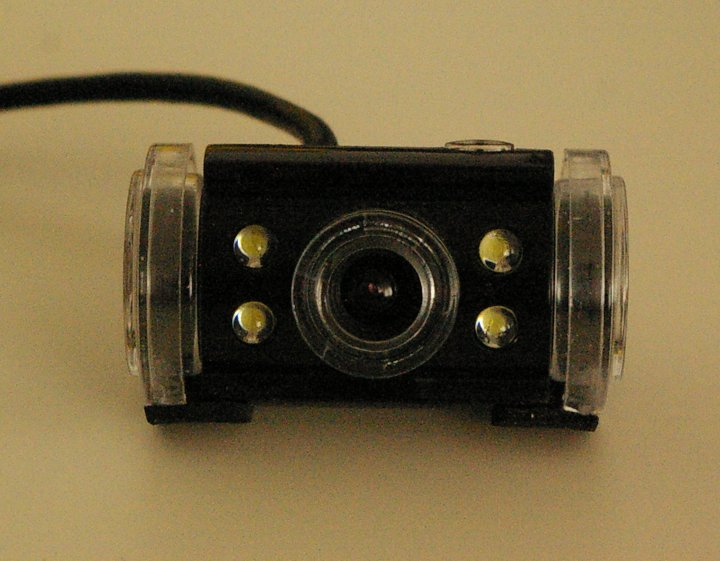
\includegraphics[height=4cm]{imagenes/camara_empleada.jpg}
	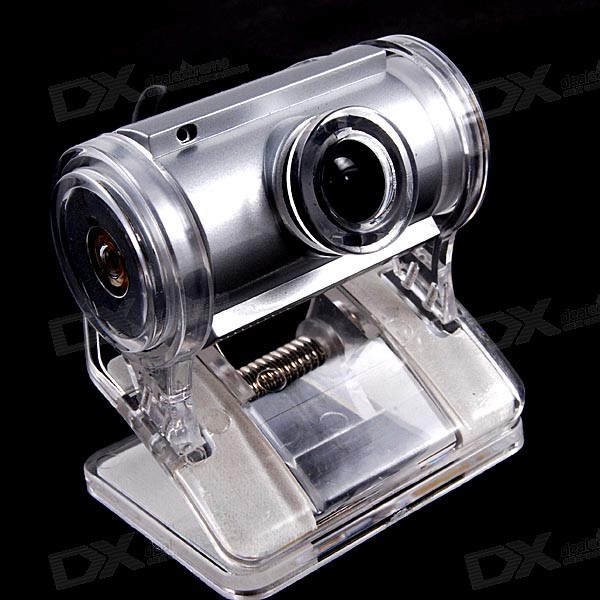
\includegraphics[height=4cm]{imagenes/camara_actual.jpg}
	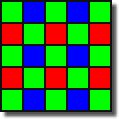
\includegraphics[height=4cm]{imagenes/bayer_mosaic.png}
        \caption{Dispositivo de captura}
	\label{fig:webcam}
\end{figure}

En cuanto a la webcam, se eligió uno de los modelos más económicos que se encontraron. El fabricante comentaba que la cámara tenía 1.3 Megapíxeles, pero se debe tener en cuenta que los fabricantes indican el número de slots que tiene el sensor CMOS como megapíxels. Por cada 4 slots del sensor CMOS (agrupados en grupos de rojo, verde, verde, azul) tenemos un píxel real\footnote{Empleando la interpolación de Bayer, obtenemos un valor BGR de 3 bytes por cada píxel, que luego se convierte a RGB vía software para mostrar por pantalla.} con lo que la resolución real de la cámara es de unos 0,3 megapíxels. Por consiguiente, el tamaño del frame es de 640x480=307200 píxeles de 3 bytes cada uno (para cada uno de los colores indicados). 

En cuanto al resto de las características de la cámara, comentar que tiene incorporado un micrófono que no se ha empleado en ningún momento y que en teoría no ha afectado al desarrollo del proyecto. También hay que tener en cuenta que dicha cámara disponía de iluminación propia (4 leds) que, aunque bastante molesta, daban unas condiciones bastante homogéneas en cuanto a iluminación a costa de en muchos momentos sobreexponer la imagen. Se optó por hacer la mayoría de las pruebas tapando dichos leds con cinta aislante por las molestias que causaban. Actualmente el fabricante ha conservado el soporte de la cámara pero ha retirado los LEDs. También se modificó el soporte de la cámara, recortando y limando el soporte de sujección/pinza que tenía debido a que hacía más complicado el uso de ella. En la figura \ref{fig:webcam} se pueden ver, de izquierda a derecha, la cámara que se ha empleado para hacer las pruebas, el modelo que distribuye actualmente el vendedor (nótese la ausencia de LEDs) y el detalle de un sensor CCD de Webcam económica, donde cada cuadrado 2x2 (colores verde-azul-rojo-verde) corresponde a un píxel.

\subsection{Escenario}
\begin{figure}[h!]
        \centering
        % Graphic for TeX using PGF
% Title: /home/bruno/pfc_UOC/PAC3/pac3/diagramas/Pasos_sistema.dia
% Creator: Dia v0.97
% CreationDate: Thu Apr 22 17:43:32 2010
% For: bruno
% \usepackage{tikz}
% The following commands are not supported in PSTricks at present
% We define them conditionally, so when they are implemented,
% this pgf file will use them.
\ifx\du\undefined
  \newlength{\du}
\fi
\setlength{\du}{15\unitlength}
\begin{tikzpicture}
\pgftransformxscale{1.000000}
\pgftransformyscale{-1.000000}
\definecolor{dialinecolor}{rgb}{0.000000, 0.000000, 0.000000}
\pgfsetstrokecolor{dialinecolor}
\definecolor{dialinecolor}{rgb}{1.000000, 1.000000, 1.000000}
\pgfsetfillcolor{dialinecolor}
\pgfsetlinewidth{0.100000\du}
\pgfsetdash{}{0pt}
\pgfsetdash{}{0pt}
\pgfsetroundjoin
{\pgfsetcornersarced{\pgfpoint{0.300000\du}{0.300000\du}}\definecolor{dialinecolor}{rgb}{0.960784, 0.980392, 0.764706}
\pgfsetfillcolor{dialinecolor}
\fill (3.600000\du,1.200000\du)--(3.600000\du,6.400000\du)--(9.700000\du,6.400000\du)--(9.700000\du,1.200000\du)--cycle;
}{\pgfsetcornersarced{\pgfpoint{0.300000\du}{0.300000\du}}\definecolor{dialinecolor}{rgb}{0.000000, 0.000000, 0.000000}
\pgfsetstrokecolor{dialinecolor}
\draw (3.600000\du,1.200000\du)--(3.600000\du,6.400000\du)--(9.700000\du,6.400000\du)--(9.700000\du,1.200000\du)--cycle;
}\pgfsetlinewidth{0.100000\du}
\pgfsetdash{}{0pt}
\pgfsetdash{}{0pt}
\pgfsetbuttcap
\pgfsetmiterjoin
\pgfsetbuttcap
\pgfsetmiterjoin
\pgfsetdash{}{0pt}
\definecolor{dialinecolor}{rgb}{0.266667, 0.266667, 0.266667}
\pgfsetstrokecolor{dialinecolor}
\pgfpathmoveto{\pgfpoint{7.697270\du}{2.515137\du}}
\pgfpathlineto{\pgfpoint{7.701699\du}{2.535068\du}}
\pgfpathlineto{\pgfpoint{7.707491\du}{2.554828\du}}
\pgfpathlineto{\pgfpoint{7.713793\du}{2.574589\du}}
\pgfpathlineto{\pgfpoint{7.721800\du}{2.594009\du}}
\pgfpathlineto{\pgfpoint{7.730317\du}{2.612406\du}}
\pgfpathlineto{\pgfpoint{7.740027\du}{2.630975\du}}
\pgfpathlineto{\pgfpoint{7.751100\du}{2.648861\du}}
\pgfpathlineto{\pgfpoint{7.762343\du}{2.666237\du}}
\pgfpathlineto{\pgfpoint{7.775119\du}{2.683102\du}}
\pgfpathlineto{\pgfpoint{7.789258\du}{2.699455\du}}
\pgfpathlineto{\pgfpoint{7.803227\du}{2.714957\du}}
\pgfpathlineto{\pgfpoint{7.819069\du}{2.729777\du}}
\pgfpathlineto{\pgfpoint{7.834571\du}{2.744087\du}}
\pgfpathlineto{\pgfpoint{7.852117\du}{2.757204\du}}
\pgfpathlineto{\pgfpoint{7.869323\du}{2.769980\du}}
\pgfpathlineto{\pgfpoint{7.887720\du}{2.781904\du}}
\pgfpathlineto{\pgfpoint{7.906970\du}{2.792807\du}}
\pgfpathlineto{\pgfpoint{7.926730\du}{2.802687\du}}
\pgfpathlineto{\pgfpoint{7.946661\du}{2.812056\du}}
\pgfpathlineto{\pgfpoint{7.967274\du}{2.820233\du}}
\pgfpathlineto{\pgfpoint{7.987886\du}{2.827388\du}}
\pgfpathlineto{\pgfpoint{8.009691\du}{2.833861\du}}
\pgfpathlineto{\pgfpoint{8.031325\du}{2.839142\du}}
\pgfpathlineto{\pgfpoint{8.053470\du}{2.843400\du}}
\pgfpathlineto{\pgfpoint{8.075445\du}{2.846637\du}}
\pgfpathlineto{\pgfpoint{8.097932\du}{2.849192\du}}
\pgfpathlineto{\pgfpoint{8.120588\du}{2.850214\du}}
\pgfpathlineto{\pgfpoint{8.142904\du}{2.850555\du}}
\pgfpathlineto{\pgfpoint{8.165390\du}{2.849533\du}}
\pgfpathlineto{\pgfpoint{8.187535\du}{2.847489\du}}
\pgfpathlineto{\pgfpoint{8.210022\du}{2.844934\du}}
\pgfpathlineto{\pgfpoint{8.232337\du}{2.841186\du}}
\pgfpathlineto{\pgfpoint{8.253631\du}{2.836246\du}}
\pgfpathlineto{\pgfpoint{8.275095\du}{2.830283\du}}
\pgfpathlineto{\pgfpoint{8.296218\du}{2.823129\du}}
\pgfpathlineto{\pgfpoint{8.317171\du}{2.815633\du}}
\pgfpathlineto{\pgfpoint{8.337784\du}{2.806946\du}}
\pgfpathlineto{\pgfpoint{8.357544\du}{2.797065\du}}
\pgfpathlineto{\pgfpoint{8.376453\du}{2.786504\du}}
\pgfpathlineto{\pgfpoint{8.395362\du}{2.775090\du}}
\pgfpathlineto{\pgfpoint{8.413249\du}{2.762825\du}}
\pgfpathlineto{\pgfpoint{8.430624\du}{2.749708\du}}
\pgfpathlineto{\pgfpoint{8.447148\du}{2.735739\du}}
\pgfpathlineto{\pgfpoint{8.462650\du}{2.721260\du}}
\pgfpathlineto{\pgfpoint{8.477641\du}{2.705928\du}}
\pgfpathlineto{\pgfpoint{8.491780\du}{2.689915\du}}
\pgfpathlineto{\pgfpoint{8.504897\du}{2.673562\du}}
\pgfpathlineto{\pgfpoint{8.516991\du}{2.656357\du}}
\pgfpathlineto{\pgfpoint{8.528405\du}{2.638470\du}}
\pgfpathlineto{\pgfpoint{8.537944\du}{2.620413\du}}
\pgfpathlineto{\pgfpoint{8.547654\du}{2.601504\du}}
\pgfpathlineto{\pgfpoint{8.556001\du}{2.582936\du}}
\pgfpathlineto{\pgfpoint{8.562645\du}{2.563175\du}}
\pgfpathlineto{\pgfpoint{8.568948\du}{2.543585\du}}
\pgfpathlineto{\pgfpoint{8.573718\du}{2.523825\du}}
\pgfusepath{stroke}
\pgfsetlinewidth{0.030000\du}
\pgfsetbuttcap
\pgfsetmiterjoin
\pgfsetdash{}{0pt}
\definecolor{dialinecolor}{rgb}{0.133333, 0.133333, 0.133333}
\pgfsetfillcolor{dialinecolor}
\pgfpathmoveto{\pgfpoint{8.516480\du}{2.379879\du}}
\pgfpathlineto{\pgfpoint{8.515799\du}{2.360630\du}}
\pgfpathlineto{\pgfpoint{8.514606\du}{2.341380\du}}
\pgfpathlineto{\pgfpoint{8.512051\du}{2.322472\du}}
\pgfpathlineto{\pgfpoint{8.508474\du}{2.303392\du}}
\pgfpathlineto{\pgfpoint{8.504045\du}{2.284484\du}}
\pgfpathlineto{\pgfpoint{8.498934\du}{2.266086\du}}
\pgfpathlineto{\pgfpoint{8.492802\du}{2.247859\du}}
\pgfpathlineto{\pgfpoint{8.485477\du}{2.229972\du}}
\pgfpathlineto{\pgfpoint{8.477470\du}{2.212767\du}}
\pgfpathlineto{\pgfpoint{8.468612\du}{2.195561\du}}
\pgfpathlineto{\pgfpoint{8.458902\du}{2.178867\du}}
\pgfpathlineto{\pgfpoint{8.448341\du}{2.162854\du}}
\pgfpathlineto{\pgfpoint{8.436757\du}{2.147352\du}}
\pgfpathlineto{\pgfpoint{8.424662\du}{2.132532\du}}
\pgfpathlineto{\pgfpoint{8.411545\du}{2.118052\du}}
\pgfpathlineto{\pgfpoint{8.398258\du}{2.104424\du}}
\pgfpathlineto{\pgfpoint{8.383778\du}{2.091478\du}}
\pgfpathlineto{\pgfpoint{8.368787\du}{2.079553\du}}
\pgfpathlineto{\pgfpoint{8.353456\du}{2.067969\du}}
\pgfpathlineto{\pgfpoint{8.337613\du}{2.057408\du}}
\pgfpathlineto{\pgfpoint{8.320749\du}{2.047868\du}}
\pgfpathlineto{\pgfpoint{8.303714\du}{2.039010\du}}
\pgfpathlineto{\pgfpoint{8.286338\du}{2.030833\du}}
\pgfpathlineto{\pgfpoint{8.268622\du}{2.023508\du}}
\pgfpathlineto{\pgfpoint{8.250224\du}{2.017205\du}}
\pgfpathlineto{\pgfpoint{8.231656\du}{2.012265\du}}
\pgfpathlineto{\pgfpoint{8.213088\du}{2.007666\du}}
\pgfpathlineto{\pgfpoint{8.194009\du}{2.004259\du}}
\pgfpathlineto{\pgfpoint{8.174930\du}{2.001874\du}}
\pgfpathlineto{\pgfpoint{8.155680\du}{2.000511\du}}
\pgfpathlineto{\pgfpoint{8.136601\du}{2.000000\du}}
\pgfpathlineto{\pgfpoint{8.136601\du}{2.000000\du}}
\pgfpathlineto{\pgfpoint{8.117351\du}{2.000511\du}}
\pgfpathlineto{\pgfpoint{8.098102\du}{2.001874\du}}
\pgfpathlineto{\pgfpoint{8.079023\du}{2.004259\du}}
\pgfpathlineto{\pgfpoint{8.059944\du}{2.007666\du}}
\pgfpathlineto{\pgfpoint{8.041035\du}{2.012265\du}}
\pgfpathlineto{\pgfpoint{8.022637\du}{2.017205\du}}
\pgfpathlineto{\pgfpoint{8.004580\du}{2.023508\du}}
\pgfpathlineto{\pgfpoint{7.986523\du}{2.030833\du}}
\pgfpathlineto{\pgfpoint{7.969147\du}{2.039010\du}}
\pgfpathlineto{\pgfpoint{7.952112\du}{2.047868\du}}
\pgfpathlineto{\pgfpoint{7.935248\du}{2.057408\du}}
\pgfpathlineto{\pgfpoint{7.919405\du}{2.067969\du}}
\pgfpathlineto{\pgfpoint{7.904074\du}{2.079553\du}}
\pgfpathlineto{\pgfpoint{7.889083\du}{2.091478\du}}
\pgfpathlineto{\pgfpoint{7.874603\du}{2.104424\du}}
\pgfpathlineto{\pgfpoint{7.861146\du}{2.118052\du}}
\pgfpathlineto{\pgfpoint{7.848199\du}{2.132532\du}}
\pgfpathlineto{\pgfpoint{7.836275\du}{2.147352\du}}
\pgfpathlineto{\pgfpoint{7.824521\du}{2.162854\du}}
\pgfpathlineto{\pgfpoint{7.814129\du}{2.178867\du}}
\pgfpathlineto{\pgfpoint{7.804419\du}{2.195561\du}}
\pgfpathlineto{\pgfpoint{7.795391\du}{2.212767\du}}
\pgfpathlineto{\pgfpoint{7.787384\du}{2.229972\du}}
\pgfpathlineto{\pgfpoint{7.780230\du}{2.247859\du}}
\pgfpathlineto{\pgfpoint{7.773927\du}{2.266086\du}}
\pgfpathlineto{\pgfpoint{7.768646\du}{2.284484\du}}
\pgfpathlineto{\pgfpoint{7.764387\du}{2.303392\du}}
\pgfpathlineto{\pgfpoint{7.761151\du}{2.322472\du}}
\pgfpathlineto{\pgfpoint{7.758595\du}{2.341380\du}}
\pgfpathlineto{\pgfpoint{7.756892\du}{2.360630\du}}
\pgfpathlineto{\pgfpoint{7.756551\du}{2.379879\du}}
\pgfpathlineto{\pgfpoint{7.756551\du}{2.379879\du}}
\pgfpathlineto{\pgfpoint{7.756892\du}{2.399129\du}}
\pgfpathlineto{\pgfpoint{7.758595\du}{2.418378\du}}
\pgfpathlineto{\pgfpoint{7.761151\du}{2.437287\du}}
\pgfpathlineto{\pgfpoint{7.764387\du}{2.456366\du}}
\pgfpathlineto{\pgfpoint{7.768646\du}{2.474934\du}}
\pgfpathlineto{\pgfpoint{7.773927\du}{2.493673\du}}
\pgfpathlineto{\pgfpoint{7.780230\du}{2.511900\du}}
\pgfpathlineto{\pgfpoint{7.787384\du}{2.529787\du}}
\pgfpathlineto{\pgfpoint{7.795391\du}{2.547163\du}}
\pgfpathlineto{\pgfpoint{7.804419\du}{2.564198\du}}
\pgfpathlineto{\pgfpoint{7.814129\du}{2.580892\du}}
\pgfpathlineto{\pgfpoint{7.824521\du}{2.596734\du}}
\pgfpathlineto{\pgfpoint{7.836275\du}{2.612406\du}}
\pgfpathlineto{\pgfpoint{7.848199\du}{2.627057\du}}
\pgfpathlineto{\pgfpoint{7.861146\du}{2.641536\du}}
\pgfpathlineto{\pgfpoint{7.874603\du}{2.654994\du}}
\pgfpathlineto{\pgfpoint{7.889083\du}{2.668111\du}}
\pgfpathlineto{\pgfpoint{7.904074\du}{2.680206\du}}
\pgfpathlineto{\pgfpoint{7.919405\du}{2.691789\du}}
\pgfpathlineto{\pgfpoint{7.935248\du}{2.702351\du}}
\pgfpathlineto{\pgfpoint{7.952112\du}{2.711891\du}}
\pgfpathlineto{\pgfpoint{7.969147\du}{2.720749\du}}
\pgfpathlineto{\pgfpoint{7.986523\du}{2.729096\du}}
\pgfpathlineto{\pgfpoint{8.004580\du}{2.735910\du}}
\pgfpathlineto{\pgfpoint{8.022637\du}{2.742213\du}}
\pgfpathlineto{\pgfpoint{8.041035\du}{2.747494\du}}
\pgfpathlineto{\pgfpoint{8.059944\du}{2.752093\du}}
\pgfpathlineto{\pgfpoint{8.079023\du}{2.755330\du}}
\pgfpathlineto{\pgfpoint{8.098102\du}{2.757885\du}}
\pgfpathlineto{\pgfpoint{8.117351\du}{2.759077\du}}
\pgfpathlineto{\pgfpoint{8.136601\du}{2.759759\du}}
\pgfpathlineto{\pgfpoint{8.136601\du}{2.759759\du}}
\pgfpathlineto{\pgfpoint{8.155680\du}{2.759077\du}}
\pgfpathlineto{\pgfpoint{8.174930\du}{2.757885\du}}
\pgfpathlineto{\pgfpoint{8.194009\du}{2.755330\du}}
\pgfpathlineto{\pgfpoint{8.213088\du}{2.752093\du}}
\pgfpathlineto{\pgfpoint{8.231656\du}{2.747494\du}}
\pgfpathlineto{\pgfpoint{8.250224\du}{2.742213\du}}
\pgfpathlineto{\pgfpoint{8.268622\du}{2.735910\du}}
\pgfpathlineto{\pgfpoint{8.286338\du}{2.729096\du}}
\pgfpathlineto{\pgfpoint{8.303714\du}{2.720749\du}}
\pgfpathlineto{\pgfpoint{8.320749\du}{2.711891\du}}
\pgfpathlineto{\pgfpoint{8.337613\du}{2.702351\du}}
\pgfpathlineto{\pgfpoint{8.353456\du}{2.691789\du}}
\pgfpathlineto{\pgfpoint{8.368787\du}{2.680206\du}}
\pgfpathlineto{\pgfpoint{8.383778\du}{2.668111\du}}
\pgfpathlineto{\pgfpoint{8.398258\du}{2.654994\du}}
\pgfpathlineto{\pgfpoint{8.411545\du}{2.641536\du}}
\pgfpathlineto{\pgfpoint{8.424662\du}{2.627057\du}}
\pgfpathlineto{\pgfpoint{8.436757\du}{2.612406\du}}
\pgfpathlineto{\pgfpoint{8.448341\du}{2.596734\du}}
\pgfpathlineto{\pgfpoint{8.458902\du}{2.580892\du}}
\pgfpathlineto{\pgfpoint{8.468612\du}{2.564198\du}}
\pgfpathlineto{\pgfpoint{8.477470\du}{2.547163\du}}
\pgfpathlineto{\pgfpoint{8.485477\du}{2.529787\du}}
\pgfpathlineto{\pgfpoint{8.492802\du}{2.511900\du}}
\pgfpathlineto{\pgfpoint{8.498934\du}{2.493673\du}}
\pgfpathlineto{\pgfpoint{8.504045\du}{2.474934\du}}
\pgfpathlineto{\pgfpoint{8.508474\du}{2.456366\du}}
\pgfpathlineto{\pgfpoint{8.512051\du}{2.437287\du}}
\pgfpathlineto{\pgfpoint{8.514606\du}{2.418378\du}}
\pgfpathlineto{\pgfpoint{8.515799\du}{2.399129\du}}
\pgfpathlineto{\pgfpoint{8.516480\du}{2.379879\du}}
\pgfusepath{fill}
\pgfsetbuttcap
\pgfsetmiterjoin
\pgfsetdash{}{0pt}
\definecolor{dialinecolor}{rgb}{0.223529, 0.223529, 0.223529}
\pgfsetfillcolor{dialinecolor}
\pgfpathmoveto{\pgfpoint{8.507963\du}{2.371532\du}}
\pgfpathlineto{\pgfpoint{8.507281\du}{2.352964\du}}
\pgfpathlineto{\pgfpoint{8.506089\du}{2.334737\du}}
\pgfpathlineto{\pgfpoint{8.503704\du}{2.316169\du}}
\pgfpathlineto{\pgfpoint{8.500467\du}{2.298112\du}}
\pgfpathlineto{\pgfpoint{8.496209\du}{2.280055\du}}
\pgfpathlineto{\pgfpoint{8.491269\du}{2.262679\du}}
\pgfpathlineto{\pgfpoint{8.485306\du}{2.245303\du}}
\pgfpathlineto{\pgfpoint{8.478322\du}{2.228268\du}}
\pgfpathlineto{\pgfpoint{8.470827\du}{2.211233\du}}
\pgfpathlineto{\pgfpoint{8.462309\du}{2.194880\du}}
\pgfpathlineto{\pgfpoint{8.452770\du}{2.179037\du}}
\pgfpathlineto{\pgfpoint{8.442889\du}{2.163876\du}}
\pgfpathlineto{\pgfpoint{8.431817\du}{2.148885\du}}
\pgfpathlineto{\pgfpoint{8.420403\du}{2.134576\du}}
\pgfpathlineto{\pgfpoint{8.407968\du}{2.121118\du}}
\pgfpathlineto{\pgfpoint{8.395021\du}{2.108172\du}}
\pgfpathlineto{\pgfpoint{8.381393\du}{2.095736\du}}
\pgfpathlineto{\pgfpoint{8.366913\du}{2.083982\du}}
\pgfpathlineto{\pgfpoint{8.352263\du}{2.073250\du}}
\pgfpathlineto{\pgfpoint{8.336762\du}{2.063029\du}}
\pgfpathlineto{\pgfpoint{8.320749\du}{2.053660\du}}
\pgfpathlineto{\pgfpoint{8.304566\du}{2.045143\du}}
\pgfpathlineto{\pgfpoint{8.287871\du}{2.037307\du}}
\pgfpathlineto{\pgfpoint{8.270666\du}{2.030493\du}}
\pgfpathlineto{\pgfpoint{8.253631\du}{2.024530\du}}
\pgfpathlineto{\pgfpoint{8.235574\du}{2.019249\du}}
\pgfpathlineto{\pgfpoint{8.217517\du}{2.015502\du}}
\pgfpathlineto{\pgfpoint{8.199630\du}{2.012265\du}}
\pgfpathlineto{\pgfpoint{8.181232\du}{2.009710\du}}
\pgfpathlineto{\pgfpoint{8.163175\du}{2.008517\du}}
\pgfpathlineto{\pgfpoint{8.144778\du}{2.008006\du}}
\pgfpathlineto{\pgfpoint{8.144778\du}{2.008006\du}}
\pgfpathlineto{\pgfpoint{8.126039\du}{2.008517\du}}
\pgfpathlineto{\pgfpoint{8.107812\du}{2.009710\du}}
\pgfpathlineto{\pgfpoint{8.089755\du}{2.012265\du}}
\pgfpathlineto{\pgfpoint{8.071698\du}{2.015502\du}}
\pgfpathlineto{\pgfpoint{8.053470\du}{2.019249\du}}
\pgfpathlineto{\pgfpoint{8.035754\du}{2.024530\du}}
\pgfpathlineto{\pgfpoint{8.018378\du}{2.030493\du}}
\pgfpathlineto{\pgfpoint{8.001343\du}{2.037307\du}}
\pgfpathlineto{\pgfpoint{7.984649\du}{2.045143\du}}
\pgfpathlineto{\pgfpoint{7.968296\du}{2.053660\du}}
\pgfpathlineto{\pgfpoint{7.952453\du}{2.063029\du}}
\pgfpathlineto{\pgfpoint{7.937122\du}{2.073250\du}}
\pgfpathlineto{\pgfpoint{7.922301\du}{2.083982\du}}
\pgfpathlineto{\pgfpoint{7.907992\du}{2.095736\du}}
\pgfpathlineto{\pgfpoint{7.894534\du}{2.108172\du}}
\pgfpathlineto{\pgfpoint{7.881247\du}{2.121118\du}}
\pgfpathlineto{\pgfpoint{7.868982\du}{2.134576\du}}
\pgfpathlineto{\pgfpoint{7.857568\du}{2.148885\du}}
\pgfpathlineto{\pgfpoint{7.846496\du}{2.163876\du}}
\pgfpathlineto{\pgfpoint{7.836275\du}{2.179037\du}}
\pgfpathlineto{\pgfpoint{7.826906\du}{2.194880\du}}
\pgfpathlineto{\pgfpoint{7.818558\du}{2.211233\du}}
\pgfpathlineto{\pgfpoint{7.810722\du}{2.228268\du}}
\pgfpathlineto{\pgfpoint{7.804079\du}{2.245303\du}}
\pgfpathlineto{\pgfpoint{7.797946\du}{2.262679\du}}
\pgfpathlineto{\pgfpoint{7.793176\du}{2.280055\du}}
\pgfpathlineto{\pgfpoint{7.788918\du}{2.298112\du}}
\pgfpathlineto{\pgfpoint{7.785681\du}{2.316169\du}}
\pgfpathlineto{\pgfpoint{7.783126\du}{2.334737\du}}
\pgfpathlineto{\pgfpoint{7.781933\du}{2.352964\du}}
\pgfpathlineto{\pgfpoint{7.781422\du}{2.371532\du}}
\pgfpathlineto{\pgfpoint{7.781422\du}{2.371532\du}}
\pgfpathlineto{\pgfpoint{7.781933\du}{2.389760\du}}
\pgfpathlineto{\pgfpoint{7.783126\du}{2.408328\du}}
\pgfpathlineto{\pgfpoint{7.785681\du}{2.426555\du}}
\pgfpathlineto{\pgfpoint{7.788918\du}{2.444612\du}}
\pgfpathlineto{\pgfpoint{7.793176\du}{2.462669\du}}
\pgfpathlineto{\pgfpoint{7.797946\du}{2.480215\du}}
\pgfpathlineto{\pgfpoint{7.804079\du}{2.497421\du}}
\pgfpathlineto{\pgfpoint{7.810722\du}{2.514796\du}}
\pgfpathlineto{\pgfpoint{7.818558\du}{2.531490\du}}
\pgfpathlineto{\pgfpoint{7.826906\du}{2.547844\du}}
\pgfpathlineto{\pgfpoint{7.836275\du}{2.563686\du}}
\pgfpathlineto{\pgfpoint{7.846496\du}{2.579018\du}}
\pgfpathlineto{\pgfpoint{7.857568\du}{2.594009\du}}
\pgfpathlineto{\pgfpoint{7.868982\du}{2.608148\du}}
\pgfpathlineto{\pgfpoint{7.881247\du}{2.621776\du}}
\pgfpathlineto{\pgfpoint{7.894534\du}{2.634552\du}}
\pgfpathlineto{\pgfpoint{7.907992\du}{2.647158\du}}
\pgfpathlineto{\pgfpoint{7.922301\du}{2.658912\du}}
\pgfpathlineto{\pgfpoint{7.937122\du}{2.669644\du}}
\pgfpathlineto{\pgfpoint{7.952453\du}{2.679865\du}}
\pgfpathlineto{\pgfpoint{7.968296\du}{2.689064\du}}
\pgfpathlineto{\pgfpoint{7.984649\du}{2.697922\du}}
\pgfpathlineto{\pgfpoint{8.001343\du}{2.705417\du}}
\pgfpathlineto{\pgfpoint{8.018378\du}{2.712231\du}}
\pgfpathlineto{\pgfpoint{8.035754\du}{2.718193\du}}
\pgfpathlineto{\pgfpoint{8.053470\du}{2.723474\du}}
\pgfpathlineto{\pgfpoint{8.071698\du}{2.727222\du}}
\pgfpathlineto{\pgfpoint{8.089755\du}{2.730459\du}}
\pgfpathlineto{\pgfpoint{8.107812\du}{2.733014\du}}
\pgfpathlineto{\pgfpoint{8.126039\du}{2.734377\du}}
\pgfpathlineto{\pgfpoint{8.144778\du}{2.734717\du}}
\pgfpathlineto{\pgfpoint{8.144778\du}{2.734717\du}}
\pgfpathlineto{\pgfpoint{8.163175\du}{2.734377\du}}
\pgfpathlineto{\pgfpoint{8.181232\du}{2.733014\du}}
\pgfpathlineto{\pgfpoint{8.199630\du}{2.730459\du}}
\pgfpathlineto{\pgfpoint{8.217517\du}{2.727222\du}}
\pgfpathlineto{\pgfpoint{8.235574\du}{2.723474\du}}
\pgfpathlineto{\pgfpoint{8.253631\du}{2.718193\du}}
\pgfpathlineto{\pgfpoint{8.270666\du}{2.712231\du}}
\pgfpathlineto{\pgfpoint{8.287871\du}{2.705417\du}}
\pgfpathlineto{\pgfpoint{8.304566\du}{2.697922\du}}
\pgfpathlineto{\pgfpoint{8.320749\du}{2.689064\du}}
\pgfpathlineto{\pgfpoint{8.336762\du}{2.679865\du}}
\pgfpathlineto{\pgfpoint{8.352263\du}{2.669644\du}}
\pgfpathlineto{\pgfpoint{8.366913\du}{2.658912\du}}
\pgfpathlineto{\pgfpoint{8.381393\du}{2.647158\du}}
\pgfpathlineto{\pgfpoint{8.395021\du}{2.634552\du}}
\pgfpathlineto{\pgfpoint{8.407968\du}{2.621776\du}}
\pgfpathlineto{\pgfpoint{8.420403\du}{2.608148\du}}
\pgfpathlineto{\pgfpoint{8.431817\du}{2.594009\du}}
\pgfpathlineto{\pgfpoint{8.442889\du}{2.579018\du}}
\pgfpathlineto{\pgfpoint{8.452770\du}{2.563686\du}}
\pgfpathlineto{\pgfpoint{8.462309\du}{2.547844\du}}
\pgfpathlineto{\pgfpoint{8.470827\du}{2.531490\du}}
\pgfpathlineto{\pgfpoint{8.478322\du}{2.514796\du}}
\pgfpathlineto{\pgfpoint{8.485306\du}{2.497421\du}}
\pgfpathlineto{\pgfpoint{8.491269\du}{2.480215\du}}
\pgfpathlineto{\pgfpoint{8.496209\du}{2.462669\du}}
\pgfpathlineto{\pgfpoint{8.500467\du}{2.444612\du}}
\pgfpathlineto{\pgfpoint{8.503704\du}{2.426555\du}}
\pgfpathlineto{\pgfpoint{8.506089\du}{2.408328\du}}
\pgfpathlineto{\pgfpoint{8.507281\du}{2.389760\du}}
\pgfpathlineto{\pgfpoint{8.507963\du}{2.371532\du}}
\pgfusepath{fill}
\pgfsetbuttcap
\pgfsetmiterjoin
\pgfsetdash{}{0pt}
\definecolor{dialinecolor}{rgb}{0.317647, 0.317647, 0.317647}
\pgfsetfillcolor{dialinecolor}
\pgfpathmoveto{\pgfpoint{8.499616\du}{2.358926\du}}
\pgfpathlineto{\pgfpoint{8.498934\du}{2.341721\du}}
\pgfpathlineto{\pgfpoint{8.497572\du}{2.324345\du}}
\pgfpathlineto{\pgfpoint{8.495357\du}{2.307140\du}}
\pgfpathlineto{\pgfpoint{8.492461\du}{2.290105\du}}
\pgfpathlineto{\pgfpoint{8.488543\du}{2.273241\du}}
\pgfpathlineto{\pgfpoint{8.483603\du}{2.256376\du}}
\pgfpathlineto{\pgfpoint{8.477981\du}{2.239682\du}}
\pgfpathlineto{\pgfpoint{8.471508\du}{2.223499\du}}
\pgfpathlineto{\pgfpoint{8.464183\du}{2.207826\du}}
\pgfpathlineto{\pgfpoint{8.456006\du}{2.192495\du}}
\pgfpathlineto{\pgfpoint{8.447148\du}{2.177675\du}}
\pgfpathlineto{\pgfpoint{8.437608\du}{2.163024\du}}
\pgfpathlineto{\pgfpoint{8.427047\du}{2.149056\du}}
\pgfpathlineto{\pgfpoint{8.415804\du}{2.135769\du}}
\pgfpathlineto{\pgfpoint{8.403879\du}{2.122992\du}}
\pgfpathlineto{\pgfpoint{8.391614\du}{2.110557\du}}
\pgfpathlineto{\pgfpoint{8.378838\du}{2.098973\du}}
\pgfpathlineto{\pgfpoint{8.365210\du}{2.087900\du}}
\pgfpathlineto{\pgfpoint{8.350730\du}{2.077679\du}}
\pgfpathlineto{\pgfpoint{8.336251\du}{2.067969\du}}
\pgfpathlineto{\pgfpoint{8.321089\du}{2.059452\du}}
\pgfpathlineto{\pgfpoint{8.305588\du}{2.051105\du}}
\pgfpathlineto{\pgfpoint{8.289575\du}{2.043780\du}}
\pgfpathlineto{\pgfpoint{8.273051\du}{2.037307\du}}
\pgfpathlineto{\pgfpoint{8.256527\du}{2.031855\du}}
\pgfpathlineto{\pgfpoint{8.239833\du}{2.027256\du}}
\pgfpathlineto{\pgfpoint{8.222627\du}{2.023338\du}}
\pgfpathlineto{\pgfpoint{8.205422\du}{2.020101\du}}
\pgfpathlineto{\pgfpoint{8.187876\du}{2.018057\du}}
\pgfpathlineto{\pgfpoint{8.170500\du}{2.016694\du}}
\pgfpathlineto{\pgfpoint{8.152784\du}{2.016013\du}}
\pgfpathlineto{\pgfpoint{8.152784\du}{2.016013\du}}
\pgfpathlineto{\pgfpoint{8.135408\du}{2.016694\du}}
\pgfpathlineto{\pgfpoint{8.117692\du}{2.018057\du}}
\pgfpathlineto{\pgfpoint{8.100316\du}{2.020101\du}}
\pgfpathlineto{\pgfpoint{8.083111\du}{2.023338\du}}
\pgfpathlineto{\pgfpoint{8.066076\du}{2.027256\du}}
\pgfpathlineto{\pgfpoint{8.049212\du}{2.031855\du}}
\pgfpathlineto{\pgfpoint{8.032517\du}{2.037307\du}}
\pgfpathlineto{\pgfpoint{8.016164\du}{2.043780\du}}
\pgfpathlineto{\pgfpoint{8.000321\du}{2.051105\du}}
\pgfpathlineto{\pgfpoint{7.984479\du}{2.059452\du}}
\pgfpathlineto{\pgfpoint{7.969488\du}{2.067969\du}}
\pgfpathlineto{\pgfpoint{7.954668\du}{2.077679\du}}
\pgfpathlineto{\pgfpoint{7.940699\du}{2.087900\du}}
\pgfpathlineto{\pgfpoint{7.926901\du}{2.098973\du}}
\pgfpathlineto{\pgfpoint{7.913954\du}{2.110557\du}}
\pgfpathlineto{\pgfpoint{7.901519\du}{2.122992\du}}
\pgfpathlineto{\pgfpoint{7.889594\du}{2.135769\du}}
\pgfpathlineto{\pgfpoint{7.878862\du}{2.149056\du}}
\pgfpathlineto{\pgfpoint{7.868300\du}{2.163024\du}}
\pgfpathlineto{\pgfpoint{7.858591\du}{2.177675\du}}
\pgfpathlineto{\pgfpoint{7.849732\du}{2.192495\du}}
\pgfpathlineto{\pgfpoint{7.841556\du}{2.207826\du}}
\pgfpathlineto{\pgfpoint{7.834231\du}{2.223499\du}}
\pgfpathlineto{\pgfpoint{7.827757\du}{2.239682\du}}
\pgfpathlineto{\pgfpoint{7.822136\du}{2.256376\du}}
\pgfpathlineto{\pgfpoint{7.817196\du}{2.273241\du}}
\pgfpathlineto{\pgfpoint{7.813107\du}{2.290105\du}}
\pgfpathlineto{\pgfpoint{7.810041\du}{2.307140\du}}
\pgfpathlineto{\pgfpoint{7.808167\du}{2.324345\du}}
\pgfpathlineto{\pgfpoint{7.806634\du}{2.341721\du}}
\pgfpathlineto{\pgfpoint{7.806293\du}{2.358926\du}}
\pgfpathlineto{\pgfpoint{7.806293\du}{2.358926\du}}
\pgfpathlineto{\pgfpoint{7.806634\du}{2.376472\du}}
\pgfpathlineto{\pgfpoint{7.808167\du}{2.393678\du}}
\pgfpathlineto{\pgfpoint{7.810041\du}{2.410883\du}}
\pgfpathlineto{\pgfpoint{7.813107\du}{2.427918\du}}
\pgfpathlineto{\pgfpoint{7.817196\du}{2.444783\du}}
\pgfpathlineto{\pgfpoint{7.822136\du}{2.461817\du}}
\pgfpathlineto{\pgfpoint{7.827757\du}{2.478001\du}}
\pgfpathlineto{\pgfpoint{7.834231\du}{2.494184\du}}
\pgfpathlineto{\pgfpoint{7.841556\du}{2.510026\du}}
\pgfpathlineto{\pgfpoint{7.849732\du}{2.525528\du}}
\pgfpathlineto{\pgfpoint{7.858591\du}{2.540349\du}}
\pgfpathlineto{\pgfpoint{7.868300\du}{2.554658\du}}
\pgfpathlineto{\pgfpoint{7.878862\du}{2.568967\du}}
\pgfpathlineto{\pgfpoint{7.889594\du}{2.582255\du}}
\pgfpathlineto{\pgfpoint{7.901519\du}{2.595201\du}}
\pgfpathlineto{\pgfpoint{7.913954\du}{2.607637\du}}
\pgfpathlineto{\pgfpoint{7.926901\du}{2.619050\du}}
\pgfpathlineto{\pgfpoint{7.940699\du}{2.630123\du}}
\pgfpathlineto{\pgfpoint{7.954668\du}{2.640344\du}}
\pgfpathlineto{\pgfpoint{7.969488\du}{2.650054\du}}
\pgfpathlineto{\pgfpoint{7.984479\du}{2.658742\du}}
\pgfpathlineto{\pgfpoint{8.000321\du}{2.666918\du}}
\pgfpathlineto{\pgfpoint{8.016164\du}{2.674073\du}}
\pgfpathlineto{\pgfpoint{8.032517\du}{2.680376\du}}
\pgfpathlineto{\pgfpoint{8.049212\du}{2.686168\du}}
\pgfpathlineto{\pgfpoint{8.066076\du}{2.690767\du}}
\pgfpathlineto{\pgfpoint{8.083111\du}{2.694856\du}}
\pgfpathlineto{\pgfpoint{8.100316\du}{2.697922\du}}
\pgfpathlineto{\pgfpoint{8.117692\du}{2.699966\du}}
\pgfpathlineto{\pgfpoint{8.135408\du}{2.701329\du}}
\pgfpathlineto{\pgfpoint{8.152784\du}{2.701670\du}}
\pgfpathlineto{\pgfpoint{8.152784\du}{2.701670\du}}
\pgfpathlineto{\pgfpoint{8.170500\du}{2.701329\du}}
\pgfpathlineto{\pgfpoint{8.187876\du}{2.699966\du}}
\pgfpathlineto{\pgfpoint{8.205422\du}{2.697922\du}}
\pgfpathlineto{\pgfpoint{8.222627\du}{2.694856\du}}
\pgfpathlineto{\pgfpoint{8.239833\du}{2.690767\du}}
\pgfpathlineto{\pgfpoint{8.256527\du}{2.686168\du}}
\pgfpathlineto{\pgfpoint{8.273051\du}{2.680376\du}}
\pgfpathlineto{\pgfpoint{8.289575\du}{2.674073\du}}
\pgfpathlineto{\pgfpoint{8.305588\du}{2.666918\du}}
\pgfpathlineto{\pgfpoint{8.321089\du}{2.658742\du}}
\pgfpathlineto{\pgfpoint{8.336251\du}{2.650054\du}}
\pgfpathlineto{\pgfpoint{8.350730\du}{2.640344\du}}
\pgfpathlineto{\pgfpoint{8.365210\du}{2.630123\du}}
\pgfpathlineto{\pgfpoint{8.378838\du}{2.619050\du}}
\pgfpathlineto{\pgfpoint{8.391614\du}{2.607637\du}}
\pgfpathlineto{\pgfpoint{8.403879\du}{2.595201\du}}
\pgfpathlineto{\pgfpoint{8.415804\du}{2.582255\du}}
\pgfpathlineto{\pgfpoint{8.427047\du}{2.568967\du}}
\pgfpathlineto{\pgfpoint{8.437608\du}{2.554658\du}}
\pgfpathlineto{\pgfpoint{8.447148\du}{2.540349\du}}
\pgfpathlineto{\pgfpoint{8.456006\du}{2.525528\du}}
\pgfpathlineto{\pgfpoint{8.464183\du}{2.510026\du}}
\pgfpathlineto{\pgfpoint{8.471508\du}{2.494184\du}}
\pgfpathlineto{\pgfpoint{8.477981\du}{2.478001\du}}
\pgfpathlineto{\pgfpoint{8.483603\du}{2.461817\du}}
\pgfpathlineto{\pgfpoint{8.488543\du}{2.444783\du}}
\pgfpathlineto{\pgfpoint{8.492461\du}{2.427918\du}}
\pgfpathlineto{\pgfpoint{8.495357\du}{2.410883\du}}
\pgfpathlineto{\pgfpoint{8.497572\du}{2.393678\du}}
\pgfpathlineto{\pgfpoint{8.498934\du}{2.376472\du}}
\pgfpathlineto{\pgfpoint{8.499616\du}{2.358926\du}}
\pgfusepath{fill}
\pgfsetbuttcap
\pgfsetmiterjoin
\pgfsetdash{}{0pt}
\definecolor{dialinecolor}{rgb}{0.403922, 0.403922, 0.403922}
\pgfsetfillcolor{dialinecolor}
\pgfpathmoveto{\pgfpoint{8.483433\du}{2.346661\du}}
\pgfpathlineto{\pgfpoint{8.482751\du}{2.329967\du}}
\pgfpathlineto{\pgfpoint{8.481559\du}{2.313954\du}}
\pgfpathlineto{\pgfpoint{8.479514\du}{2.297771\du}}
\pgfpathlineto{\pgfpoint{8.476448\du}{2.281588\du}}
\pgfpathlineto{\pgfpoint{8.472871\du}{2.265916\du}}
\pgfpathlineto{\pgfpoint{8.468442\du}{2.250073\du}}
\pgfpathlineto{\pgfpoint{8.462991\du}{2.234742\du}}
\pgfpathlineto{\pgfpoint{8.457028\du}{2.219410\du}}
\pgfpathlineto{\pgfpoint{8.450214\du}{2.204590\du}}
\pgfpathlineto{\pgfpoint{8.442208\du}{2.190280\du}}
\pgfpathlineto{\pgfpoint{8.433861\du}{2.176141\du}}
\pgfpathlineto{\pgfpoint{8.424832\du}{2.162513\du}}
\pgfpathlineto{\pgfpoint{8.415122\du}{2.149226\du}}
\pgfpathlineto{\pgfpoint{8.404731\du}{2.136791\du}}
\pgfpathlineto{\pgfpoint{8.393318\du}{2.124525\du}}
\pgfpathlineto{\pgfpoint{8.381734\du}{2.112942\du}}
\pgfpathlineto{\pgfpoint{8.369639\du}{2.102039\du}}
\pgfpathlineto{\pgfpoint{8.356863\du}{2.091478\du}}
\pgfpathlineto{\pgfpoint{8.343235\du}{2.081938\du}}
\pgfpathlineto{\pgfpoint{8.329437\du}{2.073250\du}}
\pgfpathlineto{\pgfpoint{8.315468\du}{2.064903\du}}
\pgfpathlineto{\pgfpoint{8.300647\du}{2.057237\du}}
\pgfpathlineto{\pgfpoint{8.285657\du}{2.050253\du}}
\pgfpathlineto{\pgfpoint{8.270496\du}{2.044632\du}}
\pgfpathlineto{\pgfpoint{8.254653\du}{2.039180\du}}
\pgfpathlineto{\pgfpoint{8.238811\du}{2.034751\du}}
\pgfpathlineto{\pgfpoint{8.222798\du}{2.030833\du}}
\pgfpathlineto{\pgfpoint{8.206444\du}{2.028108\du}}
\pgfpathlineto{\pgfpoint{8.189920\du}{2.026063\du}}
\pgfpathlineto{\pgfpoint{8.173737\du}{2.024701\du}}
\pgfpathlineto{\pgfpoint{8.157043\du}{2.024360\du}}
\pgfpathlineto{\pgfpoint{8.157043\du}{2.024360\du}}
\pgfpathlineto{\pgfpoint{8.140519\du}{2.024701\du}}
\pgfpathlineto{\pgfpoint{8.123995\du}{2.026063\du}}
\pgfpathlineto{\pgfpoint{8.107812\du}{2.028108\du}}
\pgfpathlineto{\pgfpoint{8.091118\du}{2.030833\du}}
\pgfpathlineto{\pgfpoint{8.075445\du}{2.034751\du}}
\pgfpathlineto{\pgfpoint{8.059603\du}{2.039180\du}}
\pgfpathlineto{\pgfpoint{8.043760\du}{2.044632\du}}
\pgfpathlineto{\pgfpoint{8.028259\du}{2.050253\du}}
\pgfpathlineto{\pgfpoint{8.013268\du}{2.057237\du}}
\pgfpathlineto{\pgfpoint{7.998447\du}{2.064903\du}}
\pgfpathlineto{\pgfpoint{7.984479\du}{2.073250\du}}
\pgfpathlineto{\pgfpoint{7.970681\du}{2.081938\du}}
\pgfpathlineto{\pgfpoint{7.957393\du}{2.091478\du}}
\pgfpathlineto{\pgfpoint{7.944617\du}{2.102039\du}}
\pgfpathlineto{\pgfpoint{7.932182\du}{2.112942\du}}
\pgfpathlineto{\pgfpoint{7.920598\du}{2.124525\du}}
\pgfpathlineto{\pgfpoint{7.909525\du}{2.136791\du}}
\pgfpathlineto{\pgfpoint{7.899134\du}{2.149226\du}}
\pgfpathlineto{\pgfpoint{7.889424\du}{2.162513\du}}
\pgfpathlineto{\pgfpoint{7.880055\du}{2.176141\du}}
\pgfpathlineto{\pgfpoint{7.871707\du}{2.190280\du}}
\pgfpathlineto{\pgfpoint{7.864042\du}{2.204590\du}}
\pgfpathlineto{\pgfpoint{7.857228\du}{2.219410\du}}
\pgfpathlineto{\pgfpoint{7.851266\du}{2.234742\du}}
\pgfpathlineto{\pgfpoint{7.845814\du}{2.250073\du}}
\pgfpathlineto{\pgfpoint{7.841385\du}{2.265916\du}}
\pgfpathlineto{\pgfpoint{7.837467\du}{2.281588\du}}
\pgfpathlineto{\pgfpoint{7.834401\du}{2.297771\du}}
\pgfpathlineto{\pgfpoint{7.832357\du}{2.313954\du}}
\pgfpathlineto{\pgfpoint{7.831164\du}{2.329967\du}}
\pgfpathlineto{\pgfpoint{7.830824\du}{2.346661\du}}
\pgfpathlineto{\pgfpoint{7.830824\du}{2.346661\du}}
\pgfpathlineto{\pgfpoint{7.831164\du}{2.363015\du}}
\pgfpathlineto{\pgfpoint{7.832357\du}{2.379028\du}}
\pgfpathlineto{\pgfpoint{7.834401\du}{2.395211\du}}
\pgfpathlineto{\pgfpoint{7.837467\du}{2.411564\du}}
\pgfpathlineto{\pgfpoint{7.841385\du}{2.427066\du}}
\pgfpathlineto{\pgfpoint{7.845814\du}{2.442909\du}}
\pgfpathlineto{\pgfpoint{7.851266\du}{2.458411\du}}
\pgfpathlineto{\pgfpoint{7.857228\du}{2.473742\du}}
\pgfpathlineto{\pgfpoint{7.864042\du}{2.488562\du}}
\pgfpathlineto{\pgfpoint{7.871707\du}{2.503042\du}}
\pgfpathlineto{\pgfpoint{7.880055\du}{2.517011\du}}
\pgfpathlineto{\pgfpoint{7.889424\du}{2.530639\du}}
\pgfpathlineto{\pgfpoint{7.899134\du}{2.543756\du}}
\pgfpathlineto{\pgfpoint{7.909525\du}{2.556532\du}}
\pgfpathlineto{\pgfpoint{7.920598\du}{2.568456\du}}
\pgfpathlineto{\pgfpoint{7.932182\du}{2.580210\du}}
\pgfpathlineto{\pgfpoint{7.944617\du}{2.590942\du}}
\pgfpathlineto{\pgfpoint{7.957393\du}{2.601504\du}}
\pgfpathlineto{\pgfpoint{7.970681\du}{2.611044\du}}
\pgfpathlineto{\pgfpoint{7.984479\du}{2.620072\du}}
\pgfpathlineto{\pgfpoint{7.998447\du}{2.628079\du}}
\pgfpathlineto{\pgfpoint{8.013268\du}{2.635744\du}}
\pgfpathlineto{\pgfpoint{8.028259\du}{2.642729\du}}
\pgfpathlineto{\pgfpoint{8.043760\du}{2.648521\du}}
\pgfpathlineto{\pgfpoint{8.059603\du}{2.653801\du}}
\pgfpathlineto{\pgfpoint{8.075445\du}{2.658401\du}}
\pgfpathlineto{\pgfpoint{8.091118\du}{2.662149\du}}
\pgfpathlineto{\pgfpoint{8.107812\du}{2.665044\du}}
\pgfpathlineto{\pgfpoint{8.123995\du}{2.667089\du}}
\pgfpathlineto{\pgfpoint{8.140519\du}{2.668281\du}}
\pgfpathlineto{\pgfpoint{8.157043\du}{2.668622\du}}
\pgfpathlineto{\pgfpoint{8.157043\du}{2.668622\du}}
\pgfpathlineto{\pgfpoint{8.173737\du}{2.668281\du}}
\pgfpathlineto{\pgfpoint{8.189920\du}{2.667089\du}}
\pgfpathlineto{\pgfpoint{8.206444\du}{2.665044\du}}
\pgfpathlineto{\pgfpoint{8.222798\du}{2.662149\du}}
\pgfpathlineto{\pgfpoint{8.238811\du}{2.658401\du}}
\pgfpathlineto{\pgfpoint{8.254653\du}{2.653801\du}}
\pgfpathlineto{\pgfpoint{8.270496\du}{2.648521\du}}
\pgfpathlineto{\pgfpoint{8.285657\du}{2.642729\du}}
\pgfpathlineto{\pgfpoint{8.300647\du}{2.635744\du}}
\pgfpathlineto{\pgfpoint{8.315468\du}{2.628079\du}}
\pgfpathlineto{\pgfpoint{8.329437\du}{2.620072\du}}
\pgfpathlineto{\pgfpoint{8.343235\du}{2.611044\du}}
\pgfpathlineto{\pgfpoint{8.356863\du}{2.601504\du}}
\pgfpathlineto{\pgfpoint{8.369639\du}{2.590942\du}}
\pgfpathlineto{\pgfpoint{8.381734\du}{2.580210\du}}
\pgfpathlineto{\pgfpoint{8.393318\du}{2.568456\du}}
\pgfpathlineto{\pgfpoint{8.404731\du}{2.556532\du}}
\pgfpathlineto{\pgfpoint{8.415122\du}{2.543756\du}}
\pgfpathlineto{\pgfpoint{8.424832\du}{2.530639\du}}
\pgfpathlineto{\pgfpoint{8.433861\du}{2.517011\du}}
\pgfpathlineto{\pgfpoint{8.442208\du}{2.503042\du}}
\pgfpathlineto{\pgfpoint{8.450214\du}{2.488562\du}}
\pgfpathlineto{\pgfpoint{8.457028\du}{2.473742\du}}
\pgfpathlineto{\pgfpoint{8.462991\du}{2.458411\du}}
\pgfpathlineto{\pgfpoint{8.468442\du}{2.442909\du}}
\pgfpathlineto{\pgfpoint{8.472871\du}{2.427066\du}}
\pgfpathlineto{\pgfpoint{8.476448\du}{2.411564\du}}
\pgfpathlineto{\pgfpoint{8.479514\du}{2.395211\du}}
\pgfpathlineto{\pgfpoint{8.481559\du}{2.379028\du}}
\pgfpathlineto{\pgfpoint{8.482751\du}{2.363015\du}}
\pgfpathlineto{\pgfpoint{8.483433\du}{2.346661\du}}
\pgfusepath{fill}
\pgfsetbuttcap
\pgfsetmiterjoin
\pgfsetdash{}{0pt}
\definecolor{dialinecolor}{rgb}{0.482353, 0.482353, 0.482353}
\pgfsetfillcolor{dialinecolor}
\pgfpathmoveto{\pgfpoint{8.474915\du}{2.334226\du}}
\pgfpathlineto{\pgfpoint{8.474404\du}{2.318554\du}}
\pgfpathlineto{\pgfpoint{8.473212\du}{2.303052\du}}
\pgfpathlineto{\pgfpoint{8.471508\du}{2.287380\du}}
\pgfpathlineto{\pgfpoint{8.468612\du}{2.272048\du}}
\pgfpathlineto{\pgfpoint{8.465205\du}{2.256717\du}}
\pgfpathlineto{\pgfpoint{8.460946\du}{2.241556\du}}
\pgfpathlineto{\pgfpoint{8.456006\du}{2.226735\du}}
\pgfpathlineto{\pgfpoint{8.450214\du}{2.212085\du}}
\pgfpathlineto{\pgfpoint{8.443911\du}{2.197946\du}}
\pgfpathlineto{\pgfpoint{8.436586\du}{2.184148\du}}
\pgfpathlineto{\pgfpoint{8.428410\du}{2.170350\du}}
\pgfpathlineto{\pgfpoint{8.420062\du}{2.157403\du}}
\pgfpathlineto{\pgfpoint{8.411034\du}{2.144797\du}}
\pgfpathlineto{\pgfpoint{8.401324\du}{2.132702\du}}
\pgfpathlineto{\pgfpoint{8.390933\du}{2.121118\du}}
\pgfpathlineto{\pgfpoint{8.380030\du}{2.109875\du}}
\pgfpathlineto{\pgfpoint{8.368447\du}{2.099484\du}}
\pgfpathlineto{\pgfpoint{8.356522\du}{2.089433\du}}
\pgfpathlineto{\pgfpoint{8.344087\du}{2.080064\du}}
\pgfpathlineto{\pgfpoint{8.330970\du}{2.071376\du}}
\pgfpathlineto{\pgfpoint{8.317682\du}{2.063540\du}}
\pgfpathlineto{\pgfpoint{8.303884\du}{2.056386\du}}
\pgfpathlineto{\pgfpoint{8.289915\du}{2.049742\du}}
\pgfpathlineto{\pgfpoint{8.275606\du}{2.043780\du}}
\pgfpathlineto{\pgfpoint{8.261126\du}{2.039010\du}}
\pgfpathlineto{\pgfpoint{8.246136\du}{2.034581\du}}
\pgfpathlineto{\pgfpoint{8.231145\du}{2.030833\du}}
\pgfpathlineto{\pgfpoint{8.215643\du}{2.028108\du}}
\pgfpathlineto{\pgfpoint{8.200482\du}{2.026234\du}}
\pgfpathlineto{\pgfpoint{8.184810\du}{2.025212\du}}
\pgfpathlineto{\pgfpoint{8.169478\du}{2.024530\du}}
\pgfpathlineto{\pgfpoint{8.169478\du}{2.024530\du}}
\pgfpathlineto{\pgfpoint{8.153977\du}{2.025212\du}}
\pgfpathlineto{\pgfpoint{8.138645\du}{2.026234\du}}
\pgfpathlineto{\pgfpoint{8.122973\du}{2.028108\du}}
\pgfpathlineto{\pgfpoint{8.107812\du}{2.030833\du}}
\pgfpathlineto{\pgfpoint{8.092991\du}{2.034581\du}}
\pgfpathlineto{\pgfpoint{8.078001\du}{2.039010\du}}
\pgfpathlineto{\pgfpoint{8.063351\du}{2.043780\du}}
\pgfpathlineto{\pgfpoint{8.049041\du}{2.049742\du}}
\pgfpathlineto{\pgfpoint{8.034732\du}{2.056386\du}}
\pgfpathlineto{\pgfpoint{8.021445\du}{2.063540\du}}
\pgfpathlineto{\pgfpoint{8.007817\du}{2.071376\du}}
\pgfpathlineto{\pgfpoint{7.994870\du}{2.080064\du}}
\pgfpathlineto{\pgfpoint{7.982264\du}{2.089433\du}}
\pgfpathlineto{\pgfpoint{7.970510\du}{2.099484\du}}
\pgfpathlineto{\pgfpoint{7.958926\du}{2.109875\du}}
\pgfpathlineto{\pgfpoint{7.948024\du}{2.121118\du}}
\pgfpathlineto{\pgfpoint{7.937633\du}{2.132702\du}}
\pgfpathlineto{\pgfpoint{7.927923\du}{2.144797\du}}
\pgfpathlineto{\pgfpoint{7.918894\du}{2.157403\du}}
\pgfpathlineto{\pgfpoint{7.910377\du}{2.170350\du}}
\pgfpathlineto{\pgfpoint{7.902370\du}{2.184148\du}}
\pgfpathlineto{\pgfpoint{7.895045\du}{2.197946\du}}
\pgfpathlineto{\pgfpoint{7.888742\du}{2.212085\du}}
\pgfpathlineto{\pgfpoint{7.883121\du}{2.226735\du}}
\pgfpathlineto{\pgfpoint{7.878010\du}{2.241556\du}}
\pgfpathlineto{\pgfpoint{7.873752\du}{2.256717\du}}
\pgfpathlineto{\pgfpoint{7.870345\du}{2.272048\du}}
\pgfpathlineto{\pgfpoint{7.867449\du}{2.287380\du}}
\pgfpathlineto{\pgfpoint{7.865745\du}{2.303052\du}}
\pgfpathlineto{\pgfpoint{7.864382\du}{2.318554\du}}
\pgfpathlineto{\pgfpoint{7.864042\du}{2.334226\du}}
\pgfpathlineto{\pgfpoint{7.864042\du}{2.334226\du}}
\pgfpathlineto{\pgfpoint{7.864382\du}{2.350068\du}}
\pgfpathlineto{\pgfpoint{7.865745\du}{2.365911\du}}
\pgfpathlineto{\pgfpoint{7.867449\du}{2.381072\du}}
\pgfpathlineto{\pgfpoint{7.870345\du}{2.396744\du}}
\pgfpathlineto{\pgfpoint{7.873752\du}{2.412075\du}}
\pgfpathlineto{\pgfpoint{7.878010\du}{2.426896\du}}
\pgfpathlineto{\pgfpoint{7.883121\du}{2.441887\du}}
\pgfpathlineto{\pgfpoint{7.888742\du}{2.456537\du}}
\pgfpathlineto{\pgfpoint{7.895045\du}{2.470676\du}}
\pgfpathlineto{\pgfpoint{7.902370\du}{2.484474\du}}
\pgfpathlineto{\pgfpoint{7.910377\du}{2.498272\du}}
\pgfpathlineto{\pgfpoint{7.918894\du}{2.511219\du}}
\pgfpathlineto{\pgfpoint{7.927923\du}{2.523995\du}}
\pgfpathlineto{\pgfpoint{7.937633\du}{2.536090\du}}
\pgfpathlineto{\pgfpoint{7.948024\du}{2.547844\du}}
\pgfpathlineto{\pgfpoint{7.958926\du}{2.558746\du}}
\pgfpathlineto{\pgfpoint{7.970510\du}{2.569308\du}}
\pgfpathlineto{\pgfpoint{7.982264\du}{2.579359\du}}
\pgfpathlineto{\pgfpoint{7.994870\du}{2.588558\du}}
\pgfpathlineto{\pgfpoint{8.007817\du}{2.597245\du}}
\pgfpathlineto{\pgfpoint{8.021445\du}{2.605252\du}}
\pgfpathlineto{\pgfpoint{8.034732\du}{2.612406\du}}
\pgfpathlineto{\pgfpoint{8.049041\du}{2.619050\du}}
\pgfpathlineto{\pgfpoint{8.063351\du}{2.625012\du}}
\pgfpathlineto{\pgfpoint{8.078001\du}{2.629952\du}}
\pgfpathlineto{\pgfpoint{8.092991\du}{2.634382\du}}
\pgfpathlineto{\pgfpoint{8.107812\du}{2.637789\du}}
\pgfpathlineto{\pgfpoint{8.122973\du}{2.640684\du}}
\pgfpathlineto{\pgfpoint{8.138645\du}{2.642558\du}}
\pgfpathlineto{\pgfpoint{8.153977\du}{2.643751\du}}
\pgfpathlineto{\pgfpoint{8.169478\du}{2.644091\du}}
\pgfpathlineto{\pgfpoint{8.169478\du}{2.644091\du}}
\pgfpathlineto{\pgfpoint{8.184810\du}{2.643751\du}}
\pgfpathlineto{\pgfpoint{8.200482\du}{2.642558\du}}
\pgfpathlineto{\pgfpoint{8.215643\du}{2.640684\du}}
\pgfpathlineto{\pgfpoint{8.231145\du}{2.637789\du}}
\pgfpathlineto{\pgfpoint{8.246136\du}{2.634382\du}}
\pgfpathlineto{\pgfpoint{8.261126\du}{2.629952\du}}
\pgfpathlineto{\pgfpoint{8.275606\du}{2.625012\du}}
\pgfpathlineto{\pgfpoint{8.289915\du}{2.619050\du}}
\pgfpathlineto{\pgfpoint{8.303884\du}{2.612406\du}}
\pgfpathlineto{\pgfpoint{8.317682\du}{2.605252\du}}
\pgfpathlineto{\pgfpoint{8.330970\du}{2.597245\du}}
\pgfpathlineto{\pgfpoint{8.344087\du}{2.588558\du}}
\pgfpathlineto{\pgfpoint{8.356522\du}{2.579359\du}}
\pgfpathlineto{\pgfpoint{8.368447\du}{2.569308\du}}
\pgfpathlineto{\pgfpoint{8.380030\du}{2.558746\du}}
\pgfpathlineto{\pgfpoint{8.390933\du}{2.547844\du}}
\pgfpathlineto{\pgfpoint{8.401324\du}{2.536090\du}}
\pgfpathlineto{\pgfpoint{8.411034\du}{2.523995\du}}
\pgfpathlineto{\pgfpoint{8.420062\du}{2.511219\du}}
\pgfpathlineto{\pgfpoint{8.428410\du}{2.498272\du}}
\pgfpathlineto{\pgfpoint{8.436586\du}{2.484474\du}}
\pgfpathlineto{\pgfpoint{8.443911\du}{2.470676\du}}
\pgfpathlineto{\pgfpoint{8.450214\du}{2.456537\du}}
\pgfpathlineto{\pgfpoint{8.456006\du}{2.441887\du}}
\pgfpathlineto{\pgfpoint{8.460946\du}{2.426896\du}}
\pgfpathlineto{\pgfpoint{8.465205\du}{2.412075\du}}
\pgfpathlineto{\pgfpoint{8.468612\du}{2.396744\du}}
\pgfpathlineto{\pgfpoint{8.471508\du}{2.381072\du}}
\pgfpathlineto{\pgfpoint{8.473212\du}{2.365911\du}}
\pgfpathlineto{\pgfpoint{8.474404\du}{2.350068\du}}
\pgfpathlineto{\pgfpoint{8.474915\du}{2.334226\du}}
\pgfusepath{fill}
\pgfsetbuttcap
\pgfsetmiterjoin
\pgfsetdash{}{0pt}
\definecolor{dialinecolor}{rgb}{0.552941, 0.552941, 0.552941}
\pgfsetfillcolor{dialinecolor}
\pgfpathmoveto{\pgfpoint{8.466568\du}{2.321961\du}}
\pgfpathlineto{\pgfpoint{8.465887\du}{2.307481\du}}
\pgfpathlineto{\pgfpoint{8.465205\du}{2.292660\du}}
\pgfpathlineto{\pgfpoint{8.463331\du}{2.278010\du}}
\pgfpathlineto{\pgfpoint{8.460606\du}{2.263871\du}}
\pgfpathlineto{\pgfpoint{8.457199\du}{2.249562\du}}
\pgfpathlineto{\pgfpoint{8.453110\du}{2.235253\du}}
\pgfpathlineto{\pgfpoint{8.448511\du}{2.221454\du}}
\pgfpathlineto{\pgfpoint{8.443230\du}{2.207826\du}}
\pgfpathlineto{\pgfpoint{8.436927\du}{2.194709\du}}
\pgfpathlineto{\pgfpoint{8.430283\du}{2.181763\du}}
\pgfpathlineto{\pgfpoint{8.422788\du}{2.169157\du}}
\pgfpathlineto{\pgfpoint{8.414611\du}{2.156722\du}}
\pgfpathlineto{\pgfpoint{8.405923\du}{2.144797\du}}
\pgfpathlineto{\pgfpoint{8.396725\du}{2.133724\du}}
\pgfpathlineto{\pgfpoint{8.386844\du}{2.122992\du}}
\pgfpathlineto{\pgfpoint{8.376453\du}{2.112431\du}}
\pgfpathlineto{\pgfpoint{8.365721\du}{2.102380\du}}
\pgfpathlineto{\pgfpoint{8.354478\du}{2.093352\du}}
\pgfpathlineto{\pgfpoint{8.342724\du}{2.084664\du}}
\pgfpathlineto{\pgfpoint{8.330459\du}{2.076657\du}}
\pgfpathlineto{\pgfpoint{8.317682\du}{2.069162\du}}
\pgfpathlineto{\pgfpoint{8.304906\du}{2.062348\du}}
\pgfpathlineto{\pgfpoint{8.291789\du}{2.056386\du}}
\pgfpathlineto{\pgfpoint{8.278161\du}{2.050935\du}}
\pgfpathlineto{\pgfpoint{8.264022\du}{2.045994\du}}
\pgfpathlineto{\pgfpoint{8.250054\du}{2.042076\du}}
\pgfpathlineto{\pgfpoint{8.235574\du}{2.038499\du}}
\pgfpathlineto{\pgfpoint{8.221435\du}{2.036114\du}}
\pgfpathlineto{\pgfpoint{8.206785\du}{2.034070\du}}
\pgfpathlineto{\pgfpoint{8.192305\du}{2.033218\du}}
\pgfpathlineto{\pgfpoint{8.177655\du}{2.032877\du}}
\pgfpathlineto{\pgfpoint{8.177655\du}{2.032877\du}}
\pgfpathlineto{\pgfpoint{8.163005\du}{2.033218\du}}
\pgfpathlineto{\pgfpoint{8.148355\du}{2.034070\du}}
\pgfpathlineto{\pgfpoint{8.133705\du}{2.036114\du}}
\pgfpathlineto{\pgfpoint{8.119566\du}{2.038499\du}}
\pgfpathlineto{\pgfpoint{8.105427\du}{2.042076\du}}
\pgfpathlineto{\pgfpoint{8.091118\du}{2.045994\du}}
\pgfpathlineto{\pgfpoint{8.077149\du}{2.050935\du}}
\pgfpathlineto{\pgfpoint{8.063691\du}{2.056386\du}}
\pgfpathlineto{\pgfpoint{8.050404\du}{2.062348\du}}
\pgfpathlineto{\pgfpoint{8.037458\du}{2.069162\du}}
\pgfpathlineto{\pgfpoint{8.024852\du}{2.076657\du}}
\pgfpathlineto{\pgfpoint{8.012757\du}{2.084664\du}}
\pgfpathlineto{\pgfpoint{8.001003\du}{2.093352\du}}
\pgfpathlineto{\pgfpoint{7.989589\du}{2.102380\du}}
\pgfpathlineto{\pgfpoint{7.978687\du}{2.112431\du}}
\pgfpathlineto{\pgfpoint{7.968296\du}{2.122992\du}}
\pgfpathlineto{\pgfpoint{7.958586\du}{2.133724\du}}
\pgfpathlineto{\pgfpoint{7.949216\du}{2.144797\du}}
\pgfpathlineto{\pgfpoint{7.940699\du}{2.156722\du}}
\pgfpathlineto{\pgfpoint{7.932522\du}{2.169157\du}}
\pgfpathlineto{\pgfpoint{7.925027\du}{2.181763\du}}
\pgfpathlineto{\pgfpoint{7.918213\du}{2.194709\du}}
\pgfpathlineto{\pgfpoint{7.912080\du}{2.207826\du}}
\pgfpathlineto{\pgfpoint{7.906799\du}{2.221454\du}}
\pgfpathlineto{\pgfpoint{7.902200\du}{2.235253\du}}
\pgfpathlineto{\pgfpoint{7.897941\du}{2.249562\du}}
\pgfpathlineto{\pgfpoint{7.894705\du}{2.263871\du}}
\pgfpathlineto{\pgfpoint{7.891979\du}{2.278010\du}}
\pgfpathlineto{\pgfpoint{7.890276\du}{2.292660\du}}
\pgfpathlineto{\pgfpoint{7.889424\du}{2.307481\du}}
\pgfpathlineto{\pgfpoint{7.888742\du}{2.321961\du}}
\pgfpathlineto{\pgfpoint{7.888742\du}{2.321961\du}}
\pgfpathlineto{\pgfpoint{7.889424\du}{2.336440\du}}
\pgfpathlineto{\pgfpoint{7.890276\du}{2.351261\du}}
\pgfpathlineto{\pgfpoint{7.891979\du}{2.365911\du}}
\pgfpathlineto{\pgfpoint{7.894705\du}{2.380050\du}}
\pgfpathlineto{\pgfpoint{7.897941\du}{2.394529\du}}
\pgfpathlineto{\pgfpoint{7.902200\du}{2.408498\du}}
\pgfpathlineto{\pgfpoint{7.906799\du}{2.422296\du}}
\pgfpathlineto{\pgfpoint{7.912080\du}{2.435924\du}}
\pgfpathlineto{\pgfpoint{7.918213\du}{2.449212\du}}
\pgfpathlineto{\pgfpoint{7.925027\du}{2.461988\du}}
\pgfpathlineto{\pgfpoint{7.932522\du}{2.474764\du}}
\pgfpathlineto{\pgfpoint{7.940699\du}{2.487029\du}}
\pgfpathlineto{\pgfpoint{7.949216\du}{2.498954\du}}
\pgfpathlineto{\pgfpoint{7.958586\du}{2.510197\du}}
\pgfpathlineto{\pgfpoint{7.968296\du}{2.521099\du}}
\pgfpathlineto{\pgfpoint{7.978687\du}{2.531490\du}}
\pgfpathlineto{\pgfpoint{7.989589\du}{2.541541\du}}
\pgfpathlineto{\pgfpoint{8.001003\du}{2.550399\du}}
\pgfpathlineto{\pgfpoint{8.012757\du}{2.559087\du}}
\pgfpathlineto{\pgfpoint{8.024852\du}{2.567264\du}}
\pgfpathlineto{\pgfpoint{8.037458\du}{2.574759\du}}
\pgfpathlineto{\pgfpoint{8.050404\du}{2.581403\du}}
\pgfpathlineto{\pgfpoint{8.063691\du}{2.587706\du}}
\pgfpathlineto{\pgfpoint{8.077149\du}{2.592987\du}}
\pgfpathlineto{\pgfpoint{8.091118\du}{2.597756\du}}
\pgfpathlineto{\pgfpoint{8.105427\du}{2.602015\du}}
\pgfpathlineto{\pgfpoint{8.119566\du}{2.605252\du}}
\pgfpathlineto{\pgfpoint{8.133705\du}{2.607807\du}}
\pgfpathlineto{\pgfpoint{8.148355\du}{2.609681\du}}
\pgfpathlineto{\pgfpoint{8.163005\du}{2.610703\du}}
\pgfpathlineto{\pgfpoint{8.177655\du}{2.611044\du}}
\pgfpathlineto{\pgfpoint{8.177655\du}{2.611044\du}}
\pgfpathlineto{\pgfpoint{8.192305\du}{2.610703\du}}
\pgfpathlineto{\pgfpoint{8.206785\du}{2.609681\du}}
\pgfpathlineto{\pgfpoint{8.221435\du}{2.607807\du}}
\pgfpathlineto{\pgfpoint{8.235574\du}{2.605252\du}}
\pgfpathlineto{\pgfpoint{8.250054\du}{2.602015\du}}
\pgfpathlineto{\pgfpoint{8.264022\du}{2.597756\du}}
\pgfpathlineto{\pgfpoint{8.278161\du}{2.592987\du}}
\pgfpathlineto{\pgfpoint{8.291789\du}{2.587706\du}}
\pgfpathlineto{\pgfpoint{8.304906\du}{2.581403\du}}
\pgfpathlineto{\pgfpoint{8.317682\du}{2.574759\du}}
\pgfpathlineto{\pgfpoint{8.330459\du}{2.567264\du}}
\pgfpathlineto{\pgfpoint{8.342724\du}{2.559087\du}}
\pgfpathlineto{\pgfpoint{8.354478\du}{2.550399\du}}
\pgfpathlineto{\pgfpoint{8.365721\du}{2.541541\du}}
\pgfpathlineto{\pgfpoint{8.376453\du}{2.531490\du}}
\pgfpathlineto{\pgfpoint{8.386844\du}{2.521099\du}}
\pgfpathlineto{\pgfpoint{8.396725\du}{2.510197\du}}
\pgfpathlineto{\pgfpoint{8.405923\du}{2.498954\du}}
\pgfpathlineto{\pgfpoint{8.414611\du}{2.487029\du}}
\pgfpathlineto{\pgfpoint{8.422788\du}{2.474764\du}}
\pgfpathlineto{\pgfpoint{8.430283\du}{2.461988\du}}
\pgfpathlineto{\pgfpoint{8.436927\du}{2.449212\du}}
\pgfpathlineto{\pgfpoint{8.443230\du}{2.435924\du}}
\pgfpathlineto{\pgfpoint{8.448511\du}{2.422296\du}}
\pgfpathlineto{\pgfpoint{8.453110\du}{2.408498\du}}
\pgfpathlineto{\pgfpoint{8.457199\du}{2.394529\du}}
\pgfpathlineto{\pgfpoint{8.460606\du}{2.380050\du}}
\pgfpathlineto{\pgfpoint{8.463331\du}{2.365911\du}}
\pgfpathlineto{\pgfpoint{8.465205\du}{2.351261\du}}
\pgfpathlineto{\pgfpoint{8.465887\du}{2.336440\du}}
\pgfpathlineto{\pgfpoint{8.466568\du}{2.321961\du}}
\pgfusepath{fill}
\pgfsetbuttcap
\pgfsetmiterjoin
\pgfsetdash{}{0pt}
\definecolor{dialinecolor}{rgb}{0.619608, 0.619608, 0.619608}
\pgfsetfillcolor{dialinecolor}
\pgfpathmoveto{\pgfpoint{8.458221\du}{2.313613\du}}
\pgfpathlineto{\pgfpoint{8.458221\du}{2.299645\du}}
\pgfpathlineto{\pgfpoint{8.457028\du}{2.285846\du}}
\pgfpathlineto{\pgfpoint{8.455154\du}{2.272219\du}}
\pgfpathlineto{\pgfpoint{8.452770\du}{2.258591\du}}
\pgfpathlineto{\pgfpoint{8.449703\du}{2.245303\du}}
\pgfpathlineto{\pgfpoint{8.445956\du}{2.232016\du}}
\pgfpathlineto{\pgfpoint{8.441356\du}{2.218899\du}}
\pgfpathlineto{\pgfpoint{8.436416\du}{2.206123\du}}
\pgfpathlineto{\pgfpoint{8.430454\du}{2.193517\du}}
\pgfpathlineto{\pgfpoint{8.424151\du}{2.181082\du}}
\pgfpathlineto{\pgfpoint{8.417167\du}{2.169157\du}}
\pgfpathlineto{\pgfpoint{8.409330\du}{2.157744\du}}
\pgfpathlineto{\pgfpoint{8.401324\du}{2.146841\du}}
\pgfpathlineto{\pgfpoint{8.392466\du}{2.136109\du}}
\pgfpathlineto{\pgfpoint{8.383437\du}{2.125548\du}}
\pgfpathlineto{\pgfpoint{8.373557\du}{2.116008\du}}
\pgfpathlineto{\pgfpoint{8.363336\du}{2.106639\du}}
\pgfpathlineto{\pgfpoint{8.352604\du}{2.097951\du}}
\pgfpathlineto{\pgfpoint{8.341361\du}{2.089604\du}}
\pgfpathlineto{\pgfpoint{8.330118\du}{2.082108\du}}
\pgfpathlineto{\pgfpoint{8.318193\du}{2.075294\du}}
\pgfpathlineto{\pgfpoint{8.305928\du}{2.068992\du}}
\pgfpathlineto{\pgfpoint{8.293152\du}{2.063029\du}}
\pgfpathlineto{\pgfpoint{8.280376\du}{2.057919\du}}
\pgfpathlineto{\pgfpoint{8.267429\du}{2.053319\du}}
\pgfpathlineto{\pgfpoint{8.254312\du}{2.049742\du}}
\pgfpathlineto{\pgfpoint{8.240684\du}{2.046676\du}}
\pgfpathlineto{\pgfpoint{8.227057\du}{2.044121\du}}
\pgfpathlineto{\pgfpoint{8.213429\du}{2.042417\du}}
\pgfpathlineto{\pgfpoint{8.199630\du}{2.041395\du}}
\pgfpathlineto{\pgfpoint{8.185832\du}{2.041054\du}}
\pgfpathlineto{\pgfpoint{8.185832\du}{2.041054\du}}
\pgfpathlineto{\pgfpoint{8.171863\du}{2.041395\du}}
\pgfpathlineto{\pgfpoint{8.158065\du}{2.042417\du}}
\pgfpathlineto{\pgfpoint{8.144778\du}{2.044121\du}}
\pgfpathlineto{\pgfpoint{8.131150\du}{2.046676\du}}
\pgfpathlineto{\pgfpoint{8.117351\du}{2.049742\du}}
\pgfpathlineto{\pgfpoint{8.104405\du}{2.053319\du}}
\pgfpathlineto{\pgfpoint{8.091118\du}{2.057919\du}}
\pgfpathlineto{\pgfpoint{8.078341\du}{2.063029\du}}
\pgfpathlineto{\pgfpoint{8.065906\du}{2.068992\du}}
\pgfpathlineto{\pgfpoint{8.053470\du}{2.075294\du}}
\pgfpathlineto{\pgfpoint{8.041716\du}{2.082108\du}}
\pgfpathlineto{\pgfpoint{8.030132\du}{2.089604\du}}
\pgfpathlineto{\pgfpoint{8.019230\du}{2.097951\du}}
\pgfpathlineto{\pgfpoint{8.008498\du}{2.106639\du}}
\pgfpathlineto{\pgfpoint{7.998107\du}{2.116008\du}}
\pgfpathlineto{\pgfpoint{7.988397\du}{2.125548\du}}
\pgfpathlineto{\pgfpoint{7.979028\du}{2.136109\du}}
\pgfpathlineto{\pgfpoint{7.970510\du}{2.146841\du}}
\pgfpathlineto{\pgfpoint{7.962163\du}{2.157744\du}}
\pgfpathlineto{\pgfpoint{7.954497\du}{2.169157\du}}
\pgfpathlineto{\pgfpoint{7.947683\du}{2.181082\du}}
\pgfpathlineto{\pgfpoint{7.941380\du}{2.193517\du}}
\pgfpathlineto{\pgfpoint{7.935248\du}{2.206123\du}}
\pgfpathlineto{\pgfpoint{7.930137\du}{2.218899\du}}
\pgfpathlineto{\pgfpoint{7.925708\du}{2.232016\du}}
\pgfpathlineto{\pgfpoint{7.922131\du}{2.245303\du}}
\pgfpathlineto{\pgfpoint{7.919065\du}{2.258591\du}}
\pgfpathlineto{\pgfpoint{7.916339\du}{2.272219\du}}
\pgfpathlineto{\pgfpoint{7.914806\du}{2.285846\du}}
\pgfpathlineto{\pgfpoint{7.913784\du}{2.299645\du}}
\pgfpathlineto{\pgfpoint{7.913273\du}{2.313613\du}}
\pgfpathlineto{\pgfpoint{7.913273\du}{2.313613\du}}
\pgfpathlineto{\pgfpoint{7.913784\du}{2.327412\du}}
\pgfpathlineto{\pgfpoint{7.914806\du}{2.341210\du}}
\pgfpathlineto{\pgfpoint{7.916339\du}{2.354668\du}}
\pgfpathlineto{\pgfpoint{7.919065\du}{2.368296\du}}
\pgfpathlineto{\pgfpoint{7.922131\du}{2.381753\du}}
\pgfpathlineto{\pgfpoint{7.925708\du}{2.395040\du}}
\pgfpathlineto{\pgfpoint{7.930137\du}{2.408328\du}}
\pgfpathlineto{\pgfpoint{7.935248\du}{2.420763\du}}
\pgfpathlineto{\pgfpoint{7.941380\du}{2.433369\du}}
\pgfpathlineto{\pgfpoint{7.947683\du}{2.445805\du}}
\pgfpathlineto{\pgfpoint{7.954497\du}{2.457729\du}}
\pgfpathlineto{\pgfpoint{7.962163\du}{2.469313\du}}
\pgfpathlineto{\pgfpoint{7.970510\du}{2.480215\du}}
\pgfpathlineto{\pgfpoint{7.979028\du}{2.490947\du}}
\pgfpathlineto{\pgfpoint{7.988397\du}{2.501339\du}}
\pgfpathlineto{\pgfpoint{7.998107\du}{2.511049\du}}
\pgfpathlineto{\pgfpoint{8.008498\du}{2.520418\du}}
\pgfpathlineto{\pgfpoint{8.019230\du}{2.529106\du}}
\pgfpathlineto{\pgfpoint{8.030132\du}{2.537282\du}}
\pgfpathlineto{\pgfpoint{8.041716\du}{2.544778\du}}
\pgfpathlineto{\pgfpoint{8.053470\du}{2.551592\du}}
\pgfpathlineto{\pgfpoint{8.065906\du}{2.557895\du}}
\pgfpathlineto{\pgfpoint{8.078341\du}{2.564027\du}}
\pgfpathlineto{\pgfpoint{8.091118\du}{2.569138\du}}
\pgfpathlineto{\pgfpoint{8.104405\du}{2.573567\du}}
\pgfpathlineto{\pgfpoint{8.117351\du}{2.577144\du}}
\pgfpathlineto{\pgfpoint{8.131150\du}{2.580210\du}}
\pgfpathlineto{\pgfpoint{8.144778\du}{2.582936\du}}
\pgfpathlineto{\pgfpoint{8.158065\du}{2.584469\du}}
\pgfpathlineto{\pgfpoint{8.171863\du}{2.585662\du}}
\pgfpathlineto{\pgfpoint{8.185832\du}{2.586002\du}}
\pgfpathlineto{\pgfpoint{8.185832\du}{2.586002\du}}
\pgfpathlineto{\pgfpoint{8.199630\du}{2.585662\du}}
\pgfpathlineto{\pgfpoint{8.213429\du}{2.584469\du}}
\pgfpathlineto{\pgfpoint{8.227057\du}{2.582936\du}}
\pgfpathlineto{\pgfpoint{8.240684\du}{2.580210\du}}
\pgfpathlineto{\pgfpoint{8.254312\du}{2.577144\du}}
\pgfpathlineto{\pgfpoint{8.267429\du}{2.573567\du}}
\pgfpathlineto{\pgfpoint{8.280376\du}{2.569138\du}}
\pgfpathlineto{\pgfpoint{8.293152\du}{2.564027\du}}
\pgfpathlineto{\pgfpoint{8.305928\du}{2.557895\du}}
\pgfpathlineto{\pgfpoint{8.318193\du}{2.551592\du}}
\pgfpathlineto{\pgfpoint{8.330118\du}{2.544778\du}}
\pgfpathlineto{\pgfpoint{8.341361\du}{2.537282\du}}
\pgfpathlineto{\pgfpoint{8.352604\du}{2.529106\du}}
\pgfpathlineto{\pgfpoint{8.363336\du}{2.520418\du}}
\pgfpathlineto{\pgfpoint{8.373557\du}{2.511049\du}}
\pgfpathlineto{\pgfpoint{8.383437\du}{2.501339\du}}
\pgfpathlineto{\pgfpoint{8.392466\du}{2.490947\du}}
\pgfpathlineto{\pgfpoint{8.401324\du}{2.480215\du}}
\pgfpathlineto{\pgfpoint{8.409330\du}{2.469313\du}}
\pgfpathlineto{\pgfpoint{8.417167\du}{2.457729\du}}
\pgfpathlineto{\pgfpoint{8.424151\du}{2.445805\du}}
\pgfpathlineto{\pgfpoint{8.430454\du}{2.433369\du}}
\pgfpathlineto{\pgfpoint{8.436416\du}{2.420763\du}}
\pgfpathlineto{\pgfpoint{8.441356\du}{2.408328\du}}
\pgfpathlineto{\pgfpoint{8.445956\du}{2.395040\du}}
\pgfpathlineto{\pgfpoint{8.449703\du}{2.381753\du}}
\pgfpathlineto{\pgfpoint{8.452770\du}{2.368296\du}}
\pgfpathlineto{\pgfpoint{8.455154\du}{2.354668\du}}
\pgfpathlineto{\pgfpoint{8.457028\du}{2.341210\du}}
\pgfpathlineto{\pgfpoint{8.458221\du}{2.327412\du}}
\pgfpathlineto{\pgfpoint{8.458221\du}{2.313613\du}}
\pgfusepath{fill}
\pgfsetbuttcap
\pgfsetmiterjoin
\pgfsetdash{}{0pt}
\definecolor{dialinecolor}{rgb}{0.682353, 0.682353, 0.682353}
\pgfsetfillcolor{dialinecolor}
\pgfpathmoveto{\pgfpoint{8.442038\du}{2.301178\du}}
\pgfpathlineto{\pgfpoint{8.441697\du}{2.288572\du}}
\pgfpathlineto{\pgfpoint{8.440334\du}{2.275625\du}}
\pgfpathlineto{\pgfpoint{8.438971\du}{2.263020\du}}
\pgfpathlineto{\pgfpoint{8.436757\du}{2.250754\du}}
\pgfpathlineto{\pgfpoint{8.433861\du}{2.238319\du}}
\pgfpathlineto{\pgfpoint{8.430454\du}{2.225713\du}}
\pgfpathlineto{\pgfpoint{8.426195\du}{2.213959\du}}
\pgfpathlineto{\pgfpoint{8.421596\du}{2.201864\du}}
\pgfpathlineto{\pgfpoint{8.416315\du}{2.190451\du}}
\pgfpathlineto{\pgfpoint{8.410182\du}{2.179037\du}}
\pgfpathlineto{\pgfpoint{8.403879\du}{2.168135\du}}
\pgfpathlineto{\pgfpoint{8.396725\du}{2.157403\du}}
\pgfpathlineto{\pgfpoint{8.389229\du}{2.147352\du}}
\pgfpathlineto{\pgfpoint{8.381393\du}{2.137302\du}}
\pgfpathlineto{\pgfpoint{8.372705\du}{2.127762\du}}
\pgfpathlineto{\pgfpoint{8.363677\du}{2.118904\du}}
\pgfpathlineto{\pgfpoint{8.353967\du}{2.110216\du}}
\pgfpathlineto{\pgfpoint{8.344257\du}{2.102210\du}}
\pgfpathlineto{\pgfpoint{8.333866\du}{2.094714\du}}
\pgfpathlineto{\pgfpoint{8.323474\du}{2.087730\du}}
\pgfpathlineto{\pgfpoint{8.312402\du}{2.081086\du}}
\pgfpathlineto{\pgfpoint{8.301159\du}{2.075294\du}}
\pgfpathlineto{\pgfpoint{8.289575\du}{2.069843\du}}
\pgfpathlineto{\pgfpoint{8.277480\du}{2.065074\du}}
\pgfpathlineto{\pgfpoint{8.265556\du}{2.060815\du}}
\pgfpathlineto{\pgfpoint{8.253290\du}{2.057408\du}}
\pgfpathlineto{\pgfpoint{8.240855\du}{2.054512\du}}
\pgfpathlineto{\pgfpoint{8.228419\du}{2.052127\du}}
\pgfpathlineto{\pgfpoint{8.215643\du}{2.050935\du}}
\pgfpathlineto{\pgfpoint{8.202867\du}{2.049742\du}}
\pgfpathlineto{\pgfpoint{8.190431\du}{2.049572\du}}
\pgfpathlineto{\pgfpoint{8.190431\du}{2.049572\du}}
\pgfpathlineto{\pgfpoint{8.177655\du}{2.049742\du}}
\pgfpathlineto{\pgfpoint{8.164879\du}{2.050935\du}}
\pgfpathlineto{\pgfpoint{8.152273\du}{2.052127\du}}
\pgfpathlineto{\pgfpoint{8.139838\du}{2.054512\du}}
\pgfpathlineto{\pgfpoint{8.127232\du}{2.057408\du}}
\pgfpathlineto{\pgfpoint{8.114967\du}{2.060815\du}}
\pgfpathlineto{\pgfpoint{8.102872\du}{2.065074\du}}
\pgfpathlineto{\pgfpoint{8.090947\du}{2.069843\du}}
\pgfpathlineto{\pgfpoint{8.079704\du}{2.075294\du}}
\pgfpathlineto{\pgfpoint{8.068120\du}{2.081086\du}}
\pgfpathlineto{\pgfpoint{8.057048\du}{2.087730\du}}
\pgfpathlineto{\pgfpoint{8.046656\du}{2.094714\du}}
\pgfpathlineto{\pgfpoint{8.036435\du}{2.102210\du}}
\pgfpathlineto{\pgfpoint{8.026555\du}{2.110216\du}}
\pgfpathlineto{\pgfpoint{8.016845\du}{2.118904\du}}
\pgfpathlineto{\pgfpoint{8.007817\du}{2.127762\du}}
\pgfpathlineto{\pgfpoint{7.999299\du}{2.137302\du}}
\pgfpathlineto{\pgfpoint{7.991463\du}{2.147352\du}}
\pgfpathlineto{\pgfpoint{7.983968\du}{2.157403\du}}
\pgfpathlineto{\pgfpoint{7.976813\du}{2.168135\du}}
\pgfpathlineto{\pgfpoint{7.970340\du}{2.179037\du}}
\pgfpathlineto{\pgfpoint{7.964378\du}{2.190451\du}}
\pgfpathlineto{\pgfpoint{7.958926\du}{2.201864\du}}
\pgfpathlineto{\pgfpoint{7.954497\du}{2.213959\du}}
\pgfpathlineto{\pgfpoint{7.950239\du}{2.225713\du}}
\pgfpathlineto{\pgfpoint{7.946661\du}{2.238319\du}}
\pgfpathlineto{\pgfpoint{7.943765\du}{2.250754\du}}
\pgfpathlineto{\pgfpoint{7.941551\du}{2.263020\du}}
\pgfpathlineto{\pgfpoint{7.940188\du}{2.275625\du}}
\pgfpathlineto{\pgfpoint{7.938825\du}{2.288572\du}}
\pgfpathlineto{\pgfpoint{7.938655\du}{2.301178\du}}
\pgfpathlineto{\pgfpoint{7.938655\du}{2.301178\du}}
\pgfpathlineto{\pgfpoint{7.938825\du}{2.313954\du}}
\pgfpathlineto{\pgfpoint{7.940188\du}{2.326730\du}}
\pgfpathlineto{\pgfpoint{7.941551\du}{2.339507\du}}
\pgfpathlineto{\pgfpoint{7.943765\du}{2.351942\du}}
\pgfpathlineto{\pgfpoint{7.946661\du}{2.364207\du}}
\pgfpathlineto{\pgfpoint{7.950239\du}{2.376813\du}}
\pgfpathlineto{\pgfpoint{7.954497\du}{2.388567\du}}
\pgfpathlineto{\pgfpoint{7.958926\du}{2.400832\du}}
\pgfpathlineto{\pgfpoint{7.964378\du}{2.412075\du}}
\pgfpathlineto{\pgfpoint{7.970340\du}{2.423489\du}}
\pgfpathlineto{\pgfpoint{7.976813\du}{2.434391\du}}
\pgfpathlineto{\pgfpoint{7.983968\du}{2.445123\du}}
\pgfpathlineto{\pgfpoint{7.991463\du}{2.455344\du}}
\pgfpathlineto{\pgfpoint{7.999299\du}{2.465395\du}}
\pgfpathlineto{\pgfpoint{8.007817\du}{2.474764\du}}
\pgfpathlineto{\pgfpoint{8.016845\du}{2.483793\du}}
\pgfpathlineto{\pgfpoint{8.026555\du}{2.492480\du}}
\pgfpathlineto{\pgfpoint{8.036435\du}{2.500316\du}}
\pgfpathlineto{\pgfpoint{8.046656\du}{2.507812\du}}
\pgfpathlineto{\pgfpoint{8.057048\du}{2.514967\du}}
\pgfpathlineto{\pgfpoint{8.068120\du}{2.521610\du}}
\pgfpathlineto{\pgfpoint{8.079704\du}{2.527232\du}}
\pgfpathlineto{\pgfpoint{8.090947\du}{2.532853\du}}
\pgfpathlineto{\pgfpoint{8.102872\du}{2.537453\du}}
\pgfpathlineto{\pgfpoint{8.114967\du}{2.541711\du}}
\pgfpathlineto{\pgfpoint{8.127232\du}{2.545118\du}}
\pgfpathlineto{\pgfpoint{8.139838\du}{2.548014\du}}
\pgfpathlineto{\pgfpoint{8.152273\du}{2.550399\du}}
\pgfpathlineto{\pgfpoint{8.164879\du}{2.551592\du}}
\pgfpathlineto{\pgfpoint{8.177655\du}{2.552784\du}}
\pgfpathlineto{\pgfpoint{8.190431\du}{2.553125\du}}
\pgfpathlineto{\pgfpoint{8.190431\du}{2.553125\du}}
\pgfpathlineto{\pgfpoint{8.202867\du}{2.552784\du}}
\pgfpathlineto{\pgfpoint{8.215643\du}{2.551592\du}}
\pgfpathlineto{\pgfpoint{8.228419\du}{2.550399\du}}
\pgfpathlineto{\pgfpoint{8.240855\du}{2.548014\du}}
\pgfpathlineto{\pgfpoint{8.253290\du}{2.545118\du}}
\pgfpathlineto{\pgfpoint{8.265556\du}{2.541711\du}}
\pgfpathlineto{\pgfpoint{8.277480\du}{2.537453\du}}
\pgfpathlineto{\pgfpoint{8.289575\du}{2.532853\du}}
\pgfpathlineto{\pgfpoint{8.301159\du}{2.527232\du}}
\pgfpathlineto{\pgfpoint{8.312402\du}{2.521610\du}}
\pgfpathlineto{\pgfpoint{8.323474\du}{2.514967\du}}
\pgfpathlineto{\pgfpoint{8.333866\du}{2.507812\du}}
\pgfpathlineto{\pgfpoint{8.344257\du}{2.500316\du}}
\pgfpathlineto{\pgfpoint{8.353967\du}{2.492480\du}}
\pgfpathlineto{\pgfpoint{8.363677\du}{2.483793\du}}
\pgfpathlineto{\pgfpoint{8.372705\du}{2.474764\du}}
\pgfpathlineto{\pgfpoint{8.381393\du}{2.465395\du}}
\pgfpathlineto{\pgfpoint{8.389229\du}{2.455344\du}}
\pgfpathlineto{\pgfpoint{8.396725\du}{2.445123\du}}
\pgfpathlineto{\pgfpoint{8.403879\du}{2.434391\du}}
\pgfpathlineto{\pgfpoint{8.410182\du}{2.423489\du}}
\pgfpathlineto{\pgfpoint{8.416315\du}{2.412075\du}}
\pgfpathlineto{\pgfpoint{8.421596\du}{2.400832\du}}
\pgfpathlineto{\pgfpoint{8.426195\du}{2.388567\du}}
\pgfpathlineto{\pgfpoint{8.430454\du}{2.376813\du}}
\pgfpathlineto{\pgfpoint{8.433861\du}{2.364207\du}}
\pgfpathlineto{\pgfpoint{8.436757\du}{2.351942\du}}
\pgfpathlineto{\pgfpoint{8.438971\du}{2.339507\du}}
\pgfpathlineto{\pgfpoint{8.440334\du}{2.326730\du}}
\pgfpathlineto{\pgfpoint{8.441697\du}{2.313954\du}}
\pgfpathlineto{\pgfpoint{8.442038\du}{2.301178\du}}
\pgfusepath{fill}
\pgfsetbuttcap
\pgfsetmiterjoin
\pgfsetdash{}{0pt}
\definecolor{dialinecolor}{rgb}{0.733333, 0.733333, 0.733333}
\pgfsetfillcolor{dialinecolor}
\pgfpathmoveto{\pgfpoint{8.433690\du}{2.292831\du}}
\pgfpathlineto{\pgfpoint{8.433520\du}{2.280906\du}}
\pgfpathlineto{\pgfpoint{8.432668\du}{2.268982\du}}
\pgfpathlineto{\pgfpoint{8.431306\du}{2.257228\du}}
\pgfpathlineto{\pgfpoint{8.429091\du}{2.245474\du}}
\pgfpathlineto{\pgfpoint{8.426195\du}{2.233890\du}}
\pgfpathlineto{\pgfpoint{8.423129\du}{2.222306\du}}
\pgfpathlineto{\pgfpoint{8.419551\du}{2.210893\du}}
\pgfpathlineto{\pgfpoint{8.415122\du}{2.199990\du}}
\pgfpathlineto{\pgfpoint{8.410182\du}{2.189258\du}}
\pgfpathlineto{\pgfpoint{8.404731\du}{2.178697\du}}
\pgfpathlineto{\pgfpoint{8.398769\du}{2.168305\du}}
\pgfpathlineto{\pgfpoint{8.392125\du}{2.158255\du}}
\pgfpathlineto{\pgfpoint{8.385311\du}{2.148715\du}}
\pgfpathlineto{\pgfpoint{8.378157\du}{2.139346\du}}
\pgfpathlineto{\pgfpoint{8.369980\du}{2.130658\du}}
\pgfpathlineto{\pgfpoint{8.361973\du}{2.122141\du}}
\pgfpathlineto{\pgfpoint{8.353285\du}{2.114134\du}}
\pgfpathlineto{\pgfpoint{8.344087\du}{2.106639\du}}
\pgfpathlineto{\pgfpoint{8.334717\du}{2.099654\du}}
\pgfpathlineto{\pgfpoint{8.325007\du}{2.093181\du}}
\pgfpathlineto{\pgfpoint{8.314957\du}{2.087049\du}}
\pgfpathlineto{\pgfpoint{8.304566\du}{2.081597\du}}
\pgfpathlineto{\pgfpoint{8.293834\du}{2.076487\du}}
\pgfpathlineto{\pgfpoint{8.283102\du}{2.072058\du}}
\pgfpathlineto{\pgfpoint{8.271858\du}{2.068140\du}}
\pgfpathlineto{\pgfpoint{8.260445\du}{2.064903\du}}
\pgfpathlineto{\pgfpoint{8.249372\du}{2.062348\du}}
\pgfpathlineto{\pgfpoint{8.237618\du}{2.060304\du}}
\pgfpathlineto{\pgfpoint{8.226034\du}{2.058430\du}}
\pgfpathlineto{\pgfpoint{8.214280\du}{2.057578\du}}
\pgfpathlineto{\pgfpoint{8.202526\du}{2.057408\du}}
\pgfpathlineto{\pgfpoint{8.202526\du}{2.057408\du}}
\pgfpathlineto{\pgfpoint{8.190942\du}{2.057578\du}}
\pgfpathlineto{\pgfpoint{8.179188\du}{2.058430\du}}
\pgfpathlineto{\pgfpoint{8.167775\du}{2.060304\du}}
\pgfpathlineto{\pgfpoint{8.156021\du}{2.062348\du}}
\pgfpathlineto{\pgfpoint{8.144948\du}{2.064903\du}}
\pgfpathlineto{\pgfpoint{8.133535\du}{2.068140\du}}
\pgfpathlineto{\pgfpoint{8.122462\du}{2.072058\du}}
\pgfpathlineto{\pgfpoint{8.111730\du}{2.076487\du}}
\pgfpathlineto{\pgfpoint{8.100998\du}{2.081597\du}}
\pgfpathlineto{\pgfpoint{8.090607\du}{2.087049\du}}
\pgfpathlineto{\pgfpoint{8.080386\du}{2.093181\du}}
\pgfpathlineto{\pgfpoint{8.070505\du}{2.099654\du}}
\pgfpathlineto{\pgfpoint{8.061306\du}{2.106639\du}}
\pgfpathlineto{\pgfpoint{8.052278\du}{2.114134\du}}
\pgfpathlineto{\pgfpoint{8.043590\du}{2.122141\du}}
\pgfpathlineto{\pgfpoint{8.035413\du}{2.130658\du}}
\pgfpathlineto{\pgfpoint{8.027237\du}{2.139346\du}}
\pgfpathlineto{\pgfpoint{8.020252\du}{2.148715\du}}
\pgfpathlineto{\pgfpoint{8.013098\du}{2.158255\du}}
\pgfpathlineto{\pgfpoint{8.006624\du}{2.168305\du}}
\pgfpathlineto{\pgfpoint{8.000662\du}{2.178697\du}}
\pgfpathlineto{\pgfpoint{7.995211\du}{2.189258\du}}
\pgfpathlineto{\pgfpoint{7.990441\du}{2.199990\du}}
\pgfpathlineto{\pgfpoint{7.986012\du}{2.210893\du}}
\pgfpathlineto{\pgfpoint{7.982264\du}{2.222306\du}}
\pgfpathlineto{\pgfpoint{7.979028\du}{2.233890\du}}
\pgfpathlineto{\pgfpoint{7.976472\du}{2.245474\du}}
\pgfpathlineto{\pgfpoint{7.974258\du}{2.257228\du}}
\pgfpathlineto{\pgfpoint{7.972725\du}{2.268982\du}}
\pgfpathlineto{\pgfpoint{7.971873\du}{2.280906\du}}
\pgfpathlineto{\pgfpoint{7.971532\du}{2.292831\du}}
\pgfpathlineto{\pgfpoint{7.971532\du}{2.292831\du}}
\pgfpathlineto{\pgfpoint{7.971873\du}{2.304926\du}}
\pgfpathlineto{\pgfpoint{7.972725\du}{2.316850\du}}
\pgfpathlineto{\pgfpoint{7.974258\du}{2.328604\du}}
\pgfpathlineto{\pgfpoint{7.976472\du}{2.340358\du}}
\pgfpathlineto{\pgfpoint{7.979028\du}{2.351942\du}}
\pgfpathlineto{\pgfpoint{7.982264\du}{2.363526\du}}
\pgfpathlineto{\pgfpoint{7.986012\du}{2.374769\du}}
\pgfpathlineto{\pgfpoint{7.990441\du}{2.385842\du}}
\pgfpathlineto{\pgfpoint{7.995211\du}{2.396574\du}}
\pgfpathlineto{\pgfpoint{8.000662\du}{2.407135\du}}
\pgfpathlineto{\pgfpoint{8.006624\du}{2.417356\du}}
\pgfpathlineto{\pgfpoint{8.013098\du}{2.427577\du}}
\pgfpathlineto{\pgfpoint{8.020252\du}{2.437117\du}}
\pgfpathlineto{\pgfpoint{8.027237\du}{2.446145\du}}
\pgfpathlineto{\pgfpoint{8.035413\du}{2.455174\du}}
\pgfpathlineto{\pgfpoint{8.043590\du}{2.463691\du}}
\pgfpathlineto{\pgfpoint{8.052278\du}{2.471527\du}}
\pgfpathlineto{\pgfpoint{8.061306\du}{2.479023\du}}
\pgfpathlineto{\pgfpoint{8.070505\du}{2.486177\du}}
\pgfpathlineto{\pgfpoint{8.080386\du}{2.492651\du}}
\pgfpathlineto{\pgfpoint{8.090607\du}{2.498783\du}}
\pgfpathlineto{\pgfpoint{8.100998\du}{2.504235\du}}
\pgfpathlineto{\pgfpoint{8.111730\du}{2.509345\du}}
\pgfpathlineto{\pgfpoint{8.122462\du}{2.513774\du}}
\pgfpathlineto{\pgfpoint{8.133535\du}{2.517351\du}}
\pgfpathlineto{\pgfpoint{8.144948\du}{2.520588\du}}
\pgfpathlineto{\pgfpoint{8.156021\du}{2.523484\du}}
\pgfpathlineto{\pgfpoint{8.167775\du}{2.525528\du}}
\pgfpathlineto{\pgfpoint{8.179188\du}{2.527061\du}}
\pgfpathlineto{\pgfpoint{8.190942\du}{2.528083\du}}
\pgfpathlineto{\pgfpoint{8.202526\du}{2.528254\du}}
\pgfpathlineto{\pgfpoint{8.202526\du}{2.528254\du}}
\pgfpathlineto{\pgfpoint{8.214280\du}{2.528083\du}}
\pgfpathlineto{\pgfpoint{8.226034\du}{2.527061\du}}
\pgfpathlineto{\pgfpoint{8.237618\du}{2.525528\du}}
\pgfpathlineto{\pgfpoint{8.249372\du}{2.523484\du}}
\pgfpathlineto{\pgfpoint{8.260445\du}{2.520588\du}}
\pgfpathlineto{\pgfpoint{8.271858\du}{2.517351\du}}
\pgfpathlineto{\pgfpoint{8.283102\du}{2.513774\du}}
\pgfpathlineto{\pgfpoint{8.293834\du}{2.509345\du}}
\pgfpathlineto{\pgfpoint{8.304566\du}{2.504235\du}}
\pgfpathlineto{\pgfpoint{8.314957\du}{2.498783\du}}
\pgfpathlineto{\pgfpoint{8.325007\du}{2.492651\du}}
\pgfpathlineto{\pgfpoint{8.334717\du}{2.486177\du}}
\pgfpathlineto{\pgfpoint{8.344087\du}{2.479023\du}}
\pgfpathlineto{\pgfpoint{8.353285\du}{2.471527\du}}
\pgfpathlineto{\pgfpoint{8.361973\du}{2.463691\du}}
\pgfpathlineto{\pgfpoint{8.369980\du}{2.455174\du}}
\pgfpathlineto{\pgfpoint{8.378157\du}{2.446145\du}}
\pgfpathlineto{\pgfpoint{8.385311\du}{2.437117\du}}
\pgfpathlineto{\pgfpoint{8.392125\du}{2.427577\du}}
\pgfpathlineto{\pgfpoint{8.398769\du}{2.417356\du}}
\pgfpathlineto{\pgfpoint{8.404731\du}{2.407135\du}}
\pgfpathlineto{\pgfpoint{8.410182\du}{2.396574\du}}
\pgfpathlineto{\pgfpoint{8.415122\du}{2.385842\du}}
\pgfpathlineto{\pgfpoint{8.419551\du}{2.374769\du}}
\pgfpathlineto{\pgfpoint{8.423129\du}{2.363526\du}}
\pgfpathlineto{\pgfpoint{8.426195\du}{2.351942\du}}
\pgfpathlineto{\pgfpoint{8.429091\du}{2.340358\du}}
\pgfpathlineto{\pgfpoint{8.431306\du}{2.328604\du}}
\pgfpathlineto{\pgfpoint{8.432668\du}{2.316850\du}}
\pgfpathlineto{\pgfpoint{8.433520\du}{2.304926\du}}
\pgfpathlineto{\pgfpoint{8.433690\du}{2.292831\du}}
\pgfusepath{fill}
\pgfsetbuttcap
\pgfsetmiterjoin
\pgfsetdash{}{0pt}
\definecolor{dialinecolor}{rgb}{0.780392, 0.780392, 0.780392}
\pgfsetfillcolor{dialinecolor}
\pgfpathmoveto{\pgfpoint{8.425173\du}{2.280736\du}}
\pgfpathlineto{\pgfpoint{8.425173\du}{2.270004\du}}
\pgfpathlineto{\pgfpoint{8.424151\du}{2.258761\du}}
\pgfpathlineto{\pgfpoint{8.422788\du}{2.248029\du}}
\pgfpathlineto{\pgfpoint{8.420914\du}{2.237467\du}}
\pgfpathlineto{\pgfpoint{8.418529\du}{2.226735\du}}
\pgfpathlineto{\pgfpoint{8.415463\du}{2.216344\du}}
\pgfpathlineto{\pgfpoint{8.412056\du}{2.206123\du}}
\pgfpathlineto{\pgfpoint{8.407968\du}{2.195902\du}}
\pgfpathlineto{\pgfpoint{8.403368\du}{2.186192\du}}
\pgfpathlineto{\pgfpoint{8.398428\du}{2.176312\du}}
\pgfpathlineto{\pgfpoint{8.392807\du}{2.166943\du}}
\pgfpathlineto{\pgfpoint{8.386844\du}{2.158084\du}}
\pgfpathlineto{\pgfpoint{8.380371\du}{2.149056\du}}
\pgfpathlineto{\pgfpoint{8.373557\du}{2.140538\du}}
\pgfpathlineto{\pgfpoint{8.366402\du}{2.132702\du}}
\pgfpathlineto{\pgfpoint{8.358737\du}{2.125037\du}}
\pgfpathlineto{\pgfpoint{8.350390\du}{2.117712\du}}
\pgfpathlineto{\pgfpoint{8.342042\du}{2.110727\du}}
\pgfpathlineto{\pgfpoint{8.333355\du}{2.104254\du}}
\pgfpathlineto{\pgfpoint{8.324156\du}{2.098462\du}}
\pgfpathlineto{\pgfpoint{8.314957\du}{2.092670\du}}
\pgfpathlineto{\pgfpoint{8.305077\du}{2.087900\du}}
\pgfpathlineto{\pgfpoint{8.295367\du}{2.083131\du}}
\pgfpathlineto{\pgfpoint{8.285146\du}{2.079383\du}}
\pgfpathlineto{\pgfpoint{8.274925\du}{2.075635\du}}
\pgfpathlineto{\pgfpoint{8.264363\du}{2.072569\du}}
\pgfpathlineto{\pgfpoint{8.253801\du}{2.070184\du}}
\pgfpathlineto{\pgfpoint{8.243069\du}{2.068310\du}}
\pgfpathlineto{\pgfpoint{8.232337\du}{2.066947\du}}
\pgfpathlineto{\pgfpoint{8.221435\du}{2.065925\du}}
\pgfpathlineto{\pgfpoint{8.210703\du}{2.065925\du}}
\pgfpathlineto{\pgfpoint{8.210703\du}{2.065925\du}}
\pgfpathlineto{\pgfpoint{8.199971\du}{2.065925\du}}
\pgfpathlineto{\pgfpoint{8.188728\du}{2.066947\du}}
\pgfpathlineto{\pgfpoint{8.178166\du}{2.068310\du}}
\pgfpathlineto{\pgfpoint{8.167434\du}{2.070184\du}}
\pgfpathlineto{\pgfpoint{8.156873\du}{2.072569\du}}
\pgfpathlineto{\pgfpoint{8.146141\du}{2.075635\du}}
\pgfpathlineto{\pgfpoint{8.136260\du}{2.079383\du}}
\pgfpathlineto{\pgfpoint{8.125869\du}{2.083131\du}}
\pgfpathlineto{\pgfpoint{8.116159\du}{2.087900\du}}
\pgfpathlineto{\pgfpoint{8.106619\du}{2.092670\du}}
\pgfpathlineto{\pgfpoint{8.097250\du}{2.098462\du}}
\pgfpathlineto{\pgfpoint{8.087881\du}{2.104254\du}}
\pgfpathlineto{\pgfpoint{8.079193\du}{2.110727\du}}
\pgfpathlineto{\pgfpoint{8.070846\du}{2.117712\du}}
\pgfpathlineto{\pgfpoint{8.062840\du}{2.125037\du}}
\pgfpathlineto{\pgfpoint{8.054833\du}{2.132702\du}}
\pgfpathlineto{\pgfpoint{8.047849\du}{2.140538\du}}
\pgfpathlineto{\pgfpoint{8.040865\du}{2.149056\du}}
\pgfpathlineto{\pgfpoint{8.034391\du}{2.158084\du}}
\pgfpathlineto{\pgfpoint{8.028599\du}{2.166943\du}}
\pgfpathlineto{\pgfpoint{8.022807\du}{2.176312\du}}
\pgfpathlineto{\pgfpoint{8.018038\du}{2.186192\du}}
\pgfpathlineto{\pgfpoint{8.013268\du}{2.195902\du}}
\pgfpathlineto{\pgfpoint{8.009180\du}{2.206123\du}}
\pgfpathlineto{\pgfpoint{8.005773\du}{2.216344\du}}
\pgfpathlineto{\pgfpoint{8.002706\du}{2.226735\du}}
\pgfpathlineto{\pgfpoint{8.000321\du}{2.237467\du}}
\pgfpathlineto{\pgfpoint{7.998447\du}{2.248029\du}}
\pgfpathlineto{\pgfpoint{7.997085\du}{2.258761\du}}
\pgfpathlineto{\pgfpoint{7.996233\du}{2.270004\du}}
\pgfpathlineto{\pgfpoint{7.996063\du}{2.280736\du}}
\pgfpathlineto{\pgfpoint{7.996063\du}{2.280736\du}}
\pgfpathlineto{\pgfpoint{7.996233\du}{2.291468\du}}
\pgfpathlineto{\pgfpoint{7.997085\du}{2.302370\du}}
\pgfpathlineto{\pgfpoint{7.998447\du}{2.313102\du}}
\pgfpathlineto{\pgfpoint{8.000321\du}{2.323664\du}}
\pgfpathlineto{\pgfpoint{8.002706\du}{2.334737\du}}
\pgfpathlineto{\pgfpoint{8.005773\du}{2.344958\du}}
\pgfpathlineto{\pgfpoint{8.009180\du}{2.355349\du}}
\pgfpathlineto{\pgfpoint{8.013268\du}{2.365229\du}}
\pgfpathlineto{\pgfpoint{8.018038\du}{2.375280\du}}
\pgfpathlineto{\pgfpoint{8.022807\du}{2.384990\du}}
\pgfpathlineto{\pgfpoint{8.028599\du}{2.394529\du}}
\pgfpathlineto{\pgfpoint{8.034391\du}{2.403388\du}}
\pgfpathlineto{\pgfpoint{8.040865\du}{2.412075\du}}
\pgfpathlineto{\pgfpoint{8.047849\du}{2.420593\du}}
\pgfpathlineto{\pgfpoint{8.054833\du}{2.428599\du}}
\pgfpathlineto{\pgfpoint{8.062840\du}{2.436435\du}}
\pgfpathlineto{\pgfpoint{8.070846\du}{2.443760\du}}
\pgfpathlineto{\pgfpoint{8.079193\du}{2.450404\du}}
\pgfpathlineto{\pgfpoint{8.087881\du}{2.456877\du}}
\pgfpathlineto{\pgfpoint{8.097250\du}{2.462840\du}}
\pgfpathlineto{\pgfpoint{8.106619\du}{2.468461\du}}
\pgfpathlineto{\pgfpoint{8.116159\du}{2.473401\du}}
\pgfpathlineto{\pgfpoint{8.125869\du}{2.478001\du}}
\pgfpathlineto{\pgfpoint{8.136260\du}{2.482089\du}}
\pgfpathlineto{\pgfpoint{8.146141\du}{2.485496\du}}
\pgfpathlineto{\pgfpoint{8.156873\du}{2.488733\du}}
\pgfpathlineto{\pgfpoint{8.167434\du}{2.490947\du}}
\pgfpathlineto{\pgfpoint{8.178166\du}{2.492991\du}}
\pgfpathlineto{\pgfpoint{8.188728\du}{2.494184\du}}
\pgfpathlineto{\pgfpoint{8.199971\du}{2.495036\du}}
\pgfpathlineto{\pgfpoint{8.210703\du}{2.495547\du}}
\pgfpathlineto{\pgfpoint{8.210703\du}{2.495547\du}}
\pgfpathlineto{\pgfpoint{8.221435\du}{2.495036\du}}
\pgfpathlineto{\pgfpoint{8.232337\du}{2.494184\du}}
\pgfpathlineto{\pgfpoint{8.243069\du}{2.492991\du}}
\pgfpathlineto{\pgfpoint{8.253801\du}{2.490947\du}}
\pgfpathlineto{\pgfpoint{8.264363\du}{2.488733\du}}
\pgfpathlineto{\pgfpoint{8.274925\du}{2.485496\du}}
\pgfpathlineto{\pgfpoint{8.285146\du}{2.482089\du}}
\pgfpathlineto{\pgfpoint{8.295367\du}{2.478001\du}}
\pgfpathlineto{\pgfpoint{8.305077\du}{2.473401\du}}
\pgfpathlineto{\pgfpoint{8.314957\du}{2.468461\du}}
\pgfpathlineto{\pgfpoint{8.324156\du}{2.462840\du}}
\pgfpathlineto{\pgfpoint{8.333355\du}{2.456877\du}}
\pgfpathlineto{\pgfpoint{8.342042\du}{2.450404\du}}
\pgfpathlineto{\pgfpoint{8.350390\du}{2.443760\du}}
\pgfpathlineto{\pgfpoint{8.358737\du}{2.436435\du}}
\pgfpathlineto{\pgfpoint{8.366402\du}{2.428599\du}}
\pgfpathlineto{\pgfpoint{8.373557\du}{2.420593\du}}
\pgfpathlineto{\pgfpoint{8.380371\du}{2.412075\du}}
\pgfpathlineto{\pgfpoint{8.386844\du}{2.403388\du}}
\pgfpathlineto{\pgfpoint{8.392807\du}{2.394529\du}}
\pgfpathlineto{\pgfpoint{8.398428\du}{2.384990\du}}
\pgfpathlineto{\pgfpoint{8.403368\du}{2.375280\du}}
\pgfpathlineto{\pgfpoint{8.407968\du}{2.365229\du}}
\pgfpathlineto{\pgfpoint{8.412056\du}{2.355349\du}}
\pgfpathlineto{\pgfpoint{8.415463\du}{2.344958\du}}
\pgfpathlineto{\pgfpoint{8.418529\du}{2.334737\du}}
\pgfpathlineto{\pgfpoint{8.420914\du}{2.323664\du}}
\pgfpathlineto{\pgfpoint{8.422788\du}{2.313102\du}}
\pgfpathlineto{\pgfpoint{8.424151\du}{2.302370\du}}
\pgfpathlineto{\pgfpoint{8.425173\du}{2.291468\du}}
\pgfpathlineto{\pgfpoint{8.425173\du}{2.280736\du}}
\pgfusepath{fill}
\pgfsetbuttcap
\pgfsetmiterjoin
\pgfsetdash{}{0pt}
\definecolor{dialinecolor}{rgb}{0.823529, 0.823529, 0.823529}
\pgfsetfillcolor{dialinecolor}
\pgfpathmoveto{\pgfpoint{8.408990\du}{2.268300\du}}
\pgfpathlineto{\pgfpoint{8.408819\du}{2.258420\du}}
\pgfpathlineto{\pgfpoint{8.407968\du}{2.248540\du}}
\pgfpathlineto{\pgfpoint{8.406605\du}{2.239000\du}}
\pgfpathlineto{\pgfpoint{8.404901\du}{2.228950\du}}
\pgfpathlineto{\pgfpoint{8.402857\du}{2.219410\du}}
\pgfpathlineto{\pgfpoint{8.400132\du}{2.210211\du}}
\pgfpathlineto{\pgfpoint{8.396725\du}{2.200842\du}}
\pgfpathlineto{\pgfpoint{8.393147\du}{2.191643\du}}
\pgfpathlineto{\pgfpoint{8.388889\du}{2.182785\du}}
\pgfpathlineto{\pgfpoint{8.384630\du}{2.174097\du}}
\pgfpathlineto{\pgfpoint{8.379519\du}{2.165580\du}}
\pgfpathlineto{\pgfpoint{8.374068\du}{2.157403\du}}
\pgfpathlineto{\pgfpoint{8.368447\du}{2.149226\du}}
\pgfpathlineto{\pgfpoint{8.362144\du}{2.141731\du}}
\pgfpathlineto{\pgfpoint{8.355670\du}{2.134576\du}}
\pgfpathlineto{\pgfpoint{8.348516\du}{2.127592\du}}
\pgfpathlineto{\pgfpoint{8.341191\du}{2.121118\du}}
\pgfpathlineto{\pgfpoint{8.333525\du}{2.114645\du}}
\pgfpathlineto{\pgfpoint{8.325859\du}{2.108683\du}}
\pgfpathlineto{\pgfpoint{8.317682\du}{2.103232\du}}
\pgfpathlineto{\pgfpoint{8.308995\du}{2.098462\du}}
\pgfpathlineto{\pgfpoint{8.300307\du}{2.093863\du}}
\pgfpathlineto{\pgfpoint{8.291278\du}{2.089604\du}}
\pgfpathlineto{\pgfpoint{8.282420\du}{2.086197\du}}
\pgfpathlineto{\pgfpoint{8.272881\du}{2.082960\du}}
\pgfpathlineto{\pgfpoint{8.263511\du}{2.080064\du}}
\pgfpathlineto{\pgfpoint{8.253801\du}{2.078190\du}}
\pgfpathlineto{\pgfpoint{8.244262\du}{2.076487\du}}
\pgfpathlineto{\pgfpoint{8.234552\du}{2.075124\du}}
\pgfpathlineto{\pgfpoint{8.224842\du}{2.074443\du}}
\pgfpathlineto{\pgfpoint{8.214962\du}{2.074102\du}}
\pgfpathlineto{\pgfpoint{8.214962\du}{2.074102\du}}
\pgfpathlineto{\pgfpoint{8.204911\du}{2.074443\du}}
\pgfpathlineto{\pgfpoint{8.195201\du}{2.075124\du}}
\pgfpathlineto{\pgfpoint{8.185491\du}{2.076487\du}}
\pgfpathlineto{\pgfpoint{8.175781\du}{2.078190\du}}
\pgfpathlineto{\pgfpoint{8.166242\du}{2.080064\du}}
\pgfpathlineto{\pgfpoint{8.156873\du}{2.082960\du}}
\pgfpathlineto{\pgfpoint{8.147333\du}{2.086197\du}}
\pgfpathlineto{\pgfpoint{8.138475\du}{2.089604\du}}
\pgfpathlineto{\pgfpoint{8.129276\du}{2.093863\du}}
\pgfpathlineto{\pgfpoint{8.120758\du}{2.098462\du}}
\pgfpathlineto{\pgfpoint{8.112071\du}{2.103232\du}}
\pgfpathlineto{\pgfpoint{8.103894\du}{2.108683\du}}
\pgfpathlineto{\pgfpoint{8.096058\du}{2.114645\du}}
\pgfpathlineto{\pgfpoint{8.088562\du}{2.121118\du}}
\pgfpathlineto{\pgfpoint{8.081237\du}{2.127592\du}}
\pgfpathlineto{\pgfpoint{8.074083\du}{2.134576\du}}
\pgfpathlineto{\pgfpoint{8.067609\du}{2.141731\du}}
\pgfpathlineto{\pgfpoint{8.061306\du}{2.149226\du}}
\pgfpathlineto{\pgfpoint{8.055685\du}{2.157403\du}}
\pgfpathlineto{\pgfpoint{8.050234\du}{2.165580\du}}
\pgfpathlineto{\pgfpoint{8.045123\du}{2.174097\du}}
\pgfpathlineto{\pgfpoint{8.040694\du}{2.182785\du}}
\pgfpathlineto{\pgfpoint{8.036435\du}{2.191643\du}}
\pgfpathlineto{\pgfpoint{8.033028\du}{2.200842\du}}
\pgfpathlineto{\pgfpoint{8.029792\du}{2.210211\du}}
\pgfpathlineto{\pgfpoint{8.026896\du}{2.219410\du}}
\pgfpathlineto{\pgfpoint{8.024852\du}{2.228950\du}}
\pgfpathlineto{\pgfpoint{8.023319\du}{2.239000\du}}
\pgfpathlineto{\pgfpoint{8.021615\du}{2.248540\du}}
\pgfpathlineto{\pgfpoint{8.021104\du}{2.258420\du}}
\pgfpathlineto{\pgfpoint{8.020763\du}{2.268300\du}}
\pgfpathlineto{\pgfpoint{8.020763\du}{2.268300\du}}
\pgfpathlineto{\pgfpoint{8.021104\du}{2.278010\du}}
\pgfpathlineto{\pgfpoint{8.021615\du}{2.288061\du}}
\pgfpathlineto{\pgfpoint{8.023319\du}{2.297601\du}}
\pgfpathlineto{\pgfpoint{8.024852\du}{2.307481\du}}
\pgfpathlineto{\pgfpoint{8.026896\du}{2.317020\du}}
\pgfpathlineto{\pgfpoint{8.029792\du}{2.326390\du}}
\pgfpathlineto{\pgfpoint{8.033028\du}{2.335589\du}}
\pgfpathlineto{\pgfpoint{8.036435\du}{2.344958\du}}
\pgfpathlineto{\pgfpoint{8.040694\du}{2.353646\du}}
\pgfpathlineto{\pgfpoint{8.045123\du}{2.362504\du}}
\pgfpathlineto{\pgfpoint{8.050234\du}{2.371021\du}}
\pgfpathlineto{\pgfpoint{8.055685\du}{2.379028\du}}
\pgfpathlineto{\pgfpoint{8.061306\du}{2.387204\du}}
\pgfpathlineto{\pgfpoint{8.067609\du}{2.394700\du}}
\pgfpathlineto{\pgfpoint{8.074083\du}{2.402025\du}}
\pgfpathlineto{\pgfpoint{8.081237\du}{2.408839\du}}
\pgfpathlineto{\pgfpoint{8.088562\du}{2.415312\du}}
\pgfpathlineto{\pgfpoint{8.096058\du}{2.421785\du}}
\pgfpathlineto{\pgfpoint{8.103894\du}{2.427748\du}}
\pgfpathlineto{\pgfpoint{8.112071\du}{2.433199\du}}
\pgfpathlineto{\pgfpoint{8.120758\du}{2.438139\du}}
\pgfpathlineto{\pgfpoint{8.129276\du}{2.442568\du}}
\pgfpathlineto{\pgfpoint{8.138475\du}{2.446656\du}}
\pgfpathlineto{\pgfpoint{8.147333\du}{2.450234\du}}
\pgfpathlineto{\pgfpoint{8.156873\du}{2.453470\du}}
\pgfpathlineto{\pgfpoint{8.166242\du}{2.456366\du}}
\pgfpathlineto{\pgfpoint{8.175781\du}{2.458411\du}}
\pgfpathlineto{\pgfpoint{8.185491\du}{2.459944\du}}
\pgfpathlineto{\pgfpoint{8.195201\du}{2.461477\du}}
\pgfpathlineto{\pgfpoint{8.204911\du}{2.461988\du}}
\pgfpathlineto{\pgfpoint{8.214962\du}{2.462499\du}}
\pgfpathlineto{\pgfpoint{8.214962\du}{2.462499\du}}
\pgfpathlineto{\pgfpoint{8.224842\du}{2.461988\du}}
\pgfpathlineto{\pgfpoint{8.234552\du}{2.461477\du}}
\pgfpathlineto{\pgfpoint{8.244262\du}{2.459944\du}}
\pgfpathlineto{\pgfpoint{8.253801\du}{2.458411\du}}
\pgfpathlineto{\pgfpoint{8.263511\du}{2.456366\du}}
\pgfpathlineto{\pgfpoint{8.272881\du}{2.453470\du}}
\pgfpathlineto{\pgfpoint{8.282420\du}{2.450234\du}}
\pgfpathlineto{\pgfpoint{8.291278\du}{2.446656\du}}
\pgfpathlineto{\pgfpoint{8.300307\du}{2.442568\du}}
\pgfpathlineto{\pgfpoint{8.308995\du}{2.438139\du}}
\pgfpathlineto{\pgfpoint{8.317682\du}{2.433199\du}}
\pgfpathlineto{\pgfpoint{8.325859\du}{2.427748\du}}
\pgfpathlineto{\pgfpoint{8.333525\du}{2.421785\du}}
\pgfpathlineto{\pgfpoint{8.341191\du}{2.415312\du}}
\pgfpathlineto{\pgfpoint{8.348516\du}{2.408839\du}}
\pgfpathlineto{\pgfpoint{8.355670\du}{2.402025\du}}
\pgfpathlineto{\pgfpoint{8.362144\du}{2.394700\du}}
\pgfpathlineto{\pgfpoint{8.368447\du}{2.387204\du}}
\pgfpathlineto{\pgfpoint{8.374068\du}{2.379028\du}}
\pgfpathlineto{\pgfpoint{8.379519\du}{2.371021\du}}
\pgfpathlineto{\pgfpoint{8.384630\du}{2.362504\du}}
\pgfpathlineto{\pgfpoint{8.388889\du}{2.353646\du}}
\pgfpathlineto{\pgfpoint{8.393147\du}{2.344958\du}}
\pgfpathlineto{\pgfpoint{8.396725\du}{2.335589\du}}
\pgfpathlineto{\pgfpoint{8.400132\du}{2.326390\du}}
\pgfpathlineto{\pgfpoint{8.402857\du}{2.317020\du}}
\pgfpathlineto{\pgfpoint{8.404901\du}{2.307481\du}}
\pgfpathlineto{\pgfpoint{8.406605\du}{2.297601\du}}
\pgfpathlineto{\pgfpoint{8.407968\du}{2.288061\du}}
\pgfpathlineto{\pgfpoint{8.408819\du}{2.278010\du}}
\pgfpathlineto{\pgfpoint{8.408990\du}{2.268300\du}}
\pgfusepath{fill}
\pgfsetbuttcap
\pgfsetmiterjoin
\pgfsetdash{}{0pt}
\definecolor{dialinecolor}{rgb}{0.858824, 0.858824, 0.858824}
\pgfsetfillcolor{dialinecolor}
\pgfpathmoveto{\pgfpoint{8.400643\du}{2.259953\du}}
\pgfpathlineto{\pgfpoint{8.400643\du}{2.251095\du}}
\pgfpathlineto{\pgfpoint{8.399621\du}{2.241896\du}}
\pgfpathlineto{\pgfpoint{8.398598\du}{2.233038\du}}
\pgfpathlineto{\pgfpoint{8.397065\du}{2.224180\du}}
\pgfpathlineto{\pgfpoint{8.395191\du}{2.215492\du}}
\pgfpathlineto{\pgfpoint{8.392466\du}{2.206634\du}}
\pgfpathlineto{\pgfpoint{8.389740\du}{2.198457\du}}
\pgfpathlineto{\pgfpoint{8.386504\du}{2.189940\du}}
\pgfpathlineto{\pgfpoint{8.382586\du}{2.181763\du}}
\pgfpathlineto{\pgfpoint{8.378327\du}{2.173586\du}}
\pgfpathlineto{\pgfpoint{8.373898\du}{2.166091\du}}
\pgfpathlineto{\pgfpoint{8.368787\du}{2.158595\du}}
\pgfpathlineto{\pgfpoint{8.363336\du}{2.151100\du}}
\pgfpathlineto{\pgfpoint{8.357885\du}{2.144286\du}}
\pgfpathlineto{\pgfpoint{8.351752\du}{2.137472\du}}
\pgfpathlineto{\pgfpoint{8.345449\du}{2.131169\du}}
\pgfpathlineto{\pgfpoint{8.338976\du}{2.125207\du}}
\pgfpathlineto{\pgfpoint{8.331992\du}{2.119415\du}}
\pgfpathlineto{\pgfpoint{8.324667\du}{2.114134\du}}
\pgfpathlineto{\pgfpoint{8.317171\du}{2.109364\du}}
\pgfpathlineto{\pgfpoint{8.309335\du}{2.104424\du}}
\pgfpathlineto{\pgfpoint{8.301499\du}{2.100166\du}}
\pgfpathlineto{\pgfpoint{8.293152\du}{2.096588\du}}
\pgfpathlineto{\pgfpoint{8.284805\du}{2.093352\du}}
\pgfpathlineto{\pgfpoint{8.276288\du}{2.090456\du}}
\pgfpathlineto{\pgfpoint{8.267600\du}{2.087900\du}}
\pgfpathlineto{\pgfpoint{8.259082\du}{2.086026\du}}
\pgfpathlineto{\pgfpoint{8.250224\du}{2.084323\du}}
\pgfpathlineto{\pgfpoint{8.241196\du}{2.083131\du}}
\pgfpathlineto{\pgfpoint{8.232337\du}{2.082620\du}}
\pgfpathlineto{\pgfpoint{8.223138\du}{2.082108\du}}
\pgfpathlineto{\pgfpoint{8.223138\du}{2.082108\du}}
\pgfpathlineto{\pgfpoint{8.214280\du}{2.082620\du}}
\pgfpathlineto{\pgfpoint{8.205422\du}{2.083131\du}}
\pgfpathlineto{\pgfpoint{8.196223\du}{2.084323\du}}
\pgfpathlineto{\pgfpoint{8.187535\du}{2.086026\du}}
\pgfpathlineto{\pgfpoint{8.178848\du}{2.087900\du}}
\pgfpathlineto{\pgfpoint{8.170160\du}{2.090456\du}}
\pgfpathlineto{\pgfpoint{8.161813\du}{2.093352\du}}
\pgfpathlineto{\pgfpoint{8.153466\du}{2.096588\du}}
\pgfpathlineto{\pgfpoint{8.145118\du}{2.100166\du}}
\pgfpathlineto{\pgfpoint{8.137282\du}{2.104424\du}}
\pgfpathlineto{\pgfpoint{8.129276\du}{2.109364\du}}
\pgfpathlineto{\pgfpoint{8.121781\du}{2.114134\du}}
\pgfpathlineto{\pgfpoint{8.114796\du}{2.119415\du}}
\pgfpathlineto{\pgfpoint{8.107812\du}{2.125207\du}}
\pgfpathlineto{\pgfpoint{8.101168\du}{2.131169\du}}
\pgfpathlineto{\pgfpoint{8.094865\du}{2.137472\du}}
\pgfpathlineto{\pgfpoint{8.088733\du}{2.144286\du}}
\pgfpathlineto{\pgfpoint{8.083111\du}{2.151100\du}}
\pgfpathlineto{\pgfpoint{8.077830\du}{2.158595\du}}
\pgfpathlineto{\pgfpoint{8.072720\du}{2.166091\du}}
\pgfpathlineto{\pgfpoint{8.068120\du}{2.173586\du}}
\pgfpathlineto{\pgfpoint{8.064032\du}{2.181763\du}}
\pgfpathlineto{\pgfpoint{8.060114\du}{2.189940\du}}
\pgfpathlineto{\pgfpoint{8.056707\du}{2.198457\du}}
\pgfpathlineto{\pgfpoint{8.054152\du}{2.206634\du}}
\pgfpathlineto{\pgfpoint{8.051426\du}{2.215492\du}}
\pgfpathlineto{\pgfpoint{8.049552\du}{2.224180\du}}
\pgfpathlineto{\pgfpoint{8.048019\du}{2.233038\du}}
\pgfpathlineto{\pgfpoint{8.046827\du}{2.241896\du}}
\pgfpathlineto{\pgfpoint{8.046145\du}{2.251095\du}}
\pgfpathlineto{\pgfpoint{8.045975\du}{2.259953\du}}
\pgfpathlineto{\pgfpoint{8.045975\du}{2.259953\du}}
\pgfpathlineto{\pgfpoint{8.046145\du}{2.268982\du}}
\pgfpathlineto{\pgfpoint{8.046827\du}{2.278010\du}}
\pgfpathlineto{\pgfpoint{8.048019\du}{2.287039\du}}
\pgfpathlineto{\pgfpoint{8.049552\du}{2.295897\du}}
\pgfpathlineto{\pgfpoint{8.051426\du}{2.304415\du}}
\pgfpathlineto{\pgfpoint{8.054152\du}{2.313102\du}}
\pgfpathlineto{\pgfpoint{8.056707\du}{2.321620\du}}
\pgfpathlineto{\pgfpoint{8.060114\du}{2.329967\du}}
\pgfpathlineto{\pgfpoint{8.064032\du}{2.338484\du}}
\pgfpathlineto{\pgfpoint{8.068120\du}{2.346150\du}}
\pgfpathlineto{\pgfpoint{8.072720\du}{2.354157\du}}
\pgfpathlineto{\pgfpoint{8.077830\du}{2.361652\du}}
\pgfpathlineto{\pgfpoint{8.083111\du}{2.368807\du}}
\pgfpathlineto{\pgfpoint{8.088733\du}{2.375791\du}}
\pgfpathlineto{\pgfpoint{8.094865\du}{2.382264\du}}
\pgfpathlineto{\pgfpoint{8.101168\du}{2.388567\du}}
\pgfpathlineto{\pgfpoint{8.107812\du}{2.394870\du}}
\pgfpathlineto{\pgfpoint{8.114796\du}{2.400321\du}}
\pgfpathlineto{\pgfpoint{8.121781\du}{2.405773\du}}
\pgfpathlineto{\pgfpoint{8.129276\du}{2.410883\du}}
\pgfpathlineto{\pgfpoint{8.137282\du}{2.415312\du}}
\pgfpathlineto{\pgfpoint{8.145118\du}{2.419571\du}}
\pgfpathlineto{\pgfpoint{8.153466\du}{2.423489\du}}
\pgfpathlineto{\pgfpoint{8.161813\du}{2.426726\du}}
\pgfpathlineto{\pgfpoint{8.170160\du}{2.429621\du}}
\pgfpathlineto{\pgfpoint{8.178848\du}{2.432177\du}}
\pgfpathlineto{\pgfpoint{8.187535\du}{2.434051\du}}
\pgfpathlineto{\pgfpoint{8.196223\du}{2.435584\du}}
\pgfpathlineto{\pgfpoint{8.205422\du}{2.436946\du}}
\pgfpathlineto{\pgfpoint{8.214280\du}{2.437628\du}}
\pgfpathlineto{\pgfpoint{8.223138\du}{2.437628\du}}
\pgfpathlineto{\pgfpoint{8.223138\du}{2.437628\du}}
\pgfpathlineto{\pgfpoint{8.232337\du}{2.437628\du}}
\pgfpathlineto{\pgfpoint{8.241196\du}{2.436946\du}}
\pgfpathlineto{\pgfpoint{8.250224\du}{2.435584\du}}
\pgfpathlineto{\pgfpoint{8.259082\du}{2.434051\du}}
\pgfpathlineto{\pgfpoint{8.267600\du}{2.432177\du}}
\pgfpathlineto{\pgfpoint{8.276288\du}{2.429621\du}}
\pgfpathlineto{\pgfpoint{8.284805\du}{2.426726\du}}
\pgfpathlineto{\pgfpoint{8.293152\du}{2.423489\du}}
\pgfpathlineto{\pgfpoint{8.301499\du}{2.419571\du}}
\pgfpathlineto{\pgfpoint{8.309335\du}{2.415312\du}}
\pgfpathlineto{\pgfpoint{8.317171\du}{2.410883\du}}
\pgfpathlineto{\pgfpoint{8.324667\du}{2.405773\du}}
\pgfpathlineto{\pgfpoint{8.331992\du}{2.400321\du}}
\pgfpathlineto{\pgfpoint{8.338976\du}{2.394870\du}}
\pgfpathlineto{\pgfpoint{8.345449\du}{2.388567\du}}
\pgfpathlineto{\pgfpoint{8.351752\du}{2.382264\du}}
\pgfpathlineto{\pgfpoint{8.357885\du}{2.375791\du}}
\pgfpathlineto{\pgfpoint{8.363336\du}{2.368807\du}}
\pgfpathlineto{\pgfpoint{8.368787\du}{2.361652\du}}
\pgfpathlineto{\pgfpoint{8.373898\du}{2.354157\du}}
\pgfpathlineto{\pgfpoint{8.378327\du}{2.346150\du}}
\pgfpathlineto{\pgfpoint{8.382586\du}{2.338484\du}}
\pgfpathlineto{\pgfpoint{8.386504\du}{2.329967\du}}
\pgfpathlineto{\pgfpoint{8.389740\du}{2.321620\du}}
\pgfpathlineto{\pgfpoint{8.392466\du}{2.313102\du}}
\pgfpathlineto{\pgfpoint{8.395191\du}{2.304415\du}}
\pgfpathlineto{\pgfpoint{8.397065\du}{2.295897\du}}
\pgfpathlineto{\pgfpoint{8.398598\du}{2.287039\du}}
\pgfpathlineto{\pgfpoint{8.399621\du}{2.278010\du}}
\pgfpathlineto{\pgfpoint{8.400643\du}{2.268982\du}}
\pgfpathlineto{\pgfpoint{8.400643\du}{2.259953\du}}
\pgfusepath{fill}
\pgfsetbuttcap
\pgfsetmiterjoin
\pgfsetdash{}{0pt}
\definecolor{dialinecolor}{rgb}{0.882353, 0.882353, 0.882353}
\pgfsetfillcolor{dialinecolor}
\pgfpathmoveto{\pgfpoint{8.392125\du}{2.247688\du}}
\pgfpathlineto{\pgfpoint{8.392125\du}{2.239511\du}}
\pgfpathlineto{\pgfpoint{8.391273\du}{2.231675\du}}
\pgfpathlineto{\pgfpoint{8.390251\du}{2.224010\du}}
\pgfpathlineto{\pgfpoint{8.388889\du}{2.216003\du}}
\pgfpathlineto{\pgfpoint{8.387015\du}{2.208337\du}}
\pgfpathlineto{\pgfpoint{8.384630\du}{2.200842\du}}
\pgfpathlineto{\pgfpoint{8.382245\du}{2.193176\du}}
\pgfpathlineto{\pgfpoint{8.379179\du}{2.185681\du}}
\pgfpathlineto{\pgfpoint{8.375942\du}{2.178526\du}}
\pgfpathlineto{\pgfpoint{8.372024\du}{2.171372\du}}
\pgfpathlineto{\pgfpoint{8.367936\du}{2.164728\du}}
\pgfpathlineto{\pgfpoint{8.363336\du}{2.158084\du}}
\pgfpathlineto{\pgfpoint{8.358737\du}{2.151781\du}}
\pgfpathlineto{\pgfpoint{8.353456\du}{2.145478\du}}
\pgfpathlineto{\pgfpoint{8.348175\du}{2.139346\du}}
\pgfpathlineto{\pgfpoint{8.342042\du}{2.133895\du}}
\pgfpathlineto{\pgfpoint{8.336251\du}{2.128614\du}}
\pgfpathlineto{\pgfpoint{8.329948\du}{2.123503\du}}
\pgfpathlineto{\pgfpoint{8.323134\du}{2.118904\du}}
\pgfpathlineto{\pgfpoint{8.316490\du}{2.114475\du}}
\pgfpathlineto{\pgfpoint{8.309335\du}{2.110557\du}}
\pgfpathlineto{\pgfpoint{8.302181\du}{2.106639\du}}
\pgfpathlineto{\pgfpoint{8.294515\du}{2.103232\du}}
\pgfpathlineto{\pgfpoint{8.287020\du}{2.100677\du}}
\pgfpathlineto{\pgfpoint{8.279354\du}{2.097951\du}}
\pgfpathlineto{\pgfpoint{8.271518\du}{2.095736\du}}
\pgfpathlineto{\pgfpoint{8.263511\du}{2.093863\du}}
\pgfpathlineto{\pgfpoint{8.255675\du}{2.092500\du}}
\pgfpathlineto{\pgfpoint{8.247498\du}{2.091478\du}}
\pgfpathlineto{\pgfpoint{8.239492\du}{2.090967\du}}
\pgfpathlineto{\pgfpoint{8.231315\du}{2.090626\du}}
\pgfpathlineto{\pgfpoint{8.231315\du}{2.090626\du}}
\pgfpathlineto{\pgfpoint{8.222968\du}{2.090967\du}}
\pgfpathlineto{\pgfpoint{8.214962\du}{2.091478\du}}
\pgfpathlineto{\pgfpoint{8.206785\du}{2.092500\du}}
\pgfpathlineto{\pgfpoint{8.198949\du}{2.093863\du}}
\pgfpathlineto{\pgfpoint{8.190942\du}{2.095736\du}}
\pgfpathlineto{\pgfpoint{8.183106\du}{2.097951\du}}
\pgfpathlineto{\pgfpoint{8.175270\du}{2.100677\du}}
\pgfpathlineto{\pgfpoint{8.167775\du}{2.103232\du}}
\pgfpathlineto{\pgfpoint{8.160280\du}{2.106639\du}}
\pgfpathlineto{\pgfpoint{8.153125\du}{2.110557\du}}
\pgfpathlineto{\pgfpoint{8.146141\du}{2.114475\du}}
\pgfpathlineto{\pgfpoint{8.139327\du}{2.118904\du}}
\pgfpathlineto{\pgfpoint{8.132683\du}{2.123503\du}}
\pgfpathlineto{\pgfpoint{8.126550\du}{2.128614\du}}
\pgfpathlineto{\pgfpoint{8.120418\du}{2.133895\du}}
\pgfpathlineto{\pgfpoint{8.114285\du}{2.139346\du}}
\pgfpathlineto{\pgfpoint{8.109004\du}{2.145478\du}}
\pgfpathlineto{\pgfpoint{8.103894\du}{2.151781\du}}
\pgfpathlineto{\pgfpoint{8.099124\du}{2.158084\du}}
\pgfpathlineto{\pgfpoint{8.094695\du}{2.164728\du}}
\pgfpathlineto{\pgfpoint{8.090436\du}{2.171372\du}}
\pgfpathlineto{\pgfpoint{8.086518\du}{2.178526\du}}
\pgfpathlineto{\pgfpoint{8.083282\du}{2.185681\du}}
\pgfpathlineto{\pgfpoint{8.080215\du}{2.193176\du}}
\pgfpathlineto{\pgfpoint{8.077830\du}{2.200842\du}}
\pgfpathlineto{\pgfpoint{8.075445\du}{2.208337\du}}
\pgfpathlineto{\pgfpoint{8.073572\du}{2.216003\du}}
\pgfpathlineto{\pgfpoint{8.072209\du}{2.224010\du}}
\pgfpathlineto{\pgfpoint{8.071187\du}{2.231675\du}}
\pgfpathlineto{\pgfpoint{8.070505\du}{2.239511\du}}
\pgfpathlineto{\pgfpoint{8.070335\du}{2.247688\du}}
\pgfpathlineto{\pgfpoint{8.070335\du}{2.247688\du}}
\pgfpathlineto{\pgfpoint{8.070505\du}{2.255524\du}}
\pgfpathlineto{\pgfpoint{8.071187\du}{2.263531\du}}
\pgfpathlineto{\pgfpoint{8.072209\du}{2.271367\du}}
\pgfpathlineto{\pgfpoint{8.073572\du}{2.279373\du}}
\pgfpathlineto{\pgfpoint{8.075445\du}{2.287039\du}}
\pgfpathlineto{\pgfpoint{8.077830\du}{2.294534\du}}
\pgfpathlineto{\pgfpoint{8.080215\du}{2.302030\du}}
\pgfpathlineto{\pgfpoint{8.083282\du}{2.309525\du}}
\pgfpathlineto{\pgfpoint{8.086518\du}{2.316850\du}}
\pgfpathlineto{\pgfpoint{8.090436\du}{2.323664\du}}
\pgfpathlineto{\pgfpoint{8.094695\du}{2.330648\du}}
\pgfpathlineto{\pgfpoint{8.099124\du}{2.337292\du}}
\pgfpathlineto{\pgfpoint{8.103894\du}{2.343595\du}}
\pgfpathlineto{\pgfpoint{8.109004\du}{2.349898\du}}
\pgfpathlineto{\pgfpoint{8.114285\du}{2.355519\du}}
\pgfpathlineto{\pgfpoint{8.120418\du}{2.361141\du}}
\pgfpathlineto{\pgfpoint{8.126550\du}{2.366762\du}}
\pgfpathlineto{\pgfpoint{8.132683\du}{2.371532\du}}
\pgfpathlineto{\pgfpoint{8.139327\du}{2.376472\du}}
\pgfpathlineto{\pgfpoint{8.146141\du}{2.380901\du}}
\pgfpathlineto{\pgfpoint{8.153125\du}{2.384820\du}}
\pgfpathlineto{\pgfpoint{8.160280\du}{2.388567\du}}
\pgfpathlineto{\pgfpoint{8.167775\du}{2.391804\du}}
\pgfpathlineto{\pgfpoint{8.175270\du}{2.394700\du}}
\pgfpathlineto{\pgfpoint{8.183106\du}{2.397085\du}}
\pgfpathlineto{\pgfpoint{8.190942\du}{2.399470\du}}
\pgfpathlineto{\pgfpoint{8.198949\du}{2.401173\du}}
\pgfpathlineto{\pgfpoint{8.206785\du}{2.402536\du}}
\pgfpathlineto{\pgfpoint{8.214962\du}{2.403728\du}}
\pgfpathlineto{\pgfpoint{8.222968\du}{2.404239\du}}
\pgfpathlineto{\pgfpoint{8.231315\du}{2.404580\du}}
\pgfpathlineto{\pgfpoint{8.231315\du}{2.404580\du}}
\pgfpathlineto{\pgfpoint{8.239492\du}{2.404239\du}}
\pgfpathlineto{\pgfpoint{8.247498\du}{2.403728\du}}
\pgfpathlineto{\pgfpoint{8.255675\du}{2.402536\du}}
\pgfpathlineto{\pgfpoint{8.263511\du}{2.401173\du}}
\pgfpathlineto{\pgfpoint{8.271518\du}{2.399470\du}}
\pgfpathlineto{\pgfpoint{8.279354\du}{2.397085\du}}
\pgfpathlineto{\pgfpoint{8.287020\du}{2.394700\du}}
\pgfpathlineto{\pgfpoint{8.294515\du}{2.391804\du}}
\pgfpathlineto{\pgfpoint{8.302181\du}{2.388567\du}}
\pgfpathlineto{\pgfpoint{8.309335\du}{2.384820\du}}
\pgfpathlineto{\pgfpoint{8.316490\du}{2.380901\du}}
\pgfpathlineto{\pgfpoint{8.323134\du}{2.376472\du}}
\pgfpathlineto{\pgfpoint{8.329948\du}{2.371532\du}}
\pgfpathlineto{\pgfpoint{8.336251\du}{2.366762\du}}
\pgfpathlineto{\pgfpoint{8.342042\du}{2.361141\du}}
\pgfpathlineto{\pgfpoint{8.348175\du}{2.355519\du}}
\pgfpathlineto{\pgfpoint{8.353456\du}{2.349898\du}}
\pgfpathlineto{\pgfpoint{8.358737\du}{2.343595\du}}
\pgfpathlineto{\pgfpoint{8.363336\du}{2.337292\du}}
\pgfpathlineto{\pgfpoint{8.367936\du}{2.330648\du}}
\pgfpathlineto{\pgfpoint{8.372024\du}{2.323664\du}}
\pgfpathlineto{\pgfpoint{8.375942\du}{2.316850\du}}
\pgfpathlineto{\pgfpoint{8.379179\du}{2.309525\du}}
\pgfpathlineto{\pgfpoint{8.382245\du}{2.302030\du}}
\pgfpathlineto{\pgfpoint{8.384630\du}{2.294534\du}}
\pgfpathlineto{\pgfpoint{8.387015\du}{2.287039\du}}
\pgfpathlineto{\pgfpoint{8.388889\du}{2.279373\du}}
\pgfpathlineto{\pgfpoint{8.390251\du}{2.271367\du}}
\pgfpathlineto{\pgfpoint{8.391273\du}{2.263531\du}}
\pgfpathlineto{\pgfpoint{8.392125\du}{2.255524\du}}
\pgfpathlineto{\pgfpoint{8.392125\du}{2.247688\du}}
\pgfusepath{fill}
\pgfsetbuttcap
\pgfsetmiterjoin
\pgfsetdash{}{0pt}
\definecolor{dialinecolor}{rgb}{0.905882, 0.905882, 0.905882}
\pgfsetfillcolor{dialinecolor}
\pgfpathmoveto{\pgfpoint{8.383948\du}{2.235253\du}}
\pgfpathlineto{\pgfpoint{8.383778\du}{2.227757\du}}
\pgfpathlineto{\pgfpoint{8.383437\du}{2.220603\du}}
\pgfpathlineto{\pgfpoint{8.382586\du}{2.213448\du}}
\pgfpathlineto{\pgfpoint{8.381393\du}{2.206123\du}}
\pgfpathlineto{\pgfpoint{8.379519\du}{2.198968\du}}
\pgfpathlineto{\pgfpoint{8.377475\du}{2.192154\du}}
\pgfpathlineto{\pgfpoint{8.375261\du}{2.185000\du}}
\pgfpathlineto{\pgfpoint{8.372705\du}{2.178015\du}}
\pgfpathlineto{\pgfpoint{8.369809\du}{2.171542\du}}
\pgfpathlineto{\pgfpoint{8.366573\du}{2.164898\du}}
\pgfpathlineto{\pgfpoint{8.362655\du}{2.158595\du}}
\pgfpathlineto{\pgfpoint{8.358907\du}{2.152463\du}}
\pgfpathlineto{\pgfpoint{8.354648\du}{2.146841\du}}
\pgfpathlineto{\pgfpoint{8.350219\du}{2.141220\du}}
\pgfpathlineto{\pgfpoint{8.345449\du}{2.135769\du}}
\pgfpathlineto{\pgfpoint{8.340169\du}{2.130658\du}}
\pgfpathlineto{\pgfpoint{8.335228\du}{2.125548\du}}
\pgfpathlineto{\pgfpoint{8.329437\du}{2.121118\du}}
\pgfpathlineto{\pgfpoint{8.323985\du}{2.116519\du}}
\pgfpathlineto{\pgfpoint{8.317682\du}{2.112601\du}}
\pgfpathlineto{\pgfpoint{8.311891\du}{2.108683\du}}
\pgfpathlineto{\pgfpoint{8.305588\du}{2.105446\du}}
\pgfpathlineto{\pgfpoint{8.299285\du}{2.102380\du}}
\pgfpathlineto{\pgfpoint{8.292300\du}{2.099654\du}}
\pgfpathlineto{\pgfpoint{8.285657\du}{2.097099\du}}
\pgfpathlineto{\pgfpoint{8.278843\du}{2.095396\du}}
\pgfpathlineto{\pgfpoint{8.271858\du}{2.093692\du}}
\pgfpathlineto{\pgfpoint{8.265044\du}{2.092500\du}}
\pgfpathlineto{\pgfpoint{8.257890\du}{2.091478\du}}
\pgfpathlineto{\pgfpoint{8.250565\du}{2.090967\du}}
\pgfpathlineto{\pgfpoint{8.243751\du}{2.090626\du}}
\pgfpathlineto{\pgfpoint{8.243751\du}{2.090626\du}}
\pgfpathlineto{\pgfpoint{8.236596\du}{2.090967\du}}
\pgfpathlineto{\pgfpoint{8.229271\du}{2.091478\du}}
\pgfpathlineto{\pgfpoint{8.222457\du}{2.092500\du}}
\pgfpathlineto{\pgfpoint{8.215302\du}{2.093692\du}}
\pgfpathlineto{\pgfpoint{8.208659\du}{2.095396\du}}
\pgfpathlineto{\pgfpoint{8.201504\du}{2.097099\du}}
\pgfpathlineto{\pgfpoint{8.195031\du}{2.099654\du}}
\pgfpathlineto{\pgfpoint{8.188046\du}{2.102380\du}}
\pgfpathlineto{\pgfpoint{8.181914\du}{2.105446\du}}
\pgfpathlineto{\pgfpoint{8.175611\du}{2.108683\du}}
\pgfpathlineto{\pgfpoint{8.169478\du}{2.112601\du}}
\pgfpathlineto{\pgfpoint{8.163346\du}{2.116519\du}}
\pgfpathlineto{\pgfpoint{8.157895\du}{2.121118\du}}
\pgfpathlineto{\pgfpoint{8.152273\du}{2.125548\du}}
\pgfpathlineto{\pgfpoint{8.146992\du}{2.130658\du}}
\pgfpathlineto{\pgfpoint{8.141882\du}{2.135769\du}}
\pgfpathlineto{\pgfpoint{8.137282\du}{2.141220\du}}
\pgfpathlineto{\pgfpoint{8.132683\du}{2.146841\du}}
\pgfpathlineto{\pgfpoint{8.128424\du}{2.152463\du}}
\pgfpathlineto{\pgfpoint{8.124676\du}{2.158595\du}}
\pgfpathlineto{\pgfpoint{8.120758\du}{2.164898\du}}
\pgfpathlineto{\pgfpoint{8.117351\du}{2.171542\du}}
\pgfpathlineto{\pgfpoint{8.114796\du}{2.178015\du}}
\pgfpathlineto{\pgfpoint{8.111900\du}{2.185000\du}}
\pgfpathlineto{\pgfpoint{8.109856\du}{2.192154\du}}
\pgfpathlineto{\pgfpoint{8.107812\du}{2.198968\du}}
\pgfpathlineto{\pgfpoint{8.105938\du}{2.206123\du}}
\pgfpathlineto{\pgfpoint{8.104746\du}{2.213448\du}}
\pgfpathlineto{\pgfpoint{8.103894\du}{2.220603\du}}
\pgfpathlineto{\pgfpoint{8.103553\du}{2.227757\du}}
\pgfpathlineto{\pgfpoint{8.103212\du}{2.235253\du}}
\pgfpathlineto{\pgfpoint{8.103212\du}{2.235253\du}}
\pgfpathlineto{\pgfpoint{8.103553\du}{2.242578\du}}
\pgfpathlineto{\pgfpoint{8.103894\du}{2.249732\du}}
\pgfpathlineto{\pgfpoint{8.104746\du}{2.257057\du}}
\pgfpathlineto{\pgfpoint{8.105938\du}{2.264212\du}}
\pgfpathlineto{\pgfpoint{8.107812\du}{2.271367\du}}
\pgfpathlineto{\pgfpoint{8.109856\du}{2.278351\du}}
\pgfpathlineto{\pgfpoint{8.111900\du}{2.285335\du}}
\pgfpathlineto{\pgfpoint{8.114796\du}{2.292149\du}}
\pgfpathlineto{\pgfpoint{8.117351\du}{2.298793\du}}
\pgfpathlineto{\pgfpoint{8.120758\du}{2.305266\du}}
\pgfpathlineto{\pgfpoint{8.124676\du}{2.311740\du}}
\pgfpathlineto{\pgfpoint{8.128424\du}{2.317702\du}}
\pgfpathlineto{\pgfpoint{8.132683\du}{2.323664\du}}
\pgfpathlineto{\pgfpoint{8.137282\du}{2.329115\du}}
\pgfpathlineto{\pgfpoint{8.141882\du}{2.334737\du}}
\pgfpathlineto{\pgfpoint{8.146992\du}{2.339677\du}}
\pgfpathlineto{\pgfpoint{8.152273\du}{2.344787\du}}
\pgfpathlineto{\pgfpoint{8.157895\du}{2.349216\du}}
\pgfpathlineto{\pgfpoint{8.163346\du}{2.353646\du}}
\pgfpathlineto{\pgfpoint{8.169478\du}{2.357734\du}}
\pgfpathlineto{\pgfpoint{8.175611\du}{2.361652\du}}
\pgfpathlineto{\pgfpoint{8.181914\du}{2.364889\du}}
\pgfpathlineto{\pgfpoint{8.188046\du}{2.367955\du}}
\pgfpathlineto{\pgfpoint{8.195031\du}{2.370510\du}}
\pgfpathlineto{\pgfpoint{8.201504\du}{2.373065\du}}
\pgfpathlineto{\pgfpoint{8.208659\du}{2.374769\du}}
\pgfpathlineto{\pgfpoint{8.215302\du}{2.376643\du}}
\pgfpathlineto{\pgfpoint{8.222457\du}{2.378006\du}}
\pgfpathlineto{\pgfpoint{8.229271\du}{2.379028\du}}
\pgfpathlineto{\pgfpoint{8.236596\du}{2.379198\du}}
\pgfpathlineto{\pgfpoint{8.243751\du}{2.379709\du}}
\pgfpathlineto{\pgfpoint{8.243751\du}{2.379709\du}}
\pgfpathlineto{\pgfpoint{8.250565\du}{2.379198\du}}
\pgfpathlineto{\pgfpoint{8.257890\du}{2.379028\du}}
\pgfpathlineto{\pgfpoint{8.265044\du}{2.378006\du}}
\pgfpathlineto{\pgfpoint{8.271858\du}{2.376643\du}}
\pgfpathlineto{\pgfpoint{8.278843\du}{2.374769\du}}
\pgfpathlineto{\pgfpoint{8.285657\du}{2.373065\du}}
\pgfpathlineto{\pgfpoint{8.292300\du}{2.370510\du}}
\pgfpathlineto{\pgfpoint{8.299285\du}{2.367955\du}}
\pgfpathlineto{\pgfpoint{8.305588\du}{2.364889\du}}
\pgfpathlineto{\pgfpoint{8.311891\du}{2.361652\du}}
\pgfpathlineto{\pgfpoint{8.317682\du}{2.357734\du}}
\pgfpathlineto{\pgfpoint{8.323985\du}{2.353646\du}}
\pgfpathlineto{\pgfpoint{8.329437\du}{2.349216\du}}
\pgfpathlineto{\pgfpoint{8.335228\du}{2.344787\du}}
\pgfpathlineto{\pgfpoint{8.340169\du}{2.339677\du}}
\pgfpathlineto{\pgfpoint{8.345449\du}{2.334737\du}}
\pgfpathlineto{\pgfpoint{8.350219\du}{2.329115\du}}
\pgfpathlineto{\pgfpoint{8.354648\du}{2.323664\du}}
\pgfpathlineto{\pgfpoint{8.358907\du}{2.317702\du}}
\pgfpathlineto{\pgfpoint{8.362655\du}{2.311740\du}}
\pgfpathlineto{\pgfpoint{8.366573\du}{2.305266\du}}
\pgfpathlineto{\pgfpoint{8.369809\du}{2.298793\du}}
\pgfpathlineto{\pgfpoint{8.372705\du}{2.292149\du}}
\pgfpathlineto{\pgfpoint{8.375261\du}{2.285335\du}}
\pgfpathlineto{\pgfpoint{8.377475\du}{2.278351\du}}
\pgfpathlineto{\pgfpoint{8.379519\du}{2.271367\du}}
\pgfpathlineto{\pgfpoint{8.381393\du}{2.264212\du}}
\pgfpathlineto{\pgfpoint{8.382586\du}{2.257057\du}}
\pgfpathlineto{\pgfpoint{8.383437\du}{2.249732\du}}
\pgfpathlineto{\pgfpoint{8.383778\du}{2.242578\du}}
\pgfpathlineto{\pgfpoint{8.383948\du}{2.235253\du}}
\pgfusepath{fill}
\pgfsetbuttcap
\pgfsetmiterjoin
\pgfsetdash{}{0pt}
\definecolor{dialinecolor}{rgb}{0.917647, 0.917647, 0.917647}
\pgfsetfillcolor{dialinecolor}
\pgfpathmoveto{\pgfpoint{8.367595\du}{2.222647\du}}
\pgfpathlineto{\pgfpoint{8.367595\du}{2.216344\du}}
\pgfpathlineto{\pgfpoint{8.366913\du}{2.210382\du}}
\pgfpathlineto{\pgfpoint{8.366402\du}{2.204079\du}}
\pgfpathlineto{\pgfpoint{8.365380\du}{2.197946\du}}
\pgfpathlineto{\pgfpoint{8.364018\du}{2.191643\du}}
\pgfpathlineto{\pgfpoint{8.362314\du}{2.185681\du}}
\pgfpathlineto{\pgfpoint{8.360270\du}{2.179889\du}}
\pgfpathlineto{\pgfpoint{8.358055\du}{2.174097\du}}
\pgfpathlineto{\pgfpoint{8.355670\du}{2.168135\du}}
\pgfpathlineto{\pgfpoint{8.352774\du}{2.162854\du}}
\pgfpathlineto{\pgfpoint{8.349538\du}{2.157403\du}}
\pgfpathlineto{\pgfpoint{8.346301\du}{2.151952\du}}
\pgfpathlineto{\pgfpoint{8.342724\du}{2.146841\du}}
\pgfpathlineto{\pgfpoint{8.338976\du}{2.142071\du}}
\pgfpathlineto{\pgfpoint{8.334717\du}{2.137302\du}}
\pgfpathlineto{\pgfpoint{8.330459\du}{2.133043\du}}
\pgfpathlineto{\pgfpoint{8.326200\du}{2.128784\du}}
\pgfpathlineto{\pgfpoint{8.321430\du}{2.124696\du}}
\pgfpathlineto{\pgfpoint{8.316490\du}{2.121289\du}}
\pgfpathlineto{\pgfpoint{8.311209\du}{2.117712\du}}
\pgfpathlineto{\pgfpoint{8.306099\du}{2.114475\du}}
\pgfpathlineto{\pgfpoint{8.300647\du}{2.111579\du}}
\pgfpathlineto{\pgfpoint{8.295367\du}{2.109024\du}}
\pgfpathlineto{\pgfpoint{8.289575\du}{2.106639\du}}
\pgfpathlineto{\pgfpoint{8.283783\du}{2.104424\du}}
\pgfpathlineto{\pgfpoint{8.278161\du}{2.103061\du}}
\pgfpathlineto{\pgfpoint{8.272369\du}{2.101358\du}}
\pgfpathlineto{\pgfpoint{8.266237\du}{2.100166\du}}
\pgfpathlineto{\pgfpoint{8.260104\du}{2.099654\du}}
\pgfpathlineto{\pgfpoint{8.254312\du}{2.099143\du}}
\pgfpathlineto{\pgfpoint{8.248180\du}{2.098973\du}}
\pgfpathlineto{\pgfpoint{8.248180\du}{2.098973\du}}
\pgfpathlineto{\pgfpoint{8.242047\du}{2.099143\du}}
\pgfpathlineto{\pgfpoint{8.235915\du}{2.099654\du}}
\pgfpathlineto{\pgfpoint{8.230123\du}{2.100166\du}}
\pgfpathlineto{\pgfpoint{8.223820\du}{2.101358\du}}
\pgfpathlineto{\pgfpoint{8.218198\du}{2.103061\du}}
\pgfpathlineto{\pgfpoint{8.212236\du}{2.104424\du}}
\pgfpathlineto{\pgfpoint{8.206785\du}{2.106639\du}}
\pgfpathlineto{\pgfpoint{8.200652\du}{2.109024\du}}
\pgfpathlineto{\pgfpoint{8.195372\du}{2.111579\du}}
\pgfpathlineto{\pgfpoint{8.189920\du}{2.114475\du}}
\pgfpathlineto{\pgfpoint{8.184810\du}{2.117712\du}}
\pgfpathlineto{\pgfpoint{8.179870\du}{2.121289\du}}
\pgfpathlineto{\pgfpoint{8.174930\du}{2.124696\du}}
\pgfpathlineto{\pgfpoint{8.170160\du}{2.128784\du}}
\pgfpathlineto{\pgfpoint{8.165560\du}{2.133043\du}}
\pgfpathlineto{\pgfpoint{8.161642\du}{2.137302\du}}
\pgfpathlineto{\pgfpoint{8.157384\du}{2.142071\du}}
\pgfpathlineto{\pgfpoint{8.153636\du}{2.146841\du}}
\pgfpathlineto{\pgfpoint{8.150059\du}{2.151952\du}}
\pgfpathlineto{\pgfpoint{8.146481\du}{2.157403\du}}
\pgfpathlineto{\pgfpoint{8.143585\du}{2.162854\du}}
\pgfpathlineto{\pgfpoint{8.140689\du}{2.168135\du}}
\pgfpathlineto{\pgfpoint{8.137964\du}{2.174097\du}}
\pgfpathlineto{\pgfpoint{8.136090\du}{2.179889\du}}
\pgfpathlineto{\pgfpoint{8.133705\du}{2.185681\du}}
\pgfpathlineto{\pgfpoint{8.132342\du}{2.191643\du}}
\pgfpathlineto{\pgfpoint{8.130979\du}{2.197946\du}}
\pgfpathlineto{\pgfpoint{8.129957\du}{2.204079\du}}
\pgfpathlineto{\pgfpoint{8.129106\du}{2.210382\du}}
\pgfpathlineto{\pgfpoint{8.128765\du}{2.216344\du}}
\pgfpathlineto{\pgfpoint{8.128424\du}{2.222647\du}}
\pgfpathlineto{\pgfpoint{8.128424\du}{2.222647\du}}
\pgfpathlineto{\pgfpoint{8.128765\du}{2.228950\du}}
\pgfpathlineto{\pgfpoint{8.129106\du}{2.235253\du}}
\pgfpathlineto{\pgfpoint{8.129957\du}{2.241556\du}}
\pgfpathlineto{\pgfpoint{8.130979\du}{2.247688\du}}
\pgfpathlineto{\pgfpoint{8.132342\du}{2.253821\du}}
\pgfpathlineto{\pgfpoint{8.133705\du}{2.259783\du}}
\pgfpathlineto{\pgfpoint{8.136090\du}{2.265745\du}}
\pgfpathlineto{\pgfpoint{8.137964\du}{2.271367\du}}
\pgfpathlineto{\pgfpoint{8.140689\du}{2.277499\du}}
\pgfpathlineto{\pgfpoint{8.143585\du}{2.282780\du}}
\pgfpathlineto{\pgfpoint{8.146481\du}{2.288231\du}}
\pgfpathlineto{\pgfpoint{8.150059\du}{2.293683\du}}
\pgfpathlineto{\pgfpoint{8.153636\du}{2.298623\du}}
\pgfpathlineto{\pgfpoint{8.157384\du}{2.303392\du}}
\pgfpathlineto{\pgfpoint{8.161642\du}{2.308162\du}}
\pgfpathlineto{\pgfpoint{8.165560\du}{2.312591\du}}
\pgfpathlineto{\pgfpoint{8.170160\du}{2.316850\du}}
\pgfpathlineto{\pgfpoint{8.174930\du}{2.320598\du}}
\pgfpathlineto{\pgfpoint{8.179870\du}{2.324345\du}}
\pgfpathlineto{\pgfpoint{8.184810\du}{2.327923\du}}
\pgfpathlineto{\pgfpoint{8.189920\du}{2.330989\du}}
\pgfpathlineto{\pgfpoint{8.195372\du}{2.333885\du}}
\pgfpathlineto{\pgfpoint{8.200652\du}{2.336440\du}}
\pgfpathlineto{\pgfpoint{8.206785\du}{2.338655\du}}
\pgfpathlineto{\pgfpoint{8.212236\du}{2.340869\du}}
\pgfpathlineto{\pgfpoint{8.218198\du}{2.342573\du}}
\pgfpathlineto{\pgfpoint{8.223820\du}{2.343936\du}}
\pgfpathlineto{\pgfpoint{8.230123\du}{2.344958\du}}
\pgfpathlineto{\pgfpoint{8.235915\du}{2.345980\du}}
\pgfpathlineto{\pgfpoint{8.242047\du}{2.346150\du}}
\pgfpathlineto{\pgfpoint{8.248180\du}{2.346661\du}}
\pgfpathlineto{\pgfpoint{8.248180\du}{2.346661\du}}
\pgfpathlineto{\pgfpoint{8.254312\du}{2.346150\du}}
\pgfpathlineto{\pgfpoint{8.260104\du}{2.345980\du}}
\pgfpathlineto{\pgfpoint{8.266237\du}{2.344958\du}}
\pgfpathlineto{\pgfpoint{8.272369\du}{2.343936\du}}
\pgfpathlineto{\pgfpoint{8.278161\du}{2.342573\du}}
\pgfpathlineto{\pgfpoint{8.283783\du}{2.340869\du}}
\pgfpathlineto{\pgfpoint{8.289575\du}{2.338655\du}}
\pgfpathlineto{\pgfpoint{8.295367\du}{2.336440\du}}
\pgfpathlineto{\pgfpoint{8.300647\du}{2.333885\du}}
\pgfpathlineto{\pgfpoint{8.306099\du}{2.330989\du}}
\pgfpathlineto{\pgfpoint{8.311209\du}{2.327923\du}}
\pgfpathlineto{\pgfpoint{8.316490\du}{2.324345\du}}
\pgfpathlineto{\pgfpoint{8.321430\du}{2.320598\du}}
\pgfpathlineto{\pgfpoint{8.326200\du}{2.316850\du}}
\pgfpathlineto{\pgfpoint{8.330459\du}{2.312591\du}}
\pgfpathlineto{\pgfpoint{8.334717\du}{2.308162\du}}
\pgfpathlineto{\pgfpoint{8.338976\du}{2.303392\du}}
\pgfpathlineto{\pgfpoint{8.342724\du}{2.298623\du}}
\pgfpathlineto{\pgfpoint{8.346301\du}{2.293683\du}}
\pgfpathlineto{\pgfpoint{8.349538\du}{2.288231\du}}
\pgfpathlineto{\pgfpoint{8.352774\du}{2.282780\du}}
\pgfpathlineto{\pgfpoint{8.355670\du}{2.277499\du}}
\pgfpathlineto{\pgfpoint{8.358055\du}{2.271367\du}}
\pgfpathlineto{\pgfpoint{8.360270\du}{2.265745\du}}
\pgfpathlineto{\pgfpoint{8.362314\du}{2.259783\du}}
\pgfpathlineto{\pgfpoint{8.364018\du}{2.253821\du}}
\pgfpathlineto{\pgfpoint{8.365380\du}{2.247688\du}}
\pgfpathlineto{\pgfpoint{8.366402\du}{2.241556\du}}
\pgfpathlineto{\pgfpoint{8.366913\du}{2.235253\du}}
\pgfpathlineto{\pgfpoint{8.367595\du}{2.228950\du}}
\pgfpathlineto{\pgfpoint{8.367595\du}{2.222647\du}}
\pgfusepath{fill}
\pgfsetbuttcap
\pgfsetmiterjoin
\pgfsetdash{}{0pt}
\definecolor{dialinecolor}{rgb}{0.929412, 0.929412, 0.929412}
\pgfsetfillcolor{dialinecolor}
\pgfpathmoveto{\pgfpoint{8.359418\du}{2.210552\du}}
\pgfpathlineto{\pgfpoint{8.359248\du}{2.205441\du}}
\pgfpathlineto{\pgfpoint{8.359077\du}{2.199990\du}}
\pgfpathlineto{\pgfpoint{8.358226\du}{2.194709\du}}
\pgfpathlineto{\pgfpoint{8.357544\du}{2.189599\du}}
\pgfpathlineto{\pgfpoint{8.356181\du}{2.184829\du}}
\pgfpathlineto{\pgfpoint{8.354819\du}{2.179719\du}}
\pgfpathlineto{\pgfpoint{8.353285\du}{2.174608\du}}
\pgfpathlineto{\pgfpoint{8.351241\du}{2.169838\du}}
\pgfpathlineto{\pgfpoint{8.349027\du}{2.164898\du}}
\pgfpathlineto{\pgfpoint{8.346472\du}{2.160469\du}}
\pgfpathlineto{\pgfpoint{8.343916\du}{2.156040\du}}
\pgfpathlineto{\pgfpoint{8.341020\du}{2.151781\du}}
\pgfpathlineto{\pgfpoint{8.337954\du}{2.147523\du}}
\pgfpathlineto{\pgfpoint{8.334717\du}{2.143264\du}}
\pgfpathlineto{\pgfpoint{8.331310\du}{2.139346\du}}
\pgfpathlineto{\pgfpoint{8.327392\du}{2.135769\du}}
\pgfpathlineto{\pgfpoint{8.323474\du}{2.132191\du}}
\pgfpathlineto{\pgfpoint{8.319556\du}{2.128784\du}}
\pgfpathlineto{\pgfpoint{8.315298\du}{2.125718\du}}
\pgfpathlineto{\pgfpoint{8.310868\du}{2.123163\du}}
\pgfpathlineto{\pgfpoint{8.306439\du}{2.120267\du}}
\pgfpathlineto{\pgfpoint{8.301670\du}{2.118052\du}}
\pgfpathlineto{\pgfpoint{8.297070\du}{2.115838\du}}
\pgfpathlineto{\pgfpoint{8.291960\du}{2.113793\du}}
\pgfpathlineto{\pgfpoint{8.287020\du}{2.111920\du}}
\pgfpathlineto{\pgfpoint{8.282420\du}{2.110727\du}}
\pgfpathlineto{\pgfpoint{8.277139\du}{2.109535\du}}
\pgfpathlineto{\pgfpoint{8.271858\du}{2.108513\du}}
\pgfpathlineto{\pgfpoint{8.266748\du}{2.107661\du}}
\pgfpathlineto{\pgfpoint{8.261297\du}{2.107491\du}}
\pgfpathlineto{\pgfpoint{8.256186\du}{2.107491\du}}
\pgfpathlineto{\pgfpoint{8.256186\du}{2.107491\du}}
\pgfpathlineto{\pgfpoint{8.251246\du}{2.107491\du}}
\pgfpathlineto{\pgfpoint{8.245795\du}{2.107661\du}}
\pgfpathlineto{\pgfpoint{8.240684\du}{2.108513\du}}
\pgfpathlineto{\pgfpoint{8.235574\du}{2.109535\du}}
\pgfpathlineto{\pgfpoint{8.230293\du}{2.110727\du}}
\pgfpathlineto{\pgfpoint{8.225523\du}{2.111920\du}}
\pgfpathlineto{\pgfpoint{8.220583\du}{2.113793\du}}
\pgfpathlineto{\pgfpoint{8.215473\du}{2.115838\du}}
\pgfpathlineto{\pgfpoint{8.211044\du}{2.118052\du}}
\pgfpathlineto{\pgfpoint{8.206104\du}{2.120267\du}}
\pgfpathlineto{\pgfpoint{8.201674\du}{2.123163\du}}
\pgfpathlineto{\pgfpoint{8.197245\du}{2.125718\du}}
\pgfpathlineto{\pgfpoint{8.192987\du}{2.128784\du}}
\pgfpathlineto{\pgfpoint{8.189069\du}{2.132191\du}}
\pgfpathlineto{\pgfpoint{8.185151\du}{2.135769\du}}
\pgfpathlineto{\pgfpoint{8.181232\du}{2.139346\du}}
\pgfpathlineto{\pgfpoint{8.177996\du}{2.143264\du}}
\pgfpathlineto{\pgfpoint{8.174759\du}{2.147523\du}}
\pgfpathlineto{\pgfpoint{8.171693\du}{2.151781\du}}
\pgfpathlineto{\pgfpoint{8.168627\du}{2.156040\du}}
\pgfpathlineto{\pgfpoint{8.166071\du}{2.160469\du}}
\pgfpathlineto{\pgfpoint{8.163516\du}{2.164898\du}}
\pgfpathlineto{\pgfpoint{8.161642\du}{2.169838\du}}
\pgfpathlineto{\pgfpoint{8.159257\du}{2.174608\du}}
\pgfpathlineto{\pgfpoint{8.157895\du}{2.179719\du}}
\pgfpathlineto{\pgfpoint{8.156361\du}{2.184829\du}}
\pgfpathlineto{\pgfpoint{8.155339\du}{2.189599\du}}
\pgfpathlineto{\pgfpoint{8.154317\du}{2.194709\du}}
\pgfpathlineto{\pgfpoint{8.153636\du}{2.199990\du}}
\pgfpathlineto{\pgfpoint{8.153466\du}{2.205441\du}}
\pgfpathlineto{\pgfpoint{8.153125\du}{2.210552\du}}
\pgfpathlineto{\pgfpoint{8.153125\du}{2.210552\du}}
\pgfpathlineto{\pgfpoint{8.153466\du}{2.215833\du}}
\pgfpathlineto{\pgfpoint{8.153636\du}{2.221114\du}}
\pgfpathlineto{\pgfpoint{8.154317\du}{2.226394\du}}
\pgfpathlineto{\pgfpoint{8.155339\du}{2.231505\du}}
\pgfpathlineto{\pgfpoint{8.156361\du}{2.236275\du}}
\pgfpathlineto{\pgfpoint{8.157895\du}{2.241556\du}}
\pgfpathlineto{\pgfpoint{8.159257\du}{2.246496\du}}
\pgfpathlineto{\pgfpoint{8.161642\du}{2.251266\du}}
\pgfpathlineto{\pgfpoint{8.163516\du}{2.256035\du}}
\pgfpathlineto{\pgfpoint{8.166071\du}{2.260805\du}}
\pgfpathlineto{\pgfpoint{8.168627\du}{2.265064\du}}
\pgfpathlineto{\pgfpoint{8.171693\du}{2.269323\du}}
\pgfpathlineto{\pgfpoint{8.174759\du}{2.273581\du}}
\pgfpathlineto{\pgfpoint{8.177996\du}{2.277840\du}}
\pgfpathlineto{\pgfpoint{8.181232\du}{2.281588\du}}
\pgfpathlineto{\pgfpoint{8.185151\du}{2.285335\du}}
\pgfpathlineto{\pgfpoint{8.189069\du}{2.288742\du}}
\pgfpathlineto{\pgfpoint{8.192987\du}{2.292149\du}}
\pgfpathlineto{\pgfpoint{8.197245\du}{2.295045\du}}
\pgfpathlineto{\pgfpoint{8.201674\du}{2.298112\du}}
\pgfpathlineto{\pgfpoint{8.206104\du}{2.300837\du}}
\pgfpathlineto{\pgfpoint{8.211044\du}{2.303222\du}}
\pgfpathlineto{\pgfpoint{8.215473\du}{2.305266\du}}
\pgfpathlineto{\pgfpoint{8.220583\du}{2.307481\du}}
\pgfpathlineto{\pgfpoint{8.225523\du}{2.308844\du}}
\pgfpathlineto{\pgfpoint{8.230293\du}{2.310547\du}}
\pgfpathlineto{\pgfpoint{8.235574\du}{2.311740\du}}
\pgfpathlineto{\pgfpoint{8.240684\du}{2.312591\du}}
\pgfpathlineto{\pgfpoint{8.245795\du}{2.313102\du}}
\pgfpathlineto{\pgfpoint{8.251246\du}{2.313613\du}}
\pgfpathlineto{\pgfpoint{8.256186\du}{2.313784\du}}
\pgfpathlineto{\pgfpoint{8.256186\du}{2.313784\du}}
\pgfpathlineto{\pgfpoint{8.261297\du}{2.313613\du}}
\pgfpathlineto{\pgfpoint{8.266748\du}{2.313102\du}}
\pgfpathlineto{\pgfpoint{8.271858\du}{2.312591\du}}
\pgfpathlineto{\pgfpoint{8.277139\du}{2.311740\du}}
\pgfpathlineto{\pgfpoint{8.282420\du}{2.310547\du}}
\pgfpathlineto{\pgfpoint{8.287020\du}{2.308844\du}}
\pgfpathlineto{\pgfpoint{8.291960\du}{2.307481\du}}
\pgfpathlineto{\pgfpoint{8.297070\du}{2.305266\du}}
\pgfpathlineto{\pgfpoint{8.301670\du}{2.303222\du}}
\pgfpathlineto{\pgfpoint{8.306439\du}{2.300837\du}}
\pgfpathlineto{\pgfpoint{8.310868\du}{2.298112\du}}
\pgfpathlineto{\pgfpoint{8.315298\du}{2.295045\du}}
\pgfpathlineto{\pgfpoint{8.319556\du}{2.292149\du}}
\pgfpathlineto{\pgfpoint{8.323474\du}{2.288742\du}}
\pgfpathlineto{\pgfpoint{8.327392\du}{2.285335\du}}
\pgfpathlineto{\pgfpoint{8.331310\du}{2.281588\du}}
\pgfpathlineto{\pgfpoint{8.334717\du}{2.277840\du}}
\pgfpathlineto{\pgfpoint{8.337954\du}{2.273581\du}}
\pgfpathlineto{\pgfpoint{8.341020\du}{2.269323\du}}
\pgfpathlineto{\pgfpoint{8.343916\du}{2.265064\du}}
\pgfpathlineto{\pgfpoint{8.346472\du}{2.260805\du}}
\pgfpathlineto{\pgfpoint{8.349027\du}{2.256035\du}}
\pgfpathlineto{\pgfpoint{8.351241\du}{2.251266\du}}
\pgfpathlineto{\pgfpoint{8.353285\du}{2.246496\du}}
\pgfpathlineto{\pgfpoint{8.354819\du}{2.241556\du}}
\pgfpathlineto{\pgfpoint{8.356181\du}{2.236275\du}}
\pgfpathlineto{\pgfpoint{8.357544\du}{2.231505\du}}
\pgfpathlineto{\pgfpoint{8.358226\du}{2.226394\du}}
\pgfpathlineto{\pgfpoint{8.359077\du}{2.221114\du}}
\pgfpathlineto{\pgfpoint{8.359248\du}{2.215833\du}}
\pgfpathlineto{\pgfpoint{8.359418\du}{2.210552\du}}
\pgfusepath{fill}
\pgfsetbuttcap
\pgfsetmiterjoin
\pgfsetdash{}{0pt}
\definecolor{dialinecolor}{rgb}{0.929412, 0.929412, 0.929412}
\pgfsetfillcolor{dialinecolor}
\pgfpathmoveto{\pgfpoint{8.351241\du}{2.201864\du}}
\pgfpathlineto{\pgfpoint{8.351241\du}{2.197435\du}}
\pgfpathlineto{\pgfpoint{8.350560\du}{2.193176\du}}
\pgfpathlineto{\pgfpoint{8.350219\du}{2.188577\du}}
\pgfpathlineto{\pgfpoint{8.349367\du}{2.184659\du}}
\pgfpathlineto{\pgfpoint{8.348345\du}{2.179889\du}}
\pgfpathlineto{\pgfpoint{8.347153\du}{2.175801\du}}
\pgfpathlineto{\pgfpoint{8.345620\du}{2.171542\du}}
\pgfpathlineto{\pgfpoint{8.344087\du}{2.167624\du}}
\pgfpathlineto{\pgfpoint{8.342042\du}{2.163706\du}}
\pgfpathlineto{\pgfpoint{8.340169\du}{2.159617\du}}
\pgfpathlineto{\pgfpoint{8.337954\du}{2.156040\du}}
\pgfpathlineto{\pgfpoint{8.335739\du}{2.152292\du}}
\pgfpathlineto{\pgfpoint{8.333184\du}{2.148885\du}}
\pgfpathlineto{\pgfpoint{8.330288\du}{2.145478\du}}
\pgfpathlineto{\pgfpoint{8.327222\du}{2.142071\du}}
\pgfpathlineto{\pgfpoint{8.324156\du}{2.139176\du}}
\pgfpathlineto{\pgfpoint{8.320749\du}{2.136109\du}}
\pgfpathlineto{\pgfpoint{8.317512\du}{2.133043\du}}
\pgfpathlineto{\pgfpoint{8.313935\du}{2.130658\du}}
\pgfpathlineto{\pgfpoint{8.310357\du}{2.128273\du}}
\pgfpathlineto{\pgfpoint{8.306780\du}{2.125718\du}}
\pgfpathlineto{\pgfpoint{8.302692\du}{2.124014\du}}
\pgfpathlineto{\pgfpoint{8.298603\du}{2.122141\du}}
\pgfpathlineto{\pgfpoint{8.294515\du}{2.120437\du}}
\pgfpathlineto{\pgfpoint{8.290597\du}{2.119245\du}}
\pgfpathlineto{\pgfpoint{8.286338\du}{2.118052\du}}
\pgfpathlineto{\pgfpoint{8.281739\du}{2.117030\du}}
\pgfpathlineto{\pgfpoint{8.277480\du}{2.116008\du}}
\pgfpathlineto{\pgfpoint{8.273051\du}{2.115667\du}}
\pgfpathlineto{\pgfpoint{8.268792\du}{2.114986\du}}
\pgfpathlineto{\pgfpoint{8.264363\du}{2.114986\du}}
\pgfpathlineto{\pgfpoint{8.264363\du}{2.114986\du}}
\pgfpathlineto{\pgfpoint{8.260104\du}{2.114986\du}}
\pgfpathlineto{\pgfpoint{8.255846\du}{2.115667\du}}
\pgfpathlineto{\pgfpoint{8.251416\du}{2.116008\du}}
\pgfpathlineto{\pgfpoint{8.247328\du}{2.117030\du}}
\pgfpathlineto{\pgfpoint{8.242729\du}{2.118052\du}}
\pgfpathlineto{\pgfpoint{8.238640\du}{2.119245\du}}
\pgfpathlineto{\pgfpoint{8.234382\du}{2.120437\du}}
\pgfpathlineto{\pgfpoint{8.230293\du}{2.122141\du}}
\pgfpathlineto{\pgfpoint{8.226205\du}{2.124014\du}}
\pgfpathlineto{\pgfpoint{8.222457\du}{2.125718\du}}
\pgfpathlineto{\pgfpoint{8.218539\du}{2.128273\du}}
\pgfpathlineto{\pgfpoint{8.215132\du}{2.130658\du}}
\pgfpathlineto{\pgfpoint{8.211725\du}{2.133043\du}}
\pgfpathlineto{\pgfpoint{8.207977\du}{2.136109\du}}
\pgfpathlineto{\pgfpoint{8.204741\du}{2.139176\du}}
\pgfpathlineto{\pgfpoint{8.201674\du}{2.142071\du}}
\pgfpathlineto{\pgfpoint{8.198608\du}{2.145478\du}}
\pgfpathlineto{\pgfpoint{8.196053\du}{2.148885\du}}
\pgfpathlineto{\pgfpoint{8.193157\du}{2.152292\du}}
\pgfpathlineto{\pgfpoint{8.190942\du}{2.156040\du}}
\pgfpathlineto{\pgfpoint{8.188728\du}{2.159617\du}}
\pgfpathlineto{\pgfpoint{8.186684\du}{2.163706\du}}
\pgfpathlineto{\pgfpoint{8.184810\du}{2.167624\du}}
\pgfpathlineto{\pgfpoint{8.183277\du}{2.171542\du}}
\pgfpathlineto{\pgfpoint{8.181914\du}{2.175801\du}}
\pgfpathlineto{\pgfpoint{8.180551\du}{2.179889\du}}
\pgfpathlineto{\pgfpoint{8.179870\du}{2.184659\du}}
\pgfpathlineto{\pgfpoint{8.178848\du}{2.188577\du}}
\pgfpathlineto{\pgfpoint{8.178337\du}{2.193176\du}}
\pgfpathlineto{\pgfpoint{8.177996\du}{2.197435\du}}
\pgfpathlineto{\pgfpoint{8.177996\du}{2.201864\du}}
\pgfpathlineto{\pgfpoint{8.177996\du}{2.201864\du}}
\pgfpathlineto{\pgfpoint{8.177996\du}{2.206464\du}}
\pgfpathlineto{\pgfpoint{8.178337\du}{2.210552\du}}
\pgfpathlineto{\pgfpoint{8.178848\du}{2.214981\du}}
\pgfpathlineto{\pgfpoint{8.179870\du}{2.219240\du}}
\pgfpathlineto{\pgfpoint{8.180551\du}{2.223499\du}}
\pgfpathlineto{\pgfpoint{8.181914\du}{2.227757\du}}
\pgfpathlineto{\pgfpoint{8.183277\du}{2.232016\du}}
\pgfpathlineto{\pgfpoint{8.184810\du}{2.236104\du}}
\pgfpathlineto{\pgfpoint{8.186684\du}{2.240193\du}}
\pgfpathlineto{\pgfpoint{8.188728\du}{2.243940\du}}
\pgfpathlineto{\pgfpoint{8.190942\du}{2.247859\du}}
\pgfpathlineto{\pgfpoint{8.193157\du}{2.251266\du}}
\pgfpathlineto{\pgfpoint{8.196053\du}{2.255013\du}}
\pgfpathlineto{\pgfpoint{8.198608\du}{2.258420\du}}
\pgfpathlineto{\pgfpoint{8.201674\du}{2.261657\du}}
\pgfpathlineto{\pgfpoint{8.204741\du}{2.264723\du}}
\pgfpathlineto{\pgfpoint{8.207977\du}{2.267789\du}}
\pgfpathlineto{\pgfpoint{8.211725\du}{2.270515\du}}
\pgfpathlineto{\pgfpoint{8.215132\du}{2.273241\du}}
\pgfpathlineto{\pgfpoint{8.218539\du}{2.275625\du}}
\pgfpathlineto{\pgfpoint{8.222457\du}{2.277840\du}}
\pgfpathlineto{\pgfpoint{8.226205\du}{2.279714\du}}
\pgfpathlineto{\pgfpoint{8.230293\du}{2.281588\du}}
\pgfpathlineto{\pgfpoint{8.234382\du}{2.283121\du}}
\pgfpathlineto{\pgfpoint{8.238640\du}{2.284484\du}}
\pgfpathlineto{\pgfpoint{8.242729\du}{2.285846\du}}
\pgfpathlineto{\pgfpoint{8.247328\du}{2.286869\du}}
\pgfpathlineto{\pgfpoint{8.251416\du}{2.287550\du}}
\pgfpathlineto{\pgfpoint{8.255846\du}{2.288231\du}}
\pgfpathlineto{\pgfpoint{8.260104\du}{2.288572\du}}
\pgfpathlineto{\pgfpoint{8.264363\du}{2.288572\du}}
\pgfpathlineto{\pgfpoint{8.264363\du}{2.288572\du}}
\pgfpathlineto{\pgfpoint{8.268792\du}{2.288572\du}}
\pgfpathlineto{\pgfpoint{8.273051\du}{2.288231\du}}
\pgfpathlineto{\pgfpoint{8.277480\du}{2.287550\du}}
\pgfpathlineto{\pgfpoint{8.281739\du}{2.286869\du}}
\pgfpathlineto{\pgfpoint{8.286338\du}{2.285846\du}}
\pgfpathlineto{\pgfpoint{8.290597\du}{2.284484\du}}
\pgfpathlineto{\pgfpoint{8.294515\du}{2.283121\du}}
\pgfpathlineto{\pgfpoint{8.298603\du}{2.281588\du}}
\pgfpathlineto{\pgfpoint{8.302692\du}{2.279714\du}}
\pgfpathlineto{\pgfpoint{8.306780\du}{2.277840\du}}
\pgfpathlineto{\pgfpoint{8.310357\du}{2.275625\du}}
\pgfpathlineto{\pgfpoint{8.313935\du}{2.273241\du}}
\pgfpathlineto{\pgfpoint{8.317512\du}{2.270515\du}}
\pgfpathlineto{\pgfpoint{8.320749\du}{2.267789\du}}
\pgfpathlineto{\pgfpoint{8.324156\du}{2.264723\du}}
\pgfpathlineto{\pgfpoint{8.327222\du}{2.261657\du}}
\pgfpathlineto{\pgfpoint{8.330288\du}{2.258420\du}}
\pgfpathlineto{\pgfpoint{8.333184\du}{2.255013\du}}
\pgfpathlineto{\pgfpoint{8.335739\du}{2.251266\du}}
\pgfpathlineto{\pgfpoint{8.337954\du}{2.247859\du}}
\pgfpathlineto{\pgfpoint{8.340169\du}{2.243940\du}}
\pgfpathlineto{\pgfpoint{8.342042\du}{2.240193\du}}
\pgfpathlineto{\pgfpoint{8.344087\du}{2.236104\du}}
\pgfpathlineto{\pgfpoint{8.345620\du}{2.232016\du}}
\pgfpathlineto{\pgfpoint{8.347153\du}{2.227757\du}}
\pgfpathlineto{\pgfpoint{8.348345\du}{2.223499\du}}
\pgfpathlineto{\pgfpoint{8.349367\du}{2.219240\du}}
\pgfpathlineto{\pgfpoint{8.350219\du}{2.214981\du}}
\pgfpathlineto{\pgfpoint{8.350560\du}{2.210552\du}}
\pgfpathlineto{\pgfpoint{8.351241\du}{2.206464\du}}
\pgfpathlineto{\pgfpoint{8.351241\du}{2.201864\du}}
\pgfusepath{fill}
\pgfsetbuttcap
\pgfsetmiterjoin
\pgfsetdash{}{0pt}
\definecolor{dialinecolor}{rgb}{0.266667, 0.266667, 0.266667}
\pgfsetfillcolor{dialinecolor}
\pgfpathmoveto{\pgfpoint{7.723844\du}{2.437628\du}}
\pgfpathlineto{\pgfpoint{7.600000\du}{2.925338\du}}
\pgfpathlineto{\pgfpoint{8.656848\du}{2.925338\du}}
\pgfpathlineto{\pgfpoint{8.549698\du}{2.437628\du}}
\pgfpathlineto{\pgfpoint{8.532834\du}{2.528595\du}}
\pgfpathlineto{\pgfpoint{8.508133\du}{2.586684\du}}
\pgfpathlineto{\pgfpoint{8.475256\du}{2.644262\du}}
\pgfpathlineto{\pgfpoint{8.434202\du}{2.694174\du}}
\pgfpathlineto{\pgfpoint{8.392466\du}{2.718705\du}}
\pgfpathlineto{\pgfpoint{8.343235\du}{2.759929\du}}
\pgfpathlineto{\pgfpoint{8.293663\du}{2.785141\du}}
\pgfpathlineto{\pgfpoint{8.211044\du}{2.809671\du}}
\pgfpathlineto{\pgfpoint{8.136601\du}{2.818189\du}}
\pgfpathlineto{\pgfpoint{8.053811\du}{2.809671\du}}
\pgfpathlineto{\pgfpoint{7.996233\du}{2.793147\du}}
\pgfpathlineto{\pgfpoint{7.946661\du}{2.768447\du}}
\pgfpathlineto{\pgfpoint{7.888742\du}{2.735399\du}}
\pgfpathlineto{\pgfpoint{7.839341\du}{2.694174\du}}
\pgfpathlineto{\pgfpoint{7.797946\du}{2.644262\du}}
\pgfpathlineto{\pgfpoint{7.764898\du}{2.594860\du}}
\pgfpathlineto{\pgfpoint{7.740538\du}{2.528595\du}}
\pgfpathlineto{\pgfpoint{7.723844\du}{2.437628\du}}
\pgfusepath{fill}
\pgfsetlinewidth{0.001000\du}
\pgfsetbuttcap
\pgfsetmiterjoin
\pgfsetdash{}{0pt}
\definecolor{dialinecolor}{rgb}{0.000000, 0.000000, 0.000000}
\pgfsetstrokecolor{dialinecolor}
\pgfpathmoveto{\pgfpoint{7.723844\du}{2.420763\du}}
\pgfpathlineto{\pgfpoint{7.724525\du}{2.440865\du}}
\pgfpathlineto{\pgfpoint{7.726059\du}{2.461136\du}}
\pgfpathlineto{\pgfpoint{7.728614\du}{2.481237\du}}
\pgfpathlineto{\pgfpoint{7.732362\du}{2.500828\du}}
\pgfpathlineto{\pgfpoint{7.736791\du}{2.520077\du}}
\pgfpathlineto{\pgfpoint{7.743094\du}{2.539667\du}}
\pgfpathlineto{\pgfpoint{7.749567\du}{2.558576\du}}
\pgfpathlineto{\pgfpoint{7.757403\du}{2.577144\du}}
\pgfpathlineto{\pgfpoint{7.765920\du}{2.595201\du}}
\pgfpathlineto{\pgfpoint{7.775630\du}{2.613258\du}}
\pgfpathlineto{\pgfpoint{7.786192\du}{2.630804\du}}
\pgfpathlineto{\pgfpoint{7.797776\du}{2.647158\du}}
\pgfpathlineto{\pgfpoint{7.810041\du}{2.663341\du}}
\pgfpathlineto{\pgfpoint{7.823328\du}{2.679183\du}}
\pgfpathlineto{\pgfpoint{7.837297\du}{2.693834\du}}
\pgfpathlineto{\pgfpoint{7.852117\du}{2.707973\du}}
\pgfpathlineto{\pgfpoint{7.867449\du}{2.721600\du}}
\pgfpathlineto{\pgfpoint{7.883973\du}{2.734377\du}}
\pgfpathlineto{\pgfpoint{7.900497\du}{2.746131\du}}
\pgfpathlineto{\pgfpoint{7.918213\du}{2.757033\du}}
\pgfpathlineto{\pgfpoint{7.936440\du}{2.767595\du}}
\pgfpathlineto{\pgfpoint{7.954668\du}{2.776623\du}}
\pgfpathlineto{\pgfpoint{7.973747\du}{2.785141\du}}
\pgfpathlineto{\pgfpoint{7.993167\du}{2.792125\du}}
\pgfpathlineto{\pgfpoint{8.012927\du}{2.798939\du}}
\pgfpathlineto{\pgfpoint{8.033028\du}{2.804561\du}}
\pgfpathlineto{\pgfpoint{8.053470\du}{2.808990\du}}
\pgfpathlineto{\pgfpoint{8.073912\du}{2.812397\du}}
\pgfpathlineto{\pgfpoint{8.094184\du}{2.814952\du}}
\pgfpathlineto{\pgfpoint{8.115307\du}{2.816485\du}}
\pgfpathlineto{\pgfpoint{8.136601\du}{2.817167\du}}
\pgfpathlineto{\pgfpoint{8.157384\du}{2.816485\du}}
\pgfpathlineto{\pgfpoint{8.178166\du}{2.814952\du}}
\pgfpathlineto{\pgfpoint{8.198608\du}{2.812397\du}}
\pgfpathlineto{\pgfpoint{8.219391\du}{2.808990\du}}
\pgfpathlineto{\pgfpoint{8.239833\du}{2.804561\du}}
\pgfpathlineto{\pgfpoint{8.259934\du}{2.798939\du}}
\pgfpathlineto{\pgfpoint{8.279354\du}{2.792125\du}}
\pgfpathlineto{\pgfpoint{8.298774\du}{2.785141\du}}
\pgfpathlineto{\pgfpoint{8.317682\du}{2.776623\du}}
\pgfpathlineto{\pgfpoint{8.336591\du}{2.767595\du}}
\pgfpathlineto{\pgfpoint{8.354648\du}{2.757033\du}}
\pgfpathlineto{\pgfpoint{8.371854\du}{2.746131\du}}
\pgfpathlineto{\pgfpoint{8.388889\du}{2.734377\du}}
\pgfpathlineto{\pgfpoint{8.405072\du}{2.721600\du}}
\pgfpathlineto{\pgfpoint{8.420744\du}{2.707973\du}}
\pgfpathlineto{\pgfpoint{8.435394\du}{2.693834\du}}
\pgfpathlineto{\pgfpoint{8.449533\du}{2.679183\du}}
\pgfpathlineto{\pgfpoint{8.462480\du}{2.663341\du}}
\pgfpathlineto{\pgfpoint{8.474915\du}{2.647158\du}}
\pgfpathlineto{\pgfpoint{8.486499\du}{2.630804\du}}
\pgfpathlineto{\pgfpoint{8.497231\du}{2.613258\du}}
\pgfpathlineto{\pgfpoint{8.506770\du}{2.595201\du}}
\pgfpathlineto{\pgfpoint{8.515458\du}{2.577144\du}}
\pgfpathlineto{\pgfpoint{8.523124\du}{2.558576\du}}
\pgfpathlineto{\pgfpoint{8.529597\du}{2.539667\du}}
\pgfpathlineto{\pgfpoint{8.535900\du}{2.520077\du}}
\pgfpathlineto{\pgfpoint{8.540329\du}{2.500828\du}}
\pgfpathlineto{\pgfpoint{8.544418\du}{2.481237\du}}
\pgfpathlineto{\pgfpoint{8.546632\du}{2.461136\du}}
\pgfpathlineto{\pgfpoint{8.548506\du}{2.440865\du}}
\pgfpathlineto{\pgfpoint{8.549187\du}{2.420763\du}}
\pgfusepath{stroke}
\pgfsetbuttcap
\pgfsetmiterjoin
\pgfsetdash{}{0pt}
\definecolor{dialinecolor}{rgb}{0.000000, 0.000000, 0.000000}
\pgfsetstrokecolor{dialinecolor}
\pgfpathmoveto{\pgfpoint{7.723844\du}{2.421104\du}}
\pgfpathlineto{\pgfpoint{7.600000\du}{2.925338\du}}
\pgfpathlineto{\pgfpoint{8.648672\du}{2.925338\du}}
\pgfpathlineto{\pgfpoint{8.541522\du}{2.429621\du}}
\pgfusepath{stroke}
\pgfsetbuttcap
\pgfsetmiterjoin
\pgfsetdash{}{0pt}
\definecolor{dialinecolor}{rgb}{0.807843, 0.854902, 0.858824}
\pgfsetfillcolor{dialinecolor}
\pgfpathmoveto{\pgfpoint{7.864212\du}{2.289083\du}}
\pgfpathlineto{\pgfpoint{8.400813\du}{2.289083\du}}
\pgfpathlineto{\pgfpoint{8.400813\du}{2.462669\du}}
\pgfpathlineto{\pgfpoint{7.864212\du}{2.462669\du}}
\pgfpathlineto{\pgfpoint{7.864212\du}{2.289083\du}}
\pgfusepath{fill}
\pgfsetlinewidth{0.002000\du}
\pgfsetbuttcap
\pgfsetmiterjoin
\pgfsetdash{}{0pt}
\definecolor{dialinecolor}{rgb}{0.929412, 0.929412, 0.929412}
\pgfsetstrokecolor{dialinecolor}
\pgfpathmoveto{\pgfpoint{7.864212\du}{2.289083\du}}
\pgfpathlineto{\pgfpoint{8.400643\du}{2.289083\du}}
\pgfpathlineto{\pgfpoint{8.400643\du}{2.462499\du}}
\pgfpathlineto{\pgfpoint{7.864212\du}{2.462499\du}}
\pgfpathlineto{\pgfpoint{7.864212\du}{2.289083\du}}
\pgfusepath{stroke}
\pgfsetbuttcap
\pgfsetmiterjoin
\pgfsetdash{}{0pt}
\definecolor{dialinecolor}{rgb}{0.133333, 0.133333, 0.133333}
\pgfsetstrokecolor{dialinecolor}
\pgfpathmoveto{\pgfpoint{7.872219\du}{2.454322\du}}
\pgfpathlineto{\pgfpoint{7.872219\du}{2.297601\du}}
\pgfpathlineto{\pgfpoint{8.400813\du}{2.297601\du}}
\pgfusepath{stroke}
\pgfsetlinewidth{0.100000\du}
\pgfsetdash{}{0pt}
\pgfsetdash{}{0pt}
\pgfsetbuttcap
\pgfsetmiterjoin
\pgfsetlinewidth{0.002000\du}
\pgfsetbuttcap
\pgfsetmiterjoin
\pgfsetdash{}{0pt}
\definecolor{dialinecolor}{rgb}{0.333333, 0.333333, 0.333333}
\pgfsetfillcolor{dialinecolor}
\pgfpathmoveto{\pgfpoint{5.596611\du}{5.770109\du}}
\pgfpathlineto{\pgfpoint{5.584684\du}{5.845719\du}}
\pgfpathlineto{\pgfpoint{5.596611\du}{5.896126\du}}
\pgfpathlineto{\pgfpoint{5.646793\du}{5.933931\du}}
\pgfpathlineto{\pgfpoint{5.708902\du}{5.959360\du}}
\pgfpathlineto{\pgfpoint{5.746482\du}{5.946083\du}}
\pgfpathlineto{\pgfpoint{5.746482\du}{5.908728\du}}
\pgfpathlineto{\pgfpoint{5.833569\du}{5.946083\du}}
\pgfpathlineto{\pgfpoint{5.895453\du}{5.971512\du}}
\pgfpathlineto{\pgfpoint{5.995592\du}{5.984564\du}}
\pgfpathlineto{\pgfpoint{6.132411\du}{5.984564\du}}
\pgfpathlineto{\pgfpoint{6.144787\du}{5.946083\du}}
\pgfpathlineto{\pgfpoint{6.069852\du}{5.896126\du}}
\pgfpathlineto{\pgfpoint{6.007743\du}{5.845719\du}}
\pgfpathlineto{\pgfpoint{5.945410\du}{5.807689\du}}
\pgfpathlineto{\pgfpoint{5.870924\du}{5.770109\du}}
\pgfpathlineto{\pgfpoint{5.596611\du}{5.770109\du}}
\pgfusepath{fill}
\pgfsetbuttcap
\pgfsetmiterjoin
\pgfsetdash{}{0pt}
\definecolor{dialinecolor}{rgb}{0.000000, 0.000000, 0.000000}
\pgfsetstrokecolor{dialinecolor}
\pgfpathmoveto{\pgfpoint{5.596611\du}{5.770109\du}}
\pgfpathlineto{\pgfpoint{5.584684\du}{5.845719\du}}
\pgfpathlineto{\pgfpoint{5.596611\du}{5.896126\du}}
\pgfpathlineto{\pgfpoint{5.646793\du}{5.933931\du}}
\pgfpathlineto{\pgfpoint{5.708902\du}{5.959360\du}}
\pgfpathlineto{\pgfpoint{5.746482\du}{5.946083\du}}
\pgfpathlineto{\pgfpoint{5.746482\du}{5.908728\du}}
\pgfpathlineto{\pgfpoint{5.833569\du}{5.946083\du}}
\pgfpathlineto{\pgfpoint{5.895453\du}{5.971512\du}}
\pgfpathlineto{\pgfpoint{5.995592\du}{5.984564\du}}
\pgfpathlineto{\pgfpoint{6.132411\du}{5.984564\du}}
\pgfpathlineto{\pgfpoint{6.144787\du}{5.946083\du}}
\pgfpathlineto{\pgfpoint{6.069852\du}{5.896126\du}}
\pgfpathlineto{\pgfpoint{6.007743\du}{5.845719\du}}
\pgfpathlineto{\pgfpoint{5.945410\du}{5.807689\du}}
\pgfpathlineto{\pgfpoint{5.870924\du}{5.770109\du}}
\pgfpathlineto{\pgfpoint{5.596611\du}{5.770109\du}}
\pgfusepath{stroke}
\pgfsetbuttcap
\pgfsetmiterjoin
\pgfsetdash{}{0pt}
\definecolor{dialinecolor}{rgb}{0.333333, 0.333333, 0.333333}
\pgfsetfillcolor{dialinecolor}
\pgfpathmoveto{\pgfpoint{5.235886\du}{5.744905\du}}
\pgfpathlineto{\pgfpoint{5.248037\du}{5.820741\du}}
\pgfpathlineto{\pgfpoint{5.235886\du}{5.883299\du}}
\pgfpathlineto{\pgfpoint{5.160950\du}{5.946083\du}}
\pgfpathlineto{\pgfpoint{5.110993\du}{5.971512\du}}
\pgfpathlineto{\pgfpoint{5.099067\du}{6.009317\du}}
\pgfpathlineto{\pgfpoint{4.849732\du}{6.009317\du}}
\pgfpathlineto{\pgfpoint{4.849732\du}{5.908728\du}}
\pgfpathlineto{\pgfpoint{4.875160\du}{5.870923\du}}
\pgfpathlineto{\pgfpoint{4.924667\du}{5.820741\du}}
\pgfpathlineto{\pgfpoint{4.974399\du}{5.782935\du}}
\pgfpathlineto{\pgfpoint{4.987001\du}{5.732078\du}}
\pgfpathlineto{\pgfpoint{5.235886\du}{5.744905\du}}
\pgfusepath{fill}
\pgfsetbuttcap
\pgfsetmiterjoin
\pgfsetdash{}{0pt}
\definecolor{dialinecolor}{rgb}{0.000000, 0.000000, 0.000000}
\pgfsetstrokecolor{dialinecolor}
\pgfpathmoveto{\pgfpoint{5.235886\du}{5.744905\du}}
\pgfpathlineto{\pgfpoint{5.248037\du}{5.820741\du}}
\pgfpathlineto{\pgfpoint{5.235886\du}{5.883299\du}}
\pgfpathlineto{\pgfpoint{5.160950\du}{5.946083\du}}
\pgfpathlineto{\pgfpoint{5.110993\du}{5.971512\du}}
\pgfpathlineto{\pgfpoint{5.099067\du}{6.009317\du}}
\pgfpathlineto{\pgfpoint{4.849732\du}{6.009317\du}}
\pgfpathlineto{\pgfpoint{4.849732\du}{5.908728\du}}
\pgfpathlineto{\pgfpoint{4.875160\du}{5.870923\du}}
\pgfpathlineto{\pgfpoint{4.924667\du}{5.820741\du}}
\pgfpathlineto{\pgfpoint{4.974399\du}{5.782935\du}}
\pgfpathlineto{\pgfpoint{4.987001\du}{5.732078\du}}
\pgfpathlineto{\pgfpoint{5.235886\du}{5.744905\du}}
\pgfusepath{stroke}
\pgfsetbuttcap
\pgfsetmiterjoin
\pgfsetdash{}{0pt}
\definecolor{dialinecolor}{rgb}{1.000000, 0.878431, 0.831373}
\pgfsetfillcolor{dialinecolor}
\pgfpathmoveto{\pgfpoint{5.609663\du}{1.462784\du}}
\pgfpathlineto{\pgfpoint{5.683923\du}{1.475836\du}}
\pgfpathlineto{\pgfpoint{5.758634\du}{1.538394\du}}
\pgfpathlineto{\pgfpoint{5.746482\du}{1.714594\du}}
\pgfpathlineto{\pgfpoint{5.758634\du}{1.777603\du}}
\pgfpathlineto{\pgfpoint{5.746482\du}{1.878417\du}}
\pgfpathlineto{\pgfpoint{5.721953\du}{1.954027\du}}
\pgfpathlineto{\pgfpoint{5.683923\du}{1.992057\du}}
\pgfpathlineto{\pgfpoint{5.634416\du}{1.992057\du}}
\pgfpathlineto{\pgfpoint{5.683923\du}{2.092421\du}}
\pgfpathlineto{\pgfpoint{5.584684\du}{2.218664\du}}
\pgfpathlineto{\pgfpoint{5.384856\du}{2.092421\du}}
\pgfpathlineto{\pgfpoint{5.409835\du}{1.966854\du}}
\pgfpathlineto{\pgfpoint{5.372705\du}{1.865815\du}}
\pgfpathlineto{\pgfpoint{5.310596\du}{1.739797\du}}
\pgfpathlineto{\pgfpoint{5.397683\du}{1.677014\du}}
\pgfpathlineto{\pgfpoint{5.472394\du}{1.475836\du}}
\pgfpathlineto{\pgfpoint{5.609663\du}{1.462784\du}}
\pgfusepath{fill}
\pgfsetbuttcap
\pgfsetmiterjoin
\pgfsetdash{}{0pt}
\definecolor{dialinecolor}{rgb}{0.000000, 0.000000, 0.000000}
\pgfsetstrokecolor{dialinecolor}
\pgfpathmoveto{\pgfpoint{5.609663\du}{1.462784\du}}
\pgfpathlineto{\pgfpoint{5.683923\du}{1.475836\du}}
\pgfpathlineto{\pgfpoint{5.758634\du}{1.538394\du}}
\pgfpathlineto{\pgfpoint{5.746482\du}{1.714594\du}}
\pgfpathlineto{\pgfpoint{5.758634\du}{1.777603\du}}
\pgfpathlineto{\pgfpoint{5.746482\du}{1.878417\du}}
\pgfpathlineto{\pgfpoint{5.721953\du}{1.954027\du}}
\pgfpathlineto{\pgfpoint{5.683923\du}{1.992057\du}}
\pgfpathlineto{\pgfpoint{5.634416\du}{1.992057\du}}
\pgfpathlineto{\pgfpoint{5.683923\du}{2.092421\du}}
\pgfpathlineto{\pgfpoint{5.584684\du}{2.218664\du}}
\pgfpathlineto{\pgfpoint{5.384856\du}{2.092421\du}}
\pgfpathlineto{\pgfpoint{5.409835\du}{1.966854\du}}
\pgfpathlineto{\pgfpoint{5.372705\du}{1.865815\du}}
\pgfpathlineto{\pgfpoint{5.310596\du}{1.739797\du}}
\pgfpathlineto{\pgfpoint{5.397683\du}{1.677014\du}}
\pgfpathlineto{\pgfpoint{5.472394\du}{1.475836\du}}
\pgfpathlineto{\pgfpoint{5.609663\du}{1.462784\du}}
\pgfusepath{stroke}
\pgfsetbuttcap
\pgfsetmiterjoin
\pgfsetdash{}{0pt}
\definecolor{dialinecolor}{rgb}{0.560784, 0.356863, 0.101961}
\pgfsetfillcolor{dialinecolor}
\pgfpathmoveto{\pgfpoint{5.733655\du}{1.400000\du}}
\pgfpathlineto{\pgfpoint{5.472394\du}{1.550996\du}}
\pgfpathlineto{\pgfpoint{5.497372\du}{1.588801\du}}
\pgfpathlineto{\pgfpoint{5.509524\du}{1.651585\du}}
\pgfpathlineto{\pgfpoint{5.497372\du}{1.714594\du}}
\pgfpathlineto{\pgfpoint{5.460017\du}{1.803031\du}}
\pgfpathlineto{\pgfpoint{5.409835\du}{1.739797\du}}
\pgfpathlineto{\pgfpoint{5.372705\du}{1.752624\du}}
\pgfpathlineto{\pgfpoint{5.335350\du}{1.777603\du}}
\pgfpathlineto{\pgfpoint{5.409835\du}{1.852988\du}}
\pgfpathlineto{\pgfpoint{5.409835\du}{1.928824\du}}
\pgfpathlineto{\pgfpoint{5.409835\du}{1.966854\du}}
\pgfpathlineto{\pgfpoint{5.323198\du}{1.828460\du}}
\pgfpathlineto{\pgfpoint{5.260864\du}{1.714594\du}}
\pgfpathlineto{\pgfpoint{5.248037\du}{1.639208\du}}
\pgfpathlineto{\pgfpoint{5.260864\du}{1.588801\du}}
\pgfpathlineto{\pgfpoint{5.297994\du}{1.538394\du}}
\pgfpathlineto{\pgfpoint{5.335350\du}{1.501264\du}}
\pgfpathlineto{\pgfpoint{5.384856\du}{1.475836\du}}
\pgfpathlineto{\pgfpoint{5.435038\du}{1.450182\du}}
\pgfpathlineto{\pgfpoint{5.522126\du}{1.425204\du}}
\pgfpathlineto{\pgfpoint{5.621814\du}{1.400000\du}}
\pgfpathlineto{\pgfpoint{5.733655\du}{1.400000\du}}
\pgfusepath{fill}
\pgfsetbuttcap
\pgfsetmiterjoin
\pgfsetdash{}{0pt}
\definecolor{dialinecolor}{rgb}{0.000000, 0.000000, 0.000000}
\pgfsetstrokecolor{dialinecolor}
\pgfpathmoveto{\pgfpoint{5.733655\du}{1.400000\du}}
\pgfpathlineto{\pgfpoint{5.472394\du}{1.550996\du}}
\pgfpathlineto{\pgfpoint{5.497372\du}{1.588801\du}}
\pgfpathlineto{\pgfpoint{5.509524\du}{1.651585\du}}
\pgfpathlineto{\pgfpoint{5.497372\du}{1.714594\du}}
\pgfpathlineto{\pgfpoint{5.460017\du}{1.803031\du}}
\pgfpathlineto{\pgfpoint{5.409835\du}{1.739797\du}}
\pgfpathlineto{\pgfpoint{5.372705\du}{1.752624\du}}
\pgfpathlineto{\pgfpoint{5.335350\du}{1.777603\du}}
\pgfpathlineto{\pgfpoint{5.409835\du}{1.852988\du}}
\pgfpathlineto{\pgfpoint{5.409835\du}{1.928824\du}}
\pgfpathlineto{\pgfpoint{5.409835\du}{1.966854\du}}
\pgfpathlineto{\pgfpoint{5.323198\du}{1.828460\du}}
\pgfpathlineto{\pgfpoint{5.260864\du}{1.714594\du}}
\pgfpathlineto{\pgfpoint{5.248037\du}{1.639208\du}}
\pgfpathlineto{\pgfpoint{5.260864\du}{1.588801\du}}
\pgfpathlineto{\pgfpoint{5.297994\du}{1.538394\du}}
\pgfpathlineto{\pgfpoint{5.335350\du}{1.501264\du}}
\pgfpathlineto{\pgfpoint{5.384856\du}{1.475836\du}}
\pgfpathlineto{\pgfpoint{5.435038\du}{1.450182\du}}
\pgfpathlineto{\pgfpoint{5.522126\du}{1.425204\du}}
\pgfpathlineto{\pgfpoint{5.621814\du}{1.400000\du}}
\pgfpathlineto{\pgfpoint{5.733655\du}{1.400000\du}}
\pgfusepath{stroke}
\pgfsetbuttcap
\pgfsetmiterjoin
\pgfsetdash{}{0pt}
\definecolor{dialinecolor}{rgb}{0.560784, 0.356863, 0.101961}
\pgfsetfillcolor{dialinecolor}
\pgfpathmoveto{\pgfpoint{5.683923\du}{1.475836\du}}
\pgfpathlineto{\pgfpoint{5.721953\du}{1.526018\du}}
\pgfpathlineto{\pgfpoint{5.758634\du}{1.575975\du}}
\pgfpathlineto{\pgfpoint{5.758634\du}{1.626382\du}}
\pgfpathlineto{\pgfpoint{5.746482\du}{1.701992\du}}
\pgfpathlineto{\pgfpoint{5.845721\du}{1.526018\du}}
\pgfpathlineto{\pgfpoint{5.795764\du}{1.501264\du}}
\pgfpathlineto{\pgfpoint{5.683923\du}{1.475836\du}}
\pgfusepath{fill}
\pgfsetbuttcap
\pgfsetmiterjoin
\pgfsetdash{}{0pt}
\definecolor{dialinecolor}{rgb}{0.000000, 0.000000, 0.000000}
\pgfsetstrokecolor{dialinecolor}
\pgfpathmoveto{\pgfpoint{5.683923\du}{1.475836\du}}
\pgfpathlineto{\pgfpoint{5.721953\du}{1.526018\du}}
\pgfpathlineto{\pgfpoint{5.758634\du}{1.575975\du}}
\pgfpathlineto{\pgfpoint{5.758634\du}{1.626382\du}}
\pgfpathlineto{\pgfpoint{5.746482\du}{1.701992\du}}
\pgfpathlineto{\pgfpoint{5.845721\du}{1.526018\du}}
\pgfpathlineto{\pgfpoint{5.795764\du}{1.501264\du}}
\pgfpathlineto{\pgfpoint{5.683923\du}{1.475836\du}}
\pgfusepath{stroke}
\pgfsetbuttcap
\pgfsetmiterjoin
\pgfsetdash{}{0pt}
\definecolor{dialinecolor}{rgb}{0.000000, 0.000000, 0.000000}
\pgfsetfillcolor{dialinecolor}
\pgfpathmoveto{\pgfpoint{5.658945\du}{1.651585\du}}
\pgfpathlineto{\pgfpoint{5.634416\du}{1.689840\du}}
\pgfpathlineto{\pgfpoint{5.547104\du}{1.689840\du}}
\pgfpathlineto{\pgfpoint{5.559706\du}{1.664412\du}}
\pgfpathlineto{\pgfpoint{5.584684\du}{1.651585\du}}
\pgfpathlineto{\pgfpoint{5.658945\du}{1.651585\du}}
\pgfusepath{fill}
\pgfsetbuttcap
\pgfsetmiterjoin
\pgfsetdash{}{0pt}
\definecolor{dialinecolor}{rgb}{0.000000, 0.000000, 0.000000}
\pgfsetstrokecolor{dialinecolor}
\pgfpathmoveto{\pgfpoint{5.658945\du}{1.651585\du}}
\pgfpathlineto{\pgfpoint{5.634416\du}{1.689840\du}}
\pgfpathlineto{\pgfpoint{5.547104\du}{1.689840\du}}
\pgfpathlineto{\pgfpoint{5.559706\du}{1.664412\du}}
\pgfpathlineto{\pgfpoint{5.584684\du}{1.651585\du}}
\pgfpathlineto{\pgfpoint{5.658945\du}{1.651585\du}}
\pgfusepath{stroke}
\pgfsetbuttcap
\pgfsetmiterjoin
\pgfsetdash{}{0pt}
\definecolor{dialinecolor}{rgb}{0.000000, 0.000000, 0.000000}
\pgfsetfillcolor{dialinecolor}
\pgfpathmoveto{\pgfpoint{5.733655\du}{1.664412\du}}
\pgfpathlineto{\pgfpoint{5.721953\du}{1.651585\du}}
\pgfpathlineto{\pgfpoint{5.696525\du}{1.664412\du}}
\pgfpathlineto{\pgfpoint{5.708902\du}{1.689840\du}}
\pgfpathlineto{\pgfpoint{5.746482\du}{1.677014\du}}
\pgfpathlineto{\pgfpoint{5.733655\du}{1.664412\du}}
\pgfusepath{fill}
\pgfsetbuttcap
\pgfsetmiterjoin
\pgfsetdash{}{0pt}
\definecolor{dialinecolor}{rgb}{0.000000, 0.000000, 0.000000}
\pgfsetstrokecolor{dialinecolor}
\pgfpathmoveto{\pgfpoint{5.733655\du}{1.664412\du}}
\pgfpathlineto{\pgfpoint{5.721953\du}{1.651585\du}}
\pgfpathlineto{\pgfpoint{5.696525\du}{1.664412\du}}
\pgfpathlineto{\pgfpoint{5.708902\du}{1.689840\du}}
\pgfpathlineto{\pgfpoint{5.746482\du}{1.677014\du}}
\pgfpathlineto{\pgfpoint{5.733655\du}{1.664412\du}}
\pgfusepath{stroke}
\pgfsetbuttcap
\pgfsetmiterjoin
\pgfsetdash{}{0pt}
\definecolor{dialinecolor}{rgb}{0.000000, 0.000000, 0.000000}
\pgfsetfillcolor{dialinecolor}
\pgfpathmoveto{\pgfpoint{5.696525\du}{1.764776\du}}
\pgfpathlineto{\pgfpoint{5.696525\du}{1.790204\du}}
\pgfpathlineto{\pgfpoint{5.646793\du}{1.790204\du}}
\pgfpathlineto{\pgfpoint{5.696525\du}{1.764776\du}}
\pgfusepath{fill}
\pgfsetbuttcap
\pgfsetmiterjoin
\pgfsetdash{}{0pt}
\definecolor{dialinecolor}{rgb}{0.000000, 0.000000, 0.000000}
\pgfsetstrokecolor{dialinecolor}
\pgfpathmoveto{\pgfpoint{5.696525\du}{1.764776\du}}
\pgfpathlineto{\pgfpoint{5.696525\du}{1.790204\du}}
\pgfpathlineto{\pgfpoint{5.646793\du}{1.790204\du}}
\pgfpathlineto{\pgfpoint{5.696525\du}{1.764776\du}}
\pgfusepath{stroke}
\pgfsetbuttcap
\pgfsetmiterjoin
\pgfsetdash{}{0pt}
\definecolor{dialinecolor}{rgb}{0.000000, 0.000000, 0.000000}
\pgfsetfillcolor{dialinecolor}
\pgfpathmoveto{\pgfpoint{5.596611\du}{1.865815\du}}
\pgfpathlineto{\pgfpoint{5.696525\du}{1.865815\du}}
\pgfpathlineto{\pgfpoint{5.671546\du}{1.840611\du}}
\pgfpathlineto{\pgfpoint{5.596611\du}{1.865815\du}}
\pgfusepath{fill}
\pgfsetbuttcap
\pgfsetmiterjoin
\pgfsetdash{}{0pt}
\definecolor{dialinecolor}{rgb}{0.000000, 0.000000, 0.000000}
\pgfsetstrokecolor{dialinecolor}
\pgfpathmoveto{\pgfpoint{5.596611\du}{1.865815\du}}
\pgfpathlineto{\pgfpoint{5.696525\du}{1.865815\du}}
\pgfpathlineto{\pgfpoint{5.671546\du}{1.840611\du}}
\pgfpathlineto{\pgfpoint{5.596611\du}{1.865815\du}}
\pgfusepath{stroke}
\pgfsetbuttcap
\pgfsetmiterjoin
\pgfsetdash{}{0pt}
\definecolor{dialinecolor}{rgb}{0.000000, 0.000000, 0.000000}
\pgfsetfillcolor{dialinecolor}
\pgfpathmoveto{\pgfpoint{5.646793\du}{1.891243\du}}
\pgfpathlineto{\pgfpoint{5.671546\du}{1.891243\du}}
\pgfpathlineto{\pgfpoint{5.658945\du}{1.916222\du}}
\pgfpathlineto{\pgfpoint{5.646793\du}{1.891243\du}}
\pgfusepath{fill}
\pgfsetbuttcap
\pgfsetmiterjoin
\pgfsetdash{}{0pt}
\definecolor{dialinecolor}{rgb}{0.000000, 0.000000, 0.000000}
\pgfsetstrokecolor{dialinecolor}
\pgfpathmoveto{\pgfpoint{5.646793\du}{1.891243\du}}
\pgfpathlineto{\pgfpoint{5.671546\du}{1.891243\du}}
\pgfpathlineto{\pgfpoint{5.658945\du}{1.916222\du}}
\pgfpathlineto{\pgfpoint{5.646793\du}{1.891243\du}}
\pgfusepath{stroke}
\pgfsetbuttcap
\pgfsetmiterjoin
\pgfsetdash{}{0pt}
\definecolor{dialinecolor}{rgb}{0.831373, 0.952941, 1.000000}
\pgfsetfillcolor{dialinecolor}
\pgfpathmoveto{\pgfpoint{5.409835\du}{2.016586\du}}
\pgfpathlineto{\pgfpoint{5.609663\du}{2.180634\du}}
\pgfpathlineto{\pgfpoint{5.671546\du}{2.067443\du}}
\pgfpathlineto{\pgfpoint{5.758634\du}{2.117625\du}}
\pgfpathlineto{\pgfpoint{5.771460\du}{2.432669\du}}
\pgfpathlineto{\pgfpoint{5.634416\du}{2.986921\du}}
\pgfpathlineto{\pgfpoint{5.310596\du}{2.470474\du}}
\pgfpathlineto{\pgfpoint{5.272791\du}{2.155205\du}}
\pgfpathlineto{\pgfpoint{5.335350\du}{2.105248\du}}
\pgfpathlineto{\pgfpoint{5.372705\du}{2.080270\du}}
\pgfpathlineto{\pgfpoint{5.409835\du}{2.016586\du}}
\pgfusepath{fill}
\pgfsetbuttcap
\pgfsetmiterjoin
\pgfsetdash{}{0pt}
\definecolor{dialinecolor}{rgb}{0.000000, 0.000000, 0.000000}
\pgfsetstrokecolor{dialinecolor}
\pgfpathmoveto{\pgfpoint{5.409835\du}{2.016586\du}}
\pgfpathlineto{\pgfpoint{5.609663\du}{2.180634\du}}
\pgfpathlineto{\pgfpoint{5.671546\du}{2.067443\du}}
\pgfpathlineto{\pgfpoint{5.758634\du}{2.117625\du}}
\pgfpathlineto{\pgfpoint{5.771460\du}{2.432669\du}}
\pgfpathlineto{\pgfpoint{5.634416\du}{2.986921\du}}
\pgfpathlineto{\pgfpoint{5.310596\du}{2.470474\du}}
\pgfpathlineto{\pgfpoint{5.272791\du}{2.155205\du}}
\pgfpathlineto{\pgfpoint{5.335350\du}{2.105248\du}}
\pgfpathlineto{\pgfpoint{5.372705\du}{2.080270\du}}
\pgfpathlineto{\pgfpoint{5.409835\du}{2.016586\du}}
\pgfusepath{stroke}
\pgfsetbuttcap
\pgfsetmiterjoin
\pgfsetdash{}{0pt}
\definecolor{dialinecolor}{rgb}{0.000000, 0.352941, 0.501961}
\pgfsetfillcolor{dialinecolor}
\pgfpathmoveto{\pgfpoint{5.609663\du}{2.205837\du}}
\pgfpathlineto{\pgfpoint{5.584684\du}{2.180634\du}}
\pgfpathlineto{\pgfpoint{5.559706\du}{2.230816\du}}
\pgfpathlineto{\pgfpoint{5.584684\du}{2.243868\du}}
\pgfpathlineto{\pgfpoint{5.534727\du}{2.785293\du}}
\pgfpathlineto{\pgfpoint{5.646793\du}{3.024501\du}}
\pgfpathlineto{\pgfpoint{5.696525\du}{2.785293\du}}
\pgfpathlineto{\pgfpoint{5.671546\du}{2.697081\du}}
\pgfpathlineto{\pgfpoint{5.621814\du}{2.256469\du}}
\pgfpathlineto{\pgfpoint{5.658945\du}{2.230816\du}}
\pgfpathlineto{\pgfpoint{5.634416\du}{2.193461\du}}
\pgfpathlineto{\pgfpoint{5.609663\du}{2.205837\du}}
\pgfusepath{fill}
\pgfsetbuttcap
\pgfsetmiterjoin
\pgfsetdash{}{0pt}
\definecolor{dialinecolor}{rgb}{0.000000, 0.000000, 0.000000}
\pgfsetstrokecolor{dialinecolor}
\pgfpathmoveto{\pgfpoint{5.609663\du}{2.205837\du}}
\pgfpathlineto{\pgfpoint{5.584684\du}{2.180634\du}}
\pgfpathlineto{\pgfpoint{5.559706\du}{2.230816\du}}
\pgfpathlineto{\pgfpoint{5.584684\du}{2.243868\du}}
\pgfpathlineto{\pgfpoint{5.534727\du}{2.785293\du}}
\pgfpathlineto{\pgfpoint{5.646793\du}{3.024501\du}}
\pgfpathlineto{\pgfpoint{5.696525\du}{2.785293\du}}
\pgfpathlineto{\pgfpoint{5.671546\du}{2.697081\du}}
\pgfpathlineto{\pgfpoint{5.621814\du}{2.256469\du}}
\pgfpathlineto{\pgfpoint{5.658945\du}{2.230816\du}}
\pgfpathlineto{\pgfpoint{5.634416\du}{2.193461\du}}
\pgfpathlineto{\pgfpoint{5.609663\du}{2.205837\du}}
\pgfusepath{stroke}
\pgfsetbuttcap
\pgfsetmiterjoin
\pgfsetdash{}{0pt}
\definecolor{dialinecolor}{rgb}{0.666667, 0.666667, 0.666667}
\pgfsetfillcolor{dialinecolor}
\pgfpathmoveto{\pgfpoint{4.800000\du}{2.948666\du}}
\pgfpathlineto{\pgfpoint{4.824978\du}{2.772691\du}}
\pgfpathlineto{\pgfpoint{4.849732\du}{2.508279\du}}
\pgfpathlineto{\pgfpoint{4.875160\du}{2.332080\du}}
\pgfpathlineto{\pgfpoint{4.862109\du}{2.294050\du}}
\pgfpathlineto{\pgfpoint{5.011529\du}{2.218664\du}}
\pgfpathlineto{\pgfpoint{5.136197\du}{2.193461\du}}
\pgfpathlineto{\pgfpoint{5.260864\du}{2.143053\du}}
\pgfpathlineto{\pgfpoint{5.335350\du}{2.105248\du}}
\pgfpathlineto{\pgfpoint{5.447415\du}{2.419842\du}}
\pgfpathlineto{\pgfpoint{5.634416\du}{2.898484\du}}
\pgfpathlineto{\pgfpoint{5.721953\du}{2.394864\du}}
\pgfpathlineto{\pgfpoint{5.721953\du}{2.092421\du}}
\pgfpathlineto{\pgfpoint{6.020120\du}{2.218664\du}}
\pgfpathlineto{\pgfpoint{6.107657\du}{2.256469\du}}
\pgfpathlineto{\pgfpoint{6.157389\du}{2.306651\du}}
\pgfpathlineto{\pgfpoint{6.144787\du}{2.357058\du}}
\pgfpathlineto{\pgfpoint{6.132411\du}{2.457647\du}}
\pgfpathlineto{\pgfpoint{6.119584\du}{2.621245\du}}
\pgfpathlineto{\pgfpoint{6.157389\du}{2.860903\du}}
\pgfpathlineto{\pgfpoint{6.182143\du}{3.087285\du}}
\pgfpathlineto{\pgfpoint{5.970613\du}{3.414706\du}}
\pgfpathlineto{\pgfpoint{6.020120\du}{3.578528\du}}
\pgfpathlineto{\pgfpoint{6.020120\du}{3.679342\du}}
\pgfpathlineto{\pgfpoint{5.982990\du}{3.691944\du}}
\pgfpathlineto{\pgfpoint{5.970613\du}{4.623799\du}}
\pgfpathlineto{\pgfpoint{5.908279\du}{5.782935\du}}
\pgfpathlineto{\pgfpoint{5.571632\du}{5.795537\du}}
\pgfpathlineto{\pgfpoint{5.559706\du}{4.473253\du}}
\pgfpathlineto{\pgfpoint{5.547104\du}{4.120179\du}}
\pgfpathlineto{\pgfpoint{5.447415\du}{4.737440\du}}
\pgfpathlineto{\pgfpoint{5.372705\du}{5.216082\du}}
\pgfpathlineto{\pgfpoint{5.285618\du}{5.770109\du}}
\pgfpathlineto{\pgfpoint{4.961798\du}{5.770109\du}}
\pgfpathlineto{\pgfpoint{4.987001\du}{5.442688\du}}
\pgfpathlineto{\pgfpoint{5.036958\du}{5.065085\du}}
\pgfpathlineto{\pgfpoint{5.049110\du}{4.725063\du}}
\pgfpathlineto{\pgfpoint{5.074088\du}{4.284002\du}}
\pgfpathlineto{\pgfpoint{5.086240\du}{3.906174\du}}
\pgfpathlineto{\pgfpoint{5.099067\du}{3.817962\du}}
\pgfpathlineto{\pgfpoint{5.110993\du}{3.691944\du}}
\pgfpathlineto{\pgfpoint{5.049110\du}{3.679342\du}}
\pgfpathlineto{\pgfpoint{5.099067\du}{3.515970\du}}
\pgfpathlineto{\pgfpoint{4.824978\du}{3.213303\du}}
\pgfpathlineto{\pgfpoint{4.800000\du}{3.100337\du}}
\pgfpathlineto{\pgfpoint{4.800000\du}{2.961718\du}}
\pgfpathlineto{\pgfpoint{4.800000\du}{2.948666\du}}
\pgfpathlineto{\pgfpoint{4.800000\du}{2.948666\du}}
\pgfpathlineto{\pgfpoint{5.074088\du}{2.948666\du}}
\pgfpathlineto{\pgfpoint{5.086240\du}{2.936289\du}}
\pgfpathlineto{\pgfpoint{5.136197\du}{2.785293\du}}
\pgfpathlineto{\pgfpoint{5.148799\du}{2.948666\du}}
\pgfpathlineto{\pgfpoint{5.173327\du}{3.125765\du}}
\pgfpathlineto{\pgfpoint{5.074088\du}{3.037328\du}}
\pgfpathlineto{\pgfpoint{5.074088\du}{2.948666\du}}
\pgfpathlineto{\pgfpoint{4.800000\du}{2.948666\du}}
\pgfusepath{fill}
\pgfsetbuttcap
\pgfsetmiterjoin
\pgfsetdash{}{0pt}
\definecolor{dialinecolor}{rgb}{0.666667, 0.666667, 0.666667}
\pgfsetfillcolor{dialinecolor}
\pgfpathmoveto{\pgfpoint{4.800000\du}{2.948666\du}}
\pgfpathlineto{\pgfpoint{4.824978\du}{2.772691\du}}
\pgfpathlineto{\pgfpoint{4.849732\du}{2.508279\du}}
\pgfpathlineto{\pgfpoint{4.875160\du}{2.332080\du}}
\pgfpathlineto{\pgfpoint{4.862109\du}{2.294050\du}}
\pgfpathlineto{\pgfpoint{5.011529\du}{2.218664\du}}
\pgfpathlineto{\pgfpoint{5.136197\du}{2.193461\du}}
\pgfpathlineto{\pgfpoint{5.260864\du}{2.143053\du}}
\pgfpathlineto{\pgfpoint{5.335350\du}{2.105248\du}}
\pgfpathlineto{\pgfpoint{5.447415\du}{2.419842\du}}
\pgfpathlineto{\pgfpoint{5.634416\du}{2.898484\du}}
\pgfpathlineto{\pgfpoint{5.721953\du}{2.394864\du}}
\pgfpathlineto{\pgfpoint{5.721953\du}{2.092421\du}}
\pgfpathlineto{\pgfpoint{6.020120\du}{2.218664\du}}
\pgfpathlineto{\pgfpoint{6.107657\du}{2.256469\du}}
\pgfpathlineto{\pgfpoint{6.157389\du}{2.306651\du}}
\pgfpathlineto{\pgfpoint{6.144787\du}{2.357058\du}}
\pgfpathlineto{\pgfpoint{6.132411\du}{2.457647\du}}
\pgfpathlineto{\pgfpoint{6.119584\du}{2.621245\du}}
\pgfpathlineto{\pgfpoint{6.157389\du}{2.860903\du}}
\pgfpathlineto{\pgfpoint{6.182143\du}{3.087285\du}}
\pgfpathlineto{\pgfpoint{5.970613\du}{3.414706\du}}
\pgfpathlineto{\pgfpoint{6.020120\du}{3.578528\du}}
\pgfpathlineto{\pgfpoint{6.020120\du}{3.679342\du}}
\pgfpathlineto{\pgfpoint{5.982990\du}{3.691944\du}}
\pgfpathlineto{\pgfpoint{5.970613\du}{4.623799\du}}
\pgfpathlineto{\pgfpoint{5.908279\du}{5.782935\du}}
\pgfpathlineto{\pgfpoint{5.571632\du}{5.795537\du}}
\pgfpathlineto{\pgfpoint{5.559706\du}{4.473253\du}}
\pgfpathlineto{\pgfpoint{5.547104\du}{4.120179\du}}
\pgfpathlineto{\pgfpoint{5.447415\du}{4.737440\du}}
\pgfpathlineto{\pgfpoint{5.372705\du}{5.216082\du}}
\pgfpathlineto{\pgfpoint{5.285618\du}{5.770109\du}}
\pgfpathlineto{\pgfpoint{4.961798\du}{5.770109\du}}
\pgfpathlineto{\pgfpoint{4.987001\du}{5.442688\du}}
\pgfpathlineto{\pgfpoint{5.036958\du}{5.065085\du}}
\pgfpathlineto{\pgfpoint{5.049110\du}{4.725063\du}}
\pgfpathlineto{\pgfpoint{5.074088\du}{4.284002\du}}
\pgfpathlineto{\pgfpoint{5.086240\du}{3.906174\du}}
\pgfpathlineto{\pgfpoint{5.099067\du}{3.817962\du}}
\pgfpathlineto{\pgfpoint{5.110993\du}{3.691944\du}}
\pgfpathlineto{\pgfpoint{5.049110\du}{3.679342\du}}
\pgfpathlineto{\pgfpoint{5.099067\du}{3.515970\du}}
\pgfpathlineto{\pgfpoint{4.824978\du}{3.213303\du}}
\pgfpathlineto{\pgfpoint{4.800000\du}{3.100337\du}}
\pgfpathlineto{\pgfpoint{4.800000\du}{2.961718\du}}
\pgfpathlineto{\pgfpoint{4.800000\du}{2.948666\du}}
\pgfpathlineto{\pgfpoint{5.074088\du}{2.948666\du}}
\pgfpathlineto{\pgfpoint{5.086240\du}{2.936289\du}}
\pgfpathlineto{\pgfpoint{5.136197\du}{2.785293\du}}
\pgfpathlineto{\pgfpoint{5.148799\du}{2.948666\du}}
\pgfpathlineto{\pgfpoint{5.173327\du}{3.125765\du}}
\pgfpathlineto{\pgfpoint{5.074088\du}{3.037328\du}}
\pgfpathlineto{\pgfpoint{5.074088\du}{2.948666\du}}
\pgfpathlineto{\pgfpoint{4.800000\du}{2.948666\du}}
\pgfusepath{fill}
\pgfsetbuttcap
\pgfsetmiterjoin
\pgfsetdash{}{0pt}
\definecolor{dialinecolor}{rgb}{0.666667, 0.666667, 0.666667}
\pgfsetstrokecolor{dialinecolor}
\pgfpathmoveto{\pgfpoint{4.801800\du}{2.936064\du}}
\pgfpathlineto{\pgfpoint{4.824978\du}{2.772691\du}}
\pgfpathlineto{\pgfpoint{4.849732\du}{2.508279\du}}
\pgfpathlineto{\pgfpoint{4.875160\du}{2.332080\du}}
\pgfpathlineto{\pgfpoint{4.862109\du}{2.294050\du}}
\pgfpathlineto{\pgfpoint{5.011529\du}{2.218664\du}}
\pgfpathlineto{\pgfpoint{5.136197\du}{2.193461\du}}
\pgfpathlineto{\pgfpoint{5.260864\du}{2.143053\du}}
\pgfpathlineto{\pgfpoint{5.335350\du}{2.105248\du}}
\pgfpathlineto{\pgfpoint{5.447415\du}{2.419842\du}}
\pgfpathlineto{\pgfpoint{5.634416\du}{2.898484\du}}
\pgfpathlineto{\pgfpoint{5.721953\du}{2.394864\du}}
\pgfpathlineto{\pgfpoint{5.721953\du}{2.092421\du}}
\pgfpathlineto{\pgfpoint{6.020120\du}{2.218664\du}}
\pgfpathlineto{\pgfpoint{6.107657\du}{2.256469\du}}
\pgfpathlineto{\pgfpoint{6.157389\du}{2.306651\du}}
\pgfpathlineto{\pgfpoint{6.144787\du}{2.357058\du}}
\pgfpathlineto{\pgfpoint{6.132411\du}{2.457647\du}}
\pgfpathlineto{\pgfpoint{6.119584\du}{2.621245\du}}
\pgfpathlineto{\pgfpoint{6.157389\du}{2.860903\du}}
\pgfpathlineto{\pgfpoint{6.182143\du}{3.087285\du}}
\pgfpathlineto{\pgfpoint{5.970613\du}{3.414706\du}}
\pgfpathlineto{\pgfpoint{6.020120\du}{3.578528\du}}
\pgfpathlineto{\pgfpoint{6.020120\du}{3.679342\du}}
\pgfpathlineto{\pgfpoint{5.982990\du}{3.691944\du}}
\pgfpathlineto{\pgfpoint{5.970613\du}{4.623799\du}}
\pgfpathlineto{\pgfpoint{5.908279\du}{5.782935\du}}
\pgfpathlineto{\pgfpoint{5.571632\du}{5.795537\du}}
\pgfpathlineto{\pgfpoint{5.559706\du}{4.473253\du}}
\pgfpathlineto{\pgfpoint{5.547104\du}{4.120179\du}}
\pgfpathlineto{\pgfpoint{5.447415\du}{4.737440\du}}
\pgfpathlineto{\pgfpoint{5.372705\du}{5.216082\du}}
\pgfpathlineto{\pgfpoint{5.285618\du}{5.770109\du}}
\pgfpathlineto{\pgfpoint{4.961798\du}{5.770109\du}}
\pgfpathlineto{\pgfpoint{4.987001\du}{5.442688\du}}
\pgfpathlineto{\pgfpoint{5.036958\du}{5.065085\du}}
\pgfpathlineto{\pgfpoint{5.049110\du}{4.725063\du}}
\pgfpathlineto{\pgfpoint{5.074088\du}{4.284002\du}}
\pgfpathlineto{\pgfpoint{5.086240\du}{3.906174\du}}
\pgfpathlineto{\pgfpoint{5.099067\du}{3.817962\du}}
\pgfpathlineto{\pgfpoint{5.110993\du}{3.691944\du}}
\pgfpathlineto{\pgfpoint{5.049110\du}{3.679342\du}}
\pgfpathlineto{\pgfpoint{5.099067\du}{3.515970\du}}
\pgfpathlineto{\pgfpoint{4.824978\du}{3.213303\du}}
\pgfpathlineto{\pgfpoint{4.801800\du}{3.108438\du}}
\pgfusepath{stroke}
\pgfsetbuttcap
\pgfsetmiterjoin
\pgfsetdash{}{0pt}
\definecolor{dialinecolor}{rgb}{0.666667, 0.666667, 0.666667}
\pgfsetstrokecolor{dialinecolor}
\pgfpathmoveto{\pgfpoint{4.801800\du}{2.948666\du}}
\pgfpathlineto{\pgfpoint{5.074088\du}{2.948666\du}}
\pgfpathlineto{\pgfpoint{5.086240\du}{2.936289\du}}
\pgfpathlineto{\pgfpoint{5.136197\du}{2.785293\du}}
\pgfpathlineto{\pgfpoint{5.148799\du}{2.948666\du}}
\pgfpathlineto{\pgfpoint{5.173327\du}{3.125765\du}}
\pgfpathlineto{\pgfpoint{5.074088\du}{3.037328\du}}
\pgfpathlineto{\pgfpoint{5.074088\du}{2.948666\du}}
\pgfpathlineto{\pgfpoint{4.801800\du}{2.948666\du}}
\pgfusepath{stroke}
\pgfsetbuttcap
\pgfsetmiterjoin
\pgfsetdash{}{0pt}
\definecolor{dialinecolor}{rgb}{0.000000, 0.000000, 0.000000}
\pgfsetstrokecolor{dialinecolor}
\pgfpathmoveto{\pgfpoint{4.801800\du}{2.936064\du}}
\pgfpathlineto{\pgfpoint{4.824978\du}{2.772691\du}}
\pgfpathlineto{\pgfpoint{4.849732\du}{2.508279\du}}
\pgfpathlineto{\pgfpoint{4.875160\du}{2.332080\du}}
\pgfpathlineto{\pgfpoint{4.862109\du}{2.294050\du}}
\pgfpathlineto{\pgfpoint{5.011529\du}{2.218664\du}}
\pgfpathlineto{\pgfpoint{5.136197\du}{2.193461\du}}
\pgfpathlineto{\pgfpoint{5.260864\du}{2.143053\du}}
\pgfpathlineto{\pgfpoint{5.335350\du}{2.105248\du}}
\pgfpathlineto{\pgfpoint{5.447415\du}{2.419842\du}}
\pgfpathlineto{\pgfpoint{5.634416\du}{2.898484\du}}
\pgfpathlineto{\pgfpoint{5.721953\du}{2.394864\du}}
\pgfpathlineto{\pgfpoint{5.721953\du}{2.092421\du}}
\pgfpathlineto{\pgfpoint{6.020120\du}{2.218664\du}}
\pgfpathlineto{\pgfpoint{6.107657\du}{2.256469\du}}
\pgfpathlineto{\pgfpoint{6.157389\du}{2.306651\du}}
\pgfpathlineto{\pgfpoint{6.144787\du}{2.357058\du}}
\pgfpathlineto{\pgfpoint{6.132411\du}{2.457647\du}}
\pgfpathlineto{\pgfpoint{6.119584\du}{2.621245\du}}
\pgfpathlineto{\pgfpoint{6.157389\du}{2.860903\du}}
\pgfpathlineto{\pgfpoint{6.182143\du}{3.087285\du}}
\pgfpathlineto{\pgfpoint{5.970613\du}{3.414706\du}}
\pgfpathlineto{\pgfpoint{6.020120\du}{3.578528\du}}
\pgfpathlineto{\pgfpoint{6.020120\du}{3.679342\du}}
\pgfpathlineto{\pgfpoint{5.982990\du}{3.691944\du}}
\pgfpathlineto{\pgfpoint{5.970613\du}{4.623799\du}}
\pgfpathlineto{\pgfpoint{5.908279\du}{5.782935\du}}
\pgfpathlineto{\pgfpoint{5.571632\du}{5.795537\du}}
\pgfpathlineto{\pgfpoint{5.559706\du}{4.473253\du}}
\pgfpathlineto{\pgfpoint{5.547104\du}{4.120179\du}}
\pgfpathlineto{\pgfpoint{5.447415\du}{4.737440\du}}
\pgfpathlineto{\pgfpoint{5.372705\du}{5.216082\du}}
\pgfpathlineto{\pgfpoint{5.285618\du}{5.770109\du}}
\pgfpathlineto{\pgfpoint{4.961798\du}{5.770109\du}}
\pgfpathlineto{\pgfpoint{4.987001\du}{5.442688\du}}
\pgfpathlineto{\pgfpoint{5.036958\du}{5.065085\du}}
\pgfpathlineto{\pgfpoint{5.049110\du}{4.725063\du}}
\pgfpathlineto{\pgfpoint{5.074088\du}{4.284002\du}}
\pgfpathlineto{\pgfpoint{5.086240\du}{3.906174\du}}
\pgfpathlineto{\pgfpoint{5.099067\du}{3.817962\du}}
\pgfpathlineto{\pgfpoint{5.110993\du}{3.691944\du}}
\pgfpathlineto{\pgfpoint{5.049110\du}{3.679342\du}}
\pgfpathlineto{\pgfpoint{5.099067\du}{3.515970\du}}
\pgfpathlineto{\pgfpoint{4.824978\du}{3.213303\du}}
\pgfpathlineto{\pgfpoint{4.801800\du}{3.108438\du}}
\pgfusepath{stroke}
\pgfsetbuttcap
\pgfsetmiterjoin
\pgfsetdash{}{0pt}
\definecolor{dialinecolor}{rgb}{0.000000, 0.000000, 0.000000}
\pgfsetstrokecolor{dialinecolor}
\pgfpathmoveto{\pgfpoint{5.136197\du}{2.785293\du}}
\pgfpathlineto{\pgfpoint{5.148799\du}{2.948666\du}}
\pgfpathlineto{\pgfpoint{5.173327\du}{3.125765\du}}
\pgfpathlineto{\pgfpoint{5.074088\du}{3.037328\du}}
\pgfpathlineto{\pgfpoint{5.086240\du}{2.936289\du}}
\pgfpathlineto{\pgfpoint{5.136197\du}{2.785293\du}}
\pgfusepath{stroke}
\pgfsetlinewidth{0.100000\du}
\pgfsetdash{}{0pt}
\pgfsetdash{}{0pt}
\pgfsetbuttcap
\pgfsetmiterjoin
\pgfsetlinewidth{0.001000\du}
\pgfsetbuttcap
\pgfsetmiterjoin
\pgfsetdash{}{0pt}
\definecolor{dialinecolor}{rgb}{0.717647, 0.717647, 0.615686}
\pgfsetfillcolor{dialinecolor}
\pgfpathmoveto{\pgfpoint{7.400000\du}{4.620384\du}}
\pgfpathlineto{\pgfpoint{8.622869\du}{4.620384\du}}
\pgfpathlineto{\pgfpoint{8.622869\du}{4.846384\du}}
\pgfpathlineto{\pgfpoint{7.400000\du}{4.846384\du}}
\pgfpathlineto{\pgfpoint{7.400000\du}{4.620384\du}}
\pgfusepath{fill}
\pgfsetbuttcap
\pgfsetmiterjoin
\pgfsetdash{}{0pt}
\definecolor{dialinecolor}{rgb}{0.286275, 0.286275, 0.211765}
\pgfsetstrokecolor{dialinecolor}
\pgfpathmoveto{\pgfpoint{7.400000\du}{4.620384\du}}
\pgfpathlineto{\pgfpoint{8.622869\du}{4.620384\du}}
\pgfpathlineto{\pgfpoint{8.622869\du}{4.846384\du}}
\pgfpathlineto{\pgfpoint{7.400000\du}{4.846384\du}}
\pgfpathlineto{\pgfpoint{7.400000\du}{4.620384\du}}
\pgfusepath{stroke}
\pgfsetbuttcap
\pgfsetmiterjoin
\pgfsetdash{}{0pt}
\definecolor{dialinecolor}{rgb}{0.788235, 0.788235, 0.713726}
\pgfsetfillcolor{dialinecolor}
\pgfpathmoveto{\pgfpoint{7.400000\du}{4.620384\du}}
\pgfpathlineto{\pgfpoint{7.529666\du}{4.497461\du}}
\pgfpathlineto{\pgfpoint{8.752535\du}{4.497461\du}}
\pgfpathlineto{\pgfpoint{8.622869\du}{4.620384\du}}
\pgfpathlineto{\pgfpoint{7.400000\du}{4.620384\du}}
\pgfusepath{fill}
\pgfsetbuttcap
\pgfsetmiterjoin
\pgfsetdash{}{0pt}
\definecolor{dialinecolor}{rgb}{0.286275, 0.286275, 0.211765}
\pgfsetstrokecolor{dialinecolor}
\pgfpathmoveto{\pgfpoint{7.400000\du}{4.620384\du}}
\pgfpathlineto{\pgfpoint{7.529666\du}{4.497461\du}}
\pgfpathlineto{\pgfpoint{8.752535\du}{4.497461\du}}
\pgfpathlineto{\pgfpoint{8.622869\du}{4.620384\du}}
\pgfpathlineto{\pgfpoint{7.400000\du}{4.620384\du}}
\pgfusepath{stroke}
\pgfsetlinewidth{0.106000\du}
\pgfsetbuttcap
\pgfsetmiterjoin
\pgfsetdash{}{0pt}
\definecolor{dialinecolor}{rgb}{0.000000, 0.000000, 0.000000}
\pgfsetstrokecolor{dialinecolor}
\pgfpathmoveto{\pgfpoint{8.554471\du}{4.723269\du}}
\pgfpathlineto{\pgfpoint{8.261037\du}{4.723269\du}}
\pgfusepath{stroke}
\pgfsetlinewidth{0.001000\du}
\pgfsetbuttcap
\pgfsetmiterjoin
\pgfsetdash{}{0pt}
\definecolor{dialinecolor}{rgb}{0.478431, 0.478431, 0.352941}
\pgfsetfillcolor{dialinecolor}
\pgfpathmoveto{\pgfpoint{8.622869\du}{4.846384\du}}
\pgfpathlineto{\pgfpoint{8.752535\du}{4.716333\du}}
\pgfpathlineto{\pgfpoint{8.752535\du}{4.497461\du}}
\pgfpathlineto{\pgfpoint{8.622869\du}{4.620384\du}}
\pgfpathlineto{\pgfpoint{8.622869\du}{4.846384\du}}
\pgfusepath{fill}
\pgfsetbuttcap
\pgfsetmiterjoin
\pgfsetdash{}{0pt}
\definecolor{dialinecolor}{rgb}{0.286275, 0.286275, 0.211765}
\pgfsetstrokecolor{dialinecolor}
\pgfpathmoveto{\pgfpoint{8.622869\du}{4.846384\du}}
\pgfpathlineto{\pgfpoint{8.752535\du}{4.716333\du}}
\pgfpathlineto{\pgfpoint{8.752535\du}{4.497461\du}}
\pgfpathlineto{\pgfpoint{8.622869\du}{4.620384\du}}
\pgfpathlineto{\pgfpoint{8.622869\du}{4.846384\du}}
\pgfusepath{stroke}
\pgfsetbuttcap
\pgfsetmiterjoin
\pgfsetdash{}{0pt}
\definecolor{dialinecolor}{rgb}{0.788235, 0.788235, 0.713726}
\pgfsetfillcolor{dialinecolor}
\pgfpathmoveto{\pgfpoint{7.406936\du}{4.989730\du}}
\pgfpathlineto{\pgfpoint{7.543346\du}{4.818832\du}}
\pgfpathlineto{\pgfpoint{8.486266\du}{4.818832\du}}
\pgfpathlineto{\pgfpoint{8.349857\du}{4.989730\du}}
\pgfpathlineto{\pgfpoint{7.406936\du}{4.989730\du}}
\pgfusepath{fill}
\pgfsetbuttcap
\pgfsetmiterjoin
\pgfsetdash{}{0pt}
\definecolor{dialinecolor}{rgb}{0.286275, 0.286275, 0.211765}
\pgfsetstrokecolor{dialinecolor}
\pgfpathmoveto{\pgfpoint{7.406936\du}{4.989730\du}}
\pgfpathlineto{\pgfpoint{7.543346\du}{4.818832\du}}
\pgfpathlineto{\pgfpoint{8.486266\du}{4.818832\du}}
\pgfpathlineto{\pgfpoint{8.349857\du}{4.989730\du}}
\pgfpathlineto{\pgfpoint{7.406936\du}{4.989730\du}}
\pgfusepath{stroke}
\pgfsetbuttcap
\pgfsetmiterjoin
\pgfsetdash{}{0pt}
\definecolor{dialinecolor}{rgb}{0.478431, 0.478431, 0.352941}
\pgfsetfillcolor{dialinecolor}
\pgfpathmoveto{\pgfpoint{8.349857\du}{5.023832\du}}
\pgfpathlineto{\pgfpoint{8.486266\du}{4.880486\du}}
\pgfpathlineto{\pgfpoint{8.486266\du}{4.818832\du}}
\pgfpathlineto{\pgfpoint{8.349857\du}{4.989730\du}}
\pgfpathlineto{\pgfpoint{8.349857\du}{5.023832\du}}
\pgfusepath{fill}
\pgfsetbuttcap
\pgfsetmiterjoin
\pgfsetdash{}{0pt}
\definecolor{dialinecolor}{rgb}{0.286275, 0.286275, 0.211765}
\pgfsetstrokecolor{dialinecolor}
\pgfpathmoveto{\pgfpoint{8.349857\du}{5.023832\du}}
\pgfpathlineto{\pgfpoint{8.486266\du}{4.880486\du}}
\pgfpathlineto{\pgfpoint{8.486266\du}{4.818832\du}}
\pgfpathlineto{\pgfpoint{8.349857\du}{4.989730\du}}
\pgfpathlineto{\pgfpoint{8.349857\du}{5.023832\du}}
\pgfusepath{stroke}
\pgfsetbuttcap
\pgfsetmiterjoin
\pgfsetdash{}{0pt}
\definecolor{dialinecolor}{rgb}{0.717647, 0.717647, 0.615686}
\pgfsetfillcolor{dialinecolor}
\pgfpathmoveto{\pgfpoint{7.406936\du}{4.989730\du}}
\pgfpathlineto{\pgfpoint{8.349857\du}{4.989730\du}}
\pgfpathlineto{\pgfpoint{8.349857\du}{5.023832\du}}
\pgfpathlineto{\pgfpoint{7.406936\du}{5.023832\du}}
\pgfpathlineto{\pgfpoint{7.406936\du}{4.989730\du}}
\pgfusepath{fill}
\pgfsetbuttcap
\pgfsetmiterjoin
\pgfsetdash{}{0pt}
\definecolor{dialinecolor}{rgb}{0.286275, 0.286275, 0.211765}
\pgfsetstrokecolor{dialinecolor}
\pgfpathmoveto{\pgfpoint{7.406936\du}{4.989730\du}}
\pgfpathlineto{\pgfpoint{8.349857\du}{4.989730\du}}
\pgfpathlineto{\pgfpoint{8.349857\du}{5.023832\du}}
\pgfpathlineto{\pgfpoint{7.406936\du}{5.023832\du}}
\pgfpathlineto{\pgfpoint{7.406936\du}{4.989730\du}}
\pgfusepath{stroke}
\pgfsetbuttcap
\pgfsetmiterjoin
\pgfsetdash{}{0pt}
\definecolor{dialinecolor}{rgb}{0.000000, 0.000000, 0.000000}
\pgfsetfillcolor{dialinecolor}
\pgfpathmoveto{\pgfpoint{7.584384\du}{4.593217\du}}
\pgfpathlineto{\pgfpoint{7.687076\du}{4.497461\du}}
\pgfpathlineto{\pgfpoint{8.554471\du}{4.497461\du}}
\pgfpathlineto{\pgfpoint{8.459100\du}{4.593217\du}}
\pgfpathlineto{\pgfpoint{7.584384\du}{4.593217\du}}
\pgfusepath{fill}
\pgfsetbuttcap
\pgfsetmiterjoin
\pgfsetdash{}{0pt}
\definecolor{dialinecolor}{rgb}{0.000000, 0.000000, 0.000000}
\pgfsetstrokecolor{dialinecolor}
\pgfpathmoveto{\pgfpoint{7.584384\du}{4.593217\du}}
\pgfpathlineto{\pgfpoint{7.687076\du}{4.497461\du}}
\pgfpathlineto{\pgfpoint{8.554471\du}{4.497461\du}}
\pgfpathlineto{\pgfpoint{8.459100\du}{4.593217\du}}
\pgfpathlineto{\pgfpoint{7.584384\du}{4.593217\du}}
\pgfusepath{stroke}
\pgfsetbuttcap
\pgfsetmiterjoin
\pgfsetdash{}{0pt}
\definecolor{dialinecolor}{rgb}{0.788235, 0.788235, 0.713726}
\pgfsetfillcolor{dialinecolor}
\pgfpathmoveto{\pgfpoint{7.577448\du}{3.888820\du}}
\pgfpathlineto{\pgfpoint{7.673397\du}{3.800000\du}}
\pgfpathlineto{\pgfpoint{8.541177\du}{3.800000\du}}
\pgfpathlineto{\pgfpoint{8.445228\du}{3.888820\du}}
\pgfpathlineto{\pgfpoint{7.577448\du}{3.888820\du}}
\pgfusepath{fill}
\pgfsetbuttcap
\pgfsetmiterjoin
\pgfsetdash{}{0pt}
\definecolor{dialinecolor}{rgb}{0.286275, 0.286275, 0.211765}
\pgfsetstrokecolor{dialinecolor}
\pgfpathmoveto{\pgfpoint{7.577448\du}{3.888820\du}}
\pgfpathlineto{\pgfpoint{7.673397\du}{3.800000\du}}
\pgfpathlineto{\pgfpoint{8.541177\du}{3.800000\du}}
\pgfpathlineto{\pgfpoint{8.445228\du}{3.888820\du}}
\pgfpathlineto{\pgfpoint{7.577448\du}{3.888820\du}}
\pgfusepath{stroke}
\pgfsetbuttcap
\pgfsetmiterjoin
\pgfsetdash{}{0pt}
\definecolor{dialinecolor}{rgb}{0.717647, 0.717647, 0.615686}
\pgfsetfillcolor{dialinecolor}
\pgfpathmoveto{\pgfpoint{7.577448\du}{3.888820\du}}
\pgfpathlineto{\pgfpoint{8.452164\du}{3.888820\du}}
\pgfpathlineto{\pgfpoint{8.452164\du}{4.579345\du}}
\pgfpathlineto{\pgfpoint{7.577448\du}{4.579345\du}}
\pgfpathlineto{\pgfpoint{7.577448\du}{3.888820\du}}
\pgfusepath{fill}
\pgfsetbuttcap
\pgfsetmiterjoin
\pgfsetdash{}{0pt}
\definecolor{dialinecolor}{rgb}{0.286275, 0.286275, 0.211765}
\pgfsetstrokecolor{dialinecolor}
\pgfpathmoveto{\pgfpoint{7.577448\du}{3.888820\du}}
\pgfpathlineto{\pgfpoint{8.451779\du}{3.888820\du}}
\pgfpathlineto{\pgfpoint{8.451779\du}{4.579152\du}}
\pgfpathlineto{\pgfpoint{7.577448\du}{4.579152\du}}
\pgfpathlineto{\pgfpoint{7.577448\du}{3.888820\du}}
\pgfusepath{stroke}
\pgfsetbuttcap
\pgfsetmiterjoin
\pgfsetdash{}{0pt}
\definecolor{dialinecolor}{rgb}{1.000000, 1.000000, 1.000000}
\pgfsetfillcolor{dialinecolor}
\pgfpathmoveto{\pgfpoint{7.652589\du}{3.977448\du}}
\pgfpathlineto{\pgfpoint{8.376831\du}{3.977448\du}}
\pgfpathlineto{\pgfpoint{8.376831\du}{4.510948\du}}
\pgfpathlineto{\pgfpoint{7.652589\du}{4.510948\du}}
\pgfpathlineto{\pgfpoint{7.652589\du}{3.977448\du}}
\pgfusepath{fill}
\pgfsetbuttcap
\pgfsetmiterjoin
\pgfsetdash{}{0pt}
\definecolor{dialinecolor}{rgb}{0.286275, 0.286275, 0.211765}
\pgfsetstrokecolor{dialinecolor}
\pgfpathmoveto{\pgfpoint{7.652589\du}{3.977448\du}}
\pgfpathlineto{\pgfpoint{8.376831\du}{3.977448\du}}
\pgfpathlineto{\pgfpoint{8.376831\du}{4.510755\du}}
\pgfpathlineto{\pgfpoint{7.652589\du}{4.510755\du}}
\pgfpathlineto{\pgfpoint{7.652589\du}{3.977448\du}}
\pgfusepath{stroke}
\pgfsetbuttcap
\pgfsetmiterjoin
\pgfsetdash{}{0pt}
\definecolor{dialinecolor}{rgb}{0.478431, 0.478431, 0.352941}
\pgfsetfillcolor{dialinecolor}
\pgfpathmoveto{\pgfpoint{8.445228\du}{4.572794\du}}
\pgfpathlineto{\pgfpoint{8.541177\du}{4.477038\du}}
\pgfpathlineto{\pgfpoint{8.541177\du}{3.800000\du}}
\pgfpathlineto{\pgfpoint{8.445228\du}{3.888820\du}}
\pgfpathlineto{\pgfpoint{8.445228\du}{4.572794\du}}
\pgfusepath{fill}
\pgfsetbuttcap
\pgfsetmiterjoin
\pgfsetdash{}{0pt}
\definecolor{dialinecolor}{rgb}{0.286275, 0.286275, 0.211765}
\pgfsetstrokecolor{dialinecolor}
\pgfpathmoveto{\pgfpoint{8.445228\du}{4.572794\du}}
\pgfpathlineto{\pgfpoint{8.541177\du}{4.477038\du}}
\pgfpathlineto{\pgfpoint{8.541177\du}{3.800000\du}}
\pgfpathlineto{\pgfpoint{8.445228\du}{3.888820\du}}
\pgfpathlineto{\pgfpoint{8.445228\du}{4.572794\du}}
\pgfusepath{stroke}
\definecolor{dialinecolor}{rgb}{1.000000, 1.000000, 1.000000}
\pgfsetfillcolor{dialinecolor}
\fill (2.000000\du,8.000000\du)--(2.000000\du,9.523333\du)--(11.400000\du,9.523333\du)--(11.400000\du,8.000000\du)--cycle;
\pgfsetlinewidth{0.100000\du}
\pgfsetdash{}{0pt}
\pgfsetdash{}{0pt}
\pgfsetmiterjoin
\definecolor{dialinecolor}{rgb}{0.000000, 0.000000, 0.000000}
\pgfsetstrokecolor{dialinecolor}
\draw (2.000000\du,8.000000\du)--(2.000000\du,9.523333\du)--(11.400000\du,9.523333\du)--(11.400000\du,8.000000\du)--cycle;
% setfont left to latex
\definecolor{dialinecolor}{rgb}{0.000000, 0.000000, 0.000000}
\pgfsetstrokecolor{dialinecolor}
\node at (6.700000\du,8.865000\du){\tiny{\textsf{Captura de imagen}}};
\definecolor{dialinecolor}{rgb}{1.000000, 1.000000, 1.000000}
\pgfsetfillcolor{dialinecolor}
\fill (2.000000\du,11.000000\du)--(2.000000\du,12.523333\du)--(11.400000\du,12.523333\du)--(11.400000\du,11.000000\du)--cycle;
\pgfsetlinewidth{0.100000\du}
\pgfsetdash{}{0pt}
\pgfsetdash{}{0pt}
\pgfsetmiterjoin
\definecolor{dialinecolor}{rgb}{0.000000, 0.000000, 0.000000}
\pgfsetstrokecolor{dialinecolor}
\draw (2.000000\du,11.000000\du)--(2.000000\du,12.523333\du)--(11.400000\du,12.523333\du)--(11.400000\du,11.000000\du)--cycle;
% setfont left to latex
\definecolor{dialinecolor}{rgb}{0.000000, 0.000000, 0.000000}
\pgfsetstrokecolor{dialinecolor}
\node at (6.700000\du,11.865000\du){\scriptsize{\textsf{Preprocesado}}};
\definecolor{dialinecolor}{rgb}{1.000000, 1.000000, 1.000000}
\pgfsetfillcolor{dialinecolor}
\fill (2.000000\du,14.000000\du)--(2.000000\du,15.523333\du)--(11.400000\du,15.523333\du)--(11.400000\du,14.000000\du)--cycle;
\pgfsetlinewidth{0.100000\du}
\pgfsetdash{}{0pt}
\pgfsetdash{}{0pt}
\pgfsetmiterjoin
\definecolor{dialinecolor}{rgb}{0.000000, 0.000000, 0.000000}
\pgfsetstrokecolor{dialinecolor}
\draw (2.000000\du,14.000000\du)--(2.000000\du,15.523333\du)--(11.400000\du,15.523333\du)--(11.400000\du,14.000000\du)--cycle;
% setfont left to latex
\definecolor{dialinecolor}{rgb}{0.000000, 0.000000, 0.000000}
\pgfsetstrokecolor{dialinecolor}
\node at (6.700000\du,14.865000\du){\scriptsize{\textsf{Determinación ubicación de la cara}}};
\definecolor{dialinecolor}{rgb}{1.000000, 1.000000, 1.000000}
\pgfsetfillcolor{dialinecolor}
\fill (2.000000\du,17.000000\du)--(2.000000\du,18.523333\du)--(11.400000\du,18.523333\du)--(11.400000\du,17.000000\du)--cycle;
\pgfsetlinewidth{0.100000\du}
\pgfsetdash{}{0pt}
\pgfsetdash{}{0pt}
\pgfsetmiterjoin
\definecolor{dialinecolor}{rgb}{0.000000, 0.000000, 0.000000}
\pgfsetstrokecolor{dialinecolor}
\draw (2.000000\du,17.000000\du)--(2.000000\du,18.523333\du)--(11.400000\du,18.523333\du)--(11.400000\du,17.000000\du)--cycle;
% setfont left to latex
\definecolor{dialinecolor}{rgb}{0.000000, 0.000000, 0.000000}
\pgfsetstrokecolor{dialinecolor}
\node at (6.700000\du,17.865000\du){\scriptsize{\textsf{Extracción de características}}};
\definecolor{dialinecolor}{rgb}{1.000000, 1.000000, 1.000000}
\pgfsetfillcolor{dialinecolor}
\fill (2.000000\du,20.000000\du)--(2.000000\du,21.523333\du)--(11.400000\du,21.523333\du)--(11.400000\du,20.000000\du)--cycle;
\pgfsetlinewidth{0.100000\du}
\pgfsetdash{}{0pt}
\pgfsetdash{}{0pt}
\pgfsetmiterjoin
\definecolor{dialinecolor}{rgb}{0.000000, 0.000000, 0.000000}
\pgfsetstrokecolor{dialinecolor}
\draw (2.000000\du,20.000000\du)--(2.000000\du,21.523333\du)--(11.400000\du,21.523333\du)--(11.400000\du,20.000000\du)--cycle;
% setfont left to latex
\definecolor{dialinecolor}{rgb}{0.000000, 0.000000, 0.000000}
\pgfsetstrokecolor{dialinecolor}
\node at (6.700000\du,20.865000\du){\scriptsize{\textsf{Comparación con datos biométricos}}};
\pgfsetlinewidth{0.100000\du}
\pgfsetdash{}{0pt}
\pgfsetdash{}{0pt}
\pgfsetbuttcap
{
\definecolor{dialinecolor}{rgb}{0.000000, 0.000000, 0.000000}
\pgfsetfillcolor{dialinecolor}
% was here!!!
\pgfsetarrowsend{latex}
\definecolor{dialinecolor}{rgb}{0.000000, 0.000000, 0.000000}
\pgfsetstrokecolor{dialinecolor}
\draw (6.700000\du,12.523333\du)--(6.700000\du,13.950162\du);
}
\pgfsetlinewidth{0.100000\du}
\pgfsetdash{}{0pt}
\pgfsetdash{}{0pt}
\pgfsetbuttcap
{
\definecolor{dialinecolor}{rgb}{0.000000, 0.000000, 0.000000}
\pgfsetfillcolor{dialinecolor}
% was here!!!
\pgfsetarrowsend{latex}
\definecolor{dialinecolor}{rgb}{0.000000, 0.000000, 0.000000}
\pgfsetstrokecolor{dialinecolor}
\draw (6.700000\du,15.523333\du)--(6.700000\du,17.000000\du);
}
\pgfsetlinewidth{0.100000\du}
\pgfsetdash{}{0pt}
\pgfsetdash{}{0pt}
\pgfsetbuttcap
{
\definecolor{dialinecolor}{rgb}{0.000000, 0.000000, 0.000000}
\pgfsetfillcolor{dialinecolor}
% was here!!!
\pgfsetarrowsend{latex}
\definecolor{dialinecolor}{rgb}{0.000000, 0.000000, 0.000000}
\pgfsetstrokecolor{dialinecolor}
\draw (6.700000\du,18.523333\du)--(6.700000\du,20.000000\du);
}
\pgfsetlinewidth{0.100000\du}
\pgfsetdash{}{0pt}
\pgfsetdash{}{0pt}
\pgfsetbuttcap
{
\definecolor{dialinecolor}{rgb}{0.000000, 0.000000, 0.000000}
\pgfsetfillcolor{dialinecolor}
% was here!!!
\pgfsetarrowsend{latex}
\definecolor{dialinecolor}{rgb}{0.000000, 0.000000, 0.000000}
\pgfsetstrokecolor{dialinecolor}
\draw (6.700000\du,9.523333\du)--(6.700000\du,11.000000\du);
}
\pgfsetlinewidth{0.100000\du}
\pgfsetdash{}{0pt}
\pgfsetdash{}{0pt}
\pgfsetbuttcap
\pgfsetmiterjoin
\pgfsetlinewidth{0.001000\du}
\pgfsetbuttcap
\pgfsetmiterjoin
\pgfsetdash{}{0pt}
\definecolor{dialinecolor}{rgb}{0.647059, 0.647059, 0.521569}
\pgfsetfillcolor{dialinecolor}
\pgfpathmoveto{\pgfpoint{16.449251\du}{21.312935\du}}
\pgfpathlineto{\pgfpoint{16.447306\du}{21.288037\du}}
\pgfpathlineto{\pgfpoint{16.441860\du}{21.263528\du}}
\pgfpathlineto{\pgfpoint{16.432523\du}{21.239020\du}}
\pgfpathlineto{\pgfpoint{16.419685\du}{21.214900\du}}
\pgfpathlineto{\pgfpoint{16.403735\du}{21.190780\du}}
\pgfpathlineto{\pgfpoint{16.383894\du}{21.167049\du}}
\pgfpathlineto{\pgfpoint{16.360552\du}{21.143707\du}}
\pgfpathlineto{\pgfpoint{16.333709\du}{21.120755\du}}
\pgfpathlineto{\pgfpoint{16.303365\du}{21.098191\du}}
\pgfpathlineto{\pgfpoint{16.269909\du}{21.076794\du}}
\pgfpathlineto{\pgfpoint{16.233340\du}{21.055398\du}}
\pgfpathlineto{\pgfpoint{16.194048\du}{21.034390\du}}
\pgfpathlineto{\pgfpoint{16.150866\du}{21.014550\du}}
\pgfpathlineto{\pgfpoint{16.105349\du}{20.995487\du}}
\pgfpathlineto{\pgfpoint{16.057110\du}{20.977203\du}}
\pgfpathlineto{\pgfpoint{16.005758\du}{20.959697\du}}
\pgfpathlineto{\pgfpoint{15.952461\du}{20.943357\du}}
\pgfpathlineto{\pgfpoint{15.896440\du}{20.927796\du}}
\pgfpathlineto{\pgfpoint{15.838475\du}{20.913402\du}}
\pgfpathlineto{\pgfpoint{15.777786\du}{20.899786\du}}
\pgfpathlineto{\pgfpoint{15.715931\du}{20.886948\du}}
\pgfpathlineto{\pgfpoint{15.651741\du}{20.875666\du}}
\pgfpathlineto{\pgfpoint{15.585995\du}{20.864773\du}}
\pgfpathlineto{\pgfpoint{15.519471\du}{20.855826\du}}
\pgfpathlineto{\pgfpoint{15.451002\du}{20.848045\du}}
\pgfpathlineto{\pgfpoint{15.381365\du}{20.841432\du}}
\pgfpathlineto{\pgfpoint{15.311340\du}{20.835596\du}}
\pgfpathlineto{\pgfpoint{15.240148\du}{20.831706\du}}
\pgfpathlineto{\pgfpoint{15.168566\du}{20.828205\du}}
\pgfpathlineto{\pgfpoint{15.096596\du}{20.825870\du}}
\pgfpathlineto{\pgfpoint{15.024626\du}{20.825870\du}}
\pgfpathlineto{\pgfpoint{15.024626\du}{20.825870\du}}
\pgfpathlineto{\pgfpoint{14.952266\du}{20.825870\du}}
\pgfpathlineto{\pgfpoint{14.880296\du}{20.828205\du}}
\pgfpathlineto{\pgfpoint{14.808714\du}{20.831706\du}}
\pgfpathlineto{\pgfpoint{14.737522\du}{20.835596\du}}
\pgfpathlineto{\pgfpoint{14.667497\du}{20.841432\du}}
\pgfpathlineto{\pgfpoint{14.597860\du}{20.848045\du}}
\pgfpathlineto{\pgfpoint{14.529780\du}{20.855826\du}}
\pgfpathlineto{\pgfpoint{14.462867\du}{20.864773\du}}
\pgfpathlineto{\pgfpoint{14.397121\du}{20.875666\du}}
\pgfpathlineto{\pgfpoint{14.332931\du}{20.886948\du}}
\pgfpathlineto{\pgfpoint{14.271076\du}{20.899786\du}}
\pgfpathlineto{\pgfpoint{14.210776\du}{20.913402\du}}
\pgfpathlineto{\pgfpoint{14.152811\du}{20.927796\du}}
\pgfpathlineto{\pgfpoint{14.096791\du}{20.943357\du}}
\pgfpathlineto{\pgfpoint{14.043104\du}{20.959697\du}}
\pgfpathlineto{\pgfpoint{13.991753\du}{20.977203\du}}
\pgfpathlineto{\pgfpoint{13.943902\du}{20.995487\du}}
\pgfpathlineto{\pgfpoint{13.897996\du}{21.014550\du}}
\pgfpathlineto{\pgfpoint{13.855203\du}{21.034390\du}}
\pgfpathlineto{\pgfpoint{13.815522\du}{21.055398\du}}
\pgfpathlineto{\pgfpoint{13.778954\du}{21.076794\du}}
\pgfpathlineto{\pgfpoint{13.745497\du}{21.098191\du}}
\pgfpathlineto{\pgfpoint{13.715153\du}{21.120755\du}}
\pgfpathlineto{\pgfpoint{13.688310\du}{21.143707\du}}
\pgfpathlineto{\pgfpoint{13.664968\du}{21.167049\du}}
\pgfpathlineto{\pgfpoint{13.645127\du}{21.190780\du}}
\pgfpathlineto{\pgfpoint{13.629177\du}{21.214900\du}}
\pgfpathlineto{\pgfpoint{13.616339\du}{21.239020\du}}
\pgfpathlineto{\pgfpoint{13.607003\du}{21.263528\du}}
\pgfpathlineto{\pgfpoint{13.601945\du}{21.288037\du}}
\pgfpathlineto{\pgfpoint{13.600000\du}{21.312935\du}}
\pgfpathlineto{\pgfpoint{13.600000\du}{21.312935\du}}
\pgfpathlineto{\pgfpoint{13.601945\du}{21.337833\du}}
\pgfpathlineto{\pgfpoint{13.607003\du}{21.361953\du}}
\pgfpathlineto{\pgfpoint{13.616339\du}{21.386851\du}}
\pgfpathlineto{\pgfpoint{13.629177\du}{21.410971\du}}
\pgfpathlineto{\pgfpoint{13.645127\du}{21.435090\du}}
\pgfpathlineto{\pgfpoint{13.664968\du}{21.458821\du}}
\pgfpathlineto{\pgfpoint{13.688310\du}{21.482163\du}}
\pgfpathlineto{\pgfpoint{13.715153\du}{21.505116\du}}
\pgfpathlineto{\pgfpoint{13.745497\du}{21.527290\du}}
\pgfpathlineto{\pgfpoint{13.778954\du}{21.549076\du}}
\pgfpathlineto{\pgfpoint{13.815522\du}{21.570473\du}}
\pgfpathlineto{\pgfpoint{13.855203\du}{21.591480\du}}
\pgfpathlineto{\pgfpoint{13.897996\du}{21.611321\du}}
\pgfpathlineto{\pgfpoint{13.943902\du}{21.630383\du}}
\pgfpathlineto{\pgfpoint{13.991753\du}{21.648668\du}}
\pgfpathlineto{\pgfpoint{14.043104\du}{21.666174\du}}
\pgfpathlineto{\pgfpoint{14.096791\du}{21.682513\du}}
\pgfpathlineto{\pgfpoint{14.152811\du}{21.698074\du}}
\pgfpathlineto{\pgfpoint{14.210776\du}{21.712468\du}}
\pgfpathlineto{\pgfpoint{14.271076\du}{21.726084\du}}
\pgfpathlineto{\pgfpoint{14.332931\du}{21.738922\du}}
\pgfpathlineto{\pgfpoint{14.397121\du}{21.750204\du}}
\pgfpathlineto{\pgfpoint{14.462867\du}{21.760708\du}}
\pgfpathlineto{\pgfpoint{14.529780\du}{21.770045\du}}
\pgfpathlineto{\pgfpoint{14.597860\du}{21.777825\du}}
\pgfpathlineto{\pgfpoint{14.667497\du}{21.784439\du}}
\pgfpathlineto{\pgfpoint{14.737522\du}{21.789885\du}}
\pgfpathlineto{\pgfpoint{14.808714\du}{21.794165\du}}
\pgfpathlineto{\pgfpoint{14.880296\du}{21.797277\du}}
\pgfpathlineto{\pgfpoint{14.952266\du}{21.799611\du}}
\pgfpathlineto{\pgfpoint{15.024626\du}{21.800000\du}}
\pgfpathlineto{\pgfpoint{15.024626\du}{21.800000\du}}
\pgfpathlineto{\pgfpoint{15.096596\du}{21.799611\du}}
\pgfpathlineto{\pgfpoint{15.168566\du}{21.797277\du}}
\pgfpathlineto{\pgfpoint{15.240148\du}{21.794165\du}}
\pgfpathlineto{\pgfpoint{15.311340\du}{21.789885\du}}
\pgfpathlineto{\pgfpoint{15.381365\du}{21.784439\du}}
\pgfpathlineto{\pgfpoint{15.451002\du}{21.777825\du}}
\pgfpathlineto{\pgfpoint{15.519471\du}{21.770045\du}}
\pgfpathlineto{\pgfpoint{15.585995\du}{21.760708\du}}
\pgfpathlineto{\pgfpoint{15.651741\du}{21.750204\du}}
\pgfpathlineto{\pgfpoint{15.715931\du}{21.738922\du}}
\pgfpathlineto{\pgfpoint{15.777786\du}{21.726084\du}}
\pgfpathlineto{\pgfpoint{15.838475\du}{21.712468\du}}
\pgfpathlineto{\pgfpoint{15.896440\du}{21.698074\du}}
\pgfpathlineto{\pgfpoint{15.952461\du}{21.682513\du}}
\pgfpathlineto{\pgfpoint{16.005758\du}{21.666174\du}}
\pgfpathlineto{\pgfpoint{16.057110\du}{21.648668\du}}
\pgfpathlineto{\pgfpoint{16.105349\du}{21.630383\du}}
\pgfpathlineto{\pgfpoint{16.150866\du}{21.611321\du}}
\pgfpathlineto{\pgfpoint{16.194048\du}{21.591480\du}}
\pgfpathlineto{\pgfpoint{16.233340\du}{21.570473\du}}
\pgfpathlineto{\pgfpoint{16.269909\du}{21.549076\du}}
\pgfpathlineto{\pgfpoint{16.303365\du}{21.527290\du}}
\pgfpathlineto{\pgfpoint{16.333709\du}{21.505116\du}}
\pgfpathlineto{\pgfpoint{16.360552\du}{21.482163\du}}
\pgfpathlineto{\pgfpoint{16.383894\du}{21.458821\du}}
\pgfpathlineto{\pgfpoint{16.403735\du}{21.435090\du}}
\pgfpathlineto{\pgfpoint{16.419685\du}{21.410971\du}}
\pgfpathlineto{\pgfpoint{16.432523\du}{21.386851\du}}
\pgfpathlineto{\pgfpoint{16.441860\du}{21.361953\du}}
\pgfpathlineto{\pgfpoint{16.447306\du}{21.337833\du}}
\pgfpathlineto{\pgfpoint{16.449251\du}{21.312935\du}}
\pgfusepath{fill}
\pgfsetbuttcap
\pgfsetmiterjoin
\pgfsetdash{}{0pt}
\definecolor{dialinecolor}{rgb}{0.286275, 0.286275, 0.211765}
\pgfsetstrokecolor{dialinecolor}
\pgfpathmoveto{\pgfpoint{16.432523\du}{21.305155\du}}
\pgfpathlineto{\pgfpoint{16.430578\du}{21.280257\du}}
\pgfpathlineto{\pgfpoint{16.425520\du}{21.256526\du}}
\pgfpathlineto{\pgfpoint{16.416573\du}{21.232406\du}}
\pgfpathlineto{\pgfpoint{16.404124\du}{21.208675\du}}
\pgfpathlineto{\pgfpoint{16.387395\du}{21.184556\du}}
\pgfpathlineto{\pgfpoint{16.367166\du}{21.161603\du}}
\pgfpathlineto{\pgfpoint{16.344991\du}{21.138261\du}}
\pgfpathlineto{\pgfpoint{16.317759\du}{21.116475\du}}
\pgfpathlineto{\pgfpoint{16.287804\du}{21.094301\du}}
\pgfpathlineto{\pgfpoint{16.254736\du}{21.072515\du}}
\pgfpathlineto{\pgfpoint{16.218168\du}{21.051897\du}}
\pgfpathlineto{\pgfpoint{16.178876\du}{21.031278\du}}
\pgfpathlineto{\pgfpoint{16.136472\du}{21.011826\du}}
\pgfpathlineto{\pgfpoint{16.091733\du}{20.992375\du}}
\pgfpathlineto{\pgfpoint{16.042715\du}{20.974869\du}}
\pgfpathlineto{\pgfpoint{15.991753\du}{20.957751\du}}
\pgfpathlineto{\pgfpoint{15.938456\du}{20.941412\du}}
\pgfpathlineto{\pgfpoint{15.883213\du}{20.926240\du}}
\pgfpathlineto{\pgfpoint{15.825637\du}{20.912235\du}}
\pgfpathlineto{\pgfpoint{15.765727\du}{20.898619\du}}
\pgfpathlineto{\pgfpoint{15.703482\du}{20.886559\du}}
\pgfpathlineto{\pgfpoint{15.640070\du}{20.875277\du}}
\pgfpathlineto{\pgfpoint{15.574713\du}{20.864773\du}}
\pgfpathlineto{\pgfpoint{15.508578\du}{20.855826\du}}
\pgfpathlineto{\pgfpoint{15.440887\du}{20.848045\du}}
\pgfpathlineto{\pgfpoint{15.371251\du}{20.841821\du}}
\pgfpathlineto{\pgfpoint{15.301614\du}{20.835596\du}}
\pgfpathlineto{\pgfpoint{15.230811\du}{20.832095\du}}
\pgfpathlineto{\pgfpoint{15.160008\du}{20.828983\du}}
\pgfpathlineto{\pgfpoint{15.087648\du}{20.827038\du}}
\pgfpathlineto{\pgfpoint{15.016067\du}{20.825870\du}}
\pgfpathlineto{\pgfpoint{15.016067\du}{20.825870\du}}
\pgfpathlineto{\pgfpoint{14.944486\du}{20.827038\du}}
\pgfpathlineto{\pgfpoint{14.872904\du}{20.828983\du}}
\pgfpathlineto{\pgfpoint{14.801323\du}{20.832095\du}}
\pgfpathlineto{\pgfpoint{14.731297\du}{20.835596\du}}
\pgfpathlineto{\pgfpoint{14.661272\du}{20.841821\du}}
\pgfpathlineto{\pgfpoint{14.592025\du}{20.848045\du}}
\pgfpathlineto{\pgfpoint{14.523945\du}{20.855826\du}}
\pgfpathlineto{\pgfpoint{14.457421\du}{20.864773\du}}
\pgfpathlineto{\pgfpoint{14.392453\du}{20.875277\du}}
\pgfpathlineto{\pgfpoint{14.329041\du}{20.886559\du}}
\pgfpathlineto{\pgfpoint{14.266796\du}{20.898619\du}}
\pgfpathlineto{\pgfpoint{14.206886\du}{20.912235\du}}
\pgfpathlineto{\pgfpoint{14.149699\du}{20.926240\du}}
\pgfpathlineto{\pgfpoint{14.093678\du}{20.941412\du}}
\pgfpathlineto{\pgfpoint{14.039992\du}{20.957751\du}}
\pgfpathlineto{\pgfpoint{13.989418\du}{20.974869\du}}
\pgfpathlineto{\pgfpoint{13.941179\du}{20.992375\du}}
\pgfpathlineto{\pgfpoint{13.896440\du}{21.011826\du}}
\pgfpathlineto{\pgfpoint{13.853647\du}{21.031278\du}}
\pgfpathlineto{\pgfpoint{13.813966\du}{21.051897\du}}
\pgfpathlineto{\pgfpoint{13.778175\du}{21.072515\du}}
\pgfpathlineto{\pgfpoint{13.745108\du}{21.094301\du}}
\pgfpathlineto{\pgfpoint{13.714375\du}{21.116475\du}}
\pgfpathlineto{\pgfpoint{13.687921\du}{21.138261\du}}
\pgfpathlineto{\pgfpoint{13.664968\du}{21.161603\du}}
\pgfpathlineto{\pgfpoint{13.645127\du}{21.184556\du}}
\pgfpathlineto{\pgfpoint{13.628788\du}{21.208675\du}}
\pgfpathlineto{\pgfpoint{13.615950\du}{21.232406\du}}
\pgfpathlineto{\pgfpoint{13.607003\du}{21.256526\du}}
\pgfpathlineto{\pgfpoint{13.601945\du}{21.280257\du}}
\pgfpathlineto{\pgfpoint{13.600000\du}{21.305155\du}}
\pgfpathlineto{\pgfpoint{13.600000\du}{21.305155\du}}
\pgfpathlineto{\pgfpoint{13.601945\du}{21.329274\du}}
\pgfpathlineto{\pgfpoint{13.607003\du}{21.353005\du}}
\pgfpathlineto{\pgfpoint{13.615950\du}{21.377514\du}}
\pgfpathlineto{\pgfpoint{13.628788\du}{21.401245\du}}
\pgfpathlineto{\pgfpoint{13.645127\du}{21.424976\du}}
\pgfpathlineto{\pgfpoint{13.664968\du}{21.448317\du}}
\pgfpathlineto{\pgfpoint{13.687921\du}{21.471270\du}}
\pgfpathlineto{\pgfpoint{13.714375\du}{21.493445\du}}
\pgfpathlineto{\pgfpoint{13.745108\du}{21.515230\du}}
\pgfpathlineto{\pgfpoint{13.778175\du}{21.537405\du}}
\pgfpathlineto{\pgfpoint{13.813966\du}{21.558413\du}}
\pgfpathlineto{\pgfpoint{13.853647\du}{21.578253\du}}
\pgfpathlineto{\pgfpoint{13.896440\du}{21.598094\du}}
\pgfpathlineto{\pgfpoint{13.941179\du}{21.617156\du}}
\pgfpathlineto{\pgfpoint{13.989418\du}{21.635052\du}}
\pgfpathlineto{\pgfpoint{14.039992\du}{21.652169\du}}
\pgfpathlineto{\pgfpoint{14.093678\du}{21.668119\du}}
\pgfpathlineto{\pgfpoint{14.149699\du}{21.683680\du}}
\pgfpathlineto{\pgfpoint{14.206886\du}{21.697685\du}}
\pgfpathlineto{\pgfpoint{14.266796\du}{21.711301\du}}
\pgfpathlineto{\pgfpoint{14.329041\du}{21.723750\du}}
\pgfpathlineto{\pgfpoint{14.392453\du}{21.734643\du}}
\pgfpathlineto{\pgfpoint{14.457421\du}{21.744758\du}}
\pgfpathlineto{\pgfpoint{14.523945\du}{21.753706\du}}
\pgfpathlineto{\pgfpoint{14.592025\du}{21.761486\du}}
\pgfpathlineto{\pgfpoint{14.661272\du}{21.768100\du}}
\pgfpathlineto{\pgfpoint{14.731297\du}{21.773935\du}}
\pgfpathlineto{\pgfpoint{14.801323\du}{21.777825\du}}
\pgfpathlineto{\pgfpoint{14.872904\du}{21.780938\du}}
\pgfpathlineto{\pgfpoint{14.944486\du}{21.782883\du}}
\pgfpathlineto{\pgfpoint{15.016067\du}{21.783661\du}}
\pgfpathlineto{\pgfpoint{15.016067\du}{21.783661\du}}
\pgfpathlineto{\pgfpoint{15.087648\du}{21.782883\du}}
\pgfpathlineto{\pgfpoint{15.160008\du}{21.780938\du}}
\pgfpathlineto{\pgfpoint{15.230811\du}{21.777825\du}}
\pgfpathlineto{\pgfpoint{15.301614\du}{21.773935\du}}
\pgfpathlineto{\pgfpoint{15.371251\du}{21.768100\du}}
\pgfpathlineto{\pgfpoint{15.440887\du}{21.761486\du}}
\pgfpathlineto{\pgfpoint{15.508578\du}{21.753706\du}}
\pgfpathlineto{\pgfpoint{15.574713\du}{21.744758\du}}
\pgfpathlineto{\pgfpoint{15.640070\du}{21.734643\du}}
\pgfpathlineto{\pgfpoint{15.703482\du}{21.723750\du}}
\pgfpathlineto{\pgfpoint{15.765727\du}{21.711301\du}}
\pgfpathlineto{\pgfpoint{15.825637\du}{21.697685\du}}
\pgfpathlineto{\pgfpoint{15.883213\du}{21.683680\du}}
\pgfpathlineto{\pgfpoint{15.938456\du}{21.668119\du}}
\pgfpathlineto{\pgfpoint{15.991753\du}{21.652169\du}}
\pgfpathlineto{\pgfpoint{16.042715\du}{21.635052\du}}
\pgfpathlineto{\pgfpoint{16.091733\du}{21.617156\du}}
\pgfpathlineto{\pgfpoint{16.136472\du}{21.598094\du}}
\pgfpathlineto{\pgfpoint{16.178876\du}{21.578253\du}}
\pgfpathlineto{\pgfpoint{16.218168\du}{21.558413\du}}
\pgfpathlineto{\pgfpoint{16.254736\du}{21.537405\du}}
\pgfpathlineto{\pgfpoint{16.287804\du}{21.515230\du}}
\pgfpathlineto{\pgfpoint{16.317759\du}{21.493445\du}}
\pgfpathlineto{\pgfpoint{16.344991\du}{21.471270\du}}
\pgfpathlineto{\pgfpoint{16.367166\du}{21.448317\du}}
\pgfpathlineto{\pgfpoint{16.387395\du}{21.424976\du}}
\pgfpathlineto{\pgfpoint{16.404124\du}{21.401245\du}}
\pgfpathlineto{\pgfpoint{16.416573\du}{21.377514\du}}
\pgfpathlineto{\pgfpoint{16.425520\du}{21.353005\du}}
\pgfpathlineto{\pgfpoint{16.430578\du}{21.329274\du}}
\pgfpathlineto{\pgfpoint{16.432523\du}{21.305155\du}}
\pgfusepath{stroke}
\pgfsetbuttcap
\pgfsetmiterjoin
\pgfsetdash{}{0pt}
\definecolor{dialinecolor}{rgb}{0.647059, 0.647059, 0.521569}
\pgfsetfillcolor{dialinecolor}
\pgfpathmoveto{\pgfpoint{13.600000\du}{20.295623\du}}
\pgfpathlineto{\pgfpoint{13.600000\du}{21.321494\du}}
\pgfpathlineto{\pgfpoint{16.432523\du}{21.321494\du}}
\pgfpathlineto{\pgfpoint{16.432523\du}{20.295623\du}}
\pgfpathlineto{\pgfpoint{13.600000\du}{20.295623\du}}
\pgfusepath{fill}
\pgfsetbuttcap
\pgfsetmiterjoin
\pgfsetdash{}{0pt}
\definecolor{dialinecolor}{rgb}{0.788235, 0.788235, 0.713726}
\pgfsetfillcolor{dialinecolor}
\pgfpathmoveto{\pgfpoint{16.449251\du}{20.287065\du}}
\pgfpathlineto{\pgfpoint{16.447306\du}{20.261778\du}}
\pgfpathlineto{\pgfpoint{16.441860\du}{20.237269\du}}
\pgfpathlineto{\pgfpoint{16.432523\du}{20.213149\du}}
\pgfpathlineto{\pgfpoint{16.419685\du}{20.189029\du}}
\pgfpathlineto{\pgfpoint{16.403735\du}{20.164521\du}}
\pgfpathlineto{\pgfpoint{16.383894\du}{20.140790\du}}
\pgfpathlineto{\pgfpoint{16.360552\du}{20.117059\du}}
\pgfpathlineto{\pgfpoint{16.333709\du}{20.094884\du}}
\pgfpathlineto{\pgfpoint{16.303365\du}{20.072710\du}}
\pgfpathlineto{\pgfpoint{16.269909\du}{20.050146\du}}
\pgfpathlineto{\pgfpoint{16.233340\du}{20.029527\du}}
\pgfpathlineto{\pgfpoint{16.194048\du}{20.008520\du}}
\pgfpathlineto{\pgfpoint{16.150866\du}{19.988290\du}}
\pgfpathlineto{\pgfpoint{16.105349\du}{19.969617\du}}
\pgfpathlineto{\pgfpoint{16.057110\du}{19.951332\du}}
\pgfpathlineto{\pgfpoint{16.005758\du}{19.933437\du}}
\pgfpathlineto{\pgfpoint{15.952461\du}{19.917098\du}}
\pgfpathlineto{\pgfpoint{15.896440\du}{19.901926\du}}
\pgfpathlineto{\pgfpoint{15.838475\du}{19.887143\du}}
\pgfpathlineto{\pgfpoint{15.777786\du}{19.873527\du}}
\pgfpathlineto{\pgfpoint{15.715931\du}{19.861078\du}}
\pgfpathlineto{\pgfpoint{15.651741\du}{19.849796\du}}
\pgfpathlineto{\pgfpoint{15.585995\du}{19.839292\du}}
\pgfpathlineto{\pgfpoint{15.519471\du}{19.829955\du}}
\pgfpathlineto{\pgfpoint{15.451002\du}{19.822175\du}}
\pgfpathlineto{\pgfpoint{15.381365\du}{19.815561\du}}
\pgfpathlineto{\pgfpoint{15.311340\du}{19.810115\du}}
\pgfpathlineto{\pgfpoint{15.240148\du}{19.805835\du}}
\pgfpathlineto{\pgfpoint{15.168566\du}{19.802334\du}}
\pgfpathlineto{\pgfpoint{15.096596\du}{19.800389\du}}
\pgfpathlineto{\pgfpoint{15.024626\du}{19.800000\du}}
\pgfpathlineto{\pgfpoint{15.024626\du}{19.800000\du}}
\pgfpathlineto{\pgfpoint{14.952266\du}{19.800389\du}}
\pgfpathlineto{\pgfpoint{14.880296\du}{19.802334\du}}
\pgfpathlineto{\pgfpoint{14.808714\du}{19.805835\du}}
\pgfpathlineto{\pgfpoint{14.737522\du}{19.810115\du}}
\pgfpathlineto{\pgfpoint{14.667497\du}{19.815561\du}}
\pgfpathlineto{\pgfpoint{14.597860\du}{19.822175\du}}
\pgfpathlineto{\pgfpoint{14.529780\du}{19.829955\du}}
\pgfpathlineto{\pgfpoint{14.462867\du}{19.839292\du}}
\pgfpathlineto{\pgfpoint{14.397121\du}{19.849796\du}}
\pgfpathlineto{\pgfpoint{14.332931\du}{19.861078\du}}
\pgfpathlineto{\pgfpoint{14.271076\du}{19.873527\du}}
\pgfpathlineto{\pgfpoint{14.210776\du}{19.887143\du}}
\pgfpathlineto{\pgfpoint{14.152811\du}{19.901926\du}}
\pgfpathlineto{\pgfpoint{14.096791\du}{19.917098\du}}
\pgfpathlineto{\pgfpoint{14.043104\du}{19.933437\du}}
\pgfpathlineto{\pgfpoint{13.991753\du}{19.951332\du}}
\pgfpathlineto{\pgfpoint{13.943902\du}{19.969617\du}}
\pgfpathlineto{\pgfpoint{13.897996\du}{19.988290\du}}
\pgfpathlineto{\pgfpoint{13.855203\du}{20.008520\du}}
\pgfpathlineto{\pgfpoint{13.815522\du}{20.029527\du}}
\pgfpathlineto{\pgfpoint{13.778954\du}{20.050146\du}}
\pgfpathlineto{\pgfpoint{13.745497\du}{20.072710\du}}
\pgfpathlineto{\pgfpoint{13.715153\du}{20.094884\du}}
\pgfpathlineto{\pgfpoint{13.688310\du}{20.117059\du}}
\pgfpathlineto{\pgfpoint{13.664968\du}{20.140790\du}}
\pgfpathlineto{\pgfpoint{13.645127\du}{20.164521\du}}
\pgfpathlineto{\pgfpoint{13.629177\du}{20.189029\du}}
\pgfpathlineto{\pgfpoint{13.616339\du}{20.213149\du}}
\pgfpathlineto{\pgfpoint{13.607003\du}{20.237269\du}}
\pgfpathlineto{\pgfpoint{13.601945\du}{20.261778\du}}
\pgfpathlineto{\pgfpoint{13.600000\du}{20.287065\du}}
\pgfpathlineto{\pgfpoint{13.600000\du}{20.287065\du}}
\pgfpathlineto{\pgfpoint{13.601945\du}{20.311574\du}}
\pgfpathlineto{\pgfpoint{13.607003\du}{20.336472\du}}
\pgfpathlineto{\pgfpoint{13.616339\du}{20.360202\du}}
\pgfpathlineto{\pgfpoint{13.629177\du}{20.385100\du}}
\pgfpathlineto{\pgfpoint{13.645127\du}{20.408831\du}}
\pgfpathlineto{\pgfpoint{13.664968\du}{20.432951\du}}
\pgfpathlineto{\pgfpoint{13.688310\du}{20.456293\du}}
\pgfpathlineto{\pgfpoint{13.715153\du}{20.478856\du}}
\pgfpathlineto{\pgfpoint{13.745497\du}{20.501420\du}}
\pgfpathlineto{\pgfpoint{13.778954\du}{20.523206\du}}
\pgfpathlineto{\pgfpoint{13.815522\du}{20.544602\du}}
\pgfpathlineto{\pgfpoint{13.855203\du}{20.565221\du}}
\pgfpathlineto{\pgfpoint{13.897996\du}{20.585061\du}}
\pgfpathlineto{\pgfpoint{13.943902\du}{20.604124\du}}
\pgfpathlineto{\pgfpoint{13.991753\du}{20.622797\du}}
\pgfpathlineto{\pgfpoint{14.043104\du}{20.639914\du}}
\pgfpathlineto{\pgfpoint{14.096791\du}{20.656643\du}}
\pgfpathlineto{\pgfpoint{14.152811\du}{20.672204\du}}
\pgfpathlineto{\pgfpoint{14.210776\du}{20.686598\du}}
\pgfpathlineto{\pgfpoint{14.271076\du}{20.700214\du}}
\pgfpathlineto{\pgfpoint{14.332931\du}{20.713052\du}}
\pgfpathlineto{\pgfpoint{14.397121\du}{20.723945\du}}
\pgfpathlineto{\pgfpoint{14.462867\du}{20.734838\du}}
\pgfpathlineto{\pgfpoint{14.529780\du}{20.743785\du}}
\pgfpathlineto{\pgfpoint{14.597860\du}{20.751566\du}}
\pgfpathlineto{\pgfpoint{14.667497\du}{20.758568\du}}
\pgfpathlineto{\pgfpoint{14.737522\du}{20.763626\du}}
\pgfpathlineto{\pgfpoint{14.808714\du}{20.768294\du}}
\pgfpathlineto{\pgfpoint{14.880296\du}{20.771406\du}}
\pgfpathlineto{\pgfpoint{14.952266\du}{20.773351\du}}
\pgfpathlineto{\pgfpoint{15.024626\du}{20.774130\du}}
\pgfpathlineto{\pgfpoint{15.024626\du}{20.774130\du}}
\pgfpathlineto{\pgfpoint{15.096596\du}{20.773351\du}}
\pgfpathlineto{\pgfpoint{15.168566\du}{20.771406\du}}
\pgfpathlineto{\pgfpoint{15.240148\du}{20.768294\du}}
\pgfpathlineto{\pgfpoint{15.311340\du}{20.763626\du}}
\pgfpathlineto{\pgfpoint{15.381365\du}{20.758568\du}}
\pgfpathlineto{\pgfpoint{15.451002\du}{20.751566\du}}
\pgfpathlineto{\pgfpoint{15.519471\du}{20.743785\du}}
\pgfpathlineto{\pgfpoint{15.585995\du}{20.734838\du}}
\pgfpathlineto{\pgfpoint{15.651741\du}{20.723945\du}}
\pgfpathlineto{\pgfpoint{15.715931\du}{20.713052\du}}
\pgfpathlineto{\pgfpoint{15.777786\du}{20.700214\du}}
\pgfpathlineto{\pgfpoint{15.838475\du}{20.686598\du}}
\pgfpathlineto{\pgfpoint{15.896440\du}{20.672204\du}}
\pgfpathlineto{\pgfpoint{15.952461\du}{20.656643\du}}
\pgfpathlineto{\pgfpoint{16.005758\du}{20.639914\du}}
\pgfpathlineto{\pgfpoint{16.057110\du}{20.622797\du}}
\pgfpathlineto{\pgfpoint{16.105349\du}{20.604124\du}}
\pgfpathlineto{\pgfpoint{16.150866\du}{20.585061\du}}
\pgfpathlineto{\pgfpoint{16.194048\du}{20.565221\du}}
\pgfpathlineto{\pgfpoint{16.233340\du}{20.544602\du}}
\pgfpathlineto{\pgfpoint{16.269909\du}{20.523206\du}}
\pgfpathlineto{\pgfpoint{16.303365\du}{20.501420\du}}
\pgfpathlineto{\pgfpoint{16.333709\du}{20.478856\du}}
\pgfpathlineto{\pgfpoint{16.360552\du}{20.456293\du}}
\pgfpathlineto{\pgfpoint{16.383894\du}{20.432951\du}}
\pgfpathlineto{\pgfpoint{16.403735\du}{20.408831\du}}
\pgfpathlineto{\pgfpoint{16.419685\du}{20.385100\du}}
\pgfpathlineto{\pgfpoint{16.432523\du}{20.360202\du}}
\pgfpathlineto{\pgfpoint{16.441860\du}{20.336472\du}}
\pgfpathlineto{\pgfpoint{16.447306\du}{20.311574\du}}
\pgfpathlineto{\pgfpoint{16.449251\du}{20.287065\du}}
\pgfusepath{fill}
\pgfsetbuttcap
\pgfsetmiterjoin
\pgfsetdash{}{0pt}
\definecolor{dialinecolor}{rgb}{0.286275, 0.286275, 0.211765}
\pgfsetstrokecolor{dialinecolor}
\pgfpathmoveto{\pgfpoint{16.432523\du}{20.279284\du}}
\pgfpathlineto{\pgfpoint{16.430578\du}{20.254386\du}}
\pgfpathlineto{\pgfpoint{16.425520\du}{20.230656\du}}
\pgfpathlineto{\pgfpoint{16.416573\du}{20.206925\du}}
\pgfpathlineto{\pgfpoint{16.404124\du}{20.182805\du}}
\pgfpathlineto{\pgfpoint{16.387395\du}{20.158296\du}}
\pgfpathlineto{\pgfpoint{16.367166\du}{20.135343\du}}
\pgfpathlineto{\pgfpoint{16.344991\du}{20.113169\du}}
\pgfpathlineto{\pgfpoint{16.317759\du}{20.090216\du}}
\pgfpathlineto{\pgfpoint{16.287804\du}{20.068430\du}}
\pgfpathlineto{\pgfpoint{16.254736\du}{20.046256\du}}
\pgfpathlineto{\pgfpoint{16.218168\du}{20.026026\du}}
\pgfpathlineto{\pgfpoint{16.178876\du}{20.005408\du}}
\pgfpathlineto{\pgfpoint{16.136472\du}{19.985567\du}}
\pgfpathlineto{\pgfpoint{16.091733\du}{19.967283\du}}
\pgfpathlineto{\pgfpoint{16.042715\du}{19.948998\du}}
\pgfpathlineto{\pgfpoint{15.991753\du}{19.932270\du}}
\pgfpathlineto{\pgfpoint{15.938456\du}{19.915931\du}}
\pgfpathlineto{\pgfpoint{15.883213\du}{19.900370\du}}
\pgfpathlineto{\pgfpoint{15.825637\du}{19.885975\du}}
\pgfpathlineto{\pgfpoint{15.765727\du}{19.872748\du}}
\pgfpathlineto{\pgfpoint{15.703482\du}{19.860689\du}}
\pgfpathlineto{\pgfpoint{15.640070\du}{19.849407\du}}
\pgfpathlineto{\pgfpoint{15.574713\du}{19.839292\du}}
\pgfpathlineto{\pgfpoint{15.508578\du}{19.829955\du}}
\pgfpathlineto{\pgfpoint{15.440887\du}{19.822175\du}}
\pgfpathlineto{\pgfpoint{15.371251\du}{19.815561\du}}
\pgfpathlineto{\pgfpoint{15.301614\du}{19.810115\du}}
\pgfpathlineto{\pgfpoint{15.230811\du}{19.805835\du}}
\pgfpathlineto{\pgfpoint{15.207080\du}{19.804668\du}}
\pgfpathlineto{\pgfpoint{14.825053\du}{19.804668\du}}
\pgfpathlineto{\pgfpoint{14.801323\du}{19.805835\du}}
\pgfpathlineto{\pgfpoint{14.731297\du}{19.810115\du}}
\pgfpathlineto{\pgfpoint{14.661272\du}{19.815561\du}}
\pgfpathlineto{\pgfpoint{14.592025\du}{19.822175\du}}
\pgfpathlineto{\pgfpoint{14.523945\du}{19.829955\du}}
\pgfpathlineto{\pgfpoint{14.457421\du}{19.839292\du}}
\pgfpathlineto{\pgfpoint{14.392453\du}{19.849407\du}}
\pgfpathlineto{\pgfpoint{14.329041\du}{19.860689\du}}
\pgfpathlineto{\pgfpoint{14.266796\du}{19.872748\du}}
\pgfpathlineto{\pgfpoint{14.206886\du}{19.885975\du}}
\pgfpathlineto{\pgfpoint{14.149699\du}{19.900370\du}}
\pgfpathlineto{\pgfpoint{14.093678\du}{19.915931\du}}
\pgfpathlineto{\pgfpoint{14.039992\du}{19.932270\du}}
\pgfpathlineto{\pgfpoint{13.989418\du}{19.948998\du}}
\pgfpathlineto{\pgfpoint{13.941179\du}{19.967283\du}}
\pgfpathlineto{\pgfpoint{13.896440\du}{19.985567\du}}
\pgfpathlineto{\pgfpoint{13.853647\du}{20.005408\du}}
\pgfpathlineto{\pgfpoint{13.813966\du}{20.026026\du}}
\pgfpathlineto{\pgfpoint{13.778175\du}{20.046256\du}}
\pgfpathlineto{\pgfpoint{13.745108\du}{20.068430\du}}
\pgfpathlineto{\pgfpoint{13.714375\du}{20.090216\du}}
\pgfpathlineto{\pgfpoint{13.687921\du}{20.113169\du}}
\pgfpathlineto{\pgfpoint{13.664968\du}{20.135343\du}}
\pgfpathlineto{\pgfpoint{13.645127\du}{20.158296\du}}
\pgfpathlineto{\pgfpoint{13.628788\du}{20.182805\du}}
\pgfpathlineto{\pgfpoint{13.615950\du}{20.206925\du}}
\pgfpathlineto{\pgfpoint{13.607003\du}{20.230656\du}}
\pgfpathlineto{\pgfpoint{13.601945\du}{20.254386\du}}
\pgfpathlineto{\pgfpoint{13.600000\du}{20.279284\du}}
\pgfpathlineto{\pgfpoint{13.600000\du}{20.279284\du}}
\pgfpathlineto{\pgfpoint{13.601945\du}{20.303015\du}}
\pgfpathlineto{\pgfpoint{13.607003\du}{20.327524\du}}
\pgfpathlineto{\pgfpoint{13.615950\du}{20.351644\du}}
\pgfpathlineto{\pgfpoint{13.628788\du}{20.375374\du}}
\pgfpathlineto{\pgfpoint{13.645127\du}{20.399105\du}}
\pgfpathlineto{\pgfpoint{13.664968\du}{20.422447\du}}
\pgfpathlineto{\pgfpoint{13.687921\du}{20.445011\du}}
\pgfpathlineto{\pgfpoint{13.714375\du}{20.467963\du}}
\pgfpathlineto{\pgfpoint{13.745108\du}{20.489749\du}}
\pgfpathlineto{\pgfpoint{13.778175\du}{20.511535\du}}
\pgfpathlineto{\pgfpoint{13.813966\du}{20.532542\du}}
\pgfpathlineto{\pgfpoint{13.853647\du}{20.552383\du}}
\pgfpathlineto{\pgfpoint{13.896440\du}{20.571834\du}}
\pgfpathlineto{\pgfpoint{13.941179\du}{20.591286\du}}
\pgfpathlineto{\pgfpoint{13.989418\du}{20.609181\du}}
\pgfpathlineto{\pgfpoint{14.039992\du}{20.625909\du}}
\pgfpathlineto{\pgfpoint{14.093678\du}{20.641860\du}}
\pgfpathlineto{\pgfpoint{14.149699\du}{20.657421\du}}
\pgfpathlineto{\pgfpoint{14.206886\du}{20.671426\du}}
\pgfpathlineto{\pgfpoint{14.266796\du}{20.685042\du}}
\pgfpathlineto{\pgfpoint{14.329041\du}{20.697880\du}}
\pgfpathlineto{\pgfpoint{14.392453\du}{20.707995\du}}
\pgfpathlineto{\pgfpoint{14.457421\du}{20.718887\du}}
\pgfpathlineto{\pgfpoint{14.523945\du}{20.727446\du}}
\pgfpathlineto{\pgfpoint{14.592025\du}{20.735616\du}}
\pgfpathlineto{\pgfpoint{14.661272\du}{20.742618\du}}
\pgfpathlineto{\pgfpoint{14.731297\du}{20.748065\du}}
\pgfpathlineto{\pgfpoint{14.801323\du}{20.752344\du}}
\pgfpathlineto{\pgfpoint{14.872904\du}{20.755067\du}}
\pgfpathlineto{\pgfpoint{14.944486\du}{20.756623\du}}
\pgfpathlineto{\pgfpoint{15.016067\du}{20.757790\du}}
\pgfpathlineto{\pgfpoint{15.016067\du}{20.757790\du}}
\pgfpathlineto{\pgfpoint{15.087648\du}{20.756623\du}}
\pgfpathlineto{\pgfpoint{15.160008\du}{20.755067\du}}
\pgfpathlineto{\pgfpoint{15.230811\du}{20.752344\du}}
\pgfpathlineto{\pgfpoint{15.301614\du}{20.748065\du}}
\pgfpathlineto{\pgfpoint{15.371251\du}{20.742618\du}}
\pgfpathlineto{\pgfpoint{15.440887\du}{20.735616\du}}
\pgfpathlineto{\pgfpoint{15.508578\du}{20.727446\du}}
\pgfpathlineto{\pgfpoint{15.574713\du}{20.718887\du}}
\pgfpathlineto{\pgfpoint{15.640070\du}{20.707995\du}}
\pgfpathlineto{\pgfpoint{15.703482\du}{20.697880\du}}
\pgfpathlineto{\pgfpoint{15.765727\du}{20.685042\du}}
\pgfpathlineto{\pgfpoint{15.825637\du}{20.671426\du}}
\pgfpathlineto{\pgfpoint{15.883213\du}{20.657421\du}}
\pgfpathlineto{\pgfpoint{15.938456\du}{20.641860\du}}
\pgfpathlineto{\pgfpoint{15.991753\du}{20.625909\du}}
\pgfpathlineto{\pgfpoint{16.042715\du}{20.609181\du}}
\pgfpathlineto{\pgfpoint{16.091733\du}{20.591286\du}}
\pgfpathlineto{\pgfpoint{16.136472\du}{20.571834\du}}
\pgfpathlineto{\pgfpoint{16.178876\du}{20.552383\du}}
\pgfpathlineto{\pgfpoint{16.218168\du}{20.532542\du}}
\pgfpathlineto{\pgfpoint{16.254736\du}{20.511535\du}}
\pgfpathlineto{\pgfpoint{16.287804\du}{20.489749\du}}
\pgfpathlineto{\pgfpoint{16.317759\du}{20.467963\du}}
\pgfpathlineto{\pgfpoint{16.344991\du}{20.445011\du}}
\pgfpathlineto{\pgfpoint{16.367166\du}{20.422447\du}}
\pgfpathlineto{\pgfpoint{16.387395\du}{20.399105\du}}
\pgfpathlineto{\pgfpoint{16.404124\du}{20.375374\du}}
\pgfpathlineto{\pgfpoint{16.416573\du}{20.351644\du}}
\pgfpathlineto{\pgfpoint{16.425520\du}{20.327524\du}}
\pgfpathlineto{\pgfpoint{16.430578\du}{20.303015\du}}
\pgfpathlineto{\pgfpoint{16.432523\du}{20.279284\du}}
\pgfusepath{stroke}
\pgfsetbuttcap
\pgfsetmiterjoin
\pgfsetdash{}{0pt}
\definecolor{dialinecolor}{rgb}{0.000000, 0.000000, 0.000000}
\pgfsetstrokecolor{dialinecolor}
\pgfpathmoveto{\pgfpoint{13.600000\du}{20.279284\du}}
\pgfpathlineto{\pgfpoint{13.600000\du}{21.304377\du}}
\pgfusepath{stroke}
\pgfsetbuttcap
\pgfsetmiterjoin
\pgfsetdash{}{0pt}
\definecolor{dialinecolor}{rgb}{0.000000, 0.000000, 0.000000}
\pgfsetstrokecolor{dialinecolor}
\pgfpathmoveto{\pgfpoint{16.432523\du}{20.279284\du}}
\pgfpathlineto{\pgfpoint{16.432523\du}{21.304377\du}}
\pgfusepath{stroke}
\pgfsetlinewidth{0.100000\du}
\pgfsetdash{}{0pt}
\pgfsetdash{}{0pt}
\pgfsetbuttcap
{
\definecolor{dialinecolor}{rgb}{0.000000, 0.000000, 0.000000}
\pgfsetfillcolor{dialinecolor}
% was here!!!
\pgfsetarrowsend{latex}
\definecolor{dialinecolor}{rgb}{0.000000, 0.000000, 0.000000}
\pgfsetstrokecolor{dialinecolor}
\draw (6.650000\du,6.400000\du)--(6.700000\du,8.000000\du);
}
\pgfsetlinewidth{0.100000\du}
\pgfsetdash{}{0pt}
\pgfsetdash{}{0pt}
\pgfsetbuttcap
{
\definecolor{dialinecolor}{rgb}{0.000000, 0.000000, 0.000000}
\pgfsetfillcolor{dialinecolor}
% was here!!!
\pgfsetarrowsstart{latex}
\pgfsetarrowsend{latex}
\definecolor{dialinecolor}{rgb}{0.000000, 0.000000, 0.000000}
\pgfsetstrokecolor{dialinecolor}
\draw (11.400000\du,20.761667\du)--(13.600000\du,20.796693\du);
}
\definecolor{dialinecolor}{rgb}{1.000000, 1.000000, 1.000000}
\pgfsetfillcolor{dialinecolor}
\fill (2.000000\du,23.000000\du)--(2.000000\du,24.523333\du)--(11.400000\du,24.523333\du)--(11.400000\du,23.000000\du)--cycle;
\pgfsetlinewidth{0.100000\du}
\pgfsetdash{}{0pt}
\pgfsetdash{}{0pt}
\pgfsetmiterjoin
\definecolor{dialinecolor}{rgb}{0.000000, 0.000000, 0.000000}
\pgfsetstrokecolor{dialinecolor}
\draw (2.000000\du,23.000000\du)--(2.000000\du,24.523333\du)--(11.400000\du,24.523333\du)--(11.400000\du,23.000000\du)--cycle;
% setfont left to latex
\definecolor{dialinecolor}{rgb}{0.000000, 0.000000, 0.000000}
\pgfsetstrokecolor{dialinecolor}
\node at (6.700000\du,23.865000\du){\scriptsize{\textsf{Escritura en la base de datos de accesos}}};
\pgfsetlinewidth{0.100000\du}
\pgfsetdash{}{0pt}
\pgfsetdash{}{0pt}
\pgfsetbuttcap
\pgfsetmiterjoin
\pgfsetlinewidth{0.001000\du}
\pgfsetbuttcap
\pgfsetmiterjoin
\pgfsetdash{}{0pt}
\definecolor{dialinecolor}{rgb}{0.647059, 0.647059, 0.521569}
\pgfsetfillcolor{dialinecolor}
\pgfpathmoveto{\pgfpoint{16.449251\du}{24.312935\du}}
\pgfpathlineto{\pgfpoint{16.447306\du}{24.288037\du}}
\pgfpathlineto{\pgfpoint{16.441860\du}{24.263528\du}}
\pgfpathlineto{\pgfpoint{16.432523\du}{24.239020\du}}
\pgfpathlineto{\pgfpoint{16.419685\du}{24.214900\du}}
\pgfpathlineto{\pgfpoint{16.403735\du}{24.190780\du}}
\pgfpathlineto{\pgfpoint{16.383894\du}{24.167049\du}}
\pgfpathlineto{\pgfpoint{16.360552\du}{24.143707\du}}
\pgfpathlineto{\pgfpoint{16.333709\du}{24.120755\du}}
\pgfpathlineto{\pgfpoint{16.303365\du}{24.098191\du}}
\pgfpathlineto{\pgfpoint{16.269909\du}{24.076794\du}}
\pgfpathlineto{\pgfpoint{16.233340\du}{24.055398\du}}
\pgfpathlineto{\pgfpoint{16.194048\du}{24.034390\du}}
\pgfpathlineto{\pgfpoint{16.150866\du}{24.014550\du}}
\pgfpathlineto{\pgfpoint{16.105349\du}{23.995487\du}}
\pgfpathlineto{\pgfpoint{16.057110\du}{23.977203\du}}
\pgfpathlineto{\pgfpoint{16.005758\du}{23.959697\du}}
\pgfpathlineto{\pgfpoint{15.952461\du}{23.943357\du}}
\pgfpathlineto{\pgfpoint{15.896440\du}{23.927796\du}}
\pgfpathlineto{\pgfpoint{15.838475\du}{23.913402\du}}
\pgfpathlineto{\pgfpoint{15.777786\du}{23.899786\du}}
\pgfpathlineto{\pgfpoint{15.715931\du}{23.886948\du}}
\pgfpathlineto{\pgfpoint{15.651741\du}{23.875666\du}}
\pgfpathlineto{\pgfpoint{15.585995\du}{23.864773\du}}
\pgfpathlineto{\pgfpoint{15.519471\du}{23.855826\du}}
\pgfpathlineto{\pgfpoint{15.451002\du}{23.848045\du}}
\pgfpathlineto{\pgfpoint{15.381365\du}{23.841432\du}}
\pgfpathlineto{\pgfpoint{15.311340\du}{23.835596\du}}
\pgfpathlineto{\pgfpoint{15.240148\du}{23.831706\du}}
\pgfpathlineto{\pgfpoint{15.168566\du}{23.828205\du}}
\pgfpathlineto{\pgfpoint{15.096596\du}{23.825870\du}}
\pgfpathlineto{\pgfpoint{15.024626\du}{23.825870\du}}
\pgfpathlineto{\pgfpoint{15.024626\du}{23.825870\du}}
\pgfpathlineto{\pgfpoint{14.952266\du}{23.825870\du}}
\pgfpathlineto{\pgfpoint{14.880296\du}{23.828205\du}}
\pgfpathlineto{\pgfpoint{14.808714\du}{23.831706\du}}
\pgfpathlineto{\pgfpoint{14.737522\du}{23.835596\du}}
\pgfpathlineto{\pgfpoint{14.667497\du}{23.841432\du}}
\pgfpathlineto{\pgfpoint{14.597860\du}{23.848045\du}}
\pgfpathlineto{\pgfpoint{14.529780\du}{23.855826\du}}
\pgfpathlineto{\pgfpoint{14.462867\du}{23.864773\du}}
\pgfpathlineto{\pgfpoint{14.397121\du}{23.875666\du}}
\pgfpathlineto{\pgfpoint{14.332931\du}{23.886948\du}}
\pgfpathlineto{\pgfpoint{14.271076\du}{23.899786\du}}
\pgfpathlineto{\pgfpoint{14.210776\du}{23.913402\du}}
\pgfpathlineto{\pgfpoint{14.152811\du}{23.927796\du}}
\pgfpathlineto{\pgfpoint{14.096791\du}{23.943357\du}}
\pgfpathlineto{\pgfpoint{14.043104\du}{23.959697\du}}
\pgfpathlineto{\pgfpoint{13.991753\du}{23.977203\du}}
\pgfpathlineto{\pgfpoint{13.943902\du}{23.995487\du}}
\pgfpathlineto{\pgfpoint{13.897996\du}{24.014550\du}}
\pgfpathlineto{\pgfpoint{13.855203\du}{24.034390\du}}
\pgfpathlineto{\pgfpoint{13.815522\du}{24.055398\du}}
\pgfpathlineto{\pgfpoint{13.778954\du}{24.076794\du}}
\pgfpathlineto{\pgfpoint{13.745497\du}{24.098191\du}}
\pgfpathlineto{\pgfpoint{13.715153\du}{24.120755\du}}
\pgfpathlineto{\pgfpoint{13.688310\du}{24.143707\du}}
\pgfpathlineto{\pgfpoint{13.664968\du}{24.167049\du}}
\pgfpathlineto{\pgfpoint{13.645127\du}{24.190780\du}}
\pgfpathlineto{\pgfpoint{13.629177\du}{24.214900\du}}
\pgfpathlineto{\pgfpoint{13.616339\du}{24.239020\du}}
\pgfpathlineto{\pgfpoint{13.607003\du}{24.263528\du}}
\pgfpathlineto{\pgfpoint{13.601945\du}{24.288037\du}}
\pgfpathlineto{\pgfpoint{13.600000\du}{24.312935\du}}
\pgfpathlineto{\pgfpoint{13.600000\du}{24.312935\du}}
\pgfpathlineto{\pgfpoint{13.601945\du}{24.337833\du}}
\pgfpathlineto{\pgfpoint{13.607003\du}{24.361953\du}}
\pgfpathlineto{\pgfpoint{13.616339\du}{24.386851\du}}
\pgfpathlineto{\pgfpoint{13.629177\du}{24.410971\du}}
\pgfpathlineto{\pgfpoint{13.645127\du}{24.435090\du}}
\pgfpathlineto{\pgfpoint{13.664968\du}{24.458821\du}}
\pgfpathlineto{\pgfpoint{13.688310\du}{24.482163\du}}
\pgfpathlineto{\pgfpoint{13.715153\du}{24.505116\du}}
\pgfpathlineto{\pgfpoint{13.745497\du}{24.527290\du}}
\pgfpathlineto{\pgfpoint{13.778954\du}{24.549076\du}}
\pgfpathlineto{\pgfpoint{13.815522\du}{24.570473\du}}
\pgfpathlineto{\pgfpoint{13.855203\du}{24.591480\du}}
\pgfpathlineto{\pgfpoint{13.897996\du}{24.611321\du}}
\pgfpathlineto{\pgfpoint{13.943902\du}{24.630383\du}}
\pgfpathlineto{\pgfpoint{13.991753\du}{24.648668\du}}
\pgfpathlineto{\pgfpoint{14.043104\du}{24.666174\du}}
\pgfpathlineto{\pgfpoint{14.096791\du}{24.682513\du}}
\pgfpathlineto{\pgfpoint{14.152811\du}{24.698074\du}}
\pgfpathlineto{\pgfpoint{14.210776\du}{24.712468\du}}
\pgfpathlineto{\pgfpoint{14.271076\du}{24.726084\du}}
\pgfpathlineto{\pgfpoint{14.332931\du}{24.738922\du}}
\pgfpathlineto{\pgfpoint{14.397121\du}{24.750204\du}}
\pgfpathlineto{\pgfpoint{14.462867\du}{24.760708\du}}
\pgfpathlineto{\pgfpoint{14.529780\du}{24.770045\du}}
\pgfpathlineto{\pgfpoint{14.597860\du}{24.777825\du}}
\pgfpathlineto{\pgfpoint{14.667497\du}{24.784439\du}}
\pgfpathlineto{\pgfpoint{14.737522\du}{24.789885\du}}
\pgfpathlineto{\pgfpoint{14.808714\du}{24.794165\du}}
\pgfpathlineto{\pgfpoint{14.880296\du}{24.797277\du}}
\pgfpathlineto{\pgfpoint{14.952266\du}{24.799611\du}}
\pgfpathlineto{\pgfpoint{15.024626\du}{24.800000\du}}
\pgfpathlineto{\pgfpoint{15.024626\du}{24.800000\du}}
\pgfpathlineto{\pgfpoint{15.096596\du}{24.799611\du}}
\pgfpathlineto{\pgfpoint{15.168566\du}{24.797277\du}}
\pgfpathlineto{\pgfpoint{15.240148\du}{24.794165\du}}
\pgfpathlineto{\pgfpoint{15.311340\du}{24.789885\du}}
\pgfpathlineto{\pgfpoint{15.381365\du}{24.784439\du}}
\pgfpathlineto{\pgfpoint{15.451002\du}{24.777825\du}}
\pgfpathlineto{\pgfpoint{15.519471\du}{24.770045\du}}
\pgfpathlineto{\pgfpoint{15.585995\du}{24.760708\du}}
\pgfpathlineto{\pgfpoint{15.651741\du}{24.750204\du}}
\pgfpathlineto{\pgfpoint{15.715931\du}{24.738922\du}}
\pgfpathlineto{\pgfpoint{15.777786\du}{24.726084\du}}
\pgfpathlineto{\pgfpoint{15.838475\du}{24.712468\du}}
\pgfpathlineto{\pgfpoint{15.896440\du}{24.698074\du}}
\pgfpathlineto{\pgfpoint{15.952461\du}{24.682513\du}}
\pgfpathlineto{\pgfpoint{16.005758\du}{24.666174\du}}
\pgfpathlineto{\pgfpoint{16.057110\du}{24.648668\du}}
\pgfpathlineto{\pgfpoint{16.105349\du}{24.630383\du}}
\pgfpathlineto{\pgfpoint{16.150866\du}{24.611321\du}}
\pgfpathlineto{\pgfpoint{16.194048\du}{24.591480\du}}
\pgfpathlineto{\pgfpoint{16.233340\du}{24.570473\du}}
\pgfpathlineto{\pgfpoint{16.269909\du}{24.549076\du}}
\pgfpathlineto{\pgfpoint{16.303365\du}{24.527290\du}}
\pgfpathlineto{\pgfpoint{16.333709\du}{24.505116\du}}
\pgfpathlineto{\pgfpoint{16.360552\du}{24.482163\du}}
\pgfpathlineto{\pgfpoint{16.383894\du}{24.458821\du}}
\pgfpathlineto{\pgfpoint{16.403735\du}{24.435090\du}}
\pgfpathlineto{\pgfpoint{16.419685\du}{24.410971\du}}
\pgfpathlineto{\pgfpoint{16.432523\du}{24.386851\du}}
\pgfpathlineto{\pgfpoint{16.441860\du}{24.361953\du}}
\pgfpathlineto{\pgfpoint{16.447306\du}{24.337833\du}}
\pgfpathlineto{\pgfpoint{16.449251\du}{24.312935\du}}
\pgfusepath{fill}
\pgfsetbuttcap
\pgfsetmiterjoin
\pgfsetdash{}{0pt}
\definecolor{dialinecolor}{rgb}{0.286275, 0.286275, 0.211765}
\pgfsetstrokecolor{dialinecolor}
\pgfpathmoveto{\pgfpoint{16.432523\du}{24.305155\du}}
\pgfpathlineto{\pgfpoint{16.430578\du}{24.280257\du}}
\pgfpathlineto{\pgfpoint{16.425520\du}{24.256526\du}}
\pgfpathlineto{\pgfpoint{16.416573\du}{24.232406\du}}
\pgfpathlineto{\pgfpoint{16.404124\du}{24.208675\du}}
\pgfpathlineto{\pgfpoint{16.387395\du}{24.184556\du}}
\pgfpathlineto{\pgfpoint{16.367166\du}{24.161603\du}}
\pgfpathlineto{\pgfpoint{16.344991\du}{24.138261\du}}
\pgfpathlineto{\pgfpoint{16.317759\du}{24.116475\du}}
\pgfpathlineto{\pgfpoint{16.287804\du}{24.094301\du}}
\pgfpathlineto{\pgfpoint{16.254736\du}{24.072515\du}}
\pgfpathlineto{\pgfpoint{16.218168\du}{24.051897\du}}
\pgfpathlineto{\pgfpoint{16.178876\du}{24.031278\du}}
\pgfpathlineto{\pgfpoint{16.136472\du}{24.011826\du}}
\pgfpathlineto{\pgfpoint{16.091733\du}{23.992375\du}}
\pgfpathlineto{\pgfpoint{16.042715\du}{23.974869\du}}
\pgfpathlineto{\pgfpoint{15.991753\du}{23.957751\du}}
\pgfpathlineto{\pgfpoint{15.938456\du}{23.941412\du}}
\pgfpathlineto{\pgfpoint{15.883213\du}{23.926240\du}}
\pgfpathlineto{\pgfpoint{15.825637\du}{23.912235\du}}
\pgfpathlineto{\pgfpoint{15.765727\du}{23.898619\du}}
\pgfpathlineto{\pgfpoint{15.703482\du}{23.886559\du}}
\pgfpathlineto{\pgfpoint{15.640070\du}{23.875277\du}}
\pgfpathlineto{\pgfpoint{15.574713\du}{23.864773\du}}
\pgfpathlineto{\pgfpoint{15.508578\du}{23.855826\du}}
\pgfpathlineto{\pgfpoint{15.440887\du}{23.848045\du}}
\pgfpathlineto{\pgfpoint{15.371251\du}{23.841821\du}}
\pgfpathlineto{\pgfpoint{15.301614\du}{23.835596\du}}
\pgfpathlineto{\pgfpoint{15.230811\du}{23.832095\du}}
\pgfpathlineto{\pgfpoint{15.160008\du}{23.828983\du}}
\pgfpathlineto{\pgfpoint{15.087648\du}{23.827038\du}}
\pgfpathlineto{\pgfpoint{15.016067\du}{23.825870\du}}
\pgfpathlineto{\pgfpoint{15.016067\du}{23.825870\du}}
\pgfpathlineto{\pgfpoint{14.944486\du}{23.827038\du}}
\pgfpathlineto{\pgfpoint{14.872904\du}{23.828983\du}}
\pgfpathlineto{\pgfpoint{14.801323\du}{23.832095\du}}
\pgfpathlineto{\pgfpoint{14.731297\du}{23.835596\du}}
\pgfpathlineto{\pgfpoint{14.661272\du}{23.841821\du}}
\pgfpathlineto{\pgfpoint{14.592025\du}{23.848045\du}}
\pgfpathlineto{\pgfpoint{14.523945\du}{23.855826\du}}
\pgfpathlineto{\pgfpoint{14.457421\du}{23.864773\du}}
\pgfpathlineto{\pgfpoint{14.392453\du}{23.875277\du}}
\pgfpathlineto{\pgfpoint{14.329041\du}{23.886559\du}}
\pgfpathlineto{\pgfpoint{14.266796\du}{23.898619\du}}
\pgfpathlineto{\pgfpoint{14.206886\du}{23.912235\du}}
\pgfpathlineto{\pgfpoint{14.149699\du}{23.926240\du}}
\pgfpathlineto{\pgfpoint{14.093678\du}{23.941412\du}}
\pgfpathlineto{\pgfpoint{14.039992\du}{23.957751\du}}
\pgfpathlineto{\pgfpoint{13.989418\du}{23.974869\du}}
\pgfpathlineto{\pgfpoint{13.941179\du}{23.992375\du}}
\pgfpathlineto{\pgfpoint{13.896440\du}{24.011826\du}}
\pgfpathlineto{\pgfpoint{13.853647\du}{24.031278\du}}
\pgfpathlineto{\pgfpoint{13.813966\du}{24.051897\du}}
\pgfpathlineto{\pgfpoint{13.778175\du}{24.072515\du}}
\pgfpathlineto{\pgfpoint{13.745108\du}{24.094301\du}}
\pgfpathlineto{\pgfpoint{13.714375\du}{24.116475\du}}
\pgfpathlineto{\pgfpoint{13.687921\du}{24.138261\du}}
\pgfpathlineto{\pgfpoint{13.664968\du}{24.161603\du}}
\pgfpathlineto{\pgfpoint{13.645127\du}{24.184556\du}}
\pgfpathlineto{\pgfpoint{13.628788\du}{24.208675\du}}
\pgfpathlineto{\pgfpoint{13.615950\du}{24.232406\du}}
\pgfpathlineto{\pgfpoint{13.607003\du}{24.256526\du}}
\pgfpathlineto{\pgfpoint{13.601945\du}{24.280257\du}}
\pgfpathlineto{\pgfpoint{13.600000\du}{24.305155\du}}
\pgfpathlineto{\pgfpoint{13.600000\du}{24.305155\du}}
\pgfpathlineto{\pgfpoint{13.601945\du}{24.329274\du}}
\pgfpathlineto{\pgfpoint{13.607003\du}{24.353005\du}}
\pgfpathlineto{\pgfpoint{13.615950\du}{24.377514\du}}
\pgfpathlineto{\pgfpoint{13.628788\du}{24.401245\du}}
\pgfpathlineto{\pgfpoint{13.645127\du}{24.424976\du}}
\pgfpathlineto{\pgfpoint{13.664968\du}{24.448317\du}}
\pgfpathlineto{\pgfpoint{13.687921\du}{24.471270\du}}
\pgfpathlineto{\pgfpoint{13.714375\du}{24.493445\du}}
\pgfpathlineto{\pgfpoint{13.745108\du}{24.515230\du}}
\pgfpathlineto{\pgfpoint{13.778175\du}{24.537405\du}}
\pgfpathlineto{\pgfpoint{13.813966\du}{24.558413\du}}
\pgfpathlineto{\pgfpoint{13.853647\du}{24.578253\du}}
\pgfpathlineto{\pgfpoint{13.896440\du}{24.598094\du}}
\pgfpathlineto{\pgfpoint{13.941179\du}{24.617156\du}}
\pgfpathlineto{\pgfpoint{13.989418\du}{24.635052\du}}
\pgfpathlineto{\pgfpoint{14.039992\du}{24.652169\du}}
\pgfpathlineto{\pgfpoint{14.093678\du}{24.668119\du}}
\pgfpathlineto{\pgfpoint{14.149699\du}{24.683680\du}}
\pgfpathlineto{\pgfpoint{14.206886\du}{24.697685\du}}
\pgfpathlineto{\pgfpoint{14.266796\du}{24.711301\du}}
\pgfpathlineto{\pgfpoint{14.329041\du}{24.723750\du}}
\pgfpathlineto{\pgfpoint{14.392453\du}{24.734643\du}}
\pgfpathlineto{\pgfpoint{14.457421\du}{24.744758\du}}
\pgfpathlineto{\pgfpoint{14.523945\du}{24.753706\du}}
\pgfpathlineto{\pgfpoint{14.592025\du}{24.761486\du}}
\pgfpathlineto{\pgfpoint{14.661272\du}{24.768100\du}}
\pgfpathlineto{\pgfpoint{14.731297\du}{24.773935\du}}
\pgfpathlineto{\pgfpoint{14.801323\du}{24.777825\du}}
\pgfpathlineto{\pgfpoint{14.872904\du}{24.780938\du}}
\pgfpathlineto{\pgfpoint{14.944486\du}{24.782883\du}}
\pgfpathlineto{\pgfpoint{15.016067\du}{24.783661\du}}
\pgfpathlineto{\pgfpoint{15.016067\du}{24.783661\du}}
\pgfpathlineto{\pgfpoint{15.087648\du}{24.782883\du}}
\pgfpathlineto{\pgfpoint{15.160008\du}{24.780938\du}}
\pgfpathlineto{\pgfpoint{15.230811\du}{24.777825\du}}
\pgfpathlineto{\pgfpoint{15.301614\du}{24.773935\du}}
\pgfpathlineto{\pgfpoint{15.371251\du}{24.768100\du}}
\pgfpathlineto{\pgfpoint{15.440887\du}{24.761486\du}}
\pgfpathlineto{\pgfpoint{15.508578\du}{24.753706\du}}
\pgfpathlineto{\pgfpoint{15.574713\du}{24.744758\du}}
\pgfpathlineto{\pgfpoint{15.640070\du}{24.734643\du}}
\pgfpathlineto{\pgfpoint{15.703482\du}{24.723750\du}}
\pgfpathlineto{\pgfpoint{15.765727\du}{24.711301\du}}
\pgfpathlineto{\pgfpoint{15.825637\du}{24.697685\du}}
\pgfpathlineto{\pgfpoint{15.883213\du}{24.683680\du}}
\pgfpathlineto{\pgfpoint{15.938456\du}{24.668119\du}}
\pgfpathlineto{\pgfpoint{15.991753\du}{24.652169\du}}
\pgfpathlineto{\pgfpoint{16.042715\du}{24.635052\du}}
\pgfpathlineto{\pgfpoint{16.091733\du}{24.617156\du}}
\pgfpathlineto{\pgfpoint{16.136472\du}{24.598094\du}}
\pgfpathlineto{\pgfpoint{16.178876\du}{24.578253\du}}
\pgfpathlineto{\pgfpoint{16.218168\du}{24.558413\du}}
\pgfpathlineto{\pgfpoint{16.254736\du}{24.537405\du}}
\pgfpathlineto{\pgfpoint{16.287804\du}{24.515230\du}}
\pgfpathlineto{\pgfpoint{16.317759\du}{24.493445\du}}
\pgfpathlineto{\pgfpoint{16.344991\du}{24.471270\du}}
\pgfpathlineto{\pgfpoint{16.367166\du}{24.448317\du}}
\pgfpathlineto{\pgfpoint{16.387395\du}{24.424976\du}}
\pgfpathlineto{\pgfpoint{16.404124\du}{24.401245\du}}
\pgfpathlineto{\pgfpoint{16.416573\du}{24.377514\du}}
\pgfpathlineto{\pgfpoint{16.425520\du}{24.353005\du}}
\pgfpathlineto{\pgfpoint{16.430578\du}{24.329274\du}}
\pgfpathlineto{\pgfpoint{16.432523\du}{24.305155\du}}
\pgfusepath{stroke}
\pgfsetbuttcap
\pgfsetmiterjoin
\pgfsetdash{}{0pt}
\definecolor{dialinecolor}{rgb}{0.647059, 0.647059, 0.521569}
\pgfsetfillcolor{dialinecolor}
\pgfpathmoveto{\pgfpoint{13.600000\du}{23.295623\du}}
\pgfpathlineto{\pgfpoint{13.600000\du}{24.321494\du}}
\pgfpathlineto{\pgfpoint{16.432523\du}{24.321494\du}}
\pgfpathlineto{\pgfpoint{16.432523\du}{23.295623\du}}
\pgfpathlineto{\pgfpoint{13.600000\du}{23.295623\du}}
\pgfusepath{fill}
\pgfsetbuttcap
\pgfsetmiterjoin
\pgfsetdash{}{0pt}
\definecolor{dialinecolor}{rgb}{0.788235, 0.788235, 0.713726}
\pgfsetfillcolor{dialinecolor}
\pgfpathmoveto{\pgfpoint{16.449251\du}{23.287065\du}}
\pgfpathlineto{\pgfpoint{16.447306\du}{23.261778\du}}
\pgfpathlineto{\pgfpoint{16.441860\du}{23.237269\du}}
\pgfpathlineto{\pgfpoint{16.432523\du}{23.213149\du}}
\pgfpathlineto{\pgfpoint{16.419685\du}{23.189029\du}}
\pgfpathlineto{\pgfpoint{16.403735\du}{23.164521\du}}
\pgfpathlineto{\pgfpoint{16.383894\du}{23.140790\du}}
\pgfpathlineto{\pgfpoint{16.360552\du}{23.117059\du}}
\pgfpathlineto{\pgfpoint{16.333709\du}{23.094884\du}}
\pgfpathlineto{\pgfpoint{16.303365\du}{23.072710\du}}
\pgfpathlineto{\pgfpoint{16.269909\du}{23.050146\du}}
\pgfpathlineto{\pgfpoint{16.233340\du}{23.029527\du}}
\pgfpathlineto{\pgfpoint{16.194048\du}{23.008520\du}}
\pgfpathlineto{\pgfpoint{16.150866\du}{22.988290\du}}
\pgfpathlineto{\pgfpoint{16.105349\du}{22.969617\du}}
\pgfpathlineto{\pgfpoint{16.057110\du}{22.951332\du}}
\pgfpathlineto{\pgfpoint{16.005758\du}{22.933437\du}}
\pgfpathlineto{\pgfpoint{15.952461\du}{22.917098\du}}
\pgfpathlineto{\pgfpoint{15.896440\du}{22.901926\du}}
\pgfpathlineto{\pgfpoint{15.838475\du}{22.887143\du}}
\pgfpathlineto{\pgfpoint{15.777786\du}{22.873527\du}}
\pgfpathlineto{\pgfpoint{15.715931\du}{22.861078\du}}
\pgfpathlineto{\pgfpoint{15.651741\du}{22.849796\du}}
\pgfpathlineto{\pgfpoint{15.585995\du}{22.839292\du}}
\pgfpathlineto{\pgfpoint{15.519471\du}{22.829955\du}}
\pgfpathlineto{\pgfpoint{15.451002\du}{22.822175\du}}
\pgfpathlineto{\pgfpoint{15.381365\du}{22.815561\du}}
\pgfpathlineto{\pgfpoint{15.311340\du}{22.810115\du}}
\pgfpathlineto{\pgfpoint{15.240148\du}{22.805835\du}}
\pgfpathlineto{\pgfpoint{15.168566\du}{22.802334\du}}
\pgfpathlineto{\pgfpoint{15.096596\du}{22.800389\du}}
\pgfpathlineto{\pgfpoint{15.024626\du}{22.800000\du}}
\pgfpathlineto{\pgfpoint{15.024626\du}{22.800000\du}}
\pgfpathlineto{\pgfpoint{14.952266\du}{22.800389\du}}
\pgfpathlineto{\pgfpoint{14.880296\du}{22.802334\du}}
\pgfpathlineto{\pgfpoint{14.808714\du}{22.805835\du}}
\pgfpathlineto{\pgfpoint{14.737522\du}{22.810115\du}}
\pgfpathlineto{\pgfpoint{14.667497\du}{22.815561\du}}
\pgfpathlineto{\pgfpoint{14.597860\du}{22.822175\du}}
\pgfpathlineto{\pgfpoint{14.529780\du}{22.829955\du}}
\pgfpathlineto{\pgfpoint{14.462867\du}{22.839292\du}}
\pgfpathlineto{\pgfpoint{14.397121\du}{22.849796\du}}
\pgfpathlineto{\pgfpoint{14.332931\du}{22.861078\du}}
\pgfpathlineto{\pgfpoint{14.271076\du}{22.873527\du}}
\pgfpathlineto{\pgfpoint{14.210776\du}{22.887143\du}}
\pgfpathlineto{\pgfpoint{14.152811\du}{22.901926\du}}
\pgfpathlineto{\pgfpoint{14.096791\du}{22.917098\du}}
\pgfpathlineto{\pgfpoint{14.043104\du}{22.933437\du}}
\pgfpathlineto{\pgfpoint{13.991753\du}{22.951332\du}}
\pgfpathlineto{\pgfpoint{13.943902\du}{22.969617\du}}
\pgfpathlineto{\pgfpoint{13.897996\du}{22.988290\du}}
\pgfpathlineto{\pgfpoint{13.855203\du}{23.008520\du}}
\pgfpathlineto{\pgfpoint{13.815522\du}{23.029527\du}}
\pgfpathlineto{\pgfpoint{13.778954\du}{23.050146\du}}
\pgfpathlineto{\pgfpoint{13.745497\du}{23.072710\du}}
\pgfpathlineto{\pgfpoint{13.715153\du}{23.094884\du}}
\pgfpathlineto{\pgfpoint{13.688310\du}{23.117059\du}}
\pgfpathlineto{\pgfpoint{13.664968\du}{23.140790\du}}
\pgfpathlineto{\pgfpoint{13.645127\du}{23.164521\du}}
\pgfpathlineto{\pgfpoint{13.629177\du}{23.189029\du}}
\pgfpathlineto{\pgfpoint{13.616339\du}{23.213149\du}}
\pgfpathlineto{\pgfpoint{13.607003\du}{23.237269\du}}
\pgfpathlineto{\pgfpoint{13.601945\du}{23.261778\du}}
\pgfpathlineto{\pgfpoint{13.600000\du}{23.287065\du}}
\pgfpathlineto{\pgfpoint{13.600000\du}{23.287065\du}}
\pgfpathlineto{\pgfpoint{13.601945\du}{23.311574\du}}
\pgfpathlineto{\pgfpoint{13.607003\du}{23.336472\du}}
\pgfpathlineto{\pgfpoint{13.616339\du}{23.360202\du}}
\pgfpathlineto{\pgfpoint{13.629177\du}{23.385100\du}}
\pgfpathlineto{\pgfpoint{13.645127\du}{23.408831\du}}
\pgfpathlineto{\pgfpoint{13.664968\du}{23.432951\du}}
\pgfpathlineto{\pgfpoint{13.688310\du}{23.456293\du}}
\pgfpathlineto{\pgfpoint{13.715153\du}{23.478856\du}}
\pgfpathlineto{\pgfpoint{13.745497\du}{23.501420\du}}
\pgfpathlineto{\pgfpoint{13.778954\du}{23.523206\du}}
\pgfpathlineto{\pgfpoint{13.815522\du}{23.544602\du}}
\pgfpathlineto{\pgfpoint{13.855203\du}{23.565221\du}}
\pgfpathlineto{\pgfpoint{13.897996\du}{23.585061\du}}
\pgfpathlineto{\pgfpoint{13.943902\du}{23.604124\du}}
\pgfpathlineto{\pgfpoint{13.991753\du}{23.622797\du}}
\pgfpathlineto{\pgfpoint{14.043104\du}{23.639914\du}}
\pgfpathlineto{\pgfpoint{14.096791\du}{23.656643\du}}
\pgfpathlineto{\pgfpoint{14.152811\du}{23.672204\du}}
\pgfpathlineto{\pgfpoint{14.210776\du}{23.686598\du}}
\pgfpathlineto{\pgfpoint{14.271076\du}{23.700214\du}}
\pgfpathlineto{\pgfpoint{14.332931\du}{23.713052\du}}
\pgfpathlineto{\pgfpoint{14.397121\du}{23.723945\du}}
\pgfpathlineto{\pgfpoint{14.462867\du}{23.734838\du}}
\pgfpathlineto{\pgfpoint{14.529780\du}{23.743785\du}}
\pgfpathlineto{\pgfpoint{14.597860\du}{23.751566\du}}
\pgfpathlineto{\pgfpoint{14.667497\du}{23.758568\du}}
\pgfpathlineto{\pgfpoint{14.737522\du}{23.763626\du}}
\pgfpathlineto{\pgfpoint{14.808714\du}{23.768294\du}}
\pgfpathlineto{\pgfpoint{14.880296\du}{23.771406\du}}
\pgfpathlineto{\pgfpoint{14.952266\du}{23.773351\du}}
\pgfpathlineto{\pgfpoint{15.024626\du}{23.774130\du}}
\pgfpathlineto{\pgfpoint{15.024626\du}{23.774130\du}}
\pgfpathlineto{\pgfpoint{15.096596\du}{23.773351\du}}
\pgfpathlineto{\pgfpoint{15.168566\du}{23.771406\du}}
\pgfpathlineto{\pgfpoint{15.240148\du}{23.768294\du}}
\pgfpathlineto{\pgfpoint{15.311340\du}{23.763626\du}}
\pgfpathlineto{\pgfpoint{15.381365\du}{23.758568\du}}
\pgfpathlineto{\pgfpoint{15.451002\du}{23.751566\du}}
\pgfpathlineto{\pgfpoint{15.519471\du}{23.743785\du}}
\pgfpathlineto{\pgfpoint{15.585995\du}{23.734838\du}}
\pgfpathlineto{\pgfpoint{15.651741\du}{23.723945\du}}
\pgfpathlineto{\pgfpoint{15.715931\du}{23.713052\du}}
\pgfpathlineto{\pgfpoint{15.777786\du}{23.700214\du}}
\pgfpathlineto{\pgfpoint{15.838475\du}{23.686598\du}}
\pgfpathlineto{\pgfpoint{15.896440\du}{23.672204\du}}
\pgfpathlineto{\pgfpoint{15.952461\du}{23.656643\du}}
\pgfpathlineto{\pgfpoint{16.005758\du}{23.639914\du}}
\pgfpathlineto{\pgfpoint{16.057110\du}{23.622797\du}}
\pgfpathlineto{\pgfpoint{16.105349\du}{23.604124\du}}
\pgfpathlineto{\pgfpoint{16.150866\du}{23.585061\du}}
\pgfpathlineto{\pgfpoint{16.194048\du}{23.565221\du}}
\pgfpathlineto{\pgfpoint{16.233340\du}{23.544602\du}}
\pgfpathlineto{\pgfpoint{16.269909\du}{23.523206\du}}
\pgfpathlineto{\pgfpoint{16.303365\du}{23.501420\du}}
\pgfpathlineto{\pgfpoint{16.333709\du}{23.478856\du}}
\pgfpathlineto{\pgfpoint{16.360552\du}{23.456293\du}}
\pgfpathlineto{\pgfpoint{16.383894\du}{23.432951\du}}
\pgfpathlineto{\pgfpoint{16.403735\du}{23.408831\du}}
\pgfpathlineto{\pgfpoint{16.419685\du}{23.385100\du}}
\pgfpathlineto{\pgfpoint{16.432523\du}{23.360202\du}}
\pgfpathlineto{\pgfpoint{16.441860\du}{23.336472\du}}
\pgfpathlineto{\pgfpoint{16.447306\du}{23.311574\du}}
\pgfpathlineto{\pgfpoint{16.449251\du}{23.287065\du}}
\pgfusepath{fill}
\pgfsetbuttcap
\pgfsetmiterjoin
\pgfsetdash{}{0pt}
\definecolor{dialinecolor}{rgb}{0.286275, 0.286275, 0.211765}
\pgfsetstrokecolor{dialinecolor}
\pgfpathmoveto{\pgfpoint{16.432523\du}{23.279284\du}}
\pgfpathlineto{\pgfpoint{16.430578\du}{23.254386\du}}
\pgfpathlineto{\pgfpoint{16.425520\du}{23.230656\du}}
\pgfpathlineto{\pgfpoint{16.416573\du}{23.206925\du}}
\pgfpathlineto{\pgfpoint{16.404124\du}{23.182805\du}}
\pgfpathlineto{\pgfpoint{16.387395\du}{23.158296\du}}
\pgfpathlineto{\pgfpoint{16.367166\du}{23.135343\du}}
\pgfpathlineto{\pgfpoint{16.344991\du}{23.113169\du}}
\pgfpathlineto{\pgfpoint{16.317759\du}{23.090216\du}}
\pgfpathlineto{\pgfpoint{16.287804\du}{23.068430\du}}
\pgfpathlineto{\pgfpoint{16.254736\du}{23.046256\du}}
\pgfpathlineto{\pgfpoint{16.218168\du}{23.026026\du}}
\pgfpathlineto{\pgfpoint{16.178876\du}{23.005408\du}}
\pgfpathlineto{\pgfpoint{16.136472\du}{22.985567\du}}
\pgfpathlineto{\pgfpoint{16.091733\du}{22.967283\du}}
\pgfpathlineto{\pgfpoint{16.042715\du}{22.948998\du}}
\pgfpathlineto{\pgfpoint{15.991753\du}{22.932270\du}}
\pgfpathlineto{\pgfpoint{15.938456\du}{22.915931\du}}
\pgfpathlineto{\pgfpoint{15.883213\du}{22.900370\du}}
\pgfpathlineto{\pgfpoint{15.825637\du}{22.885975\du}}
\pgfpathlineto{\pgfpoint{15.765727\du}{22.872748\du}}
\pgfpathlineto{\pgfpoint{15.703482\du}{22.860689\du}}
\pgfpathlineto{\pgfpoint{15.640070\du}{22.849407\du}}
\pgfpathlineto{\pgfpoint{15.574713\du}{22.839292\du}}
\pgfpathlineto{\pgfpoint{15.508578\du}{22.829955\du}}
\pgfpathlineto{\pgfpoint{15.440887\du}{22.822175\du}}
\pgfpathlineto{\pgfpoint{15.371251\du}{22.815561\du}}
\pgfpathlineto{\pgfpoint{15.301614\du}{22.810115\du}}
\pgfpathlineto{\pgfpoint{15.230811\du}{22.805835\du}}
\pgfpathlineto{\pgfpoint{15.207080\du}{22.804668\du}}
\pgfpathlineto{\pgfpoint{14.825053\du}{22.804668\du}}
\pgfpathlineto{\pgfpoint{14.801323\du}{22.805835\du}}
\pgfpathlineto{\pgfpoint{14.731297\du}{22.810115\du}}
\pgfpathlineto{\pgfpoint{14.661272\du}{22.815561\du}}
\pgfpathlineto{\pgfpoint{14.592025\du}{22.822175\du}}
\pgfpathlineto{\pgfpoint{14.523945\du}{22.829955\du}}
\pgfpathlineto{\pgfpoint{14.457421\du}{22.839292\du}}
\pgfpathlineto{\pgfpoint{14.392453\du}{22.849407\du}}
\pgfpathlineto{\pgfpoint{14.329041\du}{22.860689\du}}
\pgfpathlineto{\pgfpoint{14.266796\du}{22.872748\du}}
\pgfpathlineto{\pgfpoint{14.206886\du}{22.885975\du}}
\pgfpathlineto{\pgfpoint{14.149699\du}{22.900370\du}}
\pgfpathlineto{\pgfpoint{14.093678\du}{22.915931\du}}
\pgfpathlineto{\pgfpoint{14.039992\du}{22.932270\du}}
\pgfpathlineto{\pgfpoint{13.989418\du}{22.948998\du}}
\pgfpathlineto{\pgfpoint{13.941179\du}{22.967283\du}}
\pgfpathlineto{\pgfpoint{13.896440\du}{22.985567\du}}
\pgfpathlineto{\pgfpoint{13.853647\du}{23.005408\du}}
\pgfpathlineto{\pgfpoint{13.813966\du}{23.026026\du}}
\pgfpathlineto{\pgfpoint{13.778175\du}{23.046256\du}}
\pgfpathlineto{\pgfpoint{13.745108\du}{23.068430\du}}
\pgfpathlineto{\pgfpoint{13.714375\du}{23.090216\du}}
\pgfpathlineto{\pgfpoint{13.687921\du}{23.113169\du}}
\pgfpathlineto{\pgfpoint{13.664968\du}{23.135343\du}}
\pgfpathlineto{\pgfpoint{13.645127\du}{23.158296\du}}
\pgfpathlineto{\pgfpoint{13.628788\du}{23.182805\du}}
\pgfpathlineto{\pgfpoint{13.615950\du}{23.206925\du}}
\pgfpathlineto{\pgfpoint{13.607003\du}{23.230656\du}}
\pgfpathlineto{\pgfpoint{13.601945\du}{23.254386\du}}
\pgfpathlineto{\pgfpoint{13.600000\du}{23.279284\du}}
\pgfpathlineto{\pgfpoint{13.600000\du}{23.279284\du}}
\pgfpathlineto{\pgfpoint{13.601945\du}{23.303015\du}}
\pgfpathlineto{\pgfpoint{13.607003\du}{23.327524\du}}
\pgfpathlineto{\pgfpoint{13.615950\du}{23.351644\du}}
\pgfpathlineto{\pgfpoint{13.628788\du}{23.375374\du}}
\pgfpathlineto{\pgfpoint{13.645127\du}{23.399105\du}}
\pgfpathlineto{\pgfpoint{13.664968\du}{23.422447\du}}
\pgfpathlineto{\pgfpoint{13.687921\du}{23.445011\du}}
\pgfpathlineto{\pgfpoint{13.714375\du}{23.467963\du}}
\pgfpathlineto{\pgfpoint{13.745108\du}{23.489749\du}}
\pgfpathlineto{\pgfpoint{13.778175\du}{23.511535\du}}
\pgfpathlineto{\pgfpoint{13.813966\du}{23.532542\du}}
\pgfpathlineto{\pgfpoint{13.853647\du}{23.552383\du}}
\pgfpathlineto{\pgfpoint{13.896440\du}{23.571834\du}}
\pgfpathlineto{\pgfpoint{13.941179\du}{23.591286\du}}
\pgfpathlineto{\pgfpoint{13.989418\du}{23.609181\du}}
\pgfpathlineto{\pgfpoint{14.039992\du}{23.625909\du}}
\pgfpathlineto{\pgfpoint{14.093678\du}{23.641860\du}}
\pgfpathlineto{\pgfpoint{14.149699\du}{23.657421\du}}
\pgfpathlineto{\pgfpoint{14.206886\du}{23.671426\du}}
\pgfpathlineto{\pgfpoint{14.266796\du}{23.685042\du}}
\pgfpathlineto{\pgfpoint{14.329041\du}{23.697880\du}}
\pgfpathlineto{\pgfpoint{14.392453\du}{23.707995\du}}
\pgfpathlineto{\pgfpoint{14.457421\du}{23.718887\du}}
\pgfpathlineto{\pgfpoint{14.523945\du}{23.727446\du}}
\pgfpathlineto{\pgfpoint{14.592025\du}{23.735616\du}}
\pgfpathlineto{\pgfpoint{14.661272\du}{23.742618\du}}
\pgfpathlineto{\pgfpoint{14.731297\du}{23.748065\du}}
\pgfpathlineto{\pgfpoint{14.801323\du}{23.752344\du}}
\pgfpathlineto{\pgfpoint{14.872904\du}{23.755067\du}}
\pgfpathlineto{\pgfpoint{14.944486\du}{23.756623\du}}
\pgfpathlineto{\pgfpoint{15.016067\du}{23.757790\du}}
\pgfpathlineto{\pgfpoint{15.016067\du}{23.757790\du}}
\pgfpathlineto{\pgfpoint{15.087648\du}{23.756623\du}}
\pgfpathlineto{\pgfpoint{15.160008\du}{23.755067\du}}
\pgfpathlineto{\pgfpoint{15.230811\du}{23.752344\du}}
\pgfpathlineto{\pgfpoint{15.301614\du}{23.748065\du}}
\pgfpathlineto{\pgfpoint{15.371251\du}{23.742618\du}}
\pgfpathlineto{\pgfpoint{15.440887\du}{23.735616\du}}
\pgfpathlineto{\pgfpoint{15.508578\du}{23.727446\du}}
\pgfpathlineto{\pgfpoint{15.574713\du}{23.718887\du}}
\pgfpathlineto{\pgfpoint{15.640070\du}{23.707995\du}}
\pgfpathlineto{\pgfpoint{15.703482\du}{23.697880\du}}
\pgfpathlineto{\pgfpoint{15.765727\du}{23.685042\du}}
\pgfpathlineto{\pgfpoint{15.825637\du}{23.671426\du}}
\pgfpathlineto{\pgfpoint{15.883213\du}{23.657421\du}}
\pgfpathlineto{\pgfpoint{15.938456\du}{23.641860\du}}
\pgfpathlineto{\pgfpoint{15.991753\du}{23.625909\du}}
\pgfpathlineto{\pgfpoint{16.042715\du}{23.609181\du}}
\pgfpathlineto{\pgfpoint{16.091733\du}{23.591286\du}}
\pgfpathlineto{\pgfpoint{16.136472\du}{23.571834\du}}
\pgfpathlineto{\pgfpoint{16.178876\du}{23.552383\du}}
\pgfpathlineto{\pgfpoint{16.218168\du}{23.532542\du}}
\pgfpathlineto{\pgfpoint{16.254736\du}{23.511535\du}}
\pgfpathlineto{\pgfpoint{16.287804\du}{23.489749\du}}
\pgfpathlineto{\pgfpoint{16.317759\du}{23.467963\du}}
\pgfpathlineto{\pgfpoint{16.344991\du}{23.445011\du}}
\pgfpathlineto{\pgfpoint{16.367166\du}{23.422447\du}}
\pgfpathlineto{\pgfpoint{16.387395\du}{23.399105\du}}
\pgfpathlineto{\pgfpoint{16.404124\du}{23.375374\du}}
\pgfpathlineto{\pgfpoint{16.416573\du}{23.351644\du}}
\pgfpathlineto{\pgfpoint{16.425520\du}{23.327524\du}}
\pgfpathlineto{\pgfpoint{16.430578\du}{23.303015\du}}
\pgfpathlineto{\pgfpoint{16.432523\du}{23.279284\du}}
\pgfusepath{stroke}
\pgfsetbuttcap
\pgfsetmiterjoin
\pgfsetdash{}{0pt}
\definecolor{dialinecolor}{rgb}{0.000000, 0.000000, 0.000000}
\pgfsetstrokecolor{dialinecolor}
\pgfpathmoveto{\pgfpoint{13.600000\du}{23.279284\du}}
\pgfpathlineto{\pgfpoint{13.600000\du}{24.304377\du}}
\pgfusepath{stroke}
\pgfsetbuttcap
\pgfsetmiterjoin
\pgfsetdash{}{0pt}
\definecolor{dialinecolor}{rgb}{0.000000, 0.000000, 0.000000}
\pgfsetstrokecolor{dialinecolor}
\pgfpathmoveto{\pgfpoint{16.432523\du}{23.279284\du}}
\pgfpathlineto{\pgfpoint{16.432523\du}{24.304377\du}}
\pgfusepath{stroke}
\pgfsetlinewidth{0.100000\du}
\pgfsetdash{}{0pt}
\pgfsetdash{}{0pt}
\pgfsetbuttcap
{
\definecolor{dialinecolor}{rgb}{0.000000, 0.000000, 0.000000}
\pgfsetfillcolor{dialinecolor}
% was here!!!
\pgfsetarrowsstart{latex}
\pgfsetarrowsend{latex}
\definecolor{dialinecolor}{rgb}{0.000000, 0.000000, 0.000000}
\pgfsetstrokecolor{dialinecolor}
\draw (11.400000\du,23.761667\du)--(13.600000\du,23.796693\du);
}
\pgfsetlinewidth{0.100000\du}
\pgfsetdash{}{0pt}
\pgfsetdash{}{0pt}
\pgfsetbuttcap
{
\definecolor{dialinecolor}{rgb}{0.000000, 0.000000, 0.000000}
\pgfsetfillcolor{dialinecolor}
% was here!!!
\pgfsetarrowsend{latex}
\definecolor{dialinecolor}{rgb}{0.000000, 0.000000, 0.000000}
\pgfsetstrokecolor{dialinecolor}
\draw (6.700000\du,21.523333\du)--(6.700000\du,23.000000\du);
}
\pgfsetlinewidth{0.100000\du}
\pgfsetdash{}{0pt}
\pgfsetdash{}{0pt}
\pgfsetbuttcap
{
\definecolor{dialinecolor}{rgb}{0.000000, 0.000000, 0.000000}
\pgfsetfillcolor{dialinecolor}
% was here!!!
\definecolor{dialinecolor}{rgb}{0.000000, 0.000000, 0.000000}
\pgfsetstrokecolor{dialinecolor}
\draw (8.128254\du,2.925338\du)--(8.108533\du,3.799327\du);
}
\pgfsetlinewidth{0.100000\du}
\pgfsetdash{}{0pt}
\pgfsetdash{}{0pt}
\pgfsetbuttcap
{
\definecolor{dialinecolor}{rgb}{0.000000, 0.000000, 0.000000}
\pgfsetfillcolor{dialinecolor}
% was here!!!
\definecolor{dialinecolor}{rgb}{0.000000, 0.000000, 0.000000}
\pgfsetstrokecolor{dialinecolor}
\draw (7.878397\du,5.023832\du)--(6.650000\du,6.400000\du);
}
\end{tikzpicture}

        \caption{Procedimiento estándar de reconocimiento}
	\label{fig:pasos_captura}
\end{figure}

El procedimiento estándar de funcionamiento del sistema consta de los pasos mostrados en la figura \ref{fig:pasos_captura} y en los sucesivos apartados se dará una explicación más intensiva de cada uno de ellos.

\newpage

\section{Captura de imágenes}
La librería opencv dispone de la interfaz highgui que proporciona una capa de abstracción para que la obtención de imágenes desde una webcam sea un proceso sencillo. Dicha capa de abstracción permite capturar únicamente conociendo el Identificador de dispositivo que pertoca.
%Aplicación 

\subsection{Preprocesado de la imagen}
Para trabajar con la imagen, lo primero que se hace es un paso del formato BGR que captura la cámara a escala de grises. La imagen resultante pasa de tener 3 canales a un único canal, lo cual hace mucho más eficiente y rápido el procesado de esta (ocupa un tercio del tamaño original en memoria). Para la conversión de color a escala de grises, se emplea normalmente la siguiente fórmula\cite{RGB2grayscale}:
\[
	A_{x,y}= 0.3 * R_{x,y} + 0.59 * G_{x,y} + 0.11 * B_{x,y}
\]
\begin{itemize}
	\item{$A_{x,y}$ es el valor en escala de grises del $(x,y)$ de la imagen }
	\item{$R, G, B$ son las componentes roja, verde y azul, respectivamente, de la imagen original}
\end{itemize}
Normalmente, $R_{x,y}, G_{x,y}, B_{x,y} \in \mathbb{N}_{0,255}$ y por tanto también $A_{x,y} \in \mathbb{N}_{0,255}$.

\begin{figure}[h!]
	\centering
	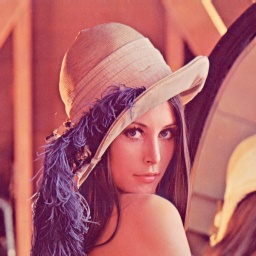
\includegraphics[height=6cm]{imagenes/lena_color_256.jpg}
	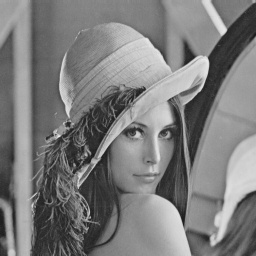
\includegraphics[height=6cm]{imagenes/lena_gray_256.jpg}
	\caption{Paso a escala de grises}
	\label{fig:grayscale_conversion}
\end{figure}

Asimismo se pueden aplicar con mayor facilidad modificaciones en el histograma. La principal de estas modificaciones aplicadas ha sido la normalización durante varios momentos de la obtención de características. Se procede a explicar aquí qué es la normalización, aunque realmente se aplica en pasos posteriores\cite{histogramEqualization}.

La normalización, ecualización o estiramiento lineal del histograma consiste en ampliar la gama cromática empleada en una imagen hasta ajustarla al número máximo de colores de que puede disponer esta imagen. Supongamos que tenemos una imagen en escala de grises ${X}$ y supongamos que $n_{i} \in \mathbb{N}_{0,255}$ es el número de ocurrencias de un nivel de grises $i$. Tenemos que la probabilidad de que haya un pixel con valor i en la imagen es:
\[
	p_{x}(i) = p(x=i)=\frac{n-{i}}{n}, 0 \leq i < L
\]
Definimos una función de distribución acumulativa ($fda$) que coincide con el histograma normal ecualizado y que se relaciona con $p_{x}$ de la siguiente manera:
\[
	fda_{x}(i) = \sum_{j=0}^{i}p_{x}(j)
\]
El estiramiento lineal consistirá en la creación de una nueva imagen $y$ en la que se interpolarán los valores de $fda$ a lo largo de todo el espectro de valores disponibles $\mathbb{N}_{0,255}$. Esto lo conseguimos multiplicando por una constante K cada valor para que la función de distribución de la nueva imagen sea:
\[
	fda_{y}(i)=iK
\]
La función de distribución acumulativa tiene nos permite hacer su inversa, definida como:
\[
	y = T(x) = fda_{x}(x)
\]
Teniendo en cuenta que $T(x)$ nos devolvería los valores en un intervalo $\left[0..1\right]$ debemos interpolar los valores contra el rango $\mathbb{N}_{0,255}$:
\[
	y' = y' (\max{x} - \min {x}) + \min{x}
\]

\begin{figure}[h!]
	\centering
	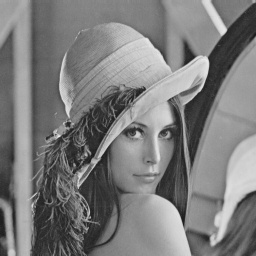
\includegraphics[height=6cm]{imagenes/lena_gray_256.jpg}
	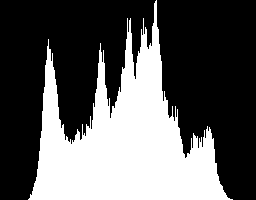
\includegraphics[width=6cm, height=2cm]{imagenes/lena_gray_256_hist.png}\\
	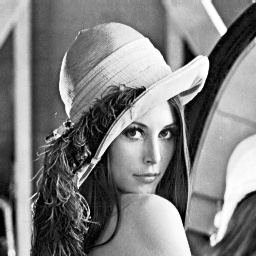
\includegraphics[height=6cm]{imagenes/lena_gray_256_equalized.jpg}
	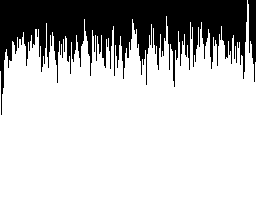
\includegraphics[width=6cm, height=2cm]{imagenes/lena_gray_256_equalized_hist.png}
	\caption{Normalización de histograma}
	\label{fig:normalize_hist}
\end{figure}

En la figura \ref{fig:normalize_hist} se muestran respectivamente una imagen en escala de grises junto a su histograma y en la siguiente línea, la misma imagen normalizada junto a su histograma, que podríamos considerar una representación gráfica de la $fda(x)$, donde cada punto en el eje X de la imagen se corresponde a un valor $i$ y en el eje Y vemos la aportación $p_{X}(i)$ que realiza a la imagen. se puede comprobar que:
\begin{itemize}
	\item{La imagen normalizada tiene un mayor rango de valores, con lo que aumenta el contraste entre las zonas oscuras y las zonas claras}
	\item{Como consecuencia de lo anterior, los bordes entre objetos quedan mejor demarcados.}
	\item{El histograma normalizado ocupa todo el rango $i$ de valores posibles. }
\end{itemize}

\newpage

\section{Determinación de la ubicación de la cara}
Para determinar las coordenadas en las que se encuentra la cara se utiliza el método mediante detección en cascada con identificadores de Haar \cite{ViolaJones}. Este es un algoritmo que requiere de un entrenamiento de imágenes en las que se haya identificado la forma que se desea extraer. Este entrenamiento genera un clasificador en cascada\footnote{Un buen clasificador en cascada se obtiene a partir de las 7000 imágenes. El clasificador empleado en este proyecto era el que venía por defecto con la librería Opencv.} gracias al cual después la búsqueda de los objetos con formas similares al solicitado es muy rápida. 
%Casi toda la teoría, con dibujitos, formulitas y SOBRETODO referencia al Viola-Jones
\begin{figure}[!hbt]
	\centering
	% Graphic for TeX using PGF
% Title: /home/bruno/pfc_UOC/PFM_UOC/memoria/diagramas/clasificadoresHaar.dia
% Creator: Dia v0.97
% CreationDate: Sun Jun  6 11:15:45 2010
% For: bruno
% \usepackage{tikz}
% The following commands are not supported in PSTricks at present
% We define them conditionally, so when they are implemented,
% this pgf file will use them.
\ifx\du\undefined
  \newlength{\du}
\fi
\setlength{\du}{15\unitlength}
\begin{tikzpicture}
\pgftransformxscale{1.000000}
\pgftransformyscale{-1.000000}
\definecolor{dialinecolor}{rgb}{0.000000, 0.000000, 0.000000}
\pgfsetstrokecolor{dialinecolor}
\definecolor{dialinecolor}{rgb}{1.000000, 1.000000, 1.000000}
\pgfsetfillcolor{dialinecolor}
\pgfsetlinewidth{0.100000\du}
\pgfsetdash{}{0pt}
\pgfsetdash{}{0pt}
\pgfsetmiterjoin
\definecolor{dialinecolor}{rgb}{0.000000, 0.000000, 0.000000}
\pgfsetstrokecolor{dialinecolor}
\draw (2.000000\du,2.000000\du)--(2.000000\du,8.000000\du)--(12.000000\du,8.000000\du)--(12.000000\du,2.000000\du)--cycle;
\pgfsetlinewidth{0.100000\du}
\pgfsetdash{}{0pt}
\pgfsetdash{}{0pt}
\pgfsetmiterjoin
\definecolor{dialinecolor}{rgb}{1.000000, 1.000000, 1.000000}
\pgfsetfillcolor{dialinecolor}
\fill (3.000000\du,3.000000\du)--(3.000000\du,7.000000\du)--(4.000000\du,7.000000\du)--(4.000000\du,3.000000\du)--cycle;
\definecolor{dialinecolor}{rgb}{0.000000, 0.000000, 0.000000}
\pgfsetstrokecolor{dialinecolor}
\draw (3.000000\du,3.000000\du)--(3.000000\du,7.000000\du)--(4.000000\du,7.000000\du)--(4.000000\du,3.000000\du)--cycle;
\pgfsetlinewidth{0.100000\du}
\pgfsetdash{}{0pt}
\pgfsetdash{}{0pt}
\pgfsetmiterjoin
\definecolor{dialinecolor}{rgb}{0.000000, 0.000000, 0.000000}
\pgfsetfillcolor{dialinecolor}
\fill (4.000000\du,3.000000\du)--(4.000000\du,7.000000\du)--(5.000000\du,7.000000\du)--(5.000000\du,3.000000\du)--cycle;
\definecolor{dialinecolor}{rgb}{0.000000, 0.000000, 0.000000}
\pgfsetstrokecolor{dialinecolor}
\draw (4.000000\du,3.000000\du)--(4.000000\du,7.000000\du)--(5.000000\du,7.000000\du)--(5.000000\du,3.000000\du)--cycle;
\pgfsetlinewidth{0.100000\du}
\pgfsetdash{}{0pt}
\pgfsetdash{}{0pt}
\pgfsetmiterjoin
\definecolor{dialinecolor}{rgb}{0.000000, 0.000000, 0.000000}
\pgfsetstrokecolor{dialinecolor}
\draw (13.000000\du,2.000000\du)--(13.000000\du,8.000000\du)--(23.000000\du,8.000000\du)--(23.000000\du,2.000000\du)--cycle;
\pgfsetlinewidth{0.100000\du}
\pgfsetdash{}{0pt}
\pgfsetdash{}{0pt}
\pgfsetmiterjoin
\definecolor{dialinecolor}{rgb}{1.000000, 1.000000, 1.000000}
\pgfsetfillcolor{dialinecolor}
\fill (14.000000\du,3.000000\du)--(14.000000\du,5.000000\du)--(16.000000\du,5.000000\du)--(16.000000\du,3.000000\du)--cycle;
\definecolor{dialinecolor}{rgb}{0.000000, 0.000000, 0.000000}
\pgfsetstrokecolor{dialinecolor}
\draw (14.000000\du,3.000000\du)--(14.000000\du,5.000000\du)--(16.000000\du,5.000000\du)--(16.000000\du,3.000000\du)--cycle;
\pgfsetlinewidth{0.100000\du}
\pgfsetdash{}{0pt}
\pgfsetdash{}{0pt}
\pgfsetmiterjoin
\definecolor{dialinecolor}{rgb}{0.000000, 0.000000, 0.000000}
\pgfsetfillcolor{dialinecolor}
\fill (14.000000\du,5.000000\du)--(14.000000\du,7.000000\du)--(16.000000\du,7.000000\du)--(16.000000\du,5.000000\du)--cycle;
\definecolor{dialinecolor}{rgb}{0.000000, 0.000000, 0.000000}
\pgfsetstrokecolor{dialinecolor}
\draw (14.000000\du,5.000000\du)--(14.000000\du,7.000000\du)--(16.000000\du,7.000000\du)--(16.000000\du,5.000000\du)--cycle;
\pgfsetlinewidth{0.100000\du}
\pgfsetdash{}{0pt}
\pgfsetdash{}{0pt}
\pgfsetmiterjoin
\definecolor{dialinecolor}{rgb}{0.000000, 0.000000, 0.000000}
\pgfsetstrokecolor{dialinecolor}
\draw (2.000000\du,10.000000\du)--(2.000000\du,16.000000\du)--(12.000000\du,16.000000\du)--(12.000000\du,10.000000\du)--cycle;
\pgfsetlinewidth{0.100000\du}
\pgfsetdash{}{0pt}
\pgfsetdash{}{0pt}
\pgfsetmiterjoin
\definecolor{dialinecolor}{rgb}{0.000000, 0.000000, 0.000000}
\pgfsetstrokecolor{dialinecolor}
\draw (13.000000\du,10.000000\du)--(13.000000\du,16.000000\du)--(23.000000\du,16.000000\du)--(23.000000\du,10.000000\du)--cycle;
\pgfsetlinewidth{0.100000\du}
\pgfsetdash{}{0pt}
\pgfsetdash{}{0pt}
\pgfsetmiterjoin
\definecolor{dialinecolor}{rgb}{1.000000, 1.000000, 1.000000}
\pgfsetfillcolor{dialinecolor}
\fill (14.000000\du,11.000000\du)--(14.000000\du,13.000000\du)--(15.000000\du,13.000000\du)--(15.000000\du,11.000000\du)--cycle;
\definecolor{dialinecolor}{rgb}{0.000000, 0.000000, 0.000000}
\pgfsetstrokecolor{dialinecolor}
\draw (14.000000\du,11.000000\du)--(14.000000\du,13.000000\du)--(15.000000\du,13.000000\du)--(15.000000\du,11.000000\du)--cycle;
\pgfsetlinewidth{0.100000\du}
\pgfsetdash{}{0pt}
\pgfsetdash{}{0pt}
\pgfsetmiterjoin
\definecolor{dialinecolor}{rgb}{0.000000, 0.000000, 0.000000}
\pgfsetfillcolor{dialinecolor}
\fill (14.000000\du,13.000000\du)--(14.000000\du,15.000000\du)--(15.000000\du,15.000000\du)--(15.000000\du,13.000000\du)--cycle;
\definecolor{dialinecolor}{rgb}{0.000000, 0.000000, 0.000000}
\pgfsetstrokecolor{dialinecolor}
\draw (14.000000\du,13.000000\du)--(14.000000\du,15.000000\du)--(15.000000\du,15.000000\du)--(15.000000\du,13.000000\du)--cycle;
\pgfsetlinewidth{0.100000\du}
\pgfsetdash{}{0pt}
\pgfsetdash{}{0pt}
\pgfsetmiterjoin
\definecolor{dialinecolor}{rgb}{1.000000, 1.000000, 1.000000}
\pgfsetfillcolor{dialinecolor}
\fill (3.000000\du,11.000000\du)--(3.000000\du,13.000000\du)--(5.000000\du,13.000000\du)--(5.000000\du,11.000000\du)--cycle;
\definecolor{dialinecolor}{rgb}{0.000000, 0.000000, 0.000000}
\pgfsetstrokecolor{dialinecolor}
\draw (3.000000\du,11.000000\du)--(3.000000\du,13.000000\du)--(5.000000\du,13.000000\du)--(5.000000\du,11.000000\du)--cycle;
\pgfsetlinewidth{0.100000\du}
\pgfsetdash{}{0pt}
\pgfsetdash{}{0pt}
\pgfsetmiterjoin
\definecolor{dialinecolor}{rgb}{1.000000, 1.000000, 1.000000}
\pgfsetfillcolor{dialinecolor}
\fill (7.000000\du,11.000000\du)--(7.000000\du,13.000000\du)--(9.000000\du,13.000000\du)--(9.000000\du,11.000000\du)--cycle;
\definecolor{dialinecolor}{rgb}{0.000000, 0.000000, 0.000000}
\pgfsetstrokecolor{dialinecolor}
\draw (7.000000\du,11.000000\du)--(7.000000\du,13.000000\du)--(9.000000\du,13.000000\du)--(9.000000\du,11.000000\du)--cycle;
\pgfsetlinewidth{0.100000\du}
\pgfsetdash{}{0pt}
\pgfsetdash{}{0pt}
\pgfsetmiterjoin
\definecolor{dialinecolor}{rgb}{0.000000, 0.000000, 0.000000}
\pgfsetfillcolor{dialinecolor}
\fill (5.000000\du,11.000000\du)--(5.000000\du,13.000000\du)--(7.000000\du,13.000000\du)--(7.000000\du,11.000000\du)--cycle;
\definecolor{dialinecolor}{rgb}{0.000000, 0.000000, 0.000000}
\pgfsetstrokecolor{dialinecolor}
\draw (5.000000\du,11.000000\du)--(5.000000\du,13.000000\du)--(7.000000\du,13.000000\du)--(7.000000\du,11.000000\du)--cycle;
\pgfsetlinewidth{0.100000\du}
\pgfsetdash{}{0pt}
\pgfsetdash{}{0pt}
\pgfsetmiterjoin
\definecolor{dialinecolor}{rgb}{0.000000, 0.000000, 0.000000}
\pgfsetfillcolor{dialinecolor}
\fill (15.000000\du,11.000000\du)--(15.000000\du,13.000000\du)--(16.000000\du,13.000000\du)--(16.000000\du,11.000000\du)--cycle;
\definecolor{dialinecolor}{rgb}{0.000000, 0.000000, 0.000000}
\pgfsetstrokecolor{dialinecolor}
\draw (15.000000\du,11.000000\du)--(15.000000\du,13.000000\du)--(16.000000\du,13.000000\du)--(16.000000\du,11.000000\du)--cycle;
\pgfsetlinewidth{0.100000\du}
\pgfsetdash{}{0pt}
\pgfsetdash{}{0pt}
\pgfsetmiterjoin
\definecolor{dialinecolor}{rgb}{1.000000, 1.000000, 1.000000}
\pgfsetfillcolor{dialinecolor}
\fill (15.000000\du,13.000000\du)--(15.000000\du,15.000000\du)--(16.000000\du,15.000000\du)--(16.000000\du,13.000000\du)--cycle;
\definecolor{dialinecolor}{rgb}{0.000000, 0.000000, 0.000000}
\pgfsetstrokecolor{dialinecolor}
\draw (15.000000\du,13.000000\du)--(15.000000\du,15.000000\du)--(16.000000\du,15.000000\du)--(16.000000\du,13.000000\du)--cycle;
% setfont left to latex
\definecolor{dialinecolor}{rgb}{0.000000, 0.000000, 0.000000}
\pgfsetstrokecolor{dialinecolor}
\node[anchor=west] at (7.000000\du,9.000000\du){A};
% setfont left to latex
\definecolor{dialinecolor}{rgb}{0.000000, 0.000000, 0.000000}
\pgfsetstrokecolor{dialinecolor}
\node[anchor=west] at (18.000000\du,9.000000\du){B};
% setfont left to latex
\definecolor{dialinecolor}{rgb}{0.000000, 0.000000, 0.000000}
\pgfsetstrokecolor{dialinecolor}
\node[anchor=west] at (7.000000\du,17.000000\du){C};
% setfont left to latex
\definecolor{dialinecolor}{rgb}{0.000000, 0.000000, 0.000000}
\pgfsetstrokecolor{dialinecolor}
\node[anchor=west] at (18.000000\du,17.000000\du){D};
\end{tikzpicture}

	\caption{Identificadores de Haar}
	\label{fig:Haar_identifiers}
\end{figure}

\begin{figure}[!hbt]
	\centering
	% Graphic for TeX using PGF
% Title: /home/bruno/pfc_UOC/PFM_UOC/memoria/diagramas/integralHaar.dia
% Creator: Dia v0.97
% CreationDate: Sun Jun  6 11:17:09 2010
% For: bruno
% \usepackage{tikz}
% The following commands are not supported in PSTricks at present
% We define them conditionally, so when they are implemented,
% this pgf file will use them.
\ifx\du\undefined
  \newlength{\du}
\fi
\setlength{\du}{15\unitlength}
\begin{tikzpicture}
\pgftransformxscale{1.000000}
\pgftransformyscale{-1.000000}
\definecolor{dialinecolor}{rgb}{0.000000, 0.000000, 0.000000}
\pgfsetstrokecolor{dialinecolor}
\definecolor{dialinecolor}{rgb}{1.000000, 1.000000, 1.000000}
\pgfsetfillcolor{dialinecolor}
\pgfsetlinewidth{0.100000\du}
\pgfsetdash{}{0pt}
\pgfsetdash{}{0pt}
\pgfsetmiterjoin
\definecolor{dialinecolor}{rgb}{1.000000, 1.000000, 1.000000}
\pgfsetfillcolor{dialinecolor}
\fill (1.000000\du,1.000000\du)--(1.000000\du,12.000000\du)--(18.850000\du,12.000000\du)--(18.850000\du,1.000000\du)--cycle;
\definecolor{dialinecolor}{rgb}{0.000000, 0.000000, 0.000000}
\pgfsetstrokecolor{dialinecolor}
\draw (1.000000\du,1.000000\du)--(1.000000\du,12.000000\du)--(18.850000\du,12.000000\du)--(18.850000\du,1.000000\du)--cycle;
\pgfsetlinewidth{0.100000\du}
\pgfsetdash{}{0pt}
\pgfsetdash{}{0pt}
\pgfsetmiterjoin
\definecolor{dialinecolor}{rgb}{0.000000, 0.000000, 0.000000}
\pgfsetfillcolor{dialinecolor}
\fill (1.000000\du,1.000000\du)--(1.000000\du,6.000000\du)--(7.000000\du,6.000000\du)--(7.000000\du,1.000000\du)--cycle;
\definecolor{dialinecolor}{rgb}{0.000000, 0.000000, 0.000000}
\pgfsetstrokecolor{dialinecolor}
\draw (1.000000\du,1.000000\du)--(1.000000\du,6.000000\du)--(7.000000\du,6.000000\du)--(7.000000\du,1.000000\du)--cycle;
% setfont left to latex
\definecolor{dialinecolor}{rgb}{0.000000, 0.000000, 0.000000}
\pgfsetstrokecolor{dialinecolor}
\node[anchor=west] at (8.000000\du,6.000000\du){(x,y)};
\end{tikzpicture}

	\caption{Integral de una imagen}
	\label{fig:image_integral}
\end{figure}

La base del funcionamiento del algoritmo es que en lugar de tratar con la imagen píxel a píxel, se trata con integrales de regiones de ella en regiones puntuales (que llamaremos clasificadores), como las que se pueden ver en la figura \ref{fig:Haar_identifiers}. Con estos clasificadores podríamos encontrar varios tipos de contorno en la imagen: con el clasificador A podríamos buscar bordes horizontales, con el B, bordes verticales, con el C líneas horizontales y con el D, líneas diagonales. Las integrales citadas son relativamente sencillas de comprender, dada una imagen $I$, la integral hasta la posición $(x,y)$ que se puede ver en la figura \ref{fig:image_integral} es la suma de los píxeles de esa región de la imagen. Formalmente:
\[ 
	iI(x,y) = \sum_{i,j=0}^{x,y}i(i,j)
\]
Donde $iI(x,y)$ es la integral de la imagen e $I(x,y)$ es la imagen original. Si se utilizan la recurrencias:
\[ 
	s(x,y)=s(x,y)-1 + I(x,y)
	iI(x,y)=iI(x-1,y)+s(x,y)
\]
Donde $s$ es un sumatorio de columnas acumulado, y tanto éste como $iI$ toman valor 0 cuando estamos fuera de los bordes de la imagen, la imagen integral se puee calcular de manera recursiva con un número mínimo de operaciones. La imagen integral no se calcula sobre la totalidad de una imagen completa, sino sobre ventanas (porciones) de ella cuadradas, en el caso del proyecto se ha decidido que el tamaño de la ventana sea de 50x50 píxeles. 

Para la búsqueda de un clasificador correcto para una determinada forma, hay que tener en cuenta que las integrales empleadas nos dan, para cada ventana, un número mucho mayor de subintegrales que de píxeles en la imagen. Para descartar las características no relevantes se ha empleado un sistema de aprendizaje ``AdaBoost''. Éste es un sistema de ``aprendizaje débil'' en el sentido de que para todos los posibles valores $v$ para un clasificador que obtiene, descarta de manera voraz los que no le resultan relevantes. Esto quizá no da el clasificador idóneo, pero teniendo en cuenta que el coste de cálculo del idóneo podría ser $O(2^{v})$, pero la aproximación a este suele ser bastante precisa. En el cuadro \ref{tab:face_detection_stats} se puede observar la eficacia de este método de selección de clasificadores.

\subsection{Escalado de la imagen}
Una vez se ha hallado la ubicación de la cara, se escala el tamaño de ésta para poder estandarizar parte de los procesos. El tamaño que se ha considerado más válido para trabajar es el de 128x128 píxeles, a 1 byte per píxel. En la gran mayoría de las imágenes de los juegos de prueba este tamaño es inferior al detectado, pero en caso de tener que ampliar la imagen se aplicaría un filtro bilinear por la relación calidad/tiempo de ampliación que suele tener.

Un filtro bilinear se encarga de escalar una imagen interpolando los cuatro píxeles más cercanos a la posición futura\cite{bilinearInterpolation}. En este caso, dado que estamos reduciendo la imagen, se puede considerar una adición de ruido despreciable. Dada la situación de la figura \ref{fig:interp_bilinear}, donde los píxeles los píxeles de la imagen original serían $P(1,1), P(1,2), P(2,1)$ y $P(2,2)$, $d$ la distancia en el eje $y$ del resultado interpolado al píxel original y $d'$ el análogo del anterior en el eje $x$, el valor de $P'(x,y)$ en la imagen interpolada se calcularía según la siguiente fórmula:

\[ P'(x,y) = P(1,1) (1-d) (1-d')+ P(1,2) d (1-d') + P(2,1) d (1-d') + P(2,2) d d'
\]

\begin{figure}[h!]
        \centering
        % Graphic for TeX using PGF
% Title: /home/bruno/pfc_UOC/PAC3/pac3/diagramas/interp_bilinear.dia
% Creator: Dia v0.97
% CreationDate: Tue Apr 27 10:45:23 2010
% For: bruno
% \usepackage{tikz}
% The following commands are not supported in PSTricks at present
% We define them conditionally, so when they are implemented,
% this pgf file will use them.
\ifx\du\undefined
  \newlength{\du}
\fi
\setlength{\du}{15\unitlength}
\begin{tikzpicture}
\pgftransformxscale{1.000000}
\pgftransformyscale{-1.000000}
\definecolor{dialinecolor}{rgb}{0.000000, 0.000000, 0.000000}
\pgfsetstrokecolor{dialinecolor}
\definecolor{dialinecolor}{rgb}{1.000000, 1.000000, 1.000000}
\pgfsetfillcolor{dialinecolor}
\pgfsetlinewidth{0.100000\du}
\pgfsetdash{}{0pt}
\pgfsetdash{}{0pt}
\pgfsetbuttcap
{
\definecolor{dialinecolor}{rgb}{0.000000, 0.000000, 0.000000}
\pgfsetfillcolor{dialinecolor}
% was here!!!
\definecolor{dialinecolor}{rgb}{0.000000, 0.000000, 0.000000}
\pgfsetstrokecolor{dialinecolor}
\draw (6.000000\du,4.000000\du)--(6.000000\du,14.000000\du);
}
\pgfsetlinewidth{0.100000\du}
\pgfsetdash{}{0pt}
\pgfsetdash{}{0pt}
\pgfsetbuttcap
{
\definecolor{dialinecolor}{rgb}{0.000000, 0.000000, 0.000000}
\pgfsetfillcolor{dialinecolor}
% was here!!!
\definecolor{dialinecolor}{rgb}{0.000000, 0.000000, 0.000000}
\pgfsetstrokecolor{dialinecolor}
\draw (6.000000\du,4.000000\du)--(16.000000\du,4.000000\du);
}
\pgfsetlinewidth{0.100000\du}
\pgfsetdash{}{0pt}
\pgfsetdash{}{0pt}
\pgfsetbuttcap
{
\definecolor{dialinecolor}{rgb}{0.000000, 0.000000, 0.000000}
\pgfsetfillcolor{dialinecolor}
% was here!!!
\definecolor{dialinecolor}{rgb}{0.000000, 0.000000, 0.000000}
\pgfsetstrokecolor{dialinecolor}
\draw (6.000000\du,9.000000\du)--(16.000000\du,9.000000\du);
}
\pgfsetlinewidth{0.100000\du}
\pgfsetdash{}{0pt}
\pgfsetdash{}{0pt}
\pgfsetbuttcap
{
\definecolor{dialinecolor}{rgb}{0.000000, 0.000000, 0.000000}
\pgfsetfillcolor{dialinecolor}
% was here!!!
\definecolor{dialinecolor}{rgb}{0.000000, 0.000000, 0.000000}
\pgfsetstrokecolor{dialinecolor}
\draw (6.000000\du,14.000000\du)--(16.000000\du,14.000000\du);
}
\pgfsetlinewidth{0.100000\du}
\pgfsetdash{}{0pt}
\pgfsetdash{}{0pt}
\pgfsetbuttcap
{
\definecolor{dialinecolor}{rgb}{0.000000, 0.000000, 0.000000}
\pgfsetfillcolor{dialinecolor}
% was here!!!
\definecolor{dialinecolor}{rgb}{0.000000, 0.000000, 0.000000}
\pgfsetstrokecolor{dialinecolor}
\draw (11.000000\du,4.000000\du)--(11.000000\du,14.000000\du);
}
\pgfsetlinewidth{0.100000\du}
\pgfsetdash{}{0pt}
\pgfsetdash{}{0pt}
\pgfsetbuttcap
{
\definecolor{dialinecolor}{rgb}{0.000000, 0.000000, 0.000000}
\pgfsetfillcolor{dialinecolor}
% was here!!!
\definecolor{dialinecolor}{rgb}{0.000000, 0.000000, 0.000000}
\pgfsetstrokecolor{dialinecolor}
\draw (16.000000\du,4.000000\du)--(16.000000\du,14.000000\du);
}
% setfont left to latex
\definecolor{dialinecolor}{rgb}{0.000000, 0.000000, 0.000000}
\pgfsetstrokecolor{dialinecolor}
\node[anchor=west] at (7.000000\du,6.000000\du){P(1,1)};
% setfont left to latex
\definecolor{dialinecolor}{rgb}{0.000000, 0.000000, 0.000000}
\pgfsetstrokecolor{dialinecolor}
\node[anchor=west] at (7.000000\du,13.000000\du){P(2,1)};
% setfont left to latex
\definecolor{dialinecolor}{rgb}{0.000000, 0.000000, 0.000000}
\pgfsetstrokecolor{dialinecolor}
\node[anchor=west] at (13.000000\du,6.000000\du){P(1,2)};
% setfont left to latex
\definecolor{dialinecolor}{rgb}{0.000000, 0.000000, 0.000000}
\pgfsetstrokecolor{dialinecolor}
\node[anchor=west] at (13.000000\du,13.000000\du){P(2,2)};
\pgfsetlinewidth{0.100000\du}
\pgfsetdash{{1.000000\du}{1.000000\du}}{0\du}
\pgfsetdash{{0.300000\du}{0.300000\du}}{0\du}
\pgfsetbuttcap
{
\definecolor{dialinecolor}{rgb}{0.000000, 0.000000, 0.000000}
\pgfsetfillcolor{dialinecolor}
% was here!!!
\definecolor{dialinecolor}{rgb}{0.000000, 0.000000, 0.000000}
\pgfsetstrokecolor{dialinecolor}
\draw (8.000000\du,12.000000\du)--(8.000000\du,7.000000\du);
}
\pgfsetlinewidth{0.100000\du}
\pgfsetdash{{0.300000\du}{0.300000\du}}{0\du}
\pgfsetdash{{0.300000\du}{0.300000\du}}{0\du}
\pgfsetbuttcap
{
\definecolor{dialinecolor}{rgb}{0.000000, 0.000000, 0.000000}
\pgfsetfillcolor{dialinecolor}
% was here!!!
\definecolor{dialinecolor}{rgb}{0.000000, 0.000000, 0.000000}
\pgfsetstrokecolor{dialinecolor}
\draw (14.000000\du,12.000000\du)--(14.000000\du,7.000000\du);
}
\pgfsetlinewidth{0.100000\du}
\pgfsetdash{{0.300000\du}{0.300000\du}}{0\du}
\pgfsetdash{{0.300000\du}{0.300000\du}}{0\du}
\pgfsetbuttcap
{
\definecolor{dialinecolor}{rgb}{0.000000, 0.000000, 0.000000}
\pgfsetfillcolor{dialinecolor}
% was here!!!
\definecolor{dialinecolor}{rgb}{0.000000, 0.000000, 0.000000}
\pgfsetstrokecolor{dialinecolor}
\draw (14.000000\du,7.000000\du)--(8.000000\du,7.000000\du);
}
\pgfsetlinewidth{0.100000\du}
\pgfsetdash{}{0pt}
\pgfsetdash{}{0pt}
\pgfsetbuttcap
{
\definecolor{dialinecolor}{rgb}{0.000000, 0.000000, 0.000000}
\pgfsetfillcolor{dialinecolor}
% was here!!!
\pgfsetarrowsend{stealth}
\definecolor{dialinecolor}{rgb}{0.000000, 0.000000, 0.000000}
\pgfsetstrokecolor{dialinecolor}
\draw (10.000000\du,11.000000\du)--(31.000000\du,7.000000\du);
}
\definecolor{dialinecolor}{rgb}{0.000000, 0.000000, 0.000000}
\pgfsetstrokecolor{dialinecolor}
\draw (10.000000\du,11.000000\du)--(31.000000\du,7.000000\du);
\pgfsetlinewidth{0.100000\du}
\pgfsetdash{}{0pt}
\pgfsetmiterjoin
\pgfsetbuttcap
\definecolor{dialinecolor}{rgb}{0.000000, 0.000000, 0.000000}
\pgfsetfillcolor{dialinecolor}
\pgfpathmoveto{\pgfpoint{10.000000\du}{11.000000\du}}
\pgfpathcurveto{\pgfpoint{9.976611\du}{10.877208\du}}{\pgfpoint{10.076014\du}{10.731026\du}}{\pgfpoint{10.198807\du}{10.707637\du}}
\pgfpathcurveto{\pgfpoint{10.321599\du}{10.684248\du}}{\pgfpoint{10.467780\du}{10.783652\du}}{\pgfpoint{10.491169\du}{10.906444\du}}
\pgfpathcurveto{\pgfpoint{10.514558\du}{11.029236\du}}{\pgfpoint{10.415155\du}{11.175418\du}}{\pgfpoint{10.292363\du}{11.198807\du}}
\pgfpathcurveto{\pgfpoint{10.169570\du}{11.222196\du}}{\pgfpoint{10.023389\du}{11.122792\du}}{\pgfpoint{10.000000\du}{11.000000\du}}
\pgfusepath{fill}
\definecolor{dialinecolor}{rgb}{0.000000, 0.000000, 0.000000}
\pgfsetstrokecolor{dialinecolor}
\pgfpathmoveto{\pgfpoint{10.000000\du}{11.000000\du}}
\pgfpathcurveto{\pgfpoint{9.976611\du}{10.877208\du}}{\pgfpoint{10.076014\du}{10.731026\du}}{\pgfpoint{10.198807\du}{10.707637\du}}
\pgfpathcurveto{\pgfpoint{10.321599\du}{10.684248\du}}{\pgfpoint{10.467780\du}{10.783652\du}}{\pgfpoint{10.491169\du}{10.906444\du}}
\pgfpathcurveto{\pgfpoint{10.514558\du}{11.029236\du}}{\pgfpoint{10.415155\du}{11.175418\du}}{\pgfpoint{10.292363\du}{11.198807\du}}
\pgfpathcurveto{\pgfpoint{10.169570\du}{11.222196\du}}{\pgfpoint{10.023389\du}{11.122792\du}}{\pgfpoint{10.000000\du}{11.000000\du}}
\pgfusepath{stroke}
\pgfsetlinewidth{0.100000\du}
\pgfsetdash{{\pgflinewidth}{0.200000\du}}{0cm}
\pgfsetdash{{\pgflinewidth}{0.200000\du}}{0cm}
\pgfsetbuttcap
{
\definecolor{dialinecolor}{rgb}{0.000000, 0.000000, 0.000000}
\pgfsetfillcolor{dialinecolor}
% was here!!!
\definecolor{dialinecolor}{rgb}{0.000000, 0.000000, 0.000000}
\pgfsetstrokecolor{dialinecolor}
\draw (8.000000\du,11.000000\du)--(10.000000\du,11.000000\du);
}
\pgfsetlinewidth{0.100000\du}
\pgfsetdash{{\pgflinewidth}{0.200000\du}}{0cm}
\pgfsetdash{{\pgflinewidth}{0.200000\du}}{0cm}
\pgfsetbuttcap
{
\definecolor{dialinecolor}{rgb}{0.000000, 0.000000, 0.000000}
\pgfsetfillcolor{dialinecolor}
% was here!!!
\definecolor{dialinecolor}{rgb}{0.000000, 0.000000, 0.000000}
\pgfsetstrokecolor{dialinecolor}
\draw (10.000000\du,11.000000\du)--(10.000000\du,7.000000\du);
}
% setfont left to latex
\definecolor{dialinecolor}{rgb}{0.000000, 0.000000, 0.000000}
\pgfsetstrokecolor{dialinecolor}
\node[anchor=west] at (10.000000\du,8.000000\du){d'};
% setfont left to latex
\definecolor{dialinecolor}{rgb}{0.000000, 0.000000, 0.000000}
\pgfsetstrokecolor{dialinecolor}
\node[anchor=west] at (9.000000\du,12.000000\du){d};
\pgfsetlinewidth{0.100000\du}
\pgfsetdash{}{0pt}
\pgfsetdash{}{0pt}
\pgfsetbuttcap
{
\definecolor{dialinecolor}{rgb}{0.000000, 0.000000, 0.000000}
\pgfsetfillcolor{dialinecolor}
% was here!!!
\definecolor{dialinecolor}{rgb}{0.000000, 0.000000, 0.000000}
\pgfsetstrokecolor{dialinecolor}
\draw (23.000000\du,3.000000\du)--(23.000000\du,15.000000\du);
}
\pgfsetlinewidth{0.100000\du}
\pgfsetdash{}{0pt}
\pgfsetdash{}{0pt}
\pgfsetbuttcap
{
\definecolor{dialinecolor}{rgb}{0.000000, 0.000000, 0.000000}
\pgfsetfillcolor{dialinecolor}
% was here!!!
\definecolor{dialinecolor}{rgb}{0.000000, 0.000000, 0.000000}
\pgfsetstrokecolor{dialinecolor}
\draw (23.000000\du,3.000000\du)--(35.000000\du,3.000000\du);
}
\pgfsetlinewidth{0.100000\du}
\pgfsetdash{}{0pt}
\pgfsetdash{}{0pt}
\pgfsetbuttcap
{
\definecolor{dialinecolor}{rgb}{0.000000, 0.000000, 0.000000}
\pgfsetfillcolor{dialinecolor}
% was here!!!
\definecolor{dialinecolor}{rgb}{0.000000, 0.000000, 0.000000}
\pgfsetstrokecolor{dialinecolor}
\draw (23.000000\du,12.000000\du)--(35.000000\du,12.000000\du);
}
\pgfsetlinewidth{0.100000\du}
\pgfsetdash{}{0pt}
\pgfsetdash{}{0pt}
\pgfsetbuttcap
{
\definecolor{dialinecolor}{rgb}{0.000000, 0.000000, 0.000000}
\pgfsetfillcolor{dialinecolor}
% was here!!!
\definecolor{dialinecolor}{rgb}{0.000000, 0.000000, 0.000000}
\pgfsetstrokecolor{dialinecolor}
\draw (29.000000\du,3.000000\du)--(29.000000\du,15.000000\du);
}
\pgfsetlinewidth{0.100000\du}
\pgfsetdash{}{0pt}
\pgfsetdash{}{0pt}
\pgfsetbuttcap
{
\definecolor{dialinecolor}{rgb}{0.000000, 0.000000, 0.000000}
\pgfsetfillcolor{dialinecolor}
% was here!!!
\definecolor{dialinecolor}{rgb}{0.000000, 0.000000, 0.000000}
\pgfsetstrokecolor{dialinecolor}
\draw (26.000000\du,3.000000\du)--(26.000000\du,15.000000\du);
}
\pgfsetlinewidth{0.100000\du}
\pgfsetdash{}{0pt}
\pgfsetdash{}{0pt}
\pgfsetbuttcap
{
\definecolor{dialinecolor}{rgb}{0.000000, 0.000000, 0.000000}
\pgfsetfillcolor{dialinecolor}
% was here!!!
\definecolor{dialinecolor}{rgb}{0.000000, 0.000000, 0.000000}
\pgfsetstrokecolor{dialinecolor}
\draw (23.000000\du,9.000000\du)--(35.000000\du,9.000000\du);
}
\pgfsetlinewidth{0.100000\du}
\pgfsetdash{}{0pt}
\pgfsetdash{}{0pt}
\pgfsetbuttcap
{
\definecolor{dialinecolor}{rgb}{0.000000, 0.000000, 0.000000}
\pgfsetfillcolor{dialinecolor}
% was here!!!
\definecolor{dialinecolor}{rgb}{0.000000, 0.000000, 0.000000}
\pgfsetstrokecolor{dialinecolor}
\draw (32.000000\du,3.000000\du)--(32.000000\du,15.000000\du);
}
\pgfsetlinewidth{0.100000\du}
\pgfsetdash{}{0pt}
\pgfsetdash{}{0pt}
\pgfsetbuttcap
{
\definecolor{dialinecolor}{rgb}{0.000000, 0.000000, 0.000000}
\pgfsetfillcolor{dialinecolor}
% was here!!!
\definecolor{dialinecolor}{rgb}{0.000000, 0.000000, 0.000000}
\pgfsetstrokecolor{dialinecolor}
\draw (35.000000\du,3.000000\du)--(35.000000\du,15.000000\du);
}
\pgfsetlinewidth{0.100000\du}
\pgfsetdash{}{0pt}
\pgfsetdash{}{0pt}
\pgfsetbuttcap
{
\definecolor{dialinecolor}{rgb}{0.000000, 0.000000, 0.000000}
\pgfsetfillcolor{dialinecolor}
% was here!!!
\definecolor{dialinecolor}{rgb}{0.000000, 0.000000, 0.000000}
\pgfsetstrokecolor{dialinecolor}
\draw (23.000000\du,6.000000\du)--(35.000000\du,6.000000\du);
}
\pgfsetlinewidth{0.100000\du}
\pgfsetdash{}{0pt}
\pgfsetdash{}{0pt}
\pgfsetbuttcap
{
\definecolor{dialinecolor}{rgb}{0.000000, 0.000000, 0.000000}
\pgfsetfillcolor{dialinecolor}
% was here!!!
\definecolor{dialinecolor}{rgb}{0.000000, 0.000000, 0.000000}
\pgfsetstrokecolor{dialinecolor}
\draw (23.000000\du,15.000000\du)--(35.000000\du,15.000000\du);
}
% setfont left to latex
\definecolor{dialinecolor}{rgb}{0.000000, 0.000000, 0.000000}
\pgfsetstrokecolor{dialinecolor}
\node[anchor=west] at (31.000000\du,7.000000\du){P'};
\end{tikzpicture}

        \caption{Esquema de interpolación bilinear}
	\label{fig:interp_bilinear}
\end{figure}

Tras este paso, por consiguiente, habremos reducido el tamaño de trabajo a una matriz de 128x128 bytes. Escrito de manera formal, tendríamos que la imagen M se corresponde con la siguiente matriz:

\[ M=\left( \begin{array}{lcccccr} 
	m_{0,0} & m_{0,1} & m_{0,2} & \hdots & m_{0,125} & m_{0,126} & m_{0,127}\\
	m_{1,0} & m_{1,1} & m_{1,2} & \hdots & m_{1,125} & m_{1,126} & m_{1,127}\\
	\vdots & \vdots & \vdots & \ddots & \vdots & \vdots & \vdots \\
	m_{126,0} & m_{126,1} & m_{126,2} & \hdots & m_{126,125} & m_{126,126} & m_{126,127}\\
	m_{127,0} & m_{127,1} & m_{127,2} & \hdots & m_{127,125} & m_{127,126} & m_{127,127}
	\end{array} \right)
\]

%\[ \forall  m_{i,j} \in \mathbb{N} \and i_{i,j} \in \left[ 0..255 \right] \]
Donde $ \forall m_{i,j} \mid m_{i,j} \in \mathbb{N}_{\left[ 0,255 \right]} \wedge i,j \in \mathbb{N}_{\left[ 0,127 \right]} $
	

\subsection{Ubicación de los rasgos faciales}
Una vez disponemos de la cara ya escalada en BN, se llevan a cabo dos procesos:
\begin{itemize}
	\item{Localización de bordes aplicando el detector Sobel únicamente en orientación vertical}
	\item{Sobre el resultado previo aplicamos un algoritmo de ventana para hallar la ubicación de los ojos, la nariz y la boca.}
\end{itemize}

El detector de esquinas Sobel es muy conocido en el procesado de imagen\cite{opencv} y es relativamente rápido\footnote{Gracias a las mejoras del hardware actual (mayores anchos de banda de memoria, extensiones para el cálculo vectorial, cachés mayores, varios núcleos para paralelizar procesos...) la velocidad del procesado de imágenes ha mejorado exponencialmente. }. Informalmente, el Sobel halla los bordes de la imagen calculando una aproximación a la derivada de ésta, donde los máximos son el lugar donde hay un cambio en la imagen. En este proyecto utilizamos la convolución de la imagen con el siguiente kernel (informalmente, superponemos cada punto de la imagen con la siguiente matriz):

\[ \frac{\partial^{2}{M}}{\partial{y^{2}}} \approx S_{y}''= \left( \begin{array}{ccc} 1 & 2 & 1 \\ -2 & -4 & -2 \\ 1 & 2 & 1  \end{array} \right) \oplus M \]

Donde $\oplus$ es el operador de convolución. Concretamente, este es un kernel de apertura 3 (tamaño 3x3), para el cálculo de la segunda derivada en el eje Y. Nótese que en el proyecto únicamente se ha utilizado el kernel para calcular la derivada vertical, dado que con él hemos obtenido mejores resultados que calculando la derivada en ambos ejes\footnote{Como comentario, el kernel con el que debería de convolucionarse la imagen para el cálculo de la segunda derivada horizontal sería el resultante de la trasposición del kernel aquí aplicado.}.

Añadir que dado que el kernel es separable (existen $M$ y $N$ tales que $MN=S$) para optimizar el número de operaciones se puede realizar la convolución según la siguiente operación:

\[G_{x}=\left[ \begin{array}{c} 1 \\ -2 \\1 \end{array} \right] \oplus \left( \left[ \begin{array}{ccc} 1 & 2 & 1 \end{array}\right] \oplus M \right) \]

\begin{figure}[h!]
	\centering
	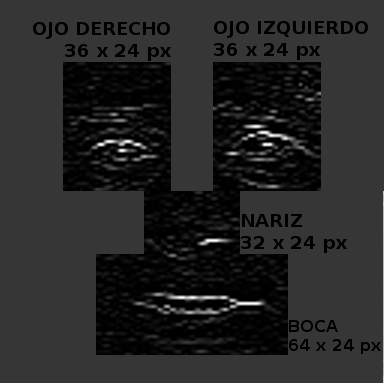
\includegraphics[width=8cm]{zonas_busqueda_cara.png}
	\caption{Máscara aplicada sobre la imagen y tamaños de ventana}
	\label{fig:imagen_mascaras}
\end{figure}

Tras la detección de esquinas, procedemos a la búsqueda de los ojos, nariz y boca. Para ello, buscamos en el resultante de aplicar la máscara de la figura \ref{fig:imagen_mascaras} un algoritmo para buscar la ventana del tamaño indicado con suma de mayor valor. La búsqueda se realiza en el eje vertical de la imagen. Informalmente, buscamos la ventana de tamaño WxH (indicados en la imagen) cuyo valor de sumatorio sea el máximo. Formalmente, la región K es la resultante de la máscara que aparece en la imagen y se expresaría de la siguiente manera:
\[
 K = \left( 
	\begin{array}{lcccr} 
		k_{0,0} & k_{0,1} & \hdots & k_{0,j-2} & k_{0,j-1} \\
		\vdots & \vdots & \ddots & \vdots & \vdots \\
		k_{i-1,0} & k_{i-1,1} & \hdots & k_{i-1,j-2} & k_{i-1,j-1} \\
	\end{array} \right)
\]
Y que buscamos el valor de m según la siguiente ecuación. El sumatorio de la submatriz [(0,m), (W,m+H)] tendrá el valor máximo de la máscara indicada.
\[
   V = K\left[\left(0,m\right), \left(W,m+H\right) \right] \mid \forall n \sum_{i=0,j=n}^{i=W,j=n+H} K_{i,j} \leq \sum_{p=0,q=m}^{p=W,q=m+H} K_{p,q} 
\]
Este método se ha mostrado fiable, rápido y paralelizable (búsqueda de ambos ojos y nariz como tres hilos de ejecución diferentes, y tras el resultado de la detección de la nariz se puede realizar la búsqueda de la boca) aunque se ha reconocido casos en los que puede dar problemas. En la figura \ref{fig:imagenes_procesadas} podemos observar:
\begin{itemize}
	\item{A la izquierda la imagen original en color, con la región en la que se ha detectado la cara encuadrada.}
	\item{A la derecha, la primera imagen desde arriba es la cara detectada tras aplicar la conversión a escala de grises y el redimensionado bilinear.}
	\item{Bajo la anterior, está la imagen resultante de la aplicación del detector de esquinas Sobel de segundo orden sobre el eje Y.}
	\item{Por debajo de la anterior, tenemos encuadradas las máximas ventanas según los criterios previamente señalados.}
	\item{Finalmente, la imagen inferior de la derecha es el resultado de aplicar las ventanas halladas sobre la cara en escala de grises y redimensionada}
\end{itemize}
\begin{figure}[h!]
	\centering
	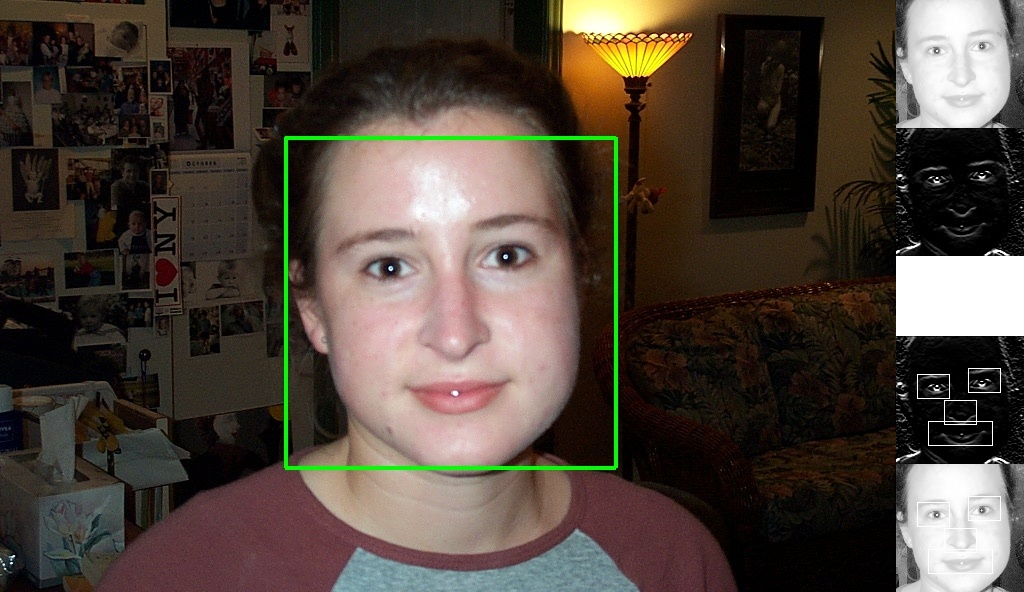
\includegraphics[width=12cm]{ejemplo_imagen_mujer.jpg}
	\caption{Pasos del procesado de la imagen}
	\label{fig:imagenes_procesadas}
\end{figure}
%si esto cuela y lo explico bien, doy volteretas

\newpage

\section{Extracción de características}
En estos momentos hemos determinado la región de interés a partir de la cual extraeremos la face signature. 
\subsection{Filtros de Gabor}
La transormada de Gabor es un caso especial de la transformada en tiempo discreto de Fourier. La función a transformar primero se convoluciona con una Gaussiana (se puede tratar como una ventana) y al resultado se le realiza una transformada de Fourier. En el caso monodimensional se definiría como:\\
\[
	G_{x}(t,f)=\int_{-\infty}^{+\infty}{e^{-\pi(\tau-t)^ 2e^{-2\pi jf \tau}}x(\tau)d\tau}
\]
	Debido a que la Gaussiana es una función definida entre $-\infty$ y $+\infty$ se debe asumir un comportamiento finito de ésta para que sea práctica y realizable. Si consideramos que la gaussiana :
\[
f(n) =  
\begin{cases}
	e^{-\pi a^2}\geq 10^{-5} & \parallel a \parallel \leq 1.9143 \\
	e^{-\pi a^2} < 10^{-5} & \parallel a \parallel > 1.9143 \\
\end{cases}
\]
Léase, que a partir de 1,9143 consideramos la contribución despreciable porque es inferior a $10^{-5}$. Haciendo esa aproximación nos queda la siguiente definición:
\[
	G_{x}(t,f)=\int_{-1.9143}^{+1.9143}{e^{-\pi(\tau-t)^ 2e^{-2\pi jf \tau}}x(\tau)d\tau}
\]
Dicha transformada tiene las siguientes propiedades: invertibilidad, linearidad, desplazamiento, modulación, propiedad de integración de potencia, propiedad de suma de energía, propiedad de reducción de propiedad, integrabilidad y recuperabilidad.\\
Un filtro de Gabor \cite{Lee96imagerepresentation} se podría considerar la aplicación de lo citado previamente al mundo de las señales discretas. Es un filtro lineal empleado en el procesado de imágenes para la detección de esquinas y características. Esta serie de filtros tienen un comportamiento frecuencial y de orientación similar al del córtex visual humano\cite{DaugmanCortexReceptors} y se consideran particularmente apropiados para representar y discriminar texturas. En el dominio espacial (2 dimensiones) el filtrado de la señal se realiza convolucionándola con el/los correspondiente/s kernel de Gabor. Los kernels de Gabor son una Gaussiana modulada con un plano senoidal\cite{DaugmanGaborTransforms}, y serían calculados con la siguiente fórmula:
\[
g(x,y;\lambda,\theta,\psi,\sigma,\gamma)=e^{-\frac{x'^2+\gamma^2y'^2}{2\sigma^2}}\cos\left(2\pi\frac{x'}{\lambda}+\psi\right)
\]

En esta expresión tenemos las siguientes variables:
\begin{itemize}
	\item{$\lambda$ es la longitud de onda del factor coseno}
	\item{$\phi$ es la orientación de la normal hacia las bandas paralelas de la función de Gabor\footnote{La función de Gabor ($g_{l,n}(x)=g(x-al)e^{2\pi ibnx}, -\infty < l,n < \infty, g\in L^2(R), \parallel g \parallel=1$ , donde $a$ y $b$ son constantes) fue desarrollada en 1946 por Dennis Gabor y se intentó aplicar para generar sonidos (sin éxito debido a que no tenía en cuenta el análisis frecuencial con respecto al tiempo de las señales de sonido en la vida real). No obstante, sentó precedente para la compresión de sonido y de vídeo. Se puede considerar una predecesora de las Wavelets. } }
	\item{$\psi$ es el desfase (orientación del kernel) }
	\item{$\sigma$ es la desviación estándar de la gaussiana convolucionada}
	\item{$\gamma$ es la ratio de aspecto espacial, que especifica la elipticidad de la función de Gabor con la que convolucionamos la gaussiana anterior.}
	\item{Los valores $ x'$ e $y'$ que son cambios de variable para los siguientes valores:} 
		\[ x' =x\cos\theta + y\sin\theta \] 
		\[y'=-x\sin\theta + y\cos\theta \] 
\end{itemize}

En la figura \ref{fig:gabor_example} tenemos un ejemplo del paso de una imagen sobre un banco de filtros de Gabor. La imagen original ocupa el primer tercio de la imagen y se ha elegido expresamente para comprobar la respuesta al filtro. El segundo tercio de la imagen contiene la representación de los kernel que se han empleado para convolucionar la imagen. Están agrupadas verticalmente por las orientaciones $\psi$ (0, 45, 90 y 135º respectivamente), mientras que horizontalmente están agrupadas por la desviación estándar de la gaussiana $\sigma$ (valores 16, 32, 64 y 128). En el tercio inferior se ve el resultado\footnote{Las imágenes han sido escaladas, se tiene que tener en cuenta que cada uno de los resultados tiene el mismo tamaño que la imagen original} de convolucionar la imagen original con cada uno de los kernels. Por ejemplo, cuando aplicamos el kernel con $\psi=0$ en el resultado no vemos la franja horizontal.

\begin{figure}[h!]
        \centering
	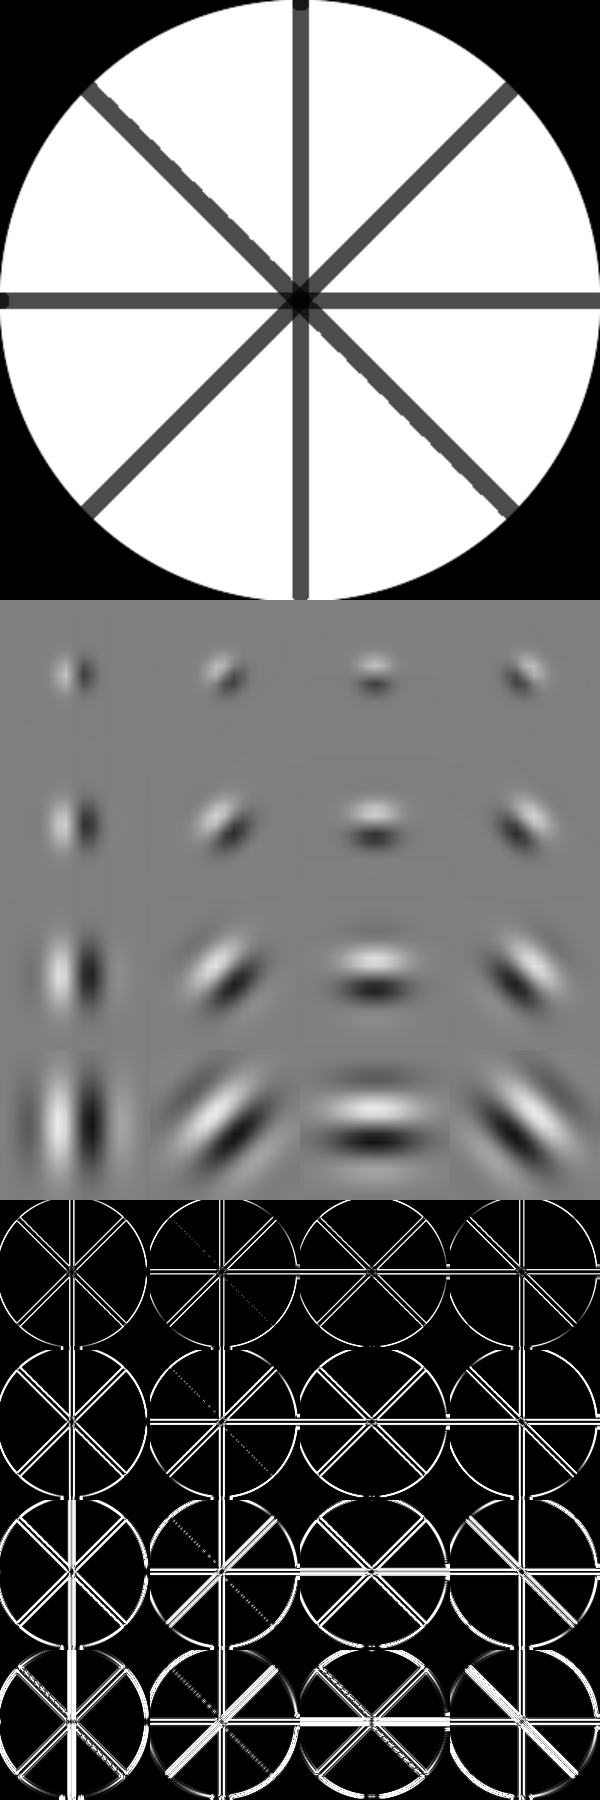
\includegraphics[height=21cm]{imagenes/Gabor.png}
        \caption{Aplicación de un banco de filtros de Gabor}
	\label{fig:gabor_example}
\end{figure}

\subsection{Obtención de la huella facial}
Para la obtención de la huella facial se han filtrado los rasgos (ojo derecho, ojo izquierdo, nariz y boca) por un filtro de Gabor. Dependiendo del uso que se le ha dado a la información obtenida tras el filtrado se han tenido en cuenta dos tipos de representación diferentes para la huella facial, las ventajas e inconvenientes de las cuales se detallarán posteriormente.

\begin{itemize}
	\item{Disposición lateral, en la que el resultado del filtrado por cada orientación se ha concatenado}
	\item{Superposición, en la que se ha hecho una suma ponderada de todos los resultados del filtrado por cada orientación}
\end{itemize}

Asímismo, también se ha umbralizado y aplicado el suavizado sobre las huellas faciales para comprobar si estadísticamente existía alguna mejora. También se detalla posteriormente.

\subsubsection{Disposición lateral de filtrados}
La disposición lateral de es una representación en la que se concatena en el eje X de la imagen cada uno de los resultados de convolucionar la imagen por cada uno de los filtros que forman parte del banco empleado. Las ventajas de este método de almacenamiento de la huella facial son las siguientes:
\begin{itemize}
	\item{Mejor respuesta estadística: da mejores resultados cuando se calcula la distancia entre dos face signatures}
	\item{Mejor visibilidad de cada una de las componentes empleadas}
\end{itemize}
A su vez, también tiene los siguientes inconvenientes:
\begin{itemize}
	\item{Tamaño de signature dependiente del tamaño del banco de filtros}
	\item{Mayor ocupación de memoria y de espacio en la base de datos}
	\item{Tiempos superiores para el cálculo de distancia entre individuos}
	\item{En caso de cambio del banco de filtros, se deben recrear todas las huellas faciales, toda la base de datos, etc.}
\end{itemize}
En la figura \ref{fig:filter_concat} podemos observar el funcionamiento de la concatenación de filtros. En la primera línea tenemos los rasgos obtenidos (ojo derecho, ojo izquierdo, nariz y boca). En las filas subsiguientes están el resultado de concatenar el filtrado de dichos rasgos en ese orden. Cada grupo de tres tiene las orientaciones $\psi = \alpha \in \left[0º,180º\right] | \alpha \mod{45º}=0$ ,  $\psi = \alpha \in \left[0º,180º\right] | \alpha \mod{20º}=0$,  $\psi = \alpha \in \left[0º,180º\right] | \alpha \mod{10º}=0$ respectivamente. Nótese que las imágenes están escaladas (todas tienen la misma altura en realidad), de tal manera que en verdad a cada orientación que se añade se estaría incrementando el tamaño de la huella facial.

\begin{figure}[h!]
	\centering
	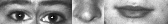
\includegraphics[width=15cm]{imagenes/M2_concat.jpg}\\

	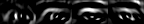
\includegraphics[width=15cm]{imagenes/M2_concat_od_45deg.png}
	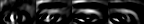
\includegraphics[width=15cm]{imagenes/M2_concat_oi_45deg.png}
	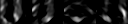
\includegraphics[width=15cm]{imagenes/M2_concat_nariz_45deg.png}
	
\includegraphics[width=15cm]{imagenes/M2_concat_boca_45deg.png}\\

	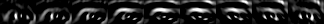
\includegraphics[width=15cm]{imagenes/M2_concat_od_20deg.png}
	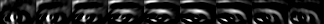
\includegraphics[width=15cm]{imagenes/M2_concat_oi_20deg.png}
	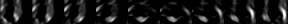
\includegraphics[width=15cm]{imagenes/M2_concat_nariz_20deg.png}
	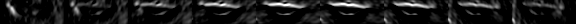
\includegraphics[width=15cm]{imagenes/M2_concat_boca_20deg.png}\\

	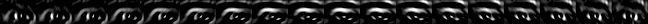
\includegraphics[width=15cm]{imagenes/M2_concat_od_10deg.png}
	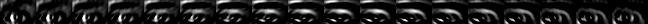
\includegraphics[width=15cm]{imagenes/M2_concat_oi_10deg.png}
	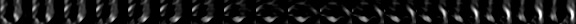
\includegraphics[width=15cm]{imagenes/M2_concat_nariz_10deg.png}
	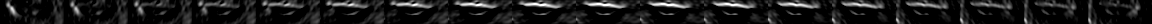
\includegraphics[width=15cm]{imagenes/M2_concat_boca_10deg.png}
	\caption{Concatenación de filtrados}
	\label{fig:filter_concat}
\end{figure}

\subsubsection{Superposición de filtrados}
En la superposición de filtrados, ponderamos el resultado de filtrar la imagen por cada uno de los filtros que forman parte del banco y los superponemos todos ellos sobre la imagen. Las ventajas principales de este método de almacenamiento de la huella facial son las siguientes:
\begin{itemize}
	\item{Tamaño de la signature constante, y de hecho es el mismo que el de la imagen filtrada}
	\item{Mejores tiempos en cálculo de distancias}
	\item{Menor espacio en memoria y en base de datos}
	\item{En caso de cambio del banco de filtros, puede mantenerse la misma huella facial, aunque las distancias puedan variar significativamente}
\end{itemize}
A su vez, también tiene los siguientes inconvenientes:
\begin{itemize}
	\item{Peor rendimiento estadístico: da más errores en los cálculos de distancia}
	\item{Se pierde la capacidad de determinar qué filtro es el que aporta más información a la face signature}
\end{itemize}

En la figura \ref{fig:filter_superp} podemos observar el funcionamiento de la superposición de filtros. En la primera línea tenemos los rasgos obtenidos (ojo derecho, ojo izquierdo, nariz y boca). En las filas subsiguientes están el resultado de superponer el filtrado de dichos rasgos en ese orden, y con $\psi = \alpha \in \left[0º,180º\right] | \alpha \mod{45º}=0$ ,  $\psi = \alpha \in \left[0º,180º\right] | \alpha \mod{20º}=0$,  $\psi = \alpha \in \left[0º,180º\right] | \alpha \mod{10º}=0$ respectivamente.

\begin{figure}[h!]
	\centering
	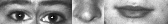
\includegraphics[width=15cm]{imagenes/M2_concat.jpg}\\
	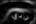
\includegraphics[width=3.6cm]{imagenes/M2_superpos_od_45deg.png}
	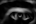
\includegraphics[width=3.6cm]{imagenes/M2_superpos_od_20deg.png}
	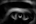
\includegraphics[width=3.6cm]{imagenes/M2_superpos_od_10deg.png}\\
	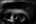
\includegraphics[width=3.6cm]{imagenes/M2_superpos_oi_45deg.png}
	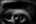
\includegraphics[width=3.6cm]{imagenes/M2_superpos_oi_20deg.png}
	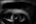
\includegraphics[width=3.6cm]{imagenes/M2_superpos_oi_10deg.png}\\
	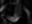
\includegraphics[width=3.2cm]{imagenes/M2_superpos_nariz_45deg.png}
	
\includegraphics[width=3.2cm]{imagenes/M2_superpos_nariz_20deg.png}
	
\includegraphics[width=3.2cm]{imagenes/M2_superpos_nariz_10deg.png}\\
	
\includegraphics[width=4cm]{imagenes/M2_superpos_boca_45deg.png}
	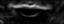
\includegraphics[width=4cm]{imagenes/M2_superpos_boca_20deg.png}
	
\includegraphics[width=4cm]{imagenes/M2_superpos_boca_10deg.png}
	\caption{Superposición de filtrados}
	\label{fig:filter_superp}
\end{figure}


\subsubsection{Umbralización}
La umbralización de una imagen $I$ es un proceso en el que a los píxeles que superan (o están por debajo) de un valor determinado $T$ se les aplica una modificación de valor. Durante la ejecución del proyecto se han probado tres tipos de umbralización: binarización, truncado y reducción a cero\footnote{La librería OpenCV permitía varios tipos más de umbralización.}.
\begin{itemize}
	\item{En la binarización a la imagen y al valor umbral (\textit{threshold} en inglés, de ahí el uso de T), se le añade como parámetro el valor M (de máximo) que es el que tomarán los píxeles que sobrepasen el umbral. Se puede ver un ejemplo en la imagen \ref{fig:thr_binarization}, en el que el valor máximo $M=255$ y el valor umbral es $T=(0,30,60,90)$ en la primera fila y $T=(120,150,180,210)$ en la segunda. Formalmente la binarización se define como:}
	\[
		thr(I,T,M) = \begin{cases}
				0, & \text{si $I_{x,y} < T$}\\
				M, & \text{si $I_{x,y} \geq T$}
			\end{cases}
	\]

	\begin{figure}[h!]
		\centering
		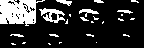
\includegraphics[width=8cm]{imagenes/umbral_binarizada.png}\\
		\caption{Huella facial binarizada}
		\label{fig:thr_binarization}
	\end{figure}

	\item{El truncado necesita como parámetros la imagen y el valor umbral, y formalmente se definiría de la siguiente manera:}
	\[
		thr(I,T) = \begin{cases}
				0, & \text{si $I_{x,y} < T$}\\
				T & \text{si $I_{x,y} \geq T$}
			\end{cases}
	\]
	\begin{figure}[h!]
		\centering
		
\includegraphics[width=8cm]{imagenes/umbral_truncada.png}\\
		\caption{Huella facial truncada}
		\label{fig:thr_truncate}
	\end{figure}

	\item{La reducción a cero necesita como parámetros la imagen y el valor umbral, y formalmente se definiría de la siguiente manera:}
	\[
		thr(I,T) = \begin{cases}
				0, & \text{si $I_{x,y} < T$}\\
				I_{x,y}, & \text{si $I_{x,y} \geq T$}
			\end{cases}
	\]

	\begin{figure}[h!]
		\centering
		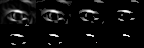
\includegraphics[width=8cm]{imagenes/umbral_tozero.png}\\
		\caption{Huella facial con nivel a 0}
		\label{fig:thr_tozero}
	\end{figure}

\end{itemize}

Para el proyecto se ha acabado empleando la binarización, debido a que:
\begin{itemize}
\item {Las diferencias en los resultados entre un tipo y otro de umbralización eran despreciables.}
\item {Gracias a la binarización se puede comprimir el tamaño de las signatures haciendo la siguiente transformación, donde F es la face signature y R sería el resultado:
\[
 \begin{cases}
	F(x,y)=0 & R(x,y)=0 \\
	F(x,y)=255 & R(x,y)=1
 \end{cases}
\]
Lo cual reduciría el tamaño de la signature a 1/8 de la original\footnote{Esta vendría siendo una aplicación sencilla del algoritmo de Huffman para la compresión de datos.}. }
\end{itemize}


\subsubsection{Suavizado}
El suavizado de una imagen (\textit{smooth} en inglés) consiste en reducir las diferencias entre píxeles colindantes, con lo que el resultado de la operación vendría a ser la imagen desenfocada o ``difuminada''. Existen varios métodos para suavizar una imagen, pero el más común es convolucionar con una gaussiana. Para que esta operación sea lo suficientemente rápida, el kernel de la gaussiana debe de tener valores comunes (3x3, 5x5, 7x7).
Para el suavizado de las huellas faciales se ha empleado el kernel de una gaussiana 3x3 estándar, que es el siguiente:

\[
G(X,Y) = \left(
\begin{array}{lcr}
	\frac{1}{16} & \frac{2}{16} & \frac{1}{16}\\
	\frac{2}{16} & \frac{4}{16} & \frac{2}{16}\\
	\frac{1}{16} & \frac{2}{16} & \frac{1}{16}
\end{array}
\right) = \left(
\begin{array}{lcr}
	\frac{1}{16} & \frac{1}{8} & \frac{1}{16}\\
	\frac{1}{8} & \frac{1}{4} & \frac{1}{8}\\
	\frac{1}{16} & \frac{1}{8} & \frac{1}{16}
\end{array} \right)
\]

Para acelerar el proceso, teniendo en cuenta que la gaussiana es una matriz separable (es el producto de otras dos matrices), se puede convolucionar la imagen con dos kernels diferenciados, uno para la componente vertical y otro para la componente horizontal:
\[
G(X,Y) = \left[
\begin{array}{lcr}
	\frac{1}{16} & \frac{2}{16} & \frac{1}{16}\\
	\frac{2}{16} & \frac{4}{16} & \frac{2}{16}\\
	\frac{1}{16} & \frac{2}{16} & \frac{1}{16}
\end{array}
\right] = \left[
\begin{array}{c}
	\frac{1}{4} \\ \frac{2}{4} \\ \frac{1}{4}
\end{array}
\right]
\left[
\begin{array}{lcr}
	\frac{1}{4} & \frac{2}{4} & \frac{1}{4}
\end{array}
\right]
\]
Que con las extensiones vectoriales de las que disponen hoy día casi todos los procesadores y operaciones de desplazamiento es mucho más rápido de realizar que la convolución por el kernel de 3x3. El resultado de convolucionar una face signature se muestra en la figura \ref{fig:smooth}: a la izquierda de la imagen se puede ver la face signature original, y de izquierda a derecha, se puede observar el suavizado con una gaussiana de 3x3, 5x5 y 7x7, respectivamente.

	\begin{figure}[h!]
		\centering
		
\includegraphics[width=8cm]{imagenes/suavizado.png}\\
		\caption{Suavizado de imagen}
		\label{fig:smooth}
	\end{figure}



\subsection{Comparación entre huellas faciales}

Se han probado diversas medidas de disimilitud entre las huellas faciales extraídas:
\begin{itemize}
	\item{Distancia Euclídea ponderada (distancia euclídea entre huellas faciales ponderada)}
	\item{Distancia And/Or (cociente entre el sumatorio de la and y la or de las huellas faciales)}
	\item{Distancia Xor/Or (cociente entre la or exclusiva y la or lógica de las huellas faciales)}
\end{itemize}
Para facilitar la búsqueda de diferencias, se han probado todas las medidas de similitud umbralizando bajo diferentes valores las imágenes.
Las medidas de disimilitud se detallan a continuación.
\subsubsection{Distancia euclídea ponderada}
La distancia euclídea es una ``clásica'' para la comparación entre dos señales o similares. Aquí se ha ponderado, empleando la siguiente expresión:
\[
D_{euc}(m,n)=\frac{\sum_{i,j=0}^{X,Y}{\sqrt{(m_{i,j}-n_{i,j})^2}}}{XY}
\]
Donde $m$ y $n$ son las imágenes y $X$ e $Y$ son el ancho y el alto de éstas. La ponderación viene dada tras la división entre el tamaño de la imagen (el denominador de la fracción). Aunque en vistas a la eficiencia, si tenemos en cuenta que la elevación al cuadrado y la raíz cuadrada se hacen únicamente para evitar que valores positivos y negativos modifiquen el resultado tenemos la siguiente expresión, que ha sido la empleada:
\[
D_{euc}(m,n)=\frac{\sum_{i,j=0}^{X,Y}{\parallel m_{i,j}-n_{i,j}\parallel}}{XY}
\]
donde $\parallel$ es el valor absoluto de la resta ``píxel a píxel'' entre imágenes. Esta medida tiene las siguientes características:
\begin{itemize}
	\item{$D_{euc}\in\mathbb{R}_{0,255}$ (el valor de $D_{euc}$ es un natural en el intervalo $\left[0,255\right]$)} 
	\item{Es conmutativa por definición ($D_{euc}(i,j)=D_{euc}(j,i)$)}
	\item{Es una medida de disimilitud, es decir, que $D_{euc}(i,j) > D_{euc} (i,k)$ significaría que $i$ es más similar a $k$ que $j$}
	\item{Esta ha sido la medida escogida para filtrados superpuestos, con un umbral de 16. Ha demostrado un comportamiento razonable con respecto al resto de alternativas.}
\end{itemize}

A continuación tenemos un ejemplo de cómo calcularla. Si disponemos de las siguientes matrices simulando imágenes de 1 byte per píxel:
\[ M=\left( \begin{array}{lcr}
	255 & 127 & 255 \\
	0 & 0 & 255 \\
	255 & 0 & 0 
\end{array} \right), N=\left( \begin{array}{lcr}
	255 & 255 & 0 \\
	0 & 255 & 255 \\
	255 & 0 & 127 
\end{array} \right) 
\]
Entonces tendríamos que 
\[D_{euc}(M,N) = \frac
	{\sum_{i,j=0}^{3,3}\left( 
		\begin{array}{lcr}
			0 & 128 & 255\\ 0 & 255 & 0 \\ 0 & 0 & 127 
		\end{array} 
	\right)}
	{9} = 85
\]
La distancia euclídea como tal entre una imagen y otra es 85. Podríamos pasarla a un intervalo $p \in \mathbb{R}_{0..1}$ mediante una interpolación sencilla:
\[
	p = \frac{D_{euc}}{255}
\]
y en este caso la distancia entre matrices sería $D_{euc}=\frac{85}{255}\approx0,333$, lo cual nos indicaría que la disimilitud entre ambas imágenes es aproximadamente del 33,3\%. Por otro lado, trabajar con números naturales por norma general suele ser menos costoso para la CPU, así que se ha trasladado el resultado de $\mathbb{R}_{0,255}$ a $\mathbb{N}_{0,255}$.

\subsubsection{Distancia And/Or}
La distancia And/Or se ha calculado de la siguiente manera:
\[
D_{and}(m,n)=\frac{ \sum_{x,y=0}^{X,Y}(m_{x,y} \wedge n_{x,y}) }{ \sum_{x,y=0}^{X,Y}(m_{x,y} \vee n_{x,y}) }
\]
El operador $\wedge$ representa la and (y lógica) bit a bit entre píxel y píxel de la imagen, y el operador $\vee$ la or (o lógica) entre píxeles. 
\begin{itemize}
	\item{$D_{and}\in\mathbb{R}_{\left[0,1\right]}$ (el valor de $D_{and}$ es un real en el intervalo $\left[0,1\right]$)} 
	\item{Es conmutativa por definición ($D_{and}(i,j)=D_{and}(j,i)$)}
	\item{Es una medida de similitud, es decir, que $D_{and}(i,j) > D_{and} (i,k)$ significaría que $i$ es más similar a $j$ que $k$}
	\item{Esta medida ha demostrado un comportamiento inesperadamente inválido\footnote{Se cree que debe de ser por un conjunto de outliers en las comparaciones intergrupo, no en vano son un orden de magnitud superior a las comparaciones intragrupo.}}
\end{itemize}

Por ejemplo, si disponemos de las matrices del caso anterior:
\[ M=\left( \begin{array}{lcr}
	255 & 127 & 255 \\
	0 & 0 & 255 \\
	255 & 0 & 0 
\end{array} \right), N=\left( \begin{array}{lcr}
	255 & 255 & 0 \\
	0 & 255 & 255 \\
	255 & 0 & 127 
\end{array} \right) 
\]

Para calcular la $D_{and}(M.N)$ necesitaríamos calcular inicialmente $M \wedge N$ y $M \vee N$
\[ (M \wedge N)=\left( \begin{array}{lcr}
	255 & 127 & 0 \\
	0 & 0 & 255 \\
	255 & 0 & 0 
\end{array} \right), (M \vee N)=\left( \begin{array}{lcr}
	255 & 255 & 255 \\
	0 & 255 & 255 \\
	255 & 0 & 127 
\end{array} \right) 
\]

El cálculo de la distancia se haría a partir de ambos sumatorios:
\[D_{and}(M,N) = \frac 
	{\sum_{i,j=0}^{3,3} M \wedge N} 
	{\sum_{i,j=0}^{3,3} M \vee N} = \frac {892}{1657} = 0,538322269 
\]
Si hacemos la aproximación $ 0,538322269 \approx 0,54 $ tenemos que ambas matrices tienen un índice de similitud del 54\%.

\subsubsection{Distancia Xor/Or}
La distancia Xor/Or se ha calculado de la siguiente manera:
\[
D_{xor}(m,n)=\frac{ \sum_{x,y=0}^{X,Y}(m_{x,y} \oplus n_{x,y}) }{ \sum_{x,y=0}^{X,Y}(m_{x,y} \vee n_{x,y}) }
\]
En este caso el operador $\oplus$ representa la or exclusiva (XOR) entre píxel y píxel de la imagen, y el operador $\vee$, de igual manera que antes, la OR entre ambos.
\begin{itemize}
	\item{$D_{xor}\in\mathbb{R}_{\left[0,1\right]}$ (el valor de $D_{xor}$ es un real en el intervalo $\left[0,1\right]$)} 
	\item{Es conmutativa por definición ($D_{xor}(i,j)=D_{xor}(j,i)$)}
	\item{Es una medida de disimilitud, es decir, que $D_{xor}(i,j) > D_{xor} (i,k)$ significaría que $i$ es más similar a $k$ que $j$}
	\item{Esta distancia no se ha escogido porque aún a pesar de dar buenos resultados (de hecho tenía una variabilidad inferior a la euclídea) seguía estando por debajo de la distancia euclídea en el caso de que los filtrados fuesen superpuestos. Para filtrados concatenados, su calidad es superior a la de la distancia euclídea}

\end{itemize}
Por ejemplo, para calcular la distancia XOR/OR $D_{xor}$ de las matrices (representando imágenes) del caso anterior:
\[ M=\left( \begin{array}{lcr}
	255 & 127 & 255 \\
	0 & 0 & 255 \\
	255 & 0 & 0 
\end{array} \right), N=\left( \begin{array}{lcr}
	255 & 255 & 0 \\
	0 & 255 & 255 \\
	255 & 0 & 127 
\end{array} \right) 
\]

Para calcular la $D_{xor}(M.N)$ utilizaremos $M \oplus N$ y $M \vee N$ (que será la misma que en $D_{and}$)
\[ (M \oplus N)=\left( \begin{array}{lcr}
	0 & 128 & 255 \\
	0 & 255 & 0 \\
	0 & 0 & 127 
\end{array} \right), (M \vee N)=\left( \begin{array}{lcr}
	255 & 255 & 255 \\
	0 & 255 & 255 \\
	255 & 0 & 127 
\end{array} \right) 
\]

El cálculo de la distancia se haría a partir de ambos sumatorios:
\[D_{xor}(M,N) = \frac 
	{\sum_{i,j=0}^{3,3} M \oplus N} 
	{\sum_{i,j=0}^{3,3} M \vee N} = \frac {765}{1657} = 0,461677731
\]
Si hacemos la aproximación $ 0,461677731 \approx 0,46 $ tenemos que ambas matrices tienen un índice de disimilitud del 46\%.


\subsection{Identificación}
Como se ha comentado previamente, se ha decidido emplear la distancia Euclídea sobre filtrados superpuestos y con un umbral de 16. Para el proceso de identificación no se ha implementado ningún tipo de indexado ni similares (full scan), así que los tiempos de búsqueda de individuos degenerarían linealmente ( $O(n)$ ) según el número de individuos dados de alta se incrementase.

\chapter{Resultados obtenidos}

\section{Consideraciones previas}

\subsection{Juegos de pruebas}
Para realizar las pruebas de reconocimiento facial se han empleado las imágenes que la universidad tecnológica de California alberga en 
\begin{verbatim}
http://www.vision.caltech.edu/Image_Datasets/faces/faces.tar 
\end{verbatim}
Es un fichero tar que cuenta con 451 imágenes frontales de aproximadamente 27 individuos (32 si contamos varios dibujos e individuos sin suficientes fotografías como para poder comprobar problemas intragrupo). Se ha decidido emplear este conjunto de imágenes por los siguientes motivos:
\begin{itemize}
	\item{Número suficiente de imágenes y de individuos como para poder considerar los resultados aceptables mediante estadística.}
	\item{Condiciones variables de luminosidad y de enfoque. Tenemos la posibilidad de comprobar la robustez del reconocimiento facial en condiciones variadas.}
	\item{Fondos de la fotografía variados. Gracias a esta característica podemos comprobar con facilidad la tasa de falsos positivos en la detección facial.}
	\item{Buena resolución de las imágenes capturadas: cada fotografía es un JPG de 896x592 píxeles, que es una mayor resolución incluso que la que obtenemos con la cámara empleada (640x480), así que el tiempo de procesado es comparable al de la imagen capturada.\footnote{El tiempo de captura de imagen vía cámara no es despreciable y añade un overheading al respecto.} }
\end{itemize}

Sobre este subconjunto de imágenes se tomarán las estadísticas de calidad de funcionamiento (Tasa de falsos rechazos/Tasa de falsos aciertos) y rendimiento (Tiempo de ejecución).

\subsection{Conceptos estadísticos empleados}
Para el análisis estadístico realizado se han empleado los conceptos definidos a continuación:
\begin{itemize}
	\item{La \textbf{tasa de falsa aceptación (TFA)}\footnote{En inglés conocida como \textbf{False acceptation rate (FAR)}.} se define como el porcentaje de muestras en las que se ha extraído un falso positivo o una falsa identificación. La TFA mide la robustez del sistema.}
	\item{La \textbf{tasa de falso rechazo (TFR)}\footnote{En inglés conocida como \textbf{False rejection rate (FRR)}.} se define como el porcentaje de muestras en las que debiendo dar un resultado positivo, se devuelve un resultado negativo. La TFR mide la "comodidad de uso" del sistema en el sentido de que por parte del usuario no sea necesaria mayor interacción de la requerida. }
\end {itemize}

En este proyecto la TFA se calcularía a partir del número de individuos reconocidos como otro cualquiera mientras que la TFR se calcula a partir de las muestras que no reconocen al individuo aún estando situado frente a la cámara.

Cuando ambos porcentajes dependen de una variable (supongamos un umbral cualquiera como pueda ser grado de igualdad, tamaño de muestra, etc.) se representan en gráficas TFA/TFR. El punto óptimo de trabajo es aquel en el que se minimiza la TFA mientras la TFR se mantiene en valores aceptables que coincide con el punto donde ambas curvas se cruzan, pero sacrificando uno de los dos aspectos se puede adaptar el sistema a otros entornos.

\newpage

\section{Estadísticas}

Las estadísticas a tomar son las siguientes:

\subsection{Estadísticas en localización facial}
El algoritmo empleado es eficiente y eficaz. Hubo 5 falsos negativos sobre 451 imágenes. Sobre las 446 restantes, se hallaron 69 falsos positivos. 

\newpage

\section{Eficiencia en máquina}
\subsection{Tiempos de ejecución}
%stats_carga_imagen.tex
\begin{figure}[h!]
        \centering
        % GNUPLOT: LaTeX picture
\setlength{\unitlength}{0.240900pt}
\ifx\plotpoint\undefined\newsavebox{\plotpoint}\fi
\sbox{\plotpoint}{\rule[-0.200pt]{0.400pt}{0.400pt}}%
\begin{picture}(1500,900)(0,0)
\sbox{\plotpoint}{\rule[-0.200pt]{0.400pt}{0.400pt}}%
\put(231.0,131.0){\rule[-0.200pt]{4.818pt}{0.400pt}}
\put(211,131){\makebox(0,0)[r]{ 0}}
\put(1430.0,131.0){\rule[-0.200pt]{4.818pt}{0.400pt}}
\put(231.0,203.0){\rule[-0.200pt]{4.818pt}{0.400pt}}
\put(211,203){\makebox(0,0)[r]{ 0.01}}
\put(1430.0,203.0){\rule[-0.200pt]{4.818pt}{0.400pt}}
\put(231.0,275.0){\rule[-0.200pt]{4.818pt}{0.400pt}}
\put(211,275){\makebox(0,0)[r]{ 0.02}}
\put(1430.0,275.0){\rule[-0.200pt]{4.818pt}{0.400pt}}
\put(231.0,346.0){\rule[-0.200pt]{4.818pt}{0.400pt}}
\put(211,346){\makebox(0,0)[r]{ 0.03}}
\put(1430.0,346.0){\rule[-0.200pt]{4.818pt}{0.400pt}}
\put(231.0,418.0){\rule[-0.200pt]{4.818pt}{0.400pt}}
\put(211,418){\makebox(0,0)[r]{ 0.04}}
\put(1430.0,418.0){\rule[-0.200pt]{4.818pt}{0.400pt}}
\put(231.0,490.0){\rule[-0.200pt]{4.818pt}{0.400pt}}
\put(211,490){\makebox(0,0)[r]{ 0.05}}
\put(1430.0,490.0){\rule[-0.200pt]{4.818pt}{0.400pt}}
\put(231.0,562.0){\rule[-0.200pt]{4.818pt}{0.400pt}}
\put(211,562){\makebox(0,0)[r]{ 0.06}}
\put(1430.0,562.0){\rule[-0.200pt]{4.818pt}{0.400pt}}
\put(231.0,633.0){\rule[-0.200pt]{4.818pt}{0.400pt}}
\put(211,633){\makebox(0,0)[r]{ 0.07}}
\put(1430.0,633.0){\rule[-0.200pt]{4.818pt}{0.400pt}}
\put(231.0,705.0){\rule[-0.200pt]{4.818pt}{0.400pt}}
\put(211,705){\makebox(0,0)[r]{ 0.08}}
\put(1430.0,705.0){\rule[-0.200pt]{4.818pt}{0.400pt}}
\put(231.0,777.0){\rule[-0.200pt]{4.818pt}{0.400pt}}
\put(211,777){\makebox(0,0)[r]{ 0.09}}
\put(1430.0,777.0){\rule[-0.200pt]{4.818pt}{0.400pt}}
\put(231.0,131.0){\rule[-0.200pt]{0.400pt}{4.818pt}}
\put(231,90){\makebox(0,0){ 0}}
\put(231.0,757.0){\rule[-0.200pt]{0.400pt}{4.818pt}}
\put(475.0,131.0){\rule[-0.200pt]{0.400pt}{4.818pt}}
\put(475,90){\makebox(0,0){ 500}}
\put(475.0,757.0){\rule[-0.200pt]{0.400pt}{4.818pt}}
\put(719.0,131.0){\rule[-0.200pt]{0.400pt}{4.818pt}}
\put(719,90){\makebox(0,0){ 1000}}
\put(719.0,757.0){\rule[-0.200pt]{0.400pt}{4.818pt}}
\put(962.0,131.0){\rule[-0.200pt]{0.400pt}{4.818pt}}
\put(962,90){\makebox(0,0){ 1500}}
\put(962.0,757.0){\rule[-0.200pt]{0.400pt}{4.818pt}}
\put(1206.0,131.0){\rule[-0.200pt]{0.400pt}{4.818pt}}
\put(1206,90){\makebox(0,0){ 2000}}
\put(1206.0,757.0){\rule[-0.200pt]{0.400pt}{4.818pt}}
\put(1450.0,131.0){\rule[-0.200pt]{0.400pt}{4.818pt}}
\put(1450,90){\makebox(0,0){ 2500}}
\put(1450.0,757.0){\rule[-0.200pt]{0.400pt}{4.818pt}}
\put(231.0,131.0){\rule[-0.200pt]{0.400pt}{155.621pt}}
\put(231.0,131.0){\rule[-0.200pt]{293.657pt}{0.400pt}}
\put(1450.0,131.0){\rule[-0.200pt]{0.400pt}{155.621pt}}
\put(231.0,777.0){\rule[-0.200pt]{293.657pt}{0.400pt}}
\put(70,454){\makebox(0,0){Segundos}}
\put(840,29){\makebox(0,0){Muestras}}
\put(840,839){\makebox(0,0){Carga de imagen}}
\put(1290,737){\makebox(0,0)[r]{Tcarga}}
\put(231,259){\makebox(0,0){$+$}}
\put(231,256){\makebox(0,0){$+$}}
\put(232,255){\makebox(0,0){$+$}}
\put(232,257){\makebox(0,0){$+$}}
\put(233,264){\makebox(0,0){$+$}}
\put(233,257){\makebox(0,0){$+$}}
\put(234,261){\makebox(0,0){$+$}}
\put(234,247){\makebox(0,0){$+$}}
\put(235,247){\makebox(0,0){$+$}}
\put(235,260){\makebox(0,0){$+$}}
\put(236,247){\makebox(0,0){$+$}}
\put(236,252){\makebox(0,0){$+$}}
\put(237,251){\makebox(0,0){$+$}}
\put(237,255){\makebox(0,0){$+$}}
\put(238,261){\makebox(0,0){$+$}}
\put(238,253){\makebox(0,0){$+$}}
\put(239,247){\makebox(0,0){$+$}}
\put(239,245){\makebox(0,0){$+$}}
\put(240,257){\makebox(0,0){$+$}}
\put(240,252){\makebox(0,0){$+$}}
\put(241,274){\makebox(0,0){$+$}}
\put(241,258){\makebox(0,0){$+$}}
\put(242,261){\makebox(0,0){$+$}}
\put(242,275){\makebox(0,0){$+$}}
\put(243,274){\makebox(0,0){$+$}}
\put(243,264){\makebox(0,0){$+$}}
\put(244,268){\makebox(0,0){$+$}}
\put(244,259){\makebox(0,0){$+$}}
\put(245,265){\makebox(0,0){$+$}}
\put(245,271){\makebox(0,0){$+$}}
\put(246,245){\makebox(0,0){$+$}}
\put(246,263){\makebox(0,0){$+$}}
\put(247,267){\makebox(0,0){$+$}}
\put(247,261){\makebox(0,0){$+$}}
\put(248,402){\makebox(0,0){$+$}}
\put(248,274){\makebox(0,0){$+$}}
\put(249,271){\makebox(0,0){$+$}}
\put(249,254){\makebox(0,0){$+$}}
\put(250,259){\makebox(0,0){$+$}}
\put(250,275){\makebox(0,0){$+$}}
\put(251,261){\makebox(0,0){$+$}}
\put(251,264){\makebox(0,0){$+$}}
\put(251,254){\makebox(0,0){$+$}}
\put(252,262){\makebox(0,0){$+$}}
\put(252,258){\makebox(0,0){$+$}}
\put(253,257){\makebox(0,0){$+$}}
\put(253,270){\makebox(0,0){$+$}}
\put(254,271){\makebox(0,0){$+$}}
\put(254,262){\makebox(0,0){$+$}}
\put(255,254){\makebox(0,0){$+$}}
\put(255,254){\makebox(0,0){$+$}}
\put(256,252){\makebox(0,0){$+$}}
\put(256,255){\makebox(0,0){$+$}}
\put(257,257){\makebox(0,0){$+$}}
\put(257,255){\makebox(0,0){$+$}}
\put(258,258){\makebox(0,0){$+$}}
\put(258,263){\makebox(0,0){$+$}}
\put(259,248){\makebox(0,0){$+$}}
\put(259,250){\makebox(0,0){$+$}}
\put(260,254){\makebox(0,0){$+$}}
\put(260,258){\makebox(0,0){$+$}}
\put(261,262){\makebox(0,0){$+$}}
\put(261,258){\makebox(0,0){$+$}}
\put(262,252){\makebox(0,0){$+$}}
\put(262,248){\makebox(0,0){$+$}}
\put(263,260){\makebox(0,0){$+$}}
\put(263,245){\makebox(0,0){$+$}}
\put(264,257){\makebox(0,0){$+$}}
\put(264,254){\makebox(0,0){$+$}}
\put(265,253){\makebox(0,0){$+$}}
\put(265,135){\makebox(0,0){$+$}}
\put(266,258){\makebox(0,0){$+$}}
\put(266,261){\makebox(0,0){$+$}}
\put(267,259){\makebox(0,0){$+$}}
\put(267,266){\makebox(0,0){$+$}}
\put(268,252){\makebox(0,0){$+$}}
\put(268,259){\makebox(0,0){$+$}}
\put(269,256){\makebox(0,0){$+$}}
\put(269,259){\makebox(0,0){$+$}}
\put(270,269){\makebox(0,0){$+$}}
\put(270,258){\makebox(0,0){$+$}}
\put(270,253){\makebox(0,0){$+$}}
\put(271,251){\makebox(0,0){$+$}}
\put(271,259){\makebox(0,0){$+$}}
\put(272,259){\makebox(0,0){$+$}}
\put(272,254){\makebox(0,0){$+$}}
\put(273,259){\makebox(0,0){$+$}}
\put(273,256){\makebox(0,0){$+$}}
\put(274,261){\makebox(0,0){$+$}}
\put(274,257){\makebox(0,0){$+$}}
\put(275,249){\makebox(0,0){$+$}}
\put(275,241){\makebox(0,0){$+$}}
\put(276,252){\makebox(0,0){$+$}}
\put(276,254){\makebox(0,0){$+$}}
\put(277,257){\makebox(0,0){$+$}}
\put(277,256){\makebox(0,0){$+$}}
\put(278,254){\makebox(0,0){$+$}}
\put(278,261){\makebox(0,0){$+$}}
\put(279,260){\makebox(0,0){$+$}}
\put(279,260){\makebox(0,0){$+$}}
\put(280,258){\makebox(0,0){$+$}}
\put(280,256){\makebox(0,0){$+$}}
\put(281,265){\makebox(0,0){$+$}}
\put(281,264){\makebox(0,0){$+$}}
\put(282,254){\makebox(0,0){$+$}}
\put(282,254){\makebox(0,0){$+$}}
\put(283,256){\makebox(0,0){$+$}}
\put(283,252){\makebox(0,0){$+$}}
\put(284,259){\makebox(0,0){$+$}}
\put(284,263){\makebox(0,0){$+$}}
\put(285,259){\makebox(0,0){$+$}}
\put(285,254){\makebox(0,0){$+$}}
\put(286,264){\makebox(0,0){$+$}}
\put(286,250){\makebox(0,0){$+$}}
\put(287,251){\makebox(0,0){$+$}}
\put(287,248){\makebox(0,0){$+$}}
\put(288,258){\makebox(0,0){$+$}}
\put(288,254){\makebox(0,0){$+$}}
\put(289,260){\makebox(0,0){$+$}}
\put(289,250){\makebox(0,0){$+$}}
\put(290,263){\makebox(0,0){$+$}}
\put(290,254){\makebox(0,0){$+$}}
\put(290,258){\makebox(0,0){$+$}}
\put(291,254){\makebox(0,0){$+$}}
\put(291,261){\makebox(0,0){$+$}}
\put(292,257){\makebox(0,0){$+$}}
\put(292,260){\makebox(0,0){$+$}}
\put(293,253){\makebox(0,0){$+$}}
\put(293,254){\makebox(0,0){$+$}}
\put(294,252){\makebox(0,0){$+$}}
\put(294,262){\makebox(0,0){$+$}}
\put(295,254){\makebox(0,0){$+$}}
\put(295,268){\makebox(0,0){$+$}}
\put(296,258){\makebox(0,0){$+$}}
\put(296,260){\makebox(0,0){$+$}}
\put(297,257){\makebox(0,0){$+$}}
\put(297,258){\makebox(0,0){$+$}}
\put(298,267){\makebox(0,0){$+$}}
\put(298,265){\makebox(0,0){$+$}}
\put(299,256){\makebox(0,0){$+$}}
\put(299,254){\makebox(0,0){$+$}}
\put(300,264){\makebox(0,0){$+$}}
\put(300,241){\makebox(0,0){$+$}}
\put(301,248){\makebox(0,0){$+$}}
\put(301,260){\makebox(0,0){$+$}}
\put(302,253){\makebox(0,0){$+$}}
\put(302,250){\makebox(0,0){$+$}}
\put(303,262){\makebox(0,0){$+$}}
\put(303,257){\makebox(0,0){$+$}}
\put(304,261){\makebox(0,0){$+$}}
\put(304,257){\makebox(0,0){$+$}}
\put(305,260){\makebox(0,0){$+$}}
\put(305,253){\makebox(0,0){$+$}}
\put(306,259){\makebox(0,0){$+$}}
\put(306,258){\makebox(0,0){$+$}}
\put(307,261){\makebox(0,0){$+$}}
\put(307,255){\makebox(0,0){$+$}}
\put(308,262){\makebox(0,0){$+$}}
\put(308,258){\makebox(0,0){$+$}}
\put(309,262){\makebox(0,0){$+$}}
\put(309,259){\makebox(0,0){$+$}}
\put(310,265){\makebox(0,0){$+$}}
\put(310,256){\makebox(0,0){$+$}}
\put(310,261){\makebox(0,0){$+$}}
\put(311,261){\makebox(0,0){$+$}}
\put(311,265){\makebox(0,0){$+$}}
\put(312,249){\makebox(0,0){$+$}}
\put(312,253){\makebox(0,0){$+$}}
\put(313,250){\makebox(0,0){$+$}}
\put(313,240){\makebox(0,0){$+$}}
\put(314,255){\makebox(0,0){$+$}}
\put(314,245){\makebox(0,0){$+$}}
\put(315,252){\makebox(0,0){$+$}}
\put(315,254){\makebox(0,0){$+$}}
\put(316,257){\makebox(0,0){$+$}}
\put(316,255){\makebox(0,0){$+$}}
\put(317,251){\makebox(0,0){$+$}}
\put(317,252){\makebox(0,0){$+$}}
\put(318,254){\makebox(0,0){$+$}}
\put(318,264){\makebox(0,0){$+$}}
\put(319,258){\makebox(0,0){$+$}}
\put(319,251){\makebox(0,0){$+$}}
\put(320,255){\makebox(0,0){$+$}}
\put(320,258){\makebox(0,0){$+$}}
\put(321,265){\makebox(0,0){$+$}}
\put(321,256){\makebox(0,0){$+$}}
\put(322,262){\makebox(0,0){$+$}}
\put(322,257){\makebox(0,0){$+$}}
\put(323,263){\makebox(0,0){$+$}}
\put(323,272){\makebox(0,0){$+$}}
\put(324,262){\makebox(0,0){$+$}}
\put(324,268){\makebox(0,0){$+$}}
\put(325,264){\makebox(0,0){$+$}}
\put(325,248){\makebox(0,0){$+$}}
\put(326,260){\makebox(0,0){$+$}}
\put(326,260){\makebox(0,0){$+$}}
\put(327,371){\makebox(0,0){$+$}}
\put(327,357){\makebox(0,0){$+$}}
\put(328,303){\makebox(0,0){$+$}}
\put(328,457){\makebox(0,0){$+$}}
\put(329,297){\makebox(0,0){$+$}}
\put(329,339){\makebox(0,0){$+$}}
\put(329,307){\makebox(0,0){$+$}}
\put(330,397){\makebox(0,0){$+$}}
\put(330,368){\makebox(0,0){$+$}}
\put(331,275){\makebox(0,0){$+$}}
\put(331,292){\makebox(0,0){$+$}}
\put(332,305){\makebox(0,0){$+$}}
\put(332,269){\makebox(0,0){$+$}}
\put(333,331){\makebox(0,0){$+$}}
\put(333,266){\makebox(0,0){$+$}}
\put(334,269){\makebox(0,0){$+$}}
\put(334,265){\makebox(0,0){$+$}}
\put(335,338){\makebox(0,0){$+$}}
\put(335,269){\makebox(0,0){$+$}}
\put(336,314){\makebox(0,0){$+$}}
\put(336,264){\makebox(0,0){$+$}}
\put(337,320){\makebox(0,0){$+$}}
\put(337,265){\makebox(0,0){$+$}}
\put(338,260){\makebox(0,0){$+$}}
\put(338,399){\makebox(0,0){$+$}}
\put(339,431){\makebox(0,0){$+$}}
\put(339,267){\makebox(0,0){$+$}}
\put(340,432){\makebox(0,0){$+$}}
\put(340,352){\makebox(0,0){$+$}}
\put(341,323){\makebox(0,0){$+$}}
\put(341,342){\makebox(0,0){$+$}}
\put(342,348){\makebox(0,0){$+$}}
\put(342,408){\makebox(0,0){$+$}}
\put(343,380){\makebox(0,0){$+$}}
\put(343,276){\makebox(0,0){$+$}}
\put(344,291){\makebox(0,0){$+$}}
\put(344,271){\makebox(0,0){$+$}}
\put(345,282){\makebox(0,0){$+$}}
\put(345,276){\makebox(0,0){$+$}}
\put(346,299){\makebox(0,0){$+$}}
\put(346,265){\makebox(0,0){$+$}}
\put(347,244){\makebox(0,0){$+$}}
\put(347,265){\makebox(0,0){$+$}}
\put(348,286){\makebox(0,0){$+$}}
\put(348,270){\makebox(0,0){$+$}}
\put(349,258){\makebox(0,0){$+$}}
\put(349,268){\makebox(0,0){$+$}}
\put(349,263){\makebox(0,0){$+$}}
\put(350,325){\makebox(0,0){$+$}}
\put(350,297){\makebox(0,0){$+$}}
\put(351,265){\makebox(0,0){$+$}}
\put(351,382){\makebox(0,0){$+$}}
\put(352,282){\makebox(0,0){$+$}}
\put(352,313){\makebox(0,0){$+$}}
\put(353,320){\makebox(0,0){$+$}}
\put(353,267){\makebox(0,0){$+$}}
\put(354,361){\makebox(0,0){$+$}}
\put(354,269){\makebox(0,0){$+$}}
\put(355,334){\makebox(0,0){$+$}}
\put(355,322){\makebox(0,0){$+$}}
\put(356,342){\makebox(0,0){$+$}}
\put(356,319){\makebox(0,0){$+$}}
\put(357,272){\makebox(0,0){$+$}}
\put(357,265){\makebox(0,0){$+$}}
\put(358,264){\makebox(0,0){$+$}}
\put(358,294){\makebox(0,0){$+$}}
\put(359,323){\makebox(0,0){$+$}}
\put(359,332){\makebox(0,0){$+$}}
\put(360,275){\makebox(0,0){$+$}}
\put(360,255){\makebox(0,0){$+$}}
\put(361,275){\makebox(0,0){$+$}}
\put(361,269){\makebox(0,0){$+$}}
\put(362,267){\makebox(0,0){$+$}}
\put(362,330){\makebox(0,0){$+$}}
\put(363,265){\makebox(0,0){$+$}}
\put(363,263){\makebox(0,0){$+$}}
\put(364,268){\makebox(0,0){$+$}}
\put(364,265){\makebox(0,0){$+$}}
\put(365,264){\makebox(0,0){$+$}}
\put(365,265){\makebox(0,0){$+$}}
\put(366,337){\makebox(0,0){$+$}}
\put(366,310){\makebox(0,0){$+$}}
\put(367,324){\makebox(0,0){$+$}}
\put(367,317){\makebox(0,0){$+$}}
\put(368,269){\makebox(0,0){$+$}}
\put(368,311){\makebox(0,0){$+$}}
\put(369,340){\makebox(0,0){$+$}}
\put(369,272){\makebox(0,0){$+$}}
\put(369,384){\makebox(0,0){$+$}}
\put(370,257){\makebox(0,0){$+$}}
\put(370,259){\makebox(0,0){$+$}}
\put(371,328){\makebox(0,0){$+$}}
\put(371,271){\makebox(0,0){$+$}}
\put(372,264){\makebox(0,0){$+$}}
\put(372,289){\makebox(0,0){$+$}}
\put(373,252){\makebox(0,0){$+$}}
\put(373,259){\makebox(0,0){$+$}}
\put(374,259){\makebox(0,0){$+$}}
\put(374,269){\makebox(0,0){$+$}}
\put(375,340){\makebox(0,0){$+$}}
\put(375,270){\makebox(0,0){$+$}}
\put(376,277){\makebox(0,0){$+$}}
\put(376,369){\makebox(0,0){$+$}}
\put(377,344){\makebox(0,0){$+$}}
\put(377,263){\makebox(0,0){$+$}}
\put(378,256){\makebox(0,0){$+$}}
\put(378,285){\makebox(0,0){$+$}}
\put(379,323){\makebox(0,0){$+$}}
\put(379,340){\makebox(0,0){$+$}}
\put(380,324){\makebox(0,0){$+$}}
\put(380,262){\makebox(0,0){$+$}}
\put(381,271){\makebox(0,0){$+$}}
\put(381,320){\makebox(0,0){$+$}}
\put(382,310){\makebox(0,0){$+$}}
\put(382,270){\makebox(0,0){$+$}}
\put(383,264){\makebox(0,0){$+$}}
\put(383,327){\makebox(0,0){$+$}}
\put(384,277){\makebox(0,0){$+$}}
\put(384,327){\makebox(0,0){$+$}}
\put(385,263){\makebox(0,0){$+$}}
\put(385,254){\makebox(0,0){$+$}}
\put(386,258){\makebox(0,0){$+$}}
\put(386,274){\makebox(0,0){$+$}}
\put(387,293){\makebox(0,0){$+$}}
\put(387,283){\makebox(0,0){$+$}}
\put(388,264){\makebox(0,0){$+$}}
\put(388,274){\makebox(0,0){$+$}}
\put(388,271){\makebox(0,0){$+$}}
\put(389,264){\makebox(0,0){$+$}}
\put(389,303){\makebox(0,0){$+$}}
\put(390,286){\makebox(0,0){$+$}}
\put(390,324){\makebox(0,0){$+$}}
\put(391,314){\makebox(0,0){$+$}}
\put(391,469){\makebox(0,0){$+$}}
\put(392,270){\makebox(0,0){$+$}}
\put(392,296){\makebox(0,0){$+$}}
\put(393,321){\makebox(0,0){$+$}}
\put(393,345){\makebox(0,0){$+$}}
\put(394,273){\makebox(0,0){$+$}}
\put(394,320){\makebox(0,0){$+$}}
\put(395,263){\makebox(0,0){$+$}}
\put(395,280){\makebox(0,0){$+$}}
\put(396,319){\makebox(0,0){$+$}}
\put(396,266){\makebox(0,0){$+$}}
\put(397,289){\makebox(0,0){$+$}}
\put(397,262){\makebox(0,0){$+$}}
\put(398,328){\makebox(0,0){$+$}}
\put(398,293){\makebox(0,0){$+$}}
\put(399,327){\makebox(0,0){$+$}}
\put(399,268){\makebox(0,0){$+$}}
\put(400,375){\makebox(0,0){$+$}}
\put(400,339){\makebox(0,0){$+$}}
\put(401,280){\makebox(0,0){$+$}}
\put(401,266){\makebox(0,0){$+$}}
\put(402,364){\makebox(0,0){$+$}}
\put(402,300){\makebox(0,0){$+$}}
\put(403,266){\makebox(0,0){$+$}}
\put(403,339){\makebox(0,0){$+$}}
\put(404,264){\makebox(0,0){$+$}}
\put(404,272){\makebox(0,0){$+$}}
\put(405,268){\makebox(0,0){$+$}}
\put(405,389){\makebox(0,0){$+$}}
\put(406,261){\makebox(0,0){$+$}}
\put(406,262){\makebox(0,0){$+$}}
\put(407,265){\makebox(0,0){$+$}}
\put(407,265){\makebox(0,0){$+$}}
\put(408,258){\makebox(0,0){$+$}}
\put(408,257){\makebox(0,0){$+$}}
\put(408,258){\makebox(0,0){$+$}}
\put(409,278){\makebox(0,0){$+$}}
\put(409,325){\makebox(0,0){$+$}}
\put(410,286){\makebox(0,0){$+$}}
\put(410,322){\makebox(0,0){$+$}}
\put(411,263){\makebox(0,0){$+$}}
\put(411,291){\makebox(0,0){$+$}}
\put(412,264){\makebox(0,0){$+$}}
\put(412,315){\makebox(0,0){$+$}}
\put(413,267){\makebox(0,0){$+$}}
\put(413,273){\makebox(0,0){$+$}}
\put(414,274){\makebox(0,0){$+$}}
\put(414,285){\makebox(0,0){$+$}}
\put(415,290){\makebox(0,0){$+$}}
\put(415,275){\makebox(0,0){$+$}}
\put(416,260){\makebox(0,0){$+$}}
\put(416,331){\makebox(0,0){$+$}}
\put(417,262){\makebox(0,0){$+$}}
\put(417,292){\makebox(0,0){$+$}}
\put(418,262){\makebox(0,0){$+$}}
\put(418,257){\makebox(0,0){$+$}}
\put(419,264){\makebox(0,0){$+$}}
\put(419,342){\makebox(0,0){$+$}}
\put(420,264){\makebox(0,0){$+$}}
\put(420,338){\makebox(0,0){$+$}}
\put(421,338){\makebox(0,0){$+$}}
\put(421,285){\makebox(0,0){$+$}}
\put(422,268){\makebox(0,0){$+$}}
\put(422,277){\makebox(0,0){$+$}}
\put(423,294){\makebox(0,0){$+$}}
\put(423,285){\makebox(0,0){$+$}}
\put(424,297){\makebox(0,0){$+$}}
\put(424,256){\makebox(0,0){$+$}}
\put(425,263){\makebox(0,0){$+$}}
\put(425,287){\makebox(0,0){$+$}}
\put(426,344){\makebox(0,0){$+$}}
\put(426,306){\makebox(0,0){$+$}}
\put(427,268){\makebox(0,0){$+$}}
\put(427,267){\makebox(0,0){$+$}}
\put(428,265){\makebox(0,0){$+$}}
\put(428,269){\makebox(0,0){$+$}}
\put(428,269){\makebox(0,0){$+$}}
\put(429,266){\makebox(0,0){$+$}}
\put(429,267){\makebox(0,0){$+$}}
\put(430,282){\makebox(0,0){$+$}}
\put(430,287){\makebox(0,0){$+$}}
\put(431,328){\makebox(0,0){$+$}}
\put(431,318){\makebox(0,0){$+$}}
\put(432,262){\makebox(0,0){$+$}}
\put(432,327){\makebox(0,0){$+$}}
\put(433,264){\makebox(0,0){$+$}}
\put(433,297){\makebox(0,0){$+$}}
\put(434,307){\makebox(0,0){$+$}}
\put(434,280){\makebox(0,0){$+$}}
\put(435,254){\makebox(0,0){$+$}}
\put(435,291){\makebox(0,0){$+$}}
\put(436,321){\makebox(0,0){$+$}}
\put(436,290){\makebox(0,0){$+$}}
\put(437,265){\makebox(0,0){$+$}}
\put(437,341){\makebox(0,0){$+$}}
\put(438,328){\makebox(0,0){$+$}}
\put(438,266){\makebox(0,0){$+$}}
\put(439,263){\makebox(0,0){$+$}}
\put(439,303){\makebox(0,0){$+$}}
\put(440,262){\makebox(0,0){$+$}}
\put(440,262){\makebox(0,0){$+$}}
\put(441,322){\makebox(0,0){$+$}}
\put(441,284){\makebox(0,0){$+$}}
\put(442,282){\makebox(0,0){$+$}}
\put(442,680){\makebox(0,0){$+$}}
\put(443,772){\makebox(0,0){$+$}}
\put(443,279){\makebox(0,0){$+$}}
\put(444,281){\makebox(0,0){$+$}}
\put(444,315){\makebox(0,0){$+$}}
\put(445,269){\makebox(0,0){$+$}}
\put(445,469){\makebox(0,0){$+$}}
\put(446,265){\makebox(0,0){$+$}}
\put(446,251){\makebox(0,0){$+$}}
\put(447,450){\makebox(0,0){$+$}}
\put(447,263){\makebox(0,0){$+$}}
\put(447,414){\makebox(0,0){$+$}}
\put(448,378){\makebox(0,0){$+$}}
\put(448,274){\makebox(0,0){$+$}}
\put(449,303){\makebox(0,0){$+$}}
\put(449,343){\makebox(0,0){$+$}}
\put(450,327){\makebox(0,0){$+$}}
\put(450,269){\makebox(0,0){$+$}}
\put(451,254){\makebox(0,0){$+$}}
\put(451,276){\makebox(0,0){$+$}}
\put(452,257){\makebox(0,0){$+$}}
\put(452,255){\makebox(0,0){$+$}}
\put(453,249){\makebox(0,0){$+$}}
\put(453,250){\makebox(0,0){$+$}}
\put(454,264){\makebox(0,0){$+$}}
\put(454,241){\makebox(0,0){$+$}}
\put(455,244){\makebox(0,0){$+$}}
\put(455,253){\makebox(0,0){$+$}}
\put(456,240){\makebox(0,0){$+$}}
\put(456,257){\makebox(0,0){$+$}}
\put(457,247){\makebox(0,0){$+$}}
\put(457,251){\makebox(0,0){$+$}}
\put(458,254){\makebox(0,0){$+$}}
\put(458,243){\makebox(0,0){$+$}}
\put(459,248){\makebox(0,0){$+$}}
\put(459,244){\makebox(0,0){$+$}}
\put(460,252){\makebox(0,0){$+$}}
\put(460,245){\makebox(0,0){$+$}}
\put(461,268){\makebox(0,0){$+$}}
\put(461,247){\makebox(0,0){$+$}}
\put(462,257){\makebox(0,0){$+$}}
\put(462,269){\makebox(0,0){$+$}}
\put(463,271){\makebox(0,0){$+$}}
\put(463,260){\makebox(0,0){$+$}}
\put(464,263){\makebox(0,0){$+$}}
\put(464,257){\makebox(0,0){$+$}}
\put(465,257){\makebox(0,0){$+$}}
\put(465,267){\makebox(0,0){$+$}}
\put(466,246){\makebox(0,0){$+$}}
\put(466,255){\makebox(0,0){$+$}}
\put(467,261){\makebox(0,0){$+$}}
\put(467,257){\makebox(0,0){$+$}}
\put(467,264){\makebox(0,0){$+$}}
\put(468,263){\makebox(0,0){$+$}}
\put(468,266){\makebox(0,0){$+$}}
\put(469,306){\makebox(0,0){$+$}}
\put(469,260){\makebox(0,0){$+$}}
\put(470,276){\makebox(0,0){$+$}}
\put(470,260){\makebox(0,0){$+$}}
\put(471,269){\makebox(0,0){$+$}}
\put(471,277){\makebox(0,0){$+$}}
\put(472,302){\makebox(0,0){$+$}}
\put(472,264){\makebox(0,0){$+$}}
\put(473,260){\makebox(0,0){$+$}}
\put(473,268){\makebox(0,0){$+$}}
\put(474,273){\makebox(0,0){$+$}}
\put(474,278){\makebox(0,0){$+$}}
\put(475,253){\makebox(0,0){$+$}}
\put(475,255){\makebox(0,0){$+$}}
\put(476,254){\makebox(0,0){$+$}}
\put(476,258){\makebox(0,0){$+$}}
\put(477,289){\makebox(0,0){$+$}}
\put(477,256){\makebox(0,0){$+$}}
\put(478,260){\makebox(0,0){$+$}}
\put(478,265){\makebox(0,0){$+$}}
\put(479,246){\makebox(0,0){$+$}}
\put(479,247){\makebox(0,0){$+$}}
\put(480,258){\makebox(0,0){$+$}}
\put(480,260){\makebox(0,0){$+$}}
\put(481,257){\makebox(0,0){$+$}}
\put(481,258){\makebox(0,0){$+$}}
\put(482,260){\makebox(0,0){$+$}}
\put(482,246){\makebox(0,0){$+$}}
\put(483,260){\makebox(0,0){$+$}}
\put(483,244){\makebox(0,0){$+$}}
\put(484,261){\makebox(0,0){$+$}}
\put(484,254){\makebox(0,0){$+$}}
\put(485,256){\makebox(0,0){$+$}}
\put(485,135){\makebox(0,0){$+$}}
\put(486,261){\makebox(0,0){$+$}}
\put(486,260){\makebox(0,0){$+$}}
\put(487,260){\makebox(0,0){$+$}}
\put(487,257){\makebox(0,0){$+$}}
\put(487,251){\makebox(0,0){$+$}}
\put(488,262){\makebox(0,0){$+$}}
\put(488,253){\makebox(0,0){$+$}}
\put(489,254){\makebox(0,0){$+$}}
\put(489,263){\makebox(0,0){$+$}}
\put(490,262){\makebox(0,0){$+$}}
\put(490,256){\makebox(0,0){$+$}}
\put(491,251){\makebox(0,0){$+$}}
\put(491,261){\makebox(0,0){$+$}}
\put(492,259){\makebox(0,0){$+$}}
\put(492,259){\makebox(0,0){$+$}}
\put(493,259){\makebox(0,0){$+$}}
\put(493,255){\makebox(0,0){$+$}}
\put(494,259){\makebox(0,0){$+$}}
\put(494,262){\makebox(0,0){$+$}}
\put(495,250){\makebox(0,0){$+$}}
\put(495,241){\makebox(0,0){$+$}}
\put(496,255){\makebox(0,0){$+$}}
\put(496,254){\makebox(0,0){$+$}}
\put(497,255){\makebox(0,0){$+$}}
\put(497,256){\makebox(0,0){$+$}}
\put(498,258){\makebox(0,0){$+$}}
\put(498,261){\makebox(0,0){$+$}}
\put(499,261){\makebox(0,0){$+$}}
\put(499,264){\makebox(0,0){$+$}}
\put(500,255){\makebox(0,0){$+$}}
\put(500,257){\makebox(0,0){$+$}}
\put(501,333){\makebox(0,0){$+$}}
\put(501,260){\makebox(0,0){$+$}}
\put(502,257){\makebox(0,0){$+$}}
\put(502,259){\makebox(0,0){$+$}}
\put(503,251){\makebox(0,0){$+$}}
\put(503,259){\makebox(0,0){$+$}}
\put(504,259){\makebox(0,0){$+$}}
\put(504,262){\makebox(0,0){$+$}}
\put(505,259){\makebox(0,0){$+$}}
\put(505,251){\makebox(0,0){$+$}}
\put(506,259){\makebox(0,0){$+$}}
\put(506,247){\makebox(0,0){$+$}}
\put(506,251){\makebox(0,0){$+$}}
\put(507,250){\makebox(0,0){$+$}}
\put(507,258){\makebox(0,0){$+$}}
\put(508,254){\makebox(0,0){$+$}}
\put(508,259){\makebox(0,0){$+$}}
\put(509,248){\makebox(0,0){$+$}}
\put(509,262){\makebox(0,0){$+$}}
\put(510,250){\makebox(0,0){$+$}}
\put(510,262){\makebox(0,0){$+$}}
\put(511,258){\makebox(0,0){$+$}}
\put(511,257){\makebox(0,0){$+$}}
\put(512,257){\makebox(0,0){$+$}}
\put(512,260){\makebox(0,0){$+$}}
\put(513,254){\makebox(0,0){$+$}}
\put(513,257){\makebox(0,0){$+$}}
\put(514,256){\makebox(0,0){$+$}}
\put(514,257){\makebox(0,0){$+$}}
\put(515,248){\makebox(0,0){$+$}}
\put(515,259){\makebox(0,0){$+$}}
\put(516,253){\makebox(0,0){$+$}}
\put(516,257){\makebox(0,0){$+$}}
\put(517,262){\makebox(0,0){$+$}}
\put(517,262){\makebox(0,0){$+$}}
\put(518,271){\makebox(0,0){$+$}}
\put(518,264){\makebox(0,0){$+$}}
\put(519,258){\makebox(0,0){$+$}}
\put(519,254){\makebox(0,0){$+$}}
\put(520,264){\makebox(0,0){$+$}}
\put(520,240){\makebox(0,0){$+$}}
\put(521,252){\makebox(0,0){$+$}}
\put(521,252){\makebox(0,0){$+$}}
\put(522,253){\makebox(0,0){$+$}}
\put(522,249){\makebox(0,0){$+$}}
\put(523,258){\makebox(0,0){$+$}}
\put(523,261){\makebox(0,0){$+$}}
\put(524,259){\makebox(0,0){$+$}}
\put(524,257){\makebox(0,0){$+$}}
\put(525,262){\makebox(0,0){$+$}}
\put(525,251){\makebox(0,0){$+$}}
\put(526,260){\makebox(0,0){$+$}}
\put(526,263){\makebox(0,0){$+$}}
\put(526,261){\makebox(0,0){$+$}}
\put(527,254){\makebox(0,0){$+$}}
\put(527,261){\makebox(0,0){$+$}}
\put(528,258){\makebox(0,0){$+$}}
\put(528,258){\makebox(0,0){$+$}}
\put(529,256){\makebox(0,0){$+$}}
\put(529,256){\makebox(0,0){$+$}}
\put(530,260){\makebox(0,0){$+$}}
\put(530,250){\makebox(0,0){$+$}}
\put(531,265){\makebox(0,0){$+$}}
\put(531,260){\makebox(0,0){$+$}}
\put(532,256){\makebox(0,0){$+$}}
\put(532,250){\makebox(0,0){$+$}}
\put(533,251){\makebox(0,0){$+$}}
\put(533,244){\makebox(0,0){$+$}}
\put(534,249){\makebox(0,0){$+$}}
\put(534,245){\makebox(0,0){$+$}}
\put(535,252){\makebox(0,0){$+$}}
\put(535,251){\makebox(0,0){$+$}}
\put(536,251){\makebox(0,0){$+$}}
\put(536,255){\makebox(0,0){$+$}}
\put(537,250){\makebox(0,0){$+$}}
\put(537,252){\makebox(0,0){$+$}}
\put(538,258){\makebox(0,0){$+$}}
\put(538,258){\makebox(0,0){$+$}}
\put(539,254){\makebox(0,0){$+$}}
\put(539,256){\makebox(0,0){$+$}}
\put(540,257){\makebox(0,0){$+$}}
\put(540,255){\makebox(0,0){$+$}}
\put(541,258){\makebox(0,0){$+$}}
\put(541,259){\makebox(0,0){$+$}}
\put(542,263){\makebox(0,0){$+$}}
\put(542,257){\makebox(0,0){$+$}}
\put(543,263){\makebox(0,0){$+$}}
\put(543,266){\makebox(0,0){$+$}}
\put(544,262){\makebox(0,0){$+$}}
\put(544,263){\makebox(0,0){$+$}}
\put(545,261){\makebox(0,0){$+$}}
\put(545,249){\makebox(0,0){$+$}}
\put(546,256){\makebox(0,0){$+$}}
\put(546,260){\makebox(0,0){$+$}}
\put(546,277){\makebox(0,0){$+$}}
\put(547,259){\makebox(0,0){$+$}}
\put(547,260){\makebox(0,0){$+$}}
\put(548,256){\makebox(0,0){$+$}}
\put(548,261){\makebox(0,0){$+$}}
\put(549,260){\makebox(0,0){$+$}}
\put(549,259){\makebox(0,0){$+$}}
\put(550,260){\makebox(0,0){$+$}}
\put(550,259){\makebox(0,0){$+$}}
\put(551,256){\makebox(0,0){$+$}}
\put(551,260){\makebox(0,0){$+$}}
\put(552,254){\makebox(0,0){$+$}}
\put(552,277){\makebox(0,0){$+$}}
\put(553,256){\makebox(0,0){$+$}}
\put(553,256){\makebox(0,0){$+$}}
\put(554,258){\makebox(0,0){$+$}}
\put(554,256){\makebox(0,0){$+$}}
\put(555,256){\makebox(0,0){$+$}}
\put(555,254){\makebox(0,0){$+$}}
\put(556,257){\makebox(0,0){$+$}}
\put(556,254){\makebox(0,0){$+$}}
\put(557,255){\makebox(0,0){$+$}}
\put(557,254){\makebox(0,0){$+$}}
\put(558,276){\makebox(0,0){$+$}}
\put(558,245){\makebox(0,0){$+$}}
\put(559,253){\makebox(0,0){$+$}}
\put(559,255){\makebox(0,0){$+$}}
\put(560,252){\makebox(0,0){$+$}}
\put(560,254){\makebox(0,0){$+$}}
\put(561,241){\makebox(0,0){$+$}}
\put(561,258){\makebox(0,0){$+$}}
\put(562,251){\makebox(0,0){$+$}}
\put(562,255){\makebox(0,0){$+$}}
\put(563,252){\makebox(0,0){$+$}}
\put(563,262){\makebox(0,0){$+$}}
\put(564,248){\makebox(0,0){$+$}}
\put(564,252){\makebox(0,0){$+$}}
\put(565,267){\makebox(0,0){$+$}}
\put(565,258){\makebox(0,0){$+$}}
\put(565,265){\makebox(0,0){$+$}}
\put(566,256){\makebox(0,0){$+$}}
\put(566,237){\makebox(0,0){$+$}}
\put(567,258){\makebox(0,0){$+$}}
\put(567,248){\makebox(0,0){$+$}}
\put(568,264){\makebox(0,0){$+$}}
\put(568,252){\makebox(0,0){$+$}}
\put(569,259){\makebox(0,0){$+$}}
\put(569,253){\makebox(0,0){$+$}}
\put(570,253){\makebox(0,0){$+$}}
\put(570,259){\makebox(0,0){$+$}}
\put(571,259){\makebox(0,0){$+$}}
\put(571,262){\makebox(0,0){$+$}}
\put(572,258){\makebox(0,0){$+$}}
\put(572,263){\makebox(0,0){$+$}}
\put(573,256){\makebox(0,0){$+$}}
\put(573,263){\makebox(0,0){$+$}}
\put(574,252){\makebox(0,0){$+$}}
\put(574,253){\makebox(0,0){$+$}}
\put(575,255){\makebox(0,0){$+$}}
\put(575,251){\makebox(0,0){$+$}}
\put(576,272){\makebox(0,0){$+$}}
\put(576,257){\makebox(0,0){$+$}}
\put(577,257){\makebox(0,0){$+$}}
\put(577,250){\makebox(0,0){$+$}}
\put(578,250){\makebox(0,0){$+$}}
\put(578,253){\makebox(0,0){$+$}}
\put(579,251){\makebox(0,0){$+$}}
\put(579,270){\makebox(0,0){$+$}}
\put(580,248){\makebox(0,0){$+$}}
\put(580,250){\makebox(0,0){$+$}}
\put(581,327){\makebox(0,0){$+$}}
\put(581,259){\makebox(0,0){$+$}}
\put(582,260){\makebox(0,0){$+$}}
\put(582,260){\makebox(0,0){$+$}}
\put(583,277){\makebox(0,0){$+$}}
\put(583,259){\makebox(0,0){$+$}}
\put(584,261){\makebox(0,0){$+$}}
\put(584,263){\makebox(0,0){$+$}}
\put(585,261){\makebox(0,0){$+$}}
\put(585,259){\makebox(0,0){$+$}}
\put(585,249){\makebox(0,0){$+$}}
\put(586,249){\makebox(0,0){$+$}}
\put(586,254){\makebox(0,0){$+$}}
\put(587,254){\makebox(0,0){$+$}}
\put(587,251){\makebox(0,0){$+$}}
\put(588,254){\makebox(0,0){$+$}}
\put(588,254){\makebox(0,0){$+$}}
\put(589,252){\makebox(0,0){$+$}}
\put(589,254){\makebox(0,0){$+$}}
\put(590,247){\makebox(0,0){$+$}}
\put(590,248){\makebox(0,0){$+$}}
\put(591,254){\makebox(0,0){$+$}}
\put(591,256){\makebox(0,0){$+$}}
\put(592,252){\makebox(0,0){$+$}}
\put(592,256){\makebox(0,0){$+$}}
\put(593,250){\makebox(0,0){$+$}}
\put(593,254){\makebox(0,0){$+$}}
\put(594,245){\makebox(0,0){$+$}}
\put(594,255){\makebox(0,0){$+$}}
\put(595,254){\makebox(0,0){$+$}}
\put(595,255){\makebox(0,0){$+$}}
\put(596,243){\makebox(0,0){$+$}}
\put(596,240){\makebox(0,0){$+$}}
\put(597,258){\makebox(0,0){$+$}}
\put(597,253){\makebox(0,0){$+$}}
\put(598,251){\makebox(0,0){$+$}}
\put(598,253){\makebox(0,0){$+$}}
\put(599,252){\makebox(0,0){$+$}}
\put(599,268){\makebox(0,0){$+$}}
\put(600,254){\makebox(0,0){$+$}}
\put(600,247){\makebox(0,0){$+$}}
\put(601,261){\makebox(0,0){$+$}}
\put(601,256){\makebox(0,0){$+$}}
\put(602,247){\makebox(0,0){$+$}}
\put(602,259){\makebox(0,0){$+$}}
\put(603,253){\makebox(0,0){$+$}}
\put(603,260){\makebox(0,0){$+$}}
\put(604,269){\makebox(0,0){$+$}}
\put(604,254){\makebox(0,0){$+$}}
\put(605,259){\makebox(0,0){$+$}}
\put(605,245){\makebox(0,0){$+$}}
\put(605,249){\makebox(0,0){$+$}}
\put(606,262){\makebox(0,0){$+$}}
\put(606,257){\makebox(0,0){$+$}}
\put(607,266){\makebox(0,0){$+$}}
\put(607,260){\makebox(0,0){$+$}}
\put(608,263){\makebox(0,0){$+$}}
\put(608,262){\makebox(0,0){$+$}}
\put(609,258){\makebox(0,0){$+$}}
\put(609,257){\makebox(0,0){$+$}}
\put(610,268){\makebox(0,0){$+$}}
\put(610,254){\makebox(0,0){$+$}}
\put(611,253){\makebox(0,0){$+$}}
\put(611,262){\makebox(0,0){$+$}}
\put(612,260){\makebox(0,0){$+$}}
\put(612,245){\makebox(0,0){$+$}}
\put(613,254){\makebox(0,0){$+$}}
\put(613,269){\makebox(0,0){$+$}}
\put(614,266){\makebox(0,0){$+$}}
\put(614,265){\makebox(0,0){$+$}}
\put(615,261){\makebox(0,0){$+$}}
\put(615,269){\makebox(0,0){$+$}}
\put(616,255){\makebox(0,0){$+$}}
\put(616,259){\makebox(0,0){$+$}}
\put(617,249){\makebox(0,0){$+$}}
\put(617,256){\makebox(0,0){$+$}}
\put(618,253){\makebox(0,0){$+$}}
\put(618,259){\makebox(0,0){$+$}}
\put(619,263){\makebox(0,0){$+$}}
\put(619,257){\makebox(0,0){$+$}}
\put(620,258){\makebox(0,0){$+$}}
\put(620,251){\makebox(0,0){$+$}}
\put(621,247){\makebox(0,0){$+$}}
\put(621,256){\makebox(0,0){$+$}}
\put(622,255){\makebox(0,0){$+$}}
\put(622,251){\makebox(0,0){$+$}}
\put(623,257){\makebox(0,0){$+$}}
\put(623,265){\makebox(0,0){$+$}}
\put(624,253){\makebox(0,0){$+$}}
\put(624,262){\makebox(0,0){$+$}}
\put(624,259){\makebox(0,0){$+$}}
\put(625,259){\makebox(0,0){$+$}}
\put(625,258){\makebox(0,0){$+$}}
\put(626,255){\makebox(0,0){$+$}}
\put(626,260){\makebox(0,0){$+$}}
\put(627,259){\makebox(0,0){$+$}}
\put(627,258){\makebox(0,0){$+$}}
\put(628,250){\makebox(0,0){$+$}}
\put(628,254){\makebox(0,0){$+$}}
\put(629,267){\makebox(0,0){$+$}}
\put(629,257){\makebox(0,0){$+$}}
\put(630,268){\makebox(0,0){$+$}}
\put(630,264){\makebox(0,0){$+$}}
\put(631,253){\makebox(0,0){$+$}}
\put(631,249){\makebox(0,0){$+$}}
\put(632,254){\makebox(0,0){$+$}}
\put(632,258){\makebox(0,0){$+$}}
\put(633,261){\makebox(0,0){$+$}}
\put(633,267){\makebox(0,0){$+$}}
\put(634,268){\makebox(0,0){$+$}}
\put(634,253){\makebox(0,0){$+$}}
\put(635,257){\makebox(0,0){$+$}}
\put(635,269){\makebox(0,0){$+$}}
\put(636,249){\makebox(0,0){$+$}}
\put(636,257){\makebox(0,0){$+$}}
\put(637,261){\makebox(0,0){$+$}}
\put(637,262){\makebox(0,0){$+$}}
\put(638,253){\makebox(0,0){$+$}}
\put(638,252){\makebox(0,0){$+$}}
\put(639,252){\makebox(0,0){$+$}}
\put(639,255){\makebox(0,0){$+$}}
\put(640,258){\makebox(0,0){$+$}}
\put(640,261){\makebox(0,0){$+$}}
\put(641,260){\makebox(0,0){$+$}}
\put(641,270){\makebox(0,0){$+$}}
\put(642,261){\makebox(0,0){$+$}}
\put(642,263){\makebox(0,0){$+$}}
\put(643,268){\makebox(0,0){$+$}}
\put(643,258){\makebox(0,0){$+$}}
\put(644,253){\makebox(0,0){$+$}}
\put(644,248){\makebox(0,0){$+$}}
\put(644,257){\makebox(0,0){$+$}}
\put(645,259){\makebox(0,0){$+$}}
\put(645,268){\makebox(0,0){$+$}}
\put(646,260){\makebox(0,0){$+$}}
\put(646,259){\makebox(0,0){$+$}}
\put(647,258){\makebox(0,0){$+$}}
\put(647,259){\makebox(0,0){$+$}}
\put(648,257){\makebox(0,0){$+$}}
\put(648,260){\makebox(0,0){$+$}}
\put(649,260){\makebox(0,0){$+$}}
\put(649,257){\makebox(0,0){$+$}}
\put(650,252){\makebox(0,0){$+$}}
\put(650,271){\makebox(0,0){$+$}}
\put(651,249){\makebox(0,0){$+$}}
\put(651,247){\makebox(0,0){$+$}}
\put(652,249){\makebox(0,0){$+$}}
\put(652,255){\makebox(0,0){$+$}}
\put(653,250){\makebox(0,0){$+$}}
\put(653,248){\makebox(0,0){$+$}}
\put(654,249){\makebox(0,0){$+$}}
\put(654,251){\makebox(0,0){$+$}}
\put(655,244){\makebox(0,0){$+$}}
\put(655,251){\makebox(0,0){$+$}}
\put(656,255){\makebox(0,0){$+$}}
\put(656,250){\makebox(0,0){$+$}}
\put(657,255){\makebox(0,0){$+$}}
\put(657,258){\makebox(0,0){$+$}}
\put(658,263){\makebox(0,0){$+$}}
\put(658,252){\makebox(0,0){$+$}}
\put(659,251){\makebox(0,0){$+$}}
\put(659,252){\makebox(0,0){$+$}}
\put(660,254){\makebox(0,0){$+$}}
\put(660,265){\makebox(0,0){$+$}}
\put(661,257){\makebox(0,0){$+$}}
\put(661,255){\makebox(0,0){$+$}}
\put(662,254){\makebox(0,0){$+$}}
\put(662,266){\makebox(0,0){$+$}}
\put(663,250){\makebox(0,0){$+$}}
\put(663,251){\makebox(0,0){$+$}}
\put(664,260){\makebox(0,0){$+$}}
\put(664,252){\makebox(0,0){$+$}}
\put(664,254){\makebox(0,0){$+$}}
\put(665,265){\makebox(0,0){$+$}}
\put(665,255){\makebox(0,0){$+$}}
\put(666,240){\makebox(0,0){$+$}}
\put(666,250){\makebox(0,0){$+$}}
\put(667,261){\makebox(0,0){$+$}}
\put(667,258){\makebox(0,0){$+$}}
\put(668,252){\makebox(0,0){$+$}}
\put(668,256){\makebox(0,0){$+$}}
\put(669,259){\makebox(0,0){$+$}}
\put(669,260){\makebox(0,0){$+$}}
\put(670,266){\makebox(0,0){$+$}}
\put(670,255){\makebox(0,0){$+$}}
\put(671,254){\makebox(0,0){$+$}}
\put(671,256){\makebox(0,0){$+$}}
\put(672,254){\makebox(0,0){$+$}}
\put(672,261){\makebox(0,0){$+$}}
\put(673,245){\makebox(0,0){$+$}}
\put(673,250){\makebox(0,0){$+$}}
\put(674,257){\makebox(0,0){$+$}}
\put(674,241){\makebox(0,0){$+$}}
\put(675,244){\makebox(0,0){$+$}}
\put(675,254){\makebox(0,0){$+$}}
\put(676,257){\makebox(0,0){$+$}}
\put(676,247){\makebox(0,0){$+$}}
\put(677,248){\makebox(0,0){$+$}}
\put(677,250){\makebox(0,0){$+$}}
\put(678,254){\makebox(0,0){$+$}}
\put(678,244){\makebox(0,0){$+$}}
\put(679,247){\makebox(0,0){$+$}}
\put(679,244){\makebox(0,0){$+$}}
\put(680,251){\makebox(0,0){$+$}}
\put(680,245){\makebox(0,0){$+$}}
\put(681,268){\makebox(0,0){$+$}}
\put(681,247){\makebox(0,0){$+$}}
\put(682,257){\makebox(0,0){$+$}}
\put(682,269){\makebox(0,0){$+$}}
\put(683,272){\makebox(0,0){$+$}}
\put(683,261){\makebox(0,0){$+$}}
\put(683,264){\makebox(0,0){$+$}}
\put(684,257){\makebox(0,0){$+$}}
\put(684,257){\makebox(0,0){$+$}}
\put(685,266){\makebox(0,0){$+$}}
\put(685,245){\makebox(0,0){$+$}}
\put(686,255){\makebox(0,0){$+$}}
\put(686,262){\makebox(0,0){$+$}}
\put(687,256){\makebox(0,0){$+$}}
\put(687,264){\makebox(0,0){$+$}}
\put(688,263){\makebox(0,0){$+$}}
\put(688,267){\makebox(0,0){$+$}}
\put(689,252){\makebox(0,0){$+$}}
\put(689,255){\makebox(0,0){$+$}}
\put(690,270){\makebox(0,0){$+$}}
\put(690,256){\makebox(0,0){$+$}}
\put(691,263){\makebox(0,0){$+$}}
\put(691,251){\makebox(0,0){$+$}}
\put(692,261){\makebox(0,0){$+$}}
\put(692,257){\makebox(0,0){$+$}}
\put(693,255){\makebox(0,0){$+$}}
\put(693,262){\makebox(0,0){$+$}}
\put(694,267){\makebox(0,0){$+$}}
\put(694,254){\makebox(0,0){$+$}}
\put(695,252){\makebox(0,0){$+$}}
\put(695,251){\makebox(0,0){$+$}}
\put(696,251){\makebox(0,0){$+$}}
\put(696,253){\makebox(0,0){$+$}}
\put(697,254){\makebox(0,0){$+$}}
\put(697,253){\makebox(0,0){$+$}}
\put(698,251){\makebox(0,0){$+$}}
\put(698,261){\makebox(0,0){$+$}}
\put(699,245){\makebox(0,0){$+$}}
\put(699,277){\makebox(0,0){$+$}}
\put(700,258){\makebox(0,0){$+$}}
\put(700,305){\makebox(0,0){$+$}}
\put(701,281){\makebox(0,0){$+$}}
\put(701,283){\makebox(0,0){$+$}}
\put(702,268){\makebox(0,0){$+$}}
\put(702,247){\makebox(0,0){$+$}}
\put(703,287){\makebox(0,0){$+$}}
\put(703,249){\makebox(0,0){$+$}}
\put(703,280){\makebox(0,0){$+$}}
\put(704,257){\makebox(0,0){$+$}}
\put(704,266){\makebox(0,0){$+$}}
\put(705,135){\makebox(0,0){$+$}}
\put(705,277){\makebox(0,0){$+$}}
\put(706,261){\makebox(0,0){$+$}}
\put(706,256){\makebox(0,0){$+$}}
\put(707,256){\makebox(0,0){$+$}}
\put(707,249){\makebox(0,0){$+$}}
\put(708,257){\makebox(0,0){$+$}}
\put(708,270){\makebox(0,0){$+$}}
\put(709,257){\makebox(0,0){$+$}}
\put(709,257){\makebox(0,0){$+$}}
\put(710,254){\makebox(0,0){$+$}}
\put(710,250){\makebox(0,0){$+$}}
\put(711,252){\makebox(0,0){$+$}}
\put(711,255){\makebox(0,0){$+$}}
\put(712,257){\makebox(0,0){$+$}}
\put(712,252){\makebox(0,0){$+$}}
\put(713,264){\makebox(0,0){$+$}}
\put(713,253){\makebox(0,0){$+$}}
\put(714,256){\makebox(0,0){$+$}}
\put(714,257){\makebox(0,0){$+$}}
\put(715,247){\makebox(0,0){$+$}}
\put(715,258){\makebox(0,0){$+$}}
\put(716,253){\makebox(0,0){$+$}}
\put(716,269){\makebox(0,0){$+$}}
\put(717,257){\makebox(0,0){$+$}}
\put(717,252){\makebox(0,0){$+$}}
\put(718,259){\makebox(0,0){$+$}}
\put(718,257){\makebox(0,0){$+$}}
\put(719,260){\makebox(0,0){$+$}}
\put(719,270){\makebox(0,0){$+$}}
\put(720,256){\makebox(0,0){$+$}}
\put(720,262){\makebox(0,0){$+$}}
\put(721,263){\makebox(0,0){$+$}}
\put(721,260){\makebox(0,0){$+$}}
\put(722,250){\makebox(0,0){$+$}}
\put(722,254){\makebox(0,0){$+$}}
\put(723,255){\makebox(0,0){$+$}}
\put(723,258){\makebox(0,0){$+$}}
\put(723,259){\makebox(0,0){$+$}}
\put(724,262){\makebox(0,0){$+$}}
\put(724,261){\makebox(0,0){$+$}}
\put(725,255){\makebox(0,0){$+$}}
\put(725,260){\makebox(0,0){$+$}}
\put(726,244){\makebox(0,0){$+$}}
\put(726,252){\makebox(0,0){$+$}}
\put(727,263){\makebox(0,0){$+$}}
\put(727,257){\makebox(0,0){$+$}}
\put(728,251){\makebox(0,0){$+$}}
\put(728,261){\makebox(0,0){$+$}}
\put(729,243){\makebox(0,0){$+$}}
\put(729,259){\makebox(0,0){$+$}}
\put(730,251){\makebox(0,0){$+$}}
\put(730,258){\makebox(0,0){$+$}}
\put(731,255){\makebox(0,0){$+$}}
\put(731,264){\makebox(0,0){$+$}}
\put(732,253){\makebox(0,0){$+$}}
\put(732,260){\makebox(0,0){$+$}}
\put(733,252){\makebox(0,0){$+$}}
\put(733,250){\makebox(0,0){$+$}}
\put(734,252){\makebox(0,0){$+$}}
\put(734,258){\makebox(0,0){$+$}}
\put(735,254){\makebox(0,0){$+$}}
\put(735,266){\makebox(0,0){$+$}}
\put(736,256){\makebox(0,0){$+$}}
\put(736,259){\makebox(0,0){$+$}}
\put(737,261){\makebox(0,0){$+$}}
\put(737,264){\makebox(0,0){$+$}}
\put(738,271){\makebox(0,0){$+$}}
\put(738,265){\makebox(0,0){$+$}}
\put(739,254){\makebox(0,0){$+$}}
\put(739,257){\makebox(0,0){$+$}}
\put(740,268){\makebox(0,0){$+$}}
\put(740,245){\makebox(0,0){$+$}}
\put(741,248){\makebox(0,0){$+$}}
\put(741,253){\makebox(0,0){$+$}}
\put(742,252){\makebox(0,0){$+$}}
\put(742,253){\makebox(0,0){$+$}}
\put(742,258){\makebox(0,0){$+$}}
\put(743,262){\makebox(0,0){$+$}}
\put(743,258){\makebox(0,0){$+$}}
\put(744,257){\makebox(0,0){$+$}}
\put(744,256){\makebox(0,0){$+$}}
\put(745,251){\makebox(0,0){$+$}}
\put(745,255){\makebox(0,0){$+$}}
\put(746,263){\makebox(0,0){$+$}}
\put(746,257){\makebox(0,0){$+$}}
\put(747,259){\makebox(0,0){$+$}}
\put(747,256){\makebox(0,0){$+$}}
\put(748,257){\makebox(0,0){$+$}}
\put(748,262){\makebox(0,0){$+$}}
\put(749,259){\makebox(0,0){$+$}}
\put(749,259){\makebox(0,0){$+$}}
\put(750,260){\makebox(0,0){$+$}}
\put(750,255){\makebox(0,0){$+$}}
\put(751,265){\makebox(0,0){$+$}}
\put(751,265){\makebox(0,0){$+$}}
\put(752,253){\makebox(0,0){$+$}}
\put(752,252){\makebox(0,0){$+$}}
\put(753,256){\makebox(0,0){$+$}}
\put(753,240){\makebox(0,0){$+$}}
\put(754,249){\makebox(0,0){$+$}}
\put(754,246){\makebox(0,0){$+$}}
\put(755,255){\makebox(0,0){$+$}}
\put(755,250){\makebox(0,0){$+$}}
\put(756,251){\makebox(0,0){$+$}}
\put(756,255){\makebox(0,0){$+$}}
\put(757,253){\makebox(0,0){$+$}}
\put(757,261){\makebox(0,0){$+$}}
\put(758,260){\makebox(0,0){$+$}}
\put(758,264){\makebox(0,0){$+$}}
\put(759,254){\makebox(0,0){$+$}}
\put(759,251){\makebox(0,0){$+$}}
\put(760,264){\makebox(0,0){$+$}}
\put(760,251){\makebox(0,0){$+$}}
\put(761,265){\makebox(0,0){$+$}}
\put(761,251){\makebox(0,0){$+$}}
\put(762,269){\makebox(0,0){$+$}}
\put(762,266){\makebox(0,0){$+$}}
\put(762,258){\makebox(0,0){$+$}}
\put(763,269){\makebox(0,0){$+$}}
\put(763,261){\makebox(0,0){$+$}}
\put(764,263){\makebox(0,0){$+$}}
\put(764,259){\makebox(0,0){$+$}}
\put(765,250){\makebox(0,0){$+$}}
\put(765,256){\makebox(0,0){$+$}}
\put(766,269){\makebox(0,0){$+$}}
\put(766,267){\makebox(0,0){$+$}}
\put(767,263){\makebox(0,0){$+$}}
\put(767,260){\makebox(0,0){$+$}}
\put(768,256){\makebox(0,0){$+$}}
\put(768,261){\makebox(0,0){$+$}}
\put(769,264){\makebox(0,0){$+$}}
\put(769,258){\makebox(0,0){$+$}}
\put(770,259){\makebox(0,0){$+$}}
\put(770,266){\makebox(0,0){$+$}}
\put(771,268){\makebox(0,0){$+$}}
\put(771,271){\makebox(0,0){$+$}}
\put(772,259){\makebox(0,0){$+$}}
\put(772,261){\makebox(0,0){$+$}}
\put(773,259){\makebox(0,0){$+$}}
\put(773,260){\makebox(0,0){$+$}}
\put(774,261){\makebox(0,0){$+$}}
\put(774,260){\makebox(0,0){$+$}}
\put(775,256){\makebox(0,0){$+$}}
\put(775,254){\makebox(0,0){$+$}}
\put(776,261){\makebox(0,0){$+$}}
\put(776,258){\makebox(0,0){$+$}}
\put(777,258){\makebox(0,0){$+$}}
\put(777,256){\makebox(0,0){$+$}}
\put(778,261){\makebox(0,0){$+$}}
\put(778,251){\makebox(0,0){$+$}}
\put(779,253){\makebox(0,0){$+$}}
\put(779,256){\makebox(0,0){$+$}}
\put(780,256){\makebox(0,0){$+$}}
\put(780,256){\makebox(0,0){$+$}}
\put(781,246){\makebox(0,0){$+$}}
\put(781,261){\makebox(0,0){$+$}}
\put(782,259){\makebox(0,0){$+$}}
\put(782,255){\makebox(0,0){$+$}}
\put(782,253){\makebox(0,0){$+$}}
\put(783,256){\makebox(0,0){$+$}}
\put(783,248){\makebox(0,0){$+$}}
\put(784,254){\makebox(0,0){$+$}}
\put(784,271){\makebox(0,0){$+$}}
\put(785,258){\makebox(0,0){$+$}}
\put(785,269){\makebox(0,0){$+$}}
\put(786,262){\makebox(0,0){$+$}}
\put(786,237){\makebox(0,0){$+$}}
\put(787,260){\makebox(0,0){$+$}}
\put(787,258){\makebox(0,0){$+$}}
\put(788,268){\makebox(0,0){$+$}}
\put(788,252){\makebox(0,0){$+$}}
\put(789,263){\makebox(0,0){$+$}}
\put(789,257){\makebox(0,0){$+$}}
\put(790,253){\makebox(0,0){$+$}}
\put(790,262){\makebox(0,0){$+$}}
\put(791,258){\makebox(0,0){$+$}}
\put(791,262){\makebox(0,0){$+$}}
\put(792,262){\makebox(0,0){$+$}}
\put(792,262){\makebox(0,0){$+$}}
\put(793,255){\makebox(0,0){$+$}}
\put(793,258){\makebox(0,0){$+$}}
\put(794,261){\makebox(0,0){$+$}}
\put(794,257){\makebox(0,0){$+$}}
\put(795,259){\makebox(0,0){$+$}}
\put(795,257){\makebox(0,0){$+$}}
\put(796,260){\makebox(0,0){$+$}}
\put(796,266){\makebox(0,0){$+$}}
\put(797,262){\makebox(0,0){$+$}}
\put(797,250){\makebox(0,0){$+$}}
\put(798,250){\makebox(0,0){$+$}}
\put(798,253){\makebox(0,0){$+$}}
\put(799,254){\makebox(0,0){$+$}}
\put(799,260){\makebox(0,0){$+$}}
\put(800,251){\makebox(0,0){$+$}}
\put(800,249){\makebox(0,0){$+$}}
\put(801,258){\makebox(0,0){$+$}}
\put(801,265){\makebox(0,0){$+$}}
\put(801,256){\makebox(0,0){$+$}}
\put(802,260){\makebox(0,0){$+$}}
\put(802,258){\makebox(0,0){$+$}}
\put(803,260){\makebox(0,0){$+$}}
\put(803,259){\makebox(0,0){$+$}}
\put(804,252){\makebox(0,0){$+$}}
\put(804,256){\makebox(0,0){$+$}}
\put(805,262){\makebox(0,0){$+$}}
\put(805,249){\makebox(0,0){$+$}}
\put(806,245){\makebox(0,0){$+$}}
\put(806,260){\makebox(0,0){$+$}}
\put(807,258){\makebox(0,0){$+$}}
\put(807,251){\makebox(0,0){$+$}}
\put(808,256){\makebox(0,0){$+$}}
\put(808,258){\makebox(0,0){$+$}}
\put(809,253){\makebox(0,0){$+$}}
\put(809,255){\makebox(0,0){$+$}}
\put(810,247){\makebox(0,0){$+$}}
\put(810,248){\makebox(0,0){$+$}}
\put(811,259){\makebox(0,0){$+$}}
\put(811,317){\makebox(0,0){$+$}}
\put(812,281){\makebox(0,0){$+$}}
\put(812,253){\makebox(0,0){$+$}}
\put(813,246){\makebox(0,0){$+$}}
\put(813,248){\makebox(0,0){$+$}}
\put(814,246){\makebox(0,0){$+$}}
\put(814,271){\makebox(0,0){$+$}}
\put(815,249){\makebox(0,0){$+$}}
\put(815,252){\makebox(0,0){$+$}}
\put(816,259){\makebox(0,0){$+$}}
\put(816,235){\makebox(0,0){$+$}}
\put(817,261){\makebox(0,0){$+$}}
\put(817,277){\makebox(0,0){$+$}}
\put(818,267){\makebox(0,0){$+$}}
\put(818,271){\makebox(0,0){$+$}}
\put(819,249){\makebox(0,0){$+$}}
\put(819,257){\makebox(0,0){$+$}}
\put(820,378){\makebox(0,0){$+$}}
\put(820,244){\makebox(0,0){$+$}}
\put(821,258){\makebox(0,0){$+$}}
\put(821,255){\makebox(0,0){$+$}}
\put(821,247){\makebox(0,0){$+$}}
\put(822,254){\makebox(0,0){$+$}}
\put(822,252){\makebox(0,0){$+$}}
\put(823,257){\makebox(0,0){$+$}}
\put(823,265){\makebox(0,0){$+$}}
\put(824,253){\makebox(0,0){$+$}}
\put(824,255){\makebox(0,0){$+$}}
\put(825,244){\makebox(0,0){$+$}}
\put(825,250){\makebox(0,0){$+$}}
\put(826,256){\makebox(0,0){$+$}}
\put(826,253){\makebox(0,0){$+$}}
\put(827,261){\makebox(0,0){$+$}}
\put(827,260){\makebox(0,0){$+$}}
\put(828,267){\makebox(0,0){$+$}}
\put(828,261){\makebox(0,0){$+$}}
\put(829,260){\makebox(0,0){$+$}}
\put(829,257){\makebox(0,0){$+$}}
\put(830,309){\makebox(0,0){$+$}}
\put(830,284){\makebox(0,0){$+$}}
\put(831,278){\makebox(0,0){$+$}}
\put(831,262){\makebox(0,0){$+$}}
\put(832,258){\makebox(0,0){$+$}}
\put(832,271){\makebox(0,0){$+$}}
\put(833,282){\makebox(0,0){$+$}}
\put(833,270){\makebox(0,0){$+$}}
\put(834,265){\makebox(0,0){$+$}}
\put(834,284){\makebox(0,0){$+$}}
\put(835,260){\makebox(0,0){$+$}}
\put(835,269){\makebox(0,0){$+$}}
\put(836,253){\makebox(0,0){$+$}}
\put(836,259){\makebox(0,0){$+$}}
\put(837,250){\makebox(0,0){$+$}}
\put(837,253){\makebox(0,0){$+$}}
\put(838,258){\makebox(0,0){$+$}}
\put(838,255){\makebox(0,0){$+$}}
\put(839,264){\makebox(0,0){$+$}}
\put(839,257){\makebox(0,0){$+$}}
\put(840,280){\makebox(0,0){$+$}}
\put(840,252){\makebox(0,0){$+$}}
\put(841,242){\makebox(0,0){$+$}}
\put(841,252){\makebox(0,0){$+$}}
\put(841,251){\makebox(0,0){$+$}}
\put(842,265){\makebox(0,0){$+$}}
\put(842,253){\makebox(0,0){$+$}}
\put(843,260){\makebox(0,0){$+$}}
\put(843,253){\makebox(0,0){$+$}}
\put(844,257){\makebox(0,0){$+$}}
\put(844,254){\makebox(0,0){$+$}}
\put(845,257){\makebox(0,0){$+$}}
\put(845,255){\makebox(0,0){$+$}}
\put(846,277){\makebox(0,0){$+$}}
\put(846,256){\makebox(0,0){$+$}}
\put(847,255){\makebox(0,0){$+$}}
\put(847,253){\makebox(0,0){$+$}}
\put(848,250){\makebox(0,0){$+$}}
\put(848,253){\makebox(0,0){$+$}}
\put(849,262){\makebox(0,0){$+$}}
\put(849,252){\makebox(0,0){$+$}}
\put(850,262){\makebox(0,0){$+$}}
\put(850,260){\makebox(0,0){$+$}}
\put(851,247){\makebox(0,0){$+$}}
\put(851,245){\makebox(0,0){$+$}}
\put(852,267){\makebox(0,0){$+$}}
\put(852,260){\makebox(0,0){$+$}}
\put(853,256){\makebox(0,0){$+$}}
\put(853,261){\makebox(0,0){$+$}}
\put(854,266){\makebox(0,0){$+$}}
\put(854,252){\makebox(0,0){$+$}}
\put(855,253){\makebox(0,0){$+$}}
\put(855,264){\makebox(0,0){$+$}}
\put(856,249){\makebox(0,0){$+$}}
\put(856,252){\makebox(0,0){$+$}}
\put(857,256){\makebox(0,0){$+$}}
\put(857,262){\makebox(0,0){$+$}}
\put(858,248){\makebox(0,0){$+$}}
\put(858,247){\makebox(0,0){$+$}}
\put(859,251){\makebox(0,0){$+$}}
\put(859,253){\makebox(0,0){$+$}}
\put(860,253){\makebox(0,0){$+$}}
\put(860,256){\makebox(0,0){$+$}}
\put(860,256){\makebox(0,0){$+$}}
\put(861,265){\makebox(0,0){$+$}}
\put(861,255){\makebox(0,0){$+$}}
\put(862,262){\makebox(0,0){$+$}}
\put(862,265){\makebox(0,0){$+$}}
\put(863,263){\makebox(0,0){$+$}}
\put(863,251){\makebox(0,0){$+$}}
\put(864,252){\makebox(0,0){$+$}}
\put(864,267){\makebox(0,0){$+$}}
\put(865,265){\makebox(0,0){$+$}}
\put(865,265){\makebox(0,0){$+$}}
\put(866,258){\makebox(0,0){$+$}}
\put(866,262){\makebox(0,0){$+$}}
\put(867,263){\makebox(0,0){$+$}}
\put(867,256){\makebox(0,0){$+$}}
\put(868,254){\makebox(0,0){$+$}}
\put(868,264){\makebox(0,0){$+$}}
\put(869,264){\makebox(0,0){$+$}}
\put(869,259){\makebox(0,0){$+$}}
\put(870,275){\makebox(0,0){$+$}}
\put(870,275){\makebox(0,0){$+$}}
\put(871,254){\makebox(0,0){$+$}}
\put(871,248){\makebox(0,0){$+$}}
\put(872,250){\makebox(0,0){$+$}}
\put(872,259){\makebox(0,0){$+$}}
\put(873,267){\makebox(0,0){$+$}}
\put(873,248){\makebox(0,0){$+$}}
\put(874,248){\makebox(0,0){$+$}}
\put(874,256){\makebox(0,0){$+$}}
\put(875,250){\makebox(0,0){$+$}}
\put(875,264){\makebox(0,0){$+$}}
\put(876,256){\makebox(0,0){$+$}}
\put(876,251){\makebox(0,0){$+$}}
\put(877,259){\makebox(0,0){$+$}}
\put(877,262){\makebox(0,0){$+$}}
\put(878,260){\makebox(0,0){$+$}}
\put(878,256){\makebox(0,0){$+$}}
\put(879,269){\makebox(0,0){$+$}}
\put(879,261){\makebox(0,0){$+$}}
\put(880,258){\makebox(0,0){$+$}}
\put(880,260){\makebox(0,0){$+$}}
\put(880,268){\makebox(0,0){$+$}}
\put(881,255){\makebox(0,0){$+$}}
\put(881,263){\makebox(0,0){$+$}}
\put(882,270){\makebox(0,0){$+$}}
\put(882,249){\makebox(0,0){$+$}}
\put(883,255){\makebox(0,0){$+$}}
\put(883,260){\makebox(0,0){$+$}}
\put(884,256){\makebox(0,0){$+$}}
\put(884,259){\makebox(0,0){$+$}}
\put(885,259){\makebox(0,0){$+$}}
\put(885,255){\makebox(0,0){$+$}}
\put(886,243){\makebox(0,0){$+$}}
\put(886,254){\makebox(0,0){$+$}}
\put(887,252){\makebox(0,0){$+$}}
\put(887,259){\makebox(0,0){$+$}}
\put(888,257){\makebox(0,0){$+$}}
\put(888,264){\makebox(0,0){$+$}}
\put(889,258){\makebox(0,0){$+$}}
\put(889,255){\makebox(0,0){$+$}}
\put(890,260){\makebox(0,0){$+$}}
\put(890,260){\makebox(0,0){$+$}}
\put(891,253){\makebox(0,0){$+$}}
\put(891,257){\makebox(0,0){$+$}}
\put(892,257){\makebox(0,0){$+$}}
\put(892,252){\makebox(0,0){$+$}}
\put(893,243){\makebox(0,0){$+$}}
\put(893,249){\makebox(0,0){$+$}}
\put(894,255){\makebox(0,0){$+$}}
\put(894,241){\makebox(0,0){$+$}}
\put(895,248){\makebox(0,0){$+$}}
\put(895,254){\makebox(0,0){$+$}}
\put(896,268){\makebox(0,0){$+$}}
\put(896,252){\makebox(0,0){$+$}}
\put(897,248){\makebox(0,0){$+$}}
\put(897,271){\makebox(0,0){$+$}}
\put(898,258){\makebox(0,0){$+$}}
\put(898,270){\makebox(0,0){$+$}}
\put(899,252){\makebox(0,0){$+$}}
\put(899,249){\makebox(0,0){$+$}}
\put(899,257){\makebox(0,0){$+$}}
\put(900,245){\makebox(0,0){$+$}}
\put(900,289){\makebox(0,0){$+$}}
\put(901,249){\makebox(0,0){$+$}}
\put(901,258){\makebox(0,0){$+$}}
\put(902,275){\makebox(0,0){$+$}}
\put(902,277){\makebox(0,0){$+$}}
\put(903,261){\makebox(0,0){$+$}}
\put(903,286){\makebox(0,0){$+$}}
\put(904,259){\makebox(0,0){$+$}}
\put(904,259){\makebox(0,0){$+$}}
\put(905,271){\makebox(0,0){$+$}}
\put(905,249){\makebox(0,0){$+$}}
\put(906,256){\makebox(0,0){$+$}}
\put(906,263){\makebox(0,0){$+$}}
\put(907,258){\makebox(0,0){$+$}}
\put(907,266){\makebox(0,0){$+$}}
\put(908,268){\makebox(0,0){$+$}}
\put(908,269){\makebox(0,0){$+$}}
\put(909,256){\makebox(0,0){$+$}}
\put(909,255){\makebox(0,0){$+$}}
\put(910,275){\makebox(0,0){$+$}}
\put(910,257){\makebox(0,0){$+$}}
\put(911,268){\makebox(0,0){$+$}}
\put(911,251){\makebox(0,0){$+$}}
\put(912,266){\makebox(0,0){$+$}}
\put(912,257){\makebox(0,0){$+$}}
\put(913,258){\makebox(0,0){$+$}}
\put(913,265){\makebox(0,0){$+$}}
\put(914,268){\makebox(0,0){$+$}}
\put(914,259){\makebox(0,0){$+$}}
\put(915,257){\makebox(0,0){$+$}}
\put(915,258){\makebox(0,0){$+$}}
\put(916,256){\makebox(0,0){$+$}}
\put(916,253){\makebox(0,0){$+$}}
\put(917,259){\makebox(0,0){$+$}}
\put(917,257){\makebox(0,0){$+$}}
\put(918,256){\makebox(0,0){$+$}}
\put(918,261){\makebox(0,0){$+$}}
\put(919,252){\makebox(0,0){$+$}}
\put(919,248){\makebox(0,0){$+$}}
\put(919,258){\makebox(0,0){$+$}}
\put(920,258){\makebox(0,0){$+$}}
\put(920,259){\makebox(0,0){$+$}}
\put(921,266){\makebox(0,0){$+$}}
\put(921,252){\makebox(0,0){$+$}}
\put(922,247){\makebox(0,0){$+$}}
\put(922,262){\makebox(0,0){$+$}}
\put(923,251){\makebox(0,0){$+$}}
\put(923,256){\makebox(0,0){$+$}}
\put(924,262){\makebox(0,0){$+$}}
\put(924,251){\makebox(0,0){$+$}}
\put(925,135){\makebox(0,0){$+$}}
\put(925,285){\makebox(0,0){$+$}}
\put(926,265){\makebox(0,0){$+$}}
\put(926,263){\makebox(0,0){$+$}}
\put(927,260){\makebox(0,0){$+$}}
\put(927,257){\makebox(0,0){$+$}}
\put(928,264){\makebox(0,0){$+$}}
\put(928,258){\makebox(0,0){$+$}}
\put(929,259){\makebox(0,0){$+$}}
\put(929,257){\makebox(0,0){$+$}}
\put(930,259){\makebox(0,0){$+$}}
\put(930,249){\makebox(0,0){$+$}}
\put(931,255){\makebox(0,0){$+$}}
\put(931,255){\makebox(0,0){$+$}}
\put(932,260){\makebox(0,0){$+$}}
\put(932,254){\makebox(0,0){$+$}}
\put(933,268){\makebox(0,0){$+$}}
\put(933,251){\makebox(0,0){$+$}}
\put(934,262){\makebox(0,0){$+$}}
\put(934,256){\makebox(0,0){$+$}}
\put(935,252){\makebox(0,0){$+$}}
\put(935,241){\makebox(0,0){$+$}}
\put(936,255){\makebox(0,0){$+$}}
\put(936,256){\makebox(0,0){$+$}}
\put(937,253){\makebox(0,0){$+$}}
\put(937,256){\makebox(0,0){$+$}}
\put(938,254){\makebox(0,0){$+$}}
\put(938,262){\makebox(0,0){$+$}}
\put(939,264){\makebox(0,0){$+$}}
\put(939,260){\makebox(0,0){$+$}}
\put(939,250){\makebox(0,0){$+$}}
\put(940,252){\makebox(0,0){$+$}}
\put(940,259){\makebox(0,0){$+$}}
\put(941,264){\makebox(0,0){$+$}}
\put(941,253){\makebox(0,0){$+$}}
\put(942,254){\makebox(0,0){$+$}}
\put(942,251){\makebox(0,0){$+$}}
\put(943,258){\makebox(0,0){$+$}}
\put(943,254){\makebox(0,0){$+$}}
\put(944,257){\makebox(0,0){$+$}}
\put(944,267){\makebox(0,0){$+$}}
\put(945,251){\makebox(0,0){$+$}}
\put(945,262){\makebox(0,0){$+$}}
\put(946,249){\makebox(0,0){$+$}}
\put(946,255){\makebox(0,0){$+$}}
\put(947,250){\makebox(0,0){$+$}}
\put(947,257){\makebox(0,0){$+$}}
\put(948,249){\makebox(0,0){$+$}}
\put(948,264){\makebox(0,0){$+$}}
\put(949,243){\makebox(0,0){$+$}}
\put(949,257){\makebox(0,0){$+$}}
\put(950,266){\makebox(0,0){$+$}}
\put(950,263){\makebox(0,0){$+$}}
\put(951,258){\makebox(0,0){$+$}}
\put(951,257){\makebox(0,0){$+$}}
\put(952,257){\makebox(0,0){$+$}}
\put(952,260){\makebox(0,0){$+$}}
\put(953,251){\makebox(0,0){$+$}}
\put(953,254){\makebox(0,0){$+$}}
\put(954,252){\makebox(0,0){$+$}}
\put(954,262){\makebox(0,0){$+$}}
\put(955,249){\makebox(0,0){$+$}}
\put(955,261){\makebox(0,0){$+$}}
\put(956,258){\makebox(0,0){$+$}}
\put(956,255){\makebox(0,0){$+$}}
\put(957,261){\makebox(0,0){$+$}}
\put(957,257){\makebox(0,0){$+$}}
\put(958,266){\makebox(0,0){$+$}}
\put(958,260){\makebox(0,0){$+$}}
\put(958,259){\makebox(0,0){$+$}}
\put(959,257){\makebox(0,0){$+$}}
\put(959,265){\makebox(0,0){$+$}}
\put(960,240){\makebox(0,0){$+$}}
\put(960,253){\makebox(0,0){$+$}}
\put(961,254){\makebox(0,0){$+$}}
\put(961,253){\makebox(0,0){$+$}}
\put(962,252){\makebox(0,0){$+$}}
\put(962,258){\makebox(0,0){$+$}}
\put(963,260){\makebox(0,0){$+$}}
\put(963,259){\makebox(0,0){$+$}}
\put(964,253){\makebox(0,0){$+$}}
\put(964,260){\makebox(0,0){$+$}}
\put(965,256){\makebox(0,0){$+$}}
\put(965,259){\makebox(0,0){$+$}}
\put(966,259){\makebox(0,0){$+$}}
\put(966,256){\makebox(0,0){$+$}}
\put(967,259){\makebox(0,0){$+$}}
\put(967,262){\makebox(0,0){$+$}}
\put(968,256){\makebox(0,0){$+$}}
\put(968,266){\makebox(0,0){$+$}}
\put(969,256){\makebox(0,0){$+$}}
\put(969,258){\makebox(0,0){$+$}}
\put(970,256){\makebox(0,0){$+$}}
\put(970,255){\makebox(0,0){$+$}}
\put(971,265){\makebox(0,0){$+$}}
\put(971,260){\makebox(0,0){$+$}}
\put(972,249){\makebox(0,0){$+$}}
\put(972,248){\makebox(0,0){$+$}}
\put(973,256){\makebox(0,0){$+$}}
\put(973,240){\makebox(0,0){$+$}}
\put(974,245){\makebox(0,0){$+$}}
\put(974,241){\makebox(0,0){$+$}}
\put(975,247){\makebox(0,0){$+$}}
\put(975,247){\makebox(0,0){$+$}}
\put(976,261){\makebox(0,0){$+$}}
\put(976,256){\makebox(0,0){$+$}}
\put(977,247){\makebox(0,0){$+$}}
\put(977,252){\makebox(0,0){$+$}}
\put(978,255){\makebox(0,0){$+$}}
\put(978,274){\makebox(0,0){$+$}}
\put(978,254){\makebox(0,0){$+$}}
\put(979,251){\makebox(0,0){$+$}}
\put(979,255){\makebox(0,0){$+$}}
\put(980,266){\makebox(0,0){$+$}}
\put(980,258){\makebox(0,0){$+$}}
\put(981,250){\makebox(0,0){$+$}}
\put(981,263){\makebox(0,0){$+$}}
\put(982,257){\makebox(0,0){$+$}}
\put(982,274){\makebox(0,0){$+$}}
\put(983,260){\makebox(0,0){$+$}}
\put(983,258){\makebox(0,0){$+$}}
\put(984,263){\makebox(0,0){$+$}}
\put(984,263){\makebox(0,0){$+$}}
\put(985,247){\makebox(0,0){$+$}}
\put(985,380){\makebox(0,0){$+$}}
\put(986,264){\makebox(0,0){$+$}}
\put(986,265){\makebox(0,0){$+$}}
\put(987,258){\makebox(0,0){$+$}}
\put(987,260){\makebox(0,0){$+$}}
\put(988,301){\makebox(0,0){$+$}}
\put(988,269){\makebox(0,0){$+$}}
\put(989,260){\makebox(0,0){$+$}}
\put(989,267){\makebox(0,0){$+$}}
\put(990,265){\makebox(0,0){$+$}}
\put(990,258){\makebox(0,0){$+$}}
\put(991,255){\makebox(0,0){$+$}}
\put(991,259){\makebox(0,0){$+$}}
\put(992,253){\makebox(0,0){$+$}}
\put(992,255){\makebox(0,0){$+$}}
\put(993,255){\makebox(0,0){$+$}}
\put(993,255){\makebox(0,0){$+$}}
\put(994,256){\makebox(0,0){$+$}}
\put(994,263){\makebox(0,0){$+$}}
\put(995,343){\makebox(0,0){$+$}}
\put(995,269){\makebox(0,0){$+$}}
\put(996,256){\makebox(0,0){$+$}}
\put(996,257){\makebox(0,0){$+$}}
\put(997,254){\makebox(0,0){$+$}}
\put(997,313){\makebox(0,0){$+$}}
\put(998,261){\makebox(0,0){$+$}}
\put(998,244){\makebox(0,0){$+$}}
\put(998,269){\makebox(0,0){$+$}}
\put(999,255){\makebox(0,0){$+$}}
\put(999,262){\makebox(0,0){$+$}}
\put(1000,258){\makebox(0,0){$+$}}
\put(1000,240){\makebox(0,0){$+$}}
\put(1001,257){\makebox(0,0){$+$}}
\put(1001,261){\makebox(0,0){$+$}}
\put(1002,254){\makebox(0,0){$+$}}
\put(1002,253){\makebox(0,0){$+$}}
\put(1003,252){\makebox(0,0){$+$}}
\put(1003,264){\makebox(0,0){$+$}}
\put(1004,251){\makebox(0,0){$+$}}
\put(1004,266){\makebox(0,0){$+$}}
\put(1005,257){\makebox(0,0){$+$}}
\put(1005,268){\makebox(0,0){$+$}}
\put(1006,284){\makebox(0,0){$+$}}
\put(1006,236){\makebox(0,0){$+$}}
\put(1007,257){\makebox(0,0){$+$}}
\put(1007,247){\makebox(0,0){$+$}}
\put(1008,263){\makebox(0,0){$+$}}
\put(1008,251){\makebox(0,0){$+$}}
\put(1009,258){\makebox(0,0){$+$}}
\put(1009,265){\makebox(0,0){$+$}}
\put(1010,260){\makebox(0,0){$+$}}
\put(1010,266){\makebox(0,0){$+$}}
\put(1011,259){\makebox(0,0){$+$}}
\put(1011,261){\makebox(0,0){$+$}}
\put(1012,262){\makebox(0,0){$+$}}
\put(1012,264){\makebox(0,0){$+$}}
\put(1013,254){\makebox(0,0){$+$}}
\put(1013,253){\makebox(0,0){$+$}}
\put(1014,260){\makebox(0,0){$+$}}
\put(1014,252){\makebox(0,0){$+$}}
\put(1015,255){\makebox(0,0){$+$}}
\put(1015,258){\makebox(0,0){$+$}}
\put(1016,255){\makebox(0,0){$+$}}
\put(1016,256){\makebox(0,0){$+$}}
\put(1017,257){\makebox(0,0){$+$}}
\put(1017,251){\makebox(0,0){$+$}}
\put(1017,249){\makebox(0,0){$+$}}
\put(1018,253){\makebox(0,0){$+$}}
\put(1018,258){\makebox(0,0){$+$}}
\put(1019,261){\makebox(0,0){$+$}}
\put(1019,248){\makebox(0,0){$+$}}
\put(1020,257){\makebox(0,0){$+$}}
\put(1020,279){\makebox(0,0){$+$}}
\put(1021,400){\makebox(0,0){$+$}}
\put(1021,296){\makebox(0,0){$+$}}
\put(1022,257){\makebox(0,0){$+$}}
\put(1022,255){\makebox(0,0){$+$}}
\put(1023,261){\makebox(0,0){$+$}}
\put(1023,262){\makebox(0,0){$+$}}
\put(1024,251){\makebox(0,0){$+$}}
\put(1024,258){\makebox(0,0){$+$}}
\put(1025,253){\makebox(0,0){$+$}}
\put(1025,249){\makebox(0,0){$+$}}
\put(1026,245){\makebox(0,0){$+$}}
\put(1026,263){\makebox(0,0){$+$}}
\put(1027,273){\makebox(0,0){$+$}}
\put(1027,252){\makebox(0,0){$+$}}
\put(1028,268){\makebox(0,0){$+$}}
\put(1028,263){\makebox(0,0){$+$}}
\put(1029,253){\makebox(0,0){$+$}}
\put(1029,253){\makebox(0,0){$+$}}
\put(1030,247){\makebox(0,0){$+$}}
\put(1030,263){\makebox(0,0){$+$}}
\put(1031,254){\makebox(0,0){$+$}}
\put(1031,252){\makebox(0,0){$+$}}
\put(1032,249){\makebox(0,0){$+$}}
\put(1032,253){\makebox(0,0){$+$}}
\put(1033,256){\makebox(0,0){$+$}}
\put(1033,248){\makebox(0,0){$+$}}
\put(1034,245){\makebox(0,0){$+$}}
\put(1034,255){\makebox(0,0){$+$}}
\put(1035,248){\makebox(0,0){$+$}}
\put(1035,253){\makebox(0,0){$+$}}
\put(1036,243){\makebox(0,0){$+$}}
\put(1036,243){\makebox(0,0){$+$}}
\put(1037,258){\makebox(0,0){$+$}}
\put(1037,257){\makebox(0,0){$+$}}
\put(1037,256){\makebox(0,0){$+$}}
\put(1038,252){\makebox(0,0){$+$}}
\put(1038,259){\makebox(0,0){$+$}}
\put(1039,258){\makebox(0,0){$+$}}
\put(1039,253){\makebox(0,0){$+$}}
\put(1040,245){\makebox(0,0){$+$}}
\put(1040,311){\makebox(0,0){$+$}}
\put(1041,263){\makebox(0,0){$+$}}
\put(1041,247){\makebox(0,0){$+$}}
\put(1042,256){\makebox(0,0){$+$}}
\put(1042,257){\makebox(0,0){$+$}}
\put(1043,257){\makebox(0,0){$+$}}
\put(1043,287){\makebox(0,0){$+$}}
\put(1044,254){\makebox(0,0){$+$}}
\put(1044,257){\makebox(0,0){$+$}}
\put(1045,245){\makebox(0,0){$+$}}
\put(1045,250){\makebox(0,0){$+$}}
\put(1046,257){\makebox(0,0){$+$}}
\put(1046,254){\makebox(0,0){$+$}}
\put(1047,262){\makebox(0,0){$+$}}
\put(1047,257){\makebox(0,0){$+$}}
\put(1048,263){\makebox(0,0){$+$}}
\put(1048,264){\makebox(0,0){$+$}}
\put(1049,266){\makebox(0,0){$+$}}
\put(1049,262){\makebox(0,0){$+$}}
\put(1050,307){\makebox(0,0){$+$}}
\put(1050,313){\makebox(0,0){$+$}}
\put(1051,287){\makebox(0,0){$+$}}
\put(1051,267){\makebox(0,0){$+$}}
\put(1052,337){\makebox(0,0){$+$}}
\put(1052,267){\makebox(0,0){$+$}}
\put(1053,476){\makebox(0,0){$+$}}
\put(1053,305){\makebox(0,0){$+$}}
\put(1054,417){\makebox(0,0){$+$}}
\put(1054,543){\makebox(0,0){$+$}}
\put(1055,280){\makebox(0,0){$+$}}
\put(1055,344){\makebox(0,0){$+$}}
\put(1056,273){\makebox(0,0){$+$}}
\put(1056,329){\makebox(0,0){$+$}}
\put(1057,323){\makebox(0,0){$+$}}
\put(1057,402){\makebox(0,0){$+$}}
\put(1057,444){\makebox(0,0){$+$}}
\put(1058,269){\makebox(0,0){$+$}}
\put(1058,276){\makebox(0,0){$+$}}
\put(1059,471){\makebox(0,0){$+$}}
\put(1059,257){\makebox(0,0){$+$}}
\put(1060,252){\makebox(0,0){$+$}}
\put(1060,246){\makebox(0,0){$+$}}
\put(1061,254){\makebox(0,0){$+$}}
\put(1061,251){\makebox(0,0){$+$}}
\put(1062,249){\makebox(0,0){$+$}}
\put(1062,256){\makebox(0,0){$+$}}
\put(1063,265){\makebox(0,0){$+$}}
\put(1063,262){\makebox(0,0){$+$}}
\put(1064,272){\makebox(0,0){$+$}}
\put(1064,260){\makebox(0,0){$+$}}
\put(1065,277){\makebox(0,0){$+$}}
\put(1065,257){\makebox(0,0){$+$}}
\put(1066,392){\makebox(0,0){$+$}}
\put(1066,256){\makebox(0,0){$+$}}
\put(1067,256){\makebox(0,0){$+$}}
\put(1067,254){\makebox(0,0){$+$}}
\put(1068,255){\makebox(0,0){$+$}}
\put(1068,262){\makebox(0,0){$+$}}
\put(1069,271){\makebox(0,0){$+$}}
\put(1069,255){\makebox(0,0){$+$}}
\put(1070,271){\makebox(0,0){$+$}}
\put(1070,413){\makebox(0,0){$+$}}
\put(1071,271){\makebox(0,0){$+$}}
\put(1071,256){\makebox(0,0){$+$}}
\put(1072,281){\makebox(0,0){$+$}}
\put(1072,278){\makebox(0,0){$+$}}
\put(1073,262){\makebox(0,0){$+$}}
\put(1073,261){\makebox(0,0){$+$}}
\put(1074,267){\makebox(0,0){$+$}}
\put(1074,261){\makebox(0,0){$+$}}
\put(1075,254){\makebox(0,0){$+$}}
\put(1075,266){\makebox(0,0){$+$}}
\put(1076,249){\makebox(0,0){$+$}}
\put(1076,258){\makebox(0,0){$+$}}
\put(1076,256){\makebox(0,0){$+$}}
\put(1077,267){\makebox(0,0){$+$}}
\put(1077,252){\makebox(0,0){$+$}}
\put(1078,250){\makebox(0,0){$+$}}
\put(1078,256){\makebox(0,0){$+$}}
\put(1079,253){\makebox(0,0){$+$}}
\put(1079,262){\makebox(0,0){$+$}}
\put(1080,261){\makebox(0,0){$+$}}
\put(1080,265){\makebox(0,0){$+$}}
\put(1081,266){\makebox(0,0){$+$}}
\put(1081,260){\makebox(0,0){$+$}}
\put(1082,268){\makebox(0,0){$+$}}
\put(1082,264){\makebox(0,0){$+$}}
\put(1083,262){\makebox(0,0){$+$}}
\put(1083,256){\makebox(0,0){$+$}}
\put(1084,255){\makebox(0,0){$+$}}
\put(1084,262){\makebox(0,0){$+$}}
\put(1085,265){\makebox(0,0){$+$}}
\put(1085,267){\makebox(0,0){$+$}}
\put(1086,264){\makebox(0,0){$+$}}
\put(1086,263){\makebox(0,0){$+$}}
\put(1087,261){\makebox(0,0){$+$}}
\put(1087,262){\makebox(0,0){$+$}}
\put(1088,262){\makebox(0,0){$+$}}
\put(1088,265){\makebox(0,0){$+$}}
\put(1089,263){\makebox(0,0){$+$}}
\put(1089,262){\makebox(0,0){$+$}}
\put(1090,260){\makebox(0,0){$+$}}
\put(1090,263){\makebox(0,0){$+$}}
\put(1091,254){\makebox(0,0){$+$}}
\put(1091,248){\makebox(0,0){$+$}}
\put(1092,258){\makebox(0,0){$+$}}
\put(1092,263){\makebox(0,0){$+$}}
\put(1093,259){\makebox(0,0){$+$}}
\put(1093,255){\makebox(0,0){$+$}}
\put(1094,249){\makebox(0,0){$+$}}
\put(1094,257){\makebox(0,0){$+$}}
\put(1095,247){\makebox(0,0){$+$}}
\put(1095,253){\makebox(0,0){$+$}}
\put(1096,257){\makebox(0,0){$+$}}
\put(1096,254){\makebox(0,0){$+$}}
\put(1096,256){\makebox(0,0){$+$}}
\put(1097,259){\makebox(0,0){$+$}}
\put(1097,265){\makebox(0,0){$+$}}
\put(1098,257){\makebox(0,0){$+$}}
\put(1098,256){\makebox(0,0){$+$}}
\put(1099,255){\makebox(0,0){$+$}}
\put(1099,258){\makebox(0,0){$+$}}
\put(1100,255){\makebox(0,0){$+$}}
\put(1100,260){\makebox(0,0){$+$}}
\put(1101,256){\makebox(0,0){$+$}}
\put(1101,255){\makebox(0,0){$+$}}
\put(1102,267){\makebox(0,0){$+$}}
\put(1102,251){\makebox(0,0){$+$}}
\put(1103,252){\makebox(0,0){$+$}}
\put(1103,267){\makebox(0,0){$+$}}
\put(1104,256){\makebox(0,0){$+$}}
\put(1104,258){\makebox(0,0){$+$}}
\put(1105,259){\makebox(0,0){$+$}}
\put(1105,259){\makebox(0,0){$+$}}
\put(1106,243){\makebox(0,0){$+$}}
\put(1106,253){\makebox(0,0){$+$}}
\put(1107,256){\makebox(0,0){$+$}}
\put(1107,265){\makebox(0,0){$+$}}
\put(1108,257){\makebox(0,0){$+$}}
\put(1108,259){\makebox(0,0){$+$}}
\put(1109,255){\makebox(0,0){$+$}}
\put(1109,260){\makebox(0,0){$+$}}
\put(1110,258){\makebox(0,0){$+$}}
\put(1110,255){\makebox(0,0){$+$}}
\put(1111,255){\makebox(0,0){$+$}}
\put(1111,257){\makebox(0,0){$+$}}
\put(1112,254){\makebox(0,0){$+$}}
\put(1112,255){\makebox(0,0){$+$}}
\put(1113,246){\makebox(0,0){$+$}}
\put(1113,255){\makebox(0,0){$+$}}
\put(1114,261){\makebox(0,0){$+$}}
\put(1114,243){\makebox(0,0){$+$}}
\put(1115,249){\makebox(0,0){$+$}}
\put(1115,253){\makebox(0,0){$+$}}
\put(1116,241){\makebox(0,0){$+$}}
\put(1116,260){\makebox(0,0){$+$}}
\put(1116,250){\makebox(0,0){$+$}}
\put(1117,252){\makebox(0,0){$+$}}
\put(1117,256){\makebox(0,0){$+$}}
\put(1118,246){\makebox(0,0){$+$}}
\put(1118,249){\makebox(0,0){$+$}}
\put(1119,243){\makebox(0,0){$+$}}
\put(1119,251){\makebox(0,0){$+$}}
\put(1120,247){\makebox(0,0){$+$}}
\put(1120,270){\makebox(0,0){$+$}}
\put(1121,249){\makebox(0,0){$+$}}
\put(1121,258){\makebox(0,0){$+$}}
\put(1122,271){\makebox(0,0){$+$}}
\put(1122,298){\makebox(0,0){$+$}}
\put(1123,263){\makebox(0,0){$+$}}
\put(1123,266){\makebox(0,0){$+$}}
\put(1124,262){\makebox(0,0){$+$}}
\put(1124,263){\makebox(0,0){$+$}}
\put(1125,274){\makebox(0,0){$+$}}
\put(1125,249){\makebox(0,0){$+$}}
\put(1126,259){\makebox(0,0){$+$}}
\put(1126,265){\makebox(0,0){$+$}}
\put(1127,260){\makebox(0,0){$+$}}
\put(1127,271){\makebox(0,0){$+$}}
\put(1128,273){\makebox(0,0){$+$}}
\put(1128,273){\makebox(0,0){$+$}}
\put(1129,252){\makebox(0,0){$+$}}
\put(1129,257){\makebox(0,0){$+$}}
\put(1130,275){\makebox(0,0){$+$}}
\put(1130,259){\makebox(0,0){$+$}}
\put(1131,271){\makebox(0,0){$+$}}
\put(1131,251){\makebox(0,0){$+$}}
\put(1132,265){\makebox(0,0){$+$}}
\put(1132,261){\makebox(0,0){$+$}}
\put(1133,258){\makebox(0,0){$+$}}
\put(1133,271){\makebox(0,0){$+$}}
\put(1134,273){\makebox(0,0){$+$}}
\put(1134,254){\makebox(0,0){$+$}}
\put(1135,256){\makebox(0,0){$+$}}
\put(1135,251){\makebox(0,0){$+$}}
\put(1135,257){\makebox(0,0){$+$}}
\put(1136,262){\makebox(0,0){$+$}}
\put(1136,275){\makebox(0,0){$+$}}
\put(1137,254){\makebox(0,0){$+$}}
\put(1137,252){\makebox(0,0){$+$}}
\put(1138,261){\makebox(0,0){$+$}}
\put(1138,249){\makebox(0,0){$+$}}
\put(1139,249){\makebox(0,0){$+$}}
\put(1139,262){\makebox(0,0){$+$}}
\put(1140,261){\makebox(0,0){$+$}}
\put(1140,259){\makebox(0,0){$+$}}
\put(1141,258){\makebox(0,0){$+$}}
\put(1141,259){\makebox(0,0){$+$}}
\put(1142,254){\makebox(0,0){$+$}}
\put(1142,262){\makebox(0,0){$+$}}
\put(1143,248){\makebox(0,0){$+$}}
\put(1143,258){\makebox(0,0){$+$}}
\put(1144,257){\makebox(0,0){$+$}}
\put(1144,256){\makebox(0,0){$+$}}
\put(1145,135){\makebox(0,0){$+$}}
\put(1145,257){\makebox(0,0){$+$}}
\put(1146,259){\makebox(0,0){$+$}}
\put(1146,259){\makebox(0,0){$+$}}
\put(1147,260){\makebox(0,0){$+$}}
\put(1147,250){\makebox(0,0){$+$}}
\put(1148,264){\makebox(0,0){$+$}}
\put(1148,258){\makebox(0,0){$+$}}
\put(1149,259){\makebox(0,0){$+$}}
\put(1149,262){\makebox(0,0){$+$}}
\put(1150,256){\makebox(0,0){$+$}}
\put(1150,258){\makebox(0,0){$+$}}
\put(1151,257){\makebox(0,0){$+$}}
\put(1151,260){\makebox(0,0){$+$}}
\put(1152,259){\makebox(0,0){$+$}}
\put(1152,260){\makebox(0,0){$+$}}
\put(1153,265){\makebox(0,0){$+$}}
\put(1153,255){\makebox(0,0){$+$}}
\put(1154,261){\makebox(0,0){$+$}}
\put(1154,256){\makebox(0,0){$+$}}
\put(1155,247){\makebox(0,0){$+$}}
\put(1155,239){\makebox(0,0){$+$}}
\put(1155,248){\makebox(0,0){$+$}}
\put(1156,260){\makebox(0,0){$+$}}
\put(1156,260){\makebox(0,0){$+$}}
\put(1157,255){\makebox(0,0){$+$}}
\put(1157,260){\makebox(0,0){$+$}}
\put(1158,257){\makebox(0,0){$+$}}
\put(1158,263){\makebox(0,0){$+$}}
\put(1159,260){\makebox(0,0){$+$}}
\put(1159,253){\makebox(0,0){$+$}}
\put(1160,252){\makebox(0,0){$+$}}
\put(1160,266){\makebox(0,0){$+$}}
\put(1161,263){\makebox(0,0){$+$}}
\put(1161,254){\makebox(0,0){$+$}}
\put(1162,259){\makebox(0,0){$+$}}
\put(1162,254){\makebox(0,0){$+$}}
\put(1163,257){\makebox(0,0){$+$}}
\put(1163,260){\makebox(0,0){$+$}}
\put(1164,258){\makebox(0,0){$+$}}
\put(1164,264){\makebox(0,0){$+$}}
\put(1165,251){\makebox(0,0){$+$}}
\put(1165,264){\makebox(0,0){$+$}}
\put(1166,249){\makebox(0,0){$+$}}
\put(1166,256){\makebox(0,0){$+$}}
\put(1167,248){\makebox(0,0){$+$}}
\put(1167,253){\makebox(0,0){$+$}}
\put(1168,249){\makebox(0,0){$+$}}
\put(1168,264){\makebox(0,0){$+$}}
\put(1169,248){\makebox(0,0){$+$}}
\put(1169,258){\makebox(0,0){$+$}}
\put(1170,252){\makebox(0,0){$+$}}
\put(1170,261){\makebox(0,0){$+$}}
\put(1171,263){\makebox(0,0){$+$}}
\put(1171,257){\makebox(0,0){$+$}}
\put(1172,253){\makebox(0,0){$+$}}
\put(1172,260){\makebox(0,0){$+$}}
\put(1173,256){\makebox(0,0){$+$}}
\put(1173,254){\makebox(0,0){$+$}}
\put(1174,251){\makebox(0,0){$+$}}
\put(1174,259){\makebox(0,0){$+$}}
\put(1175,250){\makebox(0,0){$+$}}
\put(1175,263){\makebox(0,0){$+$}}
\put(1175,252){\makebox(0,0){$+$}}
\put(1176,256){\makebox(0,0){$+$}}
\put(1176,258){\makebox(0,0){$+$}}
\put(1177,258){\makebox(0,0){$+$}}
\put(1177,268){\makebox(0,0){$+$}}
\put(1178,282){\makebox(0,0){$+$}}
\put(1178,256){\makebox(0,0){$+$}}
\put(1179,254){\makebox(0,0){$+$}}
\put(1179,266){\makebox(0,0){$+$}}
\put(1180,242){\makebox(0,0){$+$}}
\put(1180,250){\makebox(0,0){$+$}}
\put(1181,250){\makebox(0,0){$+$}}
\put(1181,250){\makebox(0,0){$+$}}
\put(1182,250){\makebox(0,0){$+$}}
\put(1182,259){\makebox(0,0){$+$}}
\put(1183,257){\makebox(0,0){$+$}}
\put(1183,256){\makebox(0,0){$+$}}
\put(1184,256){\makebox(0,0){$+$}}
\put(1184,256){\makebox(0,0){$+$}}
\put(1185,252){\makebox(0,0){$+$}}
\put(1185,256){\makebox(0,0){$+$}}
\put(1186,259){\makebox(0,0){$+$}}
\put(1186,258){\makebox(0,0){$+$}}
\put(1187,256){\makebox(0,0){$+$}}
\put(1187,256){\makebox(0,0){$+$}}
\put(1188,257){\makebox(0,0){$+$}}
\put(1188,257){\makebox(0,0){$+$}}
\put(1189,253){\makebox(0,0){$+$}}
\put(1189,256){\makebox(0,0){$+$}}
\put(1190,255){\makebox(0,0){$+$}}
\put(1190,251){\makebox(0,0){$+$}}
\put(1191,262){\makebox(0,0){$+$}}
\put(1191,261){\makebox(0,0){$+$}}
\put(1192,249){\makebox(0,0){$+$}}
\put(1192,249){\makebox(0,0){$+$}}
\put(1193,250){\makebox(0,0){$+$}}
\put(1193,239){\makebox(0,0){$+$}}
\put(1194,244){\makebox(0,0){$+$}}
\put(1194,241){\makebox(0,0){$+$}}
\put(1194,249){\makebox(0,0){$+$}}
\put(1195,249){\makebox(0,0){$+$}}
\put(1195,253){\makebox(0,0){$+$}}
\put(1196,256){\makebox(0,0){$+$}}
\put(1196,246){\makebox(0,0){$+$}}
\put(1197,252){\makebox(0,0){$+$}}
\put(1197,256){\makebox(0,0){$+$}}
\put(1198,259){\makebox(0,0){$+$}}
\put(1198,256){\makebox(0,0){$+$}}
\put(1199,251){\makebox(0,0){$+$}}
\put(1199,259){\makebox(0,0){$+$}}
\put(1200,250){\makebox(0,0){$+$}}
\put(1200,302){\makebox(0,0){$+$}}
\put(1201,251){\makebox(0,0){$+$}}
\put(1201,267){\makebox(0,0){$+$}}
\put(1202,262){\makebox(0,0){$+$}}
\put(1202,261){\makebox(0,0){$+$}}
\put(1203,266){\makebox(0,0){$+$}}
\put(1203,280){\makebox(0,0){$+$}}
\put(1204,271){\makebox(0,0){$+$}}
\put(1204,261){\makebox(0,0){$+$}}
\put(1205,252){\makebox(0,0){$+$}}
\put(1205,256){\makebox(0,0){$+$}}
\put(1206,264){\makebox(0,0){$+$}}
\put(1206,267){\makebox(0,0){$+$}}
\put(1207,263){\makebox(0,0){$+$}}
\put(1207,273){\makebox(0,0){$+$}}
\put(1208,256){\makebox(0,0){$+$}}
\put(1208,263){\makebox(0,0){$+$}}
\put(1209,269){\makebox(0,0){$+$}}
\put(1209,262){\makebox(0,0){$+$}}
\put(1210,264){\makebox(0,0){$+$}}
\put(1210,261){\makebox(0,0){$+$}}
\put(1211,260){\makebox(0,0){$+$}}
\put(1211,260){\makebox(0,0){$+$}}
\put(1212,253){\makebox(0,0){$+$}}
\put(1212,259){\makebox(0,0){$+$}}
\put(1213,254){\makebox(0,0){$+$}}
\put(1213,256){\makebox(0,0){$+$}}
\put(1214,257){\makebox(0,0){$+$}}
\put(1214,254){\makebox(0,0){$+$}}
\put(1214,256){\makebox(0,0){$+$}}
\put(1215,254){\makebox(0,0){$+$}}
\put(1215,258){\makebox(0,0){$+$}}
\put(1216,254){\makebox(0,0){$+$}}
\put(1216,254){\makebox(0,0){$+$}}
\put(1217,253){\makebox(0,0){$+$}}
\put(1217,257){\makebox(0,0){$+$}}
\put(1218,246){\makebox(0,0){$+$}}
\put(1218,254){\makebox(0,0){$+$}}
\put(1219,257){\makebox(0,0){$+$}}
\put(1219,257){\makebox(0,0){$+$}}
\put(1220,254){\makebox(0,0){$+$}}
\put(1220,246){\makebox(0,0){$+$}}
\put(1221,258){\makebox(0,0){$+$}}
\put(1221,250){\makebox(0,0){$+$}}
\put(1222,255){\makebox(0,0){$+$}}
\put(1222,254){\makebox(0,0){$+$}}
\put(1223,253){\makebox(0,0){$+$}}
\put(1223,254){\makebox(0,0){$+$}}
\put(1224,252){\makebox(0,0){$+$}}
\put(1224,267){\makebox(0,0){$+$}}
\put(1225,259){\makebox(0,0){$+$}}
\put(1225,265){\makebox(0,0){$+$}}
\put(1226,257){\makebox(0,0){$+$}}
\put(1226,236){\makebox(0,0){$+$}}
\put(1227,257){\makebox(0,0){$+$}}
\put(1227,248){\makebox(0,0){$+$}}
\put(1228,264){\makebox(0,0){$+$}}
\put(1228,252){\makebox(0,0){$+$}}
\put(1229,257){\makebox(0,0){$+$}}
\put(1229,252){\makebox(0,0){$+$}}
\put(1230,253){\makebox(0,0){$+$}}
\put(1230,258){\makebox(0,0){$+$}}
\put(1231,258){\makebox(0,0){$+$}}
\put(1231,262){\makebox(0,0){$+$}}
\put(1232,258){\makebox(0,0){$+$}}
\put(1232,262){\makebox(0,0){$+$}}
\put(1233,256){\makebox(0,0){$+$}}
\put(1233,254){\makebox(0,0){$+$}}
\put(1234,253){\makebox(0,0){$+$}}
\put(1234,269){\makebox(0,0){$+$}}
\put(1234,256){\makebox(0,0){$+$}}
\put(1235,251){\makebox(0,0){$+$}}
\put(1235,257){\makebox(0,0){$+$}}
\put(1236,258){\makebox(0,0){$+$}}
\put(1236,257){\makebox(0,0){$+$}}
\put(1237,251){\makebox(0,0){$+$}}
\put(1237,250){\makebox(0,0){$+$}}
\put(1238,253){\makebox(0,0){$+$}}
\put(1238,251){\makebox(0,0){$+$}}
\put(1239,254){\makebox(0,0){$+$}}
\put(1239,248){\makebox(0,0){$+$}}
\put(1240,265){\makebox(0,0){$+$}}
\put(1240,253){\makebox(0,0){$+$}}
\put(1241,258){\makebox(0,0){$+$}}
\put(1241,256){\makebox(0,0){$+$}}
\put(1242,257){\makebox(0,0){$+$}}
\put(1242,256){\makebox(0,0){$+$}}
\put(1243,256){\makebox(0,0){$+$}}
\put(1243,257){\makebox(0,0){$+$}}
\put(1244,251){\makebox(0,0){$+$}}
\put(1244,257){\makebox(0,0){$+$}}
\put(1245,254){\makebox(0,0){$+$}}
\put(1245,250){\makebox(0,0){$+$}}
\put(1246,244){\makebox(0,0){$+$}}
\put(1246,256){\makebox(0,0){$+$}}
\put(1247,269){\makebox(0,0){$+$}}
\put(1247,251){\makebox(0,0){$+$}}
\put(1248,255){\makebox(0,0){$+$}}
\put(1248,255){\makebox(0,0){$+$}}
\put(1249,254){\makebox(0,0){$+$}}
\put(1249,270){\makebox(0,0){$+$}}
\put(1250,245){\makebox(0,0){$+$}}
\put(1250,248){\makebox(0,0){$+$}}
\put(1251,252){\makebox(0,0){$+$}}
\put(1251,254){\makebox(0,0){$+$}}
\put(1252,249){\makebox(0,0){$+$}}
\put(1252,254){\makebox(0,0){$+$}}
\put(1253,246){\makebox(0,0){$+$}}
\put(1253,250){\makebox(0,0){$+$}}
\put(1253,246){\makebox(0,0){$+$}}
\put(1254,256){\makebox(0,0){$+$}}
\put(1254,249){\makebox(0,0){$+$}}
\put(1255,253){\makebox(0,0){$+$}}
\put(1255,244){\makebox(0,0){$+$}}
\put(1256,236){\makebox(0,0){$+$}}
\put(1256,259){\makebox(0,0){$+$}}
\put(1257,250){\makebox(0,0){$+$}}
\put(1257,260){\makebox(0,0){$+$}}
\put(1258,246){\makebox(0,0){$+$}}
\put(1258,246){\makebox(0,0){$+$}}
\put(1259,257){\makebox(0,0){$+$}}
\put(1259,253){\makebox(0,0){$+$}}
\put(1260,244){\makebox(0,0){$+$}}
\put(1260,259){\makebox(0,0){$+$}}
\put(1261,256){\makebox(0,0){$+$}}
\put(1261,246){\makebox(0,0){$+$}}
\put(1262,458){\makebox(0,0){$+$}}
\put(1262,258){\makebox(0,0){$+$}}
\put(1263,260){\makebox(0,0){$+$}}
\put(1263,265){\makebox(0,0){$+$}}
\put(1264,255){\makebox(0,0){$+$}}
\put(1264,257){\makebox(0,0){$+$}}
\put(1265,262){\makebox(0,0){$+$}}
\put(1265,249){\makebox(0,0){$+$}}
\put(1266,258){\makebox(0,0){$+$}}
\put(1266,255){\makebox(0,0){$+$}}
\put(1267,264){\makebox(0,0){$+$}}
\put(1267,253){\makebox(0,0){$+$}}
\put(1268,261){\makebox(0,0){$+$}}
\put(1268,256){\makebox(0,0){$+$}}
\put(1269,254){\makebox(0,0){$+$}}
\put(1269,256){\makebox(0,0){$+$}}
\put(1270,268){\makebox(0,0){$+$}}
\put(1270,253){\makebox(0,0){$+$}}
\put(1271,252){\makebox(0,0){$+$}}
\put(1271,277){\makebox(0,0){$+$}}
\put(1272,255){\makebox(0,0){$+$}}
\put(1272,244){\makebox(0,0){$+$}}
\put(1273,257){\makebox(0,0){$+$}}
\put(1273,267){\makebox(0,0){$+$}}
\put(1273,263){\makebox(0,0){$+$}}
\put(1274,261){\makebox(0,0){$+$}}
\put(1274,258){\makebox(0,0){$+$}}
\put(1275,265){\makebox(0,0){$+$}}
\put(1275,253){\makebox(0,0){$+$}}
\put(1276,260){\makebox(0,0){$+$}}
\put(1276,256){\makebox(0,0){$+$}}
\put(1277,257){\makebox(0,0){$+$}}
\put(1277,259){\makebox(0,0){$+$}}
\put(1278,260){\makebox(0,0){$+$}}
\put(1278,268){\makebox(0,0){$+$}}
\put(1279,258){\makebox(0,0){$+$}}
\put(1279,264){\makebox(0,0){$+$}}
\put(1280,260){\makebox(0,0){$+$}}
\put(1280,243){\makebox(0,0){$+$}}
\put(1281,257){\makebox(0,0){$+$}}
\put(1281,253){\makebox(0,0){$+$}}
\put(1282,258){\makebox(0,0){$+$}}
\put(1282,255){\makebox(0,0){$+$}}
\put(1283,259){\makebox(0,0){$+$}}
\put(1283,255){\makebox(0,0){$+$}}
\put(1284,258){\makebox(0,0){$+$}}
\put(1284,256){\makebox(0,0){$+$}}
\put(1285,263){\makebox(0,0){$+$}}
\put(1285,260){\makebox(0,0){$+$}}
\put(1286,260){\makebox(0,0){$+$}}
\put(1286,258){\makebox(0,0){$+$}}
\put(1287,259){\makebox(0,0){$+$}}
\put(1287,274){\makebox(0,0){$+$}}
\put(1288,252){\makebox(0,0){$+$}}
\put(1288,255){\makebox(0,0){$+$}}
\put(1289,266){\makebox(0,0){$+$}}
\put(1289,256){\makebox(0,0){$+$}}
\put(1290,267){\makebox(0,0){$+$}}
\put(1290,266){\makebox(0,0){$+$}}
\put(1291,252){\makebox(0,0){$+$}}
\put(1291,246){\makebox(0,0){$+$}}
\put(1292,252){\makebox(0,0){$+$}}
\put(1292,254){\makebox(0,0){$+$}}
\put(1293,256){\makebox(0,0){$+$}}
\put(1293,260){\makebox(0,0){$+$}}
\put(1293,267){\makebox(0,0){$+$}}
\put(1294,265){\makebox(0,0){$+$}}
\put(1294,253){\makebox(0,0){$+$}}
\put(1295,269){\makebox(0,0){$+$}}
\put(1295,250){\makebox(0,0){$+$}}
\put(1296,254){\makebox(0,0){$+$}}
\put(1296,256){\makebox(0,0){$+$}}
\put(1297,261){\makebox(0,0){$+$}}
\put(1297,249){\makebox(0,0){$+$}}
\put(1298,248){\makebox(0,0){$+$}}
\put(1298,251){\makebox(0,0){$+$}}
\put(1299,253){\makebox(0,0){$+$}}
\put(1299,254){\makebox(0,0){$+$}}
\put(1300,256){\makebox(0,0){$+$}}
\put(1300,278){\makebox(0,0){$+$}}
\put(1301,266){\makebox(0,0){$+$}}
\put(1301,256){\makebox(0,0){$+$}}
\put(1302,263){\makebox(0,0){$+$}}
\put(1302,260){\makebox(0,0){$+$}}
\put(1303,258){\makebox(0,0){$+$}}
\put(1303,251){\makebox(0,0){$+$}}
\put(1304,247){\makebox(0,0){$+$}}
\put(1304,269){\makebox(0,0){$+$}}
\put(1305,261){\makebox(0,0){$+$}}
\put(1305,260){\makebox(0,0){$+$}}
\put(1306,254){\makebox(0,0){$+$}}
\put(1306,255){\makebox(0,0){$+$}}
\put(1307,257){\makebox(0,0){$+$}}
\put(1307,271){\makebox(0,0){$+$}}
\put(1308,269){\makebox(0,0){$+$}}
\put(1308,258){\makebox(0,0){$+$}}
\put(1309,258){\makebox(0,0){$+$}}
\put(1309,254){\makebox(0,0){$+$}}
\put(1310,254){\makebox(0,0){$+$}}
\put(1310,256){\makebox(0,0){$+$}}
\put(1311,258){\makebox(0,0){$+$}}
\put(1311,250){\makebox(0,0){$+$}}
\put(1312,252){\makebox(0,0){$+$}}
\put(1312,256){\makebox(0,0){$+$}}
\put(1312,251){\makebox(0,0){$+$}}
\put(1313,248){\makebox(0,0){$+$}}
\put(1313,253){\makebox(0,0){$+$}}
\put(1314,258){\makebox(0,0){$+$}}
\put(1314,250){\makebox(0,0){$+$}}
\put(1315,256){\makebox(0,0){$+$}}
\put(1315,262){\makebox(0,0){$+$}}
\put(1316,257){\makebox(0,0){$+$}}
\put(1316,257){\makebox(0,0){$+$}}
\put(1317,264){\makebox(0,0){$+$}}
\put(1317,258){\makebox(0,0){$+$}}
\put(1318,255){\makebox(0,0){$+$}}
\put(1318,252){\makebox(0,0){$+$}}
\put(1319,251){\makebox(0,0){$+$}}
\put(1319,255){\makebox(0,0){$+$}}
\put(1320,257){\makebox(0,0){$+$}}
\put(1320,255){\makebox(0,0){$+$}}
\put(1321,256){\makebox(0,0){$+$}}
\put(1321,257){\makebox(0,0){$+$}}
\put(1322,268){\makebox(0,0){$+$}}
\put(1322,251){\makebox(0,0){$+$}}
\put(1323,252){\makebox(0,0){$+$}}
\put(1323,261){\makebox(0,0){$+$}}
\put(1324,253){\makebox(0,0){$+$}}
\put(1324,257){\makebox(0,0){$+$}}
\put(1325,272){\makebox(0,0){$+$}}
\put(1325,254){\makebox(0,0){$+$}}
\put(1326,241){\makebox(0,0){$+$}}
\put(1326,251){\makebox(0,0){$+$}}
\put(1327,253){\makebox(0,0){$+$}}
\put(1327,260){\makebox(0,0){$+$}}
\put(1328,254){\makebox(0,0){$+$}}
\put(1328,256){\makebox(0,0){$+$}}
\put(1329,253){\makebox(0,0){$+$}}
\put(1329,256){\makebox(0,0){$+$}}
\put(1330,257){\makebox(0,0){$+$}}
\put(1330,256){\makebox(0,0){$+$}}
\put(1360,737){\makebox(0,0){$+$}}
\put(231.0,131.0){\rule[-0.200pt]{0.400pt}{155.621pt}}
\put(231.0,131.0){\rule[-0.200pt]{293.657pt}{0.400pt}}
\put(1450.0,131.0){\rule[-0.200pt]{0.400pt}{155.621pt}}
\put(231.0,777.0){\rule[-0.200pt]{293.657pt}{0.400pt}}
\end{picture}

        \caption{Tiempo de carga de imagen}
        \label{fig:tiempo_carga_imagen}
\end{figure}
\begin{figure}[h!]
        \centering
        % GNUPLOT: LaTeX picture
\setlength{\unitlength}{0.240900pt}
\ifx\plotpoint\undefined\newsavebox{\plotpoint}\fi
\begin{picture}(1500,900)(0,0)
\sbox{\plotpoint}{\rule[-0.200pt]{0.400pt}{0.400pt}}%
\put(251.0,131.0){\rule[-0.200pt]{4.818pt}{0.400pt}}
\put(231,131){\makebox(0,0)[r]{ 0}}
\put(1430.0,131.0){\rule[-0.200pt]{4.818pt}{0.400pt}}
\put(251.0,239.0){\rule[-0.200pt]{4.818pt}{0.400pt}}
\put(231,239){\makebox(0,0)[r]{ 0.005}}
\put(1430.0,239.0){\rule[-0.200pt]{4.818pt}{0.400pt}}
\put(251.0,346.0){\rule[-0.200pt]{4.818pt}{0.400pt}}
\put(231,346){\makebox(0,0)[r]{ 0.01}}
\put(1430.0,346.0){\rule[-0.200pt]{4.818pt}{0.400pt}}
\put(251.0,454.0){\rule[-0.200pt]{4.818pt}{0.400pt}}
\put(231,454){\makebox(0,0)[r]{ 0.015}}
\put(1430.0,454.0){\rule[-0.200pt]{4.818pt}{0.400pt}}
\put(251.0,562.0){\rule[-0.200pt]{4.818pt}{0.400pt}}
\put(231,562){\makebox(0,0)[r]{ 0.02}}
\put(1430.0,562.0){\rule[-0.200pt]{4.818pt}{0.400pt}}
\put(251.0,669.0){\rule[-0.200pt]{4.818pt}{0.400pt}}
\put(231,669){\makebox(0,0)[r]{ 0.025}}
\put(1430.0,669.0){\rule[-0.200pt]{4.818pt}{0.400pt}}
\put(251.0,777.0){\rule[-0.200pt]{4.818pt}{0.400pt}}
\put(231,777){\makebox(0,0)[r]{ 0.03}}
\put(1430.0,777.0){\rule[-0.200pt]{4.818pt}{0.400pt}}
\put(251.0,131.0){\rule[-0.200pt]{0.400pt}{4.818pt}}
\put(251,90){\makebox(0,0){ 0}}
\put(251.0,757.0){\rule[-0.200pt]{0.400pt}{4.818pt}}
\put(491.0,131.0){\rule[-0.200pt]{0.400pt}{4.818pt}}
\put(491,90){\makebox(0,0){ 500}}
\put(491.0,757.0){\rule[-0.200pt]{0.400pt}{4.818pt}}
\put(731.0,131.0){\rule[-0.200pt]{0.400pt}{4.818pt}}
\put(731,90){\makebox(0,0){ 1000}}
\put(731.0,757.0){\rule[-0.200pt]{0.400pt}{4.818pt}}
\put(970.0,131.0){\rule[-0.200pt]{0.400pt}{4.818pt}}
\put(970,90){\makebox(0,0){ 1500}}
\put(970.0,757.0){\rule[-0.200pt]{0.400pt}{4.818pt}}
\put(1210.0,131.0){\rule[-0.200pt]{0.400pt}{4.818pt}}
\put(1210,90){\makebox(0,0){ 2000}}
\put(1210.0,757.0){\rule[-0.200pt]{0.400pt}{4.818pt}}
\put(1450.0,131.0){\rule[-0.200pt]{0.400pt}{4.818pt}}
\put(1450,90){\makebox(0,0){ 2500}}
\put(1450.0,757.0){\rule[-0.200pt]{0.400pt}{4.818pt}}
\put(251.0,131.0){\rule[-0.200pt]{0.400pt}{155.621pt}}
\put(251.0,131.0){\rule[-0.200pt]{288.839pt}{0.400pt}}
\put(1450.0,131.0){\rule[-0.200pt]{0.400pt}{155.621pt}}
\put(251.0,777.0){\rule[-0.200pt]{288.839pt}{0.400pt}}
\put(70,454){\makebox(0,0){\rotatebox{90}{\textsf{\small{Segundos}}}}}
\put(850,29){\makebox(0,0){Muestras}}
\put(850,839){\makebox(0,0){Paso a escala de grises}}
\put(1290,737){\makebox(0,0)[r]{Tgrises}}
\put(251,182){\makebox(0,0){$+$}}
\put(251,194){\makebox(0,0){$+$}}
\put(252,181){\makebox(0,0){$+$}}
\put(252,182){\makebox(0,0){$+$}}
\put(253,181){\makebox(0,0){$+$}}
\put(253,181){\makebox(0,0){$+$}}
\put(254,181){\makebox(0,0){$+$}}
\put(254,182){\makebox(0,0){$+$}}
\put(255,194){\makebox(0,0){$+$}}
\put(255,182){\makebox(0,0){$+$}}
\put(256,181){\makebox(0,0){$+$}}
\put(256,181){\makebox(0,0){$+$}}
\put(257,186){\makebox(0,0){$+$}}
\put(257,181){\makebox(0,0){$+$}}
\put(258,181){\makebox(0,0){$+$}}
\put(258,182){\makebox(0,0){$+$}}
\put(259,182){\makebox(0,0){$+$}}
\put(259,183){\makebox(0,0){$+$}}
\put(260,182){\makebox(0,0){$+$}}
\put(260,181){\makebox(0,0){$+$}}
\put(261,181){\makebox(0,0){$+$}}
\put(261,181){\makebox(0,0){$+$}}
\put(262,194){\makebox(0,0){$+$}}
\put(262,181){\makebox(0,0){$+$}}
\put(263,182){\makebox(0,0){$+$}}
\put(263,181){\makebox(0,0){$+$}}
\put(263,182){\makebox(0,0){$+$}}
\put(264,198){\makebox(0,0){$+$}}
\put(264,188){\makebox(0,0){$+$}}
\put(265,181){\makebox(0,0){$+$}}
\put(265,196){\makebox(0,0){$+$}}
\put(266,188){\makebox(0,0){$+$}}
\put(266,181){\makebox(0,0){$+$}}
\put(267,182){\makebox(0,0){$+$}}
\put(267,182){\makebox(0,0){$+$}}
\put(268,183){\makebox(0,0){$+$}}
\put(268,181){\makebox(0,0){$+$}}
\put(269,182){\makebox(0,0){$+$}}
\put(269,182){\makebox(0,0){$+$}}
\put(270,181){\makebox(0,0){$+$}}
\put(270,181){\makebox(0,0){$+$}}
\put(271,181){\makebox(0,0){$+$}}
\put(271,181){\makebox(0,0){$+$}}
\put(272,181){\makebox(0,0){$+$}}
\put(272,182){\makebox(0,0){$+$}}
\put(273,181){\makebox(0,0){$+$}}
\put(273,181){\makebox(0,0){$+$}}
\put(274,181){\makebox(0,0){$+$}}
\put(274,181){\makebox(0,0){$+$}}
\put(275,181){\makebox(0,0){$+$}}
\put(275,183){\makebox(0,0){$+$}}
\put(275,181){\makebox(0,0){$+$}}
\put(276,182){\makebox(0,0){$+$}}
\put(276,182){\makebox(0,0){$+$}}
\put(277,181){\makebox(0,0){$+$}}
\put(277,181){\makebox(0,0){$+$}}
\put(278,181){\makebox(0,0){$+$}}
\put(278,181){\makebox(0,0){$+$}}
\put(279,181){\makebox(0,0){$+$}}
\put(279,181){\makebox(0,0){$+$}}
\put(280,181){\makebox(0,0){$+$}}
\put(280,181){\makebox(0,0){$+$}}
\put(281,182){\makebox(0,0){$+$}}
\put(281,181){\makebox(0,0){$+$}}
\put(282,181){\makebox(0,0){$+$}}
\put(282,181){\makebox(0,0){$+$}}
\put(283,182){\makebox(0,0){$+$}}
\put(283,181){\makebox(0,0){$+$}}
\put(284,182){\makebox(0,0){$+$}}
\put(284,181){\makebox(0,0){$+$}}
\put(285,132){\makebox(0,0){$+$}}
\put(285,181){\makebox(0,0){$+$}}
\put(286,181){\makebox(0,0){$+$}}
\put(286,181){\makebox(0,0){$+$}}
\put(286,181){\makebox(0,0){$+$}}
\put(287,181){\makebox(0,0){$+$}}
\put(287,182){\makebox(0,0){$+$}}
\put(288,181){\makebox(0,0){$+$}}
\put(288,181){\makebox(0,0){$+$}}
\put(289,182){\makebox(0,0){$+$}}
\put(289,181){\makebox(0,0){$+$}}
\put(290,181){\makebox(0,0){$+$}}
\put(290,194){\makebox(0,0){$+$}}
\put(291,181){\makebox(0,0){$+$}}
\put(291,182){\makebox(0,0){$+$}}
\put(292,181){\makebox(0,0){$+$}}
\put(292,182){\makebox(0,0){$+$}}
\put(293,181){\makebox(0,0){$+$}}
\put(293,182){\makebox(0,0){$+$}}
\put(294,181){\makebox(0,0){$+$}}
\put(294,181){\makebox(0,0){$+$}}
\put(295,181){\makebox(0,0){$+$}}
\put(295,181){\makebox(0,0){$+$}}
\put(296,181){\makebox(0,0){$+$}}
\put(296,181){\makebox(0,0){$+$}}
\put(297,182){\makebox(0,0){$+$}}
\put(297,181){\makebox(0,0){$+$}}
\put(298,181){\makebox(0,0){$+$}}
\put(298,182){\makebox(0,0){$+$}}
\put(298,182){\makebox(0,0){$+$}}
\put(299,182){\makebox(0,0){$+$}}
\put(299,182){\makebox(0,0){$+$}}
\put(300,181){\makebox(0,0){$+$}}
\put(300,181){\makebox(0,0){$+$}}
\put(301,181){\makebox(0,0){$+$}}
\put(301,181){\makebox(0,0){$+$}}
\put(302,182){\makebox(0,0){$+$}}
\put(302,181){\makebox(0,0){$+$}}
\put(303,181){\makebox(0,0){$+$}}
\put(303,182){\makebox(0,0){$+$}}
\put(304,182){\makebox(0,0){$+$}}
\put(304,182){\makebox(0,0){$+$}}
\put(305,182){\makebox(0,0){$+$}}
\put(305,181){\makebox(0,0){$+$}}
\put(306,181){\makebox(0,0){$+$}}
\put(306,181){\makebox(0,0){$+$}}
\put(307,182){\makebox(0,0){$+$}}
\put(307,181){\makebox(0,0){$+$}}
\put(308,181){\makebox(0,0){$+$}}
\put(308,182){\makebox(0,0){$+$}}
\put(309,181){\makebox(0,0){$+$}}
\put(309,181){\makebox(0,0){$+$}}
\put(310,181){\makebox(0,0){$+$}}
\put(310,181){\makebox(0,0){$+$}}
\put(310,182){\makebox(0,0){$+$}}
\put(311,181){\makebox(0,0){$+$}}
\put(311,182){\makebox(0,0){$+$}}
\put(312,182){\makebox(0,0){$+$}}
\put(312,181){\makebox(0,0){$+$}}
\put(313,182){\makebox(0,0){$+$}}
\put(313,183){\makebox(0,0){$+$}}
\put(314,181){\makebox(0,0){$+$}}
\put(314,181){\makebox(0,0){$+$}}
\put(315,181){\makebox(0,0){$+$}}
\put(315,181){\makebox(0,0){$+$}}
\put(316,181){\makebox(0,0){$+$}}
\put(316,181){\makebox(0,0){$+$}}
\put(317,182){\makebox(0,0){$+$}}
\put(317,182){\makebox(0,0){$+$}}
\put(318,181){\makebox(0,0){$+$}}
\put(318,181){\makebox(0,0){$+$}}
\put(319,182){\makebox(0,0){$+$}}
\put(319,181){\makebox(0,0){$+$}}
\put(320,181){\makebox(0,0){$+$}}
\put(320,181){\makebox(0,0){$+$}}
\put(321,181){\makebox(0,0){$+$}}
\put(321,182){\makebox(0,0){$+$}}
\put(322,181){\makebox(0,0){$+$}}
\put(322,201){\makebox(0,0){$+$}}
\put(322,182){\makebox(0,0){$+$}}
\put(323,182){\makebox(0,0){$+$}}
\put(323,181){\makebox(0,0){$+$}}
\put(324,181){\makebox(0,0){$+$}}
\put(324,181){\makebox(0,0){$+$}}
\put(325,182){\makebox(0,0){$+$}}
\put(325,181){\makebox(0,0){$+$}}
\put(326,181){\makebox(0,0){$+$}}
\put(326,182){\makebox(0,0){$+$}}
\put(327,182){\makebox(0,0){$+$}}
\put(327,183){\makebox(0,0){$+$}}
\put(328,181){\makebox(0,0){$+$}}
\put(328,181){\makebox(0,0){$+$}}
\put(329,182){\makebox(0,0){$+$}}
\put(329,181){\makebox(0,0){$+$}}
\put(330,181){\makebox(0,0){$+$}}
\put(330,181){\makebox(0,0){$+$}}
\put(331,182){\makebox(0,0){$+$}}
\put(331,181){\makebox(0,0){$+$}}
\put(332,181){\makebox(0,0){$+$}}
\put(332,181){\makebox(0,0){$+$}}
\put(333,181){\makebox(0,0){$+$}}
\put(333,182){\makebox(0,0){$+$}}
\put(333,181){\makebox(0,0){$+$}}
\put(334,181){\makebox(0,0){$+$}}
\put(334,181){\makebox(0,0){$+$}}
\put(335,182){\makebox(0,0){$+$}}
\put(335,182){\makebox(0,0){$+$}}
\put(336,181){\makebox(0,0){$+$}}
\put(336,182){\makebox(0,0){$+$}}
\put(337,182){\makebox(0,0){$+$}}
\put(337,181){\makebox(0,0){$+$}}
\put(338,182){\makebox(0,0){$+$}}
\put(338,182){\makebox(0,0){$+$}}
\put(339,182){\makebox(0,0){$+$}}
\put(339,186){\makebox(0,0){$+$}}
\put(340,181){\makebox(0,0){$+$}}
\put(340,183){\makebox(0,0){$+$}}
\put(341,181){\makebox(0,0){$+$}}
\put(341,182){\makebox(0,0){$+$}}
\put(342,183){\makebox(0,0){$+$}}
\put(342,182){\makebox(0,0){$+$}}
\put(343,181){\makebox(0,0){$+$}}
\put(343,181){\makebox(0,0){$+$}}
\put(344,181){\makebox(0,0){$+$}}
\put(344,181){\makebox(0,0){$+$}}
\put(345,181){\makebox(0,0){$+$}}
\put(345,183){\makebox(0,0){$+$}}
\put(345,182){\makebox(0,0){$+$}}
\put(346,182){\makebox(0,0){$+$}}
\put(346,193){\makebox(0,0){$+$}}
\put(347,196){\makebox(0,0){$+$}}
\put(347,210){\makebox(0,0){$+$}}
\put(348,182){\makebox(0,0){$+$}}
\put(348,181){\makebox(0,0){$+$}}
\put(349,208){\makebox(0,0){$+$}}
\put(349,191){\makebox(0,0){$+$}}
\put(350,182){\makebox(0,0){$+$}}
\put(350,182){\makebox(0,0){$+$}}
\put(351,182){\makebox(0,0){$+$}}
\put(351,183){\makebox(0,0){$+$}}
\put(352,182){\makebox(0,0){$+$}}
\put(352,181){\makebox(0,0){$+$}}
\put(353,181){\makebox(0,0){$+$}}
\put(353,182){\makebox(0,0){$+$}}
\put(354,181){\makebox(0,0){$+$}}
\put(354,182){\makebox(0,0){$+$}}
\put(355,181){\makebox(0,0){$+$}}
\put(355,181){\makebox(0,0){$+$}}
\put(356,181){\makebox(0,0){$+$}}
\put(356,233){\makebox(0,0){$+$}}
\put(357,182){\makebox(0,0){$+$}}
\put(357,181){\makebox(0,0){$+$}}
\put(357,409){\makebox(0,0){$+$}}
\put(358,181){\makebox(0,0){$+$}}
\put(358,182){\makebox(0,0){$+$}}
\put(359,181){\makebox(0,0){$+$}}
\put(359,258){\makebox(0,0){$+$}}
\put(360,186){\makebox(0,0){$+$}}
\put(360,183){\makebox(0,0){$+$}}
\put(361,181){\makebox(0,0){$+$}}
\put(361,181){\makebox(0,0){$+$}}
\put(362,181){\makebox(0,0){$+$}}
\put(362,195){\makebox(0,0){$+$}}
\put(363,182){\makebox(0,0){$+$}}
\put(363,181){\makebox(0,0){$+$}}
\put(364,183){\makebox(0,0){$+$}}
\put(364,181){\makebox(0,0){$+$}}
\put(365,181){\makebox(0,0){$+$}}
\put(365,181){\makebox(0,0){$+$}}
\put(366,182){\makebox(0,0){$+$}}
\put(366,182){\makebox(0,0){$+$}}
\put(367,189){\makebox(0,0){$+$}}
\put(367,181){\makebox(0,0){$+$}}
\put(368,181){\makebox(0,0){$+$}}
\put(368,181){\makebox(0,0){$+$}}
\put(369,185){\makebox(0,0){$+$}}
\put(369,181){\makebox(0,0){$+$}}
\put(369,181){\makebox(0,0){$+$}}
\put(370,184){\makebox(0,0){$+$}}
\put(370,181){\makebox(0,0){$+$}}
\put(371,182){\makebox(0,0){$+$}}
\put(371,181){\makebox(0,0){$+$}}
\put(372,183){\makebox(0,0){$+$}}
\put(372,183){\makebox(0,0){$+$}}
\put(373,182){\makebox(0,0){$+$}}
\put(373,182){\makebox(0,0){$+$}}
\put(374,181){\makebox(0,0){$+$}}
\put(374,181){\makebox(0,0){$+$}}
\put(375,181){\makebox(0,0){$+$}}
\put(375,182){\makebox(0,0){$+$}}
\put(376,181){\makebox(0,0){$+$}}
\put(376,181){\makebox(0,0){$+$}}
\put(377,181){\makebox(0,0){$+$}}
\put(377,181){\makebox(0,0){$+$}}
\put(378,182){\makebox(0,0){$+$}}
\put(378,181){\makebox(0,0){$+$}}
\put(379,181){\makebox(0,0){$+$}}
\put(379,182){\makebox(0,0){$+$}}
\put(380,181){\makebox(0,0){$+$}}
\put(380,181){\makebox(0,0){$+$}}
\put(380,181){\makebox(0,0){$+$}}
\put(381,181){\makebox(0,0){$+$}}
\put(381,181){\makebox(0,0){$+$}}
\put(382,181){\makebox(0,0){$+$}}
\put(382,182){\makebox(0,0){$+$}}
\put(383,189){\makebox(0,0){$+$}}
\put(383,181){\makebox(0,0){$+$}}
\put(384,181){\makebox(0,0){$+$}}
\put(384,181){\makebox(0,0){$+$}}
\put(385,182){\makebox(0,0){$+$}}
\put(385,180){\makebox(0,0){$+$}}
\put(386,181){\makebox(0,0){$+$}}
\put(386,181){\makebox(0,0){$+$}}
\put(387,181){\makebox(0,0){$+$}}
\put(387,196){\makebox(0,0){$+$}}
\put(388,181){\makebox(0,0){$+$}}
\put(388,183){\makebox(0,0){$+$}}
\put(389,181){\makebox(0,0){$+$}}
\put(389,181){\makebox(0,0){$+$}}
\put(390,182){\makebox(0,0){$+$}}
\put(390,183){\makebox(0,0){$+$}}
\put(391,181){\makebox(0,0){$+$}}
\put(391,181){\makebox(0,0){$+$}}
\put(392,181){\makebox(0,0){$+$}}
\put(392,199){\makebox(0,0){$+$}}
\put(392,181){\makebox(0,0){$+$}}
\put(393,181){\makebox(0,0){$+$}}
\put(393,181){\makebox(0,0){$+$}}
\put(394,181){\makebox(0,0){$+$}}
\put(394,181){\makebox(0,0){$+$}}
\put(395,181){\makebox(0,0){$+$}}
\put(395,181){\makebox(0,0){$+$}}
\put(396,181){\makebox(0,0){$+$}}
\put(396,181){\makebox(0,0){$+$}}
\put(397,184){\makebox(0,0){$+$}}
\put(397,181){\makebox(0,0){$+$}}
\put(398,181){\makebox(0,0){$+$}}
\put(398,181){\makebox(0,0){$+$}}
\put(399,181){\makebox(0,0){$+$}}
\put(399,182){\makebox(0,0){$+$}}
\put(400,181){\makebox(0,0){$+$}}
\put(400,181){\makebox(0,0){$+$}}
\put(401,181){\makebox(0,0){$+$}}
\put(401,182){\makebox(0,0){$+$}}
\put(402,181){\makebox(0,0){$+$}}
\put(402,196){\makebox(0,0){$+$}}
\put(403,188){\makebox(0,0){$+$}}
\put(403,181){\makebox(0,0){$+$}}
\put(404,182){\makebox(0,0){$+$}}
\put(404,181){\makebox(0,0){$+$}}
\put(404,182){\makebox(0,0){$+$}}
\put(405,181){\makebox(0,0){$+$}}
\put(405,182){\makebox(0,0){$+$}}
\put(406,181){\makebox(0,0){$+$}}
\put(406,181){\makebox(0,0){$+$}}
\put(407,182){\makebox(0,0){$+$}}
\put(407,181){\makebox(0,0){$+$}}
\put(408,181){\makebox(0,0){$+$}}
\put(408,182){\makebox(0,0){$+$}}
\put(409,182){\makebox(0,0){$+$}}
\put(409,182){\makebox(0,0){$+$}}
\put(410,181){\makebox(0,0){$+$}}
\put(410,182){\makebox(0,0){$+$}}
\put(411,182){\makebox(0,0){$+$}}
\put(411,181){\makebox(0,0){$+$}}
\put(412,181){\makebox(0,0){$+$}}
\put(412,195){\makebox(0,0){$+$}}
\put(413,181){\makebox(0,0){$+$}}
\put(413,181){\makebox(0,0){$+$}}
\put(414,182){\makebox(0,0){$+$}}
\put(414,181){\makebox(0,0){$+$}}
\put(415,181){\makebox(0,0){$+$}}
\put(415,181){\makebox(0,0){$+$}}
\put(416,181){\makebox(0,0){$+$}}
\put(416,195){\makebox(0,0){$+$}}
\put(416,182){\makebox(0,0){$+$}}
\put(417,181){\makebox(0,0){$+$}}
\put(417,182){\makebox(0,0){$+$}}
\put(418,182){\makebox(0,0){$+$}}
\put(418,181){\makebox(0,0){$+$}}
\put(419,181){\makebox(0,0){$+$}}
\put(419,181){\makebox(0,0){$+$}}
\put(420,181){\makebox(0,0){$+$}}
\put(420,181){\makebox(0,0){$+$}}
\put(421,182){\makebox(0,0){$+$}}
\put(421,181){\makebox(0,0){$+$}}
\put(422,183){\makebox(0,0){$+$}}
\put(422,183){\makebox(0,0){$+$}}
\put(423,181){\makebox(0,0){$+$}}
\put(423,182){\makebox(0,0){$+$}}
\put(424,182){\makebox(0,0){$+$}}
\put(424,182){\makebox(0,0){$+$}}
\put(425,182){\makebox(0,0){$+$}}
\put(425,181){\makebox(0,0){$+$}}
\put(426,181){\makebox(0,0){$+$}}
\put(426,181){\makebox(0,0){$+$}}
\put(427,182){\makebox(0,0){$+$}}
\put(427,182){\makebox(0,0){$+$}}
\put(427,181){\makebox(0,0){$+$}}
\put(428,181){\makebox(0,0){$+$}}
\put(428,182){\makebox(0,0){$+$}}
\put(429,181){\makebox(0,0){$+$}}
\put(429,182){\makebox(0,0){$+$}}
\put(430,181){\makebox(0,0){$+$}}
\put(430,182){\makebox(0,0){$+$}}
\put(431,181){\makebox(0,0){$+$}}
\put(431,182){\makebox(0,0){$+$}}
\put(432,182){\makebox(0,0){$+$}}
\put(432,182){\makebox(0,0){$+$}}
\put(433,181){\makebox(0,0){$+$}}
\put(433,181){\makebox(0,0){$+$}}
\put(434,181){\makebox(0,0){$+$}}
\put(434,182){\makebox(0,0){$+$}}
\put(435,182){\makebox(0,0){$+$}}
\put(435,181){\makebox(0,0){$+$}}
\put(436,181){\makebox(0,0){$+$}}
\put(436,181){\makebox(0,0){$+$}}
\put(437,181){\makebox(0,0){$+$}}
\put(437,181){\makebox(0,0){$+$}}
\put(438,182){\makebox(0,0){$+$}}
\put(438,183){\makebox(0,0){$+$}}
\put(439,181){\makebox(0,0){$+$}}
\put(439,182){\makebox(0,0){$+$}}
\put(439,181){\makebox(0,0){$+$}}
\put(440,182){\makebox(0,0){$+$}}
\put(440,181){\makebox(0,0){$+$}}
\put(441,181){\makebox(0,0){$+$}}
\put(441,181){\makebox(0,0){$+$}}
\put(442,194){\makebox(0,0){$+$}}
\put(442,181){\makebox(0,0){$+$}}
\put(443,182){\makebox(0,0){$+$}}
\put(443,181){\makebox(0,0){$+$}}
\put(444,182){\makebox(0,0){$+$}}
\put(444,193){\makebox(0,0){$+$}}
\put(445,181){\makebox(0,0){$+$}}
\put(445,182){\makebox(0,0){$+$}}
\put(446,183){\makebox(0,0){$+$}}
\put(446,181){\makebox(0,0){$+$}}
\put(447,195){\makebox(0,0){$+$}}
\put(447,182){\makebox(0,0){$+$}}
\put(448,182){\makebox(0,0){$+$}}
\put(448,183){\makebox(0,0){$+$}}
\put(449,182){\makebox(0,0){$+$}}
\put(449,186){\makebox(0,0){$+$}}
\put(450,182){\makebox(0,0){$+$}}
\put(450,181){\makebox(0,0){$+$}}
\put(451,183){\makebox(0,0){$+$}}
\put(451,181){\makebox(0,0){$+$}}
\put(451,182){\makebox(0,0){$+$}}
\put(452,182){\makebox(0,0){$+$}}
\put(452,181){\makebox(0,0){$+$}}
\put(453,182){\makebox(0,0){$+$}}
\put(453,182){\makebox(0,0){$+$}}
\put(454,182){\makebox(0,0){$+$}}
\put(454,184){\makebox(0,0){$+$}}
\put(455,181){\makebox(0,0){$+$}}
\put(455,183){\makebox(0,0){$+$}}
\put(456,181){\makebox(0,0){$+$}}
\put(456,182){\makebox(0,0){$+$}}
\put(457,181){\makebox(0,0){$+$}}
\put(457,181){\makebox(0,0){$+$}}
\put(458,181){\makebox(0,0){$+$}}
\put(458,181){\makebox(0,0){$+$}}
\put(459,201){\makebox(0,0){$+$}}
\put(459,183){\makebox(0,0){$+$}}
\put(460,182){\makebox(0,0){$+$}}
\put(460,182){\makebox(0,0){$+$}}
\put(461,181){\makebox(0,0){$+$}}
\put(461,193){\makebox(0,0){$+$}}
\put(462,183){\makebox(0,0){$+$}}
\put(462,182){\makebox(0,0){$+$}}
\put(463,181){\makebox(0,0){$+$}}
\put(463,182){\makebox(0,0){$+$}}
\put(463,181){\makebox(0,0){$+$}}
\put(464,181){\makebox(0,0){$+$}}
\put(464,181){\makebox(0,0){$+$}}
\put(465,181){\makebox(0,0){$+$}}
\put(465,186){\makebox(0,0){$+$}}
\put(466,183){\makebox(0,0){$+$}}
\put(466,181){\makebox(0,0){$+$}}
\put(467,181){\makebox(0,0){$+$}}
\put(467,183){\makebox(0,0){$+$}}
\put(468,181){\makebox(0,0){$+$}}
\put(468,182){\makebox(0,0){$+$}}
\put(469,181){\makebox(0,0){$+$}}
\put(469,181){\makebox(0,0){$+$}}
\put(470,181){\makebox(0,0){$+$}}
\put(470,181){\makebox(0,0){$+$}}
\put(471,181){\makebox(0,0){$+$}}
\put(471,181){\makebox(0,0){$+$}}
\put(472,181){\makebox(0,0){$+$}}
\put(472,182){\makebox(0,0){$+$}}
\put(473,181){\makebox(0,0){$+$}}
\put(473,182){\makebox(0,0){$+$}}
\put(474,181){\makebox(0,0){$+$}}
\put(474,181){\makebox(0,0){$+$}}
\put(474,185){\makebox(0,0){$+$}}
\put(475,181){\makebox(0,0){$+$}}
\put(475,181){\makebox(0,0){$+$}}
\put(476,181){\makebox(0,0){$+$}}
\put(476,181){\makebox(0,0){$+$}}
\put(477,182){\makebox(0,0){$+$}}
\put(477,181){\makebox(0,0){$+$}}
\put(478,181){\makebox(0,0){$+$}}
\put(478,181){\makebox(0,0){$+$}}
\put(479,182){\makebox(0,0){$+$}}
\put(479,182){\makebox(0,0){$+$}}
\put(480,181){\makebox(0,0){$+$}}
\put(480,181){\makebox(0,0){$+$}}
\put(481,181){\makebox(0,0){$+$}}
\put(481,181){\makebox(0,0){$+$}}
\put(482,181){\makebox(0,0){$+$}}
\put(482,181){\makebox(0,0){$+$}}
\put(483,181){\makebox(0,0){$+$}}
\put(483,181){\makebox(0,0){$+$}}
\put(484,181){\makebox(0,0){$+$}}
\put(484,181){\makebox(0,0){$+$}}
\put(485,181){\makebox(0,0){$+$}}
\put(485,181){\makebox(0,0){$+$}}
\put(486,182){\makebox(0,0){$+$}}
\put(486,181){\makebox(0,0){$+$}}
\put(486,182){\makebox(0,0){$+$}}
\put(487,181){\makebox(0,0){$+$}}
\put(487,182){\makebox(0,0){$+$}}
\put(488,181){\makebox(0,0){$+$}}
\put(488,181){\makebox(0,0){$+$}}
\put(489,181){\makebox(0,0){$+$}}
\put(489,181){\makebox(0,0){$+$}}
\put(490,253){\makebox(0,0){$+$}}
\put(490,182){\makebox(0,0){$+$}}
\put(491,181){\makebox(0,0){$+$}}
\put(491,183){\makebox(0,0){$+$}}
\put(492,182){\makebox(0,0){$+$}}
\put(492,181){\makebox(0,0){$+$}}
\put(493,181){\makebox(0,0){$+$}}
\put(493,181){\makebox(0,0){$+$}}
\put(494,181){\makebox(0,0){$+$}}
\put(494,181){\makebox(0,0){$+$}}
\put(495,182){\makebox(0,0){$+$}}
\put(495,181){\makebox(0,0){$+$}}
\put(496,204){\makebox(0,0){$+$}}
\put(496,181){\makebox(0,0){$+$}}
\put(497,181){\makebox(0,0){$+$}}
\put(497,181){\makebox(0,0){$+$}}
\put(498,181){\makebox(0,0){$+$}}
\put(498,182){\makebox(0,0){$+$}}
\put(498,181){\makebox(0,0){$+$}}
\put(499,182){\makebox(0,0){$+$}}
\put(499,186){\makebox(0,0){$+$}}
\put(500,181){\makebox(0,0){$+$}}
\put(500,181){\makebox(0,0){$+$}}
\put(501,132){\makebox(0,0){$+$}}
\put(501,181){\makebox(0,0){$+$}}
\put(502,181){\makebox(0,0){$+$}}
\put(502,181){\makebox(0,0){$+$}}
\put(503,182){\makebox(0,0){$+$}}
\put(503,181){\makebox(0,0){$+$}}
\put(504,181){\makebox(0,0){$+$}}
\put(504,183){\makebox(0,0){$+$}}
\put(505,182){\makebox(0,0){$+$}}
\put(505,181){\makebox(0,0){$+$}}
\put(506,182){\makebox(0,0){$+$}}
\put(506,181){\makebox(0,0){$+$}}
\put(507,181){\makebox(0,0){$+$}}
\put(507,181){\makebox(0,0){$+$}}
\put(508,181){\makebox(0,0){$+$}}
\put(508,184){\makebox(0,0){$+$}}
\put(509,199){\makebox(0,0){$+$}}
\put(509,181){\makebox(0,0){$+$}}
\put(510,181){\makebox(0,0){$+$}}
\put(510,181){\makebox(0,0){$+$}}
\put(510,182){\makebox(0,0){$+$}}
\put(511,181){\makebox(0,0){$+$}}
\put(511,181){\makebox(0,0){$+$}}
\put(512,181){\makebox(0,0){$+$}}
\put(512,181){\makebox(0,0){$+$}}
\put(513,181){\makebox(0,0){$+$}}
\put(513,182){\makebox(0,0){$+$}}
\put(514,181){\makebox(0,0){$+$}}
\put(514,181){\makebox(0,0){$+$}}
\put(515,181){\makebox(0,0){$+$}}
\put(515,181){\makebox(0,0){$+$}}
\put(516,181){\makebox(0,0){$+$}}
\put(516,415){\makebox(0,0){$+$}}
\put(517,342){\makebox(0,0){$+$}}
\put(517,181){\makebox(0,0){$+$}}
\put(518,182){\makebox(0,0){$+$}}
\put(518,196){\makebox(0,0){$+$}}
\put(519,182){\makebox(0,0){$+$}}
\put(519,182){\makebox(0,0){$+$}}
\put(520,181){\makebox(0,0){$+$}}
\put(520,181){\makebox(0,0){$+$}}
\put(521,182){\makebox(0,0){$+$}}
\put(521,193){\makebox(0,0){$+$}}
\put(521,181){\makebox(0,0){$+$}}
\put(522,182){\makebox(0,0){$+$}}
\put(522,182){\makebox(0,0){$+$}}
\put(523,187){\makebox(0,0){$+$}}
\put(523,182){\makebox(0,0){$+$}}
\put(524,198){\makebox(0,0){$+$}}
\put(524,181){\makebox(0,0){$+$}}
\put(525,182){\makebox(0,0){$+$}}
\put(525,181){\makebox(0,0){$+$}}
\put(526,181){\makebox(0,0){$+$}}
\put(526,181){\makebox(0,0){$+$}}
\put(527,182){\makebox(0,0){$+$}}
\put(527,181){\makebox(0,0){$+$}}
\put(528,181){\makebox(0,0){$+$}}
\put(528,181){\makebox(0,0){$+$}}
\put(529,181){\makebox(0,0){$+$}}
\put(529,182){\makebox(0,0){$+$}}
\put(530,182){\makebox(0,0){$+$}}
\put(530,181){\makebox(0,0){$+$}}
\put(531,181){\makebox(0,0){$+$}}
\put(531,193){\makebox(0,0){$+$}}
\put(532,182){\makebox(0,0){$+$}}
\put(532,181){\makebox(0,0){$+$}}
\put(533,181){\makebox(0,0){$+$}}
\put(533,181){\makebox(0,0){$+$}}
\put(533,182){\makebox(0,0){$+$}}
\put(534,181){\makebox(0,0){$+$}}
\put(534,181){\makebox(0,0){$+$}}
\put(535,195){\makebox(0,0){$+$}}
\put(535,195){\makebox(0,0){$+$}}
\put(536,182){\makebox(0,0){$+$}}
\put(536,181){\makebox(0,0){$+$}}
\put(537,182){\makebox(0,0){$+$}}
\put(537,181){\makebox(0,0){$+$}}
\put(538,182){\makebox(0,0){$+$}}
\put(538,181){\makebox(0,0){$+$}}
\put(539,181){\makebox(0,0){$+$}}
\put(539,182){\makebox(0,0){$+$}}
\put(540,181){\makebox(0,0){$+$}}
\put(540,181){\makebox(0,0){$+$}}
\put(541,185){\makebox(0,0){$+$}}
\put(541,181){\makebox(0,0){$+$}}
\put(542,181){\makebox(0,0){$+$}}
\put(542,181){\makebox(0,0){$+$}}
\put(543,181){\makebox(0,0){$+$}}
\put(543,181){\makebox(0,0){$+$}}
\put(544,182){\makebox(0,0){$+$}}
\put(544,181){\makebox(0,0){$+$}}
\put(545,182){\makebox(0,0){$+$}}
\put(545,182){\makebox(0,0){$+$}}
\put(545,181){\makebox(0,0){$+$}}
\put(546,181){\makebox(0,0){$+$}}
\put(546,183){\makebox(0,0){$+$}}
\put(547,181){\makebox(0,0){$+$}}
\put(547,181){\makebox(0,0){$+$}}
\put(548,182){\makebox(0,0){$+$}}
\put(548,182){\makebox(0,0){$+$}}
\put(549,182){\makebox(0,0){$+$}}
\put(549,181){\makebox(0,0){$+$}}
\put(550,181){\makebox(0,0){$+$}}
\put(550,195){\makebox(0,0){$+$}}
\put(551,182){\makebox(0,0){$+$}}
\put(551,182){\makebox(0,0){$+$}}
\put(552,182){\makebox(0,0){$+$}}
\put(552,181){\makebox(0,0){$+$}}
\put(553,181){\makebox(0,0){$+$}}
\put(553,181){\makebox(0,0){$+$}}
\put(554,181){\makebox(0,0){$+$}}
\put(554,181){\makebox(0,0){$+$}}
\put(555,181){\makebox(0,0){$+$}}
\put(555,181){\makebox(0,0){$+$}}
\put(556,182){\makebox(0,0){$+$}}
\put(556,181){\makebox(0,0){$+$}}
\put(557,181){\makebox(0,0){$+$}}
\put(557,181){\makebox(0,0){$+$}}
\put(557,181){\makebox(0,0){$+$}}
\put(558,181){\makebox(0,0){$+$}}
\put(558,181){\makebox(0,0){$+$}}
\put(559,181){\makebox(0,0){$+$}}
\put(559,181){\makebox(0,0){$+$}}
\put(560,181){\makebox(0,0){$+$}}
\put(560,181){\makebox(0,0){$+$}}
\put(561,181){\makebox(0,0){$+$}}
\put(561,249){\makebox(0,0){$+$}}
\put(562,181){\makebox(0,0){$+$}}
\put(562,185){\makebox(0,0){$+$}}
\put(563,181){\makebox(0,0){$+$}}
\put(563,181){\makebox(0,0){$+$}}
\put(564,181){\makebox(0,0){$+$}}
\put(564,181){\makebox(0,0){$+$}}
\put(565,181){\makebox(0,0){$+$}}
\put(565,181){\makebox(0,0){$+$}}
\put(566,181){\makebox(0,0){$+$}}
\put(566,182){\makebox(0,0){$+$}}
\put(567,181){\makebox(0,0){$+$}}
\put(567,181){\makebox(0,0){$+$}}
\put(568,182){\makebox(0,0){$+$}}
\put(568,181){\makebox(0,0){$+$}}
\put(568,181){\makebox(0,0){$+$}}
\put(569,182){\makebox(0,0){$+$}}
\put(569,181){\makebox(0,0){$+$}}
\put(570,181){\makebox(0,0){$+$}}
\put(570,182){\makebox(0,0){$+$}}
\put(571,182){\makebox(0,0){$+$}}
\put(571,181){\makebox(0,0){$+$}}
\put(572,181){\makebox(0,0){$+$}}
\put(572,181){\makebox(0,0){$+$}}
\put(573,181){\makebox(0,0){$+$}}
\put(573,181){\makebox(0,0){$+$}}
\put(574,185){\makebox(0,0){$+$}}
\put(574,181){\makebox(0,0){$+$}}
\put(575,181){\makebox(0,0){$+$}}
\put(575,181){\makebox(0,0){$+$}}
\put(576,182){\makebox(0,0){$+$}}
\put(576,181){\makebox(0,0){$+$}}
\put(577,181){\makebox(0,0){$+$}}
\put(577,185){\makebox(0,0){$+$}}
\put(578,181){\makebox(0,0){$+$}}
\put(578,181){\makebox(0,0){$+$}}
\put(579,182){\makebox(0,0){$+$}}
\put(579,181){\makebox(0,0){$+$}}
\put(580,181){\makebox(0,0){$+$}}
\put(580,181){\makebox(0,0){$+$}}
\put(580,182){\makebox(0,0){$+$}}
\put(581,181){\makebox(0,0){$+$}}
\put(581,181){\makebox(0,0){$+$}}
\put(582,181){\makebox(0,0){$+$}}
\put(582,181){\makebox(0,0){$+$}}
\put(583,181){\makebox(0,0){$+$}}
\put(583,181){\makebox(0,0){$+$}}
\put(584,181){\makebox(0,0){$+$}}
\put(584,181){\makebox(0,0){$+$}}
\put(585,181){\makebox(0,0){$+$}}
\put(585,181){\makebox(0,0){$+$}}
\put(586,182){\makebox(0,0){$+$}}
\put(586,181){\makebox(0,0){$+$}}
\put(587,181){\makebox(0,0){$+$}}
\put(587,181){\makebox(0,0){$+$}}
\put(588,181){\makebox(0,0){$+$}}
\put(588,182){\makebox(0,0){$+$}}
\put(589,182){\makebox(0,0){$+$}}
\put(589,185){\makebox(0,0){$+$}}
\put(590,181){\makebox(0,0){$+$}}
\put(590,181){\makebox(0,0){$+$}}
\put(591,181){\makebox(0,0){$+$}}
\put(591,181){\makebox(0,0){$+$}}
\put(592,181){\makebox(0,0){$+$}}
\put(592,181){\makebox(0,0){$+$}}
\put(592,181){\makebox(0,0){$+$}}
\put(593,181){\makebox(0,0){$+$}}
\put(593,181){\makebox(0,0){$+$}}
\put(594,181){\makebox(0,0){$+$}}
\put(594,181){\makebox(0,0){$+$}}
\put(595,398){\makebox(0,0){$+$}}
\put(595,181){\makebox(0,0){$+$}}
\put(596,181){\makebox(0,0){$+$}}
\put(596,215){\makebox(0,0){$+$}}
\put(597,181){\makebox(0,0){$+$}}
\put(597,181){\makebox(0,0){$+$}}
\put(598,252){\makebox(0,0){$+$}}
\put(598,181){\makebox(0,0){$+$}}
\put(599,181){\makebox(0,0){$+$}}
\put(599,181){\makebox(0,0){$+$}}
\put(600,181){\makebox(0,0){$+$}}
\put(600,181){\makebox(0,0){$+$}}
\put(601,181){\makebox(0,0){$+$}}
\put(601,182){\makebox(0,0){$+$}}
\put(602,181){\makebox(0,0){$+$}}
\put(602,181){\makebox(0,0){$+$}}
\put(603,182){\makebox(0,0){$+$}}
\put(603,181){\makebox(0,0){$+$}}
\put(604,181){\makebox(0,0){$+$}}
\put(604,181){\makebox(0,0){$+$}}
\put(604,182){\makebox(0,0){$+$}}
\put(605,184){\makebox(0,0){$+$}}
\put(605,182){\makebox(0,0){$+$}}
\put(606,181){\makebox(0,0){$+$}}
\put(606,181){\makebox(0,0){$+$}}
\put(607,181){\makebox(0,0){$+$}}
\put(607,181){\makebox(0,0){$+$}}
\put(608,181){\makebox(0,0){$+$}}
\put(608,181){\makebox(0,0){$+$}}
\put(609,181){\makebox(0,0){$+$}}
\put(609,182){\makebox(0,0){$+$}}
\put(610,182){\makebox(0,0){$+$}}
\put(610,181){\makebox(0,0){$+$}}
\put(611,181){\makebox(0,0){$+$}}
\put(611,181){\makebox(0,0){$+$}}
\put(612,182){\makebox(0,0){$+$}}
\put(612,181){\makebox(0,0){$+$}}
\put(613,183){\makebox(0,0){$+$}}
\put(613,182){\makebox(0,0){$+$}}
\put(614,184){\makebox(0,0){$+$}}
\put(614,182){\makebox(0,0){$+$}}
\put(615,181){\makebox(0,0){$+$}}
\put(615,181){\makebox(0,0){$+$}}
\put(615,182){\makebox(0,0){$+$}}
\put(616,181){\makebox(0,0){$+$}}
\put(616,181){\makebox(0,0){$+$}}
\put(617,181){\makebox(0,0){$+$}}
\put(617,181){\makebox(0,0){$+$}}
\put(618,195){\makebox(0,0){$+$}}
\put(618,181){\makebox(0,0){$+$}}
\put(619,182){\makebox(0,0){$+$}}
\put(619,182){\makebox(0,0){$+$}}
\put(620,181){\makebox(0,0){$+$}}
\put(620,182){\makebox(0,0){$+$}}
\put(621,182){\makebox(0,0){$+$}}
\put(621,182){\makebox(0,0){$+$}}
\put(622,181){\makebox(0,0){$+$}}
\put(622,181){\makebox(0,0){$+$}}
\put(623,181){\makebox(0,0){$+$}}
\put(623,181){\makebox(0,0){$+$}}
\put(624,181){\makebox(0,0){$+$}}
\put(624,181){\makebox(0,0){$+$}}
\put(625,182){\makebox(0,0){$+$}}
\put(625,181){\makebox(0,0){$+$}}
\put(626,181){\makebox(0,0){$+$}}
\put(626,182){\makebox(0,0){$+$}}
\put(627,194){\makebox(0,0){$+$}}
\put(627,182){\makebox(0,0){$+$}}
\put(627,181){\makebox(0,0){$+$}}
\put(628,181){\makebox(0,0){$+$}}
\put(628,182){\makebox(0,0){$+$}}
\put(629,181){\makebox(0,0){$+$}}
\put(629,181){\makebox(0,0){$+$}}
\put(630,181){\makebox(0,0){$+$}}
\put(630,181){\makebox(0,0){$+$}}
\put(631,182){\makebox(0,0){$+$}}
\put(631,183){\makebox(0,0){$+$}}
\put(632,181){\makebox(0,0){$+$}}
\put(632,181){\makebox(0,0){$+$}}
\put(633,181){\makebox(0,0){$+$}}
\put(633,181){\makebox(0,0){$+$}}
\put(634,182){\makebox(0,0){$+$}}
\put(634,181){\makebox(0,0){$+$}}
\put(635,182){\makebox(0,0){$+$}}
\put(635,181){\makebox(0,0){$+$}}
\put(636,182){\makebox(0,0){$+$}}
\put(636,182){\makebox(0,0){$+$}}
\put(637,181){\makebox(0,0){$+$}}
\put(637,181){\makebox(0,0){$+$}}
\put(638,181){\makebox(0,0){$+$}}
\put(638,181){\makebox(0,0){$+$}}
\put(639,181){\makebox(0,0){$+$}}
\put(639,182){\makebox(0,0){$+$}}
\put(639,181){\makebox(0,0){$+$}}
\put(640,181){\makebox(0,0){$+$}}
\put(640,182){\makebox(0,0){$+$}}
\put(641,182){\makebox(0,0){$+$}}
\put(641,182){\makebox(0,0){$+$}}
\put(642,182){\makebox(0,0){$+$}}
\put(642,181){\makebox(0,0){$+$}}
\put(643,182){\makebox(0,0){$+$}}
\put(643,182){\makebox(0,0){$+$}}
\put(644,182){\makebox(0,0){$+$}}
\put(644,181){\makebox(0,0){$+$}}
\put(645,181){\makebox(0,0){$+$}}
\put(645,181){\makebox(0,0){$+$}}
\put(646,181){\makebox(0,0){$+$}}
\put(646,182){\makebox(0,0){$+$}}
\put(647,181){\makebox(0,0){$+$}}
\put(647,182){\makebox(0,0){$+$}}
\put(648,181){\makebox(0,0){$+$}}
\put(648,181){\makebox(0,0){$+$}}
\put(649,181){\makebox(0,0){$+$}}
\put(649,181){\makebox(0,0){$+$}}
\put(650,182){\makebox(0,0){$+$}}
\put(650,181){\makebox(0,0){$+$}}
\put(651,181){\makebox(0,0){$+$}}
\put(651,182){\makebox(0,0){$+$}}
\put(651,181){\makebox(0,0){$+$}}
\put(652,181){\makebox(0,0){$+$}}
\put(652,182){\makebox(0,0){$+$}}
\put(653,182){\makebox(0,0){$+$}}
\put(653,182){\makebox(0,0){$+$}}
\put(654,182){\makebox(0,0){$+$}}
\put(654,197){\makebox(0,0){$+$}}
\put(655,182){\makebox(0,0){$+$}}
\put(655,181){\makebox(0,0){$+$}}
\put(656,181){\makebox(0,0){$+$}}
\put(656,181){\makebox(0,0){$+$}}
\put(657,181){\makebox(0,0){$+$}}
\put(657,182){\makebox(0,0){$+$}}
\put(658,182){\makebox(0,0){$+$}}
\put(658,182){\makebox(0,0){$+$}}
\put(659,196){\makebox(0,0){$+$}}
\put(659,182){\makebox(0,0){$+$}}
\put(660,181){\makebox(0,0){$+$}}
\put(660,181){\makebox(0,0){$+$}}
\put(661,181){\makebox(0,0){$+$}}
\put(661,182){\makebox(0,0){$+$}}
\put(662,181){\makebox(0,0){$+$}}
\put(662,181){\makebox(0,0){$+$}}
\put(662,181){\makebox(0,0){$+$}}
\put(663,181){\makebox(0,0){$+$}}
\put(663,181){\makebox(0,0){$+$}}
\put(664,181){\makebox(0,0){$+$}}
\put(664,185){\makebox(0,0){$+$}}
\put(665,185){\makebox(0,0){$+$}}
\put(665,181){\makebox(0,0){$+$}}
\put(666,211){\makebox(0,0){$+$}}
\put(666,182){\makebox(0,0){$+$}}
\put(667,181){\makebox(0,0){$+$}}
\put(667,181){\makebox(0,0){$+$}}
\put(668,181){\makebox(0,0){$+$}}
\put(668,182){\makebox(0,0){$+$}}
\put(669,185){\makebox(0,0){$+$}}
\put(669,185){\makebox(0,0){$+$}}
\put(670,181){\makebox(0,0){$+$}}
\put(670,181){\makebox(0,0){$+$}}
\put(671,181){\makebox(0,0){$+$}}
\put(671,181){\makebox(0,0){$+$}}
\put(672,181){\makebox(0,0){$+$}}
\put(672,181){\makebox(0,0){$+$}}
\put(673,181){\makebox(0,0){$+$}}
\put(673,181){\makebox(0,0){$+$}}
\put(674,181){\makebox(0,0){$+$}}
\put(674,182){\makebox(0,0){$+$}}
\put(674,182){\makebox(0,0){$+$}}
\put(675,181){\makebox(0,0){$+$}}
\put(675,181){\makebox(0,0){$+$}}
\put(676,181){\makebox(0,0){$+$}}
\put(676,181){\makebox(0,0){$+$}}
\put(677,182){\makebox(0,0){$+$}}
\put(677,182){\makebox(0,0){$+$}}
\put(678,181){\makebox(0,0){$+$}}
\put(678,181){\makebox(0,0){$+$}}
\put(679,181){\makebox(0,0){$+$}}
\put(679,181){\makebox(0,0){$+$}}
\put(680,182){\makebox(0,0){$+$}}
\put(680,183){\makebox(0,0){$+$}}
\put(681,181){\makebox(0,0){$+$}}
\put(681,182){\makebox(0,0){$+$}}
\put(682,182){\makebox(0,0){$+$}}
\put(682,181){\makebox(0,0){$+$}}
\put(683,243){\makebox(0,0){$+$}}
\put(683,181){\makebox(0,0){$+$}}
\put(684,183){\makebox(0,0){$+$}}
\put(684,182){\makebox(0,0){$+$}}
\put(685,182){\makebox(0,0){$+$}}
\put(685,182){\makebox(0,0){$+$}}
\put(686,182){\makebox(0,0){$+$}}
\put(686,181){\makebox(0,0){$+$}}
\put(686,181){\makebox(0,0){$+$}}
\put(687,184){\makebox(0,0){$+$}}
\put(687,185){\makebox(0,0){$+$}}
\put(688,181){\makebox(0,0){$+$}}
\put(688,181){\makebox(0,0){$+$}}
\put(689,181){\makebox(0,0){$+$}}
\put(689,185){\makebox(0,0){$+$}}
\put(690,181){\makebox(0,0){$+$}}
\put(690,182){\makebox(0,0){$+$}}
\put(691,181){\makebox(0,0){$+$}}
\put(691,181){\makebox(0,0){$+$}}
\put(692,183){\makebox(0,0){$+$}}
\put(692,181){\makebox(0,0){$+$}}
\put(693,181){\makebox(0,0){$+$}}
\put(693,181){\makebox(0,0){$+$}}
\put(694,181){\makebox(0,0){$+$}}
\put(694,183){\makebox(0,0){$+$}}
\put(695,181){\makebox(0,0){$+$}}
\put(695,181){\makebox(0,0){$+$}}
\put(696,182){\makebox(0,0){$+$}}
\put(696,181){\makebox(0,0){$+$}}
\put(697,181){\makebox(0,0){$+$}}
\put(697,181){\makebox(0,0){$+$}}
\put(698,182){\makebox(0,0){$+$}}
\put(698,187){\makebox(0,0){$+$}}
\put(698,181){\makebox(0,0){$+$}}
\put(699,181){\makebox(0,0){$+$}}
\put(699,183){\makebox(0,0){$+$}}
\put(700,190){\makebox(0,0){$+$}}
\put(700,182){\makebox(0,0){$+$}}
\put(701,181){\makebox(0,0){$+$}}
\put(701,181){\makebox(0,0){$+$}}
\put(702,181){\makebox(0,0){$+$}}
\put(702,181){\makebox(0,0){$+$}}
\put(703,182){\makebox(0,0){$+$}}
\put(703,181){\makebox(0,0){$+$}}
\put(704,181){\makebox(0,0){$+$}}
\put(704,183){\makebox(0,0){$+$}}
\put(705,181){\makebox(0,0){$+$}}
\put(705,182){\makebox(0,0){$+$}}
\put(706,181){\makebox(0,0){$+$}}
\put(706,182){\makebox(0,0){$+$}}
\put(707,182){\makebox(0,0){$+$}}
\put(707,181){\makebox(0,0){$+$}}
\put(708,181){\makebox(0,0){$+$}}
\put(708,182){\makebox(0,0){$+$}}
\put(709,181){\makebox(0,0){$+$}}
\put(709,181){\makebox(0,0){$+$}}
\put(709,184){\makebox(0,0){$+$}}
\put(710,181){\makebox(0,0){$+$}}
\put(710,181){\makebox(0,0){$+$}}
\put(711,181){\makebox(0,0){$+$}}
\put(711,182){\makebox(0,0){$+$}}
\put(712,182){\makebox(0,0){$+$}}
\put(712,187){\makebox(0,0){$+$}}
\put(713,181){\makebox(0,0){$+$}}
\put(713,182){\makebox(0,0){$+$}}
\put(714,181){\makebox(0,0){$+$}}
\put(714,181){\makebox(0,0){$+$}}
\put(715,182){\makebox(0,0){$+$}}
\put(715,180){\makebox(0,0){$+$}}
\put(716,182){\makebox(0,0){$+$}}
\put(716,181){\makebox(0,0){$+$}}
\put(717,181){\makebox(0,0){$+$}}
\put(717,132){\makebox(0,0){$+$}}
\put(718,181){\makebox(0,0){$+$}}
\put(718,181){\makebox(0,0){$+$}}
\put(719,183){\makebox(0,0){$+$}}
\put(719,182){\makebox(0,0){$+$}}
\put(720,181){\makebox(0,0){$+$}}
\put(720,181){\makebox(0,0){$+$}}
\put(721,181){\makebox(0,0){$+$}}
\put(721,181){\makebox(0,0){$+$}}
\put(721,181){\makebox(0,0){$+$}}
\put(722,181){\makebox(0,0){$+$}}
\put(722,181){\makebox(0,0){$+$}}
\put(723,181){\makebox(0,0){$+$}}
\put(723,181){\makebox(0,0){$+$}}
\put(724,182){\makebox(0,0){$+$}}
\put(724,181){\makebox(0,0){$+$}}
\put(725,181){\makebox(0,0){$+$}}
\put(725,181){\makebox(0,0){$+$}}
\put(726,216){\makebox(0,0){$+$}}
\put(726,181){\makebox(0,0){$+$}}
\put(727,181){\makebox(0,0){$+$}}
\put(727,184){\makebox(0,0){$+$}}
\put(728,181){\makebox(0,0){$+$}}
\put(728,194){\makebox(0,0){$+$}}
\put(729,181){\makebox(0,0){$+$}}
\put(729,183){\makebox(0,0){$+$}}
\put(730,181){\makebox(0,0){$+$}}
\put(730,182){\makebox(0,0){$+$}}
\put(731,182){\makebox(0,0){$+$}}
\put(731,182){\makebox(0,0){$+$}}
\put(732,181){\makebox(0,0){$+$}}
\put(732,181){\makebox(0,0){$+$}}
\put(733,182){\makebox(0,0){$+$}}
\put(733,181){\makebox(0,0){$+$}}
\put(733,181){\makebox(0,0){$+$}}
\put(734,183){\makebox(0,0){$+$}}
\put(734,181){\makebox(0,0){$+$}}
\put(735,183){\makebox(0,0){$+$}}
\put(735,181){\makebox(0,0){$+$}}
\put(736,181){\makebox(0,0){$+$}}
\put(736,181){\makebox(0,0){$+$}}
\put(737,181){\makebox(0,0){$+$}}
\put(737,181){\makebox(0,0){$+$}}
\put(738,192){\makebox(0,0){$+$}}
\put(738,181){\makebox(0,0){$+$}}
\put(739,181){\makebox(0,0){$+$}}
\put(739,182){\makebox(0,0){$+$}}
\put(740,182){\makebox(0,0){$+$}}
\put(740,182){\makebox(0,0){$+$}}
\put(741,181){\makebox(0,0){$+$}}
\put(741,182){\makebox(0,0){$+$}}
\put(742,181){\makebox(0,0){$+$}}
\put(742,181){\makebox(0,0){$+$}}
\put(743,182){\makebox(0,0){$+$}}
\put(743,181){\makebox(0,0){$+$}}
\put(744,181){\makebox(0,0){$+$}}
\put(744,181){\makebox(0,0){$+$}}
\put(745,181){\makebox(0,0){$+$}}
\put(745,181){\makebox(0,0){$+$}}
\put(745,181){\makebox(0,0){$+$}}
\put(746,181){\makebox(0,0){$+$}}
\put(746,181){\makebox(0,0){$+$}}
\put(747,181){\makebox(0,0){$+$}}
\put(747,181){\makebox(0,0){$+$}}
\put(748,182){\makebox(0,0){$+$}}
\put(748,182){\makebox(0,0){$+$}}
\put(749,181){\makebox(0,0){$+$}}
\put(749,181){\makebox(0,0){$+$}}
\put(750,182){\makebox(0,0){$+$}}
\put(750,181){\makebox(0,0){$+$}}
\put(751,181){\makebox(0,0){$+$}}
\put(751,181){\makebox(0,0){$+$}}
\put(752,181){\makebox(0,0){$+$}}
\put(752,181){\makebox(0,0){$+$}}
\put(753,181){\makebox(0,0){$+$}}
\put(753,181){\makebox(0,0){$+$}}
\put(754,182){\makebox(0,0){$+$}}
\put(754,182){\makebox(0,0){$+$}}
\put(755,192){\makebox(0,0){$+$}}
\put(755,181){\makebox(0,0){$+$}}
\put(756,181){\makebox(0,0){$+$}}
\put(756,182){\makebox(0,0){$+$}}
\put(756,181){\makebox(0,0){$+$}}
\put(757,181){\makebox(0,0){$+$}}
\put(757,181){\makebox(0,0){$+$}}
\put(758,181){\makebox(0,0){$+$}}
\put(758,181){\makebox(0,0){$+$}}
\put(759,182){\makebox(0,0){$+$}}
\put(759,181){\makebox(0,0){$+$}}
\put(760,181){\makebox(0,0){$+$}}
\put(760,181){\makebox(0,0){$+$}}
\put(761,182){\makebox(0,0){$+$}}
\put(761,182){\makebox(0,0){$+$}}
\put(762,182){\makebox(0,0){$+$}}
\put(762,181){\makebox(0,0){$+$}}
\put(763,193){\makebox(0,0){$+$}}
\put(763,183){\makebox(0,0){$+$}}
\put(764,182){\makebox(0,0){$+$}}
\put(764,181){\makebox(0,0){$+$}}
\put(765,181){\makebox(0,0){$+$}}
\put(765,181){\makebox(0,0){$+$}}
\put(766,181){\makebox(0,0){$+$}}
\put(766,191){\makebox(0,0){$+$}}
\put(767,182){\makebox(0,0){$+$}}
\put(767,182){\makebox(0,0){$+$}}
\put(768,181){\makebox(0,0){$+$}}
\put(768,182){\makebox(0,0){$+$}}
\put(768,181){\makebox(0,0){$+$}}
\put(769,181){\makebox(0,0){$+$}}
\put(769,182){\makebox(0,0){$+$}}
\put(770,181){\makebox(0,0){$+$}}
\put(770,182){\makebox(0,0){$+$}}
\put(771,182){\makebox(0,0){$+$}}
\put(771,182){\makebox(0,0){$+$}}
\put(772,183){\makebox(0,0){$+$}}
\put(772,181){\makebox(0,0){$+$}}
\put(773,181){\makebox(0,0){$+$}}
\put(773,181){\makebox(0,0){$+$}}
\put(774,181){\makebox(0,0){$+$}}
\put(774,181){\makebox(0,0){$+$}}
\put(775,181){\makebox(0,0){$+$}}
\put(775,181){\makebox(0,0){$+$}}
\put(776,181){\makebox(0,0){$+$}}
\put(776,195){\makebox(0,0){$+$}}
\put(777,181){\makebox(0,0){$+$}}
\put(777,181){\makebox(0,0){$+$}}
\put(778,181){\makebox(0,0){$+$}}
\put(778,182){\makebox(0,0){$+$}}
\put(779,181){\makebox(0,0){$+$}}
\put(779,181){\makebox(0,0){$+$}}
\put(780,181){\makebox(0,0){$+$}}
\put(780,191){\makebox(0,0){$+$}}
\put(780,181){\makebox(0,0){$+$}}
\put(781,181){\makebox(0,0){$+$}}
\put(781,188){\makebox(0,0){$+$}}
\put(782,183){\makebox(0,0){$+$}}
\put(782,181){\makebox(0,0){$+$}}
\put(783,181){\makebox(0,0){$+$}}
\put(783,181){\makebox(0,0){$+$}}
\put(784,182){\makebox(0,0){$+$}}
\put(784,182){\makebox(0,0){$+$}}
\put(785,181){\makebox(0,0){$+$}}
\put(785,181){\makebox(0,0){$+$}}
\put(786,181){\makebox(0,0){$+$}}
\put(786,181){\makebox(0,0){$+$}}
\put(787,182){\makebox(0,0){$+$}}
\put(787,181){\makebox(0,0){$+$}}
\put(788,182){\makebox(0,0){$+$}}
\put(788,182){\makebox(0,0){$+$}}
\put(789,194){\makebox(0,0){$+$}}
\put(789,181){\makebox(0,0){$+$}}
\put(790,181){\makebox(0,0){$+$}}
\put(790,181){\makebox(0,0){$+$}}
\put(791,182){\makebox(0,0){$+$}}
\put(791,181){\makebox(0,0){$+$}}
\put(792,182){\makebox(0,0){$+$}}
\put(792,181){\makebox(0,0){$+$}}
\put(792,181){\makebox(0,0){$+$}}
\put(793,181){\makebox(0,0){$+$}}
\put(793,182){\makebox(0,0){$+$}}
\put(794,181){\makebox(0,0){$+$}}
\put(794,181){\makebox(0,0){$+$}}
\put(795,194){\makebox(0,0){$+$}}
\put(795,193){\makebox(0,0){$+$}}
\put(796,181){\makebox(0,0){$+$}}
\put(796,181){\makebox(0,0){$+$}}
\put(797,182){\makebox(0,0){$+$}}
\put(797,181){\makebox(0,0){$+$}}
\put(798,181){\makebox(0,0){$+$}}
\put(798,181){\makebox(0,0){$+$}}
\put(799,182){\makebox(0,0){$+$}}
\put(799,181){\makebox(0,0){$+$}}
\put(800,181){\makebox(0,0){$+$}}
\put(800,182){\makebox(0,0){$+$}}
\put(801,181){\makebox(0,0){$+$}}
\put(801,182){\makebox(0,0){$+$}}
\put(802,181){\makebox(0,0){$+$}}
\put(802,181){\makebox(0,0){$+$}}
\put(803,181){\makebox(0,0){$+$}}
\put(803,181){\makebox(0,0){$+$}}
\put(803,181){\makebox(0,0){$+$}}
\put(804,181){\makebox(0,0){$+$}}
\put(804,182){\makebox(0,0){$+$}}
\put(805,181){\makebox(0,0){$+$}}
\put(805,182){\makebox(0,0){$+$}}
\put(806,181){\makebox(0,0){$+$}}
\put(806,182){\makebox(0,0){$+$}}
\put(807,181){\makebox(0,0){$+$}}
\put(807,193){\makebox(0,0){$+$}}
\put(808,181){\makebox(0,0){$+$}}
\put(808,181){\makebox(0,0){$+$}}
\put(809,181){\makebox(0,0){$+$}}
\put(809,181){\makebox(0,0){$+$}}
\put(810,196){\makebox(0,0){$+$}}
\put(810,181){\makebox(0,0){$+$}}
\put(811,181){\makebox(0,0){$+$}}
\put(811,181){\makebox(0,0){$+$}}
\put(812,182){\makebox(0,0){$+$}}
\put(812,181){\makebox(0,0){$+$}}
\put(813,186){\makebox(0,0){$+$}}
\put(813,181){\makebox(0,0){$+$}}
\put(814,181){\makebox(0,0){$+$}}
\put(814,181){\makebox(0,0){$+$}}
\put(815,181){\makebox(0,0){$+$}}
\put(815,181){\makebox(0,0){$+$}}
\put(815,181){\makebox(0,0){$+$}}
\put(816,181){\makebox(0,0){$+$}}
\put(816,181){\makebox(0,0){$+$}}
\put(817,182){\makebox(0,0){$+$}}
\put(817,182){\makebox(0,0){$+$}}
\put(818,181){\makebox(0,0){$+$}}
\put(818,181){\makebox(0,0){$+$}}
\put(819,182){\makebox(0,0){$+$}}
\put(819,182){\makebox(0,0){$+$}}
\put(820,182){\makebox(0,0){$+$}}
\put(820,181){\makebox(0,0){$+$}}
\put(821,182){\makebox(0,0){$+$}}
\put(821,182){\makebox(0,0){$+$}}
\put(822,181){\makebox(0,0){$+$}}
\put(822,181){\makebox(0,0){$+$}}
\put(823,181){\makebox(0,0){$+$}}
\put(823,182){\makebox(0,0){$+$}}
\put(824,181){\makebox(0,0){$+$}}
\put(824,181){\makebox(0,0){$+$}}
\put(825,181){\makebox(0,0){$+$}}
\put(825,181){\makebox(0,0){$+$}}
\put(826,181){\makebox(0,0){$+$}}
\put(826,181){\makebox(0,0){$+$}}
\put(827,181){\makebox(0,0){$+$}}
\put(827,181){\makebox(0,0){$+$}}
\put(827,181){\makebox(0,0){$+$}}
\put(828,182){\makebox(0,0){$+$}}
\put(828,181){\makebox(0,0){$+$}}
\put(829,181){\makebox(0,0){$+$}}
\put(829,181){\makebox(0,0){$+$}}
\put(830,181){\makebox(0,0){$+$}}
\put(830,181){\makebox(0,0){$+$}}
\put(831,183){\makebox(0,0){$+$}}
\put(831,181){\makebox(0,0){$+$}}
\put(832,181){\makebox(0,0){$+$}}
\put(832,181){\makebox(0,0){$+$}}
\put(833,181){\makebox(0,0){$+$}}
\put(833,181){\makebox(0,0){$+$}}
\put(834,230){\makebox(0,0){$+$}}
\put(834,181){\makebox(0,0){$+$}}
\put(835,181){\makebox(0,0){$+$}}
\put(835,183){\makebox(0,0){$+$}}
\put(836,181){\makebox(0,0){$+$}}
\put(836,183){\makebox(0,0){$+$}}
\put(837,181){\makebox(0,0){$+$}}
\put(837,181){\makebox(0,0){$+$}}
\put(838,181){\makebox(0,0){$+$}}
\put(838,183){\makebox(0,0){$+$}}
\put(839,181){\makebox(0,0){$+$}}
\put(839,181){\makebox(0,0){$+$}}
\put(839,181){\makebox(0,0){$+$}}
\put(840,182){\makebox(0,0){$+$}}
\put(840,181){\makebox(0,0){$+$}}
\put(841,182){\makebox(0,0){$+$}}
\put(841,245){\makebox(0,0){$+$}}
\put(842,181){\makebox(0,0){$+$}}
\put(842,181){\makebox(0,0){$+$}}
\put(843,198){\makebox(0,0){$+$}}
\put(843,182){\makebox(0,0){$+$}}
\put(844,181){\makebox(0,0){$+$}}
\put(844,181){\makebox(0,0){$+$}}
\put(845,182){\makebox(0,0){$+$}}
\put(845,181){\makebox(0,0){$+$}}
\put(846,181){\makebox(0,0){$+$}}
\put(846,181){\makebox(0,0){$+$}}
\put(847,181){\makebox(0,0){$+$}}
\put(847,183){\makebox(0,0){$+$}}
\put(848,181){\makebox(0,0){$+$}}
\put(848,183){\makebox(0,0){$+$}}
\put(849,181){\makebox(0,0){$+$}}
\put(849,181){\makebox(0,0){$+$}}
\put(850,181){\makebox(0,0){$+$}}
\put(850,181){\makebox(0,0){$+$}}
\put(851,181){\makebox(0,0){$+$}}
\put(851,181){\makebox(0,0){$+$}}
\put(851,181){\makebox(0,0){$+$}}
\put(852,181){\makebox(0,0){$+$}}
\put(852,181){\makebox(0,0){$+$}}
\put(853,181){\makebox(0,0){$+$}}
\put(853,182){\makebox(0,0){$+$}}
\put(854,181){\makebox(0,0){$+$}}
\put(854,181){\makebox(0,0){$+$}}
\put(855,181){\makebox(0,0){$+$}}
\put(855,187){\makebox(0,0){$+$}}
\put(856,180){\makebox(0,0){$+$}}
\put(856,181){\makebox(0,0){$+$}}
\put(857,181){\makebox(0,0){$+$}}
\put(857,181){\makebox(0,0){$+$}}
\put(858,181){\makebox(0,0){$+$}}
\put(858,181){\makebox(0,0){$+$}}
\put(859,181){\makebox(0,0){$+$}}
\put(859,181){\makebox(0,0){$+$}}
\put(860,185){\makebox(0,0){$+$}}
\put(860,184){\makebox(0,0){$+$}}
\put(861,181){\makebox(0,0){$+$}}
\put(861,181){\makebox(0,0){$+$}}
\put(862,183){\makebox(0,0){$+$}}
\put(862,186){\makebox(0,0){$+$}}
\put(862,182){\makebox(0,0){$+$}}
\put(863,181){\makebox(0,0){$+$}}
\put(863,181){\makebox(0,0){$+$}}
\put(864,182){\makebox(0,0){$+$}}
\put(864,181){\makebox(0,0){$+$}}
\put(865,181){\makebox(0,0){$+$}}
\put(865,180){\makebox(0,0){$+$}}
\put(866,181){\makebox(0,0){$+$}}
\put(866,183){\makebox(0,0){$+$}}
\put(867,181){\makebox(0,0){$+$}}
\put(867,181){\makebox(0,0){$+$}}
\put(868,181){\makebox(0,0){$+$}}
\put(868,181){\makebox(0,0){$+$}}
\put(869,181){\makebox(0,0){$+$}}
\put(869,181){\makebox(0,0){$+$}}
\put(870,181){\makebox(0,0){$+$}}
\put(870,181){\makebox(0,0){$+$}}
\put(871,181){\makebox(0,0){$+$}}
\put(871,182){\makebox(0,0){$+$}}
\put(872,181){\makebox(0,0){$+$}}
\put(872,181){\makebox(0,0){$+$}}
\put(873,181){\makebox(0,0){$+$}}
\put(873,253){\makebox(0,0){$+$}}
\put(874,182){\makebox(0,0){$+$}}
\put(874,181){\makebox(0,0){$+$}}
\put(874,181){\makebox(0,0){$+$}}
\put(875,181){\makebox(0,0){$+$}}
\put(875,181){\makebox(0,0){$+$}}
\put(876,182){\makebox(0,0){$+$}}
\put(876,182){\makebox(0,0){$+$}}
\put(877,181){\makebox(0,0){$+$}}
\put(877,181){\makebox(0,0){$+$}}
\put(878,181){\makebox(0,0){$+$}}
\put(878,245){\makebox(0,0){$+$}}
\put(879,182){\makebox(0,0){$+$}}
\put(879,181){\makebox(0,0){$+$}}
\put(880,181){\makebox(0,0){$+$}}
\put(880,181){\makebox(0,0){$+$}}
\put(881,181){\makebox(0,0){$+$}}
\put(881,181){\makebox(0,0){$+$}}
\put(882,181){\makebox(0,0){$+$}}
\put(882,188){\makebox(0,0){$+$}}
\put(883,182){\makebox(0,0){$+$}}
\put(883,182){\makebox(0,0){$+$}}
\put(884,181){\makebox(0,0){$+$}}
\put(884,190){\makebox(0,0){$+$}}
\put(885,181){\makebox(0,0){$+$}}
\put(885,181){\makebox(0,0){$+$}}
\put(886,181){\makebox(0,0){$+$}}
\put(886,181){\makebox(0,0){$+$}}
\put(886,181){\makebox(0,0){$+$}}
\put(887,181){\makebox(0,0){$+$}}
\put(887,182){\makebox(0,0){$+$}}
\put(888,181){\makebox(0,0){$+$}}
\put(888,182){\makebox(0,0){$+$}}
\put(889,181){\makebox(0,0){$+$}}
\put(889,182){\makebox(0,0){$+$}}
\put(890,183){\makebox(0,0){$+$}}
\put(890,181){\makebox(0,0){$+$}}
\put(891,181){\makebox(0,0){$+$}}
\put(891,196){\makebox(0,0){$+$}}
\put(892,182){\makebox(0,0){$+$}}
\put(892,181){\makebox(0,0){$+$}}
\put(893,181){\makebox(0,0){$+$}}
\put(893,181){\makebox(0,0){$+$}}
\put(894,181){\makebox(0,0){$+$}}
\put(894,197){\makebox(0,0){$+$}}
\put(895,181){\makebox(0,0){$+$}}
\put(895,182){\makebox(0,0){$+$}}
\put(896,182){\makebox(0,0){$+$}}
\put(896,181){\makebox(0,0){$+$}}
\put(897,181){\makebox(0,0){$+$}}
\put(897,182){\makebox(0,0){$+$}}
\put(898,182){\makebox(0,0){$+$}}
\put(898,181){\makebox(0,0){$+$}}
\put(898,181){\makebox(0,0){$+$}}
\put(899,182){\makebox(0,0){$+$}}
\put(899,181){\makebox(0,0){$+$}}
\put(900,182){\makebox(0,0){$+$}}
\put(900,181){\makebox(0,0){$+$}}
\put(901,181){\makebox(0,0){$+$}}
\put(901,181){\makebox(0,0){$+$}}
\put(902,183){\makebox(0,0){$+$}}
\put(902,182){\makebox(0,0){$+$}}
\put(903,182){\makebox(0,0){$+$}}
\put(903,181){\makebox(0,0){$+$}}
\put(904,181){\makebox(0,0){$+$}}
\put(904,181){\makebox(0,0){$+$}}
\put(905,181){\makebox(0,0){$+$}}
\put(905,244){\makebox(0,0){$+$}}
\put(906,197){\makebox(0,0){$+$}}
\put(906,181){\makebox(0,0){$+$}}
\put(907,181){\makebox(0,0){$+$}}
\put(907,181){\makebox(0,0){$+$}}
\put(908,182){\makebox(0,0){$+$}}
\put(908,183){\makebox(0,0){$+$}}
\put(909,181){\makebox(0,0){$+$}}
\put(909,181){\makebox(0,0){$+$}}
\put(909,181){\makebox(0,0){$+$}}
\put(910,181){\makebox(0,0){$+$}}
\put(910,182){\makebox(0,0){$+$}}
\put(911,181){\makebox(0,0){$+$}}
\put(911,181){\makebox(0,0){$+$}}
\put(912,181){\makebox(0,0){$+$}}
\put(912,191){\makebox(0,0){$+$}}
\put(913,182){\makebox(0,0){$+$}}
\put(913,181){\makebox(0,0){$+$}}
\put(914,181){\makebox(0,0){$+$}}
\put(914,182){\makebox(0,0){$+$}}
\put(915,181){\makebox(0,0){$+$}}
\put(915,183){\makebox(0,0){$+$}}
\put(916,182){\makebox(0,0){$+$}}
\put(916,181){\makebox(0,0){$+$}}
\put(917,182){\makebox(0,0){$+$}}
\put(917,182){\makebox(0,0){$+$}}
\put(918,182){\makebox(0,0){$+$}}
\put(918,181){\makebox(0,0){$+$}}
\put(919,182){\makebox(0,0){$+$}}
\put(919,182){\makebox(0,0){$+$}}
\put(920,181){\makebox(0,0){$+$}}
\put(920,181){\makebox(0,0){$+$}}
\put(921,181){\makebox(0,0){$+$}}
\put(921,181){\makebox(0,0){$+$}}
\put(921,190){\makebox(0,0){$+$}}
\put(922,182){\makebox(0,0){$+$}}
\put(922,181){\makebox(0,0){$+$}}
\put(923,181){\makebox(0,0){$+$}}
\put(923,181){\makebox(0,0){$+$}}
\put(924,181){\makebox(0,0){$+$}}
\put(924,181){\makebox(0,0){$+$}}
\put(925,181){\makebox(0,0){$+$}}
\put(925,181){\makebox(0,0){$+$}}
\put(926,182){\makebox(0,0){$+$}}
\put(926,182){\makebox(0,0){$+$}}
\put(927,181){\makebox(0,0){$+$}}
\put(927,181){\makebox(0,0){$+$}}
\put(928,181){\makebox(0,0){$+$}}
\put(928,183){\makebox(0,0){$+$}}
\put(929,181){\makebox(0,0){$+$}}
\put(929,181){\makebox(0,0){$+$}}
\put(930,182){\makebox(0,0){$+$}}
\put(930,181){\makebox(0,0){$+$}}
\put(931,181){\makebox(0,0){$+$}}
\put(931,181){\makebox(0,0){$+$}}
\put(932,181){\makebox(0,0){$+$}}
\put(932,182){\makebox(0,0){$+$}}
\put(933,181){\makebox(0,0){$+$}}
\put(933,253){\makebox(0,0){$+$}}
\put(933,132){\makebox(0,0){$+$}}
\put(934,197){\makebox(0,0){$+$}}
\put(934,181){\makebox(0,0){$+$}}
\put(935,180){\makebox(0,0){$+$}}
\put(935,181){\makebox(0,0){$+$}}
\put(936,182){\makebox(0,0){$+$}}
\put(936,181){\makebox(0,0){$+$}}
\put(937,182){\makebox(0,0){$+$}}
\put(937,182){\makebox(0,0){$+$}}
\put(938,181){\makebox(0,0){$+$}}
\put(938,181){\makebox(0,0){$+$}}
\put(939,181){\makebox(0,0){$+$}}
\put(939,181){\makebox(0,0){$+$}}
\put(940,181){\makebox(0,0){$+$}}
\put(940,181){\makebox(0,0){$+$}}
\put(941,181){\makebox(0,0){$+$}}
\put(941,181){\makebox(0,0){$+$}}
\put(942,181){\makebox(0,0){$+$}}
\put(942,181){\makebox(0,0){$+$}}
\put(943,181){\makebox(0,0){$+$}}
\put(943,181){\makebox(0,0){$+$}}
\put(944,181){\makebox(0,0){$+$}}
\put(944,181){\makebox(0,0){$+$}}
\put(945,198){\makebox(0,0){$+$}}
\put(945,183){\makebox(0,0){$+$}}
\put(945,181){\makebox(0,0){$+$}}
\put(946,181){\makebox(0,0){$+$}}
\put(946,182){\makebox(0,0){$+$}}
\put(947,181){\makebox(0,0){$+$}}
\put(947,181){\makebox(0,0){$+$}}
\put(948,181){\makebox(0,0){$+$}}
\put(948,181){\makebox(0,0){$+$}}
\put(949,181){\makebox(0,0){$+$}}
\put(949,181){\makebox(0,0){$+$}}
\put(950,181){\makebox(0,0){$+$}}
\put(950,181){\makebox(0,0){$+$}}
\put(951,198){\makebox(0,0){$+$}}
\put(951,182){\makebox(0,0){$+$}}
\put(952,181){\makebox(0,0){$+$}}
\put(952,181){\makebox(0,0){$+$}}
\put(953,181){\makebox(0,0){$+$}}
\put(953,182){\makebox(0,0){$+$}}
\put(954,182){\makebox(0,0){$+$}}
\put(954,182){\makebox(0,0){$+$}}
\put(955,181){\makebox(0,0){$+$}}
\put(955,182){\makebox(0,0){$+$}}
\put(956,181){\makebox(0,0){$+$}}
\put(956,182){\makebox(0,0){$+$}}
\put(956,182){\makebox(0,0){$+$}}
\put(957,181){\makebox(0,0){$+$}}
\put(957,182){\makebox(0,0){$+$}}
\put(958,181){\makebox(0,0){$+$}}
\put(958,191){\makebox(0,0){$+$}}
\put(959,182){\makebox(0,0){$+$}}
\put(959,230){\makebox(0,0){$+$}}
\put(960,181){\makebox(0,0){$+$}}
\put(960,181){\makebox(0,0){$+$}}
\put(961,198){\makebox(0,0){$+$}}
\put(961,182){\makebox(0,0){$+$}}
\put(962,181){\makebox(0,0){$+$}}
\put(962,181){\makebox(0,0){$+$}}
\put(963,181){\makebox(0,0){$+$}}
\put(963,181){\makebox(0,0){$+$}}
\put(964,181){\makebox(0,0){$+$}}
\put(964,194){\makebox(0,0){$+$}}
\put(965,181){\makebox(0,0){$+$}}
\put(965,181){\makebox(0,0){$+$}}
\put(966,182){\makebox(0,0){$+$}}
\put(966,181){\makebox(0,0){$+$}}
\put(967,181){\makebox(0,0){$+$}}
\put(967,181){\makebox(0,0){$+$}}
\put(968,181){\makebox(0,0){$+$}}
\put(968,182){\makebox(0,0){$+$}}
\put(968,181){\makebox(0,0){$+$}}
\put(969,182){\makebox(0,0){$+$}}
\put(969,181){\makebox(0,0){$+$}}
\put(970,181){\makebox(0,0){$+$}}
\put(970,182){\makebox(0,0){$+$}}
\put(971,182){\makebox(0,0){$+$}}
\put(971,181){\makebox(0,0){$+$}}
\put(972,181){\makebox(0,0){$+$}}
\put(972,183){\makebox(0,0){$+$}}
\put(973,182){\makebox(0,0){$+$}}
\put(973,181){\makebox(0,0){$+$}}
\put(974,181){\makebox(0,0){$+$}}
\put(974,181){\makebox(0,0){$+$}}
\put(975,181){\makebox(0,0){$+$}}
\put(975,195){\makebox(0,0){$+$}}
\put(976,182){\makebox(0,0){$+$}}
\put(976,182){\makebox(0,0){$+$}}
\put(977,181){\makebox(0,0){$+$}}
\put(977,181){\makebox(0,0){$+$}}
\put(978,182){\makebox(0,0){$+$}}
\put(978,182){\makebox(0,0){$+$}}
\put(979,181){\makebox(0,0){$+$}}
\put(979,181){\makebox(0,0){$+$}}
\put(980,181){\makebox(0,0){$+$}}
\put(980,182){\makebox(0,0){$+$}}
\put(980,182){\makebox(0,0){$+$}}
\put(981,181){\makebox(0,0){$+$}}
\put(981,181){\makebox(0,0){$+$}}
\put(982,181){\makebox(0,0){$+$}}
\put(982,181){\makebox(0,0){$+$}}
\put(983,181){\makebox(0,0){$+$}}
\put(983,181){\makebox(0,0){$+$}}
\put(984,181){\makebox(0,0){$+$}}
\put(984,181){\makebox(0,0){$+$}}
\put(985,181){\makebox(0,0){$+$}}
\put(985,181){\makebox(0,0){$+$}}
\put(986,181){\makebox(0,0){$+$}}
\put(986,181){\makebox(0,0){$+$}}
\put(987,181){\makebox(0,0){$+$}}
\put(987,181){\makebox(0,0){$+$}}
\put(988,181){\makebox(0,0){$+$}}
\put(988,181){\makebox(0,0){$+$}}
\put(989,184){\makebox(0,0){$+$}}
\put(989,181){\makebox(0,0){$+$}}
\put(990,181){\makebox(0,0){$+$}}
\put(990,182){\makebox(0,0){$+$}}
\put(991,181){\makebox(0,0){$+$}}
\put(991,181){\makebox(0,0){$+$}}
\put(992,181){\makebox(0,0){$+$}}
\put(992,181){\makebox(0,0){$+$}}
\put(992,181){\makebox(0,0){$+$}}
\put(993,181){\makebox(0,0){$+$}}
\put(993,251){\makebox(0,0){$+$}}
\put(994,181){\makebox(0,0){$+$}}
\put(994,181){\makebox(0,0){$+$}}
\put(995,181){\makebox(0,0){$+$}}
\put(995,181){\makebox(0,0){$+$}}
\put(996,182){\makebox(0,0){$+$}}
\put(996,181){\makebox(0,0){$+$}}
\put(997,181){\makebox(0,0){$+$}}
\put(997,181){\makebox(0,0){$+$}}
\put(998,181){\makebox(0,0){$+$}}
\put(998,181){\makebox(0,0){$+$}}
\put(999,181){\makebox(0,0){$+$}}
\put(999,182){\makebox(0,0){$+$}}
\put(1000,182){\makebox(0,0){$+$}}
\put(1000,181){\makebox(0,0){$+$}}
\put(1001,181){\makebox(0,0){$+$}}
\put(1001,181){\makebox(0,0){$+$}}
\put(1002,181){\makebox(0,0){$+$}}
\put(1002,183){\makebox(0,0){$+$}}
\put(1003,182){\makebox(0,0){$+$}}
\put(1003,320){\makebox(0,0){$+$}}
\put(1003,181){\makebox(0,0){$+$}}
\put(1004,181){\makebox(0,0){$+$}}
\put(1004,182){\makebox(0,0){$+$}}
\put(1005,181){\makebox(0,0){$+$}}
\put(1005,181){\makebox(0,0){$+$}}
\put(1006,181){\makebox(0,0){$+$}}
\put(1006,181){\makebox(0,0){$+$}}
\put(1007,181){\makebox(0,0){$+$}}
\put(1007,181){\makebox(0,0){$+$}}
\put(1008,181){\makebox(0,0){$+$}}
\put(1008,182){\makebox(0,0){$+$}}
\put(1009,181){\makebox(0,0){$+$}}
\put(1009,182){\makebox(0,0){$+$}}
\put(1010,182){\makebox(0,0){$+$}}
\put(1010,181){\makebox(0,0){$+$}}
\put(1011,181){\makebox(0,0){$+$}}
\put(1011,181){\makebox(0,0){$+$}}
\put(1012,181){\makebox(0,0){$+$}}
\put(1012,181){\makebox(0,0){$+$}}
\put(1013,181){\makebox(0,0){$+$}}
\put(1013,181){\makebox(0,0){$+$}}
\put(1014,181){\makebox(0,0){$+$}}
\put(1014,181){\makebox(0,0){$+$}}
\put(1015,181){\makebox(0,0){$+$}}
\put(1015,181){\makebox(0,0){$+$}}
\put(1015,181){\makebox(0,0){$+$}}
\put(1016,182){\makebox(0,0){$+$}}
\put(1016,181){\makebox(0,0){$+$}}
\put(1017,181){\makebox(0,0){$+$}}
\put(1017,181){\makebox(0,0){$+$}}
\put(1018,181){\makebox(0,0){$+$}}
\put(1018,181){\makebox(0,0){$+$}}
\put(1019,181){\makebox(0,0){$+$}}
\put(1019,182){\makebox(0,0){$+$}}
\put(1020,182){\makebox(0,0){$+$}}
\put(1020,181){\makebox(0,0){$+$}}
\put(1021,181){\makebox(0,0){$+$}}
\put(1021,181){\makebox(0,0){$+$}}
\put(1022,182){\makebox(0,0){$+$}}
\put(1022,181){\makebox(0,0){$+$}}
\put(1023,181){\makebox(0,0){$+$}}
\put(1023,182){\makebox(0,0){$+$}}
\put(1024,181){\makebox(0,0){$+$}}
\put(1024,181){\makebox(0,0){$+$}}
\put(1025,180){\makebox(0,0){$+$}}
\put(1025,181){\makebox(0,0){$+$}}
\put(1026,181){\makebox(0,0){$+$}}
\put(1026,181){\makebox(0,0){$+$}}
\put(1027,181){\makebox(0,0){$+$}}
\put(1027,181){\makebox(0,0){$+$}}
\put(1027,181){\makebox(0,0){$+$}}
\put(1028,181){\makebox(0,0){$+$}}
\put(1028,181){\makebox(0,0){$+$}}
\put(1029,181){\makebox(0,0){$+$}}
\put(1029,181){\makebox(0,0){$+$}}
\put(1030,181){\makebox(0,0){$+$}}
\put(1030,181){\makebox(0,0){$+$}}
\put(1031,208){\makebox(0,0){$+$}}
\put(1031,181){\makebox(0,0){$+$}}
\put(1032,184){\makebox(0,0){$+$}}
\put(1032,181){\makebox(0,0){$+$}}
\put(1033,180){\makebox(0,0){$+$}}
\put(1033,257){\makebox(0,0){$+$}}
\put(1034,181){\makebox(0,0){$+$}}
\put(1034,181){\makebox(0,0){$+$}}
\put(1035,180){\makebox(0,0){$+$}}
\put(1035,181){\makebox(0,0){$+$}}
\put(1036,181){\makebox(0,0){$+$}}
\put(1036,181){\makebox(0,0){$+$}}
\put(1037,181){\makebox(0,0){$+$}}
\put(1037,181){\makebox(0,0){$+$}}
\put(1038,181){\makebox(0,0){$+$}}
\put(1038,181){\makebox(0,0){$+$}}
\put(1039,182){\makebox(0,0){$+$}}
\put(1039,181){\makebox(0,0){$+$}}
\put(1039,181){\makebox(0,0){$+$}}
\put(1040,184){\makebox(0,0){$+$}}
\put(1040,186){\makebox(0,0){$+$}}
\put(1041,181){\makebox(0,0){$+$}}
\put(1041,182){\makebox(0,0){$+$}}
\put(1042,181){\makebox(0,0){$+$}}
\put(1042,181){\makebox(0,0){$+$}}
\put(1043,190){\makebox(0,0){$+$}}
\put(1043,181){\makebox(0,0){$+$}}
\put(1044,181){\makebox(0,0){$+$}}
\put(1044,181){\makebox(0,0){$+$}}
\put(1045,181){\makebox(0,0){$+$}}
\put(1045,181){\makebox(0,0){$+$}}
\put(1046,181){\makebox(0,0){$+$}}
\put(1046,181){\makebox(0,0){$+$}}
\put(1047,181){\makebox(0,0){$+$}}
\put(1047,181){\makebox(0,0){$+$}}
\put(1048,181){\makebox(0,0){$+$}}
\put(1048,181){\makebox(0,0){$+$}}
\put(1049,183){\makebox(0,0){$+$}}
\put(1049,182){\makebox(0,0){$+$}}
\put(1050,181){\makebox(0,0){$+$}}
\put(1050,181){\makebox(0,0){$+$}}
\put(1050,181){\makebox(0,0){$+$}}
\put(1051,181){\makebox(0,0){$+$}}
\put(1051,181){\makebox(0,0){$+$}}
\put(1052,181){\makebox(0,0){$+$}}
\put(1052,182){\makebox(0,0){$+$}}
\put(1053,181){\makebox(0,0){$+$}}
\put(1053,183){\makebox(0,0){$+$}}
\put(1054,181){\makebox(0,0){$+$}}
\put(1054,181){\makebox(0,0){$+$}}
\put(1055,181){\makebox(0,0){$+$}}
\put(1055,184){\makebox(0,0){$+$}}
\put(1056,181){\makebox(0,0){$+$}}
\put(1056,181){\makebox(0,0){$+$}}
\put(1057,181){\makebox(0,0){$+$}}
\put(1057,182){\makebox(0,0){$+$}}
\put(1058,181){\makebox(0,0){$+$}}
\put(1058,183){\makebox(0,0){$+$}}
\put(1059,182){\makebox(0,0){$+$}}
\put(1059,181){\makebox(0,0){$+$}}
\put(1060,181){\makebox(0,0){$+$}}
\put(1060,423){\makebox(0,0){$+$}}
\put(1061,182){\makebox(0,0){$+$}}
\put(1061,292){\makebox(0,0){$+$}}
\put(1062,181){\makebox(0,0){$+$}}
\put(1062,181){\makebox(0,0){$+$}}
\put(1062,718){\makebox(0,0){$+$}}
\put(1063,631){\makebox(0,0){$+$}}
\put(1063,183){\makebox(0,0){$+$}}
\put(1064,181){\makebox(0,0){$+$}}
\put(1064,181){\makebox(0,0){$+$}}
\put(1065,181){\makebox(0,0){$+$}}
\put(1065,182){\makebox(0,0){$+$}}
\put(1066,181){\makebox(0,0){$+$}}
\put(1066,617){\makebox(0,0){$+$}}
\put(1067,183){\makebox(0,0){$+$}}
\put(1067,182){\makebox(0,0){$+$}}
\put(1068,181){\makebox(0,0){$+$}}
\put(1068,181){\makebox(0,0){$+$}}
\put(1069,181){\makebox(0,0){$+$}}
\put(1069,181){\makebox(0,0){$+$}}
\put(1070,213){\makebox(0,0){$+$}}
\put(1070,203){\makebox(0,0){$+$}}
\put(1071,181){\makebox(0,0){$+$}}
\put(1071,181){\makebox(0,0){$+$}}
\put(1072,182){\makebox(0,0){$+$}}
\put(1072,204){\makebox(0,0){$+$}}
\put(1073,182){\makebox(0,0){$+$}}
\put(1073,181){\makebox(0,0){$+$}}
\put(1074,199){\makebox(0,0){$+$}}
\put(1074,182){\makebox(0,0){$+$}}
\put(1074,182){\makebox(0,0){$+$}}
\put(1075,181){\makebox(0,0){$+$}}
\put(1075,196){\makebox(0,0){$+$}}
\put(1076,182){\makebox(0,0){$+$}}
\put(1076,181){\makebox(0,0){$+$}}
\put(1077,181){\makebox(0,0){$+$}}
\put(1077,203){\makebox(0,0){$+$}}
\put(1078,181){\makebox(0,0){$+$}}
\put(1078,181){\makebox(0,0){$+$}}
\put(1079,181){\makebox(0,0){$+$}}
\put(1079,183){\makebox(0,0){$+$}}
\put(1080,181){\makebox(0,0){$+$}}
\put(1080,182){\makebox(0,0){$+$}}
\put(1081,183){\makebox(0,0){$+$}}
\put(1081,184){\makebox(0,0){$+$}}
\put(1082,181){\makebox(0,0){$+$}}
\put(1082,181){\makebox(0,0){$+$}}
\put(1083,181){\makebox(0,0){$+$}}
\put(1083,181){\makebox(0,0){$+$}}
\put(1084,181){\makebox(0,0){$+$}}
\put(1084,181){\makebox(0,0){$+$}}
\put(1085,181){\makebox(0,0){$+$}}
\put(1085,181){\makebox(0,0){$+$}}
\put(1086,182){\makebox(0,0){$+$}}
\put(1086,182){\makebox(0,0){$+$}}
\put(1086,183){\makebox(0,0){$+$}}
\put(1087,182){\makebox(0,0){$+$}}
\put(1087,181){\makebox(0,0){$+$}}
\put(1088,181){\makebox(0,0){$+$}}
\put(1088,182){\makebox(0,0){$+$}}
\put(1089,181){\makebox(0,0){$+$}}
\put(1089,182){\makebox(0,0){$+$}}
\put(1090,181){\makebox(0,0){$+$}}
\put(1090,182){\makebox(0,0){$+$}}
\put(1091,181){\makebox(0,0){$+$}}
\put(1091,191){\makebox(0,0){$+$}}
\put(1092,181){\makebox(0,0){$+$}}
\put(1092,181){\makebox(0,0){$+$}}
\put(1093,182){\makebox(0,0){$+$}}
\put(1093,182){\makebox(0,0){$+$}}
\put(1094,181){\makebox(0,0){$+$}}
\put(1094,181){\makebox(0,0){$+$}}
\put(1095,182){\makebox(0,0){$+$}}
\put(1095,181){\makebox(0,0){$+$}}
\put(1096,181){\makebox(0,0){$+$}}
\put(1096,181){\makebox(0,0){$+$}}
\put(1097,181){\makebox(0,0){$+$}}
\put(1097,181){\makebox(0,0){$+$}}
\put(1097,181){\makebox(0,0){$+$}}
\put(1098,181){\makebox(0,0){$+$}}
\put(1098,181){\makebox(0,0){$+$}}
\put(1099,181){\makebox(0,0){$+$}}
\put(1099,181){\makebox(0,0){$+$}}
\put(1100,182){\makebox(0,0){$+$}}
\put(1100,181){\makebox(0,0){$+$}}
\put(1101,181){\makebox(0,0){$+$}}
\put(1101,183){\makebox(0,0){$+$}}
\put(1102,181){\makebox(0,0){$+$}}
\put(1102,182){\makebox(0,0){$+$}}
\put(1103,182){\makebox(0,0){$+$}}
\put(1103,182){\makebox(0,0){$+$}}
\put(1104,181){\makebox(0,0){$+$}}
\put(1104,181){\makebox(0,0){$+$}}
\put(1105,180){\makebox(0,0){$+$}}
\put(1105,181){\makebox(0,0){$+$}}
\put(1106,191){\makebox(0,0){$+$}}
\put(1106,181){\makebox(0,0){$+$}}
\put(1107,181){\makebox(0,0){$+$}}
\put(1107,186){\makebox(0,0){$+$}}
\put(1108,181){\makebox(0,0){$+$}}
\put(1108,182){\makebox(0,0){$+$}}
\put(1109,181){\makebox(0,0){$+$}}
\put(1109,182){\makebox(0,0){$+$}}
\put(1109,182){\makebox(0,0){$+$}}
\put(1110,182){\makebox(0,0){$+$}}
\put(1110,181){\makebox(0,0){$+$}}
\put(1111,182){\makebox(0,0){$+$}}
\put(1111,181){\makebox(0,0){$+$}}
\put(1112,181){\makebox(0,0){$+$}}
\put(1112,181){\makebox(0,0){$+$}}
\put(1113,182){\makebox(0,0){$+$}}
\put(1113,181){\makebox(0,0){$+$}}
\put(1114,182){\makebox(0,0){$+$}}
\put(1114,181){\makebox(0,0){$+$}}
\put(1115,181){\makebox(0,0){$+$}}
\put(1115,181){\makebox(0,0){$+$}}
\put(1116,181){\makebox(0,0){$+$}}
\put(1116,184){\makebox(0,0){$+$}}
\put(1117,181){\makebox(0,0){$+$}}
\put(1117,182){\makebox(0,0){$+$}}
\put(1118,182){\makebox(0,0){$+$}}
\put(1118,182){\makebox(0,0){$+$}}
\put(1119,181){\makebox(0,0){$+$}}
\put(1119,181){\makebox(0,0){$+$}}
\put(1120,181){\makebox(0,0){$+$}}
\put(1120,181){\makebox(0,0){$+$}}
\put(1121,188){\makebox(0,0){$+$}}
\put(1121,181){\makebox(0,0){$+$}}
\put(1121,181){\makebox(0,0){$+$}}
\put(1122,181){\makebox(0,0){$+$}}
\put(1122,181){\makebox(0,0){$+$}}
\put(1123,181){\makebox(0,0){$+$}}
\put(1123,182){\makebox(0,0){$+$}}
\put(1124,181){\makebox(0,0){$+$}}
\put(1124,181){\makebox(0,0){$+$}}
\put(1125,181){\makebox(0,0){$+$}}
\put(1125,181){\makebox(0,0){$+$}}
\put(1126,182){\makebox(0,0){$+$}}
\put(1126,181){\makebox(0,0){$+$}}
\put(1127,182){\makebox(0,0){$+$}}
\put(1127,181){\makebox(0,0){$+$}}
\put(1128,181){\makebox(0,0){$+$}}
\put(1128,182){\makebox(0,0){$+$}}
\put(1129,182){\makebox(0,0){$+$}}
\put(1129,181){\makebox(0,0){$+$}}
\put(1130,181){\makebox(0,0){$+$}}
\put(1130,193){\makebox(0,0){$+$}}
\put(1131,181){\makebox(0,0){$+$}}
\put(1131,181){\makebox(0,0){$+$}}
\put(1132,182){\makebox(0,0){$+$}}
\put(1132,192){\makebox(0,0){$+$}}
\put(1133,181){\makebox(0,0){$+$}}
\put(1133,183){\makebox(0,0){$+$}}
\put(1133,181){\makebox(0,0){$+$}}
\put(1134,196){\makebox(0,0){$+$}}
\put(1134,182){\makebox(0,0){$+$}}
\put(1135,181){\makebox(0,0){$+$}}
\put(1135,181){\makebox(0,0){$+$}}
\put(1136,181){\makebox(0,0){$+$}}
\put(1136,188){\makebox(0,0){$+$}}
\put(1137,181){\makebox(0,0){$+$}}
\put(1137,182){\makebox(0,0){$+$}}
\put(1138,181){\makebox(0,0){$+$}}
\put(1138,181){\makebox(0,0){$+$}}
\put(1139,182){\makebox(0,0){$+$}}
\put(1139,182){\makebox(0,0){$+$}}
\put(1140,181){\makebox(0,0){$+$}}
\put(1140,181){\makebox(0,0){$+$}}
\put(1141,181){\makebox(0,0){$+$}}
\put(1141,181){\makebox(0,0){$+$}}
\put(1142,181){\makebox(0,0){$+$}}
\put(1142,182){\makebox(0,0){$+$}}
\put(1143,182){\makebox(0,0){$+$}}
\put(1143,242){\makebox(0,0){$+$}}
\put(1144,181){\makebox(0,0){$+$}}
\put(1144,246){\makebox(0,0){$+$}}
\put(1144,181){\makebox(0,0){$+$}}
\put(1145,181){\makebox(0,0){$+$}}
\put(1145,183){\makebox(0,0){$+$}}
\put(1146,181){\makebox(0,0){$+$}}
\put(1146,181){\makebox(0,0){$+$}}
\put(1147,182){\makebox(0,0){$+$}}
\put(1147,181){\makebox(0,0){$+$}}
\put(1148,181){\makebox(0,0){$+$}}
\put(1148,182){\makebox(0,0){$+$}}
\put(1149,181){\makebox(0,0){$+$}}
\put(1149,181){\makebox(0,0){$+$}}
\put(1150,132){\makebox(0,0){$+$}}
\put(1150,181){\makebox(0,0){$+$}}
\put(1151,194){\makebox(0,0){$+$}}
\put(1151,181){\makebox(0,0){$+$}}
\put(1152,181){\makebox(0,0){$+$}}
\put(1152,181){\makebox(0,0){$+$}}
\put(1153,182){\makebox(0,0){$+$}}
\put(1153,181){\makebox(0,0){$+$}}
\put(1154,182){\makebox(0,0){$+$}}
\put(1154,181){\makebox(0,0){$+$}}
\put(1155,181){\makebox(0,0){$+$}}
\put(1155,182){\makebox(0,0){$+$}}
\put(1156,182){\makebox(0,0){$+$}}
\put(1156,182){\makebox(0,0){$+$}}
\put(1156,182){\makebox(0,0){$+$}}
\put(1157,181){\makebox(0,0){$+$}}
\put(1157,181){\makebox(0,0){$+$}}
\put(1158,181){\makebox(0,0){$+$}}
\put(1158,190){\makebox(0,0){$+$}}
\put(1159,181){\makebox(0,0){$+$}}
\put(1159,181){\makebox(0,0){$+$}}
\put(1160,181){\makebox(0,0){$+$}}
\put(1160,182){\makebox(0,0){$+$}}
\put(1161,181){\makebox(0,0){$+$}}
\put(1161,181){\makebox(0,0){$+$}}
\put(1162,181){\makebox(0,0){$+$}}
\put(1162,182){\makebox(0,0){$+$}}
\put(1163,181){\makebox(0,0){$+$}}
\put(1163,181){\makebox(0,0){$+$}}
\put(1164,181){\makebox(0,0){$+$}}
\put(1164,199){\makebox(0,0){$+$}}
\put(1165,181){\makebox(0,0){$+$}}
\put(1165,182){\makebox(0,0){$+$}}
\put(1166,181){\makebox(0,0){$+$}}
\put(1166,181){\makebox(0,0){$+$}}
\put(1167,181){\makebox(0,0){$+$}}
\put(1167,181){\makebox(0,0){$+$}}
\put(1168,183){\makebox(0,0){$+$}}
\put(1168,181){\makebox(0,0){$+$}}
\put(1168,181){\makebox(0,0){$+$}}
\put(1169,181){\makebox(0,0){$+$}}
\put(1169,182){\makebox(0,0){$+$}}
\put(1170,181){\makebox(0,0){$+$}}
\put(1170,182){\makebox(0,0){$+$}}
\put(1171,181){\makebox(0,0){$+$}}
\put(1171,181){\makebox(0,0){$+$}}
\put(1172,181){\makebox(0,0){$+$}}
\put(1172,182){\makebox(0,0){$+$}}
\put(1173,181){\makebox(0,0){$+$}}
\put(1173,181){\makebox(0,0){$+$}}
\put(1174,181){\makebox(0,0){$+$}}
\put(1174,182){\makebox(0,0){$+$}}
\put(1175,182){\makebox(0,0){$+$}}
\put(1175,181){\makebox(0,0){$+$}}
\put(1176,182){\makebox(0,0){$+$}}
\put(1176,182){\makebox(0,0){$+$}}
\put(1177,181){\makebox(0,0){$+$}}
\put(1177,182){\makebox(0,0){$+$}}
\put(1178,181){\makebox(0,0){$+$}}
\put(1178,187){\makebox(0,0){$+$}}
\put(1179,182){\makebox(0,0){$+$}}
\put(1179,181){\makebox(0,0){$+$}}
\put(1180,181){\makebox(0,0){$+$}}
\put(1180,643){\makebox(0,0){$+$}}
\put(1180,181){\makebox(0,0){$+$}}
\put(1181,181){\makebox(0,0){$+$}}
\put(1181,181){\makebox(0,0){$+$}}
\put(1182,181){\makebox(0,0){$+$}}
\put(1182,181){\makebox(0,0){$+$}}
\put(1183,181){\makebox(0,0){$+$}}
\put(1183,182){\makebox(0,0){$+$}}
\put(1184,181){\makebox(0,0){$+$}}
\put(1184,181){\makebox(0,0){$+$}}
\put(1185,181){\makebox(0,0){$+$}}
\put(1185,232){\makebox(0,0){$+$}}
\put(1186,181){\makebox(0,0){$+$}}
\put(1186,181){\makebox(0,0){$+$}}
\put(1187,182){\makebox(0,0){$+$}}
\put(1187,181){\makebox(0,0){$+$}}
\put(1188,181){\makebox(0,0){$+$}}
\put(1188,181){\makebox(0,0){$+$}}
\put(1189,181){\makebox(0,0){$+$}}
\put(1189,181){\makebox(0,0){$+$}}
\put(1190,181){\makebox(0,0){$+$}}
\put(1190,181){\makebox(0,0){$+$}}
\put(1191,182){\makebox(0,0){$+$}}
\put(1191,181){\makebox(0,0){$+$}}
\put(1191,181){\makebox(0,0){$+$}}
\put(1192,181){\makebox(0,0){$+$}}
\put(1192,181){\makebox(0,0){$+$}}
\put(1193,181){\makebox(0,0){$+$}}
\put(1193,181){\makebox(0,0){$+$}}
\put(1194,185){\makebox(0,0){$+$}}
\put(1194,182){\makebox(0,0){$+$}}
\put(1195,181){\makebox(0,0){$+$}}
\put(1195,182){\makebox(0,0){$+$}}
\put(1196,181){\makebox(0,0){$+$}}
\put(1196,181){\makebox(0,0){$+$}}
\put(1197,181){\makebox(0,0){$+$}}
\put(1197,181){\makebox(0,0){$+$}}
\put(1198,181){\makebox(0,0){$+$}}
\put(1198,186){\makebox(0,0){$+$}}
\put(1199,181){\makebox(0,0){$+$}}
\put(1199,182){\makebox(0,0){$+$}}
\put(1200,181){\makebox(0,0){$+$}}
\put(1200,181){\makebox(0,0){$+$}}
\put(1201,182){\makebox(0,0){$+$}}
\put(1201,181){\makebox(0,0){$+$}}
\put(1202,182){\makebox(0,0){$+$}}
\put(1202,185){\makebox(0,0){$+$}}
\put(1203,181){\makebox(0,0){$+$}}
\put(1203,183){\makebox(0,0){$+$}}
\put(1203,181){\makebox(0,0){$+$}}
\put(1204,182){\makebox(0,0){$+$}}
\put(1204,181){\makebox(0,0){$+$}}
\put(1205,182){\makebox(0,0){$+$}}
\put(1205,182){\makebox(0,0){$+$}}
\put(1206,181){\makebox(0,0){$+$}}
\put(1206,181){\makebox(0,0){$+$}}
\put(1207,182){\makebox(0,0){$+$}}
\put(1207,181){\makebox(0,0){$+$}}
\put(1208,228){\makebox(0,0){$+$}}
\put(1208,181){\makebox(0,0){$+$}}
\put(1209,181){\makebox(0,0){$+$}}
\put(1209,181){\makebox(0,0){$+$}}
\put(1210,181){\makebox(0,0){$+$}}
\put(1210,182){\makebox(0,0){$+$}}
\put(1211,181){\makebox(0,0){$+$}}
\put(1211,181){\makebox(0,0){$+$}}
\put(1212,182){\makebox(0,0){$+$}}
\put(1212,181){\makebox(0,0){$+$}}
\put(1213,181){\makebox(0,0){$+$}}
\put(1213,182){\makebox(0,0){$+$}}
\put(1214,181){\makebox(0,0){$+$}}
\put(1214,181){\makebox(0,0){$+$}}
\put(1215,181){\makebox(0,0){$+$}}
\put(1215,181){\makebox(0,0){$+$}}
\put(1215,181){\makebox(0,0){$+$}}
\put(1216,181){\makebox(0,0){$+$}}
\put(1216,185){\makebox(0,0){$+$}}
\put(1217,181){\makebox(0,0){$+$}}
\put(1217,181){\makebox(0,0){$+$}}
\put(1218,242){\makebox(0,0){$+$}}
\put(1218,181){\makebox(0,0){$+$}}
\put(1219,181){\makebox(0,0){$+$}}
\put(1219,181){\makebox(0,0){$+$}}
\put(1220,181){\makebox(0,0){$+$}}
\put(1220,182){\makebox(0,0){$+$}}
\put(1221,184){\makebox(0,0){$+$}}
\put(1221,182){\makebox(0,0){$+$}}
\put(1222,185){\makebox(0,0){$+$}}
\put(1222,181){\makebox(0,0){$+$}}
\put(1223,181){\makebox(0,0){$+$}}
\put(1223,181){\makebox(0,0){$+$}}
\put(1224,181){\makebox(0,0){$+$}}
\put(1224,181){\makebox(0,0){$+$}}
\put(1225,181){\makebox(0,0){$+$}}
\put(1225,185){\makebox(0,0){$+$}}
\put(1226,181){\makebox(0,0){$+$}}
\put(1226,181){\makebox(0,0){$+$}}
\put(1227,181){\makebox(0,0){$+$}}
\put(1227,181){\makebox(0,0){$+$}}
\put(1227,181){\makebox(0,0){$+$}}
\put(1228,181){\makebox(0,0){$+$}}
\put(1228,181){\makebox(0,0){$+$}}
\put(1229,181){\makebox(0,0){$+$}}
\put(1229,182){\makebox(0,0){$+$}}
\put(1230,185){\makebox(0,0){$+$}}
\put(1230,242){\makebox(0,0){$+$}}
\put(1231,182){\makebox(0,0){$+$}}
\put(1231,181){\makebox(0,0){$+$}}
\put(1232,181){\makebox(0,0){$+$}}
\put(1232,181){\makebox(0,0){$+$}}
\put(1233,181){\makebox(0,0){$+$}}
\put(1233,181){\makebox(0,0){$+$}}
\put(1234,184){\makebox(0,0){$+$}}
\put(1234,181){\makebox(0,0){$+$}}
\put(1235,182){\makebox(0,0){$+$}}
\put(1235,181){\makebox(0,0){$+$}}
\put(1236,181){\makebox(0,0){$+$}}
\put(1236,182){\makebox(0,0){$+$}}
\put(1237,181){\makebox(0,0){$+$}}
\put(1237,181){\makebox(0,0){$+$}}
\put(1238,181){\makebox(0,0){$+$}}
\put(1238,181){\makebox(0,0){$+$}}
\put(1238,181){\makebox(0,0){$+$}}
\put(1239,181){\makebox(0,0){$+$}}
\put(1239,181){\makebox(0,0){$+$}}
\put(1240,181){\makebox(0,0){$+$}}
\put(1240,241){\makebox(0,0){$+$}}
\put(1241,181){\makebox(0,0){$+$}}
\put(1241,181){\makebox(0,0){$+$}}
\put(1242,181){\makebox(0,0){$+$}}
\put(1242,181){\makebox(0,0){$+$}}
\put(1243,185){\makebox(0,0){$+$}}
\put(1243,181){\makebox(0,0){$+$}}
\put(1244,181){\makebox(0,0){$+$}}
\put(1244,182){\makebox(0,0){$+$}}
\put(1245,181){\makebox(0,0){$+$}}
\put(1245,181){\makebox(0,0){$+$}}
\put(1246,181){\makebox(0,0){$+$}}
\put(1246,181){\makebox(0,0){$+$}}
\put(1247,181){\makebox(0,0){$+$}}
\put(1247,181){\makebox(0,0){$+$}}
\put(1248,181){\makebox(0,0){$+$}}
\put(1248,181){\makebox(0,0){$+$}}
\put(1249,181){\makebox(0,0){$+$}}
\put(1249,181){\makebox(0,0){$+$}}
\put(1250,181){\makebox(0,0){$+$}}
\put(1250,181){\makebox(0,0){$+$}}
\put(1250,181){\makebox(0,0){$+$}}
\put(1251,181){\makebox(0,0){$+$}}
\put(1251,181){\makebox(0,0){$+$}}
\put(1252,181){\makebox(0,0){$+$}}
\put(1252,181){\makebox(0,0){$+$}}
\put(1253,181){\makebox(0,0){$+$}}
\put(1253,181){\makebox(0,0){$+$}}
\put(1254,185){\makebox(0,0){$+$}}
\put(1254,182){\makebox(0,0){$+$}}
\put(1255,182){\makebox(0,0){$+$}}
\put(1255,181){\makebox(0,0){$+$}}
\put(1256,185){\makebox(0,0){$+$}}
\put(1256,181){\makebox(0,0){$+$}}
\put(1257,182){\makebox(0,0){$+$}}
\put(1257,182){\makebox(0,0){$+$}}
\put(1258,181){\makebox(0,0){$+$}}
\put(1258,181){\makebox(0,0){$+$}}
\put(1259,181){\makebox(0,0){$+$}}
\put(1259,182){\makebox(0,0){$+$}}
\put(1260,181){\makebox(0,0){$+$}}
\put(1260,181){\makebox(0,0){$+$}}
\put(1261,181){\makebox(0,0){$+$}}
\put(1261,182){\makebox(0,0){$+$}}
\put(1262,181){\makebox(0,0){$+$}}
\put(1262,188){\makebox(0,0){$+$}}
\put(1262,182){\makebox(0,0){$+$}}
\put(1263,181){\makebox(0,0){$+$}}
\put(1263,181){\makebox(0,0){$+$}}
\put(1264,181){\makebox(0,0){$+$}}
\put(1264,185){\makebox(0,0){$+$}}
\put(1265,182){\makebox(0,0){$+$}}
\put(1265,181){\makebox(0,0){$+$}}
\put(1266,181){\makebox(0,0){$+$}}
\put(1266,181){\makebox(0,0){$+$}}
\put(1267,181){\makebox(0,0){$+$}}
\put(1267,182){\makebox(0,0){$+$}}
\put(1268,181){\makebox(0,0){$+$}}
\put(1268,181){\makebox(0,0){$+$}}
\put(1269,181){\makebox(0,0){$+$}}
\put(1269,181){\makebox(0,0){$+$}}
\put(1270,181){\makebox(0,0){$+$}}
\put(1270,181){\makebox(0,0){$+$}}
\put(1271,188){\makebox(0,0){$+$}}
\put(1271,181){\makebox(0,0){$+$}}
\put(1272,181){\makebox(0,0){$+$}}
\put(1272,181){\makebox(0,0){$+$}}
\put(1273,181){\makebox(0,0){$+$}}
\put(1273,181){\makebox(0,0){$+$}}
\put(1274,181){\makebox(0,0){$+$}}
\put(1274,181){\makebox(0,0){$+$}}
\put(1274,243){\makebox(0,0){$+$}}
\put(1275,181){\makebox(0,0){$+$}}
\put(1275,181){\makebox(0,0){$+$}}
\put(1276,181){\makebox(0,0){$+$}}
\put(1276,283){\makebox(0,0){$+$}}
\put(1277,181){\makebox(0,0){$+$}}
\put(1277,181){\makebox(0,0){$+$}}
\put(1278,181){\makebox(0,0){$+$}}
\put(1278,181){\makebox(0,0){$+$}}
\put(1279,202){\makebox(0,0){$+$}}
\put(1279,181){\makebox(0,0){$+$}}
\put(1280,190){\makebox(0,0){$+$}}
\put(1280,181){\makebox(0,0){$+$}}
\put(1281,181){\makebox(0,0){$+$}}
\put(1281,181){\makebox(0,0){$+$}}
\put(1282,181){\makebox(0,0){$+$}}
\put(1282,186){\makebox(0,0){$+$}}
\put(1283,182){\makebox(0,0){$+$}}
\put(1283,181){\makebox(0,0){$+$}}
\put(1284,182){\makebox(0,0){$+$}}
\put(1284,181){\makebox(0,0){$+$}}
\put(1285,182){\makebox(0,0){$+$}}
\put(1285,181){\makebox(0,0){$+$}}
\put(1285,181){\makebox(0,0){$+$}}
\put(1286,181){\makebox(0,0){$+$}}
\put(1286,181){\makebox(0,0){$+$}}
\put(1287,192){\makebox(0,0){$+$}}
\put(1287,181){\makebox(0,0){$+$}}
\put(1288,182){\makebox(0,0){$+$}}
\put(1288,181){\makebox(0,0){$+$}}
\put(1289,191){\makebox(0,0){$+$}}
\put(1289,181){\makebox(0,0){$+$}}
\put(1290,187){\makebox(0,0){$+$}}
\put(1290,182){\makebox(0,0){$+$}}
\put(1291,186){\makebox(0,0){$+$}}
\put(1291,182){\makebox(0,0){$+$}}
\put(1292,182){\makebox(0,0){$+$}}
\put(1292,183){\makebox(0,0){$+$}}
\put(1293,186){\makebox(0,0){$+$}}
\put(1293,181){\makebox(0,0){$+$}}
\put(1294,181){\makebox(0,0){$+$}}
\put(1294,181){\makebox(0,0){$+$}}
\put(1295,181){\makebox(0,0){$+$}}
\put(1295,182){\makebox(0,0){$+$}}
\put(1296,182){\makebox(0,0){$+$}}
\put(1296,182){\makebox(0,0){$+$}}
\put(1297,181){\makebox(0,0){$+$}}
\put(1297,181){\makebox(0,0){$+$}}
\put(1297,190){\makebox(0,0){$+$}}
\put(1298,181){\makebox(0,0){$+$}}
\put(1298,182){\makebox(0,0){$+$}}
\put(1299,182){\makebox(0,0){$+$}}
\put(1299,240){\makebox(0,0){$+$}}
\put(1300,181){\makebox(0,0){$+$}}
\put(1300,181){\makebox(0,0){$+$}}
\put(1301,181){\makebox(0,0){$+$}}
\put(1301,181){\makebox(0,0){$+$}}
\put(1302,182){\makebox(0,0){$+$}}
\put(1302,185){\makebox(0,0){$+$}}
\put(1303,181){\makebox(0,0){$+$}}
\put(1303,181){\makebox(0,0){$+$}}
\put(1304,181){\makebox(0,0){$+$}}
\put(1304,182){\makebox(0,0){$+$}}
\put(1305,182){\makebox(0,0){$+$}}
\put(1305,181){\makebox(0,0){$+$}}
\put(1306,181){\makebox(0,0){$+$}}
\put(1306,181){\makebox(0,0){$+$}}
\put(1307,181){\makebox(0,0){$+$}}
\put(1307,181){\makebox(0,0){$+$}}
\put(1308,181){\makebox(0,0){$+$}}
\put(1308,185){\makebox(0,0){$+$}}
\put(1309,185){\makebox(0,0){$+$}}
\put(1309,184){\makebox(0,0){$+$}}
\put(1309,181){\makebox(0,0){$+$}}
\put(1310,181){\makebox(0,0){$+$}}
\put(1310,181){\makebox(0,0){$+$}}
\put(1311,595){\makebox(0,0){$+$}}
\put(1311,181){\makebox(0,0){$+$}}
\put(1312,181){\makebox(0,0){$+$}}
\put(1312,181){\makebox(0,0){$+$}}
\put(1313,181){\makebox(0,0){$+$}}
\put(1313,181){\makebox(0,0){$+$}}
\put(1314,182){\makebox(0,0){$+$}}
\put(1314,181){\makebox(0,0){$+$}}
\put(1315,181){\makebox(0,0){$+$}}
\put(1315,181){\makebox(0,0){$+$}}
\put(1316,181){\makebox(0,0){$+$}}
\put(1316,182){\makebox(0,0){$+$}}
\put(1317,181){\makebox(0,0){$+$}}
\put(1317,181){\makebox(0,0){$+$}}
\put(1318,182){\makebox(0,0){$+$}}
\put(1318,182){\makebox(0,0){$+$}}
\put(1319,193){\makebox(0,0){$+$}}
\put(1319,182){\makebox(0,0){$+$}}
\put(1320,182){\makebox(0,0){$+$}}
\put(1320,181){\makebox(0,0){$+$}}
\put(1321,182){\makebox(0,0){$+$}}
\put(1321,181){\makebox(0,0){$+$}}
\put(1321,181){\makebox(0,0){$+$}}
\put(1322,181){\makebox(0,0){$+$}}
\put(1322,243){\makebox(0,0){$+$}}
\put(1323,181){\makebox(0,0){$+$}}
\put(1323,181){\makebox(0,0){$+$}}
\put(1324,181){\makebox(0,0){$+$}}
\put(1324,182){\makebox(0,0){$+$}}
\put(1325,182){\makebox(0,0){$+$}}
\put(1325,181){\makebox(0,0){$+$}}
\put(1326,181){\makebox(0,0){$+$}}
\put(1326,181){\makebox(0,0){$+$}}
\put(1327,181){\makebox(0,0){$+$}}
\put(1327,182){\makebox(0,0){$+$}}
\put(1328,182){\makebox(0,0){$+$}}
\put(1328,181){\makebox(0,0){$+$}}
\put(1329,182){\makebox(0,0){$+$}}
\put(1329,181){\makebox(0,0){$+$}}
\put(1330,181){\makebox(0,0){$+$}}
\put(1330,245){\makebox(0,0){$+$}}
\put(1331,242){\makebox(0,0){$+$}}
\put(1331,181){\makebox(0,0){$+$}}
\put(1332,182){\makebox(0,0){$+$}}
\put(1332,181){\makebox(0,0){$+$}}
\put(1360,737){\makebox(0,0){$+$}}
\put(251.0,131.0){\rule[-0.200pt]{0.400pt}{155.621pt}}
\put(251.0,131.0){\rule[-0.200pt]{288.839pt}{0.400pt}}
\put(1450.0,131.0){\rule[-0.200pt]{0.400pt}{155.621pt}}
\put(251.0,777.0){\rule[-0.200pt]{288.839pt}{0.400pt}}
\end{picture}

        \caption{Tiempo de paso a escala de grises}
        \label{fig:tiempo_grises}
\end{figure}
\begin{figure}[h!]
        \centering
        % GNUPLOT: LaTeX picture
\setlength{\unitlength}{0.240900pt}
\ifx\plotpoint\undefined\newsavebox{\plotpoint}\fi
\begin{picture}(1500,900)(0,0)
\sbox{\plotpoint}{\rule[-0.200pt]{0.400pt}{0.400pt}}%
\put(211.0,131.0){\rule[-0.200pt]{4.818pt}{0.400pt}}
\put(191,131){\makebox(0,0)[r]{ 0}}
\put(1430.0,131.0){\rule[-0.200pt]{4.818pt}{0.400pt}}
\put(211.0,196.0){\rule[-0.200pt]{4.818pt}{0.400pt}}
\put(191,196){\makebox(0,0)[r]{ 0.2}}
\put(1430.0,196.0){\rule[-0.200pt]{4.818pt}{0.400pt}}
\put(211.0,260.0){\rule[-0.200pt]{4.818pt}{0.400pt}}
\put(191,260){\makebox(0,0)[r]{ 0.4}}
\put(1430.0,260.0){\rule[-0.200pt]{4.818pt}{0.400pt}}
\put(211.0,325.0){\rule[-0.200pt]{4.818pt}{0.400pt}}
\put(191,325){\makebox(0,0)[r]{ 0.6}}
\put(1430.0,325.0){\rule[-0.200pt]{4.818pt}{0.400pt}}
\put(211.0,389.0){\rule[-0.200pt]{4.818pt}{0.400pt}}
\put(191,389){\makebox(0,0)[r]{ 0.8}}
\put(1430.0,389.0){\rule[-0.200pt]{4.818pt}{0.400pt}}
\put(211.0,454.0){\rule[-0.200pt]{4.818pt}{0.400pt}}
\put(191,454){\makebox(0,0)[r]{ 1}}
\put(1430.0,454.0){\rule[-0.200pt]{4.818pt}{0.400pt}}
\put(211.0,519.0){\rule[-0.200pt]{4.818pt}{0.400pt}}
\put(191,519){\makebox(0,0)[r]{ 1.2}}
\put(1430.0,519.0){\rule[-0.200pt]{4.818pt}{0.400pt}}
\put(211.0,583.0){\rule[-0.200pt]{4.818pt}{0.400pt}}
\put(191,583){\makebox(0,0)[r]{ 1.4}}
\put(1430.0,583.0){\rule[-0.200pt]{4.818pt}{0.400pt}}
\put(211.0,648.0){\rule[-0.200pt]{4.818pt}{0.400pt}}
\put(191,648){\makebox(0,0)[r]{ 1.6}}
\put(1430.0,648.0){\rule[-0.200pt]{4.818pt}{0.400pt}}
\put(211.0,712.0){\rule[-0.200pt]{4.818pt}{0.400pt}}
\put(191,712){\makebox(0,0)[r]{ 1.8}}
\put(1430.0,712.0){\rule[-0.200pt]{4.818pt}{0.400pt}}
\put(211.0,777.0){\rule[-0.200pt]{4.818pt}{0.400pt}}
\put(191,777){\makebox(0,0)[r]{ 2}}
\put(1430.0,777.0){\rule[-0.200pt]{4.818pt}{0.400pt}}
\put(211.0,131.0){\rule[-0.200pt]{0.400pt}{4.818pt}}
\put(211,90){\makebox(0,0){ 0}}
\put(211.0,757.0){\rule[-0.200pt]{0.400pt}{4.818pt}}
\put(459.0,131.0){\rule[-0.200pt]{0.400pt}{4.818pt}}
\put(459,90){\makebox(0,0){ 500}}
\put(459.0,757.0){\rule[-0.200pt]{0.400pt}{4.818pt}}
\put(707.0,131.0){\rule[-0.200pt]{0.400pt}{4.818pt}}
\put(707,90){\makebox(0,0){ 1000}}
\put(707.0,757.0){\rule[-0.200pt]{0.400pt}{4.818pt}}
\put(954.0,131.0){\rule[-0.200pt]{0.400pt}{4.818pt}}
\put(954,90){\makebox(0,0){ 1500}}
\put(954.0,757.0){\rule[-0.200pt]{0.400pt}{4.818pt}}
\put(1202.0,131.0){\rule[-0.200pt]{0.400pt}{4.818pt}}
\put(1202,90){\makebox(0,0){ 2000}}
\put(1202.0,757.0){\rule[-0.200pt]{0.400pt}{4.818pt}}
\put(1450.0,131.0){\rule[-0.200pt]{0.400pt}{4.818pt}}
\put(1450,90){\makebox(0,0){ 2500}}
\put(1450.0,757.0){\rule[-0.200pt]{0.400pt}{4.818pt}}
\put(211.0,131.0){\rule[-0.200pt]{0.400pt}{155.621pt}}
\put(211.0,131.0){\rule[-0.200pt]{298.475pt}{0.400pt}}
\put(1450.0,131.0){\rule[-0.200pt]{0.400pt}{155.621pt}}
\put(211.0,777.0){\rule[-0.200pt]{298.475pt}{0.400pt}}
\put(70,454){\makebox(0,0){Segundos}}
\put(830,29){\makebox(0,0){Muestras}}
\put(830,839){\makebox(0,0){Localizacion cara}}
\put(1290,737){\makebox(0,0)[r]{Tcara}}
\put(211,180){\makebox(0,0){$+$}}
\put(211,183){\makebox(0,0){$+$}}
\put(212,185){\makebox(0,0){$+$}}
\put(212,182){\makebox(0,0){$+$}}
\put(213,182){\makebox(0,0){$+$}}
\put(213,182){\makebox(0,0){$+$}}
\put(214,183){\makebox(0,0){$+$}}
\put(214,182){\makebox(0,0){$+$}}
\put(215,179){\makebox(0,0){$+$}}
\put(215,184){\makebox(0,0){$+$}}
\put(216,183){\makebox(0,0){$+$}}
\put(216,182){\makebox(0,0){$+$}}
\put(217,181){\makebox(0,0){$+$}}
\put(217,182){\makebox(0,0){$+$}}
\put(218,182){\makebox(0,0){$+$}}
\put(218,182){\makebox(0,0){$+$}}
\put(219,180){\makebox(0,0){$+$}}
\put(219,183){\makebox(0,0){$+$}}
\put(220,186){\makebox(0,0){$+$}}
\put(220,180){\makebox(0,0){$+$}}
\put(221,182){\makebox(0,0){$+$}}
\put(221,181){\makebox(0,0){$+$}}
\put(222,180){\makebox(0,0){$+$}}
\put(222,237){\makebox(0,0){$+$}}
\put(223,182){\makebox(0,0){$+$}}
\put(223,186){\makebox(0,0){$+$}}
\put(224,181){\makebox(0,0){$+$}}
\put(224,181){\makebox(0,0){$+$}}
\put(225,184){\makebox(0,0){$+$}}
\put(225,184){\makebox(0,0){$+$}}
\put(226,184){\makebox(0,0){$+$}}
\put(226,184){\makebox(0,0){$+$}}
\put(227,179){\makebox(0,0){$+$}}
\put(227,207){\makebox(0,0){$+$}}
\put(228,220){\makebox(0,0){$+$}}
\put(228,174){\makebox(0,0){$+$}}
\put(229,174){\makebox(0,0){$+$}}
\put(229,173){\makebox(0,0){$+$}}
\put(230,176){\makebox(0,0){$+$}}
\put(230,175){\makebox(0,0){$+$}}
\put(231,170){\makebox(0,0){$+$}}
\put(231,175){\makebox(0,0){$+$}}
\put(232,176){\makebox(0,0){$+$}}
\put(232,174){\makebox(0,0){$+$}}
\put(233,171){\makebox(0,0){$+$}}
\put(233,172){\makebox(0,0){$+$}}
\put(234,173){\makebox(0,0){$+$}}
\put(234,175){\makebox(0,0){$+$}}
\put(235,173){\makebox(0,0){$+$}}
\put(235,175){\makebox(0,0){$+$}}
\put(236,172){\makebox(0,0){$+$}}
\put(236,176){\makebox(0,0){$+$}}
\put(237,176){\makebox(0,0){$+$}}
\put(237,176){\makebox(0,0){$+$}}
\put(238,172){\makebox(0,0){$+$}}
\put(238,176){\makebox(0,0){$+$}}
\put(239,179){\makebox(0,0){$+$}}
\put(239,170){\makebox(0,0){$+$}}
\put(240,175){\makebox(0,0){$+$}}
\put(240,170){\makebox(0,0){$+$}}
\put(241,176){\makebox(0,0){$+$}}
\put(241,175){\makebox(0,0){$+$}}
\put(242,176){\makebox(0,0){$+$}}
\put(242,174){\makebox(0,0){$+$}}
\put(243,172){\makebox(0,0){$+$}}
\put(243,175){\makebox(0,0){$+$}}
\put(244,170){\makebox(0,0){$+$}}
\put(244,175){\makebox(0,0){$+$}}
\put(245,177){\makebox(0,0){$+$}}
\put(245,171){\makebox(0,0){$+$}}
\put(246,132){\makebox(0,0){$+$}}
\put(246,177){\makebox(0,0){$+$}}
\put(247,178){\makebox(0,0){$+$}}
\put(247,175){\makebox(0,0){$+$}}
\put(248,177){\makebox(0,0){$+$}}
\put(248,174){\makebox(0,0){$+$}}
\put(249,176){\makebox(0,0){$+$}}
\put(249,174){\makebox(0,0){$+$}}
\put(250,175){\makebox(0,0){$+$}}
\put(250,187){\makebox(0,0){$+$}}
\put(251,174){\makebox(0,0){$+$}}
\put(251,174){\makebox(0,0){$+$}}
\put(252,174){\makebox(0,0){$+$}}
\put(252,174){\makebox(0,0){$+$}}
\put(253,174){\makebox(0,0){$+$}}
\put(253,175){\makebox(0,0){$+$}}
\put(254,174){\makebox(0,0){$+$}}
\put(254,177){\makebox(0,0){$+$}}
\put(255,174){\makebox(0,0){$+$}}
\put(255,176){\makebox(0,0){$+$}}
\put(256,173){\makebox(0,0){$+$}}
\put(256,173){\makebox(0,0){$+$}}
\put(257,175){\makebox(0,0){$+$}}
\put(257,175){\makebox(0,0){$+$}}
\put(258,177){\makebox(0,0){$+$}}
\put(258,174){\makebox(0,0){$+$}}
\put(259,176){\makebox(0,0){$+$}}
\put(259,176){\makebox(0,0){$+$}}
\put(260,177){\makebox(0,0){$+$}}
\put(260,179){\makebox(0,0){$+$}}
\put(261,174){\makebox(0,0){$+$}}
\put(261,174){\makebox(0,0){$+$}}
\put(262,176){\makebox(0,0){$+$}}
\put(262,176){\makebox(0,0){$+$}}
\put(263,172){\makebox(0,0){$+$}}
\put(263,177){\makebox(0,0){$+$}}
\put(264,176){\makebox(0,0){$+$}}
\put(264,177){\makebox(0,0){$+$}}
\put(265,176){\makebox(0,0){$+$}}
\put(265,176){\makebox(0,0){$+$}}
\put(266,176){\makebox(0,0){$+$}}
\put(266,176){\makebox(0,0){$+$}}
\put(267,181){\makebox(0,0){$+$}}
\put(267,169){\makebox(0,0){$+$}}
\put(267,177){\makebox(0,0){$+$}}
\put(268,181){\makebox(0,0){$+$}}
\put(268,177){\makebox(0,0){$+$}}
\put(269,177){\makebox(0,0){$+$}}
\put(269,174){\makebox(0,0){$+$}}
\put(270,167){\makebox(0,0){$+$}}
\put(270,177){\makebox(0,0){$+$}}
\put(271,171){\makebox(0,0){$+$}}
\put(271,177){\makebox(0,0){$+$}}
\put(272,176){\makebox(0,0){$+$}}
\put(272,174){\makebox(0,0){$+$}}
\put(273,174){\makebox(0,0){$+$}}
\put(273,177){\makebox(0,0){$+$}}
\put(274,173){\makebox(0,0){$+$}}
\put(274,174){\makebox(0,0){$+$}}
\put(275,173){\makebox(0,0){$+$}}
\put(275,175){\makebox(0,0){$+$}}
\put(276,172){\makebox(0,0){$+$}}
\put(276,178){\makebox(0,0){$+$}}
\put(277,173){\makebox(0,0){$+$}}
\put(277,176){\makebox(0,0){$+$}}
\put(278,174){\makebox(0,0){$+$}}
\put(278,174){\makebox(0,0){$+$}}
\put(279,194){\makebox(0,0){$+$}}
\put(279,176){\makebox(0,0){$+$}}
\put(280,173){\makebox(0,0){$+$}}
\put(280,173){\makebox(0,0){$+$}}
\put(281,177){\makebox(0,0){$+$}}
\put(281,181){\makebox(0,0){$+$}}
\put(282,176){\makebox(0,0){$+$}}
\put(282,175){\makebox(0,0){$+$}}
\put(283,174){\makebox(0,0){$+$}}
\put(283,174){\makebox(0,0){$+$}}
\put(284,173){\makebox(0,0){$+$}}
\put(284,175){\makebox(0,0){$+$}}
\put(285,173){\makebox(0,0){$+$}}
\put(285,175){\makebox(0,0){$+$}}
\put(286,174){\makebox(0,0){$+$}}
\put(286,176){\makebox(0,0){$+$}}
\put(287,176){\makebox(0,0){$+$}}
\put(287,174){\makebox(0,0){$+$}}
\put(288,175){\makebox(0,0){$+$}}
\put(288,175){\makebox(0,0){$+$}}
\put(289,172){\makebox(0,0){$+$}}
\put(289,176){\makebox(0,0){$+$}}
\put(290,174){\makebox(0,0){$+$}}
\put(290,174){\makebox(0,0){$+$}}
\put(291,175){\makebox(0,0){$+$}}
\put(291,176){\makebox(0,0){$+$}}
\put(292,174){\makebox(0,0){$+$}}
\put(292,176){\makebox(0,0){$+$}}
\put(293,174){\makebox(0,0){$+$}}
\put(293,174){\makebox(0,0){$+$}}
\put(294,171){\makebox(0,0){$+$}}
\put(294,173){\makebox(0,0){$+$}}
\put(295,166){\makebox(0,0){$+$}}
\put(295,172){\makebox(0,0){$+$}}
\put(296,166){\makebox(0,0){$+$}}
\put(296,171){\makebox(0,0){$+$}}
\put(297,170){\makebox(0,0){$+$}}
\put(297,174){\makebox(0,0){$+$}}
\put(298,177){\makebox(0,0){$+$}}
\put(298,178){\makebox(0,0){$+$}}
\put(299,177){\makebox(0,0){$+$}}
\put(299,173){\makebox(0,0){$+$}}
\put(300,174){\makebox(0,0){$+$}}
\put(300,176){\makebox(0,0){$+$}}
\put(301,175){\makebox(0,0){$+$}}
\put(301,174){\makebox(0,0){$+$}}
\put(302,179){\makebox(0,0){$+$}}
\put(302,176){\makebox(0,0){$+$}}
\put(303,170){\makebox(0,0){$+$}}
\put(303,179){\makebox(0,0){$+$}}
\put(304,178){\makebox(0,0){$+$}}
\put(304,175){\makebox(0,0){$+$}}
\put(305,177){\makebox(0,0){$+$}}
\put(305,178){\makebox(0,0){$+$}}
\put(306,200){\makebox(0,0){$+$}}
\put(306,182){\makebox(0,0){$+$}}
\put(307,180){\makebox(0,0){$+$}}
\put(307,182){\makebox(0,0){$+$}}
\put(308,185){\makebox(0,0){$+$}}
\put(308,177){\makebox(0,0){$+$}}
\put(309,184){\makebox(0,0){$+$}}
\put(309,184){\makebox(0,0){$+$}}
\put(310,180){\makebox(0,0){$+$}}
\put(310,181){\makebox(0,0){$+$}}
\put(311,182){\makebox(0,0){$+$}}
\put(311,182){\makebox(0,0){$+$}}
\put(312,180){\makebox(0,0){$+$}}
\put(312,181){\makebox(0,0){$+$}}
\put(313,180){\makebox(0,0){$+$}}
\put(313,184){\makebox(0,0){$+$}}
\put(314,183){\makebox(0,0){$+$}}
\put(314,182){\makebox(0,0){$+$}}
\put(315,181){\makebox(0,0){$+$}}
\put(315,184){\makebox(0,0){$+$}}
\put(316,182){\makebox(0,0){$+$}}
\put(316,184){\makebox(0,0){$+$}}
\put(317,184){\makebox(0,0){$+$}}
\put(317,182){\makebox(0,0){$+$}}
\put(318,182){\makebox(0,0){$+$}}
\put(318,184){\makebox(0,0){$+$}}
\put(319,183){\makebox(0,0){$+$}}
\put(319,184){\makebox(0,0){$+$}}
\put(320,189){\makebox(0,0){$+$}}
\put(320,322){\makebox(0,0){$+$}}
\put(321,199){\makebox(0,0){$+$}}
\put(321,198){\makebox(0,0){$+$}}
\put(322,195){\makebox(0,0){$+$}}
\put(322,286){\makebox(0,0){$+$}}
\put(323,169){\makebox(0,0){$+$}}
\put(323,176){\makebox(0,0){$+$}}
\put(324,174){\makebox(0,0){$+$}}
\put(324,187){\makebox(0,0){$+$}}
\put(324,177){\makebox(0,0){$+$}}
\put(325,176){\makebox(0,0){$+$}}
\put(325,176){\makebox(0,0){$+$}}
\put(326,171){\makebox(0,0){$+$}}
\put(326,176){\makebox(0,0){$+$}}
\put(327,176){\makebox(0,0){$+$}}
\put(327,178){\makebox(0,0){$+$}}
\put(328,175){\makebox(0,0){$+$}}
\put(328,167){\makebox(0,0){$+$}}
\put(329,173){\makebox(0,0){$+$}}
\put(329,178){\makebox(0,0){$+$}}
\put(330,175){\makebox(0,0){$+$}}
\put(330,171){\makebox(0,0){$+$}}
\put(331,179){\makebox(0,0){$+$}}
\put(331,175){\makebox(0,0){$+$}}
\put(332,173){\makebox(0,0){$+$}}
\put(332,174){\makebox(0,0){$+$}}
\put(333,175){\makebox(0,0){$+$}}
\put(333,175){\makebox(0,0){$+$}}
\put(334,176){\makebox(0,0){$+$}}
\put(334,174){\makebox(0,0){$+$}}
\put(335,173){\makebox(0,0){$+$}}
\put(335,177){\makebox(0,0){$+$}}
\put(336,172){\makebox(0,0){$+$}}
\put(336,175){\makebox(0,0){$+$}}
\put(337,175){\makebox(0,0){$+$}}
\put(337,173){\makebox(0,0){$+$}}
\put(338,175){\makebox(0,0){$+$}}
\put(338,182){\makebox(0,0){$+$}}
\put(339,176){\makebox(0,0){$+$}}
\put(339,174){\makebox(0,0){$+$}}
\put(340,180){\makebox(0,0){$+$}}
\put(340,174){\makebox(0,0){$+$}}
\put(341,175){\makebox(0,0){$+$}}
\put(341,176){\makebox(0,0){$+$}}
\put(342,177){\makebox(0,0){$+$}}
\put(342,175){\makebox(0,0){$+$}}
\put(343,179){\makebox(0,0){$+$}}
\put(343,178){\makebox(0,0){$+$}}
\put(344,177){\makebox(0,0){$+$}}
\put(344,178){\makebox(0,0){$+$}}
\put(345,174){\makebox(0,0){$+$}}
\put(345,178){\makebox(0,0){$+$}}
\put(346,175){\makebox(0,0){$+$}}
\put(346,176){\makebox(0,0){$+$}}
\put(347,176){\makebox(0,0){$+$}}
\put(347,176){\makebox(0,0){$+$}}
\put(348,179){\makebox(0,0){$+$}}
\put(348,170){\makebox(0,0){$+$}}
\put(349,174){\makebox(0,0){$+$}}
\put(349,176){\makebox(0,0){$+$}}
\put(350,173){\makebox(0,0){$+$}}
\put(350,177){\makebox(0,0){$+$}}
\put(351,176){\makebox(0,0){$+$}}
\put(351,176){\makebox(0,0){$+$}}
\put(352,174){\makebox(0,0){$+$}}
\put(352,174){\makebox(0,0){$+$}}
\put(353,175){\makebox(0,0){$+$}}
\put(353,177){\makebox(0,0){$+$}}
\put(354,175){\makebox(0,0){$+$}}
\put(354,174){\makebox(0,0){$+$}}
\put(355,175){\makebox(0,0){$+$}}
\put(355,174){\makebox(0,0){$+$}}
\put(356,176){\makebox(0,0){$+$}}
\put(356,175){\makebox(0,0){$+$}}
\put(357,176){\makebox(0,0){$+$}}
\put(357,175){\makebox(0,0){$+$}}
\put(358,177){\makebox(0,0){$+$}}
\put(358,172){\makebox(0,0){$+$}}
\put(359,164){\makebox(0,0){$+$}}
\put(359,177){\makebox(0,0){$+$}}
\put(360,174){\makebox(0,0){$+$}}
\put(360,174){\makebox(0,0){$+$}}
\put(361,172){\makebox(0,0){$+$}}
\put(361,180){\makebox(0,0){$+$}}
\put(362,174){\makebox(0,0){$+$}}
\put(362,176){\makebox(0,0){$+$}}
\put(363,173){\makebox(0,0){$+$}}
\put(363,176){\makebox(0,0){$+$}}
\put(364,175){\makebox(0,0){$+$}}
\put(364,173){\makebox(0,0){$+$}}
\put(365,173){\makebox(0,0){$+$}}
\put(365,178){\makebox(0,0){$+$}}
\put(366,176){\makebox(0,0){$+$}}
\put(366,174){\makebox(0,0){$+$}}
\put(367,174){\makebox(0,0){$+$}}
\put(367,176){\makebox(0,0){$+$}}
\put(368,171){\makebox(0,0){$+$}}
\put(368,178){\makebox(0,0){$+$}}
\put(369,178){\makebox(0,0){$+$}}
\put(369,173){\makebox(0,0){$+$}}
\put(370,177){\makebox(0,0){$+$}}
\put(370,176){\makebox(0,0){$+$}}
\put(371,175){\makebox(0,0){$+$}}
\put(371,176){\makebox(0,0){$+$}}
\put(372,174){\makebox(0,0){$+$}}
\put(372,177){\makebox(0,0){$+$}}
\put(373,173){\makebox(0,0){$+$}}
\put(373,175){\makebox(0,0){$+$}}
\put(374,173){\makebox(0,0){$+$}}
\put(374,180){\makebox(0,0){$+$}}
\put(375,172){\makebox(0,0){$+$}}
\put(375,171){\makebox(0,0){$+$}}
\put(376,176){\makebox(0,0){$+$}}
\put(376,174){\makebox(0,0){$+$}}
\put(377,174){\makebox(0,0){$+$}}
\put(377,173){\makebox(0,0){$+$}}
\put(378,172){\makebox(0,0){$+$}}
\put(378,173){\makebox(0,0){$+$}}
\put(379,173){\makebox(0,0){$+$}}
\put(379,175){\makebox(0,0){$+$}}
\put(380,183){\makebox(0,0){$+$}}
\put(380,172){\makebox(0,0){$+$}}
\put(380,178){\makebox(0,0){$+$}}
\put(381,174){\makebox(0,0){$+$}}
\put(381,177){\makebox(0,0){$+$}}
\put(382,176){\makebox(0,0){$+$}}
\put(382,176){\makebox(0,0){$+$}}
\put(383,178){\makebox(0,0){$+$}}
\put(383,168){\makebox(0,0){$+$}}
\put(384,172){\makebox(0,0){$+$}}
\put(384,178){\makebox(0,0){$+$}}
\put(385,177){\makebox(0,0){$+$}}
\put(385,176){\makebox(0,0){$+$}}
\put(386,176){\makebox(0,0){$+$}}
\put(386,178){\makebox(0,0){$+$}}
\put(387,178){\makebox(0,0){$+$}}
\put(387,177){\makebox(0,0){$+$}}
\put(388,176){\makebox(0,0){$+$}}
\put(388,178){\makebox(0,0){$+$}}
\put(389,177){\makebox(0,0){$+$}}
\put(389,176){\makebox(0,0){$+$}}
\put(390,176){\makebox(0,0){$+$}}
\put(390,175){\makebox(0,0){$+$}}
\put(391,174){\makebox(0,0){$+$}}
\put(391,177){\makebox(0,0){$+$}}
\put(392,178){\makebox(0,0){$+$}}
\put(392,175){\makebox(0,0){$+$}}
\put(393,171){\makebox(0,0){$+$}}
\put(393,175){\makebox(0,0){$+$}}
\put(394,172){\makebox(0,0){$+$}}
\put(394,172){\makebox(0,0){$+$}}
\put(395,184){\makebox(0,0){$+$}}
\put(395,173){\makebox(0,0){$+$}}
\put(396,174){\makebox(0,0){$+$}}
\put(396,170){\makebox(0,0){$+$}}
\put(397,173){\makebox(0,0){$+$}}
\put(397,175){\makebox(0,0){$+$}}
\put(398,175){\makebox(0,0){$+$}}
\put(398,174){\makebox(0,0){$+$}}
\put(399,176){\makebox(0,0){$+$}}
\put(399,175){\makebox(0,0){$+$}}
\put(400,171){\makebox(0,0){$+$}}
\put(400,172){\makebox(0,0){$+$}}
\put(401,167){\makebox(0,0){$+$}}
\put(401,173){\makebox(0,0){$+$}}
\put(402,172){\makebox(0,0){$+$}}
\put(402,177){\makebox(0,0){$+$}}
\put(403,179){\makebox(0,0){$+$}}
\put(403,175){\makebox(0,0){$+$}}
\put(404,175){\makebox(0,0){$+$}}
\put(404,177){\makebox(0,0){$+$}}
\put(405,174){\makebox(0,0){$+$}}
\put(405,185){\makebox(0,0){$+$}}
\put(406,174){\makebox(0,0){$+$}}
\put(406,177){\makebox(0,0){$+$}}
\put(407,174){\makebox(0,0){$+$}}
\put(407,169){\makebox(0,0){$+$}}
\put(408,177){\makebox(0,0){$+$}}
\put(408,177){\makebox(0,0){$+$}}
\put(409,175){\makebox(0,0){$+$}}
\put(409,174){\makebox(0,0){$+$}}
\put(410,174){\makebox(0,0){$+$}}
\put(410,176){\makebox(0,0){$+$}}
\put(411,176){\makebox(0,0){$+$}}
\put(411,175){\makebox(0,0){$+$}}
\put(412,175){\makebox(0,0){$+$}}
\put(412,176){\makebox(0,0){$+$}}
\put(413,177){\makebox(0,0){$+$}}
\put(413,175){\makebox(0,0){$+$}}
\put(414,183){\makebox(0,0){$+$}}
\put(414,180){\makebox(0,0){$+$}}
\put(415,181){\makebox(0,0){$+$}}
\put(415,182){\makebox(0,0){$+$}}
\put(416,181){\makebox(0,0){$+$}}
\put(416,181){\makebox(0,0){$+$}}
\put(417,181){\makebox(0,0){$+$}}
\put(417,180){\makebox(0,0){$+$}}
\put(418,180){\makebox(0,0){$+$}}
\put(418,179){\makebox(0,0){$+$}}
\put(419,183){\makebox(0,0){$+$}}
\put(419,182){\makebox(0,0){$+$}}
\put(420,185){\makebox(0,0){$+$}}
\put(420,183){\makebox(0,0){$+$}}
\put(421,184){\makebox(0,0){$+$}}
\put(421,186){\makebox(0,0){$+$}}
\put(422,180){\makebox(0,0){$+$}}
\put(422,183){\makebox(0,0){$+$}}
\put(423,187){\makebox(0,0){$+$}}
\put(423,182){\makebox(0,0){$+$}}
\put(424,186){\makebox(0,0){$+$}}
\put(424,183){\makebox(0,0){$+$}}
\put(425,183){\makebox(0,0){$+$}}
\put(425,184){\makebox(0,0){$+$}}
\put(426,187){\makebox(0,0){$+$}}
\put(426,182){\makebox(0,0){$+$}}
\put(427,173){\makebox(0,0){$+$}}
\put(427,178){\makebox(0,0){$+$}}
\put(428,169){\makebox(0,0){$+$}}
\put(428,179){\makebox(0,0){$+$}}
\put(429,177){\makebox(0,0){$+$}}
\put(429,176){\makebox(0,0){$+$}}
\put(430,173){\makebox(0,0){$+$}}
\put(430,178){\makebox(0,0){$+$}}
\put(431,174){\makebox(0,0){$+$}}
\put(431,177){\makebox(0,0){$+$}}
\put(432,177){\makebox(0,0){$+$}}
\put(432,180){\makebox(0,0){$+$}}
\put(433,177){\makebox(0,0){$+$}}
\put(433,175){\makebox(0,0){$+$}}
\put(434,175){\makebox(0,0){$+$}}
\put(434,177){\makebox(0,0){$+$}}
\put(435,186){\makebox(0,0){$+$}}
\put(435,185){\makebox(0,0){$+$}}
\put(436,183){\makebox(0,0){$+$}}
\put(436,226){\makebox(0,0){$+$}}
\put(436,181){\makebox(0,0){$+$}}
\put(437,181){\makebox(0,0){$+$}}
\put(437,184){\makebox(0,0){$+$}}
\put(438,176){\makebox(0,0){$+$}}
\put(438,178){\makebox(0,0){$+$}}
\put(439,183){\makebox(0,0){$+$}}
\put(439,177){\makebox(0,0){$+$}}
\put(440,180){\makebox(0,0){$+$}}
\put(440,178){\makebox(0,0){$+$}}
\put(441,177){\makebox(0,0){$+$}}
\put(441,261){\makebox(0,0){$+$}}
\put(442,178){\makebox(0,0){$+$}}
\put(442,177){\makebox(0,0){$+$}}
\put(443,179){\makebox(0,0){$+$}}
\put(443,180){\makebox(0,0){$+$}}
\put(444,176){\makebox(0,0){$+$}}
\put(444,177){\makebox(0,0){$+$}}
\put(445,176){\makebox(0,0){$+$}}
\put(445,176){\makebox(0,0){$+$}}
\put(446,180){\makebox(0,0){$+$}}
\put(446,221){\makebox(0,0){$+$}}
\put(447,177){\makebox(0,0){$+$}}
\put(447,176){\makebox(0,0){$+$}}
\put(448,176){\makebox(0,0){$+$}}
\put(448,176){\makebox(0,0){$+$}}
\put(449,236){\makebox(0,0){$+$}}
\put(449,178){\makebox(0,0){$+$}}
\put(450,177){\makebox(0,0){$+$}}
\put(450,176){\makebox(0,0){$+$}}
\put(451,176){\makebox(0,0){$+$}}
\put(451,176){\makebox(0,0){$+$}}
\put(452,176){\makebox(0,0){$+$}}
\put(452,212){\makebox(0,0){$+$}}
\put(453,178){\makebox(0,0){$+$}}
\put(453,181){\makebox(0,0){$+$}}
\put(454,181){\makebox(0,0){$+$}}
\put(454,173){\makebox(0,0){$+$}}
\put(455,180){\makebox(0,0){$+$}}
\put(455,182){\makebox(0,0){$+$}}
\put(456,179){\makebox(0,0){$+$}}
\put(456,178){\makebox(0,0){$+$}}
\put(457,175){\makebox(0,0){$+$}}
\put(457,178){\makebox(0,0){$+$}}
\put(458,180){\makebox(0,0){$+$}}
\put(458,177){\makebox(0,0){$+$}}
\put(459,181){\makebox(0,0){$+$}}
\put(459,178){\makebox(0,0){$+$}}
\put(460,182){\makebox(0,0){$+$}}
\put(460,179){\makebox(0,0){$+$}}
\put(461,181){\makebox(0,0){$+$}}
\put(461,176){\makebox(0,0){$+$}}
\put(462,178){\makebox(0,0){$+$}}
\put(462,182){\makebox(0,0){$+$}}
\put(463,175){\makebox(0,0){$+$}}
\put(463,179){\makebox(0,0){$+$}}
\put(464,169){\makebox(0,0){$+$}}
\put(464,179){\makebox(0,0){$+$}}
\put(465,178){\makebox(0,0){$+$}}
\put(465,179){\makebox(0,0){$+$}}
\put(466,176){\makebox(0,0){$+$}}
\put(466,175){\makebox(0,0){$+$}}
\put(467,179){\makebox(0,0){$+$}}
\put(467,176){\makebox(0,0){$+$}}
\put(468,179){\makebox(0,0){$+$}}
\put(468,180){\makebox(0,0){$+$}}
\put(469,175){\makebox(0,0){$+$}}
\put(469,132){\makebox(0,0){$+$}}
\put(470,179){\makebox(0,0){$+$}}
\put(470,180){\makebox(0,0){$+$}}
\put(471,177){\makebox(0,0){$+$}}
\put(471,182){\makebox(0,0){$+$}}
\put(472,175){\makebox(0,0){$+$}}
\put(472,179){\makebox(0,0){$+$}}
\put(473,177){\makebox(0,0){$+$}}
\put(473,180){\makebox(0,0){$+$}}
\put(474,176){\makebox(0,0){$+$}}
\put(474,177){\makebox(0,0){$+$}}
\put(475,178){\makebox(0,0){$+$}}
\put(475,179){\makebox(0,0){$+$}}
\put(476,177){\makebox(0,0){$+$}}
\put(476,176){\makebox(0,0){$+$}}
\put(477,179){\makebox(0,0){$+$}}
\put(477,177){\makebox(0,0){$+$}}
\put(478,180){\makebox(0,0){$+$}}
\put(478,178){\makebox(0,0){$+$}}
\put(479,180){\makebox(0,0){$+$}}
\put(479,175){\makebox(0,0){$+$}}
\put(480,176){\makebox(0,0){$+$}}
\put(480,180){\makebox(0,0){$+$}}
\put(481,178){\makebox(0,0){$+$}}
\put(481,179){\makebox(0,0){$+$}}
\put(482,178){\makebox(0,0){$+$}}
\put(482,178){\makebox(0,0){$+$}}
\put(483,179){\makebox(0,0){$+$}}
\put(483,181){\makebox(0,0){$+$}}
\put(484,183){\makebox(0,0){$+$}}
\put(484,178){\makebox(0,0){$+$}}
\put(485,449){\makebox(0,0){$+$}}
\put(485,512){\makebox(0,0){$+$}}
\put(486,200){\makebox(0,0){$+$}}
\put(486,175){\makebox(0,0){$+$}}
\put(487,180){\makebox(0,0){$+$}}
\put(487,178){\makebox(0,0){$+$}}
\put(488,180){\makebox(0,0){$+$}}
\put(488,179){\makebox(0,0){$+$}}
\put(489,179){\makebox(0,0){$+$}}
\put(489,179){\makebox(0,0){$+$}}
\put(490,179){\makebox(0,0){$+$}}
\put(490,183){\makebox(0,0){$+$}}
\put(491,172){\makebox(0,0){$+$}}
\put(491,179){\makebox(0,0){$+$}}
\put(492,179){\makebox(0,0){$+$}}
\put(492,179){\makebox(0,0){$+$}}
\put(493,179){\makebox(0,0){$+$}}
\put(493,177){\makebox(0,0){$+$}}
\put(493,171){\makebox(0,0){$+$}}
\put(494,179){\makebox(0,0){$+$}}
\put(494,175){\makebox(0,0){$+$}}
\put(495,179){\makebox(0,0){$+$}}
\put(495,180){\makebox(0,0){$+$}}
\put(496,177){\makebox(0,0){$+$}}
\put(496,176){\makebox(0,0){$+$}}
\put(497,180){\makebox(0,0){$+$}}
\put(497,175){\makebox(0,0){$+$}}
\put(498,178){\makebox(0,0){$+$}}
\put(498,177){\makebox(0,0){$+$}}
\put(499,178){\makebox(0,0){$+$}}
\put(499,175){\makebox(0,0){$+$}}
\put(500,180){\makebox(0,0){$+$}}
\put(500,177){\makebox(0,0){$+$}}
\put(501,179){\makebox(0,0){$+$}}
\put(501,263){\makebox(0,0){$+$}}
\put(502,178){\makebox(0,0){$+$}}
\put(502,176){\makebox(0,0){$+$}}
\put(503,179){\makebox(0,0){$+$}}
\put(503,176){\makebox(0,0){$+$}}
\put(504,176){\makebox(0,0){$+$}}
\put(504,180){\makebox(0,0){$+$}}
\put(505,169){\makebox(0,0){$+$}}
\put(505,178){\makebox(0,0){$+$}}
\put(506,178){\makebox(0,0){$+$}}
\put(506,177){\makebox(0,0){$+$}}
\put(507,177){\makebox(0,0){$+$}}
\put(507,177){\makebox(0,0){$+$}}
\put(508,177){\makebox(0,0){$+$}}
\put(508,176){\makebox(0,0){$+$}}
\put(509,178){\makebox(0,0){$+$}}
\put(509,178){\makebox(0,0){$+$}}
\put(510,179){\makebox(0,0){$+$}}
\put(510,306){\makebox(0,0){$+$}}
\put(511,178){\makebox(0,0){$+$}}
\put(511,186){\makebox(0,0){$+$}}
\put(512,177){\makebox(0,0){$+$}}
\put(512,177){\makebox(0,0){$+$}}
\put(513,178){\makebox(0,0){$+$}}
\put(513,177){\makebox(0,0){$+$}}
\put(514,178){\makebox(0,0){$+$}}
\put(514,179){\makebox(0,0){$+$}}
\put(515,179){\makebox(0,0){$+$}}
\put(515,178){\makebox(0,0){$+$}}
\put(516,178){\makebox(0,0){$+$}}
\put(516,177){\makebox(0,0){$+$}}
\put(517,177){\makebox(0,0){$+$}}
\put(517,174){\makebox(0,0){$+$}}
\put(518,176){\makebox(0,0){$+$}}
\put(518,170){\makebox(0,0){$+$}}
\put(519,175){\makebox(0,0){$+$}}
\put(519,169){\makebox(0,0){$+$}}
\put(520,173){\makebox(0,0){$+$}}
\put(520,173){\makebox(0,0){$+$}}
\put(521,178){\makebox(0,0){$+$}}
\put(521,180){\makebox(0,0){$+$}}
\put(522,181){\makebox(0,0){$+$}}
\put(522,180){\makebox(0,0){$+$}}
\put(523,177){\makebox(0,0){$+$}}
\put(523,177){\makebox(0,0){$+$}}
\put(524,179){\makebox(0,0){$+$}}
\put(524,178){\makebox(0,0){$+$}}
\put(525,177){\makebox(0,0){$+$}}
\put(525,183){\makebox(0,0){$+$}}
\put(526,180){\makebox(0,0){$+$}}
\put(526,173){\makebox(0,0){$+$}}
\put(527,183){\makebox(0,0){$+$}}
\put(527,178){\makebox(0,0){$+$}}
\put(528,179){\makebox(0,0){$+$}}
\put(528,179){\makebox(0,0){$+$}}
\put(529,182){\makebox(0,0){$+$}}
\put(529,263){\makebox(0,0){$+$}}
\put(530,181){\makebox(0,0){$+$}}
\put(530,173){\makebox(0,0){$+$}}
\put(531,180){\makebox(0,0){$+$}}
\put(531,179){\makebox(0,0){$+$}}
\put(532,177){\makebox(0,0){$+$}}
\put(532,180){\makebox(0,0){$+$}}
\put(533,179){\makebox(0,0){$+$}}
\put(533,180){\makebox(0,0){$+$}}
\put(534,181){\makebox(0,0){$+$}}
\put(534,180){\makebox(0,0){$+$}}
\put(535,179){\makebox(0,0){$+$}}
\put(535,180){\makebox(0,0){$+$}}
\put(536,182){\makebox(0,0){$+$}}
\put(536,177){\makebox(0,0){$+$}}
\put(537,178){\makebox(0,0){$+$}}
\put(537,180){\makebox(0,0){$+$}}
\put(538,182){\makebox(0,0){$+$}}
\put(538,180){\makebox(0,0){$+$}}
\put(539,181){\makebox(0,0){$+$}}
\put(539,179){\makebox(0,0){$+$}}
\put(540,180){\makebox(0,0){$+$}}
\put(540,178){\makebox(0,0){$+$}}
\put(541,180){\makebox(0,0){$+$}}
\put(541,180){\makebox(0,0){$+$}}
\put(542,178){\makebox(0,0){$+$}}
\put(542,181){\makebox(0,0){$+$}}
\put(543,179){\makebox(0,0){$+$}}
\put(543,179){\makebox(0,0){$+$}}
\put(544,176){\makebox(0,0){$+$}}
\put(544,178){\makebox(0,0){$+$}}
\put(545,181){\makebox(0,0){$+$}}
\put(545,179){\makebox(0,0){$+$}}
\put(546,178){\makebox(0,0){$+$}}
\put(546,174){\makebox(0,0){$+$}}
\put(547,180){\makebox(0,0){$+$}}
\put(547,178){\makebox(0,0){$+$}}
\put(548,180){\makebox(0,0){$+$}}
\put(548,180){\makebox(0,0){$+$}}
\put(549,178){\makebox(0,0){$+$}}
\put(549,181){\makebox(0,0){$+$}}
\put(549,176){\makebox(0,0){$+$}}
\put(550,180){\makebox(0,0){$+$}}
\put(550,180){\makebox(0,0){$+$}}
\put(551,181){\makebox(0,0){$+$}}
\put(551,179){\makebox(0,0){$+$}}
\put(552,172){\makebox(0,0){$+$}}
\put(552,176){\makebox(0,0){$+$}}
\put(553,182){\makebox(0,0){$+$}}
\put(553,180){\makebox(0,0){$+$}}
\put(554,175){\makebox(0,0){$+$}}
\put(554,182){\makebox(0,0){$+$}}
\put(555,179){\makebox(0,0){$+$}}
\put(555,177){\makebox(0,0){$+$}}
\put(556,177){\makebox(0,0){$+$}}
\put(556,178){\makebox(0,0){$+$}}
\put(557,177){\makebox(0,0){$+$}}
\put(557,182){\makebox(0,0){$+$}}
\put(558,180){\makebox(0,0){$+$}}
\put(558,176){\makebox(0,0){$+$}}
\put(559,181){\makebox(0,0){$+$}}
\put(559,176){\makebox(0,0){$+$}}
\put(560,179){\makebox(0,0){$+$}}
\put(560,179){\makebox(0,0){$+$}}
\put(561,177){\makebox(0,0){$+$}}
\put(561,179){\makebox(0,0){$+$}}
\put(562,185){\makebox(0,0){$+$}}
\put(562,179){\makebox(0,0){$+$}}
\put(563,178){\makebox(0,0){$+$}}
\put(563,184){\makebox(0,0){$+$}}
\put(564,177){\makebox(0,0){$+$}}
\put(564,178){\makebox(0,0){$+$}}
\put(565,178){\makebox(0,0){$+$}}
\put(565,179){\makebox(0,0){$+$}}
\put(566,433){\makebox(0,0){$+$}}
\put(566,405){\makebox(0,0){$+$}}
\put(567,182){\makebox(0,0){$+$}}
\put(567,179){\makebox(0,0){$+$}}
\put(568,184){\makebox(0,0){$+$}}
\put(568,179){\makebox(0,0){$+$}}
\put(569,184){\makebox(0,0){$+$}}
\put(569,180){\makebox(0,0){$+$}}
\put(570,180){\makebox(0,0){$+$}}
\put(570,229){\makebox(0,0){$+$}}
\put(571,179){\makebox(0,0){$+$}}
\put(571,177){\makebox(0,0){$+$}}
\put(572,172){\makebox(0,0){$+$}}
\put(572,176){\makebox(0,0){$+$}}
\put(573,181){\makebox(0,0){$+$}}
\put(573,176){\makebox(0,0){$+$}}
\put(574,213){\makebox(0,0){$+$}}
\put(574,179){\makebox(0,0){$+$}}
\put(575,179){\makebox(0,0){$+$}}
\put(575,177){\makebox(0,0){$+$}}
\put(576,178){\makebox(0,0){$+$}}
\put(576,179){\makebox(0,0){$+$}}
\put(577,178){\makebox(0,0){$+$}}
\put(577,179){\makebox(0,0){$+$}}
\put(578,179){\makebox(0,0){$+$}}
\put(578,179){\makebox(0,0){$+$}}
\put(579,176){\makebox(0,0){$+$}}
\put(579,238){\makebox(0,0){$+$}}
\put(580,179){\makebox(0,0){$+$}}
\put(580,180){\makebox(0,0){$+$}}
\put(581,180){\makebox(0,0){$+$}}
\put(581,179){\makebox(0,0){$+$}}
\put(582,175){\makebox(0,0){$+$}}
\put(582,167){\makebox(0,0){$+$}}
\put(583,179){\makebox(0,0){$+$}}
\put(583,177){\makebox(0,0){$+$}}
\put(584,178){\makebox(0,0){$+$}}
\put(584,177){\makebox(0,0){$+$}}
\put(585,178){\makebox(0,0){$+$}}
\put(585,174){\makebox(0,0){$+$}}
\put(586,176){\makebox(0,0){$+$}}
\put(586,177){\makebox(0,0){$+$}}
\put(587,285){\makebox(0,0){$+$}}
\put(587,181){\makebox(0,0){$+$}}
\put(588,175){\makebox(0,0){$+$}}
\put(588,176){\makebox(0,0){$+$}}
\put(589,181){\makebox(0,0){$+$}}
\put(589,179){\makebox(0,0){$+$}}
\put(590,177){\makebox(0,0){$+$}}
\put(590,177){\makebox(0,0){$+$}}
\put(591,178){\makebox(0,0){$+$}}
\put(591,173){\makebox(0,0){$+$}}
\put(592,181){\makebox(0,0){$+$}}
\put(592,180){\makebox(0,0){$+$}}
\put(593,176){\makebox(0,0){$+$}}
\put(593,181){\makebox(0,0){$+$}}
\put(594,181){\makebox(0,0){$+$}}
\put(594,178){\makebox(0,0){$+$}}
\put(595,180){\makebox(0,0){$+$}}
\put(595,176){\makebox(0,0){$+$}}
\put(596,178){\makebox(0,0){$+$}}
\put(596,176){\makebox(0,0){$+$}}
\put(597,178){\makebox(0,0){$+$}}
\put(597,178){\makebox(0,0){$+$}}
\put(598,179){\makebox(0,0){$+$}}
\put(598,175){\makebox(0,0){$+$}}
\put(599,176){\makebox(0,0){$+$}}
\put(599,179){\makebox(0,0){$+$}}
\put(600,176){\makebox(0,0){$+$}}
\put(600,178){\makebox(0,0){$+$}}
\put(601,176){\makebox(0,0){$+$}}
\put(601,177){\makebox(0,0){$+$}}
\put(602,182){\makebox(0,0){$+$}}
\put(602,179){\makebox(0,0){$+$}}
\put(603,179){\makebox(0,0){$+$}}
\put(603,177){\makebox(0,0){$+$}}
\put(604,176){\makebox(0,0){$+$}}
\put(604,180){\makebox(0,0){$+$}}
\put(605,177){\makebox(0,0){$+$}}
\put(605,179){\makebox(0,0){$+$}}
\put(605,179){\makebox(0,0){$+$}}
\put(606,179){\makebox(0,0){$+$}}
\put(606,184){\makebox(0,0){$+$}}
\put(607,172){\makebox(0,0){$+$}}
\put(607,175){\makebox(0,0){$+$}}
\put(608,182){\makebox(0,0){$+$}}
\put(608,179){\makebox(0,0){$+$}}
\put(609,179){\makebox(0,0){$+$}}
\put(609,179){\makebox(0,0){$+$}}
\put(610,181){\makebox(0,0){$+$}}
\put(610,179){\makebox(0,0){$+$}}
\put(611,182){\makebox(0,0){$+$}}
\put(611,177){\makebox(0,0){$+$}}
\put(612,182){\makebox(0,0){$+$}}
\put(612,182){\makebox(0,0){$+$}}
\put(613,178){\makebox(0,0){$+$}}
\put(613,179){\makebox(0,0){$+$}}
\put(614,178){\makebox(0,0){$+$}}
\put(614,176){\makebox(0,0){$+$}}
\put(615,180){\makebox(0,0){$+$}}
\put(615,184){\makebox(0,0){$+$}}
\put(616,178){\makebox(0,0){$+$}}
\put(616,173){\makebox(0,0){$+$}}
\put(617,178){\makebox(0,0){$+$}}
\put(617,175){\makebox(0,0){$+$}}
\put(618,176){\makebox(0,0){$+$}}
\put(618,178){\makebox(0,0){$+$}}
\put(619,177){\makebox(0,0){$+$}}
\put(619,176){\makebox(0,0){$+$}}
\put(620,318){\makebox(0,0){$+$}}
\put(620,175){\makebox(0,0){$+$}}
\put(621,179){\makebox(0,0){$+$}}
\put(621,178){\makebox(0,0){$+$}}
\put(622,176){\makebox(0,0){$+$}}
\put(622,177){\makebox(0,0){$+$}}
\put(623,178){\makebox(0,0){$+$}}
\put(623,176){\makebox(0,0){$+$}}
\put(624,176){\makebox(0,0){$+$}}
\put(624,169){\makebox(0,0){$+$}}
\put(625,176){\makebox(0,0){$+$}}
\put(625,177){\makebox(0,0){$+$}}
\put(626,178){\makebox(0,0){$+$}}
\put(626,182){\makebox(0,0){$+$}}
\put(627,180){\makebox(0,0){$+$}}
\put(627,179){\makebox(0,0){$+$}}
\put(628,179){\makebox(0,0){$+$}}
\put(628,177){\makebox(0,0){$+$}}
\put(629,177){\makebox(0,0){$+$}}
\put(629,177){\makebox(0,0){$+$}}
\put(630,179){\makebox(0,0){$+$}}
\put(630,177){\makebox(0,0){$+$}}
\put(631,173){\makebox(0,0){$+$}}
\put(631,180){\makebox(0,0){$+$}}
\put(632,181){\makebox(0,0){$+$}}
\put(632,177){\makebox(0,0){$+$}}
\put(633,256){\makebox(0,0){$+$}}
\put(633,180){\makebox(0,0){$+$}}
\put(634,179){\makebox(0,0){$+$}}
\put(634,180){\makebox(0,0){$+$}}
\put(635,178){\makebox(0,0){$+$}}
\put(635,180){\makebox(0,0){$+$}}
\put(636,182){\makebox(0,0){$+$}}
\put(636,179){\makebox(0,0){$+$}}
\put(637,178){\makebox(0,0){$+$}}
\put(637,176){\makebox(0,0){$+$}}
\put(638,174){\makebox(0,0){$+$}}
\put(638,180){\makebox(0,0){$+$}}
\put(639,177){\makebox(0,0){$+$}}
\put(639,180){\makebox(0,0){$+$}}
\put(640,178){\makebox(0,0){$+$}}
\put(640,177){\makebox(0,0){$+$}}
\put(641,177){\makebox(0,0){$+$}}
\put(641,180){\makebox(0,0){$+$}}
\put(642,176){\makebox(0,0){$+$}}
\put(642,179){\makebox(0,0){$+$}}
\put(643,179){\makebox(0,0){$+$}}
\put(643,183){\makebox(0,0){$+$}}
\put(644,179){\makebox(0,0){$+$}}
\put(644,183){\makebox(0,0){$+$}}
\put(645,185){\makebox(0,0){$+$}}
\put(645,180){\makebox(0,0){$+$}}
\put(646,182){\makebox(0,0){$+$}}
\put(646,180){\makebox(0,0){$+$}}
\put(647,179){\makebox(0,0){$+$}}
\put(647,181){\makebox(0,0){$+$}}
\put(648,181){\makebox(0,0){$+$}}
\put(648,179){\makebox(0,0){$+$}}
\put(649,181){\makebox(0,0){$+$}}
\put(649,181){\makebox(0,0){$+$}}
\put(650,177){\makebox(0,0){$+$}}
\put(650,176){\makebox(0,0){$+$}}
\put(651,180){\makebox(0,0){$+$}}
\put(651,173){\makebox(0,0){$+$}}
\put(652,180){\makebox(0,0){$+$}}
\put(652,180){\makebox(0,0){$+$}}
\put(653,180){\makebox(0,0){$+$}}
\put(653,172){\makebox(0,0){$+$}}
\put(654,178){\makebox(0,0){$+$}}
\put(654,182){\makebox(0,0){$+$}}
\put(655,178){\makebox(0,0){$+$}}
\put(655,181){\makebox(0,0){$+$}}
\put(656,392){\makebox(0,0){$+$}}
\put(656,180){\makebox(0,0){$+$}}
\put(657,180){\makebox(0,0){$+$}}
\put(657,179){\makebox(0,0){$+$}}
\put(658,179){\makebox(0,0){$+$}}
\put(658,179){\makebox(0,0){$+$}}
\put(659,183){\makebox(0,0){$+$}}
\put(659,190){\makebox(0,0){$+$}}
\put(660,183){\makebox(0,0){$+$}}
\put(660,180){\makebox(0,0){$+$}}
\put(661,180){\makebox(0,0){$+$}}
\put(661,181){\makebox(0,0){$+$}}
\put(662,177){\makebox(0,0){$+$}}
\put(662,177){\makebox(0,0){$+$}}
\put(662,183){\makebox(0,0){$+$}}
\put(663,180){\makebox(0,0){$+$}}
\put(663,180){\makebox(0,0){$+$}}
\put(664,175){\makebox(0,0){$+$}}
\put(664,177){\makebox(0,0){$+$}}
\put(665,177){\makebox(0,0){$+$}}
\put(665,178){\makebox(0,0){$+$}}
\put(666,178){\makebox(0,0){$+$}}
\put(666,178){\makebox(0,0){$+$}}
\put(667,180){\makebox(0,0){$+$}}
\put(667,177){\makebox(0,0){$+$}}
\put(668,175){\makebox(0,0){$+$}}
\put(668,177){\makebox(0,0){$+$}}
\put(669,175){\makebox(0,0){$+$}}
\put(669,179){\makebox(0,0){$+$}}
\put(670,214){\makebox(0,0){$+$}}
\put(670,178){\makebox(0,0){$+$}}
\put(671,178){\makebox(0,0){$+$}}
\put(671,176){\makebox(0,0){$+$}}
\put(672,176){\makebox(0,0){$+$}}
\put(672,176){\makebox(0,0){$+$}}
\put(673,180){\makebox(0,0){$+$}}
\put(673,178){\makebox(0,0){$+$}}
\put(674,178){\makebox(0,0){$+$}}
\put(674,176){\makebox(0,0){$+$}}
\put(675,178){\makebox(0,0){$+$}}
\put(675,177){\makebox(0,0){$+$}}
\put(676,178){\makebox(0,0){$+$}}
\put(676,176){\makebox(0,0){$+$}}
\put(677,179){\makebox(0,0){$+$}}
\put(677,178){\makebox(0,0){$+$}}
\put(678,172){\makebox(0,0){$+$}}
\put(678,176){\makebox(0,0){$+$}}
\put(679,180){\makebox(0,0){$+$}}
\put(679,178){\makebox(0,0){$+$}}
\put(680,174){\makebox(0,0){$+$}}
\put(680,175){\makebox(0,0){$+$}}
\put(681,176){\makebox(0,0){$+$}}
\put(681,180){\makebox(0,0){$+$}}
\put(682,175){\makebox(0,0){$+$}}
\put(682,177){\makebox(0,0){$+$}}
\put(683,175){\makebox(0,0){$+$}}
\put(683,179){\makebox(0,0){$+$}}
\put(684,195){\makebox(0,0){$+$}}
\put(684,178){\makebox(0,0){$+$}}
\put(685,174){\makebox(0,0){$+$}}
\put(685,178){\makebox(0,0){$+$}}
\put(686,183){\makebox(0,0){$+$}}
\put(686,238){\makebox(0,0){$+$}}
\put(687,181){\makebox(0,0){$+$}}
\put(687,185){\makebox(0,0){$+$}}
\put(688,181){\makebox(0,0){$+$}}
\put(688,180){\makebox(0,0){$+$}}
\put(689,179){\makebox(0,0){$+$}}
\put(689,177){\makebox(0,0){$+$}}
\put(690,176){\makebox(0,0){$+$}}
\put(690,181){\makebox(0,0){$+$}}
\put(691,174){\makebox(0,0){$+$}}
\put(691,179){\makebox(0,0){$+$}}
\put(692,179){\makebox(0,0){$+$}}
\put(692,176){\makebox(0,0){$+$}}
\put(693,132){\makebox(0,0){$+$}}
\put(693,182){\makebox(0,0){$+$}}
\put(694,181){\makebox(0,0){$+$}}
\put(694,178){\makebox(0,0){$+$}}
\put(695,186){\makebox(0,0){$+$}}
\put(695,179){\makebox(0,0){$+$}}
\put(696,181){\makebox(0,0){$+$}}
\put(696,179){\makebox(0,0){$+$}}
\put(697,181){\makebox(0,0){$+$}}
\put(697,178){\makebox(0,0){$+$}}
\put(698,177){\makebox(0,0){$+$}}
\put(698,177){\makebox(0,0){$+$}}
\put(699,176){\makebox(0,0){$+$}}
\put(699,179){\makebox(0,0){$+$}}
\put(700,177){\makebox(0,0){$+$}}
\put(700,177){\makebox(0,0){$+$}}
\put(701,176){\makebox(0,0){$+$}}
\put(701,180){\makebox(0,0){$+$}}
\put(702,175){\makebox(0,0){$+$}}
\put(702,178){\makebox(0,0){$+$}}
\put(703,178){\makebox(0,0){$+$}}
\put(703,176){\makebox(0,0){$+$}}
\put(704,177){\makebox(0,0){$+$}}
\put(704,175){\makebox(0,0){$+$}}
\put(705,181){\makebox(0,0){$+$}}
\put(705,176){\makebox(0,0){$+$}}
\put(706,179){\makebox(0,0){$+$}}
\put(706,179){\makebox(0,0){$+$}}
\put(707,182){\makebox(0,0){$+$}}
\put(707,184){\makebox(0,0){$+$}}
\put(708,178){\makebox(0,0){$+$}}
\put(708,178){\makebox(0,0){$+$}}
\put(709,180){\makebox(0,0){$+$}}
\put(709,180){\makebox(0,0){$+$}}
\put(710,175){\makebox(0,0){$+$}}
\put(710,180){\makebox(0,0){$+$}}
\put(711,178){\makebox(0,0){$+$}}
\put(711,181){\makebox(0,0){$+$}}
\put(712,182){\makebox(0,0){$+$}}
\put(712,178){\makebox(0,0){$+$}}
\put(713,179){\makebox(0,0){$+$}}
\put(713,217){\makebox(0,0){$+$}}
\put(714,198){\makebox(0,0){$+$}}
\put(714,174){\makebox(0,0){$+$}}
\put(715,182){\makebox(0,0){$+$}}
\put(715,178){\makebox(0,0){$+$}}
\put(716,198){\makebox(0,0){$+$}}
\put(716,179){\makebox(0,0){$+$}}
\put(717,179){\makebox(0,0){$+$}}
\put(717,171){\makebox(0,0){$+$}}
\put(718,179){\makebox(0,0){$+$}}
\put(718,173){\makebox(0,0){$+$}}
\put(718,180){\makebox(0,0){$+$}}
\put(719,179){\makebox(0,0){$+$}}
\put(719,177){\makebox(0,0){$+$}}
\put(720,179){\makebox(0,0){$+$}}
\put(720,180){\makebox(0,0){$+$}}
\put(721,176){\makebox(0,0){$+$}}
\put(721,177){\makebox(0,0){$+$}}
\put(722,177){\makebox(0,0){$+$}}
\put(722,179){\makebox(0,0){$+$}}
\put(723,177){\makebox(0,0){$+$}}
\put(723,180){\makebox(0,0){$+$}}
\put(724,176){\makebox(0,0){$+$}}
\put(724,178){\makebox(0,0){$+$}}
\put(725,178){\makebox(0,0){$+$}}
\put(725,177){\makebox(0,0){$+$}}
\put(726,178){\makebox(0,0){$+$}}
\put(726,180){\makebox(0,0){$+$}}
\put(727,175){\makebox(0,0){$+$}}
\put(727,175){\makebox(0,0){$+$}}
\put(728,180){\makebox(0,0){$+$}}
\put(728,171){\makebox(0,0){$+$}}
\put(729,178){\makebox(0,0){$+$}}
\put(729,178){\makebox(0,0){$+$}}
\put(730,177){\makebox(0,0){$+$}}
\put(730,177){\makebox(0,0){$+$}}
\put(731,178){\makebox(0,0){$+$}}
\put(731,178){\makebox(0,0){$+$}}
\put(732,177){\makebox(0,0){$+$}}
\put(732,178){\makebox(0,0){$+$}}
\put(733,176){\makebox(0,0){$+$}}
\put(733,179){\makebox(0,0){$+$}}
\put(734,179){\makebox(0,0){$+$}}
\put(734,177){\makebox(0,0){$+$}}
\put(735,179){\makebox(0,0){$+$}}
\put(735,177){\makebox(0,0){$+$}}
\put(736,177){\makebox(0,0){$+$}}
\put(736,180){\makebox(0,0){$+$}}
\put(737,178){\makebox(0,0){$+$}}
\put(737,202){\makebox(0,0){$+$}}
\put(738,180){\makebox(0,0){$+$}}
\put(738,179){\makebox(0,0){$+$}}
\put(739,176){\makebox(0,0){$+$}}
\put(739,178){\makebox(0,0){$+$}}
\put(740,177){\makebox(0,0){$+$}}
\put(740,175){\makebox(0,0){$+$}}
\put(741,176){\makebox(0,0){$+$}}
\put(741,176){\makebox(0,0){$+$}}
\put(742,170){\makebox(0,0){$+$}}
\put(742,175){\makebox(0,0){$+$}}
\put(743,169){\makebox(0,0){$+$}}
\put(743,174){\makebox(0,0){$+$}}
\put(744,173){\makebox(0,0){$+$}}
\put(744,178){\makebox(0,0){$+$}}
\put(745,181){\makebox(0,0){$+$}}
\put(745,182){\makebox(0,0){$+$}}
\put(746,182){\makebox(0,0){$+$}}
\put(746,178){\makebox(0,0){$+$}}
\put(747,180){\makebox(0,0){$+$}}
\put(747,181){\makebox(0,0){$+$}}
\put(748,178){\makebox(0,0){$+$}}
\put(748,180){\makebox(0,0){$+$}}
\put(749,184){\makebox(0,0){$+$}}
\put(749,180){\makebox(0,0){$+$}}
\put(750,177){\makebox(0,0){$+$}}
\put(750,183){\makebox(0,0){$+$}}
\put(751,180){\makebox(0,0){$+$}}
\put(751,182){\makebox(0,0){$+$}}
\put(752,216){\makebox(0,0){$+$}}
\put(752,177){\makebox(0,0){$+$}}
\put(753,177){\makebox(0,0){$+$}}
\put(753,179){\makebox(0,0){$+$}}
\put(754,170){\makebox(0,0){$+$}}
\put(754,177){\makebox(0,0){$+$}}
\put(755,176){\makebox(0,0){$+$}}
\put(755,187){\makebox(0,0){$+$}}
\put(756,176){\makebox(0,0){$+$}}
\put(756,181){\makebox(0,0){$+$}}
\put(757,177){\makebox(0,0){$+$}}
\put(757,189){\makebox(0,0){$+$}}
\put(758,176){\makebox(0,0){$+$}}
\put(758,189){\makebox(0,0){$+$}}
\put(759,174){\makebox(0,0){$+$}}
\put(759,194){\makebox(0,0){$+$}}
\put(760,173){\makebox(0,0){$+$}}
\put(760,175){\makebox(0,0){$+$}}
\put(761,177){\makebox(0,0){$+$}}
\put(761,177){\makebox(0,0){$+$}}
\put(762,176){\makebox(0,0){$+$}}
\put(762,177){\makebox(0,0){$+$}}
\put(763,176){\makebox(0,0){$+$}}
\put(763,177){\makebox(0,0){$+$}}
\put(764,175){\makebox(0,0){$+$}}
\put(764,176){\makebox(0,0){$+$}}
\put(765,177){\makebox(0,0){$+$}}
\put(765,174){\makebox(0,0){$+$}}
\put(766,176){\makebox(0,0){$+$}}
\put(766,176){\makebox(0,0){$+$}}
\put(767,175){\makebox(0,0){$+$}}
\put(767,173){\makebox(0,0){$+$}}
\put(768,175){\makebox(0,0){$+$}}
\put(768,177){\makebox(0,0){$+$}}
\put(769,175){\makebox(0,0){$+$}}
\put(769,175){\makebox(0,0){$+$}}
\put(770,169){\makebox(0,0){$+$}}
\put(770,175){\makebox(0,0){$+$}}
\put(771,173){\makebox(0,0){$+$}}
\put(771,175){\makebox(0,0){$+$}}
\put(772,175){\makebox(0,0){$+$}}
\put(772,175){\makebox(0,0){$+$}}
\put(773,176){\makebox(0,0){$+$}}
\put(773,171){\makebox(0,0){$+$}}
\put(774,181){\makebox(0,0){$+$}}
\put(774,176){\makebox(0,0){$+$}}
\put(774,178){\makebox(0,0){$+$}}
\put(775,175){\makebox(0,0){$+$}}
\put(775,167){\makebox(0,0){$+$}}
\put(776,172){\makebox(0,0){$+$}}
\put(776,178){\makebox(0,0){$+$}}
\put(777,175){\makebox(0,0){$+$}}
\put(777,171){\makebox(0,0){$+$}}
\put(778,179){\makebox(0,0){$+$}}
\put(778,175){\makebox(0,0){$+$}}
\put(779,174){\makebox(0,0){$+$}}
\put(779,175){\makebox(0,0){$+$}}
\put(780,175){\makebox(0,0){$+$}}
\put(780,173){\makebox(0,0){$+$}}
\put(781,176){\makebox(0,0){$+$}}
\put(781,174){\makebox(0,0){$+$}}
\put(782,173){\makebox(0,0){$+$}}
\put(782,176){\makebox(0,0){$+$}}
\put(783,172){\makebox(0,0){$+$}}
\put(783,176){\makebox(0,0){$+$}}
\put(784,179){\makebox(0,0){$+$}}
\put(784,173){\makebox(0,0){$+$}}
\put(785,178){\makebox(0,0){$+$}}
\put(785,195){\makebox(0,0){$+$}}
\put(786,176){\makebox(0,0){$+$}}
\put(786,177){\makebox(0,0){$+$}}
\put(787,181){\makebox(0,0){$+$}}
\put(787,174){\makebox(0,0){$+$}}
\put(788,176){\makebox(0,0){$+$}}
\put(788,175){\makebox(0,0){$+$}}
\put(789,177){\makebox(0,0){$+$}}
\put(789,177){\makebox(0,0){$+$}}
\put(790,176){\makebox(0,0){$+$}}
\put(790,178){\makebox(0,0){$+$}}
\put(791,177){\makebox(0,0){$+$}}
\put(791,180){\makebox(0,0){$+$}}
\put(792,176){\makebox(0,0){$+$}}
\put(792,178){\makebox(0,0){$+$}}
\put(793,176){\makebox(0,0){$+$}}
\put(793,176){\makebox(0,0){$+$}}
\put(794,178){\makebox(0,0){$+$}}
\put(794,176){\makebox(0,0){$+$}}
\put(795,174){\makebox(0,0){$+$}}
\put(795,170){\makebox(0,0){$+$}}
\put(796,173){\makebox(0,0){$+$}}
\put(796,177){\makebox(0,0){$+$}}
\put(797,173){\makebox(0,0){$+$}}
\put(797,178){\makebox(0,0){$+$}}
\put(798,177){\makebox(0,0){$+$}}
\put(798,176){\makebox(0,0){$+$}}
\put(799,365){\makebox(0,0){$+$}}
\put(799,178){\makebox(0,0){$+$}}
\put(800,186){\makebox(0,0){$+$}}
\put(800,183){\makebox(0,0){$+$}}
\put(801,185){\makebox(0,0){$+$}}
\put(801,220){\makebox(0,0){$+$}}
\put(802,175){\makebox(0,0){$+$}}
\put(802,174){\makebox(0,0){$+$}}
\put(803,176){\makebox(0,0){$+$}}
\put(803,177){\makebox(0,0){$+$}}
\put(804,176){\makebox(0,0){$+$}}
\put(804,175){\makebox(0,0){$+$}}
\put(805,177){\makebox(0,0){$+$}}
\put(805,173){\makebox(0,0){$+$}}
\put(806,166){\makebox(0,0){$+$}}
\put(806,177){\makebox(0,0){$+$}}
\put(807,176){\makebox(0,0){$+$}}
\put(807,177){\makebox(0,0){$+$}}
\put(808,174){\makebox(0,0){$+$}}
\put(808,175){\makebox(0,0){$+$}}
\put(809,184){\makebox(0,0){$+$}}
\put(809,180){\makebox(0,0){$+$}}
\put(810,178){\makebox(0,0){$+$}}
\put(810,180){\makebox(0,0){$+$}}
\put(811,179){\makebox(0,0){$+$}}
\put(811,179){\makebox(0,0){$+$}}
\put(812,178){\makebox(0,0){$+$}}
\put(812,183){\makebox(0,0){$+$}}
\put(813,181){\makebox(0,0){$+$}}
\put(813,176){\makebox(0,0){$+$}}
\put(814,177){\makebox(0,0){$+$}}
\put(814,179){\makebox(0,0){$+$}}
\put(815,175){\makebox(0,0){$+$}}
\put(815,181){\makebox(0,0){$+$}}
\put(816,179){\makebox(0,0){$+$}}
\put(816,175){\makebox(0,0){$+$}}
\put(817,194){\makebox(0,0){$+$}}
\put(817,182){\makebox(0,0){$+$}}
\put(818,180){\makebox(0,0){$+$}}
\put(818,180){\makebox(0,0){$+$}}
\put(819,180){\makebox(0,0){$+$}}
\put(819,182){\makebox(0,0){$+$}}
\put(820,178){\makebox(0,0){$+$}}
\put(820,181){\makebox(0,0){$+$}}
\put(821,179){\makebox(0,0){$+$}}
\put(821,179){\makebox(0,0){$+$}}
\put(822,176){\makebox(0,0){$+$}}
\put(822,176){\makebox(0,0){$+$}}
\put(823,181){\makebox(0,0){$+$}}
\put(823,180){\makebox(0,0){$+$}}
\put(824,178){\makebox(0,0){$+$}}
\put(824,174){\makebox(0,0){$+$}}
\put(825,176){\makebox(0,0){$+$}}
\put(825,176){\makebox(0,0){$+$}}
\put(826,176){\makebox(0,0){$+$}}
\put(826,180){\makebox(0,0){$+$}}
\put(827,177){\makebox(0,0){$+$}}
\put(827,175){\makebox(0,0){$+$}}
\put(828,183){\makebox(0,0){$+$}}
\put(828,178){\makebox(0,0){$+$}}
\put(829,214){\makebox(0,0){$+$}}
\put(829,178){\makebox(0,0){$+$}}
\put(830,181){\makebox(0,0){$+$}}
\put(830,184){\makebox(0,0){$+$}}
\put(831,173){\makebox(0,0){$+$}}
\put(831,176){\makebox(0,0){$+$}}
\put(831,181){\makebox(0,0){$+$}}
\put(832,180){\makebox(0,0){$+$}}
\put(832,179){\makebox(0,0){$+$}}
\put(833,180){\makebox(0,0){$+$}}
\put(833,181){\makebox(0,0){$+$}}
\put(834,181){\makebox(0,0){$+$}}
\put(834,182){\makebox(0,0){$+$}}
\put(835,178){\makebox(0,0){$+$}}
\put(835,182){\makebox(0,0){$+$}}
\put(836,182){\makebox(0,0){$+$}}
\put(836,181){\makebox(0,0){$+$}}
\put(837,181){\makebox(0,0){$+$}}
\put(837,179){\makebox(0,0){$+$}}
\put(838,177){\makebox(0,0){$+$}}
\put(838,181){\makebox(0,0){$+$}}
\put(839,183){\makebox(0,0){$+$}}
\put(839,180){\makebox(0,0){$+$}}
\put(840,176){\makebox(0,0){$+$}}
\put(840,179){\makebox(0,0){$+$}}
\put(841,179){\makebox(0,0){$+$}}
\put(841,177){\makebox(0,0){$+$}}
\put(842,181){\makebox(0,0){$+$}}
\put(842,393){\makebox(0,0){$+$}}
\put(843,177){\makebox(0,0){$+$}}
\put(843,175){\makebox(0,0){$+$}}
\put(844,175){\makebox(0,0){$+$}}
\put(844,178){\makebox(0,0){$+$}}
\put(845,178){\makebox(0,0){$+$}}
\put(845,176){\makebox(0,0){$+$}}
\put(846,177){\makebox(0,0){$+$}}
\put(846,177){\makebox(0,0){$+$}}
\put(847,174){\makebox(0,0){$+$}}
\put(847,176){\makebox(0,0){$+$}}
\put(848,170){\makebox(0,0){$+$}}
\put(848,175){\makebox(0,0){$+$}}
\put(849,180){\makebox(0,0){$+$}}
\put(849,179){\makebox(0,0){$+$}}
\put(850,182){\makebox(0,0){$+$}}
\put(850,179){\makebox(0,0){$+$}}
\put(851,209){\makebox(0,0){$+$}}
\put(851,180){\makebox(0,0){$+$}}
\put(852,175){\makebox(0,0){$+$}}
\put(852,190){\makebox(0,0){$+$}}
\put(853,177){\makebox(0,0){$+$}}
\put(853,180){\makebox(0,0){$+$}}
\put(854,178){\makebox(0,0){$+$}}
\put(854,174){\makebox(0,0){$+$}}
\put(855,179){\makebox(0,0){$+$}}
\put(855,182){\makebox(0,0){$+$}}
\put(856,180){\makebox(0,0){$+$}}
\put(856,180){\makebox(0,0){$+$}}
\put(857,178){\makebox(0,0){$+$}}
\put(857,182){\makebox(0,0){$+$}}
\put(858,178){\makebox(0,0){$+$}}
\put(858,177){\makebox(0,0){$+$}}
\put(859,177){\makebox(0,0){$+$}}
\put(859,180){\makebox(0,0){$+$}}
\put(860,181){\makebox(0,0){$+$}}
\put(860,179){\makebox(0,0){$+$}}
\put(861,176){\makebox(0,0){$+$}}
\put(861,174){\makebox(0,0){$+$}}
\put(862,178){\makebox(0,0){$+$}}
\put(862,176){\makebox(0,0){$+$}}
\put(863,180){\makebox(0,0){$+$}}
\put(863,179){\makebox(0,0){$+$}}
\put(864,176){\makebox(0,0){$+$}}
\put(864,177){\makebox(0,0){$+$}}
\put(865,177){\makebox(0,0){$+$}}
\put(865,177){\makebox(0,0){$+$}}
\put(866,180){\makebox(0,0){$+$}}
\put(866,177){\makebox(0,0){$+$}}
\put(867,182){\makebox(0,0){$+$}}
\put(867,178){\makebox(0,0){$+$}}
\put(868,181){\makebox(0,0){$+$}}
\put(868,184){\makebox(0,0){$+$}}
\put(869,176){\makebox(0,0){$+$}}
\put(869,180){\makebox(0,0){$+$}}
\put(870,178){\makebox(0,0){$+$}}
\put(870,177){\makebox(0,0){$+$}}
\put(871,179){\makebox(0,0){$+$}}
\put(871,178){\makebox(0,0){$+$}}
\put(872,178){\makebox(0,0){$+$}}
\put(872,180){\makebox(0,0){$+$}}
\put(873,180){\makebox(0,0){$+$}}
\put(873,175){\makebox(0,0){$+$}}
\put(874,175){\makebox(0,0){$+$}}
\put(874,179){\makebox(0,0){$+$}}
\put(875,171){\makebox(0,0){$+$}}
\put(875,180){\makebox(0,0){$+$}}
\put(876,178){\makebox(0,0){$+$}}
\put(876,179){\makebox(0,0){$+$}}
\put(877,170){\makebox(0,0){$+$}}
\put(877,177){\makebox(0,0){$+$}}
\put(878,176){\makebox(0,0){$+$}}
\put(878,177){\makebox(0,0){$+$}}
\put(879,177){\makebox(0,0){$+$}}
\put(879,182){\makebox(0,0){$+$}}
\put(880,177){\makebox(0,0){$+$}}
\put(880,177){\makebox(0,0){$+$}}
\put(881,178){\makebox(0,0){$+$}}
\put(881,179){\makebox(0,0){$+$}}
\put(882,296){\makebox(0,0){$+$}}
\put(882,181){\makebox(0,0){$+$}}
\put(883,185){\makebox(0,0){$+$}}
\put(883,181){\makebox(0,0){$+$}}
\put(884,179){\makebox(0,0){$+$}}
\put(884,179){\makebox(0,0){$+$}}
\put(885,181){\makebox(0,0){$+$}}
\put(885,177){\makebox(0,0){$+$}}
\put(886,225){\makebox(0,0){$+$}}
\put(886,185){\makebox(0,0){$+$}}
\put(887,180){\makebox(0,0){$+$}}
\put(887,182){\makebox(0,0){$+$}}
\put(887,177){\makebox(0,0){$+$}}
\put(888,181){\makebox(0,0){$+$}}
\put(888,182){\makebox(0,0){$+$}}
\put(889,181){\makebox(0,0){$+$}}
\put(889,179){\makebox(0,0){$+$}}
\put(890,181){\makebox(0,0){$+$}}
\put(890,184){\makebox(0,0){$+$}}
\put(891,180){\makebox(0,0){$+$}}
\put(891,179){\makebox(0,0){$+$}}
\put(892,177){\makebox(0,0){$+$}}
\put(892,178){\makebox(0,0){$+$}}
\put(893,184){\makebox(0,0){$+$}}
\put(893,178){\makebox(0,0){$+$}}
\put(894,178){\makebox(0,0){$+$}}
\put(894,176){\makebox(0,0){$+$}}
\put(895,179){\makebox(0,0){$+$}}
\put(895,179){\makebox(0,0){$+$}}
\put(896,177){\makebox(0,0){$+$}}
\put(896,179){\makebox(0,0){$+$}}
\put(897,178){\makebox(0,0){$+$}}
\put(897,178){\makebox(0,0){$+$}}
\put(898,176){\makebox(0,0){$+$}}
\put(898,179){\makebox(0,0){$+$}}
\put(899,178){\makebox(0,0){$+$}}
\put(899,178){\makebox(0,0){$+$}}
\put(900,178){\makebox(0,0){$+$}}
\put(900,179){\makebox(0,0){$+$}}
\put(901,179){\makebox(0,0){$+$}}
\put(901,173){\makebox(0,0){$+$}}
\put(902,177){\makebox(0,0){$+$}}
\put(902,178){\makebox(0,0){$+$}}
\put(903,180){\makebox(0,0){$+$}}
\put(903,177){\makebox(0,0){$+$}}
\put(904,176){\makebox(0,0){$+$}}
\put(904,178){\makebox(0,0){$+$}}
\put(905,178){\makebox(0,0){$+$}}
\put(905,176){\makebox(0,0){$+$}}
\put(906,179){\makebox(0,0){$+$}}
\put(906,178){\makebox(0,0){$+$}}
\put(907,179){\makebox(0,0){$+$}}
\put(907,178){\makebox(0,0){$+$}}
\put(908,179){\makebox(0,0){$+$}}
\put(908,175){\makebox(0,0){$+$}}
\put(909,180){\makebox(0,0){$+$}}
\put(909,182){\makebox(0,0){$+$}}
\put(910,174){\makebox(0,0){$+$}}
\put(910,178){\makebox(0,0){$+$}}
\put(911,173){\makebox(0,0){$+$}}
\put(911,179){\makebox(0,0){$+$}}
\put(912,178){\makebox(0,0){$+$}}
\put(912,180){\makebox(0,0){$+$}}
\put(913,178){\makebox(0,0){$+$}}
\put(913,175){\makebox(0,0){$+$}}
\put(914,182){\makebox(0,0){$+$}}
\put(914,176){\makebox(0,0){$+$}}
\put(915,180){\makebox(0,0){$+$}}
\put(915,181){\makebox(0,0){$+$}}
\put(916,178){\makebox(0,0){$+$}}
\put(916,132){\makebox(0,0){$+$}}
\put(917,181){\makebox(0,0){$+$}}
\put(917,182){\makebox(0,0){$+$}}
\put(918,178){\makebox(0,0){$+$}}
\put(918,182){\makebox(0,0){$+$}}
\put(919,179){\makebox(0,0){$+$}}
\put(919,179){\makebox(0,0){$+$}}
\put(920,205){\makebox(0,0){$+$}}
\put(920,178){\makebox(0,0){$+$}}
\put(921,175){\makebox(0,0){$+$}}
\put(921,176){\makebox(0,0){$+$}}
\put(922,176){\makebox(0,0){$+$}}
\put(922,177){\makebox(0,0){$+$}}
\put(923,177){\makebox(0,0){$+$}}
\put(923,176){\makebox(0,0){$+$}}
\put(924,177){\makebox(0,0){$+$}}
\put(924,178){\makebox(0,0){$+$}}
\put(925,179){\makebox(0,0){$+$}}
\put(925,177){\makebox(0,0){$+$}}
\put(926,180){\makebox(0,0){$+$}}
\put(926,177){\makebox(0,0){$+$}}
\put(927,176){\makebox(0,0){$+$}}
\put(927,177){\makebox(0,0){$+$}}
\put(928,177){\makebox(0,0){$+$}}
\put(928,179){\makebox(0,0){$+$}}
\put(929,177){\makebox(0,0){$+$}}
\put(929,179){\makebox(0,0){$+$}}
\put(930,178){\makebox(0,0){$+$}}
\put(930,181){\makebox(0,0){$+$}}
\put(931,183){\makebox(0,0){$+$}}
\put(931,177){\makebox(0,0){$+$}}
\put(932,178){\makebox(0,0){$+$}}
\put(932,179){\makebox(0,0){$+$}}
\put(933,179){\makebox(0,0){$+$}}
\put(933,174){\makebox(0,0){$+$}}
\put(934,179){\makebox(0,0){$+$}}
\put(934,178){\makebox(0,0){$+$}}
\put(935,179){\makebox(0,0){$+$}}
\put(935,180){\makebox(0,0){$+$}}
\put(936,178){\makebox(0,0){$+$}}
\put(936,180){\makebox(0,0){$+$}}
\put(937,179){\makebox(0,0){$+$}}
\put(937,182){\makebox(0,0){$+$}}
\put(938,170){\makebox(0,0){$+$}}
\put(938,181){\makebox(0,0){$+$}}
\put(939,174){\makebox(0,0){$+$}}
\put(939,179){\makebox(0,0){$+$}}
\put(940,182){\makebox(0,0){$+$}}
\put(940,176){\makebox(0,0){$+$}}
\put(941,170){\makebox(0,0){$+$}}
\put(941,179){\makebox(0,0){$+$}}
\put(942,174){\makebox(0,0){$+$}}
\put(942,180){\makebox(0,0){$+$}}
\put(943,178){\makebox(0,0){$+$}}
\put(943,178){\makebox(0,0){$+$}}
\put(943,176){\makebox(0,0){$+$}}
\put(944,180){\makebox(0,0){$+$}}
\put(944,177){\makebox(0,0){$+$}}
\put(945,177){\makebox(0,0){$+$}}
\put(945,174){\makebox(0,0){$+$}}
\put(946,178){\makebox(0,0){$+$}}
\put(946,176){\makebox(0,0){$+$}}
\put(947,181){\makebox(0,0){$+$}}
\put(947,175){\makebox(0,0){$+$}}
\put(948,179){\makebox(0,0){$+$}}
\put(948,177){\makebox(0,0){$+$}}
\put(949,177){\makebox(0,0){$+$}}
\put(949,178){\makebox(0,0){$+$}}
\put(950,177){\makebox(0,0){$+$}}
\put(950,177){\makebox(0,0){$+$}}
\put(951,175){\makebox(0,0){$+$}}
\put(951,180){\makebox(0,0){$+$}}
\put(952,170){\makebox(0,0){$+$}}
\put(952,177){\makebox(0,0){$+$}}
\put(953,177){\makebox(0,0){$+$}}
\put(953,177){\makebox(0,0){$+$}}
\put(954,178){\makebox(0,0){$+$}}
\put(954,175){\makebox(0,0){$+$}}
\put(955,175){\makebox(0,0){$+$}}
\put(955,176){\makebox(0,0){$+$}}
\put(956,177){\makebox(0,0){$+$}}
\put(956,176){\makebox(0,0){$+$}}
\put(957,178){\makebox(0,0){$+$}}
\put(957,180){\makebox(0,0){$+$}}
\put(958,176){\makebox(0,0){$+$}}
\put(958,179){\makebox(0,0){$+$}}
\put(959,177){\makebox(0,0){$+$}}
\put(959,174){\makebox(0,0){$+$}}
\put(960,178){\makebox(0,0){$+$}}
\put(960,177){\makebox(0,0){$+$}}
\put(961,177){\makebox(0,0){$+$}}
\put(961,177){\makebox(0,0){$+$}}
\put(962,179){\makebox(0,0){$+$}}
\put(962,176){\makebox(0,0){$+$}}
\put(963,178){\makebox(0,0){$+$}}
\put(963,177){\makebox(0,0){$+$}}
\put(964,175){\makebox(0,0){$+$}}
\put(964,175){\makebox(0,0){$+$}}
\put(965,175){\makebox(0,0){$+$}}
\put(965,168){\makebox(0,0){$+$}}
\put(966,187){\makebox(0,0){$+$}}
\put(966,169){\makebox(0,0){$+$}}
\put(967,174){\makebox(0,0){$+$}}
\put(967,173){\makebox(0,0){$+$}}
\put(968,177){\makebox(0,0){$+$}}
\put(968,180){\makebox(0,0){$+$}}
\put(969,181){\makebox(0,0){$+$}}
\put(969,179){\makebox(0,0){$+$}}
\put(970,177){\makebox(0,0){$+$}}
\put(970,177){\makebox(0,0){$+$}}
\put(971,179){\makebox(0,0){$+$}}
\put(971,178){\makebox(0,0){$+$}}
\put(972,177){\makebox(0,0){$+$}}
\put(972,182){\makebox(0,0){$+$}}
\put(973,180){\makebox(0,0){$+$}}
\put(973,173){\makebox(0,0){$+$}}
\put(974,231){\makebox(0,0){$+$}}
\put(974,180){\makebox(0,0){$+$}}
\put(975,178){\makebox(0,0){$+$}}
\put(975,181){\makebox(0,0){$+$}}
\put(976,180){\makebox(0,0){$+$}}
\put(976,181){\makebox(0,0){$+$}}
\put(977,178){\makebox(0,0){$+$}}
\put(977,174){\makebox(0,0){$+$}}
\put(978,176){\makebox(0,0){$+$}}
\put(978,182){\makebox(0,0){$+$}}
\put(979,177){\makebox(0,0){$+$}}
\put(979,180){\makebox(0,0){$+$}}
\put(980,182){\makebox(0,0){$+$}}
\put(980,181){\makebox(0,0){$+$}}
\put(981,178){\makebox(0,0){$+$}}
\put(981,200){\makebox(0,0){$+$}}
\put(982,178){\makebox(0,0){$+$}}
\put(982,175){\makebox(0,0){$+$}}
\put(983,177){\makebox(0,0){$+$}}
\put(983,174){\makebox(0,0){$+$}}
\put(984,174){\makebox(0,0){$+$}}
\put(984,177){\makebox(0,0){$+$}}
\put(985,177){\makebox(0,0){$+$}}
\put(985,176){\makebox(0,0){$+$}}
\put(986,177){\makebox(0,0){$+$}}
\put(986,184){\makebox(0,0){$+$}}
\put(987,188){\makebox(0,0){$+$}}
\put(987,194){\makebox(0,0){$+$}}
\put(988,200){\makebox(0,0){$+$}}
\put(988,177){\makebox(0,0){$+$}}
\put(989,174){\makebox(0,0){$+$}}
\put(989,189){\makebox(0,0){$+$}}
\put(990,200){\makebox(0,0){$+$}}
\put(990,202){\makebox(0,0){$+$}}
\put(991,190){\makebox(0,0){$+$}}
\put(991,199){\makebox(0,0){$+$}}
\put(992,205){\makebox(0,0){$+$}}
\put(992,191){\makebox(0,0){$+$}}
\put(993,176){\makebox(0,0){$+$}}
\put(993,171){\makebox(0,0){$+$}}
\put(994,189){\makebox(0,0){$+$}}
\put(994,175){\makebox(0,0){$+$}}
\put(995,178){\makebox(0,0){$+$}}
\put(995,178){\makebox(0,0){$+$}}
\put(996,178){\makebox(0,0){$+$}}
\put(996,176){\makebox(0,0){$+$}}
\put(997,172){\makebox(0,0){$+$}}
\put(997,176){\makebox(0,0){$+$}}
\put(998,176){\makebox(0,0){$+$}}
\put(998,180){\makebox(0,0){$+$}}
\put(999,176){\makebox(0,0){$+$}}
\put(999,167){\makebox(0,0){$+$}}
\put(999,174){\makebox(0,0){$+$}}
\put(1000,179){\makebox(0,0){$+$}}
\put(1000,176){\makebox(0,0){$+$}}
\put(1001,172){\makebox(0,0){$+$}}
\put(1001,179){\makebox(0,0){$+$}}
\put(1002,176){\makebox(0,0){$+$}}
\put(1002,174){\makebox(0,0){$+$}}
\put(1003,175){\makebox(0,0){$+$}}
\put(1003,215){\makebox(0,0){$+$}}
\put(1004,203){\makebox(0,0){$+$}}
\put(1004,183){\makebox(0,0){$+$}}
\put(1005,189){\makebox(0,0){$+$}}
\put(1005,175){\makebox(0,0){$+$}}
\put(1006,179){\makebox(0,0){$+$}}
\put(1006,173){\makebox(0,0){$+$}}
\put(1007,176){\makebox(0,0){$+$}}
\put(1007,176){\makebox(0,0){$+$}}
\put(1008,174){\makebox(0,0){$+$}}
\put(1008,177){\makebox(0,0){$+$}}
\put(1009,183){\makebox(0,0){$+$}}
\put(1009,177){\makebox(0,0){$+$}}
\put(1010,175){\makebox(0,0){$+$}}
\put(1010,185){\makebox(0,0){$+$}}
\put(1011,176){\makebox(0,0){$+$}}
\put(1011,179){\makebox(0,0){$+$}}
\put(1012,177){\makebox(0,0){$+$}}
\put(1012,178){\makebox(0,0){$+$}}
\put(1013,178){\makebox(0,0){$+$}}
\put(1013,177){\makebox(0,0){$+$}}
\put(1014,180){\makebox(0,0){$+$}}
\put(1014,178){\makebox(0,0){$+$}}
\put(1015,192){\makebox(0,0){$+$}}
\put(1015,184){\makebox(0,0){$+$}}
\put(1016,179){\makebox(0,0){$+$}}
\put(1016,177){\makebox(0,0){$+$}}
\put(1017,177){\makebox(0,0){$+$}}
\put(1017,177){\makebox(0,0){$+$}}
\put(1018,177){\makebox(0,0){$+$}}
\put(1018,175){\makebox(0,0){$+$}}
\put(1019,172){\makebox(0,0){$+$}}
\put(1019,179){\makebox(0,0){$+$}}
\put(1020,178){\makebox(0,0){$+$}}
\put(1020,181){\makebox(0,0){$+$}}
\put(1021,178){\makebox(0,0){$+$}}
\put(1021,177){\makebox(0,0){$+$}}
\put(1022,176){\makebox(0,0){$+$}}
\put(1022,175){\makebox(0,0){$+$}}
\put(1023,175){\makebox(0,0){$+$}}
\put(1023,176){\makebox(0,0){$+$}}
\put(1024,186){\makebox(0,0){$+$}}
\put(1024,175){\makebox(0,0){$+$}}
\put(1025,176){\makebox(0,0){$+$}}
\put(1025,176){\makebox(0,0){$+$}}
\put(1026,174){\makebox(0,0){$+$}}
\put(1026,176){\makebox(0,0){$+$}}
\put(1027,176){\makebox(0,0){$+$}}
\put(1027,176){\makebox(0,0){$+$}}
\put(1028,175){\makebox(0,0){$+$}}
\put(1028,179){\makebox(0,0){$+$}}
\put(1029,173){\makebox(0,0){$+$}}
\put(1029,168){\makebox(0,0){$+$}}
\put(1030,182){\makebox(0,0){$+$}}
\put(1030,175){\makebox(0,0){$+$}}
\put(1031,176){\makebox(0,0){$+$}}
\put(1031,177){\makebox(0,0){$+$}}
\put(1032,176){\makebox(0,0){$+$}}
\put(1032,176){\makebox(0,0){$+$}}
\put(1033,175){\makebox(0,0){$+$}}
\put(1033,175){\makebox(0,0){$+$}}
\put(1034,176){\makebox(0,0){$+$}}
\put(1034,179){\makebox(0,0){$+$}}
\put(1035,178){\makebox(0,0){$+$}}
\put(1035,207){\makebox(0,0){$+$}}
\put(1036,206){\makebox(0,0){$+$}}
\put(1036,202){\makebox(0,0){$+$}}
\put(1037,200){\makebox(0,0){$+$}}
\put(1037,202){\makebox(0,0){$+$}}
\put(1038,201){\makebox(0,0){$+$}}
\put(1038,191){\makebox(0,0){$+$}}
\put(1039,213){\makebox(0,0){$+$}}
\put(1039,212){\makebox(0,0){$+$}}
\put(1040,203){\makebox(0,0){$+$}}
\put(1040,204){\makebox(0,0){$+$}}
\put(1041,764){\makebox(0,0){$+$}}
\put(1041,656){\makebox(0,0){$+$}}
\put(1042,180){\makebox(0,0){$+$}}
\put(1042,175){\makebox(0,0){$+$}}
\put(1043,178){\makebox(0,0){$+$}}
\put(1043,173){\makebox(0,0){$+$}}
\put(1044,176){\makebox(0,0){$+$}}
\put(1044,174){\makebox(0,0){$+$}}
\put(1045,176){\makebox(0,0){$+$}}
\put(1045,182){\makebox(0,0){$+$}}
\put(1046,181){\makebox(0,0){$+$}}
\put(1046,185){\makebox(0,0){$+$}}
\put(1047,199){\makebox(0,0){$+$}}
\put(1047,228){\makebox(0,0){$+$}}
\put(1048,197){\makebox(0,0){$+$}}
\put(1048,179){\makebox(0,0){$+$}}
\put(1049,178){\makebox(0,0){$+$}}
\put(1049,209){\makebox(0,0){$+$}}
\put(1050,207){\makebox(0,0){$+$}}
\put(1050,221){\makebox(0,0){$+$}}
\put(1051,209){\makebox(0,0){$+$}}
\put(1051,208){\makebox(0,0){$+$}}
\put(1052,180){\makebox(0,0){$+$}}
\put(1052,205){\makebox(0,0){$+$}}
\put(1053,210){\makebox(0,0){$+$}}
\put(1053,224){\makebox(0,0){$+$}}
\put(1054,180){\makebox(0,0){$+$}}
\put(1054,168){\makebox(0,0){$+$}}
\put(1055,172){\makebox(0,0){$+$}}
\put(1055,178){\makebox(0,0){$+$}}
\put(1056,177){\makebox(0,0){$+$}}
\put(1056,176){\makebox(0,0){$+$}}
\put(1056,177){\makebox(0,0){$+$}}
\put(1057,181){\makebox(0,0){$+$}}
\put(1057,181){\makebox(0,0){$+$}}
\put(1058,179){\makebox(0,0){$+$}}
\put(1058,175){\makebox(0,0){$+$}}
\put(1059,180){\makebox(0,0){$+$}}
\put(1059,207){\makebox(0,0){$+$}}
\put(1060,176){\makebox(0,0){$+$}}
\put(1060,180){\makebox(0,0){$+$}}
\put(1061,177){\makebox(0,0){$+$}}
\put(1061,175){\makebox(0,0){$+$}}
\put(1062,179){\makebox(0,0){$+$}}
\put(1062,180){\makebox(0,0){$+$}}
\put(1063,176){\makebox(0,0){$+$}}
\put(1063,186){\makebox(0,0){$+$}}
\put(1064,208){\makebox(0,0){$+$}}
\put(1064,177){\makebox(0,0){$+$}}
\put(1065,177){\makebox(0,0){$+$}}
\put(1065,177){\makebox(0,0){$+$}}
\put(1066,175){\makebox(0,0){$+$}}
\put(1066,176){\makebox(0,0){$+$}}
\put(1067,172){\makebox(0,0){$+$}}
\put(1067,214){\makebox(0,0){$+$}}
\put(1068,629){\makebox(0,0){$+$}}
\put(1068,180){\makebox(0,0){$+$}}
\put(1069,174){\makebox(0,0){$+$}}
\put(1069,175){\makebox(0,0){$+$}}
\put(1070,175){\makebox(0,0){$+$}}
\put(1070,173){\makebox(0,0){$+$}}
\put(1071,173){\makebox(0,0){$+$}}
\put(1071,167){\makebox(0,0){$+$}}
\put(1072,173){\makebox(0,0){$+$}}
\put(1072,173){\makebox(0,0){$+$}}
\put(1073,176){\makebox(0,0){$+$}}
\put(1073,179){\makebox(0,0){$+$}}
\put(1074,175){\makebox(0,0){$+$}}
\put(1074,176){\makebox(0,0){$+$}}
\put(1075,178){\makebox(0,0){$+$}}
\put(1075,174){\makebox(0,0){$+$}}
\put(1076,175){\makebox(0,0){$+$}}
\put(1076,174){\makebox(0,0){$+$}}
\put(1077,176){\makebox(0,0){$+$}}
\put(1077,177){\makebox(0,0){$+$}}
\put(1078,171){\makebox(0,0){$+$}}
\put(1078,183){\makebox(0,0){$+$}}
\put(1079,177){\makebox(0,0){$+$}}
\put(1079,176){\makebox(0,0){$+$}}
\put(1080,175){\makebox(0,0){$+$}}
\put(1080,175){\makebox(0,0){$+$}}
\put(1081,177){\makebox(0,0){$+$}}
\put(1081,176){\makebox(0,0){$+$}}
\put(1082,174){\makebox(0,0){$+$}}
\put(1082,175){\makebox(0,0){$+$}}
\put(1083,176){\makebox(0,0){$+$}}
\put(1083,177){\makebox(0,0){$+$}}
\put(1084,175){\makebox(0,0){$+$}}
\put(1084,173){\makebox(0,0){$+$}}
\put(1085,172){\makebox(0,0){$+$}}
\put(1085,176){\makebox(0,0){$+$}}
\put(1086,174){\makebox(0,0){$+$}}
\put(1086,179){\makebox(0,0){$+$}}
\put(1087,177){\makebox(0,0){$+$}}
\put(1087,184){\makebox(0,0){$+$}}
\put(1088,173){\makebox(0,0){$+$}}
\put(1088,176){\makebox(0,0){$+$}}
\put(1089,173){\makebox(0,0){$+$}}
\put(1089,177){\makebox(0,0){$+$}}
\put(1090,179){\makebox(0,0){$+$}}
\put(1090,184){\makebox(0,0){$+$}}
\put(1091,177){\makebox(0,0){$+$}}
\put(1091,183){\makebox(0,0){$+$}}
\put(1092,188){\makebox(0,0){$+$}}
\put(1092,175){\makebox(0,0){$+$}}
\put(1093,177){\makebox(0,0){$+$}}
\put(1093,178){\makebox(0,0){$+$}}
\put(1094,174){\makebox(0,0){$+$}}
\put(1094,177){\makebox(0,0){$+$}}
\put(1095,176){\makebox(0,0){$+$}}
\put(1095,174){\makebox(0,0){$+$}}
\put(1096,177){\makebox(0,0){$+$}}
\put(1096,177){\makebox(0,0){$+$}}
\put(1097,172){\makebox(0,0){$+$}}
\put(1097,175){\makebox(0,0){$+$}}
\put(1098,180){\makebox(0,0){$+$}}
\put(1098,169){\makebox(0,0){$+$}}
\put(1099,177){\makebox(0,0){$+$}}
\put(1099,176){\makebox(0,0){$+$}}
\put(1100,176){\makebox(0,0){$+$}}
\put(1100,167){\makebox(0,0){$+$}}
\put(1101,175){\makebox(0,0){$+$}}
\put(1101,176){\makebox(0,0){$+$}}
\put(1102,176){\makebox(0,0){$+$}}
\put(1102,242){\makebox(0,0){$+$}}
\put(1103,181){\makebox(0,0){$+$}}
\put(1103,179){\makebox(0,0){$+$}}
\put(1104,179){\makebox(0,0){$+$}}
\put(1104,181){\makebox(0,0){$+$}}
\put(1105,188){\makebox(0,0){$+$}}
\put(1105,180){\makebox(0,0){$+$}}
\put(1106,182){\makebox(0,0){$+$}}
\put(1106,183){\makebox(0,0){$+$}}
\put(1107,182){\makebox(0,0){$+$}}
\put(1107,179){\makebox(0,0){$+$}}
\put(1108,180){\makebox(0,0){$+$}}
\put(1108,185){\makebox(0,0){$+$}}
\put(1109,181){\makebox(0,0){$+$}}
\put(1109,177){\makebox(0,0){$+$}}
\put(1110,182){\makebox(0,0){$+$}}
\put(1110,180){\makebox(0,0){$+$}}
\put(1111,180){\makebox(0,0){$+$}}
\put(1111,177){\makebox(0,0){$+$}}
\put(1112,179){\makebox(0,0){$+$}}
\put(1112,181){\makebox(0,0){$+$}}
\put(1112,180){\makebox(0,0){$+$}}
\put(1113,178){\makebox(0,0){$+$}}
\put(1113,183){\makebox(0,0){$+$}}
\put(1114,183){\makebox(0,0){$+$}}
\put(1114,178){\makebox(0,0){$+$}}
\put(1115,176){\makebox(0,0){$+$}}
\put(1115,179){\makebox(0,0){$+$}}
\put(1116,177){\makebox(0,0){$+$}}
\put(1116,181){\makebox(0,0){$+$}}
\put(1117,218){\makebox(0,0){$+$}}
\put(1117,179){\makebox(0,0){$+$}}
\put(1118,177){\makebox(0,0){$+$}}
\put(1118,178){\makebox(0,0){$+$}}
\put(1119,177){\makebox(0,0){$+$}}
\put(1119,178){\makebox(0,0){$+$}}
\put(1120,178){\makebox(0,0){$+$}}
\put(1120,180){\makebox(0,0){$+$}}
\put(1121,177){\makebox(0,0){$+$}}
\put(1121,177){\makebox(0,0){$+$}}
\put(1122,177){\makebox(0,0){$+$}}
\put(1122,177){\makebox(0,0){$+$}}
\put(1123,190){\makebox(0,0){$+$}}
\put(1123,176){\makebox(0,0){$+$}}
\put(1124,179){\makebox(0,0){$+$}}
\put(1124,180){\makebox(0,0){$+$}}
\put(1125,173){\makebox(0,0){$+$}}
\put(1125,216){\makebox(0,0){$+$}}
\put(1126,180){\makebox(0,0){$+$}}
\put(1126,179){\makebox(0,0){$+$}}
\put(1127,175){\makebox(0,0){$+$}}
\put(1127,177){\makebox(0,0){$+$}}
\put(1128,177){\makebox(0,0){$+$}}
\put(1128,178){\makebox(0,0){$+$}}
\put(1129,176){\makebox(0,0){$+$}}
\put(1129,178){\makebox(0,0){$+$}}
\put(1130,176){\makebox(0,0){$+$}}
\put(1130,180){\makebox(0,0){$+$}}
\put(1131,233){\makebox(0,0){$+$}}
\put(1131,180){\makebox(0,0){$+$}}
\put(1132,176){\makebox(0,0){$+$}}
\put(1132,180){\makebox(0,0){$+$}}
\put(1133,183){\makebox(0,0){$+$}}
\put(1133,177){\makebox(0,0){$+$}}
\put(1134,180){\makebox(0,0){$+$}}
\put(1134,174){\makebox(0,0){$+$}}
\put(1135,179){\makebox(0,0){$+$}}
\put(1135,179){\makebox(0,0){$+$}}
\put(1136,181){\makebox(0,0){$+$}}
\put(1136,178){\makebox(0,0){$+$}}
\put(1137,175){\makebox(0,0){$+$}}
\put(1137,178){\makebox(0,0){$+$}}
\put(1138,174){\makebox(0,0){$+$}}
\put(1138,177){\makebox(0,0){$+$}}
\put(1139,183){\makebox(0,0){$+$}}
\put(1139,175){\makebox(0,0){$+$}}
\put(1140,132){\makebox(0,0){$+$}}
\put(1140,180){\makebox(0,0){$+$}}
\put(1141,181){\makebox(0,0){$+$}}
\put(1141,179){\makebox(0,0){$+$}}
\put(1142,180){\makebox(0,0){$+$}}
\put(1142,177){\makebox(0,0){$+$}}
\put(1143,180){\makebox(0,0){$+$}}
\put(1143,176){\makebox(0,0){$+$}}
\put(1144,179){\makebox(0,0){$+$}}
\put(1144,176){\makebox(0,0){$+$}}
\put(1145,177){\makebox(0,0){$+$}}
\put(1145,176){\makebox(0,0){$+$}}
\put(1146,177){\makebox(0,0){$+$}}
\put(1146,177){\makebox(0,0){$+$}}
\put(1147,177){\makebox(0,0){$+$}}
\put(1147,180){\makebox(0,0){$+$}}
\put(1148,179){\makebox(0,0){$+$}}
\put(1148,180){\makebox(0,0){$+$}}
\put(1149,178){\makebox(0,0){$+$}}
\put(1149,181){\makebox(0,0){$+$}}
\put(1150,176){\makebox(0,0){$+$}}
\put(1150,176){\makebox(0,0){$+$}}
\put(1151,178){\makebox(0,0){$+$}}
\put(1151,180){\makebox(0,0){$+$}}
\put(1152,180){\makebox(0,0){$+$}}
\put(1152,179){\makebox(0,0){$+$}}
\put(1153,179){\makebox(0,0){$+$}}
\put(1153,179){\makebox(0,0){$+$}}
\put(1154,179){\makebox(0,0){$+$}}
\put(1154,185){\makebox(0,0){$+$}}
\put(1155,178){\makebox(0,0){$+$}}
\put(1155,177){\makebox(0,0){$+$}}
\put(1156,229){\makebox(0,0){$+$}}
\put(1156,180){\makebox(0,0){$+$}}
\put(1157,176){\makebox(0,0){$+$}}
\put(1157,182){\makebox(0,0){$+$}}
\put(1158,178){\makebox(0,0){$+$}}
\put(1158,180){\makebox(0,0){$+$}}
\put(1159,179){\makebox(0,0){$+$}}
\put(1159,179){\makebox(0,0){$+$}}
\put(1160,180){\makebox(0,0){$+$}}
\put(1160,179){\makebox(0,0){$+$}}
\put(1161,183){\makebox(0,0){$+$}}
\put(1161,172){\makebox(0,0){$+$}}
\put(1162,182){\makebox(0,0){$+$}}
\put(1162,175){\makebox(0,0){$+$}}
\put(1163,180){\makebox(0,0){$+$}}
\put(1163,180){\makebox(0,0){$+$}}
\put(1164,177){\makebox(0,0){$+$}}
\put(1164,170){\makebox(0,0){$+$}}
\put(1165,180){\makebox(0,0){$+$}}
\put(1165,173){\makebox(0,0){$+$}}
\put(1166,182){\makebox(0,0){$+$}}
\put(1166,179){\makebox(0,0){$+$}}
\put(1167,176){\makebox(0,0){$+$}}
\put(1167,177){\makebox(0,0){$+$}}
\put(1168,180){\makebox(0,0){$+$}}
\put(1168,176){\makebox(0,0){$+$}}
\put(1168,190){\makebox(0,0){$+$}}
\put(1169,176){\makebox(0,0){$+$}}
\put(1169,180){\makebox(0,0){$+$}}
\put(1170,176){\makebox(0,0){$+$}}
\put(1170,181){\makebox(0,0){$+$}}
\put(1171,173){\makebox(0,0){$+$}}
\put(1171,181){\makebox(0,0){$+$}}
\put(1172,179){\makebox(0,0){$+$}}
\put(1172,180){\makebox(0,0){$+$}}
\put(1173,178){\makebox(0,0){$+$}}
\put(1173,180){\makebox(0,0){$+$}}
\put(1174,180){\makebox(0,0){$+$}}
\put(1174,177){\makebox(0,0){$+$}}
\put(1175,181){\makebox(0,0){$+$}}
\put(1175,173){\makebox(0,0){$+$}}
\put(1176,180){\makebox(0,0){$+$}}
\put(1176,178){\makebox(0,0){$+$}}
\put(1177,180){\makebox(0,0){$+$}}
\put(1177,180){\makebox(0,0){$+$}}
\put(1178,177){\makebox(0,0){$+$}}
\put(1178,179){\makebox(0,0){$+$}}
\put(1179,176){\makebox(0,0){$+$}}
\put(1179,177){\makebox(0,0){$+$}}
\put(1180,178){\makebox(0,0){$+$}}
\put(1180,180){\makebox(0,0){$+$}}
\put(1181,179){\makebox(0,0){$+$}}
\put(1181,177){\makebox(0,0){$+$}}
\put(1182,178){\makebox(0,0){$+$}}
\put(1182,178){\makebox(0,0){$+$}}
\put(1183,177){\makebox(0,0){$+$}}
\put(1183,177){\makebox(0,0){$+$}}
\put(1184,179){\makebox(0,0){$+$}}
\put(1184,177){\makebox(0,0){$+$}}
\put(1185,178){\makebox(0,0){$+$}}
\put(1185,179){\makebox(0,0){$+$}}
\put(1186,176){\makebox(0,0){$+$}}
\put(1186,178){\makebox(0,0){$+$}}
\put(1187,178){\makebox(0,0){$+$}}
\put(1187,177){\makebox(0,0){$+$}}
\put(1188,174){\makebox(0,0){$+$}}
\put(1188,176){\makebox(0,0){$+$}}
\put(1189,170){\makebox(0,0){$+$}}
\put(1189,175){\makebox(0,0){$+$}}
\put(1190,170){\makebox(0,0){$+$}}
\put(1190,175){\makebox(0,0){$+$}}
\put(1191,172){\makebox(0,0){$+$}}
\put(1191,177){\makebox(0,0){$+$}}
\put(1192,182){\makebox(0,0){$+$}}
\put(1192,181){\makebox(0,0){$+$}}
\put(1193,180){\makebox(0,0){$+$}}
\put(1193,176){\makebox(0,0){$+$}}
\put(1194,427){\makebox(0,0){$+$}}
\put(1194,181){\makebox(0,0){$+$}}
\put(1195,179){\makebox(0,0){$+$}}
\put(1195,178){\makebox(0,0){$+$}}
\put(1196,183){\makebox(0,0){$+$}}
\put(1196,182){\makebox(0,0){$+$}}
\put(1197,175){\makebox(0,0){$+$}}
\put(1197,184){\makebox(0,0){$+$}}
\put(1198,183){\makebox(0,0){$+$}}
\put(1198,182){\makebox(0,0){$+$}}
\put(1199,181){\makebox(0,0){$+$}}
\put(1199,182){\makebox(0,0){$+$}}
\put(1200,180){\makebox(0,0){$+$}}
\put(1200,179){\makebox(0,0){$+$}}
\put(1201,174){\makebox(0,0){$+$}}
\put(1201,182){\makebox(0,0){$+$}}
\put(1202,182){\makebox(0,0){$+$}}
\put(1202,179){\makebox(0,0){$+$}}
\put(1203,179){\makebox(0,0){$+$}}
\put(1203,181){\makebox(0,0){$+$}}
\put(1204,182){\makebox(0,0){$+$}}
\put(1204,179){\makebox(0,0){$+$}}
\put(1205,180){\makebox(0,0){$+$}}
\put(1205,181){\makebox(0,0){$+$}}
\put(1206,184){\makebox(0,0){$+$}}
\put(1206,181){\makebox(0,0){$+$}}
\put(1207,180){\makebox(0,0){$+$}}
\put(1207,180){\makebox(0,0){$+$}}
\put(1208,181){\makebox(0,0){$+$}}
\put(1208,184){\makebox(0,0){$+$}}
\put(1209,180){\makebox(0,0){$+$}}
\put(1209,183){\makebox(0,0){$+$}}
\put(1210,181){\makebox(0,0){$+$}}
\put(1210,180){\makebox(0,0){$+$}}
\put(1211,180){\makebox(0,0){$+$}}
\put(1211,180){\makebox(0,0){$+$}}
\put(1212,181){\makebox(0,0){$+$}}
\put(1212,178){\makebox(0,0){$+$}}
\put(1213,180){\makebox(0,0){$+$}}
\put(1213,182){\makebox(0,0){$+$}}
\put(1214,179){\makebox(0,0){$+$}}
\put(1214,178){\makebox(0,0){$+$}}
\put(1215,179){\makebox(0,0){$+$}}
\put(1215,183){\makebox(0,0){$+$}}
\put(1216,179){\makebox(0,0){$+$}}
\put(1216,179){\makebox(0,0){$+$}}
\put(1217,173){\makebox(0,0){$+$}}
\put(1217,180){\makebox(0,0){$+$}}
\put(1218,178){\makebox(0,0){$+$}}
\put(1218,181){\makebox(0,0){$+$}}
\put(1219,181){\makebox(0,0){$+$}}
\put(1219,179){\makebox(0,0){$+$}}
\put(1220,179){\makebox(0,0){$+$}}
\put(1220,177){\makebox(0,0){$+$}}
\put(1221,180){\makebox(0,0){$+$}}
\put(1221,180){\makebox(0,0){$+$}}
\put(1222,184){\makebox(0,0){$+$}}
\put(1222,180){\makebox(0,0){$+$}}
\put(1223,172){\makebox(0,0){$+$}}
\put(1223,179){\makebox(0,0){$+$}}
\put(1224,184){\makebox(0,0){$+$}}
\put(1224,180){\makebox(0,0){$+$}}
\put(1225,176){\makebox(0,0){$+$}}
\put(1225,183){\makebox(0,0){$+$}}
\put(1225,180){\makebox(0,0){$+$}}
\put(1226,178){\makebox(0,0){$+$}}
\put(1226,178){\makebox(0,0){$+$}}
\put(1227,179){\makebox(0,0){$+$}}
\put(1227,178){\makebox(0,0){$+$}}
\put(1228,182){\makebox(0,0){$+$}}
\put(1228,180){\makebox(0,0){$+$}}
\put(1229,178){\makebox(0,0){$+$}}
\put(1229,182){\makebox(0,0){$+$}}
\put(1230,176){\makebox(0,0){$+$}}
\put(1230,179){\makebox(0,0){$+$}}
\put(1231,180){\makebox(0,0){$+$}}
\put(1231,178){\makebox(0,0){$+$}}
\put(1232,180){\makebox(0,0){$+$}}
\put(1232,188){\makebox(0,0){$+$}}
\put(1233,181){\makebox(0,0){$+$}}
\put(1233,179){\makebox(0,0){$+$}}
\put(1234,187){\makebox(0,0){$+$}}
\put(1234,178){\makebox(0,0){$+$}}
\put(1235,181){\makebox(0,0){$+$}}
\put(1235,180){\makebox(0,0){$+$}}
\put(1236,180){\makebox(0,0){$+$}}
\put(1236,179){\makebox(0,0){$+$}}
\put(1237,181){\makebox(0,0){$+$}}
\put(1237,183){\makebox(0,0){$+$}}
\put(1238,182){\makebox(0,0){$+$}}
\put(1238,182){\makebox(0,0){$+$}}
\put(1239,179){\makebox(0,0){$+$}}
\put(1239,183){\makebox(0,0){$+$}}
\put(1240,180){\makebox(0,0){$+$}}
\put(1240,181){\makebox(0,0){$+$}}
\put(1241,180){\makebox(0,0){$+$}}
\put(1241,180){\makebox(0,0){$+$}}
\put(1242,179){\makebox(0,0){$+$}}
\put(1242,176){\makebox(0,0){$+$}}
\put(1243,178){\makebox(0,0){$+$}}
\put(1243,181){\makebox(0,0){$+$}}
\put(1244,177){\makebox(0,0){$+$}}
\put(1244,180){\makebox(0,0){$+$}}
\put(1245,181){\makebox(0,0){$+$}}
\put(1245,180){\makebox(0,0){$+$}}
\put(1246,180){\makebox(0,0){$+$}}
\put(1246,181){\makebox(0,0){$+$}}
\put(1247,179){\makebox(0,0){$+$}}
\put(1247,183){\makebox(0,0){$+$}}
\put(1248,180){\makebox(0,0){$+$}}
\put(1248,178){\makebox(0,0){$+$}}
\put(1249,180){\makebox(0,0){$+$}}
\put(1249,179){\makebox(0,0){$+$}}
\put(1250,181){\makebox(0,0){$+$}}
\put(1250,179){\makebox(0,0){$+$}}
\put(1251,180){\makebox(0,0){$+$}}
\put(1251,180){\makebox(0,0){$+$}}
\put(1252,183){\makebox(0,0){$+$}}
\put(1252,178){\makebox(0,0){$+$}}
\put(1253,170){\makebox(0,0){$+$}}
\put(1253,181){\makebox(0,0){$+$}}
\put(1254,181){\makebox(0,0){$+$}}
\put(1254,178){\makebox(0,0){$+$}}
\put(1255,178){\makebox(0,0){$+$}}
\put(1255,179){\makebox(0,0){$+$}}
\put(1256,179){\makebox(0,0){$+$}}
\put(1256,178){\makebox(0,0){$+$}}
\put(1257,179){\makebox(0,0){$+$}}
\put(1257,179){\makebox(0,0){$+$}}
\put(1258,181){\makebox(0,0){$+$}}
\put(1258,179){\makebox(0,0){$+$}}
\put(1259,236){\makebox(0,0){$+$}}
\put(1259,182){\makebox(0,0){$+$}}
\put(1260,180){\makebox(0,0){$+$}}
\put(1260,179){\makebox(0,0){$+$}}
\put(1261,180){\makebox(0,0){$+$}}
\put(1261,180){\makebox(0,0){$+$}}
\put(1262,175){\makebox(0,0){$+$}}
\put(1262,185){\makebox(0,0){$+$}}
\put(1263,182){\makebox(0,0){$+$}}
\put(1263,179){\makebox(0,0){$+$}}
\put(1264,183){\makebox(0,0){$+$}}
\put(1264,183){\makebox(0,0){$+$}}
\put(1265,178){\makebox(0,0){$+$}}
\put(1265,182){\makebox(0,0){$+$}}
\put(1266,179){\makebox(0,0){$+$}}
\put(1266,181){\makebox(0,0){$+$}}
\put(1267,180){\makebox(0,0){$+$}}
\put(1267,182){\makebox(0,0){$+$}}
\put(1268,179){\makebox(0,0){$+$}}
\put(1268,180){\makebox(0,0){$+$}}
\put(1269,174){\makebox(0,0){$+$}}
\put(1269,175){\makebox(0,0){$+$}}
\put(1270,180){\makebox(0,0){$+$}}
\put(1270,180){\makebox(0,0){$+$}}
\put(1271,176){\makebox(0,0){$+$}}
\put(1271,177){\makebox(0,0){$+$}}
\put(1272,178){\makebox(0,0){$+$}}
\put(1272,194){\makebox(0,0){$+$}}
\put(1273,178){\makebox(0,0){$+$}}
\put(1273,181){\makebox(0,0){$+$}}
\put(1274,176){\makebox(0,0){$+$}}
\put(1274,175){\makebox(0,0){$+$}}
\put(1275,182){\makebox(0,0){$+$}}
\put(1275,185){\makebox(0,0){$+$}}
\put(1276,182){\makebox(0,0){$+$}}
\put(1276,180){\makebox(0,0){$+$}}
\put(1277,180){\makebox(0,0){$+$}}
\put(1277,183){\makebox(0,0){$+$}}
\put(1278,171){\makebox(0,0){$+$}}
\put(1278,174){\makebox(0,0){$+$}}
\put(1279,181){\makebox(0,0){$+$}}
\put(1279,182){\makebox(0,0){$+$}}
\put(1280,179){\makebox(0,0){$+$}}
\put(1280,179){\makebox(0,0){$+$}}
\put(1281,182){\makebox(0,0){$+$}}
\put(1281,180){\makebox(0,0){$+$}}
\put(1281,181){\makebox(0,0){$+$}}
\put(1282,178){\makebox(0,0){$+$}}
\put(1282,183){\makebox(0,0){$+$}}
\put(1283,183){\makebox(0,0){$+$}}
\put(1283,184){\makebox(0,0){$+$}}
\put(1284,180){\makebox(0,0){$+$}}
\put(1284,178){\makebox(0,0){$+$}}
\put(1285,180){\makebox(0,0){$+$}}
\put(1285,192){\makebox(0,0){$+$}}
\put(1286,182){\makebox(0,0){$+$}}
\put(1286,179){\makebox(0,0){$+$}}
\put(1287,174){\makebox(0,0){$+$}}
\put(1287,240){\makebox(0,0){$+$}}
\put(1288,176){\makebox(0,0){$+$}}
\put(1288,175){\makebox(0,0){$+$}}
\put(1289,178){\makebox(0,0){$+$}}
\put(1289,178){\makebox(0,0){$+$}}
\put(1290,178){\makebox(0,0){$+$}}
\put(1290,175){\makebox(0,0){$+$}}
\put(1291,177){\makebox(0,0){$+$}}
\put(1291,178){\makebox(0,0){$+$}}
\put(1292,180){\makebox(0,0){$+$}}
\put(1292,176){\makebox(0,0){$+$}}
\put(1293,179){\makebox(0,0){$+$}}
\put(1293,178){\makebox(0,0){$+$}}
\put(1294,175){\makebox(0,0){$+$}}
\put(1294,178){\makebox(0,0){$+$}}
\put(1295,172){\makebox(0,0){$+$}}
\put(1295,206){\makebox(0,0){$+$}}
\put(1296,179){\makebox(0,0){$+$}}
\put(1296,181){\makebox(0,0){$+$}}
\put(1297,183){\makebox(0,0){$+$}}
\put(1297,179){\makebox(0,0){$+$}}
\put(1298,181){\makebox(0,0){$+$}}
\put(1298,181){\makebox(0,0){$+$}}
\put(1299,177){\makebox(0,0){$+$}}
\put(1299,179){\makebox(0,0){$+$}}
\put(1300,178){\makebox(0,0){$+$}}
\put(1300,182){\makebox(0,0){$+$}}
\put(1301,179){\makebox(0,0){$+$}}
\put(1301,199){\makebox(0,0){$+$}}
\put(1302,180){\makebox(0,0){$+$}}
\put(1302,183){\makebox(0,0){$+$}}
\put(1303,181){\makebox(0,0){$+$}}
\put(1303,179){\makebox(0,0){$+$}}
\put(1304,179){\makebox(0,0){$+$}}
\put(1304,180){\makebox(0,0){$+$}}
\put(1305,199){\makebox(0,0){$+$}}
\put(1305,179){\makebox(0,0){$+$}}
\put(1306,179){\makebox(0,0){$+$}}
\put(1306,176){\makebox(0,0){$+$}}
\put(1307,182){\makebox(0,0){$+$}}
\put(1307,178){\makebox(0,0){$+$}}
\put(1308,177){\makebox(0,0){$+$}}
\put(1308,176){\makebox(0,0){$+$}}
\put(1309,179){\makebox(0,0){$+$}}
\put(1309,178){\makebox(0,0){$+$}}
\put(1310,204){\makebox(0,0){$+$}}
\put(1310,181){\makebox(0,0){$+$}}
\put(1311,279){\makebox(0,0){$+$}}
\put(1311,177){\makebox(0,0){$+$}}
\put(1312,181){\makebox(0,0){$+$}}
\put(1312,176){\makebox(0,0){$+$}}
\put(1313,179){\makebox(0,0){$+$}}
\put(1313,179){\makebox(0,0){$+$}}
\put(1314,183){\makebox(0,0){$+$}}
\put(1314,180){\makebox(0,0){$+$}}
\put(1315,182){\makebox(0,0){$+$}}
\put(1315,199){\makebox(0,0){$+$}}
\put(1316,178){\makebox(0,0){$+$}}
\put(1316,180){\makebox(0,0){$+$}}
\put(1317,182){\makebox(0,0){$+$}}
\put(1317,178){\makebox(0,0){$+$}}
\put(1318,183){\makebox(0,0){$+$}}
\put(1318,181){\makebox(0,0){$+$}}
\put(1319,181){\makebox(0,0){$+$}}
\put(1319,183){\makebox(0,0){$+$}}
\put(1320,180){\makebox(0,0){$+$}}
\put(1320,176){\makebox(0,0){$+$}}
\put(1321,177){\makebox(0,0){$+$}}
\put(1321,182){\makebox(0,0){$+$}}
\put(1322,174){\makebox(0,0){$+$}}
\put(1322,182){\makebox(0,0){$+$}}
\put(1323,180){\makebox(0,0){$+$}}
\put(1323,180){\makebox(0,0){$+$}}
\put(1324,172){\makebox(0,0){$+$}}
\put(1324,180){\makebox(0,0){$+$}}
\put(1325,178){\makebox(0,0){$+$}}
\put(1325,181){\makebox(0,0){$+$}}
\put(1326,181){\makebox(0,0){$+$}}
\put(1326,184){\makebox(0,0){$+$}}
\put(1327,181){\makebox(0,0){$+$}}
\put(1327,180){\makebox(0,0){$+$}}
\put(1328,180){\makebox(0,0){$+$}}
\put(1328,180){\makebox(0,0){$+$}}
\put(1360,737){\makebox(0,0){$+$}}
\put(211.0,131.0){\rule[-0.200pt]{0.400pt}{155.621pt}}
\put(211.0,131.0){\rule[-0.200pt]{298.475pt}{0.400pt}}
\put(1450.0,131.0){\rule[-0.200pt]{0.400pt}{155.621pt}}
\put(211.0,777.0){\rule[-0.200pt]{298.475pt}{0.400pt}}
\end{picture}

        \caption{Tiempo de hallar la cara}
        \label{fig:tiempo_loc_cara}
\end{figure}

\begin{figure}[h!]
        \centering
        % GNUPLOT: LaTeX picture
\setlength{\unitlength}{0.240900pt}
\ifx\plotpoint\undefined\newsavebox{\plotpoint}\fi
\begin{picture}(1500,900)(0,0)
\sbox{\plotpoint}{\rule[-0.200pt]{0.400pt}{0.400pt}}%
\put(271.0,131.0){\rule[-0.200pt]{4.818pt}{0.400pt}}
\put(251,131){\makebox(0,0)[r]{ 0}}
\put(1430.0,131.0){\rule[-0.200pt]{4.818pt}{0.400pt}}
\put(271.0,212.0){\rule[-0.200pt]{4.818pt}{0.400pt}}
\put(251,212){\makebox(0,0)[r]{ 0.0001}}
\put(1430.0,212.0){\rule[-0.200pt]{4.818pt}{0.400pt}}
\put(271.0,293.0){\rule[-0.200pt]{4.818pt}{0.400pt}}
\put(251,293){\makebox(0,0)[r]{ 0.0002}}
\put(1430.0,293.0){\rule[-0.200pt]{4.818pt}{0.400pt}}
\put(271.0,373.0){\rule[-0.200pt]{4.818pt}{0.400pt}}
\put(251,373){\makebox(0,0)[r]{ 0.0003}}
\put(1430.0,373.0){\rule[-0.200pt]{4.818pt}{0.400pt}}
\put(271.0,454.0){\rule[-0.200pt]{4.818pt}{0.400pt}}
\put(251,454){\makebox(0,0)[r]{ 0.0004}}
\put(1430.0,454.0){\rule[-0.200pt]{4.818pt}{0.400pt}}
\put(271.0,535.0){\rule[-0.200pt]{4.818pt}{0.400pt}}
\put(251,535){\makebox(0,0)[r]{ 0.0005}}
\put(1430.0,535.0){\rule[-0.200pt]{4.818pt}{0.400pt}}
\put(271.0,616.0){\rule[-0.200pt]{4.818pt}{0.400pt}}
\put(251,616){\makebox(0,0)[r]{ 0.0006}}
\put(1430.0,616.0){\rule[-0.200pt]{4.818pt}{0.400pt}}
\put(271.0,696.0){\rule[-0.200pt]{4.818pt}{0.400pt}}
\put(251,696){\makebox(0,0)[r]{ 0.0007}}
\put(1430.0,696.0){\rule[-0.200pt]{4.818pt}{0.400pt}}
\put(271.0,777.0){\rule[-0.200pt]{4.818pt}{0.400pt}}
\put(251,777){\makebox(0,0)[r]{ 0.0008}}
\put(1430.0,777.0){\rule[-0.200pt]{4.818pt}{0.400pt}}
\put(271.0,131.0){\rule[-0.200pt]{0.400pt}{4.818pt}}
\put(271,90){\makebox(0,0){ 0}}
\put(271.0,757.0){\rule[-0.200pt]{0.400pt}{4.818pt}}
\put(418.0,131.0){\rule[-0.200pt]{0.400pt}{4.818pt}}
\put(418,90){\makebox(0,0){ 100}}
\put(418.0,757.0){\rule[-0.200pt]{0.400pt}{4.818pt}}
\put(566.0,131.0){\rule[-0.200pt]{0.400pt}{4.818pt}}
\put(566,90){\makebox(0,0){ 200}}
\put(566.0,757.0){\rule[-0.200pt]{0.400pt}{4.818pt}}
\put(713.0,131.0){\rule[-0.200pt]{0.400pt}{4.818pt}}
\put(713,90){\makebox(0,0){ 300}}
\put(713.0,757.0){\rule[-0.200pt]{0.400pt}{4.818pt}}
\put(861.0,131.0){\rule[-0.200pt]{0.400pt}{4.818pt}}
\put(861,90){\makebox(0,0){ 400}}
\put(861.0,757.0){\rule[-0.200pt]{0.400pt}{4.818pt}}
\put(1008.0,131.0){\rule[-0.200pt]{0.400pt}{4.818pt}}
\put(1008,90){\makebox(0,0){ 500}}
\put(1008.0,757.0){\rule[-0.200pt]{0.400pt}{4.818pt}}
\put(1155.0,131.0){\rule[-0.200pt]{0.400pt}{4.818pt}}
\put(1155,90){\makebox(0,0){ 600}}
\put(1155.0,757.0){\rule[-0.200pt]{0.400pt}{4.818pt}}
\put(1303.0,131.0){\rule[-0.200pt]{0.400pt}{4.818pt}}
\put(1303,90){\makebox(0,0){ 700}}
\put(1303.0,757.0){\rule[-0.200pt]{0.400pt}{4.818pt}}
\put(1450.0,131.0){\rule[-0.200pt]{0.400pt}{4.818pt}}
\put(1450,90){\makebox(0,0){ 800}}
\put(1450.0,757.0){\rule[-0.200pt]{0.400pt}{4.818pt}}
\put(271.0,131.0){\rule[-0.200pt]{0.400pt}{155.621pt}}
\put(271.0,131.0){\rule[-0.200pt]{284.021pt}{0.400pt}}
\put(1450.0,131.0){\rule[-0.200pt]{0.400pt}{155.621pt}}
\put(271.0,777.0){\rule[-0.200pt]{284.021pt}{0.400pt}}
\put(70,454){\makebox(0,0){\rotatebox{90}{\textsf{\small{Tiempo (segundos)}}}}}
\put(860,29){\makebox(0,0){\textsf{\small{Muestras}}}}
\put(860,839){\makebox(0,0){\textsf{\small{Tiempo de escalado de cara}}}}
\put(271,384){\makebox(0,0){$+$}}
\put(272,352){\makebox(0,0){$+$}}
\put(274,347){\makebox(0,0){$+$}}
\put(275,344){\makebox(0,0){$+$}}
\put(277,347){\makebox(0,0){$+$}}
\put(278,347){\makebox(0,0){$+$}}
\put(280,347){\makebox(0,0){$+$}}
\put(281,347){\makebox(0,0){$+$}}
\put(283,350){\makebox(0,0){$+$}}
\put(284,351){\makebox(0,0){$+$}}
\put(286,339){\makebox(0,0){$+$}}
\put(287,348){\makebox(0,0){$+$}}
\put(289,348){\makebox(0,0){$+$}}
\put(290,375){\makebox(0,0){$+$}}
\put(292,347){\makebox(0,0){$+$}}
\put(293,347){\makebox(0,0){$+$}}
\put(295,357){\makebox(0,0){$+$}}
\put(296,349){\makebox(0,0){$+$}}
\put(298,351){\makebox(0,0){$+$}}
\put(299,345){\makebox(0,0){$+$}}
\put(300,347){\makebox(0,0){$+$}}
\put(302,336){\makebox(0,0){$+$}}
\put(303,267){\makebox(0,0){$+$}}
\put(305,346){\makebox(0,0){$+$}}
\put(306,351){\makebox(0,0){$+$}}
\put(308,271){\makebox(0,0){$+$}}
\put(309,277){\makebox(0,0){$+$}}
\put(311,347){\makebox(0,0){$+$}}
\put(312,352){\makebox(0,0){$+$}}
\put(314,347){\makebox(0,0){$+$}}
\put(315,275){\makebox(0,0){$+$}}
\put(317,271){\makebox(0,0){$+$}}
\put(318,272){\makebox(0,0){$+$}}
\put(320,278){\makebox(0,0){$+$}}
\put(321,342){\makebox(0,0){$+$}}
\put(323,131){\makebox(0,0){$+$}}
\put(324,346){\makebox(0,0){$+$}}
\put(326,481){\makebox(0,0){$+$}}
\put(327,276){\makebox(0,0){$+$}}
\put(328,343){\makebox(0,0){$+$}}
\put(330,344){\makebox(0,0){$+$}}
\put(331,131){\makebox(0,0){$+$}}
\put(333,276){\makebox(0,0){$+$}}
\put(334,347){\makebox(0,0){$+$}}
\put(336,347){\makebox(0,0){$+$}}
\put(337,333){\makebox(0,0){$+$}}
\put(339,351){\makebox(0,0){$+$}}
\put(340,343){\makebox(0,0){$+$}}
\put(342,346){\makebox(0,0){$+$}}
\put(343,347){\makebox(0,0){$+$}}
\put(345,348){\makebox(0,0){$+$}}
\put(346,347){\makebox(0,0){$+$}}
\put(348,348){\makebox(0,0){$+$}}
\put(349,349){\makebox(0,0){$+$}}
\put(351,347){\makebox(0,0){$+$}}
\put(352,349){\makebox(0,0){$+$}}
\put(354,347){\makebox(0,0){$+$}}
\put(355,344){\makebox(0,0){$+$}}
\put(356,346){\makebox(0,0){$+$}}
\put(358,486){\makebox(0,0){$+$}}
\put(359,347){\makebox(0,0){$+$}}
\put(361,341){\makebox(0,0){$+$}}
\put(362,347){\makebox(0,0){$+$}}
\put(364,351){\makebox(0,0){$+$}}
\put(365,349){\makebox(0,0){$+$}}
\put(367,487){\makebox(0,0){$+$}}
\put(368,347){\makebox(0,0){$+$}}
\put(370,346){\makebox(0,0){$+$}}
\put(371,347){\makebox(0,0){$+$}}
\put(373,131){\makebox(0,0){$+$}}
\put(374,348){\makebox(0,0){$+$}}
\put(376,349){\makebox(0,0){$+$}}
\put(377,340){\makebox(0,0){$+$}}
\put(379,347){\makebox(0,0){$+$}}
\put(380,349){\makebox(0,0){$+$}}
\put(382,349){\makebox(0,0){$+$}}
\put(383,350){\makebox(0,0){$+$}}
\put(384,347){\makebox(0,0){$+$}}
\put(386,349){\makebox(0,0){$+$}}
\put(387,356){\makebox(0,0){$+$}}
\put(389,347){\makebox(0,0){$+$}}
\put(390,364){\makebox(0,0){$+$}}
\put(392,349){\makebox(0,0){$+$}}
\put(393,349){\makebox(0,0){$+$}}
\put(395,346){\makebox(0,0){$+$}}
\put(396,345){\makebox(0,0){$+$}}
\put(398,339){\makebox(0,0){$+$}}
\put(399,344){\makebox(0,0){$+$}}
\put(401,345){\makebox(0,0){$+$}}
\put(402,343){\makebox(0,0){$+$}}
\put(404,348){\makebox(0,0){$+$}}
\put(405,349){\makebox(0,0){$+$}}
\put(407,343){\makebox(0,0){$+$}}
\put(408,346){\makebox(0,0){$+$}}
\put(410,347){\makebox(0,0){$+$}}
\put(411,346){\makebox(0,0){$+$}}
\put(412,346){\makebox(0,0){$+$}}
\put(414,350){\makebox(0,0){$+$}}
\put(415,350){\makebox(0,0){$+$}}
\put(417,343){\makebox(0,0){$+$}}
\put(418,350){\makebox(0,0){$+$}}
\put(420,131){\makebox(0,0){$+$}}
\put(421,347){\makebox(0,0){$+$}}
\put(423,345){\makebox(0,0){$+$}}
\put(424,347){\makebox(0,0){$+$}}
\put(426,348){\makebox(0,0){$+$}}
\put(427,347){\makebox(0,0){$+$}}
\put(429,347){\makebox(0,0){$+$}}
\put(430,348){\makebox(0,0){$+$}}
\put(432,347){\makebox(0,0){$+$}}
\put(433,343){\makebox(0,0){$+$}}
\put(435,346){\makebox(0,0){$+$}}
\put(436,347){\makebox(0,0){$+$}}
\put(438,347){\makebox(0,0){$+$}}
\put(439,348){\makebox(0,0){$+$}}
\put(440,346){\makebox(0,0){$+$}}
\put(442,344){\makebox(0,0){$+$}}
\put(443,348){\makebox(0,0){$+$}}
\put(445,345){\makebox(0,0){$+$}}
\put(446,346){\makebox(0,0){$+$}}
\put(448,346){\makebox(0,0){$+$}}
\put(449,343){\makebox(0,0){$+$}}
\put(451,344){\makebox(0,0){$+$}}
\put(452,349){\makebox(0,0){$+$}}
\put(454,351){\makebox(0,0){$+$}}
\put(455,349){\makebox(0,0){$+$}}
\put(457,350){\makebox(0,0){$+$}}
\put(458,343){\makebox(0,0){$+$}}
\put(460,346){\makebox(0,0){$+$}}
\put(461,354){\makebox(0,0){$+$}}
\put(463,336){\makebox(0,0){$+$}}
\put(464,346){\makebox(0,0){$+$}}
\put(466,348){\makebox(0,0){$+$}}
\put(467,344){\makebox(0,0){$+$}}
\put(468,343){\makebox(0,0){$+$}}
\put(470,350){\makebox(0,0){$+$}}
\put(471,347){\makebox(0,0){$+$}}
\put(473,349){\makebox(0,0){$+$}}
\put(474,345){\makebox(0,0){$+$}}
\put(476,347){\makebox(0,0){$+$}}
\put(477,343){\makebox(0,0){$+$}}
\put(479,350){\makebox(0,0){$+$}}
\put(480,355){\makebox(0,0){$+$}}
\put(482,346){\makebox(0,0){$+$}}
\put(483,347){\makebox(0,0){$+$}}
\put(485,347){\makebox(0,0){$+$}}
\put(486,349){\makebox(0,0){$+$}}
\put(488,319){\makebox(0,0){$+$}}
\put(489,295){\makebox(0,0){$+$}}
\put(491,322){\makebox(0,0){$+$}}
\put(492,292){\makebox(0,0){$+$}}
\put(494,321){\makebox(0,0){$+$}}
\put(495,314){\makebox(0,0){$+$}}
\put(496,348){\makebox(0,0){$+$}}
\put(498,351){\makebox(0,0){$+$}}
\put(499,348){\makebox(0,0){$+$}}
\put(501,335){\makebox(0,0){$+$}}
\put(502,358){\makebox(0,0){$+$}}
\put(504,347){\makebox(0,0){$+$}}
\put(505,346){\makebox(0,0){$+$}}
\put(507,345){\makebox(0,0){$+$}}
\put(508,342){\makebox(0,0){$+$}}
\put(510,347){\makebox(0,0){$+$}}
\put(511,349){\makebox(0,0){$+$}}
\put(513,346){\makebox(0,0){$+$}}
\put(514,344){\makebox(0,0){$+$}}
\put(516,347){\makebox(0,0){$+$}}
\put(517,347){\makebox(0,0){$+$}}
\put(519,339){\makebox(0,0){$+$}}
\put(520,348){\makebox(0,0){$+$}}
\put(522,343){\makebox(0,0){$+$}}
\put(523,347){\makebox(0,0){$+$}}
\put(524,347){\makebox(0,0){$+$}}
\put(526,346){\makebox(0,0){$+$}}
\put(527,347){\makebox(0,0){$+$}}
\put(529,344){\makebox(0,0){$+$}}
\put(530,373){\makebox(0,0){$+$}}
\put(532,347){\makebox(0,0){$+$}}
\put(533,364){\makebox(0,0){$+$}}
\put(535,343){\makebox(0,0){$+$}}
\put(536,347){\makebox(0,0){$+$}}
\put(538,345){\makebox(0,0){$+$}}
\put(539,346){\makebox(0,0){$+$}}
\put(541,347){\makebox(0,0){$+$}}
\put(542,346){\makebox(0,0){$+$}}
\put(544,345){\makebox(0,0){$+$}}
\put(545,347){\makebox(0,0){$+$}}
\put(547,343){\makebox(0,0){$+$}}
\put(548,380){\makebox(0,0){$+$}}
\put(550,343){\makebox(0,0){$+$}}
\put(551,344){\makebox(0,0){$+$}}
\put(552,343){\makebox(0,0){$+$}}
\put(554,375){\makebox(0,0){$+$}}
\put(555,346){\makebox(0,0){$+$}}
\put(557,347){\makebox(0,0){$+$}}
\put(558,348){\makebox(0,0){$+$}}
\put(560,347){\makebox(0,0){$+$}}
\put(561,343){\makebox(0,0){$+$}}
\put(563,355){\makebox(0,0){$+$}}
\put(564,344){\makebox(0,0){$+$}}
\put(566,339){\makebox(0,0){$+$}}
\put(567,344){\makebox(0,0){$+$}}
\put(569,508){\makebox(0,0){$+$}}
\put(570,351){\makebox(0,0){$+$}}
\put(572,330){\makebox(0,0){$+$}}
\put(573,337){\makebox(0,0){$+$}}
\put(575,340){\makebox(0,0){$+$}}
\put(576,351){\makebox(0,0){$+$}}
\put(578,334){\makebox(0,0){$+$}}
\put(579,344){\makebox(0,0){$+$}}
\put(580,345){\makebox(0,0){$+$}}
\put(582,344){\makebox(0,0){$+$}}
\put(583,330){\makebox(0,0){$+$}}
\put(585,338){\makebox(0,0){$+$}}
\put(586,341){\makebox(0,0){$+$}}
\put(588,349){\makebox(0,0){$+$}}
\put(589,345){\makebox(0,0){$+$}}
\put(591,346){\makebox(0,0){$+$}}
\put(592,131){\makebox(0,0){$+$}}
\put(594,348){\makebox(0,0){$+$}}
\put(595,348){\makebox(0,0){$+$}}
\put(597,337){\makebox(0,0){$+$}}
\put(598,347){\makebox(0,0){$+$}}
\put(600,347){\makebox(0,0){$+$}}
\put(601,344){\makebox(0,0){$+$}}
\put(603,346){\makebox(0,0){$+$}}
\put(604,350){\makebox(0,0){$+$}}
\put(606,346){\makebox(0,0){$+$}}
\put(607,346){\makebox(0,0){$+$}}
\put(608,343){\makebox(0,0){$+$}}
\put(610,349){\makebox(0,0){$+$}}
\put(611,347){\makebox(0,0){$+$}}
\put(613,350){\makebox(0,0){$+$}}
\put(614,346){\makebox(0,0){$+$}}
\put(616,346){\makebox(0,0){$+$}}
\put(617,328){\makebox(0,0){$+$}}
\put(619,368){\makebox(0,0){$+$}}
\put(620,347){\makebox(0,0){$+$}}
\put(622,348){\makebox(0,0){$+$}}
\put(623,345){\makebox(0,0){$+$}}
\put(625,349){\makebox(0,0){$+$}}
\put(626,344){\makebox(0,0){$+$}}
\put(628,347){\makebox(0,0){$+$}}
\put(629,350){\makebox(0,0){$+$}}
\put(631,346){\makebox(0,0){$+$}}
\put(632,330){\makebox(0,0){$+$}}
\put(634,349){\makebox(0,0){$+$}}
\put(635,351){\makebox(0,0){$+$}}
\put(636,344){\makebox(0,0){$+$}}
\put(638,351){\makebox(0,0){$+$}}
\put(639,346){\makebox(0,0){$+$}}
\put(641,342){\makebox(0,0){$+$}}
\put(642,349){\makebox(0,0){$+$}}
\put(644,350){\makebox(0,0){$+$}}
\put(645,347){\makebox(0,0){$+$}}
\put(647,347){\makebox(0,0){$+$}}
\put(648,337){\makebox(0,0){$+$}}
\put(650,346){\makebox(0,0){$+$}}
\put(651,348){\makebox(0,0){$+$}}
\put(653,349){\makebox(0,0){$+$}}
\put(654,343){\makebox(0,0){$+$}}
\put(656,331){\makebox(0,0){$+$}}
\put(657,348){\makebox(0,0){$+$}}
\put(659,348){\makebox(0,0){$+$}}
\put(660,346){\makebox(0,0){$+$}}
\put(662,347){\makebox(0,0){$+$}}
\put(663,346){\makebox(0,0){$+$}}
\put(664,343){\makebox(0,0){$+$}}
\put(666,347){\makebox(0,0){$+$}}
\put(667,372){\makebox(0,0){$+$}}
\put(669,350){\makebox(0,0){$+$}}
\put(670,348){\makebox(0,0){$+$}}
\put(672,347){\makebox(0,0){$+$}}
\put(673,343){\makebox(0,0){$+$}}
\put(675,348){\makebox(0,0){$+$}}
\put(676,348){\makebox(0,0){$+$}}
\put(678,131){\makebox(0,0){$+$}}
\put(679,348){\makebox(0,0){$+$}}
\put(681,350){\makebox(0,0){$+$}}
\put(682,332){\makebox(0,0){$+$}}
\put(684,330){\makebox(0,0){$+$}}
\put(685,342){\makebox(0,0){$+$}}
\put(687,347){\makebox(0,0){$+$}}
\put(688,348){\makebox(0,0){$+$}}
\put(690,341){\makebox(0,0){$+$}}
\put(691,396){\makebox(0,0){$+$}}
\put(692,347){\makebox(0,0){$+$}}
\put(694,346){\makebox(0,0){$+$}}
\put(695,347){\makebox(0,0){$+$}}
\put(697,347){\makebox(0,0){$+$}}
\put(698,350){\makebox(0,0){$+$}}
\put(700,349){\makebox(0,0){$+$}}
\put(701,347){\makebox(0,0){$+$}}
\put(703,345){\makebox(0,0){$+$}}
\put(704,347){\makebox(0,0){$+$}}
\put(706,346){\makebox(0,0){$+$}}
\put(707,345){\makebox(0,0){$+$}}
\put(709,348){\makebox(0,0){$+$}}
\put(710,334){\makebox(0,0){$+$}}
\put(712,345){\makebox(0,0){$+$}}
\put(713,351){\makebox(0,0){$+$}}
\put(715,355){\makebox(0,0){$+$}}
\put(716,343){\makebox(0,0){$+$}}
\put(718,347){\makebox(0,0){$+$}}
\put(719,381){\makebox(0,0){$+$}}
\put(720,347){\makebox(0,0){$+$}}
\put(722,131){\makebox(0,0){$+$}}
\put(723,347){\makebox(0,0){$+$}}
\put(725,353){\makebox(0,0){$+$}}
\put(726,347){\makebox(0,0){$+$}}
\put(728,350){\makebox(0,0){$+$}}
\put(729,344){\makebox(0,0){$+$}}
\put(731,346){\makebox(0,0){$+$}}
\put(732,330){\makebox(0,0){$+$}}
\put(734,347){\makebox(0,0){$+$}}
\put(735,348){\makebox(0,0){$+$}}
\put(737,409){\makebox(0,0){$+$}}
\put(738,347){\makebox(0,0){$+$}}
\put(740,351){\makebox(0,0){$+$}}
\put(741,346){\makebox(0,0){$+$}}
\put(743,347){\makebox(0,0){$+$}}
\put(744,345){\makebox(0,0){$+$}}
\put(746,345){\makebox(0,0){$+$}}
\put(747,344){\makebox(0,0){$+$}}
\put(748,344){\makebox(0,0){$+$}}
\put(750,345){\makebox(0,0){$+$}}
\put(751,345){\makebox(0,0){$+$}}
\put(753,344){\makebox(0,0){$+$}}
\put(754,353){\makebox(0,0){$+$}}
\put(756,338){\makebox(0,0){$+$}}
\put(757,347){\makebox(0,0){$+$}}
\put(759,343){\makebox(0,0){$+$}}
\put(760,348){\makebox(0,0){$+$}}
\put(762,345){\makebox(0,0){$+$}}
\put(763,347){\makebox(0,0){$+$}}
\put(765,340){\makebox(0,0){$+$}}
\put(766,350){\makebox(0,0){$+$}}
\put(768,377){\makebox(0,0){$+$}}
\put(769,347){\makebox(0,0){$+$}}
\put(771,344){\makebox(0,0){$+$}}
\put(772,494){\makebox(0,0){$+$}}
\put(774,345){\makebox(0,0){$+$}}
\put(775,343){\makebox(0,0){$+$}}
\put(776,348){\makebox(0,0){$+$}}
\put(778,348){\makebox(0,0){$+$}}
\put(779,339){\makebox(0,0){$+$}}
\put(781,346){\makebox(0,0){$+$}}
\put(782,345){\makebox(0,0){$+$}}
\put(784,349){\makebox(0,0){$+$}}
\put(785,337){\makebox(0,0){$+$}}
\put(787,348){\makebox(0,0){$+$}}
\put(788,345){\makebox(0,0){$+$}}
\put(790,349){\makebox(0,0){$+$}}
\put(791,345){\makebox(0,0){$+$}}
\put(793,331){\makebox(0,0){$+$}}
\put(794,348){\makebox(0,0){$+$}}
\put(796,349){\makebox(0,0){$+$}}
\put(797,348){\makebox(0,0){$+$}}
\put(799,347){\makebox(0,0){$+$}}
\put(800,347){\makebox(0,0){$+$}}
\put(802,345){\makebox(0,0){$+$}}
\put(803,345){\makebox(0,0){$+$}}
\put(804,354){\makebox(0,0){$+$}}
\put(806,346){\makebox(0,0){$+$}}
\put(807,347){\makebox(0,0){$+$}}
\put(809,345){\makebox(0,0){$+$}}
\put(810,481){\makebox(0,0){$+$}}
\put(812,341){\makebox(0,0){$+$}}
\put(813,348){\makebox(0,0){$+$}}
\put(815,349){\makebox(0,0){$+$}}
\put(816,334){\makebox(0,0){$+$}}
\put(818,341){\makebox(0,0){$+$}}
\put(819,347){\makebox(0,0){$+$}}
\put(821,348){\makebox(0,0){$+$}}
\put(822,352){\makebox(0,0){$+$}}
\put(824,343){\makebox(0,0){$+$}}
\put(825,387){\makebox(0,0){$+$}}
\put(827,354){\makebox(0,0){$+$}}
\put(828,347){\makebox(0,0){$+$}}
\put(830,346){\makebox(0,0){$+$}}
\put(831,348){\makebox(0,0){$+$}}
\put(832,349){\makebox(0,0){$+$}}
\put(834,346){\makebox(0,0){$+$}}
\put(835,347){\makebox(0,0){$+$}}
\put(837,347){\makebox(0,0){$+$}}
\put(838,351){\makebox(0,0){$+$}}
\put(840,340){\makebox(0,0){$+$}}
\put(841,343){\makebox(0,0){$+$}}
\put(843,351){\makebox(0,0){$+$}}
\put(844,349){\makebox(0,0){$+$}}
\put(846,351){\makebox(0,0){$+$}}
\put(847,347){\makebox(0,0){$+$}}
\put(849,348){\makebox(0,0){$+$}}
\put(850,347){\makebox(0,0){$+$}}
\put(852,361){\makebox(0,0){$+$}}
\put(853,348){\makebox(0,0){$+$}}
\put(855,347){\makebox(0,0){$+$}}
\put(856,344){\makebox(0,0){$+$}}
\put(858,270){\makebox(0,0){$+$}}
\put(859,349){\makebox(0,0){$+$}}
\put(861,351){\makebox(0,0){$+$}}
\put(862,307){\makebox(0,0){$+$}}
\put(863,279){\makebox(0,0){$+$}}
\put(865,348){\makebox(0,0){$+$}}
\put(866,347){\makebox(0,0){$+$}}
\put(868,345){\makebox(0,0){$+$}}
\put(869,275){\makebox(0,0){$+$}}
\put(871,270){\makebox(0,0){$+$}}
\put(872,273){\makebox(0,0){$+$}}
\put(874,279){\makebox(0,0){$+$}}
\put(875,342){\makebox(0,0){$+$}}
\put(877,131){\makebox(0,0){$+$}}
\put(878,347){\makebox(0,0){$+$}}
\put(880,344){\makebox(0,0){$+$}}
\put(881,276){\makebox(0,0){$+$}}
\put(883,342){\makebox(0,0){$+$}}
\put(884,346){\makebox(0,0){$+$}}
\put(886,131){\makebox(0,0){$+$}}
\put(887,274){\makebox(0,0){$+$}}
\put(889,347){\makebox(0,0){$+$}}
\put(890,347){\makebox(0,0){$+$}}
\put(891,336){\makebox(0,0){$+$}}
\put(893,350){\makebox(0,0){$+$}}
\put(894,342){\makebox(0,0){$+$}}
\put(896,343){\makebox(0,0){$+$}}
\put(897,347){\makebox(0,0){$+$}}
\put(899,348){\makebox(0,0){$+$}}
\put(900,347){\makebox(0,0){$+$}}
\put(902,352){\makebox(0,0){$+$}}
\put(903,349){\makebox(0,0){$+$}}
\put(905,347){\makebox(0,0){$+$}}
\put(906,351){\makebox(0,0){$+$}}
\put(908,348){\makebox(0,0){$+$}}
\put(909,345){\makebox(0,0){$+$}}
\put(911,358){\makebox(0,0){$+$}}
\put(912,348){\makebox(0,0){$+$}}
\put(914,345){\makebox(0,0){$+$}}
\put(915,345){\makebox(0,0){$+$}}
\put(917,344){\makebox(0,0){$+$}}
\put(918,350){\makebox(0,0){$+$}}
\put(919,349){\makebox(0,0){$+$}}
\put(921,346){\makebox(0,0){$+$}}
\put(922,348){\makebox(0,0){$+$}}
\put(924,352){\makebox(0,0){$+$}}
\put(925,348){\makebox(0,0){$+$}}
\put(927,131){\makebox(0,0){$+$}}
\put(928,348){\makebox(0,0){$+$}}
\put(930,360){\makebox(0,0){$+$}}
\put(931,342){\makebox(0,0){$+$}}
\put(933,346){\makebox(0,0){$+$}}
\put(934,347){\makebox(0,0){$+$}}
\put(936,350){\makebox(0,0){$+$}}
\put(937,352){\makebox(0,0){$+$}}
\put(939,342){\makebox(0,0){$+$}}
\put(940,347){\makebox(0,0){$+$}}
\put(942,343){\makebox(0,0){$+$}}
\put(943,344){\makebox(0,0){$+$}}
\put(945,348){\makebox(0,0){$+$}}
\put(946,345){\makebox(0,0){$+$}}
\put(947,346){\makebox(0,0){$+$}}
\put(949,348){\makebox(0,0){$+$}}
\put(950,345){\makebox(0,0){$+$}}
\put(952,343){\makebox(0,0){$+$}}
\put(953,344){\makebox(0,0){$+$}}
\put(955,349){\makebox(0,0){$+$}}
\put(956,343){\makebox(0,0){$+$}}
\put(958,348){\makebox(0,0){$+$}}
\put(959,348){\makebox(0,0){$+$}}
\put(961,346){\makebox(0,0){$+$}}
\put(962,346){\makebox(0,0){$+$}}
\put(964,351){\makebox(0,0){$+$}}
\put(965,339){\makebox(0,0){$+$}}
\put(967,348){\makebox(0,0){$+$}}
\put(968,345){\makebox(0,0){$+$}}
\put(970,347){\makebox(0,0){$+$}}
\put(971,347){\makebox(0,0){$+$}}
\put(973,351){\makebox(0,0){$+$}}
\put(974,131){\makebox(0,0){$+$}}
\put(975,342){\makebox(0,0){$+$}}
\put(977,343){\makebox(0,0){$+$}}
\put(978,345){\makebox(0,0){$+$}}
\put(980,521){\makebox(0,0){$+$}}
\put(981,346){\makebox(0,0){$+$}}
\put(983,347){\makebox(0,0){$+$}}
\put(984,347){\makebox(0,0){$+$}}
\put(986,348){\makebox(0,0){$+$}}
\put(987,346){\makebox(0,0){$+$}}
\put(989,346){\makebox(0,0){$+$}}
\put(990,347){\makebox(0,0){$+$}}
\put(992,355){\makebox(0,0){$+$}}
\put(993,349){\makebox(0,0){$+$}}
\put(995,344){\makebox(0,0){$+$}}
\put(996,347){\makebox(0,0){$+$}}
\put(998,348){\makebox(0,0){$+$}}
\put(999,343){\makebox(0,0){$+$}}
\put(1001,343){\makebox(0,0){$+$}}
\put(1002,347){\makebox(0,0){$+$}}
\put(1003,345){\makebox(0,0){$+$}}
\put(1005,336){\makebox(0,0){$+$}}
\put(1006,350){\makebox(0,0){$+$}}
\put(1008,351){\makebox(0,0){$+$}}
\put(1009,348){\makebox(0,0){$+$}}
\put(1011,348){\makebox(0,0){$+$}}
\put(1012,348){\makebox(0,0){$+$}}
\put(1014,341){\makebox(0,0){$+$}}
\put(1015,499){\makebox(0,0){$+$}}
\put(1017,337){\makebox(0,0){$+$}}
\put(1018,346){\makebox(0,0){$+$}}
\put(1020,345){\makebox(0,0){$+$}}
\put(1021,347){\makebox(0,0){$+$}}
\put(1023,340){\makebox(0,0){$+$}}
\put(1024,350){\makebox(0,0){$+$}}
\put(1026,349){\makebox(0,0){$+$}}
\put(1027,347){\makebox(0,0){$+$}}
\put(1029,347){\makebox(0,0){$+$}}
\put(1030,358){\makebox(0,0){$+$}}
\put(1031,350){\makebox(0,0){$+$}}
\put(1033,341){\makebox(0,0){$+$}}
\put(1034,347){\makebox(0,0){$+$}}
\put(1036,349){\makebox(0,0){$+$}}
\put(1037,348){\makebox(0,0){$+$}}
\put(1039,347){\makebox(0,0){$+$}}
\put(1040,348){\makebox(0,0){$+$}}
\put(1042,323){\makebox(0,0){$+$}}
\put(1043,298){\makebox(0,0){$+$}}
\put(1045,319){\makebox(0,0){$+$}}
\put(1046,294){\makebox(0,0){$+$}}
\put(1048,344){\makebox(0,0){$+$}}
\put(1049,314){\makebox(0,0){$+$}}
\put(1051,347){\makebox(0,0){$+$}}
\put(1052,350){\makebox(0,0){$+$}}
\put(1054,347){\makebox(0,0){$+$}}
\put(1055,336){\makebox(0,0){$+$}}
\put(1057,378){\makebox(0,0){$+$}}
\put(1058,351){\makebox(0,0){$+$}}
\put(1059,345){\makebox(0,0){$+$}}
\put(1061,345){\makebox(0,0){$+$}}
\put(1062,347){\makebox(0,0){$+$}}
\put(1064,348){\makebox(0,0){$+$}}
\put(1065,347){\makebox(0,0){$+$}}
\put(1067,348){\makebox(0,0){$+$}}
\put(1068,365){\makebox(0,0){$+$}}
\put(1070,346){\makebox(0,0){$+$}}
\put(1071,346){\makebox(0,0){$+$}}
\put(1073,347){\makebox(0,0){$+$}}
\put(1074,347){\makebox(0,0){$+$}}
\put(1076,344){\makebox(0,0){$+$}}
\put(1077,348){\makebox(0,0){$+$}}
\put(1079,344){\makebox(0,0){$+$}}
\put(1080,348){\makebox(0,0){$+$}}
\put(1082,347){\makebox(0,0){$+$}}
\put(1083,345){\makebox(0,0){$+$}}
\put(1085,348){\makebox(0,0){$+$}}
\put(1086,348){\makebox(0,0){$+$}}
\put(1087,345){\makebox(0,0){$+$}}
\put(1089,344){\makebox(0,0){$+$}}
\put(1090,343){\makebox(0,0){$+$}}
\put(1092,342){\makebox(0,0){$+$}}
\put(1093,348){\makebox(0,0){$+$}}
\put(1095,343){\makebox(0,0){$+$}}
\put(1096,343){\makebox(0,0){$+$}}
\put(1098,348){\makebox(0,0){$+$}}
\put(1099,378){\makebox(0,0){$+$}}
\put(1101,347){\makebox(0,0){$+$}}
\put(1102,343){\makebox(0,0){$+$}}
\put(1104,347){\makebox(0,0){$+$}}
\put(1105,575){\makebox(0,0){$+$}}
\put(1107,346){\makebox(0,0){$+$}}
\put(1108,327){\makebox(0,0){$+$}}
\put(1110,346){\makebox(0,0){$+$}}
\put(1111,343){\makebox(0,0){$+$}}
\put(1113,351){\makebox(0,0){$+$}}
\put(1114,346){\makebox(0,0){$+$}}
\put(1115,347){\makebox(0,0){$+$}}
\put(1117,341){\makebox(0,0){$+$}}
\put(1118,355){\makebox(0,0){$+$}}
\put(1120,490){\makebox(0,0){$+$}}
\put(1121,345){\makebox(0,0){$+$}}
\put(1123,343){\makebox(0,0){$+$}}
\put(1124,345){\makebox(0,0){$+$}}
\put(1126,330){\makebox(0,0){$+$}}
\put(1127,339){\makebox(0,0){$+$}}
\put(1129,340){\makebox(0,0){$+$}}
\put(1130,372){\makebox(0,0){$+$}}
\put(1132,331){\makebox(0,0){$+$}}
\put(1133,342){\makebox(0,0){$+$}}
\put(1135,342){\makebox(0,0){$+$}}
\put(1136,347){\makebox(0,0){$+$}}
\put(1138,330){\makebox(0,0){$+$}}
\put(1139,335){\makebox(0,0){$+$}}
\put(1141,339){\makebox(0,0){$+$}}
\put(1142,382){\makebox(0,0){$+$}}
\put(1143,342){\makebox(0,0){$+$}}
\put(1145,344){\makebox(0,0){$+$}}
\put(1146,131){\makebox(0,0){$+$}}
\put(1148,349){\makebox(0,0){$+$}}
\put(1149,346){\makebox(0,0){$+$}}
\put(1151,343){\makebox(0,0){$+$}}
\put(1152,357){\makebox(0,0){$+$}}
\put(1154,345){\makebox(0,0){$+$}}
\put(1155,343){\makebox(0,0){$+$}}
\put(1157,343){\makebox(0,0){$+$}}
\put(1158,348){\makebox(0,0){$+$}}
\put(1160,346){\makebox(0,0){$+$}}
\put(1161,499){\makebox(0,0){$+$}}
\put(1163,347){\makebox(0,0){$+$}}
\put(1164,348){\makebox(0,0){$+$}}
\put(1166,344){\makebox(0,0){$+$}}
\put(1167,345){\makebox(0,0){$+$}}
\put(1169,344){\makebox(0,0){$+$}}
\put(1170,347){\makebox(0,0){$+$}}
\put(1171,329){\makebox(0,0){$+$}}
\put(1173,339){\makebox(0,0){$+$}}
\put(1174,344){\makebox(0,0){$+$}}
\put(1176,497){\makebox(0,0){$+$}}
\put(1177,338){\makebox(0,0){$+$}}
\put(1179,350){\makebox(0,0){$+$}}
\put(1180,347){\makebox(0,0){$+$}}
\put(1182,347){\makebox(0,0){$+$}}
\put(1183,350){\makebox(0,0){$+$}}
\put(1185,345){\makebox(0,0){$+$}}
\put(1186,329){\makebox(0,0){$+$}}
\put(1188,349){\makebox(0,0){$+$}}
\put(1189,351){\makebox(0,0){$+$}}
\put(1191,344){\makebox(0,0){$+$}}
\put(1192,349){\makebox(0,0){$+$}}
\put(1194,347){\makebox(0,0){$+$}}
\put(1195,346){\makebox(0,0){$+$}}
\put(1197,347){\makebox(0,0){$+$}}
\put(1198,347){\makebox(0,0){$+$}}
\put(1199,343){\makebox(0,0){$+$}}
\put(1201,349){\makebox(0,0){$+$}}
\put(1202,336){\makebox(0,0){$+$}}
\put(1204,347){\makebox(0,0){$+$}}
\put(1205,349){\makebox(0,0){$+$}}
\put(1207,349){\makebox(0,0){$+$}}
\put(1208,344){\makebox(0,0){$+$}}
\put(1210,334){\makebox(0,0){$+$}}
\put(1211,350){\makebox(0,0){$+$}}
\put(1213,350){\makebox(0,0){$+$}}
\put(1214,347){\makebox(0,0){$+$}}
\put(1216,346){\makebox(0,0){$+$}}
\put(1217,344){\makebox(0,0){$+$}}
\put(1219,344){\makebox(0,0){$+$}}
\put(1220,346){\makebox(0,0){$+$}}
\put(1222,345){\makebox(0,0){$+$}}
\put(1223,347){\makebox(0,0){$+$}}
\put(1225,344){\makebox(0,0){$+$}}
\put(1226,350){\makebox(0,0){$+$}}
\put(1227,345){\makebox(0,0){$+$}}
\put(1229,343){\makebox(0,0){$+$}}
\put(1230,348){\makebox(0,0){$+$}}
\put(1232,131){\makebox(0,0){$+$}}
\put(1233,345){\makebox(0,0){$+$}}
\put(1235,352){\makebox(0,0){$+$}}
\put(1236,332){\makebox(0,0){$+$}}
\put(1238,332){\makebox(0,0){$+$}}
\put(1239,343){\makebox(0,0){$+$}}
\put(1241,348){\makebox(0,0){$+$}}
\put(1242,348){\makebox(0,0){$+$}}
\put(1244,343){\makebox(0,0){$+$}}
\put(1245,520){\makebox(0,0){$+$}}
\put(1247,349){\makebox(0,0){$+$}}
\put(1248,344){\makebox(0,0){$+$}}
\put(1250,350){\makebox(0,0){$+$}}
\put(1251,347){\makebox(0,0){$+$}}
\put(1253,348){\makebox(0,0){$+$}}
\put(1254,346){\makebox(0,0){$+$}}
\put(1255,348){\makebox(0,0){$+$}}
\put(1257,345){\makebox(0,0){$+$}}
\put(1258,343){\makebox(0,0){$+$}}
\put(1260,348){\makebox(0,0){$+$}}
\put(1261,346){\makebox(0,0){$+$}}
\put(1263,349){\makebox(0,0){$+$}}
\put(1264,337){\makebox(0,0){$+$}}
\put(1266,341){\makebox(0,0){$+$}}
\put(1267,355){\makebox(0,0){$+$}}
\put(1269,343){\makebox(0,0){$+$}}
\put(1270,347){\makebox(0,0){$+$}}
\put(1272,351){\makebox(0,0){$+$}}
\put(1273,346){\makebox(0,0){$+$}}
\put(1275,346){\makebox(0,0){$+$}}
\put(1276,131){\makebox(0,0){$+$}}
\put(1278,348){\makebox(0,0){$+$}}
\put(1279,347){\makebox(0,0){$+$}}
\put(1281,344){\makebox(0,0){$+$}}
\put(1282,349){\makebox(0,0){$+$}}
\put(1283,344){\makebox(0,0){$+$}}
\put(1285,346){\makebox(0,0){$+$}}
\put(1286,329){\makebox(0,0){$+$}}
\put(1288,350){\makebox(0,0){$+$}}
\put(1289,348){\makebox(0,0){$+$}}
\put(1291,345){\makebox(0,0){$+$}}
\put(1292,345){\makebox(0,0){$+$}}
\put(1294,353){\makebox(0,0){$+$}}
\put(1295,347){\makebox(0,0){$+$}}
\put(1297,347){\makebox(0,0){$+$}}
\put(1298,344){\makebox(0,0){$+$}}
\put(1300,340){\makebox(0,0){$+$}}
\put(1301,343){\makebox(0,0){$+$}}
\put(1303,343){\makebox(0,0){$+$}}
\put(1304,346){\makebox(0,0){$+$}}
\put(1306,348){\makebox(0,0){$+$}}
\put(1307,344){\makebox(0,0){$+$}}
\put(1309,350){\makebox(0,0){$+$}}
\put(1310,335){\makebox(0,0){$+$}}
\put(1311,346){\makebox(0,0){$+$}}
\put(1313,342){\makebox(0,0){$+$}}
\put(1314,348){\makebox(0,0){$+$}}
\put(1316,347){\makebox(0,0){$+$}}
\put(1317,347){\makebox(0,0){$+$}}
\put(1319,341){\makebox(0,0){$+$}}
\put(1320,350){\makebox(0,0){$+$}}
\put(1322,345){\makebox(0,0){$+$}}
\put(1323,347){\makebox(0,0){$+$}}
\put(1325,344){\makebox(0,0){$+$}}
\put(1326,348){\makebox(0,0){$+$}}
\put(1328,343){\makebox(0,0){$+$}}
\put(1329,347){\makebox(0,0){$+$}}
\put(1331,342){\makebox(0,0){$+$}}
\put(1332,341){\makebox(0,0){$+$}}
\put(1334,342){\makebox(0,0){$+$}}
\put(1335,346){\makebox(0,0){$+$}}
\put(1337,347){\makebox(0,0){$+$}}
\put(1338,350){\makebox(0,0){$+$}}
\put(1339,339){\makebox(0,0){$+$}}
\put(1341,348){\makebox(0,0){$+$}}
\put(1342,346){\makebox(0,0){$+$}}
\put(1344,347){\makebox(0,0){$+$}}
\put(1345,346){\makebox(0,0){$+$}}
\put(1347,330){\makebox(0,0){$+$}}
\put(1348,349){\makebox(0,0){$+$}}
\put(1350,349){\makebox(0,0){$+$}}
\put(1351,346){\makebox(0,0){$+$}}
\put(1353,345){\makebox(0,0){$+$}}
\put(1354,346){\makebox(0,0){$+$}}
\put(1356,344){\makebox(0,0){$+$}}
\put(1357,346){\makebox(0,0){$+$}}
\put(1359,349){\makebox(0,0){$+$}}
\put(1360,348){\makebox(0,0){$+$}}
\put(1362,349){\makebox(0,0){$+$}}
\put(1363,342){\makebox(0,0){$+$}}
\put(1365,348){\makebox(0,0){$+$}}
\put(1366,343){\makebox(0,0){$+$}}
\put(1367,496){\makebox(0,0){$+$}}
\put(1369,348){\makebox(0,0){$+$}}
\put(1370,333){\makebox(0,0){$+$}}
\put(1372,712){\makebox(0,0){$+$}}
\put(1373,347){\makebox(0,0){$+$}}
\put(1375,347){\makebox(0,0){$+$}}
\put(1376,502){\makebox(0,0){$+$}}
\put(1378,345){\makebox(0,0){$+$}}
\put(271.0,131.0){\rule[-0.200pt]{0.400pt}{155.621pt}}
\put(271.0,131.0){\rule[-0.200pt]{284.021pt}{0.400pt}}
\put(1450.0,131.0){\rule[-0.200pt]{0.400pt}{155.621pt}}
\put(271.0,777.0){\rule[-0.200pt]{284.021pt}{0.400pt}}
\end{picture}

        \caption{Tiempo de escalado de cara}
        \label{fig:tiempo_carga_imagen}
\end{figure}
\begin{figure}[h!]
        \centering
        % GNUPLOT: LaTeX picture
\setlength{\unitlength}{0.240900pt}
\ifx\plotpoint\undefined\newsavebox{\plotpoint}\fi
\begin{picture}(1500,900)(0,0)
\sbox{\plotpoint}{\rule[-0.200pt]{0.400pt}{0.400pt}}%
\put(291.0,131.0){\rule[-0.200pt]{4.818pt}{0.400pt}}
\put(271,131){\makebox(0,0)[r]{ 0}}
\put(1430.0,131.0){\rule[-0.200pt]{4.818pt}{0.400pt}}
\put(291.0,212.0){\rule[-0.200pt]{4.818pt}{0.400pt}}
\put(271,212){\makebox(0,0)[r]{ 5e-05}}
\put(1430.0,212.0){\rule[-0.200pt]{4.818pt}{0.400pt}}
\put(291.0,293.0){\rule[-0.200pt]{4.818pt}{0.400pt}}
\put(271,293){\makebox(0,0)[r]{ 0.0001}}
\put(1430.0,293.0){\rule[-0.200pt]{4.818pt}{0.400pt}}
\put(291.0,373.0){\rule[-0.200pt]{4.818pt}{0.400pt}}
\put(271,373){\makebox(0,0)[r]{ 0.00015}}
\put(1430.0,373.0){\rule[-0.200pt]{4.818pt}{0.400pt}}
\put(291.0,454.0){\rule[-0.200pt]{4.818pt}{0.400pt}}
\put(271,454){\makebox(0,0)[r]{ 0.0002}}
\put(1430.0,454.0){\rule[-0.200pt]{4.818pt}{0.400pt}}
\put(291.0,535.0){\rule[-0.200pt]{4.818pt}{0.400pt}}
\put(271,535){\makebox(0,0)[r]{ 0.00025}}
\put(1430.0,535.0){\rule[-0.200pt]{4.818pt}{0.400pt}}
\put(291.0,616.0){\rule[-0.200pt]{4.818pt}{0.400pt}}
\put(271,616){\makebox(0,0)[r]{ 0.0003}}
\put(1430.0,616.0){\rule[-0.200pt]{4.818pt}{0.400pt}}
\put(291.0,696.0){\rule[-0.200pt]{4.818pt}{0.400pt}}
\put(271,696){\makebox(0,0)[r]{ 0.00035}}
\put(1430.0,696.0){\rule[-0.200pt]{4.818pt}{0.400pt}}
\put(291.0,777.0){\rule[-0.200pt]{4.818pt}{0.400pt}}
\put(271,777){\makebox(0,0)[r]{ 0.0004}}
\put(1430.0,777.0){\rule[-0.200pt]{4.818pt}{0.400pt}}
\put(291.0,131.0){\rule[-0.200pt]{0.400pt}{4.818pt}}
\put(291,90){\makebox(0,0){ 0}}
\put(291.0,757.0){\rule[-0.200pt]{0.400pt}{4.818pt}}
\put(436.0,131.0){\rule[-0.200pt]{0.400pt}{4.818pt}}
\put(436,90){\makebox(0,0){ 100}}
\put(436.0,757.0){\rule[-0.200pt]{0.400pt}{4.818pt}}
\put(581.0,131.0){\rule[-0.200pt]{0.400pt}{4.818pt}}
\put(581,90){\makebox(0,0){ 200}}
\put(581.0,757.0){\rule[-0.200pt]{0.400pt}{4.818pt}}
\put(726.0,131.0){\rule[-0.200pt]{0.400pt}{4.818pt}}
\put(726,90){\makebox(0,0){ 300}}
\put(726.0,757.0){\rule[-0.200pt]{0.400pt}{4.818pt}}
\put(871.0,131.0){\rule[-0.200pt]{0.400pt}{4.818pt}}
\put(871,90){\makebox(0,0){ 400}}
\put(871.0,757.0){\rule[-0.200pt]{0.400pt}{4.818pt}}
\put(1015.0,131.0){\rule[-0.200pt]{0.400pt}{4.818pt}}
\put(1015,90){\makebox(0,0){ 500}}
\put(1015.0,757.0){\rule[-0.200pt]{0.400pt}{4.818pt}}
\put(1160.0,131.0){\rule[-0.200pt]{0.400pt}{4.818pt}}
\put(1160,90){\makebox(0,0){ 600}}
\put(1160.0,757.0){\rule[-0.200pt]{0.400pt}{4.818pt}}
\put(1305.0,131.0){\rule[-0.200pt]{0.400pt}{4.818pt}}
\put(1305,90){\makebox(0,0){ 700}}
\put(1305.0,757.0){\rule[-0.200pt]{0.400pt}{4.818pt}}
\put(1450.0,131.0){\rule[-0.200pt]{0.400pt}{4.818pt}}
\put(1450,90){\makebox(0,0){ 800}}
\put(1450.0,757.0){\rule[-0.200pt]{0.400pt}{4.818pt}}
\put(291.0,131.0){\rule[-0.200pt]{0.400pt}{155.621pt}}
\put(291.0,131.0){\rule[-0.200pt]{279.203pt}{0.400pt}}
\put(1450.0,131.0){\rule[-0.200pt]{0.400pt}{155.621pt}}
\put(291.0,777.0){\rule[-0.200pt]{279.203pt}{0.400pt}}
\put(70,454){\makebox(0,0){\rotatebox{90}{\textsf{\small{Tiempo (segundos)}}}}}
\put(870,29){\makebox(0,0){\textsf{\small{Muestras}}}}
\put(870,839){\makebox(0,0){\textsf{\small{Tiempo de ecualizacion de imagen}}}}
\put(291,280){\makebox(0,0){$+$}}
\put(292,241){\makebox(0,0){$+$}}
\put(294,241){\makebox(0,0){$+$}}
\put(295,241){\makebox(0,0){$+$}}
\put(297,239){\makebox(0,0){$+$}}
\put(298,241){\makebox(0,0){$+$}}
\put(300,241){\makebox(0,0){$+$}}
\put(301,243){\makebox(0,0){$+$}}
\put(303,239){\makebox(0,0){$+$}}
\put(304,241){\makebox(0,0){$+$}}
\put(305,241){\makebox(0,0){$+$}}
\put(307,241){\makebox(0,0){$+$}}
\put(308,241){\makebox(0,0){$+$}}
\put(310,241){\makebox(0,0){$+$}}
\put(311,239){\makebox(0,0){$+$}}
\put(313,239){\makebox(0,0){$+$}}
\put(314,242){\makebox(0,0){$+$}}
\put(316,244){\makebox(0,0){$+$}}
\put(317,241){\makebox(0,0){$+$}}
\put(319,239){\makebox(0,0){$+$}}
\put(320,241){\makebox(0,0){$+$}}
\put(321,238){\makebox(0,0){$+$}}
\put(323,238){\makebox(0,0){$+$}}
\put(324,241){\makebox(0,0){$+$}}
\put(326,243){\makebox(0,0){$+$}}
\put(327,239){\makebox(0,0){$+$}}
\put(329,511){\makebox(0,0){$+$}}
\put(330,241){\makebox(0,0){$+$}}
\put(332,241){\makebox(0,0){$+$}}
\put(333,241){\makebox(0,0){$+$}}
\put(334,241){\makebox(0,0){$+$}}
\put(336,239){\makebox(0,0){$+$}}
\put(337,238){\makebox(0,0){$+$}}
\put(339,236){\makebox(0,0){$+$}}
\put(340,241){\makebox(0,0){$+$}}
\put(342,131){\makebox(0,0){$+$}}
\put(343,239){\makebox(0,0){$+$}}
\put(345,241){\makebox(0,0){$+$}}
\put(346,237){\makebox(0,0){$+$}}
\put(348,239){\makebox(0,0){$+$}}
\put(349,238){\makebox(0,0){$+$}}
\put(350,131){\makebox(0,0){$+$}}
\put(352,238){\makebox(0,0){$+$}}
\put(353,241){\makebox(0,0){$+$}}
\put(355,239){\makebox(0,0){$+$}}
\put(356,241){\makebox(0,0){$+$}}
\put(358,241){\makebox(0,0){$+$}}
\put(359,241){\makebox(0,0){$+$}}
\put(361,239){\makebox(0,0){$+$}}
\put(362,241){\makebox(0,0){$+$}}
\put(363,241){\makebox(0,0){$+$}}
\put(365,243){\makebox(0,0){$+$}}
\put(366,242){\makebox(0,0){$+$}}
\put(368,241){\makebox(0,0){$+$}}
\put(369,241){\makebox(0,0){$+$}}
\put(371,239){\makebox(0,0){$+$}}
\put(372,238){\makebox(0,0){$+$}}
\put(374,239){\makebox(0,0){$+$}}
\put(375,238){\makebox(0,0){$+$}}
\put(376,238){\makebox(0,0){$+$}}
\put(378,241){\makebox(0,0){$+$}}
\put(379,239){\makebox(0,0){$+$}}
\put(381,241){\makebox(0,0){$+$}}
\put(382,243){\makebox(0,0){$+$}}
\put(384,239){\makebox(0,0){$+$}}
\put(385,241){\makebox(0,0){$+$}}
\put(387,239){\makebox(0,0){$+$}}
\put(388,243){\makebox(0,0){$+$}}
\put(390,241){\makebox(0,0){$+$}}
\put(391,131){\makebox(0,0){$+$}}
\put(392,239){\makebox(0,0){$+$}}
\put(394,243){\makebox(0,0){$+$}}
\put(395,241){\makebox(0,0){$+$}}
\put(397,241){\makebox(0,0){$+$}}
\put(398,241){\makebox(0,0){$+$}}
\put(400,239){\makebox(0,0){$+$}}
\put(401,241){\makebox(0,0){$+$}}
\put(403,243){\makebox(0,0){$+$}}
\put(404,242){\makebox(0,0){$+$}}
\put(405,241){\makebox(0,0){$+$}}
\put(407,241){\makebox(0,0){$+$}}
\put(408,242){\makebox(0,0){$+$}}
\put(410,239){\makebox(0,0){$+$}}
\put(411,241){\makebox(0,0){$+$}}
\put(413,241){\makebox(0,0){$+$}}
\put(414,237){\makebox(0,0){$+$}}
\put(416,239){\makebox(0,0){$+$}}
\put(417,243){\makebox(0,0){$+$}}
\put(418,239){\makebox(0,0){$+$}}
\put(420,238){\makebox(0,0){$+$}}
\put(421,241){\makebox(0,0){$+$}}
\put(423,244){\makebox(0,0){$+$}}
\put(424,241){\makebox(0,0){$+$}}
\put(426,241){\makebox(0,0){$+$}}
\put(427,239){\makebox(0,0){$+$}}
\put(429,241){\makebox(0,0){$+$}}
\put(430,241){\makebox(0,0){$+$}}
\put(432,241){\makebox(0,0){$+$}}
\put(433,257){\makebox(0,0){$+$}}
\put(434,239){\makebox(0,0){$+$}}
\put(436,239){\makebox(0,0){$+$}}
\put(437,131){\makebox(0,0){$+$}}
\put(439,239){\makebox(0,0){$+$}}
\put(440,241){\makebox(0,0){$+$}}
\put(442,243){\makebox(0,0){$+$}}
\put(443,239){\makebox(0,0){$+$}}
\put(445,241){\makebox(0,0){$+$}}
\put(446,241){\makebox(0,0){$+$}}
\put(447,242){\makebox(0,0){$+$}}
\put(449,243){\makebox(0,0){$+$}}
\put(450,239){\makebox(0,0){$+$}}
\put(452,241){\makebox(0,0){$+$}}
\put(453,239){\makebox(0,0){$+$}}
\put(455,240){\makebox(0,0){$+$}}
\put(456,241){\makebox(0,0){$+$}}
\put(458,241){\makebox(0,0){$+$}}
\put(459,239){\makebox(0,0){$+$}}
\put(461,244){\makebox(0,0){$+$}}
\put(462,239){\makebox(0,0){$+$}}
\put(463,241){\makebox(0,0){$+$}}
\put(465,241){\makebox(0,0){$+$}}
\put(466,241){\makebox(0,0){$+$}}
\put(468,241){\makebox(0,0){$+$}}
\put(469,241){\makebox(0,0){$+$}}
\put(471,239){\makebox(0,0){$+$}}
\put(472,243){\makebox(0,0){$+$}}
\put(474,242){\makebox(0,0){$+$}}
\put(475,239){\makebox(0,0){$+$}}
\put(476,241){\makebox(0,0){$+$}}
\put(478,242){\makebox(0,0){$+$}}
\put(479,239){\makebox(0,0){$+$}}
\put(481,241){\makebox(0,0){$+$}}
\put(482,239){\makebox(0,0){$+$}}
\put(484,243){\makebox(0,0){$+$}}
\put(485,241){\makebox(0,0){$+$}}
\put(487,244){\makebox(0,0){$+$}}
\put(488,239){\makebox(0,0){$+$}}
\put(489,241){\makebox(0,0){$+$}}
\put(491,244){\makebox(0,0){$+$}}
\put(492,241){\makebox(0,0){$+$}}
\put(494,239){\makebox(0,0){$+$}}
\put(495,245){\makebox(0,0){$+$}}
\put(497,241){\makebox(0,0){$+$}}
\put(498,242){\makebox(0,0){$+$}}
\put(500,239){\makebox(0,0){$+$}}
\put(501,243){\makebox(0,0){$+$}}
\put(503,239){\makebox(0,0){$+$}}
\put(504,239){\makebox(0,0){$+$}}
\put(505,237){\makebox(0,0){$+$}}
\put(507,239){\makebox(0,0){$+$}}
\put(508,238){\makebox(0,0){$+$}}
\put(510,239){\makebox(0,0){$+$}}
\put(511,239){\makebox(0,0){$+$}}
\put(513,241){\makebox(0,0){$+$}}
\put(514,239){\makebox(0,0){$+$}}
\put(516,242){\makebox(0,0){$+$}}
\put(517,239){\makebox(0,0){$+$}}
\put(518,241){\makebox(0,0){$+$}}
\put(520,238){\makebox(0,0){$+$}}
\put(521,241){\makebox(0,0){$+$}}
\put(523,239){\makebox(0,0){$+$}}
\put(524,241){\makebox(0,0){$+$}}
\put(526,239){\makebox(0,0){$+$}}
\put(527,241){\makebox(0,0){$+$}}
\put(529,243){\makebox(0,0){$+$}}
\put(530,243){\makebox(0,0){$+$}}
\put(531,239){\makebox(0,0){$+$}}
\put(533,242){\makebox(0,0){$+$}}
\put(534,239){\makebox(0,0){$+$}}
\put(536,241){\makebox(0,0){$+$}}
\put(537,240){\makebox(0,0){$+$}}
\put(539,244){\makebox(0,0){$+$}}
\put(540,239){\makebox(0,0){$+$}}
\put(542,243){\makebox(0,0){$+$}}
\put(543,243){\makebox(0,0){$+$}}
\put(545,239){\makebox(0,0){$+$}}
\put(546,241){\makebox(0,0){$+$}}
\put(547,239){\makebox(0,0){$+$}}
\put(549,243){\makebox(0,0){$+$}}
\put(550,239){\makebox(0,0){$+$}}
\put(552,241){\makebox(0,0){$+$}}
\put(553,241){\makebox(0,0){$+$}}
\put(555,241){\makebox(0,0){$+$}}
\put(556,239){\makebox(0,0){$+$}}
\put(558,239){\makebox(0,0){$+$}}
\put(559,239){\makebox(0,0){$+$}}
\put(560,241){\makebox(0,0){$+$}}
\put(562,242){\makebox(0,0){$+$}}
\put(563,239){\makebox(0,0){$+$}}
\put(565,241){\makebox(0,0){$+$}}
\put(566,241){\makebox(0,0){$+$}}
\put(568,238){\makebox(0,0){$+$}}
\put(569,241){\makebox(0,0){$+$}}
\put(571,242){\makebox(0,0){$+$}}
\put(572,239){\makebox(0,0){$+$}}
\put(574,239){\makebox(0,0){$+$}}
\put(575,239){\makebox(0,0){$+$}}
\put(576,239){\makebox(0,0){$+$}}
\put(578,241){\makebox(0,0){$+$}}
\put(579,239){\makebox(0,0){$+$}}
\put(581,239){\makebox(0,0){$+$}}
\put(582,239){\makebox(0,0){$+$}}
\put(584,244){\makebox(0,0){$+$}}
\put(585,239){\makebox(0,0){$+$}}
\put(587,242){\makebox(0,0){$+$}}
\put(588,241){\makebox(0,0){$+$}}
\put(589,239){\makebox(0,0){$+$}}
\put(591,238){\makebox(0,0){$+$}}
\put(592,239){\makebox(0,0){$+$}}
\put(594,239){\makebox(0,0){$+$}}
\put(595,238){\makebox(0,0){$+$}}
\put(597,239){\makebox(0,0){$+$}}
\put(598,241){\makebox(0,0){$+$}}
\put(600,241){\makebox(0,0){$+$}}
\put(601,241){\makebox(0,0){$+$}}
\put(602,239){\makebox(0,0){$+$}}
\put(604,239){\makebox(0,0){$+$}}
\put(605,242){\makebox(0,0){$+$}}
\put(607,131){\makebox(0,0){$+$}}
\put(608,239){\makebox(0,0){$+$}}
\put(610,241){\makebox(0,0){$+$}}
\put(611,239){\makebox(0,0){$+$}}
\put(613,243){\makebox(0,0){$+$}}
\put(614,241){\makebox(0,0){$+$}}
\put(616,239){\makebox(0,0){$+$}}
\put(617,238){\makebox(0,0){$+$}}
\put(618,242){\makebox(0,0){$+$}}
\put(620,241){\makebox(0,0){$+$}}
\put(621,239){\makebox(0,0){$+$}}
\put(623,239){\makebox(0,0){$+$}}
\put(624,241){\makebox(0,0){$+$}}
\put(626,239){\makebox(0,0){$+$}}
\put(627,241){\makebox(0,0){$+$}}
\put(629,239){\makebox(0,0){$+$}}
\put(630,239){\makebox(0,0){$+$}}
\put(631,241){\makebox(0,0){$+$}}
\put(633,242){\makebox(0,0){$+$}}
\put(634,239){\makebox(0,0){$+$}}
\put(636,241){\makebox(0,0){$+$}}
\put(637,239){\makebox(0,0){$+$}}
\put(639,241){\makebox(0,0){$+$}}
\put(640,239){\makebox(0,0){$+$}}
\put(642,241){\makebox(0,0){$+$}}
\put(643,239){\makebox(0,0){$+$}}
\put(644,243){\makebox(0,0){$+$}}
\put(646,241){\makebox(0,0){$+$}}
\put(647,239){\makebox(0,0){$+$}}
\put(649,241){\makebox(0,0){$+$}}
\put(650,241){\makebox(0,0){$+$}}
\put(652,241){\makebox(0,0){$+$}}
\put(653,239){\makebox(0,0){$+$}}
\put(655,237){\makebox(0,0){$+$}}
\put(656,554){\makebox(0,0){$+$}}
\put(658,242){\makebox(0,0){$+$}}
\put(659,242){\makebox(0,0){$+$}}
\put(660,241){\makebox(0,0){$+$}}
\put(662,241){\makebox(0,0){$+$}}
\put(663,241){\makebox(0,0){$+$}}
\put(665,241){\makebox(0,0){$+$}}
\put(666,242){\makebox(0,0){$+$}}
\put(668,241){\makebox(0,0){$+$}}
\put(669,239){\makebox(0,0){$+$}}
\put(671,241){\makebox(0,0){$+$}}
\put(672,244){\makebox(0,0){$+$}}
\put(673,241){\makebox(0,0){$+$}}
\put(675,241){\makebox(0,0){$+$}}
\put(676,241){\makebox(0,0){$+$}}
\put(678,242){\makebox(0,0){$+$}}
\put(679,241){\makebox(0,0){$+$}}
\put(681,239){\makebox(0,0){$+$}}
\put(682,242){\makebox(0,0){$+$}}
\put(684,239){\makebox(0,0){$+$}}
\put(685,238){\makebox(0,0){$+$}}
\put(687,243){\makebox(0,0){$+$}}
\put(688,241){\makebox(0,0){$+$}}
\put(689,242){\makebox(0,0){$+$}}
\put(691,131){\makebox(0,0){$+$}}
\put(692,241){\makebox(0,0){$+$}}
\put(694,242){\makebox(0,0){$+$}}
\put(695,241){\makebox(0,0){$+$}}
\put(697,241){\makebox(0,0){$+$}}
\put(698,239){\makebox(0,0){$+$}}
\put(700,241){\makebox(0,0){$+$}}
\put(701,239){\makebox(0,0){$+$}}
\put(702,241){\makebox(0,0){$+$}}
\put(704,239){\makebox(0,0){$+$}}
\put(705,239){\makebox(0,0){$+$}}
\put(707,241){\makebox(0,0){$+$}}
\put(708,243){\makebox(0,0){$+$}}
\put(710,241){\makebox(0,0){$+$}}
\put(711,239){\makebox(0,0){$+$}}
\put(713,239){\makebox(0,0){$+$}}
\put(714,241){\makebox(0,0){$+$}}
\put(715,241){\makebox(0,0){$+$}}
\put(717,239){\makebox(0,0){$+$}}
\put(718,241){\makebox(0,0){$+$}}
\put(720,241){\makebox(0,0){$+$}}
\put(721,241){\makebox(0,0){$+$}}
\put(723,239){\makebox(0,0){$+$}}
\put(724,241){\makebox(0,0){$+$}}
\put(726,241){\makebox(0,0){$+$}}
\put(727,241){\makebox(0,0){$+$}}
\put(729,241){\makebox(0,0){$+$}}
\put(730,241){\makebox(0,0){$+$}}
\put(731,239){\makebox(0,0){$+$}}
\put(733,285){\makebox(0,0){$+$}}
\put(734,131){\makebox(0,0){$+$}}
\put(736,239){\makebox(0,0){$+$}}
\put(737,242){\makebox(0,0){$+$}}
\put(739,241){\makebox(0,0){$+$}}
\put(740,239){\makebox(0,0){$+$}}
\put(742,239){\makebox(0,0){$+$}}
\put(743,239){\makebox(0,0){$+$}}
\put(744,239){\makebox(0,0){$+$}}
\put(746,241){\makebox(0,0){$+$}}
\put(747,242){\makebox(0,0){$+$}}
\put(749,241){\makebox(0,0){$+$}}
\put(750,239){\makebox(0,0){$+$}}
\put(752,243){\makebox(0,0){$+$}}
\put(753,239){\makebox(0,0){$+$}}
\put(755,239){\makebox(0,0){$+$}}
\put(756,238){\makebox(0,0){$+$}}
\put(757,242){\makebox(0,0){$+$}}
\put(759,239){\makebox(0,0){$+$}}
\put(760,238){\makebox(0,0){$+$}}
\put(762,242){\makebox(0,0){$+$}}
\put(763,242){\makebox(0,0){$+$}}
\put(765,239){\makebox(0,0){$+$}}
\put(766,241){\makebox(0,0){$+$}}
\put(768,239){\makebox(0,0){$+$}}
\put(769,241){\makebox(0,0){$+$}}
\put(771,239){\makebox(0,0){$+$}}
\put(772,239){\makebox(0,0){$+$}}
\put(773,241){\makebox(0,0){$+$}}
\put(775,242){\makebox(0,0){$+$}}
\put(776,241){\makebox(0,0){$+$}}
\put(778,239){\makebox(0,0){$+$}}
\put(779,239){\makebox(0,0){$+$}}
\put(781,241){\makebox(0,0){$+$}}
\put(782,238){\makebox(0,0){$+$}}
\put(784,244){\makebox(0,0){$+$}}
\put(785,239){\makebox(0,0){$+$}}
\put(786,239){\makebox(0,0){$+$}}
\put(788,241){\makebox(0,0){$+$}}
\put(789,241){\makebox(0,0){$+$}}
\put(791,241){\makebox(0,0){$+$}}
\put(792,239){\makebox(0,0){$+$}}
\put(794,241){\makebox(0,0){$+$}}
\put(795,242){\makebox(0,0){$+$}}
\put(797,239){\makebox(0,0){$+$}}
\put(798,241){\makebox(0,0){$+$}}
\put(800,237){\makebox(0,0){$+$}}
\put(801,243){\makebox(0,0){$+$}}
\put(802,239){\makebox(0,0){$+$}}
\put(804,239){\makebox(0,0){$+$}}
\put(805,238){\makebox(0,0){$+$}}
\put(807,241){\makebox(0,0){$+$}}
\put(808,243){\makebox(0,0){$+$}}
\put(810,242){\makebox(0,0){$+$}}
\put(811,241){\makebox(0,0){$+$}}
\put(813,241){\makebox(0,0){$+$}}
\put(814,239){\makebox(0,0){$+$}}
\put(815,242){\makebox(0,0){$+$}}
\put(817,241){\makebox(0,0){$+$}}
\put(818,241){\makebox(0,0){$+$}}
\put(820,239){\makebox(0,0){$+$}}
\put(821,241){\makebox(0,0){$+$}}
\put(823,239){\makebox(0,0){$+$}}
\put(824,242){\makebox(0,0){$+$}}
\put(826,242){\makebox(0,0){$+$}}
\put(827,238){\makebox(0,0){$+$}}
\put(828,239){\makebox(0,0){$+$}}
\put(830,238){\makebox(0,0){$+$}}
\put(831,239){\makebox(0,0){$+$}}
\put(833,243){\makebox(0,0){$+$}}
\put(834,239){\makebox(0,0){$+$}}
\put(836,283){\makebox(0,0){$+$}}
\put(837,241){\makebox(0,0){$+$}}
\put(839,241){\makebox(0,0){$+$}}
\put(840,241){\makebox(0,0){$+$}}
\put(842,239){\makebox(0,0){$+$}}
\put(843,241){\makebox(0,0){$+$}}
\put(844,239){\makebox(0,0){$+$}}
\put(846,241){\makebox(0,0){$+$}}
\put(847,239){\makebox(0,0){$+$}}
\put(849,239){\makebox(0,0){$+$}}
\put(850,239){\makebox(0,0){$+$}}
\put(852,239){\makebox(0,0){$+$}}
\put(853,241){\makebox(0,0){$+$}}
\put(855,239){\makebox(0,0){$+$}}
\put(856,239){\makebox(0,0){$+$}}
\put(857,241){\makebox(0,0){$+$}}
\put(859,242){\makebox(0,0){$+$}}
\put(860,242){\makebox(0,0){$+$}}
\put(862,241){\makebox(0,0){$+$}}
\put(863,241){\makebox(0,0){$+$}}
\put(865,241){\makebox(0,0){$+$}}
\put(866,242){\makebox(0,0){$+$}}
\put(868,237){\makebox(0,0){$+$}}
\put(869,242){\makebox(0,0){$+$}}
\put(871,241){\makebox(0,0){$+$}}
\put(872,237){\makebox(0,0){$+$}}
\put(873,241){\makebox(0,0){$+$}}
\put(875,241){\makebox(0,0){$+$}}
\put(876,241){\makebox(0,0){$+$}}
\put(878,239){\makebox(0,0){$+$}}
\put(879,239){\makebox(0,0){$+$}}
\put(881,239){\makebox(0,0){$+$}}
\put(882,239){\makebox(0,0){$+$}}
\put(884,237){\makebox(0,0){$+$}}
\put(885,243){\makebox(0,0){$+$}}
\put(886,131){\makebox(0,0){$+$}}
\put(888,239){\makebox(0,0){$+$}}
\put(889,240){\makebox(0,0){$+$}}
\put(891,238){\makebox(0,0){$+$}}
\put(892,241){\makebox(0,0){$+$}}
\put(894,239){\makebox(0,0){$+$}}
\put(895,131){\makebox(0,0){$+$}}
\put(897,238){\makebox(0,0){$+$}}
\put(898,239){\makebox(0,0){$+$}}
\put(899,242){\makebox(0,0){$+$}}
\put(901,239){\makebox(0,0){$+$}}
\put(902,241){\makebox(0,0){$+$}}
\put(904,241){\makebox(0,0){$+$}}
\put(905,242){\makebox(0,0){$+$}}
\put(907,241){\makebox(0,0){$+$}}
\put(908,242){\makebox(0,0){$+$}}
\put(910,239){\makebox(0,0){$+$}}
\put(911,241){\makebox(0,0){$+$}}
\put(913,241){\makebox(0,0){$+$}}
\put(914,242){\makebox(0,0){$+$}}
\put(915,239){\makebox(0,0){$+$}}
\put(917,241){\makebox(0,0){$+$}}
\put(918,241){\makebox(0,0){$+$}}
\put(920,241){\makebox(0,0){$+$}}
\put(921,238){\makebox(0,0){$+$}}
\put(923,239){\makebox(0,0){$+$}}
\put(924,241){\makebox(0,0){$+$}}
\put(926,239){\makebox(0,0){$+$}}
\put(927,241){\makebox(0,0){$+$}}
\put(928,237){\makebox(0,0){$+$}}
\put(930,238){\makebox(0,0){$+$}}
\put(931,241){\makebox(0,0){$+$}}
\put(933,241){\makebox(0,0){$+$}}
\put(934,239){\makebox(0,0){$+$}}
\put(936,131){\makebox(0,0){$+$}}
\put(937,242){\makebox(0,0){$+$}}
\put(939,239){\makebox(0,0){$+$}}
\put(940,241){\makebox(0,0){$+$}}
\put(941,239){\makebox(0,0){$+$}}
\put(943,241){\makebox(0,0){$+$}}
\put(944,239){\makebox(0,0){$+$}}
\put(946,241){\makebox(0,0){$+$}}
\put(947,239){\makebox(0,0){$+$}}
\put(949,241){\makebox(0,0){$+$}}
\put(950,242){\makebox(0,0){$+$}}
\put(952,239){\makebox(0,0){$+$}}
\put(953,241){\makebox(0,0){$+$}}
\put(955,243){\makebox(0,0){$+$}}
\put(956,239){\makebox(0,0){$+$}}
\put(957,243){\makebox(0,0){$+$}}
\put(959,239){\makebox(0,0){$+$}}
\put(960,241){\makebox(0,0){$+$}}
\put(962,241){\makebox(0,0){$+$}}
\put(963,241){\makebox(0,0){$+$}}
\put(965,242){\makebox(0,0){$+$}}
\put(966,241){\makebox(0,0){$+$}}
\put(968,241){\makebox(0,0){$+$}}
\put(969,690){\makebox(0,0){$+$}}
\put(970,241){\makebox(0,0){$+$}}
\put(972,241){\makebox(0,0){$+$}}
\put(973,236){\makebox(0,0){$+$}}
\put(975,244){\makebox(0,0){$+$}}
\put(976,239){\makebox(0,0){$+$}}
\put(978,239){\makebox(0,0){$+$}}
\put(979,242){\makebox(0,0){$+$}}
\put(981,241){\makebox(0,0){$+$}}
\put(982,131){\makebox(0,0){$+$}}
\put(984,239){\makebox(0,0){$+$}}
\put(985,243){\makebox(0,0){$+$}}
\put(986,239){\makebox(0,0){$+$}}
\put(988,257){\makebox(0,0){$+$}}
\put(989,241){\makebox(0,0){$+$}}
\put(991,241){\makebox(0,0){$+$}}
\put(992,242){\makebox(0,0){$+$}}
\put(994,239){\makebox(0,0){$+$}}
\put(995,239){\makebox(0,0){$+$}}
\put(997,241){\makebox(0,0){$+$}}
\put(998,239){\makebox(0,0){$+$}}
\put(999,243){\makebox(0,0){$+$}}
\put(1001,242){\makebox(0,0){$+$}}
\put(1002,239){\makebox(0,0){$+$}}
\put(1004,242){\makebox(0,0){$+$}}
\put(1005,241){\makebox(0,0){$+$}}
\put(1007,242){\makebox(0,0){$+$}}
\put(1008,239){\makebox(0,0){$+$}}
\put(1010,239){\makebox(0,0){$+$}}
\put(1011,239){\makebox(0,0){$+$}}
\put(1012,239){\makebox(0,0){$+$}}
\put(1014,241){\makebox(0,0){$+$}}
\put(1015,241){\makebox(0,0){$+$}}
\put(1017,239){\makebox(0,0){$+$}}
\put(1018,239){\makebox(0,0){$+$}}
\put(1020,239){\makebox(0,0){$+$}}
\put(1021,239){\makebox(0,0){$+$}}
\put(1023,244){\makebox(0,0){$+$}}
\put(1024,239){\makebox(0,0){$+$}}
\put(1026,239){\makebox(0,0){$+$}}
\put(1027,239){\makebox(0,0){$+$}}
\put(1028,239){\makebox(0,0){$+$}}
\put(1030,239){\makebox(0,0){$+$}}
\put(1031,242){\makebox(0,0){$+$}}
\put(1033,241){\makebox(0,0){$+$}}
\put(1034,243){\makebox(0,0){$+$}}
\put(1036,239){\makebox(0,0){$+$}}
\put(1037,241){\makebox(0,0){$+$}}
\put(1039,242){\makebox(0,0){$+$}}
\put(1040,238){\makebox(0,0){$+$}}
\put(1041,242){\makebox(0,0){$+$}}
\put(1043,239){\makebox(0,0){$+$}}
\put(1044,241){\makebox(0,0){$+$}}
\put(1046,239){\makebox(0,0){$+$}}
\put(1047,243){\makebox(0,0){$+$}}
\put(1049,239){\makebox(0,0){$+$}}
\put(1050,239){\makebox(0,0){$+$}}
\put(1052,239){\makebox(0,0){$+$}}
\put(1053,709){\makebox(0,0){$+$}}
\put(1054,238){\makebox(0,0){$+$}}
\put(1056,239){\makebox(0,0){$+$}}
\put(1057,241){\makebox(0,0){$+$}}
\put(1059,242){\makebox(0,0){$+$}}
\put(1060,239){\makebox(0,0){$+$}}
\put(1062,241){\makebox(0,0){$+$}}
\put(1063,244){\makebox(0,0){$+$}}
\put(1065,239){\makebox(0,0){$+$}}
\put(1066,241){\makebox(0,0){$+$}}
\put(1068,242){\makebox(0,0){$+$}}
\put(1069,239){\makebox(0,0){$+$}}
\put(1070,238){\makebox(0,0){$+$}}
\put(1072,239){\makebox(0,0){$+$}}
\put(1073,241){\makebox(0,0){$+$}}
\put(1075,239){\makebox(0,0){$+$}}
\put(1076,241){\makebox(0,0){$+$}}
\put(1078,242){\makebox(0,0){$+$}}
\put(1079,241){\makebox(0,0){$+$}}
\put(1081,239){\makebox(0,0){$+$}}
\put(1082,241){\makebox(0,0){$+$}}
\put(1083,241){\makebox(0,0){$+$}}
\put(1085,239){\makebox(0,0){$+$}}
\put(1086,243){\makebox(0,0){$+$}}
\put(1088,242){\makebox(0,0){$+$}}
\put(1089,241){\makebox(0,0){$+$}}
\put(1091,239){\makebox(0,0){$+$}}
\put(1092,239){\makebox(0,0){$+$}}
\put(1094,239){\makebox(0,0){$+$}}
\put(1095,238){\makebox(0,0){$+$}}
\put(1097,242){\makebox(0,0){$+$}}
\put(1098,239){\makebox(0,0){$+$}}
\put(1099,239){\makebox(0,0){$+$}}
\put(1101,239){\makebox(0,0){$+$}}
\put(1102,239){\makebox(0,0){$+$}}
\put(1104,239){\makebox(0,0){$+$}}
\put(1105,239){\makebox(0,0){$+$}}
\put(1107,239){\makebox(0,0){$+$}}
\put(1108,310){\makebox(0,0){$+$}}
\put(1110,239){\makebox(0,0){$+$}}
\put(1111,258){\makebox(0,0){$+$}}
\put(1112,241){\makebox(0,0){$+$}}
\put(1114,239){\makebox(0,0){$+$}}
\put(1115,239){\makebox(0,0){$+$}}
\put(1117,239){\makebox(0,0){$+$}}
\put(1118,239){\makebox(0,0){$+$}}
\put(1120,240){\makebox(0,0){$+$}}
\put(1121,239){\makebox(0,0){$+$}}
\put(1123,239){\makebox(0,0){$+$}}
\put(1124,494){\makebox(0,0){$+$}}
\put(1125,244){\makebox(0,0){$+$}}
\put(1127,239){\makebox(0,0){$+$}}
\put(1128,239){\makebox(0,0){$+$}}
\put(1130,262){\makebox(0,0){$+$}}
\put(1131,239){\makebox(0,0){$+$}}
\put(1133,239){\makebox(0,0){$+$}}
\put(1134,241){\makebox(0,0){$+$}}
\put(1136,239){\makebox(0,0){$+$}}
\put(1137,239){\makebox(0,0){$+$}}
\put(1139,239){\makebox(0,0){$+$}}
\put(1140,239){\makebox(0,0){$+$}}
\put(1141,241){\makebox(0,0){$+$}}
\put(1143,239){\makebox(0,0){$+$}}
\put(1144,239){\makebox(0,0){$+$}}
\put(1146,241){\makebox(0,0){$+$}}
\put(1147,239){\makebox(0,0){$+$}}
\put(1149,237){\makebox(0,0){$+$}}
\put(1150,239){\makebox(0,0){$+$}}
\put(1152,131){\makebox(0,0){$+$}}
\put(1153,242){\makebox(0,0){$+$}}
\put(1154,238){\makebox(0,0){$+$}}
\put(1156,239){\makebox(0,0){$+$}}
\put(1157,241){\makebox(0,0){$+$}}
\put(1159,239){\makebox(0,0){$+$}}
\put(1160,241){\makebox(0,0){$+$}}
\put(1162,239){\makebox(0,0){$+$}}
\put(1163,259){\makebox(0,0){$+$}}
\put(1165,239){\makebox(0,0){$+$}}
\put(1166,246){\makebox(0,0){$+$}}
\put(1167,237){\makebox(0,0){$+$}}
\put(1169,241){\makebox(0,0){$+$}}
\put(1170,241){\makebox(0,0){$+$}}
\put(1172,239){\makebox(0,0){$+$}}
\put(1173,243){\makebox(0,0){$+$}}
\put(1175,322){\makebox(0,0){$+$}}
\put(1176,241){\makebox(0,0){$+$}}
\put(1178,242){\makebox(0,0){$+$}}
\put(1179,237){\makebox(0,0){$+$}}
\put(1181,242){\makebox(0,0){$+$}}
\put(1182,247){\makebox(0,0){$+$}}
\put(1183,239){\makebox(0,0){$+$}}
\put(1185,239){\makebox(0,0){$+$}}
\put(1186,241){\makebox(0,0){$+$}}
\put(1188,241){\makebox(0,0){$+$}}
\put(1189,238){\makebox(0,0){$+$}}
\put(1191,239){\makebox(0,0){$+$}}
\put(1192,239){\makebox(0,0){$+$}}
\put(1194,241){\makebox(0,0){$+$}}
\put(1195,242){\makebox(0,0){$+$}}
\put(1196,241){\makebox(0,0){$+$}}
\put(1198,241){\makebox(0,0){$+$}}
\put(1199,239){\makebox(0,0){$+$}}
\put(1201,241){\makebox(0,0){$+$}}
\put(1202,239){\makebox(0,0){$+$}}
\put(1204,244){\makebox(0,0){$+$}}
\put(1205,242){\makebox(0,0){$+$}}
\put(1207,239){\makebox(0,0){$+$}}
\put(1208,241){\makebox(0,0){$+$}}
\put(1210,243){\makebox(0,0){$+$}}
\put(1211,241){\makebox(0,0){$+$}}
\put(1212,242){\makebox(0,0){$+$}}
\put(1214,239){\makebox(0,0){$+$}}
\put(1215,242){\makebox(0,0){$+$}}
\put(1217,239){\makebox(0,0){$+$}}
\put(1218,241){\makebox(0,0){$+$}}
\put(1220,238){\makebox(0,0){$+$}}
\put(1221,241){\makebox(0,0){$+$}}
\put(1223,239){\makebox(0,0){$+$}}
\put(1224,239){\makebox(0,0){$+$}}
\put(1225,241){\makebox(0,0){$+$}}
\put(1227,242){\makebox(0,0){$+$}}
\put(1228,239){\makebox(0,0){$+$}}
\put(1230,241){\makebox(0,0){$+$}}
\put(1231,239){\makebox(0,0){$+$}}
\put(1233,241){\makebox(0,0){$+$}}
\put(1234,242){\makebox(0,0){$+$}}
\put(1236,131){\makebox(0,0){$+$}}
\put(1237,239){\makebox(0,0){$+$}}
\put(1238,243){\makebox(0,0){$+$}}
\put(1240,239){\makebox(0,0){$+$}}
\put(1241,242){\makebox(0,0){$+$}}
\put(1243,242){\makebox(0,0){$+$}}
\put(1244,239){\makebox(0,0){$+$}}
\put(1246,243){\makebox(0,0){$+$}}
\put(1247,239){\makebox(0,0){$+$}}
\put(1249,241){\makebox(0,0){$+$}}
\put(1250,239){\makebox(0,0){$+$}}
\put(1252,237){\makebox(0,0){$+$}}
\put(1253,242){\makebox(0,0){$+$}}
\put(1254,241){\makebox(0,0){$+$}}
\put(1256,241){\makebox(0,0){$+$}}
\put(1257,239){\makebox(0,0){$+$}}
\put(1259,241){\makebox(0,0){$+$}}
\put(1260,241){\makebox(0,0){$+$}}
\put(1262,238){\makebox(0,0){$+$}}
\put(1263,241){\makebox(0,0){$+$}}
\put(1265,243){\makebox(0,0){$+$}}
\put(1266,237){\makebox(0,0){$+$}}
\put(1267,243){\makebox(0,0){$+$}}
\put(1269,239){\makebox(0,0){$+$}}
\put(1270,241){\makebox(0,0){$+$}}
\put(1272,239){\makebox(0,0){$+$}}
\put(1273,241){\makebox(0,0){$+$}}
\put(1275,239){\makebox(0,0){$+$}}
\put(1276,238){\makebox(0,0){$+$}}
\put(1278,239){\makebox(0,0){$+$}}
\put(1279,131){\makebox(0,0){$+$}}
\put(1280,241){\makebox(0,0){$+$}}
\put(1282,241){\makebox(0,0){$+$}}
\put(1283,239){\makebox(0,0){$+$}}
\put(1285,241){\makebox(0,0){$+$}}
\put(1286,239){\makebox(0,0){$+$}}
\put(1288,239){\makebox(0,0){$+$}}
\put(1289,242){\makebox(0,0){$+$}}
\put(1291,243){\makebox(0,0){$+$}}
\put(1292,242){\makebox(0,0){$+$}}
\put(1294,238){\makebox(0,0){$+$}}
\put(1295,239){\makebox(0,0){$+$}}
\put(1296,239){\makebox(0,0){$+$}}
\put(1298,239){\makebox(0,0){$+$}}
\put(1299,241){\makebox(0,0){$+$}}
\put(1301,239){\makebox(0,0){$+$}}
\put(1302,241){\makebox(0,0){$+$}}
\put(1304,239){\makebox(0,0){$+$}}
\put(1305,239){\makebox(0,0){$+$}}
\put(1307,241){\makebox(0,0){$+$}}
\put(1308,241){\makebox(0,0){$+$}}
\put(1309,241){\makebox(0,0){$+$}}
\put(1311,241){\makebox(0,0){$+$}}
\put(1312,241){\makebox(0,0){$+$}}
\put(1314,241){\makebox(0,0){$+$}}
\put(1315,238){\makebox(0,0){$+$}}
\put(1317,239){\makebox(0,0){$+$}}
\put(1318,239){\makebox(0,0){$+$}}
\put(1320,243){\makebox(0,0){$+$}}
\put(1321,238){\makebox(0,0){$+$}}
\put(1323,241){\makebox(0,0){$+$}}
\put(1324,241){\makebox(0,0){$+$}}
\put(1325,241){\makebox(0,0){$+$}}
\put(1327,239){\makebox(0,0){$+$}}
\put(1328,241){\makebox(0,0){$+$}}
\put(1330,240){\makebox(0,0){$+$}}
\put(1331,238){\makebox(0,0){$+$}}
\put(1333,239){\makebox(0,0){$+$}}
\put(1334,241){\makebox(0,0){$+$}}
\put(1336,239){\makebox(0,0){$+$}}
\put(1337,243){\makebox(0,0){$+$}}
\put(1338,241){\makebox(0,0){$+$}}
\put(1340,239){\makebox(0,0){$+$}}
\put(1341,241){\makebox(0,0){$+$}}
\put(1343,239){\makebox(0,0){$+$}}
\put(1344,239){\makebox(0,0){$+$}}
\put(1346,241){\makebox(0,0){$+$}}
\put(1347,239){\makebox(0,0){$+$}}
\put(1349,239){\makebox(0,0){$+$}}
\put(1350,239){\makebox(0,0){$+$}}
\put(1351,241){\makebox(0,0){$+$}}
\put(1353,241){\makebox(0,0){$+$}}
\put(1354,239){\makebox(0,0){$+$}}
\put(1356,243){\makebox(0,0){$+$}}
\put(1357,241){\makebox(0,0){$+$}}
\put(1359,241){\makebox(0,0){$+$}}
\put(1360,239){\makebox(0,0){$+$}}
\put(1362,239){\makebox(0,0){$+$}}
\put(1363,240){\makebox(0,0){$+$}}
\put(1365,241){\makebox(0,0){$+$}}
\put(1366,239){\makebox(0,0){$+$}}
\put(1367,239){\makebox(0,0){$+$}}
\put(1369,245){\makebox(0,0){$+$}}
\put(1370,238){\makebox(0,0){$+$}}
\put(1372,241){\makebox(0,0){$+$}}
\put(1373,267){\makebox(0,0){$+$}}
\put(1375,239){\makebox(0,0){$+$}}
\put(1376,241){\makebox(0,0){$+$}}
\put(1378,241){\makebox(0,0){$+$}}
\put(1379,241){\makebox(0,0){$+$}}
\put(291.0,131.0){\rule[-0.200pt]{0.400pt}{155.621pt}}
\put(291.0,131.0){\rule[-0.200pt]{279.203pt}{0.400pt}}
\put(1450.0,131.0){\rule[-0.200pt]{0.400pt}{155.621pt}}
\put(291.0,777.0){\rule[-0.200pt]{279.203pt}{0.400pt}}
\end{picture}

        \caption{Tiempo de ecualizacion de histograma}
        \label{fig:tiempo_carga_imagen}
\end{figure}

\begin{figure}[h!]
        \centering
        % GNUPLOT: LaTeX picture
\setlength{\unitlength}{0.240900pt}
\ifx\plotpoint\undefined\newsavebox{\plotpoint}\fi
\begin{picture}(1500,900)(0,0)
\sbox{\plotpoint}{\rule[-0.200pt]{0.400pt}{0.400pt}}%
\put(251.0,131.0){\rule[-0.200pt]{4.818pt}{0.400pt}}
\put(231,131){\makebox(0,0)[r]{ 0}}
\put(1430.0,131.0){\rule[-0.200pt]{4.818pt}{0.400pt}}
\put(251.0,260.0){\rule[-0.200pt]{4.818pt}{0.400pt}}
\put(231,260){\makebox(0,0)[r]{ 0.005}}
\put(1430.0,260.0){\rule[-0.200pt]{4.818pt}{0.400pt}}
\put(251.0,389.0){\rule[-0.200pt]{4.818pt}{0.400pt}}
\put(231,389){\makebox(0,0)[r]{ 0.01}}
\put(1430.0,389.0){\rule[-0.200pt]{4.818pt}{0.400pt}}
\put(251.0,519.0){\rule[-0.200pt]{4.818pt}{0.400pt}}
\put(231,519){\makebox(0,0)[r]{ 0.015}}
\put(1430.0,519.0){\rule[-0.200pt]{4.818pt}{0.400pt}}
\put(251.0,648.0){\rule[-0.200pt]{4.818pt}{0.400pt}}
\put(231,648){\makebox(0,0)[r]{ 0.02}}
\put(1430.0,648.0){\rule[-0.200pt]{4.818pt}{0.400pt}}
\put(251.0,777.0){\rule[-0.200pt]{4.818pt}{0.400pt}}
\put(231,777){\makebox(0,0)[r]{ 0.025}}
\put(1430.0,777.0){\rule[-0.200pt]{4.818pt}{0.400pt}}
\put(251.0,131.0){\rule[-0.200pt]{0.400pt}{4.818pt}}
\put(251,90){\makebox(0,0){ 0}}
\put(251.0,757.0){\rule[-0.200pt]{0.400pt}{4.818pt}}
\put(491.0,131.0){\rule[-0.200pt]{0.400pt}{4.818pt}}
\put(491,90){\makebox(0,0){ 500}}
\put(491.0,757.0){\rule[-0.200pt]{0.400pt}{4.818pt}}
\put(731.0,131.0){\rule[-0.200pt]{0.400pt}{4.818pt}}
\put(731,90){\makebox(0,0){ 1000}}
\put(731.0,757.0){\rule[-0.200pt]{0.400pt}{4.818pt}}
\put(970.0,131.0){\rule[-0.200pt]{0.400pt}{4.818pt}}
\put(970,90){\makebox(0,0){ 1500}}
\put(970.0,757.0){\rule[-0.200pt]{0.400pt}{4.818pt}}
\put(1210.0,131.0){\rule[-0.200pt]{0.400pt}{4.818pt}}
\put(1210,90){\makebox(0,0){ 2000}}
\put(1210.0,757.0){\rule[-0.200pt]{0.400pt}{4.818pt}}
\put(1450.0,131.0){\rule[-0.200pt]{0.400pt}{4.818pt}}
\put(1450,90){\makebox(0,0){ 2500}}
\put(1450.0,757.0){\rule[-0.200pt]{0.400pt}{4.818pt}}
\put(251.0,131.0){\rule[-0.200pt]{0.400pt}{155.621pt}}
\put(251.0,131.0){\rule[-0.200pt]{288.839pt}{0.400pt}}
\put(1450.0,131.0){\rule[-0.200pt]{0.400pt}{155.621pt}}
\put(251.0,777.0){\rule[-0.200pt]{288.839pt}{0.400pt}}
\put(70,454){\makebox(0,0){Segundos}}
\put(850,29){\makebox(0,0){Muestras}}
\put(850,839){\makebox(0,0){Busqueda facciones}}
\put(1290,737){\makebox(0,0)[r]{Tfacciones}}
\put(251,139){\makebox(0,0){$+$}}
\put(251,138){\makebox(0,0){$+$}}
\put(252,138){\makebox(0,0){$+$}}
\put(252,138){\makebox(0,0){$+$}}
\put(253,138){\makebox(0,0){$+$}}
\put(253,138){\makebox(0,0){$+$}}
\put(254,138){\makebox(0,0){$+$}}
\put(254,139){\makebox(0,0){$+$}}
\put(255,139){\makebox(0,0){$+$}}
\put(255,138){\makebox(0,0){$+$}}
\put(256,138){\makebox(0,0){$+$}}
\put(256,137){\makebox(0,0){$+$}}
\put(257,138){\makebox(0,0){$+$}}
\put(257,138){\makebox(0,0){$+$}}
\put(258,138){\makebox(0,0){$+$}}
\put(258,138){\makebox(0,0){$+$}}
\put(259,138){\makebox(0,0){$+$}}
\put(259,138){\makebox(0,0){$+$}}
\put(260,138){\makebox(0,0){$+$}}
\put(260,138){\makebox(0,0){$+$}}
\put(261,138){\makebox(0,0){$+$}}
\put(261,137){\makebox(0,0){$+$}}
\put(262,135){\makebox(0,0){$+$}}
\put(262,135){\makebox(0,0){$+$}}
\put(263,138){\makebox(0,0){$+$}}
\put(263,138){\makebox(0,0){$+$}}
\put(263,135){\makebox(0,0){$+$}}
\put(264,135){\makebox(0,0){$+$}}
\put(264,136){\makebox(0,0){$+$}}
\put(265,138){\makebox(0,0){$+$}}
\put(265,138){\makebox(0,0){$+$}}
\put(266,138){\makebox(0,0){$+$}}
\put(266,136){\makebox(0,0){$+$}}
\put(267,135){\makebox(0,0){$+$}}
\put(267,136){\makebox(0,0){$+$}}
\put(268,136){\makebox(0,0){$+$}}
\put(268,137){\makebox(0,0){$+$}}
\put(269,135){\makebox(0,0){$+$}}
\put(270,138){\makebox(0,0){$+$}}
\put(270,138){\makebox(0,0){$+$}}
\put(271,136){\makebox(0,0){$+$}}
\put(271,138){\makebox(0,0){$+$}}
\put(272,137){\makebox(0,0){$+$}}
\put(272,136){\makebox(0,0){$+$}}
\put(273,136){\makebox(0,0){$+$}}
\put(274,138){\makebox(0,0){$+$}}
\put(274,138){\makebox(0,0){$+$}}
\put(275,138){\makebox(0,0){$+$}}
\put(275,138){\makebox(0,0){$+$}}
\put(275,137){\makebox(0,0){$+$}}
\put(276,138){\makebox(0,0){$+$}}
\put(276,138){\makebox(0,0){$+$}}
\put(277,138){\makebox(0,0){$+$}}
\put(277,138){\makebox(0,0){$+$}}
\put(278,135){\makebox(0,0){$+$}}
\put(278,138){\makebox(0,0){$+$}}
\put(279,138){\makebox(0,0){$+$}}
\put(279,138){\makebox(0,0){$+$}}
\put(280,138){\makebox(0,0){$+$}}
\put(280,149){\makebox(0,0){$+$}}
\put(281,138){\makebox(0,0){$+$}}
\put(281,135){\makebox(0,0){$+$}}
\put(282,137){\makebox(0,0){$+$}}
\put(282,138){\makebox(0,0){$+$}}
\put(283,138){\makebox(0,0){$+$}}
\put(283,138){\makebox(0,0){$+$}}
\put(284,138){\makebox(0,0){$+$}}
\put(284,138){\makebox(0,0){$+$}}
\put(285,134){\makebox(0,0){$+$}}
\put(285,138){\makebox(0,0){$+$}}
\put(286,138){\makebox(0,0){$+$}}
\put(286,138){\makebox(0,0){$+$}}
\put(286,138){\makebox(0,0){$+$}}
\put(287,138){\makebox(0,0){$+$}}
\put(287,138){\makebox(0,0){$+$}}
\put(288,138){\makebox(0,0){$+$}}
\put(289,138){\makebox(0,0){$+$}}
\put(289,138){\makebox(0,0){$+$}}
\put(290,147){\makebox(0,0){$+$}}
\put(290,138){\makebox(0,0){$+$}}
\put(291,138){\makebox(0,0){$+$}}
\put(291,138){\makebox(0,0){$+$}}
\put(292,137){\makebox(0,0){$+$}}
\put(292,138){\makebox(0,0){$+$}}
\put(293,138){\makebox(0,0){$+$}}
\put(293,138){\makebox(0,0){$+$}}
\put(294,137){\makebox(0,0){$+$}}
\put(294,138){\makebox(0,0){$+$}}
\put(295,138){\makebox(0,0){$+$}}
\put(295,137){\makebox(0,0){$+$}}
\put(296,139){\makebox(0,0){$+$}}
\put(296,138){\makebox(0,0){$+$}}
\put(297,138){\makebox(0,0){$+$}}
\put(297,138){\makebox(0,0){$+$}}
\put(298,138){\makebox(0,0){$+$}}
\put(298,138){\makebox(0,0){$+$}}
\put(298,135){\makebox(0,0){$+$}}
\put(299,138){\makebox(0,0){$+$}}
\put(299,138){\makebox(0,0){$+$}}
\put(300,138){\makebox(0,0){$+$}}
\put(300,138){\makebox(0,0){$+$}}
\put(301,137){\makebox(0,0){$+$}}
\put(301,138){\makebox(0,0){$+$}}
\put(302,138){\makebox(0,0){$+$}}
\put(302,138){\makebox(0,0){$+$}}
\put(303,138){\makebox(0,0){$+$}}
\put(303,138){\makebox(0,0){$+$}}
\put(304,138){\makebox(0,0){$+$}}
\put(304,137){\makebox(0,0){$+$}}
\put(305,138){\makebox(0,0){$+$}}
\put(305,138){\makebox(0,0){$+$}}
\put(306,138){\makebox(0,0){$+$}}
\put(307,138){\makebox(0,0){$+$}}
\put(307,137){\makebox(0,0){$+$}}
\put(308,138){\makebox(0,0){$+$}}
\put(308,138){\makebox(0,0){$+$}}
\put(309,138){\makebox(0,0){$+$}}
\put(309,138){\makebox(0,0){$+$}}
\put(310,138){\makebox(0,0){$+$}}
\put(310,138){\makebox(0,0){$+$}}
\put(310,138){\makebox(0,0){$+$}}
\put(311,138){\makebox(0,0){$+$}}
\put(311,138){\makebox(0,0){$+$}}
\put(312,137){\makebox(0,0){$+$}}
\put(312,137){\makebox(0,0){$+$}}
\put(313,139){\makebox(0,0){$+$}}
\put(313,135){\makebox(0,0){$+$}}
\put(314,137){\makebox(0,0){$+$}}
\put(314,135){\makebox(0,0){$+$}}
\put(315,137){\makebox(0,0){$+$}}
\put(315,136){\makebox(0,0){$+$}}
\put(316,138){\makebox(0,0){$+$}}
\put(316,138){\makebox(0,0){$+$}}
\put(317,137){\makebox(0,0){$+$}}
\put(317,138){\makebox(0,0){$+$}}
\put(318,137){\makebox(0,0){$+$}}
\put(318,141){\makebox(0,0){$+$}}
\put(319,138){\makebox(0,0){$+$}}
\put(319,138){\makebox(0,0){$+$}}
\put(320,138){\makebox(0,0){$+$}}
\put(320,138){\makebox(0,0){$+$}}
\put(321,138){\makebox(0,0){$+$}}
\put(321,138){\makebox(0,0){$+$}}
\put(322,138){\makebox(0,0){$+$}}
\put(322,138){\makebox(0,0){$+$}}
\put(322,138){\makebox(0,0){$+$}}
\put(323,138){\makebox(0,0){$+$}}
\put(323,138){\makebox(0,0){$+$}}
\put(324,138){\makebox(0,0){$+$}}
\put(324,138){\makebox(0,0){$+$}}
\put(325,138){\makebox(0,0){$+$}}
\put(325,138){\makebox(0,0){$+$}}
\put(326,138){\makebox(0,0){$+$}}
\put(326,139){\makebox(0,0){$+$}}
\put(327,137){\makebox(0,0){$+$}}
\put(327,138){\makebox(0,0){$+$}}
\put(328,138){\makebox(0,0){$+$}}
\put(328,135){\makebox(0,0){$+$}}
\put(329,138){\makebox(0,0){$+$}}
\put(329,138){\makebox(0,0){$+$}}
\put(330,138){\makebox(0,0){$+$}}
\put(330,137){\makebox(0,0){$+$}}
\put(331,138){\makebox(0,0){$+$}}
\put(331,137){\makebox(0,0){$+$}}
\put(332,135){\makebox(0,0){$+$}}
\put(332,136){\makebox(0,0){$+$}}
\put(333,137){\makebox(0,0){$+$}}
\put(333,136){\makebox(0,0){$+$}}
\put(333,137){\makebox(0,0){$+$}}
\put(334,137){\makebox(0,0){$+$}}
\put(334,138){\makebox(0,0){$+$}}
\put(335,138){\makebox(0,0){$+$}}
\put(335,136){\makebox(0,0){$+$}}
\put(336,138){\makebox(0,0){$+$}}
\put(336,138){\makebox(0,0){$+$}}
\put(337,138){\makebox(0,0){$+$}}
\put(337,135){\makebox(0,0){$+$}}
\put(338,138){\makebox(0,0){$+$}}
\put(338,138){\makebox(0,0){$+$}}
\put(339,137){\makebox(0,0){$+$}}
\put(339,138){\makebox(0,0){$+$}}
\put(340,138){\makebox(0,0){$+$}}
\put(340,154){\makebox(0,0){$+$}}
\put(341,138){\makebox(0,0){$+$}}
\put(341,138){\makebox(0,0){$+$}}
\put(342,137){\makebox(0,0){$+$}}
\put(342,138){\makebox(0,0){$+$}}
\put(343,135){\makebox(0,0){$+$}}
\put(343,137){\makebox(0,0){$+$}}
\put(344,138){\makebox(0,0){$+$}}
\put(344,138){\makebox(0,0){$+$}}
\put(345,137){\makebox(0,0){$+$}}
\put(345,138){\makebox(0,0){$+$}}
\put(345,138){\makebox(0,0){$+$}}
\put(346,138){\makebox(0,0){$+$}}
\put(346,135){\makebox(0,0){$+$}}
\put(347,138){\makebox(0,0){$+$}}
\put(347,138){\makebox(0,0){$+$}}
\put(348,138){\makebox(0,0){$+$}}
\put(348,138){\makebox(0,0){$+$}}
\put(349,138){\makebox(0,0){$+$}}
\put(349,138){\makebox(0,0){$+$}}
\put(350,138){\makebox(0,0){$+$}}
\put(350,138){\makebox(0,0){$+$}}
\put(351,138){\makebox(0,0){$+$}}
\put(351,154){\makebox(0,0){$+$}}
\put(352,138){\makebox(0,0){$+$}}
\put(352,137){\makebox(0,0){$+$}}
\put(353,138){\makebox(0,0){$+$}}
\put(353,138){\makebox(0,0){$+$}}
\put(354,138){\makebox(0,0){$+$}}
\put(354,138){\makebox(0,0){$+$}}
\put(355,138){\makebox(0,0){$+$}}
\put(355,138){\makebox(0,0){$+$}}
\put(356,138){\makebox(0,0){$+$}}
\put(356,138){\makebox(0,0){$+$}}
\put(357,138){\makebox(0,0){$+$}}
\put(357,138){\makebox(0,0){$+$}}
\put(357,138){\makebox(0,0){$+$}}
\put(358,138){\makebox(0,0){$+$}}
\put(358,138){\makebox(0,0){$+$}}
\put(359,138){\makebox(0,0){$+$}}
\put(359,138){\makebox(0,0){$+$}}
\put(360,139){\makebox(0,0){$+$}}
\put(360,138){\makebox(0,0){$+$}}
\put(361,138){\makebox(0,0){$+$}}
\put(361,138){\makebox(0,0){$+$}}
\put(362,138){\makebox(0,0){$+$}}
\put(362,138){\makebox(0,0){$+$}}
\put(363,138){\makebox(0,0){$+$}}
\put(363,138){\makebox(0,0){$+$}}
\put(364,135){\makebox(0,0){$+$}}
\put(364,138){\makebox(0,0){$+$}}
\put(365,136){\makebox(0,0){$+$}}
\put(365,135){\makebox(0,0){$+$}}
\put(366,138){\makebox(0,0){$+$}}
\put(366,138){\makebox(0,0){$+$}}
\put(367,138){\makebox(0,0){$+$}}
\put(367,138){\makebox(0,0){$+$}}
\put(368,138){\makebox(0,0){$+$}}
\put(368,138){\makebox(0,0){$+$}}
\put(369,138){\makebox(0,0){$+$}}
\put(369,138){\makebox(0,0){$+$}}
\put(369,138){\makebox(0,0){$+$}}
\put(370,139){\makebox(0,0){$+$}}
\put(370,138){\makebox(0,0){$+$}}
\put(371,138){\makebox(0,0){$+$}}
\put(371,138){\makebox(0,0){$+$}}
\put(372,138){\makebox(0,0){$+$}}
\put(373,138){\makebox(0,0){$+$}}
\put(373,137){\makebox(0,0){$+$}}
\put(374,138){\makebox(0,0){$+$}}
\put(374,135){\makebox(0,0){$+$}}
\put(375,138){\makebox(0,0){$+$}}
\put(375,138){\makebox(0,0){$+$}}
\put(376,138){\makebox(0,0){$+$}}
\put(376,138){\makebox(0,0){$+$}}
\put(377,138){\makebox(0,0){$+$}}
\put(377,135){\makebox(0,0){$+$}}
\put(378,138){\makebox(0,0){$+$}}
\put(378,138){\makebox(0,0){$+$}}
\put(379,138){\makebox(0,0){$+$}}
\put(379,135){\makebox(0,0){$+$}}
\put(380,138){\makebox(0,0){$+$}}
\put(380,135){\makebox(0,0){$+$}}
\put(380,138){\makebox(0,0){$+$}}
\put(381,135){\makebox(0,0){$+$}}
\put(381,138){\makebox(0,0){$+$}}
\put(382,137){\makebox(0,0){$+$}}
\put(382,138){\makebox(0,0){$+$}}
\put(383,138){\makebox(0,0){$+$}}
\put(383,135){\makebox(0,0){$+$}}
\put(384,138){\makebox(0,0){$+$}}
\put(384,138){\makebox(0,0){$+$}}
\put(385,135){\makebox(0,0){$+$}}
\put(385,138){\makebox(0,0){$+$}}
\put(386,138){\makebox(0,0){$+$}}
\put(386,138){\makebox(0,0){$+$}}
\put(387,137){\makebox(0,0){$+$}}
\put(387,138){\makebox(0,0){$+$}}
\put(388,138){\makebox(0,0){$+$}}
\put(388,138){\makebox(0,0){$+$}}
\put(389,138){\makebox(0,0){$+$}}
\put(389,138){\makebox(0,0){$+$}}
\put(390,139){\makebox(0,0){$+$}}
\put(390,137){\makebox(0,0){$+$}}
\put(391,138){\makebox(0,0){$+$}}
\put(391,138){\makebox(0,0){$+$}}
\put(392,138){\makebox(0,0){$+$}}
\put(392,138){\makebox(0,0){$+$}}
\put(392,138){\makebox(0,0){$+$}}
\put(393,138){\makebox(0,0){$+$}}
\put(393,138){\makebox(0,0){$+$}}
\put(394,138){\makebox(0,0){$+$}}
\put(394,135){\makebox(0,0){$+$}}
\put(395,138){\makebox(0,0){$+$}}
\put(395,138){\makebox(0,0){$+$}}
\put(396,138){\makebox(0,0){$+$}}
\put(396,138){\makebox(0,0){$+$}}
\put(397,137){\makebox(0,0){$+$}}
\put(397,135){\makebox(0,0){$+$}}
\put(398,137){\makebox(0,0){$+$}}
\put(398,138){\makebox(0,0){$+$}}
\put(399,138){\makebox(0,0){$+$}}
\put(399,138){\makebox(0,0){$+$}}
\put(400,135){\makebox(0,0){$+$}}
\put(400,135){\makebox(0,0){$+$}}
\put(401,137){\makebox(0,0){$+$}}
\put(401,138){\makebox(0,0){$+$}}
\put(402,138){\makebox(0,0){$+$}}
\put(402,138){\makebox(0,0){$+$}}
\put(403,138){\makebox(0,0){$+$}}
\put(403,135){\makebox(0,0){$+$}}
\put(404,138){\makebox(0,0){$+$}}
\put(404,138){\makebox(0,0){$+$}}
\put(404,136){\makebox(0,0){$+$}}
\put(405,137){\makebox(0,0){$+$}}
\put(405,138){\makebox(0,0){$+$}}
\put(406,138){\makebox(0,0){$+$}}
\put(406,138){\makebox(0,0){$+$}}
\put(407,138){\makebox(0,0){$+$}}
\put(408,138){\makebox(0,0){$+$}}
\put(408,138){\makebox(0,0){$+$}}
\put(409,138){\makebox(0,0){$+$}}
\put(409,138){\makebox(0,0){$+$}}
\put(410,138){\makebox(0,0){$+$}}
\put(410,138){\makebox(0,0){$+$}}
\put(411,138){\makebox(0,0){$+$}}
\put(411,138){\makebox(0,0){$+$}}
\put(412,138){\makebox(0,0){$+$}}
\put(412,139){\makebox(0,0){$+$}}
\put(413,137){\makebox(0,0){$+$}}
\put(413,138){\makebox(0,0){$+$}}
\put(414,139){\makebox(0,0){$+$}}
\put(414,138){\makebox(0,0){$+$}}
\put(415,138){\makebox(0,0){$+$}}
\put(415,135){\makebox(0,0){$+$}}
\put(416,138){\makebox(0,0){$+$}}
\put(416,135){\makebox(0,0){$+$}}
\put(416,138){\makebox(0,0){$+$}}
\put(417,135){\makebox(0,0){$+$}}
\put(417,135){\makebox(0,0){$+$}}
\put(418,138){\makebox(0,0){$+$}}
\put(418,138){\makebox(0,0){$+$}}
\put(419,138){\makebox(0,0){$+$}}
\put(419,138){\makebox(0,0){$+$}}
\put(420,138){\makebox(0,0){$+$}}
\put(420,138){\makebox(0,0){$+$}}
\put(421,135){\makebox(0,0){$+$}}
\put(421,138){\makebox(0,0){$+$}}
\put(422,138){\makebox(0,0){$+$}}
\put(422,138){\makebox(0,0){$+$}}
\put(423,135){\makebox(0,0){$+$}}
\put(423,138){\makebox(0,0){$+$}}
\put(424,138){\makebox(0,0){$+$}}
\put(424,138){\makebox(0,0){$+$}}
\put(425,135){\makebox(0,0){$+$}}
\put(425,135){\makebox(0,0){$+$}}
\put(426,138){\makebox(0,0){$+$}}
\put(426,136){\makebox(0,0){$+$}}
\put(427,138){\makebox(0,0){$+$}}
\put(427,159){\makebox(0,0){$+$}}
\put(428,138){\makebox(0,0){$+$}}
\put(428,138){\makebox(0,0){$+$}}
\put(429,138){\makebox(0,0){$+$}}
\put(429,138){\makebox(0,0){$+$}}
\put(430,138){\makebox(0,0){$+$}}
\put(430,138){\makebox(0,0){$+$}}
\put(431,138){\makebox(0,0){$+$}}
\put(431,138){\makebox(0,0){$+$}}
\put(432,138){\makebox(0,0){$+$}}
\put(432,138){\makebox(0,0){$+$}}
\put(433,138){\makebox(0,0){$+$}}
\put(433,135){\makebox(0,0){$+$}}
\put(434,138){\makebox(0,0){$+$}}
\put(434,138){\makebox(0,0){$+$}}
\put(435,138){\makebox(0,0){$+$}}
\put(435,137){\makebox(0,0){$+$}}
\put(436,135){\makebox(0,0){$+$}}
\put(436,138){\makebox(0,0){$+$}}
\put(437,138){\makebox(0,0){$+$}}
\put(437,137){\makebox(0,0){$+$}}
\put(438,138){\makebox(0,0){$+$}}
\put(438,138){\makebox(0,0){$+$}}
\put(439,138){\makebox(0,0){$+$}}
\put(439,138){\makebox(0,0){$+$}}
\put(439,138){\makebox(0,0){$+$}}
\put(440,138){\makebox(0,0){$+$}}
\put(440,138){\makebox(0,0){$+$}}
\put(441,138){\makebox(0,0){$+$}}
\put(441,135){\makebox(0,0){$+$}}
\put(442,138){\makebox(0,0){$+$}}
\put(442,138){\makebox(0,0){$+$}}
\put(443,138){\makebox(0,0){$+$}}
\put(443,138){\makebox(0,0){$+$}}
\put(444,138){\makebox(0,0){$+$}}
\put(444,152){\makebox(0,0){$+$}}
\put(445,138){\makebox(0,0){$+$}}
\put(445,138){\makebox(0,0){$+$}}
\put(446,138){\makebox(0,0){$+$}}
\put(446,138){\makebox(0,0){$+$}}
\put(447,153){\makebox(0,0){$+$}}
\put(447,138){\makebox(0,0){$+$}}
\put(448,138){\makebox(0,0){$+$}}
\put(448,138){\makebox(0,0){$+$}}
\put(449,138){\makebox(0,0){$+$}}
\put(449,135){\makebox(0,0){$+$}}
\put(450,138){\makebox(0,0){$+$}}
\put(450,135){\makebox(0,0){$+$}}
\put(451,136){\makebox(0,0){$+$}}
\put(451,138){\makebox(0,0){$+$}}
\put(451,138){\makebox(0,0){$+$}}
\put(452,139){\makebox(0,0){$+$}}
\put(452,138){\makebox(0,0){$+$}}
\put(453,136){\makebox(0,0){$+$}}
\put(453,135){\makebox(0,0){$+$}}
\put(454,138){\makebox(0,0){$+$}}
\put(454,159){\makebox(0,0){$+$}}
\put(455,138){\makebox(0,0){$+$}}
\put(455,135){\makebox(0,0){$+$}}
\put(456,135){\makebox(0,0){$+$}}
\put(456,138){\makebox(0,0){$+$}}
\put(457,138){\makebox(0,0){$+$}}
\put(457,138){\makebox(0,0){$+$}}
\put(458,138){\makebox(0,0){$+$}}
\put(458,138){\makebox(0,0){$+$}}
\put(459,135){\makebox(0,0){$+$}}
\put(459,139){\makebox(0,0){$+$}}
\put(460,138){\makebox(0,0){$+$}}
\put(460,136){\makebox(0,0){$+$}}
\put(461,139){\makebox(0,0){$+$}}
\put(461,138){\makebox(0,0){$+$}}
\put(462,138){\makebox(0,0){$+$}}
\put(462,138){\makebox(0,0){$+$}}
\put(463,138){\makebox(0,0){$+$}}
\put(463,138){\makebox(0,0){$+$}}
\put(463,138){\makebox(0,0){$+$}}
\put(464,138){\makebox(0,0){$+$}}
\put(464,138){\makebox(0,0){$+$}}
\put(465,138){\makebox(0,0){$+$}}
\put(465,138){\makebox(0,0){$+$}}
\put(466,138){\makebox(0,0){$+$}}
\put(466,138){\makebox(0,0){$+$}}
\put(467,138){\makebox(0,0){$+$}}
\put(467,139){\makebox(0,0){$+$}}
\put(468,138){\makebox(0,0){$+$}}
\put(468,138){\makebox(0,0){$+$}}
\put(469,138){\makebox(0,0){$+$}}
\put(469,138){\makebox(0,0){$+$}}
\put(470,138){\makebox(0,0){$+$}}
\put(470,138){\makebox(0,0){$+$}}
\put(471,138){\makebox(0,0){$+$}}
\put(471,138){\makebox(0,0){$+$}}
\put(472,138){\makebox(0,0){$+$}}
\put(472,138){\makebox(0,0){$+$}}
\put(473,138){\makebox(0,0){$+$}}
\put(473,138){\makebox(0,0){$+$}}
\put(474,138){\makebox(0,0){$+$}}
\put(474,138){\makebox(0,0){$+$}}
\put(474,138){\makebox(0,0){$+$}}
\put(475,138){\makebox(0,0){$+$}}
\put(475,138){\makebox(0,0){$+$}}
\put(476,139){\makebox(0,0){$+$}}
\put(476,138){\makebox(0,0){$+$}}
\put(477,138){\makebox(0,0){$+$}}
\put(477,138){\makebox(0,0){$+$}}
\put(478,135){\makebox(0,0){$+$}}
\put(478,135){\makebox(0,0){$+$}}
\put(479,138){\makebox(0,0){$+$}}
\put(479,138){\makebox(0,0){$+$}}
\put(480,135){\makebox(0,0){$+$}}
\put(480,136){\makebox(0,0){$+$}}
\put(481,136){\makebox(0,0){$+$}}
\put(481,138){\makebox(0,0){$+$}}
\put(482,138){\makebox(0,0){$+$}}
\put(482,138){\makebox(0,0){$+$}}
\put(483,136){\makebox(0,0){$+$}}
\put(483,136){\makebox(0,0){$+$}}
\put(484,135){\makebox(0,0){$+$}}
\put(484,136){\makebox(0,0){$+$}}
\put(485,138){\makebox(0,0){$+$}}
\put(486,135){\makebox(0,0){$+$}}
\put(486,138){\makebox(0,0){$+$}}
\put(486,138){\makebox(0,0){$+$}}
\put(487,136){\makebox(0,0){$+$}}
\put(487,145){\makebox(0,0){$+$}}
\put(488,138){\makebox(0,0){$+$}}
\put(488,136){\makebox(0,0){$+$}}
\put(489,136){\makebox(0,0){$+$}}
\put(490,138){\makebox(0,0){$+$}}
\put(490,138){\makebox(0,0){$+$}}
\put(491,137){\makebox(0,0){$+$}}
\put(491,138){\makebox(0,0){$+$}}
\put(492,138){\makebox(0,0){$+$}}
\put(492,138){\makebox(0,0){$+$}}
\put(493,138){\makebox(0,0){$+$}}
\put(493,138){\makebox(0,0){$+$}}
\put(494,138){\makebox(0,0){$+$}}
\put(494,138){\makebox(0,0){$+$}}
\put(495,138){\makebox(0,0){$+$}}
\put(495,138){\makebox(0,0){$+$}}
\put(496,138){\makebox(0,0){$+$}}
\put(496,138){\makebox(0,0){$+$}}
\put(497,139){\makebox(0,0){$+$}}
\put(497,138){\makebox(0,0){$+$}}
\put(498,135){\makebox(0,0){$+$}}
\put(498,138){\makebox(0,0){$+$}}
\put(498,138){\makebox(0,0){$+$}}
\put(499,138){\makebox(0,0){$+$}}
\put(499,138){\makebox(0,0){$+$}}
\put(500,137){\makebox(0,0){$+$}}
\put(500,138){\makebox(0,0){$+$}}
\put(501,134){\makebox(0,0){$+$}}
\put(501,138){\makebox(0,0){$+$}}
\put(502,138){\makebox(0,0){$+$}}
\put(502,138){\makebox(0,0){$+$}}
\put(503,135){\makebox(0,0){$+$}}
\put(503,138){\makebox(0,0){$+$}}
\put(504,138){\makebox(0,0){$+$}}
\put(504,138){\makebox(0,0){$+$}}
\put(505,138){\makebox(0,0){$+$}}
\put(506,138){\makebox(0,0){$+$}}
\put(506,138){\makebox(0,0){$+$}}
\put(507,138){\makebox(0,0){$+$}}
\put(507,138){\makebox(0,0){$+$}}
\put(508,138){\makebox(0,0){$+$}}
\put(508,137){\makebox(0,0){$+$}}
\put(509,138){\makebox(0,0){$+$}}
\put(509,138){\makebox(0,0){$+$}}
\put(510,135){\makebox(0,0){$+$}}
\put(510,138){\makebox(0,0){$+$}}
\put(510,138){\makebox(0,0){$+$}}
\put(511,138){\makebox(0,0){$+$}}
\put(511,138){\makebox(0,0){$+$}}
\put(512,138){\makebox(0,0){$+$}}
\put(512,138){\makebox(0,0){$+$}}
\put(513,139){\makebox(0,0){$+$}}
\put(513,138){\makebox(0,0){$+$}}
\put(514,138){\makebox(0,0){$+$}}
\put(514,138){\makebox(0,0){$+$}}
\put(515,135){\makebox(0,0){$+$}}
\put(515,138){\makebox(0,0){$+$}}
\put(516,138){\makebox(0,0){$+$}}
\put(516,138){\makebox(0,0){$+$}}
\put(517,138){\makebox(0,0){$+$}}
\put(517,138){\makebox(0,0){$+$}}
\put(518,138){\makebox(0,0){$+$}}
\put(518,138){\makebox(0,0){$+$}}
\put(519,138){\makebox(0,0){$+$}}
\put(519,138){\makebox(0,0){$+$}}
\put(520,138){\makebox(0,0){$+$}}
\put(520,138){\makebox(0,0){$+$}}
\put(521,138){\makebox(0,0){$+$}}
\put(521,138){\makebox(0,0){$+$}}
\put(521,138){\makebox(0,0){$+$}}
\put(522,138){\makebox(0,0){$+$}}
\put(523,138){\makebox(0,0){$+$}}
\put(523,138){\makebox(0,0){$+$}}
\put(524,138){\makebox(0,0){$+$}}
\put(524,139){\makebox(0,0){$+$}}
\put(525,138){\makebox(0,0){$+$}}
\put(525,138){\makebox(0,0){$+$}}
\put(526,139){\makebox(0,0){$+$}}
\put(526,139){\makebox(0,0){$+$}}
\put(527,138){\makebox(0,0){$+$}}
\put(527,138){\makebox(0,0){$+$}}
\put(528,138){\makebox(0,0){$+$}}
\put(528,138){\makebox(0,0){$+$}}
\put(529,138){\makebox(0,0){$+$}}
\put(529,138){\makebox(0,0){$+$}}
\put(530,135){\makebox(0,0){$+$}}
\put(530,138){\makebox(0,0){$+$}}
\put(531,135){\makebox(0,0){$+$}}
\put(531,138){\makebox(0,0){$+$}}
\put(532,136){\makebox(0,0){$+$}}
\put(532,138){\makebox(0,0){$+$}}
\put(533,138){\makebox(0,0){$+$}}
\put(533,138){\makebox(0,0){$+$}}
\put(533,138){\makebox(0,0){$+$}}
\put(534,138){\makebox(0,0){$+$}}
\put(534,138){\makebox(0,0){$+$}}
\put(535,138){\makebox(0,0){$+$}}
\put(535,138){\makebox(0,0){$+$}}
\put(536,138){\makebox(0,0){$+$}}
\put(536,138){\makebox(0,0){$+$}}
\put(537,138){\makebox(0,0){$+$}}
\put(537,138){\makebox(0,0){$+$}}
\put(538,138){\makebox(0,0){$+$}}
\put(538,138){\makebox(0,0){$+$}}
\put(539,138){\makebox(0,0){$+$}}
\put(539,138){\makebox(0,0){$+$}}
\put(540,138){\makebox(0,0){$+$}}
\put(540,138){\makebox(0,0){$+$}}
\put(541,138){\makebox(0,0){$+$}}
\put(541,138){\makebox(0,0){$+$}}
\put(542,138){\makebox(0,0){$+$}}
\put(542,138){\makebox(0,0){$+$}}
\put(543,138){\makebox(0,0){$+$}}
\put(543,138){\makebox(0,0){$+$}}
\put(544,138){\makebox(0,0){$+$}}
\put(544,139){\makebox(0,0){$+$}}
\put(545,135){\makebox(0,0){$+$}}
\put(545,138){\makebox(0,0){$+$}}
\put(545,138){\makebox(0,0){$+$}}
\put(546,138){\makebox(0,0){$+$}}
\put(546,138){\makebox(0,0){$+$}}
\put(547,138){\makebox(0,0){$+$}}
\put(547,138){\makebox(0,0){$+$}}
\put(548,136){\makebox(0,0){$+$}}
\put(548,136){\makebox(0,0){$+$}}
\put(549,137){\makebox(0,0){$+$}}
\put(549,136){\makebox(0,0){$+$}}
\put(550,137){\makebox(0,0){$+$}}
\put(550,137){\makebox(0,0){$+$}}
\put(551,138){\makebox(0,0){$+$}}
\put(551,138){\makebox(0,0){$+$}}
\put(552,138){\makebox(0,0){$+$}}
\put(552,138){\makebox(0,0){$+$}}
\put(553,137){\makebox(0,0){$+$}}
\put(553,138){\makebox(0,0){$+$}}
\put(554,135){\makebox(0,0){$+$}}
\put(554,138){\makebox(0,0){$+$}}
\put(555,138){\makebox(0,0){$+$}}
\put(555,135){\makebox(0,0){$+$}}
\put(556,138){\makebox(0,0){$+$}}
\put(556,138){\makebox(0,0){$+$}}
\put(557,138){\makebox(0,0){$+$}}
\put(557,138){\makebox(0,0){$+$}}
\put(557,138){\makebox(0,0){$+$}}
\put(558,138){\makebox(0,0){$+$}}
\put(558,138){\makebox(0,0){$+$}}
\put(559,135){\makebox(0,0){$+$}}
\put(559,138){\makebox(0,0){$+$}}
\put(560,138){\makebox(0,0){$+$}}
\put(560,138){\makebox(0,0){$+$}}
\put(561,135){\makebox(0,0){$+$}}
\put(561,138){\makebox(0,0){$+$}}
\put(562,138){\makebox(0,0){$+$}}
\put(562,138){\makebox(0,0){$+$}}
\put(563,138){\makebox(0,0){$+$}}
\put(563,138){\makebox(0,0){$+$}}
\put(564,138){\makebox(0,0){$+$}}
\put(564,138){\makebox(0,0){$+$}}
\put(565,138){\makebox(0,0){$+$}}
\put(565,138){\makebox(0,0){$+$}}
\put(566,138){\makebox(0,0){$+$}}
\put(566,138){\makebox(0,0){$+$}}
\put(567,138){\makebox(0,0){$+$}}
\put(567,138){\makebox(0,0){$+$}}
\put(568,138){\makebox(0,0){$+$}}
\put(568,138){\makebox(0,0){$+$}}
\put(568,138){\makebox(0,0){$+$}}
\put(569,138){\makebox(0,0){$+$}}
\put(569,138){\makebox(0,0){$+$}}
\put(570,138){\makebox(0,0){$+$}}
\put(570,138){\makebox(0,0){$+$}}
\put(571,138){\makebox(0,0){$+$}}
\put(571,138){\makebox(0,0){$+$}}
\put(572,138){\makebox(0,0){$+$}}
\put(572,137){\makebox(0,0){$+$}}
\put(573,138){\makebox(0,0){$+$}}
\put(573,138){\makebox(0,0){$+$}}
\put(574,138){\makebox(0,0){$+$}}
\put(574,138){\makebox(0,0){$+$}}
\put(575,135){\makebox(0,0){$+$}}
\put(575,138){\makebox(0,0){$+$}}
\put(576,138){\makebox(0,0){$+$}}
\put(576,138){\makebox(0,0){$+$}}
\put(577,138){\makebox(0,0){$+$}}
\put(577,138){\makebox(0,0){$+$}}
\put(578,138){\makebox(0,0){$+$}}
\put(578,138){\makebox(0,0){$+$}}
\put(579,137){\makebox(0,0){$+$}}
\put(579,138){\makebox(0,0){$+$}}
\put(580,138){\makebox(0,0){$+$}}
\put(580,135){\makebox(0,0){$+$}}
\put(580,138){\makebox(0,0){$+$}}
\put(581,136){\makebox(0,0){$+$}}
\put(581,137){\makebox(0,0){$+$}}
\put(582,138){\makebox(0,0){$+$}}
\put(582,137){\makebox(0,0){$+$}}
\put(583,138){\makebox(0,0){$+$}}
\put(583,138){\makebox(0,0){$+$}}
\put(584,138){\makebox(0,0){$+$}}
\put(584,137){\makebox(0,0){$+$}}
\put(585,138){\makebox(0,0){$+$}}
\put(585,138){\makebox(0,0){$+$}}
\put(586,138){\makebox(0,0){$+$}}
\put(586,135){\makebox(0,0){$+$}}
\put(587,138){\makebox(0,0){$+$}}
\put(587,138){\makebox(0,0){$+$}}
\put(588,138){\makebox(0,0){$+$}}
\put(589,138){\makebox(0,0){$+$}}
\put(589,138){\makebox(0,0){$+$}}
\put(590,138){\makebox(0,0){$+$}}
\put(590,138){\makebox(0,0){$+$}}
\put(591,135){\makebox(0,0){$+$}}
\put(591,138){\makebox(0,0){$+$}}
\put(592,138){\makebox(0,0){$+$}}
\put(592,138){\makebox(0,0){$+$}}
\put(592,138){\makebox(0,0){$+$}}
\put(593,138){\makebox(0,0){$+$}}
\put(593,135){\makebox(0,0){$+$}}
\put(594,138){\makebox(0,0){$+$}}
\put(594,138){\makebox(0,0){$+$}}
\put(595,138){\makebox(0,0){$+$}}
\put(595,135){\makebox(0,0){$+$}}
\put(596,135){\makebox(0,0){$+$}}
\put(596,135){\makebox(0,0){$+$}}
\put(597,138){\makebox(0,0){$+$}}
\put(597,135){\makebox(0,0){$+$}}
\put(598,138){\makebox(0,0){$+$}}
\put(598,138){\makebox(0,0){$+$}}
\put(599,138){\makebox(0,0){$+$}}
\put(599,137){\makebox(0,0){$+$}}
\put(600,135){\makebox(0,0){$+$}}
\put(600,138){\makebox(0,0){$+$}}
\put(601,138){\makebox(0,0){$+$}}
\put(601,136){\makebox(0,0){$+$}}
\put(602,138){\makebox(0,0){$+$}}
\put(602,138){\makebox(0,0){$+$}}
\put(603,138){\makebox(0,0){$+$}}
\put(603,138){\makebox(0,0){$+$}}
\put(604,139){\makebox(0,0){$+$}}
\put(604,138){\makebox(0,0){$+$}}
\put(604,138){\makebox(0,0){$+$}}
\put(605,137){\makebox(0,0){$+$}}
\put(605,138){\makebox(0,0){$+$}}
\put(606,138){\makebox(0,0){$+$}}
\put(606,138){\makebox(0,0){$+$}}
\put(607,138){\makebox(0,0){$+$}}
\put(607,138){\makebox(0,0){$+$}}
\put(608,138){\makebox(0,0){$+$}}
\put(608,135){\makebox(0,0){$+$}}
\put(609,138){\makebox(0,0){$+$}}
\put(609,138){\makebox(0,0){$+$}}
\put(610,138){\makebox(0,0){$+$}}
\put(610,138){\makebox(0,0){$+$}}
\put(611,135){\makebox(0,0){$+$}}
\put(611,138){\makebox(0,0){$+$}}
\put(612,138){\makebox(0,0){$+$}}
\put(612,138){\makebox(0,0){$+$}}
\put(613,138){\makebox(0,0){$+$}}
\put(613,138){\makebox(0,0){$+$}}
\put(614,138){\makebox(0,0){$+$}}
\put(614,137){\makebox(0,0){$+$}}
\put(615,138){\makebox(0,0){$+$}}
\put(615,138){\makebox(0,0){$+$}}
\put(615,138){\makebox(0,0){$+$}}
\put(616,135){\makebox(0,0){$+$}}
\put(616,135){\makebox(0,0){$+$}}
\put(617,136){\makebox(0,0){$+$}}
\put(617,138){\makebox(0,0){$+$}}
\put(618,138){\makebox(0,0){$+$}}
\put(618,138){\makebox(0,0){$+$}}
\put(619,138){\makebox(0,0){$+$}}
\put(619,135){\makebox(0,0){$+$}}
\put(620,138){\makebox(0,0){$+$}}
\put(620,139){\makebox(0,0){$+$}}
\put(621,136){\makebox(0,0){$+$}}
\put(621,138){\makebox(0,0){$+$}}
\put(622,138){\makebox(0,0){$+$}}
\put(622,138){\makebox(0,0){$+$}}
\put(623,138){\makebox(0,0){$+$}}
\put(623,138){\makebox(0,0){$+$}}
\put(624,140){\makebox(0,0){$+$}}
\put(625,138){\makebox(0,0){$+$}}
\put(625,138){\makebox(0,0){$+$}}
\put(626,137){\makebox(0,0){$+$}}
\put(626,138){\makebox(0,0){$+$}}
\put(627,138){\makebox(0,0){$+$}}
\put(627,138){\makebox(0,0){$+$}}
\put(627,138){\makebox(0,0){$+$}}
\put(628,138){\makebox(0,0){$+$}}
\put(628,138){\makebox(0,0){$+$}}
\put(629,137){\makebox(0,0){$+$}}
\put(629,138){\makebox(0,0){$+$}}
\put(630,138){\makebox(0,0){$+$}}
\put(630,138){\makebox(0,0){$+$}}
\put(631,138){\makebox(0,0){$+$}}
\put(631,135){\makebox(0,0){$+$}}
\put(632,138){\makebox(0,0){$+$}}
\put(632,135){\makebox(0,0){$+$}}
\put(633,138){\makebox(0,0){$+$}}
\put(633,135){\makebox(0,0){$+$}}
\put(634,135){\makebox(0,0){$+$}}
\put(634,138){\makebox(0,0){$+$}}
\put(635,138){\makebox(0,0){$+$}}
\put(635,138){\makebox(0,0){$+$}}
\put(636,138){\makebox(0,0){$+$}}
\put(636,138){\makebox(0,0){$+$}}
\put(637,135){\makebox(0,0){$+$}}
\put(637,135){\makebox(0,0){$+$}}
\put(638,138){\makebox(0,0){$+$}}
\put(638,138){\makebox(0,0){$+$}}
\put(639,138){\makebox(0,0){$+$}}
\put(639,135){\makebox(0,0){$+$}}
\put(639,138){\makebox(0,0){$+$}}
\put(640,138){\makebox(0,0){$+$}}
\put(640,138){\makebox(0,0){$+$}}
\put(641,138){\makebox(0,0){$+$}}
\put(641,135){\makebox(0,0){$+$}}
\put(642,138){\makebox(0,0){$+$}}
\put(642,136){\makebox(0,0){$+$}}
\put(643,138){\makebox(0,0){$+$}}
\put(644,138){\makebox(0,0){$+$}}
\put(644,138){\makebox(0,0){$+$}}
\put(645,138){\makebox(0,0){$+$}}
\put(645,138){\makebox(0,0){$+$}}
\put(646,138){\makebox(0,0){$+$}}
\put(646,138){\makebox(0,0){$+$}}
\put(647,137){\makebox(0,0){$+$}}
\put(647,138){\makebox(0,0){$+$}}
\put(648,138){\makebox(0,0){$+$}}
\put(648,138){\makebox(0,0){$+$}}
\put(649,138){\makebox(0,0){$+$}}
\put(649,138){\makebox(0,0){$+$}}
\put(650,135){\makebox(0,0){$+$}}
\put(650,138){\makebox(0,0){$+$}}
\put(651,138){\makebox(0,0){$+$}}
\put(651,138){\makebox(0,0){$+$}}
\put(651,138){\makebox(0,0){$+$}}
\put(652,135){\makebox(0,0){$+$}}
\put(652,138){\makebox(0,0){$+$}}
\put(653,138){\makebox(0,0){$+$}}
\put(653,138){\makebox(0,0){$+$}}
\put(654,138){\makebox(0,0){$+$}}
\put(654,138){\makebox(0,0){$+$}}
\put(655,138){\makebox(0,0){$+$}}
\put(655,137){\makebox(0,0){$+$}}
\put(656,138){\makebox(0,0){$+$}}
\put(656,138){\makebox(0,0){$+$}}
\put(657,138){\makebox(0,0){$+$}}
\put(657,138){\makebox(0,0){$+$}}
\put(658,135){\makebox(0,0){$+$}}
\put(658,138){\makebox(0,0){$+$}}
\put(659,138){\makebox(0,0){$+$}}
\put(659,138){\makebox(0,0){$+$}}
\put(660,138){\makebox(0,0){$+$}}
\put(660,138){\makebox(0,0){$+$}}
\put(661,138){\makebox(0,0){$+$}}
\put(661,138){\makebox(0,0){$+$}}
\put(662,138){\makebox(0,0){$+$}}
\put(662,138){\makebox(0,0){$+$}}
\put(662,138){\makebox(0,0){$+$}}
\put(663,138){\makebox(0,0){$+$}}
\put(663,138){\makebox(0,0){$+$}}
\put(664,138){\makebox(0,0){$+$}}
\put(664,138){\makebox(0,0){$+$}}
\put(665,138){\makebox(0,0){$+$}}
\put(665,153){\makebox(0,0){$+$}}
\put(666,138){\makebox(0,0){$+$}}
\put(666,137){\makebox(0,0){$+$}}
\put(667,138){\makebox(0,0){$+$}}
\put(667,138){\makebox(0,0){$+$}}
\put(668,138){\makebox(0,0){$+$}}
\put(668,138){\makebox(0,0){$+$}}
\put(669,138){\makebox(0,0){$+$}}
\put(669,136){\makebox(0,0){$+$}}
\put(670,138){\makebox(0,0){$+$}}
\put(670,137){\makebox(0,0){$+$}}
\put(671,138){\makebox(0,0){$+$}}
\put(671,138){\makebox(0,0){$+$}}
\put(672,135){\makebox(0,0){$+$}}
\put(672,136){\makebox(0,0){$+$}}
\put(673,138){\makebox(0,0){$+$}}
\put(673,138){\makebox(0,0){$+$}}
\put(674,138){\makebox(0,0){$+$}}
\put(674,138){\makebox(0,0){$+$}}
\put(674,138){\makebox(0,0){$+$}}
\put(675,135){\makebox(0,0){$+$}}
\put(675,138){\makebox(0,0){$+$}}
\put(676,138){\makebox(0,0){$+$}}
\put(676,136){\makebox(0,0){$+$}}
\put(677,138){\makebox(0,0){$+$}}
\put(677,138){\makebox(0,0){$+$}}
\put(678,138){\makebox(0,0){$+$}}
\put(678,138){\makebox(0,0){$+$}}
\put(679,138){\makebox(0,0){$+$}}
\put(679,138){\makebox(0,0){$+$}}
\put(680,137){\makebox(0,0){$+$}}
\put(680,138){\makebox(0,0){$+$}}
\put(681,135){\makebox(0,0){$+$}}
\put(681,138){\makebox(0,0){$+$}}
\put(682,138){\makebox(0,0){$+$}}
\put(682,138){\makebox(0,0){$+$}}
\put(683,138){\makebox(0,0){$+$}}
\put(683,135){\makebox(0,0){$+$}}
\put(684,139){\makebox(0,0){$+$}}
\put(684,138){\makebox(0,0){$+$}}
\put(685,138){\makebox(0,0){$+$}}
\put(685,138){\makebox(0,0){$+$}}
\put(686,138){\makebox(0,0){$+$}}
\put(686,138){\makebox(0,0){$+$}}
\put(686,138){\makebox(0,0){$+$}}
\put(687,138){\makebox(0,0){$+$}}
\put(687,138){\makebox(0,0){$+$}}
\put(688,138){\makebox(0,0){$+$}}
\put(688,138){\makebox(0,0){$+$}}
\put(689,138){\makebox(0,0){$+$}}
\put(689,138){\makebox(0,0){$+$}}
\put(690,138){\makebox(0,0){$+$}}
\put(690,138){\makebox(0,0){$+$}}
\put(691,138){\makebox(0,0){$+$}}
\put(691,138){\makebox(0,0){$+$}}
\put(692,138){\makebox(0,0){$+$}}
\put(692,138){\makebox(0,0){$+$}}
\put(693,138){\makebox(0,0){$+$}}
\put(693,138){\makebox(0,0){$+$}}
\put(694,138){\makebox(0,0){$+$}}
\put(694,135){\makebox(0,0){$+$}}
\put(695,137){\makebox(0,0){$+$}}
\put(695,139){\makebox(0,0){$+$}}
\put(696,138){\makebox(0,0){$+$}}
\put(696,135){\makebox(0,0){$+$}}
\put(697,136){\makebox(0,0){$+$}}
\put(697,136){\makebox(0,0){$+$}}
\put(698,138){\makebox(0,0){$+$}}
\put(698,138){\makebox(0,0){$+$}}
\put(698,138){\makebox(0,0){$+$}}
\put(699,135){\makebox(0,0){$+$}}
\put(699,135){\makebox(0,0){$+$}}
\put(700,135){\makebox(0,0){$+$}}
\put(700,136){\makebox(0,0){$+$}}
\put(701,138){\makebox(0,0){$+$}}
\put(702,135){\makebox(0,0){$+$}}
\put(702,138){\makebox(0,0){$+$}}
\put(703,138){\makebox(0,0){$+$}}
\put(703,136){\makebox(0,0){$+$}}
\put(704,138){\makebox(0,0){$+$}}
\put(704,138){\makebox(0,0){$+$}}
\put(705,136){\makebox(0,0){$+$}}
\put(706,136){\makebox(0,0){$+$}}
\put(706,138){\makebox(0,0){$+$}}
\put(707,138){\makebox(0,0){$+$}}
\put(707,137){\makebox(0,0){$+$}}
\put(708,138){\makebox(0,0){$+$}}
\put(708,138){\makebox(0,0){$+$}}
\put(709,138){\makebox(0,0){$+$}}
\put(709,138){\makebox(0,0){$+$}}
\put(709,138){\makebox(0,0){$+$}}
\put(710,138){\makebox(0,0){$+$}}
\put(710,138){\makebox(0,0){$+$}}
\put(711,138){\makebox(0,0){$+$}}
\put(711,138){\makebox(0,0){$+$}}
\put(712,138){\makebox(0,0){$+$}}
\put(712,138){\makebox(0,0){$+$}}
\put(713,138){\makebox(0,0){$+$}}
\put(713,138){\makebox(0,0){$+$}}
\put(714,138){\makebox(0,0){$+$}}
\put(714,138){\makebox(0,0){$+$}}
\put(715,138){\makebox(0,0){$+$}}
\put(715,138){\makebox(0,0){$+$}}
\put(716,138){\makebox(0,0){$+$}}
\put(716,138){\makebox(0,0){$+$}}
\put(717,138){\makebox(0,0){$+$}}
\put(717,134){\makebox(0,0){$+$}}
\put(718,138){\makebox(0,0){$+$}}
\put(718,138){\makebox(0,0){$+$}}
\put(719,138){\makebox(0,0){$+$}}
\put(719,135){\makebox(0,0){$+$}}
\put(720,138){\makebox(0,0){$+$}}
\put(720,138){\makebox(0,0){$+$}}
\put(721,138){\makebox(0,0){$+$}}
\put(721,138){\makebox(0,0){$+$}}
\put(722,138){\makebox(0,0){$+$}}
\put(722,138){\makebox(0,0){$+$}}
\put(723,138){\makebox(0,0){$+$}}
\put(723,138){\makebox(0,0){$+$}}
\put(724,138){\makebox(0,0){$+$}}
\put(724,137){\makebox(0,0){$+$}}
\put(725,138){\makebox(0,0){$+$}}
\put(725,138){\makebox(0,0){$+$}}
\put(726,135){\makebox(0,0){$+$}}
\put(726,138){\makebox(0,0){$+$}}
\put(727,138){\makebox(0,0){$+$}}
\put(727,138){\makebox(0,0){$+$}}
\put(728,138){\makebox(0,0){$+$}}
\put(728,138){\makebox(0,0){$+$}}
\put(729,138){\makebox(0,0){$+$}}
\put(729,138){\makebox(0,0){$+$}}
\put(730,138){\makebox(0,0){$+$}}
\put(730,138){\makebox(0,0){$+$}}
\put(731,138){\makebox(0,0){$+$}}
\put(731,135){\makebox(0,0){$+$}}
\put(732,138){\makebox(0,0){$+$}}
\put(732,138){\makebox(0,0){$+$}}
\put(733,138){\makebox(0,0){$+$}}
\put(733,138){\makebox(0,0){$+$}}
\put(733,138){\makebox(0,0){$+$}}
\put(734,138){\makebox(0,0){$+$}}
\put(734,138){\makebox(0,0){$+$}}
\put(735,138){\makebox(0,0){$+$}}
\put(735,138){\makebox(0,0){$+$}}
\put(736,138){\makebox(0,0){$+$}}
\put(736,138){\makebox(0,0){$+$}}
\put(737,138){\makebox(0,0){$+$}}
\put(737,138){\makebox(0,0){$+$}}
\put(738,138){\makebox(0,0){$+$}}
\put(738,138){\makebox(0,0){$+$}}
\put(739,138){\makebox(0,0){$+$}}
\put(740,138){\makebox(0,0){$+$}}
\put(740,138){\makebox(0,0){$+$}}
\put(741,138){\makebox(0,0){$+$}}
\put(741,138){\makebox(0,0){$+$}}
\put(742,138){\makebox(0,0){$+$}}
\put(742,138){\makebox(0,0){$+$}}
\put(743,138){\makebox(0,0){$+$}}
\put(743,138){\makebox(0,0){$+$}}
\put(744,138){\makebox(0,0){$+$}}
\put(744,138){\makebox(0,0){$+$}}
\put(745,138){\makebox(0,0){$+$}}
\put(745,138){\makebox(0,0){$+$}}
\put(745,138){\makebox(0,0){$+$}}
\put(746,135){\makebox(0,0){$+$}}
\put(746,138){\makebox(0,0){$+$}}
\put(747,135){\makebox(0,0){$+$}}
\put(747,138){\makebox(0,0){$+$}}
\put(748,136){\makebox(0,0){$+$}}
\put(748,138){\makebox(0,0){$+$}}
\put(749,138){\makebox(0,0){$+$}}
\put(749,138){\makebox(0,0){$+$}}
\put(750,138){\makebox(0,0){$+$}}
\put(750,138){\makebox(0,0){$+$}}
\put(751,138){\makebox(0,0){$+$}}
\put(751,138){\makebox(0,0){$+$}}
\put(752,138){\makebox(0,0){$+$}}
\put(752,138){\makebox(0,0){$+$}}
\put(753,138){\makebox(0,0){$+$}}
\put(753,138){\makebox(0,0){$+$}}
\put(754,138){\makebox(0,0){$+$}}
\put(754,138){\makebox(0,0){$+$}}
\put(755,138){\makebox(0,0){$+$}}
\put(755,138){\makebox(0,0){$+$}}
\put(756,138){\makebox(0,0){$+$}}
\put(756,135){\makebox(0,0){$+$}}
\put(756,138){\makebox(0,0){$+$}}
\put(757,138){\makebox(0,0){$+$}}
\put(757,138){\makebox(0,0){$+$}}
\put(758,138){\makebox(0,0){$+$}}
\put(758,138){\makebox(0,0){$+$}}
\put(759,138){\makebox(0,0){$+$}}
\put(759,135){\makebox(0,0){$+$}}
\put(760,138){\makebox(0,0){$+$}}
\put(760,138){\makebox(0,0){$+$}}
\put(761,135){\makebox(0,0){$+$}}
\put(761,138){\makebox(0,0){$+$}}
\put(762,138){\makebox(0,0){$+$}}
\put(762,138){\makebox(0,0){$+$}}
\put(763,138){\makebox(0,0){$+$}}
\put(763,138){\makebox(0,0){$+$}}
\put(764,137){\makebox(0,0){$+$}}
\put(764,137){\makebox(0,0){$+$}}
\put(765,136){\makebox(0,0){$+$}}
\put(765,137){\makebox(0,0){$+$}}
\put(766,136){\makebox(0,0){$+$}}
\put(766,137){\makebox(0,0){$+$}}
\put(767,137){\makebox(0,0){$+$}}
\put(767,138){\makebox(0,0){$+$}}
\put(768,138){\makebox(0,0){$+$}}
\put(768,137){\makebox(0,0){$+$}}
\put(768,138){\makebox(0,0){$+$}}
\put(769,138){\makebox(0,0){$+$}}
\put(769,138){\makebox(0,0){$+$}}
\put(770,135){\makebox(0,0){$+$}}
\put(770,138){\makebox(0,0){$+$}}
\put(771,138){\makebox(0,0){$+$}}
\put(771,138){\makebox(0,0){$+$}}
\put(772,138){\makebox(0,0){$+$}}
\put(772,138){\makebox(0,0){$+$}}
\put(773,138){\makebox(0,0){$+$}}
\put(773,138){\makebox(0,0){$+$}}
\put(774,138){\makebox(0,0){$+$}}
\put(774,138){\makebox(0,0){$+$}}
\put(775,138){\makebox(0,0){$+$}}
\put(775,135){\makebox(0,0){$+$}}
\put(776,146){\makebox(0,0){$+$}}
\put(776,138){\makebox(0,0){$+$}}
\put(777,138){\makebox(0,0){$+$}}
\put(777,138){\makebox(0,0){$+$}}
\put(778,138){\makebox(0,0){$+$}}
\put(778,138){\makebox(0,0){$+$}}
\put(779,138){\makebox(0,0){$+$}}
\put(779,138){\makebox(0,0){$+$}}
\put(780,138){\makebox(0,0){$+$}}
\put(780,138){\makebox(0,0){$+$}}
\put(780,138){\makebox(0,0){$+$}}
\put(781,138){\makebox(0,0){$+$}}
\put(781,138){\makebox(0,0){$+$}}
\put(782,138){\makebox(0,0){$+$}}
\put(782,138){\makebox(0,0){$+$}}
\put(783,138){\makebox(0,0){$+$}}
\put(783,138){\makebox(0,0){$+$}}
\put(784,138){\makebox(0,0){$+$}}
\put(784,138){\makebox(0,0){$+$}}
\put(785,138){\makebox(0,0){$+$}}
\put(785,138){\makebox(0,0){$+$}}
\put(786,138){\makebox(0,0){$+$}}
\put(786,138){\makebox(0,0){$+$}}
\put(787,138){\makebox(0,0){$+$}}
\put(787,138){\makebox(0,0){$+$}}
\put(788,138){\makebox(0,0){$+$}}
\put(788,138){\makebox(0,0){$+$}}
\put(789,137){\makebox(0,0){$+$}}
\put(789,138){\makebox(0,0){$+$}}
\put(790,138){\makebox(0,0){$+$}}
\put(790,138){\makebox(0,0){$+$}}
\put(791,138){\makebox(0,0){$+$}}
\put(791,135){\makebox(0,0){$+$}}
\put(792,138){\makebox(0,0){$+$}}
\put(792,138){\makebox(0,0){$+$}}
\put(792,138){\makebox(0,0){$+$}}
\put(793,138){\makebox(0,0){$+$}}
\put(793,138){\makebox(0,0){$+$}}
\put(794,138){\makebox(0,0){$+$}}
\put(794,138){\makebox(0,0){$+$}}
\put(795,137){\makebox(0,0){$+$}}
\put(795,138){\makebox(0,0){$+$}}
\put(796,138){\makebox(0,0){$+$}}
\put(796,135){\makebox(0,0){$+$}}
\put(797,138){\makebox(0,0){$+$}}
\put(797,136){\makebox(0,0){$+$}}
\put(798,135){\makebox(0,0){$+$}}
\put(798,138){\makebox(0,0){$+$}}
\put(799,137){\makebox(0,0){$+$}}
\put(799,138){\makebox(0,0){$+$}}
\put(800,138){\makebox(0,0){$+$}}
\put(800,138){\makebox(0,0){$+$}}
\put(801,137){\makebox(0,0){$+$}}
\put(801,138){\makebox(0,0){$+$}}
\put(802,138){\makebox(0,0){$+$}}
\put(802,138){\makebox(0,0){$+$}}
\put(803,135){\makebox(0,0){$+$}}
\put(803,136){\makebox(0,0){$+$}}
\put(803,138){\makebox(0,0){$+$}}
\put(804,138){\makebox(0,0){$+$}}
\put(805,138){\makebox(0,0){$+$}}
\put(805,138){\makebox(0,0){$+$}}
\put(806,138){\makebox(0,0){$+$}}
\put(806,138){\makebox(0,0){$+$}}
\put(807,138){\makebox(0,0){$+$}}
\put(807,138){\makebox(0,0){$+$}}
\put(808,138){\makebox(0,0){$+$}}
\put(808,139){\makebox(0,0){$+$}}
\put(809,138){\makebox(0,0){$+$}}
\put(809,138){\makebox(0,0){$+$}}
\put(810,135){\makebox(0,0){$+$}}
\put(810,138){\makebox(0,0){$+$}}
\put(811,138){\makebox(0,0){$+$}}
\put(811,138){\makebox(0,0){$+$}}
\put(812,135){\makebox(0,0){$+$}}
\put(812,135){\makebox(0,0){$+$}}
\put(813,136){\makebox(0,0){$+$}}
\put(813,138){\makebox(0,0){$+$}}
\put(814,135){\makebox(0,0){$+$}}
\put(814,138){\makebox(0,0){$+$}}
\put(815,138){\makebox(0,0){$+$}}
\put(815,138){\makebox(0,0){$+$}}
\put(815,138){\makebox(0,0){$+$}}
\put(816,135){\makebox(0,0){$+$}}
\put(816,138){\makebox(0,0){$+$}}
\put(817,138){\makebox(0,0){$+$}}
\put(817,138){\makebox(0,0){$+$}}
\put(818,138){\makebox(0,0){$+$}}
\put(818,138){\makebox(0,0){$+$}}
\put(819,138){\makebox(0,0){$+$}}
\put(819,138){\makebox(0,0){$+$}}
\put(820,138){\makebox(0,0){$+$}}
\put(820,138){\makebox(0,0){$+$}}
\put(821,138){\makebox(0,0){$+$}}
\put(821,137){\makebox(0,0){$+$}}
\put(822,138){\makebox(0,0){$+$}}
\put(822,138){\makebox(0,0){$+$}}
\put(823,138){\makebox(0,0){$+$}}
\put(823,138){\makebox(0,0){$+$}}
\put(824,138){\makebox(0,0){$+$}}
\put(824,138){\makebox(0,0){$+$}}
\put(825,135){\makebox(0,0){$+$}}
\put(825,138){\makebox(0,0){$+$}}
\put(826,138){\makebox(0,0){$+$}}
\put(826,138){\makebox(0,0){$+$}}
\put(827,138){\makebox(0,0){$+$}}
\put(827,135){\makebox(0,0){$+$}}
\put(827,138){\makebox(0,0){$+$}}
\put(828,138){\makebox(0,0){$+$}}
\put(828,138){\makebox(0,0){$+$}}
\put(829,138){\makebox(0,0){$+$}}
\put(829,138){\makebox(0,0){$+$}}
\put(830,135){\makebox(0,0){$+$}}
\put(830,138){\makebox(0,0){$+$}}
\put(831,138){\makebox(0,0){$+$}}
\put(831,138){\makebox(0,0){$+$}}
\put(832,138){\makebox(0,0){$+$}}
\put(832,135){\makebox(0,0){$+$}}
\put(833,135){\makebox(0,0){$+$}}
\put(833,136){\makebox(0,0){$+$}}
\put(834,138){\makebox(0,0){$+$}}
\put(834,138){\makebox(0,0){$+$}}
\put(835,138){\makebox(0,0){$+$}}
\put(835,138){\makebox(0,0){$+$}}
\put(836,138){\makebox(0,0){$+$}}
\put(836,138){\makebox(0,0){$+$}}
\put(837,138){\makebox(0,0){$+$}}
\put(837,136){\makebox(0,0){$+$}}
\put(838,138){\makebox(0,0){$+$}}
\put(838,138){\makebox(0,0){$+$}}
\put(839,138){\makebox(0,0){$+$}}
\put(839,138){\makebox(0,0){$+$}}
\put(839,138){\makebox(0,0){$+$}}
\put(840,138){\makebox(0,0){$+$}}
\put(841,138){\makebox(0,0){$+$}}
\put(841,138){\makebox(0,0){$+$}}
\put(842,137){\makebox(0,0){$+$}}
\put(842,138){\makebox(0,0){$+$}}
\put(843,138){\makebox(0,0){$+$}}
\put(843,138){\makebox(0,0){$+$}}
\put(844,157){\makebox(0,0){$+$}}
\put(844,139){\makebox(0,0){$+$}}
\put(845,138){\makebox(0,0){$+$}}
\put(845,137){\makebox(0,0){$+$}}
\put(846,138){\makebox(0,0){$+$}}
\put(846,138){\makebox(0,0){$+$}}
\put(847,138){\makebox(0,0){$+$}}
\put(847,138){\makebox(0,0){$+$}}
\put(848,135){\makebox(0,0){$+$}}
\put(848,138){\makebox(0,0){$+$}}
\put(849,135){\makebox(0,0){$+$}}
\put(849,138){\makebox(0,0){$+$}}
\put(850,135){\makebox(0,0){$+$}}
\put(850,135){\makebox(0,0){$+$}}
\put(851,138){\makebox(0,0){$+$}}
\put(851,138){\makebox(0,0){$+$}}
\put(851,138){\makebox(0,0){$+$}}
\put(852,138){\makebox(0,0){$+$}}
\put(852,138){\makebox(0,0){$+$}}
\put(853,137){\makebox(0,0){$+$}}
\put(853,135){\makebox(0,0){$+$}}
\put(854,137){\makebox(0,0){$+$}}
\put(854,138){\makebox(0,0){$+$}}
\put(855,138){\makebox(0,0){$+$}}
\put(855,135){\makebox(0,0){$+$}}
\put(856,138){\makebox(0,0){$+$}}
\put(856,138){\makebox(0,0){$+$}}
\put(857,138){\makebox(0,0){$+$}}
\put(857,135){\makebox(0,0){$+$}}
\put(858,135){\makebox(0,0){$+$}}
\put(858,138){\makebox(0,0){$+$}}
\put(859,136){\makebox(0,0){$+$}}
\put(859,138){\makebox(0,0){$+$}}
\put(860,143){\makebox(0,0){$+$}}
\put(861,138){\makebox(0,0){$+$}}
\put(861,138){\makebox(0,0){$+$}}
\put(862,138){\makebox(0,0){$+$}}
\put(862,138){\makebox(0,0){$+$}}
\put(862,138){\makebox(0,0){$+$}}
\put(863,137){\makebox(0,0){$+$}}
\put(863,138){\makebox(0,0){$+$}}
\put(864,138){\makebox(0,0){$+$}}
\put(864,138){\makebox(0,0){$+$}}
\put(865,138){\makebox(0,0){$+$}}
\put(865,138){\makebox(0,0){$+$}}
\put(866,135){\makebox(0,0){$+$}}
\put(866,138){\makebox(0,0){$+$}}
\put(867,138){\makebox(0,0){$+$}}
\put(867,138){\makebox(0,0){$+$}}
\put(868,138){\makebox(0,0){$+$}}
\put(868,135){\makebox(0,0){$+$}}
\put(869,138){\makebox(0,0){$+$}}
\put(869,138){\makebox(0,0){$+$}}
\put(870,138){\makebox(0,0){$+$}}
\put(870,138){\makebox(0,0){$+$}}
\put(871,138){\makebox(0,0){$+$}}
\put(871,138){\makebox(0,0){$+$}}
\put(872,137){\makebox(0,0){$+$}}
\put(872,138){\makebox(0,0){$+$}}
\put(873,138){\makebox(0,0){$+$}}
\put(873,138){\makebox(0,0){$+$}}
\put(874,138){\makebox(0,0){$+$}}
\put(874,135){\makebox(0,0){$+$}}
\put(874,138){\makebox(0,0){$+$}}
\put(875,138){\makebox(0,0){$+$}}
\put(875,138){\makebox(0,0){$+$}}
\put(876,138){\makebox(0,0){$+$}}
\put(876,138){\makebox(0,0){$+$}}
\put(877,149){\makebox(0,0){$+$}}
\put(877,138){\makebox(0,0){$+$}}
\put(878,138){\makebox(0,0){$+$}}
\put(878,138){\makebox(0,0){$+$}}
\put(879,138){\makebox(0,0){$+$}}
\put(879,138){\makebox(0,0){$+$}}
\put(880,138){\makebox(0,0){$+$}}
\put(880,138){\makebox(0,0){$+$}}
\put(881,138){\makebox(0,0){$+$}}
\put(881,138){\makebox(0,0){$+$}}
\put(882,135){\makebox(0,0){$+$}}
\put(882,138){\makebox(0,0){$+$}}
\put(883,135){\makebox(0,0){$+$}}
\put(883,136){\makebox(0,0){$+$}}
\put(884,138){\makebox(0,0){$+$}}
\put(884,138){\makebox(0,0){$+$}}
\put(885,138){\makebox(0,0){$+$}}
\put(885,138){\makebox(0,0){$+$}}
\put(886,136){\makebox(0,0){$+$}}
\put(886,135){\makebox(0,0){$+$}}
\put(886,137){\makebox(0,0){$+$}}
\put(887,138){\makebox(0,0){$+$}}
\put(887,138){\makebox(0,0){$+$}}
\put(888,135){\makebox(0,0){$+$}}
\put(888,138){\makebox(0,0){$+$}}
\put(889,138){\makebox(0,0){$+$}}
\put(889,138){\makebox(0,0){$+$}}
\put(890,138){\makebox(0,0){$+$}}
\put(890,138){\makebox(0,0){$+$}}
\put(891,138){\makebox(0,0){$+$}}
\put(891,135){\makebox(0,0){$+$}}
\put(892,138){\makebox(0,0){$+$}}
\put(892,138){\makebox(0,0){$+$}}
\put(893,136){\makebox(0,0){$+$}}
\put(893,139){\makebox(0,0){$+$}}
\put(894,138){\makebox(0,0){$+$}}
\put(894,138){\makebox(0,0){$+$}}
\put(895,138){\makebox(0,0){$+$}}
\put(895,138){\makebox(0,0){$+$}}
\put(896,138){\makebox(0,0){$+$}}
\put(896,137){\makebox(0,0){$+$}}
\put(897,138){\makebox(0,0){$+$}}
\put(897,135){\makebox(0,0){$+$}}
\put(898,138){\makebox(0,0){$+$}}
\put(898,138){\makebox(0,0){$+$}}
\put(898,138){\makebox(0,0){$+$}}
\put(899,138){\makebox(0,0){$+$}}
\put(899,135){\makebox(0,0){$+$}}
\put(900,140){\makebox(0,0){$+$}}
\put(900,138){\makebox(0,0){$+$}}
\put(901,138){\makebox(0,0){$+$}}
\put(901,138){\makebox(0,0){$+$}}
\put(902,138){\makebox(0,0){$+$}}
\put(902,138){\makebox(0,0){$+$}}
\put(903,138){\makebox(0,0){$+$}}
\put(903,138){\makebox(0,0){$+$}}
\put(904,138){\makebox(0,0){$+$}}
\put(904,138){\makebox(0,0){$+$}}
\put(905,139){\makebox(0,0){$+$}}
\put(905,138){\makebox(0,0){$+$}}
\put(906,138){\makebox(0,0){$+$}}
\put(906,138){\makebox(0,0){$+$}}
\put(907,138){\makebox(0,0){$+$}}
\put(907,138){\makebox(0,0){$+$}}
\put(908,139){\makebox(0,0){$+$}}
\put(908,138){\makebox(0,0){$+$}}
\put(909,138){\makebox(0,0){$+$}}
\put(909,138){\makebox(0,0){$+$}}
\put(909,139){\makebox(0,0){$+$}}
\put(910,138){\makebox(0,0){$+$}}
\put(910,135){\makebox(0,0){$+$}}
\put(911,135){\makebox(0,0){$+$}}
\put(911,138){\makebox(0,0){$+$}}
\put(912,138){\makebox(0,0){$+$}}
\put(912,135){\makebox(0,0){$+$}}
\put(913,136){\makebox(0,0){$+$}}
\put(913,136){\makebox(0,0){$+$}}
\put(914,138){\makebox(0,0){$+$}}
\put(914,138){\makebox(0,0){$+$}}
\put(915,138){\makebox(0,0){$+$}}
\put(915,136){\makebox(0,0){$+$}}
\put(916,136){\makebox(0,0){$+$}}
\put(916,135){\makebox(0,0){$+$}}
\put(917,136){\makebox(0,0){$+$}}
\put(917,138){\makebox(0,0){$+$}}
\put(918,138){\makebox(0,0){$+$}}
\put(919,138){\makebox(0,0){$+$}}
\put(919,138){\makebox(0,0){$+$}}
\put(920,136){\makebox(0,0){$+$}}
\put(920,138){\makebox(0,0){$+$}}
\put(921,138){\makebox(0,0){$+$}}
\put(921,136){\makebox(0,0){$+$}}
\put(922,136){\makebox(0,0){$+$}}
\put(922,138){\makebox(0,0){$+$}}
\put(923,138){\makebox(0,0){$+$}}
\put(923,138){\makebox(0,0){$+$}}
\put(924,138){\makebox(0,0){$+$}}
\put(924,138){\makebox(0,0){$+$}}
\put(925,138){\makebox(0,0){$+$}}
\put(925,138){\makebox(0,0){$+$}}
\put(926,138){\makebox(0,0){$+$}}
\put(926,138){\makebox(0,0){$+$}}
\put(927,135){\makebox(0,0){$+$}}
\put(927,138){\makebox(0,0){$+$}}
\put(928,138){\makebox(0,0){$+$}}
\put(928,138){\makebox(0,0){$+$}}
\put(929,138){\makebox(0,0){$+$}}
\put(929,138){\makebox(0,0){$+$}}
\put(930,138){\makebox(0,0){$+$}}
\put(930,135){\makebox(0,0){$+$}}
\put(931,138){\makebox(0,0){$+$}}
\put(931,138){\makebox(0,0){$+$}}
\put(932,138){\makebox(0,0){$+$}}
\put(932,138){\makebox(0,0){$+$}}
\put(933,137){\makebox(0,0){$+$}}
\put(933,138){\makebox(0,0){$+$}}
\put(933,134){\makebox(0,0){$+$}}
\put(934,138){\makebox(0,0){$+$}}
\put(934,138){\makebox(0,0){$+$}}
\put(935,138){\makebox(0,0){$+$}}
\put(935,135){\makebox(0,0){$+$}}
\put(936,138){\makebox(0,0){$+$}}
\put(936,138){\makebox(0,0){$+$}}
\put(937,138){\makebox(0,0){$+$}}
\put(938,138){\makebox(0,0){$+$}}
\put(938,138){\makebox(0,0){$+$}}
\put(939,138){\makebox(0,0){$+$}}
\put(939,138){\makebox(0,0){$+$}}
\put(940,137){\makebox(0,0){$+$}}
\put(940,138){\makebox(0,0){$+$}}
\put(941,138){\makebox(0,0){$+$}}
\put(941,138){\makebox(0,0){$+$}}
\put(942,138){\makebox(0,0){$+$}}
\put(942,135){\makebox(0,0){$+$}}
\put(943,138){\makebox(0,0){$+$}}
\put(943,138){\makebox(0,0){$+$}}
\put(944,138){\makebox(0,0){$+$}}
\put(944,138){\makebox(0,0){$+$}}
\put(945,138){\makebox(0,0){$+$}}
\put(945,139){\makebox(0,0){$+$}}
\put(945,138){\makebox(0,0){$+$}}
\put(946,138){\makebox(0,0){$+$}}
\put(946,138){\makebox(0,0){$+$}}
\put(947,138){\makebox(0,0){$+$}}
\put(947,135){\makebox(0,0){$+$}}
\put(948,138){\makebox(0,0){$+$}}
\put(948,138){\makebox(0,0){$+$}}
\put(949,138){\makebox(0,0){$+$}}
\put(949,138){\makebox(0,0){$+$}}
\put(950,138){\makebox(0,0){$+$}}
\put(950,138){\makebox(0,0){$+$}}
\put(951,138){\makebox(0,0){$+$}}
\put(951,138){\makebox(0,0){$+$}}
\put(952,138){\makebox(0,0){$+$}}
\put(952,138){\makebox(0,0){$+$}}
\put(953,138){\makebox(0,0){$+$}}
\put(953,138){\makebox(0,0){$+$}}
\put(954,194){\makebox(0,0){$+$}}
\put(954,138){\makebox(0,0){$+$}}
\put(955,138){\makebox(0,0){$+$}}
\put(956,138){\makebox(0,0){$+$}}
\put(956,138){\makebox(0,0){$+$}}
\put(956,138){\makebox(0,0){$+$}}
\put(957,138){\makebox(0,0){$+$}}
\put(957,138){\makebox(0,0){$+$}}
\put(958,143){\makebox(0,0){$+$}}
\put(958,138){\makebox(0,0){$+$}}
\put(959,138){\makebox(0,0){$+$}}
\put(959,147){\makebox(0,0){$+$}}
\put(960,138){\makebox(0,0){$+$}}
\put(960,138){\makebox(0,0){$+$}}
\put(961,138){\makebox(0,0){$+$}}
\put(961,138){\makebox(0,0){$+$}}
\put(962,138){\makebox(0,0){$+$}}
\put(962,135){\makebox(0,0){$+$}}
\put(963,138){\makebox(0,0){$+$}}
\put(963,135){\makebox(0,0){$+$}}
\put(964,138){\makebox(0,0){$+$}}
\put(964,136){\makebox(0,0){$+$}}
\put(965,138){\makebox(0,0){$+$}}
\put(965,138){\makebox(0,0){$+$}}
\put(966,138){\makebox(0,0){$+$}}
\put(966,138){\makebox(0,0){$+$}}
\put(967,138){\makebox(0,0){$+$}}
\put(967,138){\makebox(0,0){$+$}}
\put(968,139){\makebox(0,0){$+$}}
\put(968,138){\makebox(0,0){$+$}}
\put(968,138){\makebox(0,0){$+$}}
\put(969,138){\makebox(0,0){$+$}}
\put(969,138){\makebox(0,0){$+$}}
\put(970,138){\makebox(0,0){$+$}}
\put(970,137){\makebox(0,0){$+$}}
\put(971,138){\makebox(0,0){$+$}}
\put(971,138){\makebox(0,0){$+$}}
\put(972,138){\makebox(0,0){$+$}}
\put(972,135){\makebox(0,0){$+$}}
\put(973,138){\makebox(0,0){$+$}}
\put(973,138){\makebox(0,0){$+$}}
\put(974,138){\makebox(0,0){$+$}}
\put(974,138){\makebox(0,0){$+$}}
\put(975,138){\makebox(0,0){$+$}}
\put(975,155){\makebox(0,0){$+$}}
\put(976,138){\makebox(0,0){$+$}}
\put(976,138){\makebox(0,0){$+$}}
\put(977,138){\makebox(0,0){$+$}}
\put(977,135){\makebox(0,0){$+$}}
\put(978,138){\makebox(0,0){$+$}}
\put(978,138){\makebox(0,0){$+$}}
\put(979,138){\makebox(0,0){$+$}}
\put(979,138){\makebox(0,0){$+$}}
\put(980,161){\makebox(0,0){$+$}}
\put(980,137){\makebox(0,0){$+$}}
\put(980,135){\makebox(0,0){$+$}}
\put(981,136){\makebox(0,0){$+$}}
\put(981,137){\makebox(0,0){$+$}}
\put(982,136){\makebox(0,0){$+$}}
\put(982,137){\makebox(0,0){$+$}}
\put(983,137){\makebox(0,0){$+$}}
\put(983,138){\makebox(0,0){$+$}}
\put(984,138){\makebox(0,0){$+$}}
\put(984,138){\makebox(0,0){$+$}}
\put(985,138){\makebox(0,0){$+$}}
\put(985,137){\makebox(0,0){$+$}}
\put(986,138){\makebox(0,0){$+$}}
\put(986,135){\makebox(0,0){$+$}}
\put(987,138){\makebox(0,0){$+$}}
\put(987,138){\makebox(0,0){$+$}}
\put(988,138){\makebox(0,0){$+$}}
\put(988,138){\makebox(0,0){$+$}}
\put(989,138){\makebox(0,0){$+$}}
\put(989,138){\makebox(0,0){$+$}}
\put(990,138){\makebox(0,0){$+$}}
\put(990,138){\makebox(0,0){$+$}}
\put(991,138){\makebox(0,0){$+$}}
\put(991,138){\makebox(0,0){$+$}}
\put(992,138){\makebox(0,0){$+$}}
\put(992,138){\makebox(0,0){$+$}}
\put(992,138){\makebox(0,0){$+$}}
\put(993,138){\makebox(0,0){$+$}}
\put(993,135){\makebox(0,0){$+$}}
\put(994,138){\makebox(0,0){$+$}}
\put(994,138){\makebox(0,0){$+$}}
\put(995,138){\makebox(0,0){$+$}}
\put(995,138){\makebox(0,0){$+$}}
\put(996,138){\makebox(0,0){$+$}}
\put(996,138){\makebox(0,0){$+$}}
\put(997,138){\makebox(0,0){$+$}}
\put(997,138){\makebox(0,0){$+$}}
\put(998,138){\makebox(0,0){$+$}}
\put(998,138){\makebox(0,0){$+$}}
\put(999,138){\makebox(0,0){$+$}}
\put(999,138){\makebox(0,0){$+$}}
\put(1000,138){\makebox(0,0){$+$}}
\put(1000,138){\makebox(0,0){$+$}}
\put(1001,138){\makebox(0,0){$+$}}
\put(1001,138){\makebox(0,0){$+$}}
\put(1002,138){\makebox(0,0){$+$}}
\put(1002,138){\makebox(0,0){$+$}}
\put(1003,138){\makebox(0,0){$+$}}
\put(1003,138){\makebox(0,0){$+$}}
\put(1003,138){\makebox(0,0){$+$}}
\put(1004,138){\makebox(0,0){$+$}}
\put(1004,138){\makebox(0,0){$+$}}
\put(1005,138){\makebox(0,0){$+$}}
\put(1005,138){\makebox(0,0){$+$}}
\put(1006,138){\makebox(0,0){$+$}}
\put(1006,138){\makebox(0,0){$+$}}
\put(1007,161){\makebox(0,0){$+$}}
\put(1007,138){\makebox(0,0){$+$}}
\put(1008,144){\makebox(0,0){$+$}}
\put(1008,138){\makebox(0,0){$+$}}
\put(1009,138){\makebox(0,0){$+$}}
\put(1009,138){\makebox(0,0){$+$}}
\put(1010,138){\makebox(0,0){$+$}}
\put(1010,138){\makebox(0,0){$+$}}
\put(1011,138){\makebox(0,0){$+$}}
\put(1011,137){\makebox(0,0){$+$}}
\put(1012,138){\makebox(0,0){$+$}}
\put(1012,138){\makebox(0,0){$+$}}
\put(1013,138){\makebox(0,0){$+$}}
\put(1013,138){\makebox(0,0){$+$}}
\put(1014,136){\makebox(0,0){$+$}}
\put(1014,135){\makebox(0,0){$+$}}
\put(1015,138){\makebox(0,0){$+$}}
\put(1015,138){\makebox(0,0){$+$}}
\put(1015,139){\makebox(0,0){$+$}}
\put(1016,138){\makebox(0,0){$+$}}
\put(1016,138){\makebox(0,0){$+$}}
\put(1017,137){\makebox(0,0){$+$}}
\put(1017,138){\makebox(0,0){$+$}}
\put(1018,138){\makebox(0,0){$+$}}
\put(1018,138){\makebox(0,0){$+$}}
\put(1019,135){\makebox(0,0){$+$}}
\put(1019,135){\makebox(0,0){$+$}}
\put(1020,138){\makebox(0,0){$+$}}
\put(1020,138){\makebox(0,0){$+$}}
\put(1021,138){\makebox(0,0){$+$}}
\put(1022,138){\makebox(0,0){$+$}}
\put(1022,138){\makebox(0,0){$+$}}
\put(1023,138){\makebox(0,0){$+$}}
\put(1023,138){\makebox(0,0){$+$}}
\put(1024,138){\makebox(0,0){$+$}}
\put(1024,138){\makebox(0,0){$+$}}
\put(1025,138){\makebox(0,0){$+$}}
\put(1025,138){\makebox(0,0){$+$}}
\put(1026,138){\makebox(0,0){$+$}}
\put(1026,135){\makebox(0,0){$+$}}
\put(1027,138){\makebox(0,0){$+$}}
\put(1027,138){\makebox(0,0){$+$}}
\put(1027,138){\makebox(0,0){$+$}}
\put(1028,135){\makebox(0,0){$+$}}
\put(1028,138){\makebox(0,0){$+$}}
\put(1029,135){\makebox(0,0){$+$}}
\put(1029,138){\makebox(0,0){$+$}}
\put(1030,135){\makebox(0,0){$+$}}
\put(1030,138){\makebox(0,0){$+$}}
\put(1031,138){\makebox(0,0){$+$}}
\put(1031,143){\makebox(0,0){$+$}}
\put(1032,137){\makebox(0,0){$+$}}
\put(1032,135){\makebox(0,0){$+$}}
\put(1033,137){\makebox(0,0){$+$}}
\put(1033,138){\makebox(0,0){$+$}}
\put(1034,136){\makebox(0,0){$+$}}
\put(1034,138){\makebox(0,0){$+$}}
\put(1035,138){\makebox(0,0){$+$}}
\put(1035,138){\makebox(0,0){$+$}}
\put(1036,138){\makebox(0,0){$+$}}
\put(1036,138){\makebox(0,0){$+$}}
\put(1037,138){\makebox(0,0){$+$}}
\put(1037,138){\makebox(0,0){$+$}}
\put(1038,137){\makebox(0,0){$+$}}
\put(1038,138){\makebox(0,0){$+$}}
\put(1039,138){\makebox(0,0){$+$}}
\put(1039,138){\makebox(0,0){$+$}}
\put(1039,138){\makebox(0,0){$+$}}
\put(1040,138){\makebox(0,0){$+$}}
\put(1040,138){\makebox(0,0){$+$}}
\put(1041,135){\makebox(0,0){$+$}}
\put(1041,138){\makebox(0,0){$+$}}
\put(1042,138){\makebox(0,0){$+$}}
\put(1042,138){\makebox(0,0){$+$}}
\put(1043,138){\makebox(0,0){$+$}}
\put(1043,135){\makebox(0,0){$+$}}
\put(1044,138){\makebox(0,0){$+$}}
\put(1044,138){\makebox(0,0){$+$}}
\put(1045,138){\makebox(0,0){$+$}}
\put(1045,138){\makebox(0,0){$+$}}
\put(1046,138){\makebox(0,0){$+$}}
\put(1046,135){\makebox(0,0){$+$}}
\put(1047,137){\makebox(0,0){$+$}}
\put(1047,138){\makebox(0,0){$+$}}
\put(1048,138){\makebox(0,0){$+$}}
\put(1048,138){\makebox(0,0){$+$}}
\put(1049,135){\makebox(0,0){$+$}}
\put(1049,138){\makebox(0,0){$+$}}
\put(1050,136){\makebox(0,0){$+$}}
\put(1050,138){\makebox(0,0){$+$}}
\put(1050,138){\makebox(0,0){$+$}}
\put(1051,138){\makebox(0,0){$+$}}
\put(1051,138){\makebox(0,0){$+$}}
\put(1052,138){\makebox(0,0){$+$}}
\put(1052,138){\makebox(0,0){$+$}}
\put(1053,138){\makebox(0,0){$+$}}
\put(1053,138){\makebox(0,0){$+$}}
\put(1054,138){\makebox(0,0){$+$}}
\put(1054,138){\makebox(0,0){$+$}}
\put(1055,138){\makebox(0,0){$+$}}
\put(1055,138){\makebox(0,0){$+$}}
\put(1056,138){\makebox(0,0){$+$}}
\put(1057,138){\makebox(0,0){$+$}}
\put(1057,138){\makebox(0,0){$+$}}
\put(1058,138){\makebox(0,0){$+$}}
\put(1058,137){\makebox(0,0){$+$}}
\put(1059,138){\makebox(0,0){$+$}}
\put(1059,172){\makebox(0,0){$+$}}
\put(1060,138){\makebox(0,0){$+$}}
\put(1060,138){\makebox(0,0){$+$}}
\put(1061,138){\makebox(0,0){$+$}}
\put(1061,138){\makebox(0,0){$+$}}
\put(1062,137){\makebox(0,0){$+$}}
\put(1062,138){\makebox(0,0){$+$}}
\put(1062,138){\makebox(0,0){$+$}}
\put(1063,138){\makebox(0,0){$+$}}
\put(1063,138){\makebox(0,0){$+$}}
\put(1064,136){\makebox(0,0){$+$}}
\put(1064,138){\makebox(0,0){$+$}}
\put(1065,135){\makebox(0,0){$+$}}
\put(1065,713){\makebox(0,0){$+$}}
\put(1066,135){\makebox(0,0){$+$}}
\put(1066,136){\makebox(0,0){$+$}}
\put(1067,138){\makebox(0,0){$+$}}
\put(1067,138){\makebox(0,0){$+$}}
\put(1068,138){\makebox(0,0){$+$}}
\put(1068,139){\makebox(0,0){$+$}}
\put(1069,138){\makebox(0,0){$+$}}
\put(1069,137){\makebox(0,0){$+$}}
\put(1070,135){\makebox(0,0){$+$}}
\put(1070,137){\makebox(0,0){$+$}}
\put(1071,138){\makebox(0,0){$+$}}
\put(1071,138){\makebox(0,0){$+$}}
\put(1072,135){\makebox(0,0){$+$}}
\put(1072,138){\makebox(0,0){$+$}}
\put(1073,138){\makebox(0,0){$+$}}
\put(1073,138){\makebox(0,0){$+$}}
\put(1074,138){\makebox(0,0){$+$}}
\put(1074,135){\makebox(0,0){$+$}}
\put(1074,138){\makebox(0,0){$+$}}
\put(1075,136){\makebox(0,0){$+$}}
\put(1075,138){\makebox(0,0){$+$}}
\put(1076,138){\makebox(0,0){$+$}}
\put(1077,138){\makebox(0,0){$+$}}
\put(1077,138){\makebox(0,0){$+$}}
\put(1078,138){\makebox(0,0){$+$}}
\put(1078,138){\makebox(0,0){$+$}}
\put(1079,138){\makebox(0,0){$+$}}
\put(1079,137){\makebox(0,0){$+$}}
\put(1080,138){\makebox(0,0){$+$}}
\put(1080,140){\makebox(0,0){$+$}}
\put(1081,138){\makebox(0,0){$+$}}
\put(1081,138){\makebox(0,0){$+$}}
\put(1082,138){\makebox(0,0){$+$}}
\put(1082,135){\makebox(0,0){$+$}}
\put(1083,138){\makebox(0,0){$+$}}
\put(1083,138){\makebox(0,0){$+$}}
\put(1084,138){\makebox(0,0){$+$}}
\put(1084,138){\makebox(0,0){$+$}}
\put(1085,135){\makebox(0,0){$+$}}
\put(1085,138){\makebox(0,0){$+$}}
\put(1086,138){\makebox(0,0){$+$}}
\put(1086,138){\makebox(0,0){$+$}}
\put(1086,138){\makebox(0,0){$+$}}
\put(1087,138){\makebox(0,0){$+$}}
\put(1087,138){\makebox(0,0){$+$}}
\put(1088,138){\makebox(0,0){$+$}}
\put(1088,138){\makebox(0,0){$+$}}
\put(1089,138){\makebox(0,0){$+$}}
\put(1089,138){\makebox(0,0){$+$}}
\put(1090,138){\makebox(0,0){$+$}}
\put(1090,135){\makebox(0,0){$+$}}
\put(1091,138){\makebox(0,0){$+$}}
\put(1091,138){\makebox(0,0){$+$}}
\put(1092,138){\makebox(0,0){$+$}}
\put(1092,138){\makebox(0,0){$+$}}
\put(1093,138){\makebox(0,0){$+$}}
\put(1093,138){\makebox(0,0){$+$}}
\put(1094,139){\makebox(0,0){$+$}}
\put(1094,138){\makebox(0,0){$+$}}
\put(1095,138){\makebox(0,0){$+$}}
\put(1095,138){\makebox(0,0){$+$}}
\put(1096,138){\makebox(0,0){$+$}}
\put(1096,138){\makebox(0,0){$+$}}
\put(1097,138){\makebox(0,0){$+$}}
\put(1097,138){\makebox(0,0){$+$}}
\put(1097,138){\makebox(0,0){$+$}}
\put(1098,138){\makebox(0,0){$+$}}
\put(1098,138){\makebox(0,0){$+$}}
\put(1099,135){\makebox(0,0){$+$}}
\put(1099,136){\makebox(0,0){$+$}}
\put(1100,138){\makebox(0,0){$+$}}
\put(1100,138){\makebox(0,0){$+$}}
\put(1101,138){\makebox(0,0){$+$}}
\put(1101,138){\makebox(0,0){$+$}}
\put(1102,136){\makebox(0,0){$+$}}
\put(1102,135){\makebox(0,0){$+$}}
\put(1103,137){\makebox(0,0){$+$}}
\put(1103,138){\makebox(0,0){$+$}}
\put(1104,138){\makebox(0,0){$+$}}
\put(1104,135){\makebox(0,0){$+$}}
\put(1105,135){\makebox(0,0){$+$}}
\put(1105,138){\makebox(0,0){$+$}}
\put(1106,138){\makebox(0,0){$+$}}
\put(1106,138){\makebox(0,0){$+$}}
\put(1107,138){\makebox(0,0){$+$}}
\put(1107,138){\makebox(0,0){$+$}}
\put(1108,135){\makebox(0,0){$+$}}
\put(1108,138){\makebox(0,0){$+$}}
\put(1109,138){\makebox(0,0){$+$}}
\put(1109,136){\makebox(0,0){$+$}}
\put(1109,139){\makebox(0,0){$+$}}
\put(1110,138){\makebox(0,0){$+$}}
\put(1110,138){\makebox(0,0){$+$}}
\put(1111,138){\makebox(0,0){$+$}}
\put(1111,138){\makebox(0,0){$+$}}
\put(1112,138){\makebox(0,0){$+$}}
\put(1112,137){\makebox(0,0){$+$}}
\put(1113,138){\makebox(0,0){$+$}}
\put(1113,135){\makebox(0,0){$+$}}
\put(1114,138){\makebox(0,0){$+$}}
\put(1114,138){\makebox(0,0){$+$}}
\put(1115,138){\makebox(0,0){$+$}}
\put(1115,138){\makebox(0,0){$+$}}
\put(1116,135){\makebox(0,0){$+$}}
\put(1116,139){\makebox(0,0){$+$}}
\put(1117,138){\makebox(0,0){$+$}}
\put(1117,138){\makebox(0,0){$+$}}
\put(1118,138){\makebox(0,0){$+$}}
\put(1118,138){\makebox(0,0){$+$}}
\put(1119,138){\makebox(0,0){$+$}}
\put(1119,138){\makebox(0,0){$+$}}
\put(1120,138){\makebox(0,0){$+$}}
\put(1120,157){\makebox(0,0){$+$}}
\put(1121,138){\makebox(0,0){$+$}}
\put(1121,138){\makebox(0,0){$+$}}
\put(1121,138){\makebox(0,0){$+$}}
\put(1122,138){\makebox(0,0){$+$}}
\put(1122,138){\makebox(0,0){$+$}}
\put(1123,138){\makebox(0,0){$+$}}
\put(1123,138){\makebox(0,0){$+$}}
\put(1124,138){\makebox(0,0){$+$}}
\put(1124,138){\makebox(0,0){$+$}}
\put(1125,138){\makebox(0,0){$+$}}
\put(1125,138){\makebox(0,0){$+$}}
\put(1126,139){\makebox(0,0){$+$}}
\put(1126,138){\makebox(0,0){$+$}}
\put(1127,135){\makebox(0,0){$+$}}
\put(1127,137){\makebox(0,0){$+$}}
\put(1128,138){\makebox(0,0){$+$}}
\put(1128,138){\makebox(0,0){$+$}}
\put(1129,135){\makebox(0,0){$+$}}
\put(1129,136){\makebox(0,0){$+$}}
\put(1130,136){\makebox(0,0){$+$}}
\put(1130,138){\makebox(0,0){$+$}}
\put(1131,138){\makebox(0,0){$+$}}
\put(1131,138){\makebox(0,0){$+$}}
\put(1132,136){\makebox(0,0){$+$}}
\put(1132,135){\makebox(0,0){$+$}}
\put(1133,136){\makebox(0,0){$+$}}
\put(1133,136){\makebox(0,0){$+$}}
\put(1133,138){\makebox(0,0){$+$}}
\put(1134,135){\makebox(0,0){$+$}}
\put(1135,138){\makebox(0,0){$+$}}
\put(1135,138){\makebox(0,0){$+$}}
\put(1136,136){\makebox(0,0){$+$}}
\put(1136,138){\makebox(0,0){$+$}}
\put(1137,138){\makebox(0,0){$+$}}
\put(1137,137){\makebox(0,0){$+$}}
\put(1138,136){\makebox(0,0){$+$}}
\put(1139,138){\makebox(0,0){$+$}}
\put(1139,138){\makebox(0,0){$+$}}
\put(1140,138){\makebox(0,0){$+$}}
\put(1140,138){\makebox(0,0){$+$}}
\put(1141,138){\makebox(0,0){$+$}}
\put(1141,138){\makebox(0,0){$+$}}
\put(1142,139){\makebox(0,0){$+$}}
\put(1142,138){\makebox(0,0){$+$}}
\put(1143,138){\makebox(0,0){$+$}}
\put(1143,135){\makebox(0,0){$+$}}
\put(1144,138){\makebox(0,0){$+$}}
\put(1144,138){\makebox(0,0){$+$}}
\put(1144,138){\makebox(0,0){$+$}}
\put(1145,139){\makebox(0,0){$+$}}
\put(1145,138){\makebox(0,0){$+$}}
\put(1146,138){\makebox(0,0){$+$}}
\put(1146,135){\makebox(0,0){$+$}}
\put(1147,138){\makebox(0,0){$+$}}
\put(1147,138){\makebox(0,0){$+$}}
\put(1148,138){\makebox(0,0){$+$}}
\put(1148,138){\makebox(0,0){$+$}}
\put(1149,138){\makebox(0,0){$+$}}
\put(1149,138){\makebox(0,0){$+$}}
\put(1150,134){\makebox(0,0){$+$}}
\put(1150,138){\makebox(0,0){$+$}}
\put(1151,138){\makebox(0,0){$+$}}
\put(1151,138){\makebox(0,0){$+$}}
\put(1152,135){\makebox(0,0){$+$}}
\put(1152,139){\makebox(0,0){$+$}}
\put(1153,138){\makebox(0,0){$+$}}
\put(1153,138){\makebox(0,0){$+$}}
\put(1154,138){\makebox(0,0){$+$}}
\put(1155,138){\makebox(0,0){$+$}}
\put(1155,139){\makebox(0,0){$+$}}
\put(1156,138){\makebox(0,0){$+$}}
\put(1156,137){\makebox(0,0){$+$}}
\put(1156,138){\makebox(0,0){$+$}}
\put(1157,137){\makebox(0,0){$+$}}
\put(1157,138){\makebox(0,0){$+$}}
\put(1158,138){\makebox(0,0){$+$}}
\put(1158,138){\makebox(0,0){$+$}}
\put(1159,138){\makebox(0,0){$+$}}
\put(1159,138){\makebox(0,0){$+$}}
\put(1160,138){\makebox(0,0){$+$}}
\put(1160,138){\makebox(0,0){$+$}}
\put(1161,138){\makebox(0,0){$+$}}
\put(1161,138){\makebox(0,0){$+$}}
\put(1162,138){\makebox(0,0){$+$}}
\put(1162,139){\makebox(0,0){$+$}}
\put(1163,138){\makebox(0,0){$+$}}
\put(1163,138){\makebox(0,0){$+$}}
\put(1164,146){\makebox(0,0){$+$}}
\put(1164,138){\makebox(0,0){$+$}}
\put(1165,138){\makebox(0,0){$+$}}
\put(1165,138){\makebox(0,0){$+$}}
\put(1166,138){\makebox(0,0){$+$}}
\put(1166,138){\makebox(0,0){$+$}}
\put(1167,138){\makebox(0,0){$+$}}
\put(1167,135){\makebox(0,0){$+$}}
\put(1168,138){\makebox(0,0){$+$}}
\put(1168,138){\makebox(0,0){$+$}}
\put(1168,138){\makebox(0,0){$+$}}
\put(1169,138){\makebox(0,0){$+$}}
\put(1169,138){\makebox(0,0){$+$}}
\put(1170,138){\makebox(0,0){$+$}}
\put(1170,138){\makebox(0,0){$+$}}
\put(1171,138){\makebox(0,0){$+$}}
\put(1172,138){\makebox(0,0){$+$}}
\put(1172,138){\makebox(0,0){$+$}}
\put(1173,138){\makebox(0,0){$+$}}
\put(1173,138){\makebox(0,0){$+$}}
\put(1174,139){\makebox(0,0){$+$}}
\put(1174,138){\makebox(0,0){$+$}}
\put(1175,138){\makebox(0,0){$+$}}
\put(1175,138){\makebox(0,0){$+$}}
\put(1176,138){\makebox(0,0){$+$}}
\put(1176,138){\makebox(0,0){$+$}}
\put(1177,138){\makebox(0,0){$+$}}
\put(1177,138){\makebox(0,0){$+$}}
\put(1178,138){\makebox(0,0){$+$}}
\put(1178,138){\makebox(0,0){$+$}}
\put(1179,135){\makebox(0,0){$+$}}
\put(1179,138){\makebox(0,0){$+$}}
\put(1180,143){\makebox(0,0){$+$}}
\put(1180,138){\makebox(0,0){$+$}}
\put(1180,136){\makebox(0,0){$+$}}
\put(1181,138){\makebox(0,0){$+$}}
\put(1181,138){\makebox(0,0){$+$}}
\put(1182,138){\makebox(0,0){$+$}}
\put(1182,138){\makebox(0,0){$+$}}
\put(1183,138){\makebox(0,0){$+$}}
\put(1183,138){\makebox(0,0){$+$}}
\put(1184,138){\makebox(0,0){$+$}}
\put(1184,138){\makebox(0,0){$+$}}
\put(1185,138){\makebox(0,0){$+$}}
\put(1185,138){\makebox(0,0){$+$}}
\put(1186,138){\makebox(0,0){$+$}}
\put(1186,138){\makebox(0,0){$+$}}
\put(1187,138){\makebox(0,0){$+$}}
\put(1187,138){\makebox(0,0){$+$}}
\put(1188,138){\makebox(0,0){$+$}}
\put(1188,138){\makebox(0,0){$+$}}
\put(1189,135){\makebox(0,0){$+$}}
\put(1189,138){\makebox(0,0){$+$}}
\put(1190,138){\makebox(0,0){$+$}}
\put(1190,138){\makebox(0,0){$+$}}
\put(1191,138){\makebox(0,0){$+$}}
\put(1191,138){\makebox(0,0){$+$}}
\put(1191,138){\makebox(0,0){$+$}}
\put(1192,138){\makebox(0,0){$+$}}
\put(1192,142){\makebox(0,0){$+$}}
\put(1193,138){\makebox(0,0){$+$}}
\put(1193,135){\makebox(0,0){$+$}}
\put(1194,138){\makebox(0,0){$+$}}
\put(1194,138){\makebox(0,0){$+$}}
\put(1195,138){\makebox(0,0){$+$}}
\put(1195,138){\makebox(0,0){$+$}}
\put(1196,138){\makebox(0,0){$+$}}
\put(1196,137){\makebox(0,0){$+$}}
\put(1197,135){\makebox(0,0){$+$}}
\put(1197,136){\makebox(0,0){$+$}}
\put(1198,137){\makebox(0,0){$+$}}
\put(1198,136){\makebox(0,0){$+$}}
\put(1199,138){\makebox(0,0){$+$}}
\put(1199,137){\makebox(0,0){$+$}}
\put(1200,138){\makebox(0,0){$+$}}
\put(1200,138){\makebox(0,0){$+$}}
\put(1201,136){\makebox(0,0){$+$}}
\put(1201,138){\makebox(0,0){$+$}}
\put(1202,139){\makebox(0,0){$+$}}
\put(1202,138){\makebox(0,0){$+$}}
\put(1203,135){\makebox(0,0){$+$}}
\put(1203,138){\makebox(0,0){$+$}}
\put(1203,138){\makebox(0,0){$+$}}
\put(1204,135){\makebox(0,0){$+$}}
\put(1204,138){\makebox(0,0){$+$}}
\put(1205,138){\makebox(0,0){$+$}}
\put(1205,138){\makebox(0,0){$+$}}
\put(1206,138){\makebox(0,0){$+$}}
\put(1206,138){\makebox(0,0){$+$}}
\put(1207,138){\makebox(0,0){$+$}}
\put(1207,138){\makebox(0,0){$+$}}
\put(1208,135){\makebox(0,0){$+$}}
\put(1208,138){\makebox(0,0){$+$}}
\put(1209,138){\makebox(0,0){$+$}}
\put(1209,138){\makebox(0,0){$+$}}
\put(1210,135){\makebox(0,0){$+$}}
\put(1210,138){\makebox(0,0){$+$}}
\put(1211,138){\makebox(0,0){$+$}}
\put(1211,138){\makebox(0,0){$+$}}
\put(1212,135){\makebox(0,0){$+$}}
\put(1212,138){\makebox(0,0){$+$}}
\put(1213,138){\makebox(0,0){$+$}}
\put(1213,138){\makebox(0,0){$+$}}
\put(1214,138){\makebox(0,0){$+$}}
\put(1214,138){\makebox(0,0){$+$}}
\put(1215,138){\makebox(0,0){$+$}}
\put(1215,138){\makebox(0,0){$+$}}
\put(1215,138){\makebox(0,0){$+$}}
\put(1216,138){\makebox(0,0){$+$}}
\put(1216,138){\makebox(0,0){$+$}}
\put(1217,138){\makebox(0,0){$+$}}
\put(1217,138){\makebox(0,0){$+$}}
\put(1218,138){\makebox(0,0){$+$}}
\put(1218,138){\makebox(0,0){$+$}}
\put(1219,138){\makebox(0,0){$+$}}
\put(1219,138){\makebox(0,0){$+$}}
\put(1220,138){\makebox(0,0){$+$}}
\put(1220,138){\makebox(0,0){$+$}}
\put(1221,138){\makebox(0,0){$+$}}
\put(1221,137){\makebox(0,0){$+$}}
\put(1222,138){\makebox(0,0){$+$}}
\put(1222,138){\makebox(0,0){$+$}}
\put(1223,138){\makebox(0,0){$+$}}
\put(1223,138){\makebox(0,0){$+$}}
\put(1224,138){\makebox(0,0){$+$}}
\put(1224,138){\makebox(0,0){$+$}}
\put(1225,138){\makebox(0,0){$+$}}
\put(1225,138){\makebox(0,0){$+$}}
\put(1226,138){\makebox(0,0){$+$}}
\put(1226,138){\makebox(0,0){$+$}}
\put(1227,138){\makebox(0,0){$+$}}
\put(1227,138){\makebox(0,0){$+$}}
\put(1227,137){\makebox(0,0){$+$}}
\put(1228,138){\makebox(0,0){$+$}}
\put(1228,138){\makebox(0,0){$+$}}
\put(1229,138){\makebox(0,0){$+$}}
\put(1229,138){\makebox(0,0){$+$}}
\put(1230,136){\makebox(0,0){$+$}}
\put(1230,135){\makebox(0,0){$+$}}
\put(1231,138){\makebox(0,0){$+$}}
\put(1231,137){\makebox(0,0){$+$}}
\put(1232,175){\makebox(0,0){$+$}}
\put(1232,138){\makebox(0,0){$+$}}
\put(1233,138){\makebox(0,0){$+$}}
\put(1233,137){\makebox(0,0){$+$}}
\put(1234,138){\makebox(0,0){$+$}}
\put(1234,138){\makebox(0,0){$+$}}
\put(1235,138){\makebox(0,0){$+$}}
\put(1235,135){\makebox(0,0){$+$}}
\put(1236,138){\makebox(0,0){$+$}}
\put(1236,138){\makebox(0,0){$+$}}
\put(1237,138){\makebox(0,0){$+$}}
\put(1238,138){\makebox(0,0){$+$}}
\put(1238,138){\makebox(0,0){$+$}}
\put(1238,138){\makebox(0,0){$+$}}
\put(1239,138){\makebox(0,0){$+$}}
\put(1239,135){\makebox(0,0){$+$}}
\put(1240,138){\makebox(0,0){$+$}}
\put(1240,138){\makebox(0,0){$+$}}
\put(1241,138){\makebox(0,0){$+$}}
\put(1241,138){\makebox(0,0){$+$}}
\put(1242,138){\makebox(0,0){$+$}}
\put(1242,135){\makebox(0,0){$+$}}
\put(1243,138){\makebox(0,0){$+$}}
\put(1243,138){\makebox(0,0){$+$}}
\put(1244,138){\makebox(0,0){$+$}}
\put(1244,135){\makebox(0,0){$+$}}
\put(1245,138){\makebox(0,0){$+$}}
\put(1245,135){\makebox(0,0){$+$}}
\put(1246,138){\makebox(0,0){$+$}}
\put(1246,135){\makebox(0,0){$+$}}
\put(1247,138){\makebox(0,0){$+$}}
\put(1247,138){\makebox(0,0){$+$}}
\put(1248,138){\makebox(0,0){$+$}}
\put(1248,137){\makebox(0,0){$+$}}
\put(1249,135){\makebox(0,0){$+$}}
\put(1249,137){\makebox(0,0){$+$}}
\put(1250,138){\makebox(0,0){$+$}}
\put(1250,136){\makebox(0,0){$+$}}
\put(1250,138){\makebox(0,0){$+$}}
\put(1251,138){\makebox(0,0){$+$}}
\put(1251,138){\makebox(0,0){$+$}}
\put(1252,138){\makebox(0,0){$+$}}
\put(1252,138){\makebox(0,0){$+$}}
\put(1253,138){\makebox(0,0){$+$}}
\put(1253,138){\makebox(0,0){$+$}}
\put(1254,137){\makebox(0,0){$+$}}
\put(1254,138){\makebox(0,0){$+$}}
\put(1255,138){\makebox(0,0){$+$}}
\put(1255,138){\makebox(0,0){$+$}}
\put(1256,138){\makebox(0,0){$+$}}
\put(1256,138){\makebox(0,0){$+$}}
\put(1257,138){\makebox(0,0){$+$}}
\put(1257,135){\makebox(0,0){$+$}}
\put(1258,138){\makebox(0,0){$+$}}
\put(1258,138){\makebox(0,0){$+$}}
\put(1259,138){\makebox(0,0){$+$}}
\put(1259,138){\makebox(0,0){$+$}}
\put(1260,135){\makebox(0,0){$+$}}
\put(1260,138){\makebox(0,0){$+$}}
\put(1261,138){\makebox(0,0){$+$}}
\put(1261,138){\makebox(0,0){$+$}}
\put(1262,138){\makebox(0,0){$+$}}
\put(1262,138){\makebox(0,0){$+$}}
\put(1262,135){\makebox(0,0){$+$}}
\put(1263,137){\makebox(0,0){$+$}}
\put(1263,138){\makebox(0,0){$+$}}
\put(1264,138){\makebox(0,0){$+$}}
\put(1264,138){\makebox(0,0){$+$}}
\put(1265,135){\makebox(0,0){$+$}}
\put(1265,135){\makebox(0,0){$+$}}
\put(1266,136){\makebox(0,0){$+$}}
\put(1266,138){\makebox(0,0){$+$}}
\put(1267,138){\makebox(0,0){$+$}}
\put(1267,138){\makebox(0,0){$+$}}
\put(1268,138){\makebox(0,0){$+$}}
\put(1268,135){\makebox(0,0){$+$}}
\put(1269,138){\makebox(0,0){$+$}}
\put(1269,138){\makebox(0,0){$+$}}
\put(1270,138){\makebox(0,0){$+$}}
\put(1270,138){\makebox(0,0){$+$}}
\put(1271,138){\makebox(0,0){$+$}}
\put(1271,138){\makebox(0,0){$+$}}
\put(1272,138){\makebox(0,0){$+$}}
\put(1272,138){\makebox(0,0){$+$}}
\put(1273,138){\makebox(0,0){$+$}}
\put(1274,138){\makebox(0,0){$+$}}
\put(1274,138){\makebox(0,0){$+$}}
\put(1274,137){\makebox(0,0){$+$}}
\put(1275,138){\makebox(0,0){$+$}}
\put(1275,138){\makebox(0,0){$+$}}
\put(1276,138){\makebox(0,0){$+$}}
\put(1276,138){\makebox(0,0){$+$}}
\put(1277,138){\makebox(0,0){$+$}}
\put(1277,138){\makebox(0,0){$+$}}
\put(1278,137){\makebox(0,0){$+$}}
\put(1278,138){\makebox(0,0){$+$}}
\put(1279,138){\makebox(0,0){$+$}}
\put(1279,138){\makebox(0,0){$+$}}
\put(1280,138){\makebox(0,0){$+$}}
\put(1280,135){\makebox(0,0){$+$}}
\put(1281,138){\makebox(0,0){$+$}}
\put(1281,135){\makebox(0,0){$+$}}
\put(1282,138){\makebox(0,0){$+$}}
\put(1282,135){\makebox(0,0){$+$}}
\put(1283,135){\makebox(0,0){$+$}}
\put(1283,138){\makebox(0,0){$+$}}
\put(1284,138){\makebox(0,0){$+$}}
\put(1284,138){\makebox(0,0){$+$}}
\put(1285,138){\makebox(0,0){$+$}}
\put(1285,138){\makebox(0,0){$+$}}
\put(1285,135){\makebox(0,0){$+$}}
\put(1286,135){\makebox(0,0){$+$}}
\put(1286,138){\makebox(0,0){$+$}}
\put(1287,138){\makebox(0,0){$+$}}
\put(1287,138){\makebox(0,0){$+$}}
\put(1288,135){\makebox(0,0){$+$}}
\put(1288,138){\makebox(0,0){$+$}}
\put(1289,138){\makebox(0,0){$+$}}
\put(1289,138){\makebox(0,0){$+$}}
\put(1290,135){\makebox(0,0){$+$}}
\put(1290,135){\makebox(0,0){$+$}}
\put(1291,138){\makebox(0,0){$+$}}
\put(1291,136){\makebox(0,0){$+$}}
\put(1292,138){\makebox(0,0){$+$}}
\put(1293,138){\makebox(0,0){$+$}}
\put(1293,138){\makebox(0,0){$+$}}
\put(1294,138){\makebox(0,0){$+$}}
\put(1294,138){\makebox(0,0){$+$}}
\put(1295,138){\makebox(0,0){$+$}}
\put(1295,138){\makebox(0,0){$+$}}
\put(1296,138){\makebox(0,0){$+$}}
\put(1296,138){\makebox(0,0){$+$}}
\put(1297,138){\makebox(0,0){$+$}}
\put(1297,138){\makebox(0,0){$+$}}
\put(1297,138){\makebox(0,0){$+$}}
\put(1298,138){\makebox(0,0){$+$}}
\put(1298,135){\makebox(0,0){$+$}}
\put(1299,138){\makebox(0,0){$+$}}
\put(1299,138){\makebox(0,0){$+$}}
\put(1300,138){\makebox(0,0){$+$}}
\put(1300,138){\makebox(0,0){$+$}}
\put(1301,135){\makebox(0,0){$+$}}
\put(1301,138){\makebox(0,0){$+$}}
\put(1302,138){\makebox(0,0){$+$}}
\put(1302,138){\makebox(0,0){$+$}}
\put(1303,138){\makebox(0,0){$+$}}
\put(1303,138){\makebox(0,0){$+$}}
\put(1304,138){\makebox(0,0){$+$}}
\put(1304,137){\makebox(0,0){$+$}}
\put(1305,138){\makebox(0,0){$+$}}
\put(1305,138){\makebox(0,0){$+$}}
\put(1306,138){\makebox(0,0){$+$}}
\put(1306,138){\makebox(0,0){$+$}}
\put(1307,135){\makebox(0,0){$+$}}
\put(1307,138){\makebox(0,0){$+$}}
\put(1308,138){\makebox(0,0){$+$}}
\put(1308,138){\makebox(0,0){$+$}}
\put(1309,138){\makebox(0,0){$+$}}
\put(1309,138){\makebox(0,0){$+$}}
\put(1309,138){\makebox(0,0){$+$}}
\put(1310,138){\makebox(0,0){$+$}}
\put(1310,138){\makebox(0,0){$+$}}
\put(1311,138){\makebox(0,0){$+$}}
\put(1311,138){\makebox(0,0){$+$}}
\put(1312,138){\makebox(0,0){$+$}}
\put(1312,138){\makebox(0,0){$+$}}
\put(1313,138){\makebox(0,0){$+$}}
\put(1313,138){\makebox(0,0){$+$}}
\put(1314,138){\makebox(0,0){$+$}}
\put(1314,138){\makebox(0,0){$+$}}
\put(1315,138){\makebox(0,0){$+$}}
\put(1315,135){\makebox(0,0){$+$}}
\put(1316,136){\makebox(0,0){$+$}}
\put(1316,138){\makebox(0,0){$+$}}
\put(1317,138){\makebox(0,0){$+$}}
\put(1317,138){\makebox(0,0){$+$}}
\put(1318,138){\makebox(0,0){$+$}}
\put(1318,136){\makebox(0,0){$+$}}
\put(1319,135){\makebox(0,0){$+$}}
\put(1319,138){\makebox(0,0){$+$}}
\put(1320,138){\makebox(0,0){$+$}}
\put(1320,138){\makebox(0,0){$+$}}
\put(1321,135){\makebox(0,0){$+$}}
\put(1321,136){\makebox(0,0){$+$}}
\put(1321,138){\makebox(0,0){$+$}}
\put(1322,138){\makebox(0,0){$+$}}
\put(1322,138){\makebox(0,0){$+$}}
\put(1323,138){\makebox(0,0){$+$}}
\put(1323,138){\makebox(0,0){$+$}}
\put(1324,135){\makebox(0,0){$+$}}
\put(1324,138){\makebox(0,0){$+$}}
\put(1325,138){\makebox(0,0){$+$}}
\put(1325,136){\makebox(0,0){$+$}}
\put(1326,138){\makebox(0,0){$+$}}
\put(1326,138){\makebox(0,0){$+$}}
\put(1327,138){\makebox(0,0){$+$}}
\put(1327,138){\makebox(0,0){$+$}}
\put(1328,138){\makebox(0,0){$+$}}
\put(1328,139){\makebox(0,0){$+$}}
\put(1329,137){\makebox(0,0){$+$}}
\put(1329,138){\makebox(0,0){$+$}}
\put(1330,135){\makebox(0,0){$+$}}
\put(1330,138){\makebox(0,0){$+$}}
\put(1331,138){\makebox(0,0){$+$}}
\put(1331,138){\makebox(0,0){$+$}}
\put(1332,138){\makebox(0,0){$+$}}
\put(1332,137){\makebox(0,0){$+$}}
\put(1360,737){\makebox(0,0){$+$}}
\put(251.0,131.0){\rule[-0.200pt]{0.400pt}{155.621pt}}
\put(251.0,131.0){\rule[-0.200pt]{288.839pt}{0.400pt}}
\put(1450.0,131.0){\rule[-0.200pt]{0.400pt}{155.621pt}}
\put(251.0,777.0){\rule[-0.200pt]{288.839pt}{0.400pt}}
\end{picture}

        \caption{Tiempo de localización de facciones}
        \label{fig:tiempo_facciones}
\end{figure}

%stats_carga_imagen.tex  stats_ecualizacion.tex  stats_escalado.tex  stats_facciones.tex  stats_grises.tex  stats_loc_cara.tex

\subsection{Uso de memoria}

\newpage

\section{Estimación de costes}
\subsection{Consideraciones}
\subsection{Costes de Hardware}
\subsection{Tiempo empleado}


\bibliographystyle{siam}
\bibliography{biblio}

%% Apéndices
\appendix
\chapter{Desarrollo realizado}

En el momento actual están realizadas las siguientes aplicaciones

\section{Base de datos de accesos}
Se encuentra finalizada, pero todavía es susceptible a cambios. Se ha implementado sobre SQLite debido a la sencillez y a que el SQL empleado es bastante estándar (sería sencillo pasarla a otro sistema de gestión de bases de datos).

\section{Interfaz de Gestión de accesos}
Se encuentra en estado Beta. Falta por finalizar la parte referente a listados, mejorar los temas de configuración y de tratamiento de errores, diálogos de "Acerca de" y pulir detalles al respecto.

\begin{figure}[h!]
        \centering
        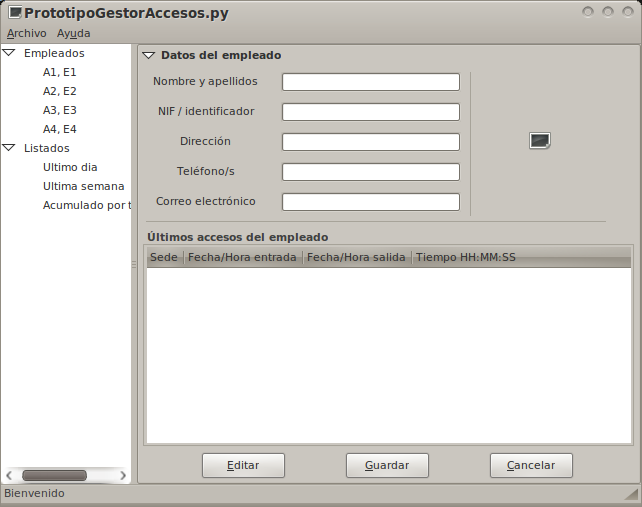
\includegraphics[width=8cm]{PrototipoGestorAccesos.png}
        \caption{Interfaz de gestión de accesos (prototipo)}
	\label{fig:gestion_accesos}
\end{figure}


\section{Base de datos biométricos}
Tras una toma de estadísticas y la consideración de cuál es el mejor método de almacenamiento de datos para las huellas faciales, se procederá a la creación de la base de datos biométricos.

\section{Interfaz de Reconocimiento}
Actualmente se encuentra en estado beta. Faltan por pulir detalles en cuanto a diálogos de configuración, tratamiento de errores y diálogos de "Acerca de".

\begin{figure}[h!]
        \centering
        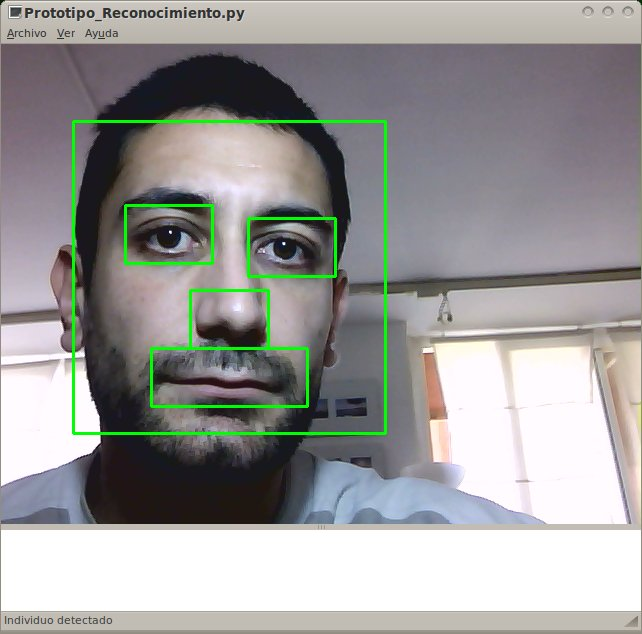
\includegraphics[width=8cm]{PrototipoReconocimiento.jpg}
        \caption{Interfaz de Reconocimiento (prototipo)}
	\label{fig:reconocimiento}
\end{figure}

\section{Interfaz de Captura}
Todavía no disponible. En cuanto se haya determinado el mejor método para almacenar los datos biométricos, se iniciará.


\chapter{Licencia de la memoria}
\label{app:docLicense}
% This file was converted from HTML to LaTeX with
% Tomasz Wegrzanowski's <maniek@beer.com> gnuhtml2latex program
% Version : 0.1
\section*{Código Legal de Creative Commons}
      
        \subsection*{Reconocimiento-CompartirIgual 3.0 España}
      	\begin{center}
		
\includegraphics{imagenes/cc-by-sa.png}
	\end{center}

         CREATIVE COMMONS CORPORATION NO ES UN DESPACHO DE ABOGADOS Y NO PROPORCIONA SERVICIOS JURÍDICOS. LA DISTRIBUCIÓN DE ESTA LICENCIA NO CREA UNA RELACIÓN ABOGADO-CLIENTE. CREATIVE COMMONS PROPORCIONA ESTA INFORMACIÓN TAL CUAL (ON AN 'AS-IS' BASIS). CREATIVE COMMONS NO OFRECE GARANTÍA ALGUNA RESPECTO DE LA INFORMACIÓN PROPORCIONADA, NI ASUME RESPONSABILIDAD ALGUNA POR DAÑOS PRODUCIDOS A CONSECUENCIA DE SU USO.

        \subsubsection*{\emph{Licencia}}

        \par LA OBRA O LA PRESTACIÓN (SEGÚN SE DEFINEN MÁS ADELANTE) SE PROPORCIONA BAJO LOS TÉRMINOS DE ESTA LICENCIA PÚBLICA DE CREATIVE COMMONS (\textbf{\emph{CCPL}} O \textbf{\emph{LICENCIA}}). LA OBRA O LA PRESTACIÓN  SE ENCUENTRA PROTEGIDA POR LA LEY ESPAÑOLA DE PROPIEDAD INTELECTUAL Y/O CUALESQUIERA OTRAS NORMAS QUE RESULTEN DE APLICACIÓN. QUEDA PROHIBIDO CUALQUIER USO DE LA OBRA O PRESTACIÓN DIFERENTE A LO AUTORIZADO BAJO ESTA LICENCIA O LO DISPUESTO EN LA LEY DE PROPIEDAD INTELECTUAL.\\

        \par MEDIANTE EL EJERCICIO DE CUALQUIER DERECHO SOBRE LA OBRA O LA PRESTACIÓN, USTED ACEPTA Y CONSIENTE LAS LIMITACIONES Y OBLIGACIONES DE ESTA LICENCIA, SIN PERJUICIO DE LA NECESIDAD DE CONSENTIMIENTO EXPRESO EN CASO DE VIOLACIÓN PREVIA DE LOS TÉRMINOS DE LA MISMA. EL LICENCIADOR LE CONCEDE LOS DERECHOS CONTENIDOS EN ESTA LICENCIA, SIEMPRE QUE USTED ACEPTE LOS PRESENTES TÉRMINOS Y CONDICIONES. \\

        \par \textbf{1. Definiciones}

        \begin{enumerate}
          \item La \textbf{\emph{obra}} es la creación literaria, artística o científica ofrecida bajo los términos de esta licencia.

          \item En esta licencia se considera  una \textbf{\emph{prestación}} cualquier interpretación, ejecución, fonograma, grabación audiovisual, emisión o transmisión, mera fotografía u otros objetos protegidos por la legislación de propiedad intelectual vigente aplicable.

          \item La aplicación de esta licencia a una \textbf{\emph{colección}} (definida más adelante) afectará únicamente a su estructura en cuanto forma de expresión de la selección o disposición de sus contenidos, no siendo extensiva a éstos. En este caso la colección tendrá la consideración de obra a efectos de esta licencia.

          \item El \textbf{\emph{titular originario}} es: 
        \begin{enumerate}
          \item En el caso de una obra literaria, artística o científica, la persona natural o grupo de personas que creó la obra.
          \item En el caso de una obra colectiva, la persona que la edite y divulgue bajo su nombre, salvo pacto contrario.
          \item En el caso de una interpretación o ejecución, el actor, cantante, músico, o cualquier otra persona que represente, cante, lea, recite, interprete o ejecute en cualquier forma una obra. 
          \item En el caso de un fonograma, el productor fonográfico, es decir, la persona natural o jurídica bajo cuya iniciativa y responsabilidad se realiza por primera vez una fijación exclusivamente sonora de la ejecución de una obra o de otros sonidos.
          \item En el caso de una grabación audiovisual, el productor de la grabación, es decir, la persona natural o jurídica que tenga la iniciativa y asuma la responsabilidad de las fijaciones de un plano o secuencia de imágenes, con o sin sonido.
          \item En el caso de una emisión o una transmisión, la entidad de radiodifusión.
          \item En el caso de una mera fotografía, aquella persona que la haya realizado.
          \item En el caso de otros objetos protegidos por la legislación de propiedad intelectual vigente, la persona que ésta señale.
\end{enumerate}


          \item Se considerarán \textbf{\emph{obras derivadas}} aquellas obras creadas a partir de la licenciada, como por ejemplo: las traducciones y adaptaciones; las revisiones, actualizaciones y anotaciones; los compendios, resúmenes y extractos; los arreglos musicales y, en general, cualesquiera transformaciones de una obra literaria, artística o científica. Para evitar la duda, si la obra consiste en una composición musical o grabación de sonidos, la sincronización temporal de la obra con una imagen en movimiento (\emph{synching}) será considerada como una obra derivada a efectos de esta licencia.

          \item Tendrán la consideración de \textbf{\emph{colecciones}} la recopilación de obras ajenas, de datos o de otros elementos independientes como las antologías y las bases de datos que por la selección o disposición de sus contenidos constituyan creaciones intelectuales. La mera incorporación de una obra en una colección no dará lugar a una derivada a efectos de esta licencia.

          \item El \textbf{\emph{licenciador}} es la persona o la entidad que ofrece la obra o prestación bajo los términos de esta licencia y le concede los derechos de explotación de la misma conforme a lo dispuesto en ella. 

          \item \textbf{\emph{Usted}} es la persona o la entidad que ejercita los derechos concedidos mediante esta licencia y que no ha violado previamente los términos de la misma con respecto a la obra o la prestación, o que ha recibido el permiso expreso del licenciador de ejercitar los derechos concedidos mediante esta licencia a pesar de una violación anterior.

          \item La \textbf{\emph{transformación}} de una obra comprende su traducción, adaptación y cualquier otra modificación en su forma de la que se derive una obra diferente. La creación resultante de la transformación de una obra tendrá la consideración de obra derivada. 

         \item Se entiende por \textbf{\emph{reproducción}} la fijación directa o indirecta, provisional o permanente, por cualquier medio y en cualquier forma, de toda la obra o la prestación o de parte de ella, que permita su comunicación o la obtención de copias. 

	\item Se entiende por \textbf{\emph{distribución}} la puesta a disposición del público del original o de las copias de la obra o la prestación, en un soporte tangible, mediante su venta, alquiler, préstamo o de cualquier otra forma. 

     \item Se entiende por \textbf{\emph{comunicación pública}} todo acto por el cual una pluralidad de personas, que no pertenezcan al ámbito doméstico de quien la lleva a cabo,  pueda tener acceso a la obra o la prestación sin previa distribución de ejemplares a cada una de ellas. Se considera comunicación pública la puesta a disposición del público de obras o prestaciones por procedimientos alámbricos o inalámbricos, de tal forma que cualquier persona pueda acceder a ellas desde el lugar y en el momento que elija.

     \item La \textbf{\emph{explotación}} de la obra o la prestación comprende la reproducción, la distribución, la comunicación pública y, en su caso, la transformación.

     \item Los \textbf{\emph{elementos de la licencia}} son las características principales de la licencia según la selección efectuada por el licenciador e indicadas en el título de esta licencia: Reconocimiento, CompartirIgual.
\item Una \textbf{\emph{licencia equivalente}} es: 
	\begin{enumerate}
	\item Una versión posterior de esta licencia de Creative Commons con los mismos elementos de licencia.
	\item La misma versión o una versión posterior de esta licencia de cualquier otra jurisdicción reconocida por Creative Commons con los mismos elementos de la licencia (ejemplo: Reconocimiento-CompartirIgual 3.0 Japón).
        \item La misma versión o una versión posterior de la licencia de Creative Commons no adaptada a ninguna jurisdicción (\emph{Unported}) con los mismos elementos de la licencia.	
	\item Una de las licencias compatibles que aparece en http://creativecommons.org/compatiblelicenses y que ha sido aprobada por Creative Commons como esencialmente equivalente a esta licencia porque, como mínimo:
		\begin{enumerate}
	\item Contiene términos con el mismo propósito, el mismo significado y el mismo efecto que los elementos de esta licencia.
	\item Permite explícitamente que las obras derivadas de obras sujetas a ella puedan ser distribuidas mediante esta licencia, la licencia de Creative Commons no adaptada a ninguna jurisdicción (\emph{Unported}) o una licencia de cualquier otra jurisdicción reconocida por Creative Commons, con sus mismos elementos de licencia.
	        \end{enumerate}
	
        \end{enumerate}

\end{enumerate}

        \par \textbf{2. Límites de los derechos.}\\
	 Nada en esta licencia pretende reducir o restringir cualesquiera límites legales de los derechos exclusivos del titular de los derechos de propiedad intelectual de acuerdo con la Ley de propiedad intelectual o cualesquiera otras leyes aplicables, ya sean derivados de usos legítimos, tales como la copia privada o la cita, u otras limitaciones como la resultante de la primera venta de ejemplares (agotamiento).\\

        \par \textbf{3. Concesión de licencia.} \\
	Conforme a los términos y a las condiciones de esta licencia, el licenciador concede, por el plazo de protección de los derechos de propiedad intelectual y a título gratuito, una licencia de ámbito mundial no exclusiva que incluye los derechos siguientes:

        \begin{enumerate}
          \item Derecho de reproducción, distribución y comunicación pública de la obra o la prestación.
          \item Derecho a incorporar la obra o la prestación en una o más colecciones.
          \item Derecho de reproducción, distribución y comunicación pública de la obra o la prestación lícitamente incorporada en una colección.
          \item Derecho de transformación de la obra para crear una obra derivada siempre y cuando se  incluya en ésta una indicación de la transformación o modificación efectuada.
          \item Derecho de reproducción, distribución y comunicación pública de obras derivadas creadas a partir de la obra licenciada.
          \item Derecho a extraer y reutilizar la obra o la prestación de una base de datos.
	 \item Para evitar cualquier duda, el titular originario:
        \begin{enumerate}
	\item Conserva el derecho a percibir las remuneraciones o compensaciones previstas por actos de explotación de la obra o prestación, calificadas por la ley como irrenunciables e inalienables y sujetas a gestión colectiva obligatoria.
	\item Renuncia  al derecho exclusivo a percibir, tanto individualmente como mediante una entidad de gestión colectiva de derechos, cualquier remuneración derivada de actos de explotación de la obra o prestación que usted realice.
        \end{enumerate}

        \end{enumerate}

        \par Estos derechos se pueden ejercitar en todos los medios y formatos, tangibles o intangibles, conocidos en el momento de la concesión de esta licencia. Los derechos mencionados incluyen el derecho a efectuar las modificaciones que sean precisas técnicamente para el ejercicio de los derechos en otros medios y formatos. Todos los derechos no concedidos expresamente por el licenciador quedan reservados, incluyendo, a título enunciativo pero no limitativo, los derechos morales irrenunciables reconocidos por la ley aplicable. En la medida en que el licenciador ostente derechos exclusivos previstos por la ley nacional vigente que implementa la directiva europea en materia de derecho sui generis sobre bases de datos, renuncia expresamente a dichos derechos exclusivos.\\


        \par \textbf{4. Restricciones.}\\
	 La concesión de derechos que supone esta licencia se encuentra sujeta y limitada a las restricciones siguientes:

        \begin{enumerate}
          \item Usted puede reproducir, distribuir o comunicar públicamente la obra o prestación solamente bajo los términos de esta licencia y debe incluir una copia de la misma, o su Identificador Uniforme de Recurso (URI). Usted no puede ofrecer o imponer ninguna condición sobre la obra o prestación que altere o restrinja los términos de esta licencia o el ejercicio de sus derechos por parte de los concesionarios de la misma. Usted no puede sublicenciar la obra o prestación. Usted debe mantener intactos todos los avisos que se refieran a esta licencia y a la ausencia de garantías. Usted no puede reproducir, distribuir o comunicar públicamente la obra o prestación  con medidas tecnológicas que controlen el acceso o el uso de una manera contraria a los términos de esta licencia. Esta sección 4.a también afecta a la obra o prestación incorporada en una colección, pero ello no implica que ésta en su conjunto quede automáticamente o deba quedar sujeta a los términos de la misma. En el caso que le sea requerido, previa comunicación del licenciador, si usted incorpora la obra en una colección y/o crea una obra derivada, deberá quitar cualquier crédito requerido en el apartado 4.c,  en la medida de lo posible.

	\item Usted puede distribuir o comunicar públicamente una obra derivada en el sentido de esta licencia solamente bajo los términos de la misma u otra licencia equivalente. Si usted utiliza esta misma licencia debe incluir una copia o bien su URI, con cada obra derivada que usted distribuya o comunique públicamente. Usted no puede ofrecer o imponer ningún término respecto a la obra derivada que altere o restrinja los términos de esta licencia o el ejercicio de sus derechos por parte de los concesionarios de la misma. Usted debe mantener intactos todos los avisos que se refieran a esta licencia y a la ausencia de garantías cuando distribuya o comunique públicamente la obra derivada. Usted no puede ofrecer o imponer ningún término respecto de las obras derivadas o sus transformaciones que alteren o restrinjan los términos de esta licencia o el ejercicio de sus derechos por parte de los concesionarios de la misma. Usted no puede reproducir, distribuir o comunicar públicamente la obra derivada con medidas tecnológicas que controlen el acceso o uso de la obra de una manera contraria a los términos de esta licencia. Si utiliza una licencia equivalente debe cumplir con los requisitos que ésta establezca cuando distribuya o comunique públicamente la obra derivada. Todas estas condiciones se aplican a una obra derivada en tanto que incorporada a una colección, pero no implica que ésta tenga que estar sujeta a los términos de esta licencia.

          \item Si usted reproduce, distribuye o comunica públicamente la obra o la prestación, una colección que la incorpore o cualquier obra derivada, debe mantener intactos todos los avisos sobre la propiedad intelectual e indicar, de manera razonable conforme al medio o a los medios que usted esté utilizando:
            \begin{enumerate}
		\item El nombre del autor original, o el seudónimo si es el caso, así como el del titular originario, si le es facilitado.
		\item El nombre de aquellas partes (por ejemplo: institución, publicación, revista) que el titular originario y/o el licenciador designen para ser reconocidos en el aviso legal, las condiciones de uso, o de cualquier otra manera razonable.
		\item El  título de la obra o la prestación si le es facilitado.
		\item El URI, si existe, que el licenciador especifique para ser vinculado a la obra o la prestación, a menos que tal URI no se refiera al aviso legal o a la información sobre la licencia de la obra o la prestación.
		\item En el caso de una obra derivada, un aviso que identifique la transformación de la obra en la obra derivada (p. ej., 'traducción castellana de la obra de Autor Original,' o 'guión basado en obra original de Autor Original').
\end{enumerate}
Este reconocimiento debe hacerse de manera razonable. En el caso de una obra derivada o incorporación en una colección estos créditos deberán aparecer como mínimo en el mismo lugar donde se hallen los correspondientes a otros autores o titulares y de forma comparable a los mismos. Para evitar la duda, los créditos requeridos en esta sección sólo serán utilizados a efectos de atribución de la obra o la prestación en la manera especificada anteriormente. Sin un permiso previo por escrito, usted no puede afirmar ni dar a entender implícitamente ni explícitamente ninguna conexión, patrocinio o aprobación por parte del titular originario, el licenciador y/o las partes reconocidas hacia usted o hacia el uso que hace de la obra o la prestación.

          \item Para evitar cualquier duda, debe hacerse notar que las restricciones anteriores (párrafos 4.a, 4.b y 4.c) no son de aplicación a aquellas partes de la obra o la prestación objeto de esta licencia que únicamente puedan ser protegidas mediante el derecho sui generis sobre bases de datos recogido por la ley nacional vigente implementando la directiva europea de bases de datos

         
 \end{enumerate}

        \par \textbf{5. Exoneración de responsabilidad} \\

        \par A MENOS QUE SE ACUERDE MUTUAMENTE ENTRE LAS PARTES, EL LICENCIADOR OFRECE LA OBRA O LA PRESTACIÓN TAL CUAL (ON AN 'AS-IS' BASIS) Y NO CONFIERE NINGUNA GARANTÍA DE CUALQUIER TIPO RESPECTO DE LA OBRA O LA PRESTACIÓN O DE LA PRESENCIA O AUSENCIA DE ERRORES QUE PUEDAN O NO SER DESCUBIERTOS. ALGUNAS JURISDICCIONES NO PERMITEN LA EXCLUSIÓN DE TALES GARANTÍAS, POR LO QUE TAL EXCLUSIÓN PUEDE NO SER DE APLICACIÓN A USTED. \\

        \par \textbf{6. Limitación de responsabilidad.} SALVO QUE LO DISPONGA EXPRESA E IMPERATIVAMENTE LA LEY APLICABLE, EN NINGÚN CASO EL LICENCIADOR SERÁ RESPONSABLE ANTE USTED POR CUALESQUIERA DAÑOS RESULTANTES, GENERALES O ESPECIALES (INCLUIDO EL DAÑO EMERGENTE Y EL LUCRO CESANTE), FORTUITOS O CAUSALES, DIRECTOS O INDIRECTOS, PRODUCIDOS EN CONEXIÓN CON ESTA LICENCIA O EL USO DE LA OBRA O LA PRESTACIÓN, INCLUSO SI EL LICENCIADOR HUBIERA SIDO INFORMADO DE LA POSIBILIDAD DE TALES DAÑOS. \\


        \par \textbf{7. Finalización de la licencia} 

        \begin{enumerate}
          \item Esta licencia y la concesión de los derechos que contiene terminarán automáticamente en caso de cualquier incumplimiento de los términos de la misma. Las personas o entidades que hayan recibido de usted obras derivadas o colecciones bajo esta licencia, sin embargo, no verán sus licencias finalizadas, siempre que tales personas o entidades se mantengan en el cumplimiento íntegro de esta licencia. Las secciones 1, 2, 5, 6, 7 y 8 permanecerán vigentes pese a cualquier finalización de esta licencia.

          \item Conforme a las condiciones y términos anteriores, la concesión de derechos de esta licencia es vigente por todo el plazo de protección de los derechos de propiedad intelectual según la ley aplicable. A pesar de lo anterior, el licenciador se reserva el derecho a divulgar o publicar la obra o la prestación en condiciones distintas a las presentes, o de retirar la obra o la prestación en cualquier momento. No obstante, ello no supondrá dar por concluida esta licencia (o cualquier otra licencia que haya sido concedida, o sea necesario ser concedida, bajo los términos de esta licencia), que continuará vigente y con efectos completos a no ser que haya finalizado conforme a lo establecido anteriormente, sin perjuicio del derecho moral de arrepentimiento en los términos reconocidos por la ley de propiedad intelectual aplicable.
        \end{enumerate}

        \par \textbf{8. Miscelánea}

        \begin{enumerate}
          \item Cada vez que usted realice cualquier tipo de explotación de la obra o la prestación, o de una colección que la incorpore, el licenciador ofrece a los terceros y sucesivos licenciatarios la concesión de derechos sobre la obra o la prestación en las mismas condiciones y términos que la licencia concedida a usted.

          \item Cada vez que usted realice cualquier tipo de explotación de una obra derivada, el licenciador  ofrece a los terceros y sucesivos licenciatarios la concesión de derechos sobre la obra objeto de esta licencia en las mismas condiciones y términos que la licencia concedida a usted. 

          \item Si alguna disposición de esta licencia resulta inválida o inaplicable según la Ley vigente, ello no afectará la validez o aplicabilidad del resto de los términos de esta licencia y, sin ninguna acción adicional por cualquiera las partes de este acuerdo, tal disposición se entenderá reformada en lo estrictamente necesario para hacer que tal disposición sea válida y ejecutiva.

          \item No se entenderá que existe renuncia respecto de algún término o disposición de esta licencia, ni que se consiente violación alguna de la misma, a menos que tal renuncia o consentimiento figure por escrito y lleve la firma de la parte que renuncie o consienta. 

          \item Esta licencia constituye el acuerdo pleno entre las partes con respecto a la obra o la prestación objeto de la licencia. No caben interpretaciones, acuerdos o condiciones  con respecto a la obra o la prestación que no se encuentren expresamente especificados en la presente licencia. El licenciador no estará obligado por ninguna disposición complementaria que pueda aparecer en cualquier comunicación que le haga llegar usted. Esta licencia no se puede modificar sin el mutuo acuerdo por escrito entre el licenciador y usted.
        \end{enumerate}
        
          \subsubsection*{Aviso de Creative Commons}

          \par Creative Commons no es parte de esta licencia, y no ofrece ninguna garantía en relación con la obra o la prestación. Creative Commons no será responsable frente a usted o a cualquier parte, por cualesquiera daños resultantes, incluyendo, pero no limitado, daños generales o especiales (incluido el daño emergente y el lucro cesante), fortuitos o causales, en conexión con esta licencia. A pesar de las dos (2) oraciones anteriores, si Creative Commons se ha identificado expresamente como el licenciador, tendrá todos los derechos y obligaciones del licenciador. \\

          \par Salvo para el propósito limitado de indicar al público que la obra o la prestación está licenciada bajo la CCPL, ninguna parte utilizará la marca registrada 'Creative Commons' o cualquier marca registrada o insignia relacionada con 'Creative Commons' sin su consentimiento por escrito. Cualquier uso permitido se hará de conformidad con las pautas vigentes en cada momento sobre el uso de la marca registrada por 'Creative Commons', en tanto que sean publicadas su sitio web (website) o sean proporcionadas a petición previa. Para evitar cualquier duda, estas restricciones en el uso de la marca no forman parte de esta licencia. \\

          \par Puede contactar con Creative Commons en: http://creativecommons.org/.
        
      
    



\chapter{Licencia del código}
%\title{GNU GENERAL PUBLIC LICENSE}
%\date{Version 3, 29 June 2007}

%\begin{document}
%\maketitle

\begin{center}
{\parindent 0in

Copyright \copyright\  2007 Free Software Foundation, Inc. \texttt{http://fsf.org/}

\bigskip
Everyone is permitted to copy and distribute verbatim copies of this

license document, but changing it is not allowed.}

\end{center}

%\renewcommand{\abstractname}{Preamble}
The GNU General Public License is a free, copyleft license for
software and other kinds of works.

The licenses for most software and other practical works are designed
to take away your freedom to share and change the works.  By contrast,
the GNU General Public License is intended to guarantee your freedom to
share and change all versions of a program--to make sure it remains free
software for all its users.  We, the Free Software Foundation, use the
GNU General Public License for most of our software; it applies also to
any other work released this way by its authors.  You can apply it to
your programs, too.

When we speak of free software, we are referring to freedom, not
price.  Our General Public Licenses are designed to make sure that you
have the freedom to distribute copies of free software (and charge for
them if you wish), that you receive source code or can get it if you
want it, that you can change the software or use pieces of it in new
free programs, and that you know you can do these things.

To protect your rights, we need to prevent others from denying you
these rights or asking you to surrender the rights.  Therefore, you have
certain responsibilities if you distribute copies of the software, or if
you modify it: responsibilities to respect the freedom of others.

For example, if you distribute copies of such a program, whether
gratis or for a fee, you must pass on to the recipients the same
freedoms that you received.  You must make sure that they, too, receive
or can get the source code.  And you must show them these terms so they
know their rights.

Developers that use the GNU GPL protect your rights with two steps:
(1) assert copyright on the software, and (2) offer you this License
giving you legal permission to copy, distribute and/or modify it.

For the developers' and authors' protection, the GPL clearly explains
that there is no warranty for this free software.  For both users' and
authors' sake, the GPL requires that modified versions be marked as
changed, so that their problems will not be attributed erroneously to
authors of previous versions.

Some devices are designed to deny users access to install or run
modified versions of the software inside them, although the manufacturer
can do so.  This is fundamentally incompatible with the aim of
protecting users' freedom to change the software.  The systematic
pattern of such abuse occurs in the area of products for individuals to
use, which is precisely where it is most unacceptable.  Therefore, we
have designed this version of the GPL to prohibit the practice for those
products.  If such problems arise substantially in other domains, we
stand ready to extend this provision to those domains in future versions
of the GPL, as needed to protect the freedom of users.

Finally, every program is threatened constantly by software patents.
States should not allow patents to restrict development and use of
software on general-purpose computers, but in those that do, we wish to
avoid the special danger that patents applied to a free program could
make it effectively proprietary.  To prevent this, the GPL assures that
patents cannot be used to render the program non-free.

The precise terms and conditions for copying, distribution and
modification follow.

\begin{center}
{\Large \sc Terms and Conditions}
\end{center}


\begin{enumerate}

\addtocounter{enumi}{-1}

\item Definitions.

``This License'' refers to version 3 of the GNU General Public License.

``Copyright'' also means copyright-like laws that apply to other kinds of
works, such as semiconductor masks.

``The Program'' refers to any copyrightable work licensed under this
License.  Each licensee is addressed as ``you''.  ``Licensees'' and
``recipients'' may be individuals or organizations.

To ``modify'' a work means to copy from or adapt all or part of the work
in a fashion requiring copyright permission, other than the making of an
exact copy.  The resulting work is called a ``modified version'' of the
earlier work or a work ``based on'' the earlier work.

A ``covered work'' means either the unmodified Program or a work based
on the Program.

To ``propagate'' a work means to do anything with it that, without
permission, would make you directly or secondarily liable for
infringement under applicable copyright law, except executing it on a
computer or modifying a private copy.  Propagation includes copying,
distribution (with or without modification), making available to the
public, and in some countries other activities as well.

To ``convey'' a work means any kind of propagation that enables other
parties to make or receive copies.  Mere interaction with a user through
a computer network, with no transfer of a copy, is not conveying.

An interactive user interface displays ``Appropriate Legal Notices''
to the extent that it includes a convenient and prominently visible
feature that (1) displays an appropriate copyright notice, and (2)
tells the user that there is no warranty for the work (except to the
extent that warranties are provided), that licensees may convey the
work under this License, and how to view a copy of this License.  If
the interface presents a list of user commands or options, such as a
menu, a prominent item in the list meets this criterion.

\item Source Code.

The ``source code'' for a work means the preferred form of the work
for making modifications to it.  ``Object code'' means any non-source
form of a work.

A ``Standard Interface'' means an interface that either is an official
standard defined by a recognized standards body, or, in the case of
interfaces specified for a particular programming language, one that
is widely used among developers working in that language.

The ``System Libraries'' of an executable work include anything, other
than the work as a whole, that (a) is included in the normal form of
packaging a Major Component, but which is not part of that Major
Component, and (b) serves only to enable use of the work with that
Major Component, or to implement a Standard Interface for which an
implementation is available to the public in source code form.  A
``Major Component'', in this context, means a major essential component
(kernel, window system, and so on) of the specific operating system
(if any) on which the executable work runs, or a compiler used to
produce the work, or an object code interpreter used to run it.

The ``Corresponding Source'' for a work in object code form means all
the source code needed to generate, install, and (for an executable
work) run the object code and to modify the work, including scripts to
control those activities.  However, it does not include the work's
System Libraries, or general-purpose tools or generally available free
programs which are used unmodified in performing those activities but
which are not part of the work.  For example, Corresponding Source
includes interface definition files associated with source files for
the work, and the source code for shared libraries and dynamically
linked subprograms that the work is specifically designed to require,
such as by intimate data communication or control flow between those
subprograms and other parts of the work.

The Corresponding Source need not include anything that users
can regenerate automatically from other parts of the Corresponding
Source.

The Corresponding Source for a work in source code form is that
same work.

\item Basic Permissions.

All rights granted under this License are granted for the term of
copyright on the Program, and are irrevocable provided the stated
conditions are met.  This License explicitly affirms your unlimited
permission to run the unmodified Program.  The output from running a
covered work is covered by this License only if the output, given its
content, constitutes a covered work.  This License acknowledges your
rights of fair use or other equivalent, as provided by copyright law.

You may make, run and propagate covered works that you do not
convey, without conditions so long as your license otherwise remains
in force.  You may convey covered works to others for the sole purpose
of having them make modifications exclusively for you, or provide you
with facilities for running those works, provided that you comply with
the terms of this License in conveying all material for which you do
not control copyright.  Those thus making or running the covered works
for you must do so exclusively on your behalf, under your direction
and control, on terms that prohibit them from making any copies of
your copyrighted material outside their relationship with you.

Conveying under any other circumstances is permitted solely under
the conditions stated below.  Sublicensing is not allowed; section 10
makes it unnecessary.

\item Protecting Users' Legal Rights From Anti-Circumvention Law.

No covered work shall be deemed part of an effective technological
measure under any applicable law fulfilling obligations under article
11 of the WIPO copyright treaty adopted on 20 December 1996, or
similar laws prohibiting or restricting circumvention of such
measures.

When you convey a covered work, you waive any legal power to forbid
circumvention of technological measures to the extent such circumvention
is effected by exercising rights under this License with respect to
the covered work, and you disclaim any intention to limit operation or
modification of the work as a means of enforcing, against the work's
users, your or third parties' legal rights to forbid circumvention of
technological measures.

\item Conveying Verbatim Copies.

You may convey verbatim copies of the Program's source code as you
receive it, in any medium, provided that you conspicuously and
appropriately publish on each copy an appropriate copyright notice;
keep intact all notices stating that this License and any
non-permissive terms added in accord with section 7 apply to the code;
keep intact all notices of the absence of any warranty; and give all
recipients a copy of this License along with the Program.

You may charge any price or no price for each copy that you convey,
and you may offer support or warranty protection for a fee.

\item Conveying Modified Source Versions.

You may convey a work based on the Program, or the modifications to
produce it from the Program, in the form of source code under the
terms of section 4, provided that you also meet all of these conditions:
  \begin{enumerate}
  \item The work must carry prominent notices stating that you modified
  it, and giving a relevant date.

  \item The work must carry prominent notices stating that it is
  released under this License and any conditions added under section
  7.  This requirement modifies the requirement in section 4 to
  ``keep intact all notices''.

  \item You must license the entire work, as a whole, under this
  License to anyone who comes into possession of a copy.  This
  License will therefore apply, along with any applicable section 7
  additional terms, to the whole of the work, and all its parts,
  regardless of how they are packaged.  This License gives no
  permission to license the work in any other way, but it does not
  invalidate such permission if you have separately received it.

  \item If the work has interactive user interfaces, each must display
  Appropriate Legal Notices; however, if the Program has interactive
  interfaces that do not display Appropriate Legal Notices, your
  work need not make them do so.
\end{enumerate}
A compilation of a covered work with other separate and independent
works, which are not by their nature extensions of the covered work,
and which are not combined with it such as to form a larger program,
in or on a volume of a storage or distribution medium, is called an
``aggregate'' if the compilation and its resulting copyright are not
used to limit the access or legal rights of the compilation's users
beyond what the individual works permit.  Inclusion of a covered work
in an aggregate does not cause this License to apply to the other
parts of the aggregate.

\item Conveying Non-Source Forms.

You may convey a covered work in object code form under the terms
of sections 4 and 5, provided that you also convey the
machine-readable Corresponding Source under the terms of this License,
in one of these ways:
  \begin{enumerate}
  \item Convey the object code in, or embodied in, a physical product
  (including a physical distribution medium), accompanied by the
  Corresponding Source fixed on a durable physical medium
  customarily used for software interchange.

  \item Convey the object code in, or embodied in, a physical product
  (including a physical distribution medium), accompanied by a
  written offer, valid for at least three years and valid for as
  long as you offer spare parts or customer support for that product
  model, to give anyone who possesses the object code either (1) a
  copy of the Corresponding Source for all the software in the
  product that is covered by this License, on a durable physical
  medium customarily used for software interchange, for a price no
  more than your reasonable cost of physically performing this
  conveying of source, or (2) access to copy the
  Corresponding Source from a network server at no charge.

  \item Convey individual copies of the object code with a copy of the
  written offer to provide the Corresponding Source.  This
  alternative is allowed only occasionally and noncommercially, and
  only if you received the object code with such an offer, in accord
  with subsection 6b.

  \item Convey the object code by offering access from a designated
  place (gratis or for a charge), and offer equivalent access to the
  Corresponding Source in the same way through the same place at no
  further charge.  You need not require recipients to copy the
  Corresponding Source along with the object code.  If the place to
  copy the object code is a network server, the Corresponding Source
  may be on a different server (operated by you or a third party)
  that supports equivalent copying facilities, provided you maintain
  clear directions next to the object code saying where to find the
  Corresponding Source.  Regardless of what server hosts the
  Corresponding Source, you remain obligated to ensure that it is
  available for as long as needed to satisfy these requirements.

  \item Convey the object code using peer-to-peer transmission, provided
  you inform other peers where the object code and Corresponding
  Source of the work are being offered to the general public at no
  charge under subsection 6d.
  \end{enumerate}

A separable portion of the object code, whose source code is excluded
from the Corresponding Source as a System Library, need not be
included in conveying the object code work.

A ``User Product'' is either (1) a ``consumer product'', which means any
tangible personal property which is normally used for personal, family,
or household purposes, or (2) anything designed or sold for incorporation
into a dwelling.  In determining whether a product is a consumer product,
doubtful cases shall be resolved in favor of coverage.  For a particular
product received by a particular user, ``normally used'' refers to a
typical or common use of that class of product, regardless of the status
of the particular user or of the way in which the particular user
actually uses, or expects or is expected to use, the product.  A product
is a consumer product regardless of whether the product has substantial
commercial, industrial or non-consumer uses, unless such uses represent
the only significant mode of use of the product.

``Installation Information'' for a User Product means any methods,
procedures, authorization keys, or other information required to install
and execute modified versions of a covered work in that User Product from
a modified version of its Corresponding Source.  The information must
suffice to ensure that the continued functioning of the modified object
code is in no case prevented or interfered with solely because
modification has been made.

If you convey an object code work under this section in, or with, or
specifically for use in, a User Product, and the conveying occurs as
part of a transaction in which the right of possession and use of the
User Product is transferred to the recipient in perpetuity or for a
fixed term (regardless of how the transaction is characterized), the
Corresponding Source conveyed under this section must be accompanied
by the Installation Information.  But this requirement does not apply
if neither you nor any third party retains the ability to install
modified object code on the User Product (for example, the work has
been installed in ROM).

The requirement to provide Installation Information does not include a
requirement to continue to provide support service, warranty, or updates
for a work that has been modified or installed by the recipient, or for
the User Product in which it has been modified or installed.  Access to a
network may be denied when the modification itself materially and
adversely affects the operation of the network or violates the rules and
protocols for communication across the network.

Corresponding Source conveyed, and Installation Information provided,
in accord with this section must be in a format that is publicly
documented (and with an implementation available to the public in
source code form), and must require no special password or key for
unpacking, reading or copying.

\item Additional Terms.

``Additional permissions'' are terms that supplement the terms of this
License by making exceptions from one or more of its conditions.
Additional permissions that are applicable to the entire Program shall
be treated as though they were included in this License, to the extent
that they are valid under applicable law.  If additional permissions
apply only to part of the Program, that part may be used separately
under those permissions, but the entire Program remains governed by
this License without regard to the additional permissions.

When you convey a copy of a covered work, you may at your option
remove any additional permissions from that copy, or from any part of
it.  (Additional permissions may be written to require their own
removal in certain cases when you modify the work.)  You may place
additional permissions on material, added by you to a covered work,
for which you have or can give appropriate copyright permission.

Notwithstanding any other provision of this License, for material you
add to a covered work, you may (if authorized by the copyright holders of
that material) supplement the terms of this License with terms:
  \begin{enumerate}
  \item Disclaiming warranty or limiting liability differently from the
  terms of sections 15 and 16 of this License; or

  \item Requiring preservation of specified reasonable legal notices or
  author attributions in that material or in the Appropriate Legal
  Notices displayed by works containing it; or

  \item Prohibiting misrepresentation of the origin of that material, or
  requiring that modified versions of such material be marked in
  reasonable ways as different from the original version; or

  \item Limiting the use for publicity purposes of names of licensors or
  authors of the material; or

  \item Declining to grant rights under trademark law for use of some
  trade names, trademarks, or service marks; or

  \item Requiring indemnification of licensors and authors of that
  material by anyone who conveys the material (or modified versions of
  it) with contractual assumptions of liability to the recipient, for
  any liability that these contractual assumptions directly impose on
  those licensors and authors.
  \end{enumerate}

All other non-permissive additional terms are considered ``further
restrictions'' within the meaning of section 10.  If the Program as you
received it, or any part of it, contains a notice stating that it is
governed by this License along with a term that is a further
restriction, you may remove that term.  If a license document contains
a further restriction but permits relicensing or conveying under this
License, you may add to a covered work material governed by the terms
of that license document, provided that the further restriction does
not survive such relicensing or conveying.

If you add terms to a covered work in accord with this section, you
must place, in the relevant source files, a statement of the
additional terms that apply to those files, or a notice indicating
where to find the applicable terms.

Additional terms, permissive or non-permissive, may be stated in the
form of a separately written license, or stated as exceptions;
the above requirements apply either way.

\item Termination.

You may not propagate or modify a covered work except as expressly
provided under this License.  Any attempt otherwise to propagate or
modify it is void, and will automatically terminate your rights under
this License (including any patent licenses granted under the third
paragraph of section 11).

However, if you cease all violation of this License, then your
license from a particular copyright holder is reinstated (a)
provisionally, unless and until the copyright holder explicitly and
finally terminates your license, and (b) permanently, if the copyright
holder fails to notify you of the violation by some reasonable means
prior to 60 days after the cessation.

Moreover, your license from a particular copyright holder is
reinstated permanently if the copyright holder notifies you of the
violation by some reasonable means, this is the first time you have
received notice of violation of this License (for any work) from that
copyright holder, and you cure the violation prior to 30 days after
your receipt of the notice.

Termination of your rights under this section does not terminate the
licenses of parties who have received copies or rights from you under
this License.  If your rights have been terminated and not permanently
reinstated, you do not qualify to receive new licenses for the same
material under section 10.

\item Acceptance Not Required for Having Copies.

You are not required to accept this License in order to receive or
run a copy of the Program.  Ancillary propagation of a covered work
occurring solely as a consequence of using peer-to-peer transmission
to receive a copy likewise does not require acceptance.  However,
nothing other than this License grants you permission to propagate or
modify any covered work.  These actions infringe copyright if you do
not accept this License.  Therefore, by modifying or propagating a
covered work, you indicate your acceptance of this License to do so.

\item Automatic Licensing of Downstream Recipients.

Each time you convey a covered work, the recipient automatically
receives a license from the original licensors, to run, modify and
propagate that work, subject to this License.  You are not responsible
for enforcing compliance by third parties with this License.

An ``entity transaction'' is a transaction transferring control of an
organization, or substantially all assets of one, or subdividing an
organization, or merging organizations.  If propagation of a covered
work results from an entity transaction, each party to that
transaction who receives a copy of the work also receives whatever
licenses to the work the party's predecessor in interest had or could
give under the previous paragraph, plus a right to possession of the
Corresponding Source of the work from the predecessor in interest, if
the predecessor has it or can get it with reasonable efforts.

You may not impose any further restrictions on the exercise of the
rights granted or affirmed under this License.  For example, you may
not impose a license fee, royalty, or other charge for exercise of
rights granted under this License, and you may not initiate litigation
(including a cross-claim or counterclaim in a lawsuit) alleging that
any patent claim is infringed by making, using, selling, offering for
sale, or importing the Program or any portion of it.

\item Patents.

A ``contributor'' is a copyright holder who authorizes use under this
License of the Program or a work on which the Program is based.  The
work thus licensed is called the contributor's ``contributor version''.

A contributor's ``essential patent claims'' are all patent claims
owned or controlled by the contributor, whether already acquired or
hereafter acquired, that would be infringed by some manner, permitted
by this License, of making, using, or selling its contributor version,
but do not include claims that would be infringed only as a
consequence of further modification of the contributor version.  For
purposes of this definition, ``control'' includes the right to grant
patent sublicenses in a manner consistent with the requirements of
this License.

Each contributor grants you a non-exclusive, worldwide, royalty-free
patent license under the contributor's essential patent claims, to
make, use, sell, offer for sale, import and otherwise run, modify and
propagate the contents of its contributor version.

In the following three paragraphs, a ``patent license'' is any express
agreement or commitment, however denominated, not to enforce a patent
(such as an express permission to practice a patent or covenant not to
sue for patent infringement).  To ``grant'' such a patent license to a
party means to make such an agreement or commitment not to enforce a
patent against the party.

If you convey a covered work, knowingly relying on a patent license,
and the Corresponding Source of the work is not available for anyone
to copy, free of charge and under the terms of this License, through a
publicly available network server or other readily accessible means,
then you must either (1) cause the Corresponding Source to be so
available, or (2) arrange to deprive yourself of the benefit of the
patent license for this particular work, or (3) arrange, in a manner
consistent with the requirements of this License, to extend the patent
license to downstream recipients.  ``Knowingly relying'' means you have
actual knowledge that, but for the patent license, your conveying the
covered work in a country, or your recipient's use of the covered work
in a country, would infringe one or more identifiable patents in that
country that you have reason to believe are valid.

If, pursuant to or in connection with a single transaction or
arrangement, you convey, or propagate by procuring conveyance of, a
covered work, and grant a patent license to some of the parties
receiving the covered work authorizing them to use, propagate, modify
or convey a specific copy of the covered work, then the patent license
you grant is automatically extended to all recipients of the covered
work and works based on it.

A patent license is ``discriminatory'' if it does not include within
the scope of its coverage, prohibits the exercise of, or is
conditioned on the non-exercise of one or more of the rights that are
specifically granted under this License.  You may not convey a covered
work if you are a party to an arrangement with a third party that is
in the business of distributing software, under which you make payment
to the third party based on the extent of your activity of conveying
the work, and under which the third party grants, to any of the
parties who would receive the covered work from you, a discriminatory
patent license (a) in connection with copies of the covered work
conveyed by you (or copies made from those copies), or (b) primarily
for and in connection with specific products or compilations that
contain the covered work, unless you entered into that arrangement,
or that patent license was granted, prior to 28 March 2007.

Nothing in this License shall be construed as excluding or limiting
any implied license or other defenses to infringement that may
otherwise be available to you under applicable patent law.

\item No Surrender of Others' Freedom.

If conditions are imposed on you (whether by court order, agreement or
otherwise) that contradict the conditions of this License, they do not
excuse you from the conditions of this License.  If you cannot convey a
covered work so as to satisfy simultaneously your obligations under this
License and any other pertinent obligations, then as a consequence you may
not convey it at all.  For example, if you agree to terms that obligate you
to collect a royalty for further conveying from those to whom you convey
the Program, the only way you could satisfy both those terms and this
License would be to refrain entirely from conveying the Program.

\item Use with the GNU Affero General Public License.

Notwithstanding any other provision of this License, you have
permission to link or combine any covered work with a work licensed
under version 3 of the GNU Affero General Public License into a single
combined work, and to convey the resulting work.  The terms of this
License will continue to apply to the part which is the covered work,
but the special requirements of the GNU Affero General Public License,
section 13, concerning interaction through a network will apply to the
combination as such.

\item Revised Versions of this License.

The Free Software Foundation may publish revised and/or new versions of
the GNU General Public License from time to time.  Such new versions will
be similar in spirit to the present version, but may differ in detail to
address new problems or concerns.

Each version is given a distinguishing version number.  If the
Program specifies that a certain numbered version of the GNU General
Public License ``or any later version'' applies to it, you have the
option of following the terms and conditions either of that numbered
version or of any later version published by the Free Software
Foundation.  If the Program does not specify a version number of the
GNU General Public License, you may choose any version ever published
by the Free Software Foundation.

If the Program specifies that a proxy can decide which future
versions of the GNU General Public License can be used, that proxy's
public statement of acceptance of a version permanently authorizes you
to choose that version for the Program.

Later license versions may give you additional or different
permissions.  However, no additional obligations are imposed on any
author or copyright holder as a result of your choosing to follow a
later version.

\item Disclaimer of Warranty.

\begin{sloppypar}
 THERE IS NO WARRANTY FOR THE PROGRAM, TO THE EXTENT PERMITTED BY
 APPLICABLE LAW.  EXCEPT WHEN OTHERWISE STATED IN WRITING THE
 COPYRIGHT HOLDERS AND/OR OTHER PARTIES PROVIDE THE PROGRAM ``AS IS''
 WITHOUT WARRANTY OF ANY KIND, EITHER EXPRESSED OR IMPLIED,
 INCLUDING, BUT NOT LIMITED TO, THE IMPLIED WARRANTIES OF
 MERCHANTABILITY AND FITNESS FOR A PARTICULAR PURPOSE.  THE ENTIRE
 RISK AS TO THE QUALITY AND PERFORMANCE OF THE PROGRAM IS WITH YOU.
 SHOULD THE PROGRAM PROVE DEFECTIVE, YOU ASSUME THE COST OF ALL
 NECESSARY SERVICING, REPAIR OR CORRECTION.
\end{sloppypar}

\item Limitation of Liability.

 IN NO EVENT UNLESS REQUIRED BY APPLICABLE LAW OR AGREED TO IN
 WRITING WILL ANY COPYRIGHT HOLDER, OR ANY OTHER PARTY WHO MODIFIES
 AND/OR CONVEYS THE PROGRAM AS PERMITTED ABOVE, BE LIABLE TO YOU FOR
 DAMAGES, INCLUDING ANY GENERAL, SPECIAL, INCIDENTAL OR CONSEQUENTIAL
 DAMAGES ARISING OUT OF THE USE OR INABILITY TO USE THE PROGRAM
 (INCLUDING BUT NOT LIMITED TO LOSS OF DATA OR DATA BEING RENDERED
 INACCURATE OR LOSSES SUSTAINED BY YOU OR THIRD PARTIES OR A FAILURE
 OF THE PROGRAM TO OPERATE WITH ANY OTHER PROGRAMS), EVEN IF SUCH
 HOLDER OR OTHER PARTY HAS BEEN ADVISED OF THE POSSIBILITY OF SUCH
 DAMAGES.

\item Interpretation of Sections 15 and 16.

If the disclaimer of warranty and limitation of liability provided
above cannot be given local legal effect according to their terms,
reviewing courts shall apply local law that most closely approximates
an absolute waiver of all civil liability in connection with the
Program, unless a warranty or assumption of liability accompanies a
copy of the Program in return for a fee.

\begin{center}
{\Large\sc End of Terms and Conditions}

\bigskip
How to Apply These Terms to Your New Programs
\end{center}

If you develop a new program, and you want it to be of the greatest
possible use to the public, the best way to achieve this is to make it
free software which everyone can redistribute and change under these terms.

To do so, attach the following notices to the program.  It is safest
to attach them to the start of each source file to most effectively
state the exclusion of warranty; and each file should have at least
the ``copyright'' line and a pointer to where the full notice is found.

{\footnotesize
\begin{verbatim}
<one line to give the program's name and a brief idea of what it does.>

Copyright (C) <textyear>  <name of author>

This program is free software: you can redistribute it and/or modify
it under the terms of the GNU General Public License as published by
the Free Software Foundation, either version 3 of the License, or
(at your option) any later version.

This program is distributed in the hope that it will be useful,
but WITHOUT ANY WARRANTY; without even the implied warranty of
MERCHANTABILITY or FITNESS FOR A PARTICULAR PURPOSE.  See the
GNU General Public License for more details.

You should have received a copy of the GNU General Public License
along with this program.  If not, see <http://www.gnu.org/licenses/>.
\end{verbatim}
}

Also add information on how to contact you by electronic and paper mail.

If the program does terminal interaction, make it output a short
notice like this when it starts in an interactive mode:

{\footnotesize
\begin{verbatim}
<program>  Copyright (C) <year>  <name of author>

This program comes with ABSOLUTELY NO WARRANTY; for details type `show w'.
This is free software, and you are welcome to redistribute it
under certain conditions; type `show c' for details.
\end{verbatim}
}

The hypothetical commands {\tt show w} and {\tt show c} should show
the appropriate
parts of the General Public License.  Of course, your program's commands
might be different; for a GUI interface, you would use an ``about box''.

You should also get your employer (if you work as a programmer) or
school, if any, to sign a ``copyright disclaimer'' for the program, if
necessary.  For more information on this, and how to apply and follow
the GNU GPL, see \texttt{http://www.gnu.org/licenses/}.

The GNU General Public License does not permit incorporating your
program into proprietary programs.  If your program is a subroutine
library, you may consider it more useful to permit linking proprietary
applications with the library.  If this is what you want to do, use
the GNU Lesser General Public License instead of this License.  But
first, please read \\
\texttt{http://www.gnu.org/philosophy/why-not-lgpl.html}.

\end{enumerate}



\end{document}
